%% ============================================================================
%%  ANALISI MATEMATICA — un corso rigoroso, spiegato passo per passo
%%  File principale.  Compilare con:   latexmk -lualatex main
%%
%%  Copyright (c) 2026 Biagio Raucci.
%%  Quest'opera è rilasciata con licenza Creative Commons
%%  Attribuzione - Condividi allo stesso modo 4.0 Internazionale (CC BY-SA 4.0).
%%  https://creativecommons.org/licenses/by-sa/4.0/
%% ============================================================================
\documentclass[11pt,a4paper,twoside,openright]{book}

%% --- stile del libro -------------------------------------------------------
\usepackage{stile/analisi}

%% --- florilegium: ornamenti floreali procedurali (LuaLaTeX, licenza MIT) ----
%  Il pacchetto vive in stile/florilegium/.  Lo carichiamo con l'opzione
%  `nomargin': il giardino viene disegnato soltanto nelle pagine di apertura
%  dei capitoli (si veda \aperturacapitolo in stile/teoremi.sty).
\directlua{
  % LuaTeX cerca i moduli Lua con kpathsea: aggiungiamo un cercatore per la
  % sottocartella del pacchetto, così `require("florilegium")' trova i file.
  table.insert(package.searchers, 2, function(name)
    local path = "stile/florilegium/" .. name .. ".lua"
    local f = io.open(path, "r")
    if f then f:close(); return loadfile(path) end
    return "\string\n\string\tno file '" .. path .. "'"
  end)}
\def\florilegiumseed{1972}            % seme fisso: il giardino non cambia tra le compilazioni
\usepackage[grown,nomargin,novisitors,density=0.8]{stile/florilegium/florilegium}
%  (l'avviso «You have requested package stile/florilegium/florilegium, but the
%   package provides florilegium» è innocuo: dipende solo dal percorso.)
\definecolor{ink}{HTML}{1F4E79}
\definecolor{accent}{HTML}{B4662F}

%% --- ambienti per teoremi, dimostrazioni, note, codice ---------------------
\usepackage{stile/teoremi}

%% --- metadati --------------------------------------------------------------
\title{Analisi Matematica}
\author{Biagio Raucci}
\date{\today}

\begin{document}

%% ===================== FRONTESPIZIO E PAGINE INIZIALI ======================
\frontmatter
%% ============================================================================
%%  Copertina
%%  Il giardino di florilegium cresce nel margine esterno; il frontespizio è
%%  disegnato in coordinate assolute di pagina (origine in basso a sinistra).
%% ============================================================================
\begin{titlepage}
\AddToShipoutPictureBG*{\AtPageLowerLeft{\margingardengrown}}%
\AddToShipoutPictureFG*{\AtPageLowerLeft{%
\begin{tikzpicture}[overlay]
  % barra verticale sul dorso
  \fill[blu] (0,0) rectangle (9mm,\paperheight);
  % filetti color rame
  \draw[rame, line width=0.8pt] (22mm,235mm) -- (140mm,235mm);
  \draw[rame, line width=0.8pt] (22mm,42mm) -- (140mm,42mm);
  % autore e titolo
  \node[anchor=north west, text width=118mm, align=left, inner sep=0pt]
    at (22mm,227mm) {%
      {\sffamily\color{grigio}\Large Biagio Raucci}\\[14mm]
      {\sffamily\bfseries\color{blu}\fontsize{44}{48}\selectfont Analisi\\[3mm] Matematica}\\[10mm]
      {\sffamily\color{grigio}\Large Un corso rigoroso,\\ spiegato passo per passo}\\[6mm]
      {\sffamily\color{grigio}\large Volume primo --- con figure, esercizi commentati\\ e codice Python}
    };
  % piede
  \node[anchor=south west, text width=118mm, align=left, inner sep=0pt]
    at (22mm,30mm) {%
      {\sffamily\color{grigio}\small Edizione aperta --- \the\year\\
       Testo rilasciato con licenza Creative Commons BY-SA 4.0}
    };
\end{tikzpicture}}}%
\null
\end{titlepage}

%% ============================================================================
%%  Colophon e licenza
%% ============================================================================
\clearpage
\thispagestyle{empty}
\null\vfill
\begin{flushleft}
\small
{\sffamily\bfseries\color{blu}Analisi Matematica} --- Un corso rigoroso, spiegato passo per passo.\\
Volume primo.\\[2mm]
Copyright \copyright{} \the\year{} Biagio Raucci.\\[4mm]

{\sffamily\bfseries\color{blu}Licenza.}
Quest'opera è rilasciata con licenza
\textbf{Creative Commons Attribuzione -- Condividi allo stesso modo 4.0 Internazionale}
(CC~BY-SA~4.0). Chiunque è libero di \emph{condividere} (riprodurre, distribuire,
comunicare al pubblico) e \emph{modificare} (remixare, trasformare il materiale e
basarsi su di esso per le proprie opere) per qualsiasi fine, anche commerciale, alle
seguenti condizioni: \emph{attribuzione} (è necessario riconoscere la paternità
dell'opera, fornire un link alla licenza e indicare se sono state effettuate delle
modifiche) e \emph{condivisione allo stesso modo} (se si trasforma il materiale, si deve
distribuire il proprio contributo con la stessa licenza dell'originale).
Il testo integrale della licenza è disponibile all'indirizzo\\
\url{https://creativecommons.org/licenses/by-sa/4.0/deed.it}\\[4mm]

{\sffamily\bfseries\color{blu}Sorgenti.}
Il libro è scritto in \LaTeX{} e i sorgenti --- testo, figure e codice Python ---
sono distribuiti insieme all'opera. La compilazione richiede \textsf{LuaLaTeX}:
\texttt{latexmk -lualatex main}.\\[4mm]

{\sffamily\bfseries\color{blu}Ringraziamenti e fonti.}
L'impostazione dei capitoli e la scelta degli argomenti seguono i classici corsi
universitari di Analisi Matematica Uno; in particolare i testi di P.~Marcellini e
C.~Sbordone, di E.~Giusti e di T.~Tao, e le dispense \emph{Analisi Uno} di E.~Paolini
(anch'esse rilasciate con licenza CC~BY-SA), che hanno ispirato la struttura di questo
progetto. Gli ornamenti floreali delle pagine di apertura sono generati dal pacchetto
\textsf{florilegium} di Kevin Raymond (licenza MIT), che disegna ogni petalo e ogni
foglia in Lua al momento della composizione: nessuna immagine è importata.\\[4mm]

{\sffamily\bfseries\color{blu}Software.}
Composto con \LaTeX{} (motore LuaTeX), font TeX Gyre Pagella e TeX Gyre Heros.
Figure realizzate con Ti\emph{k}Z, PGFPlots e Matplotlib.
\end{flushleft}
\vspace{10mm}

%% ============================================================================
%%  Dedica
%% ============================================================================
\cleardoublepage
\thispagestyle{empty}
\null\vspace*{0.22\textheight}
\begin{center}
  {\florilegiumornament[size=2.2em,ink=B4662F]{flower}}\\[10mm]
  {\large\itshape Ad Antonio e Umberto,}\\[8mm]
  \begin{minipage}{0.8\textwidth}
  \centering\itshape
  perché queste pagine, scritte pensando ai miei studenti,\\
  possano un giorno accompagnare anche voi:\\
  non come un elenco di risposte da ricordare,\\
  ma come un invito a cercare sempre,\\
  con pazienza e con coraggio, il perché delle cose.
  \end{minipage}
\end{center}
\vfill
\cleardoublepage

\cleardoublepage
\pdfbookmark[0]{Indice}{indice}
\tableofcontents
\cleardoublepage
%% ============================================================================
%%  Introduzione
%% ============================================================================
\chapter*{Introduzione}
\addcontentsline{toc}{chapter}{Introduzione}
\markboth{Introduzione}{Introduzione}
\AddToShipoutPictureBG*{\AtPageLowerLeft{\margingardengrown}}

\epigraph{La matematica è l'arte di dare lo stesso nome a cose diverse.}{Henri Poincaré}

\lettrine[lines=3, findent=2pt, nindent=0pt]{Q}{uesto libro} nasce da una convinzione
semplice: una dimostrazione non è una sequenza di formule da imparare a memoria, ma un
\emph{ragionamento}, e un ragionamento si può raccontare. Il programma è quello classico
dei corsi universitari di Analisi Matematica Uno --- i numeri reali, le successioni e le
serie, i limiti e la continuità, il calcolo differenziale e integrale --- e l'impostazione
è quella rigorosa e formale che la materia richiede. Ciò che cambia è il \emph{modo} in cui
le cose vengono dette: nessun passaggio viene lasciato al freddo formalismo, e per ogni
teorema il lettore viene accompagnato per mano nel piano della dimostrazione prima ancora
di leggerne i dettagli.

\section*{Come è organizzato ogni teorema}

Ogni risultato importante del libro è presentato secondo uno schema fisso, che il
lettore imparerà presto a riconoscere.

\begin{enumerate}[label=\textbf{\arabic*.}]
  \item \textbf{L'enunciato}, in una cornice azzurra, scritto nella forma più precisa
  possibile.
  \item \textbf{Lo schema dell'enunciato}, un riquadro in cui le \emph{ipotesi} e la
  \emph{tesi} sono esplicitate in modo schematico, separate l'una dall'altra. È un
  esercizio che consigliamo di fare da soli, coprendo il riquadro: saper dire con
  esattezza «che cosa si suppone» e «che cosa si vuole provare» è già metà del lavoro.
  \item \textbf{Il piano d'attacco}, in una cornice verde: \emph{come} affronteremo la
  dimostrazione, quale idea la guida, quali strumenti useremo e perché. È la parte che di
  solito manca nei libri di testo e che invece un buon insegnante racconta alla lavagna.
  \item \textbf{La dimostrazione} vera e propria, in cui ogni passaggio è giustificato con
  un rimando esplicito all'assioma, alla definizione o al risultato precedente che lo
  autorizza.
\end{enumerate}

Accanto a questo schema compaiono altri riquadri: le \textbf{definizioni} (color rame),
gli \textbf{esempi} e le \textbf{osservazioni} (grigio), le \textbf{note storiche} sui
matematici e sulle idee che incontreremo, le \textbf{avvertenze} sugli errori più comuni
e i riquadri di \textbf{codice Python}.

Alcuni teoremi hanno anche una \textbf{seconda dimostrazione}, preceduta da un piano
d'attacco intitolato «Un'altra via»: arrivare allo stesso risultato per una strada
diversa (l'estremo superiore al posto della bisezione, il valor medio al posto
dell'integrale) mostra quali ipotesi e quali idee sono davvero essenziali. Le
sottosezioni intitolate \textbf{Approfondimento} trattano argomenti che arricchiscono
il quadro senza essere indispensabili al seguito: l'assioma di Dedekind, il massimo e il
minimo limite, la quadratura della parabola di Archimede, le funzioni omogenee, i
prodotti infiniti. Molti di questi complementi, e numerose notizie storiche, seguono i
due volumi di Enrico Giusti \cite{giusti,giusti2}; in una prima lettura si possono
saltare.

Ogni capitolo, infine, si chiude con i
\textbf{punti fondamentali}: un riquadro azzurro che raccoglie le definizioni, i teoremi
e i metodi da ricordare, con i rimandi alle pagine in cui sono dimostrati, e un breve
paragrafo che collega il capitolo a quello successivo. È il punto da cui ripartire
quando si ripassa per l'esame.

\section*{Perché Python}

Un corso di Analisi è, per sua natura, un corso di \emph{idee}; ma le idee si capiscono
meglio quando si possono toccare. Abbiamo quindi inserito, dove pertinente, brevi
programmi in Python (con le librerie \texttt{numpy}, \texttt{matplotlib},
\texttt{sympy} e \texttt{fractions}) che permettono di verificare numericamente un
enunciato, di disegnare il grafico di una funzione, di esplorare che cosa succede quando
un'ipotesi viene a mancare, o di risolvere un esercizio. Tutte le figure generate al
calcolatore sono riproducibili con gli script distribuiti insieme ai sorgenti del libro,
nella cartella \texttt{python/}. Il codice non sostituisce mai la dimostrazione: la
affianca, come un laboratorio affianca un corso di fisica.

\section*{Il filo conduttore: i teoremi di esistenza}

Un corso di Analisi Matematica non è un elenco di formule, ma una catena di
argomentazioni logiche coerenti e conseguenti. Lo schema in \cref{fig:schema-teoremi}
riassume i collegamenti tra i principali teoremi (in genere \emph{di esistenza}) che
incontreremo in questo volume: tutto discende dall'\emph{assioma di completezza} dei
numeri reali, introdotto nel primo capitolo. Il lettore potrà tornare a questo schema
man mano che procede nello studio, e lo troverà utile anche nella preparazione
dell'esame.

\begin{figure}[p]
\centering
\begin{tikzpicture}[x=1cm, y=1cm,
  box/.style={draw=blu, fill=bluchiaro, rounded corners=2pt, text width=33mm,
    align=center, font=\scriptsize\sffamily, inner sep=3pt, minimum height=9mm},
  root/.style={box, fill=blu, text=white, font=\scriptsize\sffamily\bfseries},
  arr/.style={-{Latex[length=2mm]}, blu, thick},
  side/.style={-{Latex[length=2mm]}, rame, thick, dashed}]
  \def\dx{4.05}\def\dy{1.45}
  \node[root] (ass)     at (0,0)              {Assioma di completezza};
  \node[box]  (sup)     at (0,-\dy)           {Esistenza dell'estremo superiore};
  \node[box]  (mon)     at (0,-2*\dy)         {Esistenza del limite delle successioni monotòne};
  \node[box]  (bw)      at (-\dx,-3*\dy)      {Teorema di Bolzano--Weierstrass};
  \node[box]  (zeri)    at (\dx,-3*\dy)       {Teorema dell'esistenza degli zeri};
  \node[box]  (wei)     at (-\dx,-4*\dy)      {Teorema di Weierstrass};
  \node[box]  (cantor)  at (0,-4*\dy)         {Teorema di Cantor};
  \node[box]  (vi)      at (\dx,-4*\dy)       {Teorema dei valori intermedi};
  \node[box]  (rolle)   at (-\dx,-5*\dy)      {Teorema di Rolle};
  \node[box]  (integ)   at (0,-5*\dy)         {Integrabilità delle funzioni continue};
  \node[box]  (media)   at (\dx,-5*\dy)       {Teorema della media integrale};
  \node[box]  (lagr)    at (-\dx,-6*\dy)      {Teorema di Lagrange};
  \node[box]  (dernulla) at (0,-6*\dy)        {Funzioni con derivata nulla su un intervallo};
  \node[box]  (tfci)    at (\dx,-6*\dy)       {Teorema fondamentale del calcolo integrale};
  \node[box]  (cauchy)  at (-\dx,-7*\dy)      {Teorema di Cauchy};
  \node[box]  (prim)    at (0,-7*\dy)         {Caratterizzazione delle primitive};
  \node[box]  (ffci)    at (\dx,-7*\dy)       {Formula fondamentale del calcolo integrale};
  \node[box]  (hop)     at (-\dx,-8*\dy)      {Teorema di L'Hôpital};
  \node[box]  (tayint)  at (\dx,-8*\dy)       {Formula di Taylor con resto integrale};
  \node[box]  (peano)   at (-\dx,-9*\dy)      {Formula di Taylor con resto di Peano};
  \node[box]  (taylag)  at (\dx,-9*\dy)       {Formula di Taylor con resto di Lagrange};
  \draw[arr] (ass) -- (sup);
  \draw[arr] (sup) -- (mon);
  \draw[arr] (mon) -- (bw);
  \draw[arr] (mon) -- (zeri);
  \draw[arr] (bw) -- (wei);
  \draw[arr] (bw) -- (cantor);
  \draw[arr] (zeri) -- (vi);
  \draw[arr] (wei) -- (rolle);
  \draw[arr] (cantor) -- (integ);
  \draw[arr] (vi) -- (media);
  \draw[arr] (rolle) -- (lagr);
  \draw[arr] (integ) -- (dernulla);
  \draw[arr] (media) -- (tfci);
  \draw[arr] (lagr) -- (cauchy);
  \draw[side] (lagr) -- (dernulla);
  \draw[arr] (dernulla) -- (prim);
  \draw[arr] (tfci) -- (ffci);
  \draw[side] (prim) -- (ffci);
  \draw[arr] (cauchy) -- (hop);
  \draw[arr] (ffci) -- (tayint);
  \draw[arr] (hop) -- (peano);
  \draw[arr] (tayint) -- (taylag);
\end{tikzpicture}
\caption{Lo schema di collegamento dei principali teoremi di esistenza del corso. Le
frecce continue indicano «è usato nella dimostrazione di»; quelle tratteggiate un
contributo laterale. Oltre all'assioma di completezza, l'intero sistema degli assiomi dei
numeri reali è presupposto da tutta la teoria. Altre implicazioni importanti, non
riportate nello schema, sono quelle del teorema di Bolzano--Weierstrass, che implica il
criterio di convergenza di Cauchy, e del teorema dei valori intermedi, che implica la
continuità delle funzioni inverse e quindi la loro derivabilità.}
\label{fig:schema-teoremi}
\end{figure}

\section*{Avvertenze sulla notazione}

Scriviamo $\N=\{1,2,3,\dots\}$ per l'insieme dei numeri naturali (lo zero \emph{non} è
un numero naturale, in questo libro), $\Z$ per gli interi, $\Q$ per i razionali e
$\R$ per i reali. Il simbolo $\sen x$ indica il seno di $x$, secondo la consuetudine
italiana, e $\tg x$ la tangente. Il logaritmo senza indicazione della base, $\log x$, è
sempre il logaritmo naturale, in base $e$. Il simbolo $\blacksquare$ segna la fine di
una dimostrazione; i simboli $\implica$ e $\sse$ si leggono «implica» e «se e solo se»;
$\perogni$ si legge «per ogni» ed $\esiste$ «esiste».

\section*{Come usare questo libro}

Il consiglio più importante è di \emph{non} leggere le dimostrazioni passivamente.
Dopo l'enunciato, provate a scrivere da soli lo schema ipotesi/tesi; dopo il piano
d'attacco, provate a completare la dimostrazione prima di leggerla; dopo ogni esercizio
svolto, chiedetevi \emph{perché} si è scelta quella strada e non un'altra. È in queste
domande, più che nelle risposte, che si impara l'Analisi.


%% ============================ CAPITOLI =====================================
\mainmatter
%% ============================================================================
%%  CAPITOLO 1 — I numeri e le funzioni reali
%%  Fonte principale per argomenti e dimostrazioni: Marcellini–Sbordone, cap. 1.
%%  Il capitolo è suddiviso in file di paragrafo nella cartella cap01/.
%% ============================================================================
\aperturacapitolo{I numeri e le funzioni reali}{cap:numeri}

\epigraph{Dio ha creato i numeri interi; tutto il resto è opera dell'uomo.}{Leopold Kronecker}

\lettrine[lines=3, findent=2pt, nindent=0pt]{I}{l metodo} comunemente usato in
Matematica consiste nel precisare senza ambiguità i presupposti, da non cambiare durante
l'elaborazione della teoria, e nel dedurre da essi, in modo logico e coerente, il
maggior numero possibile di informazioni. I presupposti sono le \emph{regole del gioco}:
avrebbero potuto essere diverse, ma una volta iniziato il gioco non vengono più cambiate.
In Matematica tali presupposti si chiamano \emph{postulati} o \emph{assiomi}; da essi,
mediante dimostrazioni, si deducono i risultati, o \emph{teoremi}.

In questo capitolo fissiamo le regole del gioco dell'Analisi Matematica: gli assiomi dei
numeri reali. Vedremo che da una manciata di proprietà --- undici in tutto, e il lettore
le conosce quasi tutte fin dalle scuole elementari --- discende l'intero edificio della
teoria. Tra esse ce n'è una, l'\emph{assioma di completezza}, che il lettore
probabilmente non ha mai incontrato in forma esplicita, e che è il vero protagonista del
corso: è ciò che distingue i numeri reali dai numeri razionali, ed è ciò che rende
possibile parlare di limiti, di derivate e di integrali. Nella seconda parte del
capitolo richiameremo il linguaggio degli insiemi e delle funzioni, e passeremo in
rassegna le funzioni elementari (lineari, potenze, esponenziali, logaritmi,
trigonometriche) che useremo in tutto il libro.

\medskip
\noindent\textbf{In questo capitolo.}
\begin{itemize}
  \item Gli assiomi dei numeri reali e le loro prime conseguenze (\S\ref{sec:assiomi},
  \S\ref{sec:conseguenze}).
  \item Il linguaggio degli insiemi e delle relazioni (\S\ref{sec:insiemi}).
  \item I numeri naturali, interi, razionali; perché $\sqrt2$ non è razionale e perché
  $\Q$ non è completo (\S\ref{sec:nzq}).
  \item Approfondimento: l'assioma di Dedekind (\S\ref{subsec:assioma-dedekind}) e un
  modello dei numeri reali costruito a partire da $\Q$ (\S\ref{subsec:modello-reali}).
  \item Funzioni, grafici, funzioni iniettive, suriettive, invertibili, monotòne
  (\S\ref{sec:funzioni}, \S\ref{sec:invertibili}).
  \item Le funzioni elementari: lineari, valore assoluto, potenze, esponenziali,
  logaritmi, trigonometriche (\S\ref{sec:lineari}--\S\ref{sec:trigonometriche}).
  \item Il principio di induzione (\S\ref{sec:induzione}).
  \item Esercizi di riepilogo (\S\ref{sec:esercizi-cap1}).
  \item Punti fondamentali del capitolo (\S\ref{sec:sintesi-cap01}).
\end{itemize}

%% ----------------------------------------------------------------------------
%%  §1.1  Gli assiomi dei numeri reali
%% ----------------------------------------------------------------------------
\section{Gli assiomi dei numeri reali}
\label{sec:assiomi}

Il nostro punto di partenza è quello di \emph{assumere, come postulato, che esista il
sistema dei numeri reali}. Assumiamo cioè che esista un insieme, che chiamiamo insieme
dei numeri reali e che indichiamo con $\R$, i cui elementi si possono sommare e
moltiplicare e si possono confrontare tra loro, e che tali operazioni e tale confronto
obbediscano a un certo numero di regole. Sono le regole che il lettore ha sempre usato,
in modo naturale, da quando ha imparato a far di conto: per tutti è ovvio che $2+3$ sia
uguale a $3+2$, o che $2\cdot3=3\cdot2$. Esprimiamo questo fatto in generale, per due
numeri reali $a$ e $b$, dicendo che valgono le \emph{proprietà commutative} della
somma e del prodotto:
\begin{equation}\label{eq:commutativa}
  a+b=b+a, \qquad a\cdot b=b\cdot a .
\end{equation}
Il lettore conosce sicuramente (provi a scriverle da solo, prima di proseguire) anche
la proprietà associativa, sia rispetto alla somma sia rispetto al prodotto, e la
proprietà distributiva. Elenchiamo ora in modo completo le proprietà che assumiamo
valere \emph{per assioma}, dividendole in tre gruppi: le proprietà relative alle
operazioni, le proprietà relative all'ordinamento e l'assioma di completezza.

\begin{notastorica}[Che cosa sono i numeri reali?]
Per secoli i matematici hanno usato i numeri reali senza una definizione precisa: la
«retta dei numeri» era un'immagine geometrica sufficiente per Newton e per Eulero. Fu
solo nella seconda metà dell'Ottocento, con Richard Dedekind (1831--1916), Georg Cantor
(1845--1918) e Karl Weierstrass (1815--1897), che si sentì il bisogno di \emph{costruire}
$\R$ a partire dai numeri razionali, per dare un fondamento rigoroso al calcolo
infinitesimale. Dedekind, in \emph{Stetigkeit und irrationale Zahlen} (1872), racconta di
aver avuto l'idea delle sue «sezioni» il 24 novembre 1858, mentre preparava le lezioni
di calcolo al Politecnico di Zurigo, insoddisfatto di dover ricorrere all'intuizione
geometrica per dimostrare che una successione crescente e limitata ha un limite.
Nello stesso 1872 Cantor, e già nel 1869 il francese Charles Méray (1835--1911),
costruirono i reali per un'altra via, a partire dalle successioni di razionali che «si
stringono» (le successioni di Cauchy del \cref{sec:bw-cauchy}); Weierstrass ne esponeva
una sua nelle lezioni berlinesi. Il programma comune --- fondare l'intera Analisi sui
numeri naturali, attraverso i razionali --- fu chiamato da Felix Klein, nel 1895,
\emph{aritmetizzazione dell'analisi}. La frase di Kronecker in epigrafe ne riassume lo
spirito, anche se Kronecker stesso rifiutava le costruzioni di Dedekind e di Cantor,
che fanno uso di insiemi infiniti.
L'approccio di questo libro è diverso e più economico: non costruiamo i numeri reali,
ma \emph{postuliamo} che esistano con le proprietà elencate qui sotto. È l'approccio
\emph{assiomatico}, reso rigoroso da David Hilbert (1862--1943) nel 1900. I due approcci
sono equivalenti: si può dimostrare che esiste, a meno di «cambiare nome» agli elementi,
un solo sistema che soddisfa tutti gli assiomi che stiamo per enunciare (un modello
costruito con le sezioni di Dedekind è descritto nel \S\ref{subsec:modello-reali}).
\end{notastorica}

\subsection{Assiomi relativi alle operazioni}

Sono definite le operazioni di \emph{addizione} ($+$) e di \emph{moltiplicazione}
($\cdot$) tra coppie di numeri reali, con le seguenti proprietà ($a$, $b$, $c$ indicano
numeri reali generici).

\begin{assioma}[Proprietà delle operazioni]\label{ass:operazioni}
\leavevmode
\begin{enumerate}[label=\textup{(A\arabic*)}, ref=(A\arabic*), leftmargin=3em]
  \item\label{ass:associativa} \textbf{Proprietà associativa:}
    $(a+b)+c=a+(b+c)$ \ e \ $(a\cdot b)\cdot c=a\cdot(b\cdot c)$.
  \item\label{ass:commutativa} \textbf{Proprietà commutativa:}
    $a+b=b+a$ \ e \ $a\cdot b=b\cdot a$.
  \item\label{ass:distributiva} \textbf{Proprietà distributiva:}
    $a\cdot(b+c)=a\cdot b+a\cdot c$.
  \item\label{ass:neutri} \textbf{Esistenza degli elementi neutri:} esistono in $\R$ due
    numeri \emph{distinti}, indicati con $0$ e $1$, tali che $a+0=a$ e $a\cdot1=a$ per
    ogni $a\in\R$.
  \item\label{ass:opposto} \textbf{Esistenza degli opposti:} per ogni numero reale $a$
    esiste un numero reale, indicato con $-a$, tale che $a+(-a)=0$.
  \item\label{ass:inverso} \textbf{Esistenza degli inversi:} per ogni numero reale
    $a\neq0$ esiste un numero reale, indicato con $a^{-1}$, tale che $a\cdot a^{-1}=1$.
\end{enumerate}
\end{assioma}

\begin{osservazione}
Le proprietà (A1)--(A6) dicono, nel linguaggio dell'algebra, che $\R$ è un
\emph{campo}\index{campo}. Si noti che la sottrazione e la divisione non compaiono tra le
operazioni: esse sono \emph{definite} a partire dall'addizione e dalla moltiplicazione
ponendo
\[
  a-b \coloneqq a+(-b), \qquad \frac{a}{b}\coloneqq a\cdot b^{-1}\quad(b\neq0).
\]
Il simbolo $\coloneqq$ si legge «è definito uguale a». Si noti inoltre che nell'assioma
\ref{ass:inverso} si richiede $a\neq0$: vedremo nel \cref{sec:conseguenze} che questa
restrizione non è un capriccio, ma una necessità logica.
\end{osservazione}

\subsection{Assiomi relativi all'ordinamento}

È definita la relazione di \emph{minore o uguale} ($\le$) tra coppie di numeri reali,
con le seguenti proprietà.

\begin{assioma}[Proprietà dell'ordinamento]\label{ass:ordine}
\leavevmode
\begin{enumerate}[label=\textup{(O\arabic*)}, ref=(O\arabic*), leftmargin=3em]
  \item\label{ass:dicotomia} \textbf{Dicotomia:} per ogni coppia di numeri reali $a$, $b$ si
    ha $a\le b$ oppure $b\le a$.
  \item\label{ass:antisimmetrica} \textbf{Proprietà antisimmetrica:} se valgono
    contemporaneamente $a\le b$ e $b\le a$, allora $a=b$.
  \item\label{ass:ordine-somma} \textbf{Compatibilità con la somma:} se $a\le b$ allora
    $a+c\le b+c$ per ogni $c\in\R$.
  \item\label{ass:ordine-prodotto} \textbf{Compatibilità con il prodotto:} se $0\le a$ e
    $0\le b$ allora $0\le a+b$ e $0\le a\cdot b$.
\end{enumerate}
\end{assioma}

\begin{osservazione}
La proprietà di dicotomia \ref{ass:dicotomia}, applicata con $b=a$, dice in particolare
che $a\le a$ per ogni $a$ (\emph{proprietà riflessiva}). Tra gli assiomi non abbiamo
invece elencato la proprietà \emph{transitiva} («se $a\le b$ e $b\le c$ allora
$a\le c$»): la dimostreremo nel prossimo paragrafo come conseguenza degli altri assiomi.
Le relazioni $\ge$, $<$ e $>$ sono definite a partire da $\le$:
\begin{gather*}
  a\ge b \sse b\le a, \\
  a<b \sse (a\le b \text{ e } a\neq b), \qquad
  a>b \sse (a\ge b \text{ e } a\neq b).
\end{gather*}
Le relazioni $<$ e $>$ sono dette di \emph{minore stretto} e \emph{maggiore stretto}.
\end{osservazione}

\subsection{L'assioma di completezza}

\begin{assioma}[Completezza]\label{ass:completezza}\index{assioma di completezza}
Siano $A$ e $B$ due insiemi non vuoti di numeri reali con la proprietà che
\[
  a\le b \qquad\text{comunque si scelgano } a\in A \text{ e } b\in B.
\]
Allora esiste almeno un numero reale $c$ tale che
\[
  a\le c\le b \qquad\text{qualunque siano } a\in A \text{ e } b\in B.
\]
\end{assioma}

\begin{marginfigure}
\centering
\begin{tikzpicture}[scale=0.9]
  \draw[-Latex, grigio] (-0.3,0) -- (5.2,0);
  \foreach \x in {0.2,0.6,1.0,1.5,1.9,2.2} \fill[blu] (\x,0) circle (1.6pt);
  \foreach \x in {3.0,3.3,3.8,4.3,4.8} \fill[rame] (\x,0) circle (1.6pt);
  \draw[blu, thick, decorate, decoration={brace, amplitude=4pt, mirror}] (0.1,-0.25) -- (2.3,-0.25)
    node[midway, below=5pt, font=\scriptsize] {$A$};
  \draw[rame, thick, decorate, decoration={brace, amplitude=4pt, mirror}] (2.9,-0.25) -- (4.9,-0.25)
    node[midway, below=5pt, font=\scriptsize] {$B$};
  \draw[verde, thick] (2.6,-0.15) -- (2.6,0.15) node[above, font=\scriptsize] {$c$};
\end{tikzpicture}
\caption{L'assioma di completezza: se ogni elemento di $A$ precede ogni elemento di $B$,
esiste un «separatore» $c$.}
\label{fig:completezza}
\end{marginfigure}

A prima vista l'assioma di completezza può sembrare ovvio, e il lettore potrebbe essere
tentato di «dimostrarlo» così: «se tutti i numeri dell'insieme $A$ sono minori o uguali
di tutti i numeri dell'insieme $B$, allora esisterà certamente un numero $c$
intermedio tra $A$ e $B$; basterà infatti scegliere come $c$ il più grande elemento di
$A$, oppure il più piccolo elemento di $B$».

\begin{attenzione}[La frase precedente è sbagliata!]
Non tutti gli insiemi numerici hanno un più grande o un più piccolo elemento. Ad
esempio, l'insieme
\[
  B=\set{1,\ \tfrac12,\ \tfrac13,\ \tfrac14,\ \dots,\ \tfrac1n,\ \dots},
\]
rappresentato sulla retta nella \cref{fig:insieme-1-su-n}, ha il più grande elemento,
che è $1$, ma \emph{non} ha il più piccolo elemento. Potremmo essere tentati di dire
che lo zero è il più piccolo elemento di $B$; ma lo zero \emph{non è un elemento di
$B$}! Infatti $0\neq 1/n$ qualunque sia $n$, perché una frazione è nulla se e soltanto
se il suo numeratore è nullo. Gli elementi di $B$ si accumulano verso lo zero senza
mai raggiungerlo, e per ogni elemento $1/n$ di $B$ ce n'è uno più piccolo,
$1/(n+1)$.
\end{attenzione}

\begin{figure}[htb]
\centering
\begin{tikzpicture}[scale=1.0]
  \draw[-Latex, grigio] (-0.5,0) -- (11.3,0) node[below left, font=\scriptsize] {};
  \foreach \n in {1,...,60} {\fill[blu] ({10/\n},0) circle (1.3pt);}
  \draw[rosso, thick] (0,0) circle (2.2pt);
  \node[below, font=\scriptsize] at (0,-0.1) {$0$};
  \foreach \n/\lab in {1/1, 2/\tfrac12, 3/\tfrac13, 4/\tfrac14, 5/\tfrac15, 8/\tfrac18} {
    \draw[grigio] ({10/\n},0.08) -- ({10/\n},-0.08);
    \node[below, font=\scriptsize] at ({10/\n},-0.1) {$\lab$};}
\end{tikzpicture}
\caption{L'insieme $B=\{1/n : n\in\N\}$ ha massimo $1$ ma non ha minimo: i suoi
elementi si addensano verso $0$, che però (cerchietto rosso) non appartiene a $B$.}
\label{fig:insieme-1-su-n}
\end{figure}

L'assioma di completezza è, in effetti, un assioma molto più profondo di quanto possa
sembrare a prima vista. Come mostreremo nel \cref{sec:nzq}, soltanto tramite l'assioma di
completezza è possibile distinguere l'insieme dei numeri rappresentabili sotto forma di
frazione, i \emph{numeri razionali}, dall'insieme dei numeri reali: i razionali
soddisfano tutti gli assiomi (A1)--(A6) e (O1)--(O4), ma \emph{non} l'assioma di
completezza. In termini geometrici, l'assioma dice che la retta reale \emph{non ha
buchi}: se la tagliamo in due parti, una a sinistra e una a destra, il punto di taglio
è un numero reale.

\begin{idea}[Un'immagine fisica della completezza]
Si pensi a un'asta graduata e a un cursore che scorre su di essa. Se spingiamo il
cursore verso destra fin dove possiamo, con la regola «puoi avanzare finché resti a
sinistra di tutti i punti di $B$», il cursore si fermerà in una posizione precisa $c$:
non può «cadere in un buco» della retta. L'assioma di completezza garantisce che tale
posizione esista. Sui numeri razionali, invece, il cursore potrebbe trovarsi a dover
scegliere tra posizioni razionali sempre più vicine a un punto che razionale non è,
come $\sqrt2$, e non avrebbe dove fermarsi.
\end{idea}

\begin{python}[Verifica numerica delle proprietà di campo]
# Gli assiomi (A1)-(A6) si possono "toccare con mano" con numeri
# esatti: Fraction rappresenta i razionali senza arrotondamenti.
from fractions import Fraction as F

a, b, c = F(3, 4), F(-5, 6), F(7, 2)
print((a + b) + c == a + (b + c))      # (A1) associativa (somma)
print((a * b) * c == a * (b * c))      # (A1) associativa (prodotto)
print(a + b == b + a, a * b == b * a)  # (A2) commutativa
print(a * (b + c) == a * b + a * c)    # (A3) distributiva
print(a + 0 == a, a * 1 == a)          # (A4) elementi neutri
print(a + (-a) == 0)                   # (A5) opposto
print(a * (1 / a) == 1)                # (A6) inverso (a != 0)
\end{python}
\begin{risultato}
True
True
True True
True
True True
True
True
\end{risultato}

\begin{attenzione}[I numeri in virgola mobile non sono numeri reali]
Se nel codice precedente si sostituisce \texttt{Fraction} con i normali numeri
decimali (\texttt{float}), alcune uguaglianze possono fallire: ad esempio in Python
\texttt{0.1 + 0.2 == 0.3} restituisce \texttt{False}, e la proprietà associativa
\texttt{(0.1 + 0.2) + 0.3 == 0.1 + (0.2 + 0.3)} è anch'essa \texttt{False}. I
\texttt{float} sono un insieme \emph{finito} di numeri che approssima $\R$: ottimi per
calcolare, ma non obbediscono agli assiomi. Questa distinzione tra il modello matematico
(i numeri reali) e la sua rappresentazione al calcolatore è una delle prime cose che un
ingegnere deve avere chiara.
\end{attenzione}

%% ----------------------------------------------------------------------------
%%  §1.2  Alcune conseguenze degli assiomi dei numeri reali
%% ----------------------------------------------------------------------------
\section{Alcune conseguenze degli assiomi}
\label{sec:conseguenze}

Nel paragrafo precedente sono state elencate le proprietà dei numeri reali che vengono
assunte come assiomi. \emph{Tutte} le altre proprietà e tutti i teoremi esposti in
questo libro discendono dagli assiomi. Sono conseguenze degli assiomi anche quelle
proprietà elementari che fanno parte del «bagaglio matematico» di ogni studente, come il
fatto che \emph{un prodotto è nullo quando almeno uno dei due fattori è nullo}, oppure la
regola dei segni per il prodotto (che dagli studenti delle scuole elementari è talvolta
accettata come imposizione, perché incompresa) che schematicamente si enuncia:
\emph{meno per meno fa più}; oppure la norma, di frequente applicazione nel risolvere le
disequazioni, secondo cui \emph{moltiplicando entrambi i membri per una quantità
negativa il verso della disequazione cambia}.

Di seguito dimostriamo alcune di queste proprietà. Il lettore non si lasci ingannare
dalla loro apparente banalità: il valore di questo paragrafo sta nel \emph{metodo}. Ogni
passaggio deve essere giustificato da un assioma o da una proprietà già dimostrata, e
nient'altro; è lo stesso rigore che useremo per i teoremi più difficili del libro, e
conviene allenarlo su enunciati di cui si conosce già la risposta.

\subsection{Conseguenze degli assiomi delle operazioni}

\begin{proposizione}[Legge di semplificazione per la somma]\label{prop:semplificazione-somma}
Siano $a,b,c\in\R$. Se $a+b=a+c$, allora $b=c$.
\end{proposizione}

\begin{schema}
\Ipotesi{$a,b,c\in\R$ e $a+b=a+c$.}
\Tesi{$b=c$.}
\end{schema}

\begin{strategia}
Vogliamo «far sparire» $a$ dall'uguaglianza $a+b=a+c$. L'unico strumento che gli assiomi
ci offrono per cancellare un addendo è l'opposto: per \ref{ass:opposto} esiste $-a$ con
$a+(-a)=0$. L'idea è dunque di partire da $b$, scriverlo come $0+b$, sostituire $0$ con
$(-a)+a$ e poi, usando la proprietà associativa, far comparire il blocco $a+b$, che per
ipotesi vale $a+c$. A quel punto si ripercorre la strada a ritroso e si arriva a $c$.
\end{strategia}

\begin{dimostrazione}
Utilizziamo gli assiomi \ref{ass:neutri} e \ref{ass:opposto} (esistenza dello zero e
dell'opposto $-a$) e le proprietà commutativa \ref{ass:commutativa} e associativa
\ref{ass:associativa}:
\[
  b = 0+b = \bigl[a+(-a)\bigr]+b = \bigl[(-a)+a\bigr]+b = (-a)+(a+b).
\]
Essendo per ipotesi $a+b=a+c$, si ottiene
\begin{align*}
  b &= (-a)+(a+b) = (-a)+(a+c) = \bigl[(-a)+a\bigr]+c \\
    &= \bigl[a+(-a)\bigr]+c = 0+c = c+0 = c,
\end{align*}
che è la tesi.
\end{dimostrazione}

\begin{proposizione}[Legge di semplificazione per il prodotto]\label{prop:semplificazione-prodotto}
Siano $a,b,c\in\R$. Se $a\cdot b=a\cdot c$ e $a\neq0$, allora $b=c$.
\end{proposizione}

\begin{schema}
\Ipotesi{$a,b,c\in\R$, \ $a\cdot b=a\cdot c$ \ e \ $a\neq0$.}
\Tesi{$b=c$.}
\end{schema}

\begin{strategia}
Si procede esattamente come nella dimostrazione precedente, scambiando la somma con il
prodotto, lo zero con l'uno e l'opposto con l'inverso. L'unica accortezza è ricordare
che l'inverso $a^{-1}$ esiste \emph{purché} $a\neq0$, per \ref{ass:inverso}: ecco
perché l'ipotesi $a\neq0$ è indispensabile.
\end{strategia}

\begin{dimostrazione}
Poiché $a\neq0$, esiste l'inverso $a^{-1}$. Allora
\begin{align*}
  b &= b\cdot1 = 1\cdot b = (a\cdot a^{-1})\cdot b = (a^{-1}\cdot a)\cdot b \\
    &= a^{-1}\cdot(a\cdot b) = a^{-1}\cdot(a\cdot c) = (a^{-1}\cdot a)\cdot c \\
    &= (a\cdot a^{-1})\cdot c = 1\cdot c = c\cdot 1 = c. \qedhere
\end{align*}
\end{dimostrazione}

\begin{proposizione}[Legge di annullamento del prodotto]\label{prop:annullamento}
\index{legge di annullamento del prodotto}
Siano $a,b\in\R$. Il prodotto $a\cdot b$ è nullo se e soltanto se almeno uno dei due
fattori è nullo.
\end{proposizione}

\begin{schema}
\Ipotesi{$a,b\in\R$.}
\Tesi{$a\cdot b=0 \ \sse\ (a=0 \text{ oppure } b=0)$.}
\end{schema}

\begin{strategia}
L'enunciato è una doppia implicazione («se e soltanto se»): dobbiamo dimostrare due
cose distinte.
\begin{itemize}
  \item \textbf{Il «se»:} se $a=0$ oppure $b=0$ allora $a\cdot b=0$. Basta provare che
  $a\cdot0=0$ per ogni $a$. Sembra ovvio, ma non è un assioma! Lo zero è definito come
  elemento neutro della \emph{somma}, e nulla dice su come si comporta nel
  \emph{prodotto}. Il trucco è scrivere $0=1+0$ e usare la proprietà distributiva.
  \item \textbf{Il «soltanto se»:} se $a\cdot b=0$ allora $a=0$ oppure $b=0$. Se $a=0$
  non c'è nulla da dimostrare; se $a\neq0$ possiamo moltiplicare per $a^{-1}$ e usare la
  prima parte.
\end{itemize}
\end{strategia}

\begin{dimostrazione}
Proviamo preliminarmente l'implicazione con il «se», cioè che $a\cdot0=0$ per ogni
numero reale $a$. Ricordiamo che lo zero è, per l'assioma \ref{ass:neutri}, l'elemento
neutro rispetto alla somma, cioè $a+0=a$ per ogni $a$; e che $1$, elemento neutro
rispetto al prodotto, soddisfa $a\cdot1=a$. In base alla proprietà distributiva
\ref{ass:distributiva} abbiamo allora
\[
  a + a\cdot0 = a\cdot1 + a\cdot0 = a\cdot(1+0) = a\cdot1 = a = a+0,
\]
da cui, semplificando entrambi i membri in base alla
\cref{prop:semplificazione-somma}, otteniamo $a\cdot0=0$. Per la proprietà commutativa
vale anche $0\cdot b=0$.

Proviamo ora l'implicazione con il «soltanto se»: supponiamo $a\cdot b=0$. Se $a=0$
la tesi è raggiunta. Altrimenti, se $a\neq0$, esiste l'inverso $a^{-1}$ e si ha
\[
  b = b\cdot1 = b\cdot(a\cdot a^{-1}) = (b\cdot a)\cdot a^{-1}
    = (a\cdot b)\cdot a^{-1} = 0\cdot a^{-1} = 0 .
\]
Si noti che nell'ultimo passaggio abbiamo utilizzato quanto già provato nella prima
parte della dimostrazione.
\end{dimostrazione}

\begin{osservazione}[Perché non si può dividere per zero]
La \cref{prop:annullamento} spiega perché nell'ambito dei numeri reali non sia
possibile la divisione per zero, cioè perché nell'assioma \ref{ass:inverso} si richieda
$a\neq0$. Infatti, se fosse $a=0$, allora $a\cdot b=0\cdot b=0$ per ogni numero reale
$b$, e perciò \emph{non esiste} alcun numero reale $0^{-1}$ tale che $0\cdot0^{-1}=1$:
se esistesse, avremmo $1=0\cdot0^{-1}=0$, contro l'assioma \ref{ass:neutri} che
richiede $0\neq1$. La divisione per zero non è «vietata» da una regola arbitraria: è
\emph{impossibile} perché contraddittoria con gli assiomi.
\end{osservazione}

\begin{proposizione}[Unicità dell'opposto e dell'inverso]\label{prop:unicita}
\leavevmode
\begin{enumerate}
  \item L'opposto di un numero reale è unico.
  \item L'inverso di un numero reale non nullo è unico.
  \item Per ogni $a\in\R$ vale $-(-a)=a$.
\end{enumerate}
\end{proposizione}

\begin{schema}
\Ipotesi{$a\in\R$; per (ii) $a\neq0$.}
\Tesi{(i) se $a+x=0$ e $a+y=0$, allora $x=y$; \ (ii) se $a\cdot x=1$ e $a\cdot y=1$,
allora $x=y$; \ (iii) $-(-a)=a$.}
\end{schema}

\begin{strategia}
Per dimostrare che un oggetto è unico si procede sempre allo stesso modo: si suppone
che ce ne siano due, $x$ e $y$, con la stessa proprietà, e si dimostra che $x=y$. Qui
la proprietà è «$a+x=0$», e la legge di semplificazione fa il resto. Il punto (iii) è
un'applicazione dell'unicità: $-(-a)$ è \emph{per definizione} l'opposto di $-a$; ma
anche $a$ è un opposto di $-a$, perché $(-a)+a=0$; dunque i due coincidono.
\end{strategia}

\begin{dimostrazione}
(i) In base all'assioma \ref{ass:opposto}, per ogni numero reale $a$ esiste l'opposto
$-a$, tale che $a+(-a)=0$. Se supponiamo che risulti anche $a+b=0$ per qualche $b$,
allora $a+(-a)=a+b$ e, per la legge di semplificazione (\cref{prop:semplificazione-somma}),
$-a=b$: l'opposto è unico.

(ii) Stessa dimostrazione, con il prodotto al posto della somma e la
\cref{prop:semplificazione-prodotto} al posto della \cref{prop:semplificazione-somma}.

(iii) Il numero $-(-a)$ è, per definizione, l'opposto di $-a$. Ma essendo
$a+(-a)=(-a)+a=0$, risulta che anche $a$ è un opposto di $-a$; per l'unicità
dell'opposto provata in (i), $a=-(-a)$.
\end{dimostrazione}

\begin{proposizione}[Regola dei segni]\label{prop:segni}\index{regola dei segni}
Per ogni coppia di numeri reali $a$, $b$ risulta
\begin{enumerate}
  \item $(-a)\cdot b = -(a\cdot b)$;
  \item $(-a)\cdot(-b) = a\cdot b$.
\end{enumerate}
\end{proposizione}

\begin{schema}
\Ipotesi{$a,b\in\R$.}
\Tesi{(i) $(-a)\cdot b=-(a\cdot b)$; \quad (ii) $(-a)\cdot(-b)=a\cdot b$.}
\end{schema}

\begin{strategia}
Che cosa significa dimostrare che $(-a)\cdot b$ è uguale a $-(a\cdot b)$? Significa
dimostrare che $(-a)\cdot b$ è \emph{l'opposto} di $a\cdot b$, cioè che sommato ad
$a\cdot b$ dà zero; per l'unicità dell'opposto (\cref{prop:unicita}) ciò basta. E la
somma $(-a)\cdot b+a\cdot b$ si calcola con la proprietà distributiva, raccogliendo
$b$. Il punto (ii), il celebre «meno per meno fa più», si ottiene applicando due
volte il punto (i) e poi la regola $-(-x)=x$.
\end{strategia}

\begin{dimostrazione}
(i) Per la proprietà distributiva \ref{ass:distributiva} e per la
\cref{prop:annullamento} si ha
\[
  (-a)\cdot b + a\cdot b = \bigl[(-a)+a\bigr]\cdot b = 0\cdot b = 0,
\]
da cui $(-a)\cdot b$ è l'opposto di $a\cdot b$, cioè $(-a)\cdot b=-(a\cdot b)$.

(ii) Come conseguenza del punto (i), applicato due volte, e della proprietà commutativa
\ref{ass:commutativa}, abbiamo
\[
  (-a)\cdot(-b) = -\bigl[a\cdot(-b)\bigr] = -\bigl[(-b)\cdot a\bigr]
  = -\bigl[-(b\cdot a)\bigr] = -\bigl[-(a\cdot b)\bigr];
\]
la conclusione segue infine dalla \cref{prop:unicita}(iii), essendo
$-[-(a\cdot b)]=a\cdot b$.
\end{dimostrazione}

\begin{notastorica}[«Meno per meno fa più»]
La regola dei segni fu a lungo un ostacolo concettuale. Nel Cinquecento i numeri
negativi erano chiamati \emph{numeri absurdi} o \emph{ficti} (Cardano, Stifel) e ancora
nel 1770 Eulero, nella sua \emph{Vollständige Anleitung zur Algebra}, giustificava la
regola con un argomento poco convincente: il prodotto $(-a)\cdot(-b)$ può valere
soltanto $+ab$ oppure $-ab$; poiché $-ab$ è già il valore di $(-a)\cdot b$, esso «non
può che essere» $+ab$. Lo scrittore
Stendhal racconta nella \emph{Vita di Henry Brulard} di aver sofferto da ragazzo per
questa regola, che nessuno dei suoi insegnanti sapeva spiegare. La dimostrazione che
abbiamo appena dato mostra che la regola non è una convenzione: è l'\emph{unico} modo
di definire il prodotto di due numeri negativi se si vuole che continui a valere la
proprietà distributiva.
\end{notastorica}

\subsection{Conseguenze degli assiomi dell'ordinamento}

Gli assiomi del \cref{sec:assiomi} relativi all'ordinamento si riferiscono alla
relazione di minore o uguale ($\le$). Ricordiamo che le relazioni $\ge$, $<$, $>$ sono
state definite a partire da essa: $a\ge b$ significa $b\le a$, e $a<b$ significa
«$a\le b$ e $a\neq b$». Pertanto la relazione $\ge$ gode di proprietà analoghe a quelle
di $\le$. Nelle dimostrazioni che seguono useremo in modo sistematico la seguente
riformulazione dell'ordine in termini di segno di una differenza: essa ci permetterà
di ricondurre ogni disuguaglianza a una proprietà dei numeri $\ge0$.

\begin{proposizione}\label{prop:ordine-differenza}
Per ogni $a,b\in\R$ la relazione $a\le b$ è equivalente alla relazione $b-a\ge0$.
\end{proposizione}

\begin{schema}
\Ipotesi{$a,b\in\R$.}
\Tesi{$a\le b \ \sse\ 0\le b-a$.}
\end{schema}

\begin{strategia}
L'unico assioma che lega l'ordine alla somma è \ref{ass:ordine-somma}: «se $a\le b$
allora $a+c\le b+c$». Per passare da $a\le b$ a $0\le b-a$ basta scegliere $c=-a$; per
tornare indietro, basta scegliere $c=a$.
\end{strategia}

\begin{dimostrazione}
Se $a\le b$, allora per \ref{ass:ordine-somma} con $c=-a$:
\[
  a+(-a)\le b+(-a), \qquad\text{cioè}\qquad 0\le b-a .
\]
Viceversa, se $0\le b-a$, sempre per \ref{ass:ordine-somma} con $c=a$, e per la
proprietà associativa dell'addizione,
\[
  a = 0+a \le (b-a)+a = b+\bigl[(-a)+a\bigr] = b+0 = b. \qedhere
\]
\end{dimostrazione}

\begin{proposizione}[Proprietà transitiva]\label{prop:transitiva}
Se $a\le b$ e $b\le c$, allora $a\le c$.
\end{proposizione}

\begin{schema}
\Ipotesi{$a,b,c\in\R$, \ $a\le b$ \ e \ $b\le c$.}
\Tesi{$a\le c$.}
\end{schema}

\begin{strategia}
Traduciamo tutto in termini di numeri non negativi con la
\cref{prop:ordine-differenza}: le ipotesi dicono che $b-a\ge0$ e $c-b\ge0$. L'assioma
\ref{ass:ordine-prodotto} ci dice che la somma di due numeri non negativi è non
negativa; e la somma di $b-a$ e $c-b$ è proprio $c-a$.
\end{strategia}

\begin{dimostrazione}
Supponiamo $a\le b$ e $b\le c$; per la \cref{prop:ordine-differenza} risulta
$0\le b-a$ e $0\le c-b$. Dall'assioma \ref{ass:ordine-prodotto} si ottiene
\[
  0 \le (b-a)+(c-b) = c-a,
\]
che, ancora per la \cref{prop:ordine-differenza}, equivale ad $a\le c$.
\end{dimostrazione}

\begin{proposizione}\label{prop:segno-opposto}
Per ogni $a\in\R$ risulta $a\ge0$ se e soltanto se $-a\le0$, e $a\le0$ se e soltanto
se $-a\ge0$. Le stesse equivalenze valgono con le disuguaglianze strette.
\end{proposizione}

\begin{schema}
\Ipotesi{$a\in\R$.}
\Tesi{$a\ge0\sse -a\le0$; \quad $a\le0\sse -a\ge0$; \quad analogamente con $>$ e
$<$.}
\end{schema}

\begin{strategia}
Sommare uno stesso numero ai due membri conserva la disuguaglianza
(\ref{ass:ordine-somma}): per passare da $0\le a$ a $-a\le0$ si somma $-a$, per tornare
indietro si somma $a$. Per le disuguaglianze strette basta osservare in più che $a=0$ se
e soltanto se $-a=0$.
\end{strategia}

\begin{dimostrazione}
Per \ref{ass:ordine-somma}, se $0\le a$ allora $0+(-a)\le a+(-a)$, cioè $-a\le0$.
Viceversa, se $-a\le0$ allora, sommando $a$ ad ambo i membri, $(-a)+a\le0+a$, cioè
$0\le a$. Allo stesso modo, se $a\le0$, sommando $-a$ si ottiene $0\le-a$; e se
$0\le-a$, sommando $a$ si ottiene $a\le0$. Infine $-0=0$, perché $0+0=0$ e l'opposto è
unico (\cref{prop:unicita}); e se $-a=0$, allora $a=-(-a)=-0=0$. Dunque $a=0$ se e
soltanto se $-a=0$, e le equivalenze valgono anche con le disuguaglianze strette.
\end{dimostrazione}

\begin{proposizione}[Prodotto di una disuguaglianza per un numero]\label{prop:ordine-prodotto}
\leavevmode
\begin{enumerate}
  \item Se $a\le b$ e $c\ge0$, allora $a\cdot c\le b\cdot c$.
  \item Se $a\le b$ e $c\le0$, allora $a\cdot c\ge b\cdot c$.
\end{enumerate}
\end{proposizione}

\begin{schema}
\Ipotesi{$a,b,c\in\R$ e $a\le b$; nel caso (i) $c\ge0$, nel caso (ii) $c\le0$.}
\Tesi{(i) $ac\le bc$; \quad (ii) $ac\ge bc$.}
\end{schema}

\begin{strategia}
Ancora una volta riduciamo tutto a numeri non negativi: $a\le b$ significa $b-a\ge0$.
Nel caso (i) anche $c\ge0$, quindi per \ref{ass:ordine-prodotto} il prodotto
$(b-a)\cdot c$ è $\ge0$; sviluppandolo con la proprietà distributiva si trova
$bc-ac\ge0$, che è la tesi. Nel caso (ii) è $-c\ge0$ (\cref{prop:segno-opposto}), e si
ragiona allo stesso modo con $-c$ al posto di $c$: è qui che la disuguaglianza
\emph{cambia verso}.
\end{strategia}

\begin{dimostrazione}
(i) Se $a\le b$ allora per la \cref{prop:ordine-differenza} è $0\le b-a$, da cui, per
\ref{ass:ordine-prodotto} e per la proprietà distributiva (insieme alla regola dei segni,
\cref{prop:segni}),
\[
  0\le (b-a)\cdot c = b\cdot c - a\cdot c,
\]
cioè, ancora per la \cref{prop:ordine-differenza}, $a\cdot c\le b\cdot c$.

(ii) Per le ipotesi e per la \cref{prop:segno-opposto} si ha $0\le b-a$ e $0\le -c$.
Da \ref{ass:ordine-prodotto} si ottiene
\[
  0\le (b-a)\cdot(-c) = -b\cdot c + a\cdot c,
\]
da cui, per la \cref{prop:ordine-differenza}, $b\cdot c\le a\cdot c$.
\end{dimostrazione}

\begin{esempio}[Risolvere una disequazione \emph{citando gli assiomi}]
Risolviamo la disequazione $3-2x\ge 7$ giustificando ogni passaggio.
\begin{align*}
  3-2x\ge7 &\ \sse\ (3-2x)+(-3)\ge 7+(-3) \\
           &\ \sse\ -2x\ge4 \\
           &\ \sse\ (-2x)\cdot\bigl(-\tfrac12\bigr)\le 4\cdot\bigl(-\tfrac12\bigr) \\
           &\ \sse\ x\le-2 .
\end{align*}
Il primo passaggio è l'assioma \ref{ass:ordine-somma} con $c=-3$ (sommare lo stesso
numero ai due membri conserva la disuguaglianza); il terzo è la
\cref{prop:ordine-prodotto}(ii) con $c=-\tfrac12\le0$: il «cambio di verso», che a
scuola si impara come regola mnemonica, è esattamente quella proposizione.
Naturalmente, nel seguito del libro non citeremo più gli assiomi a ogni passaggio: ma è bene sapere che si potrebbe.
\end{esempio}

\begin{esercizio}\label{es:zero-minore-uno}
Dimostrare, a partire dagli assiomi, che $0<1$.
\begin{soluzione}
Per \ref{ass:dicotomia} vale $0\le1$ oppure $1\le0$. Se fosse $1\le0$, per la
\cref{prop:segno-opposto} sarebbe $-1\ge0$, e per \ref{ass:ordine-prodotto}
$(-1)\cdot(-1)\ge0$; ma per la regola dei segni $(-1)\cdot(-1)=1\cdot1=1$, quindi
$1\ge0$. Insieme a $1\le0$, per la proprietà antisimmetrica \ref{ass:antisimmetrica} si
avrebbe $1=0$, contro l'assioma \ref{ass:neutri}. Dunque $0\le1$, e poiché $0\neq1$,
$0<1$. \emph{Scelta logica:} la dicotomia lascia due sole possibilità, e quella sbagliata
si esclude per assurdo; l'idea chiave è che $1$ è un quadrato, $1=(-1)\cdot(-1)$, e un
prodotto di due fattori dello stesso segno non è mai negativo.
\end{soluzione}
\end{esercizio}

\begin{esercizio}\label{es:inverso-positivo}
Dimostrare che se $a>0$ allora $a^{-1}>0$. (\emph{Suggerimento:} se fosse $a^{-1}\le0$,
che cosa si potrebbe dire del prodotto $a\cdot a^{-1}$?)
\begin{soluzione}
Sia $a>0$ e supponiamo per assurdo che sia $a^{-1}\le0$. Allora $-a^{-1}\ge0$
(\cref{prop:segno-opposto}) e, poiché anche $a\ge0$, per \ref{ass:ordine-prodotto} e per
la regola dei segni (\cref{prop:segni})
\[
  0\le a\cdot(-a^{-1})=-(a\cdot a^{-1})=-1 ,
\]
cioè $1\le0$ (ancora per la \cref{prop:segno-opposto}, essendo $-(-1)=1$), contro il
risultato $0<1$ dell'\cref{es:zero-minore-uno}. Dunque non è $a^{-1}\le0$: per la
dicotomia \ref{ass:dicotomia} è $a^{-1}\ge0$ e $a^{-1}\neq0$, cioè $a^{-1}>0$.
\emph{Scelta logica:} la tesi è una disuguaglianza stretta, e la sua negazione
$a^{-1}\le0$ si può moltiplicare per $a\ge0$ grazie a \ref{ass:ordine-prodotto}; il
prodotto $a\cdot a^{-1}=1$ è l'unica informazione che lega $a^{-1}$ ad $a$, e porta a
contraddire $0<1$.
\end{soluzione}
\end{esercizio}

%% ----------------------------------------------------------------------------
%%  §1.3  Cenni di teoria degli insiemi
%% ----------------------------------------------------------------------------
\section{Cenni di teoria degli insiemi}
\label{sec:insiemi}

Introduciamo alcune notazioni e definizioni tratte dalla teoria degli insiemi: sono il
linguaggio con cui, da qui in avanti, scriveremo tutte le definizioni e tutti i
teoremi. Sia $S$ un insieme di natura qualsiasi. Per indicare che $x$ è un elemento di
$S$ scriveremo
\[
  x\in S \qquad (x \text{ \emph{appartiene} a } S);
\]
per indicare, invece, che $y$ non è un elemento di $S$, scriveremo
\[
  y\notin S \qquad (y \text{ \emph{non appartiene} a } S).
\]
Un insieme può essere descritto \emph{per elencazione}, scrivendone gli elementi tra
parentesi graffe, come $\{1,2,3\}$, oppure \emph{per proprietà caratteristica}, scrivendo
$\{x\in S : \mathcal{P}(x)\}$ per indicare «l'insieme degli $x$ di $S$ tali che vale la
proprietà $\mathcal{P}$». I due punti si leggono «tale che».

\begin{definizione}[Sottoinsiemi, insieme vuoto]
Se $A$ è un insieme i cui elementi sono anche elementi di $S$, diremo che $A$ è un
\emph{sottoinsieme}\index{sottoinsieme} o \emph{parte} di $S$ e scriveremo $A\subseteq S$.
In simboli,
\[
  (A\subseteq B) \ \sse\ (a\in A \implica a\in B).
\]
Tra i sottoinsiemi di $S$ si considera anche l'\emph{insieme vuoto}\index{insieme vuoto},
cioè l'insieme privo di elementi, che si indica con $\emptyset$; si conviene che
$\emptyset$ sia contenuto in ogni insieme. Se $A\subseteq B$ e $A\neq B$, si dice che
$A$ è una \emph{parte propria} di $B$ e si scrive $A\subsetneq B$. Due insiemi sono
uguali quando hanno gli stessi elementi, cioè $A=B$ se e solo se $A\subseteq B$ e
$B\subseteq A$.
\end{definizione}

\begin{osservazione}
Il simbolo $\implica$ si legge «implica», il simbolo $\sse$ si legge «se e solo se» o
«equivale». Per dimostrare che due insiemi $A$ e $B$ sono uguali si dimostra quasi
sempre la \emph{doppia inclusione}: si prende un generico $x\in A$ e si prova che
$x\in B$, poi si prende un generico $x\in B$ e si prova che $x\in A$. È una tecnica
che useremo molte volte.
\end{osservazione}

\begin{definizione}[Operazioni tra insiemi]\index{intersezione}\index{unione}\index{complementare}
Se $A$ e $B$ sono due sottoinsiemi di $S$ (\cref{fig:venn}):
\begin{itemize}
  \item l'\emph{intersezione} $A\cap B$ è l'insieme degli elementi di $S$ comuni ad $A$ e
  a $B$:
  \[ A\cap B = \{x\in S : x\in A \text{ e } x\in B\}; \]
  \item l'\emph{unione} $A\cup B$ è l'insieme degli elementi di $S$ che appartengono ad
  almeno uno dei due insiemi:
  \[ A\cup B = \{x\in S : x\in A \text{ oppure } x\in B\}; \]
  \item la \emph{differenza} (o \emph{complemento di $B$ rispetto ad $A$}) $A\setminus B$
  è l'insieme degli elementi di $A$ che non appartengono a $B$:
  \[ A\setminus B = \{x\in S : x\in A \text{ e } x\notin B\}. \]
\end{itemize}
In particolare, per $A=S$, l'insieme $S\setminus B$ si chiama \emph{complementare} di
$B$ e si indica con $B^{c}$. Evidentemente si ha
\begin{equation}\label{eq:inclusione-complementari}
  A\subseteq B \ \sse\ B^{c}\subseteq A^{c}.
\end{equation}
Due insiemi $A$ e $B$ con $A\cap B=\emptyset$ si dicono \emph{disgiunti}. L'insieme di
tutti i sottoinsiemi di $S$ si indica con $\parti{S}$ e si chiama \emph{insieme delle
parti}\index{insieme delle parti} di $S$.
\end{definizione}

\begin{figure}[htb]
\centering
\begin{tikzpicture}[scale=0.62, every node/.style={font=\footnotesize}]
  \tikzset{insA/.style={rotate=25}, insB/.style={rotate=-10}}
  \foreach \k/\titolo in {0/{$A\cap B$}, 1/{$A\cup B$}, 2/{$A\setminus B$}} {
  \begin{scope}[shift={(\k*6.4,0)}]
    \draw[grigio!60, thin] (-2.9,-2.1) rectangle (2.9,2.1);
    \node[anchor=north west, grigio] at (-2.85,2.05) {$S$};
    \begin{scope}
      \ifnum\k=0
        \clip[rotate=25] (-0.9,0) ellipse (1.8 and 1.2);
        \fill[blu!35, rotate=-10] (0.9,0) ellipse (1.8 and 1.2);
      \fi
      \ifnum\k=1
        \fill[blu!35, rotate=25] (-0.9,0) ellipse (1.8 and 1.2);
        \fill[blu!35, rotate=-10] (0.9,0) ellipse (1.8 and 1.2);
      \fi
      \ifnum\k=2
        \fill[blu!35, rotate=25] (-0.9,0) ellipse (1.8 and 1.2);
        \fill[white, rotate=-10] (0.9,0) ellipse (1.8 and 1.2);
      \fi
    \end{scope}
    \draw[blu, thick, rotate=25] (-0.9,0) ellipse (1.8 and 1.2);
    \draw[rame, thick, rotate=-10] (0.9,0) ellipse (1.8 and 1.2);
    \node[blu] at (-1.9,0.3) {$A$};
    \node[rame] at (1.9,-0.3) {$B$};
    \node at (0,-2.6) {\titolo};
  \end{scope}}
\end{tikzpicture}
\caption{Diagrammi di Venn: intersezione, unione e differenza di due sottoinsiemi $A$ e
$B$ di $S$. La regione colorata è l'insieme indicato sotto ciascun diagramma.}
\label{fig:venn}
\end{figure}

\begin{esempio}
Sia $S=\N$, $A=\{n\in\N : n \text{ è pari}\}$ e $B=\{n\in\N : n\le 7\}$. Allora
$A\cap B=\{2,4,6\}$, $A\setminus B=\{8,10,12,\dots\}$, $B\setminus A=\{1,3,5,7\}$ e
$A^{c}$ è l'insieme dei numeri dispari. L'insieme delle parti di $\{1,2\}$ è
$\parti{\{1,2\}}=\{\emptyset,\{1\},\{2\},\{1,2\}\}$: in generale, un insieme con $n$
elementi ha $2^{n}$ sottoinsiemi (lo dimostreremo nel \cref{sec:induzione}).
\end{esempio}

\begin{python}[Operazioni tra insiemi con il tipo \texttt{set}]
# Python ha un tipo nativo per gli insiemi finiti: set.
S = set(range(1, 13))               # S = {1, 2, ..., 12}
A = {n for n in S if n % 2 == 0}    # i pari, "per proprietà"
B = {n for n in S if n <= 7}
print("A ∩ B =", A & B)             # intersezione
print("A ∪ B =", A | B)             # unione
print("A \\ B =", A - B)            # differenza
print("B ⊆ A ?", B <= A)            # inclusione
print("A^c   =", S - A)             # complementare rispetto a S
\end{python}
\begin{risultato}
A ∩ B = {2, 4, 6}
A ∪ B = {1, 2, 3, 4, 5, 6, 7, 8, 10, 12}
A \ B = {8, 10, 12}
B ⊆ A ? False
A^c   = {1, 3, 5, 7, 9, 11}
\end{risultato}

\subsection{Prodotto cartesiano e relazioni}

\begin{definizione}[Prodotto cartesiano]\index{prodotto cartesiano}
Siano $A$ e $B$ due insiemi. Si chiama \emph{prodotto cartesiano} di $A$ e $B$, e si
indica con $A\times B$, l'insieme di tutte le \emph{coppie ordinate} $(a,b)$ con la
prima coordinata $a$ appartenente ad $A$ e la seconda coordinata $b$ appartenente a $B$.
Le coppie ordinate sono caratterizzate dalla seguente proprietà:
\begin{equation}\label{eq:coppie}
  (a,b)=(a',b') \quad\text{se e solo se}\quad a=a' \ \text{e}\ b=b'.
\end{equation}
\end{definizione}

\begin{marginfigure}
\centering
\begin{tikzpicture}[scale=0.55]
  \draw[-Latex, grigio] (-0.5,0) -- (4.5,0) node[below, font=\scriptsize] {$A$};
  \draw[-Latex, grigio] (0,-0.5) -- (0,3.5) node[left, font=\scriptsize] {$B$};
  \foreach \x in {1,2,3,4} \foreach \y in {1,2,3} \fill[blu] (\x,\y) circle (2pt);
  \fill[rame] (3,2) circle (3pt) node[above right, font=\scriptsize] {$(a,b)$};
  \draw[tratteggio] (3,0) node[below, font=\scriptsize] {$a$} -- (3,2) -- (0,2) node[left, font=\scriptsize] {$b$};
\end{tikzpicture}
\caption{Il prodotto cartesiano $A\times B$ di due insiemi finiti: una «griglia» di
coppie ordinate.}
\end{marginfigure}

L'aggettivo \emph{ordinate} è essenziale: $(1,2)\neq(2,1)$, mentre $\{1,2\}=\{2,1\}$.
Il prodotto cartesiano $\R\times\R$, che si indica anche con $\R^{2}$, è l'insieme delle
coppie di numeri reali: nel \cref{sec:funzioni} vedremo che esso si identifica con il
piano cartesiano, e il nome «cartesiano» viene proprio da lì.

\begin{definizione}[Relazioni di equivalenza e d'ordine]\index{relazione di equivalenza}\index{relazione d'ordine}
Nel caso particolare in cui sia $A=B$, un sottoinsieme $\mathcal{R}$ di $A\times A$ si
chiama \emph{relazione binaria} in $A$; se $(a,b)\in\mathcal{R}$ si scrive anche
$a\,\mathcal{R}\,b$ e si dice che «$a$ è in relazione con $b$». Una relazione binaria
$\mathcal{R}$ in $A$ si chiama \emph{relazione di equivalenza} se gode delle seguenti
proprietà:
\begin{enumerate}[label=\arabic*)]
  \item \emph{riflessiva}: per ogni $a\in A$ si ha $(a,a)\in\mathcal{R}$;
  \item \emph{simmetrica}: $(a,b)\in\mathcal{R}$ implica $(b,a)\in\mathcal{R}$;
  \item \emph{transitiva}: se $(a,b)\in\mathcal{R}$ e $(b,c)\in\mathcal{R}$, allora
  $(a,c)\in\mathcal{R}$.
\end{enumerate}
Se $(a,b)\in\mathcal{R}$ si scrive $a\sim b$ e si dice che $a$ e $b$ sono
\emph{equivalenti}. Si chiama invece \emph{relazione d'ordine} una relazione che gode
delle proprietà riflessiva, transitiva e
\begin{enumerate}[label=\arabic*'),start=2]
  \item \emph{antisimmetrica}: se $(a,b)\in\mathcal{R}$ e $(b,a)\in\mathcal{R}$, allora
  $a=b$.
\end{enumerate}
\end{definizione}

La relazione di minore o uguale tra numeri reali, considerata nei
\cref{sec:assiomi,sec:conseguenze}, è una relazione d'ordine: la proprietà
riflessiva segue dalla dicotomia \ref{ass:dicotomia}, quella antisimmetrica è l'assioma
\ref{ass:antisimmetrica} e quella transitiva è la \cref{prop:transitiva}. È inoltre un
ordine \emph{totale}, perché due elementi qualsiasi sono sempre confrontabili (ancora
per la dicotomia); l'inclusione $\subseteq$ tra i sottoinsiemi di un insieme è invece
un ordine \emph{parziale}: $\{1\}$ e $\{2\}$ non sono confrontabili.

\begin{definizione}[Classi di equivalenza e insieme quoziente]\index{classe di equivalenza}\index{insieme quoziente}
Data una relazione di equivalenza $\sim$ in $A$, indichiamo con $[a]$ la \emph{classe di
equivalenza} di $a\in A$, cioè l'insieme degli elementi equivalenti ad $a$:
$[a]=\{x\in A : x\sim a\}$. L'insieme delle classi di equivalenza si chiama
\emph{insieme quoziente} e si indica con $A/\!\sim$:
\[
  A/\!\sim\ = \{[a] : a\in A\}.
\]
\end{definizione}

\begin{proposizione}\label{prop:classi}
Due classi di equivalenza o coincidono o sono prive di elementi comuni. Di conseguenza
le classi di equivalenza formano una \emph{partizione} di $A$: ogni elemento di $A$
appartiene a una e una sola classe.
\end{proposizione}

\begin{schema}
\Ipotesi{$\sim$ relazione di equivalenza in $A$; $a,b\in A$.}
\Tesi{$[a]=[b]$ oppure $[a]\cap[b]=\emptyset$; ogni elemento di $A$ appartiene a una e
una sola classe.}
\end{schema}

\begin{strategia}
Dobbiamo provare un'alternativa: «o questo, o quello». La strada naturale è supporre
che \emph{non} valga la seconda possibilità, cioè che le due classi abbiano un elemento
in comune $c$, e dedurne la prima, cioè $[a]=[b]$. L'elemento $c$ fa da «ponte»: è
equivalente sia ad $a$ sia a $b$, e la transitività permette di passare da $a$ a $b$
attraverso $c$. Per l'uguaglianza di insiemi useremo la doppia inclusione.
\end{strategia}

\begin{dimostrazione}
Supponiamo che $[a]\cap[b]\neq\emptyset$ e sia $c$ un elemento comune: $c\sim a$ e
$c\sim b$. Per la proprietà simmetrica $a\sim c$; per la transitiva, da $a\sim c$ e
$c\sim b$ segue $a\sim b$. Proviamo ora che $[a]\subseteq[b]$: se $x\in[a]$, cioè
$x\sim a$, allora da $x\sim a$ e $a\sim b$ segue $x\sim b$, cioè $x\in[b]$. Scambiando
i ruoli di $a$ e $b$ (la situazione è simmetrica) si ottiene $[b]\subseteq[a]$, e
quindi $[a]=[b]$. Infine ogni $a\in A$ appartiene alla propria classe $[a]$ per la
proprietà riflessiva.
\end{dimostrazione}

\begin{esempio}[Le frazioni come classi di equivalenza]
Consideriamo l'insieme delle coppie $(m,n)$ con $m,n\in\Z$ (gli interi, che
richiameremo nel \cref{sec:nzq}) e $n\neq0$, e diciamo che
$(m,n)\sim(m',n')$ se $m\,n'=m'\,n$. Si verifica che è una relazione di equivalenza; la
classe di $(1,2)$ contiene $(2,4)$, $(3,6)$, $(-1,-2)$, \dots{}: è esattamente ciò che
intendiamo quando diciamo che $\tfrac12$, $\tfrac24$, $\tfrac36$ sono «la stessa
frazione». L'insieme quoziente è il modo rigoroso di definire i numeri razionali a
partire dagli interi; noi, avendo postulato l'esistenza di $\R$, non ne avremo bisogno,
ma è utile sapere che la costruzione è possibile.
\end{esempio}

\begin{esercizio}
Stabilire quali tra le seguenti relazioni in $\Z$ sono di equivalenza, quali d'ordine e
quali né l'una né l'altra: (a) $a\,\mathcal{R}\,b$ se $a-b$ è pari; (b)
$a\,\mathcal{R}\,b$ se $a$ divide $b$; (c) $a\,\mathcal{R}\,b$ se $a<b$.
\begin{soluzione}
(a) È di equivalenza: $a-a=0$ è pari; se $a-b$ è pari lo è anche $b-a$; se $a-b$ e
$b-c$ sono pari lo è la loro somma $a-c$. Le classi sono due: i pari e i dispari.
(b) Non è né d'ordine né di equivalenza in $\Z$: $2$ divide $-2$ e $-2$ divide $2$, ma
$2\neq-2$ (manca l'antisimmetria); e $2$ divide $4$ ma $4$ non divide $2$ (manca la
simmetria). In $\N$, invece, è una relazione d'ordine parziale. (c) Non è riflessiva
($a<a$ è falso), quindi non è né d'ordine né di equivalenza; è una relazione
d'\emph{ordine stretto}. \emph{Scelta logica:} per stabilire che una relazione
\emph{gode} di una proprietà serve una verifica valida per tutti gli elementi, mentre per
mostrare che \emph{non} ne gode basta un controesempio: per questo, nelle risposte
negative, abbiamo esibito una sola coppia.
\end{soluzione}
\end{esercizio}

%% ----------------------------------------------------------------------------
%%  §1.4  Numeri naturali, interi, razionali
%% ----------------------------------------------------------------------------
\section{Numeri naturali, interi, razionali}
\label{sec:nzq}

Abbiamo visto come tra gli assiomi dei numeri reali ci sia l'esistenza degli elementi
neutri $0$ e $1$. Quindi apparterranno ad $\R$ anche i risultati delle operazioni
eseguite a partire da $0$ e $1$: in particolare sono numeri reali $1+1=2$, $(1+1)+1=3$, e
così via.

\begin{definizione}[Numeri naturali, interi, razionali]\index{numeri naturali}\index{numeri interi}\index{numeri razionali}
Il sottoinsieme di $\R$ ottenuto a partire da $1$ sommando ripetutamente $1$ si chiama
insieme dei \emph{numeri naturali} e si indica con
\begin{equation}\label{eq:N}
  \N=\{1,2,3,\dots,n,\dots\}.
\end{equation}
Indichiamo con $\Z$ il sottoinsieme di $\R$ costituito dagli elementi di $\N$, dai loro
opposti e dallo zero; i suoi elementi si chiamano \emph{numeri interi} (o
\emph{interi relativi}):
\begin{equation}\label{eq:Z}
  \Z=\{0,\pm1,\pm2,\dots\}=\{0\}\cup\{\pm n : n\in\N\}.
\end{equation}
I risultati della divisione $m/n$ (che, con la terminologia introdotta dagli assiomi,
significa $m\cdot n^{-1}$) con $m,n\in\Z$ e $n\neq0$ si chiamano \emph{numeri razionali}
e si indicano con
\begin{equation}\label{eq:Q}
  \Q=\set{\frac{m}{n} \tc m,n\in\Z,\ n\neq0}.
\end{equation}
\end{definizione}

La frase «sommando ripetutamente $1$» è meno innocente di quanto sembri: definire $n$
come $1+1+\dots+1$, con $n$ addendi, usa proprio il numero $n$ che si vuole definire. La
renderemo rigorosa nel \cref{sec:induzione}, dove $\N$ sarà caratterizzato come il più
piccolo sottoinsieme di $\R$ che contiene $1$ e che, insieme a ogni suo elemento $n$,
contiene anche $n+1$.

Risulta $\N\subseteq\Z\subseteq\Q\subseteq\R$. Naturalmente, essendo $\N$, $\Z$, $\Q$
sottoinsiemi di $\R$, su di essi sono definite le operazioni di addizione e di
moltiplicazione e l'ordinamento indotti da $\R$. Però \emph{essi non soddisfano tutti
gli assiomi dei numeri reali}. Ad esempio $\N$ non soddisfa \ref{ass:opposto}:
nell'ambito dei soli numeri naturali non esiste l'opposto di alcun numero. $\Z$ non
soddisfa \ref{ass:inverso}: tutti i numeri interi non nulli, esclusi $\pm1$, hanno per
inverso un numero reale che non è intero.

Si può verificare che invece $\Q$ soddisfa tutte le proprietà algebriche relative alle
operazioni e all'ordine, cioè gli assiomi (A1)--(A6) e (O1)--(O4): la somma, il
prodotto, l'opposto e l'inverso di numeri razionali sono razionali. \emph{L'unico assioma
non soddisfatto da $\Q$ è l'assioma di completezza}. Questo è il risultato centrale del
paragrafo, e per dimostrarlo premettiamo un teorema celebre, che risale alla scuola
pitagorica.

\begin{teorema}[Irrazionalità di $\sqrt2$]\label{teo:radice2}\index{irrazionalità di $\sqrt2$}
Non esiste alcun numero razionale $c$ tale che $c^{2}=2$.
\end{teorema}

\begin{schema}
\Ipotesi{Nessuna, oltre agli assiomi (e alle proprietà elementari dei numeri interi,
che diamo per note: un intero è pari oppure dispari, il quadrato di un dispari è
dispari, ogni frazione si può ridurre ai minimi termini).}
\Tesi{Per ogni $c\in\Q$ risulta $c^{2}\neq2$.}
\end{schema}

\begin{strategia}
È una tesi \emph{negativa} («non esiste»), e le tesi negative si dimostrano quasi
sempre \emph{per assurdo}: supponiamo che un tale $c$ esista e facciamo discendere da
questa supposizione una contraddizione. La contraddizione sarà di tipo aritmetico:
scriveremo $c=m/n$ con la frazione ridotta ai minimi termini, così che $m$ e $n$ non
siano entrambi pari, e dalla relazione $m^{2}=2n^{2}$ dedurremo che $m$ è pari; ma
allora $m^{2}$ è divisibile per $4$, dunque $n^{2}$ è pari, dunque anche $n$ è pari.
Entrambi pari: ecco l'assurdo. L'intera dimostrazione ruota attorno a un'osservazione
semplice: \emph{il quadrato di un numero dispari è dispari}, e quindi se $m^{2}$ è pari,
$m$ è pari.
\end{strategia}

\begin{dimostrazione}
Sia per assurdo $c$ un numero razionale tale che $c^{2}=2$; possiamo supporre $c>0$
(altrimenti consideriamo $-c$, che ha lo stesso quadrato). In base alla \eqref{eq:Q}
esistono $m,n$ numeri interi, che possiamo supporre entrambi positivi, tali che
$c=m/n$. Se necessario, possiamo «semplificare» la frazione $m/n$, ottenendo $m$ e $n$
\emph{non entrambi pari}. Risulta $(m/n)^{2}=c^{2}=2$, cioè
\[
  2n^{2}=m^{2}.
\]
Essendo il primo membro $2n^{2}$ un numero intero pari, anche $m^{2}$ deve essere pari;
ma allora anche $m$ deve essere pari (se $m$ fosse dispari, $m=2h+1$, anche
$m^{2}=4h^{2}+4h+1=2(2h^{2}+2h)+1$ sarebbe dispari). Quindi $m=2k$, con $k$ intero.
Ne segue che
\begin{equation}\label{eq:radice2-passo}
  2n^{2}=m^{2}=4k^{2}, \qquad\text{cioè}\qquad n^{2}=2k^{2}.
\end{equation}
Ripetendo lo stesso ragionamento sulla \eqref{eq:radice2-passo}, risulta che anche
$n$ deve essere un numero pari, ciò che contrasta con l'ipotesi che $m$ ed $n$ siano
numeri interi non entrambi pari. L'assurdo prova la tesi.
\end{dimostrazione}

\begin{notastorica}[Ippaso e la crisi degli incommensurabili]
Il \cref{teo:radice2} è, nella sostanza, uno dei più antichi teoremi della storia
della matematica. I pitagorici (VI--V secolo a.C.) credevano che «tutto è numero», nel
senso che il rapporto tra due grandezze omogenee qualsiasi --- due segmenti, per esempio
--- fosse sempre esprimibile come rapporto di numeri interi. La scoperta che la diagonale
e il lato di un quadrato non hanno una misura comune (sono \emph{incommensurabili}: il
loro rapporto è $\sqrt2$) fu un trauma per la scuola. La tradizione, riportata da
Giamblico, attribuisce la scoperta a Ippaso di Metaponto, e racconta che i confratelli lo
avrebbero fatto annegare, o quantomeno espulso, per aver divulgato il segreto. La
dimostrazione «pari e dispari» che abbiamo dato è citata da Aristotele negli
\emph{Analitici primi} come esempio tipico di ragionamento per assurdo, ed è riportata in
appendice al libro X degli \emph{Elementi} di Euclide.
La crisi ebbe conseguenze durature. Se gli interi e le frazioni non bastano a misurare
tutte le grandezze, si può rinunciare a misurarle e confrontarne direttamente i
rapporti: è la \emph{teoria delle proporzioni}, che la tradizione attribuisce a Eudosso
di Cnido e che occupa il libro~V degli \emph{Elementi}. La definizione~5 di quel libro
dice, in linguaggio moderno, che $a:b=c:d$ quando, per ogni coppia di naturali $m,n$,
il multiplo $ma$ supera, uguaglia o è minore di $nb$ esattamente quando $mc$ supera,
uguaglia o è minore di $nd$. Poiché $ma>nb$ equivale a $\frac ab>\frac nm$, un rapporto è
individuato dal modo in cui \emph{divide} le frazioni in quelle che gli stanno sotto e
quelle che gli stanno sopra: è l'idea delle sezioni di Dedekind
(\S\ref{subsec:assioma-dedekind}), con oltre due millenni di anticipo. Mancava soltanto
l'ipotesi che \emph{ogni} taglio delle frazioni provenga da un rapporto, cioè la
completezza. Il prezzo fu una lunga separazione tra il mondo discreto dei numeri e quello
continuo delle grandezze geometriche, che si ricompose solo in età moderna.
\end{notastorica}

\begin{teorema}[$\Q$ non è completo]\label{teo:Q-non-completo}\index{completezza!di $\Q$ (mancanza)}
L'insieme $\Q$ dei numeri razionali non soddisfa l'assioma di completezza.
\end{teorema}

\begin{schema}
\Ipotesi{Gli assiomi dei numeri reali e il \cref{teo:radice2}.}
\Tesi{Esistono due sottoinsiemi non vuoti $A,B\subseteq\Q$ con $a\le b$ per ogni
$a\in A$, $b\in B$, tali che \emph{nessun} numero razionale $c$ soddisfa $a\le c\le b$
per ogni $a\in A$ e $b\in B$.}
\end{schema}

\begin{strategia}
Dobbiamo esibire un controesempio: due «mezze rette razionali» separate da un buco.
Il buco, naturalmente, sarà $\sqrt2$. Prendiamo per $A$ i razionali «a sinistra di
$\sqrt2$» e per $B$ quelli «a destra», ma --- attenzione --- senza usare $\sqrt2$, che
in $\Q$ non esiste: diremo che $a\in A$ se $a\le0$ oppure $a^{2}<2$, e che $b\in B$ se
$b>0$ e $b^{2}>2$. Per il \cref{teo:radice2} ogni razionale sta in $A$ o in $B$, e in
uno solo dei due. Se esistesse un separatore razionale $c$, dovrebbe stare in $A$
oppure in $B$. Se $c\in A$, $c$ sarebbe il massimo di $A$; ma mostreremo che $A$ non
ha massimo: per ogni $c\in A$ con $c>0$ riusciamo a trovare un razionale \emph{un po'
più grande}, $c+1/n$, che sta ancora in $A$, cioè con $(c+1/n)^{2}<2$. Il lavoro
tecnico consiste nel trovare un $n$ abbastanza grande, e lo faremo con una stima
esplicita. Il caso $c\in B$ è analogo.
\end{strategia}

\begin{dimostrazione}
Consideriamo gli insiemi
\begin{align}
  A&=\{a\in\Q : a\le0\}\cup\{a\in\Q : a>0,\ a^{2}<2\}, \label{eq:AB-radice2}\\
  B&=\{b\in\Q : b>0,\ b^{2}>2\}. \notag
\end{align}
Entrambi sono non vuoti ($0\in A$, $2\in B$). Tutti i numeri di $A$ sono minori di
tutti i numeri di $B$: se $a\le0<b$ è ovvio; se $0<a$ e fosse $a\ge b$, per la
\cref{prop:ordine-prodotto} sarebbe $a^{2}\ge ab\ge b^{2}>2$, contro $a^{2}<2$. Inoltre,
per il \cref{teo:radice2}, risulta $A\cup B=\Q$ e $A\cap B=\emptyset$: un razionale
positivo ha quadrato minore di $2$ oppure maggiore di $2$, mai uguale.

Se esistesse un numero \emph{razionale} $c$ con la proprietà che $a\le c\le b$ per ogni
$a\in A$ e $b\in B$, tale numero dovrebbe appartenere ad $A$ oppure a $B$.

\emph{Supponiamo $c\in A$.} Non potendo essere $c\le0$ (perché $c\ge1\in A$), ne segue
che $c>0$ e $c^{2}<2$. Sia $n$ un numero naturale maggiore di
$(2c+1)/(2-c^{2})$;\footnote{L'esistenza di un numero naturale maggiore di un
qualsiasi numero reale assegnato è la \emph{proprietà di Archimede}, che dimostreremo
nel prossimo capitolo come conseguenza dell'assioma di completezza (\cref{teo:archimede}). Qui, trattandosi
del numero razionale $(2c+1)/(2-c^{2})=p/q$ con $p,q\in\N$, basta prendere
$n=p+1$: infatti $p/q\le p<p+1$.} tale $n$ esiste. Allora, essendo $1/n^{2}\le1/n$,
\begin{equation}\label{eq:stima-radice2}
  \Bigl(c+\frac1n\Bigr)^{2} = c^{2}+\frac{2c}{n}+\frac{1}{n^{2}}
  \le c^{2}+\frac{2c+1}{n} < c^{2}+(2-c^{2}) = 2,
\end{equation}
dove nell'ultima disuguaglianza abbiamo usato $n>(2c+1)/(2-c^{2})$, cioè
$(2c+1)/n<2-c^{2}$. Dunque $c+\frac1n\in A$, il che è assurdo perché $c$ è maggiore o
uguale di tutti gli elementi di $A$, mentre $c+\frac1n>c$.

\emph{Supponiamo $c\in B$.} Analogamente si perviene a un assurdo: $c>0$, $c^{2}>2$, e
scelto $n$ naturale maggiore di $2c/(c^{2}-2)$ si ha
\[
  \Bigl(c-\frac1n\Bigr)^{2} = c^{2}-\frac{2c}{n}+\frac{1}{n^{2}} > c^{2}-\frac{2c}{n}
  > c^{2}-(c^{2}-2) = 2,
\]
e inoltre $c-\frac1n>0$ (perché $n>2c/(c^{2}-2)>1/c$, dato che $2c^{2}>c^{2}-2>0$);
quindi $c-\frac1n\in B$, assurdo perché $c$ è minore o uguale di tutti gli elementi di
$B$.

In conclusione nessun numero razionale separa $A$ e $B$: l'assioma di completezza non
vale in $\Q$.
\end{dimostrazione}

\begin{figure}[htb]
\centering
\begin{tikzpicture}[scale=0.93]
  \draw[-Latex, grigio] (-0.5,0) -- (11.5,0);
  % razionali in A (sotto) e in B (sopra) che si avvicinano a sqrt2
  \pgfmathsetmacro{\s}{sqrt(2)}
  \foreach \x in {0,0.25,...,1.3} \fill[blu] (\x*5,0) circle (1.2pt);
  \foreach \x in {1.5,1.75,...,2.3} \fill[rame] (\x*5,0) circle (1.2pt);
  \foreach \p/\q in {1/1, 3/2, 7/5, 17/12, 41/29, 99/70} {
    \pgfmathsetmacro{\v}{\p/\q}
    \ifdim \v pt < \s pt \fill[blu] (\v*5,0) circle (1.6pt); \else \fill[rame] (\v*5,0) circle (1.6pt); \fi}
  \foreach \x/\l in {0/0, 5/1, 10/2} \draw[grigio] (\x,0.07) -- (\x,-0.07);
  \node[below, font=\scriptsize, grigio] at (0,-0.08) {$0$};
  \node[blu, below, font=\scriptsize] at (5,-0.08) {$1$};
  \node[below, font=\scriptsize, grigio] at (10,-0.08) {$2$};
  % etichette con linee di richiamo, per non sovrapporle vicino a sqrt2
  \draw[grigio, very thin] (7.0,-0.06) -- (6.3,-0.42)
    node[blu, left, font=\scriptsize, inner sep=1pt] {$\tfrac75$};
  \draw[grigio, very thin] (7.083,0.06) -- (6.3,0.42)
    node[rame, left, font=\scriptsize, inner sep=1pt] {$\tfrac{17}{12}$};
  \node[rame, above, font=\scriptsize] at (7.5,0.08) {$\tfrac32$};
  \draw[grigio, very thin] (\s*5,-0.08) -- (8.3,-0.42)
    node[rosso, right, font=\scriptsize, inner sep=1pt] {$\sqrt2\notin\Q$};
  \draw[rosso, thick] (\s*5,0) circle (2.4pt);
  \draw[blu, thick, decorate, decoration={brace, amplitude=4pt, mirror}] (-0.3,-0.85) -- (6.95,-0.85)
    node[midway, below=5pt, font=\scriptsize] {$A=\{a\le0\}\cup\{a>0,\ a^{2}<2\}$};
  \draw[rame, thick, decorate, decoration={brace, amplitude=4pt}] (7.2,0.75) -- (11.3,0.75)
    node[midway, above=5pt, font=\scriptsize] {$B=\{b>0,\ b^{2}>2\}$};
\end{tikzpicture}
\caption{Il «buco» di $\Q$: gli insiemi $A$ e $B$ della \eqref{eq:AB-radice2} esauriscono
$\Q$, ma nessun razionale li separa. Le frazioni $1,\tfrac75,\tfrac{41}{29}\in A$ e
$\tfrac32,\tfrac{17}{12},\tfrac{99}{70}\in B$ si avvicinano quanto si vuole al punto
$\sqrt2$, che però non appartiene a $\Q$.}
\label{fig:buco-Q}
\end{figure}

\begin{osservazione}[Dove vive $\sqrt2$]
Osserviamo ora che i due insiemi $A$ e $B$, costituiti da numeri razionali, possono
essere riguardati come insiemi di numeri \emph{reali}: e quindi, per l'assioma di
completezza, esiste un numero reale $c$ con la proprietà che $a\le c\le b$ per ogni
$a\in A$, $b\in B$. Tale numero --- che si può dimostrare essere unico --- è tale che
$c^{2}=2$, è irrazionale e si denota con il simbolo $\sqrt2$. In altre parole:
\emph{l'assioma di completezza è esattamente ciò che garantisce l'esistenza di
$\sqrt2$}, e più in generale, come vedremo, l'esistenza delle radici, dei logaritmi, dei
limiti. Senza di esso i numeri reali sarebbero indistinguibili dai razionali, e la retta
sarebbe piena di buchi.
\end{osservazione}

\begin{idea}[Un riassunto in parole semplici]
Nell'insieme dei numeri naturali $\N$ si possono eseguire le operazioni di addizione e di
moltiplicazione, ma non è possibile in generale eseguire le operazioni inverse di
sottrazione e di divisione. $\Z$ è un ampliamento di $\N$ che permette di calcolare
anche le differenze, ma non i quozienti. $\Q$ è un ulteriore ampliamento: in $\Q$ è
possibile eseguire le quattro operazioni fondamentali (tranne, naturalmente, la
divisione per zero), ma non è possibile in generale eseguire altri calcoli altrettanto
utili, come ad esempio l'estrazione di radice. Come vedremo, $\R$ è invece
sufficientemente ricco per la maggior parte delle applicazioni: vi si possono
estrarre radici, calcolare logaritmi, e soprattutto \emph{passare al limite}.
\end{idea}

\begin{python}[Approssimare $\sqrt2$ con razionali, da sotto e da sopra]
# Costruiamo razionali in A (quadrato < 2) e in B (quadrato > 2)
# sempre più vicini tra loro; con Fraction restiamo sempre in Q.
from fractions import Fraction as F

a, b = F(1), F(2)              # a in A (1^2 < 2), b in B (2^2 > 2)
for passo in range(1, 31):
    m = (a + b) / 2            # punto medio: è ancora razionale
    if m * m < 2:
        a = m                  # m sta in A: alziamo a
    else:
        b = m                  # m sta in B: abbassiamo b
    if passo in (1, 2, 3, 10, 20, 30):
        print(f"passo {passo:2d}: {float(a):.12f} < √2 <",
              f"{float(b):.12f}   (b - a = {float(b - a):.2e})")
# La distanza b - a si dimezza a ogni passo e tende a zero, ma
# nessun razionale ha quadrato uguale a 2 (irrazionalità di √2):
print(any(x * x == 2 for x in (a, b)))
\end{python}
\begin{risultato}
passo  1: 1.000000000000 < √2 < 1.500000000000   (b - a = 5.00e-01)
passo  2: 1.250000000000 < √2 < 1.500000000000   (b - a = 2.50e-01)
passo  3: 1.375000000000 < √2 < 1.500000000000   (b - a = 1.25e-01)
passo 10: 1.414062500000 < √2 < 1.415039062500   (b - a = 9.77e-04)
passo 20: 1.414213180542 < √2 < 1.414214134216   (b - a = 9.54e-07)
passo 30: 1.414213561453 < √2 < 1.414213562384   (b - a = 9.31e-10)
False
\end{risultato}

Il programma illustra il contenuto del \cref{teo:Q-non-completo}: le due successioni di
razionali si «stringono» attorno a un punto, ma quel punto non è razionale. Il metodo
usato (dimezzare ripetutamente un intervallo) si chiama \emph{bisezione} e lo
ritroveremo nel capitolo sulle funzioni continue, dove sarà alla base della
dimostrazione del teorema dell'esistenza degli zeri (\cref{teo:zeri}).

\begin{esercizio}
Dimostrare che $\sqrt3$ è irrazionale, adattando la dimostrazione del
\cref{teo:radice2}. (\emph{Suggerimento:} al posto di «pari/dispari» si usi la
divisibilità per $3$: se $m^{2}$ è divisibile per $3$ allora $m$ è divisibile per $3$,
perché se $m=3h\pm1$ allora $m^{2}=3(3h^{2}\pm2h)+1$.)
\begin{soluzione}
Supponiamo per assurdo che esista $c\in\Q$, $c>0$, con $c^{2}=3$, e scriviamo
$c=m/n$ con $m,n\in\N$ non entrambi divisibili per $3$ (basta semplificare la
frazione). Allora $m^{2}=3n^{2}$, e $m^{2}$ è divisibile per $3$. Ogni intero è della
forma $3h$, $3h+1$ oppure $3h-1$; negli ultimi due casi
$m^{2}=9h^{2}\pm6h+1=3(3h^{2}\pm2h)+1$ non è divisibile per $3$. Dunque $m=3k$ con
$k\in\N$, e da $3n^{2}=9k^{2}$ segue $n^{2}=3k^{2}$: per lo stesso motivo anche $n$ è
divisibile per $3$, contro la scelta di $m$ e $n$. \emph{Scelta logica:} la
dimostrazione del \cref{teo:radice2} usa soltanto la proprietà «se $2$ divide $m^{2}$,
allora $2$ divide $m$»; sostituendo la classificazione pari/dispari con quella dei resti
della divisione per $3$, il ragionamento per assurdo si ripete parola per parola.
\end{soluzione}
\end{esercizio}

\begin{esercizio}
Dimostrare che la somma di un numero razionale e di un numero irrazionale è irrazionale.
Che cosa si può dire della somma di due irrazionali?
\begin{soluzione}
Sia $q\in\Q$ e $x\notin\Q$. Se $q+x$ fosse razionale, lo sarebbe anche
$(q+x)-q=x$, perché $\Q$ è chiuso rispetto alla differenza: assurdo. La somma di due
irrazionali può invece essere razionale: $\sqrt2+(-\sqrt2)=0$. \emph{Scelta logica:}
«irrazionale» è una proprietà negativa («non razionale»), che si dimostra per assurdo,
come nel \cref{teo:radice2}; la chiusura di $\Q$ rispetto alla differenza trasforma
l'ipotesi assurda in una contraddizione immediata. Per la seconda domanda, che chiede di
smentire una possibile regola generale, basta un esempio.
\end{soluzione}
\end{esercizio}

\subsection{Approfondimento: l'assioma di Dedekind}
\label{subsec:assioma-dedekind}

L'assioma di completezza si trova enunciato, nei vari testi, in forme diverse. Una delle
più diffuse, adottata ad esempio in \cite{giusti}, risale a Dedekind (1872) e usa la
nozione di \emph{sezione}, cioè di taglio della retta in due parti. Confrontiamola con
la nostra: il confronto è un buon esercizio sull'uso degli assiomi, e mostra che una
stessa proprietà si può esprimere in modi che a prima vista sembrano diversi.

\begin{definizione}[Sezione di $\R$]\label{def:sezione}\index{sezione!di $\R$}
Una coppia $(A,B)$ di sottoinsiemi di $\R$ si chiama \emph{sezione} di $\R$ se
\begin{enumerate}[label=\textup{(\roman*)}]
  \item $A\neq\emptyset$ e $B\neq\emptyset$;
  \item $A\cup B=\R$ e $A\cap B=\emptyset$;
  \item $a<b$ per ogni $a\in A$ e per ogni $b\in B$.
\end{enumerate}
Un numero $L$ tale che $a\le L\le b$ per ogni $a\in A$ e per ogni $b\in B$ si chiama
\emph{elemento separatore} della sezione.
\end{definizione}

L'\emph{assioma di Dedekind}\index{assioma di Dedekind} afferma:
\begin{center}
\textbf{(D)}\enspace \emph{ogni sezione di $\R$ ha uno e un solo elemento separatore.}
\end{center}
Le due formulazioni non dicono la stessa cosa. Il nostro \cref{ass:completezza} si
applica a una coppia qualsiasi di insiemi non vuoti con $a\le b$: gli insiemi non devono
esaurire $\R$ e possono perfino avere un elemento in comune, come $A=B=\{0\}$; in cambio,
afferma soltanto l'\emph{esistenza} di un separatore. L'assioma (D) si applica solo alle
sezioni, ma ne afferma anche l'\emph{unicità}, che in generale è falsa: per $A=[0,1]$ e
$B=[2,3]$ ogni $c\in[1,2]$ è un separatore. Nessuna delle due formulazioni sembra
contenere l'altra; eppure, in presenza degli altri assiomi, si equivalgono.

\begin{teorema}[Equivalenza con l'assioma di Dedekind]\label{teo:dedekind-equivalente}
Supponiamo che valgano gli assiomi \textup{(A1)--(A6)} e \textup{(O1)--(O4)}. Allora
l'assioma di completezza (\cref{ass:completezza}) e l'assioma \textup{(D)} sono
equivalenti: ciascuno dei due implica l'altro.
\end{teorema}

\begin{schema}
\Ipotesi{Gli assiomi (A1)--(A6) e (O1)--(O4).}
\Tesi{(i) completezza $\implica$ (D); \quad (ii) (D) $\implica$ completezza.}
\end{schema}

\begin{strategia}
Entrambe le implicazioni si reggono su un'unica osservazione: \emph{tra due numeri
distinti $u<v$ ce n'è sempre un terzo}, il punto medio $\frac{u+v}{2}$. (i) Una sezione è
una particolare coppia di insiemi separati, dunque il separatore esiste per il nostro
assioma; se ce ne fossero due, $c<c'$, il loro punto medio non potrebbe stare né in $A$
né in $B$, contro $A\cup B=\R$. (ii) Dati $A$ e $B$ come nel nostro assioma, li
«completiamo» a una sezione: a destra mettiamo \emph{tutti} i numeri che sono $\ge$ di
ogni elemento di $A$, a sinistra tutti gli altri. L'assioma (D) fornisce un separatore
$L$ di questa sezione; resta da controllare che $L$ separi anche $A$ e $B$, e il punto
medio servirà ancora per escludere che qualche elemento di $A$ superi $L$.
\end{strategia}

\begin{dimostrazione}
Premettiamo il fatto annunciato: \emph{se $u<v$ e $m=\frac{u+v}{2}$, allora $u<m<v$}.
Infatti $2=1+1\ge0+1=1>0$ (per \ref{ass:ordine-somma} e l'\cref{es:zero-minore-uno}),
quindi $\frac12>0$ (\cref{es:inverso-positivo}); inoltre $m-u=v-m=\frac{v-u}{2}$ è il
prodotto dei numeri positivi $v-u$ e $\frac12$, che è $\ge0$ per
\ref{ass:ordine-prodotto} e diverso da zero per la \cref{prop:annullamento}. Dunque
$m-u>0$ e $v-m>0$.

(i) Supponiamo che valga l'assioma di completezza e sia $(A,B)$ una sezione di $\R$. Gli
insiemi $A$ e $B$ sono non vuoti e $a<b$, quindi $a\le b$, per ogni $a\in A$ e $b\in B$:
per il \cref{ass:completezza} esiste un elemento separatore $c$. Se $c'$ fosse un secondo
separatore diverso da $c$, potremmo supporre (dicotomia) $c<c'$, e il punto medio $m$ di
$c$ e $c'$ verificherebbe $c<m<c'$. Poiché $A\cup B=\R$, $m$ sta in $A$ oppure in $B$.
Se $m\in A$, essendo $c$ un separatore, $m\le c$, contro $c<m$; se $m\in B$, essendo $c'$
un separatore, $c'\le m$, contro $m<c'$. Dunque il separatore è unico: vale (D).

(ii) Supponiamo che valga (D) e siano $A$, $B$ non vuoti con $a\le b$ per ogni $a\in A$ e
$b\in B$. Poniamo
\[
  B^{*}=\{x\in\R : a\le x \ \perogni a\in A\}, \qquad A^{*}=\R\setminus B^{*}.
\]
Per la dicotomia, $x\in A^{*}$ significa che esiste $a\in A$ con $x<a$. Verifichiamo che
$(A^{*},B^{*})$ è una sezione. $B^{*}$ contiene $B$, dunque non è vuoto; $A^{*}$ non è
vuoto, perché se $a_{0}\in A$ allora $a_{0}-1<a_{0}$, cioè $a_{0}-1\in A^{*}$. La
proprietà (ii) della \cref{def:sezione} vale per costruzione. Infine, se $x\in A^{*}$ e
$y\in B^{*}$, esiste $a\in A$ con $x<a$, ed è $a\le y$ perché $y\in B^{*}$: dunque $x<y$.

Per (D) la sezione $(A^{*},B^{*})$ ha un elemento separatore $L$, cioè $x\le L\le y$ per
ogni $x\in A^{*}$ e $y\in B^{*}$. In particolare $L\le b$ per ogni $b\in B$, perché
$B\subseteq B^{*}$. Resta da provare che $a\le L$ per ogni $a\in A$. Se fosse $L<a$ per
qualche $a\in A$, il punto medio $m$ di $L$ e $a$ verificherebbe $L<m<a$; ma $m<a$
significa $m\in A^{*}$, e quindi $m\le L$: assurdo. Dunque $a\le L\le b$ per ogni $a\in
A$ e $b\in B$, e vale l'assioma di completezza.
\end{dimostrazione}

\begin{marginfigure}
\centering
\begin{tikzpicture}[scale=0.85, every node/.style={font=\scriptsize}]
  \foreach \r/\col/\tit in {0/blu/{$L=\max A$}, 1/rame/{$L=\min B$}} {
  \begin{scope}[yshift=-\r*1.25cm]
    \draw[blu, very thick] (0,0) -- (2.4,0);
    \draw[rame, very thick] (2.4,0) -- (4.8,0);
    \fill[\col] (2.4,0) circle (2.4pt);
    \node[above] at (2.4,0.1) {\tit};
    \node[blu, below] at (1.2,-0.06) {$A$};
    \node[rame, below] at (3.6,-0.06) {$B$};
  \end{scope}}
  \begin{scope}[yshift=-2.5cm]
    \draw[blu, very thick, dotted] (0,0) -- (2.3,0);
    \draw[rame, very thick, dotted] (2.5,0) -- (4.8,0);
    \draw[rosso, thick] (2.4,0) circle (2.4pt);
    \node[above] at (2.4,0.1) {in $\Q$: nessun separatore};
    \node[rosso, below] at (2.4,-0.06) {$\sqrt2$};
  \end{scope}
\end{tikzpicture}
\caption{Le due forme di una sezione di $\R$: il punto di taglio $L$ sta in $A$ (in
alto) oppure in $B$ (al centro). In basso, la sezione di $\Q$ della
\eqref{eq:AB-radice2}: il taglio cade in un «buco».}
\label{fig:sezioni}
\end{marginfigure}

\begin{esempio}[Come è fatta una sezione di $\R$]\label{es:sezioni-R}
Sia $(A,B)$ una sezione di $\R$ e sia $L$ il suo elemento separatore. Se $x<L$, allora
$x\notin B$, perché ogni elemento di $B$ è $\ge L$, e dunque $x\in A$; allo stesso modo,
se $x>L$, allora $x\in B$. Il numero $L$ appartiene a uno solo dei due insiemi, e quindi
le sezioni di $\R$ sono soltanto di due tipi:
\begin{align*}
  A&=\{x\le L\},\ \ B=\{x>L\}, && \text{e allora } L=\max A;\\
  A&=\{x<L\},\ \ B=\{x\ge L\}, && \text{e allora } L=\min B
\end{align*}
(\cref{fig:sezioni}). Ogni taglio della retta reale avviene \emph{in un punto}. In $\Q$
le cose vanno diversamente: gli insiemi \eqref{eq:AB-radice2} formano una sezione di
$\Q$, come abbiamo visto nella dimostrazione del \cref{teo:Q-non-completo}, ma $A$ non ha
massimo e $B$ non ha minimo: il taglio non passa per alcun numero razionale.
\end{esempio}

\begin{osservazione}[Il separatore come «primo dei maggioranti»]
Nella parte (ii) della dimostrazione, $B^{*}$ è l'insieme dei numeri che sono $\ge$ di
tutti gli elementi di $A$: nel prossimo capitolo li chiameremo \emph{maggioranti} di $A$.
Il separatore $L$ è $\ge$ di ogni elemento di $A$, dunque appartiene a $B^{*}$, e non
supera alcun elemento di $B^{*}$: è il più piccolo dei maggioranti, cioè l'\emph{estremo
superiore} di $A$, lo strumento con cui useremo la completezza in tutto il libro
(\cref{teo:esistenza-sup}).
\end{osservazione}

\subsection{Approfondimento: un modello dei numeri reali}
\label{subsec:modello-reali}

Nel nostro approccio l'esistenza di $\R$ è un postulato. Dedekind, nel 1872, percorse la
strada opposta: partendo dai soli numeri razionali \emph{costruì} un insieme che
soddisfa tutti gli assiomi del \cref{sec:assiomi}. Ne diamo un'idea, seguendo
\cite{giusti}, e dimostriamo per intero la proprietà più importante, la completezza. In
questo sottoparagrafo dimentichiamo dunque $\R$ e supponiamo di conoscere soltanto $\Q$,
con le sue operazioni e il suo ordinamento, che soddisfano (A1)--(A6) e (O1)--(O4).
L'idea guida viene dall'\cref{es:sezioni-R}: un numero reale è individuato dal taglio
che produce sui razionali; allora \emph{definiamo} un numero reale come un taglio di
$\Q$.

\begin{definizione}[Sezione di $\Q$]\label{def:sezione-Q}\index{sezione!di $\Q$}
Una \emph{sezione} di $\Q$ è una coppia $(A,B)$ di sottoinsiemi non vuoti di $\Q$ tali
che $A\cup B=\Q$, $A\cap B=\emptyset$, $a<b$ per ogni $a\in A$ e $b\in B$, e tali che
$A$ \emph{non abbia massimo}. Indichiamo con $\widetilde{\R}$ l'insieme di tutte le
sezioni di $\Q$, e diciamo che $\alpha=(A,B)$ precede $\beta=(C,D)$, e scriviamo
$\alpha\preceq\beta$, se $A\subseteq C$.
\end{definizione}

La richiesta che $A$ non abbia massimo serve a evitare doppioni: il taglio prodotto da
un razionale $r$ si può fare mettendo $r$ a sinistra o a destra, e conveniamo di
metterlo sempre a destra. Si noti che $B=\Q\setminus A$: una sezione è determinata dalla
sua classe inferiore $A$, e per questo l'ordinamento si definisce confrontando le classi
inferiori.

\begin{esempio}[Sezioni razionali e irrazionali]\label{es:sezioni-Q}
Per ogni $r\in\Q$ la coppia
\[
  \alpha_{r}=\bigl(\{q\in\Q : q<r\},\ \{q\in\Q : q\ge r\}\bigr)
\]
è una sezione di $\Q$: la classe inferiore non ha massimo, perché se $q<r$ il punto
medio di $q$ e $r$, che è razionale, sta ancora a sinistra di $r$ ed è maggiore di $q$.
In $\alpha_{r}$ il numero $r$ è il minimo della classe superiore. Invece la coppia
$(A,B)$ della \eqref{eq:AB-radice2} è una sezione di $\Q$ in cui $A$ non ha massimo e $B$
non ha minimo (lo abbiamo visto nella dimostrazione del \cref{teo:Q-non-completo}):
non è della forma $\alpha_{r}$ per alcun razionale $r$. Nel modello, questa sezione è il
numero «nuovo» $\sqrt2$.
\end{esempio}

\begin{proposizione}[L'ordinamento del modello]\label{prop:ordine-modello}
La relazione $\preceq$ è una relazione d'ordine totale in $\widetilde{\R}$.
\end{proposizione}

\begin{schema}
\Ipotesi{$\alpha=(A,B)$, $\beta=(C,D)$, $\gamma=(E,F)$ elementi di $\widetilde{\R}$.}
\Tesi{$\alpha\preceq\alpha$; \ se $\alpha\preceq\beta$ e $\beta\preceq\alpha$, allora
$\alpha=\beta$; \ se $\alpha\preceq\beta$ e $\beta\preceq\gamma$, allora
$\alpha\preceq\gamma$; \ $\alpha\preceq\beta$ oppure $\beta\preceq\alpha$.}
\end{schema}

\begin{strategia}
Le proprietà riflessiva, antisimmetrica e transitiva sono quelle dell'inclusione tra
insiemi. L'unica che richiede un'idea è la dicotomia: due sottoinsiemi di $\Q$ in
generale non sono confrontabili per inclusione (si pensi a $\{1\}$ e $\{2\}$). Le classi
inferiori, però, sono «chiuse verso sinistra»: con ogni loro elemento contengono tutti i
razionali più piccoli. Se allora $A\not\subseteq C$ e $a\in A\setminus C$, l'intera
classe $C$ sta a sinistra di $a$, e quindi dentro $A$.
\end{strategia}

\begin{dimostrazione}
La riflessività e la transitività seguono da quelle dell'inclusione. Se $A\subseteq C$ e
$C\subseteq A$, allora $A=C$ e quindi anche $B=\Q\setminus A=\Q\setminus C=D$: dunque
$\alpha=\beta$.

Proviamo preliminarmente che, se $a\in A$ e $q\in\Q$ con $q<a$, allora $q\in A$.
Infatti, se fosse $q\in B$, sarebbe $a<q$ per la definizione di sezione, contro $q<a$; e
poiché $A\cup B=\Q$, deve essere $q\in A$.

Per la dicotomia, supponiamo che non sia $A\subseteq C$ e sia $a\in A$ con $a\notin C$,
cioè $a\in D$. Per ogni $c\in C$ si ha $c<a$, perché $c\in C$ e $a\in D$; per quanto
appena provato, $c\in A$. Dunque $C\subseteq A$, cioè $\beta\preceq\alpha$.
\end{dimostrazione}

\begin{teorema}[Completezza del modello]\label{teo:completezza-modello}
Siano $X$ e $Y$ due sottoinsiemi non vuoti di $\widetilde{\R}$ tali che
$\alpha\preceq\beta$ per ogni $\alpha\in X$ e per ogni $\beta\in Y$. Allora esiste
$\lambda\in\widetilde{\R}$ tale che $\alpha\preceq\lambda\preceq\beta$ per ogni
$\alpha\in X$ e per ogni $\beta\in Y$.
\end{teorema}

\begin{schema}
\Ipotesi{$X,Y\subseteq\widetilde{\R}$ non vuoti; \ $\alpha\preceq\beta$ per ogni
$\alpha\in X$, $\beta\in Y$.}
\Tesi{Esiste $\lambda\in\widetilde{\R}$ con $\alpha\preceq\lambda\preceq\beta$ per ogni
$\alpha\in X$, $\beta\in Y$.}
\end{schema}

\begin{strategia}
Poiché l'ordine è l'inclusione delle classi inferiori, il candidato naturale per la classe
inferiore di $\lambda$ è l'\emph{unione} $A_{0}$ delle classi inferiori degli elementi
di $X$: contiene ciascuna di esse, quindi $\lambda$ seguirà ogni $\alpha\in X$; ed è
contenuta nella classe inferiore di ogni $\beta\in Y$, perché questa contiene già tutte
le classi che stiamo unendo. Bisogna soltanto verificare che $A_{0}$ e il suo
complementare formino una sezione di $\Q$: ciascuna proprietà di $(A_{0},\Q\setminus
A_{0})$ discende dalla proprietà corrispondente delle sezioni di $X$ e di $Y$.
\end{strategia}

\begin{dimostrazione}
Poniamo
\[
  A_{0}=\bigcup_{(A,B)\in X} A, \qquad B_{0}=\Q\setminus A_{0},
\]
cioè $q\in A_{0}$ se e solo se $q\in A$ per almeno una sezione $(A,B)\in X$. Fissiamo
$\beta=(C,D)\in Y$: per ipotesi $A\subseteq C$ per ogni $(A,B)\in X$, e quindi
$A_{0}\subseteq C$. Verifichiamo che $\lambda=(A_{0},B_{0})$ è una sezione di $\Q$.
\begin{itemize}
  \item $A_{0}\neq\emptyset$, perché $X$ non è vuoto e le classi inferiori non sono vuote;
  $B_{0}\neq\emptyset$, perché $A_{0}\subseteq C$ implica $D=\Q\setminus C\subseteq
  B_{0}$, e $D\neq\emptyset$.
  \item $A_{0}\cup B_{0}=\Q$ e $A_{0}\cap B_{0}=\emptyset$ per costruzione.
  \item Siano $a\in A_{0}$ e $b\in B_{0}$. Esiste $(A,B)\in X$ con $a\in A$; poiché
  $b\notin A_{0}$, è $b\notin A$, cioè $b\in B$, e dunque $a<b$.
  \item $A_{0}$ non ha massimo: se $a\in A_{0}$, allora $a\in A$ per qualche $(A,B)\in
  X$; $A$ non ha massimo, dunque esiste $a'\in A$ con $a'>a$, e $a'\in A_{0}$.
\end{itemize}
Infine, $A\subseteq A_{0}$ per ogni $(A,B)\in X$, cioè $\alpha\preceq\lambda$ per ogni
$\alpha\in X$; e $A_{0}\subseteq C$ per ogni $(C,D)\in Y$, cioè $\lambda\preceq\beta$ per
ogni $\beta\in Y$.
\end{dimostrazione}

\begin{osservazione}[Le operazioni nel modello]
Per completare la costruzione bisogna definire in $\widetilde{\R}$ la somma e il prodotto
e verificare gli assiomi (A1)--(A6) e (O1)--(O4). La somma si definisce in modo naturale:
se $\alpha=(A,B)$ e $\beta=(C,D)$, si pone $\alpha+\beta=(A+C,\ \Q\setminus(A+C))$, dove
$A+C=\{a+c : a\in A,\ c\in C\}$, e lo zero è $\alpha_{0}$. Il prodotto è più delicato a
causa della regola dei segni: per due sezioni «positive» si moltiplicano gli elementi
delle classi superiori, non quelli delle classi inferiori, che contengono numeri negativi
grandi in valore assoluto, con prodotti positivi e grandissimi. Le verifiche sono
elementari ma lunghe, e le omettiamo. Si prova infine che
$\alpha_{r}+\alpha_{s}=\alpha_{r+s}$, che $\alpha_{r}\cdot\alpha_{s}=\alpha_{rs}$ e che
$\alpha_{r}\preceq\alpha_{s}$ se e solo se $r\le s$: la corrispondenza $r\mapsto\alpha_{r}$
«immerge» $\Q$ nel modello senza alterarne operazioni e ordinamento, e la sezione
dell'\cref{es:sezioni-Q} risulta avere quadrato $\alpha_{2}$.
\end{osservazione}

\begin{osservazione}[Costruire o postulare?]
Che cosa si guadagna costruendo $\widetilde{\R}$? Weierstrass e i matematici della sua
generazione giudicavano la costruzione più soddisfacente del metodo assiomatico, perché
riconduce l'esistenza dei reali a quella, ritenuta più sicura, dei razionali e quindi
dei naturali (si veda la nota storica del \cref{sec:assiomi}). Ma in matematica
«esistere» significa, in ultima analisi, «non essere contraddittorio», e la costruzione
fa largo uso della teoria degli insiemi: ogni sezione è una coppia di insiemi infiniti di
razionali, e $\widetilde{\R}$ è un insieme di tali coppie. Ciò che si ottiene è dunque una
garanzia \emph{relativa}: se non sono contraddittori gli assiomi dei naturali e quelli
della teoria degli insiemi, non lo sono neppure gli assiomi di $\R$. Vale anche il
viceversa, perché dentro $\R$ c'è un insieme, $\N$, che soddisfa gli assiomi di Peano
(\cref{oss:peano}). Una garanzia assoluta non è raggiungibile: nel 1931 Kurt Gödel
(1906--1978) dimostrò che la non contraddittorietà dell'aritmetica non si può provare con
i soli mezzi dell'aritmetica stessa. La scelta del punto di partenza è quindi, in larga
misura, una questione di convenienza; per l'Analisi, che studia il continuo, è naturale
partire dagli assiomi dei numeri reali \cite{giusti}.
\end{osservazione}

%% ----------------------------------------------------------------------------
%%  §1.5  Funzioni e rappresentazione cartesiana
%% ----------------------------------------------------------------------------
\section{Funzioni e rappresentazione cartesiana}
\label{sec:funzioni}

\begin{definizione}[Funzione]\index{funzione}\index{dominio}\index{immagine}
Siano $A$ e $B$ due insiemi. Una \emph{funzione} di $A$ in $B$ è una legge che a ogni
elemento di $A$ fa corrispondere \emph{uno e un solo} elemento di $B$. Se indichiamo con
$f$ tale funzione, scriveremo
\[
  f\colon A\to B, \qquad\text{oppure}\qquad y=f(x),
\]
intendendo che a ogni elemento $x\in A$ corrisponde, tramite la funzione $f$, l'elemento
$y=f(x)\in B$. Si dice che $A$ è il \emph{dominio} o \emph{insieme di definizione} di
$f$; il valore $f(x)$ si chiama anche \emph{immagine} di $x$ mediante $f$, e $x$ si
chiama \emph{argomento} o \emph{variabile indipendente}.
\end{definizione}

\begin{marginfigure}
\centering
\begin{tikzpicture}[scale=0.8]
  \draw[blu, thick] (0,0) ellipse (0.9 and 1.4) node[above=1.4cm, font=\scriptsize] {$A$};
  \draw[rame, thick] (3,0) ellipse (0.9 and 1.4) node[above=1.4cm, font=\scriptsize] {$B$};
  \foreach \y/\n in {0.8/1, 0.2/2, -0.4/3, -1.0/4} \fill[blu] (0,\y) circle (1.6pt) node[left, font=\scriptsize] {$x_{\n}$};
  \foreach \y/\n in {0.9/1, 0.3/2, -0.3/3, -0.9/4} \fill[rame] (3,\y) circle (1.6pt) node[right, font=\scriptsize] {$y_{\n}$};
  \draw[-Latex, grigio] (0.1,0.8) -- (2.9,0.3);
  \draw[-Latex, grigio] (0.1,0.2) -- (2.9,0.3);
  \draw[-Latex, grigio] (0.1,-0.4) -- (2.9,-0.9);
  \draw[-Latex, grigio] (0.1,-1.0) -- (2.9,0.9);
  \node[font=\scriptsize, grigio] at (1.5,1.7) {$f$};
\end{tikzpicture}
\caption{Una funzione $f\colon A\to B$: da ogni elemento di $A$ parte \emph{una sola}
freccia. Due frecce possono arrivare sullo stesso elemento di $B$, e qualche elemento di
$B$ può non essere raggiunto.}
\label{fig:frecce}
\end{marginfigure}

Nel linguaggio degli insiemi del paragrafo precedente, una funzione può essere definita
in modo del tutto rigoroso come un sottoinsieme $G$ del prodotto cartesiano $A\times B$
con la proprietà che per ogni $x\in A$ esiste \emph{una e una sola} coppia $(x,y)\in G$:
quella coppia definisce $y=f(x)$. L'insieme $G$ si chiama \emph{grafico} della
funzione, e la definizione «per frecce» della \cref{fig:frecce} e quella «per grafico»
sono equivalenti.

Il simbolo $f(\ )$ indica un complesso di operazioni che devono effettuarsi su $x$ per
ottenere $y$ (il \emph{valore} di $f$), come negli esempi seguenti:
\begin{align}
  f(x)&=2x+1, \label{eq:f1}\\
  f(x)&=1/x, \label{eq:f2}\\
  f(x)&=\sqrt{x}, \label{eq:f3}\\
  f(x)&=\begin{cases}0 & \text{se } x\in\Z,\\ 1 & \text{altrimenti.}\end{cases}\label{eq:f4}
\end{align}
Nella \eqref{eq:f1} occorre moltiplicare $x$ per $2$ e sommare $1$; nella \eqref{eq:f2}
occorre calcolare l'inverso di $x$; nella \eqref{eq:f3} si deve calcolare la radice
quadrata di $x$; nella \eqref{eq:f4} occorre riconoscere se $x$ è intero oppure no, e di
conseguenza assegnare a $f(x)$ il valore $0$ oppure $1$.
La funzione \eqref{eq:f1} è definita per ogni $x$ reale; in altre parole il suo dominio è
tutto $\R$. La funzione \eqref{eq:f2} è definita per $x\neq0$, quindi il suo dominio è
$A=\{x\in\R : x\neq0\}$. Il dominio della \eqref{eq:f3} è $A=\{x\in\R : x\ge0\}$,
mentre la \eqref{eq:f4} è definita su tutto $\R$. In questo libro, quando una funzione è
assegnata mediante una formula senza che sia specificato il dominio, si intende che il
dominio è il più grande sottoinsieme di $\R$ in cui la formula ha senso (il cosiddetto
\emph{dominio naturale}).

\begin{attenzione}[Una funzione non è una formula]
La \eqref{eq:f4} mostra che una funzione può essere definita «a pezzi», senza una
formula unica; esistono funzioni definite in modo ancora più indiretto, come la funzione
definita per $n\in\N$ da «$f(n)$ è la $n$-esima cifra decimale di $\pi$». Ciò che conta è che a ogni $x$ del dominio
corrisponda \emph{uno e un solo} valore. Per lo stesso motivo la «legge» $y^{2}=x$ non
definisce una funzione di $x$: a $x=4$ corrisponderebbero due valori, $y=2$ e $y=-2$.
\end{attenzione}

\begin{notastorica}[Da Leibniz a Dirichlet: l'idea di funzione]
Nella \emph{Géométrie} (1637) di Cartesio una curva è descritta da un'equazione
$P(x,y)=0$ tra le coordinate dei suoi punti: una \emph{relazione} tra due variabili, non
ancora la dipendenza dell'una dall'altra. La parola \emph{funzione} compare in un
manoscritto di Gottfried Wilhelm Leibniz (1646--1716) del 1673, e poi a stampa negli
anni Novanta del Seicento: per Leibniz erano «funzioni» i segmenti associati ai punti di
una curva, come l'ordinata, la tangente o la normale. Nella sua corrispondenza con
Johann Bernoulli (1667--1748) la parola cominciò a indicare una quantità formata a
partire da una variabile, e nel 1718 Bernoulli ne diede la prima definizione esplicita:
una quantità composta in qualsiasi modo da una grandezza variabile e da costanti.
Leonhard Euler (1707--1783), che rese d'uso comune la notazione $f(x)$, fece della
funzione il concetto centrale dell'Analisi con l'\emph{Introductio in analysin
infinitorum} (1748); per lui, però, una funzione era un'\emph{espressione analitica},
cioè una formula costruita a partire dalla variabile con le operazioni algebriche e le
funzioni elementari (sulle conseguenze di questa idea si veda la nota storica del
\cref{sec:continue}). Nelle \emph{Institutiones calculi differentialis} (1755) Eulero
allargò la definizione a ogni modo in cui una quantità dipende da un'altra, e il distacco
definitivo dalla formula venne con Dirichlet (\cref{oss:dirichlet}): la sua idea di
corrispondenza arbitraria è la «legge» della nostra definizione. La formulazione come
sottoinsieme del prodotto cartesiano, cioè come grafico, si è imposta nel Novecento con
la teoria degli insiemi.
\end{notastorica}

\subsection{Rappresentazione cartesiana}

Ricordiamo brevemente come effettuare la \emph{rappresentazione cartesiana}\index{piano cartesiano}
di una funzione. Riferendoci alla \cref{fig:piano-cartesiano}, consideriamo due rette
perpendicolari che si intersecano in un punto $O$, \emph{origine} degli assi. Fissiamo
sulle due rette una direzione positiva e un'unità di misura. Chiamiamo \emph{asse delle
ascisse}, o asse $x$, una delle due rette, e \emph{asse delle ordinate}, o asse $y$,
l'altra.

A ogni numero reale $x$ corrisponde in modo biunivoco un punto $P_{1}$ dell'asse delle
$x$, scelto in modo che il segmento $OP_{1}$ abbia lunghezza uguale a $\abs{x}$ e stia
dalla parte positiva se $x>0$. Analogamente a ogni numero reale $y$ corrisponde un
punto $P_{2}$ dell'asse $y$. Tracciamo due rette parallele agli assi e passanti
rispettivamente per $P_{1}$ e $P_{2}$. Il punto $P$ di incontro delle due rette
corrisponde in modo biunivoco alla coppia di numeri reali $(x,y)$: il piano «è»
l'insieme $\R\times\R=\R^{2}$ delle coppie ordinate.

\begin{figure}[htb]
\centering
\begin{tikzpicture}[scale=0.9]
  \draw[-Latex, grigio] (-0.8,0) -- (5.5,0) node[below, font=\footnotesize] {$x$};
  \draw[-Latex, grigio] (0,-0.8) -- (0,3.5) node[left, font=\footnotesize] {$y$};
  \node[below left, font=\footnotesize] at (0,0) {$O$};
  \fill[blu] (3.8,2.4) circle (2pt) node[above right, font=\footnotesize] {$P=(x,y)$};
  \draw[tratteggio] (3.8,0) -- (3.8,2.4) -- (0,2.4);
  \fill[rame] (3.8,0) circle (1.6pt) node[below, font=\footnotesize] {$P_{1}$};
  \fill[rame] (0,2.4) circle (1.6pt) node[left, font=\footnotesize] {$P_{2}$};
  \draw[decorate, decoration={brace, amplitude=3pt, mirror}, grigio] (0,-0.35) -- (3.8,-0.35) node[midway, below=3pt, font=\scriptsize] {$x$};
  \draw[decorate, decoration={brace, amplitude=3pt}, grigio] (-0.35,0) -- (-0.35,2.4) node[midway, left=3pt, font=\scriptsize] {$y$};
\end{tikzpicture}
\caption{Il piano cartesiano: al punto $P$ corrisponde la coppia ordinata $(x,y)$ delle
sue coordinate, e viceversa.}
\label{fig:piano-cartesiano}
\end{figure}

\begin{definizione}[Grafico]\index{grafico}
Se è assegnata una funzione $f\colon A\to\R$ con $A\subseteq\R$, l'insieme dei punti
del piano di coordinate $(x,f(x))$, al variare di $x\in A$,
\[
  G_{f}=\{(x,y)\in\R^{2} : x\in A,\ y=f(x)\},
\]
si chiama \emph{grafico} della funzione.
\end{definizione}

Un sottoinsieme $G$ di $A\times\R$ è il grafico di una funzione definita in $A$ se e
solo se ogni retta verticale $x=x_{0}$, con $x_{0}\in A$, lo interseca in
\emph{esattamente un} punto:
è la traduzione geometrica dell'«uno e un solo» della definizione di funzione. Nella
\cref{fig:quattro-grafici} abbiamo riportato i grafici delle quattro funzioni
\eqref{eq:f1}--\eqref{eq:f4}; il lettore verifichi i disegni \emph{per punti}, cioè
assegnando alla variabile indipendente $x$ dei valori su cui calcolare semplicemente la
funzione: ad esempio, nel caso \eqref{eq:f3}, $x=0,1,4,9,\dots$

\begin{figure}[htb]
\centering
\begin{tikzpicture}
\begin{axis}[width=5.6cm, height=4.6cm, xmin=-2.2, xmax=2.2, ymin=-2.5, ymax=4,
  xtick={-1,1}, ytick={1,3}, title={\footnotesize $y=2x+1$}, title style={at={(0.5,0.9)}}]
  \addplot[curva, domain=-2:1.4] {2*x+1};
\end{axis}
\end{tikzpicture}\hfill
\begin{tikzpicture}
\begin{axis}[width=5.6cm, height=4.6cm, xmin=-3, xmax=3, ymin=-3, ymax=3,
  xtick={1}, ytick={1}, title={\footnotesize $y=1/x$}, title style={at={(0.5,0.9)}}]
  \addplot[curva, domain=0.34:3] {1/x};
  \addplot[curva, domain=-3:-0.34] {1/x};
  \addplot[tratteggio] coordinates {(1,0) (1,1) (0,1)};
\end{axis}
\end{tikzpicture}\\[2mm]
\begin{tikzpicture}
\begin{axis}[width=5.6cm, height=4.6cm, xmin=-0.6, xmax=5.4, ymin=-0.6, ymax=2.8,
  xtick={1,2,3,4,5}, ytick={1,2}, title={\footnotesize $y=\sqrt{x}$}, title style={at={(0.5,0.9)}}]
  \addplot[curva, domain=0:5.2, samples=100] {sqrt(x)};
  \foreach \p in {0,1,4} {\addplot[only marks, mark=*, mark size=1.3pt, blu] coordinates {(\p,{sqrt(\p)})};}
\end{axis}
\end{tikzpicture}\hfill
\begin{tikzpicture}
\begin{axis}[width=5.6cm, height=4.6cm, xmin=-3.3, xmax=3.3, ymin=-0.6, ymax=1.8,
  xtick={-2,-1,1,2}, ytick={1}, title={\footnotesize $y=0$ se $x\in\Z$, $y=1$ altrimenti}, title style={at={(0.5,0.9)}}]
  \addplot[curva] coordinates {(-3.3,1) (3.3,1)};
  \foreach \k in {-3,...,3} {
    \addplot[only marks, mark=*, mark size=1.3pt, blu] coordinates {(\k,0)};
    \addplot[only marks, mark=o, mark size=1.3pt, blu, fill=white] coordinates {(\k,1)};}
\end{axis}
\end{tikzpicture}
\caption{I grafici delle quattro funzioni \eqref{eq:f1}--\eqref{eq:f4}. Nell'ultimo, i
cerchietti vuoti indicano punti che \emph{non} appartengono al grafico: sugli interi la
funzione vale $0$, non $1$.}
\label{fig:quattro-grafici}
\end{figure}

\begin{python}[Disegnare un grafico per punti con \texttt{matplotlib}]
# Il calcolatore disegna i grafici proprio "per punti": sceglie
# molti valori di x, calcola f(x) e unisce i punti con segmenti.
import numpy as np
import matplotlib.pyplot as plt

x = np.linspace(0, 5, 200)          # 200 valori di x tra 0 e 5
y = np.sqrt(x)                      # f(x) = radice di x, su tutti

fig, ax = plt.subplots(figsize=(4, 3))
ax.plot(x, y, color="#1F4E79", lw=1.5, label=r"$y=\sqrt{x}$")
ax.plot([0, 1, 4], [0, 1, 2], "o", color="#B4662F")  # punti facili
ax.set_xlabel("x"); ax.set_ylabel("y"); ax.legend()
ax.grid(alpha=0.3)
fig.tight_layout()
fig.savefig("figure/radice.png", dpi=220)
\end{python}

\begin{figure}[htb]
\centering
\includegraphics[width=0.55\textwidth]{radice}
\caption{Il grafico di $y=\sqrt{x}$ prodotto dal programma precedente
(\texttt{python/fig\_radice.py}). I tre punti evidenziati sono quelli calcolabili «a
mente»: $(0,0)$, $(1,1)$, $(4,2)$.}
\label{fig:radice-python}
\end{figure}

\begin{attenzione}[Dove il calcolatore sbaglia]
Se si prova a disegnare con lo stesso metodo la funzione $y=1/x$ su un intervallo che
contiene $0$, il programma unirà con un segmento l'ultimo punto a sinistra di $0$ (con
$y$ molto negativo) e il primo a destra (con $y$ molto positivo), tracciando una linea
verticale che \emph{non fa parte del grafico}. Allo stesso modo, la funzione
\eqref{eq:f4} disegnata «per punti» appare come la retta $y=1$: con $200$ punti
equispaziati è facile non cadere mai esattamente su un intero. Il grafico al calcolatore
è uno strumento prezioso, ma va sempre interpretato alla luce della definizione.
\end{attenzione}

%% ----------------------------------------------------------------------------
%%  §1.6  Funzioni invertibili. Funzioni monotòne
%% ----------------------------------------------------------------------------
\section{Funzioni invertibili. Funzioni monotòne}
\label{sec:invertibili}

\begin{marginfigure}
\centering
\begin{tikzpicture}[scale=0.62, every node/.style={font=\scriptsize}]
  \foreach \k/\tit in {0/{iniettiva, non suriettiva}, 1/{suriettiva, non iniettiva}, 2/{biunivoca}} {
  \begin{scope}[shift={(0,-\k*3.6)}]
    \draw[blu, thick] (0,0) ellipse (0.7 and 1.3);
    \draw[rame, thick] (3,0) ellipse (0.7 and 1.3);
    \node at (1.5,-1.75) {\tit};
    \ifnum\k=0
      \foreach \y in {0.7,0,-0.7} \fill[blu] (0,\y) circle (1.4pt);
      \foreach \y in {0.9,0.3,-0.3,-0.9} \fill[rame] (3,\y) circle (1.4pt);
      \draw[-Latex,grigio] (0.1,0.7) -- (2.9,0.9);
      \draw[-Latex,grigio] (0.1,0) -- (2.9,-0.3);
      \draw[-Latex,grigio] (0.1,-0.7) -- (2.9,-0.9);
    \fi
    \ifnum\k=1
      \foreach \y in {0.9,0.3,-0.3,-0.9} \fill[blu] (0,\y) circle (1.4pt);
      \foreach \y in {0.7,0,-0.7} \fill[rame] (3,\y) circle (1.4pt);
      \draw[-Latex,grigio] (0.1,0.9) -- (2.9,0.7);
      \draw[-Latex,grigio] (0.1,0.3) -- (2.9,0.7);
      \draw[-Latex,grigio] (0.1,-0.3) -- (2.9,0);
      \draw[-Latex,grigio] (0.1,-0.9) -- (2.9,-0.7);
    \fi
    \ifnum\k=2
      \foreach \y in {0.7,0,-0.7} \fill[blu] (0,\y) circle (1.4pt);
      \foreach \y in {0.7,0,-0.7} \fill[rame] (3,\y) circle (1.4pt);
      \draw[-Latex,grigio] (0.1,0.7) -- (2.9,0);
      \draw[-Latex,grigio] (0.1,0) -- (2.9,-0.7);
      \draw[-Latex,grigio] (0.1,-0.7) -- (2.9,0.7);
    \fi
  \end{scope}}
\end{tikzpicture}
\caption{Iniettiva: frecce che non si incontrano mai. Suriettiva: ogni elemento di $B$
è raggiunto. Biunivoca: entrambe le cose, e le frecce si possono «invertire».}
\label{fig:iniettiva-suriettiva}
\end{marginfigure}

\begin{definizione}[Funzioni iniettive, suriettive, biunivoche]\index{funzione!iniettiva}\index{funzione!suriettiva}\index{funzione!biunivoca}
Sia $f\colon A\to B$ una funzione.
\begin{itemize}
  \item $f$ si dice \emph{iniettiva} se elementi distinti hanno immagini distinte, cioè,
  equivalentemente, se per ogni $x_{1},x_{2}\in A$ sussiste l'implicazione
  \begin{equation}\label{eq:iniettiva}
    f(x_{1})=f(x_{2}) \ \implica\ x_{1}=x_{2}.
  \end{equation}
  \item $f$ si dice \emph{suriettiva} (da $A$ \emph{verso} $B$) se per ogni $y\in B$
  esiste almeno un $x\in A$ tale che $y=f(x)$.
  \item $f$ si dice \emph{biunivoca} (o \emph{biiettiva}) se è contemporaneamente
  iniettiva e suriettiva. Ciò vuol dire che $f$ non solo fa corrispondere a ogni $x\in A$
  uno e un solo valore $y\in B$, ma anche che per ogni $y\in B$ esiste \emph{un solo}
  $x\in A$ tale che $y=f(x)$.
\end{itemize}
\end{definizione}


\begin{definizione}[Funzione inversa]\index{funzione!inversa}
Se $f\colon A\to B$ è biunivoca diciamo che $f$ è \emph{invertibile}. La funzione da $B$
ad $A$ che a ogni $y\in B$ fa corrispondere l'unico $x\in A$ per cui $f(x)=y$ si chiama
\emph{funzione inversa} e si indica con $f^{-1}$. Si ha (il simbolo $\perogni$ si legge
\emph{per ogni})
\begin{equation}\label{eq:inversa}
  f^{-1}(f(x))=x \quad\perogni x\in A; \qquad\qquad f(f^{-1}(y))=y \quad\perogni y\in B.
\end{equation}
\end{definizione}

Da notare che spesso si cambiano le notazioni e, invece di usare $x=f^{-1}(y)$, si
preferisce --- con un puro scambio di simboli --- scrivere $y=f^{-1}(x)$, per mettere in
luce che la variabile indipendente è quella dell'argomento di $f^{-1}$. Con questa
convenzione il grafico di $f^{-1}$ si ottiene da quello di $f$ scambiando il ruolo degli
assi, cioè con una simmetria rispetto alla bisettrice $y=x$ (\cref{fig:inversa}).

\begin{figure}[htb]
\centering
\begin{tikzpicture}
\begin{axis}[width=6.2cm, height=6.2cm, xmin=-0.3, xmax=3.2, ymin=-0.3, ymax=3.2,
  xtick=\empty, ytick=\empty, title={\footnotesize $y=f(x)$}]
  \addplot[tratteggio, domain=-0.3:3.2] {x};
  \addplot[curva, domain=0.5:2.5, samples=80] {0.9+0.5*(x-0.5)+0.275*(x-0.5)^2};
  \addplot[tratteggio] coordinates {(0.5,0) (0.5,0.9) (0,0.9)};
  \addplot[tratteggio] coordinates {(2.5,0) (2.5,3.0) (0,3.0)};
  \draw[blu, thick, decorate, decoration={brace, amplitude=3pt, mirror}] (axis cs:0.5,-0.15) -- (axis cs:2.5,-0.15) node[midway, below=3pt, font=\scriptsize] {$A$};
  \draw[rame, thick, decorate, decoration={brace, amplitude=3pt}] (axis cs:-0.15,0.9) -- (axis cs:-0.15,3.0) node[midway, left=3pt, font=\scriptsize] {$B$};
\end{axis}
\end{tikzpicture}\hfill
\begin{tikzpicture}
\begin{axis}[width=6.2cm, height=6.2cm, xmin=-0.3, xmax=3.2, ymin=-0.3, ymax=3.2,
  xtick=\empty, ytick=\empty, title={\footnotesize $y=f^{-1}(x)$}]
  \addplot[tratteggio, domain=-0.3:3.2] {x};
  % inversa: scambio delle coordinate, disegnata in forma parametrica
  \addplot[curva2, domain=0.5:2.5, samples=80] ({0.9+0.5*(x-0.5)+0.275*(x-0.5)^2},{x});
  \addplot[tratteggio] coordinates {(0.9,0) (0.9,0.5) (0,0.5)};
  \addplot[tratteggio] coordinates {(3.0,0) (3.0,2.5) (0,2.5)};
  \draw[rame, thick, decorate, decoration={brace, amplitude=3pt, mirror}] (axis cs:0.9,-0.15) -- (axis cs:3.0,-0.15) node[midway, below=3pt, font=\scriptsize] {$B$};
  \draw[blu, thick, decorate, decoration={brace, amplitude=3pt}] (axis cs:-0.15,0.5) -- (axis cs:-0.15,2.5) node[midway, left=3pt, font=\scriptsize] {$A$};
\end{axis}
\end{tikzpicture}
\caption{Il grafico di una funzione invertibile $f\colon A\to B$ e quello della sua
inversa $f^{-1}\colon B\to A$: l'uno è il simmetrico dell'altro rispetto alla
bisettrice del primo e terzo quadrante (tratteggiata).}
\label{fig:inversa}
\end{figure}

\begin{esempio}[Le funzioni \eqref{eq:f1}--\eqref{eq:f4} sono invertibili?]
La funzione \eqref{eq:f1}, $f(x)=2x+1$, è invertibile da $\R$ in $\R$: fissato
$y=f(x)$, risulta $x=(y-1)/2$, e questo $x$ è unico. La funzione inversa è quindi
\begin{equation}\label{eq:inversa-f1}
  f^{-1}(x)=\frac{x-1}{2}.
\end{equation}
Anche la funzione \eqref{eq:f2}, $f(x)=1/x$, è invertibile da $\R\setminus\{0\}$ in
$\R\setminus\{0\}$ e risulta $f^{-1}(x)=1/x$: è solo un caso che $f$ e $f^{-1}$
coincidano! La funzione \eqref{eq:f3} è invertibile da $[0,+\infty)$ in $[0,+\infty)$
e $f^{-1}(x)=x^{2}$, per $x\ge0$. La \eqref{eq:f4} non è invertibile, perché non
stabilisce una corrispondenza biunivoca tra $\R$ e l'insieme $B=\{0,1\}$ dei valori:
tutti gli interi, per esempio, hanno la stessa immagine $0$.
\end{esempio}

\begin{attenzione}[$f^{-1}$ non è $1/f$]
Il simbolo $f^{-1}$ indica la funzione inversa e \emph{non} il reciproco $1/f$. Per
$f(x)=2x+1$ si ha $f^{-1}(x)=(x-1)/2$, mentre $1/f(x)=1/(2x+1)$: funzioni del tutto
diverse. La notazione è infelice ma universale, e vale la pena di abituarsi subito.
\end{attenzione}

\begin{notastorica}[Cantor: tanti punti in un segmento quanti in un quadrato]
Le corrispondenze biunivoche sono lo strumento con cui Georg Cantor, a partire dal
1874, imparò a confrontare gli insiemi infiniti: due insiemi hanno la stessa
\emph{potenza} --- per gli insiemi finiti, lo stesso numero di elementi --- quando
esiste una funzione biunivoca dall'uno all'altro. Nel 1877 Cantor si chiese se il
quadrato $[0,1]\times[0,1]$ abbia «più punti» del segmento $[0,1]$, come tutti davano
per scontato, e trovò invece una corrispondenza biunivoca tra i due. L'idea, nella forma
più semplice, è di intrecciare le cifre decimali: al punto
$(0{,}a_{1}a_{2}a_{3}\dots,\ 0{,}b_{1}b_{2}b_{3}\dots)$ si associa il numero
$0{,}a_{1}b_{1}a_{2}b_{2}a_{3}b_{3}\dots$. Dedekind, a cui Cantor aveva sottoposto la
dimostrazione, osservò che, per via dei numeri con due scritture decimali (come
$0{,}1=0{,}0999\dots$), una corrispondenza costruita così è iniettiva ma non suriettiva;
Cantor rimediò con un argomento più elaborato e il 29 giugno 1877 gli scrisse: «Je le
vois, mais je ne le crois pas!» («Lo vedo, ma non ci credo!»). Il risultato, pubblicato
nel 1878, sembrava togliere significato alla nozione di dimensione; la questione fu
chiarita solo nel 1911, quando L.~E.~J. Brouwer dimostrò che tra spazi di dimensione
diversa non esistono corrispondenze biunivoche continue insieme con la loro inversa.
\end{notastorica}

\subsection{Funzioni monotòne}

\begin{definizione}[Funzioni monotòne]\index{funzione!monotòna}\index{funzione!crescente}\index{funzione!decrescente}
Diremo che una funzione $f$ è \emph{monotòna} in un insieme $A$ se verifica una delle
condizioni seguenti, per ogni $x_{1},x_{2}\in A$:
\begin{align}
  &f \text{ \emph{strettamente crescente}:}   & x_{1}<x_{2} &\implica f(x_{1})<f(x_{2}),\label{eq:str-cresc}\\
  &f \text{ \emph{crescente}:}                & x_{1}<x_{2} &\implica f(x_{1})\le f(x_{2}),\label{eq:cresc}\\
  &f \text{ \emph{strettamente decrescente}:} & x_{1}<x_{2} &\implica f(x_{1})>f(x_{2}),\label{eq:str-decr}\\
  &f \text{ \emph{decrescente}:}              & x_{1}<x_{2} &\implica f(x_{1})\ge f(x_{2}).\label{eq:decr}
\end{align}
Una funzione che verifica la \eqref{eq:str-cresc} oppure la \eqref{eq:str-decr} si
dice \emph{strettamente monotòna}.
\end{definizione}

\begin{marginfigure}
\centering
\begin{tikzpicture}
\begin{axis}[width=5cm, height=4cm, xmin=0, xmax=4, ymin=0, ymax=3, xtick=\empty, ytick=\empty]
  \addplot[curva, domain=0.2:3.8, samples=60] {0.5+0.9*(x-0.2)^0.6};
  \addplot[curva2] coordinates {(0.2,0.6) (1,1.4) (2,1.4) (3,2.2) (3.8,2.2)};
\end{axis}
\end{tikzpicture}
\caption{In blu una funzione strettamente crescente; in rame una funzione crescente
ma non strettamente: ha dei «pianerottoli» su cui $f(x_1)=f(x_2)$ con $x_1<x_2$.}
\end{marginfigure}

Ad esempio, la funzione \eqref{eq:f1} è strettamente crescente su $\R$; la funzione
\eqref{eq:f2} è strettamente decrescente, \emph{separatamente} negli insiemi $\{x>0\}$ e
$\{x<0\}$ (ma non su tutto il suo dominio: $-1<1$ e $f(-1)=-1<1=f(1)$). La funzione
\eqref{eq:f3} è strettamente crescente. La funzione \eqref{eq:f4} non è monotòna su
$\R$. Una funzione costante è contemporaneamente crescente e decrescente, ma non
strettamente.

Ci sarà utile nel seguito un \emph{criterio} per riconoscere se una data funzione è
invertibile. Il risultato che segue è semplice, ma è uno dei più usati del libro: è
grazie a esso che potremo definire le radici, i logaritmi e le funzioni trigonometriche
inverse.

\begin{teorema}[Criterio di invertibilità]\label{teo:monotona-invertibile}\index{criterio di invertibilità}
Sia $f\colon A\to B$ una funzione suriettiva. Se $f$ è strettamente monotòna in $A$,
allora $f$ è invertibile, e l'inversa $f^{-1}\colon B\to A$ è strettamente monotòna
dello stesso tipo (crescente se $f$ è crescente, decrescente se $f$ è decrescente).
\end{teorema}

\begin{schema}
\Ipotesi{$f\colon A\to B$ suriettiva e strettamente monotòna.}
\Tesi{$f$ è iniettiva (dunque biunivoca, dunque invertibile) e $f^{-1}$ è strettamente
monotòna dello stesso tipo.}
\end{schema}

\begin{strategia}
Poiché $f$ è suriettiva per ipotesi, per avere l'invertibilità manca solo
l'iniettività: dobbiamo mostrare che due punti distinti $x_{1}\neq x_{2}$ hanno immagini
distinte. Ma se $x_{1}\neq x_{2}$, uno dei due è più piccolo, diciamo $x_{1}<x_{2}$
(dicotomia); e allora la stretta monotonia dice che $f(x_{1})<f(x_{2})$ oppure
$f(x_{1})>f(x_{2})$: in ogni caso $f(x_{1})\neq f(x_{2})$. Per la monotonia
dell'inversa ragioniamo per assurdo: se $y_{1}<y_{2}$ ma $f^{-1}(y_{1})\ge f^{-1}(y_{2})$,
applicando $f$ (crescente) otterremmo $y_{1}\ge y_{2}$.
\end{strategia}

\begin{dimostrazione}
Supponiamo, per fissare le idee, che $f$ sia strettamente crescente (il caso
decrescente è identico, con le disuguaglianze invertite). Siano $x_{1},x_{2}\in A$ con
$x_{1}\neq x_{2}$. Per la dicotomia \ref{ass:dicotomia} è $x_{1}<x_{2}$ oppure
$x_{2}<x_{1}$; nel primo caso $f(x_{1})<f(x_{2})$, nel secondo $f(x_{2})<f(x_{1})$. In
entrambi i casi $f(x_{1})\neq f(x_{2})$: $f$ è iniettiva. Essendo anche suriettiva, è
biunivoca e quindi invertibile.

Proviamo che $f^{-1}$ è strettamente crescente. Siano $y_{1},y_{2}\in B$ con
$y_{1}<y_{2}$ e poniamo $x_{1}=f^{-1}(y_{1})$, $x_{2}=f^{-1}(y_{2})$, così che
$f(x_{1})=y_{1}$ e $f(x_{2})=y_{2}$. Se fosse $x_{1}\ge x_{2}$, allora per la stretta
crescenza di $f$ (e banalmente, nel caso $x_{1}=x_{2}$) sarebbe $f(x_{1})\ge
f(x_{2})$, cioè $y_{1}\ge y_{2}$, contro l'ipotesi. Dunque $x_{1}<x_{2}$, cioè
$f^{-1}(y_{1})<f^{-1}(y_{2})$.
\end{dimostrazione}

\begin{attenzione}[Il viceversa è falso]
Una funzione invertibile non è necessariamente monotòna. La funzione
$f\colon[0,2]\to[0,2]$ definita da $f(x)=x$ per $x\in[0,1)$ e $f(x)=3-x$ per
$x\in[1,2]$ è biunivoca (il lettore ne disegni il grafico) ma non è monotòna. Per le
funzioni \emph{continue su un intervallo}, invece, invertibilità e stretta monotonia sono
equivalenti: nel capitolo sulle funzioni continue dimostreremo che una funzione continua
e strettamente monotòna su un intervallo è invertibile (\cref{teo:invertibilita}); anche
il viceversa è vero, come conseguenza del teorema dei valori intermedi.
\end{attenzione}

\subsection{Immagini, immagini inverse, funzioni composte}

Concludiamo il paragrafo con alcune utili definizioni e notazioni.

\begin{definizione}[Immagine e immagine inversa di un insieme]\index{immagine!di un insieme}\index{codominio}\index{immagine inversa}
Sia $f\colon A\to B$ una funzione. Se $X$ è un sottoinsieme di $A$, l'\emph{immagine}
di $X$ mediante $f$, indicata con $f(X)$, è il sottoinsieme di $B$ definito da
\begin{equation}\label{eq:immagine}
  f(X)=\{y\in B : \esiste x\in X : y=f(x)\}
\end{equation}
(il simbolo $\esiste$ si legge \emph{esiste}). L'insieme $f(A)$, cioè l'immagine di $A$
mediante $f$, si chiama \emph{codominio} o \emph{immagine} di $f$. Evidentemente la
funzione $f$ è suriettiva da $A$ verso $B$ se e solo se $f(A)=B$. Se $Y$ è un
sottoinsieme di $B$, l'\emph{immagine inversa} (o \emph{controimmagine}) di $Y$ mediante
$f$, indicata con $f^{-1}(Y)$, è il sottoinsieme di $A$ definito da
\begin{equation}\label{eq:controimmagine}
  f^{-1}(Y)=\{x\in A : f(x)\in Y\}.
\end{equation}
\end{definizione}

\begin{osservazione}
La notazione $f^{-1}(Y)$ ha senso \emph{anche se $f$ non è invertibile}: $f^{-1}(Y)$ è
un insieme, non il valore di una funzione. Ad esempio, per $f(x)=x^{2}$ si ha
$f^{-1}(\{4\})=\{-2,2\}$ e $f^{-1}(\{-1\})=\emptyset$. Allo stesso modo, nel linguaggio
degli ingegneri, l'immagine inversa di un intervallo di valori «accettabili» in uscita è
l'insieme degli ingressi che producono quelle uscite, indipendentemente dal fatto che la
legge ingresso--uscita sia invertibile.
\end{osservazione}

\begin{definizione}[Funzione composta]\index{funzione!composta}
Siano $X,Y,Z$ tre insiemi e siano $g\colon X\to Y$ e $f\colon Y\to Z$ due funzioni, tali
che l'insieme $Y$ contenente i valori della prima coincida con il dominio della seconda.
Allora si può considerare la \emph{funzione composta} $h\colon X\to Z$, definita da
$h(x)=f(g(x))$ per $x\in X$. In tal caso si usa la notazione $h=f\circ g$; in altre
parole, si pone
\[
  (f\circ g)(x)=f(g(x)) \qquad\perogni x\in X.
\]
\end{definizione}

\begin{marginfigure}
\centering
\begin{tikzpicture}[scale=0.8, every node/.style={font=\scriptsize}]
  \node[draw, blu, rounded corners=2pt, minimum width=1cm] (X) at (0,0) {$X$};
  \node[draw, blu, rounded corners=2pt, minimum width=1cm] (Y) at (2,0) {$Y$};
  \node[draw, blu, rounded corners=2pt, minimum width=1cm] (Z) at (4,0) {$Z$};
  \draw[-Latex] (X) -- node[above] {$g$} (Y);
  \draw[-Latex] (Y) -- node[above] {$f$} (Z);
  \draw[-Latex, rame] (X) to[bend right=40] node[below] {$f\circ g$} (Z);
\end{tikzpicture}
\caption{La composizione $f\circ g$: prima si applica $g$, poi $f$. Si legge «$f$
composto $g$» e si calcola da destra verso sinistra.}
\end{marginfigure}

\begin{esempio}
Siano $g(x)=2x+1$ e $f(y)=\sqrt{y}$. Allora $(f\circ g)(x)=\sqrt{2x+1}$, definita per
$x\ge-\tfrac12$, mentre $(g\circ f)(x)=2\sqrt{x}+1$, definita per $x\ge0$: la
composizione \emph{non è commutativa}. Con la notazione della composizione, le
relazioni \eqref{eq:inversa} che caratterizzano la funzione inversa si scrivono in modo
compatto come $f^{-1}\circ f=\mathrm{id}_{A}$ e $f\circ f^{-1}=\mathrm{id}_{B}$, dove
$\mathrm{id}$ indica la funzione \emph{identità} $x\mapsto x$.
\end{esempio}

\begin{python}[Comporre e invertire funzioni con \texttt{sympy}]
# sympy manipola le espressioni simbolicamente, come faremmo a mano.
import sympy as sp
x, y = sp.symbols("x y", real=True)

g = 2*x + 1
f = sp.sqrt(x)
print("f(g(x)) =", f.subs(x, g))         # composizione f o g
print("g(f(x)) =", g.subs(x, f))         # composizione g o f

# Inversa di g: risolviamo y = g(x) rispetto a x
inversa = sp.solve(sp.Eq(y, g), x)[0]
print("g^-1(y) =", inversa)
# Verifica delle relazioni g^-1(g(x)) = x e g(g^-1(y)) = y
print(sp.simplify(inversa.subs(y, g)),
      sp.simplify(g.subs(x, inversa)))
\end{python}
\begin{risultato}
f(g(x)) = sqrt(2*x + 1)
g(f(x)) = 2*sqrt(x) + 1
g^-1(y) = y/2 - 1/2
x y
\end{risultato}

\begin{esercizio}
Sia $f\colon\R\to\R$, $f(x)=x^{3}$. Dimostrare, usando solo la definizione, che $f$ è
strettamente crescente, e dedurne che è iniettiva. (La suriettività, cioè l'esistenza
della radice cubica di ogni reale, richiede l'estremo superiore e sarà provata nel
\cref{teo:radice-n}.)
\begin{soluzione}
Siano $x_{1}<x_{2}$. Allora $x_{2}-x_{1}>0$ e
$x_{2}^{3}-x_{1}^{3}=(x_{2}-x_{1})(x_{2}^{2}+x_{1}x_{2}+x_{1}^{2})$. Il secondo fattore
è $\bigl(x_{2}+\tfrac12x_{1}\bigr)^{2}+\tfrac34x_{1}^{2}\ge0$, e si annulla solo se
$x_{1}=x_{2}=0$, escluso. Dunque il prodotto è $>0$, cioè $x_{1}^{3}<x_{2}^{3}$.
L'iniettività segue dalla stretta crescenza, come nella prima parte della dimostrazione
del \cref{teo:monotona-invertibile}: se $x_{1}\neq x_{2}$, uno dei due è minore
dell'altro, e le immagini sono diverse. \emph{Scelta logica:} per confrontare
$x_{1}^{3}$ e $x_{2}^{3}$ si studia il segno della differenza
(\cref{prop:ordine-differenza}); la fattorizzazione di $x_{2}^{3}-x_{1}^{3}$ riduce il
problema al segno di un trinomio, che il completamento del quadrato rende evidente.
\end{soluzione}
\end{esercizio}

%% ----------------------------------------------------------------------------
%%  §1.7  Funzioni lineari. Funzione valore assoluto
%% ----------------------------------------------------------------------------
\section{Funzioni lineari. Funzione valore assoluto}
\label{sec:lineari}

\begin{definizione}[Funzione lineare]\index{funzione!lineare}\index{coefficiente angolare}
Si chiama \emph{funzione lineare} (o \emph{funzione affine}) una funzione del tipo
\begin{equation}\label{eq:lineare}
  y=mx+q,
\end{equation}
dove $m,q$ sono numeri reali fissati. Il grafico di una tale funzione è una retta, di cui
il parametro $m$ è detto \emph{coefficiente angolare} e $q$ \emph{ordinata all'origine}
(è il valore $f(0)$).
\end{definizione}

\begin{proposizione}\label{prop:lineare-monotona}
Ogni funzione lineare $f(x)=mx+q$ è monotòna su $\R$; più precisamente è strettamente
crescente se $m>0$, strettamente decrescente se $m<0$ e costante se $m=0$. Se $m\neq0$
essa è invertibile da $\R$ in $\R$, con inversa
\begin{equation}\label{eq:inversa-lineare}
  f^{-1}(y)=\frac{y-q}{m}.
\end{equation}
\end{proposizione}

\begin{schema}
\Ipotesi{$f(x)=mx+q$, con $m,q\in\R$.}
\Tesi{$m>0\implica f$ strettamente crescente; $m<0\implica f$ strettamente decrescente;
$m=0\implica f$ costante; se $m\neq0$, $f$ è invertibile e $f^{-1}(y)=(y-q)/m$.}
\end{schema}

\begin{strategia}
È un'applicazione diretta della \cref{prop:ordine-prodotto}: moltiplicare la
disuguaglianza $x_{1}<x_{2}$ per $m$ la conserva se $m>0$ e la rovescia se $m<0$;
sommare $q$ non cambia nulla. Per l'inversa basta risolvere l'equazione $y=mx+q$
rispetto a $x$, cosa possibile se e solo se $m\neq0$.
\end{strategia}

\begin{dimostrazione}
Consideriamo $x_{1}<x_{2}$; allora
\[
  f(x_{1})=mx_{1}+q, \qquad f(x_{2})=mx_{2}+q .
\]
Se il coefficiente angolare $m$ è positivo, per la \cref{prop:ordine-prodotto}(i) da
$x_{1}<x_{2}$ segue $mx_{1}<mx_{2}$ (la disuguaglianza resta stretta perché $m\neq0$ e
la \cref{prop:semplificazione-prodotto} esclude l'uguaglianza) e quindi, sommando $q$
(assioma \ref{ass:ordine-somma}), $f(x_{1})<f(x_{2})$: $f$ è strettamente crescente. Se
$m$ è negativo, per la \cref{prop:ordine-prodotto}(ii) da $x_{1}<x_{2}$ segue
$mx_{1}>mx_{2}$ e quindi $f(x_{1})>f(x_{2})$: $f$ è strettamente decrescente. Infine, se
$m=0$, risulta $f(x)=q$ per ogni $x$: la funzione è costante, dunque
contemporaneamente crescente e decrescente, e il suo grafico è una retta parallela
all'asse $x$.

Se $m\neq0$, $f$ è strettamente monotòna; è anche suriettiva su $\R$, perché per ogni
$y\in\R$ l'equazione $mx+q=y$ ha la soluzione $x=(y-q)/m$. Per il
\cref{teo:monotona-invertibile} $f$ è invertibile, e la \eqref{eq:inversa-lineare} è
di verifica immediata: $f\bigl((y-q)/m\bigr)=m\cdot(y-q)/m+q=y$. Al contrario, se $m=0$
la funzione costante $f(x)=q$ non stabilisce una corrispondenza biunivoca tra $\R$ e
l'insieme $\{q\}$, e non è invertibile.
\end{dimostrazione}

Dato che per due punti distinti del piano passa una e una sola retta, per disegnare il
grafico di una funzione lineare è sufficiente calcolare l'ordinata $y$ in
\eqref{eq:lineare} in corrispondenza a due valori distinti della variabile $x$. Ad
esempio, nel caso della funzione lineare $y=3x-1$, a $x=0$ corrisponde $y=-1$ e a $x=1$
corrisponde $y=2$; il grafico è la retta passante per i punti $(0,-1)$ e $(1,2)$
(\cref{fig:rette}).

\begin{figure}[htb]
\centering
\begin{tikzpicture}
\begin{axis}[width=5.8cm, height=5.2cm, xmin=-1.5, xmax=2.5, ymin=-2.5, ymax=4,
  xtick={1}, ytick={-1,2}, title={\footnotesize $y=3x-1$}, title style={at={(0.3,0.9)}}]
  \addplot[curva, domain=-0.5:1.6] {3*x-1};
  \addplot[tratteggio] coordinates {(1,0) (1,2) (0,2)};
  \addplot[only marks, mark=*, mark size=1.4pt, rame] coordinates {(0,-1) (1,2)};
\end{axis}
\end{tikzpicture}\hfill
\begin{tikzpicture}
\begin{axis}[width=5.8cm, height=5.2cm, xmin=-1, xmax=3.5, ymin=-1.5, ymax=4,
  xtick={1,2,3}, ytick={1,2,3}, title={\footnotesize $y=3-2x$}, title style={at={(0.75,0.9)}}]
  \addplot[curva, domain=-0.5:2.2] {3-2*x};
  \addplot[only marks, mark=*, mark size=1.4pt, rame] coordinates {(0,3) (1.5,0)};
\end{axis}
\end{tikzpicture}
\caption{Grafici di due funzioni lineari: $y=3x-1$ (coefficiente angolare $m=3>0$,
strettamente crescente) e $y=3-2x$ ($m=-2<0$, strettamente decrescente). In rame i
due punti usati per tracciare ciascuna retta.}
\label{fig:rette}
\end{figure}

\begin{idea}[Il coefficiente angolare come «velocità»]
Il coefficiente angolare $m$ misura di quanto cresce $y$ quando $x$ cresce di $1$:
$f(x+1)-f(x)=m$. Se $x$ è il tempo e $y$ la posizione di un carrello lungo una guida,
$m$ è la velocità: positiva se il carrello avanza, negativa se arretra, nulla se è fermo.
La \cref{prop:lineare-monotona} dice allora qualcosa di ovvio dal punto di vista
fisico: un carrello con velocità costante positiva non torna mai indietro. Il calcolo
differenziale, nei capitoli successivi, estenderà questa idea a funzioni qualsiasi,
definendo una «velocità istantanea» --- la derivata --- che varia da punto a punto.
\end{idea}

\subsection{Il valore assoluto}

\begin{definizione}[Valore assoluto]\index{valore assoluto}\index{modulo}
Il \emph{valore assoluto} (o \emph{modulo}) di $x\in\R$, indicato con il simbolo
$\abs{x}$, è definito da
\begin{equation}\label{eq:modulo}
  \abs{x}=\begin{cases} x & \text{se } x\ge0,\\ -x & \text{se } x<0. \end{cases}
\end{equation}
\end{definizione}

\begin{marginfigure}
\centering
\begin{tikzpicture}
\begin{axis}[width=5cm, height=4cm, xmin=-2.5, xmax=2.5, ymin=-0.5, ymax=2.5,
  xtick={-1,1}, ytick={1}, title={\footnotesize $y=\abs{x}$}, title style={at={(0.5,0.9)}}]
  \addplot[curva, domain=-2.3:0] {-x};
  \addplot[curva, domain=0:2.3] {x};
\end{axis}
\end{tikzpicture}
\caption{Il grafico della funzione valore assoluto è l'unione della semiretta $y=x$,
per $x\ge0$, e della semiretta $y=-x$, per $x<0$.}
\label{fig:modulo}
\end{marginfigure}

Il grafico della funzione valore assoluto $f(x)=\abs{x}$ è composto da due semirette
uscenti dall'origine, di equazione rispettivamente $y=x$ e $y=-x$, come nella
\cref{fig:modulo}. Geometricamente, $\abs{x}$ è la \emph{distanza} del punto $x$
dall'origine sulla retta reale, e $\abs{x-y}$ è la distanza tra i punti $x$ e $y$: è
questa interpretazione che rende il valore assoluto onnipresente in Analisi, dove
«vicino» significa sempre «a distanza piccola».

\begin{proposizione}[Proprietà elementari del valore assoluto]\label{prop:modulo-proprieta}
Per ogni $x,x_{1},x_{2}\in\R$:
\begin{align}
  &\abs{x}\ge0; \label{eq:mod1}\\
  &\abs{x}=0 \ \sse\ x=0; \label{eq:mod2}\\
  &\abs{-x}=\abs{x}; \label{eq:mod3}\\
  &\abs{x_{1}\cdot x_{2}}=\abs{x_{1}}\cdot\abs{x_{2}}; \label{eq:mod4}\\
  &\abs{x_{1}/x_{2}}=\abs{x_{1}}/\abs{x_{2}} \quad (x_{2}\neq0). \label{eq:mod5}
\end{align}
\end{proposizione}

\begin{schema}
\Ipotesi{$x,x_{1},x_{2}\in\R$; nella \eqref{eq:mod5}, $x_{2}\neq0$.}
\Tesi{Le relazioni \eqref{eq:mod1}--\eqref{eq:mod5}.}
\end{schema}

\begin{strategia}
Il valore assoluto è definito \emph{per casi}, e le sue proprietà si dimostrano quindi
\emph{distinguendo i casi}: $x\ge0$ e $x<0$ (e, per le proprietà con due variabili, le
quattro combinazioni di segno). È un metodo noioso ma infallibile; conviene farlo una
volta per tutte e poi non pensarci più.
\end{strategia}

\begin{dimostrazione}
Dimostriamo ad esempio la \eqref{eq:mod1}: se $x\ge0$ allora $\abs{x}=x\ge0$; se invece
$x<0$, allora $\abs{x}=-x$ e, per la \cref{prop:segno-opposto}, $-x>0$; in definitiva
$\abs{x}\ge0$ per ogni $x\in\R$. La \eqref{eq:mod2} è immediata dalla definizione:
$\abs{x}=0$ significa $x=0$ (caso $x\ge0$) oppure $-x=0$ (caso $x<0$, impossibile).
Proviamo la \eqref{eq:mod3}: se $x>0$ allora $\abs{x}=x$ e $\abs{-x}=-(-x)=x$, dato che
$-x<0$; se $x<0$ risulta $\abs{x}=-x$ e $\abs{-x}=-x$, essendo $-x>0$; infine, se $x=0$,
si ha $-0=0$ e pertanto $\abs{-0}=\abs{0}$. La \eqref{eq:mod4} è diretta conseguenza
della regola dei segni (\cref{prop:segni}): ad esempio, se $x_{1}<0$ e $x_{2}\ge0$, il
prodotto $x_{1}x_{2}$ è $\le0$, dunque
$\abs{x_{1}x_{2}}=-(x_{1}x_{2})=(-x_{1})x_{2}=\abs{x_{1}}\abs{x_{2}}$; gli altri casi
sono analoghi. Infine la \eqref{eq:mod5} segue dalla \eqref{eq:mod4}:
$\abs{x_{1}}=\abs{(x_{1}/x_{2})\,x_{2}}=\abs{x_{1}/x_{2}}\,\abs{x_{2}}$, e basta dividere
per $\abs{x_{2}}$, che è non nullo per la \eqref{eq:mod2}.
\end{dimostrazione}

Esaminiamo ora due proprietà la cui interpretazione geometrica è schematizzata nella
\cref{fig:modulo-r}: esse permettono di tradurre una disuguaglianza con il valore
assoluto in una \emph{doppia} disuguaglianza senza valore assoluto, ed è così che le
useremo sistematicamente nello studio dei limiti.

\begin{proposizione}\label{prop:modulo-r}
Per ogni numero reale $r\ge0$ valgono le equivalenze:
\begin{align}
  \abs{x}\le r &\ \sse\ -r\le x\le r; \label{eq:mod-le}\\
  \abs{x}<r    &\ \sse\ -r<x<r. \label{eq:mod-lt}
\end{align}
\end{proposizione}

\begin{schema}
\Ipotesi{$r\ge0$, $x\in\R$.}
\Tesi{$\abs{x}\le r$ se e solo se $x\le r$ \emph{e} $x\ge-r$ (e analogamente con le
disuguaglianze strette).}
\end{schema}

\begin{strategia}
Ancora una distinzione di casi: la relazione $\abs{x}\le r$ significa «$x\le r$ se
$x\ge0$» oppure «$-x\le r$ se $x<0$». Ciascun caso dà un pezzo dell'intervallo
$[-r,r]$: il primo la metà destra $[0,r]$, il secondo la metà sinistra $[-r,0)$.
Riunendo i due pezzi si ottiene tutto l'intervallo.
\end{strategia}

\begin{dimostrazione}
La verifica delle due equivalenze procede allo stesso modo; perciò ci limitiamo a
dimostrare la \eqref{eq:mod-le}. In base alla definizione \eqref{eq:modulo} del valore
assoluto, la relazione $\abs{x}\le r$ equivale a uno dei due sistemi
\begin{equation}\label{eq:mod-sistemi}
  \begin{cases} x\ge0\\ x\le r\end{cases} \qquad\text{oppure}\qquad
  \begin{cases} x<0\\ -x\le r.\end{cases}
\end{equation}
Il primo sistema si riscrive nella forma $0\le x\le r$, mentre il secondo equivale (per
la \cref{prop:ordine-prodotto}(ii), moltiplicando per $-1$) a $-r\le x<0$. Unendo i due
risultati si trova infine $-r\le x\le r$. Viceversa, se $-r\le x\le r$, allora
$x\le r$ e $-x\le r$; poiché $\abs{x}$ è uguale a $x$ oppure a $-x$, in ogni caso
$\abs{x}\le r$.
\end{dimostrazione}

\begin{figure}[htb]
\centering
\begin{tikzpicture}
\begin{axis}[width=8cm, height=5cm, xmin=-2.8, xmax=2.8, ymin=-0.4, ymax=2.6,
  xtick={-1.6,1.6}, xticklabels={$-r$,$r$}, ytick={1.6}, yticklabels={$r$}]
  \addplot[curva, domain=-2.5:0] {-x};
  \addplot[curva, domain=0:2.5] {x};
  \addplot[tratteggio] coordinates {(-1.6,0) (-1.6,1.6) (1.6,1.6) (1.6,0)};
  \addplot[rame, line width=2.2pt] coordinates {(-1.6,0) (1.6,0)};
  \addplot[verde, line width=2.2pt] coordinates {(0,0) (0,1.6)};
  \node[font=\scriptsize, rame, below] at (axis cs:0.85,-0.02) {$-r\le x\le r$};
  \node[font=\scriptsize, verde, right] at (axis cs:0.05,0.9) {$y\le r$};
  \node[font=\scriptsize, blu, anchor=east] at (axis cs:2.05,2.35) {$y=\abs{x}$};
\end{axis}
\end{tikzpicture}
\caption{Interpretazione geometrica della \cref{prop:modulo-r}: i punti del grafico di
$y=\abs{x}$ con ordinata $y\le r$ (segmento verde) sono esattamente quelli con ascissa
nell'intervallo $[-r,r]$ (segmento color rame).}
\label{fig:modulo-r}
\end{figure}

La seguente proprietà del valore assoluto, detta \emph{disuguaglianza triangolare}, è
di grande importanza. La spiegazione intuitiva è semplice: a secondo membro della
\eqref{eq:triangolare} compare la somma di due numeri positivi o nulli (i moduli dei
numeri $x_{1}$ e $x_{2}$), mentre a primo membro compare il modulo della \emph{somma
algebrica} di $x_{1}$ e $x_{2}$; se i segni di $x_{1}$ e $x_{2}$ sono discordi, il
primo membro è minore del secondo, mentre se i segni sono concordi i due membri sono
uguali.

\begin{teorema}[Disuguaglianza triangolare]\label{teo:triangolare}\index{disuguaglianza triangolare}
Per ogni coppia di numeri reali $x_{1},x_{2}$ vale la disuguaglianza
\begin{equation}\label{eq:triangolare}
  \abs{x_{1}+x_{2}}\le\abs{x_{1}}+\abs{x_{2}}.
\end{equation}
\end{teorema}

\begin{schema}
\Ipotesi{$x_{1},x_{2}\in\R$.}
\Tesi{$\abs{x_{1}+x_{2}}\le\abs{x_{1}}+\abs{x_{2}}$.}
\end{schema}

\begin{strategia}
Potremmo distinguere i quattro casi di segno, ma c'è una strada più elegante che
sfrutta la \cref{prop:modulo-r} \emph{due volte}: una volta «in uscita», per
trasformare le ovvie relazioni $\abs{x_{i}}\le\abs{x_{i}}$ nelle doppie disuguaglianze
$-\abs{x_{i}}\le x_{i}\le\abs{x_{i}}$; poi sommiamo membro a membro; infine usiamo la
\cref{prop:modulo-r} «in entrata», per ricompattare la doppia disuguaglianza ottenuta
in una disuguaglianza con il modulo. È un esempio tipico di come una
\emph{equivalenza} si possa usare nei due versi.
\end{strategia}

\begin{dimostrazione}
Per ogni numero reale $x$ la relazione $\abs{x}\le\abs{x}$ è ovvia (anzi, vale con il
segno di uguaglianza); indicando con $r$ il secondo membro di tale ovvia relazione, per
l'equivalenza \eqref{eq:mod-le} abbiamo anche $-\abs{x}\le x\le\abs{x}$; in particolare,
per $x=x_{1}$ e $x=x_{2}$:
\begin{equation}\label{eq:triang-passo1}
  -\abs{x_{1}}\le x_{1}\le\abs{x_{1}}, \qquad -\abs{x_{2}}\le x_{2}\le\abs{x_{2}}.
\end{equation}
Sommando membro a membro (è lecito: per \ref{ass:ordine-somma} e la proprietà
transitiva, da $a\le b$ e $c\le d$ segue $a+c\le b+c\le b+d$):
\begin{equation}\label{eq:triang-passo2}
  -\bigl(\abs{x_{1}}+\abs{x_{2}}\bigr)\le x_{1}+x_{2}\le\abs{x_{1}}+\abs{x_{2}}.
\end{equation}
La conclusione segue da una nuova applicazione dell'equivalenza \eqref{eq:mod-le}, con
$r=\abs{x_{1}}+\abs{x_{2}}$ e $x=x_{1}+x_{2}$.
\end{dimostrazione}

\begin{notastorica}[Perché «triangolare»?]
Il nome viene dalla geometria: in un triangolo, ogni lato è minore della somma degli
altri due (proposizione I.20 degli \emph{Elementi} di Euclide, che il filosofo Proclo
riferisce fosse derisa dagli epicurei perché «nota anche a un asino», che per
raggiungere il fieno va dritto e non lungo i due lati). Interpretando $x_{1}$ e $x_{2}$
come vettori nel piano, $\abs{x_{1}+x_{2}}\le\abs{x_{1}}+\abs{x_{2}}$ è esattamente
quella proposizione; sulla retta i «triangoli» sono degeneri, ma il nome è rimasto. La
disuguaglianza triangolare è la proprietà fondamentale di ogni nozione di
\emph{distanza}: è uno degli assiomi con cui Maurice Fréchet, nel 1906, introdusse gli
spazi che oggi chiamiamo \emph{metrici}.
\end{notastorica}

\begin{corollario}\label{cor:triangolare-inversa}
Per ogni $x_{1},x_{2}\in\R$ risulta
\begin{equation}\label{eq:triangolare-inversa}
  \bigl|\abs{x_{1}}-\abs{x_{2}}\bigr|\le\abs{x_{1}-x_{2}}.
\end{equation}
\end{corollario}

\begin{schema}
\Ipotesi{$x_{1},x_{2}\in\R$.}
\Tesi{$\bigl|\abs{x_{1}}-\abs{x_{2}}\bigr|\le\abs{x_{1}-x_{2}}$.}
\end{schema}

\begin{strategia}
Vogliamo una stima di $\abs{x_{1}}-\abs{x_{2}}$: il trucco è scrivere $x_{1}$ come
$(x_{1}-x_{2})+x_{2}$ e applicare la disuguaglianza triangolare a questa somma. Si
ottiene $\abs{x_{1}}-\abs{x_{2}}\le\abs{x_{1}-x_{2}}$; scambiando i ruoli si ottiene
la stima con il segno opposto, e la \cref{prop:modulo-r} ricompone le due.
\end{strategia}

\begin{dimostrazione}
Per il \cref{teo:triangolare}, $\abs{x_{1}}=\abs{(x_{1}-x_{2})+x_{2}}\le\abs{x_{1}-x_{2}}+\abs{x_{2}}$,
da cui $\abs{x_{1}}-\abs{x_{2}}\le\abs{x_{1}-x_{2}}$. Scambiando $x_{1}$ con $x_{2}$ e
usando la \eqref{eq:mod3}: $\abs{x_{2}}-\abs{x_{1}}\le\abs{x_{2}-x_{1}}=\abs{x_{1}-x_{2}}$,
cioè $-\abs{x_{1}-x_{2}}\le\abs{x_{1}}-\abs{x_{2}}$. Le due stime, per la
\eqref{eq:mod-le} con $r=\abs{x_{1}-x_{2}}$, danno la tesi.
\end{dimostrazione}

\begin{python}[Verifica sperimentale della disuguaglianza triangolare]
# Un esperimento numerico non dimostra nulla, ma aiuta a "vedere"
# quando la disuguaglianza è stretta e quando è un'uguaglianza.
import random
random.seed(1)
for _ in range(6):
    x1, x2 = random.uniform(-5, 5), random.uniform(-5, 5)
    sinistra, destra = abs(x1 + x2), abs(x1) + abs(x2)
    segni = "concordi" if x1 * x2 >= 0 else "discordi"
    rel = "=" if abs(sinistra - destra) < 1e-12 else "<"
    print(f"x1={x1:+.2f} x2={x2:+.2f} ({segni}): "
          f"|x1+x2|={sinistra:.2f} {rel} |x1|+|x2|={destra:.2f}")
\end{python}
\begin{risultato}
x1=-3.66 x2=+3.47 (discordi): |x1+x2|=0.18 < |x1|+|x2|=7.13
x1=+2.64 x2=-2.45 (discordi): |x1+x2|=0.19 < |x1|+|x2|=5.09
x1=-0.05 x2=-0.51 (concordi): |x1+x2|=0.55 = |x1|+|x2|=0.55
x1=+1.52 x2=+2.89 (concordi): |x1+x2|=4.40 = |x1|+|x2|=4.40
x1=-4.06 x2=-4.72 (concordi): |x1+x2|=8.78 = |x1|+|x2|=8.78
x1=+3.36 x2=-0.67 (discordi): |x1+x2|=2.69 < |x1|+|x2|=4.03
\end{risultato}

\begin{esercizio}
Risolvere la disequazione $\abs{2x-3}<5$.
\begin{soluzione}
Per la \eqref{eq:mod-lt} con $r=5$: $-5<2x-3<5$, cioè $-2<2x<8$, cioè $-1<x<4$.
\emph{Scelta logica:} la \cref{prop:modulo-r} trasforma la disequazione con il modulo
in una doppia disequazione senza modulo, ed evita la discussione dei due casi
$2x-3\ge0$ e $2x-3<0$.
\end{soluzione}
\end{esercizio}

\begin{esercizio}
Dimostrare che per ogni $x,y\in\R$ si ha $\max\{x,y\}=\dfrac{x+y+\abs{x-y}}{2}$ e
$\min\{x,y\}=\dfrac{x+y-\abs{x-y}}{2}$.
\begin{soluzione}
I secondi membri non cambiano scambiando $x$ con $y$, perché $\abs{x-y}=\abs{y-x}$
(\eqref{eq:mod3}); lo stesso vale per $\max\{x,y\}$ e $\min\{x,y\}$. Possiamo quindi
supporre $x\ge y$. Allora $x-y\ge0$, $\abs{x-y}=x-y$, e
\[
\begin{aligned}
  \frac{x+y+\abs{x-y}}{2}&=\frac{x+y+(x-y)}{2}=x=\max\{x,y\},\\
  \frac{x+y-\abs{x-y}}{2}&=\frac{x+y-(x-y)}{2}=y=\min\{x,y\}.
\end{aligned}
\]
\emph{Scelta logica:} il modulo è definito per casi, e il caso da trattare dipende dal
segno del suo argomento $x-y$; la simmetria delle formule rispetto allo scambio di $x$
con $y$ permette di trattarne uno solo, «senza perdita di generalità».
\end{soluzione}
\end{esercizio}

%% ----------------------------------------------------------------------------
%%  §1.8  Le funzioni potenza, esponenziale, logaritmo
%% ----------------------------------------------------------------------------
\section{Le funzioni potenza, esponenziale, logaritmo}
\label{sec:potenze}

\subsection{Potenze con esponente naturale e radici}

Consideriamo la \emph{funzione potenza con esponente $n\in\N$}:\index{funzione!potenza}
\begin{equation}\label{eq:potenza-n}
  f(x)=x^{n},
\end{equation}
che è definita, per ogni $x\in\R$, moltiplicando il numero $x$ per se stesso $n$ volte
(più precisamente: $x^{1}=x$ e $x^{n+1}=x^{n}\cdot x$; si pone inoltre $x^{0}=1$).

\begin{proposizione}\label{prop:potenza-crescente}
La funzione $f(x)=x^{n}$ è strettamente crescente per $x\ge0$, cioè
\begin{equation}\label{eq:potenza-crescente}
  0\le x_{1}<x_{2} \ \implica\ x_{1}^{n}<x_{2}^{n} \qquad\perogni n\in\N.
\end{equation}
\end{proposizione}

\begin{schema}
\Ipotesi{$n\in\N$; \ $0\le x_{1}<x_{2}$.}
\Tesi{$x_{1}^{n}<x_{2}^{n}$.}
\end{schema}

\begin{strategia}
Per $n=2$ il ragionamento è questo: da $x_{1}<x_{2}$, moltiplicando per $x_{1}\ge0$ si
ottiene $x_{1}^{2}\le x_{1}x_{2}$ (\cref{prop:ordine-prodotto}; uguaglianza possibile
solo se $x_{1}=0$); moltiplicando invece per $x_{2}>0$ si ottiene $x_{1}x_{2}<x_{2}^{2}$.
Mettendo insieme le due, $x_{1}^{2}<x_{2}^{2}$. Per $n=3$ si riparte da
$x_{1}^{2}<x_{2}^{2}$ e si ripete lo stesso gioco. Il «e così via» che ne segue è
proprio il contenuto del \emph{principio di induzione}, che enunceremo e useremo
rigorosamente nel \cref{sec:induzione}: qui ci accontentiamo dei primi passi.
\end{strategia}

\begin{dimostrazione}
Per $n=1$ la tesi coincide con l'ipotesi. Se $n=2$ e $0\le x_{1}<x_{2}$, allora
moltiplicando prima per $x_{1}\ge0$, poi per $x_{2}>0$, si ottiene
$x_{1}^{2}\le x_{1}x_{2}$ e $x_{1}x_{2}<x_{2}^{2}$ (la seconda disuguaglianza è stretta
perché $x_{2}\neq0$ e $x_{1}\neq x_{2}$, per la \cref{prop:semplificazione-prodotto});
cioè $x_{1}^{2}<x_{2}^{2}$.
Se $n=3$, partendo da $x_{1}^{2}<x_{2}^{2}$ si ottiene
$x_{1}^{3}=x_{1}x_{1}^{2}\le x_{1}x_{2}^{2}<x_{2}x_{2}^{2}=x_{2}^{3}$, e così via per
$n>3$ (si veda la \cref{prop:induzione-potenza} per la dimostrazione completa per
induzione).
\end{dimostrazione}

Per mezzo dell'estremo superiore dimostreremo nel prossimo capitolo
(\cref{teo:radice-n}) che a ogni $y\ge0$ corrisponde almeno un numero reale $x\ge0$ per cui
$f(x)=x^{n}=y$: cioè che $f$ è suriettiva da $[0,+\infty)$ su $[0,+\infty)$. La
condizione di stretta monotonia \eqref{eq:potenza-crescente} implica allora, per il
criterio di invertibilità (\cref{teo:monotona-invertibile}), che la funzione è
invertibile. Perciò è definita la funzione inversa di $f(x)=x^{n}$ ($x\ge0$), che si
chiama funzione \emph{radice $n$-esima}\index{radice $n$-esima} e si indica con
\begin{equation}\label{eq:radice}
  f^{-1}(x)=\sqrt[n]{x}=x^{1/n} \qquad (x\ge0).
\end{equation}
I grafici delle funzioni \eqref{eq:potenza-n}, per $x\ge0$, e \eqref{eq:radice} sono
riportati nella \cref{fig:potenze-radici}: in accordo con la \cref{fig:inversa}, sono
simmetrici rispetto alla bisettrice.

\begin{figure}[htb]
\centering
\begin{tikzpicture}
\begin{axis}[width=6cm, height=5.6cm, xmin=-0.1, xmax=1.8, ymin=-0.1, ymax=1.8,
  xtick={1}, ytick={1}, title={\footnotesize $y=x^{n}$ \ ($x\ge0$)}, title style={at={(0.4,0.92)}},
  legend entries={$n=1$,$n=2$,$n=3$}, legend pos=south east, legend cell align=left,
  legend style={font=\scriptsize, draw=none, fill=none}]
  \addplot[curva, domain=0:1.75] {x};
  \addplot[curva2, domain=0:1.32] {x^2};
  \addplot[curva3, domain=0:1.2] {x^3};
\end{axis}
\end{tikzpicture}\hfill
\begin{tikzpicture}
\begin{axis}[width=6cm, height=5.6cm, xmin=-0.1, xmax=1.8, ymin=-0.1, ymax=1.8,
  xtick={1}, ytick={1}, title={\footnotesize $y=\sqrt[n]{x}$}, title style={at={(0.4,0.92)}},
  legend entries={$n=1$,$n=2$,$n=3$}, legend pos=south east, legend cell align=left,
  legend style={font=\scriptsize, draw=none, fill=none}]
  \addplot[curva, domain=0:1.75] {x};
  \addplot[curva2, domain=0:1.75, samples=100] {sqrt(x)};
  \addplot[curva3, domain=0:1.75, samples=100] {x^(1/3)};
\end{axis}
\end{tikzpicture}
\caption{Le funzioni potenza $y=x^{n}$ (a sinistra) e le loro inverse, le radici
$y=\sqrt[n]{x}$ (a destra), per $n=1,2,3$. Tutte passano per $(0,0)$ e $(1,1)$; per
$0<x<1$ le potenze decrescono al crescere di $n$, per $x>1$ crescono.}
\label{fig:potenze-radici}
\end{figure}

\subsection{Potenze con esponente razionale e reale}

Per mezzo delle funzioni \eqref{eq:potenza-n} e \eqref{eq:radice} si può definire
l'elevazione a esponente \emph{razionale} ($m,n\in\N$, $x\in\R$, $x>0$):
\begin{equation}\label{eq:potenza-razionale}
  x^{m/n}=\sqrt[n]{x^{m}}, \qquad x^{-m/n}=\frac{1}{\sqrt[n]{x^{m}}}, \qquad x^{0}=1.
\end{equation}
Si verifica che la definizione è ben posta, cioè che il valore non dipende dalla
rappresentazione della frazione: $x^{2/4}=x^{1/2}$ (è un buon esercizio, che usa
l'iniettività della potenza $n$-esima). A questo punto è stato definito il significato
di $a^{b}$, con $a$ numero reale positivo e $b$ numero razionale. Utilizzando
l'assioma di completezza è possibile estendere la definizione di $a^{b}$ anche al caso
in cui l'esponente $b$ sia un numero reale non razionale, come vedremo nel prossimo
capitolo (\cref{sec:esponenziale-reale}): l'idea è di definire, per $a>1$, $a^{\sqrt2}$
come l'unico numero reale che separa
$\{a^{q}: q\in\Q,\ q<\sqrt2\}$ da $\{a^{q}: q\in\Q,\ q>\sqrt2\}$ --- ancora una volta
la completezza «riempie il buco». Un'altra definizione equivalente, tramite la funzione
esponenziale, sarà proposta nel capitolo sulle serie.

Elenchiamo le proprietà fondamentali delle potenze, valide per ogni coppia di basi
$a,b>0$ e ogni coppia di esponenti $s,t\in\R$ (per esponenti interi sono conseguenze
immediate della definizione; per esponenti razionali si deducono da quelle con esponente
intero; per esponenti reali saranno dimostrate nei prossimi capitoli,
\cref{teo:esponenziale} e \cref{teo:potenze-reali}):
\begin{gather}
  a^{s}\cdot a^{t}=a^{s+t}, \qquad (a^{s})^{t}=a^{s\cdot t}, \qquad (a\cdot b)^{s}=a^{s}\cdot b^{s}; \label{eq:pot1}\\
  a^{s}>0; \label{eq:pot2}\\
  a<b,\ s>0 \ \implica\ a^{s}<b^{s}; \label{eq:pot3}\\
  a<b,\ s<0 \ \implica\ a^{s}>b^{s}; \label{eq:pot4}\\
  a>1,\ s<t \ \implica\ a^{s}<a^{t}; \label{eq:pot5}\\
  a<1,\ s<t \ \implica\ a^{s}>a^{t}. \label{eq:pot6}
\end{gather}

\subsection{Funzione potenza e funzione esponenziale}

Dall'espressione $a^{b}$ derivano due diversi tipi di funzione, a seconda che si faccia
variare la base $a$ o l'esponente $b$. Nel primo caso consideriamo la \emph{funzione
potenza} $f(x)=x^{b}$, con $b\in\R$ fissato. Nel secondo caso abbiamo la \emph{funzione
esponenziale}\index{funzione!esponenziale} $f(x)=a^{x}$, con $a$ numero reale positivo
fissato.

Casi particolari della funzione potenza $f(x)=x^{b}$ sono quelli con $b=n\in\N$, oppure
$b=1/n$, già esaminati in precedenza. La funzione potenza, per $x>0$, in base alla
\eqref{eq:pot2}, è positiva. Inoltre $x^{b}$ \emph{è una funzione strettamente crescente
se $b>0$ e strettamente decrescente se $b<0$}, in base alle \eqref{eq:pot3},
\eqref{eq:pot4}. Esempi di grafici nei vari casi sono riportati nella
\cref{fig:potenze-reali}.

\begin{figure}[htb]
\centering
\begin{tikzpicture}
\begin{axis}[width=4.3cm, height=4.6cm, xmin=-0.1, xmax=2.2, ymin=-0.1, ymax=3.2,
  xtick={1}, ytick={1}, title={\footnotesize $x^{b}$, $b>1$}, title style={at={(0.4,0.92)}}]
  \addplot[curva, domain=0:1.75, samples=100] {x^2};
\end{axis}
\end{tikzpicture}\hfill
\begin{tikzpicture}
\begin{axis}[width=4.3cm, height=4.6cm, xmin=-0.1, xmax=2.2, ymin=-0.1, ymax=3.2,
  xtick={1}, ytick={1}, title={\footnotesize $x^{b}$, $0<b<1$}, title style={at={(0.45,0.92)}}]
  \addplot[curva, domain=0:2.1, samples=100] {x^0.5};
\end{axis}
\end{tikzpicture}\hfill
\begin{tikzpicture}
\begin{axis}[width=4.3cm, height=4.6cm, xmin=-0.1, xmax=2.2, ymin=-0.1, ymax=3.2,
  xtick={1}, ytick={1}, title={\footnotesize $x^{b}$, $b<0$}, title style={at={(0.5,0.92)}}]
  \addplot[curva, domain=0.56:2.1, samples=100] {x^(-2)};
  \addplot[curva2, domain=0.1:2.1, samples=100] {x^(-0.5)};
  \node[blu, font=\scriptsize, anchor=west] at (axis cs:0.75,2.2) {$b=-2$};
  \node[rame, font=\scriptsize, anchor=south] at (axis cs:1.6,0.95) {$b=-\tfrac12$};
\end{axis}
\end{tikzpicture}
\caption{La funzione potenza $y=x^{b}$ per $x>0$: crescente se $b>0$ (convessa se
$b>1$, concava se $0<b<1$), decrescente se $b<0$.}
\label{fig:potenze-reali}
\end{figure}

La \emph{funzione esponenziale} $f(x)=a^{x}$, con $a$ numero reale positivo, è una
funzione positiva, \emph{strettamente crescente se $a>1$ e strettamente decrescente se
$a<1$}, in base alle \eqref{eq:pot2}, \eqref{eq:pot5}, \eqref{eq:pot6}. Esempi di
grafici sono riportati nella \cref{fig:esponenziali}.

\begin{figure}[htb]
\centering
\begin{tikzpicture}
\begin{axis}[width=6cm, height=5cm, xmin=-2.5, xmax=2.2, ymin=-0.3, ymax=4.5,
  xtick={1}, ytick={1}, title={\footnotesize $a^{x}$, $a>1$}, title style={at={(0.3,0.9)}}]
  \addplot[curva, domain=-2.4:2.1, samples=100] {2^x};
  \addplot[tratteggio] coordinates {(1,0) (1,2) (0,2)};
\end{axis}
\end{tikzpicture}\hfill
\begin{tikzpicture}
\begin{axis}[width=6cm, height=5cm, xmin=-2.2, xmax=2.5, ymin=-0.3, ymax=4.5,
  xtick={1}, ytick={1}, title={\footnotesize $a^{x}$, $0<a<1$}, title style={at={(0.7,0.9)}}]
  \addplot[curva, domain=-2.1:2.4, samples=100] {0.5^x};
\end{axis}
\end{tikzpicture}
\caption{La funzione esponenziale $y=a^{x}$: $a=2$ (a sinistra) e $a=\tfrac12$ (a
destra). Entrambe passano per $(0,1)$, sono sempre positive, e l'una è la riflessa
dell'altra rispetto all'asse $y$, perché $(1/2)^{x}=2^{-x}$.}
\label{fig:esponenziali}
\end{figure}

Un caso notevolmente importante, e ciò diventerà chiaro nello studio delle derivate, si
ha quando la base è uguale al \emph{numero di Nepero}\index{numero di Nepero}
$e=2{,}718\,281\,8\dots$, che definiremo nel capitolo sulle successioni come limite di
$(1+1/n)^{n}$. In tal caso ovviamente si indica la funzione esponenziale con
$f(x)=e^{x}$; dato che $e>1$, la funzione $e^{x}$ è strettamente crescente.

\begin{notastorica}[Il numero $e$ e gli interessi composti]
Il numero $e$ compare per la prima volta, senza nome, nel 1618, in una tavola di
logaritmi naturali pubblicata in appendice a un'edizione dell'opera di Nepero (John
Napier, 1550--1617), probabilmente redatta da William Oughtred; fu Jakob Bernoulli, nel
1683, a incontrarlo studiando il
problema dell'\emph{interesse composto}: un capitale $C$ investito al tasso annuo del
$100\%$, con interessi capitalizzati $n$ volte l'anno, dopo un anno diventa
$C(1+1/n)^{n}$, e Bernoulli osservò che al crescere di $n$ questa quantità non cresce
all'infinito ma si avvicina a un numero compreso tra $2$ e $3$. La lettera $e$ compare
per la prima volta in una lettera di Eulero a Christian Goldbach del 1731, e sempre
Eulero dimostrò nel 1737 che $e$ è irrazionale. La trascendenza di $e$ --- il fatto che non sia radice di alcun
polinomio a coefficienti interi --- fu provata da Charles Hermite nel 1873.
\end{notastorica}

\subsection{La funzione logaritmo}

Se $a=1$, la funzione $a^{x}$ è identicamente uguale a $1$: è costante e, naturalmente,
non invertibile. Se invece $a\neq1$, la funzione esponenziale $a^{x}$ è strettamente
monotòna e quindi invertibile; si dimostra inoltre (\cref{teo:esponenziale}) che la sua
immagine è costituita da \emph{tutti} i numeri reali positivi.
La funzione inversa è quindi definita sui numeri reali positivi.

\begin{definizione}[Logaritmo]\index{logaritmo}
Sia $a>0$, $a\neq1$. La funzione inversa dell'esponenziale $x\mapsto a^{x}$, definita
per $x>0$ e a valori in $\R$, si chiama \emph{funzione logaritmo in base $a$} e si
scrive $f(x)=\log_{a}x$. Essa è dunque caratterizzata da
\begin{equation}\label{eq:log-def}
  y=\log_{a}x \ \sse\ a^{y}=x \qquad (x>0,\ y\in\R).
\end{equation}
Si suole omettere l'indicazione esplicita della base se tale base è il numero $e$:
\begin{equation}\label{eq:ln-def}
  y=\log x \ \sse\ e^{y}=x .
\end{equation}
\end{definizione}

In parole: $\log_{a}x$ è \emph{l'esponente da dare ad $a$ per ottenere $x$}. Le formule
\eqref{eq:log-def}, \eqref{eq:ln-def} sono molto usate anche nella forma seguente, che
non è altro che la \eqref{eq:inversa} scritta per questa coppia di funzioni:
\begin{equation}\label{eq:log-inversa}
\begin{aligned}
  a^{\log_{a}x}&=x, & e^{\log x}&=x & &(x>0); \\
  \log_{a}(a^{y})&=y, & \log(e^{y})&=y & &(y\in\R).
\end{aligned}
\end{equation}

\begin{proposizione}\label{prop:log-monotono}
Se la base $a$ è maggiore di $1$, il logaritmo $\log_{a}x$ è una funzione strettamente
crescente; se $0<a<1$ è strettamente decrescente.
\end{proposizione}

\begin{schema}
\Ipotesi{$a>1$ (oppure $0<a<1$); \ $0<x_{1}<x_{2}$.}
\Tesi{$\log_{a}x_{1}<\log_{a}x_{2}$ (rispettivamente $\log_{a}x_{1}>\log_{a}x_{2}$).}
\end{schema}

\begin{strategia}
È un caso particolare del \cref{teo:monotona-invertibile}: l'inversa di una funzione
strettamente crescente è strettamente crescente. Ne ripetiamo la dimostrazione per
assurdo in questo caso concreto, perché è istruttivo vedere come la monotonia
dell'esponenziale si «trasferisce» al logaritmo.
\end{strategia}

\begin{dimostrazione}
Siano $x_{1}<x_{2}$ e $y_{1}=\log_{a}x_{1}$, $y_{2}=\log_{a}x_{2}$. Se fosse
$y_{2}<y_{1}$, per la \eqref{eq:pot5} avremmo $x_{2}=a^{y_{2}}<a^{y_{1}}=x_{1}$,
contrariamente alle ipotesi. Analogamente è assurdo che $y_{1}=y_{2}$, perché avremmo
$x_{1}=x_{2}$. Quindi deve risultare $y_{1}<y_{2}$. Con dimostrazione analoga (usando
la \eqref{eq:pot6}) si verifica che il logaritmo è strettamente decrescente se la base è
minore di $1$.
\end{dimostrazione}

\begin{figure}[htb]
\centering
\begin{tikzpicture}
\begin{axis}[width=6cm, height=5cm, xmin=-0.5, xmax=4.5, ymin=-2.5, ymax=2.2,
  xtick={1}, ytick={1}, title={\footnotesize $\log_{a}x$, $a>1$}, title style={at={(0.7,0.9)}}]
  \addplot[curva, domain=0.12:4.4, samples=150] {ln(x)/ln(2)};
\end{axis}
\end{tikzpicture}\hfill
\begin{tikzpicture}
\begin{axis}[width=6cm, height=5cm, xmin=-0.5, xmax=4.5, ymin=-2.2, ymax=2.5,
  xtick={1}, ytick={1}, title={\footnotesize $\log_{a}x$, $0<a<1$}, title style={at={(0.7,0.9)}}]
  \addplot[curva, domain=0.12:4.4, samples=150] {-ln(x)/ln(2)};
\end{axis}
\end{tikzpicture}
\caption{La funzione logaritmo $y=\log_{a}x$: $a=2$ (a sinistra) e $a=\tfrac12$ (a
destra). Sono definite solo per $x>0$, passano per $(1,0)$ e sono le simmetriche
rispetto alla bisettrice delle esponenziali della \cref{fig:esponenziali}.}
\label{fig:logaritmi}
\end{figure}

\needspace{8\baselineskip}
\begin{proposizione}[Proprietà dei logaritmi]\label{prop:log-proprieta}
Sia $a>0$, $a\neq1$. Per ogni $x,x_{1},x_{2}>0$ e ogni $b\in\R$, e per ogni altra base
$c>0$, $c\neq1$, valgono:
\begin{align}
  \log_{a}(x_{1}\cdot x_{2}) &= \log_{a}x_{1}+\log_{a}x_{2}; \label{eq:log1}\\
  \log_{a}(x_{1}/x_{2})      &= \log_{a}x_{1}-\log_{a}x_{2}; \label{eq:log2}\\
  \log_{a}x^{b}              &= b\log_{a}x; \label{eq:log3}\\
  \log_{c}x                  &= \frac{\log_{a}x}{\log_{a}c} \qquad\text{(cambiamento di base).} \label{eq:log4}
\end{align}
\end{proposizione}

\begin{schema}
\Ipotesi{$a,c>0$, \ $a,c\neq1$; \ $x,x_{1},x_{2}>0$; \ $b\in\R$.}
\Tesi{Le relazioni \eqref{eq:log1}--\eqref{eq:log4}.}
\end{schema}

\begin{strategia}
Ogni proprietà del logaritmo è la «traduzione» di una proprietà delle potenze
\eqref{eq:pot1}, letta attraverso la definizione \eqref{eq:log-def}. Il metodo è sempre
lo stesso: si dà un nome agli esponenti, $y_{1}=\log_{a}x_{1}$ e $y_{2}=\log_{a}x_{2}$;
si riscrive tutto in forma esponenziale, $x_{1}=a^{y_{1}}$, $x_{2}=a^{y_{2}}$; si
applica la proprietà delle potenze; si torna ai logaritmi. Lo facciamo per la
\eqref{eq:log1} e lasciamo le altre al lettore.
\end{strategia}

\begin{dimostrazione}
Per provare la \eqref{eq:log1} poniamo
\[
  \log_{a}x_{1}=y_{1}, \qquad \log_{a}x_{2}=y_{2};
\]
in base alla definizione \eqref{eq:log-def} risulta $a^{y_{1}}=x_{1}$ e
$a^{y_{2}}=x_{2}$. Pertanto, per la prima delle \eqref{eq:pot1},
\[
  x_{1}\cdot x_{2}=a^{y_{1}}\cdot a^{y_{2}}=a^{y_{1}+y_{2}},
\]
che, di nuovo in base alla definizione \eqref{eq:log-def}, equivale a
\[
  y_{1}+y_{2}=\log_{a}(x_{1}\cdot x_{2}).
\]
Ricordando i simboli introdotti all'inizio, quest'ultima è la tesi \eqref{eq:log1}. Le
altre relazioni si dimostrano in modo analogo: per la \eqref{eq:log3} si parte da
$x^{b}=(a^{y})^{b}=a^{by}$; per la \eqref{eq:log4} si pone $y=\log_{c}x$, cioè
$x=c^{y}$, e si prende il logaritmo in base $a$ di entrambi i membri usando la
\eqref{eq:log3}: $\log_{a}x=y\log_{a}c$. Il lettore è invitato a eseguire i calcoli
esplicitamente.
\end{dimostrazione}

\begin{notastorica}[I logaritmi: trasformare prodotti in somme]
Le proprietà \eqref{eq:log1}--\eqref{eq:log3} non sono curiosità: sono il motivo per cui
i logaritmi furono inventati. All'inizio del Seicento astronomi e navigatori dovevano
eseguire a mano moltiplicazioni tra numeri di molte cifre; Nepero (1614) e, poco dopo,
Henry Briggs (1617, con la base 10) pubblicarono tavole che permettevano di sostituire
ogni prodotto con una somma: si cercano i logaritmi dei due fattori, si sommano, e si
cerca nella tavola il numero che ha quel logaritmo. Laplace disse che i logaritmi,
«abbreviando le fatiche, raddoppiarono la vita degli astronomi». Il regolo calcolatore,
usato dagli ingegneri fino agli anni Settanta del Novecento (anche per progettare
aerei e missioni spaziali), è una tavola di logaritmi incisa su due righelli
scorrevoli: sommare lunghezze proporzionali a $\log x_{1}$ e $\log x_{2}$ dà una
lunghezza proporzionale a $\log(x_{1}x_{2})$.
\end{notastorica}

\begin{python}[Esponenziali, logaritmi e le loro proprietà]
import math
# La definizione: log_a(x) è l'esponente y tale che a**y == x
a, x = 2.0, 10.0
y = math.log(x, a)                     # logaritmo in base a
print(f"log_2(10) = {y:.6f},   2**{y:.6f} = {a**y:.6f}")

# Proprietà (log1), (log3), (log4) verificate numericamente
x1, x2, b = 3.0, 7.0, 2.5
print(math.isclose(math.log(x1*x2), math.log(x1) + math.log(x2)))
print(math.isclose(math.log(x1**b), b*math.log(x1)))
print(math.isclose(math.log(x1, 10), math.log(x1)/math.log(10)))

# Il numero di Nepero come limite di (1 + 1/n)**n
for n in (1, 10, 100, 1000, 10**6):
    print(f"n = {n:>8d}   (1+1/n)^n = {(1 + 1/n)**n:.8f}")
print(f"math.e         = {math.e:.8f}")
\end{python}
\begin{risultato}
log_2(10) = 3.321928,   2**3.321928 = 10.000000
True
True
True
n =        1   (1+1/n)^n = 2.00000000
n =       10   (1+1/n)^n = 2.59374246
n =      100   (1+1/n)^n = 2.70481383
n =     1000   (1+1/n)^n = 2.71692393
n =  1000000   (1+1/n)^n = 2.71828047
math.e         = 2.71828183
\end{risultato}

\begin{esercizio}
Risolvere l'equazione $2^{x+1}=3^{x}$.
\begin{soluzione}
Prendendo il logaritmo (in qualsiasi base, per esempio naturale) di ambo i membri, che
sono positivi, e usando le \eqref{eq:log3} e \eqref{eq:log2}:
$(x+1)\log2=x\log3$, da cui $x(\log3-\log2)=\log2$ e
$x=\log2/(\log3-\log2)=\log2/\log(3/2)\approx1{,}71$. Il passaggio al logaritmo è
un'equivalenza: da $u=v$ segue $\log u=\log v$ perché $\log$ è una funzione, e da
$\log u=\log v$ segue $u=v$ \emph{perché il logaritmo è iniettivo}
(\cref{prop:log-monotono}). \emph{Scelta logica:} l'incognita compare all'esponente, e
il logaritmo, che trasforma le potenze in prodotti \eqref{eq:log3}, la «porta giù»,
riducendo il problema a un'equazione di primo grado.
\end{soluzione}
\end{esercizio}

\begin{esercizio}
Dimostrare che $\log_{a}(1/x)=-\log_{a}x$ e che $\log_{1/a}x=-\log_{a}x$.
\begin{soluzione}
Poiché $a^{0}=1$, è $\log_{a}1=0$; per la \eqref{eq:log2} con $x_{1}=1$ e $x_{2}=x$ si
ha allora $\log_{a}(1/x)=\log_{a}1-\log_{a}x=-\log_{a}x$. In particolare
$\log_{a}(1/a)=-\log_{a}a=-1$. Per la seconda identità usiamo il cambiamento di base
\eqref{eq:log4} con $c=1/a$, lecito perché $1/a>0$ e $1/a\neq1$:
$\log_{1/a}x=\log_{a}x/\log_{a}(1/a)=-\log_{a}x$. \emph{Scelta logica:} entrambe le
identità sono casi particolari delle proprietà generali \eqref{eq:log2} e
\eqref{eq:log4}: conviene riconoscere la struttura (un quoziente, un cambio di base)
invece di ripartire ogni volta dalla definizione.
\end{soluzione}
\end{esercizio}

%% ----------------------------------------------------------------------------
%%  §1.9  Le funzioni trigonometriche
%% ----------------------------------------------------------------------------
\section{Le funzioni trigonometriche}
\label{sec:trigonometriche}

Riportiamo in questo paragrafo un breve riassunto di nozioni di trigonometria, in
genere già note al lettore; lo scopo è fissare le notazioni e, soprattutto, mettere in
evidenza le poche proprietà che useremo davvero nel seguito.

\subsection{La misura degli angoli in radianti}

Il lettore sa misurare gli angoli in gradi: un angolo retto misura $90^{\circ}$, un
angolo piatto $180^{\circ}$, un angolo giro $360^{\circ}$. Per studiare le funzioni
trigonometriche è opportuno adottare una diversa unità di misura.

\begin{definizione}[Radiante]\index{radiante}
La \emph{misura in radianti} di un angolo piano è la \emph{lunghezza dell'arco di
circonferenza di raggio $1$ e centro nel vertice dell'angolo intercettato dalle due
semirette che individuano l'angolo} (\cref{fig:radianti}).
\end{definizione}

Si conviene di denotare con $\pi$ (\emph{pi greco}) la lunghezza di una
semicirconferenza di raggio $1$. Ciò significa che, espresso in radianti, un angolo
piatto misura $\pi$, un angolo retto misura $\pi/2$, mentre un angolo giro misura
$2\pi$ (la lunghezza di una circonferenza di raggio $1$ è $2\pi$). Come tutti sanno, un
valore numerico approssimato di $\pi$ è $3{,}14\ldots$; la conversione tra gradi e
radianti è una proporzione: $\alpha^{\circ}:360^{\circ}=x:2\pi$.

\begin{idea}[Perché i radianti]
La scelta dei radianti non è un vezzo dei matematici. Il grado è un'unità arbitraria
(360 è un'eredità dell'astronomia babilonese), mentre il radiante è una misura
\emph{intrinseca}: un rapporto tra due lunghezze (arco e raggio), dunque un numero puro.
La ricompensa arriverà nel calcolo differenziale: la derivata di $\sen x$ è $\cos x$
\emph{solo se} $x$ è in radianti; in gradi comparirebbe un fastidioso fattore
$\pi/180$. Per un ingegnere il radiante è anche l'unità naturale per le velocità
angolari ($\omega$ in rad/s) e per la relazione $v=\omega r$ tra velocità periferica e
raggio.
\end{idea}

Analogamente a quanto si fa per l'ascissa su una retta, si definisce un'origine e un
verso di rotazione positivo (si suole scegliere il verso antiorario a partire dall'asse
delle $x$) e si considerano in modo naturale anche angoli maggiori di $2\pi$ radianti, o
angoli minori di zero. Così l'angolo $x$ geometricamente corrisponde all'angolo
$x+2\pi$ e anche all'angolo $x+4\pi$, oppure all'angolo $x-2\pi$, o in generale
all'angolo $x+2k\pi$, per ogni $k\in\Z$.

\begin{definizione}[Seno e coseno]\index{seno}\index{coseno}
Le funzioni $\sen x$ e $\cos x$ si definiscono rispettivamente come \emph{l'ordinata} e
\emph{l'ascissa} del punto che si trova sulla circonferenza di centro l'origine e raggio
$1$ e che sottende un angolo orientato di lunghezza $x$, a partire dall'asse delle
ascisse (\cref{fig:radianti}).
\end{definizione}

\begin{figure}[htb]
\centering
\begin{tikzpicture}[scale=1.55]
  \draw[-Latex, grigio] (-1.3,0) -- (1.5,0) node[below, font=\scriptsize] {$x$};
  \draw[-Latex, grigio] (0,-1.3) -- (0,1.5) node[left, font=\scriptsize] {$y$};
  \draw[grigio!70] (0,0) circle (1);
  \node[below right, font=\scriptsize, grigio] at (1,0) {$1$};
  \pgfmathsetmacro{\ang}{40}
  \draw[rame, very thick] (1,0) arc (0:\ang:1) node[midway, right=2pt, font=\scriptsize] {$x$};
  \draw[blu, thick] (0,0) -- (\ang:1);
  \fill[blu] (\ang:1) circle (1.2pt) node[above right, font=\scriptsize] {$P=(\cos x,\sen x)$};
  \draw[tratteggio] (\ang:1) -- ({cos(\ang)},0);
  \draw[tratteggio] (\ang:1) -- (0,{sin(\ang)});
  \draw[verde, very thick] (0,0) -- ({cos(\ang)},0) node[midway, below, font=\scriptsize] {$\cos x$};
  \draw[verde, very thick] ({cos(\ang)},0) -- ({cos(\ang)},{sin(\ang)}) node[pos=0.35, left, font=\scriptsize] {$\sen x$};
\end{tikzpicture}\hspace{8mm}
\begin{tikzpicture}[scale=1.55]
  \draw[-Latex, grigio] (-1.3,0) -- (1.5,0) node[below, font=\scriptsize] {$x$};
  \draw[-Latex, grigio] (0,-1.3) -- (0,1.5) node[left, font=\scriptsize] {$y$};
  \draw[grigio!70] (0,0) circle (1);
  \pgfmathsetmacro{\ang}{140}
  \draw[rame, very thick] (1,0) arc (0:\ang:1) node[pos=0.5, above right=1pt, font=\scriptsize] {$x$};
  \draw[blu, thick] (0,0) -- (\ang:1);
  \fill[blu] (\ang:1) circle (1.2pt) node[above left, font=\scriptsize] {$P$};
  \draw[tratteggio] (\ang:1) -- ({cos(\ang)},0);
  \draw[verde, very thick] (0,0) -- ({cos(\ang)},0) node[midway, below, font=\scriptsize] {$\cos x<0$};
  \draw[verde, very thick] ({cos(\ang)},0) -- ({cos(\ang)},{sin(\ang)}) node[midway, left, font=\scriptsize] {$\sen x$};
\end{tikzpicture}
\caption{Definizione di $\sen x$ e $\cos x$ sulla circonferenza di raggio $1$: $x$ è la
lunghezza dell'arco (in rame) percorso in verso antiorario a partire dal punto $(1,0)$.
A destra, un angolo del secondo quadrante: l'ascissa, e quindi il coseno, è negativa.}
\label{fig:radianti}
\end{figure}

Le funzioni $\sen x$, $\cos x$ sono definite per ogni $x\in\R$, mentre l'immagine delle
due funzioni è compresa tra $-1$ e $1$, cioè:
\begin{equation}\label{eq:sen-cos-limitate}
  -1\le\sen x\le1, \qquad -1\le\cos x\le1, \qquad\perogni x\in\R.
\end{equation}
Inoltre, poiché agli angoli $x$ e $x+2\pi$ corrisponde lo stesso punto $P$, le due
funzioni sono \emph{periodiche} di periodo $2\pi$:
$\sen(x+2\pi)=\sen x$ e $\cos(x+2\pi)=\cos x$. Il grafico delle due funzioni è riportato
nella \cref{fig:sen-cos}. Nel capitolo sullo studio di funzione sarà indicato come
ottenere il grafico; per ora il lettore controlli sul grafico il segno delle due funzioni
in base alla definizione. Le funzioni $\sen x$ e $\cos x$ non sono monotòne su $\R$.

\begin{figure}[htb]
\centering
\begin{tikzpicture}
\begin{axis}[width=\textwidth, height=4.8cm, xmin=-6.9, xmax=6.9, ymin=-1.4, ymax=1.5,
  xtick={-6.2832,-3.1416,-1.5708,1.5708,3.1416,4.7124,6.2832},
  xticklabels={$-2\pi$,$-\pi$,$-\frac{\pi}{2}$,$\frac{\pi}{2}$,$\pi$,$\frac{3}{2}\pi$,$2\pi$},
  ytick={-1,1}, samples=300, axis on top, xticklabel style={fill=white, inner sep=1pt}]
  \addplot[curva, domain=-6.8:6.8] {sin(deg(x))};
  \addplot[curva2, dashed, domain=-6.8:6.8] {cos(deg(x))};
  \node[blu, font=\scriptsize] at (axis cs:2.3,1.2) {$\sen x$};
  \node[rame, font=\scriptsize] at (axis cs:-1.0,1.2) {$\cos x$};
\end{axis}
\end{tikzpicture}
\caption{I grafici di $\sen x$ (linea continua) e $\cos x$ (tratteggiata). Il coseno è
il seno «in anticipo» di $\pi/2$: $\cos x=\sen(x+\pi/2)$.}
\label{fig:sen-cos}
\end{figure}

\subsection{La relazione fondamentale e il teorema di Pitagora}

Delle numerose relazioni tra queste due funzioni, la più importante è senza dubbio
quella che segue dal teorema di Pitagora sui triangoli rettangoli. È utile ricordare
come si ottiene una dimostrazione del teorema di Pitagora, perché è un piccolo
capolavoro di economia.

\begin{teorema}[Pitagora]\label{teo:pitagora}\index{teorema di Pitagora}
In un triangolo rettangolo con cateti lunghi $a$, $b$ e ipotenusa lunga $c$ risulta
\begin{equation}\label{eq:pitagora}
  a^{2}+b^{2}=c^{2}.
\end{equation}
\end{teorema}

\begin{schema}
\Ipotesi{Triangolo rettangolo con cateti lunghi $a$, $b$ e ipotenusa lunga $c$.}
\Tesi{$a^{2}+b^{2}=c^{2}$.}
\end{schema}

\begin{strategia}
L'idea è di calcolare \emph{una stessa area in due modi}. Disponiamo quattro copie del
triangolo dentro un quadrato di lato $a+b$ come nella \cref{fig:pitagora}: la regione
che resta scoperta è un quadrilatero di lato $c$, e un piccolo ragionamento sugli
angoli mostra che è un quadrato. Allora l'area del quadrato grande, $(a+b)^{2}$, è
uguale a quattro triangoli più il quadrato di lato $c$: sviluppando e semplificando
resta proprio la \eqref{eq:pitagora}.
\end{strategia}

\begin{dimostrazione}
Si veda la \cref{fig:pitagora}. Il triangolo rettangolo, ripetuto quattro volte, ha
cateti lunghi $a$, $b$ e angoli $\alpha$, $\beta$, oltre all'angolo retto. Evidentemente
$\alpha+\beta=\pi/2$ (perché la somma degli angoli interni del triangolo vale $\pi$);
ne segue che anche l'angolo $\gamma$ in figura è uguale a $\pi/2$, essendo
$\alpha+\gamma+\beta=\pi$ (angolo piatto). Perciò il rombo di lato $c$ rappresentato nella
parte destra della figura è in realtà un quadrato. L'area del quadrato più grande, di
lato $a+b$, vale $(a+b)^{2}$. Tale area si può ottenere sommando le aree delle figure
componenti (quattro triangoli rettangoli di cateti $a$, $b$, e un quadrato di lato
$c$), cioè $4\cdot(ab/2)+c^{2}$. Perciò
\[
  (a+b)^{2}=a^{2}+2ab+b^{2}=2ab+c^{2},
\]
da cui, semplificando $2ab$ (\cref{prop:semplificazione-somma}), il teorema di Pitagora
\eqref{eq:pitagora}.
\end{dimostrazione}

\begin{figure}[htb]
\centering
\begin{tikzpicture}[scale=0.85, every node/.style={font=\scriptsize}]
  \pgfmathsetmacro{\a}{1.4}\pgfmathsetmacro{\b}{2.4}
  \pgfmathsetmacro{\s}{\a+\b}
  % quadrato di lato a+b con il quadrato inclinato di lato c
  \draw[grigio, thick] (0,0) rectangle (\s,\s);
  \fill[bluchiaro] (\a,0) -- (\s,\a) -- (\b,\s) -- (0,\b) -- cycle;
  \draw[blu, thick] (\a,0) -- (\s,\a) -- (\b,\s) -- (0,\b) -- cycle;
  \draw[rame, thick] (0,0) -- (\a,0) -- (0,\b) -- cycle;
  \node[below] at (\a/2,0) {$a$}; \node[below] at (\a+\b/2,0) {$b$};
  \node[left] at (0,\b/2) {$b$}; \node[left] at (0,\b+\a/2) {$a$};
  \node[right] at (\s,\a/2) {$a$}; \node[right] at (\s,\a+\b/2) {$b$};
  \node[above] at (\b/2,\s) {$b$}; \node[above] at (\b+\a/2,\s) {$a$};
  \node[blu] at (\s/2,\s/2) {$c^{2}$};
  % angoli
  \draw[rame] (\a,0) ++(180:0.35) arc (180:120:0.35); \node[rame] at (\a-0.5,0.25) {$\alpha$};
  \draw[rame] (0,\b) ++(270:0.35) arc (270:300:0.35); \node[rame] at (0.15,\b-0.6) {$\beta$};
  \draw[blu] (\a,0) ++(0:0.35) arc (0:30.26:0.35); \node[blu] at (\a+0.55,0.2) {$\beta$};
  \node[blu] at (\a,0.45) {$\gamma$};
\end{tikzpicture}
\caption{La dimostrazione «per aree» del teorema di Pitagora. Il quadrato grande ha lato
$a+b$; i quattro triangoli rettangoli (uno è evidenziato in rame) lasciano scoperto il
quadrato azzurro di lato $c$. Poiché $\alpha+\beta=\pi/2$, l'angolo $\gamma$ è retto.}
\label{fig:pitagora}
\end{figure}

Applicando il teorema di Pitagora al triangolo rettangolo di cateti $\abs{\sen x}$ e
$\abs{\cos x}$ e ipotenusa uguale a $1$ (\cref{fig:radianti}), si trova la
\emph{relazione fondamentale} (se il triangolo degenera, cioè se $\sen x=0$ oppure
$\cos x=0$, il punto $P$ sta su un asse, l'altra coordinata vale $\pm1$ e la relazione
è ovvia)\index{relazione fondamentale della trigonometria}
\begin{equation}\label{eq:relazione-fondamentale}
  \sen^{2}x+\cos^{2}x=1, \qquad\perogni x\in\R.
\end{equation}
Sono anche importanti le \emph{formule di addizione}\index{formule di addizione}, che
riportiamo senza dimostrazione:
\begin{align}
  \sen(x_{1}\pm x_{2}) &= \sen x_{1}\cos x_{2}\pm\sen x_{2}\cos x_{1}, \label{eq:addizione-sen}\\
  \cos(x_{1}\pm x_{2}) &= \cos x_{1}\cos x_{2}\mp\sen x_{1}\sen x_{2}. \label{eq:addizione-cos}
\end{align}
Se nelle identità sopra scritte scegliamo il segno $+$ e poniamo $x_{1}=x_{2}=x$,
otteniamo le \emph{formule di duplicazione}:
\begin{equation}\label{eq:duplicazione}
  \sen2x=2\sen x\cos x, \qquad \cos2x=\cos^{2}x-\sen^{2}x .
\end{equation}
Dalle \eqref{eq:addizione-sen} e \eqref{eq:addizione-cos} con $x_{1}=0$ e il segno $-$
si ricava anche che il coseno è una funzione \emph{pari} e il seno è \emph{dispari}: $\cos(-x)=\cos x$,
$\sen(-x)=-\sen x$, come si vede del resto dalla simmetria della circonferenza rispetto
all'asse $x$.

\subsection{La funzione tangente}

\begin{definizione}[Tangente]\index{tangente}
A partire dalle funzioni $\sen x$ e $\cos x$ si definisce la \emph{funzione tangente}
\begin{equation}\label{eq:tangente}
  \tg x=\frac{\sen x}{\cos x},
\end{equation}
definita se $\cos x\neq0$, cioè se $x\neq\pi/2+k\pi$, con $k\in\Z$.
\end{definizione}

\begin{figure}[htb]
\centering
\begin{tikzpicture}
\begin{axis}[width=7.2cm, height=5.6cm, xmin=-5, xmax=5, ymin=-3.5, ymax=3.5,
  xtick={-4.7124,-3.1416,-1.5708,1.5708,3.1416,4.7124},
  xticklabels={$-\frac32\pi$,$-\pi$,$-\frac{\pi}{2}$,$\frac{\pi}{2}$,$\pi$,$\frac32\pi$},
  ytick=\empty, samples=200, axis on top, xticklabel style={fill=white, inner sep=1pt}]
  \foreach \k in {-1,0,1} {
    \addplot[curva, domain={-1.29+\k*3.1416}:{1.29+\k*3.1416}] {tan(deg(x))};}
  \foreach \v in {-4.7124,-1.5708,1.5708,4.7124} {\addplot[tratteggio] coordinates {(\v,-3.5) (\v,3.5)};}
  \node[font=\scriptsize, blu] at (axis cs:0.6,2.6) {$\tg x$};
\end{axis}
\end{tikzpicture}\hfill
\begin{tikzpicture}[scale=1.5]
  \draw[-Latex, grigio] (-0.3,0) -- (1.9,0);
  \draw[-Latex, grigio] (0,-0.3) -- (0,1.6);
  \draw[grigio!70] (1,0) arc (0:90:1);
  \pgfmathsetmacro{\ang}{50}
  \draw[blu, thick] (0,0) -- ({1/cos(\ang)*cos(\ang)},{1/cos(\ang)*sin(\ang)});
  \draw[rame, very thick] (1,0) arc (0:\ang:1) node[midway, right=2pt, font=\scriptsize] {$x$};
  \fill[blu] (\ang:1) circle (1.1pt) node[above left, font=\scriptsize] {$P$};
  \draw[tratteggio] (\ang:1) -- ({cos(\ang)},0) node[below, font=\scriptsize] {$A$};
  \draw[verde, very thick] (1,0) -- (1,{tan(\ang)}) node[midway, right, font=\scriptsize] {$\tg x$};
  \fill[verde] (1,{tan(\ang)}) circle (1.1pt) node[above right, font=\scriptsize] {$T$};
  \node[below, font=\scriptsize] at (1,0) {$B$};
  \node[below left, font=\scriptsize] at (0,0) {$O$};
  \node[left, font=\scriptsize] at (0,1) {$1$};
  \draw[grigio] (0,1) -- (-0.04,1);
  \node[font=\scriptsize, grigio, anchor=east] at ({cos(\ang)-0.02},{sin(\ang)*0.2}) {$\sen x$};
\end{tikzpicture}
\caption{A sinistra: il grafico di $\tg x$, con gli asintoti verticali
$x=\pi/2+k\pi$. A destra: la tangente come lunghezza del segmento $BT$ sulla retta
tangente alla circonferenza nel punto $B=(1,0)$.}
\label{fig:tangente}
\end{figure}

Usando le proprietà dei triangoli simili ($OAP$ e $OBT$ nella \cref{fig:tangente}),
$BT=BT/OB=AP/OA=\sen x/\cos x$, si vede che la tangente di un angolo $x$ si può
rappresentare come lunghezza del segmento $BT$. Dalla figura risulta anche chiaro che,
se $0<x<\pi/2$, allora valgono le disuguaglianze
\begin{equation}\label{eq:sen-x-tg}
  0<\sen x<x<\tg x,
\end{equation}
perché la corda è più corta dell'arco (il segmento $AP$ è un cateto del triangolo
rettangolo $APB$, quindi è più corto dell'ipotenusa $PB$, cioè della corda, a sua volta
più corta dell'arco $x$) e l'area del settore circolare $OBP$, che vale $x/2$, è
minore dell'area del triangolo $OBT$, che vale $\tg x/2$. La \eqref{eq:sen-x-tg} è
l'unico fatto «geometrico» di cui avremo bisogno nel seguito: da essa discende il
limite fondamentale $\lim_{x\to0}(\sen x)/x=1$, e da questo tutte le derivate delle
funzioni trigonometriche. La tangente è periodica di periodo $\pi$ e, in ciascun
intervallo $(-\pi/2+k\pi,\pi/2+k\pi)$, è strettamente crescente.

Riportiamo infine una tabella con i valori delle funzioni trigonometriche per alcuni
angoli di uso frequente. Il modo con cui ottenere tali valori è indicato
nell'\cref{es:valori-notevoli}.

\begin{table}[htb]
\centering
\renewcommand{\arraystretch}{1.35}
\setlength{\tabcolsep}{5pt}
\begin{tabular}{l*{8}{c}}
\toprule
$x$ (radianti) & $0$ & $\pi/6$ & $\pi/4$ & $\pi/3$ & $\pi/2$ & $\pi$ & $\tfrac32\pi$ & $2\pi$ \\
$x$ (gradi) & $0$ & $30$ & $45$ & $60$ & $90$ & $180$ & $270$ & $360$ \\
\midrule
$\sen x$ & $0$ & $\tfrac12$ & $\tfrac{\sqrt2}{2}$ & $\tfrac{\sqrt3}{2}$ & $1$ & $0$ & $-1$ & $0$ \\
$\cos x$ & $1$ & $\tfrac{\sqrt3}{2}$ & $\tfrac{\sqrt2}{2}$ & $\tfrac12$ & $0$ & $-1$ & $0$ & $1$ \\
$\tg x$ & $0$ & $\tfrac{\sqrt3}{3}$ & $1$ & $\sqrt3$ & non def. & $0$ & non def. & $0$ \\
\bottomrule
\end{tabular}
\caption{Valori notevoli delle funzioni trigonometriche.}
\label{tab:valori-notevoli}
\end{table}

\begin{esercizio}\label{es:valori-notevoli}
Ricavare i valori della \cref{tab:valori-notevoli} per $x=\pi/4$ e $x=\pi/6$.
\begin{soluzione}
Per $x=\pi/4$ il triangolo $OAP$ della \cref{fig:radianti} è rettangolo isoscele,
quindi $\sen x=\cos x$; dalla relazione fondamentale $2\sen^{2}x=1$, cioè
$\sen x=\cos x=\sqrt2/2$ (positivi perché $P$ è nel primo quadrante), e $\tg x=1$. Per
$x=\pi/6$: il triangolo di vertici $O$, $P$ e il simmetrico $P'$ di $P$ rispetto
all'asse $x$ ha due lati uguali a $1$ e l'angolo in $O$ uguale a $\pi/3$: è
equilatero, dunque $PP'=1$ e $\sen(\pi/6)=PP'/2=1/2$. Dalla relazione fondamentale
$\cos(\pi/6)=\sqrt{1-1/4}=\sqrt3/2$ e $\tg(\pi/6)=(1/2)/(\sqrt3/2)=1/\sqrt3=\sqrt3/3$.
I valori per $\pi/3$ seguono scambiando seno e coseno, perché $\pi/3=\pi/2-\pi/6$ e
$\sen(\pi/2-x)=\cos x$ (formula di addizione). \emph{Scelta logica:} i valori notevoli
si ricavano da figure con molte simmetrie (il triangolo rettangolo isoscele, il triangolo
equilatero), nelle quali una relazione geometrica elementare fornisce un'equazione per
$\sen x$; la relazione fondamentale dà poi il coseno, con il segno fissato dal quadrante.
\end{soluzione}
\end{esercizio}

\begin{python}[Verifica delle identità trigonometriche e delle disuguaglianze \eqref{eq:sen-x-tg}]
import math
# Relazione fondamentale e duplicazione, per angoli "a caso"
for x in (0.3, 1.0, 2.5, -4.0):
    print(math.isclose(math.sin(x)**2 + math.cos(x)**2, 1.0),
          math.isclose(math.sin(2*x), 2*math.sin(x)*math.cos(x)))

# Le disuguaglianze 0 < sen x < x < tg x per 0 < x < pi/2
for x in (0.1, 0.5, 1.0, 1.5):
    s, t = math.sin(x), math.tan(x)
    print(f"x={x:.1f}:  sen x={s:.4f} < x={x:.4f} < tg x={t:.4f}")

# I valori notevoli: math.radians converte i gradi in radianti
for gradi in (0, 30, 45, 60, 90):
    x = math.radians(gradi)
    print(f"{gradi:3d}°  sen={math.sin(x):.4f}"
          f"  cos={math.cos(x):.4f}")
\end{python}
\begin{risultato}
True True
True True
True True
True True
x=0.1:  sen x=0.0998 < x=0.1000 < tg x=0.1003
x=0.5:  sen x=0.4794 < x=0.5000 < tg x=0.5463
x=1.0:  sen x=0.8415 < x=1.0000 < tg x=1.5574
x=1.5:  sen x=0.9975 < x=1.5000 < tg x=14.1014
  0°  sen=0.0000  cos=1.0000
 30°  sen=0.5000  cos=0.8660
 45°  sen=0.7071  cos=0.7071
 60°  sen=0.8660  cos=0.5000
 90°  sen=1.0000  cos=0.0000
\end{risultato}

\begin{attenzione}[$\cos(90^{\circ})$ non è esattamente $0$ al calcolatore]
Nell'ultima riga dell'output il coseno di $90^{\circ}$ appare come $0{,}0000$, ma il
valore calcolato da Python è $6{,}1\cdot10^{-17}$: il numero $\pi/2$ non è
rappresentabile esattamente in virgola mobile, e il calcolatore sta valutando il coseno
di un numero \emph{vicinissimo} a $\pi/2$, ma non uguale. Confrontare numeri in virgola
mobile con \texttt{==} è quasi sempre un errore; per questo nel codice usiamo
\texttt{math.isclose}.
\end{attenzione}

%% ----------------------------------------------------------------------------
%%  §1.10  Appendice: il principio di induzione
%% ----------------------------------------------------------------------------
\section{Appendice: il principio di induzione}
\label{sec:induzione}

Abbiamo utilizzato nel \cref{sec:potenze} la seguente affermazione sulla crescenza
della funzione potenza $x^{n}$:
\begin{equation}\label{eq:potenza-crescente-bis}
  0\le x_{1}<x_{2} \ \implica\ x_{1}^{n}<x_{2}^{n}, \qquad\perogni n\in\N,
\end{equation}
e ne abbiamo dato una dimostrazione per $n=2$ e $n=3$, concludendo con un «e così
via». Vogliamo ora rendere rigoroso quel «così via».

Supponiamo preliminarmente che la \eqref{eq:potenza-crescente-bis} valga per un certo
indice $n$ (ciò che dobbiamo provare è che valga per \emph{tutti} gli $n$; qui stiamo
supponendo che sia vera per \emph{qualche} $n$: ad esempio, per $n=1$ la
\eqref{eq:potenza-crescente-bis} è banalmente vera!). Perciò supponiamo che valgano le
disuguaglianze $0\le x_{1}<x_{2}$, $x_{1}^{n}<x_{2}^{n}$. Otteniamo, moltiplicando la
prima per $x_{1}^{n}\ge0$ e la seconda per $x_{2}>0$:
\begin{equation}\label{eq:passo-potenza}
  x_{1}^{n+1}=x_{1}\,x_{1}^{n}\le x_{2}\,x_{1}^{n}<x_{2}\,x_{2}^{n}=x_{2}^{n+1}.
\end{equation}
Cioè abbiamo provato che, \emph{se} vale la \eqref{eq:potenza-crescente-bis} per un
certo indice $n$, \emph{allora} essa vale anche per l'indice successivo $n+1$. Ma allora
la \eqref{eq:potenza-crescente-bis} vale sempre, perché: sappiamo che la proposizione
vale per $n=1$ (lo verifichiamo banalmente); per quanto sopra detto essa vale anche per
l'indice successivo, cioè $n=2$; ancora, sempre per lo stesso motivo, vale per il
successivo $n=3$, e così via\ldots{} Possiamo raggiungere con questo argomento
qualsiasi naturale $n$. Formuliamo in generale il seguente

\begin{teorema}[Principio di induzione]\label{teo:induzione}\index{principio di induzione}
Supponiamo che una proposizione $\mathcal{P}(n)$ dipendente da un indice $n\in\N$ sia
vera per $n=1$ e che inoltre, supposta vera per $n$, sia vera anche per il successivo
$n+1$. Allora la proposizione è vera per ogni $n\in\N$.
\end{teorema}

\begin{schema}
\Ipotesi{(a) \emph{Base:} $\mathcal{P}(1)$ è vera. \\
(b) \emph{Passo induttivo:} per ogni $n\in\N$, $\mathcal{P}(n)\implica\mathcal{P}(n+1)$.}
\Tesi{$\mathcal{P}(n)$ è vera per ogni $n\in\N$.}
\end{schema}

\begin{strategia}
Tutto sta nel dare un significato preciso alla frase «sommando ripetutamente $1$» con
cui abbiamo definito $\N$ nel \cref{sec:nzq}: $\N$ è il \emph{più piccolo}
sottoinsieme di $\R$ che contiene $1$ e che, se contiene $n$, contiene anche $n+1$.
Basta allora osservare che l'insieme dei naturali per cui $\mathcal{P}(n)$ è vera ha
queste due proprietà: essendo contenuto in $\N$ e non potendo essere più piccolo di
$\N$, coincide con $\N$.
\end{strategia}

\begin{dimostrazione}
Diciamo che un insieme $S\subseteq\R$ è \emph{induttivo} se $1\in S$ e se $n\in S$
implica $n+1\in S$. L'insieme $\R$ è induttivo, e l'intersezione di una famiglia
qualsiasi di insiemi induttivi è ancora un insieme induttivo (se $1$ e $n$ stanno in
tutti, vi stanno anche $1$ e $n+1$). La definizione di $\N$ come insieme dei numeri che
si ottengono da $1$ «sommando ripetutamente $1$» si rende rigorosa ponendo $\N$ uguale
all'intersezione di tutti i sottoinsiemi induttivi di $\R$: così $\N$ è induttivo ed è
contenuto in ogni insieme induttivo.

Sia ora $S=\{n\in\N : \mathcal{P}(n)\text{ è vera}\}$. Per l'ipotesi (a) è $1\in S$.
Se $n\in S$, allora $\mathcal{P}(n)$ è vera e, per l'ipotesi (b), lo è anche
$\mathcal{P}(n+1)$; inoltre $n+1\in\N$, perché $\N$ è induttivo: dunque $n+1\in S$.
Quindi $S$ è induttivo, e perciò $\N\subseteq S$; poiché per costruzione
$S\subseteq\N$, risulta $S=\N$, cioè $\mathcal{P}(n)$ è vera per ogni $n\in\N$.
\end{dimostrazione}

\begin{osservazione}[Il principio di induzione è un assioma o un teorema?]\label{oss:peano}
Nel nostro approccio, che parte dagli assiomi dei numeri reali, il principio di
induzione è un teorema, la cui dimostrazione si riduce a poche righe una volta precisato
che cosa significhi \emph{ripetutamente}. Nell'assiomatizzazione dei numeri naturali
proposta da Giuseppe Peano nel 1889, che non presuppone $\R$, si parte invece da un
insieme $\N$, da un suo elemento $1$ e da una funzione $\sigma$, il «successore», con
gli assiomi:
\begin{enumerate}[label=\textup{(P\arabic*)}, leftmargin=3em]
  \item $1\in\N$;
  \item se $n\in\N$, allora $\sigma(n)\in\N$;
  \item $1$ non è il successore di alcun numero: $\sigma(n)\neq1$ per ogni $n\in\N$;
  \item numeri con lo stesso successore sono uguali: se $\sigma(n)=\sigma(m)$, allora
  $n=m$;
  \item se $S\subseteq\N$ contiene $1$ e contiene $\sigma(n)$ ogni volta che contiene
  $n$, allora $S=\N$.
\end{enumerate}
Per Peano l'induzione è dunque un assioma, il quinto e ultimo. Il nostro $\N\subseteq\R$,
con $\sigma(n)=n+1$, li soddisfa tutti. (P1) e (P2) dicono che $\N$ è induttivo; (P4) è
la legge di semplificazione (\cref{prop:semplificazione-somma}); (P5) è il cuore della
dimostrazione del \cref{teo:induzione}, perché un tale $S$ è induttivo e quindi contiene
$\N$. Per (P3) basta osservare che l'insieme $\{x\in\R : x>0\}$ è induttivo (se $x>0$,
allora $x+1>1>0$), e quindi contiene $\N$: ogni naturale è positivo, mentre $n+1=1$
darebbe $n=0$. I naturali «dentro» $\R$ sono, a tutti gli effetti, i naturali di Peano.
\end{osservazione}

\begin{notastorica}[Peano e l'aritmetica «nova methodo»]
Giuseppe Peano (1858--1932), professore all'Università di Torino, pubblicò nel 1889 un
opuscolo in latino, \emph{Arithmetices principia, nova methodo exposita}, in cui
l'aritmetica è dedotta da pochi assiomi scritti per intero in simboli logici. Gli
assiomi erano nove, ma quattro riguardavano soltanto le proprietà dell'uguaglianza; i
cinque rimanenti sono quelli dell'\cref{oss:peano}, e il primo numero era, come in questo
libro, l'$1$: solo più tardi, nel \emph{Formulario mathematico}, Peano fece cominciare i
naturali dallo zero. Un anno prima Richard Dedekind, in \emph{Was sind und was sollen die
Zahlen?} (1888), aveva caratterizzato i naturali in modo equivalente, con il linguaggio
degli insiemi e delle funzioni, e Peano ne cita il lavoro nella prefazione. Somma e
prodotto si definiscono a partire dal successore per ricorrenza, come aveva già fatto
Hermann Grassmann nel 1861, e le loro proprietà si dimostrano per induzione. Dalla
simbologia di Peano viene anche un segno che usiamo dal \cref{sec:insiemi}: la lettera
$\varepsilon$, iniziale della parola greca \emph{esti} («è»), con cui Peano scriveva
$a\,\varepsilon\,\N$ per dire «$a$ è un numero»; da essa è nato il simbolo $\in$.
\end{notastorica}

\begin{idea}[La fila di tessere del domino]
L'immagine classica: una fila infinita di tessere del domino in piedi. La base (a) dice
che facciamo cadere la prima tessera; il passo induttivo (b) dice che ogni tessera, se
cade, urta la successiva e la fa cadere. Conclusione: cadono tutte. Si noti che
\emph{entrambe} le condizioni sono necessarie: senza (a) nessuna tessera cade mai;
senza (b) la prima cade e la seconda può restare in piedi. Si noti anche che nel passo
induttivo \emph{non} si afferma che $\mathcal{P}(n)$ è vera: si afferma solo che
\emph{se} lo fosse, lo sarebbe anche $\mathcal{P}(n+1)$. È un'implicazione, non
un'asserzione.
\end{idea}

\begin{proposizione}\label{prop:induzione-potenza}
La \eqref{eq:potenza-crescente-bis} vale per ogni $n\in\N$.
\end{proposizione}

\begin{schema}
\Ipotesi{$n\in\N$; \ $0\le x_{1}<x_{2}$.}
\Tesi{$x_{1}^{n}<x_{2}^{n}$.}
\end{schema}

\begin{strategia}
Si applica il \cref{teo:induzione} alla proposizione $\mathcal{P}(n)$ «per ogni
$0\le x_{1}<x_{2}$ risulta $x_{1}^{n}<x_{2}^{n}$». La base è l'ipotesi stessa; il passo
induttivo è il calcolo \eqref{eq:passo-potenza} già svolto: si tratta solo di
riconoscerlo come tale.
\end{strategia}

\begin{dimostrazione}
Sia $\mathcal{P}(n)$ la proposizione «per ogni $0\le x_{1}<x_{2}$ risulta
$x_{1}^{n}<x_{2}^{n}$». $\mathcal{P}(1)$ è vera (afferma che $x_{1}<x_{2}$). Il passo
induttivo è esattamente la \eqref{eq:passo-potenza}. Per il principio di induzione,
$\mathcal{P}(n)$ è vera per ogni $n$.
\end{dimostrazione}

Per chiarire meglio il principio consideriamo altri esempi: alcune formule classiche
che useremo più avanti, in particolare nella teoria delle serie e nella definizione
dell'integrale.

\begin{proposizione}[Somma dei primi $n$ numeri naturali]\label{prop:gauss}
Per ogni $n\in\N$,
\begin{equation}\label{eq:gauss}
  1+2+3+\dots+(n-1)+n=\frac{n(n+1)}{2}.
\end{equation}
\end{proposizione}

\begin{schema}
\Ipotesi{$n\in\N$.}
\Tesi{$1+2+\dots+n=\dfrac{n(n+1)}{2}$.}
\end{schema}

\begin{strategia}
In una dimostrazione per induzione di una \emph{formula} il passo induttivo consiste
sempre nel partire dal membro sinistro con $n+1$, isolare il membro sinistro con $n$,
sostituirlo con il membro destro con $n$ (ipotesi induttiva) e fare i conti fino a
ottenere il membro destro con $n+1$. Qui: $1+\dots+n+(n+1)=\frac{n(n+1)}{2}+(n+1)$, e
basta raccogliere $(n+1)$.
\end{strategia}

\begin{dimostrazione}
La formula è vera per $n=1$; infatti si ha l'identità $1=(1\cdot2)/2$. Supponiamo vera
la \eqref{eq:gauss} per un certo $n$ e dimostriamo la formula analoga con l'indice
$n+1$ al posto di $n$. Per ottenere ciò, è naturale sommare a entrambi i membri il
numero $n+1$:
\begin{equation}\label{eq:gauss-passo}
\begin{split}
  1+2+3+\dots+n&+(n+1)=\frac{n(n+1)}{2}+(n+1)\\
  &=\frac{n(n+1)+2(n+1)}{2}=\frac{(n+1)(n+2)}{2}.
\end{split}
\end{equation}
Abbiamo ottenuto ciò che volevamo: l'ultimo membro è esattamente il secondo membro della
\eqref{eq:gauss} con $n+1$ al posto di $n$. Quindi la \eqref{eq:gauss} risulta vera per
ogni $n\in\N$.
\end{dimostrazione}

\begin{notastorica}[Il piccolo Gauss]
Alla formula \eqref{eq:gauss} è legato un celebre aneddoto su Carl Friedrich Gauss
(1777--1855), raccontato dal suo primo biografo, Wolfgang Sartorius von Waltershausen
(1856): il maestro Büttner avrebbe assegnato alla classe la somma di una lunga
progressione aritmetica, e Gauss, che aveva allora circa nove anni, avrebbe posato quasi
subito sul tavolo la sua lavagnetta con il risultato esatto. Nella versione divenuta
popolare, fissata solo molto più tardi, i numeri da sommare sono quelli da $1$ a $100$ e
il risultato è $5050$. L'idea: si
accoppiano il primo e l'ultimo numero ($1+100=101$), il secondo e il penultimo
($2+99=101$), e così via: $50$ coppie da $101$. La dimostrazione per induzione che
abbiamo dato è meno brillante ma ha un pregio: funziona sempre, anche quando non si ha
un'idea geniale --- purché si conosca già la formula da provare. Il principio di
induzione \emph{verifica}, non \emph{scopre}.
\end{notastorica}

\begin{marginfigure}
\centering
\begin{tikzpicture}[scale=0.3]
  \foreach \i in {1,...,6} \foreach \j in {1,...,\i} \fill[blu!70] (\j-1,\i-1) rectangle ++(0.9,0.9);
  \foreach \i in {1,...,6} \foreach \j in {\i,...,6} \fill[rame!50] (\j,\i-1) rectangle ++(0.9,0.9);
  \draw[grigio, thin] (0,0) rectangle (7,6);
  \node[font=\scriptsize, below] at (3.5,-0.1) {$n+1$};
  \node[font=\scriptsize, left] at (-0.1,3) {$n$};
\end{tikzpicture}
\caption{Una «dimostrazione senza parole» della \eqref{eq:gauss}: due copie di
$1+2+\dots+n$ riempiono un rettangolo $n\times(n+1)$.}
\end{marginfigure}

Un'altra applicazione del principio di induzione è la seguente disuguaglianza, che
sarà fondamentale nello studio delle successioni.

\begin{teorema}[Disuguaglianza di Bernoulli]\label{teo:bernoulli}\index{disuguaglianza di Bernoulli}
Per ogni numero reale $x\ge-1$ e per ogni naturale $n$ risulta
\begin{equation}\label{eq:bernoulli}
  (1+x)^{n}\ge1+nx .
\end{equation}
\end{teorema}

\begin{schema}
\Ipotesi{$x\in\R$, $x\ge-1$; $n\in\N$.}
\Tesi{$(1+x)^{n}\ge1+nx$.}
\end{schema}

\begin{strategia}
Induzione su $n$ con $x$ fissato. Il passo induttivo richiede di moltiplicare
l'ipotesi $(1+x)^{n}\ge1+nx$ per $1+x$: ed è qui che serve l'ipotesi $x\ge-1$, perché
$1+x\ge0$ e la disuguaglianza non cambia verso (\cref{prop:ordine-prodotto}). Poi si
sviluppa il prodotto e si butta via il termine $nx^{2}\ge0$: è il tipico passaggio in
cui si \emph{indebolisce} una stima per ottenere la forma voluta.
\end{strategia}

\begin{dimostrazione}
Per $n=1$ la proposizione è vera (con il segno $=$). Supponiamo vera la
\eqref{eq:bernoulli} per un numero naturale $n$ e moltiplichiamo entrambi i membri per
$1+x$, che è una quantità maggiore o uguale a zero:
\begin{equation}\label{eq:bernoulli-passo}
  (1+x)^{n+1}\ge(1+nx)(1+x)=1+x+nx+nx^{2}\ge1+(n+1)x,
\end{equation}
dove nell'ultimo passaggio abbiamo trascurato il termine $nx^{2}\ge0$. Abbiamo ottenuto
la proposizione con $n+1$ al posto di $n$. Perciò, in base al principio di induzione, la
\eqref{eq:bernoulli} è provata.
\end{dimostrazione}

\begin{marginfigure}
\centering
\begin{tikzpicture}
\begin{axis}[width=5.2cm, height=4.4cm, xmin=-1.3, xmax=1.3, ymin=-2.5, ymax=5,
  xtick={-1,1}, ytick={1}, samples=100]
  \addplot[curva, domain=-1.25:1.25] {(1+x)^4};
  \addplot[curva2, domain=-1.25:1.25] {1+4*x};
  \node[blu, font=\scriptsize, anchor=east] at (axis cs:-0.12,3.9) {$(1+x)^{4}$};
  \node[rame, font=\scriptsize, anchor=west] at (axis cs:0.3,0.8) {$1+4x$};
  \addplot[only marks, mark=*, mark size=1.2pt, grigio] coordinates {(0,1)};
\end{axis}
\end{tikzpicture}
\caption{La disuguaglianza di Bernoulli per $n=4$: la curva $(1+x)^{4}$ sta sopra la
retta $1+4x$ (sua tangente in $x=0$) per ogni $x\ge-1$.}
\end{marginfigure}

\begin{osservazione}
Che cosa succede se $x<-1$? Per $n=2$ la \eqref{eq:bernoulli} vale ancora per ogni
$x$ (equivale a $x^{2}\ge0$), ma per $n=3$ e $x=-4$ si ha
$(1-4)^{3}=-27<-11=1+3\cdot(-4)$: la disuguaglianza è falsa. L'ipotesi $x\ge-1$ non è
dunque un eccesso di prudenza. Il lettore controlli, ripercorrendo la dimostrazione,
qual è esattamente il passaggio che fallisce quando $1+x<0$.
\end{osservazione}

Utilizzando il principio di induzione dimostriamo la formula che esprime la
\emph{somma di una progressione geometrica} di ragione $x\neq1$.

\begin{proposizione}[Somma della progressione geometrica]\label{prop:geometrica}\index{progressione geometrica}
Per ogni $x\in\R$, $x\neq1$, e per ogni $n\in\N$,
\begin{equation}\label{eq:geometrica}
  1+x+x^{2}+\dots+x^{n}=\frac{1-x^{n+1}}{1-x}.
\end{equation}
\end{proposizione}

\begin{schema}
\Ipotesi{$x\in\R$, \ $x\neq1$; \ $n\in\N$.}
\Tesi{$1+x+\dots+x^{n}=\dfrac{1-x^{n+1}}{1-x}$.}
\end{schema}

\begin{strategia}
Induzione su $n$, con $x$ fissato, secondo lo schema della \cref{prop:gauss}: si
aggiunge $x^{n+1}$ ai due membri dell'ipotesi induttiva e si riduce allo stesso
denominatore $1-x$, che non è nullo perché $x\neq1$. I termini $\pm x^{n+1}$ si
cancellano e resta il secondo membro con $n+1$ al posto di $n$.
\end{strategia}

\begin{dimostrazione}
Per $n=1$, a secondo membro abbiamo
\[
  \frac{1-x^{2}}{1-x}=\frac{(1-x)(1+x)}{1-x}=1+x;
\]
quindi la \eqref{eq:geometrica} è vera per $n=1$. Supponendo verificata la
\eqref{eq:geometrica} per un certo $n$, sommiamo a entrambi i membri il termine
$x^{n+1}$:
\begin{equation}\label{eq:geometrica-passo}
\begin{split}
  1+x+x^{2}+\dots+x^{n}+x^{n+1}&=\frac{1-x^{n+1}}{1-x}+x^{n+1}\\
  &=\frac{1-x^{n+1}+x^{n+1}-x^{n+2}}{1-x}=\frac{1-x^{n+2}}{1-x}.
\end{split}
\end{equation}
Abbiamo ottenuto la proposizione con $n+1$ al posto di $n$. Quindi, in base al
principio di induzione, la formula \eqref{eq:geometrica} è dimostrata.
\end{dimostrazione}

\begin{osservazione}[Una dimostrazione diretta]
La \eqref{eq:geometrica} si può anche ottenere senza induzione: posto
$S=1+x+\dots+x^{n}$, si ha $xS=x+x^{2}+\dots+x^{n+1}$, e sottraendo
$S-xS=1-x^{n+1}$ (tutti i termini intermedi si cancellano), da cui $S(1-x)=1-x^{n+1}$.
Ma anche questa dimostrazione nasconde un'induzione: il «si cancellano» per una somma
di $n$ termini è esso stesso un'affermazione che, a rigore, va provata per induzione.
\end{osservazione}

Proviamo mediante il principio di induzione una formula, analoga alla \eqref{eq:gauss},
che verrà utilizzata introducendo gli integrali definiti.

\needspace{16\baselineskip}
\begin{proposizione}[Somma dei primi $n$ quadrati]\label{prop:quadrati}
Per ogni $n\in\N$,
\begin{equation}\label{eq:quadrati}
  1^{2}+2^{2}+3^{2}+\dots+n^{2}=\frac{n(n+1)(2n+1)}{6}.
\end{equation}
\end{proposizione}

\begin{schema}
\Ipotesi{$n\in\N$.}
\Tesi{$1^{2}+2^{2}+\dots+n^{2}=\dfrac{n(n+1)(2n+1)}{6}$.}
\end{schema}

\begin{strategia}
Lo schema è quello della \cref{prop:gauss}, ma i conti sono più lunghi e conviene
organizzarli: dopo aver aggiunto $(n+1)^{2}$ si raccoglie il fattore comune $(n+1)$, si
riduce a un unico denominatore, e si confronta il polinomio di secondo grado ottenuto
con quello che compare nel membro destro con $n+1$ al posto di $n$. Due polinomi sono
uguali se hanno gli stessi coefficienti: è un controllo meccanico.
\end{strategia}

\begin{dimostrazione}
La formula \eqref{eq:quadrati} è vera per $n=1$; risulta infatti $1^{2}=(1\cdot2\cdot3)/6$.
Supponiamo che la \eqref{eq:quadrati} sia verificata per un indice $n$ e deduciamo da
essa la formula analoga con $n+1$ al posto di $n$. Abbiamo
\begin{equation}\label{eq:quadrati-passo}
\begin{split}
  1^{2}+2^{2}&+\dots+n^{2}+(n+1)^{2}
  =\bigl[1^{2}+2^{2}+\dots+n^{2}\bigr]+(n+1)^{2}\\
  &=\frac{n(n+1)(2n+1)}{6}+(n+1)^{2}\\
  &=(n+1)\Bigl[\frac{n(2n+1)}{6}+(n+1)\Bigr]\\
  &=(n+1)\,\frac{2n^{2}+n+6n+6}{6}
   =(n+1)\,\frac{2n^{2}+7n+6}{6}.
\end{split}
\end{equation}
Osservando che la \eqref{eq:quadrati} con $n+1$ al posto di $n$ ha a secondo membro
l'espressione
\begin{equation}\label{eq:quadrati-target}
  \frac{(n+1)(n+2)\bigl[2(n+1)+1\bigr]}{6}=\frac{(n+1)(n+2)(2n+3)}{6},
\end{equation}
rimane soltanto da osservare che
\[
  (n+1)\,\frac{2n^{2}+7n+6}{6}=\frac{(n+1)(n+2)(2n+3)}{6},
\]
che è una relazione soddisfatta perché, da verifica diretta, risulta
$2n^{2}+7n+6=(n+2)(2n+3)$.
\end{dimostrazione}

\begin{proposizione}[Una somma telescopica]\label{prop:telescopica}
Per ogni $n\in\N$,
\begin{equation}\label{eq:telescopica}
  \frac{1}{1\cdot2}+\frac{1}{2\cdot3}+\dots+\frac{1}{n(n+1)}=\frac{n}{n+1}.
\end{equation}
\end{proposizione}

\begin{schema}
\Ipotesi{$n\in\N$.}
\Tesi{$\dfrac{1}{1\cdot2}+\dots+\dfrac{1}{n(n+1)}=\dfrac{n}{n+1}$.}
\end{schema}

\begin{strategia}
Ancora lo schema consueto: si aggiunge il termine $\frac{1}{(n+1)(n+2)}$ ai due membri
dell'ipotesi induttiva, si riduce allo stesso denominatore e si riconosce al numeratore
il quadrato $(n+1)^{2}$, che si semplifica con il fattore $n+1$ del denominatore. Una
dimostrazione diretta, senza induzione, è indicata nell'osservazione che segue.
\end{strategia}

\begin{dimostrazione}
Da verifica diretta la formula \eqref{eq:telescopica} è soddisfatta per $n=1$.
Supponendo poi che la \eqref{eq:telescopica} sia verificata per un indice $n$ generico,
otteniamo
\begin{equation}\label{eq:telescopica-passo}
\begin{split}
  \frac{1}{1\cdot2}&+\dots+\frac{1}{n(n+1)}+\frac{1}{(n+1)(n+2)}
  =\frac{n}{n+1}+\frac{1}{(n+1)(n+2)}\\
  &=\frac{n(n+2)+1}{(n+1)(n+2)}=\frac{n^{2}+2n+1}{(n+1)(n+2)}\\
  &=\frac{(n+1)^{2}}{(n+1)(n+2)}=\frac{n+1}{n+2},
\end{split}
\end{equation}
che corrisponde appunto alla \eqref{eq:telescopica} con $n+1$ al posto di $n$.
\end{dimostrazione}

\begin{osservazione}
Il nome \emph{telescopica} viene dall'identità $\frac{1}{k(k+1)}=\frac1k-\frac{1}{k+1}$:
sommando per $k=1,\dots,n$ i termini intermedi si elidono a coppie, come i tubi di un
cannocchiale che rientrano l'uno nell'altro, e resta $1-\frac{1}{n+1}=\frac{n}{n+1}$.
Ritroveremo questa idea nello studio delle serie.
\end{osservazione}

\begin{python}[Verificare le formule con \texttt{sympy} e per forza bruta]
import sympy as sp
n, k, x = sp.symbols("n k x", positive=True, integer=True)

# sympy calcola le somme in forma chiusa: confrontiamo con le nostre
print(sp.factor(sp.summation(k, (k, 1, n))))          # Gauss
print(sp.factor(sp.summation(k**2, (k, 1, n))))       # quadrati
s = sp.summation(1/(k*(k+1)), (k, 1, n))
print(sp.simplify(s))                                 # telescopica

# Il passo induttivo della somma dei quadrati: due polinomi uguali?
print(sp.expand(2*n**2 + 7*n + 6 - (n + 2)*(2*n + 3)) == 0)

# Forza bruta: controlliamo la formula di Gauss per n = 1, ..., 1000
ok = (sum(range(1, m + 1)) == m*(m + 1)//2 for m in range(1, 1001))
print(all(ok))
\end{python}
\begin{risultato}
n*(n + 1)/2
n*(n + 1)*(2*n + 1)/6
n/(n + 1)
True
True
\end{risultato}

\begin{attenzione}[Mille casi non sono una dimostrazione]
L'ultima riga del programma controlla la \eqref{eq:gauss} per $n$ fino a $1000$:
rassicurante, ma \emph{non} è una dimostrazione. L'affermazione «$n^{2}+n+41$ è primo
per ogni $n$» è vera per $n=0,1,\dots,39$ e falsa per $n=40$ (Eulero); l'affermazione
«$991n^{2}+1$ non è mai un quadrato perfetto» è vera per tutti gli $n$ fino a circa
$10^{28}$, e poi falsa. Solo il principio di induzione (o un'altra dimostrazione)
garantisce \emph{tutti} gli $n$.
\end{attenzione}

\begin{esercizio}
Dimostrare per induzione che un insieme con $n$ elementi ha esattamente $2^{n}$
sottoinsiemi.
\begin{soluzione}
Per $n=1$: $\{a\}$ ha i due sottoinsiemi $\emptyset$ e $\{a\}$. Supponiamo che ogni
insieme con $n$ elementi abbia $2^{n}$ sottoinsiemi e sia $S$ un insieme con $n+1$
elementi; fissiamo $s\in S$. I sottoinsiemi di $S$ si dividono in quelli che non
contengono $s$ (sono i sottoinsiemi di $S\setminus\{s\}$, che ha $n$ elementi: $2^{n}$)
e quelli che contengono $s$ (si ottengono dai precedenti aggiungendo $s$: ancora
$2^{n}$). In tutto $2^{n}+2^{n}=2^{n+1}$. \emph{Scelta logica:} per il passo induttivo
bisogna ricondurre un insieme di $n+1$ elementi a uno di $n$: lo si fa isolando un
elemento $s$ e dividendo i sottoinsiemi in due classi disgiunte, a seconda che
contengano $s$ oppure no; ciascuna classe è in corrispondenza biunivoca con i
sottoinsiemi di $S\setminus\{s\}$.
\end{soluzione}
\end{esercizio}

\begin{esercizio}
Dimostrare per induzione che $2^{n}>n$ per ogni $n\in\N$, e che $n!\ge2^{n-1}$, dove
$n!=1\cdot2\cdots n$ è il \emph{fattoriale} di $n$.
\begin{soluzione}
(a) Per $n=1$: $2^{1}=2>1$. Se $2^{n}>n$, allora $2^{n+1}=2\cdot2^{n}>2n=n+n\ge n+1$,
perché $n\ge1$. (b) Per $n=1$: $1!=1=2^{0}$. Se $n!\ge2^{n-1}$, allora
$(n+1)!=(n+1)\,n!\ge(n+1)\,2^{n-1}\ge2\cdot2^{n-1}=2^{n}$, perché $n+1\ge2$ e
$2^{n-1}>0$. \emph{Scelta logica:} in entrambi i casi il passo induttivo confronta il
fattore per cui si moltiplica il primo membro passando da $n$ a $n+1$ ($2$ per $2^{n}$,
$n+1$ per $n!$) con quello del secondo membro; come nella disuguaglianza di Bernoulli,
si conclude \emph{indebolendo} la stima ($n\ge1$, $n+1\ge2$).
\end{soluzione}
\end{esercizio}

%% ----------------------------------------------------------------------------
%%  §1.11  Esercizi di riepilogo
%% ----------------------------------------------------------------------------
\section{Esercizi di riepilogo}
\label{sec:esercizi-cap1}

Gli esercizi di questo paragrafo non servono a «fare pratica» nel senso scolastico: ogni
soluzione è accompagnata da un commento sulle \emph{scelte logiche} che la guidano,
perché è lì che si impara a dimostrare. Il lettore provi sempre prima da solo.

\begin{esercizio}[Unicità di $\sqrt2$]
Dimostrare che esiste al più un numero reale positivo $c$ tale che $c^{2}=2$.
\begin{soluzione}
Siano $c_{1},c_{2}>0$ con $c_{1}^{2}=c_{2}^{2}=2$. Allora
$0=c_{1}^{2}-c_{2}^{2}=(c_{1}-c_{2})(c_{1}+c_{2})$; per la legge di annullamento del
prodotto (\cref{prop:annullamento}) uno dei fattori è nullo; ma $c_{1}+c_{2}>0$, quindi
$c_{1}=c_{2}$. \emph{Scelta logica:} per provare l'unicità si suppongono due oggetti e si
mostra che coincidono; la fattorizzazione $a^{2}-b^{2}=(a-b)(a+b)$ trasforma un
problema di uguaglianza in un problema di annullamento, dove abbiamo un teorema
pronto. Si noti che l'\emph{esistenza} di $c$ richiede invece l'assioma di completezza
(\cref{sec:nzq}): esistenza e unicità sono due questioni logicamente distinte.
\end{soluzione}
\end{esercizio}

\begin{esercizio}[Dove si usa la completezza?]
Si consideri l'insieme $A=\{x\in\Q : x<1\}$ e $B=\{x\in\Q : x\ge1\}$. Esiste un
razionale $c$ che separa $A$ e $B$? È in contraddizione con il
\cref{teo:Q-non-completo}?
\begin{soluzione}
Sì: $c=1$ separa $A$ e $B$ (anzi è l'unico separatore). Nessuna contraddizione: il
\cref{teo:Q-non-completo} afferma che l'assioma di completezza fallisce in $\Q$ per
\emph{almeno una} coppia di insiemi, non per tutte. \emph{Scelta logica:} la negazione di
«per ogni coppia $A,B$ esiste $c$» è «esiste una coppia $A,B$ per cui non esiste $c$»;
per confutare un'affermazione universale basta un controesempio, e per quello abbiamo
dovuto scegliere con cura gli insiemi della \eqref{eq:AB-radice2}.
\end{soluzione}
\end{esercizio}

\begin{esercizio}[Disuguaglianza tra media aritmetica e geometrica]
Dimostrare che per ogni $a,b\ge0$ si ha $\sqrt{ab}\le\dfrac{a+b}{2}$, con uguaglianza se
e solo se $a=b$.
\begin{soluzione}
Poiché entrambi i membri sono $\ge0$ e la funzione $t\mapsto t^{2}$ è strettamente
crescente su $[0,+\infty)$ (\cref{prop:potenza-crescente}), la disuguaglianza equivale
a $ab\le\frac{(a+b)^{2}}{4}$, cioè a $4ab\le a^{2}+2ab+b^{2}$, cioè a
$0\le a^{2}-2ab+b^{2}=(a-b)^{2}$, che è vera per \ref{ass:ordine-prodotto} (e la regola
dei segni). L'uguaglianza vale se e solo se $(a-b)^{2}=0$, cioè $a=b$. \emph{Scelta
logica:} la catena di «equivale a» è lecita solo perché a ogni passo abbiamo usato
un'equivalenza: la stretta crescenza del quadrato sui numeri non negativi, che vale nei
due versi, la moltiplicazione per $4>0$ (\cref{prop:ordine-prodotto}) e l'assioma
\ref{ass:ordine-somma}, che permette di sommare o sottrarre uno stesso termine ai due
membri; se avessimo usato una semplice implicazione, avremmo dovuto percorrere la
catena a ritroso.
\end{soluzione}
\end{esercizio}

\begin{marginfigure}
\centering
\begin{tikzpicture}[scale=0.9]
  \draw[grigio!70] (0,0) -- (4,0);
  \draw[grigio!70] (4,0) arc (0:180:2);
  \draw[blu, thick] (1.2,0) -- (1.2,{sqrt(1.2*2.8)});
  \draw[rame, thick] (2,0) -- (2,2);
  \draw[tratteggio] (0,0) -- (1.2,{sqrt(1.2*2.8)}) -- (4,0);
  \node[font=\scriptsize, below] at (0.6,0) {$a$};
  \node[font=\scriptsize, below] at (2.6,0) {$b$};
  \node[font=\scriptsize, blu, left] at (1.2,0.45) {$\sqrt{ab}$};
  \node[font=\scriptsize, rame, right] at (2,0.55) {$\tfrac{a+b}{2}$};
\end{tikzpicture}
\caption{Media aritmetica e geometrica: in una semicirconferenza di diametro $a+b$,
l'altezza $\sqrt{ab}$ (secondo teorema di Euclide) non supera mai il raggio.}
\end{marginfigure}

\begin{esercizio}[Funzioni e monotonia]
Sia $f\colon\R\to\R$ strettamente crescente. Dimostrare che per ogni $y\in\R$
l'equazione $f(x)=y$ ha \emph{al più} una soluzione. Mostrare con un esempio che può
non averne nessuna.
\begin{soluzione}
Se $f(x_{1})=f(x_{2})=y$ con $x_{1}\neq x_{2}$, diciamo $x_{1}<x_{2}$, la stretta
crescenza darebbe $f(x_{1})<f(x_{2})$: assurdo. Per l'esempio: $f(x)=e^{x}$ è
strettamente crescente, ma $e^{x}=-1$ non ha soluzioni. \emph{Scelta logica:} «al più
una» è un'affermazione di unicità e si tratta come sempre; l'esempio mostra che
l'unicità non implica l'esistenza, cioè che iniettività e suriettività sono proprietà
indipendenti (\cref{fig:iniettiva-suriettiva}).
\end{soluzione}
\end{esercizio}

\begin{esercizio}[Valore assoluto]
Dimostrare che per ogni $x,y\in\R$ vale $\abs{x\,y}=\abs{x}\,\abs{y}$ \emph{senza}
distinguere i casi, usando l'identità $\abs{t}=\sqrt{t^{2}}$.
\begin{soluzione}
Si ha $\abs{t}^{2}=t^{2}$ per ogni $t$ (in entrambi i casi della definizione), e
$\abs{t}\ge0$; poiché la radice quadrata è l'inversa del quadrato su $[0,+\infty)$,
$\abs{t}=\sqrt{t^{2}}$. Allora
$\abs{xy}=\sqrt{(xy)^{2}}=\sqrt{x^{2}y^{2}}=\sqrt{x^{2}}\sqrt{y^{2}}=\abs{x}\abs{y}$,
dove abbiamo usato $\sqrt{uv}=\sqrt u\sqrt v$ per $u,v\ge0$ (che segue dall'unicità
della radice: $(\sqrt u\sqrt v)^{2}=uv$). \emph{Scelta logica:} rappresentare un
oggetto definito per casi con una formula unica elimina la distinzione dei casi; il
prezzo è dover usare proprietà della radice, cioè in ultima analisi la completezza.
Entrambe le dimostrazioni sono corrette: quella per casi usa meno strumenti, questa è
più corta.
\end{soluzione}
\end{esercizio}

\begin{esercizio}[Induzione: dove sta l'errore?]
Si consideri la seguente «dimostrazione» che tutti i cavalli hanno lo stesso colore.
\emph{Per $n=1$ è ovvio. Supponiamo che in ogni insieme di $n$ cavalli tutti abbiano lo
stesso colore, e consideriamo $n+1$ cavalli $c_{1},\dots,c_{n+1}$. I primi $n$ hanno lo
stesso colore per ipotesi induttiva; anche gli ultimi $n$, $c_{2},\dots,c_{n+1}$, hanno lo
stesso colore. Poiché $c_{2}$ sta in entrambi i gruppi, tutti gli $n+1$ cavalli hanno lo
stesso colore.} Dove sta l'errore?
\begin{soluzione}
Il passo induttivo fallisce per $n=1$: i due gruppi $\{c_{1}\}$ e $\{c_{2}\}$ non hanno
elementi in comune, e il «ponte» $c_{2}$ non esiste. Il passo $\mathcal{P}(n)\implica
\mathcal{P}(n+1)$ è corretto per ogni $n\ge2$, ma la base $\mathcal{P}(1)$ non si
collega a $\mathcal{P}(2)$: la prima tessera del domino cade, ma non urta la seconda.
\emph{Scelta logica:} nel verificare il passo induttivo bisogna assicurarsi che il
ragionamento valga \emph{per ogni} $n$ a partire dalla base, inclusi i primi valori,
che sono spesso quelli critici.
\end{soluzione}
\end{esercizio}

\needspace{14\baselineskip}
\begin{esercizio}[Con Python]
Scrivere una funzione Python \texttt{radice(y, n)} che, dato $y\ge0$, restituisca
un'approssimazione di $\sqrt{y}$ con errore minore di $10^{-n}$ usando il metodo di
bisezione del \cref{sec:nzq}: si parte dall'intervallo $[0,\max\{1,y\}]$ e lo si dimezza
finché la sua lunghezza è minore di $10^{-n}$. Quante iterazioni servono per $n=12$?
Perché il metodo funziona (quale teorema di questo capitolo garantisce che il punto
medio $m$ soddisfa $m^{2}<y$ oppure $m^{2}\ge y$, e che la scelta è coerente con
l'ordine)?
\begin{soluzione}
\begin{python}
def radice(y, n):
    a, b = 0.0, max(1.0, y)          # a^2 <= y <= b^2
    iterazioni = 0
    while b - a >= 10**(-n):
        m = (a + b) / 2
        if m * m < y:
            a = m                    # m è "troppo piccolo"
        else:
            b = m                    # m è "troppo grande"
        iterazioni += 1
    return (a + b) / 2, iterazioni

print(radice(2, 12))                 # (1.414213562372879, 41)
\end{python}
La dicotomia \ref{ass:dicotomia} garantisce che vale $m^{2}<y$ oppure $m^{2}\ge y$;
la \cref{prop:potenza-crescente} (stretta crescenza di $t\mapsto t^{2}$ sui non
negativi) garantisce che se $m^{2}<y$ allora la radice cercata è maggiore di $m$, e
viceversa. Servono $41$ iterazioni: l'intervallo iniziale $[0,2]$ ha lunghezza $2$, dopo
$k$ dimezzamenti ha lunghezza $2^{1-k}$, e $2^{-40}\approx9{,}1\cdot10^{-13}$ è la prima
potenza sotto $10^{-12}$. Ogni passo guadagna una cifra binaria, cioè circa $0{,}3$
cifre decimali. \emph{Scelta logica:} la bisezione usa soltanto l'ordinamento, e
l'invariante $a^{2}\le y\le b^{2}$, conservato a ogni passo, garantisce che la radice
cercata stia sempre in $[a,b]$: l'errore è quindi controllato a priori dalla lunghezza
dell'intervallo, che si dimezza, e il numero di iterazioni si calcola in anticipo.
\end{soluzione}
\end{esercizio}

%% ----------------------------------------------------------------------------
%%  §1.12  Punti fondamentali del capitolo
%% ----------------------------------------------------------------------------
\section{Punti fondamentali del capitolo}
\label{sec:sintesi-cap01}

Il capitolo ha fissato le regole del gioco: gli undici assiomi dei numeri reali, tra i
quali l'assioma di completezza è l'unico che distingue $\R$ da $\Q$. Su questa base
abbiamo costruito il linguaggio che useremo in tutto il libro (insiemi, funzioni,
induzione) e il catalogo delle funzioni elementari.

\begin{puntichiave}
\item \textbf{Gli assiomi.} $\R$ soddisfa le proprietà di campo (A1)--(A6), le proprietà
dell'ordinamento (O1)--(O4) e l'assioma di completezza (\cref{ass:completezza}): se $A$ e
$B$ sono non vuoti e $a\le b$ per ogni $a\in A$ e $b\in B$, esiste $c\in\R$ con
$a\le c\le b$ per ogni $a\in A$ e $b\in B$. Ogni altra proprietà si dimostra.
\item \textbf{Le regole dell'algebra sono teoremi.} La legge di annullamento del prodotto
(\cref{prop:annullamento}), la regola dei segni (\cref{prop:segni}) e il cambio di verso
di una disuguaglianza moltiplicata per $c\le0$ (\cref{prop:ordine-prodotto}) discendono
dagli assiomi; la divisione per zero è impossibile perché porterebbe a $0=1$.
\item \textbf{Il linguaggio degli insiemi.} Due insiemi si dimostrano uguali per doppia
inclusione; le classi di una relazione di equivalenza formano una partizione
(\cref{prop:classi}); la relazione $\le$ è un ordine totale su $\R$.
\item \textbf{$\Q$ non è completo.} Nessun razionale ha quadrato $2$
(\cref{teo:radice2}), e gli insiemi \eqref{eq:AB-radice2} non sono separati da alcun
razionale (\cref{teo:Q-non-completo}): $\Q$ soddisfa (A1)--(A6) e (O1)--(O4), ma non la
completezza, che in $\R$ garantisce l'esistenza di $\sqrt2$.
\item \textbf{Funzioni.} Una funzione associa a ogni elemento del dominio \emph{uno e un
solo} valore; è invertibile se e solo se è biunivoca, e allora
$f^{-1}\circ f=\mathrm{id}_{A}$ e $f\circ f^{-1}=\mathrm{id}_{B}$.
\item \textbf{Criterio di invertibilità.} Una funzione $f\colon A\to B$ suriettiva e
strettamente monotòna è invertibile, e $f^{-1}$ è strettamente monotòna dello stesso tipo
(\cref{teo:monotona-invertibile}); senza ipotesi di continuità il viceversa è falso.
\item \textbf{Valore assoluto.} Per $r\ge0$ si ha $\abs{x}\le r\sse-r\le x\le r$
(\cref{prop:modulo-r}); valgono la disuguaglianza triangolare
$\abs{x_{1}+x_{2}}\le\abs{x_{1}}+\abs{x_{2}}$ (\cref{teo:triangolare}) e la
$\bigl|\abs{x_{1}}-\abs{x_{2}}\bigr|\le\abs{x_{1}-x_{2}}$ (\cref{cor:triangolare-inversa}).
\item \textbf{Potenze, esponenziali, logaritmi.} La potenza $x^{n}$ è strettamente
crescente per $x\ge0$ (\cref{prop:potenza-crescente}); per $a>0$, $a\neq1$,
l'esponenziale $a^{x}$ è strettamente monotòna e il logaritmo ne è l'inversa,
$y=\log_{a}x\sse a^{y}=x$ per $x>0$; il logaritmo trasforma prodotti in somme
(\cref{prop:log-proprieta}), ed è questo il principio del regolo calcolatore.
\item \textbf{Trigonometria.} Gli angoli si misurano in radianti; $\sen x$ e $\cos x$
hanno periodo $2\pi$, $\tg x$ ha periodo $\pi$; $\sen^{2}x+\cos^{2}x=1$ e, per
$0<x<\pi/2$, $0<\sen x<x<\tg x$ \eqref{eq:sen-x-tg}, l'unico fatto geometrico che
useremo per derivare le funzioni trigonometriche.
\item \textbf{Il principio di induzione.} Se $\mathcal{P}(1)$ è vera e
$\mathcal{P}(n)\implica\mathcal{P}(n+1)$ per ogni $n\in\N$, allora $\mathcal{P}(n)$ è vera
per ogni $n\in\N$ (\cref{teo:induzione}); con esso si provano le formule delle somme
(\cref{prop:gauss}, \cref{prop:geometrica}, \cref{prop:quadrati},
\cref{prop:telescopica}).
\item \textbf{Disuguaglianza di Bernoulli.} Per $x\ge-1$ e $n\in\N$ si ha
$(1+x)^{n}\ge1+nx$ (\cref{teo:bernoulli}); l'ipotesi $x\ge-1$ è essenziale: per $n=3$ e
$x=-4$ la disuguaglianza è falsa.
\item \textbf{Errori tipici.} $f^{-1}$ non è il reciproco $1/f$; la controimmagine
$f^{-1}(Y)$ ha senso anche se $f$ non è invertibile; la relazione $y^{2}=x$ non definisce
una funzione di $x$; un'affermazione verificata in mille casi non è dimostrata.
\item \textbf{Il calcolatore e i numeri reali.} I numeri in virgola mobile sono un insieme
finito che non soddisfa gli assiomi (\texttt{0.1 + 0.2 == 0.3} è falso): si confrontano
con una tolleranza (\texttt{math.isclose}), e i grafici «per punti» vanno interpretati
alla luce della definizione.
\item \textbf{Per l'ingegnere.} Il radiante è l'unità naturale delle velocità angolari
($v=\omega r$); la bisezione approssima $\sqrt2$ con un errore controllato a priori, che
si dimezza a ogni passo, ed è il metodo che ritroveremo per gli zeri delle funzioni
continue.
\end{puntichiave}

\paragraph{Il filo del discorso.} Il capitolo lascia aperte tre questioni, tutte legate
alla completezza: l'esistenza della radice $n$-esima di ogni numero positivo, finora
soltanto annunciata; la proprietà di Archimede, aggirata nella dimostrazione del
\cref{teo:Q-non-completo}; il significato di $a^{x}$ per $x$ irrazionale. Il prossimo
capitolo trasforma l'assioma di completezza in uno strumento di lavoro, l'estremo
superiore, primo anello della catena dei teoremi di esistenza
(\cref{fig:schema-teoremi}), e con esso risolve tutte e tre le questioni.


%% ============================================================================
%%  CAPITOLO 2 — Complementi ai numeri reali
%%  Fonte principale per argomenti e dimostrazioni: Marcellini–Sbordone, cap. 2
%%  (§12 estremo superiore, §13 calcolo combinatorio, §14 binomio di Newton,
%%  §15 numeri complessi). Il capitolo è suddiviso in file nella cartella cap02/.
%% ============================================================================
\aperturacapitolo{Complementi ai numeri reali}{cap:complementi}

\epigraph{I numeri immaginari sono un meraviglioso rifugio dello spirito divino, quasi
un anfibio tra l'essere e il non essere.}{Gottfried Wilhelm Leibniz (1702)}

\lettrine[lines=3, findent=2pt, nindent=0pt]{N}{el capitolo} precedente abbiamo fissato
le regole del gioco: gli assiomi dei numeri reali. Tra essi l'assioma di completezza è
apparso come il più misterioso, e insieme come il più importante: è l'unico che
distingue $\R$ da $\Q$. In questo capitolo impariamo a usarlo davvero. Lo trasformeremo
in uno strumento di lavoro, il concetto di \emph{estremo superiore}, che è la chiave di
quasi tutti i teoremi di esistenza dell'Analisi: l'esistenza del limite delle
successioni monotòne, il teorema di Bolzano--Weierstrass, il teorema di Weierstrass sui
massimi e minimi delle funzioni continue, e così via (si riveda lo schema della
\cref{fig:schema-teoremi}).

Con l'estremo superiore manterremo anche tre promesse fatte nel \cref{cap:numeri}:
dimostreremo la \emph{proprietà di Archimede} (i numeri naturali non sono limitati),
l'esistenza della \emph{radice $n$-esima} di ogni numero reale positivo, e daremo
finalmente senso alla potenza $a^{x}$ con esponente $x$ reale qualsiasi, provando che
la funzione esponenziale è una corrispondenza biunivoca tra $\R$ e $(0,+\infty)$.

Nella seconda parte del capitolo cambiamo registro: il \emph{calcolo combinatorio}
insegna a contare senza elencare, e conduce alla \emph{formula del binomio di Newton}.
In appendice, infine, ampliamo $\R$ al campo $\C$ dei \emph{numeri complessi}, nel quale
ogni equazione di secondo grado ha soluzione e la moltiplicazione assume un significato
geometrico sorprendente: è una rotazione.

\medskip
\noindent\textbf{In questo capitolo.}
\begin{itemize}
  \item Massimo, minimo, maggioranti, estremo superiore e inferiore; il teorema di
  esistenza dell'estremo superiore (\S\ref{sec:sup}).
  \item Le proprietà di $\N$, la proprietà di Archimede, la parte intera, la densità di
  $\Q$ e degli irrazionali (\S\ref{sec:archimede}).
  \item Approfondimento: i numeri reali in forma decimale (\S\ref{subsec:forma-decimale}).
  \item L'esistenza della radice $n$-esima e la funzione esponenziale a esponente reale
  (\S\ref{sec:esponenziale-reale}).
  \item Disposizioni, permutazioni, combinazioni (\S\ref{sec:combinatoria}).
  \item La formula del binomio di Newton e il triangolo di Tartaglia (\S\ref{sec:binomio}).
  \item I numeri complessi: forma algebrica, trigonometrica, esponenziale; radici
  $n$-esime (\S\ref{sec:complessi}).
  \item Punti fondamentali del capitolo (\S\ref{sec:sintesi-cap02}).
\end{itemize}

%% ----------------------------------------------------------------------------
%%  §2.1  Massimo, minimo, estremo superiore, estremo inferiore
%% ----------------------------------------------------------------------------
\section{Massimo, minimo, estremo superiore, estremo inferiore}
\label{sec:sup}

\subsection{Massimo e minimo}

\begin{definizione}[Massimo e minimo]\index{massimo}\index{minimo}
Sia $A$ un insieme di numeri reali. Il \emph{massimo} di $A$, se esiste, è un numero
$M$ dell'insieme $A$ che è maggiore o uguale a ogni altro elemento dell'insieme; il
\emph{minimo} di $A$, se esiste, è un numero $m$ dell'insieme $A$ che è minore o uguale a
ogni altro elemento di $A$. In simboli:
\begin{align}
  M=\max A \quad&\sse\quad \begin{cases} M\ge a \quad \perogni a\in A,\\ M\in A;\end{cases}
  \label{eq:max-def}\\[2pt]
  m=\min A \quad&\sse\quad \begin{cases} m\le a \quad \perogni a\in A,\\ m\in A.\end{cases}
  \label{eq:min-def}
\end{align}
\end{definizione}

Si osservi che la definizione ha \emph{due} richieste, e che la seconda --- $M\in A$ ---
è quella che più spesso si dimentica. Non tutti gli insiemi di numeri reali hanno il
massimo e il minimo. Ad esempio, se $A$ è costituito da tutti i numeri reali positivi,
$A$ non ha né massimo né minimo: non esiste il più piccolo numero reale positivo (se $a>0$
allora anche $a/2$ è positivo, e $a/2<a$), e lo zero non è il minimo, perché non
appartiene ad $A$; analogamente, per ogni $a>0$ il numero $a+1$ è un elemento di $A$
maggiore di $a$.

\begin{proposizione}[Unicità del massimo e del minimo]\label{prop:unicita-max}
Se un insieme $A\subseteq\R$ ha massimo, il massimo è unico; lo stesso vale per il minimo.
\end{proposizione}

\begin{schema}
\Ipotesi{$A\subseteq\R$; \ $M_{1}$ e $M_{2}$ verificano entrambi la \eqref{eq:max-def}.}
\Tesi{$M_{1}=M_{2}$ (e analogamente per il minimo).}
\end{schema}

\begin{strategia}
Lo schema è quello di tutte le dimostrazioni di unicità (\cref{prop:unicita}): si
suppone che esistano due massimi $M_{1}$ e $M_{2}$ e si prova che coincidono. L'idea è
di usare le due richieste della definizione «incrociate»: $M_{1}$ è un elemento di $A$,
quindi $M_{2}$, che è maggiore o uguale di \emph{tutti} gli elementi di $A$, è maggiore
o uguale di $M_{1}$; e viceversa. L'antisimmetria dell'ordine conclude.
\end{strategia}

\begin{dimostrazione}
Se $M_{1}$ e $M_{2}$ sono due massimi di un insieme $A$, allora per definizione
\[
  M_{1}\ge a, \qquad M_{2}\ge a, \qquad \perogni a\in A;
\]
ma dato che $M_{1}$ ed $M_{2}$ sono elementi di $A$, posto $a$ rispettivamente uguale a
$M_{2}$ e ad $M_{1}$ nelle relazioni precedenti, si ottiene $M_{1}\ge M_{2}$ e
$M_{2}\ge M_{1}$, cioè $M_{1}=M_{2}$ per la proprietà antisimmetrica
\ref{ass:antisimmetrica}. Per il minimo si procede allo stesso modo.
\end{dimostrazione}

\subsection{Maggioranti, minoranti, insiemi limitati}

\begin{definizione}[Maggioranti, minoranti, insiemi limitati]\index{maggiorante}\index{minorante}\index{insieme!limitato}
Sia $A\subseteq\R$. Un numero reale $L$ si dice un \emph{maggiorante} di $A$ se $L\ge a$
per ogni $a\in A$; analogamente un numero reale $\ell$ è un \emph{minorante} di $A$ se
$\ell\le a$ per ogni $a\in A$. Diciamo che $A$ è \emph{limitato superiormente} se ammette
almeno un maggiorante, \emph{limitato inferiormente} se ammette almeno un minorante, e
\emph{limitato} se è limitato sia superiormente sia inferiormente:
\begin{equation}\label{eq:limitato}
  A \text{ limitato} \quad\sse\quad \esiste \ell,L\in\R : \ \ell\le a\le L \quad \perogni a\in A.
\end{equation}
\end{definizione}

È bene notare esplicitamente che un insieme non sempre ammette maggioranti o minoranti.
Se $A$ è di nuovo l'insieme dei numeri reali positivi, $A$ non ammette alcun maggiorante,
mentre lo zero (e anche qualsiasi numero reale negativo) è un minorante di $A$. Si noti
anche che i maggioranti, quando esistono, non sono mai uno solo: se $L$ è un maggiorante,
lo è anche ogni numero $L'>L$. Un maggiorante di $A$ che appartiene ad $A$ è, per
definizione, il massimo di $A$.

\begin{idea}[Maggioranti e tolleranze]
Un'immagine concreta. In un banco prova si misura più volte il carico di rottura di un
lotto di rivetti; l'insieme $A$ dei valori misurati è limitato superiormente, e un
qualsiasi maggiorante $L$ è un valore che \emph{nessun} rivetto del lotto ha superato.
Di maggioranti ce ne sono infiniti --- un valore assurdamente alto come $10^{9}$ newton lo
è senz'altro, ma non dice nulla --- e l'informazione utile è il \emph{più piccolo} dei
maggioranti, la stima più stretta possibile. L'estremo superiore che stiamo per definire
è esattamente questo: il miglior maggiorante.
\end{idea}

Tenendo presente la definizione \eqref{eq:modulo} del valore assoluto, si riconosce
facilmente la seguente caratterizzazione degli insiemi limitati, che useremo
moltissime volte.

\begin{proposizione}\label{prop:limitato-modulo}
Un insieme $A\subseteq\R$ è limitato se e soltanto se esiste un numero $M>0$ tale che
\begin{equation}\label{eq:limitato-modulo}
  \abs{a}\le M \qquad \perogni a\in A.
\end{equation}
\end{proposizione}

\begin{schema}
\Ipotesi{$A\subseteq\R$.}
\Tesi{$\bigl(\esiste\ell,L : \ell\le a\le L\ \perogni a\in A\bigr) \ \sse\ \bigl(\esiste M>0 : \abs{a}\le M\ \perogni a\in A\bigr)$.}
\end{schema}

\begin{strategia}
Le due condizioni dicono la stessa cosa in due modi diversi: la prima chiude $A$ in un
intervallo $[\ell,L]$ qualsiasi, la seconda in un intervallo \emph{simmetrico} $[-M,M]$.
Da un intervallo simmetrico si passa a uno qualsiasi gratis ($\ell=-M$, $L=M$); per il
viceversa basta allargare $[\ell,L]$ fino a renderlo simmetrico, scegliendo $M$ uguale al
più grande tra $\abs{\ell}$ e $\abs{L}$ (e almeno uguale a $1$, per avere $M>0$ anche
nel caso degenere $\ell=L=0$). Lo strumento tecnico è la
\cref{prop:modulo-r}, che traduce $\abs{a}\le M$ nella doppia disuguaglianza
$-M\le a\le M$.
\end{strategia}

\begin{dimostrazione}
Se per ipotesi vale la \eqref{eq:limitato-modulo}, allora dalla proprietà
\eqref{eq:mod-le} relativa al valore assoluto si ottiene
\begin{equation}\label{eq:limitato-passo1}
  -M\le a\le M \qquad \perogni a\in A,
\end{equation}
e quindi vale la \eqref{eq:limitato} con $\ell=-M$ e $L=M$. Viceversa, se vale la
\eqref{eq:limitato}, allora vale anche la \eqref{eq:limitato-modulo} (o
equivalentemente la \eqref{eq:limitato-passo1}) con $M=\max\{\abs{\ell},\abs{L},1\}$,
perché
\begin{equation}\label{eq:limitato-passo2}
  -M\le-\abs{\ell}\le\ell\le a\le L\le\abs{L}\le M \qquad \perogni a\in A,
\end{equation}
dove abbiamo usato $-\abs{x}\le x\le\abs{x}$ (\cref{teo:triangolare},
\eqref{eq:triang-passo1}). Il valore $1$ è stato incluso nel massimo solo per garantire
$M>0$ anche nel caso $\ell=L=0$.
\end{dimostrazione}

\subsection{Il teorema di esistenza dell'estremo superiore}

Il risultato che segue, alla base della definizione di estremo superiore, è
conseguenza dell'assioma di completezza \ref{ass:completezza} ed è, di fatto, il modo in
cui quell'assioma verrà usato in tutto il resto del libro.

\begin{teorema}[Esistenza dell'estremo superiore]\label{teo:esistenza-sup}\index{estremo superiore!esistenza}
Sia $A$ un insieme non vuoto di numeri reali, limitato superiormente. Allora l'insieme
dei maggioranti di $A$ ha minimo.
\end{teorema}

\begin{schema}
\Ipotesi{$A\subseteq\R$, \ $A\neq\emptyset$, \ $A$ limitato superiormente.}
\Tesi{Detto $B=\{L\in\R : L\ge a\ \perogni a\in A\}$ l'insieme dei maggioranti di $A$,
esiste $\min B$.}
\end{schema}

\begin{strategia}
L'assioma di completezza parla di \emph{due} insiemi separati, $A$ «a sinistra» e $B$ «a
destra». Abbiamo $A$; ci serve un secondo insieme che stia tutto alla sua destra, e il
candidato naturale è proprio l'insieme $B$ dei maggioranti: per definizione ogni $b\in B$
è $\ge$ di ogni $a\in A$. L'assioma fornisce allora un elemento separatore $M$. Resta da
leggere che cosa dice la doppia disuguaglianza $a\le M\le b$: la metà sinistra dice che
$M$ è un maggiorante, cioè $M\in B$; la metà destra che $M$ è minore o uguale di ogni
elemento di $B$. Le due cose insieme sono la definizione di minimo di $B$.
\end{strategia}

\begin{dimostrazione}
Indichiamo con $B$ l'insieme costituito dai maggioranti di $A$. $B$ è non vuoto, perché
$A$ è limitato superiormente; anche $A$ è non vuoto per ipotesi, e per definizione di
maggiorante $a\le b$ per ogni $a\in A$ e $b\in B$. Applichiamo l'assioma di completezza
\ref{ass:completezza} ai due insiemi $A$, $B$: esiste un numero reale $M$ tale che
\begin{equation}\label{eq:separatore-sup}
  a\le M\le b \qquad \perogni a\in A, \quad \perogni b\in B.
\end{equation}
Dato che $M$ è maggiore o uguale a tutti gli elementi di $A$, $M$ è un maggiorante di
$A$; cioè $M\in B$. Inoltre $M$ è minore o uguale a tutti gli elementi di $B$. Quindi, in
base alla definizione \eqref{eq:min-def}, $M$ è il minimo di $B$.
\end{dimostrazione}

\begin{figure}[htb]
\centering
\begin{tikzpicture}[scale=1.0, every node/.style={font=\footnotesize}]
  \draw[-Latex, grigio] (-0.5,0) -- (11.3,0);
  % l'insieme A
  \foreach \x in {0.4,0.9,1.6,2.2,2.9,3.4,3.9,4.3,4.6,4.8,4.9} \fill[blu] (\x,0) circle (1.7pt);
  \draw[blu, thick, decorate, decoration={brace, amplitude=4pt, mirror}] (0.3,-0.3) -- (5.0,-0.3)
    node[midway, below=5pt] {insieme $A$};
  % i maggioranti
  \fill[rame!25] (5.0,-0.12) rectangle (11.0,0.12);
  \draw[rame, thick] (5.0,-0.12) -- (5.0,0.12);
  \draw[rame, thick, decorate, decoration={brace, amplitude=4pt}] (5.0,0.35) -- (11.0,0.35)
    node[midway, above=5pt] {maggioranti di $A$: l'insieme $B$};
  \fill[verde] (5.0,0) circle (2.3pt);
  \draw[verde] (5.0,-0.12) -- (5.0,-0.55);
  \node[verde, anchor=north west] at (5.05,-0.3) {$M=\sup A=\min B$};
\end{tikzpicture}
\caption{L'estremo superiore è il «primo» dei maggioranti: l'insieme $B$ dei maggioranti
di $A$ è una semiretta chiusa $[M,+\infty)$, e il suo estremo sinistro $M$ è $\sup A$.
Il teorema di esistenza garantisce che la semiretta è \emph{chiusa}, cioè che il primo
maggiorante esiste.}
\label{fig:sup-maggioranti}
\end{figure}

In base al teorema precedente, poniamo la seguente definizione.

\begin{definizione}[Estremo superiore]\index{estremo superiore}
Sia $A$ un insieme di numeri reali non vuoto e limitato superiormente. Diciamo che
$M\in\R$ è l'\emph{estremo superiore} di $A$, e scriviamo $M=\sup A$, se $M$ è il minimo
dei maggioranti di $A$.
\end{definizione}

Per la \cref{prop:unicita-max} applicata all'insieme dei maggioranti, l'estremo
superiore è unico, e quindi è lecito parlare dell'estremo superiore, con l'articolo
determinativo. La
definizione, così com'è, è poco maneggevole: per verificare che un numero è il minimo
dei maggioranti dovremmo confrontarlo con \emph{tutti} i maggioranti. La proposizione
che segue la traduce in una forma operativa, quella che useremo nella pratica.

\begin{proposizione}[Caratterizzazione dell'estremo superiore]\label{prop:caratt-sup}
Sia $A\subseteq\R$ non vuoto e limitato superiormente, e sia $M\in\R$. Allora
\begin{equation}\label{eq:caratt-sup}
  M=\sup A \quad\sse\quad
  \begin{cases}
    \text{(i)}\ \ M\ge a \quad \perogni a\in A;\\[2pt]
    \text{(ii)}\ \perogni\epsilon>0\ \ \esiste a\in A : \ M-\epsilon<a.
  \end{cases}
\end{equation}
\end{proposizione}

\begin{schema}
\Ipotesi{$A\neq\emptyset$ limitato superiormente; $M\in\R$.}
\Tesi{$M$ è il minimo dei maggioranti di $A$ \emph{se e solo se} $M$ è un maggiorante
(i) e nessun numero più piccolo di $M$ lo è (ii).}
\end{schema}

\begin{strategia}
La condizione (i) è la prima metà della definizione di minimo dei maggioranti: dice che
$M$ è un maggiorante. La condizione (ii) è la seconda metà, letta «al contrario»: dire
che $M$ è il \emph{più piccolo} maggiorante equivale a dire che ogni numero più piccolo
di $M$, che possiamo sempre scrivere come $M-\epsilon$ con $\epsilon>0$, \emph{non} è un
maggiorante; e «$M-\epsilon$ non è un maggiorante» significa, negando la definizione,
che c'è un elemento di $A$ che lo supera. Tutta la dimostrazione è un esercizio di
\emph{negazione} di un'affermazione con il «per ogni».
\end{strategia}

\begin{dimostrazione}
($\implica$) Sia $M=\sup A$. Allora $M$ è un maggiorante, cioè vale (i). Sia $\epsilon>0$;
il numero $M-\epsilon$ è minore di $M$, e poiché $M$ è il \emph{minimo} dei maggioranti,
$M-\epsilon$ non è un maggiorante. Negare «$M-\epsilon\ge a$ per ogni $a\in A$» significa
affermare che esiste $a\in A$ con $M-\epsilon<a$: è la (ii).

($\Leftarrow$) Supponiamo che valgano (i) e (ii). Per (i), $M$ è un maggiorante. Sia
$L$ un qualsiasi maggiorante di $A$ e supponiamo per assurdo $L<M$. Posto
$\epsilon=M-L>0$, per (ii) esiste $a\in A$ con $a>M-\epsilon=L$, contro il fatto che $L$ è
un maggiorante. Dunque $L\ge M$ per ogni maggiorante $L$: $M$ è il minimo dei
maggioranti, cioè $M=\sup A$.
\end{dimostrazione}

\begin{figure}[htb]
\centering
\begin{tikzpicture}[scale=1.0, every node/.style={font=\footnotesize}]
  \draw[-Latex, grigio] (-0.5,0) -- (11.3,0);
  \foreach \x in {0.6,1.4,2.3,3.1,3.9,4.6,5.2,5.8,6.3,6.7,7.0,7.25,7.45,7.6,7.7} \fill[blu] (\x,0) circle (1.6pt);
  \fill[verde] (7.9,0) circle (2.2pt) node[above=4pt] {$M$};
  \draw[rosso, thick] (6.5,-0.15) -- (6.5,0.15) node[above=2pt] {$M-\epsilon$};
  \fill[rossochiaro, opacity=0.7] (6.5,-0.1) rectangle (7.9,0.1);
  \foreach \x in {6.7,7.0,7.25,7.45,7.6,7.7} \fill[blu] (\x,0) circle (1.6pt);
  \draw[rosso, decorate, decoration={brace, amplitude=3pt, mirror}] (6.5,-0.3) -- (7.9,-0.3)
    node[midway, below=4pt, text width=4.2cm, align=center] {qui cade sempre almeno\\ un elemento di $A$, per ogni $\epsilon>0$};
  \node[blu, below=4pt] at (2.5,-0.1) {$A$};
\end{tikzpicture}
\caption{La caratterizzazione \eqref{eq:caratt-sup}: per quanto piccolo si scelga
$\epsilon>0$, nell'intervallo $(M-\epsilon,M]$ c'è sempre qualche elemento di $A$. Non
è detto che $M$ stesso appartenga ad $A$.}
\label{fig:caratt-sup}
\end{figure}

Analogamente si verifica che, se $A$ è un insieme non vuoto di numeri reali limitato
inferiormente, allora l'insieme dei minoranti di $A$ ha massimo (basta ripetere la
dimostrazione del \cref{teo:esistenza-sup} scambiando i ruoli dei due insiemi
nell'assioma di completezza).

\begin{definizione}[Estremo inferiore]\index{estremo inferiore}
Sia $A\subseteq\R$ non vuoto e limitato inferiormente. Si dice che un numero $m$ è
l'\emph{estremo inferiore} di $A$, e si scrive $m=\inf A$, se $m$ è il massimo dei
minoranti di $A$. Come per l'estremo superiore, ciò equivale a:
\begin{equation}\label{eq:caratt-inf}
  m=\inf A \quad\sse\quad
  \begin{cases}
    m\le a \quad \perogni a\in A;\\[2pt]
    \perogni\epsilon>0\ \ \esiste a\in A : \ m+\epsilon>a.
  \end{cases}
\end{equation}
\end{definizione}

Quindi: \emph{se un insieme non vuoto è limitato superiormente, esiste l'estremo
superiore ed è un numero reale; se un insieme non vuoto è limitato inferiormente,
esiste l'estremo inferiore ed è un numero reale.}

\begin{osservazione}[Estremo superiore e massimo]\label{oss:sup-max}
Se $A$ ha massimo, allora $\max A=\sup A$: il massimo è un maggiorante che appartiene ad
$A$, e ogni altro maggiorante $L$ deve essere $\ge\max A$ proprio perché $\max A\in A$.
Viceversa, se $\sup A\in A$, allora $\sup A$ è il massimo di $A$. In sintesi:
\emph{l'estremo superiore esiste sempre} (per gli insiemi non vuoti e limitati
superiormente), \emph{il massimo esiste se e solo se l'estremo superiore appartiene
all'insieme}. L'estremo superiore è il «massimo che c'è sempre», il prezzo da pagare è
che non sta necessariamente nell'insieme.
\end{osservazione}

\begin{osservazione}[Completezza ed estremo superiore sono la stessa cosa]\label{oss:completezza-sup}
Abbiamo dedotto il \cref{teo:esistenza-sup} dall'assioma di completezza. Vale anche il
viceversa: se in un sistema di numeri che soddisfa gli assiomi delle operazioni e
dell'ordine ogni insieme non vuoto e limitato superiormente ha estremo superiore, allora
vale l'assioma di completezza. Infatti, siano $A$ e $B$ non vuoti con $a\le b$ per ogni
$a\in A$, $b\in B$. Ogni $b\in B$ è un maggiorante di $A$, quindi $A$ è limitato
superiormente ed esiste $c=\sup A$. Allora $a\le c$ per ogni $a\in A$ (perché $c$ è un
maggiorante) e $c\le b$ per ogni $b\in B$ (perché $c$ è il \emph{minimo} dei maggioranti
e $b$ è un maggiorante). Dunque $c$ separa $A$ e $B$. Per questo motivo molti testi assumono come assioma di
completezza direttamente l'esistenza dell'estremo superiore, mentre altri, come
\cite{tao1}, costruiscono $\R$ a partire da $\Q$ e dimostrano questa proprietà come
teorema: le diverse impostazioni sono equivalenti.
\end{osservazione}

\begin{osservazione}[Nel modello di Dedekind il sup è un'unione]\label{oss:modello-dedekind}
Chi costruisce $\R$ a partire da $\Q$ ottiene il \cref{teo:esistenza-sup} quasi senza
fatica. Nel modello delle sezioni di $\Q$ costruito nel \S\ref{subsec:modello-reali}
(\cref{def:sezione-Q}) una sezione $(A,B)$ è determinata dalla sua classe inferiore $A$, e
l'ordinamento è l'inclusione delle classi inferiori. Se $X$ è un insieme non vuoto di
sezioni, tutte precedute da una stessa sezione, l'unione $\Sigma$ delle loro classi
inferiori è ancora la classe inferiore di una sezione $\sigma$: è non vuota, non è tutto
$\Q$, è «chiusa verso sinistra» e non ha massimo, come nella dimostrazione del
\cref{teo:completezza-modello}. Ogni elemento di $X$ precede $\sigma$, e ogni maggiorante
di $X$, che contiene tutte quelle classi inferiori, contiene anche la loro unione:
$\sigma$ è il minimo dei maggioranti, cioè $\sigma=\sup X$. Il postulato diventa una
semplice proprietà degli insiemi; la fatica si sposta sulle operazioni e sugli assiomi di
campo, dove le sezioni sono molto meno maneggevoli (si veda anche \cite{giusti}).
\end{osservazione}

\begin{attenzione}[In $\Q$ l'estremo superiore può non esistere]
Il \cref{teo:esistenza-sup} è falso nel campo dei razionali. L'insieme
$A=\{a\in\Q : a^{2}<2\}$ è non vuoto e limitato superiormente in $\Q$ (ad esempio $2$ è un
maggiorante razionale), ma \emph{non ha un minimo maggiorante razionale}: il
\cref{teo:Q-non-completo} mostra precisamente che nessun razionale separa $A$ dai
razionali positivi con quadrato maggiore di $2$. In $\R$, invece, $\sup A$ esiste ed è
$\sqrt2$: l'esistenza di $\sqrt2$ segue dal \cref{teo:radice-n}, e il fatto che sia
proprio l'estremo superiore di $A$ dalla densità di $\Q$ (\cref{es:sup-razionali}).
\end{attenzione}

\begin{notastorica}[Bolzano e il «principio dell'estremo superiore»]
Il primo a enunciare e usare consapevolmente l'esistenza dell'estremo superiore fu il
sacerdote e matematico boemo Bernard Bolzano (1781--1848), nel saggio \emph{Rein
analytischer Beweis} (1817), dedicato alla dimostrazione «puramente analitica» del
teorema dei valori intermedi. Bolzano voleva liberare l'Analisi dal ricorso
all'intuizione geometrica («la curva deve pur attraversare l'asse, visto che passa da
sopra a sotto»), e capì che serviva una proprietà dei numeri che garantisse l'esistenza
di un «confine» per ogni insieme limitato. Il suo lavoro, pubblicato a Praga in tedesco,
rimase però quasi sconosciuto per decenni; l'estremo superiore entrò nell'uso comune solo
con le lezioni berlinesi di Karl Weierstrass, negli anni Sessanta dell'Ottocento.
\end{notastorica}

\subsection{I simboli \texorpdfstring{$+\infty$}{+∞} e \texorpdfstring{$-\infty$}{−∞}}

È utile introdurre i simboli $+\infty$ e $-\infty$ per descrivere gli insiemi
\emph{non} limitati. Precisamente, sia $A$ un insieme non vuoto. L'estremo superiore di
$A$ è $+\infty$ se $A$ non è limitato superiormente; l'estremo inferiore di $A$ è
$-\infty$ se $A$ non è limitato inferiormente. In simboli:
\begin{align}
  \sup A=+\infty \quad&\sse\quad \perogni L\in\R\ \ \esiste a\in A : \ a>L; \label{eq:sup-infinito}\\
  \inf A=-\infty \quad&\sse\quad \perogni \ell\in\R\ \ \esiste a\in A : \ a<\ell. \label{eq:inf-infinito}
\end{align}
Nelle relazioni sopra scritte ci si può limitare a considerare $L>0$ e $\ell<0$ (se un
numero positivo non è un maggiorante, non lo è nessun numero più piccolo). Si noti che
la \eqref{eq:sup-infinito} non è altro che la negazione di «$A$ è limitato
superiormente».

Facendo uso dei simboli $+\infty$ e $-\infty$ si può quindi affermare che \emph{ogni
insieme non vuoto di numeri reali ammette sia estremo superiore sia estremo inferiore};
se l'insieme è limitato superiormente l'estremo superiore è finito, e se è limitato
inferiormente l'estremo inferiore è finito.

\begin{attenzione}[$+\infty$ non è un numero reale]
I simboli $\pm\infty$ non sono elementi di $\R$, e con essi non si possono eseguire le
operazioni come con i numeri: scrivere $\sup A=+\infty$ è soltanto un modo abbreviato di
dire che $A$ non ha maggioranti. Nel seguito del corso, studiando i limiti, introdurremo
la \emph{retta reale estesa} $\overline{\R}=\R\cup\{-\infty,+\infty\}$ e daremo regole
precise (e limitate) per operare con questi simboli.
\end{attenzione}

\subsection{Esempi}

\begin{esempio}\label{es:sup-semiretta}
Se $A=\{x\in\R : x>0\}$, allora
\begin{equation}\label{eq:es-semiretta}
  \sup A=+\infty, \qquad \inf A=0,
\end{equation}
e il massimo e il minimo di $A$ non esistono. Infatti, per ogni $L>0$ il numero $L+1$
appartiene ad $A$ ed è maggiore di $L$: vale la \eqref{eq:sup-infinito}. Inoltre $0$ è
un minorante, e per ogni $\epsilon>0$ il numero $a=\epsilon/2\in A$ verifica
$a<0+\epsilon$: per la \eqref{eq:caratt-inf}, $\inf A=0$. Poiché $0\notin A$, il minimo
non esiste (\cref{oss:sup-max}).
\end{esempio}

\begin{esempio}\label{es:sup-B}
Sia $B=\set{\dfrac{n-1}{n} : n\in\N}=\set{0,\ \tfrac12,\ \tfrac23,\ \tfrac34,\ \dots}$
(l'insieme è schematizzato nella \cref{fig:insiemi-B-C}). Risulta
\begin{equation}\label{eq:es-B}
  \sup B=1, \qquad \inf B=\min B=0.
\end{equation}
Infatti $\frac{n-1}{n}=1-\frac1n$ è minore di $1$ per ogni $n$, e maggiore o uguale a
$0$, con uguaglianza per $n=1$: dunque $0=\min B=\inf B$ e $1$ è un maggiorante. Per
provare che $1$ è il \emph{minimo} maggiorante, fissato $\epsilon>0$ cerchiamo
$n\in\N$ con
\[
  1-\frac1n>1-\epsilon \quad\sse\quad \frac1n<\epsilon \quad\sse\quad n>\frac1\epsilon .
\]
Un tale $n$ esiste per la \emph{proprietà di Archimede}, che dimostreremo nel prossimo
paragrafo (\cref{teo:archimede}) senza usare questo esempio: nessun circolo vizioso.
Poiché $1\notin B$, l'insieme $B$ non ha massimo.
\end{esempio}

\begin{esempio}\label{es:sup-C}
Se infine $C=\set{\dfrac{n+1}{n} : n\in\N}=\set{2,\ \tfrac32,\ \tfrac43,\ \tfrac54,\ \dots}$,
si trova
\begin{equation}\label{eq:es-C}
  \sup C=\max C=2, \qquad \inf C=1.
\end{equation}
Il lettore ripeta il ragionamento dell'esempio precedente, osservando che
$\frac{n+1}{n}=1+\frac1n$. Qui la situazione è rovesciata: il massimo esiste, il minimo
no.
\end{esempio}

\begin{figure}[htb]
\centering
\begin{tikzpicture}[x=9cm, every node/.style={font=\footnotesize}]
  % insieme B
  \draw[-Latex, grigio] (-0.06,0) -- (1.12,0);
  \foreach \n in {1,...,80} {\fill[blu] ({(\n-1)/\n},0) circle (1.2pt);}
  \draw[rosso, thick, fill=white] (1,0) circle (2.2pt);
  \foreach \n/\lab in {1/0, 2/\tfrac12, 3/\tfrac23, 4/\tfrac34, 5/\tfrac45} {
    \node[below=2pt] at ({(\n-1)/\n},0) {$\lab$};}
  \node[above=3pt, blu] at (0,0) {$0=\min B$};
  \node[above=3pt, rosso] at (1,0) {$1=\sup B\notin B$};
  \node[left=6pt, blu] at (-0.06,0) {$B$};
  % insieme C
  \begin{scope}[yshift=-1.5cm, x=9cm]
  \draw[-Latex, grigio] (-0.06,0) -- (1.12,0);
  \foreach \n in {1,...,80} {\fill[rame] ({1/\n},0) circle (1.2pt);}
  \draw[rosso, thick, fill=white] (0,0) circle (2.2pt);
  \foreach \n/\lab in {1/2, 2/\tfrac32, 3/\tfrac43, 4/\tfrac54, 5/\tfrac65} {
    \node[below=2pt] at ({1/\n},0) {$\lab$};}
  \node[above=3pt, rosso] at (0,0) {$1=\inf C\notin C$};
  \node[above=3pt, rame] at (1,0) {$2=\max C$};
  \node[left=6pt, rame] at (-0.06,0) {$C$};
  \end{scope}
\end{tikzpicture}
\caption{Gli insiemi $B=\{(n-1)/n\}$ e $C=\{(n+1)/n\}$ degli \cref{es:sup-B,es:sup-C}
(la seconda retta è traslata: l'origine del disegno corrisponde a $1$). Gli elementi si
accumulano verso un estremo che non appartiene all'insieme (cerchietto rosso).}
\label{fig:insiemi-B-C}
\end{figure}

\begin{esempio}[Velocità limite: un estremo superiore che non è un massimo]\label{es:velocita-limite}
Un paracadutista in caduta libera, di peso $W$, è soggetto alla resistenza
aerodinamica $D=\tfrac12\rho V^{2}SC_{D}$. La velocità cresce, tendendo al valore per cui
la resistenza eguaglierebbe il peso; questa \emph{velocità limite} si ottiene da $W=\tfrac12\rho V_{t}^{2}SC_{D}$:
\[
  V_{t}=\sqrt{\frac{2W}{\rho\,S\,C_{D}}}\,.
\]
Con $W=800$~N, $\rho=1{,}225$~kg/m$^{3}$ e $SC_{D}=0{,}5$~m$^{2}$ (posizione «a
pancia in giù») si trova $V_{t}\approx51{,}1$~m/s, cioè circa $184$~km/h. Risolvendo l'equazione del moto (lo faremo nel capitolo sulle equazioni
differenziali) si trova che, partendo da fermo, la velocità all'istante $t$ è
\[
  V(t)=V_{t}\,\frac{1-e^{-2gt/V_{t}}}{1+e^{-2gt/V_{t}}}\,.
\]
L'insieme $E=\{V(t): t\ge0\}$ delle velocità effettivamente raggiunte ha
$\inf E=\min E=0$ (all'istante iniziale) e $\sup E=V_{t}$; ma
$V_{t}\notin E$, perché la frazione è sempre strettamente minore di $1$. La
velocità limite è un estremo superiore che \emph{non} è un massimo: il paracadutista vi
si avvicina quanto si vuole (dopo una quindicina di secondi la differenza è inferiore
all'$1\%$), ma non la raggiunge mai (\cref{fig:velocita-limite}). In termini della
\cref{prop:caratt-sup}: per ogni tolleranza $\epsilon>0$ esiste un istante $t$ in cui
$V(t)>V_{t}-\epsilon$.
\end{esempio}

\begin{figure}[htb]
\centering
\begin{tikzpicture}
\begin{axis}[width=0.92\textwidth, height=5.2cm, xmin=-0.5, xmax=22, ymin=-4, ymax=62,
  xlabel={$t$ [s]}, ylabel={$V$ [m/s]}, xtick={5,10,15,20}, ytick={10,20,30,40,51.1},
  yticklabels={10,20,30,40,$V_{t}$}]
  \addplot[tratteggio, domain=0:22] {51.1};
  \addplot[curva, domain=0:21.5, samples=150] {51.1*tanh(9.81*x/51.1)};
  \addplot[only marks, mark=*, mark size=1.2pt, rame] coordinates {(0,0)};
  \node[font=\scriptsize, rame, anchor=south west] at (axis cs:1.0,0.6) {$\min E=V(0)=0$};
  \node[font=\scriptsize, grigio, anchor=south east] at (axis cs:21.5,51.5) {$\sup E=V_{t}$ (mai raggiunto)};
\end{axis}
\end{tikzpicture}
\caption{La velocità di un paracadutista in caduta libera: cresce sempre, si avvicina
quanto si vuole alla velocità limite $V_{t}$ (tratteggiata), ma non la raggiunge mai.}
\label{fig:velocita-limite}
\end{figure}

\subsection{Estremi di una funzione}

\begin{definizione}[Estremo superiore e inferiore di una funzione]\index{funzione!limitata}
Siano $A$ e $B$ due sottoinsiemi di $\R$ e $f$ una funzione da $A$ verso $B$. Per ogni
sottoinsieme $X$ di $A$, l'estremo inferiore (risp.\ superiore) dell'insieme immagine
$f(X)$ si chiama \emph{estremo inferiore} (risp.\ \emph{superiore}) \emph{di $f$ su
$X$}, e si scrive
\begin{equation}\label{eq:sup-funzione}
  \inf_{x\in X}f(x)=\inf f(X), \qquad \sup_{x\in X}f(x)=\sup f(X).
\end{equation}
Se $f(X)$ è limitato inferiormente (risp.\ superiormente) si dice che la funzione $f$ è
\emph{limitata inferiormente} (risp.\ \emph{superiormente}) su $X$; se $f(X)$ è
limitato, si dice che $f$ è \emph{limitata} su $X$. Se $\sup f(X)$ appartiene a $f(X)$,
cioè se esiste $x_{0}\in X$ con $f(x_{0})=\sup_{X}f$, si dice che $f$ \emph{ha massimo}
su $X$ e che $x_{0}$ è un \emph{punto di massimo}.
\end{definizione}

\begin{esempio}\label{es:sup-funzione}
Sia $f(x)=\dfrac{x}{1+x}$ su $X=[0,+\infty)$. Si ha $f(0)=0\le f(x)$, quindi
$\min_{X}f=0$. Inoltre $f(x)=1-\frac{1}{1+x}<1$ per ogni $x\ge0$, dunque $1$ è un
maggiorante; e per ogni $\epsilon\in(0,1)$, scelto $x>\frac{1-\epsilon}{\epsilon}$, si ha
$1+x>\frac1\epsilon$, cioè $\frac{1}{1+x}<\epsilon$, cioè $f(x)>1-\epsilon$ (per
$\epsilon\ge1$ la richiesta è ancora più debole: basta $x=1$, perché
$f(1)=\frac12>0\ge1-\epsilon$). Per la
\cref{prop:caratt-sup}, $\sup_{X}f=1$, ma $f$ non ha massimo: è la stessa situazione
della velocità limite. La funzione $g(x)=1/x$ su $(0,1]$, invece, non è limitata
superiormente: $\sup_{(0,1]}g=+\infty$ (per ogni $L>1$ si ha $g(1/(2L))=2L>L$).
\end{esempio}

\begin{marginfigure}
\centering
\begin{tikzpicture}
\begin{axis}[width=5.3cm, height=4.2cm, xmin=-0.5, xmax=10, ymin=-0.15, ymax=1.3,
  xtick={5}, ytick={1}]
  \addplot[tratteggio, domain=0:10] {1};
  \addplot[curva, domain=0:9.8, samples=100] {x/(1+x)};
\end{axis}
\end{tikzpicture}
\caption{$f(x)=x/(1+x)$ su $[0,+\infty)$: il minimo vale $0$, l'estremo superiore vale
$1$ e non è un massimo.}
\end{marginfigure}

\begin{python}[Calcolare un estremo superiore per bisezione]
# Se A è chiuso verso sinistra (x in A e y < x implicano y in A),
# come A = {x : x^3 < 5}, l'estremo superiore si approssima per
# bisezione: si tengono un punto a in A e un maggiorante b, e si
# dimezza ogni volta l'intervallo [a, b].
def sup_bisezione(appartiene, a, b, tol=1e-12):
    """a deve stare in A, b deve essere un maggiorante di A."""
    while b - a > tol:
        m = (a + b) / 2
        if appartiene(m):
            a = m          # m sta in A: il sup è almeno m
        else:
            b = m          # m non sta in A: è un maggiorante
    return a, b

# A = {x : x^3 < 5}: 0 sta in A, 5 è un maggiorante, e sup A è
# la radice cubica di 5
a, b = sup_bisezione(lambda x: x**3 < 5, 0.0, 5.0)
print(f"{a:.14f} <= sup A <= {b:.14f}")
print(f"5 ** (1/3) = {5 ** (1/3):.14f}")
\end{python}
\begin{risultato}
1.70997594667654 <= sup A <= 1.70997594667710
5 ** (1/3) = 1.70997594667670
\end{risultato}

Il programma funziona perché l'insieme $A$ ha una struttura particolare (è un intervallo
che si estende verso sinistra): per un insieme qualsiasi, stabilire se un numero è un
maggiorante richiederebbe di confrontarlo con \emph{tutti} gli elementi, cosa che un
calcolatore non può fare in un numero finito di passi. È un primo esempio di come la
nozione di estremo superiore, pur essendo «esistenziale», possa diventare costruttiva in
casi concreti. La dimostrazione del \cref{teo:radice-n}, più avanti, si basa sulla stessa
intuizione --- «stringere» il valore cercato tra gli elementi dell'insieme e i suoi
maggioranti --- ma invece di procedere per bisezione ragiona direttamente sull'estremo
superiore.

%% ----------------------------------------------------------------------------
%%  §2.2  Proprietà di N, proprietà di Archimede, densità di Q
%% ----------------------------------------------------------------------------
\section{I numeri naturali, la proprietà di Archimede, la densità di \texorpdfstring{$\Q$}{Q}}
\label{sec:archimede}

Alla luce delle nozioni introdotte nel paragrafo precedente riportiamo di seguito alcune
proprietà dell'insieme dei numeri naturali e dell'insieme dei numeri razionali. Nell'insieme
$\R$, a partire dall'elemento $1$, si possono determinare gli elementi $2=1+1$, $3=2+1$ e
così via; tali elementi costituiscono l'insieme $\N=\{1,2,3,\dots\}$ dei numeri naturali
(\cref{sec:nzq}), i cui elementi sono ordinati secondo le relazioni $1<2<3<\cdots$. Il
principio di induzione (\cref{teo:induzione}) precisa il significato dei puntini: $\N$ è
il più piccolo sottoinsieme di $\R$ che contiene $1$ e che, insieme a ogni suo elemento
$n$, contiene anche $n+1$.

\subsection{Due proprietà caratteristiche di \texorpdfstring{$\N$}{N}}

Cominciamo con un lemma tecnico che rende rigorosa un'evidenza: tra due naturali
consecutivi non ci sono altri naturali.

\begin{lemma}[Struttura di $\N$]\label{lem:struttura-N}
\leavevmode
\begin{enumerate}
  \item Per ogni $n\in\N$ si ha $n\ge1$.
  \item Se $n\in\N$ e $n>1$, allora $n-1\in\N$.
  \item Se $n,m\in\N$ e $m>n$, allora $m\ge n+1$.
\end{enumerate}
\end{lemma}

\begin{schema}
\Ipotesi{$n,m\in\N$; \ il principio di induzione (\cref{teo:induzione}).}
\Tesi{(i) $n\ge1$; \ (ii) $n>1\implica n-1\in\N$; \ (iii) $m>n\implica m\ge n+1$.}
\end{schema}

\begin{strategia}
Tutte e tre le proprietà riguardano «tutti i numeri naturali», e l'unico strumento che
abbiamo per dimostrare qualcosa per tutti i naturali è il principio di induzione. Per
(i) e (ii) l'induzione è immediata. Per (iii) si fa induzione su $n$, tenendo $m$
generico: il caso $n=1$ si riduce a (i) e (ii); nel passo induttivo, se $m>n+1$ si
«toglie $1$» a $m$ (lecito per (ii)) e ci si riconduce all'ipotesi induttiva.
\end{strategia}

\begin{dimostrazione}
(i) La proprietà vale per $n=1$; se $n\ge1$ allora $n+1\ge1+1>1$ (si ricordi che $0<1$,
\cref{es:zero-minore-uno}). Per induzione vale per ogni $n$.

(ii) Sia $\mathcal{P}(n)$ la proposizione «$n=1$ oppure $n-1\in\N$». $\mathcal{P}(1)$ è
vera. Se vale $\mathcal{P}(n)$, allora $\mathcal{P}(n+1)$ è vera perché
$(n+1)-1=n\in\N$. Dunque $\mathcal{P}(n)$ vale per ogni $n$; se $n>1$, allora $n\neq1$, e
quindi $n-1\in\N$.

(iii) Sia $\mathcal{P}(n)$ la proposizione «per ogni $m\in\N$, se $m>n$ allora
$m\ge n+1$». Per $n=1$: se $m>1$, per (ii) $m-1\in\N$ e per (i) $m-1\ge1$, cioè $m\ge2$.
Supponiamo vera $\mathcal{P}(n)$ e sia $m\in\N$ con $m>n+1$. Allora $m>1$, quindi
$m-1\in\N$ e $m-1>n$; per l'ipotesi induttiva $m-1\ge n+1$, cioè $m\ge n+2$. Questo è
$\mathcal{P}(n+1)$.
\end{dimostrazione}

Con ragionamenti analoghi (per induzione) si prova che la somma e il prodotto di numeri
naturali sono numeri naturali; lo diamo per acquisito. L'insieme $\N$ gode di due
proprietà caratteristiche, che enunciamo e dimostriamo.

\begin{teorema}[Principio del buon ordinamento]\label{teo:buon-ordinamento}\index{principio del buon ordinamento}
Ogni sottoinsieme non vuoto di $\N$ ha minimo.
\end{teorema}

\begin{schema}
\Ipotesi{$A\subseteq\N$, \ $A\neq\emptyset$.}
\Tesi{Esiste $\min A$.}
\end{schema}

\begin{strategia}
Ragioniamo per assurdo: supponiamo che $A$ non abbia minimo e dimostriamo che allora $A$ è
vuoto. L'idea è di «risalire» i naturali uno alla volta con l'induzione, mostrando che
nessuno di essi può stare in $A$: se $1,2,\dots,n$ non stanno in $A$ e ci stesse $n+1$,
allora $n+1$ sarebbe il più piccolo elemento di $A$ (non ci sono naturali tra $n$ e
$n+1$, \cref{lem:struttura-N}(iii)) --- ma avevamo supposto che il minimo non ci fosse.
\end{strategia}

\begin{dimostrazione}
Supponiamo per assurdo che $A$ non abbia minimo, e sia $\mathcal{P}(n)$ la proposizione
«nessun naturale $k\le n$ appartiene ad $A$».

\emph{Base.} Se fosse $1\in A$, poiché $1\le a$ per ogni $a\in A$ (\cref{lem:struttura-N}(i)),
$1$ sarebbe il minimo di $A$: escluso. Dunque $1\notin A$; e poiché l'unico naturale
$k\le1$ è $k=1$ (per il \cref{lem:struttura-N}(i) e la proprietà antisimmetrica),
$\mathcal{P}(1)$ è vera.

\emph{Passo induttivo.} Supponiamo vera $\mathcal{P}(n)$. Se fosse $n+1\in A$, allora
ogni $a\in A$ verificherebbe $a>n$ (per $\mathcal{P}(n)$), quindi $a\ge n+1$ per il
\cref{lem:struttura-N}(iii): $n+1$ sarebbe il minimo di $A$, escluso. Quindi
$n+1\notin A$; e poiché i naturali $k\le n+1$ sono quelli $\le n$ e $n+1$ stesso
(ancora per il lemma), vale $\mathcal{P}(n+1)$.

Per il principio di induzione $\mathcal{P}(n)$ vale per ogni $n$; in particolare ogni
$n\in\N$ non appartiene ad $A$ (si applichi $\mathcal{P}(n)$ con $k=n$). Dunque
$A=\emptyset$, contro l'ipotesi.
\end{dimostrazione}

\begin{teorema}\label{teo:max-N}
Ogni sottoinsieme non vuoto di $\N$, limitato superiormente, ha massimo.
\end{teorema}

\begin{schema}
\Ipotesi{$A\subseteq\N$, \ $A\neq\emptyset$, \ $A$ limitato superiormente.}
\Tesi{Esiste $\max A$.}
\end{schema}

\begin{strategia}
Per il \cref{teo:esistenza-sup}, $A$ ha un estremo superiore $M$; dobbiamo provare che
$M\in A$. Per la caratterizzazione \eqref{eq:caratt-sup} con $\epsilon=1$, c'è un
elemento $n\in A$ «vicino» a $M$, precisamente $n>M-1$. Ora sfruttiamo il fatto che gli
elementi di $A$ sono naturali, dunque «distano almeno $1$» l'uno dall'altro: un elemento
di $A$ più grande di $n$ dovrebbe essere $\ge n+1>M$, impossibile. Quindi $n$ è il
massimo.
\end{strategia}

\begin{dimostrazione}
Sia $M=\sup A$, che esiste per il \cref{teo:esistenza-sup}. Per la
\cref{prop:caratt-sup} con $\epsilon=1$, esiste $n\in A$ con $n>M-1$. Se esistesse
$m\in A$ con $m>n$, per il \cref{lem:struttura-N}(iii) sarebbe $m\ge n+1>M$, contro il
fatto che $M$ è un maggiorante di $A$. Dunque $m\le n$ per ogni $m\in A$, e $n\in A$:
$n=\max A$.
\end{dimostrazione}

\begin{osservazione}
I due teoremi si estendono ai sottoinsiemi di $\Z$: \emph{ogni sottoinsieme non vuoto di
$\Z$ limitato inferiormente ha minimo, e ogni sottoinsieme non vuoto di $\Z$ limitato
superiormente ha massimo}. Basta «traslare» l'insieme dentro $\N$: se $A\subseteq\Z$ ha un
minorante $\ell$ e $k\in\N$ è tale che $k>-\ell$, l'insieme $\{a+k : a\in A\}$ è contenuto
in $\N$, e il suo minimo, diminuito di $k$, è il minimo di $A$ (l'esistenza di un tale $k$
è garantita dalla proprietà di Archimede, che dimostriamo subito e la cui dimostrazione
non usa questa osservazione, quindi non c'è circolarità). Per il massimo si applica il
risultato sul minimo all'insieme $-A=\{-a : a\in A\}$, che è limitato inferiormente se
$A$ è limitato superiormente.
\end{osservazione}

\subsection{La proprietà di Archimede}

Tenendo conto delle proprietà precedenti e del teorema di esistenza dell'estremo
superiore si può dimostrare il risultato seguente, che nel \cref{cap:numeri} abbiamo già
usato una volta (nella dimostrazione del \cref{teo:Q-non-completo}) aggirandolo.

\begin{teorema}[Proprietà di Archimede]\label{teo:archimede}\index{proprietà di Archimede}
Per ogni $x\in\R$ esiste $n\in\N$ tale che $n>x$.
\end{teorema}

\begin{schema}
\Ipotesi{$x\in\R$.}
\Tesi{$\esiste n\in\N : n>x$. \ Equivalentemente: $\N$ non è limitato superiormente,
$\sup\N=+\infty$.}
\end{schema}

\begin{strategia}
La tesi dice che $\N$ non ha maggioranti; ragioniamo per assurdo supponendo che ne abbia.
Allora, per il \cref{teo:esistenza-sup}, $\N$ avrebbe un \emph{minimo} maggiorante $M$.
Ma $\N$ è «invariante per traslazione di $1$»: se $n\in\N$ anche $n+1\in\N$. Quindi
$n+1\le M$ per ogni $n$, cioè $n\le M-1$ per ogni $n$: anche $M-1$ sarebbe un
maggiorante, e più piccolo di $M$. Assurdo. Si noti che l'ingrediente decisivo è la
completezza: senza l'esistenza del sup il ragionamento non parte.
\end{strategia}

\begin{dimostrazione}
Se la proprietà di Archimede fosse falsa, esisterebbe $x\in\R$ con $n\le x$ per ogni
$n\in\N$: l'insieme $\N$ sarebbe limitato superiormente e quindi, per il
\cref{teo:esistenza-sup}, dotato di estremo superiore $M\in\R$. In particolare, per ogni
numero naturale $n$ sarebbe $n\le M$. Poiché anche $n+1$ è un numero naturale,
risulterebbe $n+1\le M$, cioè $n\le M-1$, per ogni $n\in\N$; il che è assurdo perché
$M-1$ sarebbe un maggiorante di $\N$, contrariamente al fatto che $M$ è il più piccolo dei
maggioranti.
\end{dimostrazione}

In altre parole, la proprietà di Archimede afferma che l'insieme $\N$ dei numeri naturali
non è limitato superiormente. Ne seguono alcune conseguenze di uso continuo.

\begin{corollario}\label{cor:archimede}
\leavevmode
\begin{enumerate}
  \item Per ogni $\epsilon>0$ esiste $n\in\N$ tale che $\dfrac1n<\epsilon$; quindi
  $\inf\set{\dfrac1n : n\in\N}=0$.
  \item Se $a>0$ e $b\in\R$, esiste $n\in\N$ tale che $na>b$.
\end{enumerate}
\end{corollario}

\begin{schema}
\Ipotesi{(i) $\epsilon>0$; \ (ii) $a>0$, \ $b\in\R$.}
\Tesi{(i) $\esiste n\in\N : \frac1n<\epsilon$, \ e quindi $\inf\{1/n : n\in\N\}=0$; \
(ii) $\esiste n\in\N : na>b$.}
\end{schema}

\begin{strategia}
Entrambe le affermazioni sono la proprietà di Archimede applicata a un numero reale
scelto in modo opportuno: $1/\epsilon$ per la (i), $b/a$ per la (ii). Le disuguaglianze
richieste si ottengono poi moltiplicando o dividendo per numeri positivi, che non
cambiano il verso. Per l'estremo inferiore si usa la caratterizzazione
\eqref{eq:caratt-inf}.
\end{strategia}

\begin{dimostrazione}
(i) Per il \cref{teo:archimede} esiste $n>1/\epsilon$, cioè $1/n<\epsilon$. Poiché
$1/n>0$ per ogni $n$, lo zero è un minorante di $\{1/n\}$, e per quanto appena visto è
il massimo dei minoranti (\eqref{eq:caratt-inf}). (ii) Per il \cref{teo:archimede}
esiste $n>b/a$; moltiplicando per $a>0$ si ottiene $na>b$.
\end{dimostrazione}

\begin{idea}[Il significato fisico della proprietà di Archimede]
La forma (ii) del corollario è quella originale, geometrica: \emph{dati due segmenti, un
opportuno multiplo del più corto supera il più lungo}. Con un righello da $30$ cm si può
misurare (riportandolo un numero sufficiente di volte) la lunghezza di qualsiasi
corridoio; con un passo di integrazione $\Delta t$, per piccolo che sia, una simulazione
numerica raggiunge in un numero finito di passi qualsiasi istante finale. In una
«grandezza non archimedea» esisterebbero invece segmenti \emph{infinitesimi}, che
riportati un numero qualsiasi di volte non raggiungono mai un segmento dato: i numeri
reali non contengono quantità di questo tipo.
\end{idea}

\begin{notastorica}[Archimede, Eudosso e gli infinitesimi]
Il principio porta il nome di Archimede di Siracusa (287--212 a.C.), che lo enuncia come
postulato nel trattato \emph{Sulla sfera e il cilindro} e lo usa sistematicamente nel
\emph{metodo di esaustione}, con cui calcolò l'area del segmento di parabola e il volume
della sfera; nella prefazione alla \emph{Quadratura della parabola} lo stesso Archimede
osserva però che il lemma era già stato usato dai geometri precedenti, e la tradizione
lo attribuisce a Eudosso di Cnido (IV secolo a.C.); una sua forma compare nella definizione~4 del libro~V degli \emph{Elementi} di Euclide.
Per tutto il Seicento e il Settecento, Leibniz e i suoi successori calcolarono con gli
«infinitesimi», quantità più piccole di ogni numero positivo eppure non nulle: grandezze,
appunto, non archimedee. L'Analisi dell'Ottocento li bandì, sostituendoli con la nozione
di limite. Furono riabilitati in modo rigoroso solo nel 1961 da Abraham Robinson con
l'\emph{analisi non standard}, che lavora in un campo ordinato più grande di $\R$ nel quale
la proprietà di Archimede, per l'appunto, non vale.
\end{notastorica}

\subsection{La parte intera}

\begin{proposizione}[Parte intera]\label{prop:parte-intera}\index{parte intera}
Per ogni $x\in\R$ esiste uno e un solo $m\in\Z$ tale che
\begin{equation}\label{eq:parte-intera}
  m\le x<m+1.
\end{equation}
Il numero $m$ si chiama \emph{parte intera} di $x$ e si indica con $\lfloor x\rfloor$
(oppure con $[x]$).
\end{proposizione}

\begin{schema}
\Ipotesi{$x\in\R$.}
\Tesi{$\esiste!\,m\in\Z : m\le x<m+1$.}
\end{schema}

\begin{strategia}
Per l'esistenza, $m$ dev'essere «il più grande intero $\le x$»: lo otterremo come
massimo dell'insieme degli interi minori o uguali a $x$. Per non uscire da $\N$, dove
abbiamo i teoremi già pronti, trasliamo tutto di un naturale $k$ abbastanza grande
(fornito da Archimede) e usiamo invece il \emph{minimo} dei naturali che superano $x+k$.
Per l'unicità si osserva che due interi che soddisfano la \eqref{eq:parte-intera}
distano meno di $1$, e due interi distinti distano almeno $1$.
\end{strategia}

\begin{dimostrazione}
\emph{Esistenza.} Per il \cref{teo:archimede} esiste $k\in\N$ con $k>-x$, cioè $x+k>0$,
e (di nuovo per Archimede) l'insieme $T=\{j\in\N : j>x+k\}$ è non vuoto. Per il
\cref{teo:buon-ordinamento} $T$ ha minimo $j_{0}$. Allora $j_{0}>x+k$; inoltre
$j_{0}-1\le x+k$: se $j_{0}=1$ ciò segue da $x+k>0$, altrimenti $j_{0}-1\in\N$
(\cref{lem:struttura-N}(ii)) e $j_{0}-1\notin T$ perché è minore del minimo. Posto
$m=j_{0}-1-k\in\Z$, le due disuguaglianze $j_{0}-1\le x+k<j_{0}$ diventano $m\le x<m+1$.

\emph{Unicità.} Se anche $m'\in\Z$ verifica $m'\le x<m'+1$, sommando $m\le x<m+1$ con
$-m'-1<-x\le-m'$ si ottiene $-1<m-m'<1$. Ma un intero non nullo $h$ ha $\abs{h}\in\N$,
quindi $\abs{h}\ge1$ (\cref{lem:struttura-N}(i)); dunque $m-m'=0$.
\end{dimostrazione}

\begin{marginfigure}
\centering
\begin{tikzpicture}
\begin{axis}[width=5.4cm, height=4.6cm, xmin=-2.4, xmax=3.4, ymin=-2.6, ymax=3.4,
  axis lines=left, xtick={-2,-1,0,1,2,3}, ytick={-2,-1,0,1,2,3}]
  \foreach \k in {-2,...,2} {
    \addplot[curva, domain=\k:\k+0.97] {\k};
    \addplot[only marks, mark=*, mark size=1.2pt, blu] coordinates {(\k,\k)};
    \addplot[only marks, mark=o, mark size=1.2pt, blu, fill=white] coordinates {(\k+1,\k)};}
\end{axis}
\end{tikzpicture}
\caption{Il grafico della funzione parte intera $y=\lfloor x\rfloor$: una «scala» con
gradini chiusi a sinistra e aperti a destra.}
\label{fig:parte-intera}
\end{marginfigure}

Ad esempio $\lfloor 2{,}7\rfloor=2$, $\lfloor 3\rfloor=3$, $\lfloor-2{,}7\rfloor=-3$
(\emph{non} $-2$: $-3\le-2{,}7<-2$). In Python la parte intera è
\texttt{math.floor}, da non confondere con \texttt{int}, che tronca verso lo zero:
\texttt{int(-2.7)} restituisce \texttt{-2}.

\subsection{La densità dei razionali}

Dalla proprietà di Archimede si ricava che l'insieme $\Q$ dei numeri razionali è
\emph{denso} in $\R$.

\begin{definizione}[Insieme denso]\index{insieme!denso}
Un insieme $D\subseteq\R$ si dice \emph{denso} in $\R$ se per ogni coppia $a,b$ di numeri
reali con $a<b$ esiste un elemento di $D$ compreso fra $a$ e $b$.
\end{definizione}

\begin{teorema}[Densità dei numeri razionali]\label{teo:densita-Q}\index{densità!dei razionali}
L'insieme $\Q$ dei numeri razionali è denso in $\R$: per ogni $a,b\in\R$ con $a<b$
esiste $q\in\Q$ tale che $a<q<b$.
\end{teorema}

\begin{schema}
\Ipotesi{$a,b\in\R$, \ $a<b$.}
\Tesi{$\esiste m\in\Z,\ n\in\N : \ a<\dfrac{m}{n}<b$.}
\end{schema}

\begin{strategia}
Cerchiamo una frazione $m/n$ nell'intervallo $(a,b)$. L'idea è di scegliere prima il
\emph{denominatore} $n$ in modo che la «griglia» delle frazioni di denominatore $n$,
cioè i punti $\dots,-\frac1n,0,\frac1n,\frac2n,\dots$, abbia un passo $\frac1n$ più
piccolo della lunghezza $b-a$ dell'intervallo: allora almeno un punto della griglia deve
cadere dentro (\cref{fig:densita-Q}). Il denominatore lo fornisce Archimede ($n>1/(b-a)$).
Come numeratore prendiamo il primo intero che supera $na$, cioè $m=\lfloor na\rfloor+1$:
è il primo punto della griglia a destra di $a$, e non può «scavalcare» $b$ perché il passo
è troppo corto.
\end{strategia}

\begin{dimostrazione}
Per il \cref{teo:archimede} esiste $n\in\N$ con $n>\frac{1}{b-a}$; per cui risulterà
$nb-na>1$. Sia $m=\lfloor na\rfloor+1$ (\cref{prop:parte-intera}); allora
$m-1\le na<m$, e quindi
\[
  na<m=(m-1)+1\le na+1<na+(nb-na)=nb .
\]
Dalle disuguaglianze $na<m<nb$, dividendo per $n>0$, segue $a<\frac mn<b$.
\end{dimostrazione}

\begin{figure}[htb]
\centering
\begin{tikzpicture}[x=1.05cm, every node/.style={font=\footnotesize}]
  \draw[-Latex, grigio] (-0.3,0) -- (10.5,0);
  \foreach \k in {0,...,10} {\draw[grigio] (\k,0.09) -- (\k,-0.09);}
  \node[below=3pt, grigio] at (4,0) {$\frac{m-1}{n}$};
  \node[below=3pt, verde] at (5,0) {$\frac{m}{n}$};
  \node[below=3pt, grigio] at (6,0) {$\frac{m+1}{n}$};
  \fill[blu] (4.35,0) circle (2pt) node[above=3pt, blu] {$a$};
  \fill[blu] (5.7,0) circle (2pt) node[above=3pt, blu] {$b$};
  \fill[verde] (5,0) circle (2.3pt);
  \draw[grigio, decorate, decoration={brace, amplitude=3pt}] (7,0.25) -- (8,0.25) node[midway, above=3pt] {passo $\frac1n<b-a$};
  \draw[blu, thick] (4.35,-0.55) -- (5.7,-0.55);
  \node[blu, below] at (5.03,-0.6) {$b-a$};
\end{tikzpicture}
\caption{L'idea della dimostrazione del \cref{teo:densita-Q}: se il passo $1/n$ della
griglia delle frazioni di denominatore $n$ è più corto dell'intervallo $(a,b)$, almeno
un punto $m/n$ della griglia cade all'interno.}
\label{fig:densita-Q}
\end{figure}

\begin{corollario}[Densità degli irrazionali]\label{cor:densita-irrazionali}
Anche l'insieme $\R\setminus\Q$ dei numeri irrazionali è denso in $\R$.
\end{corollario}

\begin{schema}
\Ipotesi{$a,b\in\R$, \ $a<b$.}
\Tesi{$\esiste t\in\R\setminus\Q : a<t<b$.}
\end{schema}

\begin{strategia}
Non occorre ripetere la costruzione: basta «spostare» il problema. Traslato
l'intervallo $(a,b)$ di $-\sqrt2$, il teorema di densità vi trova un razionale $q$;
riportato indietro, $q+\sqrt2$ cade in $(a,b)$ ed è irrazionale. Al posto di $\sqrt2$
andrebbe bene qualsiasi irrazionale fissato.
\end{strategia}

\begin{dimostrazione}
Siano $a<b$. Applicando il \cref{teo:densita-Q} alla coppia $a-\sqrt2<b-\sqrt2$ si trova
$q\in\Q$ con $a-\sqrt2<q<b-\sqrt2$, cioè $a<q+\sqrt2<b$ (l'esistenza di $\sqrt2$ in
$\R$ è garantita dal \cref{teo:radice-n}); e $q+\sqrt2$ è irrazionale,
perché somma di un razionale e di un irrazionale (esercizio del \cref{sec:nzq}).
\end{dimostrazione}

\begin{osservazione}[Denso non vuol dire «pieno»]
Il \cref{teo:densita-Q} e il \cref{cor:densita-irrazionali} dicono che razionali e
irrazionali sono «mescolati» in modo inestricabile: in ogni intervallo, per piccolo che
sia, ci sono infiniti razionali e infiniti irrazionali. Eppure $\Q$ ha i «buchi» del
\cref{teo:Q-non-completo}: essere denso non significa essere completo. È una distinzione
sottile che si rivela profonda: Cantor dimostrò nel 1874 che i razionali si possono
mettere in fila e numerare (sono un'infinità \emph{numerabile}), mentre i reali no. In
un senso preciso, «quasi tutti» i numeri reali sono irrazionali.
\end{osservazione}

\begin{python}[La dimostrazione della densità, trasformata in un algoritmo]
# Il teorema di densità è costruttivo: la dimostrazione dice
# esattamente quali n e m scegliere. Traduciamola in codice, con
# l'aritmetica esatta delle frazioni.
from fractions import Fraction as F
import math

def razionale_tra(a, b):
    """Restituisce m/n con a < m/n < b, seguendo la dimostrazione."""
    assert a < b
    n = math.floor(1 / (b - a)) + 1     # Archimede: n > 1/(b - a)
    m = math.floor(n * a) + 1           # primo intero che supera n*a
    q = F(m, n)
    assert a < q < b                    # la tesi del teorema
    return q

print(razionale_tra(F(1, 3), F(1, 2)))         # tra 1/3 e 1/2
print(razionale_tra(math.sqrt(2), 1.4143))     # tra √2 e 1.4143
print(razionale_tra(math.pi, math.pi + 1e-6))  # intervallo minuscolo
\end{python}
\begin{risultato}
3/7
16363/11570
3141593/1000000
\end{risultato}

\begin{esercizio}
Dimostrare che tra due numeri reali distinti esistono \emph{infiniti} numeri razionali.
\begin{soluzione}
Siano $a<b$. Per il \cref{teo:densita-Q} esiste $q_{1}\in(a,b)$ razionale; applicandolo
di nuovo a $(a,q_{1})$ si trova $q_{2}\in(a,q_{1})$, poi $q_{3}\in(a,q_{2})$ e così via:
per induzione si costruisce una successione di razionali $q_{1}>q_{2}>q_{3}>\cdots$
tutti distinti e tutti in $(a,b)$. \emph{Scelta logica:} «infiniti» si dimostra
esibendo un procedimento che non si arresta mai; il teorema di densità è il «motore»
che a ogni passo produce un elemento nuovo.
\end{soluzione}
\end{esercizio}

\subsection{Approfondimento: i numeri reali in forma decimale}
\label{subsec:forma-decimale}

Fin dalla scuola siamo abituati a pensare un numero reale come un \emph{allineamento
decimale}, eventualmente illimitato: $\frac14=0{,}25$, $\frac13=0{,}333\ldots$,
$\sqrt2=1{,}41421356\ldots$. Negli assiomi del \cref{sec:assiomi}, però, di cifre non si
parla affatto, e i puntini non hanno per ora alcun significato preciso. Seguendo
\cite{giusti}, mostriamo che la rappresentazione decimale è una \emph{conseguenza} degli
assiomi: le cifre di un numero si ricavano dalla parte intera, e il numero si ricostruisce
dalle sue cifre con l'estremo superiore. Le serie numeriche, con le quali un allineamento
decimale si legge come una somma infinita, arriveranno solo nel \cref{cap:serie}: qui non
ne avremo bisogno. Ci limitiamo ai numeri $x\ge0$; per $x<0$ si rappresenta $-x$ e si
antepone il segno meno.

\begin{definizione}[Troncamenti e cifre decimali]\label{def:allineamento-decimale}\index{rappresentazione decimale}\index{cifre decimali}
Sia $x\ge0$. Per ogni intero $n\ge0$ il numero razionale
\begin{equation}\label{eq:troncamento}
  x_{n}=\frac{\lfloor10^{n}x\rfloor}{10^{n}}
\end{equation}
si chiama \emph{troncamento} di $x$ alla $n$-esima cifra decimale. Si pone poi
$c_{0}=\lfloor x\rfloor$ e, per ogni $k\in\N$,
\begin{equation}\label{eq:cifra-decimale}
  c_{k}=\lfloor10^{k}x\rfloor-10\,\lfloor10^{k-1}x\rfloor ;
\end{equation}
$c_{k}$ è la \emph{$k$-esima cifra decimale} di $x$, e si scrive
$x=c_{0}{,}c_{1}c_{2}c_{3}\ldots$ (\emph{allineamento decimale} di $x$), dove l'intero
$c_{0}$ si scrive nel modo usuale.
\end{definizione}

Ad esempio, per $x=\frac{27}{8}$ si trova $\lfloor x\rfloor=3$, $\lfloor10x\rfloor=33$,
$\lfloor100x\rfloor=337$, $\lfloor1000x\rfloor=3375$ e poi
$\lfloor10^{k}x\rfloor=3375\cdot10^{k-3}$; quindi $c_{1}=33-30=3$, $c_{2}=337-330=7$,
$c_{3}=3375-3370=5$ e $c_{k}=0$ per $k\ge4$: $\frac{27}{8}=3{,}375$. La formula
\eqref{eq:cifra-decimale} non fa che leggere la cifra delle unità dell'intero
$\lfloor10^{k}x\rfloor$: moltiplicare per $10^{k}$ sposta la virgola di $k$ posti verso
destra, e la parte intera butta via ciò che resta dopo la virgola.

\begin{teorema}[Esistenza dell'allineamento decimale]\label{teo:cifre-decimali}
Sia $x\ge0$, con troncamenti $x_{n}$ e cifre $c_{k}$ come nella
\cref{def:allineamento-decimale}. Allora:
\begin{enumerate}
  \item $c_{k}\in\{0,1,\dots,9\}$ per ogni $k\in\N$;
  \item per ogni $n\ge0$ (la somma è vuota se $n=0$)
  \begin{equation}\label{eq:troncamento-stima}
    x_{n}=c_{0}+\sum_{k=1}^{n}\frac{c_{k}}{10^{k}},
    \qquad x_{n}\le x<x_{n}+\frac{1}{10^{n}} ;
  \end{equation}
  \item $x=\sup\{x_{n} : n\ge0\}$;
  \item le cifre non sono \emph{definitivamente uguali a $9$}: non esiste $m\in\N$ tale
  che $c_{k}=9$ per ogni $k>m$.
\end{enumerate}
\end{teorema}

\begin{schema}
\Ipotesi{$x\ge0$; \ $x_{n}=\lfloor10^{n}x\rfloor/10^{n}$, \ $c_{0}=\lfloor x\rfloor$, \
$c_{k}=\lfloor10^{k}x\rfloor-10\lfloor10^{k-1}x\rfloor$.}
\Tesi{(i) $c_{k}\in\{0,\dots,9\}$; \ (ii) $x_{n}=c_{0}+\sum_{k=1}^{n}c_{k}10^{-k}$ e
$x_{n}\le x<x_{n}+10^{-n}$; \ (iii) $x=\sup_{n}x_{n}$; \ (iv) per nessun $m$ si ha
$c_{k}=9$ per ogni $k>m$.}
\end{schema}

\begin{strategia}
Tutto discende dalla doppia disuguaglianza che definisce la parte intera
(\cref{prop:parte-intera}), scritta per l'intero $m_{n}=\lfloor10^{n}x\rfloor$:
$m_{n}\le10^{n}x<m_{n}+1$. Dividendo per $10^{n}$ si ottiene la stima (ii):
\emph{il troncamento approssima $x$ per difetto con un errore minore di $10^{-n}$}.
Moltiplicando invece per $10$ la disuguaglianza scritta per $m_{k-1}$ si chiude $10^{k}x$
tra due interi che distano $10$, e questo costringe la cifra $c_{k}$ tra $0$ e $9$; la
formula di $x_{n}$ come somma delle cifre è una somma telescopica. Il punto (iii) è la
caratterizzazione dell'estremo superiore, con la proprietà di Archimede a garantire che
l'errore $10^{-n}$ diventi piccolo quanto si vuole. Il punto (iv) si prova per assurdo:
una coda di soli $9$ spingerebbe i troncamenti tanto vicino al numero $x_{m}+10^{-m}$ da
costringere $x$ a coincidere con esso, mentre la stima (ii) lo vieta.
\end{strategia}

\begin{dimostrazione}
Poniamo $m_{n}=\lfloor10^{n}x\rfloor\in\Z$, cosicché $x_{n}=m_{n}/10^{n}$ e, per la
\eqref{eq:parte-intera},
\begin{equation}\label{eq:mn-parte-intera}
  m_{n}\le10^{n}x<m_{n}+1 \qquad\text{per ogni } n\ge0 .
\end{equation}
Useremo un fatto elementare: \emph{se $j\in\Z$ e $j\le t$, allora $j\le\lfloor t\rfloor$}.
Infatti, se fosse $j>\lfloor t\rfloor$, l'intero $j-\lfloor t\rfloor$ sarebbe positivo,
quindi $\ge1$ (\cref{lem:struttura-N}(i)), e risulterebbe $j\ge\lfloor t\rfloor+1>t$.

(i) Moltiplicando per $10$ la \eqref{eq:mn-parte-intera} scritta con $n=k-1$ si ottiene
$10\,m_{k-1}\le10^{k}x<10\,m_{k-1}+10$. L'intero $10\,m_{k-1}$ non supera $10^{k}x$, e
quindi $10\,m_{k-1}\le m_{k}$; d'altra parte $m_{k}\le10^{k}x<10\,m_{k-1}+10$. Dunque
$c_{k}=m_{k}-10\,m_{k-1}$ è un intero con $0\le c_{k}<10$, cioè $c_{k}\in\{0,1,\dots,9\}$.

(ii) Dividendo la \eqref{eq:mn-parte-intera} per $10^{n}>0$ si ha
$x_{n}\le x<x_{n}+10^{-n}$. Inoltre $c_{k}10^{-k}=m_{k}10^{-k}-m_{k-1}10^{-(k-1)}
=x_{k}-x_{k-1}$, e la somma è telescopica:
\[
  c_{0}+\sum_{k=1}^{n}\frac{c_{k}}{10^{k}}=x_{0}+\sum_{k=1}^{n}(x_{k}-x_{k-1})=x_{n}.
\]

(iii) Per la (ii), $x$ è un maggiorante dell'insieme dei troncamenti. Osserviamo poi che
\begin{equation}\label{eq:dieci-meno-n}
  \perogni\epsilon>0\ \ \esiste n\in\N : \ \frac{1}{10^{n}}<\epsilon ,
\end{equation}
e che la stessa disuguaglianza vale allora per ogni indice più grande, perché le potenze
di $10$ crescono. Infatti per il \cref{cor:archimede}(i) esiste $n$ con $\frac1n<\epsilon$,
e per la disuguaglianza di Bernoulli (\cref{teo:bernoulli}) $10^{n}=(1+9)^{n}\ge1+9n>n$,
quindi $\frac{1}{10^{n}}<\frac1n<\epsilon$. Fissato $\epsilon>0$ e scelto $n$ come nella
\eqref{eq:dieci-meno-n}, la (ii) dà $x_{n}>x-10^{-n}>x-\epsilon$. Per la
\cref{prop:caratt-sup}, $x=\sup_{n}x_{n}$.

(iv) Supponiamo per assurdo che sia $c_{k}=9$ per ogni $k>m$, e poniamo $y=x_{m}+10^{-m}$.
Per $n>m$, usando la (ii) e l'identità $9\cdot10^{-k}=10^{-(k-1)}-10^{-k}$, che rende
telescopica anche questa somma,
\[
  x_{n}=x_{m}+\sum_{k=m+1}^{n}\frac{9}{10^{k}}=x_{m}+\frac{1}{10^{m}}-\frac{1}{10^{n}}
  =y-\frac{1}{10^{n}} .
\]
D'altra parte la (ii) con $n=m$ dà $x<y$, e con $n>m$ dà $x\ge x_{n}=y-10^{-n}$. Dunque
$0<y-x\le10^{-n}$ per ogni $n>m$, contro la \eqref{eq:dieci-meno-n} con $\epsilon=y-x$.
\end{dimostrazione}

\begin{figure}[htb]
\centering
\begin{tikzpicture}[x=0.8cm, every node/.style={font=\scriptsize}]
  % prima riga: [1, 2] diviso in decimi
  \draw[grigio] (0,0) -- (10,0);
  \foreach \k in {0,...,10} {\draw[grigio] (\k,0.08) -- (\k,-0.08);}
  \fill[rame!30] (4,-0.09) rectangle (5,0.09);
  \draw[rame, thick] (4,0) -- (5,0);
  \foreach \p/\lab in {0/1, 4/{1{,}4}, 5/{1{,}5}, 10/2} {\node[below=2pt] at (\p,0) {$\lab$};}
  \fill[blu] (4.142,0) circle (1.5pt) node[above=2pt] {$\sqrt2$};
  \node[anchor=west] at (10.3,0) {$x_{1}=1{,}4$, \ $c_{1}=4$};
  % seconda riga: [1,4; 1,5] diviso in centesimi
  \begin{scope}[yshift=-1.7cm]
  \draw[grigio] (0,0) -- (10,0);
  \foreach \k in {0,...,10} {\draw[grigio] (\k,0.08) -- (\k,-0.08);}
  \fill[rame!30] (1,-0.09) rectangle (2,0.09);
  \draw[rame, thick] (1,0) -- (2,0);
  \foreach \p/\lab in {0/{1{,}4}, 1/{1{,}41}, 2/{1{,}42}, 10/{1{,}5}} {\node[below=2pt] at (\p,0) {$\lab$};}
  \fill[blu] (1.421,0) circle (1.5pt) node[above=2pt] {$\sqrt2$};
  \node[anchor=west] at (10.3,0) {$x_{2}=1{,}41$, \ $c_{2}=1$};
  \end{scope}
  % terza riga: [1,41; 1,42] diviso in millesimi
  \begin{scope}[yshift=-3.4cm]
  \draw[grigio] (0,0) -- (10,0);
  \foreach \k in {0,...,10} {\draw[grigio] (\k,0.08) -- (\k,-0.08);}
  \fill[rame!30] (4,-0.09) rectangle (5,0.09);
  \draw[rame, thick] (4,0) -- (5,0);
  \foreach \p/\lab in {0/{1{,}41}, 10/{1{,}42}} {\node[below=2pt] at (\p,0) {$\lab$};}
  \node[below=2pt, anchor=north east] at (4.1,0) {$1{,}414$};
  \node[below=2pt, anchor=north west] at (4.9,0) {$1{,}415$};
  \fill[blu] (4.2136,0) circle (1.5pt) node[above=2pt] {$\sqrt2$};
  \node[anchor=west] at (10.3,0) {$x_{3}=1{,}414$, \ $c_{3}=4$};
  \end{scope}
  % la lente: l'intervallo evidenziato diventa la riga successiva
  \draw[grigio, dashed] (4,-0.5) -- (0,-1.45);
  \draw[grigio, dashed] (5,-0.5) -- (10,-1.45);
  \draw[grigio, dashed] (1,-2.2) -- (0,-3.15);
  \draw[grigio, dashed] (2,-2.2) -- (10,-3.15);
\end{tikzpicture}
\caption{Le cifre decimali come una lente d'ingrandimento. A ogni passo l'intervallo
$[x_{n},x_{n}+10^{-n})$ che contiene $x=\sqrt2$ (in color rame) viene diviso in dieci
parti uguali, e la cifra $c_{n+1}$ dice in quale delle dieci cade $x$. I troncamenti
$x_{n}$, estremi sinistri degli intervalli, crescono e hanno $x$ come estremo superiore
(\cref{teo:cifre-decimali}).}
\label{fig:decimali-lente}
\end{figure}

Il teorema precedente va dal numero alle cifre. Il cammino inverso, dalle cifre al numero,
è quello in cui interviene in modo essenziale la completezza di $\R$: assegnate
arbitrariamente le cifre, occorre \emph{trovare} un numero che le abbia.

\begin{teorema}[Ogni allineamento rappresenta un numero reale]\label{teo:allineamento-numero}
Siano $c_{0}\ge0$ un intero e $c_{1},c_{2},c_{3},\dots$ cifre di $\{0,1,\dots,9\}$, e
poniamo
\[
  s_{n}=c_{0}+\sum_{k=1}^{n}\frac{c_{k}}{10^{k}} \qquad (n\ge0).
\]
Allora l'insieme $\{s_{n} : n\ge0\}$ è limitato superiormente, e il suo estremo superiore
$s$ verifica $s_{n}\le s\le s_{n}+10^{-n}$ per ogni $n$. Inoltre:
\begin{enumerate}
  \item se le cifre $c_{k}$ non sono definitivamente uguali a $9$, l'allineamento decimale
  di $s$ è proprio $c_{0}{,}c_{1}c_{2}c_{3}\ldots$, ed $s$ è l'unico numero reale con
  questa proprietà;
  \item se invece $c_{k}=9$ per ogni $k>m$, allora $s=s_{m}+10^{-m}$, e le cifre di $s$
  sono nulle dalla $(m+1)$-esima in poi.
\end{enumerate}
\end{teorema}

\begin{schema}
\Ipotesi{$c_{0}\in\Z$, $c_{0}\ge0$; \ $c_{k}\in\{0,\dots,9\}$ per $k\in\N$; \
$s_{n}=c_{0}+\sum_{k=1}^{n}c_{k}10^{-k}$.}
\Tesi{Esiste $s=\sup_{n}s_{n}$, e $s_{n}\le s\le s_{n}+10^{-n}$; \ (i) se le cifre non
sono definitivamente $9$, le cifre di $s$ sono le $c_{k}$, ed $s$ è l'unico reale con
queste cifre; \ (ii) se $c_{k}=9$ per $k>m$, allora $s=s_{m}+10^{-m}$, con cifre nulle
dopo la $m$-esima.}
\end{schema}

\begin{strategia}
Le somme $s_{n}$ crescono, perché si aggiungono termini $\ge0$, ma non possono crescere
troppo: ciò che si aggiunge dopo l'indice $n$ è al più $\sum_{k>n}9\cdot10^{-k}$, una
somma telescopica minore di $10^{-n}$. Quindi $s_{n}+10^{-n}$ è un maggiorante, e il
candidato naturale per il numero cercato è $s=\sup_{n}s_{n}$: è la completezza di $\R$
(\cref{teo:esistenza-sup}) a garantire che \emph{esista}. Per il punto (i) si migliora la
stima in una disuguaglianza stretta, $s<s_{n}+10^{-n}$, sfruttando una cifra $c_{j}\le8$
con $j>n$; a quel punto $10^{n}s$ è stretto tra l'intero $10^{n}s_{n}$ e il suo
successivo, e l'unicità della parte intera dice che $s_{n}$ è il troncamento di $s$. Il
punto (ii) è un calcolo diretto, chiuso dalla caratterizzazione dell'estremo superiore.
\end{strategia}

\begin{dimostrazione}
Le $s_{n}$ crescono, perché $s_{n}-s_{n-1}=c_{n}10^{-n}\ge0$. Se $m>n$, poiché
$c_{k}\le9$ e $9\cdot10^{-k}=10^{-(k-1)}-10^{-k}$,
\begin{equation}\label{eq:coda-decimale}
  s_{m}-s_{n}=\sum_{k=n+1}^{m}\frac{c_{k}}{10^{k}}\le\sum_{k=n+1}^{m}\frac{9}{10^{k}}
  =\frac{1}{10^{n}}-\frac{1}{10^{m}}<\frac{1}{10^{n}} .
\end{equation}
Dunque $s_{m}<s_{n}+10^{-n}$ se $m>n$, e $s_{m}\le s_{n}$ se $m\le n$: il numero
$s_{n}+10^{-n}$ è un maggiorante di tutte le $s_{m}$. In particolare (con $n=0$)
l'insieme delle $s_{m}$ è limitato superiormente da $c_{0}+1$, e per il
\cref{teo:esistenza-sup} esiste $s=\sup_{m}s_{m}$; si ha $s\ge s_{n}$ perché $s$ è un
maggiorante, e $s\le s_{n}+10^{-n}$ perché $s$ è il minimo dei maggioranti.

(i) Fissato $n\ge0$, per ipotesi esiste $j>n$ con $c_{j}\le8$. Per $m\ge j$, ripetendo la
stima \eqref{eq:coda-decimale} ma usando $c_{j}\le9-1$ nel termine di indice $j$,
\[
  s_{m}-s_{n}\le\frac{1}{10^{n}}-\frac{1}{10^{m}}-\frac{1}{10^{j}}
  <\frac{1}{10^{n}}-\frac{1}{10^{j}} ;
\]
per $m<j$ si ha $s_{m}\le s_{j}$, e la stessa disuguaglianza vale ancora. Dunque
$s_{n}+10^{-n}-10^{-j}$ è un maggiorante delle $s_{m}$, e
\[
  s_{n}\le s\le s_{n}+\frac{1}{10^{n}}-\frac{1}{10^{j}}<s_{n}+\frac{1}{10^{n}} .
\]
Moltiplicando per $10^{n}$ si ottiene $10^{n}s_{n}\le10^{n}s<10^{n}s_{n}+1$, e
$10^{n}s_{n}=10^{n}c_{0}+\sum_{k=1}^{n}c_{k}10^{n-k}$ è un intero. Per l'unicità nella
\cref{prop:parte-intera}, $\lfloor10^{n}s\rfloor=10^{n}s_{n}$: il troncamento $n$-esimo
di $s$ è $s_{n}$. Allora $\lfloor s\rfloor=s_{0}=c_{0}$ e, per $k\in\N$, la $k$-esima
cifra di $s$ è $10^{k}s_{k}-10\cdot10^{k-1}s_{k-1}=10^{k}(s_{k}-s_{k-1})=c_{k}$. Se infine
$y\ge0$ ha le stesse cifre di $s$, per la \eqref{eq:troncamento-stima} i suoi troncamenti
sono $y_{n}=s_{n}$, e per il \cref{teo:cifre-decimali}(iii)
$y=\sup_{n}y_{n}=\sup_{n}s_{n}=s$.

(ii) Se $c_{k}=9$ per ogni $k>m$, la stima \eqref{eq:coda-decimale} è un'uguaglianza:
$s_{n}=s_{m}+10^{-m}-10^{-n}$ per $n>m$. Il numero $y=s_{m}+10^{-m}$ è quindi un
maggiorante delle $s_{n}$ (per $n\le m$ si ha $s_{n}\le s_{m}<y$) e, dato $\epsilon>0$,
scelto $n>m$ con $10^{-n}<\epsilon$ come nella \eqref{eq:dieci-meno-n}, si ha
$s_{n}>y-\epsilon$:
per la \cref{prop:caratt-sup}, $s=y$. Infine $10^{n}s=10^{n-m}(10^{m}s_{m}+1)$ è intero
per $n\ge m$, quindi $\lfloor10^{n}s\rfloor=10^{n}s$, e per $k>m$ la $k$-esima cifra di
$s$ è $10^{k}s-10\cdot10^{k-1}s=0$.
\end{dimostrazione}

\begin{osservazione}[Le code di $9$ e il legame con le serie]\label{oss:allineamenti-nove}
I due teoremi stabiliscono una corrispondenza biunivoca tra i numeri reali $x\ge0$ e gli
allineamenti decimali $c_{0}{,}c_{1}c_{2}\ldots$ le cui cifre non sono definitivamente
uguali a $9$. Gli allineamenti esclusi non sono «sbagliati»: per il
\cref{teo:allineamento-numero}(ii) rappresentano, tramite l'estremo superiore, numeri che
hanno anche un allineamento finito, ad esempio
\[
  0{,}4999\ldots=\sup\{0{,}4;\ 0{,}49;\ 0{,}499;\ \dots\}=0{,}5 ,
\]
e allo stesso modo $0{,}999\ldots=1$. Nel \cref{cap:serie} un allineamento sarà letto
come somma della serie $\sum_{k}c_{k}10^{-k}$: poiché le somme parziali crescono, la somma
è il loro estremo superiore (\cref{teo:monotone}), e i due punti di vista coincidono. Lì
vedremo anche che un allineamento periodico rappresenta un razionale
(\cref{prop:periodici}); il viceversa è l'\cref{es:decimali-periodici}. Infine, il numero
$10$ non ha nulla di speciale: in base $b\ge2$ le cifre stanno in $\{0,\dots,b-1\}$ e si
escludono le code di cifre $b-1$. I calcolatori usano la base $2$, in cui $\frac1{10}$ è
periodico: per questo \texttt{0.1} non è esattamente un decimo e
\texttt{0.1 + 0.2 == 0.3} è falso (\emph{Attenzione} alla fine del \cref{sec:assiomi}).
\end{osservazione}

\begin{python}[Le cifre di un numero, dalla definizione]
# Le cifre di x dalla definizione c_k = [b^k x] - b [b^(k-1) x],
# in aritmetica intera esatta: m(k) deve restituire [b^k x].
import math
from fractions import Fraction as F

def cifre(m, n, b=10):
    """Restituisce la stringa 'c_0,c_1c_2...c_n' nella base b."""
    c = [m(k) - b * m(k - 1) for k in range(1, n + 1)]
    return f"{m(0)}," + "".join(str(ck) for ck in c)

# [10^k sqrt(2)] è il più grande intero j con j^2 <= 2 * 10^(2k)
print("sqrt(2) =", cifre(lambda k: math.isqrt(2 * 100**k), 40))
# 1/7: le cifre si ripetono con periodo 6
print("1/7     =", cifre(lambda k: math.floor(F(10**k, 7)), 36))
# 1/10 in base 2: periodico, quindi 0.1 non è esatto in un float
print("1/10    =", cifre(lambda k: math.floor(F(2**k, 10)), 36, b=2))
print("valore esatto di 0.1:", F(0.1))
\end{python}
\begin{risultato}
sqrt(2) = 1,4142135623730950488016887242096980785696
1/7     = 0,142857142857142857142857142857142857
1/10    = 0,000110011001100110011001100110011001
valore esatto di 0.1: 3602879701896397/36028797018963968
\end{risultato}

Le cifre di $\sqrt2$ sono ottenute senza numeri in virgola mobile: per un intero
$j\ge0$, $j\le10^{k}\sqrt2$ equivale a $j^{2}\le2\cdot10^{2k}$, e \texttt{math.isqrt}
trova esattamente il più grande di tali $j$. È l'antica estrazione della radice «cifra
per cifra». L'ultima riga mostra il razionale (di denominatore $2^{55}$) che il
calcolatore memorizza al posto di $\frac1{10}$.

\begin{notastorica}[Stevin e l'«arte dei decimi»]
Le frazioni con denominatore $10$, $100$, $1000,\dots$ erano già note a matematici
cinesi e arabi, ma il loro uso sistematico in Europa si deve all'ingegnere fiammingo Simon
Stevin (1548--1620), che nel 1585 pubblicò a Leida un opuscolo di una trentina di pagine,
\emph{De Thiende} («Il decimo»), tradotto in francese lo stesso anno come \emph{La Disme}.
Lo dedicava ad astronomi, agrimensori, stazzatori di botti, zecchieri e mercanti: a
chiunque dovesse fare conti precisi con grandezze continue. Scriveva i decimali indicando
in un cerchietto l'esponente della potenza di un decimo, ad esempio $7{,}3486$ come
7\,\textcircled{\tiny 0}\,3\,\textcircled{\tiny 1}\,4\,\textcircled{\tiny 2}\,8\,%
\textcircled{\tiny 3}\,6\,\textcircled{\tiny 4}; la notazione, ripresa e semplificata da
Clavio e da Nepero, divenne quella attuale. Stevin prevedeva anche che monete, pesi e
misure sarebbero diventati decimali: accadde due secoli dopo, con il sistema metrico. Nella
sua \emph{Arithmétique}, dello stesso 1585, sosteneva infine che le radici e gli
irrazionali sono numeri a pieno titolo, e non quantità «assurde» o «sorde». Era, osserva
\cite{giusti}, la risposta che l'età dei mercanti dava all'incommensurabile scoperto dai
pitagorici: di $\sqrt2$ non si chiedeva che cosa fosse, ma come calcolarlo con tutte le
cifre necessarie. Ne resta traccia nella definizione scolastica di numero irrazionale come
«decimale illimitato non periodico», che prende per definizione ciò che abbiamo appena
dimostrato come teorema: le cifre esistono perché $\R$ è completo, non viceversa.
\end{notastorica}

\begin{esercizio}[I razionali hanno allineamento periodico]\label{es:decimali-periodici}
Sia $x=\frac pq$, con $p\ge0$ intero e $q\in\N$. Dimostrare che le cifre decimali di $x$
sono definitivamente periodiche: esistono $i\ge0$ e $\ell\in\N$ tali che
$c_{k+\ell}=c_{k}$ per ogni $k>i$.
\begin{soluzione}
Siano $m_{k}=\lfloor10^{k}x\rfloor$ e $r_{k}=10^{k}p-q\,m_{k}$: moltiplicando per $q$ la
\eqref{eq:mn-parte-intera} si trova $0\le r_{k}<q$, cioè $r_{k}$ è il resto della
divisione di $10^{k}p$ per $q$. Allora
\[
  10^{k+1}x=\frac{10\,(q\,m_{k}+r_{k})}{q}=10\,m_{k}+\frac{10\,r_{k}}{q},
\]
e poiché $\lfloor h+t\rfloor=h+\lfloor t\rfloor$ per ogni intero $h$ (per l'unicità della
parte intera), $m_{k+1}=10\,m_{k}+\lfloor10\,r_{k}/q\rfloor$. Dunque
\[
  c_{k+1}=\Bigl\lfloor\frac{10\,r_{k}}{q}\Bigr\rfloor, \qquad
  r_{k+1}=10\,r_{k}-q\,c_{k+1} :
\]
cifra e resto successivi dipendono \emph{soltanto} dal resto $r_{k}$: è la divisione in
colonna. I $q+1$ resti $r_{0},\dots,r_{q}$ stanno in $\{0,\dots,q-1\}$, che ha $q$
elementi, quindi due coincidono: $r_{i}=r_{i+\ell}$ con $\ell\ge1$. Da lì la divisione
ricomincia identica: per induzione $r_{k+\ell}=r_{k}$ per $k\ge i$, e quindi
$c_{k+\ell}=c_{k}$ per $k>i$. Per $\frac17$ i resti sono $1,3,2,6,4,5,1,\dots$ e il periodo
è $142857$. \emph{Scelta logica:} invece di una formula per le cifre, si cerca una
grandezza che ne determina il seguito (il resto) e che assume un numero finito di valori:
appena un valore si ripete, si ripete tutto («principio dei cassetti»).
\end{soluzione}
\end{esercizio}

%% ----------------------------------------------------------------------------
%%  §2.3  Radici n-esime e funzione esponenziale a esponente reale
%% ----------------------------------------------------------------------------
\section{Radici \texorpdfstring{$n$}{n}-esime e potenze a esponente reale}
\label{sec:esponenziale-reale}

Nel \cref{sec:potenze} abbiamo definito la radice $n$-esima come funzione inversa della
potenza $x\mapsto x^{n}$, rimandando a più avanti la prova che ogni numero $y\ge0$
\emph{ha} una radice $n$-esima; e abbiamo usato potenze $a^{x}$ con esponente reale senza
averle definite. Con l'estremo superiore possiamo ora colmare entrambe le lacune.

\subsection{L'esistenza della radice \texorpdfstring{$n$}{n}-esima}

Premettiamo una stima elementare, che controlla di quanto cambia una potenza quando
cambia la base.

\begin{lemma}[Stima della differenza di due potenze]\label{lem:stima-potenze}
Siano $0\le v<u$ e $n\in\N$. Allora
\begin{equation}\label{eq:stima-potenze}
  n\,v^{n-1}(u-v)\ \le\ u^{n}-v^{n}\ \le\ n\,u^{n-1}(u-v).
\end{equation}
\end{lemma}

\begin{schema}
\Ipotesi{$0\le v<u$; \ $n\in\N$ (con la convenzione $v^{0}=1$ anche per $v=0$).}
\Tesi{$n\,v^{n-1}(u-v)\le u^{n}-v^{n}\le n\,u^{n-1}(u-v)$.}
\end{schema}

\begin{strategia}
La chiave è la scomposizione
$u^{n}-v^{n}=(u-v)\bigl(u^{n-1}+u^{n-2}v+\dots+uv^{n-2}+v^{n-1}\bigr)$, che generalizza
$u^{2}-v^{2}=(u-v)(u+v)$. Nella parentesi ci sono $n$ addendi, ciascuno dei quali è
compreso tra il più piccolo, $v^{n-1}$, e il più grande, $u^{n-1}$. Stimando ogni
addendo dal basso e dall'alto si ottengono le due disuguaglianze.
\end{strategia}

\begin{dimostrazione}
Per $n=1$ la \eqref{eq:stima-potenze} si riduce a $u-v\le u-v\le u-v$. Sia $n\ge2$.
Poiché $u>0$, possiamo applicare la formula della progressione geometrica
(\cref{prop:geometrica}) con ragione $x=v/u\neq1$ e $n-1$ al posto di $n$:
\[
  1+\frac vu+\Bigl(\frac vu\Bigr)^{2}+\dots+\Bigl(\frac vu\Bigr)^{n-1}
  =\frac{1-(v/u)^{n}}{1-v/u}.
\]
Moltiplicando entrambi i membri per $u^{n-1}(u-v)=u^{n}(1-v/u)$ si trova
\begin{equation}\label{eq:scomposizione-potenze}
  u^{n}-v^{n}=(u-v)\bigl(u^{n-1}+u^{n-2}v+\dots+u\,v^{n-2}+v^{n-1}\bigr).
\end{equation}
Il generico addendo della parentesi è $u^{n-1-k}v^{k}$, con $0\le k\le n-1$; poiché
$0\le v<u$, per la monotonia delle potenze (\cref{prop:potenza-crescente}) risulta
$v^{n-1}\le u^{n-1-k}v^{k}\le u^{n-1}$. Sommando gli $n$ addendi, la parentesi è compresa
tra $n v^{n-1}$ e $n u^{n-1}$; moltiplicando per $u-v>0$ si ottiene la tesi.
\end{dimostrazione}

\begin{teorema}[Esistenza e unicità della radice $n$-esima]\label{teo:radice-n}\index{radice $n$-esima!esistenza}
Per ogni $y\ge0$ e ogni $n\in\N$ esiste uno e un solo numero reale $x\ge0$ tale che
$x^{n}=y$.
\end{teorema}

\begin{schema}
\Ipotesi{$y\in\R$, $y\ge0$; \ $n\in\N$.}
\Tesi{$\esiste!\,x\ge0 : x^{n}=y$ \ (il simbolo $\esiste!$ si legge «esiste uno e un solo»).}
\end{schema}

\begin{strategia}
È la generalizzazione del ragionamento con cui nel \cref{sec:nzq} abbiamo «stretto»
$\sqrt2$ tra i razionali con quadrato minore e maggiore di $2$; ora però, grazie
all'estremo superiore, possiamo \emph{costruire} il numero cercato. Consideriamo
l'insieme $S=\{t\ge0 : t^{n}<y\}$ dei candidati «troppo piccoli» e poniamo $x=\sup S$.
Dimostriamo che $x^{n}=y$ escludendo le altre due possibilità.
\begin{itemize}
  \item Se fosse $x^{n}<y$, $x$ sarebbe ancora «troppo piccolo», e si potrebbe aumentarlo
  di poco, $x+h$, restando in $S$: ma $x$ è un maggiorante di $S$.
  \item Se fosse $x^{n}>y$, $x$ sarebbe «troppo grande», e si potrebbe diminuirlo di
  poco, $x-h$, ottenendo ancora un maggiorante di $S$: ma $x$ è il \emph{minimo}
  maggiorante.
\end{itemize}
In entrambi i casi il lavoro tecnico consiste nello scegliere $h$ abbastanza piccolo,
e il \cref{lem:stima-potenze} dice esattamente quanto. L'unicità segue dalla stretta
monotonia della potenza.
\end{strategia}

\begin{dimostrazione}
Se $y=0$ basta prendere $x=0$. Sia $y>0$ e consideriamo
\[
  S=\{t\in\R : t\ge0,\ t^{n}<y\}.
\]
$S$ è non vuoto: $0\in S$. $S$ è limitato superiormente da $\max\{1,y\}$: se infatti
$t>\max\{1,y\}$, allora $t>1$ e quindi $t^{n}\ge t>y$, cioè $t\notin S$. Per il
\cref{teo:esistenza-sup} esiste $x=\sup S$. Inoltre $x>0$: il numero
$t_{0}=\frac12\min\{1,y\}$ verifica $0<t_{0}<1$, dunque $t_{0}^{n}\le t_{0}<y$, cioè
$t_{0}\in S$ e $x\ge t_{0}>0$.

\emph{Non può essere $x^{n}<y$.} Supponiamolo per assurdo e scegliamo $h$ con
\[
  0<h<1 \qquad\text{e}\qquad h<\frac{y-x^{n}}{n(x+1)^{n-1}} .
\]
Per il \cref{lem:stima-potenze} con $u=x+h$, $v=x$, e poiché $x+h<x+1$,
\[
  (x+h)^{n}\le x^{n}+n(x+h)^{n-1}h\le x^{n}+n(x+1)^{n-1}h<x^{n}+(y-x^{n})=y .
\]
Dunque $x+h\in S$, contro il fatto che $x$ è un maggiorante di $S$ e $x+h>x$.

\emph{Non può essere $x^{n}>y$.} Supponiamolo per assurdo e scegliamo $h$ con
\[
  0<h<x \qquad\text{e}\qquad h<\frac{x^{n}-y}{n\,x^{n-1}} .
\]
Per il \cref{lem:stima-potenze} con $u=x$, $v=x-h\ge0$,
\[
  (x-h)^{n}\ge x^{n}-n\,x^{n-1}h>x^{n}-(x^{n}-y)=y .
\]
Allora $x-h$ è un maggiorante di $S$: se $t\in S$, si ha $t^{n}<y<(x-h)^{n}$, e quindi
$t<x-h$ (se fosse $t\ge x-h\ge0$, per la monotonia delle potenze sarebbe
$t^{n}\ge(x-h)^{n}$). Ma $x-h<x$, contro il fatto che $x$ è il \emph{minimo} dei
maggioranti.

Esclusi entrambi i casi, deve essere $x^{n}=y$: per la dicotomia
\ref{ass:dicotomia} vale $x^{n}\le y$ oppure $x^{n}\ge y$, e in nessuno dei due casi la
disuguaglianza può essere stretta. Infine, se anche $x'\ge0$ verifica
$x'^{n}=y$, non può essere né $x'<x$ né $x'>x$, perché la potenza $n$-esima è
strettamente crescente su $[0,+\infty)$ (\cref{prop:potenza-crescente}): dunque $x'=x$.
\end{dimostrazione}

\begin{marginfigure}
\centering
\begin{tikzpicture}
\begin{axis}[width=5.3cm, height=4.8cm, xmin=-0.15, xmax=1.95, ymin=-0.3, ymax=4.2,
  xtick={1.587}, xticklabels={$x$}, ytick={4}, yticklabels={$y$}]
  \addplot[tratteggio, domain=0:1.9] {4};
  \addplot[curva, domain=0:1.62, samples=80] {x^3};
  \addplot[blu!35, line width=3.5pt] coordinates {(0,0) (1.587,0)};
  \addplot[tratteggio] coordinates {(1.587,0) (1.587,4)};
  \node[font=\scriptsize, blu] at (axis cs:0.32,0.5) {$S$};
  \node[font=\scriptsize, blu] at (axis cs:1.15,2.6) {$t^{n}$};
\end{axis}
\end{tikzpicture}
\caption{La dimostrazione del \cref{teo:radice-n} (qui $n=3$, $y=4$): l'insieme $S$ dei
$t\ge0$ con $t^{n}<y$ è l'intervallo $[0,x)$, e il suo estremo superiore $x$ è la
radice cercata.}
\label{fig:radice-sup}
\end{marginfigure}

\begin{corollario}\label{cor:radice-2}
Esiste un unico numero reale positivo $\sqrt2$ tale che $(\sqrt2)^{2}=2$; esso è
irrazionale (\cref{teo:radice2}). Più in generale, la funzione radice $n$-esima
$x\mapsto\sqrt[n]{x}$ è ben definita su $[0,+\infty)$ ed è l'inversa della potenza
$x\mapsto x^{n}$ ristretta a $[0,+\infty)$, come anticipato nella \eqref{eq:radice}; per
il \cref{teo:monotona-invertibile} è strettamente crescente.
\end{corollario}

\needspace{10\baselineskip}
\begin{schema}
\Ipotesi{$n\in\N$; \ la potenza $x\mapsto x^{n}$ ristretta a $[0,+\infty)$.}
\Tesi{Esiste un unico $\sqrt2>0$ con $(\sqrt2)^{2}=2$, ed è irrazionale; la potenza
$x\mapsto x^{n}$ è una biiezione di $[0,+\infty)$ su sé stesso, la cui inversa
$\sqrt[n]{x}$ è strettamente crescente.}
\end{schema}

\begin{strategia}
Il \cref{teo:radice-n} dice esattamente che la potenza $n$-esima, ristretta a
$[0,+\infty)$, è suriettiva su $[0,+\infty)$ (esistenza) e iniettiva (unicità). Insieme
alla stretta monotonia della potenza, il criterio di invertibilità fornisce l'inversa e
ne garantisce la monotonia. L'affermazione su $\sqrt2$ è il caso $n=2$, $y=2$.
\end{strategia}

\begin{dimostrazione}
Con $n=2$ e $y=2$ il \cref{teo:radice-n} fornisce un unico $x\ge0$ con $x^{2}=2$; si ha
$x>0$ perché $0^{2}=0\neq2$, e $x\notin\Q$ per il \cref{teo:radice2}. In generale, la
funzione $f(x)=x^{n}$ manda $[0,+\infty)$ in $[0,+\infty)$, è suriettiva per il
\cref{teo:radice-n} ed è strettamente crescente per la \cref{prop:potenza-crescente}.
Per il \cref{teo:monotona-invertibile} è invertibile, e l'inversa
$\sqrt[n]{\cdot}\colon[0,+\infty)\to[0,+\infty)$ è strettamente crescente.
\end{dimostrazione}

\begin{osservazione}[Radici di ordine dispari dei numeri negativi]
Se $n$ è dispari, $(-x)^{n}=-x^{n}$ (regola dei segni applicata $n$ volte); quindi per
$y<0$ il numero $x=-\sqrt[n]{-y}$ verifica $x^{n}=y$, ed è l'unico. Per $n$ dispari la
potenza $x\mapsto x^{n}$ è dunque una biiezione di $\R$ su $\R$, e si pone ad esempio
$\sqrt[3]{-8}=-2$. Per $n$ pari, invece, $x^{n}\ge0$ per ogni $x$ e i numeri negativi non
hanno radici $n$-esime reali: è precisamente questo il «difetto» di $\R$ che i numeri
complessi del \cref{sec:complessi} rimedieranno.
\end{osservazione}

\begin{osservazione}[Dalla radice $n$-esima a ogni polinomio]\label{oss:radice-polinomi}
Nella dimostrazione del \cref{teo:radice-n} la forma di $t^{n}$ è servita solo a
stimare di quanto cambia la potenza quando la base cambia di poco
(\cref{lem:stima-potenze}). Sommando stime analoghe per i monomi, si vede che ogni
polinomio $P$ conserva il segno vicino ai punti in cui non si annulla; e allora lo stesso
ragionamento sull'estremo superiore di $\{t\in[s,u] : P(t)<0\}$ prova che \emph{un
polinomio negativo in $s$ e positivo in $u>s$ si annulla in $(s,u)$}. È la strada di
\cite{giusti}, che ottiene le radici come caso particolare ($P(t)=t^{n}-y$); il
\cref{cap:funzioni-continue} estenderà il risultato a tutte le funzioni continue
(\cref{teo:permanenza-segno-continue,teo:zeri}).
\end{osservazione}

\subsection{Potenze a esponente razionale: monotonia}

Grazie al \cref{teo:radice-n} le potenze a esponente razionale della
\eqref{eq:potenza-razionale}, $a^{m/n}=\sqrt[n]{a^{m}}$ per $a>0$, sono ben definite. Ci
servirà la loro monotonia rispetto all'esponente, che dimostriamo.

\begin{lemma}[Monotonia delle potenze razionali]\label{lem:monotonia-razionale}
Sia $a>1$. Se $y,z\in\Q$ e $y<z$, allora $a^{y}<a^{z}$. Inoltre, per ogni $K>0$ esiste
$m\in\N$ tale che $a^{m}>K$ e $a^{-m}<1/K$.
\end{lemma}

\begin{schema}
\Ipotesi{$a>1$; \ $y,z\in\Q$, $y<z$; \ $K>0$.}
\Tesi{$a^{y}<a^{z}$; \ $\esiste m\in\N : a^{m}>K$ \ e \ $a^{-m}<1/K$.}
\end{schema}

\begin{strategia}
Riduciamo i due esponenti allo stesso denominatore, $y=p/q$ e $z=r/q$ con $p<r$
interi: tutto si riduce a confrontare due potenze \emph{intere} della stessa base
$b=a^{1/q}$, e $b>1$. Per la seconda parte serve una stima dal basso di $a^{m}$ che cresca
illimitatamente con $m$: la disuguaglianza di Bernoulli, scrivendo $a=1+(a-1)$, dà
$a^{m}\ge1+m(a-1)$, e la proprietà di Archimede fa il resto.
\end{strategia}

\begin{dimostrazione}
Scriviamo $y=p/q$ e $z=r/q$ con $p,r\in\Z$, $q\in\N$, $p<r$, e poniamo $b=a^{1/q}$. Si ha
$b>1$: se fosse $b\le1$, sarebbe $a=b^{q}\le1$. Per ogni $k\in\N$ è $b^{k}>1$ (per
induzione: se $b^{k}>1$, allora $b^{k+1}=b^{k}\,b>b^{k}>1$), dunque
$a^{z}=b^{r}=b^{p}\,b^{r-p}>b^{p}=a^{y}$, essendo $r-p\in\N$ e $b^{p}>0$.

Per la seconda parte, per la disuguaglianza di Bernoulli (\cref{teo:bernoulli}) con
$x=a-1>0$ si ha $a^{m}=(1+(a-1))^{m}\ge1+m(a-1)$; per la proprietà di Archimede esiste
$m>\frac{K-1}{a-1}$, e per tale $m$ risulta $a^{m}\ge1+m(a-1)>K$, cioè anche
$a^{-m}=1/a^{m}<1/K$.
\end{dimostrazione}

\begin{lemma}[di densità]\label{lem:densita-esponenziale}\index{lemma di densità}
Sia $a>1$. Per ogni coppia $\alpha,\beta$ di numeri reali con $0<\alpha<\beta$ esiste
$y\in\Q$ tale che
\[
  \alpha<a^{y}<\beta .
\]
In altre parole, l'immagine $\{a^{y} : y\in\Q\}$ della funzione esponenziale definita
sui razionali è densa in $(0,+\infty)$.
\end{lemma}

\begin{schema}
\Ipotesi{$a>1$; \ $0<\alpha<\beta$.}
\Tesi{$\esiste y\in\Q : \alpha<a^{y}<\beta$.}
\end{schema}

\begin{strategia}
Cerchiamo $y$ della forma $(m+1)/n$. Elevando alla $n$, la condizione
$\alpha<a^{(m+1)/n}<\beta$ diventa $\alpha^{n}<a^{m+1}<\beta^{n}$: dobbiamo trovare una
potenza intera di $a$ dentro l'intervallo $(\alpha^{n},\beta^{n})$. Le potenze intere
$a^{0},a^{1},a^{2},\dots$ crescono «a salti» di un fattore $a$; se l'intervallo è
abbastanza «largo in senso moltiplicativo», cioè se $\beta^{n}/\alpha^{n}>a$, una potenza
ci cade dentro per forza. Basta quindi scegliere $n$ grande, in modo che
$(\beta/\alpha)^{n}>a$, e prendere come $a^{m}$ l'ultima potenza che non supera
$\alpha^{n}$: la successiva, $a^{m+1}$, supera $\alpha^{n}$ ma non può superare
$\beta^{n}$. È la stessa idea della densità di $\Q$ (\cref{fig:densita-Q}), in versione
moltiplicativa. Per semplicità trattiamo prima il caso $\alpha\ge1$, poi ci riconduciamo
a esso.
\end{strategia}

\begin{dimostrazione}
\emph{Primo caso: $\alpha\ge1$.} Poiché $\beta/\alpha>1$, per il
\cref{lem:monotonia-razionale} (applicato con base $\beta/\alpha$) esiste $n\in\N$ tale
che $(\beta/\alpha)^{n}>a$, cioè $\beta^{n}>a\,\alpha^{n}$. Consideriamo l'insieme
\[
  T=\{m\in\N\cup\{0\} : a^{m}\le\alpha^{n}\}.
\]
$T$ è non vuoto, perché $a^{0}=1\le\alpha^{n}$ (essendo $\alpha\ge1$), ed è limitato
superiormente: per il \cref{lem:monotonia-razionale} esiste $\bar m$ con
$a^{\bar m}>\alpha^{n}$, e allora ogni $m\in T$ verifica $m<\bar m$. Per il
\cref{teo:max-N} (o banalmente, se $T=\{0\}$) $T$ ha massimo $m$. Allora $m+1\notin T$,
cioè $a^{m+1}>\alpha^{n}$; e d'altra parte
\[
  a^{m+1}=a\cdot a^{m}\le a\,\alpha^{n}<\beta^{n}.
\]
Dunque $\alpha^{n}<a^{m+1}<\beta^{n}$, e per la stretta monotonia della radice $n$-esima
(\cref{cor:radice-2}) $\alpha<a^{(m+1)/n}<\beta$: basta porre $y=(m+1)/n$.

\emph{Caso generale: $0<\alpha<1$.} Per il \cref{lem:monotonia-razionale} esiste
$k\in\N$ con $a^{k}>1/\alpha$, cioè $a^{k}\alpha>1$. Applicando il primo caso alla
coppia $a^{k}\alpha<a^{k}\beta$ si trova $y'\in\Q$ con $a^{k}\alpha<a^{y'}<a^{k}\beta$;
dividendo per $a^{k}$ si ottiene $\alpha<a^{y'-k}<\beta$, e $y=y'-k$ è razionale.
\end{dimostrazione}

\subsection{La funzione esponenziale su \texorpdfstring{$\R$}{R}}

Siamo pronti per definire $a^{x}$ con $x$ reale. Il lemma di densità suggerisce
l'idea: $a^{x}$ deve essere l'estremo superiore delle potenze $a^{y}$ con esponente
razionale $y<x$ (\cref{fig:esponenziale-sup}).

\begin{definizione}[Potenza a esponente reale]\label{def:potenza-reale}\index{funzione!esponenziale}\index{potenza a esponente reale}
Sia $a>1$ e $x\in\R$. Si pone
\begin{equation}\label{eq:esponenziale-sup}
  a^{x}=\sup\{a^{y} : y\in\Q,\ y<x\}.
\end{equation}
Se $0<a<1$ si pone $a^{x}=(1/a)^{-x}$, e se $a=1$ si pone $1^{x}=1$.
\end{definizione}

La definizione è ben posta: l'insieme $E_{x}=\{a^{y} : y\in\Q,\ y<x\}$ è non vuoto
(contiene $a^{\lfloor x\rfloor-1}$) e limitato superiormente (per il
\cref{lem:monotonia-razionale}, $a^{y}<a^{r}$ per ogni $y\in E_{x}$, dove $r$ è un
qualsiasi razionale maggiore di $x$, ad esempio $r=\lfloor x\rfloor+1$). Inoltre
$a^{x}\ge a^{\lfloor x\rfloor-1}>0$.

\begin{teorema}[La funzione esponenziale]\label{teo:esponenziale}\index{funzione!esponenziale!biiettività}
Sia $a>1$. Allora:
\begin{enumerate}
  \item se $x\in\Q$, la \eqref{eq:esponenziale-sup} restituisce il valore $a^{x}$ già
  noto (\emph{coerenza});
  \item la funzione $x\mapsto a^{x}$ è strettamente crescente su $\R$;
  \item per ogni $c>0$ esiste uno e un solo $x\in\R$ tale che $a^{x}=c$.
\end{enumerate}
Quindi la funzione esponenziale è una biiezione strettamente crescente di $\R$ su
$(0,+\infty)$. Per $0<a<1$ essa è una biiezione strettamente decrescente di $\R$ su
$(0,+\infty)$.
\end{teorema}

\begin{schema}
\Ipotesi{$a>1$; potenze razionali con le proprietà dei \cref{lem:monotonia-razionale,lem:densita-esponenziale}.}
\Tesi{(i) coerenza su $\Q$; \ (ii) $x_{1}<x_{2}\implica a^{x_{1}}<a^{x_{2}}$; \
(iii) $\perogni c>0\ \esiste!\,x\in\R : a^{x}=c$.}
\end{schema}

\begin{strategia}
Le tre affermazioni si dimostrano con due soli strumenti, usati più volte: la
caratterizzazione dell'estremo superiore (\cref{prop:caratt-sup}) e la possibilità di
«infilare» un razionale ovunque, sia sull'asse degli esponenti (densità di $\Q$,
\cref{teo:densita-Q}) sia sull'asse dei valori (\cref{lem:densita-esponenziale}).
\begin{itemize}
  \item Per (i) mostriamo che il vecchio valore $a^{x}$ è il minimo maggiorante di
  $E_{x}$: è un maggiorante per la monotonia razionale, ed è il \emph{minimo} perché sotto
  di esso, per il lemma di densità, cade sempre qualche $a^{y}$ con $y<x$.
  \item Per (ii), dati $x_{1}<x_{2}$, infiliamo due razionali $r_{1}<r_{2}$ tra di essi:
  $a^{r_{1}}$ è un maggiorante di $E_{x_{1}}$ e $a^{r_{2}}$ è un elemento di $E_{x_{2}}$.
  \item Per (iii) imitiamo la dimostrazione del \cref{teo:radice-n}: definiamo $x$ come
  estremo superiore degli esponenti razionali $y$ con $a^{y}<c$, ed escludiamo per assurdo
  sia $a^{x}<c$ sia $a^{x}>c$, usando questa volta il lemma di densità al posto delle
  stime esplicite.
\end{itemize}
\end{strategia}

\begin{dimostrazione}
(i) Sia $x\in\Q$ e indichiamo provvisoriamente con $P$ il valore della potenza razionale
$a^{x}$. Per il \cref{lem:monotonia-razionale}, $a^{y}<P$ per ogni razionale $y<x$:
$P$ è un maggiorante di $E_{x}$. Sia $\epsilon>0$; se $\epsilon\ge P$ ogni elemento di
$E_{x}$, essendo positivo, supera $P-\epsilon\le0$; supponiamo quindi $0<\epsilon<P$. Per il
\cref{lem:densita-esponenziale} esiste $y\in\Q$ con $P-\epsilon<a^{y}<P$, e
necessariamente $y<x$ (se fosse $y\ge x$, sarebbe $a^{y}\ge P$). Dunque $a^{y}\in E_{x}$ e
$a^{y}>P-\epsilon$; per la \cref{prop:caratt-sup}, $\sup E_{x}=P$.

(ii) Siano $x_{1}<x_{2}$. Applicando due volte il \cref{teo:densita-Q} si trovano due
razionali $r_{1},r_{2}$ con $x_{1}<r_{1}<r_{2}<x_{2}$. Se $y\in\Q$ e $y<x_{1}$, allora
$y<r_{1}$ e $a^{y}<a^{r_{1}}$: dunque $a^{r_{1}}$ è un maggiorante di $E_{x_{1}}$, e
$a^{x_{1}}\le a^{r_{1}}$. D'altra parte $r_{2}<x_{2}$, quindi $a^{r_{2}}\in E_{x_{2}}$ e
$a^{r_{2}}\le a^{x_{2}}$. In conclusione
\[
  a^{x_{1}}\le a^{r_{1}}<a^{r_{2}}\le a^{x_{2}} .
\]

(iii) Sia $c>0$ e consideriamo $S=\{y\in\Q : a^{y}<c\}$. Per il
\cref{lem:monotonia-razionale} esiste $m\in\N$ con $a^{-m}<c$, quindi $-m\in S$ e $S$ è
non vuoto; esiste anche $m'\in\N$ con $a^{m'}>c$, e allora ogni $y\in S$ verifica $y<m'$
(se fosse $y\ge m'$ sarebbe $a^{y}\ge a^{m'}>c$): $S$ è limitato superiormente. Sia
$x=\sup S$.
\begin{itemize}
  \item Se fosse $a^{x}<c$, per il \cref{lem:densita-esponenziale} esisterebbe
  $r\in\Q$ con $a^{x}<a^{r}<c$. Allora $r\in S$, e quindi $r\le x$; ma da $a^{r}>a^{x}$ e
  dalla (ii) segue $r>x$. Assurdo.
  \item Se fosse $a^{x}>c$, esisterebbe $r\in\Q$ con $c<a^{r}<a^{x}$, e dalla (ii)
  $r<x$. Poiché $x=\sup S$ e $r<x$, per la \cref{prop:caratt-sup} (con $\epsilon=x-r$)
  esiste $y\in S$ con $y>r$; allora $a^{y}>a^{r}>c$, contro il fatto che $y\in S$.
  Assurdo.
\end{itemize}
Dunque $a^{x}=c$. L'unicità segue dalla stretta monotonia (ii). Infine, il caso
$0<a<1$ segue dalla definizione $a^{x}=(1/a)^{-x}$, essendo $1/a>1$: la composizione di
$x\mapsto-x$ (decrescente) con un esponenziale crescente è decrescente.
\end{dimostrazione}

\begin{figure}[htb]
\centering
\begin{tikzpicture}
\begin{axis}[width=0.92\textwidth, height=6cm, xmin=0.9, xmax=1.62, ymin=1.9, ymax=3.1,
  xtick={1,1.2,1.4,1.4142,1.6}, xticklabels={$1$,$1{,}2$,\makebox[0pt][r]{$1{,}4$\,},\makebox[0pt][l]{\,$\sqrt2$},$1{,}6$},
  ytick={2,2.5,2.6651}, yticklabels={$2$,$2{,}5$,$2^{\sqrt2}$}, axis lines=left]
  \addplot[curva, domain=0.9:1.6, samples=100] {2^x};
  \addplot[tratteggio] coordinates {(0.9,2.66514) (1.41421,2.66514) (1.41421,1.9)};
  \foreach \y in {1,1.2,1.3,1.4,1.41,1.414} {
    \addplot[only marks, mark=*, mark size=1.5pt, rame] coordinates {(\y,{2^\y})};}
  \addplot[only marks, mark=o, mark size=2.2pt, verde, thick] coordinates {(1.41421,2.66514)};
  \node[font=\scriptsize, rame, anchor=west, align=left] at (axis cs:1.0,2.82)
    {punti $(y,2^{y})$ con $y\in\Q$, $y<\sqrt2$:\\ $y=1;\ 1{,}2;\ 1{,}3;\ 1{,}4;\ 1{,}41;\ 1{,}414$};
\end{axis}
\end{tikzpicture}
\caption{La definizione \eqref{eq:esponenziale-sup}: $2^{\sqrt2}$ è l'estremo superiore
dei valori $2^{y}$ con $y$ razionale minore di $\sqrt2$. I punti color rame,
calcolati con esponenti razionali, salgono verso $2^{\sqrt2}\approx2{,}665$ senza mai
superarlo.}
\label{fig:esponenziale-sup}
\end{figure}

\begin{osservazione}[Che cosa abbiamo guadagnato]
Il \cref{teo:esponenziale} chiude un conto aperto nel \cref{sec:potenze}: la funzione
logaritmo, definita come inversa dell'esponenziale dalla \eqref{eq:log-def}, è ora definita su
\emph{tutto} $(0,+\infty)$, perché ogni $c>0$ è della forma $a^{x}$. Si noti che per
ottenere la suriettività non abbiamo usato il teorema dell'esistenza degli zeri, che
richiede la continuità, ma direttamente l'estremo superiore. Le proprietà algebriche
$a^{x}a^{z}=a^{x+z}$, $(a^{x})^{z}=a^{xz}$, $(ab)^{x}=a^{x}b^{x}$, note per esponenti
razionali, si estendono agli esponenti reali con ragionamenti dello stesso tipo
(approssimando $x$ e $z$ con razionali); le dimostreremo in modo più semplice quando
avremo a disposizione la continuità della funzione esponenziale. Si noti anche che,
per $a>1$, vale pure $a^{x}=\inf\{a^{q} : q\in\Q,\ q>x\}$: per la (ii) ogni $a^{q}$ con
$q>x$ è maggiore di $a^{x}$, e per ogni $\epsilon>0$ il \cref{lem:densita-esponenziale}
fornisce un razionale $r$ con $a^{x}<a^{r}<a^{x}+\epsilon$, e necessariamente $r>x$. Dunque
$a^{x}$ è l'\emph{unico} numero che separa le potenze con esponente razionale minore di
$x$ da quelle con esponente razionale maggiore di $x$, come anticipato nel
\cref{sec:potenze}. Per $0<a<1$ si può verificare (esercizio) che
$a^{x}=\sup\{a^{y} : y\in\Q,\ y>x\}$, che è la definizione adottata in
\cite{marcellini-sbordone}.
\end{osservazione}

\begin{notastorica}[Esponenti frazionari, negativi, irrazionali]
La notazione esponenziale moderna $a^{3}$, $a^{4}$ è di Cartesio (\emph{La Géométrie},
1637), che però per il quadrato scriveva ancora di solito $aa$. L'idea di una potenza con
esponente frazionario è molto più antica: nel Trecento Nicole Oresme, nel \emph{De
proportionibus proportionum}, ne faceva già uso, sia pure senza la notazione moderna. In
forma sistematica, gli esponenti negativi e frazionari furono introdotti da John Wallis
(\emph{Arithmetica infinitorum}, 1656) e resi d'uso comune da Newton, che in una lettera
del 1676 destinata a Leibniz (la \emph{Epistola prior}, inviata tramite Oldenburg)
scriveva tranquillamente $a^{1/2}$, $a^{-1}$, $a^{3/4}$. Gli esponenti irrazionali
comparivano già nel Settecento (Eulero, nell'\emph{Introductio} del 1748, osserva che
$a^{\sqrt7}$ è compreso tra $a^{2}$ e $a^{3}$), ma senza una definizione rigorosa, che
poteva venire solo con una teoria dei numeri reali. Fino ad allora anche l'esistenza della
radice $n$-esima (\cref{teo:radice-n}) era trattata come una proprietà evidente del
sistema numerico, da usare senza dimostrazione \cite{giusti}; e Dedekind, presentando nel
1872 le sue sezioni, notava con una punta di orgoglio che solo ora si potevano dare vere
dimostrazioni di uguaglianze come $\sqrt2\cdot\sqrt3=\sqrt6$, che a quanto gli risultava
nessuno aveva mai dimostrato. Una curiosità
che mostra quanto la questione sia profonda: nel 1900 Hilbert pose, come settimo dei suoi
celebri problemi, la domanda se $2^{\sqrt2}$ fosse trascendente (cioè non radice di
alcun polinomio a coefficienti interi). La risposta, affermativa, fu data da Rodion
Kuzmin nel 1930; il caso generale del problema fu risolto nel 1934--35 dal teorema di
Gelfond--Schneider.
\end{notastorica}

\begin{python}[Approssimare $2^{\sqrt2}$ con esponenti razionali]
# Approssimiamo √2 per difetto con i troncamenti decimali y_k
# (numeri razionali) e calcoliamo 2**y_k: per la definizione di
# potenza reale come sup, i valori crescono e si avvicinano
# a 2**√2 senza superarlo.
from fractions import Fraction as F
import math

r2 = math.sqrt(2)
for k in range(1, 8):
    y = F(math.floor(r2 * 10**k), 10**k)   # troncamento < √2
    print(f"y = {str(y):>15s} = {float(y):.7f}"
          f"   2^y = {2 ** float(y):.10f}")
print(f"{'2^√2':>37s} = {2 ** r2:.10f}")
\end{python}
\begin{risultato}
y =             7/5 = 1.4000000   2^y = 2.6390158215
y =         141/100 = 1.4100000   2^y = 2.6573716282
y =         707/500 = 1.4140000   2^y = 2.6647496502
y =       7071/5000 = 1.4142000   2^y = 2.6651190885
y =   141421/100000 = 1.4142100   2^y = 2.6651375618
y = 1414213/1000000 = 1.4142130   2^y = 2.6651431038
y = 2828427/2000000 = 1.4142135   2^y = 2.6651440275
                                 2^√2 = 2.6651441427
\end{risultato}

%% ----------------------------------------------------------------------------
%%  §2.4  Calcolo combinatorio
%% ----------------------------------------------------------------------------
\section{Calcolo combinatorio}
\label{sec:combinatoria}

Il calcolo combinatorio è l'arte di \emph{contare senza elencare}: stabilire quanti sono
gli oggetti di un certo tipo senza doverli scrivere uno per uno. Sia $A$ un insieme
costituito da $n$ elementi:
\begin{equation}\label{eq:insieme-n}
  A=\{a_{1},a_{2},\dots,a_{n}\}.
\end{equation}

\subsection{Disposizioni e permutazioni}

\begin{definizione}[Disposizione]\index{disposizione}
Sia $k$ un numero naturale minore o uguale a $n$. Una \emph{disposizione} (semplice) di
$k$ elementi tra gli $n$ dati è una $k$-upla ordinata $(b_{1},b_{2},\dots,b_{k})$ di
elementi \emph{distinti} di $A$. Due disposizioni sono considerate distinte se
differiscono per gli elementi, oppure solo per l'ordine in cui gli elementi compaiono.
\end{definizione}

Nel linguaggio del \cref{sec:invertibili}, una disposizione di $k$ elementi di $A$ non è
altro che una funzione \emph{iniettiva} $\{1,2,\dots,k\}\to A$: il primo posto va in
$b_{1}$, il secondo in $b_{2}$, e così via, e l'iniettività esprime il fatto che gli
elementi sono distinti.

\needspace{8\baselineskip}
\begin{teorema}[Numero delle disposizioni]\label{teo:disposizioni}\index{disposizione!numero delle}
Il numero $D_{n,k}$ delle disposizioni di $k$ elementi tra $n$ dati ($1\le k\le n$) è
\begin{equation}\label{eq:disposizioni}
  D_{n,k}=n(n-1)(n-2)\cdots(n-k+1),
\end{equation}
cioè il prodotto di $k$ numeri interi decrescenti a partire da $n$.
\end{teorema}

\begin{schema}
\Ipotesi{$A$ insieme di $n$ elementi; $k\in\N$, $1\le k\le n$.}
\Tesi{Le $k$-uple ordinate di elementi distinti di $A$ sono $n(n-1)\cdots(n-k+1)$.}
\end{schema}

\begin{strategia}
Esaminiamo un possibile modo di formare una disposizione: possiamo scegliere il primo
elemento tra gli $n$ dati; il secondo solo tra gli $n-1$ elementi rimasti dopo la prima
scelta; il terzo tra gli $n-2$ rimasti, e così via. Ogni scelta moltiplica il numero di
possibilità per il numero di elementi ancora disponibili (\cref{fig:albero-disposizioni}).
Per rendere rigoroso il «così via» facciamo induzione su $k$: ogni disposizione di $k+1$
elementi si ottiene, in uno e un solo modo, da una disposizione di $k$ elementi (i primi
$k$ posti) aggiungendo in coda uno degli $n-k$ elementi non ancora usati. Quindi
$D_{n,k+1}=D_{n,k}\cdot(n-k)$: è il cosiddetto \emph{principio di moltiplicazione}.
\end{strategia}

\begin{dimostrazione}
Procediamo per induzione su $k$, per $1\le k\le n$. Per $k=1$ le disposizioni sono le
$1$-uple $(b_{1})$ con $b_{1}\in A$: sono $n$, in accordo con la \eqref{eq:disposizioni}.

Supponiamo la formula vera per un certo $k<n$. Ogni disposizione
$(b_{1},\dots,b_{k},b_{k+1})$ di $k+1$ elementi individua la disposizione
$(b_{1},\dots,b_{k})$ dei suoi primi $k$ elementi e l'elemento $b_{k+1}$, che è uno degli
$n-k$ elementi di $A$ diversi da $b_{1},\dots,b_{k}$. Viceversa, da ogni disposizione di
$k$ elementi e da ogni scelta di uno degli $n-k$ elementi rimasti si ottiene una
disposizione di $k+1$ elementi, e disposizioni (o scelte) diverse danno disposizioni
diverse. Le disposizioni di $k+1$ elementi si ripartiscono quindi in $D_{n,k}$ gruppi
(uno per ogni possibile «inizio» di lunghezza $k$), ciascuno di $n-k$ elementi:
\[
  D_{n,k+1}=D_{n,k}\,(n-k)=n(n-1)\cdots(n-k+1)\,(n-k),
\]
che è la \eqref{eq:disposizioni} con $k+1$ al posto di $k$.
\end{dimostrazione}

Così ad esempio il numero delle disposizioni di $2$ elementi su $3$ dati è
$3\cdot2=6$. Infatti, se consideriamo l'insieme $\{a_{1},a_{2},a_{3}\}$, tutte le
disposizioni possibili con $2$ elementi sono:
\begin{equation}\label{eq:disposizioni-esempio}
  (a_{1},a_{2}),\quad (a_{1},a_{3}),\quad (a_{2},a_{1}),\quad (a_{2},a_{3}),\quad
  (a_{3},a_{1}),\quad (a_{3},a_{2}).
\end{equation}

\begin{figure}[htb]
\centering
\begin{tikzpicture}[
  grow=right, level distance=2.4cm,
  level 1/.style={sibling distance=1.9cm},
  level 2/.style={sibling distance=0.85cm},
  every node/.style={font=\footnotesize},
  nodo/.style={circle, draw=blu, fill=bluchiaro, inner sep=1.5pt, minimum size=6mm},
  edge from parent/.style={draw=grigio, -{Latex[length=1.6mm]}}]
  \node[nodo, fill=blu, text=white] {inizio}
    child {node[nodo] {$a_{3}$}
      child {node[nodo] {$a_{2}$} node[right=6mm, rame] {$(a_{3},a_{2})$}}
      child {node[nodo] {$a_{1}$} node[right=6mm, rame] {$(a_{3},a_{1})$}}}
    child {node[nodo] {$a_{2}$}
      child {node[nodo] {$a_{3}$} node[right=6mm, rame] {$(a_{2},a_{3})$}}
      child {node[nodo] {$a_{1}$} node[right=6mm, rame] {$(a_{2},a_{1})$}}}
    child {node[nodo] {$a_{1}$}
      child {node[nodo] {$a_{3}$} node[right=6mm, rame] {$(a_{1},a_{3})$}}
      child {node[nodo] {$a_{2}$} node[right=6mm, rame] {$(a_{1},a_{2})$}}};
  \node[grigio, align=center] at (2.4,-3.4) {1\textsuperscript{a} scelta:\\ $3$ possibilità};
  \node[grigio, align=center] at (4.8,-3.4) {2\textsuperscript{a} scelta:\\ $2$ possibilità};
  \node[rame, align=center] at (7.4,-3.4) {$3\cdot2=6$\\ disposizioni};
\end{tikzpicture}
\caption{L'albero delle scelte per le disposizioni di $2$ elementi tra $3$: ogni
livello moltiplica il numero dei rami per il numero di elementi ancora disponibili.}
\label{fig:albero-disposizioni}
\end{figure}

\begin{definizione}[Permutazioni e fattoriale]\index{permutazione}\index{fattoriale}
Una disposizione di $n$ elementi tra gli $n$ dati ($k=n$) si chiama \emph{permutazione}
degli $n$ elementi. Ponendo $k=n$ nel \cref{teo:disposizioni} si ottiene che il numero
delle permutazioni di $n$ elementi è
\begin{equation}\label{eq:fattoriale}
  n!=n\cdot(n-1)\cdot(n-2)\cdots2\cdot1;
\end{equation}
il simbolo $n!$, che indica il prodotto dei primi $n$ numeri naturali, si legge
«$n$ fattoriale». Si pone inoltre, per convenzione, $0!=1$.
\end{definizione}

Una permutazione è dunque una funzione biunivoca $\{1,\dots,n\}\to A$: ogni elemento va
in un posto, e ogni posto è occupato; componendola con la corrispondenza $a_{j}\mapsto j$
la si può vedere come una funzione biunivoca di $A$ in sé. Tenendo conto del simbolo di fattoriale, si
riconosce che il numero di disposizioni di $k$ elementi tra $n$ dati si può anche
scrivere
\begin{equation}\label{eq:disposizioni-fattoriale}
  D_{n,k}=n(n-1)\cdots(n-k+1)=\frac{n!}{(n-k)!}\,,
\end{equation}
perché nella frazione i fattori da $n-k$ fino a $1$ si semplificano. La convenzione
$0!=1$ rende la formula valida anche per $k=n$.

\begin{esempio}[Estensimetri su un'ala]\label{es:estensimetri}
Su un longherone alare sono predisposti $8$ punti di misura, e si dispone di $3$
estensimetri collegati a tre canali \emph{diversi} della centralina di acquisizione. In
quanti modi si può allestire la prova? Una configurazione è individuata dicendo quale
punto è collegato al canale 1, quale al canale 2, quale al canale 3: è una disposizione
di $3$ elementi tra $8$, e le configurazioni sono $D_{8,3}=8\cdot7\cdot6=336$. Se invece
si chiede in quanti \emph{ordini} diversi si possono eseguire $5$ ispezioni distinte su
un velivolo, la risposta è il numero di permutazioni di $5$ elementi: $5!=120$.
\end{esempio}

\begin{osservazione}[Disposizioni con ripetizione]\index{disposizione!con ripetizione}
Se si ammette che gli elementi della $k$-upla possano ripetersi, ogni posto può essere
occupato da uno qualsiasi degli $n$ elementi, indipendentemente dagli altri; lo stesso
ragionamento per induzione dà $n^{k}$ \emph{disposizioni con ripetizione}. Ad esempio le
stringhe di $k$ bit sono $2^{k}$: un byte ($k=8$) può assumere $256$ valori. Associando a
ogni sottoinsieme $X$ di $A$ la stringa di $n$ bit che ha $1$ al posto $j$ se $a_{j}\in X$
e $0$ altrimenti, si ritrova che un insieme di $n$ elementi ha $2^{n}$ sottoinsiemi
(esercizio del \cref{sec:induzione}).
\end{osservazione}

\begin{attenzione}[Il fattoriale cresce in fretta]
Il fattoriale cresce più rapidamente di qualsiasi potenza $a^{n}$: $10!=3\,628\,800$,
$20!\approx2{,}4\cdot10^{18}$, e $52!$ --- il numero dei modi di mescolare un mazzo di
carte francesi --- è circa $8\cdot10^{67}$. Questo spiega perché i problemi che
richiedono di esaminare tutte le permutazioni (come quello del commesso viaggiatore, che
cerca il percorso più breve tra $n$ città) diventano impraticabili anche per il più
potente dei calcolatori già per qualche decina di elementi.
\end{attenzione}

\subsection{Combinazioni e coefficienti binomiali}

\begin{definizione}[Combinazione]\index{combinazione}
Una \emph{combinazione} di $k$ elementi tra gli $n$ dati ($0\le k\le n$) è un
sottoinsieme di $A$ con $k$ elementi; consideriamo uguali due combinazioni che hanno gli
stessi elementi, indipendentemente dall'ordine.
\end{definizione}

\begin{teorema}[Numero delle combinazioni]\label{teo:combinazioni}\index{combinazione!numero delle}\index{coefficiente binomiale}
Il numero delle combinazioni di $k$ elementi tra $n$ dati è
\begin{equation}\label{eq:combinazioni}
  C_{n,k}=\binom{n}{k}=\frac{n!}{k!\,(n-k)!}\,.
\end{equation}
\end{teorema}

\begin{schema}
\Ipotesi{$A$ insieme di $n$ elementi; $0\le k\le n$.}
\Tesi{I sottoinsiemi di $A$ con $k$ elementi sono $\dfrac{n!}{k!\,(n-k)!}$.}
\end{schema}

\begin{strategia}
Non contiamo le combinazioni direttamente, ma le mettiamo in relazione con le
disposizioni, che sappiamo già contare. Una disposizione è una combinazione «con
l'ordine»: da ogni combinazione di $k$ elementi, ordinandone gli elementi in tutti i modi
possibili, si ottengono $k!$ disposizioni diverse (le permutazioni dei suoi $k$
elementi). E ogni disposizione proviene da una sola combinazione: quella formata dai suoi
elementi. Dunque le disposizioni sono esattamente $k!$ volte le combinazioni, e basta
dividere.
\end{strategia}

\begin{dimostrazione}
Per $k=0$ c'è un solo sottoinsieme con $0$ elementi, l'insieme vuoto, e infatti
$\frac{n!}{0!\,n!}=1$. Sia $1\le k\le n$. A ogni
disposizione $(b_{1},\dots,b_{k})$ associamo la combinazione $\{b_{1},\dots,b_{k}\}$ dei
suoi elementi. In questo modo l'insieme delle $D_{n,k}$ disposizioni si ripartisce in
gruppi, uno per ogni combinazione; il gruppo corrispondente alla combinazione
$\{c_{1},\dots,c_{k}\}$ è formato dalle $k$-uple ordinate dei suoi elementi, cioè dalle
loro permutazioni, che sono $k!$. Quindi
\[
  D_{n,k}=C_{n,k}\cdot k!, \qquad\text{cioè}\qquad
  C_{n,k}=\frac{D_{n,k}}{k!}=\frac{n!}{k!\,(n-k)!},
\]
dove nell'ultimo passaggio abbiamo usato la \eqref{eq:disposizioni-fattoriale}.
\end{dimostrazione}

Il simbolo $\binom nk$ si legge «$n$ su $k$» ed è chiamato \emph{coefficiente binomiale}
(il motivo del nome sarà chiaro nel prossimo paragrafo). Grazie alla convenzione $0!=1$
esso ha senso anche per $k=0$ e $k=n$:
\begin{equation}\label{eq:binomiale-estremi}
  \binom n0=\binom nn=\frac{n!}{n!\,0!}=1,
\end{equation}
in accordo con il fatto che c'è un solo sottoinsieme con $0$ elementi (l'insieme vuoto)
e un solo sottoinsieme con $n$ elementi ($A$ stesso).

Ritornando all'esempio di un insieme con $3$ elementi $\{a_{1},a_{2},a_{3}\}$, si hanno
$3!/(1!\,2!)=3$ combinazioni con due elementi, che sono
\begin{equation}\label{eq:combinazioni-esempio}
  \{a_{1},a_{2}\},\qquad \{a_{1},a_{3}\},\qquad \{a_{2},a_{3}\};
\end{equation}
ciascuna corrisponde a $2!=2$ delle disposizioni \eqref{eq:disposizioni-esempio}.

\begin{proposizione}[Simmetria dei coefficienti binomiali]\label{prop:simmetria-binomiale}
Per ogni $n\in\N$ e ogni $k\in\{0,1,\dots,n\}$,
\begin{equation}\label{eq:simmetria-binomiale}
  \binom nk=\binom{n}{n-k}.
\end{equation}
\end{proposizione}

\begin{schema}
\Ipotesi{$n\in\N$, \ $0\le k\le n$.}
\Tesi{$\binom nk=\binom{n}{n-k}$.}
\end{schema}

\begin{strategia}
Diamo due argomenti. Il primo è un calcolo: nella formula \eqref{eq:combinazioni} il
denominatore $k!\,(n-k)!$ è simmetrico rispetto allo scambio di $k$ con $n-k$. Il
secondo è un conteggio: si costruisce una corrispondenza biunivoca tra i due insiemi di
sottoinsiemi contati dai due membri, associando a ogni sottoinsieme il suo complementare.
\end{strategia}

\begin{dimostrazione}
\emph{Algebricamente}, la \eqref{eq:simmetria-binomiale} segue direttamente dalla
definizione \eqref{eq:combinazioni}: scambiando $k$ con $n-k$ il denominatore
$k!\,(n-k)!$ non cambia. \emph{Combinatoriamente}, scegliere i $k$ elementi da prendere
equivale a scegliere gli $n-k$ elementi da lasciare: la funzione $X\mapsto A\setminus X$
è una corrispondenza biunivoca tra i sottoinsiemi con $k$ elementi e quelli con $n-k$
elementi.
\end{dimostrazione}

\begin{idea}[Due dimostrazioni, due modi di pensare]
La proposizione precedente illustra un fenomeno frequente in combinatoria: un'identità
tra numeri si può dimostrare \emph{calcolando} (manipolando le formule) oppure
\emph{contando} (mostrando che i due membri contano gli stessi oggetti in due modi
diversi). La seconda strada, quando è disponibile, è di solito più illuminante: spiega
\emph{perché} l'identità è vera. Ritroveremo questa doppia possibilità nella formula del
binomio di Newton.
\end{idea}

\begin{esempio}
Riprendiamo l'\cref{es:estensimetri}, ma con $3$ estensimetri \emph{identici} collegati
in serie a un unico canale: conta solo \emph{quali} punti sono strumentati, non l'ordine,
e le configurazioni sono $\binom83=\frac{8\cdot7\cdot6}{3!}=56$, cioè $336/6$. Un esempio
meno ingegneristico: le sestine possibili al SuperEnalotto, in cui si estraggono $6$
numeri su $90$, sono $\binom{90}{6}=622\,614\,630$; giocando una sestina la probabilità
di fare «sei» è circa una su seicento milioni.
\end{esempio}

\begin{python}[Contare ed elencare con \texttt{itertools} e \texttt{math}]
import itertools, math

A = ["a1", "a2", "a3"]
disp = list(itertools.permutations(A, 2))   # disposizioni 2 su 3
comb = list(itertools.combinations(A, 2))   # combinazioni 2 su 3
print(len(disp), *(f"({x},{y})" for x, y in disp))
print(len(comb), *(f"{{{x},{y}}}" for x, y in comb))

# Le formule chiuse sono già pronte nella libreria standard
print(math.perm(8, 3), math.comb(8, 3), math.factorial(5))
print(math.comb(90, 6))                     # SuperEnalotto

# Verifica di D(n,k) = C(n,k) * k! per tutti i casi con n <= 10
print(all(math.perm(n, k) == math.comb(n, k) * math.factorial(k)
          for n in range(1, 11) for k in range(0, n + 1)))
\end{python}
\begin{risultato}
6 (a1,a2) (a1,a3) (a2,a1) (a2,a3) (a3,a1) (a3,a2)
3 {a1,a2} {a1,a3} {a2,a3}
336 56 120
622614630
True
\end{risultato}

%% ----------------------------------------------------------------------------
%%  §2.5  Il binomio di Newton
%% ----------------------------------------------------------------------------
\section{Il binomio di Newton}
\label{sec:binomio}

Un'importante applicazione dei risultati del paragrafo precedente (che peraltro è
anche conseguenza del principio di induzione, come mostreremo nella seconda parte del
paragrafo) è la formula che esprime la potenza $n$-esima di un binomio. Per scriverla in
modo compatto conviene introdurre un simbolo che useremo in tutto il resto del libro.

\begin{notazione}[Il simbolo di sommatoria]\index{sommatoria}
Dati i numeri reali $c_{p},c_{p+1},\dots,c_{q}$ (con $p\le q$ interi), la loro somma si
indica con
\[
  \sum_{k=p}^{q}c_{k}=c_{p}+c_{p+1}+\dots+c_{q},
\]
che si legge «somma per $k$ che va da $p$ a $q$ di $c_{k}$». La lettera $k$ è un
\emph{indice muto}: $\sum_{k=p}^{q}c_{k}$ e $\sum_{j=p}^{q}c_{j}$ indicano la stessa
somma. Valgono le proprietà (che seguono dalle proprietà associativa, commutativa e
distributiva)
\[
  \sum_{k=p}^{q}(c_{k}+d_{k})=\sum_{k=p}^{q}c_{k}+\sum_{k=p}^{q}d_{k}, \qquad
  \sum_{k=p}^{q}h\,c_{k}=h\sum_{k=p}^{q}c_{k}\quad(h\in\R),
\]
e la regola di \emph{traslazione dell'indice}: ponendo $j=k+1$,
\begin{equation}\label{eq:traslazione-indice}
  \sum_{k=p}^{q}c_{k}=\sum_{j=p+1}^{q+1}c_{j-1}.
\end{equation}
Con questa notazione, ad esempio, la \eqref{eq:gauss} si scrive
$\sum_{k=1}^{n}k=\frac{n(n+1)}{2}$.
\end{notazione}

\begin{teorema}[Formula del binomio di Newton]\label{teo:binomio}\index{binomio di Newton}
Per ogni coppia di numeri reali $a,b$ e per ogni $n\in\N$ vale l'identità
\begin{equation}\label{eq:binomio}
\begin{split}
  (a+b)^{n}&=\binom n0a^{n}+\binom n1a^{n-1}b+\binom n2a^{n-2}b^{2}+\dots\\
  &\qquad\dots+\binom nk a^{n-k}b^{k}+\dots+\binom{n}{n-1}ab^{n-1}+\binom nn b^{n}\\
  &=\sum_{k=0}^{n}\binom nk a^{n-k}b^{k}.
\end{split}
\end{equation}
\end{teorema}

\begin{schema}
\Ipotesi{$a,b\in\R$; $n\in\N$ (con la convenzione $c^{0}=1$ per ogni $c$, anche
$c=0$, nei termini estremi della somma).}
\Tesi{$(a+b)^{n}=\displaystyle\sum_{k=0}^{n}\binom nk a^{n-k}b^{k}$.}
\end{schema}

Diamo due dimostrazioni, che corrispondono ai due modi di pensare descritti nel
paragrafo precedente: \emph{contare} e \emph{calcolare}.

\begin{strategia}[Piano d'attacco della prima dimostrazione]
Scriviamo $(a+b)^{n}$ come prodotto di $n$ fattori uguali e immaginiamo di svolgerlo
con la proprietà distributiva senza raccogliere nulla: otteniamo una somma di $2^{n}$
prodotti, ciascuno dei quali si forma scegliendo da ogni parentesi o la $a$ o la $b$
(\cref{fig:binomio-scelte}). Un prodotto in cui la $b$ è stata scelta $k$ volte vale
$a^{n-k}b^{k}$. Quanti sono? Tanti quanti i modi di scegliere \emph{quali} $k$ parentesi
forniscono la $b$, cioè i sottoinsiemi di $k$ elementi di un insieme di $n$ parentesi:
$\binom nk$. Il coefficiente binomiale deve il suo nome proprio a questo.
\end{strategia}

\begin{dimostrazione}[Prima dimostrazione (combinatoria)]
Immaginiamo di eseguire il prodotto di $n$ fattori
\begin{equation}\label{eq:binomio-prodotto}
  (a+b)^{n}=(a+b)\cdot(a+b)\cdots(a+b) \qquad (n\ \text{fattori});
\end{equation}
applicando ripetutamente la proprietà distributiva, il risultato si scrive come somma
algebrica di addendi, ciascuno dei quali si ottiene scegliendo un termine ($a$ oppure
$b$) da ognuno degli $n$ fattori e moltiplicando i termini scelti. Fissiamo la nostra
attenzione sugli addendi del tipo $a^{n-k}b^{k}$: eseguendo la moltiplicazione indicata,
si ottiene tale addendo tante volte quante è possibile scegliere i $k$ fattori dai quali
prendere la $b$ tra gli $n$ dati (dagli altri $n-k$ si prende necessariamente la $a$).
Per il \cref{teo:combinazioni}, ciò avviene $\binom nk$ volte. Raccogliendo gli addendi
uguali si ottiene la \eqref{eq:binomio}.
\end{dimostrazione}

\begin{marginfigure}
\centering
\small
\renewcommand{\arraystretch}{1.15}
\begin{tabular}{@{}c@{\quad}l@{\quad}c@{}}
\toprule
n.\ di $b$ & prodotti & tot.\\
\midrule
$0$ & $aaa$ & $1$\\
$1$ & $aab,\ aba,\ baa$ & $3$\\
$2$ & $abb,\ bab,\ bba$ & $3$\\
$3$ & $bbb$ & $1$\\
\bottomrule
\end{tabular}
\caption{Gli $2^{3}=8$ prodotti che si ottengono svolgendo $(a+b)(a+b)(a+b)$, raggruppati
secondo il numero di $b$ scelte: $(a+b)^{3}=a^{3}+3a^{2}b+3ab^{2}+b^{3}$.}
\label{fig:binomio-scelte}
\end{marginfigure}

La formula del binomio \eqref{eq:binomio} fornisce in particolare risultati di facile
verifica per $n=2$ e $n=3$: infatti, per tali valori di $n$ si ottengono le ben note
relazioni
\begin{gather}
  \binom20=1,\quad \binom21=2,\quad \binom22=1, \notag\\
  \text{da cui}\quad (a+b)^{2}=a^{2}+2ab+b^{2};\\[3pt]
  \binom30=\binom33=1,\quad \binom31=\binom32=3, \notag\\
  \text{da cui}\quad (a+b)^{3}=a^{3}+3a^{2}b+3ab^{2}+b^{3}.
\end{gather}

\subsection{La formula di Stifel e il triangolo di Tartaglia}

Le considerazioni che seguono sono utili per sviluppare esplicitamente il secondo
membro della formula del binomio per valori di $n$ più grandi di $3$, e forniscono
l'ingrediente della seconda dimostrazione.

\begin{lemma}[Formula di Stifel]\label{lem:stifel}\index{formula di Stifel}
Per ogni $n\in\N$ e ogni $k\in\N$ con $1\le k\le n$ vale la formula
\begin{equation}\label{eq:stifel}
  \binom{n}{k-1}+\binom nk=\binom{n+1}{k}.
\end{equation}
\end{lemma}

\begin{schema}
\Ipotesi{$n\in\N$, \ $1\le k\le n$.}
\Tesi{$\binom{n}{k-1}+\binom nk=\binom{n+1}{k}$.}
\end{schema}

\begin{strategia}
È un calcolo con i fattoriali: si mettono le due frazioni a denominatore comune
raccogliendo i fattori comuni $n!$, $(k-1)!$ e $(n-k)!$, e si usano le relazioni
$k!=k\cdot(k-1)!$ e $(n-k+1)!=(n-k+1)\cdot(n-k)!$. Dopo il calcolo daremo anche
un'interpretazione combinatoria, che spiega l'identità senza conti.
\end{strategia}

\begin{dimostrazione}
Dalla definizione \eqref{eq:combinazioni} otteniamo
\begin{equation}\label{eq:stifel-calcolo}
\begin{split}
  \binom{n}{k-1}+\binom nk
  &=\frac{n!}{(k-1)!\,(n-k+1)!}+\frac{n!}{k!\,(n-k)!}\\
  &=\frac{n!}{(k-1)!\,(n-k)!}\Bigl(\frac{1}{n-k+1}+\frac1k\Bigr)\\
  &=\frac{n!}{(k-1)!\,(n-k)!}\cdot\frac{n+1}{k\,(n-k+1)}\\
  &=\frac{(n+1)!}{k!\,(n+1-k)!}=\binom{n+1}{k}.
\end{split}
\end{equation}
Il calcolo è lecito anche per $k=n$, grazie alla convenzione $0!=1$.
\end{dimostrazione}

\begin{osservazione}[Interpretazione combinatoria della formula di Stifel]
Consideriamo un insieme di $n+1$ elementi $\{a_{1},\dots,a_{n},a_{n+1}\}$ e contiamo i
suoi sottoinsiemi di $k$ elementi, che sono $\binom{n+1}{k}$, dividendoli in due gruppi:
quelli che \emph{non} contengono $a_{n+1}$, che sono i sottoinsiemi di $k$ elementi di
$\{a_{1},\dots,a_{n}\}$, cioè $\binom nk$; e quelli che \emph{contengono} $a_{n+1}$, che
si ottengono aggiungendo $a_{n+1}$ a un sottoinsieme di $k-1$ elementi di
$\{a_{1},\dots,a_{n}\}$, cioè $\binom{n}{k-1}$. La somma è la \eqref{eq:stifel}.
\end{osservazione}

La proprietà \eqref{eq:stifel} permette di scrivere il seguente \emph{triangolo di
Tartaglia} (noto anche come \emph{triangolo di Pascal}), nel quale ogni coefficiente è
uguale alla somma dei due coefficienti più vicini della riga precedente
(\cref{fig:tartaglia}).

\begin{figure}[htb]
\centering
\begin{tikzpicture}[x=0.82cm, y=0.62cm, every node/.style={font=\footnotesize\addfontfeatures{Numbers=Lining}},
  cella/.style={circle, inner sep=1.2pt, minimum size=5.4mm, fill=bluchiaro, draw=blu!40},
  celrame/.style={cella, fill=rame!30, draw=rame},
  celverde/.style={cella, fill=verde!30, draw=verde}]
  % (valori calcolati una volta per tutte: pgfmath non gestisce i fattoriali grandi)
  \node[grigio, anchor=east] at (-5.2,-0) {$n=0$};
  \node[cella] (t-0-0) at (0,-0) {1};
  \node[grigio, anchor=east] at (-5.2,-1) {$n=1$};
  \node[cella] (t-1-0) at (-0.5,-1) {1};
  \node[cella] (t-1-1) at (0.5,-1) {1};
  \node[grigio, anchor=east] at (-5.2,-2) {$n=2$};
  \node[cella] (t-2-0) at (-1,-2) {1};
  \node[cella] (t-2-1) at (0,-2) {2};
  \node[cella] (t-2-2) at (1,-2) {1};
  \node[grigio, anchor=east] at (-5.2,-3) {$n=3$};
  \node[cella] (t-3-0) at (-1.5,-3) {1};
  \node[cella] (t-3-1) at (-0.5,-3) {3};
  \node[cella] (t-3-2) at (0.5,-3) {3};
  \node[cella] (t-3-3) at (1.5,-3) {1};
  \node[grigio, anchor=east] at (-5.2,-4) {$n=4$};
  \node[cella] (t-4-0) at (-2,-4) {1};
  \node[cella] (t-4-1) at (-1,-4) {4};
  \node[cella] (t-4-2) at (0,-4) {6};
  \node[cella] (t-4-3) at (1,-4) {4};
  \node[cella] (t-4-4) at (2,-4) {1};
  \node[grigio, anchor=east] at (-5.2,-5) {$n=5$};
  \node[cella] (t-5-0) at (-2.5,-5) {1};
  \node[cella] (t-5-1) at (-1.5,-5) {5};
  \node[celrame] (t-5-2) at (-0.5,-5) {10};
  \node[celrame] (t-5-3) at (0.5,-5) {10};
  \node[cella] (t-5-4) at (1.5,-5) {5};
  \node[cella] (t-5-5) at (2.5,-5) {1};
  \node[grigio, anchor=east] at (-5.2,-6) {$n=6$};
  \node[cella] (t-6-0) at (-3,-6) {1};
  \node[cella] (t-6-1) at (-2,-6) {6};
  \node[cella] (t-6-2) at (-1,-6) {15};
  \node[celverde] (t-6-3) at (0,-6) {20};
  \node[cella] (t-6-4) at (1,-6) {15};
  \node[cella] (t-6-5) at (2,-6) {6};
  \node[cella] (t-6-6) at (3,-6) {1};
  \node[grigio, anchor=east] at (-5.2,-7) {$n=7$};
  \node[cella] (t-7-0) at (-3.5,-7) {1};
  \node[cella] (t-7-1) at (-2.5,-7) {7};
  \node[celrame] (t-7-2) at (-1.5,-7) {21};
  \node[celrame] (t-7-3) at (-0.5,-7) {35};
  \node[cella] (t-7-4) at (0.5,-7) {35};
  \node[cella] (t-7-5) at (1.5,-7) {21};
  \node[cella] (t-7-6) at (2.5,-7) {7};
  \node[cella] (t-7-7) at (3.5,-7) {1};
  \node[grigio, anchor=east] at (-5.2,-8) {$n=8$};
  \node[cella] (t-8-0) at (-4,-8) {1};
  \node[cella] (t-8-1) at (-3,-8) {8};
  \node[cella] (t-8-2) at (-2,-8) {28};
  \node[celverde] (t-8-3) at (-1,-8) {56};
  \node[cella] (t-8-4) at (0,-8) {70};
  \node[cella] (t-8-5) at (1,-8) {56};
  \node[cella] (t-8-6) at (2,-8) {28};
  \node[cella] (t-8-7) at (3,-8) {8};
  \node[cella] (t-8-8) at (4,-8) {1};
  \draw[-{Latex[length=1.6mm]}, rame, thick] (t-5-2) -- (t-6-3);
  \draw[-{Latex[length=1.6mm]}, rame, thick] (t-5-3) -- (t-6-3);
  \draw[-{Latex[length=1.6mm]}, rame, thick] (t-7-2) -- (t-8-3);
  \draw[-{Latex[length=1.6mm]}, rame, thick] (t-7-3) -- (t-8-3);
  \node[rame, anchor=west] at (5.0,-5.5) {$\binom52+\binom53=\binom63$};
  \node[rame, anchor=west] at (5.0,-7.5) {$\binom72+\binom73=\binom83$};
\end{tikzpicture}
\caption{Il triangolo di Tartaglia: nella riga $n$ compaiono i coefficienti
$\binom n0,\binom n1,\dots,\binom nn$. Ogni numero è la somma dei due che gli stanno
sopra (formula di Stifel): ad esempio $10+10=20$ e $21+35=56$. La simmetria di ogni riga
è la \eqref{eq:simmetria-binomiale}.}
\label{fig:tartaglia}
\end{figure}

Quindi, ad esempio, leggendo la riga $n=5$ risulta
\begin{equation}\label{eq:binomio-5}
  (a+b)^{5}=a^{5}+5a^{4}b+10a^{3}b^{2}+10a^{2}b^{3}+5ab^{4}+b^{5}.
\end{equation}

\subsection{La dimostrazione per induzione}

Di seguito esponiamo un'ulteriore dimostrazione della formula del binomio, con il metodo
di induzione.

\needspace{8\baselineskip}
\begin{strategia}[Piano d'attacco della seconda dimostrazione]
Supposta vera la formula per $n$, otteniamo $(a+b)^{n+1}$ moltiplicando lo sviluppo di
$(a+b)^{n}$ per $(a+b)$. Si ottengono due somme: in quella che proviene dalla
moltiplicazione per $a$ l'esponente di $a$ sale di uno, in quella che proviene dalla
moltiplicazione per $b$ sale l'esponente di $b$. Per poterle sommare termine a termine
occorre che i termini con la stessa potenza $a^{n+1-k}b^{k}$ abbiano lo stesso indice:
lo si ottiene traslando l'indice della seconda somma \eqref{eq:traslazione-indice}. A
quel punto ogni potenza $a^{n+1-k}b^{k}$ ha coefficiente $\binom nk+\binom n{k-1}$, che
per la formula di Stifel è proprio $\binom{n+1}k$. È, in formule, la costruzione del
triangolo di Tartaglia: la riga $n+1$ si ottiene dalla riga $n$.
\end{strategia}

\begin{dimostrazione}[Seconda dimostrazione (per induzione)]
Cominciamo con l'osservare che la formula del binomio è verificata per $n=1$; infatti
\begin{equation}\label{eq:binomio-base}
  (a+b)^{1}=\binom10a+\binom11b=a+b.
\end{equation}
Supponiamo vera la \eqref{eq:binomio} per un indice $n\in\N$ e dimostriamo la validità
della formula analoga con $n+1$ al posto di $n$. A tal fine moltiplichiamo entrambi i
membri della \eqref{eq:binomio} per $(a+b)$, ottenendo
\[
  (a+b)^{n+1}=\sum_{k=0}^{n}\binom nk a^{n+1-k}b^{k}+\sum_{k=0}^{n}\binom nk a^{n-k}b^{k+1}.
\]
Nella seconda somma poniamo $j=k+1$ (\eqref{eq:traslazione-indice}); poiché
$a^{n-k}b^{k+1}=a^{n+1-j}b^{j}$, essa diventa
$\sum_{j=1}^{n+1}\binom{n}{j-1}a^{n+1-j}b^{j}$. Rinominando $j$ in $k$ (l'indice è muto)
e isolando il primo termine della prima somma ($k=0$) e l'ultimo della seconda
($k=n+1$):
\begin{equation}\label{eq:binomio-passo}
\begin{split}
  (a+b)^{n+1}&=a^{n+1}+\sum_{k=1}^{n}\Bigl[\binom nk+\binom n{k-1}\Bigr]a^{n+1-k}b^{k}+b^{n+1}\\
  &=\binom{n+1}{0}a^{n+1}+\sum_{k=1}^{n}\binom{n+1}{k}a^{n+1-k}b^{k}+\binom{n+1}{n+1}b^{n+1}\\
  &=\sum_{k=0}^{n+1}\binom{n+1}{k}a^{n+1-k}b^{k},
\end{split}
\end{equation}
dove abbiamo usato la formula di Stifel \eqref{eq:stifel} per $1\le k\le n$ e la
\eqref{eq:binomiale-estremi}. È la \eqref{eq:binomio} con $n+1$ al posto di $n$; per il
principio di induzione la formula è dimostrata.
\end{dimostrazione}

\subsection{Conseguenze e applicazioni}

\begin{corollario}\label{cor:binomio}
Per ogni $n\in\N$:
\begin{enumerate}
  \item $\displaystyle\sum_{k=0}^{n}\binom nk=2^{n}$;
  \item $\displaystyle\sum_{k=0}^{n}(-1)^{k}\binom nk=0$;
  \item se $x\ge0$, \ $(1+x)^{n}\ge1+nx+\dfrac{n(n-1)}{2}\,x^{2}$.
\end{enumerate}
\end{corollario}

\begin{schema}
\Ipotesi{$n\in\N$; \ per la (iii), $x\ge0$.}
\Tesi{(i) $\sum_{k=0}^{n}\binom nk=2^{n}$; \ (ii) $\sum_{k=0}^{n}(-1)^{k}\binom nk=0$; \
(iii) $(1+x)^{n}\ge1+nx+\frac{n(n-1)}{2}x^{2}$.}
\end{schema}

\begin{strategia}
La formula del binomio è un'identità in $a$ e $b$: scegliendo valori particolari si
ottengono informazioni sui coefficienti. Con $a=b=1$ le potenze scompaiono e restano i
soli coefficienti; con $b=-1$ compaiono i segni alterni. Per la (iii) si sfrutta il
fatto che, se $b=x\ge0$, tutti gli addendi sono non negativi, e una somma di termini non
negativi non è minore di una parte di essi.
\end{strategia}

\begin{dimostrazione}
(i) e (ii) si ottengono dalla \eqref{eq:binomio} con $a=b=1$ e con $a=1$, $b=-1$. Per
(iii), con $a=1$ e $b=x\ge0$ tutti gli addendi della \eqref{eq:binomio} sono non
negativi; trascurando quelli con $k\ge3$ resta
$(1+x)^{n}\ge1+\binom n1x+\binom n2x^{2}=1+nx+\frac{n(n-1)}2x^{2}$ (per $n=1$ il
termine in $x^{2}$ è nullo e la disuguaglianza è un'uguaglianza).
\end{dimostrazione}

\begin{osservazione}
La (i) ha un significato combinatorio: $\binom nk$ conta i sottoinsiemi con $k$
elementi di un insieme di $n$ elementi, e sommando su tutti i $k$ si contano tutti i
sottoinsiemi, che sono $2^{n}$ (esercizio del \cref{sec:induzione}). La (iii) è un
rafforzamento della disuguaglianza di Bernoulli (\cref{teo:bernoulli}) per $x\ge0$, e
ci servirà nello studio delle successioni: per esempio, per dimostrare che
$\sqrt[n]{n}$ si avvicina a $1$ al crescere di $n$.
\end{osservazione}

\begin{esempio}[Sensibilità della portanza e della potenza alla velocità]\label{es:sensibilita}
La portanza di un'ala è $L=\frac12\rho V^{2}SC_{L}$. Se la velocità aumenta del $2\%$,
cioè passa da $V$ a $V(1+\epsilon)$ con $\epsilon=0{,}02$, a parità di $C_{L}$ la
portanza diventa
\[
  L(1+\epsilon)^{2}=L\,(1+2\epsilon+\epsilon^{2})=L\,(1+0{,}04+0{,}0004),
\]
cioè aumenta del $4{,}04\%$. La potenza necessaria a vincere la resistenza è
$P=DV=\frac12\rho V^{3}SC_{D}$; un aumento del $3\%$ della velocità ($\epsilon=0{,}03$)
la moltiplica per
\[
  (1+\epsilon)^{3}=1+3\epsilon+3\epsilon^{2}+\epsilon^{3}=1+0{,}09+0{,}0027+0{,}000027
  =1{,}092727,
\]
cioè più del $9\%$. La formula del binomio giustifica la regola pratica, usata
continuamente nelle stime ingegneristiche, $(1+\epsilon)^{n}\approx1+n\epsilon$ per
$\epsilon$ «piccolo»: l'errore commesso è costituito dai termini con $\epsilon^{2}$,
$\epsilon^{3}$, \dots, che per $\epsilon=0{,}03$ valgono complessivamente meno di
$0{,}003$. Una variazione percentuale piccola su una grandezza elevata alla $n$ produce,
in prima approssimazione, una variazione percentuale $n$ volte maggiore.
\end{esempio}

\begin{notastorica}[Tartaglia, Pascal, Newton --- e prima di loro]
Il triangolo porta in Italia il nome di Niccolò Fontana detto Tartaglia (Brescia,
1499 circa -- Venezia, 1557), che lo pubblicò nel \emph{General trattato di numeri et misure}
(1556), e in Francia quello di Blaise Pascal, che ne fece uno studio sistematico nel
\emph{Traité du triangle arithmétique} (scritto nel 1654, pubblicato postumo nel 1665),
usandolo per risolvere problemi di gioco
d'azzardo posti dal cavaliere de Méré: è l'atto di nascita del calcolo delle
probabilità. Ma il triangolo era noto da secoli: in Cina compare nel trattato di Yang Hui
(1261), che lo attribuisce a Jia Xian (XI secolo); in Persia era conosciuto da al-Karaji
e da Omar Khayyam; in India, in forma combinatoria, già nell'opera di Pingala sulla
metrica dei versi. La formula di Stifel prende il nome da Michael Stifel
(\emph{Arithmetica integra}, 1544). Il merito di Isaac Newton (1665) fu di estendere la
formula agli esponenti \emph{non interi}, ottenendo uno sviluppo in serie infinita di
$(1+x)^{\alpha}$ che ritroveremo studiando la formula di Taylor.
\end{notastorica}

\begin{python}[Il triangolo di Tartaglia costruito con la formula di Stifel]
import sympy as sp

def tartaglia(righe):
    riga = [1]
    for n in range(righe):
        yield riga
        # formula di Stifel: ogni elemento interno è la somma
        # dei due elementi che gli stanno sopra
        riga = ([1] + [riga[k - 1] + riga[k]
                       for k in range(1, len(riga))] + [1])

for riga in tartaglia(8):
    print(" ".join(f"{c:3d}" for c in riga).center(40))

a, b = sp.symbols("a b")
print(sp.expand((a + b)**5))
\end{python}
\begin{risultato}
                    1                   
                  1   1                 
                1   2   1               
              1   3   3   1             
            1   4   6   4   1           
          1   5  10  10   5   1         
        1   6  15  20  15   6   1       
      1   7  21  35  35  21   7   1     
a**5 + 5*a**4*b + 10*a**3*b**2 + 10*a**2*b**3 + 5*a*b**4 + b**5
\end{risultato}

\begin{figure}[htb]
\centering
\includegraphics[width=0.78\textwidth]{sierpinski}
\caption{Le prime $128$ righe del triangolo di Tartaglia, colorando i coefficienti
dispari e lasciando in bianco i pari (\texttt{python/fig\_sierpinski.py}). Compare il
\emph{triangolo di Sierpiński}, un frattale: la struttura si ripete identica a scale
diverse. Il motivo è proprio la formula di Stifel, letta «modulo $2$»: pari$+$pari e
dispari$+$dispari danno pari, pari$+$dispari dà dispari.}
\label{fig:sierpinski}
\end{figure}

%% ----------------------------------------------------------------------------
%%  §2.6  Appendice: i numeri complessi
%% ----------------------------------------------------------------------------
\section{Appendice: i numeri complessi}
\label{sec:complessi}

\subsection{Perché ampliare \texorpdfstring{$\R$}{R}}

Consideriamo una generica equazione di secondo grado nell'incognita $z$:
\begin{equation}\label{eq:secondo-grado}
  az^{2}+bz+c=0 \qquad (a\neq0),
\end{equation}
che ha come soluzioni (reali, se $b^{2}-4ac\ge0$)
\begin{equation}\label{eq:formula-risolutiva}
  z_{1,2}=-\frac{b}{2a}\pm\frac{\sqrt{b^{2}-4ac}}{2a}.
\end{equation}
I coefficienti $a$, $b$, $c$ sono legati alle soluzioni $z_{1}$, $z_{2}$ anche dalle
semplici relazioni, che si verificano immediatamente sommando e moltiplicando le
\eqref{eq:formula-risolutiva},
\begin{equation}\label{eq:viete}
  z_{1}+z_{2}=-\frac ba, \qquad z_{1}\cdot z_{2}=\frac ca .
\end{equation}
Proviamo a scrivere tali relazioni nel caso dell'equazione
\begin{equation}\label{eq:z2piu1}
  z^{2}+1=0;
\end{equation}
in tal caso le \eqref{eq:viete} diventano $z_{1}+z_{2}=0$ e $z_{1}\cdot z_{2}=1$.
Queste relazioni, anche se formalmente ben definite, non hanno alcun senso nell'ambito
dei numeri reali, perché non esistono $z_{1}$, $z_{2}$ soluzioni \emph{reali} della
\eqref{eq:z2piu1}: il quadrato di un numero reale non è mai negativo. Questo esempio
mostra come talvolta sia utile pensare che qualsiasi equazione di secondo grado ammetta
soluzione. Dato che ciò non vale nell'ambito dei numeri reali, si amplia $\R$
introducendo il campo $\C$ dei \emph{numeri complessi}.

\begin{notastorica}[Cardano, Bombelli e il «più di meno»]
Curiosamente, i numeri complessi non nacquero dalle equazioni di secondo grado (di fronte
a $z^{2}+1=0$ ci si limitava a dire che non ci sono soluzioni) ma da quelle di
\emph{terzo} grado. Nell'\emph{Ars Magna} (1545) Gerolamo Cardano pubblicò la formula
risolutiva dell'equazione $x^{3}=px+q$, scoperta da Scipione del Ferro e da Tartaglia.
Applicata a $x^{3}=15x+4$, che ha la soluzione reale $x=4$, la formula produce
\[
  x=\sqrt[3]{2+\sqrt{-121}}+\sqrt[3]{2-\sqrt{-121}},
\]
un'espressione con radici di numeri negativi. Fu il bolognese Rafael Bombelli, nella sua
\emph{L'Algebra} (1572), ad avere il coraggio di calcolare con questi oggetti
«sofistici», introducendo regole come «più di meno via più di meno fa meno» (cioè
$i\cdot i=-1$). Bombelli osservò che $(2+\sqrt{-1})^{3}=2+\sqrt{-121}$ e
$(2-\sqrt{-1})^{3}=2-\sqrt{-121}$, e quindi
$x=(2+\sqrt{-1})+(2-\sqrt{-1})=4$: i numeri «impossibili» servivano a trovare una
soluzione perfettamente reale. Il lettore potrà verificare il calcolo di Bombelli dopo
aver letto questo paragrafo.
\end{notastorica}

\subsection{Definizione e forma algebrica}

Il testo di riferimento \cite{marcellini-sbordone} introduce i numeri complessi
definendo «$i=\sqrt{-1}$» e calcolando «con le stesse regole dei reali». È un approccio
efficace, ma lascia aperta una domanda: \emph{esiste} davvero un sistema di numeri che
contiene $\R$ e un elemento con quadrato $-1$, nel quale valgano tutte le regole del
calcolo? La risposta più semplice, dovuta a William Rowan Hamilton (1837), consiste nel
costruirlo esplicitamente come insieme di coppie di numeri reali.

\needspace{8\baselineskip}
\begin{definizione}[Numeri complessi]\index{numeri complessi}
Si chiama insieme dei \emph{numeri complessi}, e si indica con $\C$, l'insieme
$\R^{2}=\R\times\R$ delle coppie ordinate di numeri reali, munito delle operazioni
\begin{align}
  (x,y)+(x',y')&=(x+x',\ y+y'), \label{eq:somma-complessi}\\
  (x,y)\cdot(x',y')&=(xx'-yy',\ xy'+x'y). \label{eq:prodotto-complessi}
\end{align}
\end{definizione}

La somma è quella «componente per componente»; il prodotto, a prima vista misterioso, è
scelto apposta perché funzioni la costruzione che segue.

\begin{teorema}[$\C$ è un campo]\label{teo:C-campo}\index{campo!dei numeri complessi}
Con le operazioni \eqref{eq:somma-complessi}, \eqref{eq:prodotto-complessi} l'insieme
$\C$ soddisfa gli assiomi (A1)--(A6) del \cref{sec:assiomi}, con elementi neutri
$(0,0)$ e $(1,0)$, opposto $-(x,y)=(-x,-y)$ e, per $(x,y)\neq(0,0)$, inverso
\begin{equation}\label{eq:inverso-complesso}
  (x,y)^{-1}=\Bigl(\frac{x}{x^{2}+y^{2}},\ \frac{-y}{x^{2}+y^{2}}\Bigr).
\end{equation}
\end{teorema}

\begin{schema}
\Ipotesi{$\C=\R^{2}$ con le operazioni \eqref{eq:somma-complessi},
\eqref{eq:prodotto-complessi}; \ gli assiomi di campo valgono in $\R$.}
\Tesi{$\C$ soddisfa (A1)--(A6), con zero $(0,0)$, unità $(1,0)$, opposto $(-x,-y)$ e,
per $(x,y)\neq(0,0)$, inverso dato dalla \eqref{eq:inverso-complesso}.}
\end{schema}

\begin{strategia}
Si tratta di verificare uno per uno gli assiomi, usando le proprietà dei numeri reali
sulle componenti. Le proprietà della somma sono immediate (si lavora componente per
componente). Per il prodotto, la commutatività si vede dalla simmetria della formula;
l'associatività e la distributiva richiedono un calcolo diretto, che svolgiamo; per
l'inverso basta verificare che la coppia proposta funziona, dopo aver osservato che il
denominatore $x^{2}+y^{2}$ non si annulla.
\end{strategia}

\begin{dimostrazione}
Le proprietà associativa e commutativa della somma, l'esistenza dello zero $(0,0)$ e
dell'opposto $(-x,-y)$ seguono immediatamente dalle corrispondenti proprietà dei numeri
reali, applicate alle due componenti. Il prodotto è commutativo, perché scambiando
$(x,y)$ con $(x',y')$ la \eqref{eq:prodotto-complessi} non cambia. È associativo: posto
$z=(a,b)$, $w=(c,d)$, $u=(e,f)$,
\begin{align*}
  (zw)u&=(ac-bd,\ ad+bc)\cdot(e,f)\\
       &=(ace-bde-adf-bcf,\ acf-bdf+ade+bce),\\
  z(wu)&=(a,b)\cdot(ce-df,\ cf+de)\\
       &=(ace-adf-bcf-bde,\ acf+ade+bce-bdf),
\end{align*}
e le due coppie coincidono. È distributivo:
\begin{align*}
  (a,b)\cdot\bigl[(c,d)+(e,f)\bigr]&=\bigl(a(c+e)-b(d+f),\ a(d+f)+b(c+e)\bigr)\\
  &=(ac-bd,\ ad+bc)+(ae-bf,\ af+be).
\end{align*}
L'elemento $(1,0)$ è neutro: $(x,y)(1,0)=(x\cdot1-y\cdot0,\ x\cdot0+1\cdot y)=(x,y)$; ed
è diverso da $(0,0)$. Infine, se $(x,y)\neq(0,0)$, allora $x^{2}+y^{2}>0$ (una somma di
quadrati di numeri reali è nulla solo se entrambi sono nulli, perché ogni quadrato è
$\ge0$), e
\[
  (x,y)\cdot\Bigl(\frac{x}{x^{2}+y^{2}},\frac{-y}{x^{2}+y^{2}}\Bigr)
  =\Bigl(\frac{x^{2}+y^{2}}{x^{2}+y^{2}},\ \frac{-xy+xy}{x^{2}+y^{2}}\Bigr)=(1,0). \qedhere
\]
\end{dimostrazione}

Poiché valgono gli assiomi (A1)--(A6), in $\C$ valgono anche \emph{tutte} le loro
conseguenze dimostrate nel \cref{sec:conseguenze}: leggi di semplificazione, legge di
annullamento del prodotto, regola dei segni, unicità di opposto e inverso. Ecco il
vantaggio dell'approccio assiomatico: non serve ridimostrare nulla.

\paragraph{I reali dentro i complessi.} Le coppie della forma $(x,0)$ si sommano e si
moltiplicano esattamente come i numeri reali:
\[
  (x,0)+(x',0)=(x+x',0), \qquad (x,0)\cdot(x',0)=(xx',0).
\]
Possiamo quindi \emph{identificare} il numero reale $x$ con la coppia $(x,0)$, e
considerare $\R$ come un sottoinsieme di $\C$. Poniamo poi
\[
  i=(0,1),
\]
e risulta
\begin{equation}\label{eq:unita-immaginaria}
  i^{2}=(0,1)\cdot(0,1)=(0\cdot0-1\cdot1,\ 0\cdot1+1\cdot0)=(-1,0)=-1.
\end{equation}
Il numero $i$ si chiama \emph{unità immaginaria}\index{unità immaginaria}. Infine, per
ogni coppia,
\[
  (x,y)=(x,0)+(0,y)=(x,0)+(y,0)\cdot(0,1)=x+iy .
\]
Abbiamo così ottenuto la \emph{forma algebrica} dei numeri complessi:
\begin{equation}\label{eq:forma-algebrica}
  \C=\{z=x+iy : x,y\in\R\}.
\end{equation}
Si dice che $x=\operatorname{Re}z$ è la \emph{parte reale} e $y=\operatorname{Im}z$ è
il \emph{coefficiente della parte immaginaria} di $z$. Due numeri complessi sono uguali
se e solo se hanno uguali parte reale e coefficiente dell'immaginario (è la
\eqref{eq:coppie}). Le operazioni sui numeri complessi si eseguono con le stesse regole
dei numeri reali, tenendo anche conto della \eqref{eq:unita-immaginaria}; quindi:
\begin{align}
  (x+iy)+(x'+iy')&=(x+x')+i(y+y'); \label{eq:somma-algebrica}\\
  (x+iy)\cdot(x'+iy')&=xx'+ixy'+ix'y+i^{2}yy' \notag\\
                      &=(xx'-yy')+i(xy'+x'y). \label{eq:prodotto-algebrico}
\end{align}
La \eqref{eq:prodotto-algebrico} spiega, a posteriori, la scelta del prodotto
\eqref{eq:prodotto-complessi}: è l'unica compatibile con la proprietà distributiva e con
$i^{2}=-1$.

\begin{notastorica}[Hamilton: dalle coppie ai quaternioni]
William Rowan Hamilton (1805--1865) pubblicò la sua teoria delle «coppie algebriche» nel
1837, negli atti dell'Accademia irlandese: voleva fondare i numeri complessi sulla sola
algebra, senza bisogno del piano di Wessel e di Argand di cui diremo più avanti. Il
successo lo spinse a cercare per lo \emph{spazio} ciò che le coppie fanno per il piano:
una moltiplicazione di terne $(x,y,z)$ che rappresentasse le rotazioni tridimensionali,
come quella dei complessi rappresenta le rotazioni piane. Non poteva riuscirci (oggi
sappiamo che in dimensione $3$ una moltiplicazione con le proprietà richieste non esiste),
ma il 16 ottobre 1843, camminando lungo il Royal Canal di Dublino, capì che bastava
passare alle \emph{quaterne}, con tre unità immaginarie legate dalle relazioni
$i^{2}=j^{2}=k^{2}=ijk=-1$, che incise sulla pietra del Brougham Bridge. Il prezzo era la
rinuncia alla commutatività: $ij=k$, ma $ji=-k$. I \emph{quaternioni}, a lungo considerati
una curiosità, sono oggi di uso quotidiano in ingegneria aerospaziale: i sistemi di
navigazione inerziale e di controllo d'assetto di velivoli e veicoli spaziali descrivono
l'orientamento con un quaternione di modulo $1$, che non soffre delle singolarità degli
angoli di Eulero.
\end{notastorica}

\begin{proposizione}[$\C$ non è ordinabile]\label{prop:C-non-ordinabile}
Non esiste in $\C$ alcuna relazione $\le$ che soddisfi gli assiomi dell'ordinamento
(O1)--(O4).
\end{proposizione}

\begin{schema}
\Ipotesi{$\C$ è un campo nel quale $i^{2}=-1$.}
\Tesi{Non esiste in $\C$ una relazione $\le$ che verifichi (O1)--(O4).}
\end{schema}

\begin{strategia}
Supponiamo per assurdo che un tale ordinamento esista. Allora valgono in $\C$ tutte le
conseguenze degli assiomi del \cref{sec:conseguenze}, e in particolare un fatto che si
deduce dai soli assiomi (lo verifichiamo nella dimostrazione): \emph{ogni quadrato è $\ge0$}.
Ma in $\C$ anche $-1$ è un quadrato, $-1=i^{2}$; e $1=1^{2}$ è un quadrato. Avremmo
dunque $1\ge0$ e $-1\ge0$, da cui $1=0$.
\end{strategia}

\begin{dimostrazione}
Se esistesse un tale ordinamento, per ogni $z\in\C$ si avrebbe $z^{2}\ge0$: se $z\ge0$
per l'assioma \ref{ass:ordine-prodotto}; se $z\le0$, allora $-z\ge0$
(\cref{prop:segno-opposto}) e $z^{2}=(-z)^{2}\ge0$ (\cref{prop:segni}). In particolare
$1=1^{2}\ge0$ e $-1=i^{2}\ge0$; dalla seconda, per la \cref{prop:segno-opposto},
$1\le0$, e per l'antisimmetria \ref{ass:antisimmetrica} $1=0$, contro l'assioma
\ref{ass:neutri}.
\end{dimostrazione}

\begin{attenzione}[Nei complessi non si scrivono disuguaglianze]
Una conseguenza pratica: scrivere $z<w$ con $z,w$ complessi non reali non ha senso. Le
disuguaglianze si scrivono solo tra numeri reali, ad esempio tra i \emph{moduli}
$\abs z$, $\abs w$, che definiamo tra poco.
\end{attenzione}

\subsection{Coniugato e modulo}

\begin{definizione}[Coniugato e modulo]\index{complesso coniugato}\index{modulo!di un numero complesso}
Il numero complesso $\bar z=x-iy$ si chiama \emph{complesso coniugato} del numero
$z=x+iy$. Il numero reale non negativo
\begin{equation}\label{eq:modulo-complesso}
  \abs z=\sqrt{x^{2}+y^{2}}
\end{equation}
si chiama \emph{modulo} di $z$. Se $z=x$ è reale, $\abs z=\sqrt{x^{2}}$ coincide con il
valore assoluto di $x$: la notazione è coerente.
\end{definizione}

\begin{proposizione}[Proprietà del coniugato e del modulo]\label{prop:coniugato-modulo}
Per ogni $z,w\in\C$:
\begin{enumerate}
  \item $\overline{z+w}=\bar z+\bar w$, \quad $\overline{zw}=\bar z\,\bar w$, \quad
  $\bar{\bar z}=z$;
  \item $z\,\bar z=\abs z^{2}$; \quad $\operatorname{Re}z=\dfrac{z+\bar z}{2}$, \quad
  $\operatorname{Im}z=\dfrac{z-\bar z}{2i}$;
  \item $\abs{zw}=\abs z\,\abs w$; \quad $\abs{\bar z}=\abs z$; \quad
  $\abs{\operatorname{Re}z}\le\abs z$, \quad $\abs{\operatorname{Im}z}\le\abs z$;
  \item $\abs{z+w}\le\abs z+\abs w$ \quad (disuguaglianza triangolare).
\end{enumerate}
\end{proposizione}

\begin{schema}
\Ipotesi{$z=x+iy$, \ $w=u+iv$, \ con $x,y,u,v\in\R$.}
\Tesi{Le identità (i)--(ii), le relazioni (iii) sui moduli e la disuguaglianza
triangolare $\abs{z+w}\le\abs z+\abs w$.}
\end{schema}

\begin{strategia}
(i) e (ii) sono calcoli diretti con la forma algebrica. Il punto (ii),
$z\bar z=\abs z^{2}$, è lo strumento principale per il resto: permette di trasformare
affermazioni sui moduli (che contengono radici) in affermazioni sui \emph{quadrati} dei
moduli, che sono prodotti e si calcolano con l'algebra. Così per (iii) calcoleremo
$\abs{zw}^{2}$ e per la disuguaglianza triangolare $\abs{z+w}^{2}$; alla fine si
torna ai moduli estraendo la radice, che è crescente (\cref{cor:radice-2}).
\end{strategia}

\begin{dimostrazione}
(i) Se $z=x+iy$, $w=u+iv$, si ha $zw=(xu-yv)+i(xv+yu)$ e
$\bar z\bar w=(x-iy)(u-iv)=(xu-yv)-i(xv+yu)=\overline{zw}$; le altre due sono immediate.
(ii) $z\bar z=(x+iy)(x-iy)=x^{2}-i^{2}y^{2}=x^{2}+y^{2}=\abs z^{2}$; inoltre
$z+\bar z=2x$ e $z-\bar z=2iy$.
(iii) Per (i) e (ii), $\abs{zw}^{2}=zw\,\overline{zw}=z\bar z\,w\bar w=\abs z^{2}\abs w^{2}$,
e poiché i moduli sono non negativi, $\abs{zw}=\abs z\abs w$. La seconda è ovvia; per la
terza, $\abs{\operatorname{Re}z}=\sqrt{x^{2}}\le\sqrt{x^{2}+y^{2}}$ per la monotonia della
radice, e analogamente per la quarta.
(iv) Usando (i), (ii) e il fatto che $\bar zw=\overline{z\bar w}$,
\[
  \abs{z+w}^{2}=(z+w)(\bar z+\bar w)=\abs z^{2}+\abs w^{2}+z\bar w+\overline{z\bar w}
  =\abs z^{2}+\abs w^{2}+2\operatorname{Re}(z\bar w).
\]
Per (iii), $\operatorname{Re}(z\bar w)\le\abs{z\bar w}=\abs z\abs w$, quindi
$\abs{z+w}^{2}\le\abs z^{2}+\abs w^{2}+2\abs z\abs w=(\abs z+\abs w)^{2}$; estraendo la
radice si ottiene la tesi.
\end{dimostrazione}

Il coniugato è particolarmente utile nel calcolo del quoziente di due numeri complessi:
moltiplicando numeratore e denominatore per il coniugato del denominatore, il
denominatore diventa reale. Se $z=x+iy\neq0$,
\begin{equation}\label{eq:quoziente-algebrico}
\begin{split}
  \frac{x'+iy'}{x+iy}&=\frac{(x'+iy')(x-iy)}{(x+iy)(x-iy)}=\frac{(x'+iy')(x-iy)}{x^{2}+y^{2}}\\
  &=\frac{xx'+yy'}{x^{2}+y^{2}}-i\,\frac{x'y-xy'}{x^{2}+y^{2}}.
\end{split}
\end{equation}
Come si vede dal conto precedente, la divisione tra due numeri complessi è possibile
purché il denominatore $z=x+iy$ sia diverso da zero, cioè purché non risulti
contemporaneamente $x=0$ e $y=0$ (è la \eqref{eq:inverso-complesso}).

\begin{esempio}
Calcoliamo un quoziente moltiplicando per il coniugato del denominatore:
\[
  \frac{3+2i}{1-i}=\frac{(3+2i)(1+i)}{(1-i)(1+i)}=\frac{3+3i+2i+2i^{2}}{2}=\frac{1+5i}{2}
  =\frac12+\frac52\,i .
\]
\end{esempio}

\subsection{Il piano di Gauss e la forma trigonometrica}

È utile la \emph{rappresentazione cartesiana} dei numeri complessi, che si ottiene
facendo corrispondere a ogni numero complesso $z=x+iy$ il punto $P$ di coordinate
$(x,y)$, come nella \cref{fig:piano-gauss}: l'asse delle ascisse rappresenta i numeri
reali (\emph{asse reale}), quello delle ordinate i multipli reali di $i$ (\emph{asse
immaginario}). Il piano così interpretato si chiama \emph{piano di Gauss} (o di
Argand--Gauss). Il modulo $\abs z$ è la distanza di $P$ dall'origine (per il teorema di
Pitagora), il coniugato $\bar z$ è il simmetrico di $z$ rispetto all'asse reale, e la
somma di due numeri complessi corrisponde alla regola del parallelogramma per la somma
di vettori.

\begin{figure}[htb]
\centering
\begin{tikzpicture}[scale=1.05, every node/.style={font=\footnotesize}]
  \draw[-Latex, grigio] (-0.5,0) -- (4.3,0) node[below] {$\operatorname{Re}$};
  \draw[-Latex, grigio] (0,-2.3) -- (0,2.6) node[left] {$\operatorname{Im}$};
  \coordinate (z) at (3,1.8);
  \draw[blu, thick, -Latex] (0,0) -- (z) node[midway, above left] {$\rho=\abs z$};
  \fill[blu] (z) circle (1.6pt) node[above right] {$z=x+iy$};
  \draw[tratteggio] (z) -- (3,0) node[below] {$x$};
  \draw[tratteggio] (z) -- (0,1.8) node[left] {$y$};
  \draw[rame, thick] (0.8,0) arc (0:31:0.8) node[midway, right] {$\vartheta$};
  \coordinate (zb) at (3,-1.8);
  \draw[verde, thick, -Latex] (0,0) -- (zb);
  \fill[verde] (zb) circle (1.6pt) node[below right] {$\bar z=x-iy$};
  \draw[tratteggio] (3,0) -- (zb);
  \node[below left] at (0,0) {$0$};
\end{tikzpicture}\hfill
\begin{tikzpicture}[scale=1.05, every node/.style={font=\footnotesize}]
  \draw[-Latex, grigio] (-0.5,0) -- (4.3,0) node[below] {$\operatorname{Re}$};
  \draw[-Latex, grigio] (0,-0.5) -- (0,3.3) node[left] {$\operatorname{Im}$};
  \coordinate (z) at (2.6,0.8); \coordinate (w) at (0.8,2.0); \coordinate (s) at (3.4,2.8);
  \fill[bluchiaro] (0,0) -- (z) -- (s) -- (w) -- cycle;
  \draw[blu, thick, -Latex] (0,0) -- (z) node[below right] {$z$};
  \draw[rame, thick, -Latex] (0,0) -- (w) node[above left] {$w$};
  \draw[verde, very thick, -Latex] (0,0) -- (s) node[above right] {$z+w$};
  \draw[tratteggio] (z) -- (s) -- (w);
\end{tikzpicture}
\caption{A sinistra: il piano di Gauss; il numero complesso $z$ è il punto di coordinate
$(x,y)$, individuato anche dal modulo $\rho$ e dall'argomento $\vartheta$; il coniugato
$\bar z$ è il simmetrico rispetto all'asse reale. A destra: la somma di numeri complessi
segue la regola del parallelogramma; la disuguaglianza triangolare dice che la diagonale
non supera la somma dei lati.}
\label{fig:piano-gauss}
\end{figure}

Un punto $P\neq0$ del piano può essere individuato anche dalla distanza $\rho$
dall'origine e dall'angolo $\vartheta$ che il segmento $OP$ forma con il semiasse reale
positivo. Dal teorema di Pitagora si deduce che
\begin{equation}\label{eq:rho}
  \rho=\sqrt{x^{2}+y^{2}}=\abs z;
\end{equation}
l'angolo $\vartheta$ è legato alla parte reale $x$ e al coefficiente dell'immaginario
$y$ dalle formule
\begin{equation}\label{eq:theta}
  \cos\vartheta=\frac x\rho, \qquad \sen\vartheta=\frac y\rho .
\end{equation}
Un tale $\vartheta$ esiste: poiché $(x/\rho)^{2}+(y/\rho)^{2}=1$, il punto
$(x/\rho,y/\rho)$ sta sulla circonferenza di raggio $1$, e per la definizione di seno e
coseno (\cref{sec:trigonometriche}) è il punto corrispondente a un opportuno angolo
$\vartheta$.

\begin{definizione}[Argomento e forma trigonometrica]\index{argomento di un numero complesso}\index{forma trigonometrica}
Se $z\neq0$, il numero $\vartheta$ della \eqref{eq:theta}, misurato in radianti, si
chiama \emph{argomento} di $z$; esso è definito a meno di multipli interi di $2\pi$.
Tenendo conto delle relazioni tra $\rho$, $\vartheta$ e $x$, $y$, il numero complesso
$z=x+iy$ si scrive in \emph{forma trigonometrica}
\begin{equation}\label{eq:forma-trigonometrica}
  z=\rho(\cos\vartheta+i\sen\vartheta).
\end{equation}
\end{definizione}

\begin{teorema}[Prodotto e quoziente in forma trigonometrica]\label{teo:prodotto-trigonometrico}
Siano
\begin{equation}\label{eq:due-complessi}
  z=\rho(\cos\vartheta+i\sen\vartheta), \qquad z'=\rho'(\cos\vartheta'+i\sen\vartheta').
\end{equation}
Allora
\begin{equation}\label{eq:prodotto-trigonometrico}
  z\cdot z'=\rho\rho'\bigl[\cos(\vartheta+\vartheta')+i\sen(\vartheta+\vartheta')\bigr],
\end{equation}
e, se $z'\neq0$,
\begin{equation}\label{eq:quoziente-trigonometrico}
  \frac{z}{z'}=\frac{\rho}{\rho'}\bigl[\cos(\vartheta-\vartheta')+i\sen(\vartheta-\vartheta')\bigr].
\end{equation}
Cioè: \emph{il prodotto di due numeri complessi ha per modulo il prodotto dei moduli e
per argomento la somma degli argomenti}; il quoziente ha per modulo il quoziente dei
moduli e per argomento la differenza degli argomenti.
\end{teorema}

\begin{schema}
\Ipotesi{$z$, $z'$ in forma trigonometrica \eqref{eq:due-complessi}, con
$\rho,\rho'\ge0$; \ per il quoziente, $z'\neq0$ (cioè $\rho'>0$).}
\Tesi{Valgono la \eqref{eq:prodotto-trigonometrico} e la
\eqref{eq:quoziente-trigonometrico}.}
\end{schema}

\begin{strategia}
Si moltiplica in forma algebrica e si riconoscono, nella parte reale e nel coefficiente
dell'immaginario, i secondi membri delle formule di addizione del coseno e del seno
(\eqref{eq:addizione-cos}, \eqref{eq:addizione-sen}). Per il quoziente conviene non
rifare il conto: si calcola l'inverso di $\cos\vartheta'+i\sen\vartheta'$, che è il suo
coniugato $\cos(-\vartheta')+i\sen(-\vartheta')$, e si applica la formula del prodotto.
\end{strategia}

\begin{dimostrazione}
Tenendo conto delle formule di addizione \eqref{eq:addizione-sen},
\eqref{eq:addizione-cos} si ottiene
\begin{equation}\label{eq:prodotto-passo}
\begin{split}
  z\cdot z'&=\rho\rho'(\cos\vartheta+i\sen\vartheta)(\cos\vartheta'+i\sen\vartheta')\\
  &=\rho\rho'\bigl[(\cos\vartheta\cos\vartheta'-\sen\vartheta\sen\vartheta')\\
  &\qquad\quad+i(\sen\vartheta\cos\vartheta'+\sen\vartheta'\cos\vartheta)\bigr]\\
  &=\rho\rho'\bigl[\cos(\vartheta+\vartheta')+i\sen(\vartheta+\vartheta')\bigr].
\end{split}
\end{equation}
Per il quoziente, osserviamo che
$(\cos\vartheta'+i\sen\vartheta')(\cos\vartheta'-i\sen\vartheta')=\cos^{2}\vartheta'+\sen^{2}\vartheta'=1$
per la relazione fondamentale \eqref{eq:relazione-fondamentale}; quindi, essendo il
coseno pari e il seno dispari,
\[
  \frac{1}{z'}=\frac{1}{\rho'}(\cos\vartheta'-i\sen\vartheta')
  =\frac{1}{\rho'}\bigl[\cos(-\vartheta')+i\sen(-\vartheta')\bigr],
\]
e la \eqref{eq:quoziente-trigonometrico} segue dalla \eqref{eq:prodotto-trigonometrico}
applicata a $z\cdot\frac{1}{z'}$.
\end{dimostrazione}

\begin{figure}[htb]
\centering
\begin{tikzpicture}[scale=1.25, every node/.style={font=\footnotesize}]
  \draw[-Latex, grigio] (-0.4,0) -- (3.6,0) node[below] {$\operatorname{Re}$};
  \draw[-Latex, grigio] (0,-0.3) -- (0,3.2) node[left] {$\operatorname{Im}$};
  \draw[grigio!50] (1,0) arc (0:100:1);
  % z: modulo 1.6, arg 20°; w: modulo 1.25, arg 45°; zw: modulo 2, arg 65°
  \draw[blu, thick, -Latex] (0,0) -- (20:1.6) node[right] {$z$};
  \draw[rame, thick, -Latex] (0,0) -- (45:1.25) node[above right] {$z'$};
  \draw[verde, very thick, -Latex] (0,0) -- (65:2.0) node[above] {$zz'$};
  \draw[blu] (0.55,0) arc (0:20:0.55); \node[blu] at (10:0.75) {$\vartheta$};
  \draw[verde] (20:0.95) arc (20:65:0.95); \node[verde] at (32:1.2) {$\vartheta'$};
  \node[grigio, align=left, anchor=west] at (1.9,2.6) {$\abs{zz'}=\abs z\,\abs{z'}$\\ $\arg(zz')=\vartheta+\vartheta'$};
\end{tikzpicture}
\caption{Il significato geometrico della \eqref{eq:prodotto-trigonometrico}: moltiplicare
per $z'$ significa \emph{ruotare} di un angolo $\vartheta'$ e \emph{dilatare} di un
fattore $\abs{z'}$. In particolare, moltiplicare per un numero di modulo $1$ è una
rotazione pura; moltiplicare per $i$ ruota di un angolo retto.}
\label{fig:prodotto-rotazione}
\end{figure}

\begin{notastorica}[Wessel, Argand, Gauss: i numeri diventano punti]
Per più di due secoli dopo Bombelli i numeri complessi furono usati con profitto, ma senza
che nessuno sapesse dire che cosa fossero: ancora Eulero, che li maneggiava con grande
disinvoltura, li chiamava «impossibili». La svolta venne dalla geometria. Il norvegese
Caspar Wessel (1745--1818), cartografo al servizio dell'Accademia danese delle scienze,
cercava un modo di calcolare con i segmenti orientati: in una memoria presentata
all'Accademia nel 1797, e pubblicata nel 1799, li sommava con la regola del
parallelogramma e li moltiplicava moltiplicando le lunghezze e sommando gli angoli,
proprio come nel \cref{teo:prodotto-trigonometrico}. Scritta in danese, la memoria restò
ignorata fino alla traduzione francese del 1897. Nel 1806 Jean-Robert Argand, un
dilettante che viveva a Parigi, fece circolare in poche copie, senza firmarlo, un
\emph{Essai} con la stessa idea; lo si conobbe solo nel 1813, quando Jacques Français ne
espose il contenuto negli \emph{Annales} di Gergonne invitando l'autore sconosciuto a
farsi avanti. A imporre la rappresentazione fu l'autorità di Gauss, che nel 1831 la difese
pubblicamente e coniò il nome di «numero complesso»: se $+1$, $-1$ e $\sqrt{-1}$, scrisse,
si fossero chiamate unità «diretta, inversa e laterale» anziché positiva, negativa e
immaginaria, nessuno vi avrebbe visto alcun mistero. È la lezione della
\cref{fig:prodotto-rotazione}: $i$ non è un numero misterioso, è una rotazione di un
angolo retto.
\end{notastorica}

\begin{esempio}[Dagli assi vento agli assi corda di un profilo]\label{es:assi-profilo}
Il significato «rotatorio» del prodotto è uno strumento di calcolo molto pratico. Un
profilo alare investito da una corrente di velocità $V_{\infty}$ con incidenza $\alpha$
è soggetto a una forza aerodinamica che nel riferimento \emph{vento} (asse $x$ nella
direzione della corrente, asse $y$ perpendicolare, verso l'alto) ha componenti $D$
(resistenza) e $L$ (portanza). Rappresentiamo la forza con il numero complesso
$F_{v}=D+iL$. Nel riferimento \emph{corda} (asse lungo la corda, dal bordo d'attacco al
bordo d'uscita, e asse normale), che con il profilo cabrato è ruotato di un angolo
$-\alpha$ rispetto al riferimento vento, le componenti si ottengono ruotando il vettore
in senso opposto, cioè moltiplicando per $\cos\alpha+i\sen\alpha$:
\[
  F_{c}=F_{v}(\cos\alpha+i\sen\alpha)=(D\cos\alpha-L\sen\alpha)+i\,(L\cos\alpha+D\sen\alpha).
\]
La parte reale è la \emph{forza assiale} $A=D\cos\alpha-L\sen\alpha$, il coefficiente
dell'immaginario è la \emph{forza normale} $N=L\cos\alpha+D\sen\alpha$: sono le formule
che si trovano in ogni testo di aerodinamica, ottenute qui con una sola moltiplicazione.
Con $L=1000$~N, $D=50$~N e $\alpha=5^{\circ}$ si trova $N\approx1000{,}6$~N e
$A\approx-37{,}3$~N: la forza assiale è
\emph{negativa}, cioè diretta verso il bordo d'attacco (è l'effetto della
«suzione» sul bordo d'attacco). Il passaggio inverso si ottiene moltiplicando per
$\cos\alpha-i\sen\alpha$, cioè dividendo: $F_{v}=F_{c}/(\cos\alpha+i\sen\alpha)$.
\end{esempio}

\begin{figure}[htb]
\centering
\begin{tikzpicture}[scale=1.0, every node/.style={font=\footnotesize},
  etich/.style={fill=white, inner sep=1pt, fill opacity=0.85, text opacity=1}]
  \def\alf{15}\def\Lv{2.6}\def\Dv{0.3}
  \pgfmathsetmacro{\Nv}{\Lv*cos(\alf)+\Dv*sin(\alf)}
  \pgfmathsetmacro{\Av}{\Dv*cos(\alf)-\Lv*sin(\alf)}
  % corrente
  \foreach \yy in {-0.7,-0.1,0.5} {\draw[-Latex, grigio!70] (-3.6,\yy) -- (-2.5,\yy);}
  \node[grigio] at (-3.05,1.0) {$V_{\infty}$};
  % profilo NACA 0012 cabrato di alfa, con il quarto di corda nell'origine
  \begin{scope}[rotate=-\alf, scale=6.5, shift={(-0.25,0)}]
    \filldraw[fill=bluchiaro, draw=blu, thick]
      plot[domain=0:1, samples=70, smooth] (\x, {0.6*(0.2969*sqrt(\x)-0.1260*\x-0.3516*\x^2+0.2843*\x^3-0.1015*\x^4)})
      -- plot[domain=1:0, samples=70, smooth] (\x, {-0.6*(0.2969*sqrt(\x)-0.1260*\x-0.3516*\x^2+0.2843*\x^3-0.1015*\x^4)}) -- cycle;
    \draw[grigio, dashed, thin] (-0.08,0) -- (1.25,0);
  \end{scope}
  % riferimento orizzontale e angolo di incidenza
  \draw[grigio, dotted] (0,0) -- (5.6,0);
  \draw[grigio] (4.6,0) arc (0:-\alf:4.6);
  \node[grigio] at ({4.85*cos(\alf/2)},{-4.85*sin(\alf/2)}) {$\alpha$};
  % risultante
  \draw[-Latex, grigio, thick] (0,0) -- (\Dv,\Lv) node[above=1pt, etich] {$R$};
  % assi vento: D, L
  \draw[-Latex, rame, very thick] (0,0) -- (0,\Lv) node[left=5pt, etich] {$L$};
  \draw[-Latex, rame, very thick] (0,0) -- (\Dv,0);
  \node[rame, etich] at (0.45,-0.28) {$D$};
  % assi corda: N, A
  \draw[-Latex, verde, very thick] (0,0) -- ({\Nv*sin(\alf)},{\Nv*cos(\alf)}) node[right=2pt, etich] {$N$};
  \draw[-Latex, verde, very thick] (0,0) -- ({\Av*cos(\alf)},{-\Av*sin(\alf)});
  \node[verde, etich] at (-1.05,0.75) {$A<0$};
  \draw[verde, thin] (-0.8,0.62) -- ({0.6*\Av*cos(\alf)},{-0.6*\Av*sin(\alf)+0.04});
  \fill (0,0) circle (1.3pt);
\end{tikzpicture}
\caption{Un profilo NACA 0012 a incidenza $\alpha$ (qui esagerata a $15^{\circ}$ per
leggibilità; forze non in scala). La risultante $R$ è disegnata nel quarto di corda, che
per un profilo simmetrico è, in prima approssimazione, il centro di pressione. La forza
aerodinamica ha componenti $(D,L)$ negli assi vento e $(A,N)$ negli assi corda: si
passa dalle une alle altre moltiplicando per
$\cos\alpha\pm i\sen\alpha$.}
\label{fig:profilo-assi}
\end{figure}

\subsection{Potenze e radici}

\begin{corollario}[Formula di De Moivre]\label{cor:de-moivre}\index{formula di De Moivre}
Se $z=\rho(\cos\vartheta+i\sen\vartheta)$, per ogni $n\in\N$
\begin{equation}\label{eq:de-moivre}
  z^{n}=\rho^{n}(\cos n\vartheta+i\sen n\vartheta).
\end{equation}
La formula vale anche per $n=0$ e, se $z\neq0$, per $n$ intero negativo.
\end{corollario}

\begin{schema}
\Ipotesi{$z=\rho(\cos\vartheta+i\sen\vartheta)$; \ $n\in\N$, oppure $n=0$, oppure
$n\in\Z$ negativo e $z\neq0$.}
\Tesi{$z^{n}=\rho^{n}(\cos n\vartheta+i\sen n\vartheta)$.}
\end{schema}

\begin{strategia}
Per $n\in\N$ si procede per induzione: per il \cref{teo:prodotto-trigonometrico}, ogni
moltiplicazione per $z$ moltiplica il modulo per $\rho$ e aggiunge $\vartheta$
all'argomento. Il caso $n=0$ si riduce alla convenzione $z^{0}=1$; per gli esponenti
negativi si scrive $z^{-m}=1/z^{m}$ e si usa la formula del quoziente.
\end{strategia}

\begin{dimostrazione}
Per $n=1$ è ovvia; se vale per $n$, per la \eqref{eq:prodotto-trigonometrico}
$z^{n+1}=z^{n}\cdot z=\rho^{n}\rho\bigl[\cos(n\vartheta+\vartheta)+i\sen(n\vartheta+\vartheta)\bigr]$,
che è la \eqref{eq:de-moivre} con $n+1$. Per $n=0$ entrambi i membri valgono $1$; per
$n=-m$ con $m\in\N$, si applica la \eqref{eq:quoziente-trigonometrico} a $1/z^{m}$.
\end{dimostrazione}

Un numero complesso $w$ si dice \emph{radice $n$-esima} di $z$ se risulta $w^{n}=z$.
Nel campo reale un numero positivo ha una sola radice $n$-esima positiva, e i numeri
negativi non hanno radici di ordine pari; nel campo complesso la situazione è molto più
regolare.

\begin{teorema}[Radici $n$-esime di un numero complesso]\label{teo:radici-complesse}\index{radice $n$-esima!di un numero complesso}
Sia $z=\rho(\cos\vartheta+i\sen\vartheta)\neq0$ e sia $n\in\N$. Allora $z$ ha esattamente
$n$ radici $n$-esime distinte, date da
\begin{equation}\label{eq:radici-complesse}
  w_{k}=\sqrt[n]{\rho}\,\Bigl(\cos\frac{\vartheta+2k\pi}{n}+i\sen\frac{\vartheta+2k\pi}{n}\Bigr),
  \qquad k=0,1,\dots,n-1.
\end{equation}
\end{teorema}

\begin{schema}
\Ipotesi{$z\in\C$, $z\neq0$, in forma trigonometrica con modulo $\rho>0$ e argomento
$\vartheta$; \ $n\in\N$.}
\Tesi{Le soluzioni dell'equazione $w^{n}=z$ sono esattamente gli $n$ numeri distinti
$w_{0},\dots,w_{n-1}$ della \eqref{eq:radici-complesse}.}
\end{schema}

\begin{strategia}
Cerchiamo $w$ in forma trigonometrica, $w=r(\cos\varphi+i\sen\varphi)$. Per la formula
di De Moivre l'equazione $w^{n}=z$ diventa un'uguaglianza tra due numeri in forma
trigonometrica, e due numeri complessi non nulli sono uguali se e solo se hanno lo
stesso modulo e argomenti che differiscono per un multiplo di $2\pi$. Si ottengono così
due condizioni separate: una sul modulo, $r^{n}=\rho$, che ha l'unica soluzione
$r=\sqrt[n]\rho$ per il \cref{teo:radice-n}; e una sull'argomento,
$n\varphi=\vartheta+2k\pi$, che ha infinite soluzioni $\varphi=(\vartheta+2k\pi)/n$, una
per ogni $k\in\Z$. Resta da contare quante di queste danno numeri \emph{diversi}: due
valori di $k$ danno lo stesso $w$ se e solo se gli argomenti differiscono per un multiplo
di $2\pi$, cioè se e solo se i due $k$ differiscono per un multiplo di $n$. I valori
$k=0,\dots,n-1$ sono quindi tutti e soli i rappresentanti distinti.
\end{strategia}

\begin{dimostrazione}
Poiché $z\neq0$, anche ogni radice $w$ è diversa da $0$ (se fosse $w=0$ sarebbe
$z=w^{n}=0$); possiamo quindi scrivere $w=r(\cos\varphi+i\sen\varphi)$, con $r>0$. Per la
\eqref{eq:de-moivre},
\begin{equation}\label{eq:radici-passo}
  w^{n}=z \quad\sse\quad r^{n}(\cos n\varphi+i\sen n\varphi)=\rho(\cos\vartheta+i\sen\vartheta).
\end{equation}
Prendendo i moduli, $r^{n}=\rho$, quindi $r=\sqrt[n]\rho$ (\cref{teo:radice-n}); allora
la \eqref{eq:radici-passo} equivale a $\cos n\varphi=\cos\vartheta$ e
$\sen n\varphi=\sen\vartheta$, cioè al fatto che gli angoli $n\varphi$ e $\vartheta$
individuino lo stesso punto della circonferenza di raggio $1$; ciò accade se e solo se
$n\varphi=\vartheta+2k\pi$ per qualche $k\in\Z$. Le radici sono dunque tutti e soli i
numeri della \eqref{eq:radici-complesse} con $k\in\Z$.

Siano $h,k\in\Z$. Gli argomenti $\frac{\vartheta+2h\pi}{n}$ e $\frac{\vartheta+2k\pi}{n}$
differiscono di $\frac{2(h-k)\pi}{n}$, che è un multiplo intero di $2\pi$ se e solo se
$h-k$ è un multiplo di $n$: quindi $w_{h}=w_{k}$ se e solo se $n$ divide $h-k$. In
particolare $w_{0},\dots,w_{n-1}$ sono distinti (due indici tra $0$ e $n-1$ differiscono
per meno di $n$, e non sono uguali). D'altra parte, ogni $k\in\Z$ si scrive come
$k=qn+s$ con $q=\lfloor k/n\rfloor\in\Z$ e $s\in\{0,\dots,n-1\}$
(\cref{prop:parte-intera}), e allora $w_{k}=w_{s}$. Le radici distinte sono quindi
esattamente $n$.
\end{dimostrazione}

In particolare il modulo di una radice $n$-esima è uguale alla radice $n$-esima
(aritmetica) del modulo, e gli argomenti delle $n$ radici sono equidistanziati di
$2\pi/n$: \emph{le radici $n$-esime di $z$ sono i vertici di un poligono regolare di $n$
lati inscritto nella circonferenza di centro $0$ e raggio $\sqrt[n]{\abs z}$}
(\cref{fig:radici-unita}).

\begin{esempio}[Le radici quadrate di $i$]\label{es:radici-i}
Calcoliamo le radici quadrate del numero complesso $z=i$. In forma trigonometrica $i$ ha
modulo uguale a $1$ e argomento uguale a $\pi/2$. Quindi, in base alla
\eqref{eq:radici-complesse}, le due radici quadrate di $i$ hanno modulo uguale a $1$ e
argomento uguale a
\begin{equation}\label{eq:argomenti-radici-i}
  \varphi_{0}=\frac{\pi/2}{2}=\frac\pi4, \qquad \varphi_{1}=\frac{\pi/2+2\pi}{2}=\frac54\pi .
\end{equation}
In corrispondenza si ottiene
\begin{align*}
  w_{0}&=\cos\frac\pi4+i\sen\frac\pi4=\frac{\sqrt2}{2}+i\,\frac{\sqrt2}{2},\\
  w_{1}&=\cos\frac54\pi+i\sen\frac54\pi=-\frac{\sqrt2}{2}-i\,\frac{\sqrt2}{2}.
\end{align*}
Quindi le due radici quadrate di $i$ sono
\begin{equation}\label{eq:radici-i}
  \pm\Bigl(\frac{\sqrt2}{2}+i\,\frac{\sqrt2}{2}\Bigr)=\pm\frac{\sqrt2}{2}(1+i).
\end{equation}
Verifica: $\bigl(\frac{\sqrt2}{2}(1+i)\bigr)^{2}=\frac12(1+2i+i^{2})=\frac12\cdot2i=i$.
\end{esempio}

\begin{figure}[htb]
\centering
\begin{tikzpicture}[scale=1.3, every node/.style={font=\footnotesize}]
  \draw[-Latex, grigio] (-1.45,0) -- (1.55,0) node[above left] {$\operatorname{Re}$};
  \draw[-Latex, grigio] (0,-1.35) -- (0,1.5) node[below left] {$\operatorname{Im}$};
  \draw[grigio!60] (0,0) circle (1);
  \draw[blu, thick, fill=bluchiaro, fill opacity=0.5] (0:1) \foreach \k in {1,...,5} { -- (\k*60:1)} -- cycle;
  \foreach \k in {0,...,5} {\fill[blu] (\k*60:1) circle (1.4pt);}
  \node[below right] at (0:1) {$w_{0}$};
  \node[above right] at (60:1) {$w_{1}$};
  \node[above left] at (120:1) {$w_{2}$};
  \node[below left] at (180:1) {$w_{3}$};
  \node[below left] at (240:1) {$w_{4}$};
  \node[below right] at (300:1) {$w_{5}$};
  \draw[rame] (0.35,0) arc (0:60:0.35); \node[rame] at (30:0.55) {$\frac{\pi}{3}$};
\end{tikzpicture}\hfill
\begin{tikzpicture}[scale=1.3, every node/.style={font=\footnotesize}]
  \draw[-Latex, grigio] (-1.45,0) -- (1.55,0) node[above left] {$\operatorname{Re}$};
  \draw[-Latex, grigio] (0,-1.35) -- (0,1.5) node[below left] {$\operatorname{Im}$};
  \draw[grigio!60] (0,0) circle (1);
  \fill[verde] (90:1) circle (1.5pt) node[above right] {$i$};
  \draw[rame, thick] (45:1) -- (225:1);
  \fill[rame] (45:1) circle (1.5pt) node[above right] {$w_{0}$};
  \fill[rame] (225:1) circle (1.5pt) node[below left] {$w_{1}$};
  \draw[verde, -Latex] (0.55,0) arc (0:90:0.55); \node[verde] at (68:0.75) {$\frac\pi2$};
  \draw[rame, -Latex] (0.3,0) arc (0:45:0.3); \node[rame] at (22:0.5) {$\frac\pi4$};
\end{tikzpicture}
\caption{A sinistra: le sei radici seste dell'unità $w_{k}=\cos\frac{k\pi}{3}+i\sen\frac{k\pi}{3}$
($w_{0}=1$, $w_{1}=\frac12+i\frac{\sqrt3}{2}$, $w_{3}=-1$, \dots), vertici di un esagono
regolare inscritto nella circonferenza unitaria. A destra: le due radici quadrate di $i$
(\cref{es:radici-i}), $w_{0}=\frac{\sqrt2}{2}(1+i)$ e $w_{1}=-w_{0}$, con argomenti $\pi/4$
e $5\pi/4$: il «poligono regolare di due lati» è un diametro.}
\label{fig:radici-unita}
\end{figure}

\subsection{Equazioni di secondo grado}

Possiamo ora mantenere la promessa iniziale: in $\C$ ogni equazione di secondo grado ha
soluzione.

\needspace{10\baselineskip}
\begin{proposizione}[Equazioni di secondo grado in $\C$]\label{prop:secondo-grado-C}
Siano $a,b,c\in\C$ con $a\neq0$, e sia $\Delta=b^{2}-4ac$. Detta $\delta$ una qualsiasi
radice quadrata complessa di $\Delta$ (che esiste per il \cref{teo:radici-complesse},
oppure è $\delta=0$ se $\Delta=0$), le soluzioni dell'equazione $az^{2}+bz+c=0$ sono
\begin{equation}\label{eq:soluzioni-C}
  z_{1,2}=\frac{-b\pm\delta}{2a},
\end{equation}
e valgono le relazioni \eqref{eq:viete}. In particolare, se $a,b,c$ sono reali e
$\Delta<0$, le soluzioni sono complesse coniugate:
$z_{1,2}=-\dfrac{b}{2a}\pm i\,\dfrac{\sqrt{-\Delta}}{2a}$.
\end{proposizione}

\begin{schema}
\Ipotesi{$a,b,c\in\C$, \ $a\neq0$; \ $\Delta=b^{2}-4ac$; \ $\delta\in\C$ con
$\delta^{2}=\Delta$.}
\Tesi{$az^{2}+bz+c=0\sse z=\frac{-b\pm\delta}{2a}$, \ e valgono le \eqref{eq:viete}; \
se $a,b,c\in\R$ e $\Delta<0$, \ $z_{1,2}=-\frac{b}{2a}\pm i\frac{\sqrt{-\Delta}}{2a}$.}
\end{schema}

\begin{strategia}
Si ripete il completamento del quadrato, che usa soltanto le proprietà di campo e
quindi vale in $\C$ senza modifiche. L'unico ingrediente nuovo è l'esistenza di una
radice quadrata $\delta$ di $\Delta$, garantita dal \cref{teo:radici-complesse} anche
quando $\Delta$ non è un reale non negativo. Scritto il trinomio come prodotto di due
fattori di primo grado, la legge di annullamento del prodotto conclude.
\end{strategia}

\begin{dimostrazione}
Il «completamento del quadrato» usa solo gli assiomi di campo, e vale quindi anche in
$\C$:
\[
  az^{2}+bz+c=a\Bigl[\Bigl(z+\frac{b}{2a}\Bigr)^{2}-\frac{b^{2}-4ac}{4a^{2}}\Bigr]
  =a\Bigl(z+\frac{b}{2a}-\frac{\delta}{2a}\Bigr)\Bigl(z+\frac{b}{2a}+\frac{\delta}{2a}\Bigr),
\]
dove abbiamo usato $\delta^{2}=\Delta$ e la scomposizione $u^{2}-v^{2}=(u-v)(u+v)$. Per
la legge di annullamento del prodotto (valida in $\C$, che è un campo) il primo membro è
nullo se e solo se uno dei due fattori lo è, cioè se e solo se $z$ è uno dei numeri
\eqref{eq:soluzioni-C}. Le relazioni \eqref{eq:viete} seguono sommando e moltiplicando:
$z_{1}+z_{2}=-b/a$ e $z_{1}z_{2}=(b^{2}-\delta^{2})/(4a^{2})=c/a$. Se infine $a,b,c$ sono
reali e $\Delta<0$, una radice quadrata di $\Delta$ è $\delta=i\sqrt{-\Delta}$, perché
$(i\sqrt{-\Delta})^{2}=i^{2}(-\Delta)=\Delta$.
\end{dimostrazione}

Ad esempio, l'equazione $z^{2}+1=0$ da cui eravamo partiti ha $\Delta=-4$, $\delta=2i$ e
soluzioni $z_{1,2}=\pm i$; e ora le relazioni $z_{1}+z_{2}=0$, $z_{1}z_{2}=1$ hanno
pienamente senso: $i+(-i)=0$ e $i\cdot(-i)=-i^{2}=1$.

\begin{notastorica}[Il teorema fondamentale dell'algebra]
La \cref{prop:secondo-grado-C} è il caso più semplice di un risultato molto più
generale, il \emph{teorema fondamentale dell'algebra}: \emph{ogni polinomio di grado
$n\ge1$ a coefficienti complessi ha almeno una radice in $\C$} (e quindi, scomponendo,
esattamente $n$ radici contate con la loro molteplicità). Enunciato già da Albert Girard
(1629) e tentato da d'Alembert (1746) e da Eulero, fu dimostrato in modo sostanzialmente
completo da Carl Friedrich Gauss nella sua tesi di dottorato (1799; la dimostrazione
conteneva una lacuna di natura topologica, colmata solo nel Novecento), e poi da
Jean-Robert Argand (1806, in una versione ripresa nel 1813), il dilettante incontrato
nella nota sul piano di Gauss, che fu anche il primo a enunciarlo esplicitamente per i
polinomi a coefficienti complessi. Il teorema dice che con $\C$ il processo di ampliamento iniziato passando da $\N$
a $\Z$ (per sottrarre), proseguito con $\Q$ (per dividere) e con $\R$ (per estrarre radici
e passare al limite) si \emph{chiude}: non occorrono altri numeri per risolvere le equazioni
algebriche.
\end{notastorica}

\subsection{La forma esponenziale}

Segnaliamo infine una notazione \emph{di tipo esponenziale} per i numeri complessi.
Posto
\begin{equation}\label{eq:eulero}
  e^{i\vartheta}=\cos\vartheta+i\sen\vartheta \qquad (\vartheta\in\R),
\end{equation}
un numero complesso $z=\rho(\cos\vartheta+i\sen\vartheta)$ si potrà rappresentare nella
forma
\begin{equation}\label{eq:forma-esponenziale}
  z=\rho\,e^{i\vartheta}.
\end{equation}
Per ora la \eqref{eq:eulero} è soltanto una \emph{definizione}, cioè un'abbreviazione:
nel capitolo sulle serie, dopo aver definito $e^{z}$ per ogni $z\in\C$ come somma della
serie esponenziale, vedremo che essa è in realtà un teorema, la \emph{formula di Eulero}
(\cref{teo:formula-eulero}), che lega la funzione esponenziale alle funzioni
trigonometriche. La notazione,
in ogni caso, è giustificata dal fatto che si comporta come una potenza. In tal modo,
infatti, la \eqref{eq:prodotto-trigonometrico} si riscrive come
\begin{equation}\label{eq:prodotto-esponenziale}
  z\cdot z'=\rho\,e^{i\vartheta}\cdot\rho'e^{i\vartheta'}=\rho\rho'\,e^{i(\vartheta+\vartheta')},
\end{equation}
che è la stessa regola $e^{u}e^{v}=e^{u+v}$ delle potenze reali; la formula di De Moivre
diventa $(\rho e^{i\vartheta})^{n}=\rho^{n}e^{in\vartheta}$, e le radici
\eqref{eq:radici-complesse} si scrivono
$w_{k}=\sqrt[n]\rho\,e^{i(\vartheta+2k\pi)/n}$. Se $w=r\,e^{i\varphi}$ è una radice
$n$-esima di $z=\rho\,e^{i\vartheta}$, sarà $r^{n}e^{in\varphi}=\rho\,e^{i\vartheta}$,
perciò $r=\sqrt[n]\rho$, $\cos n\varphi=\cos\vartheta$ e $\sen n\varphi=\sen\vartheta$:
ne seguono di nuovo le \eqref{eq:radici-complesse}.

\begin{notastorica}[La «formula più bella»]
Con $\vartheta=\pi$ la \eqref{eq:eulero} dà $e^{i\pi}=\cos\pi+i\sen\pi=-1$, cioè
\[
  e^{i\pi}+1=0,
\]
un'identità che lega le cinque costanti fondamentali della matematica: $0$, $1$, $e$,
$\pi$, $i$. Compare, nella forma $\cos x+i\sen x=e^{ix}$, nell'\emph{Introductio in
analysin infinitorum} di Leonhard Euler (1748); il simbolo $i$ per $\sqrt{-1}$ fu
introdotto dallo stesso Eulero nel 1777 e reso popolare da Gauss. In un sondaggio tra
matematici promosso dalla rivista \emph{The Mathematical Intelligencer} (1988) l'identità
di Eulero fu votata come «il più bel teorema della matematica».
\end{notastorica}

\begin{idea}[Oscillazioni e fasori]
Per un ingegnere i numeri complessi sono soprattutto il linguaggio delle
\emph{oscillazioni}. Uno spostamento armonico, come la flessione all'estremità di un'ala
che vibra, $x(t)=X\cos(\omega t+\phi)$, si scrive
$x(t)=\operatorname{Re}\bigl(X e^{i\phi}\,e^{i\omega t}\bigr)$: il numero complesso
$X e^{i\phi}$ (il \emph{fasore}) contiene ampiezza e fase, e il fattore $e^{i\omega t}$
lo fa ruotare nel piano di Gauss con velocità angolare $\omega$. Sommare due oscillazioni
della stessa frequenza diventa una somma di vettori (\cref{fig:piano-gauss}), derivare
rispetto al tempo diventa moltiplicare per $i\omega$, cioè ruotare di $90^{\circ}$ e
dilatare. È così che si studiano le vibrazioni strutturali, il flutter aeroelastico e i
circuiti in corrente alternata.
\end{idea}

\begin{python}[Numeri complessi in Python]
import cmath, math

z = 3 + 2j          # in Python l'unità immaginaria si scrive j
w = 1 - 1j
print(z / w)                       # quoziente: (0.5+2.5j)
print(abs(z), z.conjugate())       # modulo e coniugato
print(cmath.polar(1j))             # (modulo, argomento) di i

# Radici n-esime con la formula del teorema
def radici(z, n):
    rho, theta = cmath.polar(z)
    r = rho ** (1 / n)
    return [cmath.rect(r, (theta + 2 * k * math.pi) / n)
            for k in range(n)]

for w_k in radici(1j, 2):
    print(f"{w_k:.6f}   (w_k)^2 = {w_k**2:.6f}")

# Dagli assi vento agli assi corda (esempio): F_c = F_v * e^(i alfa)
L, D, alfa = 1000.0, 50.0, math.radians(5)
Fc = complex(D, L) * cmath.exp(1j * alfa)
print(f"A = {Fc.real:.1f} N,  N = {Fc.imag:.1f} N")

# Il calcolo di Bombelli: (2 + i)^3 = 2 + 11i, cioè 2 + sqrt(-121)
print((2 + 1j) ** 3)
\end{python}
\begin{risultato}
(0.5+2.5j)
3.605551275463989 (3-2j)
(1.0, 1.5707963267948966)
0.707107+0.707107j   (w_k)^2 = 0.000000+1.000000j
-0.707107-0.707107j   (w_k)^2 = 0.000000+1.000000j
A = -37.3 N,  N = 1000.6 N
(2+11j)
\end{risultato}

\begin{figure}[htb]
\centering
\includegraphics[width=\textwidth]{radici_unita}
\caption{Le radici $n$-esime dell'unità per $n=3,\dots,8$, calcolate con la
\eqref{eq:radici-complesse} (\texttt{python/fig\_radici\_unita.py}): al crescere di $n$
i poligoni regolari approssimano sempre meglio la circonferenza.}
\label{fig:radici-unita-python}
\end{figure}

%% ----------------------------------------------------------------------------
%%  §2.7  Esercizi di riepilogo
%% ----------------------------------------------------------------------------
\section{Esercizi di riepilogo}
\label{sec:esercizi-cap2}

Come nel capitolo precedente, ogni soluzione è accompagnata da un commento sulle
\emph{scelte logiche} che la guidano. Il lettore provi sempre prima da solo.

\subsection*{Estremo superiore e inferiore}

\begin{esercizio}\label{es:sup-differenze}
Determinare estremo superiore ed estremo inferiore dell'insieme
$A=\set{\dfrac1n-\dfrac1m : n,m\in\N}$, e stabilire se sono massimo e minimo.
\begin{soluzione}
Per ogni $n,m$ si ha $\frac1n\le1$ e $\frac1m>0$, quindi $\frac1n-\frac1m<1$: $1$ è un
maggiorante, e non appartiene ad $A$. Per ogni $\epsilon>0$, scelto $n=1$ e $m>1/\epsilon$
(Archimede), si ha $1-\frac1m>1-\epsilon$: per la \cref{prop:caratt-sup}, $\sup A=1$, e
non è un massimo. Poiché $A$ è simmetrico ($x\in A\sse-x\in A$, scambiando $n$ e $m$),
$\inf A=-1$, che non è un minimo. \emph{Scelta logica:} per un estremo superiore si
dimostrano sempre due cose separate, «è un maggiorante» e «nessun numero più piccolo lo
è»; la seconda richiede di \emph{costruire}, per ogni $\epsilon$, un elemento
dell'insieme che supera $\sup A-\epsilon$, ed è lì che entra in gioco Archimede. La
simmetria evita di rifare i conti per l'estremo inferiore.
\end{soluzione}
\end{esercizio}

\begin{esercizio}
Determinare estremo superiore e inferiore di $B=\set{(-1)^{n}\dfrac{n}{n+1} : n\in\N}$.
\begin{soluzione}
Per $n$ pari gli elementi sono $\frac{n}{n+1}=1-\frac{1}{n+1}\in[\frac23,1)$, per $n$
dispari sono $-\frac{n}{n+1}\in(-1,-\frac12]$. Si ha dunque $-1<b<1$ per ogni $b\in B$.
Fissato $\epsilon>0$, un $n$ pari con $\frac{1}{n+1}<\epsilon$ dà un elemento maggiore di
$1-\epsilon$, e un $n$ dispari con la stessa proprietà dà un elemento minore di
$-1+\epsilon$. Quindi $\sup B=1$, $\inf B=-1$, e né il massimo né il minimo esistono.
\emph{Scelta logica:} il segno alterno suggerisce di spezzare l'insieme in due
sottoinsiemi più semplici (indici pari e dispari), ciascuno «monotòno»; l'estremo
superiore dell'unione è il più grande dei due estremi superiori.
\end{soluzione}
\end{esercizio}

\begin{esercizio}[Estremo superiore della somma]\label{es:sup-somma}
Siano $A,B\subseteq\R$ non vuoti e limitati superiormente, e sia
$A+B=\{a+b : a\in A,\ b\in B\}$. Dimostrare che $\sup(A+B)=\sup A+\sup B$.
\begin{soluzione}
Siano $M=\sup A$, $M'=\sup B$. Per ogni $a\in A$, $b\in B$ si ha $a+b\le M+M'$: $M+M'$ è
un maggiorante di $A+B$. Dato $\epsilon>0$, per la \cref{prop:caratt-sup} applicata con
$\epsilon/2$ esistono $a\in A$ con $a>M-\frac\epsilon2$ e $b\in B$ con
$b>M'-\frac\epsilon2$; allora $a+b>(M+M')-\epsilon$. Quindi $\sup(A+B)=M+M'$.
\emph{Scelta logica:} è il primo esempio del celebre «trucco dell'$\epsilon/2$», che
useremo in moltissime dimostrazioni sui limiti: per ottenere un errore complessivo
minore di $\epsilon$ su una somma di due termini, si chiede a ciascun termine un errore
minore di $\epsilon/2$. Il «budget» di errore si divide tra i contributi.
\end{soluzione}
\end{esercizio}

\begin{esercizio}
Sia $A\neq\emptyset$ limitato inferiormente e sia $-A=\{-a : a\in A\}$. Dimostrare che
$-A$ è limitato superiormente e che $\inf A=-\sup(-A)$.
\begin{soluzione}
$\ell$ è un minorante di $A$ se e solo se $-\ell$ è un maggiorante di $-A$ (moltiplicare
per $-1$ rovescia le disuguaglianze, \cref{prop:ordine-prodotto}). Quindi l'insieme dei
maggioranti di $-A$ è l'opposto dell'insieme dei minoranti di $A$, e il minimo del primo
è l'opposto del massimo del secondo. \emph{Scelta logica:} questa simmetria permette di
dedurre tutti i risultati sull'estremo inferiore da quelli sull'estremo superiore,
«gratis»; è il motivo per cui nel testo ci siamo limitati a dimostrare i secondi.
\end{soluzione}
\end{esercizio}

\begin{esercizio}\label{es:sup-razionali}
Dimostrare che, in $\R$, $\sup\{x\in\Q : x^{2}<2\}=\sqrt2$.
\begin{soluzione}
Se $x\in\Q$ e $x^{2}<2$, allora $x<\sqrt2$ (se fosse $x\ge\sqrt2>0$, sarebbe
$x^{2}\ge2$): $\sqrt2$ è un maggiorante. Dato $\epsilon>0$, se $\epsilon\ge\sqrt2$ basta
l'elemento $x=1>0\ge\sqrt2-\epsilon$; se $\epsilon\in(0,\sqrt2)$, per la densità di
$\Q$ (\cref{teo:densita-Q}) esiste $x\in\Q$ con $\sqrt2-\epsilon<x<\sqrt2$; essendo
$0<x<\sqrt2$, si ha $x^{2}<2$, cioè $x$ appartiene all'insieme. \emph{Scelta logica:}
confrontare con l'\emph{Attenzione} del \cref{sec:sup}: lo stesso insieme non ha estremo
superiore in $\Q$, mentre in $\R$ lo ha. La densità di $\Q$ garantisce che l'insieme si
avvicini quanto si vuole a $\sqrt2$, la completezza di $\R$ garantisce che $\sqrt2$ ci sia.
\end{soluzione}
\end{esercizio}

\subsection*{Calcolo combinatorio e binomio}

\begin{esercizio}[Anagrammi]
Quanti sono gli anagrammi (anche privi di significato) della parola ELICA? E della
parola AEREO?
\begin{soluzione}
ELICA ha $5$ lettere distinte: gli anagrammi sono le permutazioni, $5!=120$. In AEREO la
lettera E compare due volte. Se distinguessimo le due E (E$_1$, E$_2$) avremmo $5!=120$
parole; ma ogni anagramma «vero» corrisponde a $2!=2$ di queste parole (quelle che
differiscono solo per lo scambio di E$_1$ ed E$_2$). Gli anagrammi sono quindi
$120/2=60$. \emph{Scelta logica:} è lo stesso ragionamento con cui abbiamo contato le
combinazioni (\cref{teo:combinazioni}): si conta un insieme più grande e più facile, e
si divide per il numero di oggetti che vengono identificati tra loro. In generale, una
parola di $n$ lettere in cui le lettere si ripetono $n_{1},n_{2},\dots,n_{r}$ volte ha
$\frac{n!}{n_{1}!\,n_{2}!\cdots n_{r}!}$ anagrammi.
\end{soluzione}
\end{esercizio}

\begin{esercizio}
Determinare il coefficiente di $x^{3}$ nello sviluppo di $(2x-1)^{7}$.
\begin{soluzione}
Per la \eqref{eq:binomio} con $a=2x$ e $b=-1$, il termine generico è
$\binom7k(2x)^{7-k}(-1)^{k}$; si ha $x^{3}$ per $7-k=3$, cioè $k=4$, e il coefficiente
è $\binom74\,2^{3}(-1)^{4}=35\cdot8=280$. \emph{Scelta logica:} non si sviluppa tutta la
potenza, si individua solo l'indice $k$ del termine richiesto. Attenzione ai segni: il
fattore $(-1)^{k}$ va sempre portato con sé.
\end{soluzione}
\end{esercizio}

\begin{esercizio}
Dimostrare che $\displaystyle\sum_{k=1}^{n}k\binom nk=n\,2^{n-1}$.
\begin{soluzione}
Per $n=1$ entrambi i membri valgono $1$; sia $n\ge2$.
\emph{Calcolando:} per $1\le k\le n$ si ha
$k\binom nk=\frac{n!}{(k-1)!\,(n-k)!}=n\binom{n-1}{k-1}$, quindi, traslando l'indice,
$\sum_{k=1}^{n}k\binom nk=n\sum_{j=0}^{n-1}\binom{n-1}{j}=n\,2^{n-1}$ per il
\cref{cor:binomio}(i). \emph{Contando:} entrambi i membri contano i modi di scegliere, in
un gruppo di $n$ persone, una commissione con un presidente. A sinistra si sceglie prima
la commissione ($k$ membri, $\binom nk$ modi) e poi il presidente tra i suoi membri ($k$
modi); a destra si sceglie prima il presidente ($n$ modi) e poi, per ciascuna delle
altre $n-1$ persone, se far parte o no della commissione ($2^{n-1}$ modi).
\emph{Scelta logica:} come nella \cref{prop:simmetria-binomiale}, la stessa identità
ammette una prova algebrica e una combinatoria; la seconda spiega il risultato.
\end{soluzione}
\end{esercizio}

\subsection*{Numeri complessi}

\begin{esercizio}
Calcolare $(1+i)^{10}$.
\begin{soluzione}
Sviluppare con il binomio sarebbe faticoso. In forma trigonometrica,
$1+i=\sqrt2\bigl(\cos\frac\pi4+i\sen\frac\pi4\bigr)$; per la formula di De Moivre,
$(1+i)^{10}=(\sqrt2)^{10}\bigl(\cos\frac{10\pi}{4}+i\sen\frac{10\pi}{4}\bigr)
=32\bigl(\cos\frac{\pi}{2}+i\sen\frac\pi2\bigr)=32\,i$, essendo
$\frac{10\pi}{4}=\frac\pi2+2\pi$. \emph{Scelta logica:} la forma algebrica è adatta
alle somme, quella trigonometrica (o esponenziale) ai prodotti e alle potenze; scegliere
la rappresentazione giusta trasforma un calcolo lungo in un calcolo di una riga.
\end{soluzione}
\end{esercizio}

\begin{esercizio}
Risolvere in $\C$ l'equazione $z^{3}=-8$ e rappresentare le soluzioni nel piano di Gauss.
\begin{soluzione}
$-8=8(\cos\pi+i\sen\pi)$. Per il \cref{teo:radici-complesse} le radici hanno modulo
$\sqrt[3]8=2$ e argomenti $\frac{\pi+2k\pi}{3}$, $k=0,1,2$, cioè $\frac\pi3$, $\pi$,
$\frac53\pi$:
\[
  w_{0}=2\Bigl(\frac12+i\frac{\sqrt3}{2}\Bigr)=1+i\sqrt3, \qquad w_{1}=-2, \qquad
  w_{2}=1-i\sqrt3 .
\]
Sono i vertici di un triangolo equilatero inscritto nella circonferenza di raggio $2$.
Nel campo reale avremmo trovato soltanto $w_{1}=-2$. \emph{Scelta logica:} si scrive il
secondo membro in forma trigonometrica \emph{prima} di applicare la formula; un errore
comune è dimenticare che l'argomento di un numero reale negativo è $\pi$, non $0$.
\end{soluzione}
\end{esercizio}

\begin{esercizio}
Dimostrare che, per $z\neq0$, si ha $\abs z=1$ se e solo se $\dfrac1z=\bar z$. Qual è
il significato geometrico?
\begin{soluzione}
Da $z\bar z=\abs z^{2}$ (\cref{prop:coniugato-modulo}) segue $\frac1z=\frac{\bar
z}{\abs z^{2}}$; quindi $\frac1z=\bar z$ se e solo se $\abs z^{2}=1$, cioè $\abs z=1$.
Geometricamente: sulla circonferenza unitaria l'inversione $z\mapsto1/z$ coincide con la
simmetria rispetto all'asse reale, perché l'inverso ha argomento opposto
(\eqref{eq:quoziente-trigonometrico}) e, per i numeri di modulo $1$, lo stesso modulo.
\emph{Scelta logica:} l'identità $z\bar z=\abs z^{2}$ è il ponte tra inverso, coniugato e
modulo; usarla evita di passare alle coordinate $x$, $y$ e riduce la dimostrazione a una
riga.
\end{soluzione}
\end{esercizio}

\begin{esercizio}[Con Python]
Verificare il calcolo di Bombelli: calcolare con Python le tre radici cubiche
complesse di $2+11i$ (con la funzione \texttt{radici} del \cref{sec:complessi}) e
controllare che una di esse sia $2+i$. Quali sono le altre due? Perché sommando la
radice $2+i$ di $2+11i$ con la radice $2-i$ di $2-11i$ si ottiene la soluzione reale $x=4$
dell'equazione $x^{3}=15x+4$, mentre altre scelte delle radici non funzionano?
\begin{soluzione}
\begin{python}
import cmath, math

def radici(z, n):
    rho, theta = cmath.polar(z)
    r = rho ** (1 / n)
    return [cmath.rect(r, (theta + 2 * k * math.pi) / n)
            for k in range(n)]

for w in radici(2 + 11j, 3):
    print(f"{w:.6f}")
\end{python}
\begin{risultato}
2.000000+1.000000j
-1.866025+1.232051j
-0.133975-2.232051j
\end{risultato}
Si ottengono $2+i$ e altri due numeri, circa $-1{,}866+1{,}232\,i$ e
$-0{,}134-2{,}232\,i$: sono $(2+i)\omega$ e $(2+i)\omega^{2}$, dove
$\omega=-\frac12+i\frac{\sqrt3}{2}$ è una radice cubica dell'unità (le radici cubiche di
un numero si ottengono da una di esse moltiplicando per le radici cubiche di $1$). Nella
formula di Cardano le due radici cubiche non sono indipendenti: il loro prodotto deve
valere $p/3=5$. Infatti $(2+i)(2-i)=5$; le altre coppie ammissibili,
$(2+i)\omega+(2-i)\bar\omega$ e $(2+i)\omega^{2}+(2-i)\bar\omega^{2}$, danno le altre due
soluzioni reali, $-2\pm\sqrt3$. \emph{Scelta logica:} il calcolatore conferma i numeri,
ma è la teoria (struttura delle radici, \cref{teo:radici-complesse}) a spiegare
perché le soluzioni sono tre e come si accoppiano.
\end{soluzione}
\end{esercizio}

%% ----------------------------------------------------------------------------
%%  §2.8  Punti fondamentali del capitolo
%% ----------------------------------------------------------------------------
\section{Punti fondamentali del capitolo}
\label{sec:sintesi-cap02}

L'idea centrale del capitolo è che l'assioma di completezza diventa uno strumento di
lavoro nella forma dell'\emph{estremo superiore}: con esso si dimostrano la proprietà di
Archimede, l'esistenza delle radici $n$-esime e la biiettività dell'esponenziale. La
seconda parte insegna a contare (calcolo combinatorio, binomio di Newton) e amplia $\R$
al campo $\C$, nel quale ogni equazione di secondo grado ha soluzione.

\begin{puntichiave}
\item \textbf{Estremo superiore.} Se $A\subseteq\R$ è non vuoto e limitato superiormente,
l'insieme dei suoi maggioranti ha minimo, che si chiama $\sup A$
(\cref{teo:esistenza-sup}); questa proprietà equivale all'assioma di completezza
(\cref{oss:completezza-sup}) ed è falsa in $\Q$.
\item \textbf{Caratterizzazione.} $M=\sup A$ se e solo se $M\ge a$ per ogni $a\in A$ e,
per ogni $\epsilon>0$, esiste $a\in A$ con $a>M-\epsilon$ (\cref{prop:caratt-sup});
analogamente per $\inf A$, con le disuguaglianze rovesciate.
\item \textbf{Sup e massimo.} Il massimo esiste se e solo se $\sup A\in A$
(\cref{oss:sup-max}): errore tipico è confondere i due concetti. Se $A$ non è limitato
superiormente si scrive $\sup A=+\infty$, ma $\pm\infty$ non sono numeri reali.
\item \textbf{Proprietà di $\N$.} Ogni sottoinsieme non vuoto di $\N$ ha minimo
(\cref{teo:buon-ordinamento}); se è anche limitato superiormente, ha massimo
(\cref{teo:max-N}).
\item \textbf{Proprietà di Archimede.} Per ogni $x\in\R$ esiste $n\in\N$ con $n>x$
(\cref{teo:archimede}); ne seguono $\inf\{1/n : n\in\N\}=0$ e, per $a>0$, l'esistenza di
$n$ con $na>b$ (\cref{cor:archimede}), e la parte intera (\cref{prop:parte-intera}).
\item \textbf{Densità.} Tra due reali distinti cadono sempre un razionale e un
irrazionale (\cref{teo:densita-Q,cor:densita-irrazionali}); ma essere denso non
significa essere completo.
\item \textbf{Radici $n$-esime.} Per ogni $y\ge0$ e $n\in\N$ esiste un unico $x\ge0$ con
$x^{n}=y$, ottenuto come $\sup\{t\ge0 : t^{n}<y\}$ (\cref{teo:radice-n}).
\item \textbf{Esponenziale reale.} Per $a>1$ si pone
$a^{x}=\sup\{a^{y} : y\in\Q,\ y<x\}$ (\cref{def:potenza-reale}): la funzione $a^{x}$ è
una biiezione strettamente crescente di $\R$ su $(0,+\infty)$, decrescente se $0<a<1$
(\cref{teo:esponenziale}); il logaritmo è quindi definito su tutto $(0,+\infty)$.
\item \textbf{Contare senza elencare.} Le disposizioni di $k$ oggetti tra $n$ sono
$n!/(n-k)!$, le permutazioni $n!$, le combinazioni $\binom nk=\frac{n!}{k!\,(n-k)!}$
(\cref{teo:disposizioni,teo:combinazioni}); prima di applicare una formula occorre
chiedersi se l'ordine conta.
\item \textbf{Binomio di Newton.} $(a+b)^{n}=\sum_{k=0}^{n}\binom nk a^{n-k}b^{k}$
(\cref{teo:binomio}); i coefficienti soddisfano la formula di Stifel
$\binom n{k-1}+\binom nk=\binom{n+1}k$ (\cref{lem:stifel}), e per $x\ge0$ vale
$(1+x)^{n}\ge1+nx+\frac{n(n-1)}2x^{2}$ (\cref{cor:binomio}).
\item \textbf{Applicazioni aeronautiche.} La velocità limite di un paracadutista è un
estremo superiore che non è un massimo (\cref{es:velocita-limite}); la stima
$(1+\epsilon)^{n}\approx1+n\epsilon$ quantifica la sensibilità della portanza ($\propto
V^{2}$) e della potenza ($\propto V^{3}$) alla velocità (\cref{es:sensibilita}).
\item \textbf{Il campo complesso.} $\C=\R^{2}$, con il prodotto
\eqref{eq:prodotto-complessi}, è un campo (\cref{teo:C-campo}) in cui $i^{2}=-1$, ma
non è ordinabile (\cref{prop:C-non-ordinabile}); vale $z\bar z=\abs z^{2}$ e la
disuguaglianza triangolare (\cref{prop:coniugato-modulo}).
\item \textbf{Forma trigonometrica.} Scritto $z=\rho(\cos\vartheta+i\sen\vartheta)$,
o in breve $z=\rho e^{i\vartheta}$, nel prodotto i moduli si moltiplicano e gli
argomenti si sommano (\cref{teo:prodotto-trigonometrico}), da cui la formula di De
Moivre (\cref{cor:de-moivre}) e la rotazione dagli assi vento agli assi corda
(\cref{es:assi-profilo}).
\item \textbf{Radici complesse.} Ogni $z\neq0$ ha esattamente $n$ radici $n$-esime, che
per $n\ge3$ sono i vertici di un poligono regolare (\cref{teo:radici-complesse}); in
$\C$ ogni equazione di
secondo grado ha soluzione (\cref{prop:secondo-grado-C}).
\end{puntichiave}

\paragraph{Il filo del discorso.} L'estremo superiore è il motore dei teoremi di
esistenza, ma finora l'abbiamo applicato a insiemi «statici». Nel \cref{cap:successioni}
lo useremo per studiare i limiti di successioni: una successione monotòna e limitata
converge proprio al suo estremo superiore o inferiore (\cref{teo:monotone}), e da qui
nasceranno il numero $e$ e il teorema di Bolzano--Weierstrass. La formula di Eulero,
qui introdotta come notazione, sarà dimostrata nel capitolo sulle serie
(\cref{teo:formula-eulero}).


%% ============================================================================
%%  CAPITOLO 3 — Limiti di successioni
%%  Fonte principale per argomenti e dimostrazioni: Marcellini–Sbordone, cap. 3
%%  (§16 premessa, §17–22 definizioni, operazioni, confronto, §23 limiti
%%  notevoli, §24 successioni monotòne, §25 il numero e; appendice §26–28:
%%  infiniti, Bolzano–Weierstrass, successioni di Cauchy).
%%  Arricchimenti da Giusti, Analisi Matematica 1, cap. 2 (§7, §10–13 e
%%  notizie storiche): seconda dimostrazione per (1+1/n)^n, massimo e minimo
%%  limite, completamento dei razionali, Mengoli e Bolzano.
%% ============================================================================
\aperturacapitolo{Limiti di successioni}{cap:successioni}

\epigraph{Quando i valori successivamente attribuiti a una variabile si avvicinano
indefinitamente a un valore fisso, così da finire per differirne di tanto poco quanto si
vuole, quest'ultimo è chiamato il limite di tutti gli altri.}{Augustin-Louis Cauchy,
\emph{Cours d'analyse} (1821)}

\lettrine[lines=3, findent=2pt, nindent=0pt]{C}{on questo capitolo} entriamo nel cuore
dell'Analisi Matematica. I due capitoli precedenti hanno preparato il terreno: abbiamo
fissato gli assiomi dei numeri reali e abbiamo imparato a usare l'assioma di completezza
attraverso l'estremo superiore. Ora introduciamo il concetto che distingue l'Analisi
dall'Algebra: il \emph{limite}.

Un limite risponde a una domanda che l'aritmetica, da sola, non sa porre: che cosa
succede a una quantità quando un indice cresce «senza fine»? L'area dei poligoni
regolari inscritti in un cerchio, al crescere del numero dei lati; il capitale prodotto
da un interesse capitalizzato sempre più spesso; l'errore di un metodo iterativo dopo
sempre più iterazioni. In nessuno di questi casi esiste un «ultimo» termine da calcolare,
eppure la successione dei valori si comporta in un modo preciso, e quel comportamento è
proprio ciò che ci interessa. La definizione di limite che daremo, dovuta a Cauchy e
resa definitivamente rigorosa da Weierstrass, è il frutto di due millenni di riflessione,
da Archimede a Newton: è breve, ma ogni sua parola è necessaria, e conviene leggerla con
calma.

\medskip
\noindent\textbf{In questo capitolo.}
\begin{itemize}
  \item Il problema dell'area del cerchio e l'idea di limite (\S\ref{sec:premessa-limiti}).
  \item La definizione di limite, finito e infinito; unicità (\S\ref{sec:def-limite}).
  \item Successioni limitate; le operazioni con i limiti (\S\ref{sec:operazioni-limiti}).
  \item Limiti infiniti e forme indeterminate (\S\ref{sec:forme-indeterminate}).
  \item Permanenza del segno, teorema dei carabinieri e altri confronti
  (\S\ref{sec:confronto}).
  \item I limiti notevoli: $a^{n}$, $\sqrt[n]a$, $\sqrt[n]n$, $\frac{\sen a_{n}}{a_{n}}$; l'area del
  cerchio (\S\ref{sec:limiti-notevoli}).
  \item Il teorema sulle successioni monotòne e il numero $e$ (\S\ref{sec:monotone},
  \S\ref{sec:numero-e}).
  \item Appendice: infiniti di ordine crescente, successioni estratte, teorema di
  Bolzano--Weierstrass, criterio di Cauchy (\S\ref{sec:infiniti}, \S\ref{sec:bw-cauchy}).
  \item Approfondimento: massimo e minimo limite (\S\ref{subsec:massimo-minimo-limite}).
  \item Punti fondamentali del capitolo (\S\ref{sec:sintesi-cap03}).
\end{itemize}

%% ----------------------------------------------------------------------------
%%  §3.1  Premessa: l'area del cerchio e l'idea di limite
%% ----------------------------------------------------------------------------
\section{Premessa: l'area del cerchio}
\label{sec:premessa-limiti}

Uno dei problemi che affronteremo nel capitolo sugli integrali sarà il calcolo delle
aree di figure piane. Tale calcolo fa uso in modo essenziale del concetto di limite. Per
mostrarlo, consideriamo un metodo per il calcolo dell'area di un cerchio simile a quello
che Archimede usò nel III secolo a.C.

Si tratta di «approssimare» un cerchio di raggio $1$ (potremmo scegliere anche un
diverso valore del raggio) con figure che «differiscono di poco» dal cerchio e di cui sia
possibile calcolare l'area. Nel capitolo sugli integrali vedremo che è comodo
considerare, come figure approssimanti, unioni di rettangoli. Qui, per ogni $n\ge3$,
consideriamo il poligono regolare $P_{n}$ di $n$ lati inscritto nel cerchio di raggio
$1$: per $n=3$ un triangolo equilatero, per $n=4$ un quadrato, per $n=6$ un esagono, e
così via (\cref{fig:poligoni-inscritti}).

\begin{figure}[htb]
\centering
\begin{tikzpicture}[scale=1.0, every node/.style={font=\footnotesize}]
  \foreach \n/\xx/\col in {3/0/blu, 4/2.45/rame, 6/4.9/verde} {
    \begin{scope}[shift={(\xx,0)}]
      \draw[grigio!70] (0,0) circle (1);
      \draw[\col, thick, fill=\col!12] (90:1) \foreach \k in {1,...,\n} { -- ({90+360*\k/\n}:1)} -- cycle;
      \fill (0,0) circle (0.8pt);
      \node at (0,-1.3) {$P_{\n}$};
    \end{scope}}
  % dettaglio di un triangolo
  \begin{scope}[shift={(6.6,0)}, scale=1.75]
    \pgfmathsetmacro{\al}{30}
    \draw[grigio!70] ({-\al-10}:1) arc ({-\al-10}:{\al+10}:1);
    \draw[blu, thick] (0,0) -- (\al:1) -- (-\al:1) -- cycle;
    \draw[blu, dashed] (0,0) -- ({cos(\al)},0);
    \draw[blu] ({cos(\al)},0) -- (\al:1);
    \draw ({cos(\al)-0.06},0) -- ({cos(\al)-0.06},0.06) -- ({cos(\al)},0.06);
    \draw[rame] (0.3,0) arc (0:\al:0.3); \node[rame] at (15:0.45) {$\alpha$};
    \node[below] at ({cos(\al)/2},-0.02) {$\cos\alpha$};
    \node[right] at ({cos(\al)},{sin(\al)/2}) {$\sen\alpha$};
    \node[above left] at ({cos(\al)/2},{sin(\al)/2}) {$1$};
    \node at (0.55,-0.85) {$\alpha=\pi/n$};
  \end{scope}
\end{tikzpicture}
\caption{I poligoni regolari $P_{3}$, $P_{4}$, $P_{6}$ inscritti nel cerchio di raggio
$1$. A destra, uno dei $2n$ triangoli rettangoli in cui si scompone $P_{n}$: l'angolo al
centro vale $\alpha=\pi/n$, i cateti valgono $\sen\alpha$ e $\cos\alpha$.}
\label{fig:poligoni-inscritti}
\end{figure}

Agli $n$ lati del poligono $P_{n}$ corrispondono $n$ angoli al centro uguali fra loro,
che sono l'$n$-esima parte dell'angolo giro e che quindi misurano $2\pi/n$ radianti.
Tracciando le altezze dal centro, $P_{n}$ si scompone in $2n$ triangoli rettangoli
uguali, con l'angolo al centro $\alpha=\pi/n$ e ipotenusa $1$; i cateti misurano quindi
$\sen\alpha$ e $\cos\alpha$, e l'area di ciascun triangolo vale
$\frac12\sen\alpha\cos\alpha$. Indicando con $a_{n}$ l'area di $P_{n}$ otteniamo
\begin{equation}\label{eq:area-poligono-1}
  a_{n}=\operatorname{area}(P_{n})=2n\cdot\frac12\sen\alpha\cos\alpha,
\end{equation}
e, usando la formula di duplicazione $\sen2\alpha=2\sen\alpha\cos\alpha$
\eqref{eq:duplicazione} e ricordando che $\alpha=\pi/n$,
\begin{equation}\label{eq:area-poligono}
  a_{n}=\frac n2\,\sen\frac{2\pi}{n}.
\end{equation}
Riportiamo $a_{n}$ per alcuni valori di $n$ nella \cref{tab:aree-poligoni}; il lettore
controlli i primi valori, fino a $n=12$, usando la \cref{tab:valori-notevoli} (per $n=3$
si ricordi che $\sen\frac{2\pi}3=\sen\bigl(\pi-\frac\pi3\bigr)=\sen\frac\pi3$).

\begin{table}[htb]
\centering
\renewcommand{\arraystretch}{1.5}
\footnotesize\setlength{\tabcolsep}{4pt}
\begin{tabular}{l*{10}{c}}
\toprule
$n$ & $3$ & $4$ & $6$ & $8$ & $12$ & $20$ & $50$ & $100$ & $200$ & $1000$\\
\midrule
$a_{n}$ & $\tfrac{3\sqrt3}{4}$ & $2$ & $\tfrac{3\sqrt3}{2}$ & $2\sqrt2$ & $3$ & $3{,}0902$ &
$3{,}1333$ & $3{,}1395$ & $3{,}1411$ & $3{,}14157$\\
\bottomrule
\end{tabular}
\caption{Le aree $a_{n}$ dei poligoni regolari di $n$ lati inscritti nel cerchio di
raggio $1$, calcolate con la \eqref{eq:area-poligono}.}
\label{tab:aree-poligoni}
\end{table}

Come ci aspettiamo, per $n$ grande i valori di $a_{n}$ si avvicinano a
$\pi=3{,}14159265\ldots$ Alla fine del \cref{sec:limiti-notevoli} dimostreremo, tramite
la \eqref{eq:area-poligono}, che l'area del cerchio di raggio $1$ vale $\pi$. La
\eqref{eq:area-poligono} non è però utile per il calcolo \emph{numerico} di $\pi$, perché
$\pi$ entra nella definizione stessa di $a_{n}$ (Archimede, come vedremo nella nota
storica, aggirò il problema in modo geniale).

Qui desideriamo sottolineare lo schema del procedimento: abbiamo introdotto una
\emph{successione} di numeri reali
\begin{equation}\label{eq:succ-aree}
  a_{3},\ a_{4},\ a_{5},\ a_{6},\ \dots,\ a_{n},\ \dots
\end{equation}
Di tale successione ci interessa il comportamento per $n$ grande. Infatti il numero
$a_{n}$ rappresenta l'area del poligono regolare di $n$ lati inscritto nel cerchio, ed
è tanto più vicino all'obiettivo --- l'area del cerchio --- quanto più $n$ è grande. Se
avesse un senso, diremmo che ci interessa «l'ultimo» termine della successione; però ciò
non ha senso, perché non esiste l'ultimo termine della successione.

Ciò che realmente ci interessa è il \emph{limite} della successione $a_{n}$, cioè un
numero $a\in\R$ che sia «vicino» ai termini della successione che hanno l'indice $n$
«grande». Ciò si esprime più precisamente così: $a$, limite della successione $a_{n}$,
è un numero reale tale che, comunque si scelga un intervallo di numeri intorno ad $a$,
diciamo $(a-\epsilon,a+\epsilon)$ con $\epsilon>0$, esiste un indice $\nu$ tale che, per
$n>\nu$, $a_{n}$ sta in questo intervallo, cioè $a-\epsilon<a_{n}<a+\epsilon$.

\begin{figure}[htb]
\centering
\begin{tikzpicture}[x=12cm, every node/.style={font=\footnotesize}]
  % a_n = 1 - 0.9 (-1)^n / n ;  |a_n - 1| = 0.9/n < eps  sse  n > 0.9/eps
  \foreach \row/\eps/\nuu/\lab in {0/0.30/3/{0{,}30}, 1/0.12/7/{0{,}12}, 2/0.04/22/{0{,}04}} {
    \begin{scope}[yshift={-\row*1.25cm}]
      \fill[verde!18] ({1-\eps},-0.16) rectangle ({1+\eps},0.16);
      \draw[-Latex, grigio] (0.70,0) -- (1.40,0);
      \foreach \n in {3,...,60} {
        \pgfmathsetmacro{\x}{1-0.9/\n*cos(180*\n)}
        \pgfmathparse{\n>\nuu ? 1 : 0}
        \ifnum\pgfmathresult=1 \fill[verde!70!black] (\x,0) circle (1.1pt);
        \else \fill[rame] (\x,0) circle (1.4pt); \fi
      }
      \draw[verde!60!black, thick] ({1-\eps},-0.16) -- ({1-\eps},0.16);
      \draw[verde!60!black, thick] ({1+\eps},-0.16) -- ({1+\eps},0.16);
      \node[verde!60!black, above] at ({1-\eps},0.16) {$a-\epsilon$};
      \node[verde!60!black, above] at ({1+\eps},0.16) {$a+\epsilon$};
      \draw[blu, thick] (1,-0.1) -- (1,0.1); \node[blu, below=2pt] at (1,-0.1) {$a$};
      \node[anchor=west] at (1.41,0) {$\epsilon=\lab$, \ $\nu=\nuu$};
    \end{scope}}
\end{tikzpicture}
\caption{L'idea di limite, per la successione $a_{n}=1-\frac{9}{10}\frac{(-1)^{n}}{n}$ e $a=1$
(qui $\abs{a_{n}-a}<\epsilon$ se e solo se $n>\frac{9}{10\epsilon}$). Per tre valori sempre
più piccoli di $\epsilon$, i termini
$a_{n}$ con $n>\nu$ (in verde) cadono tutti nell'intervallo $(a-\epsilon,a+\epsilon)$;
quelli con $n\le\nu$ (in rame) possono cadere fuori. Diminuendo $\epsilon$, l'indice
$\nu$ in genere aumenta; l'importante è che, \emph{comunque} si fissi $\epsilon>0$, un
tale $\nu$ esista.}
\label{fig:idea-limite}
\end{figure}

Abbiamo rappresentato nella \cref{fig:idea-limite} tre casi per diversi valori di
$\epsilon$; se si cambia $\epsilon$ con un numero minore, l'indice $\nu$ in genere
aumenta. L'importante è che, comunque si fissi $\epsilon>0$, in corrispondenza esista un
indice $\nu$ con le proprietà suddette.

\begin{definizione}[Intorno]\index{intorno}
Dati $a\in\R$ ed $\epsilon>0$, l'intervallo
\begin{equation}\label{eq:intorno}
  (a-\epsilon,a+\epsilon)=\{x\in\R : a-\epsilon<x<a+\epsilon\}=\{x\in\R : \abs{x-a}<\epsilon\}
\end{equation}
si chiama \emph{intorno} del numero $a$ di raggio $\epsilon$. L'ultima uguaglianza è la
\eqref{eq:mod-lt}: l'intorno di raggio $\epsilon$ è l'insieme dei punti che distano da
$a$ meno di $\epsilon$.
\end{definizione}

\begin{notastorica}[Archimede e il calcolo di $\pi$]
Nella \emph{Misura del cerchio} Archimede (287--212 a.C.) dimostrò che l'area del
cerchio è uguale a quella di un triangolo rettangolo con un cateto uguale al raggio e
l'altro uguale alla circonferenza --- in linguaggio moderno, $\pi r^{2}=\frac12\,r\cdot2\pi
r$ --- con un raffinato doppio ragionamento per assurdo (il \emph{metodo di esaustione})
che è, in sostanza, un passaggio al limite. Nella stessa opera calcolò il perimetro dei
poligoni regolari inscritti e circoscritti partendo dall'esagono e raddoppiando quattro
volte il numero dei lati, fino a $96$; ottenne così
\[
  3+\tfrac{10}{71}<\pi<3+\tfrac17,\qquad\text{cioè}\qquad 3{,}1408<\pi<3{,}1429 .
\]
Il punto geniale è che il procedimento \emph{non} richiede di conoscere $\pi$: le
grandezze dei poligoni con $2n$ lati si ottengono da quelle dei poligoni con $n$ lati
mediante sole operazioni aritmetiche ed estrazioni di radice quadrata (si veda il codice
qui sotto). Archimede eseguì a mano tutte le radici con approssimazioni razionali,
sempre per difetto o per eccesso nel verso giusto, per non compromettere le
disuguaglianze.
\end{notastorica}

\begin{python}[Il metodo di Archimede, senza conoscere $\pi$]
# s = semiperimetro del poligono inscritto, t = del circoscritto
# (raggio 1). Da n a 2n lati (media armonica e media geometrica):
#     t_2n = 2 s t / (s + t),      s_2n = sqrt(s * t_2n)
# Si parte dall'esagono: s_6 = 3, t_6 = 2*sqrt(3). Niente pi greco!
import math

n, s, t = 6, 3.0, 2 * math.sqrt(3)
print(f"{n:4d} lati: {s:.6f} < pi < {t:.6f}")
for _ in range(4):               # quattro raddoppi, fino a 96 lati
    t = 2 * s * t / (s + t)
    s = math.sqrt(s * t)
    n *= 2
    print(f"{n:4d} lati: {s:.6f} < pi < {t:.6f}")
print(f"Archimede: {223/71:.6f} < pi < {22/7:.6f}")
\end{python}
\begin{risultato}
   6 lati: 3.000000 < pi < 3.464102
  12 lati: 3.105829 < pi < 3.215390
  24 lati: 3.132629 < pi < 3.159660
  48 lati: 3.139350 < pi < 3.146086
  96 lati: 3.141032 < pi < 3.142715
Archimede: 3.140845 < pi < 3.142857
\end{risultato}

Le due successioni del programma, quella dei semiperimetri inscritti (crescente) e
quella dei circoscritti (decrescente), si stringono l'una contro l'altra intorno a $\pi$:
è una situazione che ritroveremo, in forma generale, nel teorema sulle successioni
monotòne (\cref{sec:monotone}) e nella definizione del numero $e$ (\cref{sec:numero-e}).

%% ----------------------------------------------------------------------------
%%  §3.2  Definizioni e prime proprietà
%% ----------------------------------------------------------------------------
\section{Definizione di limite e prime proprietà}
\label{sec:def-limite}

\begin{definizione}[Successione]\index{successione}
Una \emph{successione} è una legge che a ogni numero naturale $n$ fa corrispondere uno e
un solo numero reale $a_{n}$. Ricordando la definizione di funzione (\cref{sec:funzioni})
si può dire che \emph{una successione è una funzione da $\N$ in $\R$}. Indichiamo una
successione con il simbolo $(a_{n})$, o più semplicemente con $a_{n}$, o per esteso con
\begin{equation}\label{eq:succ-esteso}
  a_{1},\ a_{2},\ a_{3},\ a_{4},\ \dots,\ a_{n},\ \dots
\end{equation}
Il numero $a_{n}$ si chiama \emph{termine $n$-esimo} (o \emph{termine generale}) della
successione, e $n$ il suo \emph{indice}.
\end{definizione}

Parleremo allo stesso modo di successione anche se non sono definiti i termini $a_{n}$
per i primi indici $n$, cioè per un numero finito di indici, come nel caso considerato
nel paragrafo precedente, dove era $n\ge3$. Esempi di successioni sono:
\begin{align}
  a_{n}&=\frac1n: & &1,\ \tfrac12,\ \tfrac13,\ \tfrac14,\ \dots,\ \tfrac1n,\ \dots \label{eq:succ-1n}\\
  a_{n}&=\frac{n-1}{n}: & &0,\ \tfrac12,\ \tfrac23,\ \tfrac34,\ \dots,\ \tfrac{n-1}{n},\ \dots \label{eq:succ-n1n}\\
  a_{n}&=\frac{(-1)^{n}}{n}: & &-1,\ \tfrac12,\ -\tfrac13,\ \tfrac14,\ \dots,\ \tfrac{(-1)^{n}}{n},\ \dots \label{eq:succ-alt-n}\\
  a_{n}&=(-1)^{n}: & &-1,\ 1,\ -1,\ 1,\ \dots,\ (-1)^{n},\ \dots \label{eq:succ-alt}\\
  a_{n}&=n^{2}: & &1,\ 4,\ 9,\ 16,\ \dots,\ n^{2},\ \dots \label{eq:succ-n2}
\end{align}
I grafici delle successioni \eqref{eq:succ-alt-n} e \eqref{eq:succ-alt} sono riportati
nella \cref{fig:grafici-successioni}.

\subsection{Limite finito}

\begin{definizione}[Limite finito di una successione]\label{def:limite}\index{limite!di una successione}\index{successione!convergente}
Un numero reale $a$ è il \emph{limite} della successione $a_{n}$ (si dice anche che
$a_{n}$ \emph{tende} o \emph{converge} ad $a$), e si scrive
\begin{equation}\label{eq:lim-notazione}
  \lim_{n\to+\infty}a_{n}=a \qquad(\text{oppure}\quad a_{n}\to a),
\end{equation}
se, qualunque sia $\epsilon>0$, esiste un numero $\nu$ tale che
$a-\epsilon<a_{n}<a+\epsilon$ per ogni $n>\nu$.
\end{definizione}

\begin{figure}[htb]
\centering
\begin{tikzpicture}
\begin{axis}[width=5.8cm, height=4.4cm, xmin=0, xmax=16.5, ymin=-1.3, ymax=1.3,
  xtick={5,10,15}, ytick={-1,1}, title={\footnotesize $a_{n}=\frac{(-1)^{n}}{n}$}, title style={at={(0.62,0.92)}}]
  \addplot[only marks, mark=*, mark size=1.4pt, blu, samples at={1,...,16}] {(-1)^x/x};
\end{axis}
\end{tikzpicture}\hfill
\begin{tikzpicture}
\begin{axis}[width=5.8cm, height=4.4cm, xmin=0, xmax=16.5, ymin=-1.3, ymax=1.3,
  xtick={5,10,15}, ytick={-1,1}, title={\footnotesize $a_{n}=(-1)^{n}$}, title style={at={(0.62,0.92)}}]
  \addplot[only marks, mark=*, mark size=1.4pt, rame, samples at={1,...,16}] {(-1)^x};
\end{axis}
\end{tikzpicture}
\caption{Il grafico di una successione è un insieme di punti isolati $(n,a_{n})$. A
sinistra la successione \eqref{eq:succ-alt-n}, i cui termini oscillano attorno a $0$
avvicinandosi sempre più; a destra la successione \eqref{eq:succ-alt}, che oscilla
indefinitamente tra $-1$ e $1$.}
\label{fig:grafici-successioni}
\end{figure}

La relazione $a-\epsilon<a_{n}<a+\epsilon$ si può anche scrivere
$-\epsilon<a_{n}-a<\epsilon$, e ciò equivale, per la \eqref{eq:mod-lt}, a
$\abs{a_{n}-a}<\epsilon$. Quindi possiamo ripetere la definizione in simboli:
\begin{equation}\label{eq:def-limite}
  \lim_{n\to+\infty}a_{n}=a \quad\sse\quad
  \perogni\epsilon>0\ \ \esiste\nu : \ \abs{a_{n}-a}<\epsilon\quad\perogni n>\nu .
\end{equation}
Si dice anche che una proprietà vale \emph{definitivamente}\index{definitivamente} se vale
per ogni $n$ maggiore di un opportuno indice $\nu$. Con questo linguaggio:
\emph{$a_{n}\to a$ se e solo se, per ogni $\epsilon>0$, definitivamente
$\abs{a_{n}-a}<\epsilon$}. Geometricamente: comunque si fissi un intorno di $a$, i termini
della successione vi cadono definitivamente, cioè tutti tranne al più un numero finito.

\begin{attenzione}[L'ordine dei quantificatori]
Nella \eqref{eq:def-limite} l'ordine «$\perogni\epsilon\ \esiste\nu$» è essenziale:
l'indice $\nu$ si sceglie \emph{dopo} $\epsilon$, e dipende da esso (per sottolinearlo si
scrive talvolta $\nu=\nu(\epsilon)$). Se si scambiassero i quantificatori,
«$\esiste\nu\ \perogni\epsilon$: $\abs{a_{n}-a}<\epsilon$ per $n>\nu$», si otterrebbe
un'affermazione molto più forte: per $n>\nu$ il numero $\abs{a_{n}-a}$, non negativo,
sarebbe minore di \emph{ogni} $\epsilon>0$, e quindi nullo; la successione sarebbe
definitivamente \emph{uguale} ad $a$. Scambiare due quantificatori di tipo diverso
cambia quasi sempre il significato di una frase: «per ogni serratura esiste una chiave
che la apre» non è la stessa cosa che «esiste una chiave che apre ogni serratura».
\end{attenzione}

\begin{idea}[Il limite come tolleranza: il residuo di un solutore iterativo]
Chi ha usato un codice di fluidodinamica computazionale conosce bene questo schema. Un
solutore iterativo produce una successione di soluzioni approssimate $u_{1},u_{2},\dots$,
e l'utente fissa una \emph{tolleranza} sul residuo, ad esempio $10^{-6}$: il calcolo si
considera «converso» quando, da un certo numero di iterazioni in poi, l'errore resta sotto
la tolleranza. La definizione di limite dice la stessa cosa, ma per \emph{tutte} le
tolleranze contemporaneamente: la tolleranza è $\epsilon$, il numero di iterazioni
necessario è $\nu(\epsilon)$, e un metodo converge se, comunque si scelga la tolleranza,
esiste un numero di iterazioni oltre il quale l'errore non la supera più. Si noti il
«non la supera \emph{più}»: un residuo che scende sotto la soglia e poi risale non
soddisfa la definizione.
\end{idea}

Osserviamo, perché ci sarà utile nel seguito, che la \eqref{eq:def-limite} è equivalente
a
\begin{equation}\label{eq:def-limite-c}
  \lim_{n\to+\infty}a_{n}=a \quad\sse\quad \esiste c>0 :\ \perogni\epsilon>0\ \ \esiste\nu :\
  \abs{a_{n}-a}<c\,\epsilon\quad\perogni n>\nu ;
\end{equation}
infatti la \eqref{eq:def-limite} è il caso $c=1$ della \eqref{eq:def-limite-c}, e
viceversa dalla \eqref{eq:def-limite-c} si riottiene la \eqref{eq:def-limite} applicandola
con $\epsilon/c$ al posto di $\epsilon$. Analogamente, nella \eqref{eq:def-limite} ci si può
limitare a considerare i valori $\epsilon<\epsilon_{0}$, con $\epsilon_{0}>0$ fissato: se
la condizione vale per gli $\epsilon$ piccoli, vale a maggior ragione per quelli grandi
(l'indice $\nu$ trovato per $\epsilon_{0}/2$ va bene per ogni $\epsilon\ge\epsilon_{0}$).
Infine il numero $\nu$ si può sempre supporre naturale: se $\nu$ va bene, va bene anche
ogni numero più grande, in particolare un naturale maggiore di $\nu$, che esiste per la
proprietà di Archimede (\cref{teo:archimede}).

\subsection{Primi esempi}

\begin{esempio}\label{es:lim-1n}
Usando la definizione, verifichiamo che
\begin{equation}\label{eq:lim-1n}
  \lim_{n\to+\infty}\frac1n=0 .
\end{equation}
Risulta $\abs{a_{n}-a}=\abs{1/n}=1/n$. Dato che $1/n<\epsilon$ equivale a $n>1/\epsilon$,
basta scegliere $\nu=1/\epsilon$. Cioè abbiamo verificato che per ogni $\epsilon>0$
esiste $\nu=1/\epsilon$ per cui $\abs{a_{n}-a}=1/n<\epsilon$ per ogni $n>\nu$.
\end{esempio}

\begin{esempio}\label{es:lim-n1n}
Verifichiamo ora che
\begin{equation}\label{eq:lim-n1n}
  \lim_{n\to+\infty}\frac{n-1}{n}=1 .
\end{equation}
Risulta
\[
  \abs{a_{n}-a}=\Bigl|\frac{n-1}{n}-1\Bigr|=\Bigl|-\frac1n\Bigr|=\frac1n ;
\]
in questo esempio si vede l'importanza di considerare il valore assoluto di $a_{n}-a$: si
trova $\abs{a_{n}-a}=1/n$ e poi si procede come nel caso precedente.
\end{esempio}

\begin{esempio}[Un limite sbagliato]\label{es:lim-sbagliato}
Naturalmente non abbiamo scelto a caso i valori $a=0$ e $a=1$ nei due esempi precedenti.
Proviamo a vedere che cosa succede se tentassimo invece di dimostrare che
$\lim_{n\to+\infty}\frac1n=1$. Avremmo
\[
  \abs{a_{n}-a}=\Bigl|\frac1n-1\Bigr|=1-\frac1n<\epsilon
  \quad\sse\quad \frac1n>1-\epsilon .
\]
Questa relazione non crea problemi se $\epsilon$ è grande: ad esempio, se $\epsilon=1$ è
verificata da ogni $n\in\N$. Ma se $\epsilon$ è più piccolo, ad esempio $\epsilon=1/2$,
allora $1/n>1/2$ è verificata solo se $n<2$. Cioè solo $a_{1}$ verifica la relazione
data, e non gli $a_{n}$ con $n>\nu$, comunque si scelga $\nu$. Ciò prova che $a=1$
\emph{non} è il limite della successione $1/n$: la definizione deve valere per
\emph{ogni} $\epsilon>0$, e basta un solo $\epsilon$ per cui fallisce a farla cadere.
\end{esempio}

\begin{python}[Quanto deve essere grande $\nu$?]
# a_n = (2n+1)/(n+3) -> 2. Si ha |a_n - 2| = 5/(n+3), e la condizione
# |a_n - 2| < eps equivale a n > 5/eps - 3. Confrontiamo la formula
# con la ricerca "brutale" del primo indice da cui essa vale sempre.
from fractions import Fraction as F
import math

def a(n):
    return F(2 * n + 1, n + 3)

for eps in [F(1, 10), F(1, 100), F(1, 1000), F(1, 10**6)]:
    nu = max(0, math.floor(5 / eps - 3))   # disuguaglianza risolta
    primo = 1
    while abs(a(primo) - 2) >= eps:        # |a_n - 2| decresce
        primo += 1
    print(f"eps = {float(eps):.0e}:  nu = {nu:>7d},"
          f"  primo indice buono = {primo}")
\end{python}
\begin{risultato}
eps = 1e-01:  nu =      47,  primo indice buono = 48
eps = 1e-02:  nu =     497,  primo indice buono = 498
eps = 1e-03:  nu =    4997,  primo indice buono = 4998
eps = 1e-06:  nu = 4999997,  primo indice buono = 4999998
\end{risultato}

Il programma mostra concretamente la dipendenza di $\nu$ da $\epsilon$: per guadagnare
una cifra decimale di precisione occorre moltiplicare per $10$ l'indice. Si noti che la
ricerca «brutale» del primo indice buono funziona solo perché $\abs{a_{n}-2}$ decresce al
crescere di $n$; in generale un calcolatore non può verificare la definizione di limite,
che riguarda infiniti termini: per questo servono le dimostrazioni.

\subsection{Unicità del limite}

Con un argomento simile a quello dell'\cref{es:lim-sbagliato} verifichiamo che il limite,
se esiste, è uno solo: è ciò che giustifica l'articolo determinativo e la notazione
$\lim a_{n}=a$.

\begin{teorema}[Unicità del limite]\label{teo:unicita-limite}\index{limite!unicità}
Una successione convergente non può avere due limiti distinti.
\end{teorema}

\begin{schema}
\Ipotesi{$a_{n}\to a$ \ e \ $a_{n}\to b$, con $a,b\in\R$.}
\Tesi{$a=b$.}
\end{schema}

\begin{strategia}
Ragioniamo per assurdo: se fosse $a\neq b$, i due numeri avrebbero una distanza
$\abs{a-b}>0$, e potremmo scegliere due intorni di $a$ e di $b$ \emph{disgiunti}: basta
prendere entrambi di raggio $\epsilon=\abs{a-b}/2$, metà della distanza
(\cref{fig:unicita-limite}). Ma la successione dovrebbe cadere definitivamente in
entrambi, e un numero non può stare in due intervalli disgiunti. Per rendere rigoroso
il «non può stare in entrambi» usiamo la disuguaglianza triangolare: se $a_{n}$ distasse
meno di $\epsilon$ sia da $a$ sia da $b$, la distanza tra $a$ e $b$ sarebbe minore di
$2\epsilon=\abs{a-b}$. Un altro ingrediente, che useremo continuamente: se due proprietà
valgono definitivamente, valgono definitivamente \emph{insieme} (basta prendere il più
grande dei due indici).
\end{strategia}

\begin{dimostrazione}
Supponiamo per assurdo che esistano due limiti distinti, cioè supponiamo che
$a_{n}\to a$, $a_{n}\to b$, con $a\neq b$. Poniamo $\epsilon=\abs{a-b}/2$ $(>0)$. Si ha
\begin{equation}\label{eq:unicita-passo}
  \esiste\nu_{1}:\ \abs{a_{n}-a}<\epsilon\quad\perogni n>\nu_{1}; \qquad
  \esiste\nu_{2}:\ \abs{a_{n}-b}<\epsilon\quad\perogni n>\nu_{2}.
\end{equation}
Ponendo $\nu=\max\{\nu_{1},\nu_{2}\}$, le relazioni sopra scritte valgono
contemporaneamente per $n>\nu$, e si ha (utilizzando la disuguaglianza triangolare,
\cref{teo:triangolare})
\begin{equation}\label{eq:unicita-triangolare}
\begin{split}
  \abs{a-b}&=\abs{(a-a_{n})+(a_{n}-b)}\le\abs{a-a_{n}}+\abs{a_{n}-b}\\
  &=\abs{a_{n}-a}+\abs{a_{n}-b}<\epsilon+\epsilon=\abs{a-b}.
\end{split}
\end{equation}
Abbiamo così trovato che $\abs{a-b}<\abs{a-b}$, che è assurdo.
\end{dimostrazione}

\begin{figure}[htb]
\centering
\begin{tikzpicture}[x=1cm, every node/.style={font=\footnotesize}]
  \draw[-Latex, grigio] (-0.5,0) -- (9.5,0);
  \fill[blu!15] (1,-0.15) rectangle (4,0.15);
  \fill[rame!20] (4,-0.15) rectangle (7,0.15);
  \draw[blu, thick] (2.5,-0.12) -- (2.5,0.12) node[above=4pt] {$a$};
  \draw[rame, thick] (5.5,-0.12) -- (5.5,0.12) node[above=4pt] {$b$};
  \draw[blu, decorate, decoration={brace, amplitude=3pt, mirror}] (1,-0.3) -- (4,-0.3) node[midway, below=4pt] {$(a-\epsilon,a+\epsilon)$};
  \draw[rame, decorate, decoration={brace, amplitude=3pt, mirror}] (4.02,-0.3) -- (7,-0.3) node[midway, below=4pt] {$(b-\epsilon,b+\epsilon)$};
  \draw[grigio, decorate, decoration={brace, amplitude=3pt}] (2.5,0.85) -- (5.5,0.85) node[midway, above=3pt] {$\abs{a-b}=2\epsilon$};
\end{tikzpicture}
\caption{L'idea della dimostrazione del \cref{teo:unicita-limite}: con
$\epsilon=\abs{a-b}/2$ i due intorni sono disgiunti, e i termini della successione non
possono cadere definitivamente in entrambi.}
\label{fig:unicita-limite}
\end{figure}

\subsection{Successioni oscillanti}

Esaminiamo ora le successioni \eqref{eq:succ-alt-n} e \eqref{eq:succ-alt}. Si ha che
\begin{equation}\label{eq:lim-alt-n}
  \lim_{n\to+\infty}\frac{(-1)^{n}}{n}=0 ;
\end{equation}
infatti $\abs{a_{n}-a}=\abs{(-1)^{n}/n}=1/n$, e poi si procede come fatto per il limite
\eqref{eq:lim-1n}. Invece il limite della successione $(-1)^{n}$ non esiste.

\begin{proposizione}\label{prop:alterna-non-converge}
La successione $a_{n}=(-1)^{n}$ non ha limite finito.
\end{proposizione}

\begin{schema}
\Ipotesi{$a_{n}=(-1)^{n}$; \ $a\in\R$ arbitrario.}
\Tesi{$\esiste\epsilon>0$ tale che $\perogni\nu$ $\esiste n>\nu$ con
$\abs{a_{n}-a}\ge\epsilon$, cioè $a$ non è il limite di $a_{n}$.}
\end{schema}

\begin{strategia}
Dobbiamo negare la definizione: per ogni candidato $a$ va trovato un $\epsilon>0$ tale
che, oltre qualunque indice $\nu$, qualche termine disti da $a$ almeno $\epsilon$. Con
$\epsilon=1$ funziona: i valori $1$ e $-1$ distano $2$, e per la disuguaglianza
triangolare $a$ non può distare meno di $1$ da entrambi; poiché sia i termini di posto
pari sia quelli di posto dispari compaiono oltre ogni $\nu$, quello «lontano» da $a$
compare sempre.
\end{strategia}

\begin{dimostrazione}
Sia $a\in\R$ qualsiasi. Per la disuguaglianza triangolare
\[
  2=\abs{1-(-1)}=\abs{(1-a)+(a+1)}\le\abs{1-a}+\abs{-1-a},
\]
quindi almeno uno dei due numeri $\abs{1-a}$, $\abs{-1-a}$ è maggiore o uguale a $1$.
Supponiamo, ad esempio, $\abs{-1-a}\ge1$ (l'altro caso è analogo, con «pari» al posto di
«dispari»). Allora, scelto $\epsilon=1$, per ogni $\nu$ esiste un indice dispari $n>\nu$
(ad esempio $n=2m+1$, dove $m$ è un naturale maggiore di $\nu$, che esiste per la
proprietà di Archimede), e per tale $n$ si ha $\abs{a_{n}-a}=\abs{-1-a}\ge1=\epsilon$.
Dunque per $\epsilon=1$ nessun indice $\nu$ soddisfa la definizione: $a$ non è il limite.
Poiché $a$ era arbitrario, la successione non ha limite finito.
\end{dimostrazione}

\subsection{Limiti infiniti}

Infine la successione \eqref{eq:succ-n2} tende a $+\infty$ secondo la definizione
seguente.

\begin{definizione}[Limite infinito]\label{def:limite-infinito}\index{limite!infinito}\index{successione!divergente}
Una successione $a_{n}$ ha limite uguale a $+\infty$ (si dice anche che $a_{n}$
\emph{tende} o \emph{diverge} a $+\infty$), e si scrive
\begin{equation}\label{eq:lim-piu-infinito}
  \lim_{n\to+\infty}a_{n}=+\infty \qquad(\text{oppure}\quad a_{n}\to+\infty),
\end{equation}
se, qualunque sia $M>0$, esiste un numero $\nu$ tale che $a_{n}>M$ per ogni $n>\nu$. Si
dà una definizione analoga nel caso di limite uguale a $-\infty$. In simboli:
\begin{align}
  \lim_{n\to+\infty}a_{n}=+\infty \quad&\sse\quad \perogni M>0\ \ \esiste\nu :\ a_{n}>M \quad\perogni n>\nu; \label{eq:def-piu-inf}\\
  \lim_{n\to+\infty}a_{n}=-\infty \quad&\sse\quad \perogni M>0\ \ \esiste\nu :\ a_{n}<-M \quad\perogni n>\nu. \label{eq:def-meno-inf}
\end{align}
\end{definizione}

\begin{esempio}
$n^{2}\to+\infty$: fissato $M>0$, si ha $n^{2}\ge n>M$ per ogni $n>\nu=M$. Analogamente
$-n^{2}\to-\infty$. Anche la successione $a_{n}=n$ diverge a $+\infty$: è la proprietà di
Archimede, riletta nel linguaggio dei limiti.
\end{esempio}

\begin{marginfigure}
\centering
\begin{tikzpicture}
\begin{axis}[width=5.4cm, height=4.6cm, xmin=0, xmax=8.5, ymin=0, ymax=40,
  xtick={2,6,8}, extra x ticks={4.47}, extra x tick labels={$\nu$},
  ytick={20}, yticklabels={$M$}]
  \fill[verde!15] (axis cs:4.47,20) rectangle (axis cs:8.5,40);
  \addplot[tratteggio, domain=0:8.5] {20};
  \addplot[only marks, mark=*, mark size=1.4pt, blu, samples at={1,...,6}] {x^2};
  \addplot[tratteggio] coordinates {(4.47,0) (4.47,20)};
\end{axis}
\end{tikzpicture}
\caption{$a_{n}=n^{2}\to+\infty$: fissato un livello $M$, i termini con $n>\nu=\sqrt M$
stanno tutti al di sopra di $M$.}
\end{marginfigure}

\begin{definizione}[Terminologia]\index{successione!regolare}\index{successione!infinitesima}
Una successione si dice \emph{convergente} se ammette limite finito, mentre si dice
\emph{divergente} se ammette limite uguale a $+\infty$ oppure a $-\infty$. Le successioni
convergenti o divergenti si dicono \emph{regolari}, mentre le successioni che non
ammettono limite (né finito né infinito) si dicono \emph{non regolari} o
\emph{oscillanti}. Infine, una successione che converge a zero si dice
\emph{infinitesima}, mentre una successione divergente si dice anche \emph{infinita}.
\end{definizione}

La successione $(-1)^{n}$ è non regolare: non ha limite finito
(\cref{prop:alterna-non-converge}) e non diverge, perché è compresa tra $-1$ e $1$ (con
$M=1$ nessun termine supera $M$). Anche per i limiti infiniti vale l'unicità: una
successione non può tendere sia a $+\infty$ sia a $-\infty$ (con $M=1$, definitivamente
dovrebbe essere $a_{n}>1$ e $a_{n}<-1$), né contemporaneamente a un limite finito $a$ e a
$\pm\infty$ (con $\epsilon=1$ e $M=\abs a+1$, definitivamente sarebbe
$\abs{a_{n}}<\abs a+1$ e $\abs{a_{n}}>\abs a+1$).

\begin{notastorica}[Dalle «ultime ragioni» all'$\epsilon$]
Newton, nei \emph{Principia} (1687), parlava di «ultime ragioni di quantità
evanescenti», cioè del rapporto tra due quantità «nell'istante in cui svaniscono»: un
concetto efficace ma oscuro, che il vescovo George Berkeley ridicolizzò nel 1734
chiamando gli incrementi evanescenti «fantasmi di quantità defunte». Eppure, quasi
trent'anni prima dei \emph{Principia}, una definizione sorprendentemente vicina alla
nostra era già stata scritta. Nei \emph{Geometriae speciosae elementa} (1659) il
bolognese Pietro Mengoli chiamava «quasi infinita» una quantità variabile che può
superare ogni numero assegnato, «quasi nulla» una che può diventare minore di ogni
numero positivo, e «quasi $a$» una che può essere resa minore di ogni numero maggiore di
$a$ e maggiore di ogni numero minore di $a$: è, in sostanza, la condizione
$a-\epsilon<a_{n}<a+\epsilon$. Ne ricavò anche le regole per i limiti di somme, prodotti e
quozienti (\cref{sec:operazioni-limiti}); ma le sue idee restarono ignorate, anche perché
l'interesse per le successioni sarebbe nato molto più tardi (sulle sue ricerche sulle
serie si veda la nota storica del \S\ref{sec:serie-numeriche}). D'Alembert,
nell'\emph{Encyclopédie} (1765), definì il limite a parole come una grandezza a cui un'altra «si avvicina più di
qualsiasi quantità data», e Cauchy, nel \emph{Cours d'analyse} (1821) da cui è tratta
l'epigrafe del capitolo, ne fece il fondamento di tutta l'Analisi. Ma la definizione nella
forma che abbiamo dato, con i quantificatori «per ogni $\epsilon$ esiste $\nu$» e le
disuguaglianze esplicite, si deve a Karl Weierstrass (1815--1897), che la insegnò nelle
sue lezioni berlinesi a partire dagli anni Sessanta dell'Ottocento; i suoi allievi la
diffusero. La lettera $\epsilon$ era già usata da Cauchy (\emph{Résumé des leçons}, 1823); per
tradizione la si legge come iniziale di \emph{erreur}, «errore».
\end{notastorica}

%% ----------------------------------------------------------------------------
%%  §3.3  Successioni limitate. Operazioni con i limiti
%% ----------------------------------------------------------------------------
\section{Successioni limitate e operazioni con i limiti}
\label{sec:operazioni-limiti}

\subsection{Successioni limitate}

Abbiamo detto nel paragrafo precedente che una successione si dice \emph{regolare} se
ammette limite (finito o infinito). Introduciamo ora una nozione di natura diversa, che
non riguarda il comportamento «per $n$ grande» ma l'insieme di tutti i valori.

\begin{definizione}[Successione limitata]\index{successione!limitata}
Una successione $a_{n}$ si dice \emph{limitata} se esiste un numero reale $M$ tale che
\begin{equation}\label{eq:succ-limitata}
  \abs{a_{n}}\le M \qquad\perogni n\in\N,
\end{equation}
o, equivalentemente, in base alla \cref{prop:modulo-r},
\begin{equation}\label{eq:succ-limitata-2}
  -M\le a_{n}\le M \qquad\perogni n\in\N.
\end{equation}
Si dice \emph{limitata superiormente} (risp.\ \emph{inferiormente}) se esiste $L$ tale che
$a_{n}\le L$ (risp.\ $a_{n}\ge L$) per ogni $n$.
\end{definizione}

Si noti il legame con la definizione \eqref{eq:limitato} di insieme limitato e con la
\cref{prop:limitato-modulo}: una successione è limitata se e solo se è limitato l'insieme
$\{a_{n} : n\in\N\}$ dei suoi valori. Il lettore provi a verificare per esercizio che le
successioni \eqref{eq:succ-1n}, \eqref{eq:succ-n1n}, \eqref{eq:succ-alt-n},
\eqref{eq:succ-alt} sono limitate, mentre la successione \eqref{eq:succ-n2} non lo è; ad
esempio, la successione \eqref{eq:succ-alt-n} è limitata dalla costante $M=1$, infatti
\[
  \abs{a_{n}}=\Bigl|\frac{(-1)^{n}}{n}\Bigr|=\frac1n\le1 \qquad\perogni n\in\N .
\]

\emph{Esistono successioni limitate non regolari}, cioè successioni limitate che non
ammettono limite; un esempio è fornito dalla successione $a_{n}=(-1)^{n}$, che è
limitata (perché $\abs{a_{n}}=1$ per ogni $n\in\N$) ma che, come dimostrato nella
\cref{prop:alterna-non-converge}, non ammette limite. Viceversa, ogni successione che
ammette limite finito è limitata, come mostrato dal seguente teorema.

\begin{teorema}\label{teo:convergente-limitata}\index{successione!convergente!è limitata}
Ogni successione convergente è limitata.
\end{teorema}

\begin{schema}
\Ipotesi{$a_{n}\to a\in\R$.}
\Tesi{$\esiste M\ge0 : \abs{a_{n}}\le M$ per ogni $n\in\N$.}
\end{schema}

\begin{strategia}
La definizione di limite controlla i termini solo \emph{definitivamente}, cioè per
$n>\nu$: con $\epsilon=1$ essi stanno tutti nell'intorno $(a-1,a+1)$, e quindi hanno
modulo minore di $1+\abs a$. Restano fuori i primi termini $a_{1},\dots,a_{\nu}$; ma sono
in numero \emph{finito}, e un insieme finito di numeri ha sempre un massimo. Prendendo
come $M$ il più grande tra questi valori e $1+\abs a$ si controllano tutti i termini.
È uno schema che ricorrerà spesso: \emph{un controllo definitivo più un numero finito di
eccezioni dà un controllo globale}.
\end{strategia}

\begin{dimostrazione}
Supponiamo che $a_{n}$ converga ad $a$ e scegliamo $\epsilon=1$. In base alla definizione
di limite \eqref{eq:def-limite} esiste un indice $\nu$, che possiamo supporre naturale,
per cui $\abs{a_{n}-a}<1$ per ogni $n>\nu$. Quindi, utilizzando la disuguaglianza
triangolare \eqref{eq:triangolare},
\begin{equation}\label{eq:conv-lim-passo}
  \abs{a_{n}}=\abs{(a_{n}-a)+a}\le\abs{a_{n}-a}+\abs a<1+\abs a \qquad\perogni n>\nu .
\end{equation}
Ma allora, per ogni $n\in\N$, si ha
\begin{equation}\label{eq:conv-lim-M}
  \abs{a_{n}}\le M=\max\{\abs{a_{1}},\abs{a_{2}},\dots,\abs{a_{\nu}},1+\abs a\},
\end{equation}
dove il massimo esiste perché si tratta di un insieme finito di numeri.
\end{dimostrazione}

\begin{osservazione}
Il viceversa del \cref{teo:convergente-limitata} è falso, come mostra $(-1)^{n}$; e
anche una successione divergente non è limitata (se $a_{n}\to+\infty$, nessun $M$ può
maggiorare tutti i termini). Vedremo però nel \cref{sec:bw-cauchy}, con il teorema di
Bolzano--Weierstrass, che da ogni successione limitata si può sempre «estrarre» una
successione convergente.
\end{osservazione}

\subsection{Le operazioni con i limiti}

Valgono le seguenti regole di calcolo, che permettono di calcolare limiti di successioni
complicate a partire da limiti noti di successioni semplici, senza ricorrere ogni volta
alla definizione.

\begin{teorema}[Operazioni con i limiti]\label{teo:operazioni-limiti}\index{limite!operazioni}
Se $\displaystyle\lim_{n\to+\infty}a_{n}=a$ \ e \ $\displaystyle\lim_{n\to+\infty}b_{n}=b$,
con $a,b\in\R$, si ha
\begin{align}
  &\lim_{n\to+\infty}(a_{n}\pm b_{n})=a\pm b; \label{eq:lim-somma}\\
  &\lim_{n\to+\infty}a_{n}\cdot b_{n}=a\,b; \label{eq:lim-prodotto}\\
  &\lim_{n\to+\infty}\frac{a_{n}}{b_{n}}=\frac ab \qquad(\text{se } b_{n}\neq0 \text{ per ogni } n, \text{ e } b\neq0). \label{eq:lim-quoziente}
\end{align}
\end{teorema}

\begin{schema}
\Ipotesi{$a_{n}\to a\in\R$, \ $b_{n}\to b\in\R$; per il quoziente, inoltre,
$b_{n}\neq0$ per ogni $n$ e $b\neq0$.}
\Tesi{$a_{n}\pm b_{n}\to a\pm b$, \ $a_{n}b_{n}\to ab$, \ $a_{n}/b_{n}\to a/b$.}
\end{schema}

\begin{strategia}
In tutti e tre i casi dobbiamo stimare la distanza dal limite, $\abs{(\text{risultato})-
(\text{limite atteso})}$, in termini delle due distanze $\abs{a_{n}-a}$ e $\abs{b_{n}-b}$,
che sappiamo rendere piccole quanto vogliamo. L'arte sta nello scrivere la differenza
in modo che compaiano proprio queste due quantità:
\begin{itemize}
  \item per la somma basta riordinare: $(a_{n}+b_{n})-(a+b)=(a_{n}-a)+(b_{n}-b)$, e la
  disuguaglianza triangolare dà la stima con $2\epsilon$;
  \item per il prodotto si aggiunge e si toglie un termine «misto»:
  $a_{n}b_{n}-ab=a_{n}(b_{n}-b)+b(a_{n}-a)$, e per controllare il fattore $a_{n}$ serve
  sapere che la successione è limitata (\cref{teo:convergente-limitata});
  \item per il quoziente ci si riduce al prodotto $a_{n}\cdot\frac1{b_{n}}$, e la
  difficoltà è il reciproco: occorre impedire che $b_{n}$ si avvicini a zero, cosa che
  otterremo mostrando che definitivamente $\abs{b_{n}}>\abs b/2$.
\end{itemize}
In ogni caso, per avere entrambe le stime contemporaneamente, si sceglie come indice
$\nu$ il più grande dei due indici forniti dalle ipotesi, e alla fine si usa la forma
\eqref{eq:def-limite-c} della definizione, che ammette un fattore costante davanti a
$\epsilon$.
\end{strategia}

\begin{dimostrazione}[Dimostrazione della \eqref{eq:lim-somma}]
Dimostriamo la \eqref{eq:lim-somma} con il segno $+$. Per ipotesi, per ogni $\epsilon>0$,
\begin{equation}\label{eq:ipotesi-ab}
  \esiste\nu_{1}:\ \abs{a_{n}-a}<\epsilon\quad\perogni n>\nu_{1}; \qquad
  \esiste\nu_{2}:\ \abs{b_{n}-b}<\epsilon\quad\perogni n>\nu_{2}.
\end{equation}
Ponendo $\nu=\max\{\nu_{1},\nu_{2}\}$, per ogni $n>\nu$ si ha
\begin{equation}\label{eq:somma-passo}
  \abs{(a_{n}+b_{n})-(a+b)}=\abs{(a_{n}-a)+(b_{n}-b)}\le\abs{a_{n}-a}+\abs{b_{n}-b}<2\epsilon .
\end{equation}
La prova è completa per la \eqref{eq:def-limite-c} con $c=2$. Si noti che abbiamo usato la
disuguaglianza triangolare e la definizione di limite nella forma \eqref{eq:def-limite-c}.
Con il segno $-$ si procede allo stesso modo, scrivendo
$(a_{n}-b_{n})-(a-b)=(a_{n}-a)-(b_{n}-b)$ e usando $\abs{x-y}\le\abs x+\abs y$.
\end{dimostrazione}

Dimostriamo la \eqref{eq:lim-prodotto} relativa al limite di un prodotto con due metodi,
il primo dei quali non fa uso del concetto di successione limitata.

\begin{dimostrazione}[Dimostrazione della \eqref{eq:lim-prodotto}, primo metodo]
Utilizziamo l'identità
\begin{equation}\label{eq:identita-prodotto}
\begin{split}
  a_{n}b_{n}-ab&=(a_{n}-a)(b_{n}-b)+a_{n}b+ab_{n}-2ab\\
  &=(a_{n}-a)(b_{n}-b)+(a_{n}-a)\,b+a\,(b_{n}-b).
\end{split}
\end{equation}
Nell'ipotesi \eqref{eq:ipotesi-ab}, e supponendo $\epsilon\le1$ (il che è lecito, come
osservato dopo la \eqref{eq:def-limite-c}), per ogni $n>\nu=\max\{\nu_{1},\nu_{2}\}$
risulta quindi
\begin{equation}\label{eq:prodotto-passo-1}
\begin{split}
  \abs{a_{n}b_{n}-ab}&\le\abs{a_{n}-a}\,\abs{b_{n}-b}+\abs{a_{n}-a}\,\abs b+\abs a\,\abs{b_{n}-b}\\
  &<\epsilon^{2}+\epsilon\abs b+\abs a\epsilon\le(1+\abs a+\abs b)\,\epsilon,
\end{split}
\end{equation}
e la tesi segue dalla \eqref{eq:def-limite-c} con $c=1+\abs a+\abs b$.
\end{dimostrazione}

\begin{dimostrazione}[Dimostrazione della \eqref{eq:lim-prodotto}, secondo metodo]
Per il \cref{teo:convergente-limitata} la successione $a_{n}$ è limitata, cioè esiste un
numero reale $M>0$ tale che
\begin{equation}\label{eq:an-limitata}
  \abs{a_{n}}\le M \qquad\perogni n\in\N .
\end{equation}
Dall'ipotesi \eqref{eq:ipotesi-ab}, per ogni $n>\nu=\max\{\nu_{1},\nu_{2}\}$ si ottiene
\begin{equation}\label{eq:prodotto-passo-2}
\begin{split}
  \abs{a_{n}b_{n}-ab}&=\abs{a_{n}b_{n}-a_{n}b+a_{n}b-ab}=\abs{a_{n}(b_{n}-b)+b(a_{n}-a)}\\
  &\le\abs{a_{n}}\,\abs{b_{n}-b}+\abs b\,\abs{a_{n}-a}<M\epsilon+\abs b\epsilon=(M+\abs b)\,\epsilon,
\end{split}
\end{equation}
e si conclude con la \eqref{eq:def-limite-c}, con $c=M+\abs b$.
\end{dimostrazione}

Il testo di riferimento \cite{marcellini-sbordone} si limita ad affermare che la prova per
il quoziente è «simile» a quella del prodotto. La difficoltà nuova è il denominatore, che
dobbiamo tenere lontano da zero; la isoliamo in un lemma, preceduto da una semplice
conseguenza della disuguaglianza triangolare.

\begin{lemma}[Limite del valore assoluto]\label{lem:lim-modulo}
Se $a_{n}\to a$, allora $\abs{a_{n}}\to\abs a$.
\end{lemma}

\begin{schema}
\Ipotesi{$a_{n}\to a\in\R$.}
\Tesi{$\abs{a_{n}}\to\abs a$.}
\end{schema}

\begin{strategia}
La distanza tra i moduli non supera quella tra i numeri (disuguaglianza triangolare
«inversa»): l'indice $\nu$ che serve per $a_{n}$ serve anche per $\abs{a_{n}}$.
\end{strategia}

\begin{dimostrazione}
Per il \cref{cor:triangolare-inversa},
$\bigl|\abs{a_{n}}-\abs a\bigr|\le\abs{a_{n}-a}$, e il secondo membro è definitivamente
minore di $\epsilon$, per ogni $\epsilon>0$.
\end{dimostrazione}

\begin{lemma}[Il denominatore resta lontano da zero]\label{lem:denominatore}
Se $b_{n}\to b$ con $b\neq0$, allora esiste $\nu$ tale che $\abs{b_{n}}>\dfrac{\abs b}{2}$
per ogni $n>\nu$. Se inoltre $b_{n}\neq0$ per ogni $n$, allora
$\dfrac1{b_{n}}\to\dfrac1b$.
\end{lemma}

\begin{schema}
\Ipotesi{$b_{n}\to b\in\R$, \ $b\neq0$; per la seconda parte, inoltre, $b_{n}\neq0$ per
ogni $n$.}
\Tesi{$\abs{b_{n}}>\abs b/2$ definitivamente; \ $1/b_{n}\to1/b$.}
\end{schema}

\begin{strategia}
Per la prima affermazione basta applicare la definizione di limite alla successione
$\abs{b_{n}}\to\abs b$ (\cref{lem:lim-modulo}) con $\epsilon=\abs b/2$: definitivamente
$\abs{b_{n}}$ sta nell'intorno $(\abs b/2,\,3\abs b/2)$, quindi supera $\abs b/2$. Per la
seconda, scriviamo la differenza dei reciproci con un denominatore comune:
$\frac1{b_{n}}-\frac1b=\frac{b-b_{n}}{b_{n}b}$. Il numeratore è piccolo, e il
denominatore, grazie alla prima parte, non è troppo piccolo: $\abs{b_{n}b}>\abs b^{2}/2$.
\end{strategia}

\begin{dimostrazione}
Per il \cref{lem:lim-modulo}, $\abs{b_{n}}\to\abs b>0$. Scelto $\epsilon=\abs b/2$, esiste
$\nu_{0}$ tale che $\bigl|\abs{b_{n}}-\abs b\bigr|<\abs b/2$ per $n>\nu_{0}$; in
particolare $\abs{b_{n}}>\abs b-\abs b/2=\abs b/2$ per $n>\nu_{0}$.

Sia ora $\epsilon>0$ e sia $\nu_{2}$ tale che $\abs{b_{n}-b}<\epsilon$ per $n>\nu_{2}$.
Per $n>\max\{\nu_{0},\nu_{2}\}$ si ha
\begin{equation}\label{eq:reciproco-passo}
  \Bigl|\frac1{b_{n}}-\frac1b\Bigr|=\frac{\abs{b-b_{n}}}{\abs{b_{n}}\,\abs b}
  <\frac{\epsilon}{\frac{\abs b}{2}\,\abs b}=\frac{2}{\abs b^{2}}\,\epsilon,
\end{equation}
e la tesi segue dalla \eqref{eq:def-limite-c}, con $c=2/\abs b^{2}$.
\end{dimostrazione}

\begin{dimostrazione}[Dimostrazione della \eqref{eq:lim-quoziente}]
Per il \cref{lem:denominatore} si ha $1/b_{n}\to1/b$, e applicando la
\eqref{eq:lim-prodotto} alle successioni $a_{n}$ e $1/b_{n}$ si ottiene
\[
  \frac{a_{n}}{b_{n}}=a_{n}\cdot\frac1{b_{n}}\to a\cdot\frac1b=\frac ab. \qedhere
\]
\end{dimostrazione}

\begin{osservazione}
Sono casi particolari del teorema: se $c\in\R$ è una costante, la successione costante
$c_{n}=c$ converge a $c$ (per ogni $\epsilon$ va bene qualsiasi $\nu$), e quindi
$c\,a_{n}\to c\,a$ e $a_{n}+c\to a+c$. L'ipotesi $b_{n}\neq0$ per ogni $n$ serve solo a
garantire che il quoziente sia definito per tutti gli indici; per il
\cref{lem:denominatore} essa è comunque soddisfatta definitivamente, e si potrebbe
considerare la successione $a_{n}/b_{n}$ definita solo da un certo indice in poi.
\end{osservazione}

\begin{idea}[La propagazione degli errori]
La dimostrazione del limite del prodotto è la stessa che si usa in laboratorio per la
\emph{propagazione degli errori}. Se si misura una forza $F$ con un errore $\delta F$ e
una velocità $V$ con un errore $\delta V$, la potenza $P=FV$ calcolata con i valori
misurati differisce da quella vera di
\[
  \abs{(F+\delta F)(V+\delta V)-FV}\le\abs F\,\abs{\delta V}+\abs V\,\abs{\delta F}+\abs{\delta F}\,\abs{\delta V},
\]
che è la \eqref{eq:prodotto-passo-1} con altri nomi. Dividendo per $\abs{FV}$ si ritrova la
regola pratica «gli errori relativi si sommano» (a meno del termine di secondo ordine
$\abs{\delta F\,\delta V}$). Il teorema sui limiti dice che, se gli errori di misura
possono essere resi piccoli a piacere, anche l'errore sulla potenza può esserlo.
\end{idea}

\subsection{Esempi}

Esaminiamo alcuni esempi di applicazione delle operazioni con i limiti.

\begin{esempio}\label{es:n-alla-meno-b}
Avendo già verificato che la successione $1/n$ converge a zero, dal limite del prodotto
\eqref{eq:lim-prodotto} con $a_{n}=b_{n}=1/n$ si deduce che
\begin{equation}\label{eq:lim-1n2}
  \lim_{n\to+\infty}\frac1{n^{2}}=0
\end{equation}
e, iterando il procedimento (cioè per induzione su $b$: $n^{-(b+1)}=n^{-b}\cdot n^{-1}$),
\begin{equation}\label{eq:lim-n-meno-b}
  \lim_{n\to+\infty}n^{-b}=0 \qquad\perogni b\in\N .
\end{equation}
\end{esempio}

\begin{esempio}[Quoziente di polinomi]\label{es:quoziente-polinomi}
Mediante le operazioni con i limiti si calcola, ad esempio, il seguente limite, dividendo
numeratore e denominatore per $n^{2}$:
\begin{equation}\label{eq:lim-razionale}
  \lim_{n\to+\infty}\frac{n^{2}+5n-4}{3n^{2}+1}
  =\lim_{n\to+\infty}\frac{1+5/n-4/n^{2}}{3+1/n^{2}}=\frac13 .
\end{equation}
Il passaggio decisivo è il primo: così com'è scritta, la frazione è il quoziente di due
successioni divergenti, a cui il \cref{teo:operazioni-limiti} non si applica; dopo la
divisione per $n^{2}$ numeratore e denominatore convergono (a $1$ e a $3\neq0$), e il
teorema dà il risultato. Si noti che non è un caso che il limite sia il rapporto dei
coefficienti dei termini di grado massimo: è un fatto generale per i quozienti di
polinomi dello stesso grado.
\end{esempio}

\begin{python}[Controllare un limite con \texttt{sympy} e numericamente]
import sympy as sp

n = sp.symbols("n", positive=True, integer=True)
a = (n**2 + 5*n - 4) / (3*n**2 + 1)
print(sp.limit(a, n, sp.oo))           # calcolo simbolico del limite

# Controllo numerico: la distanza dal limite 1/3 si riduce come 1/n
terzo = sp.Rational(1, 3)
for k in [10, 100, 1000, 10**4]:
    v = a.subs(n, k)
    print(f"n = {k:>5d}:  a_n = {float(v):.8f},"
          f"  |a_n - 1/3| = {float(abs(v - terzo)):.2e}")
\end{python}
\begin{risultato}
1/3
n =    10:  a_n = 0.48504983,  |a_n - 1/3| = 1.52e-01
n =   100:  a_n = 0.34985500,  |a_n - 1/3| = 1.65e-02
n =  1000:  a_n = 0.33499856,  |a_n - 1/3| = 1.67e-03
n = 10000:  a_n = 0.33349999,  |a_n - 1/3| = 1.67e-04
\end{risultato}

%% ----------------------------------------------------------------------------
%%  §3.4  Limiti infiniti e forme indeterminate
%% ----------------------------------------------------------------------------
\section{Limiti infiniti e forme indeterminate}
\label{sec:forme-indeterminate}

Il \cref{teo:operazioni-limiti} riguarda successioni con limiti \emph{finiti}. Quando
uno o entrambi i limiti sono infiniti, alcune regole continuano a valere in una forma
naturale, che conviene ricordare con una specie di «aritmetica dei simboli $\pm\infty$»;
altre, invece, non danno alcuna informazione.

\begin{teorema}[Operazioni con limiti infiniti]\label{teo:operazioni-infinite}
Siano $a\in\R$ e $a_{n}$, $b_{n}$ due successioni. Valgono le implicazioni
\begin{align}
  &a_{n}\to a, &&b_{n}\to\pm\infty &&\implica\ a_{n}+b_{n}\to\pm\infty; \label{eq:inf1}\\
  &a_{n}\to\pm\infty, &&b_{n}\to\pm\infty &&\implica\ a_{n}+b_{n}\to\pm\infty; \label{eq:inf2}\\
  &a_{n}\to a\neq0, &&b_{n}\to\pm\infty &&\implica\ \abs{a_{n}b_{n}}\to+\infty; \label{eq:inf3}\\
  &a_{n}\to\pm\infty, &&b_{n}\to\pm\infty &&\implica\ \abs{a_{n}b_{n}}\to+\infty; \label{eq:inf4}\\
  &a_{n}\to a, &&b_{n}\to\pm\infty &&\implica\ a_{n}/b_{n}\to0; \label{eq:inf5}\\
  &a_{n}\to a, &&b_{n}\to\pm\infty &&\implica\ \abs{b_{n}/a_{n}}\to+\infty \quad(a_{n}\neq0); \label{eq:inf6}\\
  &a_{n}\to a\neq0, &&b_{n}\to0 &&\implica\ \abs{a_{n}/b_{n}}\to+\infty \quad(b_{n}\neq0). \label{eq:inf7}
\end{align}
Nella \eqref{eq:inf2} i due segni sono concordi; nelle \eqref{eq:inf5} e
\eqref{eq:inf6} si sottintende che $b_{n}\neq0$ e, rispettivamente, $a_{n}\neq0$, perché i
quozienti abbiano senso. Nelle \eqref{eq:inf3}, \eqref{eq:inf4}, \eqref{eq:inf6},
\eqref{eq:inf7} il segno del limite (quando esiste) si determina con la regola dei segni:
ad esempio, se $a>0$ e $b_{n}\to-\infty$, allora $a_{n}b_{n}\to-\infty$.
\end{teorema}

\begin{schema}
\Ipotesi{in ciascuna riga, i limiti di $a_{n}$ e $b_{n}$ scritti a sinistra (con
$a\in\R$, e $a\neq0$ dove indicato); i denominatori diversi da zero.}
\Tesi{il comportamento della somma, del prodotto o del quoziente scritto a destra,
\eqref{eq:inf1}--\eqref{eq:inf7}.}
\end{schema}

\begin{strategia}
Le dimostrazioni seguono tutte lo stesso schema: per dimostrare che una successione
diverge occorre, fissato un livello $M$ arbitrariamente grande, trovare un indice oltre
il quale la successione lo supera. La successione divergente $b_{n}$ «trascina» il
risultato: basta chiedere a $b_{n}$ di superare un livello un po' più grande di $M$, che
compensi il contributo dell'altra successione, la quale --- essendo convergente --- è
definitivamente compresa tra due numeri fissi. Per i quozienti con limite zero si
procede in modo simmetrico: si rende il denominatore così grande che la frazione diventa
minore di qualunque $\epsilon$ assegnato.
\end{strategia}

\begin{dimostrazione}
Proviamo le \eqref{eq:inf1}, \eqref{eq:inf3}, \eqref{eq:inf5} e \eqref{eq:inf7} nel caso
del segno $+$; le altre si dimostrano con argomenti dello stesso tipo e sono lasciate per
esercizio.

\eqref{eq:inf1}: poiché $a_{n}\to a$, scelto $\epsilon=1$ si ha definitivamente
$a_{n}>a-1$. Fissato $M>0$, poiché $b_{n}\to+\infty$ si ha definitivamente
$b_{n}>M+\abs{a-1}$ (lo si richiede con il livello $M+\abs{a-1}>0$). Per gli $n$ per cui
valgono entrambe le disuguaglianze, cioè definitivamente,
\[
  a_{n}+b_{n}>(a-1)+M+\abs{a-1}\ge M .
\]

\eqref{eq:inf3}: per il \cref{lem:lim-modulo}, $\abs{a_{n}}\to\abs a>0$, e per il
\cref{lem:denominatore} (applicato ad $a_{n}$) definitivamente $\abs{a_{n}}>\abs a/2$.
Fissato $M>0$, definitivamente $\abs{b_{n}}\ge b_{n}>2M/\abs a$; quindi definitivamente
$\abs{a_{n}b_{n}}>\frac{\abs a}{2}\cdot\frac{2M}{\abs a}=M$.

\eqref{eq:inf5}: per il \cref{teo:convergente-limitata} esiste $K>0$ con $\abs{a_{n}}\le K$
per ogni $n$. Fissato $\epsilon>0$, definitivamente $b_{n}>K/\epsilon>0$, e quindi
$\abs{a_{n}/b_{n}}<K\cdot\frac{\epsilon}{K}=\epsilon$.

\eqref{eq:inf7}: definitivamente $\abs{a_{n}}>\abs a/2$ (come sopra). Fissato $M>0$, poiché
$b_{n}\to0$, definitivamente $\abs{b_{n}}<\frac{\abs a}{2M}$; allora definitivamente
$\abs{a_{n}/b_{n}}>\frac{\abs a}{2}\cdot\frac{2M}{\abs a}=M$.
\end{dimostrazione}

\begin{attenzione}[$1/0$ non è $+\infty$]
La \eqref{eq:inf7} afferma che il \emph{valore assoluto} del quoziente diverge, non il
quoziente stesso. Ad esempio $b_{n}=\frac{(-1)^{n}}{n}\to0$, ma $\frac1{b_{n}}=(-1)^{n}n$
assume alternativamente valori positivi e negativi sempre più grandi in modulo: non
tende né a $+\infty$ né a $-\infty$. Vale però il seguente fatto: \emph{se $b_{n}\to0$, allora
$1/b_{n}\to+\infty$ se e solo se $b_{n}>0$ definitivamente} (e $1/b_{n}\to-\infty$ se e solo
se $b_{n}<0$ definitivamente). Infatti, se $1/b_{n}\to+\infty$, definitivamente
$1/b_{n}>0$, cioè $b_{n}>0$; viceversa, se $b_{n}>0$ definitivamente, allora
definitivamente $1/b_{n}=\abs{1/b_{n}}$, che diverge a $+\infty$ per la \eqref{eq:inf7}.
\end{attenzione}

\subsection{Le forme indeterminate}

Risultano esclusi dal \cref{teo:operazioni-infinite} alcuni casi, che schematizziamo
nelle forme seguenti, dette \emph{forme indeterminate}:\index{forma indeterminata}
\begin{equation}\label{eq:forme-indeterminate}
  \infty-\infty, \qquad 0\cdot\infty, \qquad \frac\infty\infty, \qquad \frac00 .
\end{equation}
Altre forme indeterminate, di tipo esponenziale, saranno introdotte nel
\cref{sec:numero-e}. Dire che un limite è una forma indeterminata \emph{non} significa dire
che il limite non esiste: significa semplicemente che la conoscenza dei limiti delle
singole successioni non basta a determinarlo, e che occorre preliminarmente eseguire
trasformazioni o semplificazioni per eliminare, se possibile, l'indeterminazione.

\begin{esempio}[Perché «indeterminata»]\label{es:zero-per-infinito}
Tutte le successioni seguenti hanno la forma $0\cdot\infty$, cioè sono prodotti di una
successione infinitesima per una divergente; eppure hanno comportamenti completamente
diversi:
\[
\renewcommand{\arraystretch}{1.6}
\begin{array}{ll}
  \dfrac1n\cdot n^{2}=n\to+\infty, \qquad & -\dfrac1n\cdot n^{2}=-n\to-\infty,\\[2ex]
  \dfrac1n\cdot 3n=3\to3, & \dfrac1{n^{2}}\cdot n=\dfrac1n\to0,\\[2ex]
  \multicolumn{2}{l}{\dfrac{(-1)^{n}}{n}\cdot n=(-1)^{n}\ \text{ non regolare}.}
\end{array}
\]
Il risultato dipende dalla «velocità» con cui i due fattori tendono ai rispettivi limiti,
non dai limiti soltanto. Lo stesso accade per le altre forme: $n-n\to0$,
$(n+1)-n\to1$, $n^{2}-n\to+\infty$ sono tutte forme $\infty-\infty$.
\end{esempio}

\begin{esempio}\label{es:forme-indeterminate}
Le successioni seguenti esprimono forme indeterminate:
\begin{equation}\label{eq:es-forme}
  (n+1)^{2}-(n-1)^{2}; \qquad \frac1{n^{2}}\cdot(n+1); \qquad \frac{n-1}{n}; \qquad
  \frac{1/n^{2}}{1/n}.
\end{equation}
La prima è una forma $+\infty-\infty$; però svolgendo i quadrati si trova che la
successione vale $4n$, e quindi tende a $+\infty$. La seconda è una forma $0\cdot\infty$,
ma si può anche scrivere $\frac1n+\frac1{n^{2}}$, che tende a zero. La terza è una forma
$\infty/\infty$, ma già sappiamo che tende a $1$ \eqref{eq:lim-n1n}. La quarta è del tipo
$0/0$, ma semplificando si trova $1/n\to0$.
\end{esempio}

\begin{esempio}[Razionalizzare]\label{es:razionalizzare}
La successione $a_{n}=\sqrt{n+1}-\sqrt n$ è una forma $\infty-\infty$ (che
$\sqrt n\to+\infty$ si vede subito: $\sqrt n>M$ per $n>M^{2}$). Moltiplicando e dividendo
per $\sqrt{n+1}+\sqrt n$ si ottiene
\[
  \sqrt{n+1}-\sqrt n=\frac{(n+1)-n}{\sqrt{n+1}+\sqrt n}=\frac1{\sqrt{n+1}+\sqrt n}\to0,
\]
per la \eqref{eq:inf5} con $a_{n}=1$ e $b_{n}=\sqrt{n+1}+\sqrt n\to+\infty$ (per la
\eqref{eq:inf2}). È un esempio tipico di come una trasformazione algebrica possa
eliminare l'indeterminazione.
\end{esempio}

\begin{python}[Forme indeterminate: stessi limiti, comportamenti diversi]
# Prodotti "zero per infinito": un fattore tende a 0, l'altro
# diverge; il comportamento dipende dalle velocità relative.
casi = {
    "(1/n) * n^2":      lambda n: (1 / n) * n**2,
    "(1/n) * 3n":       lambda n: (1 / n) * 3 * n,
    "(1/n^2) * n":      lambda n: (1 / n**2) * n,
    "((-1)^n/n) * n":   lambda n: ((-1)**n / n) * n,
}
indici = (10, 11, 1000, 1001)
for nome, a in casi.items():
    valori = "  ".join(f"{a(n):>10.4g}" for n in indici)
    print(f"{nome:>16s}:  {valori}")
\end{python}
\begin{risultato}
     (1/n) * n^2:          10          11        1000        1001
      (1/n) * 3n:           3           3           3           3
     (1/n^2) * n:         0.1     0.09091       0.001    0.000999
  ((-1)^n/n) * n:           1          -1           1          -1
\end{risultato}

%% ----------------------------------------------------------------------------
%%  §3.5  Teoremi di confronto e altre proprietà dei limiti
%% ----------------------------------------------------------------------------
\section{Teoremi di confronto}
\label{sec:confronto}

Studiamo in questo paragrafo alcune relazioni tra limiti e ordinamento: che cosa si può
dedurre sul limite conoscendo il segno dei termini, e viceversa; e come si può
determinare il limite di una successione «intrappolandola» tra due successioni di cui
conosciamo il comportamento.

\subsection{Permanenza del segno}

\begin{teorema}[Permanenza del segno]\label{teo:permanenza-segno}\index{teorema!della permanenza del segno}
Se $\displaystyle\lim_{n\to+\infty}a_{n}=a>0$, esiste un numero $\nu$ tale che $a_{n}>0$
per ogni $n>\nu$.
\end{teorema}

\begin{schema}
\Ipotesi{$a_{n}\to a$, \ $a>0$.}
\Tesi{$a_{n}>0$ definitivamente.}
\end{schema}

\begin{strategia}
Se il limite è positivo, i termini della successione finiscono per stare in un intorno
di $a$; basta scegliere l'intorno abbastanza piccolo da non contenere lo zero. Il raggio
$\epsilon=a/2$ va bene: l'intorno $(a/2,\,3a/2)$ sta tutto a destra dello zero. Anzi,
otteniamo un'informazione più precisa: definitivamente $a_{n}>a/2$, cioè i termini non
solo sono positivi, ma si mantengono lontani da zero.
\end{strategia}

\begin{dimostrazione}
Dato che $a>0$, possiamo scegliere $\epsilon=a/2$. Esiste quindi un numero $\nu$ per cui
$\abs{a_{n}-a}<a/2$ per ogni $n>\nu$. Ciò equivale a $-a/2<a_{n}-a<a/2$. In particolare
abbiamo
\begin{equation}\label{eq:permanenza-passo}
  a_{n}>a-\frac a2=\frac a2>0 \qquad\perogni n>\nu. \qedhere
\end{equation}
\end{dimostrazione}

Sottolineiamo che, se una successione $a_{n}$ converge a un numero reale positivo $a$,
\emph{non} si può affermare in generale che \emph{tutti} i termini della successione
siano positivi. Ad esempio, in analogia con la \eqref{eq:succ-n1n}, la successione
$a_{n}=(n-7)/n$ converge al numero $1$, però i primi termini della successione (da $a_{1}$
fino ad $a_{6}$) sono negativi e $a_{7}=0$; il numero $\nu$ nella tesi del teorema della
permanenza del segno, in questo caso, può essere scelto uguale a $7$, e $7$ è il più
piccolo valore possibile.

\begin{osservazione}
Con la stessa dimostrazione (scegliendo $\epsilon=a-L$) si prova la versione più
generale: \emph{se $a_{n}\to a$ e $a>L$, allora definitivamente $a_{n}>L$}; e
analogamente, se $a<L$, definitivamente $a_{n}<L$. Il caso $L=0$ è il teorema.
\end{osservazione}

\begin{corollario}\label{cor:limite-non-negativo}
Se $\displaystyle\lim_{n\to+\infty}a_{n}=a$, e se $a_{n}\ge0$ per ogni $n$, allora anche
$a\ge0$.
\end{corollario}

\begin{schema}
\Ipotesi{$a_{n}\to a\in\R$; \ $a_{n}\ge0$ per ogni $n$.}
\Tesi{$a\ge0$.}
\end{schema}

\begin{strategia}
Ragioniamo per assurdo: se il limite fosse negativo, la permanenza del segno (applicata
a $-a_{n}$) renderebbe i termini definitivamente negativi, contro l'ipotesi.
\end{strategia}

\begin{dimostrazione}
Se per assurdo fosse $a<0$, il teorema della permanenza del segno, applicato alla
successione $-a_{n}$ (che converge a $-a>0$ per il \cref{teo:operazioni-limiti}),
comporterebbe che $-a_{n}>0$, cioè $a_{n}<0$, per $n$ grande, contro l'ipotesi.
\end{dimostrazione}

\begin{corollario}[Confronto dei limiti]\label{cor:confronto-limiti}
Se $\displaystyle\lim_{n\to+\infty}a_{n}=a$, $\displaystyle\lim_{n\to+\infty}b_{n}=b$, e
se $a_{n}\ge b_{n}$ per ogni $n$, allora $a\ge b$.
\end{corollario}

\begin{schema}
\Ipotesi{$a_{n}\to a\in\R$, \ $b_{n}\to b\in\R$; \ $a_{n}\ge b_{n}$ per ogni $n$.}
\Tesi{$a\ge b$.}
\end{schema}

\begin{strategia}
Confrontare due successioni equivale a confrontare la loro differenza con zero: basta
applicare il corollario precedente ad $a_{n}-b_{n}$, il cui limite è noto per il
\cref{teo:operazioni-limiti}.
\end{strategia}

\begin{dimostrazione}
Per ottenere la dimostrazione di quest'ultimo corollario basta applicare il corollario
precedente alla successione $a_{n}-b_{n}\ge0$, che converge ad $a-b$.
\end{dimostrazione}

Possiamo schematizzare i risultati ottenuti nel modo seguente (si noti la differenza tra
i segni $>$ e $\ge$):
\begin{align}
  a_{n}\to a,\ \ a>0\ \ &\implica\ \ a_{n}>0\ \text{ definitivamente}; \label{eq:schema-perm1}\\
  a_{n}\to a,\ \ a_{n}\ge0\ \ \perogni n\in\N\ \ &\implica\ \ a\ge0; \label{eq:schema-perm2}\\
  a_{n}\to a,\ \ b_{n}\to b,\ \ a_{n}\ge b_{n}\ \ \perogni n\in\N\ \ &\implica\ \ a\ge b. \label{eq:schema-perm3}
\end{align}

\begin{attenzione}[Le disuguaglianze strette non passano al limite]
Nelle \eqref{eq:schema-perm2} e \eqref{eq:schema-perm3} non si può sostituire $\ge$ con
$>$ nella tesi, nemmeno se l'ipotesi è stretta: $a_{n}=1/n>0$ per ogni $n$, ma il limite
è $0$, che non è positivo. Passando al limite, «$>$» si indebolisce in «$\ge$». Al
contrario, nella \eqref{eq:schema-perm1} l'ipotesi deve essere stretta: se fosse $a=0$, i
termini potrebbero avere qualsiasi segno, come accade per $(-1)^{n}/n$.
\end{attenzione}

\subsection{Il teorema dei carabinieri}

\begin{teorema}[dei carabinieri]\label{teo:carabinieri}\index{teorema!dei carabinieri}
Siano $a_{n}$, $b_{n}$, $c_{n}$ tre successioni tali che
\begin{equation}\label{eq:carabinieri-ipotesi}
  a_{n}\le c_{n}\le b_{n} \qquad\perogni n\in\N .
\end{equation}
Se $\displaystyle\lim_{n\to+\infty}a_{n}=\lim_{n\to+\infty}b_{n}=a$, allora anche la
successione $c_{n}$ è convergente e $\displaystyle\lim_{n\to+\infty}c_{n}=a$.
\end{teorema}

\begin{schema}
\Ipotesi{$a_{n}\le c_{n}\le b_{n}$ per ogni $n$ (basta definitivamente); \
$a_{n}\to a$, \ $b_{n}\to a$ (lo \emph{stesso} limite).}
\Tesi{$c_{n}\to a$ \ (in particolare, $c_{n}$ ammette limite).}
\end{schema}

\begin{strategia}
Si noti che la tesi contiene un'affermazione di \emph{esistenza}: non si suppone che
$c_{n}$ abbia limite, lo si dimostra. Non possiamo quindi usare il
\cref{cor:confronto-limiti}, che presuppone l'esistenza dei limiti; dobbiamo tornare alla
definizione. L'idea è visiva (\cref{fig:carabinieri}): fissato un intorno
$(a-\epsilon,a+\epsilon)$, definitivamente vi cadono sia $a_{n}$ sia $b_{n}$; e poiché
$c_{n}$ è «stretto» tra i due, ci cade anche lui. In formule, basta leggere le due
disuguaglianze $\abs{a_{n}-a}<\epsilon$ e $\abs{b_{n}-a}<\epsilon$ nella forma «doppia
disuguaglianza» e concatenarle con la \eqref{eq:carabinieri-ipotesi}.
\end{strategia}

\begin{dimostrazione}
Per ipotesi, per ogni $\epsilon>0$,
\begin{equation}\label{eq:carabinieri-passo1}
  \esiste\nu_{1}:\ \abs{a_{n}-a}<\epsilon\quad\perogni n>\nu_{1}; \qquad
  \esiste\nu_{2}:\ \abs{b_{n}-a}<\epsilon\quad\perogni n>\nu_{2}.
\end{equation}
Ricordiamo che le disuguaglianze con il valore assoluto si possono anche scrivere
\begin{equation}\label{eq:carabinieri-passo2}
  a-\epsilon<a_{n}<a+\epsilon; \qquad a-\epsilon<b_{n}<a+\epsilon .
\end{equation}
Quindi, se $n>\nu=\max\{\nu_{1},\nu_{2}\}$, risulta
\begin{equation}\label{eq:carabinieri-passo3}
  a-\epsilon<a_{n}\le c_{n}\le b_{n}<a+\epsilon .
\end{equation}
Perciò $\abs{c_{n}-a}<\epsilon$ per ogni $n>\nu$, come volevasi dimostrare.
\end{dimostrazione}

\begin{figure}[htb]
\centering
\begin{tikzpicture}
\begin{axis}[width=0.92\textwidth, height=5.2cm, xmin=0, xmax=31, ymin=-0.1, ymax=2.1,
  xtick={5,10,15,20,25,30}, ytick={1}, yticklabels={$a$}, xlabel={$n$}]
  \fill[verde!15] (axis cs:0,0.85) rectangle (axis cs:31,1.15);
  \addplot[tratteggio, domain=0:31] {1};
  \addplot[only marks, mark=triangle*, mark size=1.8pt, rame, samples at={1,...,30}] {1-1/x};
  \addplot[only marks, mark=triangle*, mark size=1.8pt, rame, mark options={rotate=180}, samples at={1,...,30}] {1+1/x};
  \addplot[only marks, mark=*, mark size=1.3pt, blu, samples at={1,...,30}] {1+0.8*sin(deg(1.3*x))/x};
  \node[font=\scriptsize, rame, anchor=west] at (axis cs:1.6,0.22) {$a_{n}$};
  \node[font=\scriptsize, rame, anchor=west] at (axis cs:1.6,1.93) {$b_{n}$};
  \node[font=\scriptsize, blu, anchor=west] at (axis cs:1.6,1.72) {$c_{n}$};
  \node[font=\scriptsize, verde!50!black, anchor=east] at (axis cs:30.5,1.25) {$(a-\epsilon,a+\epsilon)$};
\end{axis}
\end{tikzpicture}
\caption{Il teorema dei carabinieri: la successione $c_{n}$ (in blu) è compresa tra
$a_{n}$ e $b_{n}$ (i «carabinieri», in rame), che convergono allo stesso limite $a$.
Quando i due carabinieri sono entrati nella striscia verde $(a-\epsilon,a+\epsilon)$,
anche $c_{n}$, che sta in mezzo, è costretta a entrarvi.}
\label{fig:carabinieri}
\end{figure}

\begin{osservazione}
Nell'enunciato basta che la \eqref{eq:carabinieri-ipotesi} valga definitivamente, cioè
per $n$ maggiore di un certo $\nu_{3}$: nella dimostrazione si prende allora
$\nu=\max\{\nu_{1},\nu_{2},\nu_{3}\}$. In generale, il comportamento di una successione
per $n$ grande non dipende dai primi termini: modificando un numero finito di termini il
limite (se esiste) non cambia. Il nome del teorema, d'uso comune in Italia, evoca un
arrestato condotto tra due carabinieri: dove vanno loro, deve andare anche lui. In altri
paesi si chiama «teorema del sandwich» o «del confronto».
\end{osservazione}

\begin{idea}[Le inviluppanti di un'oscillazione smorzata]
Un esempio fisico: lo spostamento di una struttura che vibra con ampiezza decrescente,
campionato a istanti successivi, è una successione $c_{n}$ che oscilla attorno alla
posizione di equilibrio; ma se l'ampiezza $A_{n}$ tende a zero, le due curve
\emph{inviluppanti} $-A_{n}$ e $A_{n}$ fanno da carabinieri, e lo spostamento tende a
zero qualunque sia la forma dettagliata delle oscillazioni. È esattamente la situazione
della \cref{fig:carabinieri}, e del \cref{teo:limitata-infinitesima} qui sotto.
\end{idea}

Valgono analoghi teoremi di confronto anche per i limiti infiniti; qui basta un solo
«carabiniere».

\begin{teorema}[Confronto per limiti infiniti]\label{teo:confronto-infinito}
Se $a_{n}\le b_{n}$ per ogni $n\in\N$, allora
\begin{align}
  a_{n}\to+\infty &\ \implica\ b_{n}\to+\infty; \label{eq:confronto-piu-inf}\\
  b_{n}\to-\infty &\ \implica\ a_{n}\to-\infty. \label{eq:confronto-meno-inf}
\end{align}
\end{teorema}

\begin{schema}
\Ipotesi{$a_{n}\le b_{n}$ per ogni $n$ (basta definitivamente); \ $a_{n}\to+\infty$
(risp.\ $b_{n}\to-\infty$).}
\Tesi{$b_{n}\to+\infty$ (risp.\ $a_{n}\to-\infty$).}
\end{schema}

\begin{strategia}
Basta la definizione: se la successione più piccola supera definitivamente un livello
$M$, la più grande lo supera a maggior ragione, con lo stesso indice $\nu$. Non occorre
un secondo carabiniere, perché verso $+\infty$ non c'è nulla da «stringere».
\end{strategia}

\begin{dimostrazione}
Dimostriamo la \eqref{eq:confronto-piu-inf} (la prova della \eqref{eq:confronto-meno-inf}
è analoga). Per ipotesi $a_{n}\to+\infty$, che per la definizione
\eqref{eq:def-piu-inf} significa
\begin{equation}\label{eq:confronto-inf-passo}
  \perogni M>0\ \ \esiste\nu :\ a_{n}>M \quad\perogni n>\nu .
\end{equation}
Dato che $b_{n}\ge a_{n}$ per ogni $n\in\N$, si ottiene la tesi:
$b_{n}\ge a_{n}>M$ per ogni $n>\nu$.
\end{dimostrazione}

\subsection{Successioni infinitesime}

Riportiamo infine due ulteriori proprietà dei limiti di successioni; in particolare la
seconda, enunciata sotto forma di teorema, è importante per le applicazioni.

\begin{proposizione}\label{prop:infinitesima-modulo}
La successione $a_{n}$ converge a zero se e soltanto se $\abs{a_{n}}$ converge a zero.
\end{proposizione}

\begin{schema}
\Ipotesi{$a_{n}$ successione di numeri reali.}
\Tesi{$a_{n}\to0$ \ $\sse$ \ $\abs{a_{n}}\to0$.}
\end{schema}

\begin{strategia}
Quando il limite è zero, la definizione coinvolge soltanto la distanza da zero, cioè il
valore assoluto: scritte per esteso, le due condizioni sono la stessa frase, perché
$\bigl|\abs{a_{n}}\bigr|=\abs{a_{n}}$.
\end{strategia}

\begin{dimostrazione}
Posto $b_{n}=\abs{a_{n}}$, in base alla definizione \eqref{eq:def-limite} $b_{n}$
converge a zero se e solo se
\begin{equation}\label{eq:modulo-zero-passo}
  \perogni\epsilon>0\ \ \esiste\nu :\ \abs{b_{n}}<\epsilon \quad\perogni n>\nu .
\end{equation}
Dato che $\abs{b_{n}}=\bigl|\abs{a_{n}}\bigr|=\abs{a_{n}}$ per ogni $n\in\N$, la
\eqref{eq:modulo-zero-passo} è equivalente alla convergenza a zero della successione
$a_{n}$.
\end{dimostrazione}

Si noti che, nella proposizione precedente, è importante considerare non solo
successioni convergenti, ma più in particolare successioni \emph{convergenti a zero}. Ad
esempio, se $a_{n}=(-1)^{n}$, allora $a_{n}$ non è convergente, mentre
$b_{n}=\abs{a_{n}}$ è la successione costante $b_{n}=1$, che ovviamente converge a $1$. In
generale vale solo l'implicazione del \cref{lem:lim-modulo}: se $a_{n}\to a$ allora
$\abs{a_{n}}\to\abs a$.

\begin{teorema}[Prodotto di una limitata per un'infinitesima]\label{teo:limitata-infinitesima}\index{successione!infinitesima}
Se $a_{n}$ è una successione limitata e $b_{n}$ è una successione che converge a zero,
allora la successione prodotto $a_{n}\cdot b_{n}$ converge a zero.
\end{teorema}

\begin{schema}
\Ipotesi{$\abs{a_{n}}\le M$ per ogni $n$; \ $b_{n}\to0$.}
\Tesi{$a_{n}b_{n}\to0$.}
\end{schema}

\begin{strategia}
Si noti che $a_{n}$ \emph{non} è supposta convergente (potrebbe essere $(-1)^{n}$): il
\cref{teo:operazioni-limiti} non si applica. Ma $\abs{a_{n}b_{n}}\le M\abs{b_{n}}$, e la
successione a destra tende a zero: possiamo quindi usare i carabinieri $\pm M\abs{b_{n}}$
(primo metodo), oppure verificare direttamente la definizione nella forma
\eqref{eq:def-limite-c} (secondo metodo).
\end{strategia}

\begin{dimostrazione}[Primo metodo]
Per l'ipotesi di limitatezza si ha
\begin{equation}\label{eq:lim-inf-passo1}
  \abs{a_{n}b_{n}}=\abs{a_{n}}\cdot\abs{b_{n}}\le M\abs{b_{n}} \qquad\perogni n\in\N,
\end{equation}
che, per la proprietà \eqref{eq:mod-le} del valore assoluto, equivale a
\begin{equation}\label{eq:lim-inf-passo2}
  -M\abs{b_{n}}\le a_{n}b_{n}\le M\abs{b_{n}} \qquad\perogni n\in\N .
\end{equation}
Dato che per ipotesi $b_{n}\to0$, per la proposizione precedente anche la successione
$\abs{b_{n}}$ converge a zero, e quindi $\pm M\abs{b_{n}}\to0$. Per il teorema dei
carabinieri, dalla \eqref{eq:lim-inf-passo2} si deduce infine che $a_{n}b_{n}\to0$.
\end{dimostrazione}

\begin{dimostrazione}[Secondo metodo]
Per la definizione di limite si ha
$\perogni\epsilon>0\ \esiste\nu:\ \abs{b_{n}}<\epsilon$ per ogni $n>\nu$. Dall'ipotesi di
limitatezza si ottiene poi
\begin{equation}\label{eq:lim-inf-passo3}
  \abs{a_{n}b_{n}}=\abs{a_{n}}\cdot\abs{b_{n}}\le M\abs{b_{n}}<M\epsilon \qquad\perogni n>\nu,
\end{equation}
che equivale (si veda la \eqref{eq:def-limite-c}) al fatto che la successione prodotto
$a_{n}b_{n}$ converge a zero.
\end{dimostrazione}

\begin{esempio}
A titolo di esempio verifichiamo che
\begin{equation}\label{eq:es-limitata-inf}
  \lim_{n\to+\infty}\frac{(-1)^{n}(n+5)}{3n^{2}+1}=0;
\end{equation}
infatti si tratta del limite del prodotto della successione limitata $a_{n}=(-1)^{n}$
per la successione infinitesima
\begin{equation}\label{eq:es-limitata-inf-b}
  b_{n}=\frac{n+5}{3n^{2}+1}=\frac{1/n+5/n^{2}}{3+1/n^{2}}\to\frac03=0 .
\end{equation}
\end{esempio}

\begin{esempio}\label{es:senn-n}
Come ulteriore esempio verifichiamo che
\begin{equation}\label{eq:lim-senn-n}
  \lim_{n\to+\infty}\frac{\sen n}{n}=0 .
\end{equation}
Il limite è zero perché è il limite del prodotto della successione limitata
$a_{n}=\sen n$ ($\abs{a_{n}}=\abs{\sen n}\le1$ per ogni $n\in\N$, per la
\eqref{eq:sen-cos-limitate}) per la successione infinitesima $b_{n}=1/n$. Il lettore non
confonda questo limite con quello che dimostreremo nel \cref{teo:sen-x-su-x}, uguale a
$1$: là la successione $a_{n}$ converge a zero, mentre la successione in esame nella
\eqref{eq:lim-senn-n} è $\sen a_{n}/a_{n}$ con $a_{n}=n\to+\infty$.
\end{esempio}

%% ----------------------------------------------------------------------------
%%  §3.6  Alcuni limiti notevoli
%% ----------------------------------------------------------------------------
\section{Alcuni limiti notevoli}
\label{sec:limiti-notevoli}

In questo paragrafo esaminiamo alcuni esempi di limiti particolarmente importanti, che
useremo continuamente nel seguito come «mattoni» per calcolarne altri.

\subsection{La successione geometrica $a^{n}$}

\begin{teorema}[Limite della successione geometrica]\label{teo:lim-geometrica}\index{successione!geometrica}
Sia $a\in\R$ fissato. Allora
\begin{equation}\label{eq:lim-an}
  \lim_{n\to+\infty}a^{n}=
  \begin{cases}
    +\infty & \text{se } a>1,\\
    1 & \text{se } a=1,\\
    0 & \text{se } -1<a<1,\\
    \text{non esiste} & \text{se } a\le-1 .
  \end{cases}
\end{equation}
\end{teorema}

\begin{schema}
\Ipotesi{$a\in\R$ fissato.}
\Tesi{$a^{n}\to+\infty$ se $a>1$; \ $a^{n}\to1$ se $a=1$; \ $a^{n}\to0$ se
$\abs a<1$; \ $a^{n}$ non ha limite se $a\le-1$.}
\end{schema}

\begin{strategia}
Il caso chiave è $a>1$: bisogna mostrare che le potenze di un numero maggiore di $1$
crescono oltre ogni limite. Scrivendo $a=1+(a-1)$ con $a-1>0$, la disuguaglianza di
Bernoulli (\cref{teo:bernoulli}) fornisce una stima dal basso \emph{lineare},
$a^{n}\ge1+n(a-1)$, e il secondo membro diverge; il confronto (\cref{teo:confronto-infinito})
conclude. Tutti gli altri casi si riconducono a questo: per $0<\abs a<1$ si passa al
reciproco, $1/\abs a>1$; per $a\le-1$ si osserva che i termini cambiano segno a ogni
passo mentre i moduli non tendono a zero.
\end{strategia}

\begin{dimostrazione}
\emph{Caso $a>1$.} È possibile utilizzare la disuguaglianza di Bernoulli
\eqref{eq:bernoulli} con $x=a-1>0$:
\begin{equation}\label{eq:an-bernoulli}
  a^{n}=\bigl(1+(a-1)\bigr)^{n}\ge1+n(a-1).
\end{equation}
Dato che $a>1$, il secondo membro tende a $+\infty$ per $n\to+\infty$ (per la
\eqref{eq:inf3} e la \eqref{eq:inf1}); per il \cref{teo:confronto-infinito} anche
$a^{n}\to+\infty$.

\emph{Casi $a=1$ e $a=0$.} Sono ovvi: le successioni sono costanti, uguali a $1$ e a $0$.

\emph{Caso $0<\abs a<1$.} Risulta $1/\abs a>1$, e quindi dal caso già trattato
$(1/\abs a)^{n}\to+\infty$; per la \eqref{eq:inf5} otteniamo
\begin{equation}\label{eq:an-zero}
  \lim_{n\to+\infty}\abs{a^{n}}=\lim_{n\to+\infty}\abs a^{n}=\lim_{n\to+\infty}\frac{1}{(1/\abs a)^{n}}=0,
\end{equation}
e quindi, per la \cref{prop:infinitesima-modulo}, $a^{n}\to0$.

\emph{Caso $a=-1$.} Si riottiene la successione $(-1)^{n}$, che non ha limite finito
(\cref{prop:alterna-non-converge}) e non diverge, essendo limitata.

\emph{Caso $a<-1$.} Si ha $\abs{a^{n}}=\abs a^{n}\to+\infty$, perché $\abs a>1$; dunque la
successione non è limitata, e per il \cref{teo:convergente-limitata} non può convergere.
Non può nemmeno divergere a $+\infty$, perché in tal caso sarebbe definitivamente
positiva, mentre i termini di indice dispari $a^{2k+1}=a\cdot(a^{2})^{k}$ sono negativi;
né a $-\infty$, perché i termini di indice pari $a^{2k}=(a^{2})^{k}$ sono positivi. Si noti
che invece esiste, ed è uguale a $+\infty$, il limite di $\abs{a^{n}}$ se $a<-1$.
\end{dimostrazione}

\begin{marginfigure}
\centering
\begin{tikzpicture}
\begin{axis}[width=5.4cm, height=4.8cm, xmin=0, xmax=12.5, ymin=-2.2, ymax=2.6,
  xtick={5,10}, ytick={-1,1}]
  \addplot[only marks, mark=*, mark size=1.1pt, blu, samples at={0,...,12}] {1.08^x};
  \addplot[only marks, mark=square*, mark size=1.1pt, verde!60!black, samples at={0,...,12}] {0.75^x};
  \addplot[only marks, mark=triangle*, mark size=1.4pt, rame, samples at={0,...,12}] {(-0.8)^x};
  \node[font=\tiny, blu] at (axis cs:5,1.95) {$1{,}08^{n}$};
  \node[font=\tiny, verde!60!black] at (axis cs:9.5,0.35) {$0{,}75^{n}$};
  \node[font=\tiny, rame] at (axis cs:3.5,-1.4) {$(-0{,}8)^{n}$};
\end{axis}
\end{tikzpicture}
\caption{Successioni geometriche: per $a>1$ divergono (anche se lentamente, come
$1{,}08^{n}$), per $\abs a<1$ tendono a zero, eventualmente oscillando se $a<0$.}
\end{marginfigure}

\subsection{Le radici $\sqrt[n]{a}$ e $\sqrt[n]{n}$}

\begin{proposizione}\label{prop:radice-n-a}
Se $a$ è un numero reale positivo, risulta
\begin{equation}\label{eq:lim-radice-a}
  \lim_{n\to+\infty}\sqrt[n]{a}=\lim_{n\to+\infty}a^{1/n}=1 .
\end{equation}
\end{proposizione}

\begin{schema}
\Ipotesi{$a>0$.}
\Tesi{$\sqrt[n]a\to1$.}
\end{schema}

\begin{strategia}
Nel caso $a\ge1$ la radice è $\ge1$, e scriviamo $\sqrt[n]a=1+b_{n}$ con $b_{n}\ge0$: la
tesi diventa $b_{n}\to0$. Elevando alla $n$ e usando ancora Bernoulli,
$a=(1+b_{n})^{n}\ge1+nb_{n}$, cioè $b_{n}\le\frac{a-1}{n}$: la successione $b_{n}$ è
intrappolata tra $0$ e una successione infinitesima. È lo stesso trucco del teorema
precedente, usato «al contrario»: là Bernoulli serviva a mostrare che $a^{n}$ cresce
almeno linearmente, qui a mostrare che la radice $n$-esima si avvicina a $1$ almeno come
$1/n$. Il caso $0<a<1$ si riduce al precedente passando al reciproco.
\end{strategia}

\begin{dimostrazione}
Nel caso $a\ge1$ si ha $\sqrt[n]a\ge1$ (se fosse $\sqrt[n]a<1$, elevando alla $n$ sarebbe
$a<1$). Poniamo $b_{n}=\sqrt[n]a-1$; risulta $b_{n}\ge0$ e inoltre, sempre per la
disuguaglianza di Bernoulli,
\begin{equation}\label{eq:radice-a-passo}
  a=(1+b_{n})^{n}\ge1+n\,b_{n}.
\end{equation}
Perciò
\begin{equation}\label{eq:radice-a-stima}
  0\le b_{n}\le\frac{a-1}{n}.
\end{equation}
Dal teorema dei carabinieri segue che $b_{n}\to0$, cioè che $\sqrt[n]a\to1$. Se $0<a<1$,
allora $1/a>1$ e quindi, per quanto già dimostrato e per la \eqref{eq:lim-quoziente},
\begin{equation}\label{eq:radice-a-reciproco}
  \sqrt[n]a=\frac{1}{\sqrt[n]{1/a}}\to\frac11=1. \qedhere
\end{equation}
\end{dimostrazione}

Il limite \eqref{eq:lim-radice-a} si ricorda facilmente per mezzo dei passaggi
$\sqrt[n]{a}=a^{1/n}\to a^{0}=1$; questi passaggi, però, non sono una dimostrazione,
perché presuppongono la «continuità» della funzione esponenziale, che dimostreremo solo
più avanti.

Più sorprendente è il fatto che anche la radice $n$-esima di $n$ tenda a $1$
(\cref{fig:radici-n}): qui la base cresce, ma l'indice della radice cresce più in fretta. Nel \cref{sec:binomio} avevamo
anticipato che per dimostrarlo ci sarebbe servita la stima (iii) del
\cref{cor:binomio}; manteniamo la promessa.

\begin{proposizione}\label{prop:radice-n-n}
Risulta
\begin{equation}\label{eq:lim-radice-n}
  \lim_{n\to+\infty}\sqrt[n]{n}=1 .
\end{equation}
\end{proposizione}

\begin{schema}
\Ipotesi{nessuna ipotesi aggiuntiva: $a_{n}=\sqrt[n]n$, \ $n\in\N$.}
\Tesi{$\sqrt[n]n\to1$.}
\end{schema}

\begin{strategia}
Ripetiamo l'idea della proposizione precedente: $\sqrt[n]n=1+b_{n}$ con $b_{n}\ge0$, e
$n=(1+b_{n})^{n}$. Ma ora la stima di Bernoulli, $n\ge1+nb_{n}$, dà soltanto
$b_{n}\le\frac{n-1}{n}$, che \emph{non} tende a zero: Bernoulli è troppo debole. Occorre
una stima dal basso di $(1+b_{n})^{n}$ che cresca più velocemente di $n$, e la formula del
binomio la fornisce: tenendo il termine di secondo grado,
$(1+b_{n})^{n}\ge\frac{n(n-1)}{2}b_{n}^{2}$, che contiene $n^{2}$. Da qui
$b_{n}^{2}\le\frac2{n-1}$.
\end{strategia}

\begin{dimostrazione}
Per $n\ge1$ si ha $\sqrt[n]n\ge1$; poniamo $b_{n}=\sqrt[n]n-1\ge0$. Per $n\ge2$, per la
\cref{cor:binomio}(iii) con $x=b_{n}\ge0$,
\begin{equation}\label{eq:radice-n-binomio}
  n=(1+b_{n})^{n}\ge1+nb_{n}+\frac{n(n-1)}{2}b_{n}^{2}\ge\frac{n(n-1)}{2}b_{n}^{2},
\end{equation}
da cui $b_{n}^{2}\le\frac{2}{n-1}$, cioè
\begin{equation}\label{eq:radice-n-stima}
  0\le b_{n}\le\sqrt{\frac{2}{n-1}} \qquad (n\ge2).
\end{equation}
Il secondo membro tende a zero: fissato $\epsilon>0$, si ha
$\sqrt{2/(n-1)}<\epsilon$ se e solo se $n>1+2/\epsilon^{2}$. Per il teorema dei
carabinieri $b_{n}\to0$, cioè $\sqrt[n]n\to1$.
\end{dimostrazione}

\begin{corollario}\label{cor:radice-n-nb}
Per ogni $b\in\R$ risulta
\begin{equation}\label{eq:lim-radice-nb}
  \lim_{n\to+\infty}\sqrt[n]{n^{b}}=\lim_{n\to+\infty}n^{b/n}=1 .
\end{equation}
\end{corollario}

\begin{schema}
\Ipotesi{$b\in\R$.}
\Tesi{$n^{b/n}\to1$.}
\end{schema}

\begin{strategia}
Se $b=k$ è intero, $n^{k/n}=\bigl(\sqrt[n]n\bigr)^{k}$ è una potenza fissa di una
successione che tende a $1$, e basta il teorema sul prodotto. Per $b$ reale qualsiasi
intrappoliamo l'esponente tra due interi consecutivi, $\lfloor b\rfloor\le b<\lfloor
b\rfloor+1$, e usiamo la monotonia di $x\mapsto n^{x}$ e il teorema dei carabinieri.
\end{strategia}

\begin{dimostrazione}
Consideriamo dapprima il caso in cui l'esponente $b$ sia un intero $k\in\Z$. In tal caso
$n^{k/n}=\bigl(n^{1/n}\bigr)^{k}$ è il prodotto di $\abs k$ fattori uguali a $n^{1/n}$ (o
il reciproco di tale prodotto, se $k<0$; per $k=0$ vale costantemente $1$), e per la
\cref{prop:radice-n-n} e il \cref{teo:operazioni-limiti} tende a $1^{k}=1$.

Per trattare il caso generale $b\in\R$ ricorriamo alla parte intera $\lfloor b\rfloor$
(\cref{prop:parte-intera}): $\lfloor b\rfloor\le b<\lfloor b\rfloor+1$. Poiché per $n\ge2$
la funzione $x\mapsto n^{x}$ è crescente (\cref{teo:esponenziale}), e per $n=1$ è
costante, si ha
\begin{equation}\label{eq:radice-nb-stima}
  n^{\lfloor b\rfloor/n}\le n^{b/n}\le n^{(\lfloor b\rfloor+1)/n} \qquad\perogni n\in\N .
\end{equation}
Il primo e il terzo membro tendono a $1$ per il caso intero appena visto; per il teorema
dei carabinieri si ottiene la tesi.
\end{dimostrazione}

\begin{osservazione}[Un'altra strada]
Il testo di riferimento \cite{marcellini-sbordone} dimostra la \eqref{eq:lim-radice-nb}
partendo dal caso $b=\frac12$, per il quale basta Bernoulli: posto $b_{n}=n^{1/(2n)}-1$,
si ha $\sqrt n=(1+b_{n})^{n}\ge1+nb_{n}$, da cui
$0\le b_{n}\le\frac{\sqrt n-1}{n}<\frac1{\sqrt n}\to0$. Si ottiene poi il caso intero
come $n^{k/n}=(n^{1/(2n)})^{2k}$. Il lettore si chieda perché si è scelto proprio
$b=\frac12$, perché la dimostrazione non funziona con $b=1$, e per quali altri valori di
$b$ funziona (si veda l'\cref{es:quesiti-b}).
\end{osservazione}

\begin{figure}[htb]
\centering
\begin{tikzpicture}
\begin{axis}[width=0.92\textwidth, height=5cm, xmin=0, xmax=61, ymin=0.9, ymax=1.75,
  xtick={10,20,30,40,50,60}, ytick={1,1.2,1.4,1.6},
  yticklabels={$1$,$1{,}2$,$1{,}4$,$1{,}6$}, xlabel={$n$},
  legend style={font=\scriptsize, draw=none, fill=none, at={(0.98,0.97)}, anchor=north east}]
  \addplot[only marks, mark=*, mark size=1.1pt, blu, samples at={1,...,60}] {x^(1/x)};
  \addplot[only marks, mark=square*, mark size=1pt, rame, samples at={3,...,60}] {5^(1/x)};
  \addplot[tratteggio, domain=0:61] {1};
  \legend{$\sqrt[n]{n}$, $\sqrt[n]{5}$}
\end{axis}
\end{tikzpicture}
\caption{Le successioni $\sqrt[n]5$ (decrescente) e $\sqrt[n]n$: entrambe tendono a $1$.
La seconda prima cresce (fino a $n=3$, dove vale $\sqrt[3]3\approx1{,}442$) e poi decresce
lentamente verso $1$. Per $\sqrt[n]5$ sono riportati i termini da $n=3$ in poi
($\sqrt[1]5=5$ e $\sqrt5\approx2{,}236$ uscirebbero dal grafico).}
\label{fig:radici-n}
\end{figure}

\subsection{Limiti trigonometrici}

Esaminiamo ora tre limiti relativi alle funzioni trigonometriche. Ci serve una
disuguaglianza elementare.

\begin{lemma}\label{lem:sen-minore-x}
Per ogni $x\in\R$ si ha $\abs{\sen x}\le\abs x$, con l'uguaglianza solo per $x=0$.
\end{lemma}

\begin{schema}
\Ipotesi{$x\in\R$.}
\Tesi{$\abs{\sen x}\le\abs x$, \ e $\abs{\sen x}=\abs x$ solo per $x=0$.}
\end{schema}

\begin{strategia}
Per gli angoli piccoli e positivi la disuguaglianza è la \eqref{eq:sen-x-tg}, che viene
da un confronto geometrico nel cerchio unitario; gli angoli negativi si trattano con la disparità del
seno; per gli angoli grandi, $\abs x\ge\pi/2$, basta che il seno non superi $1$.
\end{strategia}

\begin{dimostrazione}
Se $0<x<\pi/2$, per la \eqref{eq:sen-x-tg} si ha $0<\sen x<x$. Se $-\pi/2<x<0$, poiché il
seno è dispari, $\abs{\sen x}=\abs{\sen(-x)}=\sen(-x)<-x=\abs x$. Se $\abs x\ge\pi/2$,
allora $\abs{\sen x}\le1<\pi/2\le\abs x$ (si ricordi che $\pi>3$). Infine per $x=0$ vale
l'uguaglianza.
\end{dimostrazione}

\begin{teorema}[Seno e coseno di una successione infinitesima]\label{teo:lim-sen-cos}
Se $a_{n}\to0$, allora
\begin{equation}\label{eq:lim-sen-cos}
  \sen a_{n}\to0 \qquad\text{e}\qquad \cos a_{n}\to1 .
\end{equation}
\end{teorema}

\begin{schema}
\Ipotesi{$a_{n}\to0$.}
\Tesi{$\sen a_{n}\to0$, \ $\cos a_{n}\to1$.}
\end{schema}

\begin{strategia}
Per il seno, il \cref{lem:sen-minore-x} dà $\abs{\sen a_{n}}\le\abs{a_{n}}$: il seno è
«schiacciato» verso zero insieme ad $a_{n}$ (carabinieri). Per il coseno, la formula
$\cos x=1-2\sen^{2}\frac x2$ riconduce tutto al seno, già trattato, e alle operazioni con
i limiti.
\end{strategia}

\begin{dimostrazione}
Per il \cref{lem:sen-minore-x}, $0\le\abs{\sen a_{n}}\le\abs{a_{n}}$. Per la
\cref{prop:infinitesima-modulo} $\abs{a_{n}}\to0$; per il teorema dei carabinieri
$\abs{\sen a_{n}}\to0$, e ancora per la \cref{prop:infinitesima-modulo} $\sen a_{n}\to0$.

Per il coseno usiamo la formula di duplicazione \eqref{eq:duplicazione} e la relazione
fondamentale \eqref{eq:relazione-fondamentale}: per ogni $x$,
$\cos x=\cos^{2}\frac x2-\sen^{2}\frac x2=1-2\sen^{2}\frac x2$. Poiché $a_{n}/2\to0$, per
la prima parte $\sen(a_{n}/2)\to0$, e quindi, per il \cref{teo:operazioni-limiti},
\begin{equation}\label{eq:cos-passo}
  \cos a_{n}=1-2\sen^{2}\frac{a_{n}}{2}\to1-2\cdot0=1. \qedhere
\end{equation}
\end{dimostrazione}

Ad esempio $\sen(1/n)\to0$ e $\cos(1/n)\to1$, perché $1/n\to0$.

\begin{osservazione}
Il testo \cite{marcellini-sbordone} ottiene il limite del coseno dalla relazione
$\cos a_{n}=\sqrt{1-\sen^{2}a_{n}}$, valida definitivamente perché $\cos a_{n}\ge0$ per
$\abs{a_{n}}\le\pi/2$; ciò richiede di sapere che $b_{n}\to1$ implica $\sqrt{b_{n}}\to1$.
La formula di duplicazione evita questo passaggio.
\end{osservazione}

Il terzo limite di funzione trigonometrica che prendiamo in considerazione è il più
importante, ed è una forma indeterminata $0/0$.

\begin{figure}[htb]
\centering
\begin{tikzpicture}
\begin{axis}[width=0.92\textwidth, height=5.2cm, xmin=-1.75, xmax=1.75, ymin=-0.05, ymax=1.18,
  xtick={-1.5708,-0.7854,0.7854,1.5708}, xticklabels={$-\frac\pi2$,$-\frac\pi4$,$\frac\pi4$,$\frac\pi2$},
  ytick={0.5}, yticklabels={$0{,}5$}, legend style={font=\scriptsize, draw=none, fill=none, at={(0.5,0.32)}, anchor=north}, legend columns=3]
  \addplot[curva2, domain=-1.5708:1.5708, samples=120] {cos(deg(x))};
  \addplot[curva, domain=-1.5708:-0.001, samples=120, forget plot] {sin(deg(x))/x};
  \addplot[curva, domain=0.001:1.5708, samples=120] {sin(deg(x))/x};
  \addplot[curva3, domain=-1.5708:1.5708] {1};
  \addplot[only marks, mark=o, mark size=1.8pt, blu, fill=white] coordinates {(0,1)};
  \legend{$\cos x$, $\frac{\sen x}{x}$, $1$}
\end{axis}
\end{tikzpicture}
\caption{La disuguaglianza \eqref{eq:cos-sen-x-x}: per $0<\abs x<\pi/2$ il grafico di
$\frac{\sen x}{x}$ è compreso tra quello di $\cos x$ e la retta $y=1$. Avvicinandosi a
$x=0$, dove la funzione non è definita (cerchietto vuoto), i due «carabinieri» si
stringono entrambi verso il valore $1$.}
\label{fig:sen-x-su-x}
\end{figure}

\begin{teorema}[Il limite fondamentale $\sen x/x$]\label{teo:sen-x-su-x}\index{limite!notevole $\sen x/x$}
Se $a_{n}\to0$ e $a_{n}\neq0$ per ogni $n$, allora
\begin{equation}\label{eq:lim-sen-x-x}
  \lim_{n\to+\infty}\frac{\sen a_{n}}{a_{n}}=1 .
\end{equation}
\end{teorema}

\begin{schema}
\Ipotesi{$a_{n}\to0$, \ $a_{n}\neq0$ per ogni $n$.}
\Tesi{$\dfrac{\sen a_{n}}{a_{n}}\to1$.}
\end{schema}

\begin{strategia}
Il quoziente è una forma $0/0$, quindi le regole sulle operazioni non servono. Usiamo
il teorema dei carabinieri: cerchiamo due successioni, entrambe convergenti a $1$, tra
cui $\frac{\sen a_{n}}{a_{n}}$ sia compresa. Le fornisce la geometria, con la catena di
disuguaglianze $\sen x<x<\tg x$ per $0<x<\pi/2$ \eqref{eq:sen-x-tg}: dividendo per
$\sen x$ e passando ai reciproci si ottiene
$\cos x<\frac{\sen x}{x}<1$ (\cref{fig:sen-x-su-x}). Il carabiniere inferiore $\cos a_{n}$ tende a $1$ per il
teorema precedente; quello superiore è costante. Occorre solo un po' di attenzione per i
valori negativi di $x$, che si trattano con la parità delle funzioni coinvolte.
\end{strategia}

\begin{dimostrazione}
Cominciamo col dimostrare che
\begin{equation}\label{eq:cos-sen-x-x}
  0<\abs x<\frac\pi2 \quad\implica\quad \cos x<\frac{\sen x}{x}<1 .
\end{equation}
Infatti, se $x$ è positivo, dalla \eqref{eq:sen-x-tg} si ottiene
\begin{equation}\label{eq:sen-x-tg-bis}
  \sen x<x<\tg x=\frac{\sen x}{\cos x},
\end{equation}
da cui, dividendo la prima disuguaglianza per $x>0$ e moltiplicando la seconda per
$\frac{\cos x}{x}>0$ (si ricordi che $\cos x>0$ per $0<x<\frac\pi2$), e tenendo presente
che moltiplicare per un numero positivo conserva le disuguaglianze strette,
\begin{equation}\label{eq:cos-sen-passo}
  \cos x<\frac{\sen x}{x}<1 .
\end{equation}
Se invece $x$ è negativo, applicando a $-x$ la \eqref{eq:cos-sen-passo} e ricordando che il
coseno è pari e il seno dispari, si ottiene
\begin{equation}\label{eq:cos-sen-negativo}
  \cos x=\cos(-x)<\frac{\sen(-x)}{-x}=\frac{\sen x}{x}<1,
\end{equation}
dunque la \eqref{eq:cos-sen-passo} vale anche se $x$ è negativo, e la \eqref{eq:cos-sen-x-x}
è dimostrata.

Dato che $a_{n}\to0$, per la definizione di limite esiste un indice $\nu$ tale che
$\abs{a_{n}}<\pi/2$ per ogni $n>\nu$. Dalla \eqref{eq:cos-sen-x-x} si ottiene
\begin{equation}\label{eq:sen-x-x-carabinieri}
  \cos a_{n}<\frac{\sen a_{n}}{a_{n}}<1 \qquad\perogni n>\nu .
\end{equation}
Per $n\to+\infty$, $\cos a_{n}\to1$ (\cref{teo:lim-sen-cos}). La tesi
\eqref{eq:lim-sen-x-x} discende quindi dal teorema dei carabinieri.
\end{dimostrazione}

\begin{idea}[L'approssimazione dei piccoli angoli]
Il \cref{teo:sen-x-su-x} giustifica l'approssimazione $\sen\alpha\approx\alpha$ (e, di
conseguenza, $\tg\alpha\approx\alpha$, perché $\tg\alpha/\alpha=\frac{\sen\alpha}{\alpha}\cdot
\frac1{\cos\alpha}\to1$) per angoli piccoli \emph{espressi in radianti}, usata
ovunque in meccanica del volo. Nelle equazioni del volo librato o in salita, con
angolo di rampa $\gamma$ piccolo, si scrive $W\sen\gamma\approx W\gamma$ e
$W\cos\gamma\approx W$; la velocità ascensionale $V\sen\gamma$ diventa $V\gamma$; nella
teoria dei profili sottili la linearizzazione delle condizioni al contorno per piccole
incidenze porta alla celebre $C_{L}=2\pi\alpha$. L'errore relativo è modesto: per
$\alpha=5^{\circ}=0{,}0873$~rad si ha $\frac{\sen\alpha}{\alpha}=0{,}99873$, cioè un errore
dello $0{,}13\%$; a $15^{\circ}$ l'errore sale all'$1{,}1\%$ (il programma che segue
calcola alcuni valori). La stima \eqref{eq:cos-sen-x-x} fornisce anche un controllo
dell'errore: $1-\frac{\sen\alpha}{\alpha}<1-\cos\alpha=2\sen^{2}\frac\alpha2\le\frac{\alpha^{2}}2$.
\end{idea}

\begin{python}[Quanto è buona l'approssimazione $\sen\alpha\approx\alpha$?]
import math

print(" gradi   radianti   sen(a)/a   errore %   stima a^2/2 %")
for gradi in (1, 2, 5, 10, 15, 20, 30):
    a = math.radians(gradi)
    r = math.sin(a) / a
    print(f"{gradi:5d}   {a:8.5f}   {r:8.6f}   {100*(1-r):7.4f}"
          f"    {100*a*a/2:8.4f}")
\end{python}
\begin{risultato}
 gradi   radianti   sen(a)/a   errore %   stima a^2/2 %
    1    0.01745   0.999949    0.0051      0.0152
    2    0.03491   0.999797    0.0203      0.0609
    5    0.08727   0.998731    0.1269      0.3808
   10    0.17453   0.994931    0.5069      1.5231
   15    0.26180   0.988616    1.1384      3.4269
   20    0.34907   0.979816    2.0184      6.0923
   30    0.52360   0.954930    4.5070     13.7078
\end{risultato}

\subsection{L'area del cerchio}

Applichiamo il risultato appena dimostrato per concludere l'argomento del
\cref{sec:premessa-limiti}.

\begin{teorema}[Area del cerchio]\label{teo:area-cerchio}
L'area del cerchio di raggio $1$ è uguale a $\pi$.
\end{teorema}

\begin{schema}
\Ipotesi{$\pi$ è la lunghezza della semicirconferenza di raggio $1$; l'area del cerchio
è, per definizione, il limite delle aree $a_{n}$ dei poligoni regolari inscritti.}
\Tesi{$\displaystyle\lim_{n\to+\infty}a_{n}=\pi$.}
\end{schema}

\begin{strategia}
La formula \eqref{eq:area-poligono}, $a_{n}=\frac n2\sen\frac{2\pi}n$, è una forma
$\infty\cdot0$. Basta riscriverla mettendo in evidenza il quoziente
$\frac{\sen x_{n}}{x_{n}}$ con $x_{n}=\frac{2\pi}n\to0$: il fattore che resta è proprio
$\pi$, e il limite fondamentale appena dimostrato conclude.
\end{strategia}

\begin{dimostrazione}
In base alla \eqref{eq:area-poligono} si ottiene
\begin{equation}\label{eq:area-cerchio-1}
  \text{area del cerchio di raggio }1=\lim_{n\to+\infty}\frac n2\sen\frac{2\pi}{n}.
\end{equation}
Dato che, per $n\to+\infty$, la successione $2\pi/n$ tende a zero ed è sempre diversa da
zero, siamo nella situazione del limite notevole \eqref{eq:lim-sen-x-x}, e quindi
\begin{equation}\label{eq:area-cerchio-2}
  \text{area del cerchio di raggio }1=\lim_{n\to+\infty}\pi\,\frac{\sen(2\pi/n)}{2\pi/n}=\pi\cdot1=\pi. \qedhere
\end{equation}
\end{dimostrazione}

\begin{osservazione}[Coerenza della definizione di $\pi$]
Lo stesso ragionamento applicato ai perimetri dà un controllo di coerenza: il perimetro
di $P_{n}$ è $p_{n}=2n\sen\frac\pi n=2\pi\,\frac{\sen(\pi/n)}{\pi/n}\to2\pi$, cioè la
lunghezza della circonferenza, come deve essere se $\pi$ è la lunghezza della
semicirconferenza. Si osservi però che il ragionamento poggia su due definizioni
(lunghezza della circonferenza e area del cerchio) e sulla disuguaglianza
\eqref{eq:sen-x-tg}, la cui giustificazione nel \cref{sec:trigonometriche} era di natura
geometrica (confronto tra corda, arco e aree). Una teoria pienamente rigorosa della
lunghezza delle curve e dell'area delle figure piane sarà sviluppata con il calcolo
integrale; per ora, il \cref{teo:area-cerchio} va letto come la prova che le due
nozioni geometriche di $\pi$ --- come rapporto tra circonferenza e diametro e come area
del cerchio unitario --- coincidono.
\end{osservazione}

%% ----------------------------------------------------------------------------
%%  §3.7  Successioni monotòne
%% ----------------------------------------------------------------------------
\section{Successioni monotòne}
\label{sec:monotone}

Abbiamo già dato nel \cref{sec:invertibili} la definizione di funzioni (strettamente)
crescenti o decrescenti. Allo stesso modo, per le successioni diciamo che:

\begin{definizione}[Successioni monotòne]\index{successione!monotòna}
Una successione $a_{n}$ si dice
\begin{align}
  &\text{\emph{strettamente crescente}} \text{ se } & a_{n}&<a_{n+1} & &\perogni n\in\N; \label{eq:succ-str-cresc}\\
  &\text{\emph{crescente}} \text{ se } & a_{n}&\le a_{n+1} & &\perogni n\in\N; \label{eq:succ-cresc}\\
  &\text{\emph{strettamente decrescente}} \text{ se } & a_{n}&>a_{n+1} & &\perogni n\in\N; \label{eq:succ-str-decr}\\
  &\text{\emph{decrescente}} \text{ se } & a_{n}&\ge a_{n+1} & &\perogni n\in\N. \label{eq:succ-decr}
\end{align}
Una successione $a_{n}$ è \emph{monotòna} se verifica una delle quattro condizioni sopra
scritte; è \emph{strettamente monotòna} se verifica la \eqref{eq:succ-str-cresc} oppure la
\eqref{eq:succ-str-decr}.
\end{definizione}

Basta confrontare ogni termine con il successivo: per induzione, se $a_{n}\le a_{n+1}$
per ogni $n$, allora $a_{n}\le a_{m}$ per ogni $n\le m$, e la successione è crescente
anche nel senso della definizione data per le funzioni. Se $a_{n}=a$ per ogni $n\in\N$,
con $a$ numero reale fissato, si dice che $a_{n}$ è una successione \emph{costante}. Le
successioni costanti sono allo stesso tempo crescenti e decrescenti.

\begin{esempio}
Le successioni \eqref{eq:succ-1n} e \eqref{eq:succ-n1n} sono strettamente monotòne: la
\eqref{eq:succ-1n} $a_{n}=1/n$ è strettamente decrescente, mentre la \eqref{eq:succ-n1n}
$a_{n}=(n-1)/n$ è strettamente crescente; infatti, se $a_{n}=1/n$, allora
\begin{equation}\label{eq:es-monotona-1}
  a_{n}>a_{n+1} \quad\sse\quad \frac1n>\frac1{n+1} \quad\sse\quad n+1>n,
\end{equation}
e l'ultima disuguaglianza è verificata per ogni $n\in\N$. Invece, se $a_{n}=(n-1)/n$,
\begin{equation}\label{eq:es-monotona-2}
  a_{n}<a_{n+1} \quad\sse\quad \frac{n-1}{n}<\frac{n}{n+1} \quad\sse\quad n^{2}-1<n^{2},
\end{equation}
e anche questa volta l'ultima disuguaglianza è verificata per ogni $n\in\N$.
\end{esempio}

Il risultato seguente è di fondamentale importanza: nello schema della
\cref{fig:schema-teoremi} è il primo dei grandi teoremi di esistenza che seguono
l'esistenza dell'estremo superiore, e da essa discende direttamente.

\begin{teorema}[sulle successioni monotòne]\label{teo:monotone}\index{teorema!sulle successioni monotòne}
Ogni successione monotòna ammette limite. In particolare, ogni successione monotòna e
limitata è convergente, cioè ammette limite finito. Più precisamente:
\begin{equation}\label{eq:lim-monotone}
\begin{aligned}
  a_{n}\ \text{crescente} &\implica \lim_{n\to+\infty}a_{n}=\sup_{n\in\N}a_{n};\\
  a_{n}\ \text{decrescente} &\implica \lim_{n\to+\infty}a_{n}=\inf_{n\in\N}a_{n}.
\end{aligned}
\end{equation}
\end{teorema}

\begin{schema}
\Ipotesi{$a_{n}$ monotòna (ad esempio crescente).}
\Tesi{$a_{n}$ è regolare, e $\lim a_{n}=\sup_{n}a_{n}$ (che è finito se e solo se $a_{n}$
è limitata superiormente, e vale $+\infty$ altrimenti).}
\end{schema}

\begin{strategia}
Il candidato limite di una successione crescente è il «tetto» dei suoi valori, cioè
$\ell=\sup_{n}a_{n}$. Per dimostrare che è il limite servono due cose, e ciascuna viene da
uno dei due ingredienti:
\begin{itemize}
  \item i termini non superano mai $\ell$, perché $\ell$ è un maggiorante; quindi
  $a_{n}<\ell+\epsilon$ per ogni $n$, gratis;
  \item i termini si avvicinano a $\ell$ \emph{da sotto}: per la caratterizzazione
  dell'estremo superiore (\cref{prop:caratt-sup}) c'è \emph{almeno un} termine $a_{\nu}$
  maggiore di $\ell-\epsilon$; ed essendo la successione crescente, \emph{tutti} i
  termini successivi lo sono a maggior ragione.
\end{itemize}
È la monotonia che trasforma «almeno un termine» in «definitivamente tutti»
(\cref{fig:monotona-sup}): senza di essa la successione potrebbe avvicinarsi a $\ell$ e poi allontanarsene. Se la successione
non è limitata superiormente, lo stesso ragionamento con un livello $M$ al posto di
$\ell-\epsilon$ dà la divergenza a $+\infty$. Le successioni decrescenti si trattano in
modo simmetrico, con l'estremo inferiore.
\end{strategia}

\begin{dimostrazione}
Consideriamo il caso di una successione $a_{n}$ crescente e limitata superiormente.
Posto $\ell=\sup_{n}a_{n}$, che esiste ed è finito per il \cref{teo:esistenza-sup},
fissato $\epsilon>0$, per le proprietà dell'estremo superiore
(\cref{prop:caratt-sup}) esiste $\nu\in\N$ tale che
\begin{equation}\label{eq:monotone-passo1}
  \ell-\epsilon<a_{\nu}.
\end{equation}
Per $n>\nu$ risulta $a_{\nu}\le a_{n}$, e d'altra parte $a_{n}\le\ell$ perché $\ell$ è un
maggiorante; dunque
\begin{equation}\label{eq:monotone-passo2}
  \ell-\epsilon<a_{\nu}\le a_{n}\le\ell<\ell+\epsilon \qquad\perogni n>\nu,
\end{equation}
da cui $\lim_{n\to+\infty}a_{n}=\ell$.

Consideriamo ora il caso di una successione $a_{n}$ crescente e non limitata
(superiormente). Fissato $M>0$, poiché $M$ non è un maggiorante dei valori, esiste
$\nu\in\N$ tale che $a_{\nu}>M$. Dato che $a_{n}$ è crescente, per ogni $n>\nu$ risulta
\begin{equation}\label{eq:monotone-passo3}
  a_{n}\ge a_{\nu}>M,
\end{equation}
da cui $\lim_{n\to+\infty}a_{n}=+\infty=\sup_{n}a_{n}$.

In modo analogo si trattano i casi relativi a successioni decrescenti; oppure ci si
riconduce ai precedenti osservando che, se $a_{n}$ è decrescente, la successione $-a_{n}$
è crescente, e che $\inf_{n}a_{n}=-\sup_{n}(-a_{n})$.
\end{dimostrazione}

\begin{figure}[htb]
\centering
\begin{tikzpicture}
\begin{axis}[width=0.92\textwidth, height=5cm, xmin=0, xmax=21, ymin=0, ymax=2.35,
  xtick={5,10,15,20}, extra x ticks={7}, extra x tick labels={$\nu$},
  ytick={2}, yticklabels={$\ell=\sup a_{n}$}, xlabel={$n$}]
  \fill[verde!15] (axis cs:0,1.7) rectangle (axis cs:21,2.3);
  \addplot[tratteggio, domain=0:21] {2};
  \addplot[only marks, mark=*, mark size=1.4pt, blu, samples at={1,...,20}] {2-1.6*0.78^x};
  \addplot[tratteggio] coordinates {(7,0) (7,1.7)};
  \node[font=\scriptsize, verde!50!black, anchor=east] at (axis cs:20.8,1.78) {$\ell-\epsilon$};
\end{axis}
\end{tikzpicture}
\caption{Una successione crescente e limitata: appena un termine $a_{\nu}$ supera
$\ell-\epsilon$, la monotonia costringe tutti i termini successivi a restare nella
striscia $(\ell-\epsilon,\ell]$.}
\label{fig:monotona-sup}
\end{figure}

\begin{osservazione}
La successione \eqref{eq:succ-alt-n} $a_{n}=(-1)^{n}/n$ non è monotòna; infatti i termini di
posto pari sono positivi, mentre quelli di posto dispari sono negativi: i termini della
successione oscillano intorno allo zero. La successione $(-1)^{n}/n$ è quindi un
\emph{esempio di successione convergente pur non essendo monotòna} (osserviamo che ciò non
contraddice il teorema: infatti nel teorema non si afferma che ogni successione
convergente è monotòna!). La successione non regolare \eqref{eq:succ-alt} $a_{n}=(-1)^{n}$
non è monotòna; ciò è in accordo con il teorema sulle successioni monotòne, perché se la
successione $(-1)^{n}$ fosse monotòna dovrebbe avere limite.
\end{osservazione}

Ricordando che una successione si dice regolare se essa ammette limite (finito o
infinito), il teorema precedente afferma che \emph{ogni successione monotòna è regolare}.
Due osservazioni tecniche ne estendono l'uso.

\begin{osservazione}[Successioni definitivamente monotòne e successioni traslate]\label{oss:traslata}
\leavevmode
\begin{enumerate}
  \item Il teorema vale anche per le successioni \emph{definitivamente} monotòne, cioè
  monotòne a partire da un certo indice $n_{0}$: basta applicarlo alla successione
  $a_{n_{0}},a_{n_{0}+1},\dots$, perché i primi termini non influiscono sul limite. In tal
  caso, però, il limite non è più necessariamente l'estremo superiore di tutti i termini.
  \item Se $a_{n}\to a$ (finito o infinito), allora anche la successione «traslata»
  $a_{n+1}$ tende ad $a$: se $\abs{a_{n}-a}<\epsilon$ per $n>\nu$, a maggior ragione
  $\abs{a_{n+1}-a}<\epsilon$ per $n>\nu$. Lo stesso vale per $a_{n+k}$, con $k\in\N$ fisso.
\end{enumerate}
\end{osservazione}

\subsection{Un'applicazione: il metodo di Erone per le radici quadrate}

Il teorema sulle successioni monotòne è lo strumento naturale per studiare le
\emph{successioni definite per ricorrenza}\index{successione!definita per ricorrenza},
in cui ogni termine è calcolato a partire dal precedente. È così che funzionano quasi
tutti gli algoritmi numerici iterativi.

\begin{esempio}[Il metodo di Erone]\label{es:erone}\index{metodo di Erone}
Consideriamo la successione definita da
\begin{equation}\label{eq:erone}
  x_{1}=2, \qquad x_{n+1}=\frac12\Bigl(x_{n}+\frac2{x_{n}}\Bigr) \quad (n\in\N).
\end{equation}
L'idea è semplice: se $x_{n}$ è un'approssimazione di $\sqrt2$ per eccesso, allora
$2/x_{n}$ lo è per difetto (il loro prodotto vale $2$), e la loro media è
un'approssimazione migliore. Dimostriamo che $x_{n}\to\sqrt2$.

\emph{Tutti i termini sono positivi}: per induzione, se $x_{n}>0$ anche $x_{n+1}>0$.

\emph{Per $n\ge2$ si ha $x_{n}\ge\sqrt2$}: infatti, per ogni $n$,
\[
  x_{n+1}-\sqrt2=\frac{x_{n}^{2}-2\sqrt2\,x_{n}+2}{2x_{n}}=\frac{(x_{n}-\sqrt2)^{2}}{2x_{n}}\ge0
\]
(ed è $x_{1}=2\ge\sqrt2$ anche per $n=1$).

\emph{La successione è decrescente}: per ogni $n$,
\[
  x_{n+1}-x_{n}=\frac{2-x_{n}^{2}}{2x_{n}}\le0,
\]
perché $x_{n}\ge\sqrt2$, cioè $x_{n}^{2}\ge2$.

Per il \cref{teo:monotone}, essendo decrescente e limitata inferiormente da $\sqrt2$, la
successione converge a un limite $L$, e per il \cref{cor:confronto-limiti} $L\ge\sqrt2>0$.
Passiamo al limite nella \eqref{eq:erone}: il primo membro $x_{n+1}$ tende a $L$
(\cref{oss:traslata}), e il secondo, per il \cref{teo:operazioni-limiti}, tende a
$\frac12\bigl(L+\frac2L\bigr)$. Per l'unicità del limite
$L=\frac12\bigl(L+\frac2L\bigr)$, cioè $L^{2}=2$, e quindi $L=\sqrt2$.
\end{esempio}

\begin{attenzione}[Prima l'esistenza, poi il valore]
Il passaggio al limite nella relazione di ricorrenza è lecito \emph{solo dopo} aver
dimostrato che il limite esiste. Senza questa precauzione si possono ottenere assurdità:
per la successione $x_{1}=1$, $x_{n+1}=2x_{n}$ (cioè $x_{n}=2^{n-1}$), «passando al
limite» si otterrebbe $L=2L$, cioè $L=0$; ma la successione diverge a $+\infty$.
\end{attenzione}

\begin{python}[La convergenza del metodo di Erone]
from decimal import Decimal, getcontext
getcontext().prec = 60              # lavoriamo con 60 cifre decimali

radice_vera = Decimal(2).sqrt()
x = Decimal(2)
for n in range(1, 8):
    errore = x - radice_vera
    print(f"x_{n} = {str(x)[:34]}   errore = {float(errore):.1e}")
    x = (x + 2 / x) / 2
\end{python}
\begin{risultato}
x_1 = 2   errore = 5.9e-01
x_2 = 1.5   errore = 8.6e-02
x_3 = 1.41666666666666666666666666666666   errore = 2.5e-03
x_4 = 1.41421568627450980392156862745098   errore = 2.1e-06
x_5 = 1.41421356237468991062629557889013   errore = 1.6e-12
x_6 = 1.41421356237309504880168962350253   errore = 9.0e-25
x_7 = 1.41421356237309504880168872420969   errore = 2.9e-49
\end{risultato}

Il programma mostra un fenomeno notevole: a ogni passo il numero di cifre esatte
\emph{raddoppia} (l'errore passa da $10^{-6}$ a $10^{-12}$, poi a $10^{-24}$). È la
cosiddetta \emph{convergenza quadratica}, che si legge direttamente nella formula
$x_{n+1}-\sqrt2=\frac{(x_{n}-\sqrt2)^{2}}{2x_{n}}$: l'errore al passo successivo è
proporzionale al \emph{quadrato} dell'errore attuale (si veda anche la \cref{fig:erone}). Il
metodo di Erone è un caso
particolare del metodo di Newton per la ricerca degli zeri, che studieremo con le derivate
e che è alla base dei solutori non lineari usati nel calcolo strutturale e nella
fluidodinamica computazionale.

\begin{figure}[htb]
\centering
\includegraphics[width=0.62\textwidth]{erone}
\caption{Il diagramma «a ragnatela» del metodo di Erone. Per rendere visibili più passi
si parte da $x_{1}=3$: dal punto $(x_{1},x_{1})$ della bisettrice $y=x$ si scende
verticalmente alla curva $y=\frac12(x+\frac2x)$, trovando $x_{2}$, poi ci si sposta
orizzontalmente fino alla bisettrice, e così via. Le iterate scendono verso il punto
fisso $\sqrt2$, dove la curva incontra la bisettrice (\texttt{python/fig\_erone.py}).}
\label{fig:erone}
\end{figure}

\begin{notastorica}[Le radici quadrate nell'antichità]
Il metodo porta il nome di Erone di Alessandria (I secolo d.C.), che lo descrive nei
\emph{Metrica} per calcolare $\sqrt{720}$; ma era noto molto prima. La tavoletta
babilonese YBC 7289, conservata a Yale e risalente a circa il 1800 a.C., mostra un
quadrato con le diagonali e, scritto in base $60$, il numero $1;24,51,10$, cioè
$1+\frac{24}{60}+\frac{51}{60^{2}}+\frac{10}{60^{3}}\approx1{,}41421296$: un'approssimazione
di $\sqrt2=1{,}41421356\ldots$ con un errore di circa $6\cdot10^{-7}$ (cinque decimali
esatti). Curiosamente, essa coincide con il troncamento a tre cifre sessagesimali di
$x_{4}=577/408=1;24,51,10,35\ldots$, il quarto termine del metodo di Erone a partire da
$x_{1}=2$. Secondo alcuni storici i Babilonesi conoscevano già un procedimento iterativo
di questo tipo, che sarebbe allora il più antico algoritmo della storia.
\end{notastorica}

%% ----------------------------------------------------------------------------
%%  §3.8  Il numero e
%% ----------------------------------------------------------------------------
\section{Il numero $e$}
\label{sec:numero-e}

Il teorema sulle successioni monotòne è utile per definire il \emph{numero di Nepero}
$e$ come limite di una particolare successione monotòna e limitata. Infatti,
introduciamo tale numero mediante il limite
\begin{equation}\label{eq:def-e}
  e=\lim_{n\to+\infty}a_{n}, \qquad\text{con}\qquad a_{n}=\Bigl(1+\frac1n\Bigr)^{n}.
\end{equation}
La \eqref{eq:def-e} è la definizione del \emph{numero di Nepero}\index{numero di Nepero} $e$.
Tale definizione è giustificata dal fatto che, come proveremo tra poco, \emph{la
successione $a_{n}=(1+1/n)^{n}$ è strettamente crescente e limitata}; quindi esiste, ed è
un numero reale, il limite per $n\to+\infty$ di $a_{n}$.

\begin{idea}[Due tendenze opposte]
La successione $(1+1/n)^{n}$ combina fra loro due tendenze opposte: la tendenza della
base a un limite uguale a $1$, e la tendenza dell'esponente a un limite infinito. Se
prevalesse la prima, il limite sarebbe $1$ (come per $1^{n}$); se prevalesse la seconda,
sarebbe $+\infty$ (come per $1{,}01^{n}$, \cref{teo:lim-geometrica}). Il risultato è
invece un numero intermedio tra $1$ e $+\infty$, che non è né l'uno né l'altro: è
proprio questo equilibrio delicato a rendere $e$ così importante. La forma $1^{\infty}$ è
una nuova forma indeterminata, come vedremo alla fine del paragrafo.
\end{idea}

\subsection{Monotonia e limitatezza}

Ci serve una versione «stretta» della disuguaglianza di Bernoulli.

\begin{lemma}[Bernoulli in forma stretta]\label{lem:bernoulli-stretta}
Se $x\ge-1$, $x\neq0$ e $n\ge2$ è un numero naturale, allora $(1+x)^{n}>1+nx$.
\end{lemma}

\begin{schema}
\Ipotesi{$x\ge-1$, \ $x\neq0$; \ $n\in\N$, \ $n\ge2$.}
\Tesi{$(1+x)^{n}>1+nx$.}
\end{schema}

\begin{strategia}
Si ripete la dimostrazione per induzione della disuguaglianza di Bernoulli, partendo da
$n=2$, dove la disuguaglianza è stretta perché $x^{2}>0$. Nel passo induttivo si
moltiplica per $1+x$, che deve essere \emph{positivo} perché la disuguaglianza stretta
si conservi: il caso $x=-1$, in cui $1+x=0$, va quindi controllato a parte.
\end{strategia}

\begin{dimostrazione}
Per $n=2$: $(1+x)^{2}=1+2x+x^{2}>1+2x$, perché $x\neq0$. Supponiamo la tesi vera per un
certo $n\ge2$. Se $x=-1$, si ha $(1+x)^{n+1}=0>1-(n+1)=1+(n+1)x$. Se $x>-1$, moltiplicando
l'ipotesi induttiva per $1+x>0$,
\[
  (1+x)^{n+1}>(1+nx)(1+x)=1+(n+1)x+nx^{2}\ge1+(n+1)x .
\]
Per il principio di induzione (a partire da $n=2$) la tesi vale per ogni $n\ge2$.
\end{dimostrazione}

\begin{teorema}[Esistenza del numero $e$]\label{teo:numero-e}\index{numero di Nepero!esistenza}
Le successioni
\begin{equation}\label{eq:an-bn}
  a_{n}=\Bigl(1+\frac1n\Bigr)^{n}, \qquad b_{n}=\Bigl(1+\frac1n\Bigr)^{n+1}
\end{equation}
sono, rispettivamente, strettamente crescente e strettamente decrescente, e risulta
$a_{n}<b_{n}$ per ogni $n$. Di conseguenza entrambe convergono, allo stesso limite $e$, e
\begin{equation}\label{eq:e-stima}
  a_{n}<e<b_{n} \qquad\perogni n\in\N .
\end{equation}
\end{teorema}

\begin{schema}
\Ipotesi{$a_{n}$ e $b_{n}$ definite dalla \eqref{eq:an-bn}, \ $n\in\N$.}
\Tesi{(i) $a_{n}<a_{n+1}$; \ (ii) $b_{n}>b_{n+1}$; \ (iii) $a_{n}<b_{n}$; \
(iv) $a_{n}$ e $b_{n}$ convergono allo stesso limite $e$, e $a_{n}<e<b_{n}$.}
\end{schema}

\begin{strategia}
Il cuore della dimostrazione sono le due monotonie, ed entrambe si ottengono con lo
stesso trucco. Si scrive il rapporto tra due termini consecutivi, si mettono insieme le
potenze con lo stesso esponente, e si ottiene una disuguaglianza della forma
$\bigl(1+x\bigr)^{n}\gtrless1+(\text{qualcosa})$, con $x=-\frac1{n^{2}}$ per $a_{n}$ e
$x=\frac1{n^{2}-1}$ per $b_{n}$: esattamente la forma della disuguaglianza di Bernoulli.
Poi la conclusione è quasi automatica: $a_{n}$ cresce, $b_{n}$ decresce, e $a_{n}<b_{n}$;
quindi ogni $a_{n}$ è minore di ogni $b_{m}$ (una «tenaglia» come quella di Archimede nel
\cref{sec:premessa-limiti}). In particolare $a_{n}$ è limitata superiormente da $b_{1}=4$,
e il teorema sulle successioni monotòne dà la convergenza. Che i due limiti coincidano
segue dal fatto che $b_{n}=a_{n}(1+\frac1n)$ e $1+\frac1n\to1$.
\end{strategia}

\begin{dimostrazione}
(i) \emph{$a_{n}$ è strettamente crescente.} La tesi è
\begin{equation}\label{eq:an-cresce-1}
  a_{n}=\Bigl(1+\frac1n\Bigr)^{n}>a_{n-1}=\Bigl(1+\frac1{n-1}\Bigr)^{n-1} \qquad\perogni n\ge2 .
\end{equation}
Eseguendo la somma delle frazioni, si può scrivere in modo equivalente
\begin{equation}\label{eq:an-cresce-2}
  \Bigl(\frac{n+1}{n}\Bigr)^{n}>\Bigl(\frac{n}{n-1}\Bigr)^{n}\cdot\frac{n-1}{n},
\end{equation}
cioè, dividendo per $\bigl(\frac{n}{n-1}\bigr)^{n}>0$ e raccogliendo le potenze,
\begin{equation}\label{eq:an-cresce-3}
  \Bigl(\frac{n^{2}-1}{n^{2}}\Bigr)^{n}>\frac{n-1}{n}.
\end{equation}
È conveniente isolare come addendo $1$, nel modo seguente:
\begin{equation}\label{eq:an-cresce-4}
  \Bigl(1-\frac1{n^{2}}\Bigr)^{n}>1-\frac1n .
\end{equation}
La \eqref{eq:an-cresce-4} è equivalente alla tesi da provare; e si ottiene dal
\cref{lem:bernoulli-stretta} con $x=-1/n^{2}$, che è maggiore di $-1$ e diverso da zero:
$\bigl(1-\frac1{n^{2}}\bigr)^{n}>1-n\cdot\frac1{n^{2}}=1-\frac1n$.

(ii) \emph{$b_{n}$ è strettamente decrescente.} Procediamo come nella dimostrazione
precedente. La tesi è
\begin{equation}\label{eq:bn-decresce-1}
  b_{n-1}=\Bigl(1+\frac1{n-1}\Bigr)^{n}>b_{n}=\Bigl(1+\frac1n\Bigr)^{n+1} \qquad\perogni n\ge2,
\end{equation}
cioè, equivalentemente,
\begin{equation}\label{eq:bn-decresce-2}
\begin{gathered}
  \Bigl(\frac{n}{n-1}\Bigr)^{n}>\Bigl(\frac{n+1}{n}\Bigr)^{n}\cdot\frac{n+1}{n},\\
  \text{cioè}\qquad\Bigl(\frac{n^{2}}{n^{2}-1}\Bigr)^{n}>\frac{n+1}{n}.
\end{gathered}
\end{equation}
Come nella dimostrazione precedente isoliamo $1$ come addendo:
\begin{equation}\label{eq:bn-decresce-3}
  \Bigl(1+\frac1{n^{2}-1}\Bigr)^{n}>1+\frac1n .
\end{equation}
La disuguaglianza di Bernoulli, con $x=1/(n^{2}-1)$, dà la conclusione:
\begin{equation}\label{eq:bn-decresce-4}
  \Bigl(1+\frac1{n^{2}-1}\Bigr)^{n}\ge1+\frac{n}{n^{2}-1}>1+\frac1n \qquad\perogni n\ge2
\end{equation}
(nell'ultimo passaggio si è utilizzata la disuguaglianza $\frac{n}{n^{2}-1}>\frac1n$, che
è vera perché equivale a $n^{2}>n^{2}-1$).

(iii) Per ogni $n\in\N$ si ha
\begin{equation}\label{eq:bn-maggiore-an}
  b_{n}=\Bigl(1+\frac1n\Bigr)^{n}\cdot\Bigl(1+\frac1n\Bigr)=a_{n}\cdot\Bigl(1+\frac1n\Bigr)>a_{n}.
\end{equation}

(iv) Dalle (i), (ii), (iii) segue che, per ogni $n,m\in\N$, posto $k=\max\{n,m\}$,
\begin{equation}\label{eq:an-minore-bm}
  a_{n}\le a_{k}<b_{k}\le b_{m};
\end{equation}
in particolare $2=a_{1}\le a_{n}<b_{1}=4$ per ogni $n$. La successione $a_{n}$ è dunque
crescente e limitata, e per il \cref{teo:monotone} converge a un numero reale, che
chiamiamo $e$; analogamente $b_{n}$, decrescente e limitata inferiormente da $a_{1}=2$,
converge. Dalla \eqref{eq:bn-maggiore-an} e dal \cref{teo:operazioni-limiti},
$\lim b_{n}=\lim a_{n}\cdot\lim(1+\frac1n)=e\cdot1=e$. Infine, poiché $a_{n}$ è strettamente
crescente, $a_{n}<a_{n+1}\le\sup_{k}a_{k}=e$; e poiché $b_{n}$ è strettamente
decrescente, $e=\inf_{k}b_{k}\le b_{n+1}<b_{n}$ (si veda la \eqref{eq:lim-monotone}).
\end{dimostrazione}

\begin{strategia}[Un'altra via]
Seguendo \cite{giusti}, si può sviluppare la potenza con la formula del binomio, invece di
confrontare due termini consecutivi. Si ottiene una somma di addendi positivi che
crescono con $n$, e il cui numero cresce con $n$: la crescenza diventa evidente. Ogni
addendo è poi minore di un reciproco di fattoriale, e la limitatezza segue dal confronto
con una progressione geometrica. Si perde la tenaglia \eqref{eq:e-stima}, ma si scopre da
dove viene il numero $e$.
\end{strategia}

\begin{dimostrazione}[Seconda dimostrazione della crescenza e della limitatezza di $a_{n}$]
Per la formula del binomio (\cref{teo:binomio}) con $a=1$ e $b=\frac1n$, e per la
\eqref{eq:combinazioni},
\[
  a_{n}=\sum_{k=0}^{n}\binom nk\frac1{n^{k}}
  =\sum_{k=0}^{n}\frac1{k!}\cdot\frac{n(n-1)\cdots(n-k+1)}{n^{k}} .
\]
La seconda frazione è il prodotto dei $k$ fattori $\frac nn,\frac{n-1}n,\dots,\frac{n-k+1}n$.
Isolando gli addendi con $k=0$ e $k=1$, che valgono $1$, si ottiene
\begin{equation}\label{eq:e-binomio}
  a_{n}=1+1+\sum_{k=2}^{n}\frac1{k!}\Bigl(1-\frac1n\Bigr)\Bigl(1-\frac2n\Bigr)\cdots
  \Bigl(1-\frac{k-1}n\Bigr)
\end{equation}
(per $n=1$ la somma è vuota).

\emph{Crescenza.} Passando da $n$ a $n+1$, ogni fattore $1-\frac jn$, con
$1\le j\le k-1\le n-1$, è positivo e aumenta, perché diventa $1-\frac j{n+1}$; quindi
aumenta ogni addendo della somma \eqref{eq:e-binomio}. Inoltre $a_{n+1}$ contiene un
addendo positivo in più, quello con $k=n+1$. Dunque $a_{n}<a_{n+1}$.

\emph{Limitatezza.} Ogni prodotto nella \eqref{eq:e-binomio} è compreso tra $0$ e $1$.
Inoltre per $k\ge1$ si ha $k!\ge2^{k-1}$, perché ciascuno dei $k-1$ fattori $2,3,\dots,k$
è almeno $2$. Per la \cref{prop:geometrica} con $x=\frac12$ si ha allora
\begin{equation}\label{eq:e-binomio-stima}
  a_{n}\le1+\sum_{k=1}^{n}\frac1{k!}\le1+\sum_{k=1}^{n}\frac1{2^{k-1}}
  =1+\frac{1-(1/2)^{n}}{1-1/2}<3 .
\end{equation}
La successione $a_{n}$ è dunque crescente e limitata superiormente da $3$. Per il
\cref{teo:monotone} converge, e il suo limite $e$ verifica $e\le3$.
\end{dimostrazione}

\begin{osservazione}[Che cosa insegna ciascuna via]\label{oss:e-due-vie}
La prima dimostrazione dà di più sul piano quantitativo: la successione decrescente
$b_{n}$ e la tenaglia $a_{n}<e<b_{n}$, cioè un controllo dell'errore. La seconda dice
invece da dove viene $e$. Posto $s_{n}=\sum_{k=0}^{n}\frac1{k!}$, la
\eqref{eq:e-binomio-stima} dice che $a_{n}\le s_{n}<3$; e con gli stessi strumenti si
prova che $s_{n}\to e$. La successione $s_{n}$ è crescente e limitata, quindi converge a
un limite $s$, e da $a_{n}\le s_{n}$ segue $e\le s$ (\cref{cor:confronto-limiti}).
Viceversa, fissato $m$, per $n\ge m$ si possono trascurare nella \eqref{eq:e-binomio}
gli addendi con $k>m$, che sono positivi:
\[
  a_{n}\ge1+1+\sum_{k=2}^{m}\frac1{k!}\Bigl(1-\frac1n\Bigr)\cdots\Bigl(1-\frac{k-1}n\Bigr).
\]
Per $n\to+\infty$, con $m$ fisso, il secondo membro è una somma di un numero \emph{fisso}
di termini, ciascuno dei quali tende a $\frac1{k!}$ (\cref{teo:operazioni-limiti}):
tende quindi a $s_{m}$, e si ottiene $e\ge s_{m}$. Passando al limite per $m\to+\infty$
si ha $e\ge s$. Dunque $e=\lim_{n}s_{n}$ è la somma della serie dei reciproci dei
fattoriali (\cref{es:serie-fattoriali}), ottenuta qui senza la formula di Taylor. Il punto
delicato è l'ordine dei passaggi al limite: prima $n\to+\infty$ con $m$ fisso, poi
$m\to+\infty$. Nella \eqref{eq:e-binomio} non si può passare al limite addendo per
addendo, perché il numero degli addendi cresce con $n$.
\end{osservazione}

\begin{corollario}\label{cor:e-tra-2-e-3}
Risulta $2<e<3$.
\end{corollario}

\begin{schema}
\Ipotesi{la stima \eqref{eq:e-stima}: $a_{n}<e<b_{n}$ per ogni $n\in\N$.}
\Tesi{$2<e<3$.}
\end{schema}

\begin{strategia}
Basta scegliere nella tenaglia \eqref{eq:e-stima} due indici opportuni: $a_{1}=2$ dà la
stima dal basso; per quella dall'alto occorre un $b_{n}$ minore di $3$, e un calcolo
diretto mostra che $n=5$ è sufficiente.
\end{strategia}

\begin{dimostrazione}
Dalla \eqref{eq:e-stima} con $n=1$ si ha $e>a_{1}=2$, e con $n=5$
\begin{equation}\label{eq:b5}
  e<b_{5}=\Bigl(\frac65\Bigr)^{6}=\frac{46656}{15625}=2{,}985984<3. \qedhere
\end{equation}
\end{dimostrazione}

La \eqref{eq:e-stima} è un'ottima «tenaglia» numerica: aumentando $n$ si ottengono stime
sempre più precise. Riportiamo nella \cref{tab:numero-e} alcuni valori approssimati di
$a_{n}$ e $b_{n}$, rappresentati anche nella \cref{fig:numero-e}. Un metodo molto più efficiente per calcolare espressioni decimali
approssimate di $e$ verrà dalla formula di Taylor (\cref{es:calcolo-e}) e dalla serie dei
reciproci dei fattoriali, $e=\sum_{k=0}^{\infty}\frac1{k!}$ (\cref{oss:e-due-vie},
\cref{es:serie-fattoriali} e \eqref{eq:e-serie}); con esso si ottengono facilmente
valori come
\begin{equation}\label{eq:e-decimali}
  e=2{,}71828182845904523536\ldots
\end{equation}

\begin{table}[htb]
\centering
\renewcommand{\arraystretch}{1.3}
\footnotesize\setlength{\tabcolsep}{3pt}
\begin{tabular}{l*{8}{c}}
\toprule
$n$ & $1$ & $10$ & $50$ & $100$ & $500$ & $1000$ & $10^{5}$ & $10^{6}$\\
\midrule
$(1+1/n)^{n}$ & $2$ & $2{,}5937$ & $2{,}6916$ & $2{,}7048$ & $2{,}7156$ & $2{,}7169$ & $2{,}71827$ & $2{,}718280$\\
$(1+1/n)^{n+1}$ & $4$ & $2{,}8531$ & $2{,}7454$ & $2{,}7319$ & $2{,}7210$ & $2{,}7196$ & $2{,}71830$ & $2{,}718283$\\
\bottomrule
\end{tabular}
\caption{Approssimazioni per difetto ($a_{n}$) e per eccesso ($b_{n}$) del numero $e$.
La convergenza è lenta: con $n=10^{6}$ si ottengono appena cinque cifre decimali
esatte.}
\label{tab:numero-e}
\end{table}

\begin{figure}[htb]
\centering
\includegraphics[width=0.85\textwidth]{numero_e}
\caption{Le successioni $a_{n}=(1+1/n)^{n}$ (crescente, in blu) e
$b_{n}=(1+1/n)^{n+1}$ (decrescente, in rame) stringono il numero $e$ (tratteggiato)
come in una tenaglia (\texttt{python/fig\_numero\_e.py}).}
\label{fig:numero-e}
\end{figure}

\subsection{Generalizzazioni}

Nelle applicazioni sono utili anche i limiti seguenti, generalizzazioni della
definizione \eqref{eq:def-e} a successioni di esponenti reali qualsiasi. Ci serve
preliminarmente un lemma, che permette di «comporre» una successione con una successione
di indici.

\begin{lemma}\label{lem:composizione-indici}
Sia $c_{m}$ una successione con $\lim_{m\to+\infty}c_{m}=L\in\R$, e sia $m_{n}$ una
successione di numeri naturali tale che $m_{n}\to+\infty$. Allora $c_{m_{n}}\to L$.
\end{lemma}

\begin{schema}
\Ipotesi{$c_{m}\to L\in\R$ per $m\to+\infty$; \ $m_{n}\in\N$ e $m_{n}\to+\infty$.}
\Tesi{$c_{m_{n}}\to L$ per $n\to+\infty$.}
\end{schema}

\begin{strategia}
Due definizioni di limite vanno incatenate. Fissato $\epsilon$, la convergenza di $c_{m}$
fornisce una soglia $\mu$ per l'indice $m$; la divergenza di $m_{n}$ garantisce che
definitivamente $m_{n}$ supera quella soglia. Si noti che, a differenza delle estratte,
qui gli indici $m_{n}$ possono ripetersi o non essere crescenti.
\end{strategia}

\begin{dimostrazione}
Fissato $\epsilon>0$, esiste $\mu$ tale che $\abs{c_{m}-L}<\epsilon$ per ogni $m>\mu$.
Poiché $m_{n}\to+\infty$, esiste $\nu$ tale che $m_{n}>\mu$ per ogni $n>\nu$ (si applichi
la \eqref{eq:def-piu-inf} con $M=\max\{\mu,1\}$). Per tali $n$ si ha quindi
$\abs{c_{m_{n}}-L}<\epsilon$.
\end{dimostrazione}

\begin{teorema}\label{teo:e-generalizzato}
Per ogni successione di numeri reali $a_{n}$ (con $a_{n}\neq0$ e $1+1/a_{n}>0$) si ha
\begin{align}
  a_{n}\to+\infty \quad&\implica\quad \Bigl(1+\frac1{a_{n}}\Bigr)^{a_{n}}\to e; \label{eq:e-piu-inf}\\
  a_{n}\to-\infty \quad&\implica\quad \Bigl(1+\frac1{a_{n}}\Bigr)^{a_{n}}\to e. \label{eq:e-meno-inf}
\end{align}
\end{teorema}

\begin{schema}
\Ipotesi{$a_{n}\neq0$, \ $1+\frac1{a_{n}}>0$; \ $a_{n}\to+\infty$ oppure
$a_{n}\to-\infty$.}
\Tesi{$\Bigl(1+\dfrac1{a_{n}}\Bigr)^{a_{n}}\to e$.}
\end{schema}

\begin{strategia}
Per la \eqref{eq:e-piu-inf} confrontiamo con il caso intero mediante la parte intera
$m_{n}=\lfloor a_{n}\rfloor$: poiché $m_{n}\le a_{n}<m_{n}+1$, la base $1+\frac1{a_{n}}$ è
compresa tra $1+\frac1{m_{n}+1}$ e $1+\frac1{m_{n}}$, e l'esponente tra $m_{n}$ e
$m_{n}+1$. Prendendo la base più piccola con l'esponente più piccolo, e la base più
grande con l'esponente più grande, otteniamo due carabinieri che sono, a meno di
fattori che tendono a $1$, proprio le successioni $a_{m}$ e $b_{m}$ del teorema
precedente, valutate in $m=m_{n}\to+\infty$. Per la \eqref{eq:e-meno-inf} un cambiamento
di variabile, $b_{n}=-a_{n}-1$, la riconduce alla precedente.
\end{strategia}

\begin{dimostrazione}[Dimostrazione della \eqref{eq:e-piu-inf}]
Poiché $a_{n}\to+\infty$, definitivamente $a_{n}\ge1$; consideriamo solo tali indici.
Indichiamo con $m_{n}=\lfloor a_{n}\rfloor$ la parte intera di $a_{n}$
(\cref{prop:parte-intera}), il più grande intero minore o uguale ad $a_{n}$: risulta
$m_{n}\in\N$, $m_{n}\le a_{n}<m_{n}+1$, e quindi $m_{n}>a_{n}-1\to+\infty$. Si ha
\begin{equation}\label{eq:e-carabinieri}
  \Bigl(1+\frac1{m_{n}+1}\Bigr)^{m_{n}}\le\Bigl(1+\frac1{a_{n}}\Bigr)^{a_{n}}\le\Bigl(1+\frac1{m_{n}}\Bigr)^{m_{n}+1},
\end{equation}
perché la base e l'esponente del primo membro sono minori o uguali rispettivamente della
base e dell'esponente del secondo membro, e lo stesso accade tra secondo e terzo membro:
si usano la monotonia della potenza rispetto all'esponente per basi maggiori di $1$
\eqref{eq:pot5} e la monotonia rispetto alla base per esponenti positivi \eqref{eq:pot3}.
Il risultato segue dal teorema dei carabinieri, perché il primo e il terzo membro tendono
ad $e$. Infatti, per il terzo membro, $\bigl(1+\frac1{m}\bigr)^{m+1}=b_{m}\to e$; per il
primo,
\begin{equation}\label{eq:e-primo-membro}
  \Bigl(1+\frac1{m+1}\Bigr)^{m}=\frac{\bigl(1+\frac1{m+1}\bigr)^{m+1}}{1+\frac1{m+1}}
  =\frac{a_{m+1}}{1+\frac1{m+1}}\to\frac e1=e ;
\end{equation}
in entrambi i casi per $m\to+\infty$, e quindi anche per $m=m_{n}$, per il
\cref{lem:composizione-indici}.
\end{dimostrazione}

\begin{dimostrazione}[Dimostrazione della \eqref{eq:e-meno-inf}]
Poniamo
\begin{equation}\label{eq:e-cambio}
  b_{n}=-a_{n}-1 .
\end{equation}
Dato che $a_{n}\to-\infty$, la successione $b_{n}$ diverge a $+\infty$; in particolare
definitivamente $b_{n}>0$. Inoltre $a_{n}=-(b_{n}+1)$, e quindi
\begin{equation}\label{eq:e-meno-inf-passo}
\begin{split}
  \Bigl(1+\frac1{a_{n}}\Bigr)^{a_{n}}&=\Bigl(1-\frac1{b_{n}+1}\Bigr)^{-(b_{n}+1)}
  =\Bigl(\frac{b_{n}}{b_{n}+1}\Bigr)^{-(b_{n}+1)}\\
  &=\Bigl(\frac{b_{n}+1}{b_{n}}\Bigr)^{b_{n}+1}
  =\Bigl(1+\frac1{b_{n}}\Bigr)^{b_{n}}\cdot\Bigl(1+\frac1{b_{n}}\Bigr).
\end{split}
\end{equation}
Ricordando che $b_{n}\to+\infty$, l'ultimo membro converge a $e\cdot1=e$, a causa della
\eqref{eq:e-piu-inf} e della \eqref{eq:inf5}; ciò prova la \eqref{eq:e-meno-inf}.
\end{dimostrazione}

\begin{osservazione}
Nelle due dimostrazioni, e in alcune delle successive, abbiamo usato le proprietà delle
potenze a esponente reale. La monotonia rispetto all'esponente \eqref{eq:pot5} è stata
dimostrata nel \cref{teo:esponenziale}(ii). Le regole algebriche \eqref{eq:pot1} e la
monotonia rispetto alla base \eqref{eq:pot3}, invece, per esponenti irrazionali sono
state soltanto discusse nel \cref{sec:esponenziale-reale}: la loro dimostrazione
completa verrà data quando avremo a disposizione la continuità della funzione
esponenziale.
\end{osservazione}

\begin{esempio}\label{es:limiti-e}
Dal \cref{teo:e-generalizzato} e dalle operazioni con i limiti seguono molti limiti
utili. Ad esempio:
\begin{itemize}
  \item $\bigl(1+\frac1n\bigr)^{2n}=\bigl[\bigl(1+\frac1n\bigr)^{n}\bigr]^{2}\to e^{2}$;
  \item $\bigl(1-\frac1n\bigr)^{n}\to\frac1e$: infatti, per la \eqref{eq:e-meno-inf} con
  $a_{n}=-n$ (per $n\ge2$, così che $1+1/a_{n}>0$), $\bigl(1-\frac1n\bigr)^{-n}\to e$, e il
  reciproco tende a $1/e$;
  \item $\bigl(\frac{n+1}{n-1}\bigr)^{n}=\frac{(1+1/n)^{n}}{(1-1/n)^{n}}\to\frac{e}{1/e}=e^{2}$
  (anche qui $n\ge2$).
\end{itemize}
\end{esempio}

\subsection{Nuove forme indeterminate}

La forma $1^{\infty}$ è una nuova forma indeterminata, come pure sono indeterminate le
forme $\infty^{0}$ e $0^{0}$. Quindi all'elenco \eqref{eq:forme-indeterminate} vanno
aggiunte le \emph{forme indeterminate}\index{forma indeterminata!esponenziale}
\begin{equation}\label{eq:forme-esponenziali}
  1^{(+\infty)}, \qquad 1^{(-\infty)}, \qquad (+\infty)^{0}, \qquad 0^{0} .
\end{equation}
Che la forma $1^{\infty}$ sia davvero indeterminata lo mostrano tre successioni in cui la
base tende a $1$ e l'esponente a $+\infty$, con limiti diversi:
\begin{gather*}
  \Bigl(1+\frac1n\Bigr)^{n}\to e, \qquad
  \Bigl(1+\frac1n\Bigr)^{n^{2}}\ge1+n^{2}\cdot\frac1n=1+n\to+\infty,\\
  1\le\Bigl(1+\frac1{n^{2}}\Bigr)^{n}=\Bigl[\Bigl(1+\frac1{n^{2}}\Bigr)^{n^{2}}\Bigr]^{1/n}<3^{1/n}\to1 .
\end{gather*}
Nella seconda si è usata la disuguaglianza di Bernoulli, nella terza la stima
$a_{n^{2}}<3$ del \cref{cor:e-tra-2-e-3} e la \cref{prop:radice-n-a}.

\begin{notastorica}[Il numero $e$ da Eulero a oggi]
Nell'\emph{Introductio in analysin infinitorum} (1748) Eulero mostrò che il limite
\eqref{eq:def-e} coincide con la somma della serie
$1+1+\frac1{2!}+\frac1{3!}+\frac1{4!}+\cdots$, che converge molto più rapidamente (la
ritroveremo nel \cref{cap:serie}, formula \eqref{eq:e-serie}), e ne calcolò le prime $23$ cifre decimali; nella
stessa opera introdusse la funzione esponenziale $e^{x}$ e il logaritmo naturale come sua
inversa, nella forma che usiamo ancora oggi. Il fatto che la successione $(1+1/n)^{n}$
converga così lentamente (si veda la \cref{tab:numero-e}) è una curiosità ben nota agli
studenti di calcolo numerico: con i numeri in virgola mobile a doppia precisione, per
$n$ molto grande il calcolo di $1+1/n$ perde tutte le cifre significative di $1/n$, e il
risultato «converge» a $1$ invece che ad $e$ (si veda il programma qui sotto).
\end{notastorica}

\begin{python}[Il numero $e$ con la tenaglia, e un'insidia numerica]
import math

for n in [10, 1000, 10**5, 10**7]:
    a = (1 + 1/n) ** n
    b = (1 + 1/n) ** (n + 1)
    print(f"n = {n:>8d}:  {a:.10f} < e < {b:.10f}"
          f"   (ampiezza {b - a:.1e})")
print(f"math.e        = {math.e:.10f}")

# Insidia della virgola mobile: per n enorme 1 + 1/n si arrotonda.
# Confrontiamo il calcolo "ingenuo" con quello basato su log1p.
for k in [9, 12, 15, 16]:
    n = 10**k
    ingenuo = (1 + 1/n) ** n
    accurato = math.exp(n * math.log1p(1/n))
    print(f"n = 1e{k}:  ingenuo = {ingenuo:.10f}"
          f"   con log1p = {accurato:.10f}")
\end{python}
\begin{risultato}
n =       10:  2.5937424601 < e < 2.8531167061   (ampiezza 2.6e-01)
n =     1000:  2.7169239322 < e < 2.7196408562   (ampiezza 2.7e-03)
n =   100000:  2.7182682372 < e < 2.7182954199   (ampiezza 2.7e-05)
n = 10000000:  2.7182816941 < e < 2.7182819660   (ampiezza 2.7e-07)
math.e        = 2.7182818285
n = 1e9:  ingenuo = 2.7182820520   con log1p = 2.7182818271
n = 1e12:  ingenuo = 2.7185234960   con log1p = 2.7182818285
n = 1e15:  ingenuo = 3.0350352065   con log1p = 2.7182818285
n = 1e16:  ingenuo = 1.0000000000   con log1p = 2.7182818285
\end{risultato}

Si noti che già per $n=10^{9}$ il valore calcolato «ingenuamente» supera $e$, in
contraddizione con la \eqref{eq:e-stima}: l'errore di arrotondamento nel calcolo di
$1+1/n$, amplificato dall'elevamento alla potenza $n$, ha superato l'errore di
troncamento. Per $n=10^{15}$ il risultato è addirittura maggiore di $3$, e per $n=10^{16}$
vale $1$, perché $1+10^{-16}$ viene arrotondato a $1$. La matematica dice che la
successione converge ad $e$; il calcolatore, se usato senza cautela, dice altro. Il
rimedio, in questo caso, è riscrivere la potenza come $e^{\,n\log(1+1/n)}$ e calcolare
$\log(1+x)$ con una funzione apposita (\texttt{math.log1p}), che non perde cifre per $x$
piccolo: la terza colonna mostra che così i valori restano corretti.

%% ----------------------------------------------------------------------------
%%  §3.9  Appendice: infiniti di ordine crescente
%% ----------------------------------------------------------------------------
\section{Appendice: infiniti di ordine crescente}
\label{sec:infiniti}

Molte successioni importanti divergono a $+\infty$, ma con «velocità» molto diverse. In
questo paragrafo impariamo a confrontarle; lo strumento principale è un criterio che
sfrutta il teorema sulle successioni monotòne, con lo stesso metodo utilizzato per il
metodo di Erone.

\begin{teorema}[Criterio del rapporto per le successioni]\label{teo:criterio-rapporto}\index{criterio del rapporto!per le successioni}
Sia $a_{n}$ una successione a termini positivi. Definiamo $b_{n}=a_{n+1}/a_{n}$. Se la
successione $b_{n}$ converge a un limite $b<1$, allora la successione $a_{n}$ tende a
zero.
\end{teorema}

\begin{schema}
\Ipotesi{$a_{n}>0$ per ogni $n$; \ $\dfrac{a_{n+1}}{a_{n}}\to b$, con $b<1$.}
\Tesi{$a_{n}\to0$.}
\end{schema}

\begin{strategia}
Se il rapporto tra un termine e il precedente tende a un numero minore di $1$, da un
certo punto in poi ogni termine è più piccolo del precedente: la successione è
definitivamente decrescente e, essendo positiva, limitata inferiormente da $0$; quindi
converge (\cref{teo:monotone}) a un limite $a\ge0$. Per identificare $a$ si passa al
limite nella relazione $a_{n+1}=b_{n}a_{n}$, come nel metodo di Erone: se fosse $a>0$, si
otterrebbe $b=a/a=1$, contro l'ipotesi.
\end{strategia}

\begin{dimostrazione}
Per il teorema della permanenza del segno (\cref{teo:permanenza-segno}), applicato alla
successione $1-b_{n}$, che converge a $1-b>0$, esiste un indice $\nu$ per cui $b_{n}<1$
per ogni $n>\nu$. Quindi $a_{n+1}/a_{n}<1$, cioè $a_{n+1}<a_{n}$, per ogni $n>\nu$. Il
teorema sulle successioni monotòne (nella forma della \cref{oss:traslata}) assicura
l'esistenza del limite $a$, che è un numero reale non negativo, dato che la successione
è definitivamente decrescente e a termini positivi (\cref{cor:limite-non-negativo}).
Supponendo per assurdo $a\neq0$ e passando al limite per $n\to+\infty$ nella relazione
$b_{n}=a_{n+1}/a_{n}$ (si ricordi che $a_{n+1}\to a$, \cref{oss:traslata}), si ottiene
$b=a/a=1$, in contrasto con l'ipotesi $b<1$. Pertanto risulta $a=0$.
\end{dimostrazione}

\begin{osservazione}
Se invece $b>1$, lo stesso ragionamento mostra che $a_{n}$ è definitivamente crescente,
diciamo per $n\ge n_{0}$, e quindi ha limite. Tale limite non può essere $0$, perché è
maggiore o uguale di $a_{n_{0}}>0$, e non può essere un numero positivo $a$, perché si
otterrebbe di nuovo $b=a/a=1$: dunque $a_{n}\to+\infty$. Allo stesso risultato si arriva
applicando il criterio alla successione $1/a_{n}$, il cui rapporto
$\frac{1/a_{n+1}}{1/a_{n}}=\frac1{b_{n}}$ tende a $\frac1b<1$: quindi $1/a_{n}\to0$ e,
poiché $a_{n}>0$, $a_{n}\to+\infty$ (si veda il riquadro «$1/0$ non è $+\infty$» nel
\cref{sec:forme-indeterminate}). È la versione «per divergenza» del criterio. Se infine $b=1$, il criterio non dà alcuna
informazione: $a_{n}=n$, $a_{n}=1$ e $a_{n}=1/n$ hanno tutte $b_{n}\to1$, ma
comportamenti diversi.
\end{osservazione}

\subsection{La gerarchia degli infiniti}

Applichiamo il criterio del rapporto al confronto delle successioni
\begin{equation}\label{eq:gerarchia}
  \log n; \qquad n^{b}; \qquad a^{n}; \qquad n!; \qquad n^{n},
\end{equation}
dove abbiamo scelto $b>0$ e $a>1$. Il simbolo $n!$ ($n$ \emph{fattoriale}) indica il
prodotto dei primi $n$ numeri naturali (\cref{sec:combinatoria}). Per $n\to+\infty$ le
cinque successioni \eqref{eq:gerarchia} tendono tutte a $+\infty$ (per $\log n$ e
$n^{b}$ lo verificheremo nel \cref{lem:potenze-log}, per $a^{n}$ è il
\cref{teo:lim-geometrica}, per $n!\ge n$ e $n^{n}\ge n$ è ovvio). Possiamo però dire che
sono \emph{infiniti di ordine crescente}\index{infiniti di ordine crescente}, nel senso
che i limiti dei rapporti valgono
\begin{equation}\label{eq:gerarchia-limiti}
  \lim_{n\to+\infty}\frac{\log n}{n^{b}}=\lim_{n\to+\infty}\frac{n^{b}}{a^{n}}
  =\lim_{n\to+\infty}\frac{a^{n}}{n!}=\lim_{n\to+\infty}\frac{n!}{n^{n}}=0 .
\end{equation}

\begin{lemma}\label{lem:potenze-log}
\leavevmode
\begin{enumerate}
  \item Per ogni $c>0$ si ha $n^{c}\to+\infty$, e quindi $n^{-c}\to0$.
  \item Per ogni $x\in\R$ si ha $e^{x}>x$; di conseguenza $\log y<y$ per ogni $y>0$.
  \item $\log n\to+\infty$.
  \item Per ogni $b>0$ si ha $(1+\frac1n)^{b}\to1$.
\end{enumerate}
\end{lemma}

\begin{schema}
\Ipotesi{$c>0$, \ $b>0$, \ $x\in\R$, \ $y>0$.}
\Tesi{(i) $n^{c}\to+\infty$, $n^{-c}\to0$; \ (ii) $e^{x}>x$, $\log y<y$;\\
(iii) $\log n\to+\infty$; \ (iv) $(1+\frac1n)^{b}\to1$.}
\end{schema}

\begin{strategia}
Sono quattro fatti elementari, che servono come mattoni nel teorema successivo. Per (i)
e (iii) basta «invertire» la disuguaglianza $n^{c}>M$ o $\log n>M$ con la funzione
inversa, che è crescente. Per (ii) si confronta $e^{x}$ con la potenza di esponente
intero $e^{\lfloor x\rfloor}$, stimata dal basso con Bernoulli. Per (iv) si intrappola
l'esponente reale $b$ tra $0$ e un intero $k\ge b$, e si usano i carabinieri.
\end{strategia}

\begin{dimostrazione}
(i) Fissato $M>0$, per la monotonia delle potenze \eqref{eq:pot3} si ha $n^{c}>M$ se e
solo se $n>M^{1/c}$. La seconda affermazione segue dalla \eqref{eq:inf5}.

(ii) Se $x\le0$ la tesi è ovvia, perché $e^{x}>0$. Sia $x>0$ e $m=\lfloor x\rfloor\ge0$.
Per la disuguaglianza di Bernoulli, ricordando che $e-1>1$ (\cref{cor:e-tra-2-e-3}),
$e^{m}=\bigl(1+(e-1)\bigr)^{m}\ge1+m(e-1)\ge1+m$ (per $m=0$ entrambi i membri valgono
$1$). Quindi, per la monotonia dell'esponenziale, $e^{x}\ge e^{m}\ge1+m>x$. Per la
seconda affermazione, posto $x=\log y$, si ha $y=e^{\log y}>\log y$.

(iii) Fissato $M>0$, poiché il logaritmo è crescente (\cref{prop:log-monotono}), si ha
$\log n>M$ se e solo se $n>e^{M}$.

(iv) Sia $k\in\N$ con $k\ge b$. Poiché $1+\frac1n>1$, per le \eqref{eq:pot5} si ha
$1\le(1+\frac1n)^{b}\le(1+\frac1n)^{k}$; il terzo membro è il prodotto di $k$ successioni
che tendono a $1$, e tende a $1$. Si conclude con il teorema dei carabinieri.
\end{dimostrazione}

\begin{teorema}[Gerarchia degli infiniti]\label{teo:gerarchia}
Per ogni $b>0$ e ogni $a>1$ valgono i limiti \eqref{eq:gerarchia-limiti}.
\end{teorema}

\begin{schema}
\Ipotesi{$b>0$, \ $a>1$.}
\Tesi{$\dfrac{\log n}{n^{b}}\to0$, \ $\dfrac{n^{b}}{a^{n}}\to0$, \
$\dfrac{a^{n}}{n!}\to0$, \ $\dfrac{n!}{n^{n}}\to0$.}
\end{schema}

\begin{strategia}
Gli ultimi tre limiti sono tutti della forma $a_{n}\to0$ con $a_{n}>0$, e il criterio del
rapporto è lo strumento ideale: il rapporto $a_{n+1}/a_{n}$ di quozienti di potenze e
fattoriali si semplifica in modo spettacolare (ad esempio $\frac{(n+1)!}{n!}=n+1$). Per il
primo limite, invece, il criterio del rapporto non serve (il rapporto tende a $1$), e il
testo di riferimento \cite{marcellini-sbordone} rimanda la dimostrazione a un capitolo
successivo. Possiamo però darla subito, usando la disuguaglianza elementare $\log y<y$
del \cref{lem:potenze-log}: applicata a $y=n^{b/2}$, essa dice che $\log n$ è più piccolo
di un multiplo di $n^{b/2}$, e quindi $\frac{\log n}{n^{b}}$ è più piccolo di un multiplo di
$n^{-b/2}$, che è infinitesimo. Il trucco di usare «metà dell'esponente» è tipico: si
sacrifica un po' della potenza per ottenere una stima semplice.
\end{strategia}

\begin{dimostrazione}
\emph{Primo limite.} Per il \cref{lem:potenze-log}(ii) applicato a $y=n^{b/2}$, e per la
\eqref{eq:log3},
\[
  \frac b2\log n=\log n^{b/2}<n^{b/2},
\]
quindi
\[
  0\le\frac{\log n}{n^{b}}<\frac2b\cdot\frac{n^{b/2}}{n^{b}}=\frac2b\,n^{-b/2}
  \qquad\perogni n\in\N .
\]
Per il \cref{lem:potenze-log}(i) il terzo membro tende a zero, e la tesi segue dal
teorema dei carabinieri.

\emph{Secondo limite.} Poniamo
\begin{equation}\label{eq:gerarchia-2}
  a_{n}=\frac{n^{b}}{a^{n}}; \qquad
  r_{n}=\frac{a_{n+1}}{a_{n}}=\Bigl(\frac{n+1}{n}\Bigr)^{b}\frac1a\to\frac1a<1,
\end{equation}
dove si è usato il \cref{lem:potenze-log}(iv). Dal criterio del rapporto otteniamo che
$n^{b}/a^{n}\to0$.

\emph{Terzo limite.} Poniamo
\begin{equation}\label{eq:gerarchia-3}
  a_{n}=\frac{a^{n}}{n!}; \qquad r_{n}=\frac{a_{n+1}}{a_{n}}=\frac{a^{n+1}}{(n+1)!}\cdot\frac{n!}{a^{n}}=\frac{a}{n+1}\to0 .
\end{equation}
Ancora dal criterio del rapporto segue che $a^{n}/n!\to0$.

\emph{Quarto limite.} Poniamo
\begin{equation}\label{eq:gerarchia-4}
\begin{split}
  a_{n}=\frac{n!}{n^{n}}; \qquad
  r_{n}&=\frac{a_{n+1}}{a_{n}}=\frac{(n+1)!}{(n+1)^{n+1}}\cdot\frac{n^{n}}{n!}\\
  &=\frac{n^{n}}{(n+1)^{n}}=\frac{1}{\bigl(\frac{n+1}{n}\bigr)^{n}}\to\frac1e<1,
\end{split}
\end{equation}
e di nuovo, per il criterio del rapporto, la successione $a_{n}=n!/n^{n}$ converge a zero
per $n\to+\infty$.
\end{dimostrazione}

\begin{osservazione}
Il primo limite vale per i logaritmi in qualsiasi base $c>1$, perché
$\log_{c}n=\log n/\log c$ \eqref{eq:log4}. Il risultato si ricorda con la gerarchia
\[
  \log n\ \ll\ n^{b}\ \ll\ a^{n}\ \ll\ n!\ \ll\ n^{n},
\]
dove $x_{n}\ll y_{n}$ significa $x_{n}/y_{n}\to0$. Si noti che la gerarchia non dipende
dalle costanti: anche $\log n$ è trascurabile rispetto a $n^{0{,}001}$, e $n^{1000}$
rispetto a $1{,}001^{n}$. Ma il «sorpasso» può avvenire molto tardi, come mostra
l'\cref{es:n10-su-1-1n}.
\end{osservazione}

\begin{idea}[Il costo degli algoritmi]
La gerarchia degli infiniti è il linguaggio con cui gli informatici classificano il costo
degli algoritmi. Un problema di dimensione $n$ (ad esempio il numero di celle di una
griglia di calcolo, o di elementi di un modello strutturale) si risolve con un numero di
operazioni che può crescere come $\log n$ (ricerca binaria), come $n$ o $n\log n$
(ordinamento), come $n^{2}$ o $n^{3}$ (eliminazione di Gauss su una matrice piena), come
$2^{n}$ (esplorare tutti i sottoinsiemi) o come $n!$ (provare tutti i percorsi del
problema del commesso viaggiatore). Raddoppiare la potenza del calcolatore permette di
affrontare problemi molto più grandi se il costo è polinomiale, ma aggiunge appena una
unità alla dimensione trattabile se il costo è $2^{n}$. La \cref{fig:infiniti} rende
visibile la differenza.
\end{idea}

\begin{python}[La gerarchia degli infiniti in cifre]
import math

print(f"{'n':>4} {'log n':>8} {'n^2':>8} {'2^n':>12}"
      f" {'n!':>12} {'n^n':>12}")
for n in (5, 10, 20, 50, 100):
    print(f"{n:>4} {math.log(n):8.3f} {n**2:8d} {2.0**n:12.3e} "
          f"{float(math.factorial(n)):12.3e} {float(n)**n:12.3e}")
\end{python}
\begin{risultato}
   n    log n      n^2          2^n           n!          n^n
   5    1.609       25    3.200e+01    1.200e+02    3.125e+03
  10    2.303      100    1.024e+03    3.629e+06    1.000e+10
  20    2.996      400    1.049e+06    2.433e+18    1.049e+26
  50    3.912     2500    1.126e+15    3.041e+64    8.882e+84
 100    4.605    10000    1.268e+30   9.333e+157   1.000e+200
\end{risultato}

\begin{figure}[htb]
\centering
\includegraphics[width=0.85\textwidth]{infiniti}
\caption{Le successioni $\log n$, $n^{2}$, $2^{n}$, $n!$, $n^{n}$ in scala logaritmica
(\texttt{python/fig\_infiniti.py}): le curve si separano sempre di più, ciascuna
diventando trascurabile rispetto alla successiva.}
\label{fig:infiniti}
\end{figure}

%% ----------------------------------------------------------------------------
%%  §3.10  Appendice: successioni estratte, Bolzano–Weierstrass, Cauchy
%% ----------------------------------------------------------------------------
\section[Appendice: successioni estratte, teorema di Bolzano--Weierstrass, successioni di Cauchy]%
  {Appendice: successioni estratte, teorema di\\ Bolzano--Weierstrass, successioni di Cauchy}
\label{sec:bw-cauchy}

\subsection{Successioni estratte}

\begin{definizione}[Successione estratta]\index{successione!estratta}
Sia $a_{n}$ una successione di numeri reali e sia $n_{k}$ una successione strettamente
crescente di numeri naturali. La successione $a_{n_{k}}$ definita da
\begin{equation}\label{eq:estratta}
  k\in\N\ \longmapsto\ a_{n_{k}}
\end{equation}
prende il nome di \emph{successione estratta} (o \emph{sottosuccessione}) da $a_{n}$, di
indici $n_{k}$.
\end{definizione}

In altre parole, un'estratta si ottiene «saltando» alcuni termini della successione (anche
infiniti), ma conservando l'ordine. Ad esempio, se $n_{k}=2k$, la successione estratta da
$a_{n}$ di indici $2k$, cioè di indici pari, è
\begin{equation}\label{eq:estratta-pari}
  a_{2},\ a_{4},\ \dots,\ a_{2k},\ \dots
\end{equation}
Se invece $n_{k}=2k-1$, si ottiene l'estratta da $a_{n}$ di indici dispari:
\begin{equation}\label{eq:estratta-dispari}
  a_{1},\ a_{3},\ \dots,\ a_{2k-1},\ \dots
\end{equation}

\begin{lemma}\label{lem:nk-maggiore-k}
Per ogni successione $n_{k}$ strettamente crescente di numeri naturali si ha
\begin{equation}\label{eq:nk-k}
  n_{k}\ge k \qquad\perogni k\in\N .
\end{equation}
\end{lemma}

\begin{schema}
\Ipotesi{$n_{k}\in\N$, \ $n_{k}<n_{k+1}$ per ogni $k$.}
\Tesi{$n_{k}\ge k$ per ogni $k\in\N$.}
\end{schema}

\begin{strategia}
Induzione su $k$: il primo indice è almeno $1$, e a ogni passo l'indice cresce almeno di
un'unità, perché tra due naturali consecutivi non ci sono altri naturali.
\end{strategia}

\begin{dimostrazione}
Per $k=1$ si ha ovviamente $n_{1}\ge1$. Inoltre, supponendo valida la \eqref{eq:nk-k},
proviamo che risulta $n_{k+1}\ge k+1$, da cui, per il principio di induzione, la
\eqref{eq:nk-k} risulterà vera per ogni $k$. Per ipotesi è $n_{k+1}>n_{k}\ge k$, ovvero
$n_{k+1}>k$, e perciò $n_{k+1}\ge k+1$ (\cref{lem:struttura-N}(iii)).
\end{dimostrazione}

Dalla \eqref{eq:nk-k} si ricava facilmente la seguente

\begin{proposizione}\label{prop:estratta-limite}
Se $a_{n}$ ha limite $a$ (finito o infinito), allora ogni estratta $a_{n_{k}}$ ha lo
stesso limite $a$.
\end{proposizione}

\begin{schema}
\Ipotesi{$a_{n}\to a$, con $a\in\R$ oppure $a=\pm\infty$; \ $n_{k}$ strettamente
crescente.}
\Tesi{$a_{n_{k}}\to a$ per $k\to+\infty$.}
\end{schema}

\begin{strategia}
L'estratta prende i suoi termini sempre più avanti nella successione: per il lemma
precedente il $k$-esimo termine dell'estratta ha indice $n_{k}\ge k$. Quindi la soglia
$\nu$ che funziona per la successione funziona anche per l'estratta.
\end{strategia}

\begin{dimostrazione}
Sia $a$ finito. Fissato $\epsilon>0$ esiste $k_{0}$ tale che $\abs{a_{n}-a}<\epsilon$ per
ogni $n>k_{0}$. Se $k>k_{0}$, essendo $n_{k}\ge k$ per il lemma precedente, si ha anche
$n_{k}>k_{0}$, e perciò $\abs{a_{n_{k}}-a}<\epsilon$. Se $a=\pm\infty$ si ragiona allo
stesso modo, con la disuguaglianza $a_{n}>M$ (o $a_{n}<-M$) al posto di
$\abs{a_{n}-a}<\epsilon$.
\end{dimostrazione}

\begin{corollario}\label{cor:estratte-limiti-diversi}
Se una successione ha due estratte con limiti diversi, allora non ha limite.
\end{corollario}

\begin{schema}
\Ipotesi{$a_{n_{k}}\to\ell_{1}$, \ $a_{m_{k}}\to\ell_{2}$ (finiti o infiniti), con
$\ell_{1}\neq\ell_{2}$.}
\Tesi{$a_{n}$ non ha limite, né finito né infinito.}
\end{schema}

\begin{strategia}
È la \cref{prop:estratta-limite} letta «al contrario»: se la successione avesse un
limite, tutte le estratte avrebbero quello stesso limite, e per l'unicità del limite non
potrebbero averne due diversi.
\end{strategia}

\begin{dimostrazione}
Se fosse $a_{n}\to a$ (finito o infinito), per la \cref{prop:estratta-limite} si avrebbe
$a_{n_{k}}\to a$ e $a_{m_{k}}\to a$. Per l'unicità del limite (\cref{teo:unicita-limite}
e, per i limiti infiniti, l'osservazione che segue la definizione di successione regolare
nel \cref{sec:def-limite}) sarebbe $\ell_{1}=a=\ell_{2}$, contro l'ipotesi.
\end{dimostrazione}

Ad esempio, $(-1)^{n}$ non ha limite perché l'estratta di indici pari tende a $1$ e quella
di indici dispari tende a $-1$: è una dimostrazione della
\cref{prop:alterna-non-converge} più rapida di quella data a suo tempo. Il
\cref{teo:lim-geometrica} per $a<-1$ si ottiene allo stesso modo.

\subsection{Il teorema di Bolzano--Weierstrass}

Nel \cref{sec:operazioni-limiti} abbiamo dimostrato che ogni successione convergente è
limitata, cioè esiste $M>0$ tale che $\abs{a_{n}}\le M$ per ogni $n\in\N$. Il viceversa non
sussiste, perché, ad esempio, la successione $a_{n}=(-1)^{n}$ è limitata ma non
convergente. Tuttavia, in essa si possono individuare estratte convergenti (quella dei
termini di posto pari, ad esempio). Ciò non è un caso: sussiste un notevole teorema,
che nello schema dei grandi teoremi di esistenza della \cref{fig:schema-teoremi} segue
immediatamente quello sulle successioni monotòne.

Per enunciarlo e dimostrarlo conviene precisare il linguaggio. Diciamo che un intervallo
$I$ \emph{contiene termini della successione per infiniti indici} se l'insieme
$\{n\in\N : a_{n}\in I\}$ non è limitato superiormente, cioè se per ogni $m\in\N$ esiste
$n>m$ con $a_{n}\in I$. Se $I=I'\cup I''$ e né $I'$ né $I''$ contengono termini per
infiniti indici, allora gli insiemi $\{n : a_{n}\in I'\}$ e $\{n : a_{n}\in I''\}$ sono
limitati superiormente, e quindi lo è anche la loro unione $\{n : a_{n}\in I\}$:
\emph{se $I$ contiene termini per infiniti indici, almeno una delle due parti $I'$, $I''$
ne contiene per infiniti indici}.

\begin{teorema}[di Bolzano--Weierstrass]\label{teo:bolzano-weierstrass}\index{teorema!di Bolzano--Weierstrass}
Sia $a_{n}$ una successione limitata. Allora esiste almeno una sua estratta convergente.
\end{teorema}

\begin{schema}
\Ipotesi{$A\le a_{n}\le B$ per ogni $n\in\N$.}
\Tesi{$\esiste n_{1}<n_{2}<\cdots<n_{k}<\cdots$ e $\ell\in[A,B]$ tali che $a_{n_{k}}\to\ell$.}
\end{schema}

\begin{strategia}
È il metodo di bisezione, già incontrato per approssimare $\sqrt2$, usato questa volta per
\emph{catturare} un valore attorno al quale si addensano infiniti termini della
successione. La successione ha infiniti termini, e sono
tutti nell'intervallo $[A,B]$. Dividiamo l'intervallo a metà (\cref{fig:bolzano-weierstrass}): almeno una delle due metà
contiene termini della successione per infiniti indici (se ciascuna ne contenesse solo un
numero finito, i termini sarebbero in tutto un numero finito). Scegliamo quella metà e
ripetiamo: otteniamo una successione di intervalli incapsulati $[A_{k},B_{k}]$, ciascuno
lungo la metà del precedente e ciascuno contenente termini della successione per infiniti
indici. Gli estremi sinistri $A_{k}$ formano una successione crescente e limitata, che
converge (\cref{teo:monotone}) a un numero $\ell$: qui entra in gioco la completezza.
Infine scegliamo un termine $a_{n_{k}}$ in ciascun intervallo, con indici crescenti
(possibile proprio perché ogni intervallo ne contiene per infiniti indici): l'estratta
così ottenuta è stretta tra $A_{k}$ e $B_{k}$, che tendono entrambi a $\ell$, e i
carabinieri concludono.
\end{strategia}

\begin{dimostrazione}
Per ipotesi la successione $a_{n}$ è limitata; pertanto esistono due costanti $A,B\in\R$,
con $A<B$, tali che
\begin{equation}\label{eq:bw-limitata}
  A\le a_{n}\le B \qquad\perogni n\in\N .
\end{equation}
L'intervallo $[A,B]$ contiene tutti i termini, e quindi termini per infiniti indici
(perché $\N$ non è limitato superiormente, \cref{teo:archimede}).

\emph{Costruzione degli intervalli.} Suddividiamo l'intervallo $[A,B]$ mediante il punto
di mezzo $C=(A+B)/2$ e consideriamo i due intervalli $[A,C]$, $[C,B]$. Per quanto
osservato sopra, uno almeno dei due contiene termini della successione per infiniti
indici; indichiamolo con $[A_{1},B_{1}]$ (se entrambi lo fanno, ne scegliamo
uno qualsiasi). Risulta
\begin{equation}\label{eq:bw-passo1}
  A\le A_{1}, \qquad B_{1}\le B, \qquad B_{1}-A_{1}=\frac{B-A}{2}.
\end{equation}
Suddividiamo l'intervallo $[A_{1},B_{1}]$ mediante il punto di mezzo
$C_{1}=(A_{1}+B_{1})/2$. Per lo stesso motivo almeno uno tra i due intervalli
$[A_{1},C_{1}]$, $[C_{1},B_{1}]$ contiene termini della successione per infiniti indici;
indichiamolo con $[A_{2},B_{2}]$:
\begin{equation}\label{eq:bw-passo2}
  A_{1}\le A_{2}, \qquad B_{2}\le B_{1}, \qquad B_{2}-A_{2}=\frac{B_{1}-A_{1}}{2}=\frac{B-A}{2^{2}}.
\end{equation}
Iterando il procedimento (cioè definendo $[A_{k+1},B_{k+1}]$ a partire da $[A_{k},B_{k}]$,
per induzione) si generano due successioni $A_{k}$, $B_{k}$ $(k\in\N)$ tali che
\begin{gather}
  A\le A_{k}\le A_{k+1}<B_{k+1}\le B_{k}\le B \qquad\perogni k\in\N, \label{eq:bw-incapsulati}\\
  B_{k}-A_{k}=\frac{B-A}{2^{k}} \qquad\perogni k\in\N, \label{eq:bw-lunghezza}
\end{gather}
e inoltre ogni intervallo $[A_{k},B_{k}]$ contiene termini della successione $a_{n}$ per
infiniti indici.

\emph{Scelta degli indici.} L'intervallo $[A_{1},B_{1}]$ contiene termini della
successione $a_{n}$; quindi esiste il primo intero $n_{1}$ tale che
$a_{n_{1}}\in[A_{1},B_{1}]$ (\cref{teo:buon-ordinamento}). Per lo stesso motivo esiste un
primo intero $n_{2}$, fra tutti i numeri naturali più grandi di $n_{1}$, per cui
$a_{n_{2}}\in[A_{2},B_{2}]$: ne esistono, perché $[A_{2},B_{2}]$ contiene termini per
infiniti indici. Iterando, per $k=3,4,5,\dots$ determiniamo una successione
strettamente crescente di interi
\begin{equation}\label{eq:bw-indici}
  n_{1}<n_{2}<n_{3}<\dots<n_{k}<n_{k+1}<\dots
\end{equation}
per cui $a_{n_{k}}\in[A_{k},B_{k}]$ per ogni $k\in\N$. Dato che
$B_{k}-A_{k}=(B-A)/2^{k}$, abbiamo quindi
\begin{equation}\label{eq:bw-carabinieri}
  A_{k}\le a_{n_{k}}\le B_{k}=A_{k}+\frac{B-A}{2^{k}} \qquad\perogni k\in\N .
\end{equation}

\emph{Passaggio al limite.} Per la \eqref{eq:bw-incapsulati} la successione $A_{k}$ è
monotòna (crescente) e limitata; per il teorema sulle successioni monotòne $A_{k}$ ammette
limite finito per $k\to+\infty$. Indichiamo con $\ell\in\R$ il valore di tale limite. Dato
che $(B-A)/2^{k}=(B-A)\bigl(\frac12\bigr)^{k}\to0$ per $k\to+\infty$
(\cref{teo:lim-geometrica}), sia il primo sia l'ultimo membro della
\eqref{eq:bw-carabinieri} convergono a $\ell$. Inoltre $A\le A_{k}\le B$ per ogni $k$, per
la \eqref{eq:bw-incapsulati}, e quindi $A\le\ell\le B$ per il \cref{cor:confronto-limiti}
(applicato confrontando $A_{k}$ con le successioni costanti $A$ e $B$): dunque
$\ell\in[A,B]$. Dal teorema dei carabinieri si ottiene allora la conclusione
\begin{equation}\label{eq:bw-tesi}
  \lim_{k\to+\infty}a_{n_{k}}=\ell. \qedhere
\end{equation}
\end{dimostrazione}

\begin{figure}[htb]
\centering
\begin{tikzpicture}[x=10cm, every node/.style={font=\footnotesize}]
  % termini di una successione limitata (valori di sen n riscalati in [0,1])
  \foreach \row/\A/\B in {0/0/1, 1/0.5/1, 2/0.5/0.75, 3/0.625/0.75, 4/0.625/0.6875} {
    \begin{scope}[yshift={-\row*0.85cm}]
      \draw[grigio!60] (0,0) -- (1,0);
      \fill[blu!18] (\A,-0.12) rectangle (\B,0.12);
      \draw[blu, thick] (\A,-0.12) -- (\A,0.12); \draw[blu, thick] (\B,-0.12) -- (\B,0.12);
      \ifnum\row=0 \node[left] at (0,0) {$[A,B]$}; \else \node[left] at (0,0) {$[A_{\row},B_{\row}]$}; \fi
    \end{scope}}
  \foreach \n in {1,...,60} {
    \pgfmathsetmacro{\v}{0.5+0.5*sin(deg(\n))}
    \fill[rame] (\v,0) circle (0.9pt);}
  \draw[verde!60!black, thick, dashed] (0.6553,0.3) -- (0.6553,-3.8) node[below] {$\ell$};
\end{tikzpicture}
\caption{Il procedimento di bisezione nella dimostrazione del teorema di
Bolzano--Weierstrass. I punti color rame sono i termini (riscalati) di una successione
limitata; a ogni passo si conserva una metà dell'intervallo che contiene termini per
infiniti indici. Gli intervalli si stringono attorno al limite $\ell$ dell'estratta.}
\label{fig:bolzano-weierstrass}
\end{figure}

\begin{osservazione}
Il teorema afferma l'esistenza di un'estratta convergente, ma non ne fornisce, in
generale, una costruzione effettiva: la scelta della metà «buona» a ogni passo richiede
di sapere quale delle due contiene infiniti termini, cosa che nessun calcolatore può
verificare. Inoltre l'estratta non è unica, e successioni diverse possono avere estratte
con limiti diversi: per $\sen n$, ad esempio, si può dimostrare che \emph{ogni} numero di
$[-1,1]$ è limite di qualche estratta. Infine, l'ipotesi di limitatezza è essenziale: la
successione $a_{n}=n$ non ha alcuna estratta convergente, perché ogni estratta diverge a
$+\infty$ (\cref{prop:estratta-limite}).
\end{osservazione}

\subsection{Successioni di Cauchy}

Il teorema sulle successioni monotòne permette di dimostrare che una successione converge
senza conoscerne il limite; ma richiede la monotonia. Il criterio di Cauchy offre un
analogo strumento per successioni qualsiasi.

\begin{definizione}[Successione di Cauchy]\index{successione!di Cauchy}
Sia $a_{n}$ una successione di numeri reali. Si dice che $a_{n}$ è una \emph{successione di
Cauchy} se, per ogni $\epsilon>0$, esiste un indice $\nu$ tale che per $h,k>\nu$ risulti
\begin{equation}\label{eq:cauchy}
  \abs{a_{k}-a_{h}}<\epsilon .
\end{equation}
\end{definizione}

La condizione di Cauchy non menziona alcun limite: chiede soltanto che i termini, da un
certo punto in poi, siano \emph{vicini tra loro}. Dimostriamo in primo luogo la seguente

\begin{proposizione}\label{prop:convergente-cauchy}
Ogni successione convergente è di Cauchy.
\end{proposizione}

\begin{schema}
\Ipotesi{$a_{n}\to a\in\R$.}
\Tesi{$\perogni\epsilon>0\ \esiste\nu:\ \abs{a_{k}-a_{h}}<\epsilon$ per ogni $h,k>\nu$.}
\end{schema}

\begin{strategia}
Se due termini sono entrambi vicini al limite $a$, sono vicini tra loro: la disuguaglianza
triangolare, passando per $a$, somma le due distanze. Per ottenere $\epsilon$ alla fine
si chiede a ciascuna distanza di essere minore di $\epsilon/2$.
\end{strategia}

\begin{dimostrazione}
Se $a_{n}$ converge verso $a$, allora, per ogni $\epsilon>0$, esiste $\nu$ tale che
\begin{equation}\label{eq:conv-cauchy-1}
  \abs{a_{n}-a}<\frac\epsilon2 \qquad\perogni n>\nu .
\end{equation}
Dalla disuguaglianza triangolare segue allora, per $h,k>\nu$:
\begin{equation}\label{eq:conv-cauchy-2}
  \abs{a_{k}-a_{h}}\le\abs{a_{k}-a}+\abs{a-a_{h}}<\frac\epsilon2+\frac\epsilon2=\epsilon. \qedhere
\end{equation}
\end{dimostrazione}

Per dimostrare che, viceversa, ogni successione di Cauchy è convergente, premettiamo alcuni
lemmi.

\begin{lemma}\label{lem:cauchy-limitata}
Una successione di Cauchy è limitata.
\end{lemma}

\begin{schema}
\Ipotesi{$a_{n}$ di Cauchy.}
\Tesi{$\esiste A,B\in\R$: \ $A\le a_{n}\le B$ per ogni $n\in\N$.}
\end{schema}

\begin{strategia}
Con $\epsilon=1$, da un certo indice in poi tutti i termini distano meno di $1$ da un
termine fissato $a_{h_{0}}$: sono quindi definitivamente in un intervallo limitato.
Restano fuori un numero finito di termini, che si aggiungono al calcolo del minimo e del
massimo.
\end{strategia}

\begin{dimostrazione}
Sia $\epsilon=1$; per ipotesi esiste $\nu\in\N$ tale che
\begin{equation}\label{eq:cauchy-lim-1}
  \abs{a_{k}-a_{h}}<1 \qquad\perogni h,k>\nu .
\end{equation}
Fissiamo un indice $h_{0}>\nu$. Allora, dalla \eqref{eq:cauchy-lim-1}, per le proprietà
del valore assoluto, segue
\begin{equation}\label{eq:cauchy-lim-2}
  a_{h_{0}}-1<a_{k}<a_{h_{0}}+1 \qquad\perogni k>\nu .
\end{equation}
Posto
\[
  A=\min\{a_{1},\dots,a_{\nu},a_{h_{0}}-1\}, \qquad B=\max\{a_{1},\dots,a_{\nu},a_{h_{0}}+1\},
\]
evidentemente risulta $A\le a_{k}\le B$ per ogni $k\in\N$, e perciò la successione è
limitata. (È lo stesso schema del \cref{teo:convergente-limitata}: controllo definitivo
più un numero finito di eccezioni.)
\end{dimostrazione}

\begin{lemma}\label{lem:cauchy-estratta}
Se una successione di Cauchy $a_{n}$ contiene un'estratta $a_{n_{k}}$ convergente verso
$\ell$, allora anche $a_{n}$ converge verso $\ell$.
\end{lemma}

\begin{schema}
\Ipotesi{$a_{n}$ di Cauchy; \ $a_{n_{k}}\to\ell\in\R$.}
\Tesi{$a_{n}\to\ell$.}
\end{schema}

\begin{strategia}
Per stimare $\abs{a_{n}-\ell}$ si passa per un termine dell'estratta abbastanza avanzato,
$a_{n_{k_{0}}}$: questo è vicino a $\ell$ perché l'estratta converge, ed è vicino ad
$a_{n}$ perché la successione è di Cauchy. La disuguaglianza triangolare, con il solito
$\epsilon/2+\epsilon/2$, conclude.
\end{strategia}

\begin{dimostrazione}
Fissato $\epsilon>0$, sia $\nu\in\N$ tale che
\begin{equation}\label{eq:cauchy-estr-1}
  \abs{a_{k}-a_{h}}<\frac\epsilon2 \qquad\perogni h,k>\nu .
\end{equation}
Sia inoltre $k_{0}>\nu$ tale che
\begin{equation}\label{eq:cauchy-estr-2}
  \abs{a_{n_{k}}-\ell}<\frac\epsilon2 \qquad\perogni k\ge k_{0}.
\end{equation}
Poiché si ha $n_{k_{0}}\ge k_{0}>\nu$ (\cref{lem:nk-maggiore-k}), per ogni $n>\nu$ risulta
\begin{equation}\label{eq:cauchy-estr-3}
  \abs{a_{n}-\ell}\le\abs{a_{n}-a_{n_{k_{0}}}}+\abs{a_{n_{k_{0}}}-\ell}<\frac\epsilon2+\frac\epsilon2=\epsilon. \qedhere
\end{equation}
\end{dimostrazione}

Combinando i risultati precedenti si dimostra il seguente

\begin{teorema}[Criterio di convergenza di Cauchy]\label{teo:criterio-cauchy}\index{criterio di Cauchy!per le successioni}
Una successione $a_{n}$ di numeri reali è convergente se e solo se è di Cauchy.
\end{teorema}

\begin{schema}
\Ipotesi{$a_{n}$ successione di numeri reali.}
\Tesi{$a_{n}$ converge in $\R$ \ $\sse$ \ $a_{n}$ è di Cauchy, cioè per ogni $\epsilon>0$
esiste $\nu$ tale che $\abs{a_{k}-a_{h}}<\epsilon$ per ogni $h,k>\nu$.}
\end{schema}

\begin{strategia}
Una delle due implicazioni è la \cref{prop:convergente-cauchy}. Per l'altra, il problema è
che non conosciamo il candidato limite; lo facciamo produrre al teorema di
Bolzano--Weierstrass. Una successione di Cauchy è limitata (\cref{lem:cauchy-limitata}),
quindi ha un'estratta convergente a qualche $\ell$; e poiché i termini di una successione
di Cauchy sono definitivamente vicini tra loro, se alcuni di essi si avvicinano a $\ell$,
vi si avvicinano tutti (\cref{lem:cauchy-estratta}).
\end{strategia}

\begin{dimostrazione}
Con la \cref{prop:convergente-cauchy} abbiamo già provato che le successioni convergenti
sono di Cauchy. Viceversa, se $a_{n}$ è di Cauchy, per il \cref{lem:cauchy-limitata} è
anche limitata. In base al teorema di Bolzano--Weierstrass (\cref{teo:bolzano-weierstrass})
$a_{n}$ ammette una successione estratta $a_{n_{k}}$ convergente. Per il
\cref{lem:cauchy-estratta}, $a_{n}$ è convergente.
\end{dimostrazione}

\begin{osservazione}[Cauchy e la completezza]
Nel campo dei razionali il criterio di Cauchy è falso: la successione dei troncamenti
decimali di $\sqrt2$,
\[
  1;\quad 1{,}4;\quad 1{,}41;\quad 1{,}414;\quad 1{,}4142;\quad\dots,
\]
è formata da numeri razionali ed è di Cauchy (due termini di indice maggiore di $k$
distano meno di $10^{-k}$), ma non converge ad alcun numero razionale, perché il suo
limite in $\R$ è $\sqrt2\notin\Q$. La dimostrazione del criterio usa infatti, attraverso
il teorema di Bolzano--Weierstrass e quello sulle successioni monotòne, l'assioma di
completezza. Si può anzi dimostrare che, in un campo ordinato archimedeo, il criterio di
Cauchy è \emph{equivalente} all'assioma di completezza \cite{giusti}. Lo strumento è
ancora la bisezione. Dati $A$ e $B$ come nell'assioma, si sceglie $a_{0}\in A$ e
$b_{0}\in B$ e si dimezza ripetutamente l'intervallo $[a_{0},b_{0}]$, conservando a ogni
passo una metà il cui estremo destro è un maggiorante di $A$ e il cui estremo sinistro non
supera qualche elemento di $A$. Gli estremi formano due successioni di Cauchy, e il loro
limite comune separa $A$ da $B$. La proprietà di Archimede serve a garantire che le
lunghezze $(b_{0}-a_{0})/2^{k}$ tendano a zero.
\end{osservazione}

\begin{python}[Una successione di Cauchy di razionali che non converge in $\Q$]
# Troncamenti decimali di sqrt(2): sono razionali, distano sempre
# meno, ma il loro limite sqrt(2) non è razionale.
from fractions import Fraction as F
from decimal import Decimal, getcontext
getcontext().prec = 40
cifre = str(Decimal(2).sqrt())            # "1.414213562373095..."

tronc = [F(cifre[:2 + k]) for k in range(1, 12)]   # 1.4, 1.41, ...
print("k               q_k   max |q_j - q_k|, j > k   q_k^2 = 2 ?")
for k in range(1, 8):
    q = tronc[k - 1]
    dist = max(abs(tronc[j] - q) for j in range(k, len(tronc)))
    print(f"{k}  {str(q):>16s}   {float(dist):22.1e}   {q * q == 2}")
\end{python}
\begin{risultato}
k               q_k   max |q_j - q_k|, j > k   q_k^2 = 2 ?
1               7/5                  1.4e-02   False
2           141/100                  4.2e-03   False
3           707/500                  2.1e-04   False
4         7071/5000                  1.4e-05   False
5     141421/100000                  3.6e-06   False
6   1414213/1000000                  5.6e-07   False
7   2828427/2000000                  6.2e-08   False
\end{risultato}

\begin{idea}[I numeri reali come completamento dei razionali]
Il programma mostra una successione di Cauchy di razionali che «vorrebbe» convergere ma
non trova in $\Q$ il suo limite. Charles Méray (1869) e, indipendentemente, Georg Cantor
(1872) rovesciarono il problema: se il limite manca, lo si \emph{definisce} a partire
dalla successione stessa. Due successioni di Cauchy di razionali $a_{n}$ e $b_{n}$ si
dicono equivalenti se $a_{n}-b_{n}\to0$: ad esempio i troncamenti decimali di $\sqrt2$ e
i termini $2,\frac32,\frac{17}{12},\frac{577}{408},\dots$ del metodo di Erone
(\cref{es:erone}). Un numero reale è, per definizione, una classe di successioni
equivalenti, e il razionale $q$ si identifica con la classe della successione costante
$q$. Somma e prodotto si definiscono termine a termine; un numero è $\ge0$ se ha un
rappresentante definitivamente $\ge0$. Con un lavoro lungo ma elementare (la parte più
delicata riguarda l'ordinamento) si verifica che l'insieme così costruito soddisfa tutti
gli assiomi del \cref{sec:assiomi}, compreso quello di completezza \cite{giusti}. Anche
$e$ trova posto: è la classe della successione di razionali $(1+\frac1n)^{n}$, alla
quale è equivalente quella delle somme $\sum_{k=0}^{n}\frac1{k!}$
(\cref{oss:e-due-vie}). È la costruzione seguita in \cite{tao1}, alternativa alle
sezioni di Dedekind ricordate nella nota storica del \S\ref{sec:assiomi}.
\end{idea}

\begin{notastorica}[Bolzano, Cauchy, Weierstrass]
L'idea della dimostrazione del teorema che chiamiamo «di Bolzano--Weierstrass», la
bisezione, compare già nel saggio di Bernard Bolzano del 1817 ricordato nel
\cref{sec:sup}, dove serve a dimostrare l'esistenza dell'estremo superiore e, da questa,
il teorema dei valori intermedi. Nello stesso lavoro Bolzano enunciò
anche, quattro anni prima di Cauchy, il criterio che porta il nome di quest'ultimo, e
cercò di dimostrarlo. Il suo argomento si riduceva però a osservare che l'ipotesi di un
limite «non contiene nulla di impossibile», perché, se il limite c'è, il suo valore si
può determinare con tutta la precisione che si vuole: così si descrive il limite, ma non
se ne prova l'esistenza. In mancanza di una teoria dei numeri reali la dimostrazione non
poteva che essere illusoria \cite{giusti}. Il saggio, d'altra parte, rimase quasi
sconosciuto, e fu Karl Weierstrass a riscoprire il risultato e a
farne, nelle lezioni berlinesi degli anni Sessanta dell'Ottocento, uno dei pilastri
dell'Analisi. Augustin-Louis Cauchy enunciò il suo criterio nel \emph{Cours d'analyse}
(1821), ma ne considerò ovvia la parte «difficile» (che una successione di Cauchy
converge): ovvia lo è, se si ha in mente la retta geometrica; dimostrarla richiede una
teoria dei numeri reali, che né a Cauchy né a Bolzano era disponibile. Fu proprio per
colmare questa lacuna che, cinquant'anni dopo, Méray, Dedekind e Cantor costruirono i
numeri reali (si veda il riquadro precedente).
\end{notastorica}

\subsection{Approfondimento: massimo e minimo limite}
\label{subsec:massimo-minimo-limite}
\index{massimo limite}\index{minimo limite}

Una successione limitata può non avere limite, come $(-1)^{n}$. Il teorema di
Bolzano--Weierstrass garantisce che abbia estratte convergenti, ma non dice quali, e i
loro limiti possono essere diversi. Vi sono però due numeri, associati a ogni
successione limitata, che esistono \emph{sempre} e che si riducono al limite quando
questo c'è: il \emph{massimo} e il \emph{minimo limite} \cite{giusti}. L'idea è guardare
la successione «da un certo punto in poi», cioè le sue \emph{code}, e misurarne il
«tetto» e il «pavimento».

Sia $a_{n}$ una successione limitata, diciamo $A\le a_{n}\le B$ per ogni $n$. Per ogni
$n\in\N$ la coda $\{a_{k} : k\ge n\}$ è un insieme non vuoto e limitato: per il
\cref{teo:esistenza-sup} ha estremo superiore ed estremo inferiore reali, che indichiamo
con
\begin{equation}\label{eq:code-limsup}
  s_{n}=\sup_{k\ge n}a_{k}, \qquad i_{n}=\inf_{k\ge n}a_{k} .
\end{equation}
Poiché $a_{n}$ appartiene alla propria coda, si ha $A\le i_{n}\le a_{n}\le s_{n}\le B$.
Passando da $n$ a $n+1$, inoltre, la coda perde il termine $a_{n}$. Il numero $s_{n}$,
che maggiora la coda di indice $n$, maggiora a maggior ragione quella di indice $n+1$;
e poiché $s_{n+1}$ è il \emph{minimo} dei maggioranti di quest'ultima, $s_{n+1}\le s_{n}$.
Allo stesso modo $i_{n+1}\ge i_{n}$. La successione $s_{n}$ è dunque decrescente, la
$i_{n}$ crescente, ed entrambe sono limitate: per il \cref{teo:monotone} convergono.

\begin{definizione}[Massimo e minimo limite]\label{def:limsup}
Sia $a_{n}$ una successione limitata, e siano $s_{n}$ e $i_{n}$ definite dalla
\eqref{eq:code-limsup}. I numeri reali
\begin{equation}\label{eq:limsup-def}
\begin{aligned}
  \limsup_{n\to+\infty}a_{n}&=\lim_{n\to+\infty}s_{n}=\inf_{n\in\N}s_{n},\\
  \liminf_{n\to+\infty}a_{n}&=\lim_{n\to+\infty}i_{n}=\sup_{n\in\N}i_{n}
\end{aligned}
\end{equation}
si chiamano, rispettivamente, \emph{massimo limite} e \emph{minimo limite} (o
\emph{limite superiore} e \emph{limite inferiore}) della successione $a_{n}$. Si usano
anche i simboli $\overline{\lim}\,a_{n}$ e $\underline{\lim}\,a_{n}$.
\end{definizione}

Il massimo limite è dunque il tetto della successione «visto da lontano»: $s_{n}$ è il
più basso dei livelli che i termini da $a_{n}$ in poi non superano, e
$\limsup a_{n}$ è il valore verso cui questi livelli si abbassano al crescere di $n$.

\begin{esempio}[Una successione alternante]\label{es:limsup-alternante}
Sia $a_{n}=(-1)^{n}\bigl(1+\frac1n\bigr)$. I termini di indice pari, $1+\frac1n$,
decrescono verso $1$; quelli di indice dispari, $-1-\frac1n$, crescono verso $-1$
(\cref{fig:limsup-code}). Il più grande termine della coda di indice $n$ è il primo
termine di indice pari che vi compare: $s_{n}=1+\frac1n$ se $n$ è pari,
$s_{n}=1+\frac1{n+1}$ se $n$ è dispari. Analogamente $i_{n}=-1-\frac1n$ se $n$ è dispari
e $i_{n}=-1-\frac1{n+1}$ se $n$ è pari. Quindi
\[
  \limsup_{n\to+\infty}a_{n}=1, \qquad \liminf_{n\to+\infty}a_{n}=-1,
\]
mentre $\sup_{n}a_{n}=a_{2}=\frac32$ e $\inf_{n}a_{n}=a_{1}=-2$. Gli estremi
superiore e inferiore dipendono dai primi termini; il massimo e il minimo limite no,
perché modificando un numero finito di termini le code da un certo indice in poi non
cambiano.
\end{esempio}

\begin{figure}[htb]
\centering
\begin{tikzpicture}
\begin{axis}[width=0.92\textwidth, height=5.6cm, xmin=0, xmax=25, ymin=-2.25, ymax=1.85,
  xtick={5,10,15,20}, ytick={-2,-1,1,1.5}, yticklabels={$-2$,$\lambda=-1$,$L=1$,$\frac32$},
  xlabel={$n$}, legend columns=3,
  legend style={font=\scriptsize, draw=none, fill=none, at={(0.5,0.69)}, anchor=center}]
  \addplot[tratteggio, domain=0:25, forget plot] {1};
  \addplot[tratteggio, domain=0:25, forget plot] {-1};
  \addplot[only marks, mark=*, mark size=1.4pt, blu, samples at={1,...,24}] {(-1)^x*(1+1/x)};
  \addplot[rame, thick, const plot, samples at={1,...,25}] {1+1/(2*ceil(x/2))};
  \addplot[verde, thick, const plot, samples at={1,...,25}] {-1-1/(2*floor(x/2)+1)};
  \legend{$a_{n}$, $s_{n}=\sup_{k\ge n}a_{k}$, $i_{n}=\inf_{k\ge n}a_{k}$}
\end{axis}
\end{tikzpicture}
\caption{La successione $a_{n}=(-1)^{n}\bigl(1+\frac1n\bigr)$
dell'\cref{es:limsup-alternante}, con i «tetti» $s_{n}$ (in rame) e i «pavimenti»
$i_{n}$ (in verde) delle sue code, disegnati a gradini. I tetti scendono verso
$L=\limsup a_{n}=1$, i pavimenti salgono verso $\lambda=\liminf a_{n}=-1$; l'estremo
superiore $\frac32$ e l'estremo inferiore $-2$ sono invece fissati dai primi termini.}
\label{fig:limsup-code}
\end{figure}

\begin{idea}[Il picco a regime di una risposta oscillante]
In una prova di vibrazione, o nella simulazione della risposta di un'ala a una raffica
periodica, si registra a istanti successivi una grandezza, ad esempio lo spostamento
della punta alare. La successione dei campioni contiene un \emph{transitorio}, spesso
con un picco iniziale elevato, seguito da un'oscillazione a regime. L'estremo superiore
dei campioni risente del picco iniziale; il massimo limite no: misura il picco \emph{a
regime}, quello che si ripete a ogni ciclo e che conta, ad esempio, per la fatica del
materiale. Allo stesso modo il minimo limite misura la valle a regime, e la semidifferenza
$\frac12(L-\lambda)$ l'ampiezza dell'oscillazione stabilizzata. Nell'\cref{es:limsup-alternante}
il valore $\sup a_{n}=\frac32$ è dovuto al secondo termine, mentre a regime la
successione oscilla tra valori sempre più vicini a $-1$ e a $1$.
\end{idea}

\begin{proposizione}[Proprietà del massimo e del minimo limite]\label{prop:limsup-proprieta}
Sia $a_{n}$ una successione limitata, e siano $L=\limsup a_{n}$ e $\lambda=\liminf a_{n}$.
Allora:
\begin{enumerate}
  \item $\inf_{n}a_{n}\le\lambda\le L\le\sup_{n}a_{n}$;
  \item per ogni $\epsilon>0$ si ha $a_{n}<L+\epsilon$ definitivamente, e
  $a_{n}>L-\epsilon$ per infiniti indici;
  \item per ogni $\epsilon>0$ si ha $a_{n}>\lambda-\epsilon$ definitivamente, e
  $a_{n}<\lambda+\epsilon$ per infiniti indici.
\end{enumerate}
\end{proposizione}

\begin{schema}
\Ipotesi{$a_{n}$ limitata; \ $L=\limsup a_{n}$, \ $\lambda=\liminf a_{n}$; \ $\epsilon>0$.}
\Tesi{(i) $\inf a_{n}\le\lambda\le L\le\sup a_{n}$; \ (ii) $a_{n}<L+\epsilon$
definitivamente, e $a_{n}>L-\epsilon$ per infiniti indici; \ (iii) le affermazioni
simmetriche per $\lambda$.}
\end{schema}

\begin{strategia}
La (i) si ottiene passando al limite nella catena $i_{1}\le i_{n}\le s_{n}\le s_{1}$. La
(ii) traduce le caratterizzazioni dell'estremo inferiore e dell'estremo superiore.
Poiché $L$ è l'estremo inferiore dei tetti $s_{n}$, qualche tetto $s_{\nu}$ è più basso
di $L+\epsilon$, e da $\nu$ in poi i termini non lo superano. D'altra parte ogni tetto
$s_{m}$ è almeno $L$: quindi in ogni coda qualche termine supera $L-\epsilon$, e ciò
accade oltre qualunque indice $m$. La (iii) è simmetrica.
\end{strategia}

\begin{dimostrazione}
(i) Per ogni $n$ si ha $i_{1}\le i_{n}\le s_{n}\le s_{1}$, dove $i_{1}=\inf_{k}a_{k}$ e
$s_{1}=\sup_{k}a_{k}$ sono gli estremi di tutta la successione. Passando al limite per
$n\to+\infty$ (\cref{cor:confronto-limiti}, con il confronto anche con le successioni
costanti $i_{1}$ e $s_{1}$) si ottiene la (i).

(ii) Sia $\epsilon>0$. Poiché $L=\inf_{n}s_{n}$, per la \eqref{eq:caratt-inf} esiste
$\nu\in\N$ con $s_{\nu}<L+\epsilon$. Per ogni $n>\nu$ il termine $a_{n}$ appartiene alla
coda di indice $\nu$, e quindi $a_{n}\le s_{\nu}<L+\epsilon$: la prima affermazione è
provata. Per la seconda fissiamo $m\in\N$. Poiché $L$ è un minorante dei tetti,
$s_{m+1}\ge L>L-\epsilon$; per la caratterizzazione dell'estremo superiore
(\cref{prop:caratt-sup}) applicata alla coda di indice $m+1$, esiste $k>m$ con
$a_{k}>L-\epsilon$. Dato che $m$ è arbitrario, l'insieme degli indici $k$ con
$a_{k}>L-\epsilon$ non è limitato superiormente: la disuguaglianza vale per infiniti
indici.

(iii) Si ragiona allo stesso modo, scambiando i ruoli dell'estremo superiore e
dell'estremo inferiore.
\end{dimostrazione}

\begin{osservazione}[La definizione di \cite{giusti}]\label{oss:limsup-giusti}
Diciamo \emph{maggiorante definitivo} della successione un numero $M$ tale che
$a_{n}\le M$ definitivamente. La (ii) dice che ogni $M>L$ è un maggiorante definitivo
(con $\epsilon=M-L$), mentre nessun $M<L$ lo è (con $\epsilon=L-M$ si ha $a_{n}>M$ per
infiniti indici). Quindi $L$ è un minorante dell'insieme dei maggioranti definitivi, e
$L+\epsilon$ vi appartiene per ogni $\epsilon>0$: per la \eqref{eq:caratt-inf}, $L$ ne è
l'estremo inferiore. È la definizione di massimo limite adottata in \cite{giusti}, che è
dunque equivalente alla nostra; allo stesso modo il minimo limite è l'estremo superiore
dei minoranti definitivi. Lo stesso ragionamento mostra che le due condizioni della (ii)
\emph{caratterizzano} $L$: un numero che le soddisfa entrambe è l'estremo inferiore dei
maggioranti definitivi, e quindi coincide con $L$.
\end{osservazione}

\begin{teorema}[Massimo e minimo limite ed estratte]\label{teo:limsup-estratte}
Sia $a_{n}$ una successione limitata, e siano $L=\limsup a_{n}$ e $\lambda=\liminf a_{n}$.
\begin{enumerate}
  \item Esistono un'estratta di $a_{n}$ che converge a $L$ e un'estratta che converge
  a $\lambda$.
  \item Se un'estratta $a_{n_{k}}$ converge a un numero $\ell$, allora
  $\lambda\le\ell\le L$.
\end{enumerate}
In altre parole, $L$ e $\lambda$ sono il più grande e il più piccolo dei limiti delle
estratte convergenti di $a_{n}$.
\end{teorema}

\begin{schema}
\Ipotesi{$a_{n}$ limitata; \ $L=\limsup a_{n}$, \ $\lambda=\liminf a_{n}$.}
\Tesi{(i) esistono estratte $a_{n_{k}}\to L$ e $a_{m_{k}}\to\lambda$; \ (ii) se
$a_{n_{k}}\to\ell$, allora $\lambda\le\ell\le L$.}
\end{schema}

\begin{strategia}
Per la (i) costruiamo l'estratta un termine alla volta, come nella dimostrazione del
teorema di Bolzano--Weierstrass, ma senza bisezione. Per la
\cref{prop:limsup-proprieta}, per ogni $k$ gli indici $n$ con
$L-\frac1k<a_{n}<L+\frac1k$ sono infiniti, e se ne può sempre scegliere uno maggiore del
precedente. Per la (ii) basta osservare che $a_{n_{k}}$, avendo indice $n_{k}\ge k$, sta
nella coda di indice $k$: è quindi compreso tra $i_{k}$ e $s_{k}$, e si passa al limite.
\end{strategia}

\begin{dimostrazione}
(i) Sia $k\in\N$. Per la \cref{prop:limsup-proprieta}(ii) con $\epsilon=\frac1k$ esiste
$\nu_{k}$ tale che $a_{n}<L+\frac1k$ per ogni $n>\nu_{k}$, mentre $a_{n}>L-\frac1k$ per
infiniti indici, cioè per indici maggiori di qualunque numero fissato. Ne segue che, per
ogni $m$, esiste $n>\max\{m,\nu_{k}\}$ tale che
\begin{equation}\label{eq:limsup-scelta}
  L-\frac1k<a_{n}<L+\frac1k .
\end{equation}
Scegliamo allora un indice $n_{1}$ che soddisfi la \eqref{eq:limsup-scelta} con $k=1$,
poi un indice $n_{2}>n_{1}$ che la soddisfi con $k=2$, e così via. Per induzione si
ottiene una successione strettamente crescente di indici $n_{k}$ con
$L-\frac1k<a_{n_{k}}<L+\frac1k$ per ogni $k$. Poiché $L\pm\frac1k\to L$, per il teorema
dei carabinieri $a_{n_{k}}\to L$. In modo analogo, usando la (iii), si costruisce
un'estratta convergente a $\lambda$.

(ii) Per il \cref{lem:nk-maggiore-k} si ha $n_{k}\ge k$, quindi $a_{n_{k}}$ appartiene
alla coda di indice $k$, e
\[
  i_{k}\le a_{n_{k}}\le s_{k} \qquad\perogni k\in\N .
\]
Per $k\to+\infty$ si ha $i_{k}\to\lambda$, $s_{k}\to L$ e $a_{n_{k}}\to\ell$; per il
\cref{cor:confronto-limiti} risulta $\lambda\le\ell\le L$.
\end{dimostrazione}

\begin{osservazione}[Un'altra dimostrazione del teorema di Bolzano--Weierstrass]\label{oss:bw-limsup}
Il punto (i) del \cref{teo:limsup-estratte} contiene una nuova dimostrazione del
\cref{teo:bolzano-weierstrass}: una successione limitata ha un'estratta convergente, ad
esempio quella che converge al massimo limite. È la via seguita da \cite{giusti}, e non è
circolare: abbiamo usato l'esistenza degli estremi superiore e inferiore, il teorema
sulle successioni monotòne e la caratterizzazione dell'estremo superiore, non il teorema
di Bolzano--Weierstrass. Il confronto tra le due vie è istruttivo. La bisezione cattura
un punto attorno al quale si addensano infiniti termini, senza dire quale; i tetti
$s_{n}$ indicano invece un punto preciso, il più grande possibile. In entrambe la
completezza entra nello stesso modo, attraverso il limite di una successione monotòna:
gli estremi $A_{k}$ degli intervalli dimezzati nella prima, i tetti $s_{n}$ nella
seconda.
\end{osservazione}

\begin{teorema}[Limite, massimo e minimo limite]\label{teo:limsup-limite}
Sia $a_{n}$ una successione limitata e sia $\ell\in\R$. Allora
\begin{equation}\label{eq:limsup-limite}
  \lim_{n\to+\infty}a_{n}=\ell \quad\sse\quad
  \limsup_{n\to+\infty}a_{n}=\liminf_{n\to+\infty}a_{n}=\ell .
\end{equation}
\end{teorema}

\begin{schema}
\Ipotesi{$a_{n}$ limitata; \ $\ell\in\R$.}
\Tesi{$a_{n}\to\ell$ \ $\sse$ \ $\limsup a_{n}=\liminf a_{n}=\ell$.}
\end{schema}

\begin{strategia}
Se la successione converge, ogni sua estratta converge allo stesso limite; ma per il
teorema precedente ci sono estratte che tendono a $L$ e a $\lambda$, che sono quindi
uguali a $\ell$. Viceversa, ogni termine sta tra il pavimento e il tetto della propria
coda, $i_{n}\le a_{n}\le s_{n}$: se pavimento e tetto tendono allo stesso limite, i
carabinieri concludono.
\end{strategia}

\begin{dimostrazione}
($\implica$) Se $a_{n}\to\ell$, per la \cref{prop:estratta-limite} ogni estratta di
$a_{n}$ tende a $\ell$. Per il \cref{teo:limsup-estratte}(i) esiste un'estratta che
tende a $L=\limsup a_{n}$, e per l'unicità del limite (\cref{teo:unicita-limite}) è
$L=\ell$. Allo stesso modo $\lambda=\liminf a_{n}=\ell$.

($\Leftarrow$) Per ogni $n$ si ha $i_{n}\le a_{n}\le s_{n}$, e per ipotesi
$i_{n}\to\lambda=\ell$ e $s_{n}\to L=\ell$. Per il teorema dei carabinieri
(\cref{teo:carabinieri}) $a_{n}\to\ell$.
\end{dimostrazione}

\begin{osservazione}\label{oss:limsup-illimitate}
Poiché ogni successione convergente è limitata (\cref{teo:convergente-limitata}), il
teorema si legge anche così: \emph{una successione converge se e solo se è limitata e
il suo massimo limite coincide con il minimo limite}. La differenza $L-\lambda\ge0$
misura quanto la successione «oscilla» all'infinito. Per la successione
dell'\cref{es:limsup-alternante} vale $2$, e la successione non converge; per
$(-1)^{n}/n$ si ha $0<s_{n}\le\frac1n$ e $-\frac1n\le i_{n}<0$, quindi $L=\lambda=0$, che
è il limite. Con le convenzioni $\sup=+\infty$ e $\inf=-\infty$ per gli insiemi non
limitati, le definizioni si estendono a successioni qualsiasi. Ad esempio, per
$a_{n}=(-1)^{n}n$ ogni coda è illimitata sia superiormente sia inferiormente, e si pone
$\limsup a_{n}=+\infty$, $\liminf a_{n}=-\infty$. In questo senso il massimo e il minimo
limite esistono sempre, anche quando il limite non esiste.
\end{osservazione}

%% ----------------------------------------------------------------------------
%%  §3.11  Esercizi di riepilogo
%% ----------------------------------------------------------------------------
\section{Esercizi di riepilogo}
\label{sec:esercizi-cap3}

Come nei capitoli precedenti, ogni soluzione è accompagnata da un commento sulle
\emph{scelte logiche} che la guidano.

\subsection*{La definizione di limite}

\begin{esercizio}
Verificare con la definizione che $\displaystyle\lim_{n\to+\infty}\frac{3n-1}{n+2}=3$,
determinando esplicitamente un indice $\nu(\epsilon)$.
\begin{soluzione}
Si ha $\bigl|\frac{3n-1}{n+2}-3\bigr|=\bigl|\frac{3n-1-3n-6}{n+2}\bigr|=\frac7{n+2}$, e
$\frac7{n+2}<\epsilon$ equivale a $n>\frac7\epsilon-2$: basta $\nu=\frac7\epsilon-2$.
\emph{Scelta logica:} per verificare un limite con la definizione si parte sempre da
$\abs{a_{n}-a}$, lo si semplifica, e si risolve la disuguaglianza $\abs{a_{n}-a}<\epsilon$
rispetto a $n$. Non serve trovare il $\nu$ \emph{più piccolo}: basta un $\nu$ che funzioni,
e spesso conviene maggiorare $\abs{a_{n}-a}$ con qualcosa di più semplice prima di
risolvere.
\end{soluzione}
\end{esercizio}

\begin{esercizio}
Dimostrare che se $a_{n}\to0$ allora anche la media aritmetica
$m_{n}=\frac{a_{1}+\dots+a_{n}}{n}$ tende a zero.
\begin{soluzione}
Fissato $\epsilon>0$, sia $\nu\in\N$ tale che $\abs{a_{n}}<\epsilon/2$ per $n>\nu$, e sia
$S=\abs{a_{1}}+\dots+\abs{a_{\nu}}$ (un numero fisso). Per $n>\nu$,
\[
  \abs{m_{n}}\le\frac{S}{n}+\frac{\abs{a_{\nu+1}}+\dots+\abs{a_{n}}}{n}
  <\frac Sn+\frac{n-\nu}{n}\cdot\frac\epsilon2<\frac Sn+\frac\epsilon2,
\]
e $\frac Sn<\frac\epsilon2$ per $n>2S/\epsilon$. Quindi $\abs{m_{n}}<\epsilon$ per
$n>\max\{\nu,2S/\epsilon\}$. Il viceversa è falso: per $a_{n}=(-1)^{n}$ la media tende a
zero ma $a_{n}$ non converge. \emph{Scelta logica:} si spezza la somma in una «testa»
finita, che pesa sempre meno perché divisa per $n$, e una «coda» in cui i termini sono
piccoli; a ciascuna parte si assegna metà della tolleranza, come nel trucco
dell'$\epsilon/2$ (\cref{es:sup-somma}).
\end{soluzione}
\end{esercizio}

\subsection*{Calcolo di limiti}

\begin{esercizio}
Calcolare $\displaystyle\lim_{n\to+\infty}\frac{2^{n}+3^{n}}{3^{n+1}-2^{n}}$.
\begin{soluzione}
Dividendo numeratore e denominatore per $3^{n}$, il termine che cresce più rapidamente:
$\frac{(2/3)^{n}+1}{3-(2/3)^{n}}\to\frac{0+1}{3-0}=\frac13$, per il
\cref{teo:lim-geometrica} con $a=2/3$. \emph{Scelta logica:} in una forma $\infty/\infty$ si
divide per l'infinito di ordine più alto, qui $3^{n}$ perché $2^{n}/3^{n}=(2/3)^{n}\to0$;
nei casi meno evidenti la gerarchia del \cref{sec:infiniti} dice quale sia.
\end{soluzione}
\end{esercizio}

\begin{esercizio}
Calcolare $\displaystyle\lim_{n\to+\infty}\bigl(\sqrt{n^{2}+n}-n\bigr)$.
\begin{soluzione}
È una forma $\infty-\infty$. Razionalizzando,
$\sqrt{n^{2}+n}-n=\frac{n}{\sqrt{n^{2}+n}+n}=\frac{1}{\sqrt{1+1/n}+1}$. Poiché
$1\le\sqrt{1+1/n}\le1+\frac1n$ (la seconda disuguaglianza perché
$(1+\frac1n)^{2}\ge1+\frac1n$), per i carabinieri $\sqrt{1+1/n}\to1$, e il limite vale
$\frac12$. \emph{Scelta logica:} come nell'\cref{es:razionalizzare}, si moltiplica per il
«coniugato» per trasformare la differenza di due infiniti in un quoziente; il risultato,
$\frac12$, mostra che una forma $\infty-\infty$ può avere un limite finito non nullo.
\end{soluzione}
\end{esercizio}

\begin{esercizio}\label{es:radice-continua}
Dimostrare che se $c_{n}\ge0$ e $c_{n}\to c$, allora $\sqrt{c_{n}}\to\sqrt c$. Dedurne
che $\bigl(1+\frac1{2n}\bigr)^{n}\to\sqrt e$.
\begin{soluzione}
Per il \cref{cor:limite-non-negativo} $c\ge0$. Se $c>0$:
$\abs{\sqrt{c_{n}}-\sqrt c}=\frac{\abs{c_{n}-c}}{\sqrt{c_{n}}+\sqrt c}\le\frac{\abs{c_{n}-c}}{\sqrt c}$,
che tende a zero. Se $c=0$: $\sqrt{c_{n}}<\epsilon$ se e solo se $c_{n}<\epsilon^{2}$, che è
vero definitivamente. Infine
$\bigl(1+\frac1{2n}\bigr)^{n}=\sqrt{\bigl(1+\frac1{2n}\bigr)^{2n}}$, e
$\bigl(1+\frac1{2n}\bigr)^{2n}$ è l'estratta di indici pari della successione che definisce
$e$, quindi tende ad $e$ (\cref{prop:estratta-limite}). \emph{Scelta logica:} la stima
della differenza di due radici si ottiene ancora razionalizzando; il caso $c=0$ va trattato
a parte perché la stima divide per $\sqrt c$.
\end{soluzione}
\end{esercizio}

\begin{esercizio}\label{es:quesiti-b}
Riprendiamo l'osservazione che segue il \cref{cor:radice-n-nb}. Posto
$b_{n}=n^{\beta/n}-1$ con $\beta>0$, la disuguaglianza di Bernoulli dà
$n^{\beta}=(1+b_{n})^{n}\ge1+nb_{n}$. Per quali valori di $\beta$ se ne deduce che
$b_{n}\to0$? Perché la scelta $\beta=1$ non funziona?
\begin{soluzione}
Si ottiene $0\le b_{n}\le\frac{n^{\beta}-1}{n}<n^{\beta-1}$, e l'ultimo membro tende a
zero se e solo se $\beta<1$ (\cref{lem:potenze-log}(i)). Per $\beta=1$ la stima diventa
$b_{n}\le\frac{n-1}{n}$, che tende a $1$ e non dice nulla. Quindi ogni $\beta\in(0,1)$ va
bene, e $\beta=\frac12$ è semplicemente la scelta più comoda. Con $\beta=\frac1m$
($m\ge2$ naturale) il caso di un esponente intero $k$ segue poi da
$n^{k/n}=\bigl(n^{1/(mn)}\bigr)^{mk}$, e il caso di $b$ reale con la parte intera, come
nella dimostrazione del \cref{cor:radice-n-nb}.
\emph{Scelta logica:} quando una stima «quasi funziona», conviene chiedersi quale parametro
la rende troppo debole, e indebolire l'obiettivo (qui: dimostrare il risultato per un
esponente più piccolo) per poi ricostruire il caso generale.
\end{soluzione}
\end{esercizio}

\subsection*{Successioni monotòne, numero $e$, criterio del rapporto}

\begin{esercizio}\label{es:n10-su-1-1n}
Dimostrare che $\dfrac{n^{10}}{1{,}1^{n}}\to0$, e calcolare con Python il massimo valore
assunto dalla successione.
\begin{soluzione}
Per il \cref{teo:gerarchia} con $b=10$ e $a=1{,}1$. Il rapporto tra termini consecutivi
vale $\bigl(1+\frac1n\bigr)^{10}/1{,}1$, che è maggiore di $1$ finché
$\bigl(1+\frac1n\bigr)^{10}>1{,}1$, cioè per $n$ fino a circa $104$:
\begin{python}
a = lambda n: n**10 / 1.1**n
n_max = max(range(1, 1000), key=a)
print("massimo per n =", n_max, f"  a(n) = {a(n_max):.3e}")
print(f"a(500) = {a(500):.3e},  a(1000) = {a(1000):.3e}")
\end{python}
\begin{risultato}
massimo per n = 105   a(n) = 7.339e+15
a(500) = 1.965e+06,  a(1000) = 4.049e-12
\end{risultato}
La successione cresce fino a $n=105$, dove supera $7\cdot10^{15}$, e solo dopo comincia a
decrescere verso zero: a $n=500$ vale ancora circa $2\cdot10^{6}$, a $n=1000$ circa
$4\cdot10^{-12}$. \emph{Scelta logica:} un
limite descrive il comportamento \emph{definitivo}, e non dice nulla su quanto presto esso
si manifesti; chi usa i limiti per stimare grandezze concrete deve tenerlo presente.
\end{soluzione}
\end{esercizio}

\begin{esercizio}
Dimostrare che $\dfrac{2^{n}\,n!}{n^{n}}\to0$, mentre $\dfrac{3^{n}\,n!}{n^{n}}\to+\infty$.
\begin{soluzione}
Il rapporto tra termini consecutivi della prima vale
$2\cdot\frac{n^{n}}{(n+1)^{n}}=\frac{2}{(1+1/n)^{n}}\to\frac2e<1$, e il criterio del
rapporto dà la tesi. Per la seconda il rapporto tende a $\frac3e>1$, e per l'osservazione
che segue il \cref{teo:criterio-rapporto} la successione diverge. \emph{Scelta logica:} il
valore $e$ compare in modo naturale in tutti i confronti con $n^{n}$; il confine tra
convergenza e divergenza è proprio $a=e$ (per $a=e$ il criterio non decide).
\end{soluzione}
\end{esercizio}

\begin{esercizio}[Il problema di Basilea]
Sia $s_{n}=\displaystyle\sum_{k=1}^{n}\frac1{k^{2}}$. Dimostrare che $s_{n}$ converge.
\begin{soluzione}
La successione è strettamente crescente. Per $k\ge2$ si ha
$\frac1{k^{2}}<\frac1{k(k-1)}$, e quindi, per la somma telescopica
(\cref{prop:telescopica}),
\[
  s_{n}\le1+\sum_{k=2}^{n}\frac1{(k-1)k}=1+\frac{n-1}{n}<2
\]
(con l'uguaglianza solo per $n=1$, quando la somma a destra è vuota).
Per il teorema sulle successioni monotòne $s_{n}$ converge a un limite $s\le2$. Il valore
del limite, $s=\pi^{2}/6\approx1{,}6449$, fu trovato da Eulero nel 1734, risolvendo un
problema posto da Pietro Mengoli nel 1650 e rimasto aperto per oltre ottant'anni.
\emph{Scelta logica:} non sappiamo calcolare $s_{n}$ in forma chiusa, ma per la
convergenza basta una maggiorazione con una somma che sappiamo calcolare.
\end{soluzione}
\end{esercizio}

\begin{esercizio}[La serie armonica]
Sia $H_{n}=1+\frac12+\dots+\frac1n$. Dimostrare che $H_{2n}-H_{n}\ge\frac12$ per ogni $n$,
e dedurne che $H_{n}$ non è di Cauchy e che $H_{n}\to+\infty$.
\begin{soluzione}
$H_{2n}-H_{n}=\frac1{n+1}+\dots+\frac1{2n}$ è una somma di $n$ termini, ciascuno
$\ge\frac1{2n}$; quindi $H_{2n}-H_{n}\ge n\cdot\frac1{2n}=\frac12$. Con $\epsilon=\frac12$,
per ogni $\nu$ gli indici $h=n$, $k=2n$ con $n>\nu$ violano la condizione di Cauchy: la
successione non è di Cauchy, e quindi non converge (\cref{teo:criterio-cauchy}). Essendo
crescente, per il \cref{teo:monotone} diverge a $+\infty$. La divergenza è però
lentissima: $H_{n}$ supera $10$ solo per $n>12\,000$ circa. Ne riparleremo nel
\cref{sec:serie-armonica}. \emph{Scelta logica:} i termini $\frac1n$ tendono a zero,
eppure la somma diverge; il confronto con l'esercizio precedente mostra che conta la
\emph{velocità} con cui i termini tendono a zero.
\end{soluzione}
\end{esercizio}

\begin{esercizio}[Con Python]
Generalizzare il metodo di Erone: per $a>0$ e $x_{1}>0$ qualsiasi, la successione
$x_{n+1}=\frac12\bigl(x_{n}+\frac a{x_{n}}\bigr)$ converge a $\sqrt a$. Dimostrarlo
adattando l'\cref{es:erone} (attenzione: se $x_{1}<\sqrt a$, la successione non è
monotòna fin dal primo termine), e verificare numericamente quante iterazioni servono per
calcolare $\sqrt{10}$ con $15$ cifre partendo da $x_{1}=1$.
\begin{soluzione}
Come nell'esempio, $x_{n+1}-\sqrt a=\frac{(x_{n}-\sqrt a)^{2}}{2x_{n}}\ge0$, quindi
$x_{n}\ge\sqrt a$ per $n\ge2$ (anche se $x_{1}<\sqrt a$), e da $n=2$ in poi la successione
è decrescente: è \emph{definitivamente} monotòna, e la \cref{oss:traslata} permette di
concludere come nel testo.
\begin{python}
import math
a, x = 10.0, 1.0
r = math.sqrt(a)
for n in range(1, 9):
    print(f"x_{n} = {x:.15f}   errore = {abs(x - r):.1e}")
    x = (x + a / x) / 2
\end{python}
\begin{risultato}
x_1 = 1.000000000000000   errore = 2.2e+00
x_2 = 5.500000000000000   errore = 2.3e+00
x_3 = 3.659090909090909   errore = 5.0e-01
x_4 = 3.196005081874647   errore = 3.4e-02
x_5 = 3.162455622803890   errore = 1.8e-04
x_6 = 3.162277665175675   errore = 5.0e-09
x_7 = 3.162277660168379   errore = 4.4e-16
x_8 = 3.162277660168379   errore = 4.4e-16
\end{risultato}
Il primo passo peggiora l'approssimazione (da $x_{1}=1$, per difetto, si salta a
$x_{2}=5{,}5$, per eccesso); poi scatta la convergenza quadratica, e l'errore passa da
circa $0{,}5$ a $3\cdot10^{-2}$, $2\cdot10^{-4}$, $5\cdot10^{-9}$: alla settima iterazione si
raggiunge la precisione della macchina. \emph{Scelta logica:} l'identità
$x_{n+1}-\sqrt a=\frac{(x_{n}-\sqrt a)^{2}}{2x_{n}}$ fa tutto il lavoro: dice che dal
secondo termine in poi si sta sopra $\sqrt a$, e quindi che la successione è
definitivamente decrescente e limitata, cioè proprio le ipotesi del \cref{teo:monotone}.
\end{soluzione}
\end{esercizio}

%% ----------------------------------------------------------------------------
%%  §3.12  Punti fondamentali del capitolo
%% ----------------------------------------------------------------------------
\section{Punti fondamentali del capitolo}
\label{sec:sintesi-cap03}

L'idea centrale del capitolo è che il comportamento «all'infinito» di una successione si
può descrivere con un numero finito di parole: per ogni tolleranza $\epsilon$ esiste un
indice oltre il quale i termini la rispettano. Da questa definizione discendono le regole
di calcolo, i teoremi di confronto e, grazie all'assioma di completezza, i teoremi di
esistenza che permettono di affermare che un limite c'è senza conoscerlo in anticipo.

\begin{puntichiave}
\item \textbf{Definizione di limite.} $a_{n}\to a\in\R$ se per ogni $\epsilon>0$ esiste
$\nu$ tale che $\abs{a_{n}-a}<\epsilon$ per ogni $n>\nu$ (\cref{def:limite}); $a_{n}\to+\infty$
se per ogni $M>0$ esiste $\nu$ tale che $a_{n}>M$ per ogni $n>\nu$
(\cref{def:limite-infinito}). L'indice $\nu$ dipende da $\epsilon$: scambiare i
quantificatori cambia il significato. Il limite, se esiste, è unico
(\cref{teo:unicita-limite}).
\item \textbf{Convergenza e limitatezza.} Ogni successione convergente è limitata
(\cref{teo:convergente-limitata}), ma non viceversa: $(-1)^{n}$ è limitata e non ha
limite (\cref{prop:alterna-non-converge}).
\item \textbf{Operazioni con i limiti.} Se $a_{n}\to a$ e $b_{n}\to b$, con $a,b\in\R$,
allora $a_{n}\pm b_{n}\to a\pm b$, $a_{n}b_{n}\to ab$ e, se $b_{n}\neq0$ e $b\neq0$,
$a_{n}/b_{n}\to a/b$ (\cref{teo:operazioni-limiti}). Con limiti infiniti valgono regole
analoghe (\cref{teo:operazioni-infinite}).
\item \textbf{Forme indeterminate.} Nelle forme $\infty-\infty$, $0\cdot\infty$,
$\frac\infty\infty$, $\frac00$ e $1^{\infty}$, $\infty^{0}$, $0^{0}$ i limiti dei
singoli termini non bastano: occorre prima trasformare l'espressione (raccogliere il
termine dominante, razionalizzare), come negli \cref{es:quoziente-polinomi} e
\cref{es:razionalizzare}. Attenzione: se $b_{n}\to0$, soltanto $\abs{1/b_{n}}$ diverge;
$1/b_{n}\to+\infty$ solo se $b_{n}>0$ definitivamente.
\item \textbf{Permanenza del segno e confronto.} Se $a_{n}\to a>0$, allora $a_{n}>0$
definitivamente (\cref{teo:permanenza-segno}). Le disuguaglianze larghe passano al
limite (\cref{cor:confronto-limiti}); quelle strette si indeboliscono: $\frac1n>0$, ma il
limite è $0$.
\item \textbf{Teorema dei carabinieri.} Se $a_{n}\le c_{n}\le b_{n}$ definitivamente e
$a_{n}$, $b_{n}$ tendono allo stesso limite $a$, allora anche $c_{n}$ ha limite, uguale
ad $a$ (\cref{teo:carabinieri}). Ne segue che il prodotto di una successione limitata per
una infinitesima è infinitesimo (\cref{teo:limitata-infinitesima}), ad esempio
$\frac{\sen n}{n}\to0$.
\item \textbf{Limiti notevoli.} $a^{n}$ tende a $+\infty$, $1$ o $0$ secondo che $a>1$,
$a=1$ o $\abs a<1$, e non ha limite per $a\le-1$ (\cref{teo:lim-geometrica});
$\sqrt[n]a\to1$ per $a>0$ e $\sqrt[n]n\to1$ (\cref{prop:radice-n-a},
\cref{prop:radice-n-n}). Lo strumento comune sono le stime dal basso di $(1+x)^{n}$ date
da Bernoulli e dal binomio.
\item \textbf{Il limite $\frac{\sen a_{n}}{a_{n}}$.} Se $a_{n}\to0$ con $a_{n}\neq0$,
allora $\frac{\sen a_{n}}{a_{n}}\to1$ (\cref{teo:sen-x-su-x}); ne segue che l'area del
cerchio di raggio $1$ è $\pi$ (\cref{teo:area-cerchio}). Non va confuso con
$\frac{\sen n}{n}\to0$, dove l'argomento diverge.
\item \textbf{Successioni monotòne.} Ogni successione monotòna ha limite: il $\sup$ se è
crescente, l'$\inf$ se è decrescente; se è anche limitata, converge (\cref{teo:monotone}).
Per le successioni definite per ricorrenza si dimostra prima che il limite esiste, poi lo
si calcola passando al limite nella ricorrenza (\cref{es:erone}).
\item \textbf{Il numero $e$.} $(1+\frac1n)^{n}$ è strettamente crescente,
$(1+\frac1n)^{n+1}$ strettamente decrescente, ed entrambe tendono ad $e$, con
$(1+\frac1n)^{n}<e<(1+\frac1n)^{n+1}$ per ogni $n$ (\cref{teo:numero-e}) e $2<e<3$
(\cref{cor:e-tra-2-e-3}). Più in generale $(1+\frac1{a_{n}})^{a_{n}}\to e$ se
$a_{n}\to\pm\infty$ (\cref{teo:e-generalizzato}).
\item \textbf{Criterio del rapporto e gerarchia degli infiniti.} Se $a_{n}>0$ e
$\frac{a_{n+1}}{a_{n}}\to b<1$, allora $a_{n}\to0$ (\cref{teo:criterio-rapporto}); per
$b>1$ la successione diverge, per $b=1$ il criterio tace. Per $b>0$ e $a>1$ vale
$\log n\ll n^{b}\ll a^{n}\ll n!\ll n^{n}$ (\cref{teo:gerarchia}), anche se il sorpasso
può avvenire molto tardi (\cref{es:n10-su-1-1n}).
\item \textbf{Estratte e teorema di Bolzano--Weierstrass.} Se $a_{n}$ ha limite, ogni
estratta ha lo stesso limite (\cref{prop:estratta-limite}); due estratte con limiti
diversi escludono l'esistenza del limite. Ogni successione limitata ha un'estratta
convergente (\cref{teo:bolzano-weierstrass}).
\item \textbf{Criterio di Cauchy.} Una successione reale converge se e solo se è di
Cauchy (\cref{teo:criterio-cauchy}): la convergenza si verifica senza conoscere il
limite. In $\Q$ il criterio è falso, perché poggia sulla completezza di $\R$.
\item \textbf{Limiti e calcolo numerico.} La definizione di limite è la tolleranza sul
residuo di un solutore iterativo; il metodo di Erone, caso particolare del metodo di
Newton, converge quadraticamente; il limite $\frac{\sen\alpha}{\alpha}\to1$ giustifica le
approssimazioni $W\sen\gamma\approx W\gamma$ e $C_{L}=2\pi\alpha$ per piccoli angoli in
radianti. Ma il calcolatore va usato con cautela: in doppia precisione
$(1+10^{-16})^{10^{16}}$ risulta $1$.
\end{puntichiave}

\paragraph{Il filo del discorso.} Il capitolo ha studiato il comportamento di una
quantità che dipende da un indice naturale. Restano aperte due questioni: che cosa
accade a $f(x)$ quando la variabile \emph{reale} $x$ si avvicina a un punto, e la
«continuità» di esponenziali e potenze, che qui abbiamo dovuto aggirare. Il
\cref{cap:funzioni-continue} risponde a entrambe definendo il limite di una funzione
proprio mediante le successioni, così da ereditare tutti i risultati di questo capitolo;
il metodo di bisezione e il teorema di Bolzano--Weierstrass diventeranno il teorema degli
zeri e il teorema di Weierstrass.


%% ============================================================================
%%  CAPITOLO 4 — Limiti di funzioni. Funzioni continue
%%  Fonte principale per argomenti e dimostrazioni: Marcellini–Sbordone, cap. 4
%%  (§29 premessa, §30 definizioni, §31 legame con le successioni, §32 esempi e
%%  proprietà, §33 funzioni continue, §34 discontinuità, §35 teoremi sulle
%%  funzioni continue; appendice §36 bisezione, §37 teorema di Weierstrass,
%%  §38 funzioni monotòne e inverse).
%% ============================================================================
\aperturacapitolo{Limiti di funzioni. Funzioni \texorpdfstring{\mbox{continue}}{continue}}{cap:funzioni-continue}

\epigraph{La funzione $f(x)$ resterà continua rispetto a $x$ tra i limiti dati se, tra
questi limiti, un incremento infinitamente piccolo della variabile produce sempre un
incremento infinitamente piccolo della funzione stessa.}{Augustin-Louis Cauchy,
\emph{Cours d'analyse} (1821)}

\lettrine[lines=3, findent=2pt, nindent=0pt]{N}{el capitolo precedente} abbiamo studiato
il comportamento di una successione quando l'indice $n$ cresce senza fine. Ora facciamo
lo stesso passo per le funzioni di una variabile reale: vogliamo capire come si comporta
$f(x)$ quando $x$ si avvicina a un punto $x_{0}$, eventualmente un punto in cui $f$ non è
nemmeno definita, oppure quando $x$ cresce o decresce illimitatamente. È la domanda che
si pone chiunque voglia sapere quale valore «dovrebbe» avere una grandezza fisica in una
condizione che non si può realizzare esattamente: la velocità di un corpo in un istante,
il coefficiente di portanza a incidenza nulla calcolato da misure a incidenze diverse da
zero, il valore di una formula nel punto in cui il denominatore si annulla.

La strada che percorreremo è quella del testo di riferimento \cite{marcellini-sbordone}:
\emph{definiremo il limite di una funzione per mezzo dei limiti di successioni}, in modo
da ereditare senza fatica tutti i risultati del \cref{cap:successioni}; poi
dimostreremo che questa definizione equivale a quella con $\epsilon$ e $\delta$, dovuta a
Cauchy e Weierstrass. Sui limiti costruiremo il concetto di \emph{funzione continua},
che formalizza l'idea intuitiva di un grafico «tracciato senza staccare la matita dal
foglio», e arriveremo ai grandi teoremi di esistenza dello schema della
\cref{fig:schema-teoremi}: il teorema degli zeri, quello dei valori intermedi e il
teorema di Weierstrass. Sono teoremi che garantiscono l'esistenza di qualcosa (una
radice, un valore, un massimo) senza dire dove si trovi: ma la dimostrazione del primo,
con il metodo di bisezione, è anche un algoritmo per calcolarla.

\medskip
\noindent\textbf{In questo capitolo.}
\begin{itemize}
  \item La funzione $\frac{\sen x}{x}$ e l'idea di limite di una funzione
  (\S\ref{sec:premessa-funzioni}).
  \item Intervalli, intorni, punti di accumulazione; la definizione di limite, finito e
  infinito, destro e sinistro (\S\ref{sec:def-limite-funzioni}).
  \item L'equivalenza tra la definizione «con le successioni» e quella con $\epsilon$ e
  $\delta$ (\S\ref{sec:legame-successioni}).
  \item Esempi notevoli; operazioni, confronti e limiti di funzioni composte
  (\S\ref{sec:proprieta-limiti-funzioni}).
  \item Funzioni continue e loro proprietà; le discontinuità e il prolungamento per
  continuità (\S\ref{sec:continue}, \S\ref{sec:discontinuita}).
  \item Permanenza del segno, teorema degli zeri, teoremi dei valori intermedi e di
  Weierstrass, criterio di invertibilità (\S\ref{sec:teoremi-continue}).
  \item Appendice: il metodo di bisezione, la dimostrazione del teorema di Weierstrass,
  le funzioni monotòne e le funzioni inverse; la continuità di esponenziali, logaritmi e
  potenze, e i limiti notevoli che ne seguono (\S\ref{sec:bisezione},
  \S\ref{sec:dim-weierstrass}, \S\ref{sec:monotone-inverse}).
  \item Approfondimento: su un intervallo le funzioni continue e iniettive sono
  strettamente monotòne (\S\ref{subsec:continue-iniettive}).
  \item Punti fondamentali del capitolo (\S\ref{sec:sintesi-cap04}).
\end{itemize}

%% ----------------------------------------------------------------------------
%%  §4.1  Premessa: la funzione sen x / x
%% ----------------------------------------------------------------------------
\section{Premessa: la funzione \texorpdfstring{$\frac{\sen x}{x}$}{sen x / x}}
\label{sec:premessa-funzioni}

Consideriamo la funzione
\begin{equation}\label{eq:senx-x}
  f(x)=\frac{\sen x}{x},
\end{equation}
che è definita per ogni $x\in\R\setminus\{0\}$. Allo scopo di disegnarne il grafico,
osserviamo preliminarmente che $-1\le\sen x\le1$ per ogni $x\in\R$
\eqref{eq:sen-cos-limitate}; dividendo tutti i membri per $x>0$ (che conserva il verso
delle disuguaglianze, \cref{prop:ordine-prodotto}) otteniamo
\begin{equation}\label{eq:senx-stima}
  -\frac1x\le f(x)\le\frac1x \qquad\perogni x>0 .
\end{equation}
Se $x<0$ si ottiene la situazione analoga $\frac1x\le f(x)\le-\frac1x$; comunque, essendo
$f$ una \emph{funzione pari}, cioè
\[
  f(-x)=\frac{\sen(-x)}{-x}=\frac{-\sen x}{-x}=f(x) \qquad\perogni x\in\R\setminus\{0\},
\]
è sufficiente studiarne le proprietà per $x>0$, riportando poi il disegno anche per
$x<0$ per simmetria rispetto all'asse $y$.

Le funzioni $y=-1/x$ e $y=1/x$, che appaiono nella stima \eqref{eq:senx-stima}, hanno per
grafico dei rami di iperbole. Tenendo conto del segno di $f(x)$, che per $x>0$ è lo
stesso segno di $\sen x$, e del fatto che $f$ si annulla esattamente nei punti $x=k\pi$
con $k\in\Z\setminus\{0\}$, si ottiene per $f$ un grafico come quello della
\cref{fig:senx-iperboli}: un'oscillazione che si smorza, costretta tra le due iperboli.
Il disegno è significativo per $x$ sufficientemente grande; è invece del tutto
indeterminato per $x$ «vicino» a zero, dove le due iperboli si allontanano e non
forniscono più alcuna informazione utile.

\begin{figure}[htb]
\centering
\begin{tikzpicture}
\begin{axis}[width=\textwidth, height=5.2cm, xmin=0, xmax=13.6, ymin=-1.15, ymax=1.6,
  axis lines=middle, xtick={3.14159,6.28318,9.42478,12.56637},
  xticklabels={$\pi$,$2\pi$,$3\pi$,$4\pi$}, ytick={-1,1},
  xlabel={$x$}, ylabel={$y$}, every axis x label/.style={at={(axis description cs:1,0.42)},anchor=west},
  tick label style={font=\scriptsize}]
  \addplot[tratteggio, domain=0.62:13.4, samples=120] {1/x};
  \addplot[tratteggio, domain=0.62:13.4, samples=120] {-1/x};
  \node[anchor=south west, font=\scriptsize] at (axis cs:1.75,0.6) {$y=\frac1x$};
  \node[anchor=north west, font=\scriptsize] at (axis cs:1.75,-0.6) {$y=-\frac1x$};
  \addplot[curva, domain=0.62:13.4, samples=240] {sin(deg(x))/x};
\end{axis}
\end{tikzpicture}
\caption{Il grafico di $f(x)=\frac{\sen x}{x}$ per $x>0$, compreso tra i rami di iperbole
$y=\pm\frac1x$ (tratteggiati). Il grafico tocca le iperboli dove $\sen x=\pm1$ e
attraversa l'asse $x$ nei punti $k\pi$. Vicino a $x=0$ le iperboli non dicono nulla.}
\label{fig:senx-iperboli}
\end{figure}

\subsection{Che cosa succede vicino a zero?}

Ricordiamo che la funzione \eqref{eq:senx-x} non è definita per $x_{0}=0$, cioè non è
calcolabile $f(0)$. È invece possibile calcolare valori di $f(x)$ per $x$ «vicino» a
zero; ad esempio, usando la \cref{tab:valori-notevoli}, si trova
\begin{gather*}
  f\Bigl(\frac\pi2\Bigr)=\frac2\pi\approx0{,}637,\qquad
  f\Bigl(\frac\pi3\Bigr)=\frac{3\sqrt3}{2\pi}\approx0{,}827,\\
  f\Bigl(\frac\pi4\Bigr)=\frac{2\sqrt2}{\pi}\approx0{,}900,\qquad
  f\Bigl(\frac\pi6\Bigr)=\frac3\pi\approx0{,}955,
\end{gather*}
e con un calcolatore si ottiene l'ulteriore tavola di valori prodotta dal programma
seguente.

\begin{python}[Valori di $\frac{\sen x}{x}$ vicino a zero]
import math

f = lambda x: math.sin(x) / x    # definita per x != 0, ed è pari

valori = [math.pi/2, math.pi/3, math.pi/4, math.pi/6,
          0.1, 0.01, 0.001, 1e-4, 1e-8]
for x in valori:
    print(f"x = {x:.8f}    f(x) = {f(x):.12f}")
print("f pari sui valori provati:",
      all(f(-x) == f(x) for x in valori))
\end{python}
\begin{risultato}
x = 1.57079633    f(x) = 0.636619772368
x = 1.04719755    f(x) = 0.826993343133
x = 0.78539816    f(x) = 0.900316316157
x = 0.52359878    f(x) = 0.954929658551
x = 0.10000000    f(x) = 0.998334166468
x = 0.01000000    f(x) = 0.999983333417
x = 0.00100000    f(x) = 0.999999833333
x = 0.00010000    f(x) = 0.999999998333
x = 0.00000001    f(x) = 1.000000000000
f pari sui valori provati: True
\end{risultato}

Nella tabella sono stati scelti valori di $x$ \emph{sufficientemente vicini} a $x_{0}=0$?
La domanda, così posta, non ha senso: uno, due, nove o mille valori di $x$ non sono, in
assoluto, né vicini né lontani da zero. Certamente, sulla base della tabella si può
\emph{intuire} che $f(x)$, per $x$ vicino a zero, assuma valori vicini al numero $1$, del
tipo $1-\epsilon$ con $\epsilon>0$ «piccolo». Non è però possibile escludere che, per
$x$ ancora più vicino a zero rispetto ai valori già considerati, $f(x)$ cambi
comportamento.

\needspace{8\baselineskip}
\begin{attenzione}[Una tabella non è una dimostrazione]
La funzione
\[
  g(x)=\frac{\sen x}{x}+\sen\frac\pi x \qquad(x\neq0)
\]
assume \emph{esattamente} gli stessi valori di $f$ in tutti i punti $x=10^{-k}$,
$k\in\N$, perché in quei punti $\sen\frac\pi x=\sen(10^{k}\pi)=0$. Una tabella costruita
con i valori $0{,}1$; $0{,}01$; $0{,}001$; $\dots$ non distinguerebbe $g$ da $f$. Eppure,
nei punti $x=\frac2{4m+1}$, che si avvicinano a zero al crescere di $m\in\N$, si ha
$\sen\frac\pi x=\sen\bigl(2m\pi+\frac\pi2\bigr)=1$, e quindi lì $g(x)=f(x)+1$ è vicino
a $2$, non a $1$. Come vedremo nel \cref{sec:legame-successioni}, $g$ \emph{non} ha
limite per $x\to0$. La morale è che il comportamento di una funzione vicino a un punto
non si accerta con un numero finito di prove, ma con un ragionamento valido per
\emph{tutti} i modi di avvicinarsi al punto.
\end{attenzione}

\subsection{La tabella ideale}

Una formulazione rigorosa del comportamento di $f(x)$ per $x$ «vicino» a $x_{0}$ si
ottiene nel modo seguente. Si considera una tabella ideale, illimitata a destra, del tipo
\begin{center}
\renewcommand{\arraystretch}{1.4}
\begin{tabular}{c|ccccc}
  $x$ & $x_{1}$ & $x_{2}$ & $x_{3}$ & $\cdots$ & $x_{n}\ \cdots$\\ \hline
  $f(x)$ & $y_{1}=f(x_{1})$ & $y_{2}=f(x_{2})$ & $y_{3}=f(x_{3})$ & $\cdots$ & $y_{n}=f(x_{n})\ \cdots$
\end{tabular}
\end{center}
cioè si considera una generica successione $x_{n}$ che converge a $x_{0}$ (il termine
$x_{n}$ è «vicino» a $x_{0}$ se $n$ è «grande»), con $x_{n}\neq x_{0}$, e la
corrispondente successione $y_{n}=f(x_{n})$ dei valori assunti dalla funzione. Se $y_{n}$
converge a un numero $\ell$, \emph{e se il numero $\ell$ non cambia qualunque sia la
successione $x_{n}$ che converge a $x_{0}$}, allora si dice che la funzione $f$
\emph{ammette limite}, uguale a $\ell$, per $x\to x_{0}$. La clausola in corsivo è
essenziale: è proprio quella che la funzione $g$ dell'esempio precedente non soddisfa.

Torniamo alla funzione \eqref{eq:senx-x}. Abbiamo già dimostrato nel
\cref{teo:sen-x-su-x} che
\begin{equation}\label{eq:senx-x-succ}
  \lim_{n\to+\infty}f(x_{n})=\lim_{n\to+\infty}\frac{\sen x_{n}}{x_{n}}=1
\end{equation}
\emph{qualunque sia} la successione $x_{n}$ che converge a $x_{0}=0$, con $x_{n}\neq0$ per
ogni $n\in\N$. In accordo con quanto detto sopra, in termini di limiti di funzioni la
\eqref{eq:senx-x-succ} equivale a dire che $f(x)$ ha limite $\ell=1$ per $x\to0$; in
simboli
\begin{equation}\label{eq:lim-senx-x}
  \lim_{x\to0}f(x)=\lim_{x\to0}\frac{\sen x}{x}=1 .
\end{equation}

Nella \cref{fig:senx-x} è riportato il grafico della funzione $\frac{\sen x}{x}$; la
funzione non è definita per $x_{0}=0$ (nel grafico ciò è evidenziato con un «tondino»
vuoto), però ha un comportamento regolare anche nelle vicinanze di $x_{0}=0$, e i valori
assunti da $f(x)$ sono vicini a $\ell=1$ quando $x$ è vicino a $x_{0}=0$.

\begin{figure}[htb]
\centering
\begin{tikzpicture}
\begin{axis}[width=\textwidth, height=5.2cm, xmin=-10.2, xmax=10.2, ymin=-0.45, ymax=1.3,
  axis lines=middle, xtick={-9.42478,-6.28318,-3.14159,3.14159,6.28318,9.42478},
  xticklabels={$-3\pi$,$-2\pi$,$-\pi$,$\pi$,$2\pi$,$3\pi$}, ytick={1},
  xlabel={$x$}, ylabel={$y$}, tick label style={font=\scriptsize},
  every axis x label/.style={at={(axis description cs:1,0.25)},anchor=west}]
  \addplot[curva, domain=-10:-0.01, samples=200] {sin(deg(x))/x};
  \addplot[curva, domain=0.01:10, samples=200] {sin(deg(x))/x};
  \addplot[tratteggio, domain=0:1] {1};
  \draw[blu, thick, fill=white] (axis cs:0,1) circle (2.2pt);
  \node[font=\scriptsize, anchor=south west] at (axis cs:1.5,0.75) {$f(x)=\dfrac{\sen x}{x}$};
\end{axis}
\end{tikzpicture}
\caption{Il grafico di $\frac{\sen x}{x}$. La funzione non è definita in $x=0$ (tondino
vuoto), ma i suoi valori si avvicinano a $1$ quando $x$ si avvicina a zero, da destra e
da sinistra: è la \eqref{eq:lim-senx-x}.}
\label{fig:senx-x}
\end{figure}

Viceversa, anche se la struttura analitica può sembrare a prima vista simile, il limite
\begin{equation}\label{eq:sen-1-x-anticipo}
  \lim_{x\to0}\sen\frac1x \qquad\text{non esiste}
\end{equation}
(lo dimostreremo nel \cref{sec:legame-successioni}). Nella \cref{fig:sen-1-x} è
riportato il grafico, eseguito al computer, della funzione $\sen\frac1x$: si noti in
particolare il comportamento caotico della funzione nelle vicinanze di $x_{0}=0$, dove
il grafico oscilla infinite volte tra $-1$ e $1$. Accanto è disegnato il grafico di
$x\sen\frac1x$, che oscilla anch'esso infinite volte, ma è «schiacciato» verso zero tra
i grafici di $y=\pm\abs x$: questa funzione, come vedremo, ha limite $0$.

\begin{figure}[htb]
\centering
\includegraphics[width=\textwidth]{sen_1_x}
\caption{A sinistra, il grafico di $\sen\frac1x$: vicino a zero la funzione assume
infinite volte tutti i valori tra $-1$ e $1$, e non ha limite. A destra, il grafico di
$x\sen\frac1x$, compreso tra i grafici di $y=\pm\abs x$: le oscillazioni sono smorzate e la
funzione tende a $0$ (\texttt{python/fig\_sen\_1\_x.py}).}
\label{fig:sen-1-x}
\end{figure}

\begin{idea}[Un valore «proibito»: la velocità istantanea]
La situazione di un limite in un punto in cui la funzione non è definita è tutt'altro che
artificiosa. Un carico sganciato da un aereo in volo orizzontale cade, trascurando la
resistenza dell'aria, percorrendo in verticale lo spazio $s(t)=\frac12gt^{2}$. La sua
velocità media verticale nell'intervallo di tempo tra $t_{0}$ e $t_{0}+h$ è
\[
  v_{m}(h)=\frac{s(t_{0}+h)-s(t_{0})}{h}=\frac{\frac12g(t_{0}^{2}+2t_{0}h+h^{2})-\frac12gt_{0}^{2}}{h}
  =gt_{0}+\frac g2\,h ,
\]
una formula che ha senso solo per $h\neq0$: per $h=0$ si otterrebbe $0/0$. La
\emph{velocità istantanea} all'istante $t_{0}$ è, per definizione, il limite di
$v_{m}(h)$ per $h\to0$, che qui vale $gt_{0}$: per ogni successione $h_{n}\to0$ con
$h_{n}\neq0$ si ha $v_{m}(h_{n})=gt_{0}+\frac g2h_{n}\to gt_{0}$. Questo è il germe del
concetto di \emph{derivata}, che studieremo nel \cref{cap:derivate}: la derivata è il
limite di un rapporto in un punto in cui il rapporto non è definito.
\end{idea}

Nel paragrafo che segue formalizziamo la definizione di limite di funzione secondo le
idee sopra esposte.

%% ----------------------------------------------------------------------------
%%  §4.2  Definizioni: intervalli, intorni, punti di accumulazione, limiti
%% ----------------------------------------------------------------------------
\section{Definizioni}
\label{sec:def-limite-funzioni}

\subsection{Intervalli e intorni}

Gli insiemi su cui definiremo le nostre funzioni sono quasi sempre intervalli o unioni
di intervalli. Fissiamo quindi la terminologia, che finora abbiamo usato in modo
informale.

\begin{definizione}[Intervalli]\label{def:intervalli}\index{intervallo}
Se $a,b$ sono due numeri reali con $a<b$, per indicare un \emph{intervallo} di estremi
$a$, $b$ si usano le notazioni
\begin{align}
  [a,b]&=\{x\in\R : a\le x\le b\}, & (a,b)&=\{x\in\R : a<x<b\}, \label{eq:intervalli-1}\\
  [a,b)&=\{x\in\R : a\le x<b\}, & (a,b]&=\{x\in\R : a<x\le b\}. \label{eq:intervalli-2}
\end{align}
L'intervallo $[a,b]$ si dice \emph{chiuso}, mentre $(a,b)$ è detto \emph{aperto};
$[a,b)$ è detto \emph{chiuso a sinistra} e \emph{aperto a destra} (analogamente per
$(a,b]$). Gli intervalli sopra scritti si dicono \emph{limitati}. Si considerano anche
gli \emph{intervalli illimitati}
\begin{equation}\label{eq:intervalli-illimitati}
\begin{aligned}
  [a,+\infty)&=\{x\in\R : x\ge a\}, & (a,+\infty)&=\{x\in\R : x>a\},\\
  (-\infty,b]&=\{x\in\R : x\le b\}, & (-\infty,b)&=\{x\in\R : x<b\},\\
  (-\infty,+\infty)&=\R .
\end{aligned}
\end{equation}
I numeri $a$, $b$ sono detti \emph{estremi} dell'intervallo, anche nel caso in cui non
ne facciano parte.
\end{definizione}

Si noti che i simboli $+\infty$ e $-\infty$ \emph{non} sono numeri reali: la scrittura
$(a,+\infty)$ è soltanto un modo compatto per indicare la semiretta dei numeri maggiori
di $a$. Talvolta conviene però aggiungere formalmente a $\R$ i due simboli e considerare
la \emph{retta reale ampliata} $\overline{\R}=\R\cup\{-\infty,+\infty\}$, con la
convenzione $-\infty<x<+\infty$ per ogni $x\in\R$; ciò permette di enunciare in un colpo
solo definizioni che altrimenti andrebbero ripetute caso per caso.

\begin{definizione}[Intorni]\label{def:intorni}\index{intorno}
Sia $x_{0}\in\R$. Per ogni $\delta>0$ l'intervallo aperto $(x_{0}-\delta,x_{0}+\delta)$
si chiama \emph{intorno} di $x_{0}$ di raggio $\delta$ \eqref{eq:intorno}; più in
generale, si chiama intorno di $x_{0}$ ogni insieme che contiene un intervallo aperto
contenente $x_{0}$. Gli intervalli $[x_{0},x_{0}+\delta)$ e $(x_{0}-\delta,x_{0}]$ si
chiamano rispettivamente \emph{intorno destro} e \emph{intorno sinistro} di $x_{0}$.
Si chiama \emph{intorno di $+\infty$} ogni semiretta $(k,+\infty)$, e \emph{intorno di
$-\infty$} ogni semiretta $(-\infty,k)$, con $k\in\R$.
\end{definizione}

Due proprietà degli intorni, evidenti ma usate di continuo, sono le seguenti:
l'intersezione di due intorni di $x_{0}$ è ancora un intorno di $x_{0}$ (basta prendere
il più piccolo dei due raggi); due punti distinti $x_{0}\neq x_{1}$ hanno intorni
disgiunti (basta prendere come raggio comune $\abs{x_{1}-x_{0}}/2$).

\subsection{Punti di accumulazione}

Per parlare del limite di $f(x)$ per $x\to x_{0}$ dobbiamo poterci avvicinare a $x_{0}$
restando nel dominio di $f$, e senza mai toccare $x_{0}$. La nozione che formalizza
questa esigenza è la seguente.

\begin{definizione}[Punto di accumulazione]\label{def:punto-accumulazione}\index{punto!di accumulazione}
Sia $A\subseteq\R$. Un numero reale $x_{0}$ si dice \emph{punto di accumulazione} per
$A$ se in ogni intorno di $x_{0}$, cioè in ogni insieme $(x_{0}-\delta,x_{0}+\delta)$ con
$\delta>0$, cade almeno un punto di $A$ \emph{distinto da $x_{0}$}. Si dice che $+\infty$
(rispettivamente $-\infty$) è punto di accumulazione per $A$ se $A$ non è limitato
superiormente (rispettivamente inferiormente), cioè se ogni intorno di $+\infty$
(rispettivamente di $-\infty$) contiene punti di $A$.
\end{definizione}

\begin{marginfigure}
\centering
\begin{tikzpicture}[x=4cm]
  \draw[grigio, ->] (-0.08,0) -- (1.12,0);
  \foreach \n in {1,...,40} { \fill[blu] ({1/\n},0) circle (0.9pt); }
  \draw[rame, thick] (0,-0.12) -- (0,0.12);
  \node[below, font=\scriptsize] at (0,-0.1) {$0$};
  \node[below, font=\scriptsize] at (1,-0.06) {$1$};
  \node[below, font=\scriptsize] at (0.5,-0.06) {$\frac12$};
  \node[below, font=\scriptsize] at (0.3333,-0.06) {$\frac13$};
\end{tikzpicture}
\caption{L'insieme $\{1/n : n\in\N\}$: i suoi punti si addensano verso $0$, che è
l'unico punto di accumulazione e non appartiene all'insieme; ogni punto $1/n$ è invece
isolato.}
\label{fig:accumulazione}
\end{marginfigure}

\begin{esempio}\label{es:accumulazione}
\begin{enumerate}[label=\textup{(\roman*)}]
  \item Sia $A=(0,1]$. Ogni $x_{0}\in[0,1]$ è punto di accumulazione per $A$: se
  $x_{0}=0$, l'intorno $(-\delta,\delta)$ contiene il punto $\min\{\delta/2,1\}\in A$,
  che è diverso da $0$; se $0<x_{0}\le1$, l'intorno $(x_{0}-\delta,x_{0}+\delta)$
  contiene il punto $x_{0}-\frac12\min\{\delta,x_{0}\}$, che sta in $A$ ed è diverso da
  $x_{0}$. Nessun altro numero è punto di accumulazione: se $x_{0}>1$ l'intorno di
  raggio $x_{0}-1$ non incontra $A$, e se $x_{0}<0$ non lo incontra l'intorno di raggio
  $\abs{x_{0}}$. Si noti che $0$ è di accumulazione pur non appartenendo ad $A$.
  \item L'insieme $\N$ non ha punti di accumulazione reali: l'intorno di raggio $\frac12$
  di un qualsiasi numero reale $x_{0}$ contiene al più un numero naturale $m$; se
  $m\neq x_{0}$, l'intorno di raggio $\min\{\frac12,\abs{m-x_{0}}\}$ non contiene alcun
  punto di $\N$ diverso da $x_{0}$. Invece $+\infty$ è
  punto di accumulazione per $\N$, che non è limitato superiormente (\cref{teo:archimede}).
  \item L'insieme $A=\{1/n : n\in\N\}$ ha come unico punto di accumulazione $0$
  (\cref{fig:accumulazione}). Ogni punto $1/n$ di $A$ è invece \emph{isolato}: l'intorno
  di $1/n$ di raggio $\frac1n-\frac1{n+1}$ non contiene altri punti di $A$.
  \item Se $A=\R\setminus\{0\}$, ogni numero reale, compreso $0$, è punto di accumulazione
  per $A$; inoltre lo sono anche $+\infty$ e $-\infty$.
\end{enumerate}
\end{esempio}

Il legame con le successioni è dato dalla proposizione seguente, che sarà la chiave di
tutto il capitolo.

\begin{proposizione}\label{prop:caratt-accumulazione}
Siano $A\subseteq\R$ e $x_{0}\in\overline{\R}$. Allora $x_{0}$ è punto di accumulazione per
$A$ se e solo se esiste una successione $x_{n}$ di punti di $A$, con $x_{n}\neq x_{0}$
per ogni $n\in\N$, che tende a $x_{0}$.
\end{proposizione}

\begin{schema}
\Ipotesi{$A\subseteq\R$, \ $x_{0}\in\R$ (oppure $x_{0}=\pm\infty$).}
\Tesi{$x_{0}$ di accumulazione per $A$ \ $\sse$ \ $\esiste x_{n}\in A\setminus\{x_{0}\}$ con
$x_{n}\to x_{0}$.}
\end{schema}

\begin{strategia}
Per costruire la successione basta usare la definizione con una famiglia di intorni che
si restringono: gli intorni di raggio $\frac1n$. In ciascuno di essi c'è un punto di $A$
diverso da $x_{0}$, e lo prendiamo come $x_{n}$; i carabinieri faranno il resto.
Viceversa, se una successione di punti di $A$ diversi da $x_{0}$ converge a $x_{0}$,
ogni intorno di $x_{0}$ ne contiene definitivamente i termini.
\end{strategia}

\begin{dimostrazione}
Sia $x_{0}\in\R$ di accumulazione per $A$. Per ogni $n\in\N$ l'intorno di raggio
$\frac1n$ contiene un punto di $A$ diverso da $x_{0}$; scegliamone uno e chiamiamolo
$x_{n}$. Allora $x_{n}\in A$, $x_{n}\neq x_{0}$ e
\[
  x_{0}-\frac1n<x_{n}<x_{0}+\frac1n \qquad\perogni n\in\N ;
\]
poiché $\frac1n\to0$, per il teorema dei carabinieri (\cref{teo:carabinieri}) si ha
$x_{n}\to x_{0}$. Se $x_{0}=+\infty$, l'insieme $A$ non è limitato superiormente, e per
ogni $n$ esiste $x_{n}\in A$ con $x_{n}>n$; per il confronto (\cref{teo:confronto-infinito})
$x_{n}\to+\infty$. Il caso $x_{0}=-\infty$ è analogo.

Viceversa, sia $x_{n}\in A\setminus\{x_{0}\}$ con $x_{n}\to x_{0}\in\R$, e fissiamo
$\delta>0$. Per la definizione di limite esiste $\nu$ tale che $\abs{x_{n}-x_{0}}<\delta$
per $n>\nu$: il punto $x_{\nu+1}$, ad esempio, sta in $A$, è diverso da $x_{0}$ e
appartiene all'intorno $(x_{0}-\delta,x_{0}+\delta)$. Se $x_{0}=+\infty$, per ogni $k$ si
ha definitivamente $x_{n}>k$, e quindi la semiretta $(k,+\infty)$ contiene punti di $A$.
\end{dimostrazione}

Nel seguito del capitolo considereremo, come il testo di riferimento, soprattutto
funzioni il cui dominio $A$ è un intervallo (o un'unione finita di intervalli), e punti
$x_{0}$ che appartengono ad $A$ oppure sono estremi di uno degli intervalli che lo
compongono. Ad esempio, se $f$ è definita nell'insieme $A=\R\setminus\{0\}=(-\infty,0)\cup
(0,+\infty)$, il punto $x_{0}$ prescelto per il calcolo del limite può appartenere a uno
dei due intervalli oppure essere l'estremo $0$: in questo esempio $x_{0}$ può essere un
qualunque numero reale. In tutti questi casi $x_{0}$ è punto di accumulazione per $A$,
per l'argomento dell'\cref{es:accumulazione}(i).

\subsection{Limite finito per \texorpdfstring{$x\to x_{0}$}{x che tende a x0}}

\begin{definizione}[Limite di una funzione]\label{def:limite-funzione}\index{limite!di una funzione}
Siano $f:A\to\R$ una funzione, $x_{0}\in\R$ un punto di accumulazione per $A$ e
$\ell\in\R$. Si dice che $f(x)$ \emph{ha limite uguale a $\ell$} (o \emph{tende}, o
\emph{converge}, ad $\ell$) per $x$ che tende a $x_{0}$ se, qualunque sia la successione
$x_{n}\to x_{0}$, con $x_{n}\in A$ e $x_{n}\neq x_{0}$ per ogni $n$, risulta
$f(x_{n})\to\ell$. In simboli:
\begin{equation}\label{eq:def-limite-funzione}
  \lim_{x\to x_{0}}f(x)=\ell \quad\sse\quad
  \perogni x_{n}\in A\setminus\{x_{0}\}\ \text{con}\ x_{n}\to x_{0}:\quad f(x_{n})\to\ell .
\end{equation}
Si scrive anche $f(x)\to\ell$ per $x\to x_{0}$.
\end{definizione}

Due osservazioni chiariscono il significato delle ipotesi.

\begin{osservazione}\label{oss:valore-irrilevante}
Il valore $f(x_{0})$, se anche $x_{0}$ appartiene al dominio, \emph{non ha alcun ruolo}
nella definizione: le successioni considerate hanno $x_{n}\neq x_{0}$. Ad esempio, la
funzione che vale $1$ per $x\neq0$ e $5$ per $x=0$ ha limite $1$ per $x\to0$. Il limite
descrive il comportamento di $f$ \emph{vicino} a $x_{0}$, non \emph{in} $x_{0}$; il
confronto tra le due cose sarà il tema del \cref{sec:continue}.
\end{osservazione}

\begin{osservazione}\label{oss:perche-accumulazione}
L'ipotesi che $x_{0}$ sia di accumulazione per $A$ non è un dettaglio tecnico. Se non lo
fosse, per la \cref{prop:caratt-accumulazione} non esisterebbe \emph{nessuna}
successione $x_{n}\in A\setminus\{x_{0}\}$ convergente a $x_{0}$, e la condizione
\eqref{eq:def-limite-funzione} sarebbe soddisfatta, per mancanza di controesempi, da
\emph{ogni} numero $\ell$: il «limite» perderebbe qualunque significato. Grazie a questa
ipotesi, invece, il limite, se esiste, è unico.
\end{osservazione}

\begin{proposizione}[Unicità del limite]\label{prop:unicita-limite-funzioni}\index{limite!unicità}
Se $\displaystyle\lim_{x\to x_{0}}f(x)=\ell$ e $\displaystyle\lim_{x\to x_{0}}f(x)=\ell'$,
allora $\ell=\ell'$.
\end{proposizione}

\begin{schema}
\Ipotesi{$f:A\to\R$; \ $x_{0}$ di accumulazione per $A$; \ $f(x)\to\ell$ e $f(x)\to\ell'$
per $x\to x_{0}$.}
\Tesi{$\ell=\ell'$.}
\end{schema}

\begin{strategia}
Si riduce tutto all'unicità del limite di una successione. Basta disporre di
\emph{una} successione $x_{n}\in A\setminus\{x_{0}\}$ convergente a $x_{0}$: lungo di
essa $f(x_{n})$ deve tendere sia a $\ell$ sia a $\ell'$. Che una tale successione esista
è garantito proprio dall'ipotesi che $x_{0}$ sia di accumulazione.
\end{strategia}

\begin{dimostrazione}
Poiché $x_{0}$ è di accumulazione per $A$, per la \cref{prop:caratt-accumulazione}
esiste almeno una successione $x_{n}\in A\setminus\{x_{0}\}$ con $x_{n}\to x_{0}$. Per
la definizione di limite la successione $f(x_{n})$ converge sia a $\ell$ sia a $\ell'$;
per l'unicità del limite di una successione (\cref{teo:unicita-limite}) è $\ell=\ell'$.
\end{dimostrazione}

\begin{esempio}\label{es:limiti-elementari}
\begin{enumerate}[label=\textup{(\roman*)}]
  \item Per la \eqref{eq:lim-senx-x}, $\displaystyle\lim_{x\to0}\frac{\sen x}{x}=1$.
  \item Per il \cref{teo:lim-sen-cos}, se $x_{n}\to0$ allora $\sen x_{n}\to0$ e
  $\cos x_{n}\to1$; dunque
  \begin{equation}\label{eq:lim-sen-cos-0}
    \lim_{x\to0}\sen x=0, \qquad \lim_{x\to0}\cos x=1 .
  \end{equation}
  \item Se $f(x)=c$ è costante, $\lim_{x\to x_{0}}f(x)=c$; se $f(x)=x$,
  $\lim_{x\to x_{0}}f(x)=x_{0}$: infatti $f(x_{n})=c\to c$, e rispettivamente
  $f(x_{n})=x_{n}\to x_{0}$.
  \item La funzione $f(x)=\frac{x^{2}-4}{x-2}$ non è definita in $x_{0}=2$, che però è di
  accumulazione per il dominio $\R\setminus\{2\}$. Per $x\neq2$ si ha
  $f(x)=\frac{(x-2)(x+2)}{x-2}=x+2$; quindi, se $x_{n}\to2$ con $x_{n}\neq2$,
  $f(x_{n})=x_{n}+2\to4$, cioè $\lim_{x\to2}f(x)=4$. La semplificazione è lecita
  proprio perché nella definizione di limite si considerano solo punti $x\neq2$.
\end{enumerate}
\end{esempio}

\subsection{La definizione con \texorpdfstring{$\epsilon$ e $\delta$}{epsilon e delta}}

La \cref{def:limite-funzione} è comoda per ereditare i risultati sulle successioni, ma
in essa compare un quantificatore «per ogni successione» che non è facile da verificare
direttamente. Possiamo formulare la definizione di limite per mezzo di disuguaglianze,
come già fatto per le successioni con i simboli $\epsilon$, $\nu$. I simboli usati
classicamente per i limiti di funzioni sono $\epsilon$ e $\delta$ (delta).

\begin{teorema}[Caratterizzazione con $\epsilon$ e $\delta$]\label{teo:eps-delta}
Siano $f:A\to\R$, $x_{0}\in\R$ di accumulazione per $A$ e $\ell\in\R$. Si ha
$\lim_{x\to x_{0}}f(x)=\ell$ se e soltanto se, qualunque sia $\epsilon>0$, esiste un
numero $\delta>0$ tale che $\ell-\epsilon<f(x)<\ell+\epsilon$ per ogni $x\in A$, con
$x\neq x_{0}$ e $x_{0}-\delta<x<x_{0}+\delta$. In simboli:
\begin{equation}\label{eq:eps-delta}
\begin{split}
  \lim_{x\to x_{0}}f(x)=\ell \quad\sse\quad
  &\perogni\epsilon>0\ \esiste\delta>0 :\\
  &\abs{f(x)-\ell}<\epsilon \quad\perogni x\in A,\ 0<\abs{x-x_{0}}<\delta .
\end{split}
\end{equation}
\end{teorema}

Il teorema è dimostrato nel \cref{sec:legame-successioni}. La \cref{fig:eps-delta} ne
illustra il significato: comunque si fissi una striscia orizzontale di semiampiezza
$\epsilon$ attorno alla retta $y=\ell$, si può trovare una striscia verticale di
semiampiezza $\delta$ attorno alla retta $x=x_{0}$ tale che la parte di grafico contenuta
nella striscia verticale (escluso al più il punto di ascissa $x_{0}$) sta tutta dentro
la striscia orizzontale.

\begin{figure}[htb]
\centering
\begin{tikzpicture}
\begin{axis}[width=0.9\textwidth, height=6cm, xmin=0, xmax=4.2, ymin=0, ymax=3.2,
  axis lines=left, xtick={2}, xticklabels={$x_{0}$}, ytick={1.8}, yticklabels={$\ell$},
  xlabel={$x$}, ylabel={$y$}, clip=false]
  \fill[verde!15] (axis cs:0,1.45) rectangle (axis cs:4.2,2.15);
  \fill[blu!12] (axis cs:1.62,0) rectangle (axis cs:2.38,3.2);
  \addplot[tratteggio, domain=0:4.2] {1.8};
  \addplot[curva, domain=0.2:1.97, samples=80] {1.8+0.9*(x-2)+0.12*(x-2)^3*sin(deg(5*x))};
  \addplot[curva, domain=2.03:4, samples=80] {1.8+0.9*(x-2)+0.12*(x-2)^3*sin(deg(5*x))};
  \draw[blu, thick, fill=white] (axis cs:2,1.8) circle (2pt);
  \draw[<->, verde!50!black] (axis cs:3.95,1.8) -- node[right, font=\scriptsize] {$\epsilon$} (axis cs:3.95,2.15);
  \draw[<->, verde!50!black] (axis cs:3.95,1.45) -- node[right, font=\scriptsize] {$\epsilon$} (axis cs:3.95,1.8);
  \draw[<->, blu] (axis cs:1.62,0.25) -- node[below, font=\scriptsize] {$\delta$} (axis cs:2,0.25);
  \draw[<->, blu] (axis cs:2,0.25) -- node[below, font=\scriptsize] {$\delta$} (axis cs:2.38,0.25);
\end{axis}
\end{tikzpicture}
\caption{Il significato della \eqref{eq:eps-delta}: fissata la striscia orizzontale
$\ell-\epsilon<y<\ell+\epsilon$ (verde), esiste una striscia verticale
$x_{0}-\delta<x<x_{0}+\delta$ (azzurra) in cui il grafico, escluso al più il punto di
ascissa $x_{0}$, resta dentro la striscia orizzontale. Se si restringe $\epsilon$, in
generale bisogna restringere anche $\delta$.}
\label{fig:eps-delta}
\end{figure}

\begin{attenzione}[$\delta$ dipende da $\epsilon$]
Come per le successioni, l'ordine dei quantificatori è essenziale: prima si fissa
$\epsilon$, poi si trova $\delta$, che in generale dipende da $\epsilon$ (e da $x_{0}$).
Scambiando l'ordine, «esiste $\delta$ tale che per ogni $\epsilon$\dots», si otterrebbe
che $\abs{f(x)-\ell}$ è minore di ogni numero positivo, cioè $f(x)=\ell$ per tutti gli
$x\neq x_{0}$ di un intorno: una richiesta molto più forte, che non ha nulla a che fare
con il concetto di limite.
\end{attenzione}

\begin{esempio}\label{es:x-quadro-eps-delta}
Verifichiamo con la \eqref{eq:eps-delta} che $\lim_{x\to3}x^{2}=9$. Dobbiamo rendere
piccola la quantità $\abs{x^{2}-9}=\abs{x-3}\cdot\abs{x+3}$. Il primo fattore è
piccolo quando $x$ è vicino a $3$; il secondo non è piccolo, ma è \emph{limitato} se
$x$ resta vicino a $3$: se $\abs{x-3}<1$, cioè $2<x<4$, si ha $\abs{x+3}<7$. Fissato
$\epsilon>0$ poniamo quindi
\[
  \delta=\min\Bigl\{1,\frac\epsilon7\Bigr\}.
\]
Se $0<\abs{x-3}<\delta$, allora $\abs{x-3}<1$, quindi $\abs{x+3}<7$, e
$\abs{x^{2}-9}<7\abs{x-3}<7\cdot\frac\epsilon7=\epsilon$. La scelta del minimo tra due
valori è un artificio tipico: il primo vincolo serve a tenere sotto controllo i fattori
«innocui», il secondo a rendere piccolo il fattore che tende a zero.
\end{esempio}

\begin{idea}[Tolleranze in ingresso e in uscita]
La definizione con $\epsilon$ e $\delta$ ha un'interpretazione naturale per chi progetta.
Si pensi a un sistema che a una grandezza di ingresso $x$ (la posizione della manetta,
l'angolo di un'aletta di compensazione) associa una grandezza di uscita $f(x)$ (la
spinta, il momento di cerniera). Il committente fissa la \emph{tolleranza in uscita}
$\epsilon$: l'uscita deve differire dal valore nominale $\ell$ meno di $\epsilon$.
Il progettista deve allora garantire una \emph{tolleranza in ingresso} $\delta$
abbastanza stretta: se l'ingresso differisce dal valore nominale $x_{0}$ meno di
$\delta$, l'uscita rispetta la specifica. Che $f(x)\to\ell$ per $x\to x_{0}$ significa
esattamente che \emph{qualunque} specifica $\epsilon$ può essere soddisfatta con un'opportuna
precisione $\delta$ sull'ingresso; e, come nell'\cref{es:x-quadro-eps-delta},
specifiche più severe richiedono in generale lavorazioni più precise.
\end{idea}

\subsection{Limiti infiniti e limiti all'infinito}

Valgono analoghe definizioni quando il limite $\ell$, oppure il punto $x_{0}$, o entrambi,
sono infiniti: basta sostituire nella \cref{def:limite-funzione} le parole «converge a»
con «tende a $\pm\infty$», secondo le definizioni del \cref{cap:successioni}. Così, ad
esempio, se $x_{0}\in\R$ è di accumulazione per $A$, e se $A$ non è limitato
superiormente,
\begin{align}
  \lim_{x\to x_{0}}f(x)=+\infty \quad&\sse\quad \perogni x_{n}\in A\setminus\{x_{0}\},\ x_{n}\to x_{0}:\ f(x_{n})\to+\infty;
  \label{eq:def-lim-piu-inf}\\
  \lim_{x\to+\infty}f(x)=\ell \quad&\sse\quad \perogni x_{n}\in A,\ x_{n}\to+\infty:\ f(x_{n})\to\ell;
  \label{eq:def-lim-all-inf}\\
  \lim_{x\to+\infty}f(x)=+\infty \quad&\sse\quad \perogni x_{n}\in A,\ x_{n}\to+\infty:\ f(x_{n})\to+\infty .
  \label{eq:def-lim-inf-inf}
\end{align}
Il lettore formuli i casi corrispondenti con $-\infty$ al posto di $+\infty$. Anche
queste definizioni ammettono una formulazione con le disuguaglianze, analoga alla
\eqref{eq:eps-delta}: la riassumiamo nella \cref{tab:intorni}. In ogni caso la struttura
è la stessa:
\begin{equation}\label{eq:def-intorni}
\begin{gathered}
  \text{per ogni intorno } V \text{ di } \ell \ \ \text{esiste un intorno } U \text{ di } x_{0} :\\
  f(x)\in V \quad\perogni x\in(U\cap A)\setminus\{x_{0}\},
\end{gathered}
\end{equation}
dove gli intorni sono quelli della \cref{def:intorni}, e per i punti infiniti la
condizione $x\neq x_{0}$ è automatica.

\begin{table}[htb]
\centering
\small
\renewcommand{\arraystretch}{1.35}
\begin{tabular}{l l}
\toprule
punto $x_{0}$ & «$x$ vicino a $x_{0}$»\\
\midrule
$x_{0}\in\R$ & $\esiste\delta>0$: \ $0<\abs{x-x_{0}}<\delta$\\
$x_{0}=+\infty$ & $\esiste k$: \ $x>k$\\
$x_{0}=-\infty$ & $\esiste k$: \ $x<k$\\
\bottomrule
\end{tabular}
\qquad
\begin{tabular}{l l}
\toprule
limite $\ell$ & «$f(x)$ vicino a $\ell$»\\
\midrule
$\ell\in\R$ & $\perogni\epsilon>0$: \ $\abs{f(x)-\ell}<\epsilon$\\
$\ell=+\infty$ & $\perogni M>0$: \ $f(x)>M$\\
$\ell=-\infty$ & $\perogni M>0$: \ $f(x)<-M$\\
\bottomrule
\end{tabular}
\caption{Le nove definizioni di limite con le disuguaglianze si ottengono combinando una
riga della tabella di sinistra con una riga della tabella di destra secondo lo schema
\eqref{eq:def-intorni}: «per ogni [condizione su $f(x)$] esiste [condizione su $x$], con
$x\in A$». Ad esempio, $\lim_{x\to+\infty}f(x)=\ell$ significa: per ogni $\epsilon>0$
esiste $k$ tale che $\abs{f(x)-\ell}<\epsilon$ per ogni $x\in A$ con $x>k$.}
\label{tab:intorni}
\end{table}

\begin{esempio}\label{es:limiti-infiniti}
\begin{enumerate}[label=\textup{(\roman*)}]
  \item $\displaystyle\lim_{x\to0}\frac1{x^{2}}=+\infty$. Con le successioni: se
  $x_{n}\to0$ e $x_{n}\neq0$, allora $x_{n}^{2}\to0$ con $x_{n}^{2}>0$, e quindi
  $1/x_{n}^{2}\to+\infty$ (per la \eqref{eq:inf7} e l'avviso «$1/0$ non è $+\infty$»
  del \cref{sec:forme-indeterminate}). Con le
  disuguaglianze: fissato $M>0$, si ha $\frac1{x^{2}}>M$ se $0<\abs x<\delta=\frac1{\sqrt M}$.
  \item $\displaystyle\lim_{x\to+\infty}\frac1x=0$: fissato $\epsilon>0$, per $x>k=\frac1\epsilon$
  si ha $0<\frac1x<\epsilon$.
  \item $\displaystyle\lim_{x\to+\infty}x^{2}=+\infty$: fissato $M>0$, per $x>k=\sqrt M$
  si ha $x^{2}>M$.
  \item Il limite di $\frac1x$ per $x\to0$ \emph{non esiste}: lungo $x_{n}=\frac1n$ si ha
  $\frac1{x_{n}}=n\to+\infty$, lungo $x_{n}'=-\frac1n$ si ha $\frac1{x_{n}'}=-n\to-\infty$,
  mentre la definizione richiede lo stesso limite lungo tutte le successioni.
\end{enumerate}
\end{esempio}

\subsection{Limite destro e limite sinistro}

L'ultimo esempio suggerisce di distinguere da quale parte ci si avvicina a $x_{0}$. È utile
considerare i cosiddetti \emph{limite destro} ($x\to x_{0}^{+}$) e \emph{limite
sinistro} ($x\to x_{0}^{-}$), quando ci si avvicina al punto $x_{0}$ per valori di
$x\in A$ rispettivamente solo maggiori di $x_{0}$, o solo minori.

\begin{definizione}[Limite destro e sinistro]\label{def:limite-dx-sx}\index{limite!destro e sinistro}
Sia $x_{0}\in\R$ di accumulazione per $A\cap(x_{0},+\infty)$, e sia $\ell\in\R$. Si dice
che $\ell$ è il \emph{limite destro} di $f$ in $x_{0}$ se
\begin{equation}\label{eq:def-limite-dx}
\begin{aligned}
  \lim_{x\to x_{0}^{+}}f(x)=\ell \quad&\sse\quad \perogni x_{n}\to x_{0},\ x_{n}\in A,\ x_{n}>x_{0}:\ f(x_{n})\to\ell\\
  &\sse\quad \perogni\epsilon>0\ \esiste\delta>0 :\ \abs{f(x)-\ell}<\epsilon\\
  &\phantom{\sse}\quad \perogni x\in A,\ x_{0}<x<x_{0}+\delta .
\end{aligned}
\end{equation}
Analogamente, se $x_{0}$ è di accumulazione per $A\cap(-\infty,x_{0})$,
\begin{equation}\label{eq:def-limite-sx}
\begin{aligned}
  \lim_{x\to x_{0}^{-}}f(x)=\ell \quad&\sse\quad \perogni x_{n}\to x_{0},\ x_{n}\in A,\ x_{n}<x_{0}:\ f(x_{n})\to\ell\\
  &\sse\quad \perogni\epsilon>0\ \esiste\delta>0 :\ \abs{f(x)-\ell}<\epsilon\\
  &\phantom{\sse}\quad \perogni x\in A,\ x_{0}-\delta<x<x_{0} .
\end{aligned}
\end{equation}
Il lettore formuli i casi con limite infinito.
\end{definizione}

In altre parole, il limite destro di $f$ in $x_{0}$ non è altro che il limite in $x_{0}$
della restrizione di $f$ all'insieme $A\cap(x_{0},+\infty)$: l'equivalenza tra le due
righe della \eqref{eq:def-limite-dx} è quindi un caso particolare del \cref{teo:eps-delta}.

\begin{marginfigure}
\centering
\begin{tikzpicture}[scale=0.9]
  \draw[->, grigio] (-2,0) -- (2.2,0) node[below, font=\scriptsize, black] {$x$};
  \draw[->, grigio] (0,-1.5) -- (0,1.6) node[left, font=\scriptsize, black] {$y$};
  \draw[blu, very thick] (0,1) -- (1.9,1);
  \draw[blu, very thick] (-1.9,-1) -- (0,-1);
  \draw[blu, thick, fill=white] (0,1) circle (2pt);
  \draw[blu, thick, fill=white] (0,-1) circle (2pt);
  \node[left, font=\scriptsize] at (0,1) {$1$};
  \node[right, font=\scriptsize] at (0,-1) {$-1$};
\end{tikzpicture}
\caption{La funzione $\frac{\abs x}{x}$: limite destro $1$ e limite sinistro $-1$ in
$x_{0}=0$; il limite (bilatero) non esiste.}
\label{fig:modulo-su-x}
\end{marginfigure}

\begin{esempio}\label{es:modulo-su-x}
Per la funzione $f(x)=\frac{\abs x}{x}$, definita per $x\neq0$, si ha $f(x)=1$ per
$x>0$ e $f(x)=-1$ per $x<0$ (\cref{fig:modulo-su-x}). Quindi
\begin{equation}\label{eq:modulo-su-x}
  \lim_{x\to0^{+}}\frac{\abs x}{x}=1, \qquad \lim_{x\to0^{-}}\frac{\abs x}{x}=-1,
  \qquad \lim_{x\to0}\frac{\abs x}{x}\ \text{non esiste}:
\end{equation}
la successione $x_{n}=\frac{(-1)^{n}}n$ tende a zero, ma $f(x_{n})=(-1)^{n}$ non è
regolare. Analogamente $\lim_{x\to0^{+}}\frac1x=+\infty$ e $\lim_{x\to0^{-}}\frac1x=-\infty$.
\end{esempio}

\begin{notastorica}[Due definizioni, una sola idea]
La definizione di limite con le disuguaglianze si è affermata attraverso le lezioni
berlinesi di Karl Weierstrass, negli anni Sessanta dell'Ottocento, ma la sostanza era già
nel \emph{Résumé des leçons} di Cauchy (1823), dove le lettere $\epsilon$ e $\delta$
compaiono per misurare l'incremento della variabile e lo scarto del rapporto
incrementale dalla derivata. La definizione
«per successioni» porta invece il nome di Eduard Heine, autore degli \emph{Elemente der
Functionenlehre} (1872), un'esposizione dei fondamenti dell'analisi scritta sotto
l'influenza delle lezioni di Weierstrass e in dialogo con Georg Cantor, nella quale
anche i numeri reali sono costruiti a partire dalle successioni. Si parla così di
\emph{definizione di Heine} (sequenziale) e di \emph{definizione di Cauchy}
($\epsilon$-$\delta$).
Il fatto che le due definizioni siano equivalenti, che dimostreremo tra poco, non è
banale: la parte delicata richiede di \emph{scegliere} infiniti punti, uno per ogni
$n$, e sottintende un principio logico (una forma debole dell'assioma della scelta) che
fu messo in luce solo all'inizio del Novecento.
\end{notastorica}

%% ----------------------------------------------------------------------------
%%  §4.3  Legame tra limiti di funzioni e limiti di successioni
%% ----------------------------------------------------------------------------
\section{Legame tra limiti di funzioni e limiti di successioni}
\label{sec:legame-successioni}

In questo paragrafo dimostriamo il \cref{teo:eps-delta}, cioè l'equivalenza tra la
definizione di limite «per successioni» (\cref{def:limite-funzione}) e quella con le
disuguaglianze. Fissati $f:A\to\R$, un punto $x_{0}\in\R$ di accumulazione per $A$ e
$\ell\in\R$, si tratta di provare che le due relazioni
\begin{align}
  &\perogni x_{n}\to x_{0},\quad x_{n}\in A\setminus\{x_{0}\}\ \perogni n\in\N
  \quad\implica\quad f(x_{n})\to\ell; \label{eq:ponte-succ}\\
  &\perogni\epsilon>0\ \esiste\delta>0 :\quad x\in A,\ \ 0<\abs{x-x_{0}}<\delta
  \quad\implica\quad \abs{f(x)-\ell}<\epsilon \label{eq:ponte-eps}
\end{align}
sono fra loro equivalenti.

\begin{schema}
\Ipotesi{$f:A\to\R$; \ $x_{0}\in\R$ di accumulazione per $A$; \ $\ell\in\R$.}
\Tesi{\eqref{eq:ponte-succ} \ $\sse$ \ \eqref{eq:ponte-eps}.}
\end{schema}

\begin{strategia}
Le due implicazioni hanno natura molto diversa. Che la \eqref{eq:ponte-eps} implichi la
\eqref{eq:ponte-succ} è quasi immediato: se una successione $x_{n}$ tende a $x_{0}$, i
suoi termini finiscono per stare nell'intorno di raggio $\delta$, e lì la
\eqref{eq:ponte-eps} controlla i valori di $f$. Il viceversa è più sottile, perché
dalla conoscenza di $f$ lungo le successioni dobbiamo ricavare un'informazione su
\emph{tutti} i punti di un intorno. Lo dimostriamo per assurdo: se la
\eqref{eq:ponte-eps} fosse falsa, esisterebbe una tolleranza $\epsilon_{0}$ violata in
ogni intorno di $x_{0}$, per quanto piccolo; scegliendo un punto «cattivo» in ciascuno
degli intorni di raggio $\frac1n$ costruiremo una successione che tende a $x_{0}$ lungo
la quale $f$ \emph{non} tende a $\ell$, contro la \eqref{eq:ponte-succ}.
\end{strategia}

\begin{dimostrazione}[Dimostrazione del \cref{teo:eps-delta}]
\emph{La \eqref{eq:ponte-eps} implica la \eqref{eq:ponte-succ}.} Consideriamo una
generica successione $x_{n}$ di punti di $A$, convergente a $x_{0}$, con $x_{n}\neq x_{0}$
per ogni $n\in\N$, e fissiamo $\epsilon>0$; sia $\delta>0$ il numero per cui vale la
\eqref{eq:ponte-eps}. Per la definizione di limite di successione (applicata con $\delta$
al posto di $\epsilon$) esiste un indice $\nu$ per cui $\abs{x_{n}-x_{0}}<\delta$ per ogni
$n>\nu$; inoltre, essendo $x_{n}\neq x_{0}$, in definitiva si ha
\begin{equation}\label{eq:ponte-passo1}
  x_{n}\in A, \qquad 0<\abs{x_{n}-x_{0}}<\delta \qquad\perogni n>\nu .
\end{equation}
Per l'ipotesi \eqref{eq:ponte-eps}, applicata con $x=x_{n}$, segue allora
\begin{equation}\label{eq:ponte-passo2}
  \abs{f(x_{n})-\ell}<\epsilon \qquad\perogni n>\nu,
\end{equation}
che, in base alla definizione di limite di successione, significa $f(x_{n})\to\ell$ per
$n\to+\infty$.

\emph{La \eqref{eq:ponte-succ} implica la \eqref{eq:ponte-eps}.} Procediamo per assurdo.
La \eqref{eq:ponte-eps} ha la forma «per ogni $\epsilon$ esiste $\delta$ tale che per
ogni $x$ vale una certa proprietà»; la sua negazione si ottiene scambiando i
quantificatori «per ogni» ed «esiste» e negando la proprietà finale. Contraddire la
\eqref{eq:ponte-eps} equivale dunque ad affermare che
\begin{equation}\label{eq:ponte-negazione}
\begin{split}
  \esiste\epsilon_{0}>0 :\ \perogni\delta>0\ \esiste x\in A :\quad &0<\abs{x-x_{0}}<\delta,\\
  &\abs{f(x)-\ell}\ge\epsilon_{0} .
\end{split}
\end{equation}
Poniamo $\delta=\frac1n$, con $n\in\N$, e indichiamo con $x=x_{n}$ un punto che compare
nella \eqref{eq:ponte-negazione} in corrispondenza di $\delta=\frac1n$. Otteniamo
\begin{equation}\label{eq:ponte-succ-cattiva}
  \esiste\epsilon_{0}>0 :\ \perogni n\in\N\ \esiste x_{n}\in A :\quad
  0<\abs{x_{n}-x_{0}}<\frac1n, \quad \abs{f(x_{n})-\ell}\ge\epsilon_{0} .
\end{equation}
Risulta in particolare
\begin{equation}\label{eq:ponte-carabinieri}
  x_{n}\neq x_{0}, \qquad x_{0}-\frac1n<x_{n}<x_{0}+\frac1n \qquad\perogni n\in\N;
\end{equation}
perciò $x_{n}\in A\setminus\{x_{0}\}$ per ogni $n$ e $x_{n}\to x_{0}$, per il teorema dei
carabinieri. Però $f(x_{n})$ non converge a $\ell$, perché la disuguaglianza
$\abs{f(x_{n})-\ell}\ge\epsilon_{0}$, valida per \emph{ogni} $n\in\N$, contrasta con la
definizione di limite di successione scritta con $\epsilon=\epsilon_{0}$ (non può
esistere alcun $\nu$ oltre il quale $\abs{f(x_{n})-\ell}<\epsilon_{0}$). Ciò contraddice
la \eqref{eq:ponte-succ}.
\end{dimostrazione}

\begin{osservazione}[Il caso dei punti e dei limiti infiniti]\label{oss:ponte-infinito}
La stessa dimostrazione vale, quasi parola per parola, quando $x_{0}$ oppure $\ell$, o
entrambi, sono infiniti, cioè prova l'equivalenza tra le definizioni
\eqref{eq:def-lim-piu-inf}--\eqref{eq:def-lim-inf-inf} e le corrispondenti formulazioni
della \cref{tab:intorni}. Il modo più rapido di vederlo è usare il linguaggio degli
intorni \eqref{eq:def-intorni}, osservando che le definizioni di limite di successione,
finito o infinito, del \cref{cap:successioni} si riassumono in un'unica frase:
\[
  x_{n}\to x_{0}\in\overline{\R} \quad\sse\quad
  \begin{gathered}[t]
    \text{per ogni intorno } U \text{ di } x_{0},\\
    x_{n}\in U \text{ definitivamente.}
  \end{gathered}
\]
Con questa frase, la prima parte della dimostrazione si ripete identica. Nella seconda,
la negazione della \eqref{eq:def-intorni} fornisce un intorno $V_{0}$ di $\ell$ tale che
ogni intorno $U$ di $x_{0}$ contiene un punto $x\in A\setminus\{x_{0}\}$ con
$f(x)\notin V_{0}$; scegliendo come $U$ l'intorno di raggio $\frac1n$ se $x_{0}\in\R$,
la semiretta $(n,+\infty)$ se $x_{0}=+\infty$ e la semiretta $(-\infty,-n)$ se
$x_{0}=-\infty$, si costruisce una successione $x_{n}\to x_{0}$ con $f(x_{n})\notin V_{0}$
per ogni $n$, che quindi non tende a $\ell$. Il lettore scriva per esteso il caso
$x_{0}=+\infty$, $\ell\in\R$ (\cref{es:ponte-infinito}).
\end{osservazione}

\subsection{Il limite è una proprietà locale}

Una conseguenza immediata della caratterizzazione con gli intorni è che il limite di $f$
per $x\to x_{0}$ dipende soltanto dai valori di $f$ \emph{vicino} a $x_{0}$: modificare
$f$ lontano da $x_{0}$ non cambia nulla.

\begin{lemma}[Località del limite]\label{lem:localita}
Siano $f:A\to\R$, $B\subseteq A$, e $x_{0}\in\overline{\R}$ di accumulazione per $B$; sia
$\ell\in\overline{\R}$.
\begin{enumerate}[label=\textup{(\roman*)}]
  \item Se $\lim_{x\to x_{0}}f(x)=\ell$, anche la restrizione di $f$ a $B$ tende a $\ell$
  per $x\to x_{0}$.
  \item Se esiste un intorno $U_{0}$ di $x_{0}$ tale che $U_{0}\cap A\subseteq B$, vale anche il
  viceversa: se la restrizione di $f$ a $B$ tende a $\ell$, allora
  $\lim_{x\to x_{0}}f(x)=\ell$.
\end{enumerate}
\end{lemma}

\begin{schema}
\Ipotesi{$B\subseteq A$; \ $x_{0}$ di accumulazione per $B$; \ (i) $f(x)\to\ell$; \
(ii) la restrizione di $f$ a $B$ tende a $\ell$, e $U_{0}\cap A\subseteq B$ per un
intorno $U_{0}$ di $x_{0}$.}
\Tesi{(i) la restrizione di $f$ a $B$ tende a $\ell$; \ (ii) $f(x)\to\ell$ per
$x\to x_{0}$.}
\end{schema}

\begin{strategia}
Si lavora con la definizione «per successioni». La (i) è immediata, perché le
successioni da controllare per la restrizione sono una parte di quelle da controllare
per $f$. Per la (ii) si osserva che una successione di punti di $A$ che tende a $x_{0}$
entra definitivamente nell'intorno $U_{0}$, e quindi in $B$: tolti i primi termini, che
non influiscono sul limite, è una successione di punti di $B$.
\end{strategia}

\begin{dimostrazione}
(i) Ogni successione di punti di $B\setminus\{x_{0}\}$ che tende a $x_{0}$ è anche una
successione di punti di $A\setminus\{x_{0}\}$: lungo di essa $f$ tende a $\ell$ per
ipotesi.

(ii) Sia $x_{n}\in A\setminus\{x_{0}\}$ con $x_{n}\to x_{0}$. Per la frase
dell'\cref{oss:ponte-infinito}, $x_{n}\in U_{0}$ definitivamente, diciamo per $n>\nu$;
quindi $x_{n}\in B$ per $n>\nu$. La successione traslata $x_{\nu+k}$, $k\in\N$, è
formata da punti di $B\setminus\{x_{0}\}$ e tende a $x_{0}$: per ipotesi
$f(x_{\nu+k})\to\ell$ per $k\to+\infty$. Ne segue $f(x_{n})\to\ell$, perché le due
successioni $f(x_{n})$ e $f(x_{\nu+k})$ differiscono soltanto per i primi $\nu$ termini:
se, ad esempio con $\ell\in\R$, si ha $\abs{f(x_{\nu+k})-\ell}<\epsilon$ per ogni $k>k_{0}$,
allora $\abs{f(x_{n})-\ell}<\epsilon$ per ogni $n>\nu+k_{0}$.
\end{dimostrazione}

La parte (ii) non vale senza l'ipotesi sull'intorno: la funzione $\frac{\abs x}{x}$,
ristretta a $B=(0,+\infty)$, tende a $1$ per $x\to0$, ma su tutto il suo dominio non ha
limite. Il limite destro e il limite sinistro sono proprio i limiti delle restrizioni a
$A\cap(x_{0},+\infty)$ e ad $A\cap(-\infty,x_{0})$; la proposizione seguente dice come
ricostruire da essi il limite.

\begin{proposizione}\label{prop:dx-sx}\index{limite!destro e sinistro}
Sia $x_{0}\in\R$ di accumulazione sia per $A\cap(x_{0},+\infty)$ sia per
$A\cap(-\infty,x_{0})$, e sia $\ell\in\overline{\R}$. Allora
\[
  \lim_{x\to x_{0}}f(x)=\ell \quad\sse\quad
  \lim_{x\to x_{0}^{+}}f(x)=\lim_{x\to x_{0}^{-}}f(x)=\ell .
\]
\end{proposizione}

\begin{schema}
\Ipotesi{$x_{0}\in\R$ di accumulazione per $A\cap(x_{0},+\infty)$ e per
$A\cap(-\infty,x_{0})$; \ $\ell\in\overline{\R}$.}
\Tesi{$f(x)\to\ell$ per $x\to x_{0}$ \ $\sse$ \ limite destro e limite sinistro esistono
e valgono entrambi $\ell$.}
\end{schema}

\begin{strategia}
Limite destro e sinistro sono limiti di restrizioni di $f$, e quindi la parte
«$\implica$» è la (i) del lemma di località. Per il viceversa si usano le disuguaglianze:
ciascuno dei due limiti unilaterali fornisce un $\delta$ dal proprio lato di $x_{0}$, e il
più piccolo dei due va bene da entrambi i lati.
\end{strategia}

\begin{dimostrazione}
L'implicazione «$\implica$» segue dal \cref{lem:localita}(i). Viceversa, supponiamo
$\ell\in\R$ (il caso infinito è analogo, con $M$ al posto di $\epsilon$) e fissiamo
$\epsilon>0$. Per la \eqref{eq:def-limite-dx} esiste $\delta_{1}>0$ tale che
$\abs{f(x)-\ell}<\epsilon$ per $x\in A$, $x_{0}<x<x_{0}+\delta_{1}$; per la
\eqref{eq:def-limite-sx} esiste $\delta_{2}>0$ tale che $\abs{f(x)-\ell}<\epsilon$ per
$x\in A$, $x_{0}-\delta_{2}<x<x_{0}$. Posto $\delta=\min\{\delta_{1},\delta_{2}\}$, per ogni
$x\in A$ con $0<\abs{x-x_{0}}<\delta$ si ha $x$ nel primo o nel secondo caso, e quindi
$\abs{f(x)-\ell}<\epsilon$. Per il \cref{teo:eps-delta}, $f(x)\to\ell$.
\end{dimostrazione}

\subsection{Come si dimostra che un limite non esiste}

La definizione «per successioni» è particolarmente efficace per dimostrare che un limite
\emph{non} esiste: basta esibire due successioni lungo le quali la funzione si comporta
in modo diverso.

\begin{corollario}[Criterio di non esistenza]\label{cor:non-esistenza}
Se esistono due successioni $x_{n}$, $x_{n}'$ di punti di $A\setminus\{x_{0}\}$, entrambe
tendenti a $x_{0}$, tali che $f(x_{n})\to\lambda$ e $f(x_{n}')\to\lambda'$ con
$\lambda\neq\lambda'$, allora il limite di $f(x)$ per $x\to x_{0}$ non esiste. Lo stesso
accade se esiste una sola successione $x_{n}\in A\setminus\{x_{0}\}$, $x_{n}\to x_{0}$,
lungo la quale $f(x_{n})$ non è regolare.
\end{corollario}

\begin{schema}
\Ipotesi{$x_{n},x_{n}'\in A\setminus\{x_{0}\}$, \ $x_{n}\to x_{0}$, $x_{n}'\to x_{0}$, \
$f(x_{n})\to\lambda$, $f(x_{n}')\to\lambda'$, $\lambda\neq\lambda'$ \ (oppure: $f(x_{n})$
non regolare).}
\Tesi{$\lim_{x\to x_{0}}f(x)$ non esiste.}
\end{schema}

\begin{strategia}
È la negazione della \cref{def:limite-funzione}: se il limite esistesse, la funzione
dovrebbe tendere a esso lungo \emph{tutte} le successioni ammissibili. Si ragiona per
assurdo e si conclude con l'unicità del limite di una successione.
\end{strategia}

\begin{dimostrazione}
Se esistesse $\lim_{x\to x_{0}}f(x)=\ell$, per la \cref{def:limite-funzione} sarebbe
$f(x_{n})\to\ell$ e $f(x_{n}')\to\ell$, quindi $\lambda=\ell=\lambda'$ per l'unicità del
limite di successione; nel secondo caso $f(x_{n})$ avrebbe limite $\ell$.
\end{dimostrazione}

\begin{esempio}\label{es:sen-cos-infinito}
I limiti
\begin{equation}\label{eq:sen-cos-infinito}
  \lim_{x\to+\infty}\sen x, \qquad \lim_{x\to+\infty}\cos x \qquad\text{non esistono.}
\end{equation}
Limitiamoci al primo dei due. Se esistesse il limite $\ell$, dovremmo avere che
$\sen x_{n}$ tende sempre allo stesso valore $\ell$ qualunque sia la successione
$x_{n}\to+\infty$. Ma ponendo $x_{n}=2\pi n$ e $x_{n}'=2\pi n+\frac\pi2$, entrambe
divergenti a $+\infty$, risulta $\sen x_{n}=0\to0$, mentre $\sen x_{n}'=1\to1$. Per il
coseno si usano le stesse successioni, scambiate di ruolo.
\end{esempio}

\begin{esempio}\label{es:sen-1-x}
Analogamente si dimostra la \eqref{eq:sen-1-x-anticipo}:
\begin{equation}\label{eq:sen-1-x}
  \lim_{x\to0}\sen\frac1x \qquad\text{non esiste.}
\end{equation}
La successione $x_{n}=\frac1{n\pi}$ converge a zero per $n\to+\infty$; in
corrispondenza la funzione $f(x)=\sen\frac1x$ assume i valori
\begin{equation}\label{eq:sen-1-x-a}
  f(x_{n})=\sen\frac1{x_{n}}=\sen(n\pi)=0 .
\end{equation}
Perciò $f(x_{n})$ è la successione costante uguale a zero, e converge a zero.
Analogamente, posto $x_{n}'=\frac1{\pi/2+2n\pi}$, risulta
\begin{equation}\label{eq:sen-1-x-b}
  f(x_{n}')=\sen\frac1{x_{n}'}=\sen\Bigl(\frac\pi2+2n\pi\Bigr)=1;
\end{equation}
quindi $x_{n}'\to0$, ma $f(x_{n}')\to1$, in contrasto con il fatto che $f(x_{n})\to0$.
Ne segue che $f(x)$ non ammette limite per $x\to0$ (si veda il grafico nella
\cref{fig:sen-1-x}). Con lo stesso argomento si vede che la funzione $g$ dell'avviso
«Una tabella non è una dimostrazione» del \cref{sec:premessa-funzioni} non ha limite per
$x\to0$: lungo $x_{m}=\frac1m$ si ha $\sen\frac\pi{x_{m}}=\sen(m\pi)=0$ e
$g(x_{m})=\frac{\sen x_{m}}{x_{m}}\to1$, mentre lungo $x_{m}'=\frac2{4m+1}$ si ha
$g(x_{m}')=\frac{\sen x_{m}'}{x_{m}'}+1\to2$.
\end{esempio}

Il programma seguente calcola i valori di $\sen\frac1x$ lungo le due successioni
dell'\cref{es:sen-1-x}.

\begin{python}[Due successioni, due limiti diversi]
import math

f = lambda x: math.sin(1 / x)

# x_n = 1/(n pi) e x'_n = 1/(pi/2 + 2 n pi) tendono entrambe a 0
print("      n      x_n        f(x_n)       x'_n        f(x'_n)")
for n in (1, 10, 100, 1000, 10**6):
    x = 1 / (n * math.pi)
    y = 1 / (math.pi / 2 + 2 * n * math.pi)
    print(f"{n:7d}   {x:.4e}  {f(x):+.2e}   {y:.4e}   {f(y):.12f}")
\end{python}
\begin{risultato}
      n      x_n        f(x_n)       x'_n        f(x'_n)
      1   3.1831e-01  +1.22e-16   1.2732e-01   1.000000000000
     10   3.1831e-02  -1.22e-15   1.5527e-02   1.000000000000
    100   3.1831e-03  +1.96e-15   1.5876e-03   1.000000000000
   1000   3.1831e-04  -3.21e-13   1.5912e-04   1.000000000000
1000000   3.1831e-07  -2.23e-10   1.5915e-07   1.000000000000
\end{risultato}

Si noti che il calcolatore non restituisce esattamente $\sen(n\pi)=0$: il numero $\pi$
è rappresentato con un errore relativo dell'ordine di $10^{-16}$, e l'argomento
$1/x_{n}\approx n\pi$ porta con sé un errore assoluto che cresce con $n$ (per
$n=10^{6}$ si arriva a $2\cdot10^{-10}$). È un'ulteriore conferma che la questione
dell'esistenza di un limite non si decide con il calcolo numerico: il programma
\emph{illustra} il ragionamento dell'\cref{es:sen-1-x}, ma non lo sostituisce.

%% ----------------------------------------------------------------------------
%%  §4.4  Esempi e proprietà dei limiti di funzioni
%% ----------------------------------------------------------------------------
\section{Esempi e proprietà dei limiti di funzioni}
\label{sec:proprieta-limiti-funzioni}

Dato che i limiti di funzioni sono definiti a partire dai limiti di successioni, per
essi valgono le proprietà già dimostrate nel \cref{cap:successioni}. In questo paragrafo
ricaviamo alcuni esempi fondamentali e le regole di calcolo: operazioni, confronti,
limiti di funzioni composte.

\subsection{Esponenziali e logaritmi}

Esempi di limiti molto importanti, e che quindi occorre sapere bene, sono i limiti della
funzione esponenziale, che derivano dal limite della successione geometrica
(\cref{teo:lim-geometrica}).

\begin{proposizione}[Limiti dell'esponenziale]\label{prop:lim-esponenziale}\index{funzione!esponenziale!limiti}
Risulta
\begin{equation}\label{eq:lim-esponenziale}
  \lim_{x\to+\infty}a^{x}=
  \begin{cases}
    +\infty & \text{se } a>1,\\
    0 & \text{se } 0<a<1,
  \end{cases}
  \quad
  \lim_{x\to-\infty}a^{x}=
  \begin{cases}
    0 & \text{se } a>1,\\
    +\infty & \text{se } 0<a<1.
  \end{cases}
\end{equation}
In particolare, per la base $e$,
\begin{equation}\label{eq:lim-e-x}
  \lim_{x\to+\infty}e^{x}=+\infty, \qquad \lim_{x\to-\infty}e^{x}=0 .
\end{equation}
\end{proposizione}

\begin{schema}
\Ipotesi{$a>0$, \ $a\neq1$; potenze a esponente reale (\cref{def:potenza-reale}).}
\Tesi{i limiti \eqref{eq:lim-esponenziale}.}
\end{schema}

\begin{strategia}
Conosciamo già il comportamento di $a^{n}$ per $n$ intero; per passare a un esponente
reale qualsiasi basta la monotonia della funzione esponenziale: se $x$ supera l'intero
$\bar n$, allora $a^{x}$ supera $a^{\bar n}$. Useremo la formulazione con le
disuguaglianze della \cref{tab:intorni}. Il caso $0<a<1$ si riconduce al caso $a>1$
attraverso la definizione $a^{x}=(1/a)^{-x}$.
\end{strategia}

\begin{dimostrazione}
Sia $a>1$. Fissato $M>0$, poiché $a^{n}\to+\infty$ (\cref{teo:lim-geometrica}) esiste
$\bar n\in\N$ con $a^{\bar n}>M$. Per ogni $x>\bar n$, la stretta monotonia
dell'esponenziale (\cref{teo:esponenziale}(ii)) dà $a^{x}>a^{\bar n}>M$: è la
definizione di $\lim_{x\to+\infty}a^{x}=+\infty$ con $k=\bar n$. Fissato poi $\epsilon>0$,
poiché $a^{-n}=\frac1{a^{n}}\to0$ (\eqref{eq:inf5}), esiste $\bar n$ con
$a^{-\bar n}<\epsilon$; per ogni $x<-\bar n$ si ha allora $0<a^{x}<a^{-\bar n}<\epsilon$,
cioè $a^{x}\to0$ per $x\to-\infty$.

Sia ora $0<a<1$, e sia $x_{n}\to+\infty$. Allora $-x_{n}\to-\infty$ e, per quanto appena
provato con la base $1/a>1$, $a^{x_{n}}=(1/a)^{-x_{n}}\to0$; per la definizione «per
successioni», $a^{x}\to0$ per $x\to+\infty$. Allo stesso modo, se $x_{n}\to-\infty$,
allora $-x_{n}\to+\infty$ e $a^{x_{n}}=(1/a)^{-x_{n}}\to+\infty$.
\end{dimostrazione}

Il lettore controlli i limiti \eqref{eq:lim-esponenziale} sui grafici della
\cref{fig:esponenziali}; controlli anche i seguenti importanti limiti della funzione
$\log x$ (in base $e$), visibili nella \cref{fig:logaritmi}.

\begin{proposizione}[Limiti del logaritmo]\label{prop:lim-logaritmo}\index{funzione!logaritmo!limiti}
\begin{equation}\label{eq:lim-log}
  \lim_{x\to+\infty}\log x=+\infty, \qquad \lim_{x\to0^{+}}\log x=-\infty .
\end{equation}
\end{proposizione}

\begin{schema}
\Ipotesi{$\log$ definito su $(0,+\infty)$, strettamente crescente, con $\log e^{y}=y$.}
\Tesi{i limiti \eqref{eq:lim-log}.}
\end{schema}

\begin{strategia}
Si usa la formulazione con le disuguaglianze. Per superare una soglia $M$ basta che
$x$ superi il numero di cui $M$ è il logaritmo, cioè $e^{M}$: la monotonia fa il resto.
Allo stesso modo, $\log x<-M$ appena $0<x<e^{-M}$.
\end{strategia}

\begin{dimostrazione}
Il logaritmo è definito su tutto $(0,+\infty)$ (\cref{teo:esponenziale}(iii)), è
strettamente crescente (\cref{prop:log-monotono}) e $\log e^{y}=y$ per ogni $y\in\R$
\eqref{eq:log-inversa}. Fissato $M>0$: se $x>e^{M}$ si ha $\log x>\log e^{M}=M$; se
$0<x<e^{-M}$ si ha $\log x<\log e^{-M}=-M$. Sono le due definizioni richieste, con
$k=e^{M}$ e con $\delta=e^{-M}$ (si osservi che il dominio del logaritmo sta tutto a
destra di $0$, per cui il limite per $x\to0$ e il limite destro coincidono).
\end{dimostrazione}

Altri limiti notevoli, conseguenza della definizione di limite di funzione e dei limiti
di successioni del \cref{teo:e-generalizzato}, sono i seguenti.

\begin{proposizione}\label{prop:e-funzioni}
\begin{equation}\label{eq:e-funzioni}
  \lim_{x\to+\infty}\Bigl(1+\frac1x\Bigr)^{x}=e, \qquad
  \lim_{x\to-\infty}\Bigl(1+\frac1x\Bigr)^{x}=e .
\end{equation}
\end{proposizione}

\begin{schema}
\Ipotesi{$\bigl(1+\frac1{a_{n}}\bigr)^{a_{n}}\to e$ per ogni successione $a_{n}\to\pm\infty$
(\cref{teo:e-generalizzato}).}
\Tesi{i limiti \eqref{eq:e-funzioni}.}
\end{schema}

\begin{strategia}
Il lavoro è già stato fatto nel \cref{cap:successioni}: la definizione «per
successioni» chiede esattamente il comportamento lungo ogni successione divergente di
punti del dominio, ed è ciò che afferma il \cref{teo:e-generalizzato}. Occorre solo
controllare che il dominio non sia limitato, perché $\pm\infty$ sia di accumulazione.
\end{strategia}

\begin{dimostrazione}
La funzione è definita dove $1+\frac1x>0$, cioè per $x<-1$ oppure $x>0$: il suo dominio
non è limitato né superiormente né inferiormente. Se $x_{n}$ è una qualsiasi successione
di punti del dominio che diverge a $+\infty$, la \eqref{eq:e-piu-inf} del
\cref{teo:e-generalizzato}, applicata con $a_{n}=x_{n}$, dà
$\bigl(1+\frac1{x_{n}}\bigr)^{x_{n}}\to e$: è proprio la definizione
\eqref{eq:def-lim-all-inf}. Per $x\to-\infty$ si usa allo stesso modo la
\eqref{eq:e-meno-inf}.
\end{dimostrazione}

Si noti come il \cref{teo:e-generalizzato}, che nel \cref{cap:successioni} sembrava un
complemento tecnico, sia esattamente ciò che serve: la definizione di limite di funzione
richiede il comportamento lungo \emph{tutte} le successioni divergenti, non soltanto
lungo $x_{n}=n$.

\subsection{Operazioni con i limiti}

Il limite della somma, differenza, prodotto, quoziente di due funzioni è
rispettivamente uguale alla somma, differenza, prodotto, quoziente (se il denominatore è
diverso da zero) dei due limiti, purché non si presenti una delle forme indeterminate.
Precisamente:

\begin{teorema}[Operazioni con i limiti di funzioni]\label{teo:operazioni-funzioni}\index{limite!operazioni}
Siano $f,g:A\to\R$, $x_{0}\in\overline{\R}$ di accumulazione per $A$, e supponiamo che
$f(x)\to\ell_{1}$, $g(x)\to\ell_{2}$ per $x\to x_{0}$, con $\ell_{1},\ell_{2}\in\R$. Allora
\begin{equation}\label{eq:operazioni-funzioni}
\begin{gathered}
  f(x)\pm g(x)\to\ell_{1}\pm\ell_{2}, \qquad f(x)\,g(x)\to\ell_{1}\ell_{2},\\
  \frac{f(x)}{g(x)}\to\frac{\ell_{1}}{\ell_{2}} \quad(\text{se } \ell_{2}\neq0).
\end{gathered}
\end{equation}
Se $\ell_{1}$ o $\ell_{2}$ sono infiniti valgono le regole \eqref{eq:inf1}--\eqref{eq:inf7}
del \cref{teo:operazioni-infinite}, con le funzioni al posto delle successioni; restano
escluse le forme indeterminate $\infty-\infty$, $0\cdot\infty$, $\frac\infty\infty$,
$\frac00$.
\end{teorema}

\begin{schema}
\Ipotesi{$f,g:A\to\R$; \ $x_{0}$ di accumulazione per $A$; \ $f(x)\to\ell_{1}$,
$g(x)\to\ell_{2}$ per $x\to x_{0}$.}
\Tesi{le \eqref{eq:operazioni-funzioni} (per il quoziente, $\ell_{2}\neq0$); le regole
\eqref{eq:inf1}--\eqref{eq:inf7} se un limite è infinito.}
\end{schema}

\begin{strategia}
Si segue una generica successione $x_{n}\to x_{0}$: lungo di essa $f(x_{n})$ e
$g(x_{n})$ sono successioni, e per esse le regole di calcolo sono già note dal
\cref{cap:successioni}. L'unico punto che richiede attenzione è il quoziente, che è
definito solo dove $g\neq0$: con un argomento di permanenza del segno si verifica che vicino a
$x_{0}$ il denominatore non si annulla, così che $x_{0}$ resta di accumulazione per il
dominio di $f/g$.
\end{strategia}

\begin{dimostrazione}
Dimostriamo ad esempio che il limite di un prodotto è uguale al prodotto dei limiti.
Sia $x_{n}$ una qualunque successione di punti di $A\setminus\{x_{0}\}$ che tende a
$x_{0}$. Per ipotesi, e per la definizione di limite, $f(x_{n})\to\ell_{1}$ e
$g(x_{n})\to\ell_{2}$. Per la \eqref{eq:lim-prodotto}, che esprime il modo di calcolare il
limite del prodotto di due successioni, risulta $f(x_{n})\cdot g(x_{n})\to\ell_{1}\cdot\ell_{2}$;
data l'arbitrarietà della successione, ciò completa la prova. Somma, differenza e casi
infiniti si trattano allo stesso modo.

Il quoziente richiede una precisazione: $f/g$ è definita sull'insieme
$A'=\{x\in A : g(x)\neq0\}$, e bisogna verificare che $x_{0}$ sia di accumulazione per
$A'$. Supponiamo $x_{0}\in\R$. Applicando la \eqref{eq:eps-delta} a $g$ con
$\epsilon=\abs{\ell_{2}}/2>0$, troviamo $\delta>0$ tale che, per $x\in A$ con
$0<\abs{x-x_{0}}<\delta$, si ha $\abs{g(x)-\ell_{2}}<\abs{\ell_{2}}/2$ e quindi, per la
disuguaglianza triangolare inversa (\cref{cor:triangolare-inversa}),
$\abs{g(x)}>\abs{\ell_{2}}-\abs{\ell_{2}}/2=\abs{\ell_{2}}/2>0$. Dunque tutti i punti di
$A\setminus\{x_{0}\}$ con $\abs{x-x_{0}}<\delta$ stanno in $A'$, e $x_{0}$, che è di
accumulazione per $A$, lo è anche per $A'$. Lungo ogni successione $x_{n}\in A'\setminus\{x_{0}\}$
convergente a $x_{0}$ si ha poi $f(x_{n})/g(x_{n})\to\ell_{1}/\ell_{2}$ per la
\eqref{eq:lim-quoziente}. Il caso $x_{0}=\pm\infty$ è identico, con una semiretta al posto
dell'intorno di raggio $\delta$.
\end{dimostrazione}

\begin{esempio}\label{es:limite-polinomi}
Dall'\cref{es:limiti-elementari}(iii) e dal teorema precedente, applicato un numero
finito di volte, segue che per ogni polinomio $P(x)=a_{m}x^{m}+\dots+a_{1}x+a_{0}$ si ha
$\lim_{x\to x_{0}}P(x)=P(x_{0})$ per ogni $x_{0}\in\R$, e che per ogni funzione razionale
$P(x)/Q(x)$ con $Q(x_{0})\neq0$ si ha $\lim_{x\to x_{0}}P(x)/Q(x)=P(x_{0})/Q(x_{0})$. Ad
esempio $\lim_{x\to2}\frac{x^{3}-1}{x+1}=\frac73$.
\end{esempio}

Come applicazione calcoliamo il limite, per $x\to0$, del rapporto $\frac{1-\cos x}{x^{2}}$.
È una forma indeterminata $\frac00$. Moltiplicando numeratore e denominatore per
$1+\cos x$, che è positivo per $\abs x<\frac\pi2$, e usando la relazione fondamentale
$\sen^{2}x+\cos^{2}x=1$, otteniamo per $0<\abs x<\frac\pi2$
\begin{equation}\label{eq:lim-1-cos}
\begin{split}
  \frac{1-\cos x}{x^{2}}&=\frac{1-\cos^{2}x}{x^{2}(1+\cos x)}
  =\frac{\sen^{2}x}{x^{2}(1+\cos x)}\\
  &=\Bigl(\frac{\sen x}{x}\Bigr)^{2}\cdot\frac1{1+\cos x}
  \ \xrightarrow[x\to0]{}\ 1^{2}\cdot\frac1{1+1}=\frac12 ,
\end{split}
\end{equation}
dove abbiamo usato la \eqref{eq:lim-senx-x}, la \eqref{eq:lim-sen-cos-0} e il
\cref{teo:operazioni-funzioni}. Con lo stesso metodo, oppure scrivendo
$\frac{1-\cos x}{x}=x\cdot\frac{1-\cos x}{x^{2}}$, si ottiene
\begin{equation}\label{eq:lim-1-cos-x}
  \lim_{x\to0}\frac{1-\cos x}{x}=0\cdot\frac12=0 .
\end{equation}

\begin{idea}[Il secondo ordine dei piccoli angoli]
Nel \cref{cap:successioni} abbiamo giustificato l'approssimazione $\sen\alpha\approx\alpha$.
La \eqref{eq:lim-1-cos} giustifica la successiva, $\cos\alpha\approx1-\frac{\alpha^{2}}2$:
l'errore $\cos\alpha-\bigl(1-\frac{\alpha^{2}}2\bigr)$, diviso per $\alpha^{2}$, tende a
zero. Per questo in meccanica del volo il coseno di un angolo piccolo si confonde con
$1$ «al primo ordine»: in una virata corretta con angolo di sbandamento $\phi$ il fattore
di carico è $n=\frac1{\cos\phi}$, e per piccoli $\phi$ si ha
$n\approx1+\frac{\phi^{2}}2$; con $\phi=10^{\circ}=0{,}1745$~rad si ottiene $n\approx1{,}0152$,
contro il valore esatto $1{,}0154$. L'aumento di carico è dunque del secondo ordine
nell'angolo: piccolo, ma non nullo.
\end{idea}

Il calcolo numerico di limiti come \eqref{eq:lim-1-cos} nasconde però un'insidia, che il
programma seguente mette in evidenza.

\begin{python}[Una formula giusta, un risultato sbagliato]
import math

# (1 - cos x)/x^2 -> 1/2. Due formule uguali in aritmetica esatta:
ingenua = lambda x: (1 - math.cos(x)) / x**2
# 1 - cos x = 2 sen^2(x/2): nessuna sottrazione tra numeri vicini
stabile = lambda x: 2 * math.sin(x / 2)**2 / x**2

for k in range(1, 10):
    x = 10.0**(-k)
    print(f"x = 1e-{k}:   ingenua = {ingenua(x):.10f}   "
          f"stabile = {stabile(x):.10f}")
\end{python}
\begin{risultato}
x = 1e-1:   ingenua = 0.4995834722   stabile = 0.4995834722
x = 1e-2:   ingenua = 0.4999958333   stabile = 0.4999958333
x = 1e-3:   ingenua = 0.4999999583   stabile = 0.4999999583
x = 1e-4:   ingenua = 0.4999999970   stabile = 0.4999999996
x = 1e-5:   ingenua = 0.5000000414   stabile = 0.5000000000
x = 1e-6:   ingenua = 0.5000444503   stabile = 0.5000000000
x = 1e-7:   ingenua = 0.4996003611   stabile = 0.5000000000
x = 1e-8:   ingenua = 0.0000000000   stabile = 0.5000000000
x = 1e-9:   ingenua = 0.0000000000   stabile = 0.5000000000
\end{risultato}

\begin{attenzione}[La cancellazione numerica]
Le due formule sono identiche in aritmetica esatta, ma la prima peggiora a partire da
$x=10^{-4}$ e da $x=10^{-8}$ in poi restituisce $0$. Il motivo è che per $x$ piccolo
$\cos x$ è vicinissimo a $1$: in doppia precisione, con circa $16$ cifre significative,
per $x=10^{-8}$ il valore $\cos x=1-5\cdot10^{-17}+\dots$ viene arrotondato a $1$, e la
differenza $1-\cos x$ si annulla. Sottraendo due numeri quasi uguali si perdono le cifre
significative che hanno in comune (\emph{cancellazione}). La formula
$1-\cos x=2\sen^{2}\frac x2$ evita la sottrazione e dà il risultato corretto. È lo
stesso fenomeno osservato nel \cref{cap:successioni} per $\bigl(1+\frac1n\bigr)^{n}$: un
limite si dimostra con il ragionamento, e anche il calcolo numerico «di controllo» va
impostato tenendo conto della teoria.
\end{attenzione}

\subsection{Teoremi di confronto}

I teoremi di confronto del \cref{sec:confronto} si trasferiscono alle funzioni. Nel loro
enunciato è comodo supporre che le disuguaglianze tra le funzioni valgano soltanto
\emph{vicino} a $x_{0}$: diremo che una proprietà vale \emph{in un intorno di $x_{0}$}
se esiste un intorno $U$ di $x_{0}$ tale che la proprietà sia vera per ogni
$x\in(U\cap A)\setminus\{x_{0}\}$.

\begin{teorema}[Confronto]\label{teo:confronto-funzioni}\index{teorema!della permanenza del segno}\index{teorema!dei carabinieri}
Siano $f,g,h:A\to\R$ e $x_{0}\in\overline{\R}$ di accumulazione per $A$.
\begin{enumerate}[label=\textup{(\roman*)}]
  \item \emph{(Permanenza del segno)} Se $\lim_{x\to x_{0}}f(x)=\ell$ con $\ell>0$
  oppure $\ell=+\infty$, allora $f(x)>0$ in un intorno di $x_{0}$.
  \item \emph{(Confronto dei limiti)} Se $f(x)\le g(x)$ in un intorno di $x_{0}$, e
  $f(x)\to\ell_{1}$, $g(x)\to\ell_{2}$, allora $\ell_{1}\le\ell_{2}$.
  \item \emph{(Carabinieri)} Se $f(x)\le h(x)\le g(x)$ in un intorno di $x_{0}$, e
  $f(x)\to\ell$, $g(x)\to\ell$ con $\ell\in\R$, allora anche $h(x)\to\ell$.
  \item \emph{(Confronto con limiti infiniti)} Se $f(x)\le g(x)$ in un intorno di
  $x_{0}$ e $f(x)\to+\infty$, allora $g(x)\to+\infty$.
  \item \emph{(Limitata per infinitesima)} Se $f$ è limitata in un intorno di $x_{0}$ e
  $g(x)\to0$, allora $f(x)g(x)\to0$.
\end{enumerate}
\end{teorema}

\begin{schema}
\Ipotesi{(i) $f\to\ell>0$; \ (ii) $f\le g$, $f\to\ell_{1}$, $g\to\ell_{2}$; \
(iii) $f\le h\le g$, $f,g\to\ell$; \ (iv) $f\le g$, $f\to+\infty$; \ (v) $\abs f\le L$,
$g\to0$ (le disuguaglianze in un intorno di $x_{0}$).}
\Tesi{(i) $f>0$ vicino a $x_{0}$; \ (ii) $\ell_{1}\le\ell_{2}$; \ (iii) $h\to\ell$; \
(iv) $g\to+\infty$; \ (v) $fg\to0$.}
\end{schema}

\begin{strategia}
Per la (i) usiamo la definizione con le disuguaglianze, scegliendo la tolleranza
$\epsilon=\ell/2$ come per le successioni. Per le altre basta osservare che, lungo
qualsiasi successione $x_{n}\to x_{0}$, i termini finiscono per stare nell'intorno in
cui valgono le ipotesi; a quel punto i teoremi del \cref{sec:confronto} si applicano
alle successioni $f(x_{n})$, $g(x_{n})$, $h(x_{n})$, eventualmente traslate.
\end{strategia}

\begin{dimostrazione}
(i) Sia $x_{0}\in\R$ e $\ell\in\R$. Con $\epsilon=\ell/2$ la \eqref{eq:eps-delta} fornisce
$\delta>0$ tale che $\abs{f(x)-\ell}<\ell/2$, e quindi $f(x)>\ell-\ell/2=\ell/2>0$, per
ogni $x\in A$ con $0<\abs{x-x_{0}}<\delta$. Se $\ell=+\infty$ si usa la definizione con
$M=1$; se $x_{0}=\pm\infty$ si sostituisce l'intorno di raggio $\delta$ con una semiretta.

(ii)--(v) Sia $U$ l'intorno in cui valgono le disuguaglianze (o la limitatezza), e sia
$x_{n}\in A\setminus\{x_{0}\}$ una successione tendente a $x_{0}$. Esiste $\nu$ tale che
$x_{n}\in U$ per $n>\nu$ (\cref{oss:ponte-infinito}). Le successioni traslate
$a_{k}=f(x_{\nu+k})$, $b_{k}=g(x_{\nu+k})$, $c_{k}=h(x_{\nu+k})$ verificano le
disuguaglianze per \emph{ogni} $k\in\N$, e hanno gli stessi limiti di $f(x_{n})$,
$g(x_{n})$, $h(x_{n})$. Basta allora applicare, rispettivamente, il
\cref{cor:confronto-limiti}, il \cref{teo:carabinieri}, il \cref{teo:confronto-infinito}
e il \cref{teo:limitata-infinitesima}.
\end{dimostrazione}

\begin{osservazione}
Come per le successioni, nella (ii) le disuguaglianze strette non passano al limite:
$x^{2}>0$ per ogni $x\neq0$, ma $\lim_{x\to0}x^{2}=0$. Dalla (i) applicata a $f-L$ segue
inoltre che, se $f(x)\to\ell>L$, allora $f(x)>L$ in un intorno di $x_{0}$.
\end{osservazione}

\begin{esempio}\label{es:x-sen-1-x}
\begin{enumerate}[label=\textup{(\roman*)}]
  \item $\displaystyle\lim_{x\to0}x\sen\frac1x=0$. La funzione $\sen\frac1x$ non ha
  limite, ma è limitata ($\abs{\sen\frac1x}\le1$), e $x\to0$: si applica la (v). Si può
  anche usare la (iii), perché $-\abs x\le x\sen\frac1x\le\abs x$ e $\pm\abs x\to0$:
  è ciò che si vede nella parte destra della \cref{fig:sen-1-x}.
  \item $\displaystyle\lim_{x\to+\infty}\frac{\sen x}{x}=0$: il seno è limitato e
  $\frac1x\to0$ per $x\to+\infty$. È l'informazione contenuta nella stima
  \eqref{eq:senx-stima} e visibile nella \cref{fig:senx-iperboli}.
\end{enumerate}
\end{esempio}

\subsection{Limiti di funzioni composte}

Una ulteriore proprietà, molto utile nelle applicazioni, riguarda la composizione di
funzioni: è la giustificazione rigorosa del «cambiamento di variabile» nei limiti.

\begin{teorema}[Limite di una funzione composta]\label{teo:limite-composta}\index{limite!di una funzione composta}
Siano $g:X\to Y$ e $f:Y\to\R$ due funzioni, $x_{0}\in\overline{\R}$ di accumulazione per
$X$ e $y_{0}\in\overline{\R}$ di accumulazione per $Y$, tali che
\begin{equation}\label{eq:composta-ipotesi}
  \lim_{x\to x_{0}}g(x)=y_{0}, \qquad \lim_{y\to y_{0}}f(y)=\ell,
\end{equation}
ed esista un intorno $U$ di $x_{0}$ tale che risulti $g(x)\neq y_{0}$ per ogni
$x\in(U\cap X)\setminus\{x_{0}\}$. Allora è anche
\begin{equation}\label{eq:composta-tesi}
  \lim_{x\to x_{0}}f(g(x))=\ell .
\end{equation}
\end{teorema}

\begin{schema}
\Ipotesi{$g(x)\to y_{0}$ per $x\to x_{0}$; \ $f(y)\to\ell$ per $y\to y_{0}$; \
$g(x)\neq y_{0}$ per $x\neq x_{0}$ vicino a $x_{0}$.}
\Tesi{$f(g(x))\to\ell$ per $x\to x_{0}$.}
\end{schema}

\begin{strategia}
Si segue una successione $x_{n}\to x_{0}$ attraverso le due funzioni: i valori
$y_{n}=g(x_{n})$ formano una successione che tende a $y_{0}$, e quindi $f(y_{n})\to\ell$
per la definizione di limite di $f$. C'è però un punto delicato: la definizione di
limite di $f$ riguarda solo le successioni con $y_{n}\neq y_{0}$, e nulla garantisce,
in generale, che $g(x_{n})$ sia diverso da $y_{0}$. A questo serve la terza ipotesi.
\end{strategia}

\begin{dimostrazione}
Consideriamo una generica successione $x_{n}$ convergente a $x_{0}$, con $x_{n}\in X$ e
$x_{n}\neq x_{0}$ per ogni $n$. Esiste $\nu$ tale che $x_{n}\in U$ per ogni $n>\nu$, e
perciò per ogni $n>\nu$ risulta anche $g(x_{n})\neq y_{0}$. La successione
$y_{n}=g(x_{n})$ è contenuta in $Y$, converge a $y_{0}$ (per la prima delle
\eqref{eq:composta-ipotesi}) ed è tale che $y_{n}\neq y_{0}$ per $n>\nu$; allora, per la
seconda delle \eqref{eq:composta-ipotesi} applicata alla successione traslata
$y_{\nu+k}$, si ha $f(y_{\nu+k})\to\ell$, e quindi $f(y_{n})\to\ell$. Cioè
$f(g(x_{n}))\to\ell$, come si voleva dimostrare.
\end{dimostrazione}

\begin{osservazione}[L'ipotesi $g(x)\neq y_{0}$ non si può omettere]\label{oss:composta-controesempio}
Siano $g(x)=0$ per ogni $x$ e $f(y)=1$ per $y\neq0$, $f(0)=0$. Allora $g(x)\to0$ per
$x\to0$ e $f(y)\to1$ per $y\to0$ (il valore $f(0)$ non conta), ma $f(g(x))=f(0)=0$ per
ogni $x$, e quindi $f(g(x))\to0\neq1$. L'ipotesi è invece automaticamente soddisfatta
se $y_{0}=\pm\infty$ (i valori di $g$ sono numeri reali), oppure se $y_{0}$ non
appartiene al dominio $Y$ di $f$. Vedremo nel \cref{sec:continue} che essa può essere
sostituita dalla continuità di $f$ in $y_{0}$.
\end{osservazione}

\begin{esempio}\label{es:composte}
\begin{enumerate}[label=\textup{(\roman*)}]
  \item Per ogni $k\neq0$, $\displaystyle\lim_{x\to0}\frac{\sen kx}{x}=k$. Infatti
  $\frac{\sen kx}{x}=k\cdot\frac{\sen kx}{kx}$, e con $g(x)=kx$ (che tende a $0$ ed è
  diversa da $0$ per $x\neq0$) e $f(y)=\frac{\sen y}{y}$ il \cref{teo:limite-composta}
  dà $\frac{\sen kx}{kx}\to1$.
  \item Di nuovo la \eqref{eq:lim-1-cos}, per un'altra via: poiché
  $1-\cos x=2\sen^{2}\frac x2$ (dalla \eqref{eq:duplicazione} con $\frac x2$ al posto di
  $x$, e dalla relazione fondamentale \eqref{eq:relazione-fondamentale}), si ha
  $\frac{1-\cos x}{x^{2}}=\frac12\Bigl(\frac{\sen(x/2)}{x/2}\Bigr)^{2}\to\frac12$.
  \item \emph{Cambio di variabile $y=\frac1x$.} Con $g(x)=\frac1x$, che tende a $+\infty$
  per $x\to0^{+}$ e a $-\infty$ per $x\to0^{-}$, e con $f(y)=\bigl(1+\frac1y\bigr)^{y}$,
  si ha $f(g(x))=(1+x)^{1/x}$; dalla \eqref{eq:e-funzioni} e dalla \cref{prop:dx-sx}
  segue
  \begin{equation}\label{eq:lim-1-piu-x}
    \lim_{x\to0}(1+x)^{1/x}=e .
  \end{equation}
  \item Ancora con $y=\frac1x$: $\displaystyle\lim_{x\to+\infty}x\sen\frac1x
  =\lim_{y\to0^{+}}\frac{\sen y}{y}=1$. Si confronti con l'\cref{es:x-sen-1-x}(i): la
  stessa espressione ha limite $0$ per $x\to0$ e limite $1$ per $x\to+\infty$.
\end{enumerate}
\end{esempio}

%% ----------------------------------------------------------------------------
%%  §4.5  Funzioni continue
%% ----------------------------------------------------------------------------
\section{Funzioni continue}
\label{sec:continue}

Come nel paragrafo precedente, consideriamo funzioni $f$ definite in un dominio $A$
costituito da un intervallo, o dall'unione finita di intervalli, e punti $x_{0}$ di $A$.
Abbiamo introdotto i limiti di funzioni soprattutto per descrivere il comportamento di
una funzione nelle vicinanze di punti «singolari», come $x_{0}=0$ per $\frac{\sen x}{x}$.
Naturalmente possiamo calcolare il limite per $x\to x_{0}$ anche se la funzione non
presenta alcuna singolarità in $x_{0}$. Ad esempio abbiamo già calcolato in
\eqref{eq:lim-sen-cos-0} i limiti
\begin{equation}\label{eq:sen-cos-in-0}
  \lim_{x\to0}\sen x=0=\sen0, \qquad \lim_{x\to0}\cos x=1=\cos0:
\end{equation}
il valore limite, per $x\to0$, è uguale al valore che si ottiene calcolando la funzione
per $x=0$. Si dice che le funzioni $\sen x$ e $\cos x$ sono \emph{continue} per $x=0$ (e
in realtà, come vedremo, sono continue in ogni $x_{0}\in\R$), in accordo con la seguente
definizione.

\begin{definizione}[Funzione continua]\label{def:continua}\index{funzione!continua}\index{continuità}
Siano $f:A\to\R$ e $x_{0}\in A$ un punto di accumulazione per $A$. La funzione $f$ si
dice \emph{continua nel punto $x_{0}$} se
\begin{equation}\label{eq:def-continua}
  \lim_{x\to x_{0}}f(x)=f(x_{0}) .
\end{equation}
La funzione si dice \emph{continua in un insieme} $B\subseteq A$ se è continua in ogni
punto $x_{0}\in B$; si dice semplicemente \emph{continua} se è continua in tutto il suo
dominio.
\end{definizione}

Nella definizione sono contenute tre richieste: che $f$ sia definita in $x_{0}$, che
esista il limite di $f$ per $x\to x_{0}$, e che il limite coincida con il valore. Se
$A=[a,b]$ e $x_{0}=a$, nella \eqref{eq:def-continua} intervengono soltanto punti $x>a$
(non ci sono punti del dominio a sinistra di $a$), e dunque il limite è di fatto il solo
limite destro $x\to a^{+}$; analogamente, se $x_{0}=b$, si considera il limite sinistro
$x\to b^{-}$. Una funzione è quindi continua nell'intervallo $[a,b]$ se è continua in ogni
punto interno, e se agli estremi il limite destro (in $a$) e il limite sinistro (in $b$)
coincidono con i valori $f(a)$ e $f(b)$.

\begin{osservazione}
Se $x_{0}$ fosse un punto isolato di $A$ (cioè un punto di $A$ che non è di
accumulazione), la \eqref{eq:def-continua} non avrebbe senso. Per convenzione si dice
che ogni funzione è continua nei punti isolati del suo dominio; con i domini che
consideriamo, intervalli non degeneri o loro unioni finite, il caso non si presenta.
\end{osservazione}

La continuità ammette due riformulazioni, che useremo continuamente: una con le
successioni, senza la restrizione $x_{n}\neq x_{0}$, e una con $\epsilon$ e $\delta$,
senza la restrizione $x\neq x_{0}$.

\begin{proposizione}[Caratterizzazioni della continuità]\label{prop:caratt-continuita}
Siano $f:A\to\R$ e $x_{0}\in A$ di accumulazione per $A$. Sono equivalenti:
\begin{enumerate}[label=\textup{(\alph*)}]
  \item $f$ è continua in $x_{0}$;
  \item per ogni successione $x_{n}$ di punti di $A$ convergente a $x_{0}$ (anche con
  $x_{n}=x_{0}$ per qualche $n$) risulta $f(x_{n})\to f(x_{0})$;
  \item per ogni $\epsilon>0$ esiste $\delta>0$ tale che $\abs{f(x)-f(x_{0})}<\epsilon$ per
  ogni $x\in A$ con $\abs{x-x_{0}}<\delta$.
\end{enumerate}
\end{proposizione}

\begin{schema}
\Ipotesi{$f:A\to\R$; \ $x_{0}\in A$ di accumulazione per $A$.}
\Tesi{(a) $\sse$ (b) $\sse$ (c).}
\end{schema}

\begin{strategia}
Si dimostra il ciclo di implicazioni (a)$\implica$(c)$\implica$(b)$\implica$(a), sfruttando
il \cref{teo:eps-delta}. L'osservazione chiave è che, quando il limite coincide con il
valore $f(x_{0})$, la condizione $x\neq x_{0}$ (o $x_{n}\neq x_{0}$) diventa superflua:
nel punto $x_{0}$ la distanza $\abs{f(x)-f(x_{0})}$ è nulla, e quindi minore di ogni
$\epsilon$.
\end{strategia}

\begin{dimostrazione}
(a)$\implica$(c): per il \cref{teo:eps-delta} la disuguaglianza
$\abs{f(x)-f(x_{0})}<\epsilon$ vale per $x\in A$ con $0<\abs{x-x_{0}}<\delta$; per
$x=x_{0}$ vale banalmente, perché il primo membro è zero.

(c)$\implica$(b): è la prima parte della dimostrazione del \cref{teo:eps-delta}, in cui
non serve più l'ipotesi $x_{n}\neq x_{0}$: se $x_{n}\to x_{0}$, definitivamente
$\abs{x_{n}-x_{0}}<\delta$, e quindi $\abs{f(x_{n})-f(x_{0})}<\epsilon$.

(b)$\implica$(a): le successioni con $x_{n}\neq x_{0}$ sono un caso particolare di quelle
considerate in (b); dunque $f(x)\to f(x_{0})$ per la \cref{def:limite-funzione}.
\end{dimostrazione}

La (b) si legge così: \emph{per una funzione continua il limite «passa dentro» la
funzione}, $\lim_{n}f(x_{n})=f\bigl(\lim_{n}x_{n}\bigr)$. La (c), scritta con
$x=x_{0}+h$, dice che $f(x_{0}+h)-f(x_{0})\to0$ per $h\to0$: a un incremento piccolo
della variabile corrisponde un incremento piccolo della funzione, che è esattamente la
definizione di Cauchy riportata nell'epigrafe del capitolo. In particolare
\begin{equation}\label{eq:continua-h}
  f \text{ è continua in } x_{0} \quad\sse\quad \lim_{h\to0}f(x_{0}+h)=f(x_{0}).
\end{equation}

\subsection{Operazioni con le funzioni continue}

\begin{teorema}[Operazioni con funzioni continue]\label{teo:operazioni-continue}
Siano $f,g:A\to\R$ e $x_{0}\in A$ di accumulazione per $A$. Se $f$ e $g$ sono continue
in $x_{0}$, sono continue in $x_{0}$ anche $f+g$, $f-g$, $f\cdot g$ e, se
$g(x_{0})\neq0$, $f/g$.
\end{teorema}

\begin{schema}
\Ipotesi{$f$, $g$ continue in $x_{0}$ \ (per il quoziente, $g(x_{0})\neq0$).}
\Tesi{$f\pm g$, $fg$, $f/g$ continue in $x_{0}$.}
\end{schema}

\begin{strategia}
Basta tradurre la continuità in termini di limiti e applicare il
\cref{teo:operazioni-funzioni} con $\ell_{1}=f(x_{0})$ e $\ell_{2}=g(x_{0})$: il limite
dell'operazione è l'operazione sui valori, cioè il valore della nuova funzione in
$x_{0}$.
\end{strategia}

\begin{dimostrazione}
Dato che il limite di somma, differenza, prodotto, quoziente è uguale rispettivamente
alla somma, differenza, prodotto, quoziente dei limiti (\cref{teo:operazioni-funzioni}),
si ha ad esempio $\lim_{x\to x_{0}}f(x)g(x)=f(x_{0})g(x_{0})$. Per il quoziente
occorre al solito fare attenzione ai punti dove il denominatore si annulla: se
$g(x_{0})\neq0$, la dimostrazione del \cref{teo:operazioni-funzioni} mostra che $g$ non
si annulla vicino a $x_{0}$, e $f(x)/g(x)\to f(x_{0})/g(x_{0})$.
\end{dimostrazione}

\begin{teorema}[Continuità della funzione composta]\label{teo:composta-continua}\index{funzione!composta!continuità}
Siano $g:X\to Y$ continua in $x_{0}\in X$ e $f:Y\to\R$ continua in $y_{0}=g(x_{0})$.
Allora la funzione composta $f\circ g$ è continua in $x_{0}$.
\end{teorema}

\begin{schema}
\Ipotesi{$g$ continua in $x_{0}$; \ $f$ continua in $g(x_{0})$.}
\Tesi{$f(g(x))\to f(g(x_{0}))$ per $x\to x_{0}$.}
\end{schema}

\begin{strategia}
Con la caratterizzazione per successioni, senza la restrizione $x_{n}\neq x_{0}$, la
dimostrazione è una catena: $x_{n}\to x_{0}$ implica $g(x_{n})\to g(x_{0})$, che a sua
volta implica $f(g(x_{n}))\to f(g(x_{0}))$. Non occorre preoccuparsi dei termini con
$g(x_{n})=g(x_{0})$, che invece creavano difficoltà nel \cref{teo:limite-composta}.
\end{strategia}

\begin{dimostrazione}
Usiamo la caratterizzazione (b) della \cref{prop:caratt-continuita}. Se $x_{n}\in X$ e
$x_{n}\to x_{0}$, per la continuità di $g$ si ha $y_{n}=g(x_{n})\to g(x_{0})=y_{0}$, con
$y_{n}\in Y$; per la continuità di $f$ in $y_{0}$ si ha allora $f(y_{n})\to f(y_{0})$,
cioè $f(g(x_{n}))\to f(g(x_{0}))$.
\end{dimostrazione}

Si noti che qui non serve l'ipotesi $g(x)\neq y_{0}$ del \cref{teo:limite-composta}:
proprio perché la (b) ammette successioni con $y_{n}=y_{0}$. Lo stesso argomento prova
la seguente versione, che useremo spesso nel calcolo dei limiti.

\begin{corollario}\label{cor:limite-composta-continua}
Siano $g:X\to Y$, $f:Y\to\R$ e $x_{0}\in\overline{\R}$ di accumulazione per $X$. Se
$\lim_{x\to x_{0}}g(x)=y_{0}$, con $y_{0}\in Y$, e $f$ è continua in $y_{0}$, allora
\begin{equation}\label{eq:limite-composta-continua}
  \lim_{x\to x_{0}}f(g(x))=f\Bigl(\lim_{x\to x_{0}}g(x)\Bigr)=f(y_{0}) .
\end{equation}
\end{corollario}

\begin{schema}
\Ipotesi{$g(x)\to y_{0}$ per $x\to x_{0}$, con $y_{0}\in Y$; \ $f$ continua in $y_{0}$.}
\Tesi{$f(g(x))\to f(y_{0})$ per $x\to x_{0}$.}
\end{schema}

\begin{strategia}
È la stessa catena del teorema precedente, con una sola differenza: ora $x_{0}$ può
non appartenere al dominio di $g$, e si considerano soltanto successioni con
$x_{n}\neq x_{0}$. Dove arrivano i valori $g(x_{n})$ non importa, perché la
caratterizzazione (b) della continuità di $f$ ammette anche $g(x_{n})=y_{0}$.
\end{strategia}

\begin{dimostrazione}
Se $x_{n}\in X\setminus\{x_{0}\}$ e $x_{n}\to x_{0}$, allora $g(x_{n})\to y_{0}$, e per
la \cref{prop:caratt-continuita}(b) applicata a $f$ (che non richiede $g(x_{n})\neq
y_{0}$) si ha $f(g(x_{n}))\to f(y_{0})$.
\end{dimostrazione}

\subsection{Continuità delle funzioni elementari}

L'importanza delle funzioni continue sta anche nel fatto che \emph{le funzioni
elementari sono continue nel loro insieme di definizione}. Esaminiamole una per volta.

\paragraph{Polinomi e funzioni razionali.} Per l'\cref{es:limite-polinomi}, ogni polinomio
è continuo su tutto $\R$, e ogni funzione razionale $P(x)/Q(x)$ è continua in ogni punto
in cui $Q(x)\neq0$.

\paragraph{Valore assoluto.} La continuità della funzione $f(x)=\abs x$ su $\R$ segue
dalla disuguaglianza triangolare inversa (\cref{cor:triangolare-inversa})
\begin{equation}\label{eq:modulo-lipschitz}
  \bigl\lvert\abs x-\abs{x_{0}}\bigr\rvert\le\abs{x-x_{0}} \qquad\perogni x,x_{0}\in\R:
\end{equation}
basta infatti porre $\delta=\epsilon$ nella \cref{prop:caratt-continuita}(c): se
$\abs{x-x_{0}}<\epsilon$, allora anche $\abs{f(x)-f(x_{0})}=\bigl\lvert\abs x-\abs{x_{0}}\bigr\rvert<\epsilon$.

\begin{proposizione}[Continuità di seno, coseno, tangente]\label{prop:sen-cos-continue}\index{funzione!seno!continuità}
Le funzioni $\sen x$ e $\cos x$ sono continue su $\R$; la funzione $\tg x$ è continua
in ogni punto $x\neq\frac\pi2+k\pi$, $k\in\Z$.
\end{proposizione}

\begin{schema}
\Ipotesi{$\sen h\to0$, $\cos h\to1$ per $h\to0$ \eqref{eq:sen-cos-in-0}; \ formule di
addizione.}
\Tesi{$\sen$, $\cos$ continue in ogni $x_{0}\in\R$; \ $\tg$ continua dove $\cos x\neq0$.}
\end{schema}

\begin{strategia}
Conosciamo la continuità di seno e coseno nel solo punto $0$ \eqref{eq:sen-cos-in-0}. Le
formule di addizione permettono di «trasportare» questa informazione in un punto
qualsiasi: $\sen(x_{0}+h)$ si esprime per mezzo di $\sen h$ e $\cos h$, che per $h\to0$
tendono a $0$ e a $1$.
\end{strategia}

\begin{dimostrazione}
Sia $x_{0}\in\R$ e sia $x_{n}\to x_{0}$. Posto $h_{n}=x_{n}-x_{0}$, si ha $h_{n}\to0$, e
quindi $\sen h_{n}\to0$, $\cos h_{n}\to1$ per il \cref{teo:lim-sen-cos}. Per la formula
di addizione del seno \eqref{eq:addizione-sen}
\begin{equation}\label{eq:sen-continuo}
\begin{split}
  \sen x_{n}=\sen(x_{0}+h_{n})&=\sen x_{0}\cos h_{n}+\cos x_{0}\sen h_{n}\\
  &\to\ \sen x_{0}\cdot1+\cos x_{0}\cdot0=\sen x_{0},
\end{split}
\end{equation}
per le operazioni con i limiti di successioni. Analogamente, per la
\eqref{eq:addizione-cos}, $\cos x_{n}=\cos x_{0}\cos h_{n}-\sen x_{0}\sen h_{n}\to\cos x_{0}$.
Per la \cref{prop:caratt-continuita}(b) seno e coseno sono continui in $x_{0}$. Infine la
continuità della funzione $\tg x=\frac{\sen x}{\cos x}$ nei punti in cui $\cos x\neq0$,
cioè per $x\neq\frac\pi2+k\pi$, discende dal \cref{teo:operazioni-continue}.
\end{dimostrazione}

\paragraph{Esponenziali, logaritmi, potenze.} Anche le funzioni esponenziali $a^{x}$
($a>0$), i logaritmi $\log_{a}x$ ($a>0$, $a\neq1$) e le potenze $x^{b}$ (per $x>0$, con
$b\in\R$) sono continue nel loro insieme di definizione. La dimostrazione richiede il
teorema sul limite delle funzioni monotòne, ed è svolta nel \cref{sec:monotone-inverse}
(\cref{teo:continuita-esponenziale}); essa non usa alcun risultato di questo paragrafo
che dipenda dalla continuità di tali funzioni, per cui possiamo servircene fin d'ora
negli esempi. Nello stesso paragrafo ricaveremo, come applicazione, alcuni limiti
notevoli che coinvolgono $e^{x}$ e $\log x$.

\begin{table}[htb]
\centering
\small
\renewcommand{\arraystretch}{1.3}
\begin{tabular}{l l l}
\toprule
funzione & continua in & dimostrazione\\
\midrule
polinomi & $\R$ & \cref{es:limite-polinomi}\\
$P(x)/Q(x)$ & $Q(x)\neq0$ & \\
$\abs x$ & $\R$ & \eqref{eq:modulo-lipschitz}\\
$\sen x$, $\cos x$ & $\R$ & \cref{prop:sen-cos-continue}\\
$\tg x$ & $x\neq\frac\pi2+k\pi$ & \\
$a^{x}$ & $\R$ & \cref{teo:continuita-esponenziale}\\
$\log_{a}x$ & $(0,+\infty)$ & \\
$x^{b}$ & $(0,+\infty)$ & \\
\bottomrule
\end{tabular}
\caption{La continuità delle funzioni elementari. Somme, prodotti, quozienti (dove il
denominatore non si annulla) e composizioni di funzioni continue sono continue
(\cref{teo:operazioni-continue,teo:composta-continua}).}
\label{tab:elementari-continue}
\end{table}

Grazie alla \cref{tab:elementari-continue} e ai \cref{teo:operazioni-continue,%
teo:composta-continua}, la continuità di funzioni come
$x\mapsto\sen(x^{2}+1)$, $x\mapsto e^{\cos x}$ o $x\mapsto\abs{\log x}$ è immediata, e i
corrispondenti limiti nei punti del dominio si calcolano per sostituzione: ad esempio
$\lim_{x\to\pi}e^{\cos x}=e^{\cos\pi}=e^{-1}$.

\begin{idea}[L'atmosfera standard: continua, ma con uno spigolo]
Nel modello dell'atmosfera standard internazionale (ISA) la temperatura, in funzione
della quota $h$ espressa in metri, è
\[
  T(h)=
  \begin{cases}
    288{,}15-0{,}0065\,h & \text{per } 0\le h\le11\,000 \ \ \text{(troposfera)},\\
    216{,}65 & \text{per } 11\,000<h\le20\,000 \ \ \text{(stratosfera)},
  \end{cases}
\]
in kelvin. Ciascun tratto è un polinomio, quindi continuo; nel punto di raccordo, la
tropopausa, il limite sinistro vale $288{,}15-0{,}0065\cdot11\,000=216{,}65$, uguale al
limite destro e al valore: $T$ è continua anche lì. Il modello non poteva essere
altrimenti: una temperatura discontinua in quota non avrebbe senso fisico, e la
pressione e la densità, che si ricavano da $T(h)$, risultano anch'esse continue. Il
grafico di $T$ ha però uno \emph{spigolo} a $11\,000$~m: la pendenza passa bruscamente da
$-6{,}5$~K/km a zero. La continuità non esclude cambi di pendenza improvvisi; li
misureremo con le derivate.
\end{idea}

\begin{notastorica}[Che cosa vuol dire «continua»?]
Per Eulero, nell'\emph{Introductio in analysin infinitorum} (1748), una funzione era
«continua» se era data da un'unica espressione analitica, e «discontinua» (o mista) se
era definita da espressioni diverse in parti diverse del dominio: secondo questo uso la
funzione $T(h)$ dell'atmosfera standard sarebbe stata discontinua, e $\frac1x$
continua! Discontinua sarebbe stata anche $\abs x$, che vale $x$ per $x\ge0$ e $-x$ per
$x<0$, ed è per noi continua ovunque. A mettere in crisi questo linguaggio fu il problema
della corda vibrante. Nel 1747 d'Alembert ne scrisse la soluzione generale come somma di
due onde che viaggiano in versi opposti; Eulero obiettò che la forma iniziale della
corda può essere qualsiasi, ad esempio triangolare, con uno spigolo, come quella di una
corda pizzicata, e che bisognava ammettere anche curve «discontinue», perfino tracciate a
mano libera. Daniel Bernoulli (1753) sostenne invece che ogni vibrazione è una
sovrapposizione di oscillazioni sinusoidali, cioè la somma di una serie trigonometrica.
Eulero e d'Alembert respinsero questa tesi: una serie di seni era, ai loro occhi, un'unica
espressione, e non poteva rappresentare una curva «discontinua». La risposta venne da
Joseph Fourier, che nella \emph{Théorie analytique de la chaleur} (1822) rappresentò con
serie trigonometriche funzioni definite a tratti, anche con salti: la stessa «formula»
poteva descrivere oggetti molto diversi, e il concetto di funzione andava separato da
quello di formula. La definizione moderna di continuità, che guarda al comportamento della
funzione vicino a ogni punto e non alla forma della formula, fu data indipendentemente da
Bernard Bolzano (1817) e da Augustin-Louis Cauchy, nel \emph{Cours d'analyse} (1821).
\end{notastorica}

%% ----------------------------------------------------------------------------
%%  §4.6  Discontinuità e prolungamento per continuità
%% ----------------------------------------------------------------------------
\section{Discontinuità}
\label{sec:discontinuita}

La funzione
\begin{equation}\label{eq:segno}
  f(x)=\frac{\abs x}{x}=
  \begin{cases}
    1 & \text{se } x>0,\\
    -1 & \text{se } x<0
  \end{cases}
\end{equation}
è continua per $x\neq0$ (in un intorno di ogni $x_{0}\neq0$ è costante, e il limite è
una proprietà locale, \cref{lem:localita}), ma non è continua se $x=0$. Il grafico di
questa funzione presenta per $x=0$ un salto, appunto una \emph{discontinuità}
(\cref{fig:modulo-su-x}). In particolare $f$ non è continua nel punto $x_{0}=0$ perché
non è definita in tal punto, cioè perché non esiste il valore $f(x_{0})=f(0)$.

Estendiamo allora $f$ anche a $x_{0}=0$ con un valore $\ell\in\R$, considerando cioè la
nuova funzione
\begin{equation}\label{eq:segno-esteso}
  \tilde f(x)=
  \begin{cases}
    \dfrac{\abs x}{x} & \text{se } x\neq0,\\[1ex]
    \ell & \text{se } x=0 .
  \end{cases}
\end{equation}
La funzione $\tilde f$ è definita anche nel punto $x_{0}=0$, ma non è continua in tale
punto, perché non esiste il limite per $x\to0$ di $\tilde f(x)$: precisamente, il limite
destro è diverso dal limite sinistro \eqref{eq:modulo-su-x}. Tutto ciò accade
\emph{qualunque sia} il valore $\ell$ scelto in \eqref{eq:segno-esteso}: $\tilde f$ è
un'estensione non continua (o \emph{prolungamento non continuo}) della funzione $f$, e
la discontinuità di $f$ nel punto $x_{0}=0$ si dice \emph{non eliminabile}.

Viceversa, la funzione studiata nel \cref{sec:premessa-funzioni},
$f(x)=\frac{\sen x}{x}$, non è continua in $x_{0}=0$ (perché non è definita), ma è
possibile \emph{prolungarla per continuità} mediante la funzione
\begin{equation}\label{eq:sinc}
  \tilde f(x)=
  \begin{cases}
    \dfrac{\sen x}{x} & \text{se } x\neq0,\\[1ex]
    1 & \text{se } x=0 .
  \end{cases}
\end{equation}
A causa del limite notevole \eqref{eq:lim-senx-x}, $\tilde f$ è continua anche nel punto
$x_{0}=0$. Il grafico di $\tilde f$ si ottiene «completando» il disegno della
\cref{fig:senx-x} con l'ulteriore punto di coordinate $(0,1)$, che riempie il tondino
vuoto.

\subsection{Classificazione delle discontinuità}

Sia $f$ una funzione definita in $A$ e $x_{0}$ un punto di $A$, di accumulazione per $A$.
Se $f$ non è continua in $x_{0}$ si dice che $x_{0}$ è un punto di \emph{discontinuità}
per $f$. Le discontinuità si classificano nel modo seguente
(\cref{fig:discontinuita}).

\begin{definizione}[Tipi di discontinuità]\label{def:discontinuita}\index{discontinuità}
\begin{enumerate}[label=\textup{(\alph*)}]
  \item La funzione $f$ presenta in $x_{0}$ una \emph{discontinuità eliminabile} se
  esiste finito il limite di $f(x)$ per $x\to x_{0}$ e risulta
  \begin{equation}\label{eq:disc-eliminabile}
    \lim_{x\to x_{0}}f(x)\neq f(x_{0}) .
  \end{equation}
  \item La funzione $f$ presenta in $x_{0}$ una \emph{discontinuità di prima specie} (o
  \emph{di salto}) se esistono finiti i limiti destro e sinistro di $f(x)$ in $x_{0}$ e
  si ha
  \begin{equation}\label{eq:disc-prima-specie}
    \lim_{x\to x_{0}^{-}}f(x)\neq\lim_{x\to x_{0}^{+}}f(x);
  \end{equation}
  la differenza tra il limite destro e il limite sinistro si chiama \emph{salto} di $f$
  in $x_{0}$.
  \item La funzione $f$ presenta in $x_{0}$ una \emph{discontinuità di seconda specie}
  se almeno uno dei due limiti
  \begin{equation}\label{eq:disc-seconda-specie}
    \lim_{x\to x_{0}^{-}}f(x), \qquad \lim_{x\to x_{0}^{+}}f(x)
  \end{equation}
  non esiste oppure è infinito.
\end{enumerate}
\end{definizione}

La classificazione è completa: se $f$ è discontinua in $x_{0}$ (interno al dominio) e
non siamo nel caso (c), i due limiti unilaterali esistono finiti; se sono diversi siamo
nel caso (b), se sono uguali il limite esiste (\cref{prop:dx-sx}) ed è diverso da
$f(x_{0})$, e siamo nel caso (a). Per abuso di linguaggio, le stesse parole si usano
anche per un punto $x_{0}$ di accumulazione che \emph{non} appartiene al dominio, come
$x_{0}=0$ per $\frac{\sen x}{x}$ (singolarità eliminabile) o per $\frac{\abs x}{x}$
(salto).

Nel caso (a), posto $\ell=\lim_{x\to x_{0}}f(x)$, la funzione
\begin{equation}\label{eq:elimina}
  \tilde f(x)=
  \begin{cases}
    f(x) & \text{se } x\in A\setminus\{x_{0}\},\\
    \ell & \text{se } x=x_{0}
  \end{cases}
\end{equation}
risulta continua nel punto $x_{0}$: la discontinuità si «elimina» correggendo un solo
valore. Nei casi (b) e (c) nessuna modifica del valore in $x_{0}$ rende $f$ continua.

\begin{figure}[htb]
\centering
\includegraphics[width=\textwidth]{discontinuita}
\caption{I tre tipi di discontinuità. (a) La funzione vale $\frac{\sen x}{x}$ per
$x\neq0$ e $\frac12$ in $0$: il limite esiste, ma è diverso dal valore. (b) I limiti
destro e sinistro esistono finiti ma sono diversi. (c) La funzione $e^{1/x}$ ha limite
sinistro $0$ e limite destro $+\infty$ (asse $y$ in scala logaritmica per $y>1$)
(\texttt{python/fig\_discontinuita.py}).}
\label{fig:discontinuita}
\end{figure}

\begin{esempio}\label{es:parte-intera-continuita}
La funzione $f(x)=\lfloor x\rfloor$, \emph{parte intera} di $x$
(\cref{prop:parte-intera}, rappresentata nella \cref{fig:parte-intera}), presenta
discontinuità di prima specie in corrispondenza a ogni $k\in\Z$, mentre è continua per
ogni $x\in\R\setminus\Z$. Infatti, se $x_{0}\notin\Z$, esiste $k\in\Z$ con
$k<x_{0}<k+1$, e nell'intorno $(k,k+1)$ di $x_{0}$ la funzione è costante, uguale a $k$.
Se invece $x_{0}=k\in\Z$, si ha $\lfloor x\rfloor=k-1$ per $k-1\le x<k$ e
$\lfloor x\rfloor=k$ per $k\le x<k+1$; quindi
\[
  \lim_{x\to k^{-}}\lfloor x\rfloor=k-1, \qquad \lim_{x\to k^{+}}\lfloor x\rfloor=k=\lfloor k\rfloor:
\]
il salto vale $1$, e la funzione è continua da destra ma non da sinistra.
\end{esempio}

\begin{esempio}\label{es:seconda-specie}
\begin{enumerate}[label=\textup{(\roman*)}]
  \item La funzione $f(x)=\sen\frac1x$ per $x\neq0$, prolungata con un qualsiasi valore
  in $0$, ha in $0$ una discontinuità di seconda specie: il limite destro non esiste
  (lo si vede con le successioni dell'\cref{es:sen-1-x}, che sono positive).
  \item La funzione $f(x)=\frac1x$ per $x\neq0$, $f(0)=0$, ha in $0$ una discontinuità di
  seconda specie: i limiti unilaterali sono infiniti (\cref{es:modulo-su-x}).
  \item La funzione $e^{1/x}$ ha in $0$ una singolarità di seconda specie: per $x\to0^{+}$
  si ha $\frac1x\to+\infty$ ed $e^{y}\to+\infty$ per $y\to+\infty$, quindi, per il
  \cref{teo:limite-composta} (con $y_{0}=+\infty$, caso in cui l'ipotesi $g(x)\neq y_{0}$
  è automatica), $e^{1/x}\to+\infty$; per $x\to0^{-}$, invece, $\frac1x\to-\infty$ ed
  $e^{1/x}\to0$ (\cref{fig:discontinuita}(c)).
\end{enumerate}
\end{esempio}

\begin{osservazione}[Una funzione discontinua ovunque]\label{oss:dirichlet}\index{funzione!di Dirichlet}
La \emph{funzione di Dirichlet}
\[
  D(x)=
  \begin{cases}
    1 & \text{se } x\in\Q,\\
    0 & \text{se } x\in\R\setminus\Q
  \end{cases}
\]
è discontinua in ogni punto, con discontinuità di seconda specie. Fissato $x_{0}\in\R$,
per la densità dei razionali e degli irrazionali (\cref{teo:densita-Q},
\cref{cor:densita-irrazionali}) in ogni intervallo $(x_{0},x_{0}+\frac1n)$ esistono un
razionale $q_{n}$ e un irrazionale $r_{n}$; le successioni $q_{n}$ ed $r_{n}$ tendono a
$x_{0}$ da destra, ma $D(q_{n})=1\to1$ e $D(r_{n})=0\to0$, quindi il limite destro non
esiste (\cref{cor:non-esistenza}). Peter Gustav Lejeune Dirichlet la propose nel 1829,
nel suo lavoro sulle serie di Fourier, come esempio di funzione per cui l'integrale, e
con esso la sua analisi, perde significato; nel 1837 formulò esplicitamente la nozione di
funzione come corrispondenza arbitraria, priva di qualunque regolarità. Questi esempi
contribuirono a imporre la definizione moderna di funzione.
\end{osservazione}

\subsection{Il prolungamento per continuità}

\begin{definizione}[Prolungamento per continuità]\label{def:prolungamento}\index{prolungamento per continuità}
Sia $A$ un intervallo (o un'unione finita di intervalli), $x_{0}\in A$, e sia $f$ una
funzione definita in $A\setminus\{x_{0}\}$. Se esiste finito il limite
\begin{equation}\label{eq:prolungamento-limite}
  \lim_{x\to x_{0}}f(x)=\ell,
\end{equation}
la funzione $\tilde f$ definita in $A$ da
\begin{equation}\label{eq:prolungamento}
  \tilde f(x)=
  \begin{cases}
    f(x) & \text{se } x\in A\setminus\{x_{0}\},\\
    \ell & \text{se } x=x_{0}
  \end{cases}
\end{equation}
è detta \emph{prolungamento per continuità di $f$ in $x_{0}$}; per costruzione $\tilde f$
risulta continua in $x_{0}$. Se poi $f$ è continua in $A\setminus\{x_{0}\}$, allora
$\tilde f$, continua su tutto l'insieme $A$, è detta \emph{prolungamento per continuità
di $f$ su $A$}.
\end{definizione}

Il prolungamento per continuità, quando esiste, è unico, perché il limite è unico.
La \eqref{eq:sinc} è il prolungamento per continuità di $\frac{\sen x}{x}$ su $\R$; la
funzione che si ottiene, detta \emph{seno cardinale} e indicata con $\operatorname{sinc}x$,
è di uso quotidiano nell'elaborazione dei segnali: è, a meno di costanti, la trasformata
di Fourier di un impulso rettangolare, e descrive ad esempio il diagramma di
diffrazione di un'apertura o di un'antenna. Nei programmi il prolungamento va scritto
esplicitamente.

\begin{python}[Il prolungamento per continuità nei programmi]
import math
import numpy as np

try:
    print(math.sin(0.0) / 0.0)
except ZeroDivisionError as err:
    print("sen(0)/0 ->", type(err).__name__, ":", err)

def sinc(x):
    """Prolungamento per continuità di sen(x)/x: vale 1 in x = 0."""
    return 1.0 if x == 0 else math.sin(x) / x

print(sinc(0.0), sinc(1e-9), sinc(math.pi / 2))
# NumPy usa la versione normalizzata sen(pi x)/(pi x), estesa in 0
print(np.sinc(0.0), np.sinc(0.5), np.sinc(1.0))
\end{python}
\begin{risultato}
sen(0)/0 -> ZeroDivisionError : float division by zero
1.0 1.0 0.6366197723675814
1.0 0.6366197723675814 3.8981718325193755e-17
\end{risultato}

L'ultimo valore dovrebbe essere $\sen\pi/\pi=0$: è il solito residuo di arrotondamento
dovuto alla rappresentazione approssimata di $\pi$.

\begin{idea}[L'onda d'urto: una discontinuità di prima specie]
In un flusso supersonico può formarsi un'onda d'urto normale: attraversandola, la
pressione, la densità e la temperatura aumentano bruscamente e la velocità diminuisce.
Nel modello di fluido non viscoso (equazioni di Eulero) l'urto è una vera discontinuità
di prima specie: lungo l'asse della corrente la pressione vale $p_{1}$ a monte e $p_{2}$
a valle, con
\[
  \frac{p_{2}}{p_{1}}=1+\frac{2\gamma}{\gamma+1}\bigl(M_{1}^{2}-1\bigr),
\]
dove $M_{1}$ è il numero di Mach a monte e $\gamma=1{,}4$ per l'aria; con $M_{1}=2$ il
salto porta la pressione a $4{,}5$ volte il valore di monte. Nella realtà la viscosità
«smussa» l'urto in uno strato continuo spesso pochi cammini liberi medi delle molecole,
frazioni di micrometro al livello del mare: alla scala di un'ala, una discontinuità a
tutti gli effetti. Nei codici CFD con tecniche di \emph{shock capturing} lo stesso salto
viene invece distribuito su poche celle di calcolo: la soluzione numerica è continua e
approssima, raffinando la griglia, una soluzione discontinua.
\end{idea}

%% ----------------------------------------------------------------------------
%%  §4.7  Alcuni teoremi sulle funzioni continue
%% ----------------------------------------------------------------------------
\section{Alcuni teoremi sulle funzioni continue}
\label{sec:teoremi-continue}

Il teorema seguente è analogo al teorema della permanenza del segno per le successioni
(\cref{teo:permanenza-segno}) e alla sua versione per i limiti di funzioni
(\cref{teo:confronto-funzioni}(i)); la differenza è che ora la conclusione vale anche
\emph{nel} punto $x_{0}$.

\begin{teorema}[Permanenza del segno]\label{teo:permanenza-segno-continue}\index{teorema!della permanenza del segno}
Sia $f$ una funzione definita in un intervallo $A$ e continua in $x_{0}\in A$. Se
$f(x_{0})>0$, esiste un numero $\delta>0$ con la proprietà che $f(x)>0$ per ogni
$x\in A\cap(x_{0}-\delta,x_{0}+\delta)$.
\end{teorema}

\begin{schema}
\Ipotesi{$f$ continua in $x_{0}$; \ $f(x_{0})>0$.}
\Tesi{$\esiste\delta>0$: \ $f(x)>0$ \ $\perogni x\in A$, $\abs{x-x_{0}}<\delta$.}
\end{schema}

\begin{strategia}
Si sceglie una tolleranza che non permetta a $f(x)$ di raggiungere lo zero: con
$\epsilon=f(x_{0})/2$, la caratterizzazione (c) della continuità tiene $f(x)$ sopra
$f(x_{0})/2>0$ in tutto un intorno di $x_{0}$, punto $x_{0}$ compreso.
\end{strategia}

\begin{dimostrazione}
La dimostrazione si fa come per le successioni: dato che $f(x_{0})>0$, possiamo scegliere
$\epsilon=f(x_{0})/2$. Per la \cref{prop:caratt-continuita}(c) esiste quindi un numero
$\delta>0$ per cui $\abs{f(x)-f(x_{0})}<f(x_{0})/2$ per ogni $x\in A$ con
$\abs{x-x_{0}}<\delta$. Ciò equivale a $-f(x_{0})/2<f(x)-f(x_{0})<f(x_{0})/2$; in
particolare
\begin{equation}\label{eq:permanenza-continue}
  f(x)>f(x_{0})-\frac{f(x_{0})}2=\frac{f(x_{0})}2>0 . \qedhere
\end{equation}
\end{dimostrazione}

Molto importanti sono i tre teoremi che seguono: il teorema dell'esistenza degli zeri,
il teorema dell'esistenza dei valori intermedi e il teorema di Weierstrass sull'esistenza
del massimo e del minimo. Sono, nello schema della \cref{fig:schema-teoremi}, i primi
teoremi di esistenza che riguardano le funzioni.

\subsection{Il teorema dell'esistenza degli zeri}

\begin{teorema}[Esistenza degli zeri]\label{teo:zeri}\index{teorema!dell'esistenza degli zeri}
Sia $f$ una funzione continua in un intervallo $[a,b]$. Se $f(a)<0$ e $f(b)>0$, allora
esiste $x_{0}\in(a,b)$ tale che $f(x_{0})=0$.
\end{teorema}

\begin{schema}
\Ipotesi{$f$ continua in $[a,b]$; \ $f(a)<0<f(b)$.}
\Tesi{$\esiste x_{0}\in(a,b)$: \ $f(x_{0})=0$.}
\end{schema}

Naturalmente la tesi vale anche se $f(a)>0$ e $f(b)<0$ (basta applicare il teorema a
$-f$): il teorema dell'esistenza degli zeri vale supponendo che i valori $f(a)$, $f(b)$
siano di segno discorde. L'enunciato garantisce l'esistenza di \emph{almeno} uno zero,
non la sua unicità: gli zeri possono essere molti (\cref{fig:zeri}). La dimostrazione
del teorema, con il metodo di bisezione, è riportata nel \cref{sec:bisezione}.

\begin{figure}[htb]
\centering
\begin{tikzpicture}
\begin{axis}[width=0.92\textwidth, height=5cm, xmin=0, xmax=6.4, ymin=-1.9, ymax=2.6,
  axis lines=middle, xtick={0.5,6}, xticklabels={$a$,$b$}, ytick=\empty,
  xlabel={$x$}, ylabel={$y$},
  every axis x label/.style={at={(axis description cs:1,0.46)},anchor=west}]
  \addplot[curva, domain=0.5:6, samples=150] {0.15*(x-1.4)*(x-3.1)*(x-4.9)};
  \addplot[only marks, mark=*, mark size=1.6pt, blu] coordinates {(0.5,-1.5444) (6,2.2011)};
  \addplot[only marks, mark=*, mark size=1.6pt, rame] coordinates {(1.4,0) (3.1,0) (4.9,0)};
  \addplot[tratteggio] coordinates {(0.5,0) (0.5,-1.5444)};
  \addplot[tratteggio] coordinates {(6,0) (6,2.2011)};
  \node[font=\scriptsize, right] at (axis cs:0.55,-1.5444) {$f(a)<0$};
  \node[font=\scriptsize, left] at (axis cs:5.95,2.2011) {$f(b)>0$};
\end{axis}
\end{tikzpicture}
\caption{Una funzione continua in $[a,b]$ che assume agli estremi valori di segno
discorde attraversa l'asse $x$ almeno una volta: qui gli zeri sono tre. Il teorema
garantisce che ce n'è almeno uno, non dice quanti sono né dove si trovano.}
\label{fig:zeri}
\end{figure}

Tutte le ipotesi sono essenziali. Senza la continuità la tesi è falsa: la funzione che
vale $-1$ in $[-1,0)$ e $1$ in $[0,1]$ cambia segno senza annullarsi. È essenziale anche
che il dominio sia un intervallo: $\frac1x$ assume valori di segno discorde in $-1$ e in
$1$, è continua nel suo dominio $\R\setminus\{0\}$, ma non si annulla mai. Infine, come
vedremo nel \cref{sec:bisezione}, è essenziale l'assioma di completezza.

Per mostrare la portata del teorema, consideriamo come esempio le due equazioni nella
incognita $x$
\begin{align}
  &x^{3}+x-1=0, \label{eq:cubica}\\
  &e^{x}+x=0, \label{eq:trascendente}
\end{align}
che non rientrano tra le equazioni algebriche di primo e secondo grado di cui è facile
ricordare la formula risolutiva. La prima delle due equazioni è un'\emph{equazione
algebrica di terzo grado}, mentre la seconda è un'\emph{equazione trascendente}.
Procediamo per tentativi, assegnando a $x$ alcuni valori:
\begin{center}
\renewcommand{\arraystretch}{1.4}
\begin{tabular}{c|ccccc}
  $x$ & $-2$ & $-1$ & $0$ & $1$ & $2$\\ \hline
  $x^{3}+x-1$ & $-11$ & $-3$ & $-1$ & $1$ & $9$\\
  $e^{x}+x$ & $e^{-2}-2$ & $e^{-1}-1$ & $1$ & $e+1$ & $e^{2}+2$
\end{tabular}
\end{center}
Nel caso $f(x)=x^{3}+x-1$, abbiamo $f(0)<0$, $f(1)>0$. Poiché $f$ è un polinomio, e
quindi è continua, in base al teorema dell'esistenza degli zeri esiste un numero $x_{0}$
nell'intervallo $(0,1)$ tale che $f(x_{0})=0$; cioè $x_{0}$ è una soluzione
dell'equazione \eqref{eq:cubica}. Nel \cref{sec:bisezione} vedremo come calcolare
numericamente tale radice, e troveremo che $x_{0}=0{,}682327\ldots$ Nel secondo caso,
$f(x)=e^{x}+x$ è continua (\cref{teo:continuita-esponenziale}) e risulta
$f(-1)=\frac1e-1<0$, $f(0)=1>0$. Quindi esiste nell'intervallo $(-1,0)$ una radice
$x_{0}$ dell'equazione \eqref{eq:trascendente}; troveremo che $x_{0}=-0{,}567143\ldots$
In entrambi i casi la radice è unica, perché le due funzioni sono strettamente crescenti
(somme di funzioni strettamente crescenti): due zeri distinti $x_{1}<x_{2}$ darebbero
$0=f(x_{1})<f(x_{2})=0$.

Esiste una formula risolutiva per le equazioni di terzo grado (si ricordi la nota storica
su Cardano e Bombelli del \cref{sec:complessi}), che dà come soluzione reale
dell'equazione \eqref{eq:cubica} il numero
\begin{equation}\label{eq:cardano}
  x_{0}=\sqrt[3]{\frac12+\sqrt{\frac{31}{108}}}-\sqrt[3]{\sqrt{\frac{31}{108}}-\frac12}
  =0{,}682327\ldots
\end{equation}
Viceversa, non è nota alcuna formula risolutiva, in termini di funzioni elementari, per
l'equazione \eqref{eq:trascendente}.

\begin{notastorica}[Le equazioni che non si risolvono con una formula]
Dopo le formule per le equazioni di terzo e quarto grado, trovate nel Cinquecento da
Scipione del Ferro, Niccolò Tartaglia, Gerolamo Cardano e Ludovico Ferrari, i matematici
cercarono per quasi tre secoli una formula «per radicali» per l'equazione generale di
quinto grado. Paolo Ruffini (1799) e, in forma completa, Niels Henrik Abel (1824)
dimostrarono che una tale formula \emph{non esiste}; Évariste Galois chiarì poco dopo
quali equazioni particolari siano risolubili per radicali. Per le equazioni
trascendenti come la \eqref{eq:trascendente} la situazione è ancora più netta: la sua
soluzione si esprime con la \emph{funzione $W$ di Lambert}, $x_{0}=-W(1)$, ma $W$ è
definita proprio come inversa di una funzione, $w\mapsto we^{w}$, e non è una funzione
elementare. Il numero $W(1)=0{,}567143\ldots$ è detto \emph{costante omega}. Il teorema
degli zeri, insieme al metodo di bisezione, cambia la prospettiva: anche quando una
formula non esiste, l'esistenza della soluzione è garantita, e la soluzione si può
calcolare con la precisione che si desidera.
\end{notastorica}

Applichiamo ancora una volta il teorema dell'esistenza degli zeri per ritrovare, per
un'altra via, un risultato del \cref{cap:complementi}: l'esistenza della radice $n$-esima
(\cref{teo:radice-n}). \emph{Per ogni
$y_{0}\ge0$ esiste un numero reale $x_{0}\ge0$ soluzione dell'equazione}
\begin{equation}\label{eq:radice-zeri}
  x^{n}=y_{0} .
\end{equation}
Ricordiamo che, essendo la funzione $x^{n}$ strettamente crescente per $x\ge0$
(\cref{prop:potenza-crescente}), un tale numero $x_{0}$ è unico. Dimostriamo che
l'equazione ha soluzione: se $n=1$ basta $x_{0}=y_{0}$, e quindi possiamo supporre
$n\ge2$; se $y_{0}=0$ naturalmente è $x_{0}=0$, e se $y_{0}=1$ basta prendere
$x_{0}=1$. Negli altri casi ($y_{0}>0$, $y_{0}\neq1$) poniamo $f(x)=x^{n}-y_{0}$, che è
continua; risulta
$f(0)=-y_{0}<0$, e rimane da trovare un punto dove $f$ è positiva. Se $y_{0}<1$, allora
$f(1)=1-y_{0}>0$, e quindi esiste una radice $x_{0}$ nell'intervallo $(0,1)$. Se invece
$y_{0}>1$, allora $f(y_{0})=y_{0}^{n}-y_{0}=y_{0}\bigl(y_{0}^{n-1}-1\bigr)>0$, e quindi in
questo caso esiste una radice nell'intervallo $(0,y_{0})$. Nel \cref{cap:complementi}
avevamo ottenuto lo stesso risultato direttamente con l'estremo superiore; il teorema
degli zeri, che a sua volta poggia sull'assioma di completezza, incorpora una volta per
tutte quel ragionamento.

\subsection{Il teorema dei valori intermedi}

\begin{teorema}[Primo teorema dei valori intermedi]\label{teo:valori-intermedi-1}\index{teorema!dei valori intermedi}
Una funzione continua in un intervallo $[a,b]$ assume tutti i valori compresi tra $f(a)$
e $f(b)$.
\end{teorema}

\begin{schema}
\Ipotesi{$f$ continua in $[a,b]$; \ $y_{0}$ compreso tra $f(a)$ e $f(b)$.}
\Tesi{$\esiste x_{0}\in[a,b]$: \ $f(x_{0})=y_{0}$.}
\end{schema}

\begin{strategia}
Si «abbassa» il grafico di $y_{0}$: la funzione $g(x)=f(x)-y_{0}$ è continua e cambia
segno tra $a$ e $b$, e uno zero di $g$ è esattamente un punto in cui $f$ vale $y_{0}$
(\cref{fig:valori-intermedi}). Il teorema dei valori intermedi è dunque il teorema degli
zeri applicato a una funzione traslata.
\end{strategia}

\begin{dimostrazione}
Per semplificare le notazioni consideriamo il caso in cui $f(a)\le f(b)$ (l'altro caso
si ottiene applicando questo a $-f$). La tesi consiste nel provare che, qualunque sia
$y_{0}\in[f(a),f(b)]$, esiste $x_{0}\in[a,b]$ tale che $f(x_{0})=y_{0}$. Se $y_{0}=f(a)$ si
può porre $x_{0}=a$; analogamente, se $y_{0}=f(b)$, basta prendere $x_{0}=b$. Per trattare
il caso $y_{0}\in(f(a),f(b))$ consideriamo la funzione
\begin{equation}\label{eq:vi-g}
  g(x)=f(x)-y_{0} \qquad\perogni x\in[a,b],
\end{equation}
che è continua per il \cref{teo:operazioni-continue}; essendo $f(a)<y_{0}<f(b)$, risulta
\begin{equation}\label{eq:vi-segni}
  g(a)=f(a)-y_{0}<0, \qquad g(b)=f(b)-y_{0}>0 .
\end{equation}
Per il teorema dell'esistenza degli zeri esiste un numero $x_{0}\in(a,b)$ tale che
$g(x_{0})=0$, cioè $f(x_{0})=y_{0}$.
\end{dimostrazione}

\begin{figure}[htb]
\centering
\begin{tikzpicture}
\begin{axis}[width=0.85\textwidth, height=5cm, xmin=0, xmax=5.4, ymin=0, ymax=3.3,
  axis lines=left, xtick={0.6,5}, xticklabels={$a$,$b$}, ytick={0.7,1.552,2.404},
  yticklabels={$f(a)$,$y_{0}$,$f(b)$}, xlabel={$x$}, ylabel={$y$}]
  \addplot[curva, domain=0.6:5, samples=120] {0.7+0.32*(x-0.6)+0.95*sin(deg(1.5*(x-0.6)))};
  \addplot[curva2, domain=0:5.4] {1.552};
  \addplot[tratteggio] coordinates {(0,0.7) (0.6,0.7) (0.6,0)};
  \addplot[tratteggio] coordinates {(0,2.404) (5,2.404) (5,0)};
  \addplot[only marks, mark=*, mark size=1.6pt, rame] coordinates {(1.1332,1.552) (2.5277,1.552) (4.5017,1.552)};
\end{axis}
\end{tikzpicture}
\caption{Il teorema dei valori intermedi: ogni retta orizzontale $y=y_{0}$ con $y_{0}$
compreso tra $f(a)$ e $f(b)$ incontra il grafico di una funzione continua su $[a,b]$
almeno una volta (qui tre volte).}
\label{fig:valori-intermedi}
\end{figure}

\begin{idea}[L'equilibrio portanza--peso]
In volo rettilineo orizzontale uniforme la portanza deve uguagliare il peso:
$\frac12\rho V^{2}S\,C_{L}(\alpha)=W$. Per una data velocità $V$ e quota (cioè densità
$\rho$), esiste un angolo d'attacco che realizza l'equilibrio? Il coefficiente di
portanza $C_{L}(\alpha)$ è una funzione continua dell'incidenza (tra l'incidenza di
portanza nulla e lo stallo), e così la portanza $L(\alpha)=\frac12\rho V^{2}S\,C_{L}(\alpha)$.
Se a un'incidenza $\alpha_{1}$ la portanza è minore del peso e a un'incidenza $\alpha_{2}$
è maggiore, il teorema dei valori intermedi garantisce un'incidenza $\bar\alpha$ compresa
tra le due per cui $L(\bar\alpha)=W$. Se invece anche al $C_{L,\max}$ la portanza resta
inferiore al peso, l'equilibrio è impossibile: la velocità è minore della velocità di
stallo $V_{S}=\sqrt{2W/(\rho S\,C_{L,\max})}$.
\end{idea}

\subsection{Il teorema di Weierstrass}

\begin{teorema}[di Weierstrass]\label{teo:weierstrass}\index{teorema!di Weierstrass}
Sia $f$ una funzione continua in un intervallo chiuso e limitato $[a,b]$. Allora $f$
assume massimo e minimo in $[a,b]$, cioè esistono in $[a,b]$ due punti $x_{1}$, $x_{2}$
tali che
\begin{equation}\label{eq:weierstrass}
  f(x_{1})\le f(x)\le f(x_{2}) \qquad\perogni x\in[a,b].
\end{equation}
\end{teorema}

\begin{schema}
\Ipotesi{$f$ continua in $[a,b]$, intervallo chiuso e limitato.}
\Tesi{$\esiste x_{1},x_{2}\in[a,b]$: \ $f(x_{1})\le f(x)\le f(x_{2})$ \ $\perogni x\in[a,b]$.}
\end{schema}

I numeri $x_{1}$, $x_{2}$ sono detti rispettivamente \emph{punti di minimo} e \emph{di
massimo} per $f$ nell'intervallo $[a,b]$; i corrispondenti valori $m=f(x_{1})$ e
$M=f(x_{2})$ sono detti \emph{minimo} e \emph{massimo} di $f$ in $[a,b]$
(\cref{fig:weierstrass}). Il massimo e il minimo sono unici (\cref{prop:unicita-max}),
i punti di massimo e di minimo in generale no.

\begin{figure}[htb]
\centering
\begin{tikzpicture}
\begin{axis}[width=0.85\textwidth, height=5.2cm, xmin=0, xmax=6.2, ymin=0, ymax=3.4,
  axis lines=left, xtick={0.6,1.62,4.6,5.6}, xticklabels={$a$,$x_{1}$,$x_{2}$,$b$},
  ytick={0.9,3}, yticklabels={$m$,$M$}, xlabel={$x$}, ylabel={$f(x)$}]
  \addplot[curva, domain=0.6:5.6, samples=150, smooth]
    coordinates {(0.6,1.5) (1.0,1.05) (1.62,0.9) (2.4,1.15) (3.2,1.9) (4.0,2.75) (4.6,3.0) (5.2,2.75) (5.6,2.1)};
  \addplot[tratteggio] coordinates {(0,0.9) (1.62,0.9) (1.62,0)};
  \addplot[tratteggio] coordinates {(0,3) (4.6,3) (4.6,0)};
  \addplot[tratteggio] coordinates {(0.6,0) (0.6,1.5)};
  \addplot[tratteggio] coordinates {(5.6,0) (5.6,2.1)};
  \addplot[only marks, mark=*, mark size=1.6pt, rame] coordinates {(1.62,0.9) (4.6,3)};
\end{axis}
\end{tikzpicture}
\caption{Il teorema di Weierstrass: una funzione continua su un intervallo chiuso e
limitato assume un valore minimo $m=f(x_{1})$ e un valore massimo $M=f(x_{2})$.}
\label{fig:weierstrass}
\end{figure}

Il teorema di Weierstrass è dimostrato nel \cref{sec:dim-weierstrass}; in questa sede ci
limitiamo a mettere in luce con degli esempi l'importanza delle ipotesi (funzione
\emph{continua} definita in un intervallo \emph{chiuso} e \emph{limitato}) che
garantiscono l'esistenza del massimo e del minimo (\cref{fig:controesempi-weierstrass}).

\begin{enumerate}[label=\textup{(\alph*)}]
  \item Consideriamo per $x>0$ la funzione $f(x)=\frac1x$. Essa \emph{non assume
  massimo} nell'intervallo aperto a sinistra $(0,1]$; infatti non è limitata
  superiormente in tale intervallo: per ogni $M>0$ risulta $f(x)>M$ se
  $x\in\bigl(0,\frac1M\bigr)$. Qui manca la chiusura dell'intervallo.
  \item La stessa funzione \emph{non assume minimo} nell'intervallo illimitato
  $[1,+\infty)$. La funzione è limitata in tale intervallo, perché $0<\frac1x\le1$ per
  ogni $x\ge1$; però $0$ non è il minimo di $f$ in $[1,+\infty)$, perché non esiste alcun
  $x_{1}\ge1$ per cui $f(x_{1})=\frac1{x_{1}}=0$ (una frazione è nulla se e soltanto se
  il numeratore è nullo), e nessun numero reale positivo $m$ è minimo per $f$, perché
  risulta $f(x)<m$ per ogni $x>\frac1m$. L'estremo inferiore è $0$, ma non è raggiunto:
  qui manca la limitatezza dell'intervallo.
  \item La funzione $f(x)=x^{2}$ assume massimo e minimo in ogni intervallo chiuso e
  limitato $[a,b]$, in particolare nell'intervallo $[-1,1]$. Invece la funzione
  \begin{equation}\label{eq:g-senza-minimo}
    g(x)=
    \begin{cases}
      x^{2} & \text{se } x\in[-1,1]\setminus\{0\},\\
      1 & \text{se } x=0
    \end{cases}
  \end{equation}
  non assume minimo nell'intervallo chiuso e limitato $[-1,1]$, perché assume valori
  positivi arbitrariamente vicini allo zero ($g(x)\to0$ per $x\to0$) ma non è uguale a
  zero per alcun valore di $x\in[-1,1]$. In questo caso la mancanza del minimo è causata
  dalla discontinuità (eliminabile) di $g$ nel punto $x_{0}=0$.
  \item Per la sua discontinuità in corrispondenza dei numeri interi, la funzione
  \emph{parte frazionaria} $f(x)=x-\lfloor x\rfloor$, $x\in\R$, non ha massimo in un
  qualunque intervallo $[a,b]$ che contenga un numero intero $k$ con $a<k\le b$: nei
  punti immediatamente a sinistra di $k$ essa assume valori arbitrariamente vicini a $1$
  (si ha $f(x)=x-k+1$ per $k-1\le x<k$), ma il valore $1$ non è mai assunto, essendo
  $0\le f(x)<1$ per ogni $x$. Si osservi invece che in $[0,\frac12]$, che contiene l'intero
  $0$ ma solo come estremo sinistro, $f(x)=x$ ha massimo $\frac12$.
\end{enumerate}

\begin{figure}[htb]
\centering
\includegraphics[width=0.95\textwidth]{controesempi_weierstrass}
\caption{Quattro funzioni per cui la tesi del teorema di Weierstrass non vale, perché
manca una delle ipotesi: (a) l'intervallo non è chiuso; (b) l'intervallo non è limitato;
(c) e (d) la funzione non è continua (\texttt{python/fig\_controesempi\_weierstrass.py}).}
\label{fig:controesempi-weierstrass}
\end{figure}

Le ipotesi del teorema sono sufficienti, non necessarie: la funzione $\sen x$ ha massimo
$1$ e minimo $-1$ su tutto $\R$, che non è limitato; la funzione di Dirichlet ha massimo
e minimo su ogni intervallo pur essendo discontinua ovunque. Il teorema di Weierstrass
garantisce l'esistenza del massimo, ma non dice dove si trovi: per trovarlo occorrono
altri strumenti (il calcolo differenziale, oppure, come nell'esempio che segue,
un'osservazione algebrica, oppure una ricerca numerica).

\begin{idea}[L'efficienza massima di un velivolo]
Con la \emph{polare parabolica} $C_{D}=C_{D0}+kC_{L}^{2}$, dove $k=\frac1{\pi e\,AR}$
dipende dall'allungamento alare $AR$ e dal fattore di Oswald $e$, l'efficienza
aerodinamica
\[
  E(C_{L})=\frac{C_{L}}{C_{D}}=\frac{C_{L}}{C_{D0}+kC_{L}^{2}}, \qquad 0\le C_{L}\le C_{L,\max},
\]
è una funzione continua su un intervallo chiuso e limitato (il denominatore è positivo):
per il teorema di Weierstrass \emph{esiste} un coefficiente di portanza $C_{L}^{*}$ di
efficienza massima. Per trovarlo, osserviamo che per $C_{L}>0$
\[
  \frac1{E}=\frac{C_{D0}}{C_{L}}+kC_{L}\ \ge\ 2\sqrt{\frac{C_{D0}}{C_{L}}\cdot kC_{L}}=2\sqrt{kC_{D0}},
\]
per la disuguaglianza $u+v\ge2\sqrt{uv}$, valida per $u,v>0$ perché equivale a
$\bigl(\sqrt u-\sqrt v\bigr)^{2}\ge0$, con l'uguaglianza se e solo se $u=v$. Dunque
$E\le E_{\max}=\frac1{2\sqrt{kC_{D0}}}$, con l'uguaglianza se e solo se
$\frac{C_{D0}}{C_{L}}=kC_{L}$, cioè per $C_{L}^{*}=\sqrt{C_{D0}/k}$, la condizione in cui
la resistenza parassita uguaglia quella indotta (purché $C_{L}^{*}\le C_{L,\max}$).
Il programma che segue confronta la formula con una ricerca del massimo su una griglia
fitta, per un velivolo con $C_{D0}=0{,}025$, $AR=8$, $e=0{,}8$ (\cref{fig:efficienza}).
\end{idea}

\begin{python}[Efficienza massima: Weierstrass, poi la formula]
import math

# Polare parabolica: C_D = C_D0 + k C_L^2, con k = 1/(pi e AR)
CD0, AR, e_osw, CLmax = 0.025, 8.0, 0.80, 1.4
k = 1 / (math.pi * e_osw * AR)
E = lambda CL: CL / (CD0 + k * CL**2)       # efficienza L/D

# Weierstrass: E è continua su [0, CLmax], quindi ha massimo.
# Lo cerchiamo su una griglia fitta e lo confrontiamo con la formula.
N = 140000
CL_griglia = max((CLmax * i / N for i in range(N + 1)), key=E)
CL_star = math.sqrt(CD0 / k)
print(f"k = {k:.5f}")
print(f"griglia:  C_L = {CL_griglia:.4f}   E = {E(CL_griglia):.4f}")
E_max = 1 / (2 * math.sqrt(CD0 * k))
print(f"formula:  C_L = {CL_star:.4f}   E = {E_max:.4f}")
\end{python}
\begin{risultato}
k = 0.04974
griglia:  C_L = 0.7090   E = 14.1796
formula:  C_L = 0.7090   E = 14.1796
\end{risultato}

\begin{figure}[htb]
\centering
\includegraphics[width=0.92\textwidth]{efficienza}
\caption{L'efficienza $E=C_{L}/C_{D}$ in funzione di $C_{L}$ per la polare parabolica
dell'esempio: il massimo, che esiste per il teorema di Weierstrass, è
$E_{\max}\approx14{,}18$ per $C_{L}^{*}\approx0{,}709$ (\texttt{python/fig\_efficienza.py}).}
\label{fig:efficienza}
\end{figure}

\subsection{Il secondo teorema dei valori intermedi}

Siamo ora in grado di provare una nuova formulazione del teorema di esistenza dei valori
intermedi.

\begin{teorema}[Secondo teorema dei valori intermedi]\label{teo:valori-intermedi-2}
Una funzione continua in un intervallo $[a,b]$ assume tutti i valori compresi tra il
minimo e il massimo.
\end{teorema}

\begin{schema}
\Ipotesi{$f$ continua in $[a,b]$; \ $m=\min f$, $M=\max f$ (che esistono per Weierstrass).}
\Tesi{per ogni $y_{0}\in[m,M]$ \ $\esiste x_{0}\in[a,b]$: \ $f(x_{0})=y_{0}$.}
\end{schema}

\begin{strategia}
Si ripete la dimostrazione del primo teorema dei valori intermedi, ma al posto degli
estremi $a$, $b$ si usano un punto di minimo $x_{1}$ e un punto di massimo $x_{2}$, che
esistono per il teorema di Weierstrass: la funzione $f(x)-y_{0}$ cambia segno tra
$x_{1}$ e $x_{2}$, e il teorema degli zeri, applicato sull'intervallo di estremi $x_{1}$
e $x_{2}$, fornisce il punto cercato.
\end{strategia}

\begin{dimostrazione}
I valori di massimo $M$ e di minimo $m$ sono assunti in base al teorema di Weierstrass;
rimane da provare che, qualunque sia $y_{0}\in(m,M)$, esiste $x_{0}\in[a,b]$ tale che
$f(x_{0})=y_{0}$. Indichiamo con $x_{1}$, $x_{2}$ i punti di minimo e di massimo di $f$,
cioè tali che $f(x_{1})=m$, $f(x_{2})=M$, e consideriamo la funzione
\begin{equation}\label{eq:vi2-g}
  g(x)=f(x)-y_{0} \qquad\perogni x\in[a,b].
\end{equation}
Essendo $f(x_{1})=m<y_{0}<M=f(x_{2})$, risulta
\begin{equation}\label{eq:vi2-segni}
  g(x_{1})=f(x_{1})-y_{0}<0, \qquad g(x_{2})=f(x_{2})-y_{0}>0;
\end{equation}
per il teorema dell'esistenza degli zeri, applicato a $g$ nell'intervallo di estremi
$x_{1}$, $x_{2}$ (che è $[x_{1},x_{2}]$ oppure $[x_{2},x_{1}]$, e su cui $g$ è continua),
esiste un numero $x_{0}$, appartenente all'intervallo aperto di estremi $x_{1}$, $x_{2}$,
tale che $g(x_{0})=0$, cioè tale che $f(x_{0})=y_{0}$.
\end{dimostrazione}

\begin{corollario}\label{cor:immagine-intervallo}
L'immagine di un intervallo chiuso e limitato mediante una funzione continua è un
intervallo chiuso e limitato: se $f$ è continua in $[a,b]$, allora
$f([a,b])=[m,M]$, dove $m$ ed $M$ sono il minimo e il massimo di $f$.
\end{corollario}

\begin{schema}
\Ipotesi{$f$ continua in $[a,b]$; \ $m=\min f$, $M=\max f$.}
\Tesi{$f([a,b])=[m,M]$.}
\end{schema}

\begin{strategia}
Si dimostrano le due inclusioni: $f([a,b])\subseteq[m,M]$ è la definizione stessa di
minimo e massimo, $[m,M]\subseteq f([a,b])$ è il secondo teorema dei valori intermedi.
\end{strategia}

\begin{dimostrazione}
Ogni valore $f(x)$ sta in $[m,M]$ per definizione di minimo e massimo; viceversa ogni
$y_{0}\in[m,M]$ è un valore di $f$ per il \cref{teo:valori-intermedi-2}.
\end{dimostrazione}

\begin{notastorica}[Una curva che riempie un quadrato]
Una funzione continua trasforma dunque un segmento in un segmento, eventualmente ridotto
a un punto. Che cosa accade se i valori stanno nel piano, cioè se si considerano due
funzioni continue $x(t)$, $y(t)$, con $t\in[0,1]$? L'intuizione suggerisce che il punto
$\bigl(x(t),y(t)\bigr)$ descriva una linea, priva di area. Nel 1878 Georg Cantor aveva
sorpreso i contemporanei dimostrando che tra il segmento e il quadrato esiste una
corrispondenza biunivoca (lo abbiamo raccontato nella nota storica del
\S\ref{sec:invertibili}); l'anno seguente Eugen Netto provò che una tale corrispondenza
non può essere continua. Nel 1890 Giuseppe Peano pubblicò sui \emph{Mathematische
Annalen} una nota di quattro pagine, \emph{Sur une courbe, qui remplit toute une aire
plane}: vi costruiva due funzioni continue $x(t)$, $y(t)$ tali che la coppia
$\bigl(x(t),y(t)\bigr)$, al variare di $t$ in $[0,1]$, assume \emph{tutti} i punti del
quadrato $[0,1]\times[0,1]$. Peano le definì per via aritmetica, con lo sviluppo di $t$
in base tre, senza alcuna figura; l'anno dopo David Hilbert ne pubblicò una variante
geometrica, e fu il primo a illustrarla con un disegno (\cref{fig:curva-hilbert}). Per
il teorema di Netto una curva siffatta non può essere iniettiva: passa più volte per
alcuni punti. La lezione è che la continuità, da sola, non conserva la dimensione; la
conservano le corrispondenze biunivoche e continue insieme alla loro inversa, come
dimostrò Brouwer nel 1911.
\end{notastorica}

\begin{figure}[htb]
\centering
\includegraphics[width=\textwidth]{curva_hilbert}
\caption{Le prime quattro iterate della curva di Hilbert. La $n$-esima è una poligonale
che percorre, uno dopo l'altro, i centri dei $4^{n}$ quadratini di lato $2^{-n}$; ogni
quadratino viene poi diviso in quattro, che l'iterata successiva percorre
consecutivamente. Al crescere di $n$ le poligonali, opportunamente parametrizzate su
$[0,1]$, convergono a una funzione continua che assume tutti i punti del quadrato
(\texttt{python/fig\_curva\_hilbert.py}).}
\label{fig:curva-hilbert}
\end{figure}

\subsection{Un criterio di invertibilità}

Chiudiamo il paragrafo precisando un criterio, introdotto nel \cref{sec:invertibili},
per riconoscere se una data funzione è invertibile. Là avevamo osservato che una
funzione strettamente monotòna è iniettiva (\cref{teo:monotona-invertibile}); la
continuità permette ora di individuarne esattamente l'immagine. La continuità della
funzione inversa è invece studiata nel \cref{sec:monotone-inverse}.

\begin{teorema}[Criterio di invertibilità]\label{teo:invertibilita}\index{funzione!invertibile}
Una funzione continua e strettamente monotòna in un intervallo $[a,b]$ è invertibile in
tale intervallo: se è strettamente crescente, $f:[a,b]\to[f(a),f(b)]$ è biiettiva.
\end{teorema}

\begin{schema}
\Ipotesi{$f$ continua e strettamente crescente (o decrescente) in $[a,b]$.}
\Tesi{$f:[a,b]\to[f(a),f(b)]$ (rispettivamente $[f(b),f(a)]$) è biiettiva.}
\end{schema}

\begin{strategia}
La biiettività si spezza in due: la suriettività sull'intervallo di estremi $f(a)$,
$f(b)$ viene dalla continuità, attraverso il primo teorema dei valori intermedi;
l'iniettività viene dalla stretta monotonia, perché punti distinti hanno immagini
ordinate allo stesso modo, e quindi distinte.
\end{strategia}

\begin{dimostrazione}
Proponiamo la dimostrazione nel caso in cui la funzione $f$ sia strettamente crescente
in $[a,b]$ (il caso decrescente è analogo, con $[f(b),f(a)]$). Risulta
\begin{equation}\label{eq:invertibilita-estremi}
  f(a)<f(x)<f(b) \qquad\perogni x\in(a,b);
\end{equation}
quindi $f(a)$ è il minimo di $f$ in $[a,b]$, mentre $f(b)$ è il massimo, e
$f([a,b])\subseteq[f(a),f(b)]$. Inoltre, per il \cref{teo:valori-intermedi-1}, $f$
assume tutti i valori compresi tra $f(a)$ e $f(b)$: per ogni $y\in[f(a),f(b)]$ esiste
almeno un $x\in[a,b]$ per cui $f(x)=y$. Tale $x$ è unico; infatti, se esistessero due
valori $x_{1}$, $x_{2}$ distinti tra loro, diciamo $x_{1}<x_{2}$, per cui
$y=f(x_{1})=f(x_{2})$, allora dovrebbe risultare anche $f(x_{1})<f(x_{2})$, dato che $f$ è
strettamente crescente. Quindi $f:[a,b]\to[f(a),f(b)]$ è suriettiva e iniettiva, cioè
invertibile.
\end{dimostrazione}

%% ----------------------------------------------------------------------------
%%  §4.8  Appendice: il metodo di bisezione
%% ----------------------------------------------------------------------------
\section{Appendice: il metodo di bisezione per il calcolo delle radici}
\label{sec:bisezione}

In questo paragrafo dimostriamo il teorema dell'esistenza degli zeri (\cref{teo:zeri}).
Utilizziamo nella dimostrazione il \emph{metodo di bisezione}, già incontrato nel
\cref{cap:numeri} per approssimare $\sqrt2$ e nel \cref{cap:successioni} per dimostrare
il teorema di Bolzano--Weierstrass: si tratta di un procedimento costruttivo che, oltre a
dimostrare l'esistenza di una soluzione di un'equazione data, fornisce anche un metodo
per calcolarla.

Prendiamo in considerazione \emph{equazioni} del tipo
\begin{equation}\label{eq:equazione}
  f(x)=0,
\end{equation}
con $f$ funzione definita in un intervallo $[a,b]$. Risolvere l'equazione significa
determinare tutti i numeri reali $x_{0}\in[a,b]$ per cui $f(x_{0})=0$; tali numeri si
dicono \emph{soluzioni} dell'equazione \eqref{eq:equazione}, o anche \emph{zeri} della
funzione $f$. Se $f$ è un polinomio, si dice che \eqref{eq:equazione} è un'\emph{equazione
algebrica}; se $f$ è una funzione trascendente (ad esempio composta tramite le funzioni
$e^{x}$, $\log x$, $\sen x$, $\cos x$), la \eqref{eq:equazione} prende il nome di
\emph{equazione trascendente}. Una soluzione di un'equazione algebrica si dice anche
\emph{radice} dell'equazione; per estensione, si usa il termine di radici anche per le
soluzioni di equazioni trascendenti.

\begin{strategia}[Piano d'attacco per il \cref{teo:zeri}]
Ricordiamo le ipotesi: $f$ è continua in $[a,b]$ e $f(a)<0<f(b)$. L'idea è di
\emph{intrappolare} uno zero in intervalli sempre più piccoli, mantenendo l'invariante
«$f$ è negativa nell'estremo sinistro e positiva nell'estremo destro». Si dimezza
l'intervallo e si tiene la metà agli estremi della quale $f$ continua a cambiare segno.
Gli estremi sinistri formano una successione crescente e limitata, che converge per il
teorema sulle successioni monotòne (qui entra l'assioma di completezza); gli estremi
destri convergono allo stesso limite $x_{0}$, perché le lunghezze si dimezzano. Infine
la continuità di $f$ permette di passare al limite nelle disuguaglianze $f(a_{n})<0$ e
$f(b_{n})>0$, che diventano $f(x_{0})\le0$ e $f(x_{0})\ge0$.
\end{strategia}

\begin{dimostrazione}[Dimostrazione del \cref{teo:zeri}]
\emph{Costruzione.} Consideriamo il numero $c$, punto di mezzo dell'intervallo $[a,b]$,
cioè $c=\frac{a+b}2$. Se $f(c)=0$ abbiamo trovato una radice. Altrimenti consideriamo i
due casi $f(c)>0$, $f(c)<0$. Se $f(c)>0$, la funzione $f$ assume valori di segno discorde
agli estremi dell'intervallo $[a,c]$, mentre se $f(c)<0$ è $[c,b]$ l'intervallo dove $f$
cambia segno. Indichiamo con $[a_{1},b_{1}]$ l'intervallo da considerare, cioè definiamo
\begin{equation}\label{eq:bisezione-primo}
  \begin{cases}
    \text{se } f(c)>0 \ \implica\ a_{1}=a,\ b_{1}=c;\\
    \text{se } f(c)<0 \ \implica\ a_{1}=c,\ b_{1}=b.
  \end{cases}
\end{equation}
Abbiamo così trovato un intervallo $[a_{1},b_{1}]$, di ampiezza metà del precedente
$[a,b]$, per cui risulta $f(a_{1})<0$, $f(b_{1})>0$. Definiamo $c_{1}=\frac{a_{1}+b_{1}}2$ e
ripetiamo il ragionamento. Posto $a_{0}=a$, $b_{0}=b$, otteniamo tre successioni $a_{n}$,
$b_{n}$, $c_{n}$ definite per ricorrenza da $c_{n}=\frac{a_{n}+b_{n}}2$ e
\begin{equation}\label{eq:bisezione-ricorrenza}
  \begin{cases}
    \text{se } f(c_{n})>0 \ \implica\ a_{n+1}=a_{n},\ b_{n+1}=c_{n};\\
    \text{se } f(c_{n})<0 \ \implica\ a_{n+1}=c_{n},\ b_{n+1}=b_{n}.
  \end{cases}
\end{equation}
Se per qualche $n$ risulta $f(c_{n})=0$, ci si ferma perché si è trovata una radice, e
il teorema è dimostrato. Altrimenti le successioni sono definite per ogni $n$ e, per
costruzione, risulta
\begin{equation}\label{eq:bisezione-segni}
  f(a_{n})<0, \qquad f(b_{n})>0 \qquad\perogni n\ge0 .
\end{equation}

\emph{Lunghezze.} È semplice scrivere la relazione che lega $a_{n}$ con $b_{n}$: infatti,
a ogni iterazione, la lunghezza dell'intervallo $[a_{n},b_{n}]$ si dimezza. Quindi
$b_{1}-a_{1}=\frac{b-a}2$, $b_{2}-a_{2}=\frac{b-a}{2^{2}}$ e, dopo $n$ passi (per
induzione),
\begin{equation}\label{eq:bisezione-lunghezza}
  b_{n}-a_{n}=\frac{b-a}{2^{n}} \qquad\perogni n\ge0 .
\end{equation}

\emph{Convergenza.} Per costruzione, la successione $a_{n}$ è crescente
($a_{0}\le a_{1}\le a_{2}\le\cdots$), la successione $b_{n}$ è decrescente, e
$a\le a_{n}<b_{n}\le b$ per ogni $n$: in particolare $a_{n}$ è limitata. Per il teorema
sulle successioni monotòne (\cref{teo:monotone}) $a_{n}$ ammette limite finito; sia
$x_{0}$ tale limite. Anche la successione $b_{n}$, espressa mediante la
\eqref{eq:bisezione-lunghezza} da
\begin{equation}\label{eq:bisezione-bn}
  b_{n}=a_{n}+\frac{b-a}{2^{n}},
\end{equation}
converge a $x_{0}$ per $n\to+\infty$, perché $\frac1{2^{n}}\to0$ (\cref{teo:lim-geometrica}).
Inoltre $x_{0}\in[a,b]$, per il \cref{cor:confronto-limiti} applicato alle
disuguaglianze $a\le a_{n}\le b$.

\emph{Passaggio al limite.} Quindi, ricordando la \eqref{eq:bisezione-segni}, dalla
continuità di $f$ nel punto $x_{0}$ (\cref{prop:caratt-continuita}(b)) e dal
\cref{cor:limite-non-negativo} si ottiene
\begin{equation}\label{eq:bisezione-limite}
  f(x_{0})=\lim_{n\to+\infty}f(a_{n})\le0, \qquad f(x_{0})=\lim_{n\to+\infty}f(b_{n})\ge0 .
\end{equation}
Perciò $f(x_{0})=0$. Infine $x_{0}\neq a$ e $x_{0}\neq b$, perché $f(a)<0$ e $f(b)>0$;
dunque $x_{0}\in(a,b)$, e il teorema dell'esistenza degli zeri è provato.
\end{dimostrazione}

\begin{strategia}[Un'altra via]
Invece di costruire lo zero, lo si individua con l'estremo superiore: si considera
l'insieme $E$ dei punti di $[a,b]$ in cui $f$ è negativa, e il suo estremo superiore $y$.
Se fosse $f(y)<0$, oppure $f(y)>0$, la permanenza del segno darebbe un intorno di $y$ in
cui $f$ conserva il segno, e in entrambi i casi $y$ non potrebbe essere il minimo dei
maggioranti di $E$. L'assioma di completezza interviene direttamente, nella forma
dell'esistenza dell'estremo superiore; la continuità, soltanto attraverso la permanenza
del segno.
\end{strategia}

\begin{dimostrazione}[Seconda dimostrazione]
Sia
\begin{equation}\label{eq:zeri-insieme-E}
  E=\{x\in[a,b] : f(x)<0\} .
\end{equation}
L'insieme $E$ non è vuoto, perché $a\in E$, ed è limitato superiormente da $b$; per il
\cref{teo:esistenza-sup} esiste $y=\sup E$, e $a\le y\le b$. Dimostriamo che $f(y)=0$,
escludendo gli altri due casi.

\emph{Non può essere $f(y)<0$.} In tal caso $y\neq b$, perché $f(b)>0$; dunque $y<b$. La
funzione $-f$ è continua in $y$ (\cref{teo:operazioni-continue}) e $-f(y)>0$: per la
permanenza del segno (\cref{teo:permanenza-segno-continue}) esiste $\delta>0$ tale che
$f(x)<0$ per ogni $x\in[a,b]$ con $\abs{x-y}<\delta$. Il punto
$x_{1}=\min\bigl\{y+\frac\delta2,b\bigr\}$ appartiene a $[a,b]$ e verifica
$y<x_{1}<y+\delta$; quindi $f(x_{1})<0$, cioè $x_{1}\in E$. Ma $x_{1}>y$, contro il fatto
che $y$ è un maggiorante di $E$.

\emph{Non può essere $f(y)>0$.} Per la permanenza del segno esiste $\delta>0$ tale che
$f(x)>0$ per ogni $x\in[a,b]$ con $\abs{x-y}<\delta$. Per la caratterizzazione
dell'estremo superiore (\cref{prop:caratt-sup}), con $\epsilon=\delta$, esiste $x_{2}\in E$
tale che $y-\delta<x_{2}\le y$. Allora $\abs{x_{2}-y}<\delta$, e quindi $f(x_{2})>0$;
d'altra parte $f(x_{2})<0$, perché $x_{2}\in E$: è una contraddizione.

Resta $f(y)=0$. Infine $y\neq a$ e $y\neq b$, perché $f(a)<0<f(b)$; quindi $y\in(a,b)$.
\end{dimostrazione}

\begin{osservazione}[Due dimostrazioni a confronto]\label{oss:zeri-due-vie}
Le due dimostrazioni poggiano entrambe sull'assioma di completezza, ma lo usano in modo
diverso. La bisezione passa attraverso il teorema sulle successioni monotòne ed è
\emph{costruttiva}: produce le approssimazioni $c_{n}$ e ne controlla l'errore. La
seconda usa l'esistenza dell'estremo superiore e non indica alcun modo per calcolare
$\sup E$: garantisce lo zero senza dire come avvicinarlo. In compenso ne individua uno
ben preciso: $y=\sup E$ è uno zero a destra del quale $f$ non assume più valori
negativi, perché i punti di $(y,b]$ non stanno in $E$. Infine, la seconda dimostrazione
usa la continuità solo «localmente», attraverso la permanenza del segno nel punto $y$:
la stessa struttura ritorna in molte dimostrazioni di esistenza dell'Analisi.
\end{osservazione}

\begin{notastorica}[Bolzano, Cauchy e il teorema degli zeri]
Il saggio di Bolzano del 1817, ricordato nel \cref{sec:sup} per il principio
dell'estremo superiore, ha per titolo l'enunciato stesso del nostro teorema:
\emph{Dimostrazione puramente analitica del teorema che fra due valori che danno
risultati di segno opposto giace almeno una radice reale dell'equazione}. Bolzano vi
definì la continuità in modo sostanzialmente identico al nostro, e ricavò il teorema
dall'esistenza dell'estremo superiore: è l'idea della seconda dimostrazione. Quattro
anni dopo Cauchy, nel \emph{Cours d'analyse}, si accontentò nel testo di un argomento geometrico
(il grafico deve incontrare la retta), ma in una nota dedicata alla risoluzione numerica
delle equazioni diede una dimostrazione diretta: divideva l'intervallo in $m$ parti
uguali, ne sceglieva una ai cui estremi la funzione ha segni opposti e ripeteva
l'operazione, ottenendo due successioni monotòne di estremi con lo stesso limite. È la
nostra prima dimostrazione, che corrisponde a $m=2$; con $m=10$ si guadagna una cifra
decimale a ogni passo. Né l'uno né l'altro, però, poteva giustificare fino in fondo il
passo decisivo, l'esistenza dell'estremo superiore o del limite di una successione
monotòna e limitata: mancava una teoria dei numeri reali, che arrivò mezzo secolo più
tardi (si veda la nota storica del \cref{sec:bw-cauchy}).
\end{notastorica}

\begin{figure}[htb]
\centering
\includegraphics[width=0.92\textwidth]{bisezione}
\caption{Il metodo di bisezione per $f(x)=x^{3}+x-1$ su $[0,1]$: i primi intervalli
incapsulati $[a_{n},b_{n}]$ si stringono attorno alla radice $x_{0}=0{,}6823\ldots$, e a
ogni passo la loro lunghezza si dimezza (\texttt{python/fig\_bisezione.py}).}
\label{fig:bisezione}
\end{figure}

\subsection{Il calcolo numerico della radice}

Dalla dimostrazione proposta risulta chiaro come calcolare numericamente la soluzione
$x_{0}$. Infatti le tre successioni $a_{n}$, $b_{n}$, $c_{n}$ convergono a $x_{0}$ (la terza
perché è compresa tra le prime due). I termini delle tre successioni sono valori
approssimati di $x_{0}$; in particolare, i valori di $a_{n}$ sono approssimazioni per
difetto, quelli di $b_{n}$ sono approssimazioni per eccesso, cioè
\begin{equation}\label{eq:bisezione-stima}
  a_{n}\le x_{0}\le b_{n} \qquad\perogni n\ge0
\end{equation}
(la successione crescente $a_{n}$ non supera il suo limite, la decrescente $b_{n}$ non
scende sotto il suo, per il \cref{teo:monotone}). Dalle \eqref{eq:bisezione-lunghezza},
\eqref{eq:bisezione-stima} si deduce che l'errore di approssimazione che si commette
sostituendo $x_{0}$ con $a_{n}$ (oppure con $b_{n}$) non supera $\frac{b-a}{2^{n}}$. Dato
che $c_{n}$ è il punto di mezzo dell'intervallo $[a_{n},b_{n}]$, che contiene $x_{0}$,
l'errore che si commette nell'approssimare $x_{0}$ con $c_{n}$ non supera
$\frac{b-a}{2^{n+1}}$:
\begin{equation}\label{eq:bisezione-errore}
  \abs{c_{n}-x_{0}}\le\frac{b_{n}-a_{n}}2=\frac{b-a}{2^{n+1}} .
\end{equation}

Riprendiamo in considerazione le equazioni \eqref{eq:cubica}, \eqref{eq:trascendente}.
Ci proponiamo il calcolo delle rispettive radici con un errore inferiore a $10^{-3}$. In
entrambi i casi abbiamo un intervallo di ampiezza $b-a=1$; infatti nel primo caso
$[a,b]=[0,1]$, nel secondo $[a,b]=[-1,0]$. L'errore di approssimazione che si commette
sostituendo la soluzione $x_{0}$ con $c_{n}$ non supera $\frac1{2^{n+1}}$; in particolare,
per $n=9$, risulta
\begin{equation}\label{eq:bisezione-c9}
  \abs{c_{9}-x_{0}}\le\frac1{2^{10}}=\frac1{1024}<10^{-3} .
\end{equation}
Il programma seguente esegue il calcolo, e alla fine prosegue fino a $50$ dimezzamenti
per confrontare il risultato con la formula di Cardano \eqref{eq:cardano}.

\begin{python}[Il metodo di bisezione]
import math

def bisezione(f, a, b, passi):
    """Se f(a) < 0 < f(b), restituisce i punti medi c_0, ..., c_n."""
    assert f(a) < 0 < f(b)
    medi = []
    for n in range(passi + 1):
        c = (a + b) / 2
        medi.append(c)
        if f(c) == 0:          # radice esatta: ci si ferma
            break
        if f(c) > 0:
            b = c              # il cambio di segno è in [a, c]
        else:
            a = c              # il cambio di segno è in [c, b]
    return medi

f1 = lambda x: x**3 + x - 1           # f1(0) = -1 < 0 < 1 = f1(1)
f2 = lambda x: math.exp(x) + x        # f2(-1) = 1/e - 1 < 0 < f2(0)

c1 = bisezione(f1, 0, 1, 9)
c2 = bisezione(f2, -1, 0, 9)
for n in range(10):
    print(f"c_{n} = {c1[n]:.6f}     c_{n} = {c2[n]:+.6f}")

# 50 passi: errore < 2^-51; confronto con la formula di Cardano
r1 = bisezione(f1, 0, 1, 50)[-1]
s = math.sqrt(31 / 108)
cardano = (0.5 + s) ** (1/3) - (s - 0.5) ** (1/3)
print(f"x^3 + x - 1 = 0:  {r1:.15f}   (Cardano: {cardano:.15f})")
print(f"e^x + x = 0:     {bisezione(f2, -1, 0, 50)[-1]:.15f}")
\end{python}
\begin{risultato}
c_0 = 0.500000     c_0 = -0.500000
c_1 = 0.750000     c_1 = -0.750000
c_2 = 0.625000     c_2 = -0.625000
c_3 = 0.687500     c_3 = -0.562500
c_4 = 0.656250     c_4 = -0.593750
c_5 = 0.671875     c_5 = -0.578125
c_6 = 0.679688     c_6 = -0.570312
c_7 = 0.683594     c_7 = -0.566406
c_8 = 0.681641     c_8 = -0.568359
c_9 = 0.682617     c_9 = -0.567383
x^3 + x - 1 = 0:  0.682327803828020   (Cardano: 0.682327803828019)
e^x + x = 0:     -0.567143290409784
\end{risultato}

Quindi la radice dell'equazione $x^{3}+x-1=0$ soddisfa $\abs{x_{0}-0{,}682617}<0{,}001$,
cioè $0{,}6816<x_{0}<0{,}6837$; la radice dell'equazione $e^{x}+x=0$ soddisfa
$\abs{x_{0}+0{,}567383}<0{,}001$, cioè $-0{,}5684<x_{0}<-0{,}5663$. Il numero $\pm0{,}001$ è
una \emph{stima} dell'errore, non l'errore effettivo: quest'ultimo, come mostrano le
ultime righe dell'output, è di circa $2{,}9\cdot10^{-4}$ nel primo caso e di circa
$2{,}4\cdot10^{-4}$ nel secondo. Si osservi anche
che la successione $c_{n}$ non è monotòna: si avvicina a $x_{0}$ oscillando, ma la
\eqref{eq:bisezione-errore} ne controlla l'errore a ogni passo.

\begin{osservazione}[Quanti passi servono?]\label{oss:passi-bisezione}
Per ottenere $\abs{c_{n}-x_{0}}<\tau$ basta, per la \eqref{eq:bisezione-errore}, che
$\frac{b-a}{2^{n+1}}<\tau$, cioè $2^{n+1}>\frac{b-a}\tau$. Poiché $2^{10}=1024\approx10^{3}$,
ogni dieci dimezzamenti si guadagnano circa tre cifre decimali esatte: il metodo è
lento ma \emph{garantito}, e il numero di passi necessari si conosce in anticipo, prima
di cominciare il calcolo. È questa robustezza a renderlo ancora oggi il metodo di
riferimento, spesso combinato con metodi più veloci che da soli potrebbero non
convergere.
\end{osservazione}

\begin{python}[Gli zeri con la libreria \texttt{scipy}]
import math
from scipy.optimize import bisect, brentq

f = lambda x: math.exp(x) + x

# entrambe vogliono [a, b] con f(a), f(b) di segno discorde
x_b, info_b = bisect(f, -1, 0, xtol=1e-14, full_output=True)
x_r, info_r = brentq(f, -1, 0, xtol=1e-14, full_output=True)
print(f"bisect: {x_b:.14f}  ({info_b.iterations} iterazioni)")
print(f"brentq: {x_r:.14f}  ({info_r.iterations} iterazioni)")
try:
    bisect(f, 0, 1)            # f(0) = 1, f(1) = e + 1: stesso segno
except ValueError as err:
    print("errore:", err)
\end{python}
\begin{risultato}
bisect: -0.56714329040978  (47 iterazioni)
brentq: -0.56714329040978  (6 iterazioni)
errore: f(a) and f(b) must have different signs
\end{risultato}

La funzione \texttt{bisect} è esattamente il metodo della dimostrazione: con
$b-a=1$ e tolleranza $10^{-14}$ servono $47$ dimezzamenti, perché $2^{47}\approx1{,}4\cdot10^{14}$.
La funzione \texttt{brentq} (metodo di Brent) combina la bisezione con interpolazioni
più veloci e arriva allo stesso risultato in pochissime iterazioni, conservando la
garanzia di convergenza. Entrambe, come il teorema, \emph{pretendono} che $f$ cambi
segno agli estremi: senza questa ipotesi non garantiscono nulla e si rifiutano di
partire.

\subsection{Il ruolo dell'assioma di completezza}

Chiudiamo il paragrafo con un'osservazione sull'assioma di completezza
(\cref{ass:completezza}). Abbiamo utilizzato tale assioma nella dimostrazione del teorema
dell'esistenza degli zeri, in particolare nell'affermazione che la successione $a_{n}$,
essendo monotòna e limitata, risulta convergente. Ciò è essenziale; infatti,
nell'ambito dei numeri razionali $\Q$, dove non è verificato l'assioma di completezza,
non vale nemmeno il teorema dell'esistenza degli zeri. Ad esempio, la funzione
$f(x)=x^{2}-2$, considerata sull'insieme dei razionali $\{x\in\Q : 0\le x\le2\}$, è
continua e verifica $f(0)<0$, $f(2)>0$, ma non si annulla mai, perché $\sqrt2$ non è
razionale (\cref{teo:radice2}). Le successioni $a_{n}$, $b_{n}$ della bisezione sarebbero
ancora ben definite e razionali, si stringerebbero attorno al «buco» lasciato da
$\sqrt2$, ma non avrebbero un limite in $\Q$. Allo stesso modo, nella seconda
dimostrazione, l'insieme $E=\{x\in\Q : 0\le x\le2,\ x^{2}<2\}$ è limitato, ma non ha
estremo superiore in $\Q$ (\cref{teo:Q-non-completo}). L'assioma di completezza è essenziale anche
negli altri teoremi di esistenza: nel teorema di Weierstrass, o, come già detto, nel
teorema sull'esistenza del limite per le successioni monotòne.

%% ----------------------------------------------------------------------------
%%  §4.9  Appendice: dimostrazione del teorema di Weierstrass
%% ----------------------------------------------------------------------------
\section{Appendice: dimostrazione del teorema di Weierstrass}
\label{sec:dim-weierstrass}

Dimostriamo ora il teorema enunciato nel \cref{sec:teoremi-continue}: \emph{se $f$ è una
funzione continua in un intervallo chiuso e limitato $[a,b]$, allora $f$ assume minimo e
massimo in $[a,b]$}, cioè esistono $x_{1},x_{2}\in[a,b]$ per cui vale la
\eqref{eq:weierstrass}.

\begin{strategia}[Piano d'attacco per il \cref{teo:weierstrass}]
Consideriamo l'estremo superiore $M$ dei valori di $f$, che a priori potrebbe anche
essere $+\infty$. Per le proprietà dell'estremo superiore esiste una successione di punti
$x_{n}$ in cui i valori $f(x_{n})$ si avvicinano a $M$ (una successione
\emph{massimizzante}). I punti $x_{n}$ potrebbero non convergere, ma stanno tutti in
$[a,b]$, che è limitato: per il teorema di Bolzano--Weierstrass se ne può estrarre una
successione convergente a un punto $x_{0}$, che sta ancora in $[a,b]$ perché
l'intervallo è chiuso. Per la continuità, i valori di $f$ lungo l'estratta tendono a
$f(x_{0})$; ma tendono anche a $M$. Dunque $M=f(x_{0})$: l'estremo superiore è finito ed
è un valore assunto, cioè un massimo. Ogni ipotesi interviene in un punto preciso: la
limitatezza dell'intervallo per applicare Bolzano--Weierstrass, la chiusura per non
perdere il punto limite, la continuità per passare al limite dentro $f$.
\end{strategia}

\begin{dimostrazione}[Dimostrazione del \cref{teo:weierstrass}]
Posto $M=\sup\{f(x) : x\in[a,b]\}$ (con la convenzione $M=+\infty$ se l'insieme dei
valori non è limitato superiormente, \eqref{eq:sup-infinito}), verifichiamo che esiste
una successione $x_{n}$ di punti di $[a,b]$ tale che
\begin{equation}\label{eq:weier-massimizzante}
  \lim_{n\to+\infty}f(x_{n})=M .
\end{equation}
Infatti, se $M=+\infty$, nessun numero $n\in\N$ è un maggiorante dei valori di $f$, e
quindi per ogni $n\in\N$ esiste $x_{n}\in[a,b]$ tale che $f(x_{n})>n$; perciò
$f(x_{n})\to M=+\infty$ (\cref{teo:confronto-infinito}). Se invece risulta $M<+\infty$,
per la caratterizzazione dell'estremo superiore (\cref{prop:caratt-sup}) con
$\epsilon=\frac1n$, per ogni $n\in\N$ esiste $x_{n}$ in $[a,b]$ tale che
\begin{equation}\label{eq:weier-stima}
  M-\frac1n<f(x_{n})\le M,
\end{equation}
e perciò $f(x_{n})\to M$ per il teorema dei carabinieri.

La successione $x_{n}$ è limitata, perché $a\le x_{n}\le b$ per ogni $n$. Per il teorema
di Bolzano--Weierstrass (\cref{teo:bolzano-weierstrass}) esistono un'estratta $x_{n_{k}}$
da $x_{n}$ e un punto $x_{0}$ tali che
\begin{equation}\label{eq:weier-estratta}
  x_{n_{k}}\to x_{0} \qquad\text{per } k\to+\infty ;
\end{equation}
inoltre $x_{0}\in[a,b]$, per il \cref{cor:confronto-limiti} applicato alle disuguaglianze
$a\le x_{n_{k}}\le b$. Poiché $f$ è continua in $x_{0}$, ne segue
(\cref{prop:caratt-continuita}(b), che ammette anche eventuali termini $x_{n_{k}}=x_{0}$)
\begin{equation}\label{eq:weier-continuita}
  f(x_{n_{k}})\to f(x_{0}) .
\end{equation}
D'altra parte $f(x_{n_{k}})$ è un'estratta di $f(x_{n})$, e quindi, per la
\eqref{eq:weier-massimizzante} e la \cref{prop:estratta-limite}, tende a $M$. Per
l'unicità del limite
\begin{equation}\label{eq:weier-uguaglianza}
  M=\lim_{n\to+\infty}f(x_{n})=\lim_{k\to+\infty}f(x_{n_{k}})=f(x_{0}) .
\end{equation}
Abbiamo così dimostrato che
\begin{equation}\label{eq:weier-tesi}
  f(x_{0})=M=\sup\{f(x) : x\in[a,b]\};
\end{equation}
ciò implica allo stesso tempo che $M<+\infty$ (perché $f(x_{0})$ è un numero reale) e
che l'estremo superiore è, in effetti, un massimo: posto $x_{2}=x_{0}$, si ha
$f(x)\le f(x_{2})$ per ogni $x\in[a,b]$.

Analogamente si ragiona per determinare un punto di minimo, partendo dall'estremo
inferiore di $f$ in $[a,b]$; oppure si applica quanto appena dimostrato alla funzione
continua $-f$: un punto di massimo $x_{1}$ di $-f$ verifica $-f(x)\le-f(x_{1})$, cioè
$f(x_{1})\le f(x)$, per ogni $x\in[a,b]$.
\end{dimostrazione}

\begin{corollario}\label{cor:continua-limitata}
Una funzione continua in un intervallo chiuso e limitato è limitata.
\end{corollario}

\begin{schema}
\Ipotesi{$f$ continua in $[a,b]$.}
\Tesi{$\esiste L>0$: \ $\abs{f(x)}\le L$ \ $\perogni x\in[a,b]$.}
\end{schema}

\begin{strategia}
Il teorema di Weierstrass dà molto di più della limitatezza: un minimo e un massimo
\emph{reali}. Basta allora racchiudere l'intervallo $[m,M]$ in un intervallo simmetrico
$[-L,L]$.
\end{strategia}

\begin{dimostrazione}
Per il teorema di Weierstrass $m\le f(x)\le M$ per ogni $x\in[a,b]$, con $m$, $M$ numeri
reali; quindi $\abs{f(x)}\le L=\max\{\abs m,\abs M,1\}$ per ogni $x\in[a,b]$
(\cref{prop:limitato-modulo}).
\end{dimostrazione}

Rileggiamo alla luce della dimostrazione gli esempi del \cref{sec:teoremi-continue}
(\cref{fig:controesempi-weierstrass}). Per $\frac1x$ su $(0,1]$ e per $g$ su $[-1,1]$
l'estremo da raggiungere (rispettivamente $+\infty$ e $0$) è avvicinato lungo una
successione che tende a $0$: nel primo caso il punto limite $0$ esce dall'intervallo, che
non è chiuso; nel secondo il punto limite c'è, ma la discontinuità di $g$ impedisce di
passare al limite dentro la funzione, e $g(0)=1$ non ha nulla a che fare con $0$. Per
$\frac1x$ su $[1,+\infty)$ la successione minimizzante $x_{n}=n$ diverge, e nessuna sua
estratta converge: è la limitatezza dell'intervallo che viene a mancare.

\begin{notastorica}[Bolzano, Weierstrass e la compattezza]
Karl Weierstrass dimostrò il teorema che porta il suo nome nelle lezioni berlinesi dei
primi anni Sessanta dell'Ottocento, con un argomento basato proprio su quello che oggi chiamiamo teorema di
Bolzano--Weierstrass. Ancora una volta, però, Bolzano lo aveva preceduto: nella sua
\emph{Functionenlehre}, scritta intorno al 1830, si trova una dimostrazione del fatto che
una funzione continua su un intervallo chiuso e limitato è limitata e assume il massimo;
il manoscritto rimase inedito fino al 1930. La proprietà dell'intervallo $[a,b]$ usata
nella dimostrazione, che \emph{ogni successione di suoi punti ammette un'estratta
convergente a un punto dell'intervallo}, fu isolata all'inizio del Novecento da Maurice
Fréchet, che tra il 1904 e il 1906 introdusse per gli insiemi con questa proprietà il
nome di \emph{compatti} (nella sua terminologia originaria il punto limite non doveva
necessariamente appartenere all'insieme). Con questo linguaggio il teorema di Weierstrass si enuncia in grande
generalità: una funzione continua su un insieme compatto ha massimo e minimo.
\end{notastorica}

%% ----------------------------------------------------------------------------
%%  §4.10  Appendice: funzioni monotòne, funzioni inverse, funzioni elementari
%% ----------------------------------------------------------------------------
\section{Appendice: continuità delle funzioni monotòne e delle funzioni inverse}
\label{sec:monotone-inverse}

Con lo stesso metodo utilizzato per la dimostrazione del teorema sulle successioni
monotòne (\cref{teo:monotone}) si prova il seguente risultato, che riguarda i limiti
unilaterali di una funzione monotòna.

\begin{teorema}[Limiti delle funzioni monotòne]\label{teo:limite-monotone-funzioni}\index{funzione!monotòna!limiti}
Sia $f$ monotòna in $[a,b]$. Allora esistono finiti i limiti
\begin{align}
  &\lim_{x\to a^{+}}f(x), \qquad \lim_{x\to b^{-}}f(x); \label{eq:monotone-estremi}\\
  &\lim_{x\to x_{0}^{-}}f(x), \qquad \lim_{x\to x_{0}^{+}}f(x) \qquad\perogni x_{0}\in(a,b).
  \label{eq:monotone-interni}
\end{align}
Se $f$ è crescente, si ha inoltre (per $x_{0}\in(a,b]$ nella prima uguaglianza, per
$x_{0}\in[a,b)$ nella seconda)
\begin{equation}\label{eq:monotone-sup-inf}
\begin{gathered}
  \lim_{x\to x_{0}^{-}}f(x)=\sup\{f(x) : a\le x<x_{0}\}, \\
  \lim_{x\to x_{0}^{+}}f(x)=\inf\{f(x) : x_{0}<x\le b\} .
\end{gathered}
\end{equation}
\end{teorema}

\begin{schema}
\Ipotesi{$f$ monotòna (ad esempio crescente) in $[a,b]$.}
\Tesi{esistono finiti i limiti unilaterali in ogni punto, dati dalle \eqref{eq:monotone-sup-inf}.}
\end{schema}

\begin{strategia}
È la versione «continua» del teorema sulle successioni monotòne: là il limite di una
successione crescente era l'estremo superiore dei suoi termini, qui il limite sinistro
in $x_{0}$ di una funzione crescente è l'estremo superiore dei valori assunti a sinistra
di $x_{0}$. La dimostrazione è la stessa: se un valore $f(x_{1})$ supera $\ell-\epsilon$,
la monotonia costringe tutti i valori $f(x)$ con $x_{1}<x<x_{0}$ a fare altrettanto, e
l'intervallo $(x_{1},x_{0})$ fornisce il $\delta$ cercato.
\end{strategia}

\begin{dimostrazione}
Consideriamo il caso di una funzione $f$ crescente in $[a,b]$ (se $f$ è decrescente, si
applica il ragionamento a $-f$). Osserviamo subito che $f$ è limitata in $[a,b]$:
\begin{equation}\label{eq:monotone-limitata}
  f(a)\le f(x)\le f(b) \qquad\perogni x\in[a,b];
\end{equation}
cioè $f(a)$ è il minimo di $f$ nell'intervallo $[a,b]$, mentre $f(b)$ è il massimo.
Fissato $x_{0}\in(a,b]$, poniamo
\begin{equation}\label{eq:monotone-ell}
  \ell=\sup\{f(x) : x\in[a,x_{0})\}.
\end{equation}
Per la \eqref{eq:monotone-limitata} l'estremo superiore $\ell$ è finito. Per le proprietà
dell'estremo superiore (\cref{prop:caratt-sup}), per ogni $\epsilon>0$ esiste
$x_{1}\in[a,x_{0})$ tale che
\begin{equation}\label{eq:monotone-x1}
  \ell-\epsilon<f(x_{1}).
\end{equation}
Per $x_{1}<x<x_{0}$ risulta $f(x)\ge f(x_{1})$, perché $f$ è crescente, e $f(x)\le\ell$,
perché $\ell$ è un maggiorante; dunque
\begin{equation}\label{eq:monotone-catena}
  \ell-\epsilon<f(x_{1})\le f(x)\le\ell<\ell+\epsilon \qquad\perogni x\in(x_{1},x_{0}),
\end{equation}
cioè, posto $\delta=x_{0}-x_{1}>0$, si ha $\abs{f(x)-\ell}<\epsilon$ per ogni $x$ con
$x_{0}-\delta<x<x_{0}$. Per la \eqref{eq:def-limite-sx} ne segue
\begin{equation}\label{eq:monotone-limite}
  \lim_{x\to x_{0}^{-}}f(x)=\ell .
\end{equation}
Si procede in modo analogo per il limite per $x\to x_{0}^{+}$, con $x_{0}\in[a,b)$,
usando l'estremo inferiore $\inf\{f(x) : x_{0}<x\le b\}$.
\end{dimostrazione}

Osserviamo che, se $f$ è crescente in $[a,b]$, i limiti \eqref{eq:monotone-estremi},
\eqref{eq:monotone-interni} si possono ordinare nel modo seguente:
\begin{equation}\label{eq:monotone-ordine}
\begin{split}
  f(a)&\le\lim_{x\to a^{+}}f(x)\le\lim_{x\to x_{0}^{-}}f(x)\le f(x_{0})\\
  &\le\lim_{x\to x_{0}^{+}}f(x)\le\lim_{x\to b^{-}}f(x)\le f(b)
\end{split}
\end{equation}
per ogni $x_{0}\in(a,b)$. Ad esempio, la disuguaglianza centrale
$\lim_{x\to x_{0}^{-}}f(x)\le f(x_{0})$ vale perché $f(x_{0})$ è un maggiorante di
$\{f(x) : a\le x<x_{0}\}$, e il limite sinistro ne è l'estremo superiore; le altre si
provano allo stesso modo, o con il confronto dei limiti (\cref{teo:confronto-funzioni}(ii)).

\begin{corollario}\label{cor:monotone-salti}
Le eventuali discontinuità di una funzione monotòna in $[a,b]$ nei punti interni
$x_{0}\in(a,b)$ sono tutte di prima specie (salti). Negli estremi, se $f$ è crescente,
una discontinuità significa $f(a)<\lim_{x\to a^{+}}f(x)$ oppure
$\lim_{x\to b^{-}}f(x)<f(b)$.
\end{corollario}

\begin{schema}
\Ipotesi{$f$ monotòna (ad esempio crescente) in $[a,b]$; \ $f$ discontinua in $x_{0}$.}
\Tesi{se $x_{0}\in(a,b)$, la discontinuità è di prima specie; \ se $x_{0}=a$ (o $b$),
vale la disuguaglianza stretta indicata.}
\end{schema}

\begin{strategia}
Si scorre la classificazione della \cref{def:discontinuita}: il caso (c) è escluso perché
i limiti unilaterali esistono finiti, il caso (a) perché la catena di disuguaglianze
\eqref{eq:monotone-ordine} costringe il valore $f(x_{0})$ a stare tra il limite sinistro
e il limite destro. Resta solo il salto.
\end{strategia}

\begin{dimostrazione}
Per il \cref{teo:limite-monotone-funzioni} i limiti destro e sinistro esistono sempre
finiti, quindi il caso (c) della \cref{def:discontinuita} è escluso; per la
\eqref{eq:monotone-ordine}, se i due limiti coincidono coincidono anche con $f(x_{0})$,
e quindi è escluso anche il caso (a). Negli estremi esiste un solo limite unilaterale,
finito, che per la \eqref{eq:monotone-ordine} è maggiore o uguale a $f(a)$ (rispettivamente
minore o uguale a $f(b)$): la discontinuità equivale alla disuguaglianza stretta.
\end{dimostrazione}

\subsection{Un criterio di continuità per le funzioni monotòne}

Una funzione monotòna può dunque essere discontinua soltanto «saltando», e un salto
lascia necessariamente fuori dall'immagine un intervallo di valori (\cref{fig:monotona-salto}).
Questa osservazione porta a un criterio molto semplice.

\begin{figure}[htb]
\centering
\begin{tikzpicture}
\begin{axis}[width=0.85\textwidth, height=5.4cm, xmin=0, xmax=6.2, ymin=0, ymax=3.6,
  axis lines=left, xtick={0.6,3.2,5.6}, xticklabels={$a$,$x_{0}$,$b$},
  ytick={0.5,1.45,2.35,3.2}, yticklabels={$f(a)$,$\ell_{1}$,$\ell_{2}$,$f(b)$},
  xlabel={$x$}, ylabel={$y$}]
  \fill[rosso!12] (axis cs:0,1.45) rectangle (axis cs:6.2,2.35);
  \addplot[curva, domain=0.6:3.2, samples=60] {0.5+0.95*((x-0.6)/2.6)^0.8};
  \addplot[curva, domain=3.2:5.6, samples=60] {2.35+0.85*((x-3.2)/2.4)^1.3};
  \draw[blu, thick, fill=white] (axis cs:3.2,1.45) circle (2pt);
  \fill[blu] (axis cs:3.2,2.35) circle (2pt);
  \addplot[tratteggio] coordinates {(0,1.45) (3.2,1.45)};
  \addplot[tratteggio] coordinates {(0,2.35) (3.2,2.35) (3.2,0)};
  \addplot[tratteggio] coordinates {(0,3.2) (5.6,3.2) (5.6,0)};
  \addplot[tratteggio] coordinates {(0.6,0) (0.6,0.5)};
  \node[font=\scriptsize, rosso, anchor=west] at (axis cs:3.6,1.9) {valori non assunti};
\end{axis}
\end{tikzpicture}
\caption{Una funzione crescente con un salto in $x_{0}$: limite sinistro $\ell_{1}$,
limite destro $\ell_{2}=f(x_{0})$. I valori dell'intervallo $(\ell_{1},\ell_{2})$, che
pure stanno tra $f(a)$ e $f(b)$, non sono assunti: l'immagine di $f$ non è un intervallo.}
\label{fig:monotona-salto}
\end{figure}

\begin{teorema}[Criterio di continuità per le funzioni monotòne]\label{teo:criterio-monotone}\index{funzione!monotòna!continuità}
Sia $f$ una funzione monotòna nell'intervallo chiuso e limitato $[a,b]$. Allora $f$ è
continua in $[a,b]$ se e solo se l'immagine di $f$ è tutto l'intervallo di estremi
$f(a)$, $f(b)$.
\end{teorema}

\begin{schema}
\Ipotesi{$f$ monotòna (ad esempio crescente) in $[a,b]$.}
\Tesi{$f$ continua in $[a,b]$ \ $\sse$ \ $f([a,b])=[f(a),f(b)]$.}
\end{schema}

\begin{strategia}
Una implicazione è il teorema dei valori intermedi e non richiede la monotonia. Per
l'altra procediamo per assurdo: se $f$ non fosse continua in un punto, per il
\cref{cor:monotone-salti} avrebbe lì un salto, e i valori del salto, pur compresi tra
$f(a)$ e $f(b)$, non sarebbero assunti; ciò contraddice l'ipotesi sull'immagine.
\end{strategia}

\begin{dimostrazione}
Supponiamo $f$ crescente (altrimenti si considera $-f$). Se $f$ è continua in $[a,b]$,
allora, indipendentemente dalla monotonia, assume tutti i valori compresi tra $f(a)$ e
$f(b)$ (\cref{teo:valori-intermedi-1}); e per la \eqref{eq:monotone-limitata} non ne
assume altri. Quindi $f([a,b])=[f(a),f(b)]$.

Viceversa, sia $f([a,b])=[f(a),f(b)]$ e supponiamo per assurdo che $f$ non sia continua
in un punto $x_{0}\in(a,b)$. Posto
\begin{equation}\label{eq:criterio-salto}
  \ell_{1}=\lim_{x\to x_{0}^{-}}f(x), \qquad \ell_{2}=\lim_{x\to x_{0}^{+}}f(x),
\end{equation}
per la \eqref{eq:monotone-ordine} si ha $\ell_{1}\le f(x_{0})\le\ell_{2}$, e almeno una
delle due disuguaglianze è stretta (se fossero entrambe uguaglianze, $f$ sarebbe
continua in $x_{0}$ per la \cref{prop:dx-sx}). Supponiamo ad esempio $\ell_{1}<f(x_{0})$
(l'altro caso è analogo). Allora $f$ non assume alcun valore nell'intervallo
$(\ell_{1},f(x_{0}))$: per $x<x_{0}$ si ha $f(x)\le\ell_{1}$, per la
\eqref{eq:monotone-sup-inf}, e per $x\ge x_{0}$ si ha $f(x)\ge f(x_{0})$. D'altra parte
$f(a)\le\ell_{1}<f(x_{0})\le f(b)$, quindi $(\ell_{1},f(x_{0}))\subseteq[f(a),f(b)]$:
questi valori dovrebbero essere assunti, e si ha una contraddizione. Si procede in modo
analogo se $x_{0}=a$ oppure $x_{0}=b$: ad esempio, se $f$ non è continua per $x=a$,
allora $f$ non assume alcun valore nell'intervallo $(f(a),\ell)$, essendo
\begin{equation}\label{eq:criterio-estremo}
  f(a)<\ell=\lim_{x\to a^{+}}f(x)=\inf\{f(x) : a<x\le b\}. \qedhere
\end{equation}
\end{dimostrazione}

\subsection{Continuità della funzione inversa}

\begin{teorema}[Continuità delle funzioni inverse]\label{teo:continuita-inversa}\index{funzione!inversa!continuità}
Sia $f$ una funzione strettamente monotòna in $[a,b]$. Se $f$ è continua, anche la
funzione inversa $f^{-1}$ è continua.
\end{teorema}

\begin{schema}
\Ipotesi{$f$ continua e strettamente crescente (o decrescente) in $[a,b]$.}
\Tesi{$f^{-1}:[f(a),f(b)]\to[a,b]$ (rispettivamente $[f(b),f(a)]\to[a,b]$) è continua.}
\end{schema}

\begin{strategia}
Non serve alcuna stima: si applica il criterio appena dimostrato alla funzione $f^{-1}$.
Basta osservare che anche $f^{-1}$ è monotòna, e che la sua immagine è tutto
l'intervallo $[a,b]$.
\end{strategia}

\begin{dimostrazione}
Osserviamo che la stretta monotonia di $f$ su $[a,b]$ implica la sua invertibilità (si
veda il criterio di invertibilità, \cref{teo:invertibilita}). Supponiamo, per fissare le
notazioni, che $f$ sia strettamente crescente in $[a,b]$; allora
\begin{equation}\label{eq:inversa-domini}
  f:[a,b]\to[f(a),f(b)], \qquad f^{-1}:[f(a),f(b)]\to[a,b]
\end{equation}
sono biiettive. La funzione $f^{-1}$ è strettamente crescente: se $y_{1}<y_{2}$ e fosse
$f^{-1}(y_{1})\ge f^{-1}(y_{2})$, applicando la funzione crescente $f$ si otterrebbe
$y_{1}\ge y_{2}$. Inoltre $f^{-1}$ assume tutti i valori dell'intervallo $[a,b]$, che è
l'intervallo di estremi $f^{-1}(f(a))=a$ e $f^{-1}(f(b))=b$. Per il criterio precedente
(di continuità delle funzioni monotòne), $f^{-1}$ è continua.
\end{dimostrazione}

\begin{strategia}[Un'altra via]
Si può fare a meno del criterio per le funzioni monotòne e ragionare per successioni,
come nella dimostrazione del teorema di Weierstrass. Se $f^{-1}$ non fosse continua in
un punto $y_{0}$, si troverebbero valori $y_{n}\to y_{0}$ le cui controimmagini $x_{n}$
restano lontane da $x_{0}=f^{-1}(y_{0})$; per il teorema di Bolzano--Weierstrass le
$x_{n}$ hanno un'estratta convergente a un punto $x'\neq x_{0}$, e la continuità di $f$
dà $f(x')=y_{0}=f(x_{0})$, contro l'iniettività. Della stretta monotonia si usa soltanto
l'iniettività; sono essenziali, invece, la continuità di $f$ e il fatto che $[a,b]$ sia
chiuso e limitato.
\end{strategia}

\begin{dimostrazione}[Seconda dimostrazione]
Sia $J=f([a,b])$ il dominio di $f^{-1}$, che è un intervallo chiuso e limitato
(\cref{cor:immagine-intervallo}); siano $y_{0}\in J$ e $x_{0}=f^{-1}(y_{0})$. Supponiamo per
assurdo che $f^{-1}$ non sia continua in $y_{0}$. Negando la caratterizzazione (c) della
\cref{prop:caratt-continuita} e scegliendo $\delta=\frac1n$, come nella dimostrazione del
\cref{teo:eps-delta}, si trova $\epsilon_{0}>0$ tale che per ogni $n\in\N$ esiste
$y_{n}\in J$ con
\begin{equation}\label{eq:inversa-succ-cattiva}
  \abs{y_{n}-y_{0}}<\frac1n, \qquad \abs{f^{-1}(y_{n})-x_{0}}\ge\epsilon_{0} .
\end{equation}
Posto $x_{n}=f^{-1}(y_{n})$, si ha dunque $y_{n}\to y_{0}$, $x_{n}\in[a,b]$,
$f(x_{n})=y_{n}$ e $\abs{x_{n}-x_{0}}\ge\epsilon_{0}$ per ogni $n$. La successione
$x_{n}$ è limitata: per il teorema di Bolzano--Weierstrass (\cref{teo:bolzano-weierstrass})
ha un'estratta $x_{n_{k}}$ convergente a un punto $x'$, che appartiene ad $[a,b]$ per il
\cref{cor:confronto-limiti}. Non può essere $x'=x_{0}$: altrimenti si avrebbe
definitivamente $\abs{x_{n_{k}}-x_{0}}<\epsilon_{0}$, contro la
\eqref{eq:inversa-succ-cattiva}. Per la continuità di $f$ in $x'$
(\cref{prop:caratt-continuita}(b)) si ha $f(x_{n_{k}})\to f(x')$; d'altra parte
$f(x_{n_{k}})=y_{n_{k}}$ è un'estratta di $y_{n}$, e quindi tende a $y_{0}$
(\cref{prop:estratta-limite}). Per l'unicità del limite $f(x')=y_{0}=f(x_{0})$, con
$x'\neq x_{0}$: ciò contraddice l'iniettività di $f$.
\end{dimostrazione}

\begin{osservazione}[Che cosa insegna la seconda via]\label{oss:inversa-compattezza}
La seconda dimostrazione non usa la monotonia di $f$, ma solo la sua iniettività: prova
dunque che \emph{l'inversa di una funzione continua e iniettiva su $[a,b]$ è continua}.
Usa invece in modo essenziale la proprietà delle estratte convergenti, che nella nota
storica del \cref{sec:dim-weierstrass} abbiamo chiamato compattezza: vale quindi, con
la stessa dimostrazione, per le funzioni continue e iniettive su un qualunque insieme $K$
in cui ogni successione ha un'estratta convergente a un punto di $K$, anche se $K$ non è
un intervallo. La prima dimostrazione sfrutta invece l'ordine dei numeri reali.
Nell'approfondimento del \S\ref{subsec:continue-iniettive} vedremo che le due ipotesi
non sono poi così diverse: su un intervallo, una funzione continua e iniettiva è
necessariamente strettamente monotòna.
\end{osservazione}

\begin{figure}[htb]
\centering
\begin{tikzpicture}
\begin{axis}[width=0.7\textwidth, height=0.7\textwidth, xmin=-3, xmax=3.2, ymin=-3, ymax=3.2,
  axis lines=middle, xtick={-2,-1,1,2,3}, ytick={-2,-1,1,2,3}, xlabel={$x$}, ylabel={$y$},
  tick label style={font=\scriptsize}, axis equal image]
  \addplot[tratteggio, domain=-3:3.2] {x};
  \addplot[curva, domain=-3:1.16, samples=80] {exp(x)} node[pos=0.93, left, font=\scriptsize] {$e^{x}$};
  \addplot[curva2, domain=0.05:3.2, samples=120] {ln(x)} node[pos=0.9, below right, font=\scriptsize] {$\log x$};
\end{axis}
\end{tikzpicture}
\caption{La funzione esponenziale e la sua inversa, il logaritmo: i grafici sono
simmetrici rispetto alla bisettrice $y=x$. La continuità dell'una si trasmette all'altra
(\cref{teo:continuita-inversa}).}
\label{fig:inversa-continua}
\end{figure}

\begin{idea}[Invertire una curva di taratura]
Molti strumenti di bordo misurano una grandezza per ricavarne un'altra attraverso una
relazione monotòna. L'anemometro misura la differenza di pressione
$\Delta p=\frac12\rho V^{2}$ tra presa totale e presa statica, e ne ricava la velocità
$V=\sqrt{2\Delta p/\rho}$: la funzione $V\mapsto\Delta p$ è continua e strettamente
crescente per $V\ge0$, e la sua inversa è continua per il \cref{teo:continuita-inversa}.
Il significato pratico è rassicurante: un piccolo errore nella misura di $\Delta p$
produce un piccolo errore su $V$. La continuità, però, non dice \emph{quanto} piccolo:
a basse velocità la curva $\Delta p(V)$ è quasi piatta, e un errore fissato su $\Delta p$
si traduce in un errore su $V$ molto più grande che ad alta velocità. È il motivo per cui
gli anemometri sono poco precisi alle basse velocità; per quantificare questa
sensibilità servirà la derivata.
\end{idea}

\subsection{Continuità delle funzioni elementari}

Siamo finalmente in grado di dimostrare la continuità di esponenziali, logaritmi e
potenze, annunciata nel \cref{sec:continue}, e di chiudere un conto rimasto aperto nei
\cref{cap:complementi,cap:successioni}: le regole di calcolo delle potenze con
esponente reale.

\begin{teorema}[Continuità di esponenziali, logaritmi e potenze]\label{teo:continuita-esponenziale}\index{funzione!esponenziale!continuità}\index{funzione!logaritmo!continuità}
\begin{enumerate}[label=\textup{(\roman*)}]
  \item Per ogni $a>0$ la funzione $x\mapsto a^{x}$ è continua su $\R$.
  \item Per ogni $a>0$, $a\neq1$, la funzione $y\mapsto\log_{a}y$ è continua su $(0,+\infty)$.
  \item Per ogni $b\in\R$ la funzione $x\mapsto x^{b}$ è continua su $(0,+\infty)$.
\end{enumerate}
\end{teorema}

\begin{schema}
\Ipotesi{la \cref{def:potenza-reale} di $a^{x}$ e il \cref{teo:esponenziale}
(monotonia stretta e suriettività su $(0,+\infty)$).}
\Tesi{continuità di $a^{x}$ su $\R$, di $\log_{a}y$ su $(0,+\infty)$, di $x^{b}$ su
$(0,+\infty)$.}
\end{schema}

\begin{strategia}
Non c'è bisogno di stime con $\epsilon$ e $\delta$: tutto il lavoro è già stato fatto
nel \cref{teo:esponenziale}, che fornisce una funzione strettamente crescente la cui
immagine è un intervallo. Il criterio di continuità per le funzioni monotòne trasforma
questa informazione in continuità, su ogni intervallo chiuso e limitato; la località del
limite la estende a tutto $\R$. Il logaritmo è l'inversa dell'esponenziale, e per esso
si usa il \cref{teo:continuita-inversa}. Per le potenze, infine, si scrive
$x^{b}=e^{b\log x}$: ma per giustificare questa uguaglianza servono le regole delle
potenze con esponente reale, che dimostreremo subito dopo usando la (i).
\end{strategia}

\begin{dimostrazione}[Dimostrazione di (i) e (ii)]
(i) Sia dapprima $a>1$, e fissiamo $x_{0}\in\R$. Consideriamo l'intervallo
$[\alpha,\beta]=[x_{0}-1,x_{0}+1]$. La funzione $f(x)=a^{x}$ è strettamente crescente
(\cref{teo:esponenziale}(ii)), e l'immagine di $[\alpha,\beta]$ è l'intervallo
$[a^{\alpha},a^{\beta}]$: infatti ogni valore $a^{x}$ con $\alpha\le x\le\beta$ sta in
$[a^{\alpha},a^{\beta}]$ per la monotonia, e viceversa, se $c\in[a^{\alpha},a^{\beta}]$,
per il \cref{teo:esponenziale}(iii) esiste $x\in\R$ con $a^{x}=c$, e deve essere
$\alpha\le x\le\beta$, perché $x<\alpha$ darebbe $a^{x}<a^{\alpha}\le c$ e $x>\beta$
darebbe $a^{x}>a^{\beta}\ge c$. Per il \cref{teo:criterio-monotone} la restrizione di
$f$ a $[\alpha,\beta]$ è continua, in particolare nel punto interno $x_{0}$; poiché
$[\alpha,\beta]$ contiene l'intorno $(x_{0}-1,x_{0}+1)$ di $x_{0}$, per la località del
limite (\cref{lem:localita}(ii)) $f$ è continua in $x_{0}$. Se $a=1$ la funzione è
costante. Se $0<a<1$, si ha $a^{x}=(1/a)^{-x}$ per definizione, e la funzione è
composta delle funzioni continue $x\mapsto-x$ e $t\mapsto(1/a)^{t}$, con $1/a>1$; è
dunque continua per il \cref{teo:composta-continua}.

(ii) Sia $a>1$ e sia $y_{0}>0$; posto $x_{0}=\log_{a}y_{0}$ e
$[\alpha,\beta]=[x_{0}-1,x_{0}+1]$, la funzione $a^{x}$ è continua e strettamente
crescente su $[\alpha,\beta]$, con immagine $[a^{\alpha},a^{\beta}]$. Per il
\cref{teo:continuita-inversa} la sua inversa, che è la restrizione di $\log_{a}$ a
$[a^{\alpha},a^{\beta}]$, è continua; poiché $a^{\alpha}<y_{0}<a^{\beta}$, l'intervallo
$[a^{\alpha},a^{\beta}]$ contiene un intorno di $y_{0}$, e per la località del limite
$\log_{a}$ è continua in $y_{0}$. Se $0<a<1$, dalla definizione $a^{x}=(1/a)^{-x}$ segue che
$a^{x}=y$ se e solo se $(1/a)^{-x}=y$, cioè $-x=\log_{1/a}y$: dunque
$\log_{a}y=-\log_{1/a}y$, che è continua per il caso già dimostrato, essendo $1/a>1$.
(Si noti che non abbiamo usato la formula del cambiamento di base \eqref{eq:log4}, che
con esponenti reali richiede le regole delle potenze, dimostrate soltanto più avanti.)
\end{dimostrazione}

\begin{teorema}[Potenze con esponente reale]\label{teo:potenze-reali}\index{potenza a esponente reale!proprietà}
Per ogni $a,b>0$ e per ogni $x,z,c\in\R$ si ha
\begin{align}
  &a^{x}\,a^{z}=a^{x+z}, \qquad (a^{x})^{z}=a^{xz}, \qquad (ab)^{x}=a^{x}\,b^{x};
  \label{eq:potenze-reali-algebra}\\
  &a<b,\ c>0 \ \implica\ a^{c}<b^{c}; \qquad a<b,\ c<0 \ \implica\ a^{c}>b^{c} .
  \label{eq:potenze-reali-ordine}
\end{align}
Cioè le proprietà \eqref{eq:pot1}, \eqref{eq:pot3}, \eqref{eq:pot4}, note per esponenti
razionali, valgono per esponenti reali qualsiasi.
\end{teorema}

\begin{schema}
\Ipotesi{$a,b>0$; \ $x,z,c\in\R$; \ le proprietà per esponenti razionali (\cref{sec:potenze});
la continuità delle funzioni esponenziali (\cref{teo:continuita-esponenziale}(i)).}
\Tesi{le uguaglianze \eqref{eq:potenze-reali-algebra} e le disuguaglianze
\eqref{eq:potenze-reali-ordine}.}
\end{schema}

\begin{strategia}
Un numero reale è limite di una successione di razionali; per i razionali le regole sono
note; la continuità delle funzioni esponenziali permette di passare al limite nei due
membri di ciascuna uguaglianza, e l'unicità del limite conclude. È un procedimento tipico,
che si chiama \emph{estensione per continuità}: una relazione tra funzioni continue che
vale su un insieme denso vale ovunque. Per $(a^{x})^{z}$ occorre un passo intermedio,
perché la base $a^{x}$ non è più un numero «noto»: si tratta prima il caso di $z$
razionale, usando l'unicità della radice $q$-esima.
\end{strategia}

\begin{dimostrazione}
Ricordiamo che per ogni $x\in\R$ esiste una successione di razionali $q_{n}\to x$: per
la densità di $\Q$ (\cref{teo:densita-Q}) esiste $q_{n}\in\Q$ con $x-\frac1n<q_{n}<x$, e
$q_{n}\to x$ per il teorema dei carabinieri.

\emph{Prima uguaglianza.} Siano $q_{n}\to x$ ed $r_{n}\to z$ successioni di razionali.
Per la \eqref{eq:pot1} con esponenti razionali, $a^{q_{n}}a^{r_{n}}=a^{q_{n}+r_{n}}$ per
ogni $n$. Per la continuità di $t\mapsto a^{t}$ nei punti $x$, $z$ e $x+z$
(\cref{prop:caratt-continuita}(b)), il primo membro tende a $a^{x}a^{z}$ e il secondo,
poiché $q_{n}+r_{n}\to x+z$, tende a $a^{x+z}$. Per l'unicità del limite
$a^{x}a^{z}=a^{x+z}$. In particolare $a^{x}a^{-x}=a^{0}=1$, cioè $a^{-x}=1/a^{x}$.

\emph{Terza uguaglianza.} Allo stesso modo $(ab)^{q_{n}}=a^{q_{n}}b^{q_{n}}$ e, passando al
limite con la continuità delle tre funzioni esponenziali di base $ab$, $a$, $b$, si
ottiene $(ab)^{x}=a^{x}b^{x}$.

\emph{Seconda uguaglianza.} Sia dapprima $z=\frac pq$ razionale, con $q\in\N$ e
$p\in\Z$. Per la prima uguaglianza, applicata $q-1$ volte,
\[
  \bigl(a^{x/q}\bigr)^{q}=\underbrace{a^{x/q}\cdots a^{x/q}}_{q\ \text{volte}}=a^{x};
\]
dunque $a^{x/q}$ è un numero positivo la cui potenza $q$-esima è $a^{x}$, e per l'unicità
della radice $q$-esima (\cref{teo:radice-n}) è $a^{x/q}=(a^{x})^{1/q}$. Se $p>0$ si ha
allora, per le proprietà delle potenze con esponente razionale (che danno
$y^{p/q}=\bigl(y^{1/q}\bigr)^{p}$ per $y>0$) e ancora per la prima uguaglianza,
$(a^{x})^{p/q}=\bigl((a^{x})^{1/q}\bigr)^{p}=\bigl(a^{x/q}\bigr)^{p}=a^{xp/q}$; se $p<0$ si
passa al reciproco, usando $a^{-y}=1/a^{y}$; se $p=0$ entrambi i membri valgono $1$.
Sia ora $z$ reale, e sia $r_{n}\to z$ una successione di razionali. Per quanto appena
visto $(a^{x})^{r_{n}}=a^{xr_{n}}$. Il primo membro tende a $(a^{x})^{z}$, per la
continuità della funzione esponenziale di base $a^{x}>0$; il secondo tende a $a^{xz}$,
perché $xr_{n}\to xz$ e $t\mapsto a^{t}$ è continua. Quindi $(a^{x})^{z}=a^{xz}$.

\emph{Disuguaglianze.} Siano $0<a<b$ e $c>0$. Poiché $\frac ba>1$, la stretta monotonia
dell'esponenziale di base $\frac ba$ (\cref{teo:esponenziale}(ii)) dà
$\bigl(\frac ba\bigr)^{c}>\bigl(\frac ba\bigr)^{0}=1$; per la terza uguaglianza
\[
  b^{c}=\Bigl(\frac ba\cdot a\Bigr)^{c}=\Bigl(\frac ba\Bigr)^{c}a^{c}>a^{c} .
\]
Se $c<0$, si ha $a^{-c}<b^{-c}$ per quanto appena visto, e passando ai reciproci
$a^{c}=\frac1{a^{-c}}>\frac1{b^{-c}}=b^{c}$.
\end{dimostrazione}

\begin{dimostrazione}[Dimostrazione del \cref{teo:continuita-esponenziale}(iii)]
Per $x>0$ si ha $x=e^{\log x}$ \eqref{eq:log-inversa}, e quindi, per la seconda delle
\eqref{eq:potenze-reali-algebra},
\begin{equation}\label{eq:potenza-esponenziale}
  x^{b}=\bigl(e^{\log x}\bigr)^{b}=e^{b\log x} \qquad\perogni x>0 .
\end{equation}
La funzione $x\mapsto b\log x$ è continua su $(0,+\infty)$ per la (ii), e $t\mapsto e^{t}$
è continua su $\R$ per la (i): per il \cref{teo:composta-continua} la funzione
$x\mapsto x^{b}$ è continua su $(0,+\infty)$.
\end{dimostrazione}

\begin{osservazione}
Se $b>0$, ponendo $0^{b}=0$ la funzione $x^{b}$ risulta continua anche in $0$ (da destra):
per $x\to0^{+}$ si ha $b\log x\to-\infty$ (\cref{prop:lim-logaritmo}) ed $e^{t}\to0$ per
$t\to-\infty$ (\cref{prop:lim-esponenziale}), quindi $x^{b}=e^{b\log x}\to0$ per il
\cref{teo:limite-composta} (con $y_{0}=-\infty$). Dalla \eqref{eq:potenza-esponenziale}
segue anche la regola $\log x^{b}=b\log x$ per ogni $b\in\R$, cioè la \eqref{eq:log3}
con esponente reale. Ne segue anche la formula del cambiamento di base \eqref{eq:log4} per
esponenti reali: se $y=a^{x}$, allora $\log y=\log\bigl(e^{\log a}\bigr)^{x}=x\log a$. Le
osservazioni sulle potenze a esponente reale fatte nel \cref{sec:esponenziale-reale} e nel
\cref{sec:numero-e} sono così completamente giustificate; e la dimostrazione non ha usato
alcun risultato che dipendesse da esse.
\end{osservazione}

\subsection{Limiti notevoli}

La continuità di esponenziali e logaritmi, insieme al limite \eqref{eq:lim-1-piu-x},
permette di ricavare alcuni limiti notevoli di uso continuo.

\begin{proposizione}[Limiti notevoli di esponenziali e logaritmi]\label{prop:limiti-notevoli-exp}\index{limite!notevole}
Per ogni $b\in\R$ e ogni $a>0$ si ha
\begin{align}
  &\lim_{x\to0}(1+bx)^{1/x}=e^{b}; \label{eq:ln-e-b}\\
  &\lim_{x\to0}\frac{\log(1+x)}{x}=1; \label{eq:ln-log}\\
  &\lim_{x\to0}\frac{e^{x}-1}{x}=1, \qquad \lim_{x\to0}\frac{a^{x}-1}{x}=\log a; \label{eq:ln-exp}\\
  &\lim_{x\to0}\frac{(1+x)^{b}-1}{x}=b . \label{eq:ln-pot}
\end{align}
\end{proposizione}

\begin{schema}
\Ipotesi{$b\in\R$, \ $a>0$; \ $(1+x)^{1/x}\to e$ per $x\to0$ \eqref{eq:lim-1-piu-x}; \
continuità di $e^{t}$, $\log t$, $t^{b}$ (\cref{teo:continuita-esponenziale}).}
\Tesi{i limiti \eqref{eq:ln-e-b}--\eqref{eq:ln-pot}.}
\end{schema}

\begin{strategia}
Tutti i limiti sono forme indeterminate ($1^{\infty}$ o $\frac00$) e si riconducono, con
le regole delle potenze e qualche cambio di variabile, al limite
$(1+x)^{1/x}\to e$. Per «portare il limite dentro» le funzioni $\log$, $e^{t}$, $t^{b}$ si
usa la loro continuità (\cref{cor:limite-composta-continua}); per i cambi di variabile
si usa il \cref{teo:limite-composta}, verificando ogni volta l'ipotesi $g(x)\neq y_{0}$.
\end{strategia}

\begin{dimostrazione}
\eqref{eq:ln-e-b}: Se $b=0$ la funzione vale costantemente $1=e^{0}$. Se $b\neq0$, per
$0<\abs x<\frac1{\abs b}$ si ha $1+bx>0$ e, per il \cref{teo:potenze-reali},
\[
  (1+bx)^{1/x}=\Bigl[(1+bx)^{\frac1{bx}}\Bigr]^{b}.
\]
Con $g(x)=bx$, che tende a $0$ ed è diversa da $0$ per $x\neq0$, il
\cref{teo:limite-composta} e la \eqref{eq:lim-1-piu-x} danno $(1+bx)^{1/(bx)}\to e$;
per la continuità della funzione $t\mapsto t^{b}$ nel punto $t=e$
(\cref{teo:continuita-esponenziale}(iii) e \cref{cor:limite-composta-continua}) il
secondo membro tende a $e^{b}$.

\eqref{eq:ln-log}: Per $x>-1$, $x\neq0$, si ha
$\frac{\log(1+x)}x=\frac1x\log(1+x)=\log\bigl[(1+x)^{1/x}\bigr]$ (regola $\log y^{c}=c\log y$).
Poiché $(1+x)^{1/x}\to e$ e il logaritmo è continuo nel punto $e$, il limite è
$\log e=1$.

\eqref{eq:ln-exp}: Poniamo $y=g(x)=e^{x}-1$. Per la continuità dell'esponenziale,
$g(x)\to e^{0}-1=0$ per $x\to0$, e $g(x)\neq0$ per $x\neq0$ perché l'esponenziale è
iniettiva; inoltre $x=\log(1+y)$. Dunque
\[
  \frac{e^{x}-1}{x}=\frac{y}{\log(1+y)}=f(g(x)), \qquad\text{dove}\quad
  f(y)=\frac{y}{\log(1+y)},
\]
e $f(y)\to\frac11=1$ per $y\to0$
per la \eqref{eq:ln-log}; il \cref{teo:limite-composta} conclude. Per la seconda, se
$a=1$ entrambi i membri sono nulli; se $a\neq1$, per la \eqref{eq:potenza-esponenziale}
$a^{x}=e^{x\log a}$ e
\[
  \frac{a^{x}-1}{x}=\log a\cdot\frac{e^{x\log a}-1}{x\log a}\ \to\ \log a\cdot1,
\]
per il \cref{teo:limite-composta} con $g(x)=x\log a$, che si annulla solo per $x=0$.

\eqref{eq:ln-pot}: Se $b=0$ il limite è $0=b$. Se $b\neq0$, per $x>-1$, $x\neq0$, si
ha $(1+x)^{b}=e^{b\log(1+x)}$, e la quantità $y=b\log(1+x)$ è diversa da zero e tende a
zero; quindi
\[
  \frac{(1+x)^{b}-1}{x}=\frac{e^{y}-1}{y}\cdot\frac{b\log(1+x)}{x}\ \to\ 1\cdot b=b,
\]
per la \eqref{eq:ln-exp}, il \cref{teo:limite-composta} e la \eqref{eq:ln-log}.
\end{dimostrazione}

\begin{osservazione}
Con la continuità del logaritmo si ritrova anche il limite $\frac{\log n}{n}\to0$,
dimostrato nel \cref{teo:gerarchia}: infatti
$\frac{\log n}{n}=\log n^{1/n}=\log\sqrt[n]n\to\log1=0$, per la \cref{prop:radice-n-n} e la
continuità del logaritmo nel punto $1$.
\end{osservazione}

I limiti \eqref{eq:ln-log} e \eqref{eq:ln-exp} dicono che, per $x$ piccolo,
$\log(1+x)\approx x$ ed $e^{x}-1\approx x$, con un errore relativo che tende a zero. Ma,
come per $1-\cos x$, il calcolo numerico diretto di queste espressioni soffre di
cancellazione: per questo le librerie di calcolo forniscono le funzioni
\texttt{log1p}$(x)=\log(1+x)$ ed \texttt{expm1}$(x)=e^{x}-1$, calcolate senza formare la
differenza.

\begin{python}[I limiti notevoli e le funzioni \texttt{log1p}, \texttt{expm1}]
import math

# log(1+x)/x -> 1 e (e^x - 1)/x -> 1 per x -> 0. Le funzioni
# log1p(x) = log(1+x), expm1(x) = e^x - 1 evitano la cancellazione.
print("    x     log(1+x)/x   log1p(x)/x   (e^x-1)/x    expm1(x)/x")
for k in (1, 3, 5, 8, 11, 14, 16):
    x = 10.0**(-k)
    a, b = math.log(1 + x) / x, math.log1p(x) / x
    c, d = (math.exp(x) - 1) / x, math.expm1(x) / x
    print(f"1e-{k:<3d} {a:12.10f} {b:12.10f} {c:12.10f} {d:12.10f}")
\end{python}
\begin{risultato}
    x     log(1+x)/x   log1p(x)/x   (e^x-1)/x    expm1(x)/x
1e-1   0.9531017980 0.9531017980 1.0517091808 1.0517091808
1e-3   0.9995003331 0.9995003331 1.0005001667 1.0005001667
1e-5   0.9999950000 0.9999950000 1.0000050000 1.0000050000
1e-8   0.9999999889 0.9999999950 0.9999999939 1.0000000050
1e-11  1.0000000827 1.0000000000 1.0000000827 1.0000000000
1e-14  0.9992007222 1.0000000000 0.9992007222 1.0000000000
1e-16  0.0000000000 1.0000000000 0.0000000000 1.0000000000
\end{risultato}

\begin{idea}[L'equazione del razzo per piccole frazioni di propellente]
L'equazione di Tsiolkovsky dà l'incremento di velocità di un razzo che brucia
propellente: $\Delta v=v_{e}\log\frac{m_{0}}{m_{1}}$, dove $v_{e}$ è la velocità efficace di
scarico, $m_{0}$ la massa iniziale e $m_{1}$ quella finale. Posto
$\mu=\frac{m_{0}-m_{1}}{m_{1}}$, si ha $\Delta v=v_{e}\log(1+\mu)$, e per la
\eqref{eq:ln-log}, quando la massa di propellente consumata è piccola rispetto a quella
del veicolo, $\Delta v\approx v_{e}\,\mu$: è la conservazione della quantità di moto «a
un passo», come se il propellente fosse espulso tutto insieme. Con $v_{e}=3000$~m/s e
$\mu=0{,}05$ la formula esatta dà $\Delta v=146{,}4$~m/s, quella approssimata $150$~m/s:
un errore del $2{,}5\%$, che diventa trascurabile per le piccole correzioni d'orbita e
cresce rapidamente per le manovre importanti. La differenza tra le due formule, il
logaritmo al posto del termine lineare $\mu$, è il prezzo da pagare per dover accelerare
anche il propellente non ancora bruciato.
\end{idea}

\subsection{Approfondimento: funzioni continue e iniettive}
\label{subsec:continue-iniettive}

Il criterio di invertibilità (\cref{teo:invertibilita}) dice che una funzione continua e
strettamente monotòna su un intervallo è iniettiva. Vale anche il viceversa: su un
intervallo, una funzione continua può essere iniettiva soltanto se è strettamente
monotòna. L'idea intuitiva è chiara: un grafico che si traccia senza staccare la matita,
e che prima sale e poi scende, ripassa per forza a una stessa altezza.

\begin{proposizione}[Le funzioni continue e iniettive sono monotòne]\label{prop:continua-iniettiva-monotona}
Sia $I$ un intervallo e sia $f:I\to\R$ continua e iniettiva. Allora $f$ è strettamente
monotòna in $I$.
\end{proposizione}

\begin{schema}
\Ipotesi{$I$ intervallo; \ $f$ continua in $I$; \ $f(x_{1})\neq f(x_{2})$ se $x_{1}\neq x_{2}$.}
\Tesi{$f$ è strettamente crescente oppure strettamente decrescente in $I$.}
\end{schema}

\begin{strategia}
Ragioniamo per assurdo. Se $f$ non fosse strettamente monotòna, ci sarebbero una coppia
di punti $a_{1}<a_{2}$ su cui $f$ «sale» e una coppia $x_{1}<x_{2}$ su cui $f$
«scende». Facciamo scorrere con continuità la prima coppia fino alla seconda, con due
punti mobili $u(t)<v(t)$: la differenza $f(v(t))-f(u(t))$ passa da un valore positivo a
uno negativo, e per il teorema degli zeri si annulla. Ma allora $f$ assume lo stesso
valore in due punti distinti.
\end{strategia}

\begin{dimostrazione}
Poiché $f$ è iniettiva, in due punti distinti i valori sono sempre diversi. Dire che $f$
non è strettamente crescente significa allora che esistono $x_{1}<x_{2}$ in $I$ con
$f(x_{1})>f(x_{2})$; dire che non è strettamente decrescente, che esistono $a_{1}<a_{2}$
in $I$ con $f(a_{1})<f(a_{2})$. Supponiamo per assurdo che accadano entrambe le cose, e
poniamo per $t\in[0,1]$
\begin{equation}\label{eq:iniettiva-uv}
  u(t)=(1-t)\,a_{1}+t\,x_{1}, \qquad v(t)=(1-t)\,a_{2}+t\,x_{2} .
\end{equation}
Il punto $u(t)$ è compreso tra $a_{1}$ e $x_{1}$, e quindi sta in $I$, perché un
intervallo contiene tutti i punti compresi tra due suoi punti (\cref{def:intervalli});
lo stesso vale per $v(t)$. Inoltre
\[
  v(t)-u(t)=(1-t)\,(a_{2}-a_{1})+t\,(x_{2}-x_{1})>0 \qquad\perogni t\in[0,1],
\]
perché è la somma di due termini non negativi che non si annullano insieme (il primo si
annulla solo per $t=1$, il secondo solo per $t=0$). La funzione
\[
  \phi(t)=f\bigl(v(t)\bigr)-f\bigl(u(t)\bigr), \qquad t\in[0,1],
\]
è continua, perché $u$ e $v$ sono polinomi di primo grado e $f$ è continua
(\cref{teo:composta-continua,teo:operazioni-continue}); inoltre
\[
  \phi(0)=f(a_{2})-f(a_{1})>0, \qquad \phi(1)=f(x_{2})-f(x_{1})<0 .
\]
Per il teorema degli zeri, applicato a $-\phi$ (\cref{teo:zeri}), esiste $t_{0}\in(0,1)$
con $\phi(t_{0})=0$, cioè $f\bigl(u(t_{0})\bigr)=f\bigl(v(t_{0})\bigr)$, mentre
$u(t_{0})<v(t_{0})$: ciò contraddice l'iniettività di $f$. Dunque $f$ è strettamente
crescente oppure strettamente decrescente.
\end{dimostrazione}

\begin{corollario}\label{cor:continua-invertibile}
Sia $f$ continua nell'intervallo $[a,b]$. Allora $f$ è iniettiva se e solo se è
strettamente monotòna; in tal caso $f([a,b])$ è l'intervallo di estremi $f(a)$, $f(b)$,
e la funzione inversa è continua.
\end{corollario}

\begin{schema}
\Ipotesi{$f$ continua in $[a,b]$.}
\Tesi{$f$ iniettiva $\sse$ $f$ strettamente monotòna; \ in tal caso $f^{-1}$ è continua
sull'intervallo di estremi $f(a)$, $f(b)$.}
\end{schema}

\begin{strategia}
Basta mettere insieme i risultati: la \cref{prop:continua-iniettiva-monotona} dà la
monotonia, il criterio di invertibilità l'immagine, il \cref{teo:continuita-inversa} la
continuità dell'inversa.
\end{strategia}

\begin{dimostrazione}
Una funzione strettamente monotòna è iniettiva, perché punti distinti hanno valori
ordinati in senso stretto; viceversa, se $f$ è iniettiva, è strettamente monotòna per la
\cref{prop:continua-iniettiva-monotona}. In tal caso il \cref{teo:invertibilita} dà
$f([a,b])$, e il \cref{teo:continuita-inversa} la continuità di $f^{-1}$.
\end{dimostrazione}

Per le funzioni continue su un intervallo, dunque, «invertibile» e «strettamente
monotòna» sono la stessa cosa. In pratica: se la curva di taratura di uno strumento, come
quella dell'anemometro vista sopra, è continua e non assume mai due volte lo stesso
valore, è automaticamente monotòna, e la sua inversa è continua. Gli esempi che seguono
mostrano che l'ipotesi che il dominio sia un intervallo non si può omettere.

\begin{figure}[htb]
\centering
\begin{tikzpicture}
\begin{axis}[width=0.49\textwidth, height=4.6cm, xmin=-0.2, xmax=3.5, ymin=-0.2,
  ymax=3.4, xtick={1,2,3}, ytick={1,2,3}, xlabel={$x$}, ylabel={$y$},
  title={\footnotesize $y=f(x)$}]
  \addplot[curva, domain=0:1] {x};
  \addplot[curva, domain=2:3] {x-1};
  \addplot[tratteggio] coordinates {(0,1) (2,1)};
  \draw[blu, thick, fill=white] (axis cs:0,0) circle (1.8pt);
  \fill[blu] (axis cs:1,1) circle (1.8pt);
  \draw[blu, thick, fill=white] (axis cs:2,1) circle (1.8pt);
  \fill[blu] (axis cs:3,2) circle (1.8pt);
\end{axis}
\end{tikzpicture}\hfill
\begin{tikzpicture}
\begin{axis}[width=0.49\textwidth, height=4.6cm, xmin=-0.2, xmax=3.5, ymin=-0.2,
  ymax=3.4, xtick={1,2,3}, ytick={1,2,3}, xlabel={$y$}, ylabel={$x$},
  title={\footnotesize $x=f^{-1}(y)$}]
  \addplot[curva2, domain=0:1] {x};
  \addplot[curva2, domain=1:2] {x+1};
  \addplot[tratteggio] coordinates {(1,0) (1,2)};
  \draw[rame, thick, fill=white] (axis cs:0,0) circle (1.8pt);
  \fill[rame] (axis cs:1,1) circle (1.8pt);
  \draw[rame, thick, fill=white] (axis cs:1,2) circle (1.8pt);
  \fill[rame] (axis cs:2,3) circle (1.8pt);
\end{axis}
\end{tikzpicture}
\caption{La funzione dell'\cref{es:inversa-discontinua}(ii) e la sua inversa. La $f$ è
continua e strettamente crescente sull'insieme $(0,1]\cup(2,3]$, che non è un
intervallo; la sua inversa, definita sull'intervallo $(0,2]$, ha un salto nel punto
$1$.}
\label{fig:inversa-discontinua}
\end{figure}

\begin{esempio}[Se il dominio non è un intervallo]\label{es:inversa-discontinua}
\begin{enumerate}[label=\textup{(\roman*)}]
  \item La funzione $\frac1x$ è continua e iniettiva in $\R\setminus\{0\}$, ma non è
  monotòna: decresce su ciascuna delle due semirette, eppure $f(-1)=-1<1=f(1)$. La
  \cref{prop:continua-iniettiva-monotona} non si applica, perché il dominio non è un
  intervallo.
  \item Siano $A=(0,1]\cup(2,3]$ e
  \[
    f(x)=
    \begin{cases}
      x & \text{se } 0<x\le1,\\
      x-1 & \text{se } 2<x\le3 .
    \end{cases}
  \]
  La funzione è continua in $A$, perché in un intorno di ogni punto di $A$ coincide con
  un polinomio (\cref{lem:localita}), ed è strettamente crescente, perché i valori del
  primo tratto stanno in $(0,1]$ e quelli del secondo in $(1,2]$. La sua immagine è
  $(0,2]$, e la funzione inversa
  \[
    f^{-1}(y)=
    \begin{cases}
      y & \text{se } 0<y\le1,\\
      y+1 & \text{se } 1<y\le2
    \end{cases}
  \]
  ha nel punto $y=1$ un salto: $f^{-1}(1)=1$, mentre $f^{-1}(y)\to2$ per $y\to1^{+}$
  (\cref{fig:inversa-discontinua}). Il «buco» $(1,2]$ nel dominio di $f$ diventa un
  salto dell'inversa. Il dominio $A$ non è un intervallo, e questo impedisce la prima
  dimostrazione del \cref{teo:continuita-inversa}; non è chiuso, e questo impedisce la
  seconda: la successione $y_{n}=1+\frac1n$ tende a $1$, ma le controimmagini
  $x_{n}=2+\frac1n$ tendono a $2$, che non sta in $A$.
\end{enumerate}
\end{esempio}


%% ----------------------------------------------------------------------------
%%  §4.11  Esercizi di riepilogo
%% ----------------------------------------------------------------------------
\section{Esercizi di riepilogo}
\label{sec:esercizi-cap4}

Come nei capitoli precedenti, ogni soluzione è accompagnata da una nota sulla
\emph{scelta logica} che la guida: quale definizione o quale teorema conviene usare, e
perché.

\needspace{8\baselineskip}
\subsection*{La definizione di limite}

\begin{esercizio}\label{es:eps-delta-radice}
Verificare con la definizione \eqref{eq:eps-delta} che $\lim_{x\to2}(3x-1)=5$ e che
$\lim_{x\to4}\sqrt x=2$.
\begin{soluzione}
Nel primo caso $\abs{(3x-1)-5}=3\abs{x-2}$, che è minore di $\epsilon$ se
$\abs{x-2}<\delta=\frac\epsilon3$. Nel secondo caso razionalizziamo: per $x\ge0$,
\[
  \abs{\sqrt x-2}=\frac{\abs{x-4}}{\sqrt x+2}\le\frac{\abs{x-4}}2,
\]
che è minore di $\epsilon$ se $\abs{x-4}<\delta=2\epsilon$ (e $x\ge0$).
\emph{Scelta logica:} si cerca di maggiorare $\abs{f(x)-\ell}$ con una costante per $\abs{x-x_{0}}$;
la razionalizzazione trasforma una differenza di radici, difficile da stimare, in un
quoziente il cui denominatore è facile da minorare.
\end{soluzione}
\end{esercizio}

\begin{esercizio}\label{es:ponte-infinito}
Scrivere per esteso la dimostrazione dell'equivalenza tra le due formulazioni di
$\lim_{x\to+\infty}f(x)=\ell$, con $\ell\in\R$ e $A$ non limitato superiormente
(\cref{oss:ponte-infinito}).
\begin{soluzione}
Le due formulazioni sono: (S) per ogni $x_{n}\in A$ con $x_{n}\to+\infty$ si ha
$f(x_{n})\to\ell$; (D) per ogni $\epsilon>0$ esiste $k$ tale che $\abs{f(x)-\ell}<\epsilon$
per ogni $x\in A$ con $x>k$. Se vale (D) e $x_{n}\to+\infty$, fissato $\epsilon$ si
prende $k$ come in (D); esiste $\nu$ tale che $x_{n}>k$ per $n>\nu$, e quindi
$\abs{f(x_{n})-\ell}<\epsilon$ per $n>\nu$: vale (S). Se (D) fosse falsa, esisterebbe
$\epsilon_{0}>0$ tale che per ogni $k$ c'è un $x\in A$ con $x>k$ e
$\abs{f(x)-\ell}\ge\epsilon_{0}$; scegliendo $k=n$ si ottiene $x_{n}\in A$ con $x_{n}>n$,
quindi $x_{n}\to+\infty$, e $\abs{f(x_{n})-\ell}\ge\epsilon_{0}$ per ogni $n$: allora
$f(x_{n})\not\to\ell$ e (S) è falsa. \emph{Scelta logica:} è la dimostrazione del
\cref{teo:eps-delta}, in cui gli intorni di raggio $\frac1n$ di $x_{0}$ sono sostituiti
dalle semirette $(n,+\infty)$, gli intorni «di raggio $\frac1n$» di $+\infty$.
\end{soluzione}
\end{esercizio}

\needspace{8\baselineskip}
\subsection*{Calcolo di limiti}

\begin{esercizio}\label{es:calcolo-limiti-4}
Calcolare i limiti
\begin{gather*}
  \text{(a)}\ \lim_{x\to0}\frac{\sen5x}{\sen3x};\qquad
  \text{(b)}\ \lim_{x\to0}\frac{\tg x-\sen x}{x^{3}};\\
  \text{(c)}\ \lim_{x\to0}\frac{e^{2x}-1}{\sen x};\qquad
  \text{(d)}\ \lim_{x\to+\infty}\Bigl(1+\frac3x\Bigr)^{x}.
\end{gather*}
\begin{soluzione}
(a) $\frac{\sen5x}{\sen3x}=\frac{\sen5x}{x}\cdot\frac{x}{\sen3x}\to5\cdot\frac13=\frac53$,
per l'\cref{es:composte}(i). (b) Per $0<\abs x<\frac\pi2$,
$\tg x-\sen x=\sen x\Bigl(\frac1{\cos x}-1\Bigr)=\frac{\sen x\,(1-\cos x)}{\cos x}$, e quindi
\[
  \frac{\tg x-\sen x}{x^{3}}=\frac{\sen x}{x}\cdot\frac{1-\cos x}{x^{2}}\cdot\frac1{\cos x}
  \to1\cdot\frac12\cdot1=\frac12,
\]
per le \eqref{eq:lim-senx-x}, \eqref{eq:lim-1-cos} e la continuità del coseno.
(c) $\frac{e^{2x}-1}{\sen x}=2\cdot\frac{e^{2x}-1}{2x}\cdot\frac{x}{\sen x}\to2\cdot1\cdot1=2$,
per la \eqref{eq:ln-exp} con il cambio di variabile $y=2x$. (d) Con $y=\frac1x$, che
tende a $0^{+}$ ed è diverso da zero, $\bigl(1+\frac3x\bigr)^{x}=(1+3y)^{1/y}\to e^{3}$ per
la \eqref{eq:ln-e-b}. \emph{Scelta logica:} in tutti i casi la forma indeterminata si
scioglie riconducendo l'espressione, con semplici manipolazioni algebriche, a un prodotto
di limiti notevoli; il cambio di variabile è giustificato dal \cref{teo:limite-composta}.
\end{soluzione}
\end{esercizio}

\begin{esercizio}
Calcolare $\displaystyle\lim_{x\to+\infty}\bigl(\sqrt{x^{2}+x}-x\bigr)$.
\begin{soluzione}
È una forma $\infty-\infty$. Razionalizzando, per $x>0$,
\begin{align*}
  \sqrt{x^{2}+x}-x&=\frac{x^{2}+x-x^{2}}{\sqrt{x^{2}+x}+x}=\frac{x}{x\Bigl(\sqrt{1+\frac1x}+1\Bigr)}\\
  &=\frac1{\sqrt{1+\frac1x}+1}\ \to\ \frac1{1+1}=\frac12,
\end{align*}
perché $1+\frac1x\to1$ e la radice quadrata è continua nel punto $1$.
\emph{Scelta logica:} è lo stesso calcolo svolto per la successione $\sqrt{n^{2}+n}-n$ nel
\cref{cap:successioni}; la definizione «per successioni» garantisce che il risultato vale
lungo ogni $x_{n}\to+\infty$, non solo lungo i naturali.
\end{soluzione}
\end{esercizio}

\needspace{8\baselineskip}
\subsection*{Continuità e discontinuità}

\begin{esercizio}
Determinare il numero $k$ per cui la funzione $f(x)=\frac{\sen kx}{x}$ per $x\neq0$,
$f(0)=3$, è continua in $0$; determinare il numero $a$ per cui la funzione
$g(x)=ax+1$ per $x\le1$, $g(x)=x^{2}+2$ per $x>1$, è continua su $\R$.
\begin{soluzione}
Per l'\cref{es:composte}(i), $f(x)\to k$ per $x\to0$ (anche per $k=0$, quando
$f(x)=0$); $f$ è continua in $0$ se e solo se $k=3$. Per $g$, ciascun tratto è un
polinomio, e la sola continuità da verificare è in $x_{0}=1$: il limite sinistro è
$g(1)=a+1$, il limite destro è $1+2=3$; per la \cref{prop:dx-sx} serve $a+1=3$, cioè
$a=2$. \emph{Scelta logica:} la continuità in un punto di raccordo si verifica
confrontando i due limiti unilaterali con il valore.
\end{soluzione}
\end{esercizio}

\begin{esercizio}
Classificare le discontinuità delle funzioni $f(x)=\frac{x^{2}-1}{\abs{x-1}}$ e
$g(x)=\lfloor x\rfloor+\lfloor-x\rfloor$.
\begin{soluzione}
Per $x\neq1$ si ha $f(x)=\frac{(x-1)(x+1)}{\abs{x-1}}$, che vale $x+1$ per $x>1$ e
$-(x+1)$ per $x<1$: i limiti unilaterali in $1$ sono $2$ e $-2$, e $f$ ha in $1$ una
singolarità di prima specie (salto $4$). Per $g$: se $x\in\Z$, $g(x)=x-x=0$; se
$x\notin\Z$, posto $k=\lfloor x\rfloor$ si ha $k<x<k+1$, quindi $-k-1<-x<-k$ e
$\lfloor-x\rfloor=-k-1$, cioè $g(x)=-1$. Dunque $g$ vale $-1$ fuori dagli interi e $0$
sugli interi: in ogni intero il limite esiste ed è $-1\neq g(k)$, e la discontinuità è
eliminabile. \emph{Scelta logica:} conviene sempre semplificare l'espressione nei vari
intervalli prima di calcolare i limiti. Si noti che $g$ è somma di due funzioni con
salti, ma i salti si compensano: la somma di funzioni discontinue può essere «quasi»
continua.
\end{soluzione}
\end{esercizio}

\begin{esercizio}
Dimostrare che la funzione $f(x)=x$ per $x\in\Q$, $f(x)=0$ per $x\notin\Q$ è continua in
$x_{0}=0$ e discontinua in ogni $x_{0}\neq0$.
\begin{soluzione}
Si ha $\abs{f(x)}\le\abs x$ per ogni $x$, quindi $f(x)\to0=f(0)$ per $x\to0$ (carabinieri).
Se $x_{0}\neq0$, per la densità (\cref{teo:densita-Q}, \cref{cor:densita-irrazionali})
esistono successioni di razionali $q_{n}\to x_{0}$ e di irrazionali $r_{n}\to x_{0}$, con
$q_{n},r_{n}\neq x_{0}$; allora $f(q_{n})=q_{n}\to x_{0}$ e $f(r_{n})=0\to0\neq x_{0}$, e il
limite non esiste (\cref{cor:non-esistenza}). \emph{Scelta logica:} la continuità in $0$
viene da una stima; la discontinuità altrove da due successioni con limiti diversi.
\end{soluzione}
\end{esercizio}

\needspace{8\baselineskip}
\subsection*{Teoremi di esistenza}

\begin{esercizio}\label{es:grado-dispari}
Dimostrare che ogni polinomio di grado dispari ha almeno uno zero reale.
\begin{soluzione}
Sia $P(x)=a_{m}x^{m}+\dots+a_{0}$ con $m$ dispari e, ad esempio, $a_{m}>0$ (altrimenti si
considera $-P$). Per $x\neq0$
\[
  P(x)=x^{m}\Bigl(a_{m}+\frac{a_{m-1}}x+\dots+\frac{a_{0}}{x^{m}}\Bigr),
\]
e la parentesi tende ad $a_{m}>0$ per $x\to\pm\infty$. Poiché $m$ è dispari,
$x^{m}\to+\infty$ per $x\to+\infty$ e $x^{m}\to-\infty$ per $x\to-\infty$; quindi
$P(x)\to+\infty$ per $x\to+\infty$ e $P(x)\to-\infty$ per $x\to-\infty$. Per la
permanenza del segno (\cref{teo:confronto-funzioni}(i)) esistono $a<b$ con $P(a)<0<P(b)$,
e il teorema degli zeri, applicato al polinomio continuo $P$ su $[a,b]$, conclude.
\emph{Scelta logica:} i limiti all'infinito servono soltanto a trovare due punti in cui
il polinomio ha segno opposto. Per i polinomi di grado pari la conclusione è falsa:
$x^{2}+1$ non ha zeri reali.
\end{soluzione}
\end{esercizio}

\begin{esercizio}[Punto fisso]\label{es:punto-fisso}
Sia $f:[0,1]\to[0,1]$ continua. Dimostrare che esiste $x\in[0,1]$ con $f(x)=x$.
Applicare il risultato all'equazione $\cos x=x$, e calcolarne la soluzione con il metodo
di bisezione.
\begin{soluzione}
Sia $g(x)=f(x)-x$, continua su $[0,1]$. Poiché $0\le f(x)\le1$, si ha $g(0)=f(0)\ge0$ e
$g(1)=f(1)-1\le0$. Se $g(0)=0$ o $g(1)=0$ abbiamo finito; altrimenti $g(0)>0>g(1)$ e il
teorema degli zeri fornisce $x\in(0,1)$ con $g(x)=0$. La funzione $\cos x$ è continua e,
essendo decrescente su $[0,1]\subseteq[0,\pi]$, manda $[0,1]$ in
$[\cos1,1]\subseteq[0,1]$; dunque esiste $x$ con $\cos x=x$. Tale soluzione è unica,
perché $\cos x-x$ è strettamente decrescente su $[0,1]$. \emph{Scelta logica:} un
problema di punto fisso diventa un problema di zeri considerando la differenza
$f(x)-x$.
\end{soluzione}
\end{esercizio}

\begin{python}[La soluzione di $\cos x=x$]
import math

g = lambda x: math.cos(x) - x      # g(0) = 1 > 0, g(1) < 0
a, b = 0.0, 1.0
n = 0
while (b - a) / 2 >= 1e-12:        # errore del punto medio < 1e-12
    c = (a + b) / 2
    if g(c) > 0:                   # g decrescente: zero a destra
        a = c
    else:
        b = c
    n += 1
x = (a + b) / 2
print(f"x = {x:.12f}   cos x = {math.cos(x):.12f}   ({n} passi)")
\end{python}
\begin{risultato}
x = 0.739085133216   cos x = 0.739085133215   (39 passi)
\end{risultato}

Il numero $0{,}739085\ldots$ si ottiene anche premendo ripetutamente il tasto «cos» di
una calcolatrice (in radianti), partendo da un numero qualsiasi: le iterate
$x_{n+1}=\cos x_{n}$ convergono al punto fisso. Perché ciò accada, e con quale velocità, lo
capiremo con il calcolo differenziale.

\begin{esercizio}[L'equazione di Keplero]\label{es:kepler}
In un'orbita ellittica di eccentricità $e\in[0,1)$, la posizione del satellite al tempo
$t$ si ricava dall'\emph{anomalia eccentrica} $E$, soluzione dell'equazione di Keplero
\[
  E-e\sen E=M,
\]
dove l'\emph{anomalia media} $M=\frac{2\pi}{T}(t-t_{0})$ è proporzionale al tempo trascorso
dal passaggio al perigeo. Dimostrare che per ogni $M\in[0,\pi]$ l'equazione ha una e una
sola soluzione $E\in[0,\pi]$, e calcolarla per $e=0{,}5$, $M=1$ con errore minore di
$10^{-10}$.
\begin{soluzione}
La funzione $f(E)=E-e\sen E-M$ è continua, con $f(0)=-M\le0$ e
$f(\pi)=\pi-M\ge0$: per il teorema degli zeri (o direttamente, se $M=0$ o $M=\pi$) esiste
una soluzione in $[0,\pi]$. Per l'unicità basta osservare che $f$ è strettamente
crescente: se $E_{1}<E_{2}$, allora
$f(E_{2})-f(E_{1})=(E_{2}-E_{1})-e(\sen E_{2}-\sen E_{1})\ge(E_{2}-E_{1})(1-e)>0$, perché
$\abs{\sen E_{2}-\sen E_{1}}\le\abs{E_{2}-E_{1}}$ (si veda l'\cref{es:seno-lipschitz}).
Il numero di dimezzamenti necessari si conosce in anticipo: si deve avere
$\frac{\pi}{2^{n+1}}<10^{-10}$, cioè $n\ge34$. \emph{Scelta logica:} l'equazione è
trascendente e non ha soluzioni in forma chiusa; il teorema degli zeri ne garantisce
l'esistenza, la monotonia l'unicità, la bisezione il calcolo con errore controllato.
\end{soluzione}
\end{esercizio}

\begin{python}[L'equazione di Keplero con la bisezione]
import math

def bisezione(f, a, b, tol):
    """Approssima uno zero di f in [a, b] con errore < tol."""
    assert f(a) <= 0 <= f(b)
    passi = 0
    while (b - a) / 2 >= tol:      # errore del punto medio
        c = (a + b) / 2
        if f(c) > 0:
            b = c
        else:
            a = c
        passi += 1
    return (a + b) / 2, passi

e, M = 0.5, 1.0                    # eccentricità, anomalia media
kepler = lambda E: E - e * math.sin(E) - M
E, passi = bisezione(kepler, 0, math.pi, 1e-10)
print(f"E = {E:.10f} rad  dopo {passi} dimezzamenti")
print(f"verifica: E - e sen E = {E - e * math.sin(E):.10f}")
\end{python}
\begin{risultato}
E = 1.4987011335 rad  dopo 34 dimezzamenti
verifica: E - e sen E = 1.0000000000
\end{risultato}

\begin{esercizio}\label{es:seno-lipschitz}
Dimostrare che $\abs{\sen x-\sen y}\le\abs{x-y}$ per ogni $x,y\in\R$.
\begin{soluzione}
Per le formule di prostaferesi, che si ricavano dalle formule di addizione
\eqref{eq:addizione-sen} scrivendo $x=\frac{x+y}2+\frac{x-y}2$ e
$y=\frac{x+y}2-\frac{x-y}2$, si ha
$\sen x-\sen y=2\cos\frac{x+y}2\,\sen\frac{x-y}2$. Poiché $\abs{\cos t}\le1$ e
$\abs{\sen t}\le\abs t$ (\cref{lem:sen-minore-x}), risulta
$\abs{\sen x-\sen y}\le2\cdot1\cdot\frac{\abs{x-y}}2=\abs{x-y}$. \emph{Scelta logica:}
la disuguaglianza dà un'altra dimostrazione, con $\delta=\epsilon$, della continuità del
seno; funzioni con una stima di questo tipo si dicono \emph{lipschitziane}.
\end{soluzione}
\end{esercizio}

\begin{esercizio}
Quanti passi del metodo di bisezione servono per approssimare una radice in $[0,1]$
con errore minore di $10^{-6}$?
\begin{soluzione}
Per la \eqref{eq:bisezione-errore} basta $\frac1{2^{n+1}}<10^{-6}$, cioè
$2^{n+1}>10^{6}$. Poiché $2^{19}=524\,288<10^{6}<2^{20}=1\,048\,576$, serve $n+1\ge20$:
il punto medio $c_{19}$ ha la precisione richiesta; per individuarlo occorre conoscere
il segno di $f$ nei diciannove punti $c_{0},\dots,c_{18}$. \emph{Scelta logica:} la
stima dell'errore della bisezione non dipende dalla funzione, ma solo dalla lunghezza
dell'intervallo iniziale.
\end{soluzione}
\end{esercizio}

\begin{esercizio}
Dimostrare che una funzione continua su $[a,b]$ che assume soltanto valori razionali è
costante.
\begin{soluzione}
Se esistessero $x_{1},x_{2}$ con $f(x_{1})<f(x_{2})$, tra questi due valori ci sarebbe un
irrazionale $y$ (\cref{cor:densita-irrazionali}); per il teorema dei valori intermedi,
applicato su $[x_{1},x_{2}]$ o $[x_{2},x_{1}]$, $f$ assumerebbe il valore $y$, contro
l'ipotesi. \emph{Scelta logica:} l'immagine di un intervallo mediante una funzione
continua è un intervallo, e un intervallo con più di un punto contiene irrazionali.
\end{soluzione}
\end{esercizio}

\begin{esercizio}[Il monaco e la montagna]
Un monaco parte alle $6$ del mattino dal monastero a valle e sale lungo un sentiero fino
all'eremo in vetta, dove arriva alle $18$; il giorno dopo parte alle $6$ dall'eremo e
ridiscende lungo lo stesso sentiero, arrivando al monastero alle $18$. Dimostrare che
esiste un punto del sentiero in cui il monaco si trova alla stessa ora in entrambi i
giorni.
\begin{soluzione}
Sia $L$ la lunghezza del sentiero e siano $s_{1}(t)$, $s_{2}(t)$ le distanze dal
monastero, misurate lungo il sentiero, all'ora $t\in[6,18]$ del primo e del secondo
giorno; sono funzioni continue (il monaco non si teletrasporta). La funzione
$h(t)=s_{1}(t)-s_{2}(t)$ è continua, con $h(6)=0-L<0$ e $h(18)=L-0>0$: per il teorema degli
zeri esiste $\bar t$ con $s_{1}(\bar t)=s_{2}(\bar t)$. Si noti che non serve alcuna
ipotesi sulla velocità, che può anche annullarsi o cambiare segno. \emph{Scelta logica:}
si immagina che due monaci percorrano il sentiero lo stesso giorno, uno in salita e uno
in discesa; è evidente che si incontrano, e il teorema degli zeri rende rigoroso questo
«evidente».
\end{soluzione}
\end{esercizio}

\begin{esercizio}
Dimostrare che la funzione $f(x)=\frac{x}{1+x^{2}}$ ha massimo e minimo sull'intervallo
illimitato $[0,+\infty)$.
\begin{soluzione}
Per $x\ge0$ si ha $f(x)\ge0=f(0)$, quindi $0$ è il minimo. Inoltre $1+x^{2}\ge2x$, perché
equivale a $(x-1)^{2}\ge0$, e quindi $f(x)\le\frac12=f(1)$: $\frac12$ è il massimo.
\emph{Scelta logica:} il teorema di Weierstrass non si applica, perché l'intervallo non è
limitato; ma le sue ipotesi sono sufficienti, non necessarie, e qui massimo e minimo si
trovano con una disuguaglianza elementare.
\end{soluzione}
\end{esercizio}

\begin{esercizio}
Dimostrare che la funzione $f(x)=x^{3}+x$ è una biiezione continua e strettamente
crescente di $\R$ su $\R$, che la sua inversa è continua, e calcolare $f^{-1}(1)$.
\begin{soluzione}
$f$ è continua (polinomio) e strettamente crescente (somma di due funzioni strettamente
crescenti). Inoltre $f(x)\to\pm\infty$ per $x\to\pm\infty$, quindi per ogni $y\in\R$
esistono $a<b$ con $f(a)<y<f(b)$, e per il teorema dei valori intermedi $y$ è assunto: $f$
è suriettiva. Per ogni $[a,b]$ la restrizione di $f$ ha inversa continua su $[f(a),f(b)]$
(\cref{teo:continuita-inversa}), e ogni $y_{0}\in\R$ è interno a un tale intervallo:
per la località del limite $f^{-1}$ è continua su $\R$. Infine $f^{-1}(1)$ è la soluzione
di $x^{3}+x=1$, cioè della \eqref{eq:cubica}: $f^{-1}(1)=0{,}682327\ldots$, calcolata nel
\cref{sec:bisezione}. \emph{Scelta logica:} calcolare un valore della funzione inversa
equivale a risolvere un'equazione; la bisezione è dunque anche un algoritmo per
calcolare funzioni inverse.
\end{soluzione}
\end{esercizio}

%% ----------------------------------------------------------------------------
%%  §4.12  Punti fondamentali del capitolo
%% ----------------------------------------------------------------------------
\section{Punti fondamentali del capitolo}
\label{sec:sintesi-cap04}

L'idea centrale del capitolo è che il limite di una funzione si riduce ai limiti delle
successioni: $f(x)\to\ell$ se $f(x_{n})\to\ell$ lungo \emph{ogni} successione che si
avvicina a $x_{0}$. Così tutto il \cref{cap:successioni} si trasferisce alle funzioni.
La continuità chiede che il limite coincida con il valore; su un intervallo chiuso e
limitato, insieme alla completezza di $\R$, essa produce i grandi teoremi di esistenza.

\begin{puntichiave}
\item \textbf{Il limite per successioni.} Se $x_{0}$ è di accumulazione per $A$ (cioè
esiste una successione di punti di $A\setminus\{x_{0}\}$ che tende a $x_{0}$,
\cref{prop:caratt-accumulazione}), si ha $\lim_{x\to x_{0}}f(x)=\ell$ quando
$f(x_{n})\to\ell$ per ogni $x_{n}\in A\setminus\{x_{0}\}$ con $x_{n}\to x_{0}$
(\cref{def:limite-funzione}). Il valore $f(x_{0})$ non conta, e il limite, se esiste, è
unico (\cref{prop:unicita-limite-funzioni}).
\item \textbf{La formulazione con $\epsilon$ e $\delta$.} La definizione equivale a:
per ogni $\epsilon>0$ esiste $\delta>0$ tale che $\abs{f(x)-\ell}<\epsilon$ per ogni
$x\in A$ con $0<\abs{x-x_{0}}<\delta$ (\cref{teo:eps-delta}); $\delta$ dipende da
$\epsilon$. Per i punti e i limiti infiniti si usano gli intorni della
\cref{tab:intorni}.
\item \textbf{Località e limiti unilaterali.} Il limite dipende solo dai valori di $f$
vicino a $x_{0}$ (\cref{lem:localita}); se $x_{0}$ è di accumulazione da entrambi i
lati, il limite esiste se e solo se esistono e coincidono il limite destro e il limite
sinistro (\cref{prop:dx-sx}).
\item \textbf{Come si prova che un limite non esiste.} Bastano due successioni
ammissibili lungo le quali $f$ ha limiti diversi (\cref{cor:non-esistenza}): così
$\sen\frac1x$ non ha limite per $x\to0$ (\cref{es:sen-1-x}) e $\sen x$ non ha limite
per $x\to+\infty$ (\cref{es:sen-cos-infinito}).
\item \textbf{Regole di calcolo.} Somme, prodotti e quozienti (con limite del
denominatore non nullo), permanenza del segno, confronto, carabinieri e «limitata per
infinitesima» valgono come per le successioni, esclusi i casi di forma indeterminata
(\cref{teo:operazioni-funzioni,teo:confronto-funzioni}).
\item \textbf{Limite di una funzione composta.} Se $g(x)\to y_{0}$ e $f(y)\to\ell$,
allora $f(g(x))\to\ell$ purché $g(x)\neq y_{0}$ per $x\neq x_{0}$ vicino a $x_{0}$
(\cref{teo:limite-composta}); senza questa ipotesi la tesi può essere falsa
(\cref{oss:composta-controesempio}), ma è vera se $f$ è continua in $y_{0}$
(\cref{cor:limite-composta-continua}).
\item \textbf{Limiti notevoli.} Per $x\to0$: $\frac{\sen x}{x}\to1$,
$\frac{1-\cos x}{x^{2}}\to\frac12$, $(1+x)^{1/x}\to e$ (\cref{es:composte}),
$\frac{\log(1+x)}{x}\to1$, $\frac{e^{x}-1}{x}\to1$, $\frac{a^{x}-1}{x}\to\log a$,
$\frac{(1+x)^{b}-1}{x}\to b$ (\cref{prop:limiti-notevoli-exp}).
\item \textbf{Funzioni continue.} $f$ è continua in $x_{0}\in A$ se
$\lim_{x\to x_{0}}f(x)=f(x_{0})$, cioè se $f(x_{n})\to f(x_{0})$ per ogni successione di
punti di $A$ convergente a $x_{0}$, anche con $x_{n}=x_{0}$
(\cref{prop:caratt-continuita}). Somme, prodotti, quozienti e composte di funzioni
continue sono continue, e le funzioni elementari sono continue nel loro dominio
(\cref{tab:elementari-continue}).
\item \textbf{Discontinuità e prolungamento.} Le discontinuità sono eliminabili, di
prima specie (salto) o di seconda specie (\cref{def:discontinuita}); una funzione si
prolunga per continuità in $x_{0}$ se e solo se esiste finito il limite in $x_{0}$
(\cref{def:prolungamento}), come $\frac{\sen x}{x}$ in $0$.
\item \textbf{Teorema degli zeri e bisezione.} Se $f$ è continua in $[a,b]$ e $f(a)$,
$f(b)$ hanno segno discorde, esiste $x_{0}\in(a,b)$ con $f(x_{0})=0$ (\cref{teo:zeri}).
La dimostrazione per bisezione è un algoritmo, con errore
$\abs{c_{n}-x_{0}}\le\frac{b-a}{2^{n+1}}$, e poggia sulla completezza: in $\Q$ il
teorema è falso.
\item \textbf{Valori intermedi e Weierstrass.} Una funzione continua nell'intervallo
\emph{chiuso e limitato} $[a,b]$ ha minimo $m$ e massimo $M$ (\cref{teo:weierstrass}) e
assume tutti i valori compresi tra essi: $f([a,b])=[m,M]$
(\cref{teo:valori-intermedi-2,cor:immagine-intervallo}). Le ipotesi sono sufficienti, non
necessarie, e nessuna può essere omessa (\cref{fig:controesempi-weierstrass}).
\item \textbf{Monotone e inverse.} Nei punti interni di $[a,b]$ una funzione monotòna
può avere solo discontinuità di salto (\cref{cor:monotone-salti}); su $[a,b]$ è continua se e solo se la sua immagine è
l'intervallo di estremi $f(a)$, $f(b)$ (\cref{teo:criterio-monotone}). L'inversa di una
funzione continua e strettamente monotòna su $[a,b]$ è continua (\cref{teo:continuita-inversa}):
da qui la continuità di $a^{x}$, $\log_{a}x$, $x^{b}$ (\cref{teo:continuita-esponenziale}).
\item \textbf{Errori tipici.} Confondere il limite con il valore; dedurre un limite da
una tabella o da un calcolo numerico, che può soffrire di cancellazione; far passare al
limite una disuguaglianza stretta ($x^{2}>0$, ma $x^{2}\to0$); applicare il teorema
degli zeri fuori da un intervallo ($\frac1x$ cambia segno su $\R\setminus\{0\}$ senza
annullarsi).
\item \textbf{Applicazioni aeronautiche.} I valori intermedi garantiscono un'incidenza
di equilibrio portanza--peso; Weierstrass garantisce l'efficienza massima della polare
parabolica, $E_{\max}=\frac1{2\sqrt{kC_{D0}}}$ per $C_{L}^{*}=\sqrt{C_{D0}/k}$
(\cref{fig:efficienza}); la bisezione risolve l'equazione di Keplero
(\cref{es:kepler}); l'onda d'urto normale è un esempio fisico di salto.
\end{puntichiave}

\paragraph{Il filo del discorso.} La continuità dice che a piccole variazioni della
variabile corrispondono piccole variazioni della funzione, ma non \emph{quanto}
piccole: non distingue il raccordo liscio dallo spigolo della tropopausa, né spiega la
diversa precisione dell'anemometro alle varie velocità. I teoremi di esistenza, poi,
non dicono dove si trovi un massimo. Nel \cref{cap:derivate} il limite del rapporto
incrementale, già intravisto con la velocità istantanea, misurerà la rapidità di
variazione e darà gli strumenti per localizzare massimi e minimi.


%% ============================================================================
%%  CAPITOLO 5 — Derivate
%%  Fonte principale per argomenti e dimostrazioni: Marcellini–Sbordone, cap. 5
%%  (§39 tasso di accrescimento, §40 definizione di derivata, §41 operazioni,
%%  §42 funzioni composte e inverse, §43 derivate delle funzioni elementari,
%%  §44 significato geometrico, retta tangente; appendice §45 funzioni
%%  trigonometriche inverse).
%% ============================================================================
\aperturacapitolo{Derivate}{cap:derivate}

\epigraph{Nova methodus pro maximis et minimis, itemque tangentibus, quae nec fractas
nec irrationales quantitates moratur, et singulare pro illis calculi genus.\\[2pt]
\upshape(Un nuovo metodo per i massimi e i minimi, e anche per le tangenti, che non si
arresta davanti alle quantità fratte o irrazionali, e un singolare genere di calcolo per
esse.)}{Gottfried Wilhelm Leibniz, titolo della memoria negli \emph{Acta Eruditorum}
(1684)}

\lettrine[lines=3, findent=2pt, nindent=0pt]{C}{on la derivata} l'Analisi diventa uno
strumento di calcolo. I capitoli precedenti ci hanno dato il linguaggio dei limiti e le
proprietà delle funzioni continue; ora usiamo quel linguaggio per rispondere a una
domanda che attraversa tutta la fisica e l'ingegneria: \emph{con che rapidità varia una
grandezza?} La velocità di un velivolo è la rapidità con cui varia la sua posizione,
il rateo di salita è la rapidità con cui varia la quota, il consumo è la rapidità con
cui diminuisce la massa di combustibile, il gradiente termico è la rapidità con cui la
temperatura cambia con la quota. In tutti questi casi si confronta la variazione della
grandezza con la variazione della variabile da cui dipende, in un intervallo sempre più
piccolo: si calcola cioè il limite di un \emph{rapporto incrementale}.

La stessa operazione ha un significato geometrico altrettanto importante: la derivata è
la pendenza della retta tangente al grafico. Vedremo che una funzione derivabile, vicino
a un punto, «assomiglia» alla sua retta tangente: è l'idea di \emph{linearizzazione},
che sta alla base di gran parte dei modelli ingegneristici, dalle piccole perturbazioni
in meccanica del volo all'analisi della propagazione degli errori di misura. Seguiremo
il testo di riferimento \cite{marcellini-sbordone}: definizione, regole di calcolo,
derivate delle funzioni elementari, interpretazione geometrica; in appendice
introdurremo le funzioni trigonometriche inverse, indispensabili per esprimere gli
angoli a partire dai loro seni, coseni e tangenti.

\medskip
\noindent\textbf{In questo capitolo.}
\begin{itemize}
  \item Il tasso di accrescimento e la velocità istantanea (\S\ref{sec:tasso}).
  \item La definizione di derivata; derivabilità e continuità; derivate successive
  (\S\ref{sec:def-derivata}).
  \item Le regole di derivazione: somma, prodotto, quoziente (\S\ref{sec:operazioni-derivate}),
  funzioni composte e funzioni inverse (\S\ref{sec:composte-inverse}).
  \item Le derivate delle funzioni elementari (\S\ref{sec:derivate-elementari}).
  \item La retta tangente e l'approssimazione lineare; le funzioni $x^{n}\sen\frac1x$
  (\S\ref{sec:retta-tangente}).
  \item Appendice: le funzioni trigonometriche inverse (\S\ref{sec:trig-inverse}).
  \item Esercizi di riepilogo (\S\ref{sec:esercizi-cap5}).
  \item Punti fondamentali del capitolo (\S\ref{sec:sintesi-cap05}).
\end{itemize}

%% ----------------------------------------------------------------------------
%%  §5.1  Tasso di accrescimento. Significato meccanico della derivata
%% ----------------------------------------------------------------------------
\section{Tasso di accrescimento. Significato meccanico della derivata}
\label{sec:tasso}

Consideriamo un semplice processo di crescita di un corpo, supponendo che il peso $p$
del corpo vari al crescere del tempo; cioè supponiamo che il peso sia una funzione del
tempo, $p=p(t)$. Prendiamo in considerazione le variazioni di peso a partire da un certo
istante $t$. Al tempo $t$ il peso è $p(t)$, mentre all'istante $t+h$, dopo che è
trascorso un tempo uguale ad $h$, il peso è $p(t+h)$. Quindi, nell'intervallo di tempo
$h$, il cambio di peso è $p(t+h)-p(t)$. Il rapporto
\begin{equation}\label{eq:tasso-medio}
  \frac{p(t+h)-p(t)}{h}
\end{equation}
dà un'indicazione di quanto sia cambiato il peso per unità di tempo. Più precisamente
il rapporto \eqref{eq:tasso-medio} esprime la variazione \emph{media} per unità di tempo
del peso nell'intervallo $[t,t+h]$ (o $[t+h,t]$ se $h<0$). Si chiama anche \emph{tasso
medio di accrescimento}, o tasso medio di variazione, o \emph{velocità media di
accrescimento}.

Invece della variazione media nell'intervallo $[t,t+h]$, spesso è più utile la
variazione \emph{istantanea} al tempo $t$. Intuitivamente si considera l'espressione
\eqref{eq:tasso-medio} per alcuni valori di $h$ sempre più vicini a zero. Con il
linguaggio più preciso introdotto nei capitoli precedenti, si calcola il limite, per
$h\to0$, del rapporto \eqref{eq:tasso-medio}:
\begin{equation}\label{eq:tasso}
  \text{tasso di accrescimento}=\lim_{h\to0}\frac{p(t+h)-p(t)}{h}.
\end{equation}
Si noti come sia indispensabile usare il limite per $h\to0$, dato che, se nella
\eqref{eq:tasso-medio} si pone direttamente $h=0$, si ottiene un'espressione senza
significato. Invece, con il linguaggio dei limiti, il limite in \eqref{eq:tasso} è una
forma indeterminata $\frac00$ (se $p$ è una funzione continua), del tipo già incontrato
nell'esempio della velocità istantanea del \cref{sec:premessa-funzioni}.

Per mostrare come il tasso di accrescimento possa essere effettivamente calcolato,
consideriamo a titolo di esercizio il caso in cui il peso dipenda dal tempo in modo
quadratico,
\begin{equation}\label{eq:peso-quadratico}
  p(t)=t^{2};
\end{equation}
per ogni $h\neq0$ risulta
\begin{equation}\label{eq:tasso-t2}
  \frac{p(t+h)-p(t)}{h}=\frac{(t+h)^{2}-t^{2}}{h}=\frac{t^{2}+2ht+h^{2}-t^{2}}{h}=2t+h .
\end{equation}
L'ultimo membro della \eqref{eq:tasso-t2} tende a $2t$ per $h\to0$. Quindi il tasso di
accrescimento vale $2t$. Ciò significa che, al crescere del tempo $t>0$, non soltanto il
peso cresce come $t^{2}$, ma anche il \emph{cambiamento} di peso per unità di tempo
aumenta (nel caso in considerazione, in modo proporzionale al tempo).

Proponiamo un esempio numerico: secondo la legge $p(t)=t^{2}$, al tempo $t=10$ il peso
risulta essere uguale a $p(10)=100$. Il tasso di accrescimento, uguale a $2t$, al tempo
$t=10$ vale $20$. Ciò significa che, dopo una unità di tempo, il peso del corpo aumenta
di circa $20$ unità; quindi $p(11)$ vale all'incirca $120$. Si noti che effettivamente il
valore trovato, $120$, non differisce di molto da $p(11)=11^{2}=121$; approfondiremo
questo aspetto nel \cref{sec:retta-tangente} e, in modo più completo, con la formula di
Taylor. Il programma seguente calcola i tassi medi per $h$ sempre più piccoli, in
aritmetica razionale esatta.

\begin{python}[Tassi medi di accrescimento per $p(t)=t^{2}$ e $t=10$]
from fractions import Fraction as F

p = lambda t: t**2                    # peso in funzione del tempo
t = F(10)
for k in range(0, 7):
    h = F(1, 10**k)                   # aritmetica razionale esatta
    tasso_medio = (p(t + h) - p(t)) / h
    print(f"h = {str(h):>9}   tasso medio = {float(tasso_medio)}")
print("previsione lineare p(11) ~", p(t) + 2 * t * 1,
      "  valore vero:", p(t + 1))
\end{python}
\begin{risultato}
h =         1   tasso medio = 21.0
h =      1/10   tasso medio = 20.1
h =     1/100   tasso medio = 20.01
h =    1/1000   tasso medio = 20.001
h =   1/10000   tasso medio = 20.0001
h =  1/100000   tasso medio = 20.00001
h = 1/1000000   tasso medio = 20.000001
previsione lineare p(11) ~ 120   valore vero: 121
\end{risultato}

I tassi medi valgono esattamente $20+h$, come previsto dalla \eqref{eq:tasso-t2}, e si
avvicinano a $20$; ma, ancora una volta, il calcolo con alcuni valori di $h$ suggerisce
il limite, mentre è la \eqref{eq:tasso-t2} a dimostrarlo.

\subsection{La velocità istantanea}

Abbiamo già detto che «velocità di accrescimento» è sinonimo di «tasso di
accrescimento»; ciò deriva dal fatto che una velocità si definisce in modo analogo a
quanto fatto sopra. Consideriamo ad esempio un velivolo che percorre una rotta
rettilinea, e indichiamo con $s(t)$ lo spazio percorso in funzione del tempo. La
\emph{velocità media} nell'intervallo di tempo $[t,t+h]$ è uguale al rapporto tra lo
spazio percorso $s(t+h)-s(t)$ e il tempo $h$ impiegato a percorrerlo. La \emph{velocità
istantanea} (quella che, a meno del vento, si ricava dagli strumenti di bordo) è il
limite, per $h\to0$, della velocità media; quindi
\begin{equation}\label{eq:velocita-istantanea}
  \text{velocità istantanea}=\lim_{h\to0}\frac{s(t+h)-s(t)}{h}.
\end{equation}
Il significato geometrico è illustrato nella \cref{fig:velocita-media}: la velocità media
è la pendenza della retta che congiunge due punti del grafico della legge oraria; la
velocità istantanea è la pendenza limite di tali rette quando il secondo punto si
avvicina al primo.

\begin{figure}[htb]
\centering
\begin{tikzpicture}
\begin{axis}[width=0.9\textwidth, height=5.6cm, xmin=0, xmax=6, ymin=0, ymax=5.6,
  axis lines=left, xtick={2,4.6}, xticklabels={$t$,$t+h$}, ytick={1.404,4.6221},
  yticklabels={$s(t)$,$s(t+h)$}, xlabel={tempo}, ylabel={spazio}, clip=false]
  \addplot[curva, domain=0.2:5.2, samples=100] {0.5+0.25*x^2-0.012*x^3};
  \addplot[tratteggio] coordinates {(0,1.404) (2,1.404) (2,0)};
  \addplot[tratteggio] coordinates {(0,4.6221) (4.6,4.6221) (4.6,0)};
  \addplot[curva2, domain=1.2:5.1] {1.404+(4.6221-1.404)/2.6*(x-2)};
  \addplot[curva3, domain=0.4:4.2] {1.404+0.856*(x-2)};
  \addplot[only marks, mark=*, mark size=1.6pt, blu] coordinates {(2,1.404) (4.6,4.6221)};
  \node[font=\scriptsize, rame, anchor=west] at (axis cs:5.1,5.0) {secante};
  \node[font=\scriptsize, verde!50!black, anchor=north west] at (axis cs:3.6,2.35) {tangente};
\end{axis}
\end{tikzpicture}
\caption{La velocità media nell'intervallo $[t,t+h]$ è la pendenza della retta secante
(rame) per i punti $(t,s(t))$ e $(t+h,s(t+h))$ del grafico della legge oraria; quando
$h\to0$ la secante tende alla retta tangente (verde), la cui pendenza è la velocità
istantanea.}
\label{fig:velocita-media}
\end{figure}

È chiaro che nei due esempi precedenti lo schema matematico è identico. In entrambi gli
esempi occorre calcolare \emph{il limite di un rapporto incrementale}, così chiamato
perché a denominatore c'è l'incremento $h$ della variabile indipendente, mentre a
numeratore c'è il corrispondente incremento della variabile dipendente. Occorre
calcolare il limite del rapporto incrementale anche in molte altre situazioni, analoghe
a quelle dei due esempi esposti:
\begin{itemize}
  \item l'\emph{accelerazione} di un corpo in moto rettilineo è il limite del rapporto
  incrementale della velocità rispetto al tempo;
  \item la \emph{portata in massa} di combustibile consumato da un motore è il limite del
  rapporto incrementale della massa di combustibile bruciata rispetto al tempo;
  \item la \emph{densità lineare} di una trave non omogenea è il limite del rapporto tra
  la massa di un tratto di trave e la sua lunghezza, quando la lunghezza tende a zero;
  \item il \emph{gradiente termico} verticale dell'atmosfera è il limite del rapporto
  incrementale della temperatura rispetto alla quota.
\end{itemize}
Un altro esempio, di tipo geometrico, è studiato nel \cref{sec:retta-tangente}.
Introdurremo nel prossimo paragrafo la \emph{derivata} come limite del rapporto
incrementale, quando l'incremento tende a zero.

\begin{idea}[Il variometro: uno strumento che misura una derivata]
Il variometro, presente sul cruscotto di ogni aliante e di quasi ogni velivolo, indica
la \emph{velocità verticale}, cioè il tasso di variazione della quota rispetto al tempo,
$\lim_{h\to0}\frac{z(t+h)-z(t)}{h}$. Il variometro meccanico realizza fisicamente
un rapporto incrementale: una capsula, collegata direttamente alla presa statica, è
racchiusa in un serbatoio che comunica con la stessa presa soltanto attraverso un
sottile tubo capillare, che rallenta l'equalizzazione delle pressioni. Quando la quota
cambia, la pressione nella capsula segue subito quella esterna, mentre quella nel
serbatoio resta indietro, e la differenza di pressione che si stabilisce è, con buona
approssimazione, proporzionale alla rapidità di variazione della pressione statica, e
quindi della quota. Lo strumento ha un ritardo, perché in effetti confronta valori in
istanti diversi: misura cioè un rapporto incrementale con un incremento di tempo
piccolo ma non nullo. I variometri elettronici calcolano il rapporto incrementale per
via numerica, con gli accorgimenti che vedremo nel \cref{sec:def-derivata}.
\end{idea}

\begin{notastorica}[Newton, Leibniz e le notazioni]
Il calcolo differenziale nacque due volte, in modo indipendente. Isaac Newton lo
sviluppò negli anni 1665--1666 come «metodo delle flussioni». Per lui le grandezze sono
quantità che «fluiscono» nel tempo, le \emph{fluenti}; la loro velocità di variazione è
la \emph{flussione}, e il prodotto della flussione per un intervallo di tempo
infinitamente piccolo $o$ è il \emph{momento}, cioè l'incremento infinitesimo della
fluente. Il problema centrale, nel trattato \emph{De methodis serierum et fluxionum}
scritto nel 1671, è proprio il nostro: data una relazione tra quantità fluenti, trovare
la relazione tra le loro flussioni. Poiché la variabile indipendente è sempre il tempo,
la derivata di $y$ rispetto a $x$ compare come rapporto tra le flussioni di $y$ e di $x$.
Il trattato fu pubblicato soltanto nel 1736, in traduzione inglese (\emph{The Method of
Fluxions and Infinite Series}); la notazione col punto, $\dot x$, ancora oggi d'uso in
meccanica per le derivate rispetto al tempo, Newton la adottò soltanto alla fine del 1691.
Gottfried Wilhelm Leibniz pubblicò per primo, nell'ottobre 1684, la memoria citata
nell'epigrafe, uscita a Lipsia negli \emph{Acta Eruditorum}: poche pagine che rendevano
pubblici i differenziali $dx$, $dy$, ideati nei manoscritti parigini del 1675, e le regole
per calcolarli. Leibniz pensava le grandezze come formate da parti infinitesime, e la
sua notazione, che conserva nel simbolo $\frac{dy}{dx}$ l'origine della derivata come
rapporto di incrementi, si è dimostrata straordinariamente efficace, come vedremo con la
regola della catena. Sulla disputa per la priorità che seguì si veda la nota storica
del \S\ref{sec:teorema-fondamentale}; il nome «derivata» e il simbolo $f'(x)$ sono più
tardi (si veda la nota storica alla fine del \S\ref{sec:def-derivata}).
\end{notastorica}

%% ----------------------------------------------------------------------------
%%  §5.2  Definizione di derivata
%% ----------------------------------------------------------------------------
\section{Definizione di derivata}
\label{sec:def-derivata}

\begin{definizione}[Derivata]\label{def:derivata}\index{derivata}\index{funzione!derivabile}
Sia $f$ definita nell'intervallo aperto $(a,b)$ e sia $x$ un punto di $(a,b)$. Si dice
che la funzione $f$ è \emph{derivabile} nel punto $x$ se \emph{esiste finito il limite
del rapporto incrementale}
\begin{equation}\label{eq:def-derivata}
  \lim_{h\to0}\frac{f(x+h)-f(x)}{h}.
\end{equation}
Tale limite è la \emph{derivata} di $f$ nel punto $x$, e si indica con una delle
seguenti notazioni, fra loro equivalenti:
\begin{equation}\label{eq:notazioni-derivata}
  f'(x), \qquad \frac{df}{dx}(x), \qquad Df(x), \qquad y', \qquad \frac{dy}{dx}, \qquad Dy .
\end{equation}
Si dice che $f$ è \emph{derivabile nell'intervallo aperto} $(a,b)$ se è derivabile in ogni
punto $x\in(a,b)$.
\end{definizione}

Qualche precisazione sulla definizione. Il rapporto incrementale è una funzione della
sola variabile $h$, definita per i valori $h\neq0$ tali che $x+h\in(a,b)$; poiché $x$ è
interno ad $(a,b)$, questo insieme contiene un intorno di $0$ privato di $0$, e il limite
per $h\to0$ ha senso (\cref{def:limite-funzione}). Le notazioni di Leibniz
$\frac{df}{dx}$, $\frac{dy}{dx}$ ricordano che la derivata è il limite di un rapporto tra
l'incremento $\Delta y=f(x+h)-f(x)$ della variabile dipendente e l'incremento
$\Delta x=h$ della variabile indipendente; non sono, per ora, quozienti di numeri. Con il
cambiamento di variabile $\xi=x+h$ si ottiene la forma equivalente, spesso comoda,
\begin{equation}\label{eq:derivata-xi}
  f'(x)=\lim_{\xi\to x}\frac{f(\xi)-f(x)}{\xi-x}
\end{equation}
(le due forme sono equivalenti per il \cref{teo:limite-composta}, applicato con la
funzione interna $g(\xi)=\xi-x$, diversa da $0$ per $\xi\neq x$, e viceversa con
$g(h)=x+h$, diversa da $x$ per $h\neq0$).
Infine, la derivata è una nozione \emph{locale}: se due funzioni coincidono in un intorno
di $x$, i loro rapporti incrementali coincidono per $h$ piccolo, e per la località del
limite (\cref{lem:localita}) esse hanno la stessa derivata in $x$, oppure nessuna delle
due è derivabile.

In alcuni casi è utile considerare, al posto del limite completo per $h\to0$ nella
\eqref{eq:def-derivata}, soltanto il limite destro per $h\to0^{+}$, oppure il limite per
$h\to0^{-}$. Nel primo caso si parla di \emph{derivata destra}, indicata con
$f'_{+}(x)$, nel secondo caso di \emph{derivata sinistra}, indicata con $f'_{-}(x)$. Per
la \cref{prop:dx-sx}, \emph{$f$ è derivabile in un punto interno $x$ se e solo se
esistono finite e uguali la derivata destra e la derivata sinistra}, e in tal caso
$f'(x)=f'_{+}(x)=f'_{-}(x)$. Se $f$ è definita in $[a,b]$, si dice che $f$ è
\emph{derivabile nell'intervallo chiuso} $[a,b]$ se è derivabile in ogni punto $x\in(a,b)$
e inoltre se $f$ ammette derivata destra (finita) nel punto $x=a$ e derivata sinistra (finita) nel punto
$x=b$.

\subsection{I primi esempi}

\begin{esempio}[Funzioni costanti e lineari]\label{es:derivata-lineare}
Iniziamo dalla funzione costante $f(x)=q$, per ogni $x\in\R$, e proviamo che tale
funzione è derivabile su tutto $\R$ e che la derivata è identicamente nulla; infatti il
rapporto incrementale vale costantemente zero, qualunque sia l'incremento $h\neq0$:
\begin{equation}\label{eq:derivata-costante}
  \frac{f(x+h)-f(x)}{h}=\frac{q-q}{h}=\frac0h=0,
\end{equation}
e quindi anche il limite del rapporto incrementale, per $h\to0$, vale zero (il lettore non
cada nell'errore di considerare il limite per $h\to0$ della \eqref{eq:derivata-costante}
una forma indeterminata $\frac00$: il rapporto è la funzione costante $0$, e il suo limite
è $0$). Più in generale verifichiamo che la derivata della funzione $f(x)=mx+q$, con $m$
e $q$ costanti (il cui grafico è una retta), è identicamente uguale a $m$; infatti il
rapporto incrementale vale costantemente $m$, qualunque sia $h\neq0$:
\begin{equation}\label{eq:derivata-retta}
  \frac{f(x+h)-f(x)}{h}=\frac{[m(x+h)+q]-[mx+q]}{h}=\frac{mh}{h}=m .
\end{equation}
Abbiamo già calcolato nel paragrafo precedente la derivata della funzione $f(x)=x^{2}$,
trovando $f'(x)=2x$ \eqref{eq:tasso-t2}.
\end{esempio}

\begin{esempio}[Il valore assoluto non è derivabile in $0$]\label{es:modulo-non-derivabile}
Verifichiamo invece che la funzione $f(x)=\abs x$ non è derivabile per $x=0$. Infatti, se
$h\neq0$, si ha
\begin{equation}\label{eq:rapporto-modulo}
  \frac{f(0+h)-f(0)}{h}=\frac{\abs{0+h}-\abs0}{h}=\frac{\abs h}{h}.
\end{equation}
Abbiamo già incontrato questa funzione nella \eqref{eq:segno}. Il limite per $h\to0$ del
rapporto incrementale non esiste, perché risulta \eqref{eq:modulo-su-x}
\begin{equation}\label{eq:derivate-modulo}
  \lim_{h\to0^{+}}\frac{\abs h}{h}=1, \qquad \lim_{h\to0^{-}}\frac{\abs h}{h}=-1 .
\end{equation}
Quindi $f(x)=\abs x$ non è derivabile per $x=0$, mentre esistono le derivate destra e
sinistra, uguali rispettivamente a $+1$ e $-1$. Nei punti $x\neq0$ la funzione coincide
localmente con $x$ o con $-x$, ed è quindi derivabile con derivata $1$ per $x>0$ e $-1$
per $x<0$. Geometricamente, il grafico ha in $0$ uno \emph{spigolo}: le due semirette
hanno pendenze diverse (\cref{fig:non-derivabili}, a sinistra).
\end{esempio}

Un altro modo in cui la derivabilità può venire meno è che il rapporto incrementale
tenda all'infinito. Se il limite \eqref{eq:def-derivata} vale $+\infty$ o $-\infty$, si
dice talvolta che $f$ ha in $x$ \emph{derivata infinita}; ma la funzione \emph{non} è
derivabile, perché la definizione richiede un limite finito.

\begin{esempio}[Derivate infinite]\label{es:derivate-infinite}
Per $f(x)=\sqrt[3]x$ (la radice cubica, definita su tutto $\R$ come inversa della
funzione $x^{3}$) si ha, per $h\neq0$,
\[
  \frac{\sqrt[3]h-0}{h}=\frac1{\sqrt[3]{h^{2}}}\to+\infty \qquad (h\to0),
\]
e il grafico ha nell'origine una tangente verticale. Per $f(x)=\sqrt{\abs x}$ si ha invece
$\frac{\sqrt{\abs h}}{h}\to+\infty$ per $h\to0^{+}$ e $\to-\infty$ per $h\to0^{-}$: il
grafico presenta una \emph{cuspide} (\cref{fig:non-derivabili}). In entrambi i casi la
funzione è continua in $0$ ma non derivabile.
\end{esempio}

\begin{figure}[htb]
\centering
\begin{tikzpicture}
\begin{axis}[name=a1, width=0.36\textwidth, height=0.32\textwidth, axis lines=middle,
  xmin=-1.3, xmax=1.3, ymin=-1.2, ymax=1.3, ticks=none, title={\scriptsize $\abs x$: spigolo}]
  \addplot[curva, domain=-1.2:1.2, samples=3] {abs(x)};
\end{axis}
\begin{axis}[at={(a1.east)}, anchor=west, xshift=0.6cm, name=a2, width=0.36\textwidth,
  height=0.32\textwidth, axis lines=middle, xmin=-1.3, xmax=1.3, ymin=-1.2, ymax=1.3,
  ticks=none, title={\scriptsize $\sqrt[3]x$: tangente verticale}]
  \addplot[curva, domain=0:1.2, samples=80] {x^(1/3)};
  \addplot[curva, domain=-1.2:0, samples=80] {-(-x)^(1/3)};
\end{axis}
\begin{axis}[at={(a2.east)}, anchor=west, xshift=0.6cm, width=0.36\textwidth,
  height=0.32\textwidth, axis lines=middle, xmin=-1.3, xmax=1.3, ymin=-1.2, ymax=1.3,
  ticks=none, title={\scriptsize $\sqrt{\abs x}$: cuspide}]
  \addplot[curva, domain=-1.2:1.2, samples=161] {sqrt(abs(x))};
\end{axis}
\end{tikzpicture}
\caption{Tre funzioni continue ma non derivabili in $0$: derivate destra e sinistra
diverse (spigolo), rapporto incrementale che tende a $+\infty$ (tangente verticale),
rapporto incrementale che tende a $+\infty$ da destra e a $-\infty$ da sinistra
(cuspide).}
\label{fig:non-derivabili}
\end{figure}

\subsection{Derivabilità e continuità}

Confrontiamo la nozione di derivabilità con quella di continuità. Ricordiamo che una
funzione $f$ è continua in un punto $x$ se (riprendiamo la \eqref{eq:continua-h})
\begin{equation}\label{eq:continua-h-bis}
  \lim_{h\to0}f(x+h)=f(x).
\end{equation}
Gli esempi precedenti mostrano che una funzione continua può non essere derivabile.
Invece vale il viceversa.

\begin{teorema}[La derivabilità implica la continuità]\label{teo:derivabile-continua}
Ogni funzione derivabile in un punto $x$ è continua in $x$.
\end{teorema}

\begin{schema}
\Ipotesi{$f$ derivabile in $x$, cioè esiste finito $f'(x)$.}
\Tesi{$f(x+h)\to f(x)$ per $h\to0$.}
\end{schema}

\begin{strategia}
L'incremento $f(x+h)-f(x)$ si scrive come prodotto del rapporto incrementale, che tende
al numero finito $f'(x)$, per l'incremento $h$, che tende a zero: il prodotto tende a
zero. Il punto essenziale è la \emph{finitezza} della derivata: se il rapporto
incrementale tendesse all'infinito, avremmo una forma indeterminata $\infty\cdot0$.
\end{strategia}

\begin{dimostrazione}
Per $h\neq0$ si ha l'identità
$f(x+h)=f(x)+\frac{f(x+h)-f(x)}{h}\cdot h$; quindi, per le operazioni con i limiti
(\cref{teo:operazioni-funzioni}),
\begin{equation}\label{eq:derivabile-continua}
\begin{split}
  \lim_{h\to0}f(x+h)&=f(x)+\lim_{h\to0}\bigl[f(x+h)-f(x)\bigr]\\
  &=f(x)+\lim_{h\to0}\frac{f(x+h)-f(x)}{h}\cdot\lim_{h\to0}h\\
  &=f(x)+f'(x)\cdot0=f(x). \qedhere
\end{split}
\end{equation}
\end{dimostrazione}

Il teorema non si inverte, come mostrano le funzioni della \cref{fig:non-derivabili};
anzi, la funzione $\sqrt[3]x$ mostra che un rapporto incrementale infinito è compatibile
con la continuità, e la funzione $\sqrt{\abs x}$ che lo sono anche due rapporti
incrementali unilaterali infiniti di segno opposto. In forma contronominale il teorema
fornisce un criterio utile: \emph{una funzione discontinua in un punto non è derivabile
in quel punto}.

\begin{notastorica}[Una funzione continua senza derivata in alcun punto]
Fino a metà Ottocento molti matematici ritenevano che una funzione continua dovesse
essere derivabile tranne al più in punti isolati, come lo spigolo di $\abs x$.
Nel 1872 Karl Weierstrass presentò all'Accademia delle Scienze di Berlino la funzione
\[
  W(x)=\sum_{n=0}^{\infty}a^{n}\cos(b^{n}\pi x), \qquad 0<a<1,\ b \text{ intero dispari},\ ab>1+\tfrac32\pi,
\]
continua su tutto $\R$ ma \emph{priva di derivata in ogni punto}: il suo grafico ha
spigoli a ogni scala. L'esempio, che Bolzano aveva in sostanza anticipato in lavori
rimasti inediti, sconcertò i contemporanei (Hermite parlò di «piaga lamentevole delle
funzioni continue senza derivata»), ma mostrò definitivamente che continuità e
derivabilità sono concetti ben distinti. Un secolo dopo grafici di questo tipo sarebbero
diventati familiari come \emph{frattali}.
\end{notastorica}

\subsection{Il calcolo numerico della derivata}

La definizione suggerisce un modo immediato per calcolare una derivata al computer:
scegliere un $h$ «piccolo» e calcolare il rapporto incrementale. Quanto piccolo? Il
programma che segue lo fa per $f(x)=\sen x$ in $x=1$, dove la derivata esatta vale
$\cos1$ (lo dimostreremo nel \cref{sec:derivate-elementari}), confrontando la
\emph{differenza in avanti} $\frac{f(x+h)-f(x)}{h}$ con la \emph{differenza centrata}
$\frac{f(x+h)-f(x-h)}{2h}$, che ha anch'essa limite $f'(x)$ (\cref{es:differenza-centrata}).

\begin{python}[Derivata numerica di $\sen x$ in $x=1$]
import math

x, esatta = 1.0, math.cos(1.0)        # f = sen, f'(1) = cos 1
print("   h       errore in avanti   errore centrato")
for k in range(1, 13, 1):
    h = 10.0**(-k)
    avanti = (math.sin(x + h) - math.sin(x)) / h
    centrata = (math.sin(x + h) - math.sin(x - h)) / (2 * h)
    ea, ec = abs(avanti - esatta), abs(centrata - esatta)
    print(f"1e-{k:<2d}   {ea:14.3e}   {ec:14.3e}")
\end{python}
\begin{risultato}
   h       errore in avanti   errore centrato
1e-1         4.294e-02        9.001e-04
1e-2         4.216e-03        9.005e-06
1e-3         4.208e-04        9.005e-08
1e-4         4.207e-05        9.004e-10
1e-5         4.207e-06        1.114e-11
1e-6         4.207e-07        2.772e-11
1e-7         4.183e-08        1.943e-10
1e-8         2.970e-09        2.581e-09
1e-9         5.254e-08        2.970e-09
1e-10        5.848e-08        5.848e-08
1e-11        1.169e-06        1.169e-06
1e-12        4.324e-05        1.227e-05
\end{risultato}

\begin{idea}[Troncamento contro arrotondamento: le differenze finite]
L'errore della derivata numerica ha due componenti con andamento opposto: al diminuire
di $h$ la prima decresce, la seconda cresce (\cref{fig:derivata-numerica}).
L'\emph{errore di troncamento} è dovuto al fatto che $h$ non è nullo: per la differenza in avanti è proporzionale ad $h$ (lo si vede
nell'output: dividendo $h$ per $10$ l'errore si divide per $10$), per la differenza
centrata è proporzionale ad $h^{2}$ (l'errore si divide per $100$), come si dimostra con
la formula di Taylor (\cref{es:errore-differenze}). L'\emph{errore di arrotondamento} è dovuto al fatto che il
calcolatore rappresenta $f(x+h)$ e $f(x)$ con circa $16$ cifre significative: la loro
differenza perde tante più cifre quanto più i due numeri sono vicini (è la
cancellazione del \cref{cap:funzioni-continue}), e l'errore assoluto, dell'ordine di
$10^{-16}$, viene poi diviso per $h$. Il risultato è che esiste un passo ottimale, circa
$10^{-8}$ per la differenza in avanti e circa $10^{-5}$ per quella centrata, sotto il
quale \emph{diminuire $h$ peggiora il risultato}. È esattamente il dilemma di chi scrive
un codice alle differenze finite per la fluidodinamica computazionale: raffinare la
griglia riduce l'errore di discretizzazione, ma non all'infinito.
\end{idea}

\begin{figure}[htb]
\centering
\includegraphics[width=0.92\textwidth]{derivata_numerica}
\caption{Errore della derivata numerica di $\sen x$ in $x=1$ in funzione del passo $h$,
in scala bilogaritmica: a destra domina l'errore di troncamento (rette di pendenza $1$ e
$2$), a sinistra quello di arrotondamento, che cresce come $\varepsilon/h$ con
$\varepsilon\approx10^{-16}$ (\texttt{python/fig\_derivata\_numerica.py}).}
\label{fig:derivata-numerica}
\end{figure}

\subsection{Derivate successive}

Se una funzione è derivabile in tutti i punti di un intervallo $(a,b)$, allora la sua
derivata $f'(x)$ è una funzione definita su $(a,b)$. Se questa funzione è a sua volta
derivabile, diremo che la sua derivata $(f')'$ è la \emph{derivata seconda} della
funzione $f$, e indicheremo tale derivata con uno dei simboli
\begin{equation}\label{eq:notazioni-derivata-seconda}
  f'', \qquad \frac{d^{2}f}{dx^{2}}, \qquad D^{2}f, \qquad y'', \qquad \frac{d^{2}y}{dx^{2}},
  \qquad D^{2}y .
\end{equation}
Se a sua volta la derivata seconda è derivabile parleremo di derivata terza $f'''$, e
così via. Useremo il simbolo $f^{(n)}$ per la derivata $n$-esima (con la convenzione
$f^{(0)}=f$). Può accadere che una funzione ammetta derivate fino a un ordine
$n\in\N$; oppure che sia derivabile infinite volte, cioè che ammetta derivate di
qualsiasi ordine. Se la derivata $n$-esima esiste ed è continua in un intervallo, si
dice che $f$ è \emph{di classe $C^{n}$} in quell'intervallo; se $f$ ha derivate di
ogni ordine si dice che è \emph{di classe $C^{\infty}$}. Le funzioni continue si dicono
anche di classe $C^{0}$.

\begin{esempio}\label{es:x-modulo-x}
La funzione $f(x)=x^{2}$ ammette derivate di ogni ordine; infatti abbiamo verificato
che $f'(x)=2x$; poi dalla \eqref{eq:derivata-retta} segue che $f''(x)=2$ e dalla
\eqref{eq:derivata-costante} che $f'''(x)=0$; dato che $f'''$ è costante, si ottiene
$f^{(4)}=0$ e, analogamente, $f^{(n)}(x)=0$ per ogni $n\ge3$.

Invece la funzione $f(x)=x\abs x$ ammette per $x=0$ derivata prima, ma non derivata
seconda. Infatti, essendo
\begin{equation}\label{eq:x-modulo-x}
  f(x)=
  \begin{cases}
    x^{2} & \text{se } x\ge0,\\
    -x^{2} & \text{se } x<0,
  \end{cases}
\end{equation}
$f$ coincide localmente con $x^{2}$ o con $-x^{2}$ in un intorno di ogni $x\neq0$, ed è
quindi derivabile per $x\neq0$, con
\begin{equation}\label{eq:x-modulo-x-derivata}
  f'(x)=
  \begin{cases}
    2x & \text{se } x>0,\\
    -2x & \text{se } x<0,
  \end{cases}
\end{equation}
mentre, se $x=0$, si ha
\begin{equation}\label{eq:x-modulo-x-zero}
  \lim_{h\to0}\frac{f(0+h)-f(0)}{h}=\lim_{h\to0}\frac{h\abs h-0}{h}=\lim_{h\to0}\abs h=0;
\end{equation}
pertanto $f'(0)=0$. In definitiva $f$ è derivabile per ogni $x\in\R$ e la derivata vale
\begin{equation}\label{eq:x-modulo-x-finale}
  f'(x)=2\abs x \qquad\perogni x\in\R .
\end{equation}
Però $f'(x)=2\abs x$ non è derivabile per $x=0$ (\cref{es:modulo-non-derivabile});
quindi non esiste la derivata seconda di $f$ nel punto $x=0$. La funzione $x\abs x$ è di
classe $C^{1}$, ma non è derivabile due volte su $\R$.
\end{esempio}

\needspace{10\baselineskip}
\begin{notastorica}[Da Lagrange a Cauchy: il nome e la definizione]
Né Newton né Leibniz disponevano di una nozione chiara di limite, e il loro modo di
procedere, dividere per un incremento e poi porlo uguale a zero, fu duramente criticato
(si veda la nota storica del \S\ref{sec:def-limite}). Joseph-Louis Lagrange (1736--1813)
tentò di aggirare la difficoltà con l'algebra. Nella \emph{Théorie des fonctions
analytiques} (1797) supponeva che ogni funzione si potesse sviluppare in serie di potenze
dell'incremento, $f(x+i)=f(x)+p\,i+q\,i^{2}+r\,i^{3}+\cdots$, e chiamava il coefficiente
$p$, che è a sua volta una funzione di $x$, \emph{fonction dérivée} di $f$, scrivendolo
$f'x$; ripetendo l'operazione otteneva $f''x$, $f'''x$, \ldots. Da qui vengono il nome
«derivata» e gli apici delle derivate successive. Ma l'esistenza dello sviluppo non si
può giustificare senza sapere già che cosa sia una derivata: il programma conteneva un
circolo vizioso, e ne riparleremo nel \cref{cap:taylor}. La via giusta era quella
indicata da d'Alembert nell'\emph{Encyclopédie}: fondare il calcolo sul limite.
Augustin-Louis Cauchy la percorse fino in fondo nel \emph{Résumé des leçons sur le calcul
infinitésimal} (1823), le lezioni dell'École Polytechnique: la derivata vi è definita, come
nella \cref{def:derivata}, come limite del rapporto incrementale, e di Lagrange restano il
nome e il simbolo. Si capovolge anche l'ordine tra derivata e differenziale: Leibniz
definiva il differenziale per mezzo della tangente e lo trattava di fatto come un
incremento infinitesimo; per Cauchy l'oggetto primitivo è la derivata, $dx$ è una
quantità finita arbitraria e il differenziale è $dy=f'(x)\,dx$, come nel
\cref{sec:retta-tangente}.
\end{notastorica}

%% ----------------------------------------------------------------------------
%%  §5.3  Operazioni con le derivate
%% ----------------------------------------------------------------------------
\section{Operazioni con le derivate}
\label{sec:operazioni-derivate}

Calcolare ogni derivata a partire dalla definizione sarebbe faticoso. Per le derivate
valgono invece regole di calcolo che permettono di derivare funzioni complicate a partire
dalle derivate di poche funzioni elementari.

\begin{teorema}[Operazioni con le derivate]\label{teo:operazioni-derivate}\index{derivata!regole di calcolo}
Se $f$ e $g$ sono due funzioni derivabili in un punto $x$, allora sono derivabili in $x$
anche la somma, la differenza, il prodotto, il quoziente (purché il denominatore sia
diverso da zero), e si ha:
\begin{align}
  &(f\pm g)'=f'\pm g'; \label{eq:derivata-somma}\\
  &(fg)'=f'g+fg'; \label{eq:derivata-prodotto}\\
  &\Bigl(\frac fg\Bigr)'=\frac{f'g-fg'}{g^{2}} \qquad(\text{se } g(x)\neq0). \label{eq:derivata-quoziente}
\end{align}
\end{teorema}

\begin{schema}
\Ipotesi{$f$, $g$ derivabili in $x$; \ per il quoziente, $g(x)\neq0$.}
\Tesi{$f\pm g$, $fg$, $f/g$ derivabili in $x$, con le derivate \eqref{eq:derivata-somma}--\eqref{eq:derivata-quoziente}.}
\end{schema}

\begin{strategia}
In ciascun caso si scrive il rapporto incrementale della funzione composta (somma,
prodotto, quoziente) come combinazione dei rapporti incrementali di $f$ e di $g$, e si
passa al limite con le regole del \cref{teo:operazioni-funzioni}. Per il prodotto e il
quoziente serve un artificio: aggiungere e togliere uno stesso termine, in modo da far
comparire i due rapporti incrementali separatamente. Compariranno anche valori del tipo
$g(x+h)$, che tendono a $g(x)$ perché una funzione derivabile è continua
(\cref{teo:derivabile-continua}): è qui che il teorema del paragrafo precedente si rivela
indispensabile.
\end{strategia}

\begin{dimostrazione}
\emph{Somma.} Dimostriamo la \eqref{eq:derivata-somma} con il segno $+$: per ogni
$h\neq0$ scriviamo il rapporto incrementale relativo alla funzione somma $f+g$,
\begin{equation}\label{eq:rapporto-somma}
\begin{split}
  &\frac{[f(x+h)+g(x+h)]-[f(x)+g(x)]}{h}\\
  &\qquad=\frac{f(x+h)-f(x)}{h}+\frac{g(x+h)-g(x)}{h}.
\end{split}
\end{equation}
Dato che il limite di una somma è uguale alla somma dei limiti, per $h\to0$ si ottiene la
\eqref{eq:derivata-somma}. Il caso con il segno $-$ è identico.

\emph{Prodotto.} Scriviamo il rapporto incrementale relativo alla funzione prodotto $fg$,
aggiungendo e togliendo al numeratore il termine $f(x)g(x+h)$:
\begin{equation}\label{eq:rapporto-prodotto}
\begin{split}
  &\frac{f(x+h)g(x+h)-f(x)g(x)}{h}\\
  &\quad=\frac{f(x+h)g(x+h)-f(x)g(x+h)+f(x)g(x+h)-f(x)g(x)}{h}\\
  &\quad=\frac{f(x+h)-f(x)}{h}\,g(x+h)+f(x)\,\frac{g(x+h)-g(x)}{h}.
\end{split}
\end{equation}
La funzione $g$, essendo per ipotesi derivabile in $x$, è anche continua
(\cref{teo:derivabile-continua}); quindi al limite per $h\to0$ risulta $g(x+h)\to g(x)$.
Dalla relazione sopra scritta si ottiene la tesi passando al limite per $h\to0$.

\emph{Quoziente.} Supponiamo $g(x)\neq0$. Poiché $g$ è continua in $x$, per il teorema
della permanenza del segno (\cref{teo:permanenza-segno-continue}, applicato a $g$ oppure
a $-g$) esiste un numero $\delta>0$ per cui, se $\abs h<\delta$, allora $g(x+h)\neq0$:
la funzione $f/g$ è dunque definita in un intorno di $x$. Scriviamo il rapporto
incrementale di $f/g$, aggiungendo e togliendo al numeratore $f(x)g(x)$:
\begin{equation}\label{eq:rapporto-quoziente}
\begin{split}
  &\Bigl(\frac{f(x+h)}{g(x+h)}-\frac{f(x)}{g(x)}\Bigr)\frac1h
  =\frac{f(x+h)g(x)-f(x)g(x+h)}{g(x+h)\,g(x)\,h}\\
  &\quad=\frac{f(x+h)g(x)-f(x)g(x)+f(x)g(x)-f(x)g(x+h)}{g(x+h)\,g(x)\,h}\\
  &\quad=\frac1{g(x+h)\,g(x)}\Bigl(\frac{f(x+h)-f(x)}{h}\,g(x)\\
  &\qquad\qquad-f(x)\,\frac{g(x+h)-g(x)}{h}\Bigr).
\end{split}
\end{equation}
Al limite per $h\to0$ si ottiene la tesi, ricordando che, come nel caso del prodotto, la
funzione $g$ è continua in $x$ e quindi $g(x+h)$ tende a $g(x)\neq0$.
\end{dimostrazione}

Notiamo che un caso particolarmente importante di derivazione di un prodotto si ha
quando una delle due funzioni è costante. Dato che la derivata di una costante vale zero,
dalla regola \eqref{eq:derivata-prodotto} si ottiene
\begin{equation}\label{eq:derivata-costante-per}
  (cf)'=cf' \qquad(c \text{ costante}).
\end{equation}
Insieme alla \eqref{eq:derivata-somma}, ciò significa che la derivazione è
un'operazione \emph{lineare}: $(\alpha f+\beta g)'=\alpha f'+\beta g'$ per ogni coppia di
costanti $\alpha$, $\beta$. Un altro caso particolare utile è quello del reciproco, che si
ottiene dalla \eqref{eq:derivata-quoziente} con $f=1$:
\begin{equation}\label{eq:derivata-reciproco}
  \Bigl(\frac1g\Bigr)'=-\frac{g'}{g^{2}} \qquad(\text{se } g(x)\neq0).
\end{equation}

\begin{osservazione}[Prodotto di più fattori]\label{oss:prodotto-n}
Applicando ripetutamente la \eqref{eq:derivata-prodotto} si ottiene, per tre fattori,
$(fgh)'=f'gh+fg'h+fgh'$ e, per induzione, la regola generale: la derivata di un prodotto
di $n$ funzioni è la somma degli $n$ prodotti che si ottengono derivando, a turno, un
solo fattore e lasciando invariati gli altri.
\end{osservazione}

\begin{attenzione}[La derivata di un prodotto non è il prodotto delle derivate]
L'errore più frequente è scrivere $(fg)'=f'g'$. Basta l'esempio $f(x)=g(x)=x$: si ha
$fg=x^{2}$, la cui derivata è $2x$, mentre $f'g'=1\cdot1=1$. La regola corretta,
\eqref{eq:derivata-prodotto}, fu trovata da Leibniz; nei suoi manoscritti del 1675 egli
si chiese dapprima se il differenziale di un prodotto fosse il prodotto dei
differenziali, e lo escluse proprio verificandolo su un esempio.
\end{attenzione}

\begin{idea}[Ritorno all'efficienza massima]
Nel \cref{cap:funzioni-continue} abbiamo trovato il massimo dell'efficienza
$E(C_{L})=\frac{C_{L}}{C_{D0}+kC_{L}^{2}}$ di una polare parabolica con una disuguaglianza
algebrica. Con la regola del quoziente calcoliamo la derivata:
\[
  E'(C_{L})=\frac{1\cdot(C_{D0}+kC_{L}^{2})-C_{L}\cdot2kC_{L}}{(C_{D0}+kC_{L}^{2})^{2}}
  =\frac{C_{D0}-kC_{L}^{2}}{(C_{D0}+kC_{L}^{2})^{2}} .
\]
Il denominatore è positivo; il numeratore è positivo per $C_{L}<\sqrt{C_{D0}/k}$, nullo
per $C_{L}=C_{L}^{*}=\sqrt{C_{D0}/k}$, negativo per $C_{L}>C_{L}^{*}$. La derivata, cioè la
pendenza del grafico della \cref{fig:efficienza}, si annulla esattamente nel punto di
massimo trovato allora, ed è positiva prima e negativa dopo. Non è una coincidenza: nel
prossimo capitolo dimostreremo (teorema di Fermat) che nei punti di massimo o di minimo
interni la derivata di una funzione derivabile si annulla, e (teorema di Lagrange) che il
segno della derivata determina la crescenza o la decrescenza. Il calcolo differenziale
trasformerà la ricerca dei massimi, che il teorema di Weierstrass sa solo garantire,
in un procedimento sistematico.
\end{idea}

\begin{notastorica}[Le regole della \emph{Nova methodus}]
Il titolo della memoria di Leibniz del 1684, nell'epigrafe del capitolo, promette un
metodo che «non si arresta davanti alle quantità fratte o irrazionali». I procedimenti
precedenti per le tangenti e per i massimi, come quello di Fermat (si veda la nota storica
del \S\ref{sec:fermat}), andavano applicati all'intera espressione della funzione, dalla
quale occorreva spesso eliminare prima frazioni e radicali. La novità fu riconoscere
nella differenziazione un'\emph{operazione} con regole proprie: il differenziale di una
somma, di un prodotto, di un quoziente, di una potenza si ottiene da quelli delle parti, e
un'espressione complicata si tratta un pezzo alla volta. La memoria enunciava le regole
senza dimostrarle; altrove Leibniz giustificava quella del prodotto scrivendo
$d(xy)=(x+dx)(y+dy)-xy=x\,dy+y\,dx+dx\,dy$ e trascurando $dx\,dy$, infinitamente
piccolo rispetto agli altri termini. Nella
\eqref{eq:rapporto-prodotto} quel termine non si trascura: scrivendo
$g(x+h)=g(x)+[g(x+h)-g(x)]$, esso compare come
$\frac{f(x+h)-f(x)}{h}\,[g(x+h)-g(x)]$, che tende a $f'(x)\cdot0=0$ perché $g$ è continua.
È il limite a giustificare ciò che Leibniz faceva per intuizione. Per le radici bastava
un accorgimento: se $z=x^{1/k}$, allora $x=z^{k}$, $dx=kz^{k-1}\,dz$ e quindi
$dz=\frac1k\,x^{1/k-1}\,dx$, che è in sostanza la regola della funzione inversa
(\cref{teo:derivata-inversa}). Tra gli esempi della memoria c'è la legge della rifrazione
della luce, ricavata come problema di minimo (\cref{es:snell}).
\end{notastorica}

%% ----------------------------------------------------------------------------
%%  §5.4  Derivate delle funzioni composte e delle funzioni inverse
%% ----------------------------------------------------------------------------
\section{Derivate delle funzioni composte e delle funzioni inverse}
\label{sec:composte-inverse}

Una delle più importanti regole di derivazione è quella relativa alle funzioni composte.
Se $y$ è funzione di $z$, $y=f(z)$, e $z$ è a sua volta funzione di $x$, $z=g(x)$, allora
$y=f(g(x))$ è la \emph{funzione composta} risultante; si usa anche il simbolo
$f(g(x))=(f\circ g)(x)$. Sono funzioni composte, ad esempio, $y=\sen x^{2}$ (con
$y=\sen z$, $z=x^{2}$), oppure $y=\sen^{2}x$ (con $y=z^{2}$, $z=\sen x$).

\begin{teorema}[Derivazione delle funzioni composte]\label{teo:derivata-composta}\index{derivata!di una funzione composta}\index{regola della catena}
Sia $g$ una funzione definita in un intorno di $x$ e derivabile in $x$, e sia $f$ una
funzione definita in un intorno del punto $g(x)$ e derivabile in $g(x)$. Allora la
funzione composta $f(g(x))$ è derivabile in $x$, e si ha
\begin{equation}\label{eq:derivata-composta}
  D f(g(x))=f'(g(x))\cdot g'(x).
\end{equation}
\end{teorema}

\begin{schema}
\Ipotesi{$g$ derivabile in $x$; \ $f$ derivabile in $y=g(x)$.}
\Tesi{$(f\circ g)'(x)=f'(g(x))\,g'(x)$.}
\end{schema}

\begin{strategia}
L'idea naturale è moltiplicare e dividere il rapporto incrementale della composta per
l'incremento $k=g(x+h)-g(x)$ della funzione interna:
\[
  \frac{f(g(x+h))-f(g(x))}{h}=\frac{f(g(x+h))-f(g(x))}{g(x+h)-g(x)}\cdot\frac{g(x+h)-g(x)}{h}.
\]
Il secondo fattore tende a $g'(x)$, il primo è un rapporto incrementale di $f$ nel punto
$g(x)$, con incremento $k\to0$. Il procedimento è corretto se $k\neq0$ per $h\neq0$
piccolo; ma può accadere che $g(x+h)=g(x)$ per valori di $h$ arbitrariamente vicini a
zero (si pensi a una $g$ costante, o a $g(x)=x^{2}\sen\frac1x$ in $x=0$, che si annulla in
tutti i punti $\frac1{n\pi}$), e allora la divisione per $k$ non è lecita. Per superare la
difficoltà si sostituisce il rapporto incrementale di $f$ con una funzione $F(k)$ che
coincide con esso per $k\neq0$ e che, per $k=0$, vale proprio $f'(g(x))$: così definita,
$F$ è continua in $0$, e la continuità permette di passare al limite anche lungo valori
$k=0$ (\cref{cor:limite-composta-continua}).
\end{strategia}

\begin{dimostrazione}
\emph{Un caso particolare.} Per semplificare, consideriamo preliminarmente il caso in
cui risulti $g(x+h)\neq g(x)$ per ogni $h\neq0$ abbastanza piccolo. Il rapporto
incrementale della funzione composta, nel punto $x$, vale
\begin{equation}\label{eq:composta-caso-particolare}
  \frac{f(g(x+h))-f(g(x))}{h}=\frac{f(g(x+h))-f(g(x))}{g(x+h)-g(x)}\cdot\frac{g(x+h)-g(x)}{h}.
\end{equation}
Nel primo dei due quozienti a secondo membro compare il rapporto incrementale della
funzione $f$ nel punto $g(x)$, con incremento $k=g(x+h)-g(x)$. Tale incremento $k$ tende a
zero per $h\to0$, dato che $g$ è continua in $x$ (\cref{teo:derivabile-continua}), ed è
diverso da zero per $h\neq0$; quindi, per il teorema sul limite delle funzioni composte
(\cref{teo:limite-composta}),
\begin{equation}\label{eq:composta-limite-particolare}
\begin{split}
  \lim_{h\to0}\frac{f(g(x+h))-f(g(x))}{g(x+h)-g(x)}
  &=\lim_{k\to0}\frac{f(g(x)+k)-f(g(x))}{k}\\
  &=f'(g(x)),
\end{split}
\end{equation}
e la \eqref{eq:composta-caso-particolare} dà la tesi \eqref{eq:derivata-composta}.

\emph{Il caso generale.} Osserviamo anzitutto che, essendo $g$ continua in $x$, esiste
$\delta>0$ tale che $g(x+h)$ appartiene all'intorno di $g(x)$ in cui $f$ è definita per
ogni $\abs h<\delta$: la funzione composta è dunque definita in un intorno di $x$, e
tutti gli incrementi $k$ che considereremo stanno nel dominio della funzione $F$ che
stiamo per introdurre. Poniamo $y=g(x)$ e
\begin{equation}\label{eq:funzione-F}
  F(k)=
  \begin{cases}
    \dfrac{f(y+k)-f(y)}{k} & \text{se } k\neq0,\\[1.5ex]
    f'(y) & \text{se } k=0,
  \end{cases}
\end{equation}
definita per $k$ in un intorno di $0$ (quello per cui $y+k$ sta nel dominio di $f$). Per
l'ipotesi di derivabilità di $f$ nel punto $y$ e per la definizione di $F(0)$ risulta
\begin{equation}\label{eq:F-continua}
  \lim_{k\to0}F(k)=f'(y)=F(0),
\end{equation}
cioè $F$ è continua nel punto $k=0$. Posto
\begin{equation}\label{eq:k-di-h}
  k=k(h)=g(x+h)-g(x),
\end{equation}
ed essendo $g(x)=y$, $g(x+h)=y+k$, per ogni $h\neq0$ con $k\neq0$ risulta
\begin{equation}\label{eq:composta-identita}
\begin{split}
  \frac{f(g(x+h))-f(g(x))}{h}&=\frac{f(y+k)-f(y)}{k}\cdot\frac kh\\
  &=F(k)\cdot\frac{g(x+h)-g(x)}{h}.
\end{split}
\end{equation}
La novità rispetto alla dimostrazione precedente è che l'identità
\begin{equation}\label{eq:composta-identita-F}
  \frac{f(g(x+h))-f(g(x))}{h}=F(k(h))\cdot\frac{g(x+h)-g(x)}{h}
\end{equation}
vale non solo per $k\neq0$, ma anche per $k=0$, perché in tal caso, essendo
$k=g(x+h)-g(x)=0$, risulta nullo il secondo membro della \eqref{eq:composta-identita-F},
ma anche il primo membro, dato che $g(x+h)=g(x)$. Passiamo al limite nella
\eqref{eq:composta-identita-F} per $h\to0$. Per la continuità di $g$ in $x$, l'incremento
$k(h)$ converge a zero per $h\to0$; allora, per la continuità di $F$ in $0$
\eqref{eq:F-continua} e per il \cref{cor:limite-composta-continua}, $F(k(h))\to F(0)$, e
si ottiene
\begin{equation}\label{eq:composta-conclusione}
\begin{split}
  \lim_{h\to0}\frac{f(g(x+h))-f(g(x))}{h}&=\lim_{h\to0}F(k(h))\cdot\lim_{h\to0}\frac{g(x+h)-g(x)}{h}\\
  &=F(0)\,g'(x)=f'(g(x))\,g'(x). \qedhere
\end{split}
\end{equation}
\end{dimostrazione}

Così, ad esempio, in base alla regola di derivazione delle funzioni composte, la derivata
della funzione $y=\sen x^{2}$ vale $y'=\cos(x^{2})\cdot2x$, mentre la derivata della
funzione $y=\sen^{2}x=(\sen x)^{2}$ vale $y'=2\sen x\cdot\cos x$ (usiamo la derivata di
$\sen$, che calcoleremo nel \cref{sec:derivate-elementari}, e quella di $z^{2}$, già nota
dalla \eqref{eq:tasso-t2}). Con la notazione di Leibniz, posto $y=f(z)$ e $z=g(x)$, la
\eqref{eq:derivata-composta} assume la forma suggestiva
\[
  \frac{dy}{dx}=\frac{dy}{dz}\cdot\frac{dz}{dx},
\]
come se i differenziali $dz$ si «semplificassero»: per questo si parla anche di
\emph{regola della catena}. Si tratta però di una regola mnemonica, non di una
dimostrazione, che ha dovuto superare proprio la difficoltà di un incremento $k$ della
variabile intermedia $z$ che può annullarsi.

\begin{osservazione}\label{oss:caratheodory}
L'artificio della funzione $F$ ha un significato che va oltre questa dimostrazione. La
\eqref{eq:funzione-F} dice che \emph{$f$ è derivabile in $y$ se e solo se esiste una
funzione $F$, continua in $0$, tale che $f(y+k)-f(y)=F(k)\,k$ per ogni $k$ in un intorno
di $0$}; e allora
$f'(y)=F(0)$. In questa forma, dovuta a Carathéodory, la derivabilità appare come la
possibilità di «fattorizzare» l'incremento della funzione in un fattore continuo per
l'incremento della variabile, e la regola della catena si riduce al fatto che il prodotto
e la composizione di funzioni continue sono continui.
\end{osservazione}

\begin{idea}[La pressione dinamica durante un'accelerazione]
Un velivolo accelera in volo orizzontale, a quota costante (densità $\rho$ costante),
con velocità $V(t)$. La pressione dinamica $q=\frac12\rho V^{2}$ è funzione composta del
tempo, $q(t)=f(V(t))$ con $f(V)=\frac12\rho V^{2}$, e la regola della catena dà
\[
  \frac{dq}{dt}=\frac{dq}{dV}\cdot\frac{dV}{dt}=\rho V\,\frac{dV}{dt}.
\]
Il tasso di crescita della pressione dinamica, e quindi dei carichi aerodinamici a
parità di coefficienti, non dipende solo dall'accelerazione $\frac{dV}{dt}$, ma anche
dalla velocità: la stessa accelerazione di $1$~m/s$^{2}$ fa crescere $q$, al livello del
mare ($\rho=1{,}225$~kg/m$^{3}$), di circa $61$~Pa al secondo a $50$~m/s e di circa
$245$~Pa al secondo a $200$~m/s.
\end{idea}

\subsection{La derivata della funzione inversa}

Esaminiamo ora la regola di derivazione delle funzioni inverse. Ricordiamo quanto già
detto circa le funzioni strettamente monotòne: una funzione $f$ è \emph{strettamente
crescente} nell'intervallo $[a,b]$ se
\begin{equation}\label{eq:strettamente-crescente}
  a\le x_{1}<x_{2}\le b \quad\implica\quad f(x_{1})<f(x_{2}).
\end{equation}
Se $f$ è continua e strettamente crescente in $[a,b]$ allora è anche \emph{invertibile},
cioè a ogni $y\in[f(a),f(b)]$ corrisponde un solo $x\in[a,b]$ per cui $f(x)=y$, e si indica
$x=f^{-1}(y)$; la stessa proprietà vale per le funzioni strettamente decrescenti
(\cref{teo:invertibilita}). Inoltre la funzione inversa è continua
(\cref{teo:continuita-inversa}).

\needspace{9\baselineskip}
\begin{teorema}[Derivazione delle funzioni inverse]\label{teo:derivata-inversa}\index{derivata!della funzione inversa}
Sia $f$ una funzione continua e strettamente crescente (oppure strettamente decrescente)
in un intervallo $[a,b]$. Se $f$ è derivabile in un punto $x\in(a,b)$ e se $f'(x)\neq0$,
allora anche $f^{-1}$ è derivabile nel punto $y=f(x)$ e la derivata vale
\begin{equation}\label{eq:derivata-inversa}
  D f^{-1}(y)=\frac1{f'(x)}=\frac1{f'(f^{-1}(y))}.
\end{equation}
\end{teorema}

\begin{schema}
\Ipotesi{$f$ continua e strettamente monotòna in $[a,b]$; \ $x\in(a,b)$; \ $f$ derivabile
in $x$; \ $f'(x)\neq0$.}
\Tesi{$f^{-1}$ derivabile in $y=f(x)$, \ $(f^{-1})'(y)=1/f'(x)$.}
\end{schema}

\begin{figure}[htb]
\centering
\begin{tikzpicture}
\begin{axis}[width=0.9\textwidth, height=5.8cm, xmin=0, xmax=6.2, ymin=0, ymax=4.4,
  axis lines=left, xtick={1.8,4.4}, xticklabels={{$x=f^{-1}(y)$},{$x+h=f^{-1}(y+k)$}},
  ytick={1.4,3.25}, yticklabels={{$y=f(x)$},{$y+k=f(x+h)$}},
  tick label style={font=\scriptsize}, clip=false]
  \addplot[curva, domain=0.6:6, samples=100, smooth]
    coordinates {(0.6,0.7) (1.8,1.4) (2.8,2.3) (3.6,2.6) (4.4,3.25) (5.2,3.85) (6,4.1)};
  \addplot[tratteggio] coordinates {(0,1.4) (1.8,1.4) (1.8,0)};
  \addplot[tratteggio] coordinates {(0,3.25) (4.4,3.25) (4.4,0)};
  \draw[decorate, decoration={brace, amplitude=5pt}, grigio] (axis cs:1.8,0.3) -- node[above=5pt, font=\scriptsize, text=black] {$h$} (axis cs:4.4,0.3);
  \draw[decorate, decoration={brace, amplitude=5pt, mirror}, grigio] (axis cs:0.3,1.4) -- node[right=5pt, font=\scriptsize, text=black] {$k$} (axis cs:0.3,3.25);
  \addplot[only marks, mark=*, mark size=1.6pt, rame] coordinates {(1.8,1.4) (4.4,3.25)};
\end{axis}
\end{tikzpicture}
\caption{Il rapporto incrementale della funzione inversa è il reciproco di quello di $f$:
all'incremento $h$ della $x$ corrisponde l'incremento $k$ della $y$, e
$\frac{f^{-1}(y+k)-f^{-1}(y)}{k}=\frac hk=\frac1{k/h}$. Quando $k\to0$ anche $h\to0$,
perché $f^{-1}$ è continua.}
\label{fig:derivata-inversa}
\end{figure}

\begin{strategia}
Il grafico di $f^{-1}$ è quello di $f$ visto «scambiando gli assi», e la pendenza di una
retta, scambiando gli assi, diventa la sua reciproca. In formule: all'incremento $k$ della
variabile $y$ corrisponde l'incremento $h=f^{-1}(y+k)-f^{-1}(y)$ della variabile $x$, e il
rapporto incrementale di $f^{-1}$ è $\frac hk$, reciproco del rapporto incrementale
$\frac kh$ di $f$ (\cref{fig:derivata-inversa}). Per passare al limite servono due fatti:
che $h\neq0$ quando $k\neq0$ (iniettività) e che $h\to0$ quando $k\to0$ (continuità della
funzione inversa, che abbiamo dimostrato nel \cref{sec:monotone-inverse}).
\end{strategia}

\begin{dimostrazione}
Con riferimento alla \cref{fig:derivata-inversa}, a $x$ corrisponde $y=f(x)$, che è
interno all'intervallo immagine di estremi $f(a)$, $f(b)$; per $k\neq0$ abbastanza
piccolo anche $y+k$ sta in tale intervallo, e poniamo
\[
  h=h(k)=f^{-1}(y+k)-f^{-1}(y),
\]
cosicché $x+h=f^{-1}(y+k)$ e $y+k=f(x+h)$, cioè $k=f(x+h)-f(x)$. Il rapporto incrementale
relativo a $f^{-1}$ vale quindi
\begin{equation}\label{eq:rapporto-inversa}
  \frac{f^{-1}(y+k)-f^{-1}(y)}{k}=\frac{h}{f(x+h)-f(x)} .
\end{equation}
Dato che $f$ è strettamente monotòna, risulta $h\neq0$ se e solo se $k\neq0$. Inoltre, se
$k$ tende a zero allora anche $h$ tende a zero; infatti
$h=f^{-1}(y+k)-f^{-1}(y)\to0$ per $k\to0$, perché $f^{-1}$ è una funzione continua
(\cref{teo:continuita-inversa}). Dato che a secondo membro della
\eqref{eq:rapporto-inversa} compare il reciproco del rapporto incrementale di $f$, che
tende a $f'(x)\neq0$ quando l'incremento $h$ tende a zero, passando al limite nella
\eqref{eq:rapporto-inversa} per $k\to0$ (\cref{teo:limite-composta}, con la funzione
interna $h(k)$, che tende a $0$ ed è diversa da $0$ per $k\neq0$) si ottiene
\[
  \lim_{k\to0}\frac{f^{-1}(y+k)-f^{-1}(y)}{k}=\lim_{h\to0}\frac1{\dfrac{f(x+h)-f(x)}{h}}=\frac1{f'(x)}. \qedhere
\]
\end{dimostrazione}

\begin{strategia}[Un'altra via]
È la via seguita da Giusti \cite{giusti}, che ripete l'artificio usato per la funzione
composta. Invece di controllare che l'incremento $h(k)$ non si annulli, come richiede il
\cref{teo:limite-composta}, si assegna in $h=0$ al reciproco del rapporto incrementale di
$f$ il valore $\frac1{f'(x)}$, che lo rende continuo. Il rapporto incrementale di
$f^{-1}$ diventa allora la composizione di due funzioni continue, e per passare al limite
basta il \cref{cor:limite-composta-continua}.
\end{strategia}

\begin{dimostrazione}[Seconda dimostrazione]
Per gli $h$ tali che $x+h\in[a,b]$ poniamo
\begin{equation}\label{eq:funzione-G-inversa}
  G(h)=
  \begin{cases}
    \dfrac{h}{f(x+h)-f(x)} & \text{se } h\neq0,\\[1.5ex]
    \dfrac1{f'(x)} & \text{se } h=0;
  \end{cases}
\end{equation}
per $h\neq0$ il denominatore non si annulla, perché $f$ è strettamente monotòna. Il
rapporto incrementale di $f$ tende a $f'(x)\neq0$, e quindi, per il limite del reciproco
(\cref{teo:operazioni-funzioni}), $G(h)\to\frac1{f'(x)}=G(0)$ per $h\to0$: $G$ è continua
in $0$. Sia ora, come nella prima dimostrazione, $h(k)=f^{-1}(y+k)-f^{-1}(y)$, così che
$f(x+h(k))=y+k$. Per $k\neq0$ si ha $h(k)\neq0$, e dunque
\[
  \frac{f^{-1}(y+k)-f^{-1}(y)}{k}=\frac{h(k)}{f(x+h(k))-f(x)}=G(h(k)).
\]
Per la continuità di $f^{-1}$ (\cref{teo:continuita-inversa}) si ha $h(k)\to0$ per
$k\to0$; poiché $G$ è continua in $0$, il \cref{cor:limite-composta-continua} dà
$G(h(k))\to G(0)=\frac1{f'(x)}$, che è la tesi.
\end{dimostrazione}

\begin{osservazione}[La funzione inversa secondo Carathéodory]
Nel linguaggio dell'\cref{oss:caratheodory} la seconda dimostrazione ha una lettura
particolarmente semplice. L'incremento di $f$ si fattorizza come $f(x+h)-f(x)=F(h)\,h$,
con $F$ continua in $0$ e $F(0)=f'(x)\neq0$; inoltre $F(h)\neq0$ anche per $h\neq0$, perché
$f$ è iniettiva. Sostituendo $h=h(k)$ si ottiene $k=F(h(k))\,h(k)$, cioè
\[
  f^{-1}(y+k)-f^{-1}(y)=h(k)=\frac1{F(h(k))}\cdot k,
\]
e il fattore $\frac1{F(h(k))}=G(h(k))$ è continuo in $k=0$. L'incremento della funzione
inversa ammette dunque una fattorizzazione dello stesso tipo, con il fattore reciproco:
per questo la derivata dell'inversa è il reciproco della derivata di $f$. Come la regola
della catena, anche la regola della funzione inversa si riduce così a proprietà delle
funzioni continue: qui la continuità del reciproco e della composizione.
\end{osservazione}

Applichiamo il teorema a un esempio concreto: la funzione $y=f(x)=x^{2}$ è continua e
strettamente crescente per $x>0$ (su ogni intervallo $[a,b]$ con $0<a<b$). La funzione
inversa è $x=f^{-1}(y)=\sqrt y$. Abbiamo già visto che la funzione $y=x^{2}$ è derivabile
e che la derivata vale $y'=2x\neq0$ per $x>0$. In base al teorema di derivazione delle
funzioni inverse, anche $x=\sqrt y$ è derivabile per $y>0$ e la derivata vale
\begin{equation}\label{eq:derivata-radice}
  D\sqrt y=\frac1{D(x^{2})}=\frac1{2x}=\frac1{2\sqrt y}.
\end{equation}
(Che il teorema, enunciato su un intervallo chiuso, valga in ogni punto $y>0$ segue dal
carattere locale della derivata: basta scegliere $[a,b]$ in modo che $x=\sqrt y$ sia
interno.)

\begin{osservazione}[Quando $f'(x)=0$]\label{oss:inversa-derivata-nulla}
L'ipotesi $f'(x)\neq0$ è necessaria: se $f'(x)=0$, la funzione inversa \emph{non} è
derivabile in $y=f(x)$. Infatti, se lo fosse, applicando il teorema di derivazione delle
funzioni composte all'identità $f^{-1}(f(t))=t$ nel punto $t=x$ si otterrebbe
$(f^{-1})'(y)\cdot f'(x)=1$, cioè $(f^{-1})'(y)\cdot0=1$, che è assurdo. Ad esempio
$f(x)=x^{3}$ è strettamente crescente e derivabile, con $f'(0)=0$; la sua inversa
$\sqrt[3]y$ non è derivabile in $0$, dove il grafico ha tangente verticale
(\cref{es:derivate-infinite}). Geometricamente, la retta tangente orizzontale al grafico
di $f$ diventa, scambiando gli assi, una tangente verticale al grafico di $f^{-1}$.
Con la notazione di Leibniz la \eqref{eq:derivata-inversa} si scrive
$\frac{dx}{dy}=1\Big/\frac{dy}{dx}$.
\end{osservazione}

%% ----------------------------------------------------------------------------
%%  §5.5  Derivate delle funzioni elementari
%% ----------------------------------------------------------------------------
\section{Derivate delle funzioni elementari}
\label{sec:derivate-elementari}

In questo paragrafo calcoliamo le derivate delle funzioni elementari. Insieme alle regole
dei due paragrafi precedenti, esse permettono di derivare tutte le funzioni che si
ottengono da quelle elementari mediante somme, prodotti, quozienti, composizioni e
inversioni.

\subsection{Potenze con esponente naturale e polinomi}

\begin{proposizione}\label{prop:derivata-xn}
Per ogni $n\in\N$ e ogni $x\in\R$ si ha
\begin{equation}\label{eq:derivata-xn}
  Dx^{n}=nx^{n-1}
\end{equation}
(per $n=1$ si intende $Dx=1$).
\end{proposizione}

\begin{schema}
\Ipotesi{$n\in\N$; \ $x\in\R$.}
\Tesi{$x^{n}$ è derivabile in $x$ e $Dx^{n}=nx^{n-1}$.}
\end{schema}

\begin{strategia}
La formula dipende da un indice $n\in\N$: è naturale procedere per induzione. Il caso
$n=1$ è la derivata della funzione lineare $x$, già calcolata nell'\cref{es:derivata-lineare};
nel passo induttivo si scrive $x^{n+1}$ come prodotto $x^{n}\cdot x$ e si applica la regola
del prodotto \eqref{eq:derivata-prodotto}, usando l'ipotesi induttiva per la derivata del
primo fattore.
\end{strategia}

\begin{dimostrazione}
Questa formula (che per $x>0$ si ottiene anche dalla più generale \eqref{eq:derivata-xb}) si può
dimostrare facendo uso del principio di induzione (\cref{teo:induzione}): abbiamo già
verificato che $Dx=1$ \eqref{eq:derivata-retta}; quindi la \eqref{eq:derivata-xn} è vera
per $n=1$. Supponiamo, secondo lo schema del principio di induzione, che la
\eqref{eq:derivata-xn} sia vera per un certo $n$, e calcoliamo per mezzo della regola di
derivazione del prodotto:
\begin{equation}\label{eq:derivata-xn-passo}
\begin{split}
  Dx^{n+1}&=D(x^{n}\cdot x)=D(x^{n})\,x+x^{n}\,Dx\\
  &=nx^{n-1}\,x+x^{n}\cdot1=(n+1)x^{n}.
\end{split}
\end{equation}
Abbiamo quindi verificato che la \eqref{eq:derivata-xn} vale anche per l'indice $n+1$.
Perciò la \eqref{eq:derivata-xn} è provata per ogni $n\in\N$.
\end{dimostrazione}

\begin{strategia}[Un'altra via]
Al posto dell'induzione, una formula chiusa, come in Giusti \cite{giusti}. La
scomposizione \eqref{eq:scomposizione-potenze} di $u^{n}-v^{n}$ permette di semplificare
il fattore $\xi-x$ nel rapporto incrementale \eqref{eq:derivata-xi}, che diventa una
somma di $n$ monomi; ciascuno tende a $x^{n-1}$, e il coefficiente $n$ della formula
conta proprio questi addendi. La regola del prodotto non serve.
\end{strategia}

\begin{dimostrazione}[Seconda dimostrazione]
La \eqref{eq:scomposizione-potenze}, ricavata nel \cref{lem:stima-potenze} per
$0\le v<u$, vale per ogni coppia di numeri reali $u$, $v$ (con la convenzione $t^{0}=1$
per ogni $t$). Detta infatti $S=u^{n-1}+u^{n-2}v+\dots+uv^{n-2}+v^{n-1}$ la somma tra
parentesi, si ha
\[
  uS=u^{n}+u^{n-1}v+\dots+uv^{n-1}, \qquad vS=u^{n-1}v+\dots+uv^{n-1}+v^{n},
\]
e nella differenza $uS-vS$ tutti i termini si cancellano, tranne $u^{n}-v^{n}$. Con
$u=\xi$, $v=x$ e $\xi\neq x$ si ottiene
\[
  \frac{\xi^{n}-x^{n}}{\xi-x}=\xi^{n-1}+\xi^{n-2}x+\dots+\xi x^{n-2}+x^{n-1}
  =\sum_{k=0}^{n-1}\xi^{n-1-k}x^{k}.
\]
Per $\xi\to x$ ciascuno degli $n$ addendi tende a $x^{n-1-k}x^{k}=x^{n-1}$, per il limite
di un prodotto (\cref{teo:operazioni-funzioni}); quindi il rapporto incrementale tende a
$nx^{n-1}$, e per la \eqref{eq:derivata-xi} si ha $Dx^{n}=nx^{n-1}$.
\end{dimostrazione}

Notiamo che il risultato ottenuto, insieme alla linearità della derivata, ci permette di
calcolare la derivata di un \emph{polinomio} qualsiasi:
\begin{equation}\label{eq:derivata-polinomio}
\begin{gathered}
  y=a_{n}x^{n}+a_{n-1}x^{n-1}+\dots+a_{1}x+a_{0};\\
  y'=na_{n}x^{n-1}+(n-1)a_{n-1}x^{n-2}+\dots+a_{1}.
\end{gathered}
\end{equation}
In particolare, la derivata di un polinomio di grado $n\in\N$ è un polinomio di grado
$n-1$, e un polinomio è derivabile infinite volte (è di classe $C^{\infty}$). Per gli
esponenti interi negativi la regola del reciproco \eqref{eq:derivata-reciproco} dà, per
$x\neq0$, $Dx^{-n}=D\frac1{x^{n}}=-\frac{nx^{n-1}}{x^{2n}}=-nx^{-n-1}$: la
\eqref{eq:derivata-xn} vale per ogni esponente intero.

\subsection{Logaritmi ed esponenziali}

\begin{proposizione}[Derivata del logaritmo]\label{prop:derivata-log}
Per ogni base $a>0$, $a\neq1$, e per ogni $x>0$ si ha
\begin{equation}\label{eq:derivata-loga}
  D\log_{a}x=\frac1x\log_{a}e=\frac1{x\log a};
\end{equation}
in particolare, per il logaritmo naturale,
\begin{equation}\label{eq:derivata-log}
  D\log x=\frac1x \qquad\perogni x>0 .
\end{equation}
\end{proposizione}

\begin{schema}
\Ipotesi{$a>0$, \ $a\neq1$; \ $x>0$.}
\Tesi{$\log_{a}$ è derivabile in $x$ e $D\log_{a}x=\frac1{x\log a}$; \ in particolare
$D\log x=\frac1x$.}
\end{schema}

\begin{strategia}
Le proprietà del logaritmo trasformano la differenza $\log(x+h)-\log x$ nel logaritmo di
un rapporto, $\log\bigl(1+\frac hx\bigr)$; il rapporto incrementale diventa allora,
a meno del fattore $\frac1x$, la quantità $\frac{\log(1+t)}{t}$ con $t=\frac hx\to0$, di cui
conosciamo il limite dal \cref{cap:funzioni-continue}. È qui che si vede perché i
matematici preferiscono la base $e$: è l'unica per cui quel limite vale $1$.
\end{strategia}

\begin{dimostrazione}
Sia $x>0$ e sia $0<\abs h<x$, così che $x+h>0$. Per la \eqref{eq:log2}
\begin{equation}\label{eq:rapporto-log}
  \frac{\log(x+h)-\log x}{h}=\frac1h\log\frac{x+h}{x}
  =\frac1x\cdot\frac{\log\bigl(1+\frac hx\bigr)}{\frac hx}.
\end{equation}
La funzione $t=g(h)=\frac hx$ tende a $0$ per $h\to0$ ed è diversa da zero per $h\neq0$;
per il limite notevole \eqref{eq:ln-log} e per il \cref{teo:limite-composta}, l'ultimo
fattore tende a $1$. Dunque il rapporto incrementale tende a $\frac1x$, cioè vale la
\eqref{eq:derivata-log}. Per una base qualsiasi si ha $\log_{a}x=\frac{\log x}{\log a}$
\eqref{eq:log4}, formula valida anche per esponenti reali (\cref{sec:monotone-inverse}),
e quindi $D\log_{a}x=\frac1{x\log a}$; infine $\frac1{\log a}=\log_{a}e$, sempre per la
\eqref{eq:log4}.
\end{dimostrazione}

Risulta ora chiaro l'interesse nel considerare logaritmi in base $e$: dato che
$\log_{e}e=1$, la derivata del logaritmo in base $e$ di $x$ è semplicemente $\frac1x$.

\begin{proposizione}[Derivata dell'esponenziale]\label{prop:derivata-exp}
Per ogni $x\in\R$ e ogni $a>0$ si ha
\begin{equation}\label{eq:derivata-exp}
  De^{x}=e^{x}, \qquad Da^{x}=a^{x}\log a .
\end{equation}
\end{proposizione}

\begin{schema}
\Ipotesi{$x\in\R$; \ $a>0$.}
\Tesi{$e^{x}$ e $a^{x}$ sono derivabili in $x$, \ $De^{x}=e^{x}$, \ $Da^{x}=a^{x}\log a$.}
\end{schema}

\begin{strategia}
L'esponenziale è la funzione inversa del logaritmo, di cui ora conosciamo la derivata
$\frac1x$, che non si annulla mai: il teorema di derivazione delle funzioni inverse
(\cref{teo:derivata-inversa}) dà la derivata di $e^{y}$ come reciproco di $\frac1x$,
calcolato nel punto $x=e^{y}$. Per una base qualsiasi si scrive $a^{x}=e^{x\log a}$ e si
applica la regola della catena. Dopo la dimostrazione indicheremo anche una via diretta,
basata sul limite notevole di $\frac{e^{h}-1}{h}$.
\end{strategia}

\begin{dimostrazione}
La funzione $y=\log x$ è continua, strettamente crescente e invertibile, e la sua
inversa è $x=e^{y}$. Fissato $y$, sia $x=e^{y}$: poiché $D\log x=\frac1x\neq0$, il
teorema di derivazione delle funzioni inverse (applicato al logaritmo su un intervallo
chiuso contenente $x$ al suo interno) dà
\begin{equation}\label{eq:derivata-exp-inversa}
  De^{y}=\frac1{D\log x}=\frac1{1/x}=x=e^{y}.
\end{equation}
Usando, come si è soliti fare, il simbolo $x$ per denotare la variabile indipendente,
possiamo riscrivere la formula precedente: $De^{x}=e^{x}$. Per una base $a>0$ qualsiasi
ricordiamo che $a^{x}=e^{x\log a}$ \eqref{eq:potenza-esponenziale}; facendo uso del
teorema di derivazione delle funzioni composte otteniamo
\begin{equation}\label{eq:derivata-ax}
  Da^{x}=De^{x\log a}=e^{x\log a}\,D(x\log a)=a^{x}\log a . \qedhere
\end{equation}
\end{dimostrazione}

La formula $De^{x}=e^{x}$ si può ottenere anche direttamente dalla definizione:
$\frac{e^{x+h}-e^{x}}{h}=e^{x}\cdot\frac{e^{h}-1}{h}\to e^{x}\cdot1$, per il limite
notevole \eqref{eq:ln-exp}. Essa esprime una proprietà caratteristica dell'esponenziale
naturale: \emph{il tasso di accrescimento di $e^{x}$ è uguale al suo valore}. È per
questo che la funzione $e^{x}$ descrive tutti i fenomeni in cui la rapidità di
variazione di una grandezza è proporzionale alla grandezza stessa: la crescita di una
popolazione, il decadimento radioattivo, la scarica di un condensatore, e, come vedremo
studiando le equazioni differenziali, la risposta di molti sistemi dinamici.

\subsection{Potenze con esponente reale}

Ricordiamo la proprietà $e^{\log x}=x$ \eqref{eq:log-inversa}, che è sempre utile quando
si vuole calcolare la derivata di un esponenziale o di una potenza che non rientrano nei
casi precedenti. Analogamente a quanto fatto per $a^{x}$, si calcola la derivata della
funzione potenza $x^{b}$, con esponente $b$ \emph{reale}: per $x>0$, essendo
$x^{b}=e^{b\log x}$ \eqref{eq:potenza-esponenziale},
\begin{equation}\label{eq:derivata-xb}
  Dx^{b}=De^{b\log x}=e^{b\log x}\,D(b\log x)=x^{b}\cdot\frac bx=bx^{b-1}.
\end{equation}
La formula precedente è molto utile. È utilizzata ad esempio nei casi $b=\frac12$ (in
questo caso si riottiene la \eqref{eq:derivata-radice}) e $b=-1$:
\begin{equation}\label{eq:derivata-radice-reciproco}
\begin{gathered}
  D\sqrt x=Dx^{1/2}=\frac12x^{-1/2}=\frac1{2\sqrt x},\\
  D\frac1x=Dx^{-1}=(-1)x^{-2}=-\frac1{x^{2}} .
\end{gathered}
\end{equation}
Lo stesso artificio permette di derivare le funzioni della forma $f(x)^{g(x)}$ con
$f(x)>0$, scrivendole come $e^{g(x)\log f(x)}$. Ad esempio, per $x>0$,
\begin{equation}\label{eq:derivata-x-alla-x}
  Dx^{x}=De^{x\log x}=e^{x\log x}\Bigl(\log x+x\cdot\frac1x\Bigr)=x^{x}(\log x+1).
\end{equation}

\subsection{Funzioni trigonometriche}

\begin{proposizione}[Derivate di seno, coseno e tangente]\label{prop:derivata-sen-cos}
Per ogni $x\in\R$ si ha
\begin{equation}\label{eq:derivata-sen-cos}
  D\sen x=\cos x, \qquad D\cos x=-\sen x,
\end{equation}
e per ogni $x\neq\frac\pi2+k\pi$, $k\in\Z$,
\begin{equation}\label{eq:derivata-tg}
  D\tg x=\frac1{\cos^{2}x}=1+\tg^{2}x .
\end{equation}
\end{proposizione}

\begin{schema}
\Ipotesi{$x\in\R$ (angoli in radianti); \ per la tangente, $\cos x\neq0$.}
\Tesi{$D\sen x=\cos x$; \ $D\cos x=-\sen x$; \ $D\tg x=1+\tg^{2}x$.}
\end{schema}

\begin{strategia}
Per il seno e il coseno si scrive il rapporto incrementale, si sviluppano $\sen(x+h)$ e
$\cos(x+h)$ con le formule di addizione e si raccolgono i termini in modo che $h$ compaia
soltanto nei due limiti notevoli $\frac{\sen h}{h}\to1$ e $\frac{1-\cos h}{h}\to0$; i
fattori $\sen x$ e $\cos x$, che non dipendono da $h$, escono dal limite. La tangente è il
quoziente $\frac{\sen x}{\cos x}$: basta la regola del quoziente, insieme alla relazione
fondamentale $\sen^{2}x+\cos^{2}x=1$.
\end{strategia}

\begin{dimostrazione}
Dimostriamo la prima delle \eqref{eq:derivata-sen-cos}: facciamo uso della formula di
addizione \eqref{eq:addizione-sen} e dei limiti notevoli \eqref{eq:lim-senx-x},
\eqref{eq:lim-1-cos-x}:
\begin{equation}\label{eq:derivata-sen}
\begin{split}
  \lim_{h\to0}\frac{\sen(x+h)-\sen x}{h}
  &=\lim_{h\to0}\frac{\sen x\cos h+\sen h\cos x-\sen x}{h}\\
  &=\sen x\cdot\lim_{h\to0}\frac{\cos h-1}{h}+\cos x\cdot\lim_{h\to0}\frac{\sen h}{h}\\
  &=\sen x\cdot0+\cos x\cdot1=\cos x .
\end{split}
\end{equation}
Allo stesso modo si calcola la derivata di $\cos x$, con la \eqref{eq:addizione-cos}:
\begin{equation}\label{eq:derivata-cos}
\begin{split}
  \lim_{h\to0}\frac{\cos(x+h)-\cos x}{h}
  &=\lim_{h\to0}\frac{\cos x\cos h-\sen x\sen h-\cos x}{h}\\
  &=\cos x\cdot\lim_{h\to0}\frac{\cos h-1}{h}-\sen x\cdot\lim_{h\to0}\frac{\sen h}{h}\\
  &=\cos x\cdot0-\sen x\cdot1=-\sen x .
\end{split}
\end{equation}
La derivata della funzione $\tg x$ si calcola con la regola di derivazione del quoziente,
nei punti in cui $\cos x\neq0$, usando la relazione fondamentale
\eqref{eq:relazione-fondamentale}:
\begin{equation}\label{eq:derivata-tg-calcolo}
\begin{split}
  D\tg x=D\Bigl(\frac{\sen x}{\cos x}\Bigr)&=\frac{D(\sen x)\cos x-\sen x\,D(\cos x)}{\cos^{2}x}\\
  &=\frac{\cos^{2}x+\sen^{2}x}{\cos^{2}x}=\frac1{\cos^{2}x};
\end{split}
\end{equation}
dividendo termine a termine si ottiene anche la forma $1+\tg^{2}x$.
\end{dimostrazione}

\begin{strategia}[Un'altra via]
Giusti \cite{giusti} trasforma la differenza $\sen(x+h)-\sen x$ in un prodotto con le
formule di prostaferesi: l'incremento $h$ compare allora in un solo fattore,
$\sen\frac h2$, e l'altro fattore è il coseno del punto medio. Basta così un solo limite
notevole, $\frac{\sen t}t\to1$, insieme alla continuità del coseno; il limite di
$\frac{1-\cos h}h$ non serve.
\end{strategia}

\begin{dimostrazione}[Seconda dimostrazione]
Per ogni $a$, $b$ reali, sottraendo membro a membro le formule di addizione
\eqref{eq:addizione-sen}, \eqref{eq:addizione-cos} scritte per $a+b$ e per $a-b$, si
ottengono le formule di prostaferesi (già usate nell'\cref{es:seno-lipschitz})
\begin{equation}\label{eq:prostaferesi-ab}
\begin{gathered}
  \sen(a+b)-\sen(a-b)=2\cos a\,\sen b,\\
  \cos(a+b)-\cos(a-b)=-2\sen a\,\sen b .
\end{gathered}
\end{equation}
Con $a=x+\frac h2$ e $b=\frac h2$ la prima dà, per $h\neq0$,
\[
  \frac{\sen(x+h)-\sen x}{h}=\cos\Bigl(x+\frac h2\Bigr)\cdot\frac{\sen(h/2)}{h/2}.
\]
Per $h\to0$ il primo fattore tende a $\cos x$, per la continuità del coseno
(\cref{prop:sen-cos-continue}); il secondo tende a $1$ per la \eqref{eq:lim-senx-x} e il
\cref{teo:limite-composta}, con la funzione interna $t=\frac h2$, diversa da zero per
$h\neq0$. Quindi $D\sen x=\cos x$. Allo stesso modo, per la seconda delle
\eqref{eq:prostaferesi-ab} e per la continuità del seno,
\[
  \frac{\cos(x+h)-\cos x}{h}=-\sen\Bigl(x+\frac h2\Bigr)\cdot\frac{\sen(h/2)}{h/2}
  \to-\sen x . \qedhere
\]
\end{dimostrazione}

\begin{osservazione}[La differenza centrata del seno]\label{oss:seno-centrata}
Con $a=x$ e $b=h$ la prima delle \eqref{eq:prostaferesi-ab} dà, per la differenza
centrata del \cref{sec:def-derivata},
\[
  \frac{\sen(x+h)-\sen(x-h)}{2h}=\cos x\cdot\frac{\sen h}{h}:
\]
la differenza centrata del seno è il valore esatto $\cos x$ moltiplicato per un fattore
che tende a $1$, e il suo errore vale esattamente $\cos x\,\bigl(1-\frac{\sen h}h\bigr)$
se $\cos x>0$. Per $x=1$ e $h=0{,}1$ si trova $0{,}5403\cdot0{,}0016658\approx9{,}001\cdot
10^{-4}$, il primo valore della colonna «errore centrato» della tabella del
\cref{sec:def-derivata}. Vedremo con la formula di Taylor che $1-\frac{\sen h}h$ è circa
$\frac{h^{2}}6$: per questo quell'errore si divide per $100$ quando $h$ si divide per $10$.
\end{osservazione}

\begin{attenzione}[Gli angoli vanno misurati in radianti]
Le formule \eqref{eq:derivata-sen-cos} valgono perché $\frac{\sen h}{h}\to1$, e questo
limite vale soltanto se l'angolo $h$ è misurato in radianti. Se l'angolo $\theta$ è
espresso in gradi, si ha $\sen\theta^{\circ}=\sen\frac{\pi\theta}{180}$ e, per la regola
della catena, $\frac{d}{d\theta}\sen\theta^{\circ}=\frac{\pi}{180}\cos\theta^{\circ}$: un
fattore $\frac\pi{180}\approx0{,}01745$ che nei calcoli di stabilità e di prestazioni è
fonte di errori classici (ad esempio quando si usa una pendenza della retta di portanza
$C_{L\alpha}$ espressa «per grado» in una formula scritta «per radiante»).
\end{attenzione}

Riassumiamo nella \cref{tab:derivate-elementari} le principali formule di derivazione
trovate in questo paragrafo.

\begin{table}[htb]
\centering
\renewcommand{\arraystretch}{1.45}
\begin{tabular}{l l l}
\toprule
$f(x)$ & $f'(x)$ & validità\\
\midrule
$x^{b}$ & $bx^{b-1}$ & $x>0$ ($x\in\R$ se $b\in\N$)\\
$\log x$ & $\dfrac1x$ & $x>0$\\
$\log_{a}x$ & $\dfrac1{x\log a}$ & $x>0$\\
$e^{x}$ & $e^{x}$ & $x\in\R$\\
$a^{x}$ & $a^{x}\log a$ & $x\in\R$\\
$\sen x$ & $\cos x$ & $x\in\R$\\
$\cos x$ & $-\sen x$ & $x\in\R$\\
$\tg x$ & $\dfrac1{\cos^{2}x}=1+\tg^{2}x$ & $x\neq\frac\pi2+k\pi$\\
\bottomrule
\end{tabular}
\caption{Le derivate delle funzioni elementari. Con le regole dei
\cref{sec:operazioni-derivate,sec:composte-inverse} si derivano tutte le funzioni che da
esse si ottengono con le operazioni algebriche, la composizione e l'inversione.}
\label{tab:derivate-elementari}
\end{table}

Con la tabella e le regole di calcolo il lettore può ormai derivare qualsiasi funzione
elementare. Un sistema di calcolo simbolico come \texttt{sympy} applica esattamente le
stesse regole, ed è utile per controllare i conti.

\begin{python}[Derivate calcolate con \texttt{sympy}]
import sympy as sp

x = sp.symbols("x", positive=True)
funzioni = [x**3 * sp.sin(x), sp.sin(x**2), sp.sin(x)**2, sp.tan(x),
            sp.exp(x) / x, sp.log(x**2 + 1), x**x, sp.atan(1 / x)]
for f in funzioni:
    print(f"D[{f}] = {sp.simplify(sp.diff(f, x))}")
\end{python}
\begin{risultato}
D[x**3*sin(x)] = x**2*(x*cos(x) + 3*sin(x))
D[sin(x**2)] = 2*x*cos(x**2)
D[sin(x)**2] = sin(2*x)
D[tan(x)] = cos(x)**(-2)
D[exp(x)/x] = (x - 1)*exp(x)/x**2
D[log(x**2 + 1)] = 2*x/(x**2 + 1)
D[x**x] = x**x*(log(x) + 1)
D[atan(1/x)] = -1/(x**2 + 1)
\end{risultato}

Il lettore verifichi a mano ciascun risultato. Si noti che \texttt{sympy} scrive
$\sen2x$ al posto di $2\sen x\cos x$ (formula di duplicazione) e che l'ultima riga contiene
la derivata di $\operatorname{arctg}\frac1x$, che si calcola con quella dell'arcotangente
(\cref{sec:trig-inverse}): è opposta alla derivata di $\operatorname{arctg}x$, il che non è
un caso (\cref{es:arctg-1-su-x}).

\begin{idea}[Come varia la densità dell'aria durante una salita]
Nella troposfera dell'atmosfera standard (ISA) la densità è data, in funzione della quota
(geopotenziale) $h$ in metri, da
\begin{gather*}
  \rho(h)=\rho_{0}\Bigl(1-\frac{L\,h}{T_{0}}\Bigr)^{n},\\
  \rho_{0}=1{,}225\ \text{kg/m}^{3},\quad T_{0}=288{,}15\ \text{K},\quad L=0{,}0065\ \text{K/m},
\end{gather*}
con $n=\frac{g}{RL}-1\approx4{,}2559$, dove $g=9{,}80665$~m/s$^{2}$ è l'accelerazione di
gravità standard e $R=287{,}05$~J/(kg\,K) la costante dei gas per l'aria. Per la regola
della catena e la \eqref{eq:derivata-xb},
\[
  \frac{d\rho}{dh}=\rho_{0}\,n\Bigl(1-\frac{Lh}{T_{0}}\Bigr)^{n-1}\cdot\Bigl(-\frac L{T_{0}}\Bigr),
\]
e, se il velivolo sale con velocità verticale $v_{z}=\frac{dh}{dt}$, ancora per la regola
della catena la densità varia nel tempo con tasso $\frac{d\rho}{dt}=\frac{d\rho}{dh}\,v_{z}$.
Il programma che segue calcola questi valori per $v_{z}=5$~m/s, controllando la formula
con una differenza centrata.
\end{idea}

\begin{python}[Derivata della densità ISA rispetto alla quota e al tempo]
# Densità ISA (troposfera): rho0 (1 - L h/T0)^n, n = g/(R L) - 1
rho0, T0, L, g, R = 1.225, 288.15, 0.0065, 9.80665, 287.05
n = g / (R * L) - 1
rho = lambda h: rho0 * (1 - L * h / T0) ** n
# derivata con la regola della catena: D[u^n] = n u^(n-1) u'
drho = lambda h: rho0 * n * (1 - L * h / T0) ** (n - 1) * (-L / T0)

vz = 5.0                               # velocità verticale (m/s)
print(f"n = {n:.4f}")
print("    h      rho      drho/dh     numerica     drho/dt")
for h in (0, 2000, 5000, 10000):
    num = (rho(h + 0.01) - rho(h - 0.01)) / 0.02  # diff. centrata
    print(f"{h:5d}   {rho(h):.4f}  {drho(h):.4e}  {num:.4e}  "
          f"{drho(h) * vz:.3e}")
\end{python}
\begin{risultato}
n = 4.2559
    h      rho      drho/dh     numerica     drho/dt
    0   1.2250  -1.1760e-04  -1.1760e-04  -5.880e-04
 2000   1.0065  -1.0119e-04  -1.0119e-04  -5.060e-04
 5000   0.7361  -7.9654e-05  -7.9654e-05  -3.983e-04
10000   0.4127  -5.1162e-05  -5.1162e-05  -2.558e-04
\end{risultato}

Al livello del mare la densità diminuisce di circa $1{,}2\cdot10^{-4}$~kg/m$^{3}$ per
ogni metro di quota, e salendo a $5$~m/s di circa $5{,}9\cdot10^{-4}$~kg/m$^{3}$ al
secondo; a $10\,000$~m le variazioni sono meno della metà: dalla formula si ricava
$\frac{d\rho}{dh}=-\frac{nL}{T}\,\rho$, e a quella quota la densità è circa un terzo di quella
al suolo, mentre la temperatura $T=T_{0}-Lh$ è scesa soltanto del $23\%$ circa.

%% ----------------------------------------------------------------------------
%%  §5.6  Significato geometrico della derivata. Retta tangente
%% ----------------------------------------------------------------------------
\section{Significato geometrico della derivata. Retta tangente}
\label{sec:retta-tangente}

Sia $f$ una funzione definita in un intorno di un punto $x_{0}$ e si consideri nel piano
$x$, $y$ il grafico della funzione, come nella \cref{fig:secanti}. Ci proponiamo di
determinare l'equazione della retta $r$ passante per il punto $P_{0}$ di coordinate
$(x_{0},f(x_{0}))$ e \emph{tangente} al grafico della funzione $f$. Per le circonferenze la
tangente si definisce come la retta che ha un solo punto in comune con la curva; per i
grafici di funzioni questa definizione non va bene (la retta $y=1$ ha infiniti punti in
comune con il grafico di $\sen x$, eppure è tangente in ciascuno di essi; l'asse $y$ ha un
solo punto in comune con il grafico di $x^{2}$, ma non è tangente), e occorre una
definizione basata sul concetto di limite.

Ciò che preliminarmente è più opportuno fare è determinare l'equazione di una retta $r'$
\emph{secante} il grafico della funzione $f$ nei punti $P_{0}=(x_{0},f(x_{0}))$ e
$P=(x_{0}+h,f(x_{0}+h))$, con $h\neq0$. L'equazione di una generica retta non verticale è
$y=mx+q$; determiniamo i parametri $m$, $q$ imponendo che la retta passi per i punti dati:
\begin{equation}\label{eq:sistema-secante}
  \begin{cases}
    f(x_{0})=mx_{0}+q & \text{(passaggio per } P_{0}),\\
    f(x_{0}+h)=m(x_{0}+h)+q & \text{(passaggio per } P).
  \end{cases}
\end{equation}
Abbiamo un sistema di due equazioni nelle due incognite $m$, $q$, che si può risolvere
sottraendo la prima equazione dalla seconda. Si ottiene $m=\frac{f(x_{0}+h)-f(x_{0})}{h}$,
e poi si ricava $q$ dalla prima equazione. L'equazione della retta secante risulta essere
\begin{equation}\label{eq:retta-secante}
  y=f(x_{0})+\frac{f(x_{0}+h)-f(x_{0})}{h}\,(x-x_{0}).
\end{equation}
Il coefficiente angolare della secante è dunque il rapporto incrementale di $f$ in $x_{0}$.

\begin{figure}[htb]
\centering
\begin{tikzpicture}
\begin{axis}[width=0.9\textwidth, height=6cm, xmin=0, xmax=6.3, ymin=0, ymax=5,
  axis lines=left, xtick={1.5}, xticklabels={$x_{0}$}, ytick={1.4}, yticklabels={$f(x_{0})$},
  xlabel={$x$}, ylabel={$y$}, clip=false]
  \addplot[curva, domain=0.5:6, samples=120] {1.4+1.2*(x-1.5)-0.16*(x-1.5)^2};
  \addplot[tratteggio] coordinates {(0,1.4) (1.5,1.4) (1.5,0)};
  \foreach \hh/\op/\xe in {4/0.35/6.1, 2.5/0.55/5.85, 1.2/0.8/4.95} {
    \edef\temp{\noexpand\addplot[curva2, opacity=\op, domain=0.6:\xe]
      {1.4+(1.2-0.16*\hh)*(x-1.5)};}
    \temp
    \edef\temp{\noexpand\addplot[only marks, mark=*, mark size=1.3pt, rame, opacity=\op]
      coordinates {(1.5+\hh, {1.4+1.2*\hh-0.16*\hh*\hh})};}
    \temp
  }
  \addplot[curva3, domain=0.6:4.4] {1.4+1.2*(x-1.5)};
  \addplot[only marks, mark=*, mark size=1.6pt, blu] coordinates {(1.5,1.4)};
  \node[font=\scriptsize, anchor=south east] at (axis cs:1.5,1.45) {$P_{0}$};
  \node[font=\scriptsize, verde!50!black, anchor=west] at (axis cs:4.4,4.88) {$r$};
  \node[font=\scriptsize, rame, anchor=west] at (axis cs:6.1,3.98) {$r'$};
\end{axis}
\end{tikzpicture}
\caption{Le rette secanti $r'$ per $P_{0}$ e per un secondo punto $P$ del grafico (in
rame, sempre più marcate al diminuire di $h$) tendono, quando $P$ si avvicina a $P_{0}$,
alla retta tangente $r$ (in verde), la cui pendenza è $f'(x_{0})$.}
\label{fig:secanti}
\end{figure}

L'equazione della retta tangente, quando esiste, è il limite per $h\to0$ dell'equazione
della retta secante. Si può passare al limite nella \eqref{eq:retta-secante} se e solo se
esiste finito il limite del rapporto incrementale, cioè se e solo se $f$ è derivabile in
$x_{0}$. Ciò motiva la definizione seguente.

\begin{definizione}[Retta tangente]\label{def:retta-tangente}\index{retta tangente}
Se $f$ è derivabile in $x_{0}$, si chiama \emph{retta tangente al grafico di $f$ nel
punto $(x_{0},f(x_{0}))$} la retta di equazione
\begin{equation}\label{eq:retta-tangente}
  y=f(x_{0})+f'(x_{0})(x-x_{0}).
\end{equation}
Se $f$ è continua in $x_{0}$ e il rapporto incrementale tende a $+\infty$ o a $-\infty$,
si dice che il grafico ha in $(x_{0},f(x_{0}))$ \emph{tangente verticale}, la retta
$x=x_{0}$.
\end{definizione}

Quanto stabilito fornisce il significato geometrico della derivata. Dato che
nell'equazione della retta tangente il coefficiente della $x$ è uguale a $m=f'(x_{0})$, si
dice che \emph{la derivata di una funzione $f$ in un punto $x_{0}$ è il coefficiente
angolare della retta tangente al grafico della funzione nel punto $(x_{0},f(x_{0}))$}. La
derivata è quindi una misura della \emph{pendenza} del grafico della funzione: se
$\theta\in\bigl(-\frac\pi2,\frac\pi2\bigr)$ è l'angolo che la tangente forma con l'asse $x$,
si ha $f'(x_{0})=\tg\theta$. Ad esempio, la tangente al grafico di $x^{2}$ nel punto $(1,1)$
ha coefficiente angolare $2$ ed equazione $y=1+2(x-1)=2x-1$.

\subsection{L'approssimazione lineare}

Diamo un esempio numerico di utilizzazione dell'equazione della retta tangente,
esaminando un problema di calcolo approssimato dei valori di una funzione. Normalmente non
è immediato il calcolo del valore numerico di una funzione in un punto. Ad esempio, è
facile calcolare a mente i valori numerici delle funzioni $\sqrt x$, oppure $\sen x$,
solo per particolari valori della $x$. Al contrario, è sempre elementare calcolare i
valori numerici delle funzioni $y=mx+q$, che hanno per grafico una retta. L'idea è quella
di «sostituire» una funzione data con la sua retta tangente in un punto di ascissa
$x_{0}$, con $x_{0}$ vicino al punto $x$ in cui si vuole calcolare la funzione. Dalla
\cref{fig:approssimazione-lineare} è intuitivamente chiaro che l'errore che si commette è
tanto più piccolo, quanto più $x$ è vicino all'ascissa del punto di tangenza $x_{0}$.
Cioè la quantità $f(x_{0})+f'(x_{0})(x-x_{0})$ rappresenta un'approssimazione di $f(x)$,
tanto migliore quanto più $x$ è vicino ad $x_{0}$; scriveremo
\begin{equation}\label{eq:approssimazione-lineare}
  f(x)\simeq f(x_{0})+f'(x_{0})(x-x_{0}) \qquad(\text{se } x \text{ è vicino ad } x_{0}).
\end{equation}
Il punto $x_{0}$ va scelto in modo che sia semplice calcolare $f(x_{0})$ e $f'(x_{0})$.

\begin{figure}[htb]
\centering
\begin{tikzpicture}
\begin{axis}[width=0.9\textwidth, height=5.6cm, xmin=0, xmax=6.2, ymin=0, ymax=4.3,
  axis lines=left, xtick={2.8,4.4}, xticklabels={$x_{0}$,$x$},
  ytick={2.7035,3.4023}, yticklabels={$t(x)$,$f(x)$},
  tick label style={font=\scriptsize}, xlabel={$x$}, ylabel={$y$}]
  \addplot[curva, domain=1:4.8, samples=100] {0.6+0.2*exp(0.6*x)};
  \addplot[curva3, domain=1:4.9] {1.6732+0.64387*(x-2.8)};
  \addplot[tratteggio] coordinates {(2.8,0) (2.8,1.6732)};
  \addplot[tratteggio] coordinates {(0,3.4023) (4.4,3.4023) (4.4,0)};
  \addplot[tratteggio] coordinates {(0,2.7035) (4.4,2.7035)};
  \draw[<->, rosso, thick] (axis cs:4.52,2.7035) -- node[pos=0.85, right, font=\scriptsize] {errore} (axis cs:4.52,3.4023);
  \addplot[only marks, mark=*, mark size=1.6pt, blu] coordinates {(2.8,1.6732)};
\end{axis}
\end{tikzpicture}
\caption{L'approssimazione lineare: vicino a $x_{0}$ il grafico di $f$ (blu) è ben
approssimato dalla retta tangente (verde), $t(x)=f(x_{0})+f'(x_{0})(x-x_{0})$. L'errore
$f(x)-t(x)$ tende a zero più rapidamente di $x-x_{0}$.}
\label{fig:approssimazione-lineare}
\end{figure}

Si può dare un significato rigoroso alla scrittura \eqref{eq:approssimazione-lineare}
usando i limiti. La \eqref{eq:approssimazione-lineare} significa che non solo la
differenza tra primo e secondo membro tende a zero quando $x\to x_{0}$ (questo varrebbe
per qualunque retta passante per $P_{0}$, se $f$ è continua), ma anche che tende a zero
\emph{più rapidamente} della quantità $x-x_{0}$. Conviene introdurre una notazione.

\begin{definizione}[Simbolo di Landau «o piccolo»]\label{def:o-piccolo}\index{o piccolo}
Siano $\phi$ e $\psi$ definite in un intorno di $x_{0}$ (escluso al più $x_{0}$), con
$\psi(x)\neq0$ per $x\neq x_{0}$. Si scrive $\phi(x)=o(\psi(x))$ per $x\to x_{0}$ (si
legge «$\phi$ è o piccolo di $\psi$») se
\[
  \lim_{x\to x_{0}}\frac{\phi(x)}{\psi(x)}=0 .
\]
\end{definizione}

Ad esempio $(x-x_{0})^{2}=o(x-x_{0})$ per $x\to x_{0}$, e $1-\cos x=o(x)$ per $x\to0$
\eqref{eq:lim-1-cos-x}.

\begin{proposizione}[Caratterizzazione della derivabilità]\label{prop:approssimazione-lineare}
Sia $f$ definita in un intorno di $x_{0}$. Allora $f$ è derivabile in $x_{0}$ se e solo
se esiste un numero $m\in\R$ tale che
\begin{equation}\label{eq:sviluppo-primo-ordine}
  f(x)=f(x_{0})+m(x-x_{0})+o(x-x_{0}) \qquad\text{per } x\to x_{0};
\end{equation}
in tal caso $m=f'(x_{0})$. In particolare, se $f$ è derivabile in $x_{0}$,
\begin{equation}\label{eq:errore-tangente}
  \lim_{x\to x_{0}}\frac{f(x)-[f(x_{0})+f'(x_{0})(x-x_{0})]}{x-x_{0}}=0 .
\end{equation}
\end{proposizione}

\begin{schema}
\Ipotesi{$f$ definita in un intorno di $x_{0}$.}
\Tesi{$f$ derivabile in $x_{0}$ $\sse$ esiste $m\in\R$ con
$f(x)=f(x_{0})+m(x-x_{0})+o(x-x_{0})$ per $x\to x_{0}$; \ in tal caso $m=f'(x_{0})$.}
\end{schema}

\begin{strategia}
Tutto si basa su un'identità algebrica: l'errore che si commette sostituendo $f$ con la
retta $y=f(x_{0})+m(x-x_{0})$, diviso per $x-x_{0}$, è uguale al rapporto incrementale
diminuito di $m$. Dire che l'errore è $o(x-x_{0})$ equivale quindi a dire che il rapporto
incrementale tende a $m$, cioè che $f$ è derivabile con $f'(x_{0})=m$: le due implicazioni
si leggono sulla stessa identità, nei due versi.
\end{strategia}

\begin{dimostrazione}
Per $x\neq x_{0}$ si ha l'identità
\begin{equation}\label{eq:identita-errore}
  \frac{f(x)-[f(x_{0})+m(x-x_{0})]}{x-x_{0}}=\frac{f(x)-f(x_{0})}{x-x_{0}}-m .
\end{equation}
Se $f$ è derivabile e $m=f'(x_{0})$, il secondo membro tende a $f'(x_{0})-f'(x_{0})=0$ per
la \eqref{eq:derivata-xi}: vale la \eqref{eq:sviluppo-primo-ordine}, e anche la
\eqref{eq:errore-tangente}. Viceversa, se vale la \eqref{eq:sviluppo-primo-ordine} per un
certo $m$, il primo membro della \eqref{eq:identita-errore} tende a zero, e quindi il
rapporto incrementale $\frac{f(x)-f(x_{0})}{x-x_{0}}$ tende a $m$: $f$ è derivabile e
$f'(x_{0})=m$.
\end{dimostrazione}

La proposizione dice che la retta tangente è \emph{l'unica} retta per $P_{0}$ che
approssima il grafico «al primo ordine», cioè con un errore che è $o(x-x_{0})$: qualunque
altra retta $y=f(x_{0})+m(x-x_{0})$ con $m\neq f'(x_{0})$ commette un errore il cui
rapporto con $x-x_{0}$ tende a $f'(x_{0})-m\neq0$. In questa forma la derivabilità si
estende alle funzioni di più variabili, come vedremo nel \cref{sec:differenziabilita}.
Si usa spesso anche la notazione del \emph{differenziale}: posto $dx=x-x_{0}$ e
$df=f'(x_{0})\,dx$, la \eqref{eq:sviluppo-primo-ordine} si scrive
$\Delta f=df+o(dx)$, e il differenziale $df$ è la parte lineare dell'incremento $\Delta f$.

Ad esempio, se $f(x)=\sqrt x$, la \eqref{eq:approssimazione-lineare} diventa
\begin{equation}\label{eq:approssimazione-radice}
  \sqrt x\simeq\sqrt{x_{0}}+\frac1{2\sqrt{x_{0}}}(x-x_{0}) \qquad(\text{se } x \text{ è vicino ad } x_{0}).
\end{equation}
Volendo esprimere in forma decimale $\sqrt{80}$, scegliendo $x_{0}=81$ otteniamo
\begin{equation}\label{eq:radice-80}
  \sqrt{80}\simeq9+\frac1{2\cdot9}(-1)=9-\frac1{18}=8{,}9444\ldots
\end{equation}
(il valore esatto è $\sqrt{80}=8{,}9442\ldots$). Qualcuno forse avrà pensato che il conto
è stato possibile soltanto perché $80$ è vicino al quadrato perfetto $81$. Proviamo con
$\sqrt2$: si può calcolare $\sqrt{200}$, e poi dividere il risultato per $10$. Il quadrato
più vicino a $200$ è $196=14^{2}$; si ha quindi
\begin{equation}\label{eq:radice-200}
  \sqrt{200}\simeq14+\frac1{2\cdot14}\cdot4=14+\frac17=14{,}1428\ldots
\end{equation}
Perciò $\sqrt2\simeq1{,}41428\ldots$ (il valore esatto di $\sqrt2$ è $1{,}41421\ldots$). I
conti fatti dovrebbero aver dato un'idea dell'utilità delle derivate nella tabulazione
delle funzioni elementari. Il programma che segue confronta l'approssimazione con il
valore vero in alcuni casi, e mostra che l'errore è, con buona approssimazione,
proporzionale a $(x-x_{0})^{2}$.

\begin{python}[Quanto è buona l'approssimazione lineare di $\sqrt x$?]
import math

# tangente a sqrt in x0: sqrt(x) ~ sqrt(x0) + (x - x0) / (2 sqrt(x0))
lin = lambda x, x0: math.sqrt(x0) + (x - x0) / (2 * math.sqrt(x0))
casi = [(80, 81), (200, 196), (102, 100), (110, 100), (150, 100)]
for x, x0 in casi:
    e = lin(x, x0) - math.sqrt(x)
    print(f"sqrt({x}) ~ {lin(x, x0):.6f}  vero {math.sqrt(x):.6f}  "
          f"err {e:.1e}  rapporto {e / (x - x0)**2:.5f}")
\end{python}
\begin{risultato}
sqrt(80) ~ 8.944444  vero 8.944272  err 1.7e-04  rapporto 0.00017
sqrt(200) ~ 14.142857  vero 14.142136  err 7.2e-04  rapporto 0.00005
sqrt(102) ~ 10.100000  vero 10.099505  err 5.0e-04  rapporto 0.00012
sqrt(110) ~ 10.500000  vero 10.488088  err 1.2e-02  rapporto 0.00012
sqrt(150) ~ 12.500000  vero 12.247449  err 2.5e-01  rapporto 0.00010
\end{risultato}

Con $x_{0}=100$, passando da $x=102$ a $x=110$ l'incremento $x-x_{0}$ diventa $5$ volte
più grande e l'errore circa $25$ volte più grande: è il segno che l'errore è dell'ordine
di $(x-x_{0})^{2}$, e il rapporto $\frac{\text{errore}}{(x-x_{0})^{2}}$ è quasi costante
(per $x_{0}=100$ vale circa $0{,}000125=\frac1{8\cdot100^{3/2}}$). Torneremo su questo
interessante aspetto del calcolo differenziale con la formula di Taylor, che spiegherà
il ruolo della derivata seconda in questa costante.

\begin{idea}[Sensibilità e propagazione degli errori]
L'approssimazione lineare è lo strumento con cui l'ingegnere valuta come un errore sui
dati si propaga ai risultati: se $y=f(x)$ e il dato $x$ è affetto da un piccolo errore
$\Delta x$, l'errore sul risultato è $\Delta y\simeq f'(x)\,\Delta x$. Riprendiamo
l'anemometro del \cref{cap:funzioni-continue}: la velocità si ricava dalla differenza di
pressione misurata, $V=\sqrt{2\Delta p/\rho}$, e per la \eqref{eq:derivata-radice} e la
regola della catena
\[
  \frac{dV}{d(\Delta p)}=\frac1{\sqrt{2\rho\,\Delta p}}=\frac1{\rho V}.
\]
Un errore di $5$~Pa nella misura della differenza di pressione, al livello del mare,
produce un errore di circa $5/(1{,}225\cdot20)\approx0{,}20$~m/s a $20$~m/s, ma soltanto
di circa $0{,}04$~m/s a $100$~m/s: la derivata quantifica la sensibilità che nel capitolo
precedente la sola continuità non sapeva misurare. Lo stesso principio sta alla base
della \emph{linearizzazione} in meccanica del volo: per piccole variazioni
dell'incidenza attorno a un valore di riferimento $\alpha_{0}$ si scrive
$C_{L}\simeq C_{L}(\alpha_{0})+C_{L\alpha}\,(\alpha-\alpha_{0})$, cioè si sostituisce la curva
di portanza con la sua retta tangente, e $C_{L\alpha}=\frac{dC_{L}}{d\alpha}(\alpha_{0})$ è
proprio una derivata.
\end{idea}

\subsection{Le funzioni $x^{n}\sen\frac1x$}

Utilizzando fra l'altro il significato geometrico della derivata, studiamo la continuità
e la derivabilità, nel punto $x_{0}=0$, della funzione $f_{n}$ ($n=0,1,2$) definita su $\R$
dalla formula
\begin{equation}\label{eq:fn}
  f_{n}(0)=0, \qquad f_{n}(x)=x^{n}\sen\frac1x \quad\text{se } x\neq0 .
\end{equation}
Per $n=0$ si ottiene la funzione che vale $\sen\frac1x$ per $x\neq0$ e $0$ per $x=0$; per
$n=1$ e $n=2$ le funzioni $x\sen\frac1x$ e $x^{2}\sen\frac1x$, prolungate con il valore
$0$ in $x=0$.

\begin{itemize}
  \item La funzione $f_{0}$ non è continua nel punto $x_{0}=0$, ma presenta una
  discontinuità di seconda specie: come risulta dalla \eqref{eq:sen-1-x}, non esiste il
  limite per $x\to0$ di $f_{0}(x)$. Inoltre $f_{0}$, non essendo continua in $x_{0}=0$, non
  è neanche derivabile in tale punto (\cref{teo:derivabile-continua}).
  \item La funzione $f_{1}$, prodotto del fattore infinitesimo $x$ per il fattore limitato
  $\sen\frac1x$, converge a zero per $x\to0$ (\cref{es:x-sen-1-x}); essendo $f_{1}(0)=0$,
  la funzione è continua (anche) in $x_{0}=0$. Però non risulta derivabile in tale punto,
  perché non esiste il limite del rapporto incrementale:
  \begin{equation}\label{eq:f1-rapporto}
    \lim_{h\to0}\frac{f_{1}(h)-f_{1}(0)}{h}=\lim_{h\to0}\frac{h\sen\frac1h}{h}=\lim_{h\to0}\sen\frac1h,
  \end{equation}
  che non esiste per la \eqref{eq:sen-1-x}.
  \item La funzione $f_{2}$ è derivabile (e quindi anche continua) anche per $x_{0}=0$, e
  la derivata vale $f_{2}'(0)=0$; infatti, per l'\cref{es:x-sen-1-x},
  \begin{equation}\label{eq:f2-derivata}
    f_{2}'(0)=\lim_{h\to0}\frac{f_{2}(h)-f_{2}(0)}{h}=\lim_{h\to0}h\sen\frac1h=0 .
  \end{equation}
\end{itemize}
I risultati trovati sono riassunti nella seguente tabella.
\begin{center}
\renewcommand{\arraystretch}{1.3}
\begin{tabular}{c c c}
\toprule
funzione & continua in $x_{0}=0$ & derivabile in $x_{0}=0$\\
\midrule
$f_{0}(x)$ & no & no\\
$f_{1}(x)$ & sì & no\\
$f_{2}(x)$ & sì & sì\\
\bottomrule
\end{tabular}
\end{center}

\begin{figure}[htb]
\centering
\includegraphics[width=\textwidth]{xn_sen}
\caption{I grafici di $f_{1}$ e di $f_{2}$ vicino all'origine, compresi rispettivamente tra
$y=\pm\abs x$ e tra $y=\pm x^{2}$; a destra la derivata $f_{2}'(x)$ per $x\neq0$, che oscilla
tra valori vicini a $-1$ e a $1$, mentre $f_{2}'(0)=0$ (punto blu)
(\texttt{python/fig\_xn\_sen.py}).}
\label{fig:xn-sen}
\end{figure}

Nella \cref{fig:xn-sen} sono rappresentati i grafici delle funzioni $f_{1}$ e $f_{2}$; la
continuità di $f_{1}$, $f_{2}$ nel punto $x_{0}=0$ corrisponde a grafici «vicini»
all'origine delle coordinate quando l'ascissa $x$ è «vicina» a $x_{0}=0$ (si noti che tale
proprietà non è verificata per il grafico della funzione $f_{0}$ nella
\cref{fig:sen-1-x}). Invece la derivabilità di $f_{2}$ e la non derivabilità di $f_{1}$
corrispondono al fatto che il grafico di $f_{2}$ ammette retta tangente anche nel punto
$x_{0}=0$ (dato che $f_{2}(0)=f_{2}'(0)=0$, l'equazione \eqref{eq:retta-tangente} della
retta tangente è $y=0$), mentre il grafico di $f_{1}$ non ha retta tangente nell'origine:
le rette secanti per l'origine e per il punto $(h,f_{1}(h))$ hanno coefficiente angolare
$\sen\frac1h$, che oscilla tra $-1$ e $1$ senza stabilizzarsi, e i grafici di $y=x$,
$y=-x$, con coefficienti angolari $+1$ e $-1$, danno un'idea dell'oscillazione. Tali
proprietà sono evidenziate dalle limitazioni
\begin{equation}\label{eq:f1-f2-limitazioni}
  -\abs x\le f_{1}(x)\le\abs x, \qquad -x^{2}\le f_{2}(x)\le x^{2} \qquad\perogni x\in\R .
\end{equation}

\begin{osservazione}[Una derivata che esiste ovunque ma non è continua]\label{oss:f2-non-C1}
La funzione $f_{2}$ è derivabile su tutto $\R$: per $x\neq0$, con le regole del prodotto e
della catena,
\[
  f_{2}'(x)=2x\sen\frac1x+x^{2}\cos\frac1x\cdot\Bigl(-\frac1{x^{2}}\Bigr)
  =2x\sen\frac1x-\cos\frac1x,
\]
e in $0$ vale la \eqref{eq:f2-derivata}. Ma la funzione derivata $f_{2}'$ \emph{non è
continua} in $0$: il primo addendo tende a $0$, il secondo, $\cos\frac1x$, non ha limite
per $x\to0$ (si ragiona come per $\sen\frac1x$), e quindi $f_{2}'(x)$ non ha limite per
$x\to0$ (parte destra della \cref{fig:xn-sen}). Dunque $f_{2}$ è derivabile, ma non è di
classe $C^{1}$: l'esistenza della derivata in ogni punto non garantisce la regolarità
della funzione derivata. In questo senso la $f_{2}$ è un esempio da tenere a mente ogni
volta che si è tentati di dare per scontato che una derivata sia continua.
\end{osservazione}

%% ----------------------------------------------------------------------------
%%  §5.7  Appendice: le funzioni trigonometriche inverse
%% ----------------------------------------------------------------------------
\section{Appendice: le funzioni trigonometriche inverse}
\label{sec:trig-inverse}

Le funzioni trigonometriche $\sen x$, $\cos x$, $\tg x$ non sono monotòne su tutto $\R$ (sono
periodiche) e non esistono le loro funzioni inverse su $\R$: a ogni valore del seno
corrispondono infiniti angoli. Però possiamo restringere a un intervallo limitato
l'insieme in cui prendere in considerazione tali funzioni, in modo che risultino monotòne
nell'insieme considerato. La scelta degli intervalli è convenzionale, ma universalmente
adottata (ed è quella delle funzioni di libreria di tutti i linguaggi di programmazione).

\begin{lemma}\label{lem:monotonia-trig}
La funzione $\sen x$ è strettamente crescente nell'intervallo
$\bigl[-\frac\pi2,\frac\pi2\bigr]$; la funzione $\cos x$ è strettamente decrescente
nell'intervallo $[0,\pi]$; la funzione $\tg x$ è strettamente crescente nell'intervallo
$\bigl(-\frac\pi2,\frac\pi2\bigr)$.
\end{lemma}

\begin{schema}
\Ipotesi{$x_{1}<x_{2}$, entrambi in $\bigl[-\frac\pi2,\frac\pi2\bigr]$ (seno), in $[0,\pi]$
(coseno), in $\bigl(-\frac\pi2,\frac\pi2\bigr)$ (tangente).}
\Tesi{$\sen x_{1}<\sen x_{2}$; \ $\cos x_{1}>\cos x_{2}$; \ $\tg x_{1}<\tg x_{2}$.}
\end{schema}

\begin{strategia}
Non disponiamo ancora del legame tra il segno della derivata e la monotonia (lo
stabiliremo nel prossimo capitolo): studiamo quindi direttamente il segno delle
differenze $\sen x_{2}-\sen x_{1}$, $\cos x_{2}-\cos x_{1}$, $\tg x_{2}-\tg x_{1}$. Le
formule di prostaferesi trasformano le prime due in prodotti di seni e coseni della
semisomma e della semidifferenza, che cadono in intervalli dove il segno di seno e coseno
è noto. Per la tangente si riduce allo stesso denominatore e si riconosce al numeratore il
seno di una differenza.
\end{strategia}

\begin{dimostrazione}
Dalle formule di addizione \eqref{eq:addizione-sen}, \eqref{eq:addizione-cos}, scrivendo
$x_{2}=\frac{x_{1}+x_{2}}2+\frac{x_{2}-x_{1}}2$ e $x_{1}=\frac{x_{1}+x_{2}}2-\frac{x_{2}-x_{1}}2$,
si ottengono le \emph{formule di prostaferesi}
\begin{equation}\label{eq:prostaferesi}
\begin{aligned}
  \sen x_{2}-\sen x_{1}&=2\cos\frac{x_{1}+x_{2}}2\,\sen\frac{x_{2}-x_{1}}2,\\
  \cos x_{2}-\cos x_{1}&=-2\sen\frac{x_{1}+x_{2}}2\,\sen\frac{x_{2}-x_{1}}2 .
\end{aligned}
\end{equation}
Siano $-\frac\pi2\le x_{1}<x_{2}\le\frac\pi2$. Allora $\frac{x_{1}+x_{2}}2\in
\bigl(-\frac\pi2,\frac\pi2\bigr)$, dove il coseno è positivo, e $\frac{x_{2}-x_{1}}2\in
\bigl(0,\frac\pi2\bigr]$, dove il seno è positivo; quindi $\sen x_{2}-\sen x_{1}>0$. Se invece
$0\le x_{1}<x_{2}\le\pi$, allora $\frac{x_{1}+x_{2}}2\in(0,\pi)$ e
$\frac{x_{2}-x_{1}}2\in\bigl(0,\frac\pi2\bigr]$, dove il seno è positivo; quindi
$\cos x_{2}-\cos x_{1}<0$. Infine, se $-\frac\pi2<x_{1}<x_{2}<\frac\pi2$, per la
\eqref{eq:addizione-sen}
\[
  \tg x_{2}-\tg x_{1}=\frac{\sen x_{2}\cos x_{1}-\sen x_{1}\cos x_{2}}{\cos x_{1}\cos x_{2}}
  =\frac{\sen(x_{2}-x_{1})}{\cos x_{1}\cos x_{2}}>0,
\]
perché $x_{2}-x_{1}\in(0,\pi)$ e i due coseni sono positivi.
\end{dimostrazione}

Le formule di prostaferesi sono state usate anche nell'\cref{es:seno-lipschitz} e, nella
forma \eqref{eq:prostaferesi-ab}, nella seconda dimostrazione della
\cref{prop:derivata-sen-cos}.

\subsection{L'arcoseno}

Cominciamo con la funzione $\sen x$. Per il \cref{lem:monotonia-trig} è una funzione
strettamente crescente nell'intervallo $\bigl[-\frac\pi2,\frac\pi2\bigr]$. Consideriamo quindi
$f(x)=\sen x$, con $f:\bigl[-\frac\pi2,\frac\pi2\bigr]\to[-1,1]$. La funzione $f$ è continua e
quindi assume tutti i valori compresi tra il suo minimo ($=-1$) e il suo massimo ($=1$).
Essendo strettamente monotòna, è anche invertibile (\cref{teo:invertibilita}). Pertanto
esiste la funzione inversa
\[
  f^{-1}:[-1,1]\to\Bigl[-\frac\pi2,\frac\pi2\Bigr],
\]
che viene indicata con $f^{-1}(x)=\arcsen x$ (\emph{arcoseno di $x$}). Il nome deriva dal
fatto che, se $y=\arcsen x$, vuol dire che $y$ è uguale alla misura dell'arco, o angolo,
il cui seno è $x$ ($\sen y=x$). Per il \cref{teo:continuita-inversa} l'arcoseno è
continuo, ed è strettamente crescente. Il grafico dell'arcoseno si ottiene
immediatamente dal grafico della funzione seno, per simmetria rispetto alla bisettrice
$y=x$, come nella \cref{fig:arcsen-arccos}.

\begin{figure}[htb]
\centering
\begin{tikzpicture}
\begin{axis}[name=as, width=0.5\textwidth, height=0.5\textwidth, axis lines=middle,
  xmin=-1.9, xmax=1.9, ymin=-1.9, ymax=1.9, axis equal image,
  xtick={-1.5708,-1,1,1.5708}, xticklabels={$-\frac\pi2$,$-1$,$1$,$\frac\pi2$},
  ytick={-1.5708,-1,1,1.5708}, yticklabels={$-\frac\pi2$,$-1$,$1$,$\frac\pi2$},
  tick label style={font=\tiny}, title={\scriptsize $\sen x$ e $\arcsen x$}]
  \addplot[tratteggio, domain=-1.8:1.8] {x};
  \addplot[curva2, domain=-1.5708:1.5708, samples=80] {sin(deg(x))};
  \addplot[curva, domain=-1:1, samples=200] {rad(asin(x))};
\end{axis}
\begin{axis}[at={(as.east)}, anchor=west, xshift=0.8cm, width=0.5\textwidth,
  height=0.5\textwidth, axis lines=middle, xmin=-1.4, xmax=3.5, ymin=-1.4, ymax=3.5,
  axis equal image, xtick={-1,1,1.5708,3.14159}, xticklabels={$-1$,$1$,$\frac\pi2$,$\pi$},
  ytick={-1,1,1.5708,3.14159}, yticklabels={$-1$,$1$,$\frac\pi2$,$\pi$},
  tick label style={font=\tiny}, title={\scriptsize $\cos x$ e $\arccos x$}]
  \addplot[tratteggio, domain=-1.3:3.4] {x};
  \addplot[curva2, domain=0:3.14159, samples=80] {cos(deg(x))};
  \addplot[curva, domain=-1:1, samples=200] {rad(acos(x))};
\end{axis}
\end{tikzpicture}
\caption{A sinistra il seno ristretto a $\bigl[-\frac\pi2,\frac\pi2\bigr]$ (rame) e la sua
inversa $\arcsen x$ (blu), definita su $[-1,1]$; a destra il coseno ristretto a $[0,\pi]$
e la sua inversa $\arccos x$. I grafici delle inverse si ottengono per simmetria rispetto
alla bisettrice $y=x$ (tratteggiata); nei punti $x=\pm1$ hanno tangente verticale.}
\label{fig:arcsen-arccos}
\end{figure}

La funzione arcoseno è quindi definita nell'intervallo \emph{chiuso} $[-1,1]$. Dal teorema
di derivazione delle funzioni inverse si ottiene che la funzione $\arcsen x$ è derivabile
nell'intervallo \emph{aperto} $(-1,1)$, e la derivata vale, posto $y=\arcsen x$,
\begin{equation}\label{eq:derivata-arcsen}
\begin{split}
  D\arcsen x&=\frac1{D\sen y}=\frac1{\cos y}=\frac1{\sqrt{1-\sen^{2}y}}\\
  &=\frac1{\sqrt{1-\sen^{2}(\arcsen x)}}=\frac1{\sqrt{1-x^{2}}};
\end{split}
\end{equation}
sono state utilizzate le relazioni
\begin{equation}\label{eq:relazioni-arcsen}
  \cos y=\sqrt{1-\sen^{2}y}, \qquad \sen(\arcsen x)=x,
\end{equation}
la prima delle quali vale perché $\cos y>0$ per ogni $y\in\bigl(-\frac\pi2,\frac\pi2\bigr)$
(dalla relazione fondamentale, $\cos y=\pm\sqrt{1-\sen^{2}y}$, e il segno è determinato
dalla posizione dell'angolo). La condizione $D\sen y=\cos y\neq0$, richiesta dal
\cref{teo:derivata-inversa}, è appunto verificata per $y$ interno. Nei punti $x=\pm1$, estremi del dominio, si può parlare solo di derivate
unilaterali, e in essi $\cos y=D\sen y$ si annulla ($y=\arcsen(\pm1)=\pm\frac\pi2$). Il
calcolo diretto mostra che il rapporto incrementale tende all'infinito: per $x\to1^{-}$,
posto $y=\arcsen x\to\frac\pi2^{-}$, si ha
\[
  \frac{\arcsen x-\arcsen1}{x-1}=\frac{y-\frac\pi2}{\sen y-1}
  =\frac1{\dfrac{\sen y-\sen\frac\pi2}{y-\frac\pi2}}\to+\infty,
\]
perché il denominatore tende a $D\sen\frac\pi2=\cos\frac\pi2=0$ con valori positivi
(numeratore e denominatore del rapporto $\frac{\sen y-1}{y-\pi/2}$ sono entrambi negativi);
analogamente in $x=-1$. Graficamente, ciò corrisponde al fatto che la funzione
$\arcsen x$ ha retta tangente verticale (unilaterale) se $x=\pm1$.

\subsection{L'arcocoseno}

Passiamo alla funzione $f(x)=\cos x$. Per il \cref{lem:monotonia-trig}, $f:[0,\pi]\to[-1,1]$
è continua e strettamente decrescente; quindi è invertibile in tale intervallo. La
funzione inversa $f^{-1}:[-1,1]\to[0,\pi]$ viene indicata con $f^{-1}(x)=\arccos x$
(\emph{arcocoseno di $x$}). Il grafico si ottiene dal grafico della funzione coseno, come
nella \cref{fig:arcsen-arccos}. La funzione $y=\arccos x$ è definita e continua
nell'intervallo chiuso $[-1,1]$, è derivabile nell'intervallo aperto $(-1,1)$ e la derivata
vale, posto $y=\arccos x\in(0,\pi)$, dove $\sen y>0$,
\begin{equation}\label{eq:derivata-arccos}
\begin{split}
  D\arccos x&=\frac1{D\cos y}=\frac1{-\sen y}=\frac{-1}{\sqrt{1-\cos^{2}y}}\\
  &=\frac{-1}{\sqrt{1-\cos^{2}(\arccos x)}}=\frac{-1}{\sqrt{1-x^{2}}} .
\end{split}
\end{equation}

\begin{osservazione}\label{oss:arcsen-arccos}
Le derivate di $\arcsen x$ e di $\arccos x$ sono opposte; ciò suggerisce che la loro somma
sia costante. In effetti
\begin{equation}\label{eq:arcsen-piu-arccos}
  \arcsen x+\arccos x=\frac\pi2 \qquad\perogni x\in[-1,1].
\end{equation}
Per dimostrarlo, posto $y=\arcsen x\in\bigl[-\frac\pi2,\frac\pi2\bigr]$, l'angolo
$\frac\pi2-y$ appartiene a $[0,\pi]$ e $\cos\bigl(\frac\pi2-y\bigr)=\sen y=x$ (per la
\eqref{eq:addizione-cos}); quindi, per definizione di arcocoseno,
$\arccos x=\frac\pi2-y$. (Nel prossimo capitolo vedremo che una funzione con derivata nulla
su un intervallo è costante, e questa sarà una dimostrazione alternativa.)
\end{osservazione}

\subsection{L'arcotangente}

La più usata funzione trigonometrica inversa è quella relativa alla tangente. La funzione
$f(x)=\tg x$ è continua e strettamente crescente nell'intervallo aperto
$\bigl(-\frac\pi2,\frac\pi2\bigr)$ (\cref{prop:sen-cos-continue,lem:monotonia-trig});
inoltre
\[
  \lim_{x\to\frac\pi2^{-}}\tg x=+\infty, \qquad \lim_{x\to-\frac\pi2^{+}}\tg x=-\infty,
\]
perché $\sen x\to\pm1$ mentre $\cos x\to0$ restando positivo (si veda il riquadro
«$1/0$ non è $+\infty$» del \cref{sec:forme-indeterminate}, con la funzione $\cos x$ al
posto della successione). Dunque, dato un qualsiasi $y\in\R$, esistono $a<b$ in
$\bigl(-\frac\pi2,\frac\pi2\bigr)$ con $\tg a<y<\tg b$, e per il teorema dei valori intermedi
$y$ è un valore della tangente: $\tg$ è una biiezione di $\bigl(-\frac\pi2,\frac\pi2\bigr)$ su
$\R$. La funzione inversa $f^{-1}:\R\to\bigl(-\frac\pi2,\frac\pi2\bigr)$ viene indicata con
$f^{-1}(x)=\operatorname{arctg}x$ (\emph{arcotangente di $x$}), e ha il grafico della
\cref{fig:arctg}. È continua: per ogni $y_{0}\in\R$ la restrizione della tangente a un
intervallo $[a,b]$ come sopra ha inversa continua su $[\tg a,\tg b]$
(\cref{teo:continuita-inversa}), che contiene un intorno di $y_{0}$, e basta applicare
la località del limite.

\begin{figure}[htb]
\centering
\begin{tikzpicture}
\begin{axis}[width=0.9\textwidth, height=5.4cm, axis lines=middle, xmin=-8, xmax=8,
  ymin=-2, ymax=2, xtick={-6,-4,-2,1,2,4,6}, ytick={-1.5708,0.7854,1.5708},
  yticklabels={$-\frac\pi2$,$\frac\pi4$,$\frac\pi2$}, tick label style={font=\scriptsize},
  yticklabel style={fill=white, inner sep=1pt},
  xlabel={$x$}, ylabel={$y$}]
  \addplot[tratteggio, domain=-8:8] {1.5708};
  \addplot[tratteggio, domain=-8:8] {-1.5708};
  \addplot[tratteggio] coordinates {(1,0) (1,0.7854) (0,0.7854)};
  \addplot[curva, domain=-7.8:7.8, samples=200] {rad(atan(x))};
  \node[font=\scriptsize, anchor=south east] at (axis cs:-1.5,0.4) {$y=\operatorname{arctg}x$};
\end{axis}
\end{tikzpicture}
\caption{La funzione $\operatorname{arctg}x$: è definita, continua e strettamente crescente su
tutto $\R$, con asintoti orizzontali $y=\pm\frac\pi2$; si ha $\operatorname{arctg}1=\frac\pi4$.}
\label{fig:arctg}
\end{figure}

La funzione $y=\operatorname{arctg}x$ è definita per ogni $x$ reale. Per i limiti all'infinito
si ha
\begin{equation}\label{eq:arctg-infinito}
  \lim_{x\to+\infty}\operatorname{arctg}x=\frac\pi2, \qquad \lim_{x\to-\infty}\operatorname{arctg}x=-\frac\pi2 .
\end{equation}
Infatti, fissato $\epsilon\in\bigl(0,\frac\pi2\bigr)$, per ogni $x>k=\tg\bigl(\frac\pi2-\epsilon\bigr)$
la monotonia dà $\frac\pi2-\epsilon<\operatorname{arctg}x<\frac\pi2$; il secondo limite segue
per simmetria, essendo $\operatorname{arctg}(-x)=-\operatorname{arctg}x$. È una funzione derivabile per ogni
$x\in\R$, perché $D\tg y=\frac1{\cos^{2}y}\neq0$, e la derivata vale, posto
$y=\operatorname{arctg}x$,
\begin{equation}\label{eq:derivata-arctg}
\begin{split}
  D\operatorname{arctg}x&=\frac1{D\tg y}=\frac1{1/\cos^{2}y}
  =\frac1{(\cos^{2}y+\sen^{2}y)/\cos^{2}y}\\
  &=\frac1{1+\tg^{2}y}=\frac1{1+\tg^{2}(\operatorname{arctg}x)}=\frac1{1+x^{2}} .
\end{split}
\end{equation}

Riassumiamo nella tabella seguente i valori trovati per le derivate.
\begin{center}
\renewcommand{\arraystretch}{1.7}
\begin{tabular}{l l l l}
\toprule
$f(x)$ & dominio & immagine & $f'(x)$\\
\midrule
$\arcsen x$ & $[-1,1]$ & $\bigl[-\frac\pi2,\frac\pi2\bigr]$ & $\dfrac1{\sqrt{1-x^{2}}}$ \ \ $(\abs x<1)$\\
$\arccos x$ & $[-1,1]$ & $[0,\pi]$ & $\dfrac{-1}{\sqrt{1-x^{2}}}$ \ \ $(\abs x<1)$\\
$\operatorname{arctg}x$ & $\R$ & $\bigl(-\frac\pi2,\frac\pi2\bigr)$ & $\dfrac1{1+x^{2}}$\\
\bottomrule
\end{tabular}
\end{center}

\begin{idea}[Gli angoli aerodinamici e la funzione \texttt{atan2}]
In meccanica del volo l'orientamento della velocità rispetto al velivolo si descrive con
due angoli, ricavati dalle componenti $u$ (in avanti), $v$ (laterale), $w$ (verso il basso)
della velocità in assi corpo: l'\emph{angolo d'attacco} $\alpha=\operatorname{arctg}\frac wu$ e
l'\emph{angolo di derapata} $\beta=\arcsen\frac vV$, con $V=\sqrt{u^{2}+v^{2}+w^{2}}$.
L'arcotangente restituisce valori in $\bigl(-\frac\pi2,\frac\pi2\bigr)$ e non distingue,
ad esempio, $(u,w)=(1,1)$ da $(-1,-1)$: in volo normale $u>0$ e non c'è ambiguità, ma in
manovre estreme, in una vite o nei transitori di un modello di simulazione, $u$ può
annullarsi o diventare negativo. Per questo i programmi usano la funzione a due argomenti
$\operatorname{atan2}(w,u)$, che restituisce l'angolo in $(-\pi,\pi]$ del punto $(u,w)$,
tenendo conto del quadrante (e che è definita anche per $u=0$).
\end{idea}

\begin{python}[Angolo d'attacco e angolo di derapata]
import math

# velocità in assi corpo (m/s): u avanti, v laterale, w in basso
casi = [(60.0, 0.0, 5.0), (60.0, 3.0, -4.0), (-2.0, 0.0, 10.0)]
for u, v, w in casi:
    V = math.sqrt(u*u + v*v + w*w)
    alfa_atan = math.degrees(math.atan(w / u))  # in (-90°, 90°)
    alfa = math.degrees(math.atan2(w, u))       # vede il quadrante
    beta = math.degrees(math.asin(v / V))       # derapata
    print(f"u={u:5.1f} v={v:3.1f} w={w:5.1f}: "
          f"atan {alfa_atan:7.2f}°  atan2 {alfa:7.2f}°"
          f"  beta {beta:5.2f}°")
\end{python}
\begin{risultato}
u= 60.0 v=0.0 w=  5.0: atan    4.76°  atan2    4.76°  beta  0.00°
u= 60.0 v=3.0 w= -4.0: atan   -3.81°  atan2   -3.81°  beta  2.86°
u= -2.0 v=0.0 w= 10.0: atan  -78.69°  atan2  101.31°  beta  0.00°
\end{risultato}

Nel terzo caso la velocità, in assi corpo, è diretta quasi del tutto verso il ventre del
velivolo e leggermente all'indietro, come può accadere in una scivolata di coda o in
una manovra post-stallo estrema: l'arcotangente fornisce un
angolo d'attacco di circa $-79^{\circ}$, palesemente sbagliato, mentre $\operatorname{atan2}$
restituisce il valore corretto di circa $101^{\circ}$.

\begin{notastorica}[L'arcotangente e $\pi$]
Le funzioni trigonometriche inverse sono, storicamente, più antiche della loro notazione:
tra il Tre e il Quattrocento il matematico indiano Madhava di Sangamagrama conosceva lo sviluppo in
serie
$\operatorname{arctg}x=x-\frac{x^{3}}3+\frac{x^{5}}5-\dots$, riscoperto in Europa da James Gregory
(1671) e da Leibniz (1674), che ne dedusse, con $x=1$, la celebre formula
$\frac\pi4=1-\frac13+\frac15-\frac17+\cdots$. Formule di questo tipo, combinate con identità
come quella di John Machin (1706), $\frac\pi4=4\operatorname{arctg}\frac15-\operatorname{arctg}\frac1{239}$,
permisero per due secoli di calcolare $\pi$ con centinaia di cifre. La notazione
$\sen^{-1}x$ per l'arcoseno, ancora oggi sui tasti delle calcolatrici, fu introdotta da
John Herschel nel 1813; non va confusa con $1/\sen x$, ed è per evitare l'equivoco che nei
testi italiani si preferisce $\arcsen x$.
\end{notastorica}

%% ----------------------------------------------------------------------------
%%  §5.8  Esercizi di riepilogo
%% ----------------------------------------------------------------------------
\section{Esercizi di riepilogo}
\label{sec:esercizi-cap5}

Come nei capitoli precedenti, ogni soluzione è accompagnata da una nota sulla
\emph{scelta logica} che la guida.

\needspace{8\baselineskip}
\subsection*{La definizione di derivata}

\begin{esercizio}\label{es:derivata-definizione}
Calcolare con la definizione le derivate di $\frac1x$ (per $x\neq0$) e di $\sqrt x$ (per
$x>0$).
\begin{soluzione}
Per $h\neq0$ e $x+h\neq0$,
$\frac1h\Bigl(\frac1{x+h}-\frac1x\Bigr)=\frac{x-(x+h)}{h\,x(x+h)}=-\frac1{x(x+h)}\to-\frac1{x^{2}}$.
Per la radice razionalizziamo, con $x+h>0$:
\[
  \frac{\sqrt{x+h}-\sqrt x}{h}=\frac{(x+h)-x}{h\bigl(\sqrt{x+h}+\sqrt x\bigr)}
  =\frac1{\sqrt{x+h}+\sqrt x}\to\frac1{2\sqrt x},
\]
per la continuità della radice. Si ritrovano le \eqref{eq:derivata-radice-reciproco}.
\emph{Scelta logica:} in entrambi i casi si elimina il fattore $h$ dal denominatore con
una manipolazione algebrica (denominatore comune, razionalizzazione), dopo la quale il
limite si calcola per sostituzione.
\end{soluzione}
\end{esercizio}

\begin{esercizio}\label{es:differenza-centrata}
Dimostrare che, se $f$ è derivabile in $x$, allora
$\displaystyle\lim_{h\to0}\frac{f(x+h)-f(x-h)}{2h}=f'(x)$. Mostrare con $f(x)=\abs x$ che il
limite può esistere anche se $f$ non è derivabile.
\begin{soluzione}
Si ha
$\frac{f(x+h)-f(x-h)}{2h}=\frac12\Bigl[\frac{f(x+h)-f(x)}{h}+\frac{f(x-h)-f(x)}{-h}\Bigr]$.
Il primo rapporto tende a $f'(x)$; il secondo è il rapporto incrementale con incremento
$-h$, che tende a $0$ ed è diverso da $0$, e quindi tende anch'esso a $f'(x)$
(\cref{teo:limite-composta}). Per $f(x)=\abs x$ e $x=0$ il rapporto centrato vale
$\frac{\abs h-\abs{-h}}{2h}=0$ per ogni $h$, e tende a $0$, ma $\abs x$ non è derivabile in $0$.
\emph{Scelta logica:} si spezza il rapporto simmetrico in due rapporti incrementali
ordinari; il controesempio mostra che la differenza centrata «non vede» uno spigolo
simmetrico, il che va tenuto presente nei codici numerici.
\end{soluzione}
\end{esercizio}

\begin{esercizio}
Determinare $a$ e $b$ in modo che la funzione $f(x)=x^{2}$ per $x\le1$, $f(x)=ax+b$ per
$x>1$, sia derivabile in $x=1$.
\begin{soluzione}
Serve anzitutto la continuità (\cref{teo:derivabile-continua}): $\lim_{x\to1^{+}}f(x)=a+b$
deve uguagliare $f(1)=1$. La derivata sinistra in $1$ è quella di $x^{2}$, cioè $2$; la
derivata destra, con $b=1-a$, è
$\lim_{h\to0^{+}}\frac{a(1+h)+1-a-1}{h}=a$. Deve essere $a=2$, e quindi $b=-1$: la retta
$y=2x-1$ è la tangente alla parabola nel punto $(1,1)$. \emph{Scelta logica:} prima la
continuità, poi l'uguaglianza delle derivate unilaterali. Se fosse $a+b\neq1$, il
rapporto incrementale destro $\frac{a+b-1+ah}{h}$ tenderebbe all'infinito: senza
continuità la derivata destra non esiste nemmeno.
\end{soluzione}
\end{esercizio}

\begin{esercizio}
Dimostrare che $f(x)=\abs x^{3}$ è di classe $C^{2}$ su $\R$ ma non è derivabile tre volte in
$0$; dimostrare che $f_{3}(x)=x^{3}\sen\frac1x$ (con $f_{3}(0)=0$) è di classe $C^{1}$ ma non
è derivabile due volte in $0$.
\begin{soluzione}
Si ha $f(x)=x^{2}\cdot\abs x$, e con i ragionamenti dell'\cref{es:x-modulo-x} si trova
$f'(x)=3x\abs x$ e $f''(x)=6\abs x$ per ogni $x$: $f''$ è continua ma non derivabile in $0$.
Per $f_{3}$: per $x\neq0$, $f_{3}'(x)=3x^{2}\sen\frac1x-x\cos\frac1x$, che tende a $0$; inoltre
$f_{3}'(0)=\lim_{h\to0}h^{2}\sen\frac1h=0$. Quindi $f_{3}'$ è continua. Ma
$\frac{f_{3}'(h)-f_{3}'(0)}{h}=3h\sen\frac1h-\cos\frac1h$ non ha limite per $h\to0$.
\emph{Scelta logica:} ogni fattore $x$ in più «regolarizza» di un ordine; nei punti in cui
la funzione cambia espressione si calcolano le derivate con la definizione.
\end{soluzione}
\end{esercizio}

\needspace{8\baselineskip}
\subsection*{Regole di derivazione}

\begin{esercizio}\label{es:derivate-calcolo}
Calcolare le derivate di
\begin{gather*}
  \text{(a) } x^{2}e^{-x};\qquad \text{(b) } \log(\sen x),\ x\in(0,\pi);\qquad
  \text{(c) } \sqrt{1+x^{2}};\\
  \text{(d) } e^{-x^{2}};\qquad \text{(e) } \arcsen2x;\qquad \text{(f) } x^{\sen x},\ x>0.
\end{gather*}
\begin{soluzione}
(a) $2xe^{-x}-x^{2}e^{-x}=x(2-x)e^{-x}$. (b) $\frac{\cos x}{\sen x}$. (c)
$\frac{2x}{2\sqrt{1+x^{2}}}=\frac{x}{\sqrt{1+x^{2}}}$. (d) $-2xe^{-x^{2}}$. (e)
$\frac{2}{\sqrt{1-4x^{2}}}$ per $\abs x<\frac12$. (f) $x^{\sen x}=e^{\sen x\log x}$, quindi la
derivata è $x^{\sen x}\bigl(\cos x\log x+\frac{\sen x}x\bigr)$. \emph{Scelta logica:} si
riconosce la struttura della funzione (prodotto, composta, potenza a esponente variabile)
e si applica la regola corrispondente dall'esterno verso l'interno; per gli esponenti
variabili si passa sempre alla forma $e^{g\log f}$.
\end{soluzione}
\end{esercizio}

\begin{esercizio}
Dimostrare per induzione che $D^{n}e^{ax}=a^{n}e^{ax}$ e che
$D^{n}\sen x=\sen\bigl(x+n\frac\pi2\bigr)$ per ogni $n\in\N$.
\begin{soluzione}
Per $n=1$, $De^{ax}=ae^{ax}$ (regola della catena) e
$D\sen x=\cos x=\sen\bigl(x+\frac\pi2\bigr)$. Se le formule valgono per $n$, derivando si ha
$D^{n+1}e^{ax}=a^{n}\cdot ae^{ax}$ e
$D^{n+1}\sen x=\cos\bigl(x+n\frac\pi2\bigr)=\sen\bigl(x+(n+1)\frac\pi2\bigr)$, usando
$\cos t=\sen\bigl(t+\frac\pi2\bigr)$. \emph{Scelta logica:} una formula che dipende da $n$
si dimostra per induzione, e il passo induttivo consiste nel derivare una volta in più.
\end{soluzione}
\end{esercizio}

\begin{esercizio}
Sia $f(x)=x+e^{x}$. Dimostrare che $f$ è invertibile su $\R$ e calcolare $(f^{-1})'(1)$.
\begin{soluzione}
$f$ è continua e strettamente crescente, e tende a $\pm\infty$ per $x\to\pm\infty$; quindi
è una biiezione di $\R$ su $\R$. Si ha $f(0)=1$, cioè $f^{-1}(1)=0$, e $f'(x)=1+e^{x}$, che
non si annulla mai; per il \cref{teo:derivata-inversa},
$(f^{-1})'(1)=\frac1{f'(0)}=\frac12$. \emph{Scelta logica:} non serve conoscere
esplicitamente $f^{-1}$ (che non è esprimibile con funzioni elementari): basta conoscere il
punto $x$ in cui $f(x)=1$.
\end{soluzione}
\end{esercizio}

\begin{esercizio}\label{es:arctg-1-su-x}
Dimostrare che $\operatorname{arctg}x+\operatorname{arctg}\frac1x=\frac\pi2$ per ogni $x>0$, e
verificare che la derivata del primo membro è nulla.
\begin{soluzione}
Sia $x>0$ e $\theta=\operatorname{arctg}x\in\bigl(0,\frac\pi2\bigr)$. Allora
$\frac\pi2-\theta\in\bigl(0,\frac\pi2\bigr)$ e
$\tg\bigl(\frac\pi2-\theta\bigr)=\frac{\cos\theta}{\sen\theta}=\frac1{\tg\theta}=\frac1x$; quindi
$\operatorname{arctg}\frac1x=\frac\pi2-\theta$. La derivata è
$\frac1{1+x^{2}}+\frac1{1+1/x^{2}}\cdot\bigl(-\frac1{x^{2}}\bigr)=\frac1{1+x^{2}}-\frac1{x^{2}+1}=0$, in
accordo con l'output di \texttt{sympy} del \cref{sec:derivate-elementari}. Per $x<0$ la somma
vale $-\frac\pi2$. \emph{Scelta logica:} come per l'\cref{oss:arcsen-arccos}, l'identità si
dimostra direttamente con la definizione della funzione inversa; la derivata nulla è una
verifica, che diventerà una dimostrazione con il teorema di Lagrange.
\end{soluzione}
\end{esercizio}

\needspace{8\baselineskip}
\subsection*{Retta tangente e applicazioni}

\begin{esercizio}
Scrivere l'equazione della retta tangente al grafico di $e^{x}$ nel punto di ascissa $0$, e
a quello di $\log x$ nel punto di ascissa $1$. Usarle per stimare $e^{0{,}1}$ e $\log1{,}1$.
\begin{soluzione}
Per $e^{x}$: $f(0)=f'(0)=1$, tangente $y=1+x$. Per $\log x$: $f(1)=0$, $f'(1)=1$, tangente
$y=x-1$. Le stime sono $e^{0{,}1}\simeq1{,}1$ (valore vero $1{,}10517\ldots$) e
$\log1{,}1\simeq0{,}1$ (valore vero $0{,}09531\ldots$). Le due rette sono simmetriche
rispetto alla bisettrice, come i grafici delle due funzioni inverse. \emph{Scelta logica:}
si sceglie il punto di tangenza in cui funzione e derivata sono note esattamente; le
approssimazioni coincidono con i limiti notevoli $\frac{e^{x}-1}x\to1$ e
$\frac{\log(1+x)}x\to1$.
\end{soluzione}
\end{esercizio}

\begin{esercizio}[Il radar e il tasso di variazione della distanza]
Un velivolo vola in orizzontale alla quota $H=3000$~m con velocità costante
$V=150$~m/s, e all'istante $t=0$ passa sulla verticale di un radar. Calcolare la rapidità
con cui varia la distanza radar--velivolo all'istante $t=20$~s, e il suo limite per
$t\to+\infty$.
\begin{soluzione}
La distanza è $r(t)=\sqrt{H^{2}+V^{2}t^{2}}$. Per la regola della catena,
$r'(t)=\frac{2V^{2}t}{2\sqrt{H^{2}+V^{2}t^{2}}}=\frac{V^{2}t}{r(t)}$. A $t=20$~s si ha
$Vt=3000$~m, $r=3000\sqrt2\approx4243$~m e $r'=\frac{150^{2}\cdot20}{4243}\approx106$~m/s, cioè
$V\cos45^{\circ}$: la componente della velocità lungo la congiungente. Per $t\to+\infty$,
$r'(t)=\frac{V}{\sqrt{H^{2}/(V^{2}t^{2})+1}}\to V$. \emph{Scelta logica:} è un problema di
\emph{tassi correlati}: si scrive la relazione tra le grandezze e la si deriva rispetto al
tempo con la regola della catena. Il radar Doppler misura esattamente $r'(t)$, non $V$.
\end{soluzione}
\end{esercizio}

\begin{esercizio}[Il metodo di Newton]\label{es:newton}
Per risolvere $f(x)=0$, si parte da un'approssimazione $x_{0}$ della soluzione, si sostituisce
il grafico di $f$ con la sua retta tangente nel punto $(x_{0},f(x_{0}))$ e si prende come
nuova approssimazione lo zero della tangente; poi si ripete. Ricavare la formula
dell'iterazione e applicarla all'equazione $x^{3}+x-1=0$ e all'equazione di Keplero
dell'\cref{es:kepler}.
\begin{soluzione}
La tangente in $(x_{n},f(x_{n}))$ è $y=f(x_{n})+f'(x_{n})(x-x_{n})$; se $f'(x_{n})\neq0$ il suo
zero è
\[
  x_{n+1}=x_{n}-\frac{f(x_{n})}{f'(x_{n})}.
\]
Per $f(x)=x^{3}+x-1$ si ha $f'(x)=3x^{2}+1$; per l'equazione di Keplero,
$f(E)=E-e\sen E-M$ e $f'(E)=1-e\cos E$. Il programma che segue mostra i risultati.
\emph{Scelta logica:} è l'approssimazione lineare usata «al contrario»: invece di calcolare
$f$ vicino a $x_{0}$, si cerca dove la sua approssimazione lineare si annulla. A differenza
della bisezione, il metodo non è sempre convergente; quando converge, lo fa molto
rapidamente, come si vede nell'output; la ragione si trova con la formula di Taylor
(\cref{es:newton-quadratico}).
\end{soluzione}
\end{esercizio}

\begin{python}[Il metodo di Newton]
import math

def newton(f, df, x, passi):
    """Sostituisce x con lo zero della tangente in (x, f(x))."""
    for n in range(1, passi + 1):
        x = x - f(x) / df(x)
        print(f"  x_{n} = {x:.15f}   f(x_{n}) = {f(x):+.2e}")
    return x

print("x^3 + x - 1 = 0, partendo da x_0 = 1:")
newton(lambda x: x**3 + x - 1, lambda x: 3 * x**2 + 1, 1.0, 5)
e, M = 0.5, 1.0
print("Keplero E - e sen E = M (e = 0.5, M = 1), da E_0 = M:")
newton(lambda E: E - e * math.sin(E) - M,
       lambda E: 1 - e * math.cos(E), M, 4)
\end{python}
\begin{risultato}
x^3 + x - 1 = 0, partendo da x_0 = 1:
  x_1 = 0.750000000000000   f(x_1) = +1.72e-01
  x_2 = 0.686046511627907   f(x_2) = +8.94e-03
  x_3 = 0.682339582597314   f(x_3) = +2.82e-05
  x_4 = 0.682327803946513   f(x_4) = +2.84e-10
  x_5 = 0.682327803828019   f(x_5) = +2.22e-16
Keplero E - e sen E = M (e = 0.5, M = 1), da E_0 = M:
  x_1 = 1.576469352654799   f(x_1) = +7.65e-02
  x_2 = 1.500208268606644   f(x_2) = +1.45e-03
  x_3 = 1.498701720652660   f(x_3) = +5.66e-07
  x_4 = 1.498701133517938   f(x_4) = +8.62e-14
\end{risultato}

Con cinque iterazioni il metodo di Newton raggiunge la precisione della macchina sulla
radice della cubica, e con quattro iterazioni risolve l'equazione di Keplero con un residuo
di $10^{-13}$, contro i $34$ dimezzamenti della bisezione dell'\cref{es:kepler}. Si osservi
come, a ogni passo, il numero di cifre esatte all'incirca raddoppia (il valore di $f$ passa
da $10^{-2}$ a $10^{-5}$, poi a $10^{-10}$): è la \emph{convergenza quadratica}, che si
spiega con la formula di Taylor (\cref{es:newton-quadratico}).

%% ----------------------------------------------------------------------------
%%  §5.9  Punti fondamentali del capitolo
%% ----------------------------------------------------------------------------
\section{Punti fondamentali del capitolo}
\label{sec:sintesi-cap05}

La derivata, limite del rapporto incrementale, misura la rapidità con cui varia una
grandezza e, geometricamente, la pendenza della retta tangente al grafico. Una funzione
derivabile, vicino a un punto, è approssimata al primo ordine dalla sua tangente; poche
regole di calcolo, insieme alle derivate delle funzioni elementari, permettono di
derivare qualsiasi funzione elementare.

\begin{puntichiave}
\item \textbf{Derivata.} Se $f$ è definita in un intorno di $x$, è derivabile in $x$ quando
esiste \emph{finito} $f'(x)=\lim_{h\to0}\frac{f(x+h)-f(x)}{h}$ (\cref{def:derivata}); ciò
accade se e solo se le derivate destra e sinistra esistono finite e uguali. Una
«derivata infinita» non è una derivata.
\item \textbf{Derivabilità e continuità.} Se $f$ è derivabile in $x$, è continua in $x$
(\cref{teo:derivabile-continua}); il viceversa è falso: $\abs x$ (spigolo), $\sqrt[3]x$
(tangente verticale), $\sqrt{\abs x}$ (cuspide) e $x\sen\frac1x$ sono continue in $0$ ma
non derivabili (\cref{es:modulo-non-derivabile,es:derivate-infinite}).
\item \textbf{Regole algebriche.} Se $f$ e $g$ sono derivabili in $x$, lo sono $f\pm g$,
$fg$ e, se $g(x)\neq0$, $f/g$, con $(fg)'=f'g+fg'$ e
$(f/g)'=(f'g-fg')/g^{2}$ (\cref{teo:operazioni-derivate}); la derivazione è lineare.
Errore tipico da evitare: $(fg)'\neq f'g'$.
\item \textbf{Regola della catena.} Se $g$ è derivabile in $x$ e $f$ è derivabile in
$g(x)$, allora $(f\circ g)'(x)=f'(g(x))\,g'(x)$ (\cref{teo:derivata-composta}); nel caso
generale la dimostrazione evita la divisione per un incremento $g(x+h)-g(x)$ che può
annullarsi, grazie a una funzione ausiliaria $F$ continua in $0$.
\item \textbf{Funzione inversa.} Se $f$ è continua e strettamente monotòna in $[a,b]$,
derivabile in $x\in(a,b)$ con $f'(x)\neq0$, allora $(f^{-1})'(f(x))=1/f'(x)$
(\cref{teo:derivata-inversa}); se $f'(x)=0$, l'inversa non è derivabile in $f(x)$ e il
suo grafico ha tangente verticale (\cref{oss:inversa-derivata-nulla}).
\item \textbf{Derivate elementari.} $Dx^{b}=bx^{b-1}$, $D\log x=\frac1x$, $De^{x}=e^{x}$,
$Da^{x}=a^{x}\log a$, $D\sen x=\cos x$, $D\cos x=-\sen x$, $D\tg x=1+\tg^{2}x$
(\cref{tab:derivate-elementari}); una potenza $f(x)^{g(x)}$ con $f(x)>0$ si deriva
scrivendola come $e^{g(x)\log f(x)}$.
\item \textbf{Angoli in radianti.} Le derivate di seno e coseno valgono perché
$\frac{\sen h}{h}\to1$, cioè solo in radianti; con gli angoli in gradi compare il fattore
$\frac{\pi}{180}$, causa di errori classici con una $C_{L\alpha}$ data «per grado».
\item \textbf{Funzioni trigonometriche inverse.} $\arcsen$ e $\arccos$, definite e
continue in $[-1,1]$, sono derivabili in $(-1,1)$, con derivate rispettivamente
$\frac1{\sqrt{1-x^{2}}}$ e $-\frac1{\sqrt{1-x^{2}}}$;
$\operatorname{arctg}:\R\to\bigl(-\frac\pi2,\frac\pi2\bigr)$ ha derivata $\frac1{1+x^{2}}$
(\cref{sec:trig-inverse}).
\item \textbf{Retta tangente e approssimazione lineare.} La tangente in $x_{0}$ è
$y=f(x_{0})+f'(x_{0})(x-x_{0})$ (\cref{def:retta-tangente}); $f$ è derivabile in $x_{0}$
se e solo se $f(x)=f(x_{0})+m(x-x_{0})+o(x-x_{0})$ per qualche $m$, e allora $m=f'(x_{0})$
(\cref{prop:approssimazione-lineare}): la tangente è l'unica retta che approssima il
grafico al primo ordine, e l'errore è tipicamente dell'ordine di $(x-x_{0})^{2}$.
\item \textbf{Derivate successive e classi $C^{n}$.} $f$ è di classe $C^{n}$ se $f^{(n)}$
esiste ed è continua; $x\abs x$ è di classe $C^{1}$ ma non è derivabile due volte in $0$
(\cref{es:x-modulo-x}), e $x^{2}\sen\frac1x$ è derivabile ovunque con derivata discontinua
in $0$ (\cref{oss:f2-non-C1}).
\item \textbf{Derivata numerica.} L'errore di troncamento è proporzionale a $h$ per la
differenza in avanti e a $h^{2}$ per quella centrata, mentre l'arrotondamento cresce
come $10^{-16}/h$: esiste un passo ottimale, sotto il quale ridurre $h$ peggiora il
risultato (\cref{fig:derivata-numerica}).
\item \textbf{Metodo di Newton.} Sostituendo $f$ con la tangente si ottiene l'iterazione
$x_{n+1}=x_{n}-f(x_{n})/f'(x_{n})$ (\cref{es:newton}); non sempre converge, ma quando
converge le cifre esatte all'incirca raddoppiano a ogni passo.
\item \textbf{Applicazioni aeronautiche.} Il variometro misura la derivata della quota
(\cref{sec:tasso}); la regola della catena dà $dq/dt=\rho V\,dV/dt$ per la
pressione dinamica e il tasso di variazione della densità ISA in salita
(\cref{sec:composte-inverse,sec:derivate-elementari}); la sensibilità
dell'anemometro, $dV/d(\Delta p)=1/(\rho V)$, e la linearizzazione
$C_{L}\simeq C_{L}(\alpha_{0})+C_{L\alpha}(\alpha-\alpha_{0})$ sono approssimazioni lineari
(\cref{sec:retta-tangente}).
\end{puntichiave}

\paragraph{Il filo del discorso.} Il capitolo ha costruito lo strumento, ma non ne ha
ancora sfruttato la conseguenza più importante: che cosa dice il segno della derivata
sull'andamento di una funzione? Nel \cref{cap:applicazioni-derivate} i teoremi di Fermat,
Rolle e Lagrange risponderanno a questa domanda, collegando la derivata alla monotonia, ai
massimi e minimi e alla convessità. Lo stesso capitolo presenterà il teorema di
L'Hôpital e la formula di Taylor: è questo lo strumento che giustifica perché l'errore
dell'approssimazione lineare e quello della differenza centrata sono dell'ordine del
quadrato dell'incremento, e perché il metodo di Newton converge quadraticamente.


%% ============================================================================
%%  CAPITOLO 6 — Applicazioni delle derivate. Studio di funzioni
%%  Fonte principale per argomenti e dimostrazioni: Marcellini–Sbordone, cap. 6
%%  (§46 massimi e minimi relativi, teorema di Fermat; §47 teoremi di Rolle e di
%%  Lagrange; §48 funzioni crescenti e decrescenti; §49 funzioni convesse e
%%  concave; §50 teorema di L'Hôpital; §51 studio del grafico di una funzione;
%%  §52 formula di Taylor; appendice §53 teorema di Cauchy e teorema di
%%  L'Hôpital nel caso generale).
%% ============================================================================
\aperturacapitolo{Applicazioni delle derivate. Studio di funzioni}{cap:applicazioni-derivate}

\epigraph{Nihil omnino in mundo contingit, in quo non maximi minimive ratio quaepiam
eluceat.\\[2pt]
\upshape(Nulla accade nel mondo in cui non risplenda una qualche regola di massimo o di
minimo.)}{Leonhard Euler, \emph{Methodus inveniendi lineas curvas maximi minimive
proprietate gaudentes} (1744)}

\lettrine[lines=3, findent=2pt, nindent=0pt]{N}{el capitolo precedente} abbiamo
imparato a \emph{calcolare} le derivate; in questo impariamo a \emph{usarle}. La
derivata è un'informazione locale: dice come si comporta una funzione in un intorno
piccolissimo di un punto. Il risultato centrale del capitolo, il teorema di Lagrange,
trasforma questa informazione locale in un'informazione \emph{globale}: dal segno della
derivata in tutto un intervallo si deduce se la funzione cresce o decresce, dal segno
della derivata seconda se il grafico volge la concavità verso l'alto o verso il basso.
Su queste basi costruiremo un procedimento sistematico per disegnare il grafico di una
funzione e, soprattutto, per trovarne i massimi e i minimi.

I problemi di massimo e di minimo sono il pane quotidiano dell'ingegnere. L'assetto di
efficienza massima di un velivolo, la velocità di minima resistenza e quella di minima
potenza necessaria, la sezione di una trave che a parità di materiale resiste di più,
il percorso di minimo tempo di un raggio di luce: sono tutti problemi in cui si cerca il
punto in cui la derivata di una opportuna funzione si annulla, e poi si dimostra che
quel punto è davvero un massimo o un minimo. Completeremo il capitolo con due strumenti
di calcolo di grande efficacia: il teorema di L'Hôpital, per le forme indeterminate, e
la formula di Taylor, che approssima una funzione con un polinomio e generalizza
l'approssimazione lineare del \cref{sec:retta-tangente}. Seguiremo, come sempre, il
testo di riferimento \cite{marcellini-sbordone}; in appendice dimostreremo il teorema
di Cauchy e, con esso, il teorema di L'Hôpital in tutta la sua generalità.

\medskip
\noindent\textbf{In questo capitolo.}
\begin{itemize}
  \item Massimi e minimi relativi; il teorema di Fermat (\S\ref{sec:fermat}).
  \item I teoremi di Rolle e di Lagrange (\S\ref{sec:rolle-lagrange}).
  \item Il criterio di monotonia e le sue conseguenze (\S\ref{sec:monotonia}).
  \item Funzioni convesse e concave; i punti di flesso (\S\ref{sec:convessita}).
  \item Approfondimento: la convessità senza derivate e la disuguaglianza di Jensen
  (\S\ref{subsec:convessita-corde}).
  \item Il teorema di L'Hôpital e le forme indeterminate (\S\ref{sec:hopital}).
  \item Lo studio del grafico di una funzione; gli asintoti (\S\ref{sec:studio-funzione}).
  \item La formula di Taylor e il criterio delle derivate successive (\S\ref{sec:taylor}).
  \item Appendice: il teorema di Cauchy e il teorema di L'Hôpital nel caso generale
  (\S\ref{sec:cauchy-hopital}).
  \item Esercizi di riepilogo, tra cui alcuni problemi di ottimo strutturale e ottico
  (\S\ref{sec:esercizi-cap6}).
  \item Punti fondamentali del capitolo (\S\ref{sec:sintesi-cap06}).
\end{itemize}

%% ----------------------------------------------------------------------------
%%  §6.1  Massimi e minimi relativi. Il teorema di Fermat
%% ----------------------------------------------------------------------------
\section{Massimi e minimi relativi. Il teorema di Fermat}
\label{sec:fermat}

Il teorema di Weierstrass (\cref{teo:weierstrass}) garantisce che una funzione continua
in un intervallo chiuso e limitato assume massimo e minimo, ma non dice \emph{dove}. In
questo paragrafo cominciamo a rispondere alla domanda. L'idea è semplice: in un punto
di massimo «interno» il grafico di una funzione derivabile non può né salire né
scendere, e quindi la retta tangente deve essere orizzontale. Per formulare l'idea in
modo preciso conviene introdurre una nozione di massimo più debole di quella usata fino
a ora, che guarda soltanto a ciò che accade \emph{vicino} al punto.

\begin{definizione}[Massimi e minimi relativi]\label{def:max-min-relativo}
\index{massimo!relativo}\index{minimo!relativo}\index{punto!di massimo relativo}
Sia $f:A\to\R$, con $A\subseteq\R$, e sia $x_{0}\in A$. Si dice che $x_{0}$ è un
\emph{punto di massimo relativo} (o \emph{locale}) per $f$ se esiste $\delta>0$ tale che
\begin{equation}\label{eq:max-relativo}
  f(x)\le f(x_{0}) \qquad\perogni x\in A\cap(x_{0}-\delta,x_{0}+\delta);
\end{equation}
si dice che $x_{0}$ è un \emph{punto di minimo relativo} (o \emph{locale}) per $f$ se
esiste $\delta>0$ tale che
\begin{equation}\label{eq:min-relativo}
  f(x)\ge f(x_{0}) \qquad\perogni x\in A\cap(x_{0}-\delta,x_{0}+\delta).
\end{equation}
Il valore $f(x_{0})$ si chiama, rispettivamente, \emph{massimo relativo} o \emph{minimo
relativo} di $f$. Se le disuguaglianze valgono in senso stretto per $x\neq x_{0}$, si
parla di massimo o minimo relativo \emph{stretto}. Se le disuguaglianze valgono per
\emph{ogni} $x\in A$ (non solo vicino a $x_{0}$), si parla di punto di massimo o di
minimo \emph{assoluto}. I punti di massimo e di minimo, relativo o assoluto, si dicono
anche \emph{punti di estremo}.
\end{definizione}

Ogni punto di massimo assoluto è anche di massimo relativo (basta prendere un $\delta$
qualunque), ma non viceversa. Nella \cref{fig:estremi-relativi} la funzione,
definita in $[a,b]$, ha un minimo relativo in $x_{1}$, che è anche il minimo assoluto,
un massimo relativo in $x_{2}$ e un minimo relativo in $x_{3}$, che non sono assoluti;
anche gli estremi dell'intervallo sono punti di estremo relativo: $a$ è di massimo
relativo (vicino ad $a$ i valori di $f$ sono minori di $f(a)$) e $b$ è il punto di
massimo assoluto. Si osservi che la definizione confronta $f(x_{0})$ soltanto con i
valori assunti \emph{nel dominio}: per questo ha senso anche negli estremi
dell'intervallo, dove l'intorno $(x_{0}-\delta,x_{0}+\delta)$ esce da $[a,b]$.

\begin{figure}[htb]
\centering
\begin{tikzpicture}
\begin{axis}[width=0.95\textwidth, height=5.6cm, xmin=0, xmax=6.8, ymin=0, ymax=3.8,
  axis lines=left, xtick={0.3,1.2,3.4,5.3,6.2},
  xticklabels={$a$,$x_{1}$,$x_{2}$,$x_{3}$,$b$}, ytick=\empty, clip=false]
  \fill[blu!8] (axis cs:2.6,0) rectangle (axis cs:4.2,3.55);
  \addplot[curva, domain=0.3:6.2, samples=200]
    {0.0875*x^4-1.155*x^3+4.9805*x^2-7.5684*x+4.72456};
  \addplot[tratteggio] coordinates {(2.6,2.8634) (4.2,2.8634)};
  \addplot[tratteggio] coordinates {(0.3,0) (0.3,2.8718)};
  \addplot[tratteggio] coordinates {(1.2,0) (1.2,1.0)};
  \addplot[tratteggio] coordinates {(3.4,0) (3.4,2.8634)};
  \addplot[tratteggio] coordinates {(5.3,0) (5.3,1.6031)};
  \addplot[tratteggio] coordinates {(6.2,0) (6.2,3.275)};
  \addplot[only marks, mark=*, mark size=1.6pt, rame] coordinates
    {(0.3,2.8718) (1.2,1.0) (3.4,2.8634) (5.3,1.6031) (6.2,3.275)};
  \node[font=\scriptsize, grigio, anchor=south] at (axis cs:3.4,3.56)
    {$(x_{2}-\delta,x_{2}+\delta)$};
  \node[font=\scriptsize, rame, above] at (axis cs:3.4,2.95) {max.\ rel.};
  \node[font=\scriptsize, rame, below right] at (axis cs:1.2,0.95) {min.\ ass.};
  \node[font=\scriptsize, rame, anchor=north west] at (axis cs:5.35,1.55) {min.\ rel.};
  \node[font=\scriptsize, rame, right] at (axis cs:6.25,3.275) {max.\ ass.};
  \node[font=\scriptsize, rame, anchor=south west] at (axis cs:0.3,2.95) {max.\ rel.};
\end{axis}
\end{tikzpicture}
\caption{Punti di estremo relativo e assoluto di una funzione definita in $[a,b]$. Nella
striscia evidenziata, intorno di $x_{2}$, il grafico sta sotto la retta orizzontale
$y=f(x_{2})$: $x_{2}$ è di massimo relativo, anche se la funzione assume altrove valori
maggiori di $f(x_{2})$. In $x_{1}$, $x_{2}$, $x_{3}$, interni all'intervallo, la tangente
è orizzontale; negli estremi $a$ e $b$ non lo è.}
\label{fig:estremi-relativi}
\end{figure}

La figura suggerisce la proprietà che stiamo cercando: nei punti di estremo
relativo \emph{interni} all'intervallo la tangente al grafico è orizzontale.

\begin{teorema}[di Fermat]\label{teo:fermat}\index{teorema!di Fermat}
Sia $f$ una funzione definita in un intervallo $[a,b]$ e sia $x_{0}\in(a,b)$ un punto
\emph{interno} di massimo o di minimo relativo per $f$. Se $f$ è derivabile in $x_{0}$,
allora
\begin{equation}\label{eq:fermat}
  f'(x_{0})=0 .
\end{equation}
\end{teorema}

\begin{schema}
\Ipotesi{\begin{itemize}[nosep, leftmargin=1.2em]
  \item $f:[a,b]\to\R$;
  \item $x_{0}\in(a,b)$ punto di massimo (o di minimo) relativo;
  \item $f$ derivabile in $x_{0}$.
\end{itemize}}
\Tesi{$f'(x_{0})=0$.}
\end{schema}

\begin{strategia}
Studiamo il \emph{segno} del rapporto incrementale $\frac{f(x_{0}+h)-f(x_{0})}{h}$ in un
punto di massimo. Il numeratore è $\le0$ per $h$ piccolo, qualunque sia il segno di $h$;
quindi il rapporto è $\le0$ se $h>0$ ed è $\ge0$ se $h<0$. Passando al limite, la
derivata destra è $\le0$ e la derivata sinistra è $\ge0$; ma la funzione è derivabile,
quindi le due derivate unilaterali coincidono con $f'(x_{0})$, che deve essere
contemporaneamente $\le0$ e $\ge0$. L'ipotesi che $x_{0}$ sia \emph{interno} serve a
poter prendere incrementi $h$ di entrambi i segni.
\end{strategia}

\begin{dimostrazione}
Supponiamo che $x_{0}$ sia un punto di massimo relativo (il caso del minimo si
riconduce a questo considerando la funzione $-f$, che ha un massimo relativo in $x_{0}$ e
derivata $-f'(x_{0})$). Per la \eqref{eq:max-relativo} esiste $\delta>0$ tale che
$f(x)\le f(x_{0})$ per ogni $x\in[a,b]\cap(x_{0}-\delta,x_{0}+\delta)$. Poiché $x_{0}$ è
interno, possiamo ridurre $\delta$ in modo che $\delta\le\min\{x_{0}-a,\,b-x_{0}\}$:
allora l'intero intervallo $(x_{0}-\delta,x_{0}+\delta)$ è contenuto in $[a,b]$, e
\begin{equation}\label{eq:fermat-numeratore}
  f(x_{0}+h)-f(x_{0})\le0 \qquad\perogni h\in(-\delta,\delta).
\end{equation}
Dividendo per $h$ si ottiene, per $0<h<\delta$ e per $-\delta<h<0$ rispettivamente,
\begin{equation}\label{eq:fermat-rapporti}
\begin{aligned}
  &\frac{f(x_{0}+h)-f(x_{0})}{h}\le0 \qquad\text{per } 0<h<\delta,\\[2pt]
  &\frac{f(x_{0}+h)-f(x_{0})}{h}\ge0 \qquad\text{per } -\delta<h<0.
\end{aligned}
\end{equation}
Poiché $f$ è derivabile in $x_{0}$, il rapporto incrementale tende a $f'(x_{0})$ sia per
$h\to0^{+}$ sia per $h\to0^{-}$ (\cref{prop:dx-sx}). Per il teorema del confronto dei
limiti (\cref{teo:confronto-funzioni}\,(ii)), il limite di una funzione $\le0$ è $\le0$,
e quello di una funzione $\ge0$ è $\ge0$; dalle \eqref{eq:fermat-rapporti} segue quindi
\begin{align*}
  f'(x_{0})&=\lim_{h\to0^{+}}\frac{f(x_{0}+h)-f(x_{0})}{h}\le0,\\
  f'(x_{0})&=\lim_{h\to0^{-}}\frac{f(x_{0}+h)-f(x_{0})}{h}\ge0 ,
\end{align*}
cioè $f'(x_{0})=0$.
\end{dimostrazione}

\begin{figure}[htb]
\centering
\begin{tikzpicture}
\begin{axis}[width=0.8\textwidth, height=5cm, xmin=-0.2, xmax=4.4, ymin=0.6, ymax=3.6,
  axis lines=left, xtick={1,2,3.2}, xticklabels={$x_{0}+h$,$x_{0}$,$x_{0}+h$},
  ytick=\empty, clip=false]
  \addplot[curva, domain=0:4, samples=100] {3-0.5*(x-2)^2};
  \addplot[curva3, domain=0.2:2.8] {3+0.5*(x-2)};
  \addplot[curva2, domain=1.2:4.2] {3-0.6*(x-2)};
  \addplot[tratteggio] coordinates {(0.4,3) (3.6,3)};
  \addplot[tratteggio] coordinates {(1,0.6) (1,2.5)};
  \addplot[tratteggio] coordinates {(3.2,0.6) (3.2,2.28)};
  \addplot[only marks, mark=*, mark size=1.6pt, blu] coordinates {(1,2.5) (2,3) (3.2,2.28)};
  \node[font=\scriptsize, verde!50!black, anchor=south east] at (axis cs:0.55,2.3) {$h<0$};
  \node[font=\scriptsize, rame, anchor=west] at (axis cs:4.25,1.68) {$h>0$};
\end{axis}
\end{tikzpicture}
\caption{La dimostrazione del teorema di Fermat. Vicino a un punto di massimo relativo
interno $x_{0}$, le secanti con $h<0$ (verde) hanno pendenza $\ge0$, quelle con $h>0$
(rame) pendenza $\le0$; al limite, la pendenza della tangente è insieme $\ge0$ e $\le0$.}
\label{fig:fermat}
\end{figure}

\begin{attenzione}[Il teorema di Fermat dà una condizione necessaria, non sufficiente]
Il viceversa del teorema di Fermat è falso: la derivata può annullarsi in un punto
che non è né di massimo né di minimo. L'esempio tipico è $f(x)=x^{3}$: risulta
$f'(0)=0$, ma $f(x)<0=f(0)$ per $x<0$ e $f(x)>0=f(0)$ per $x>0$, quindi in ogni intorno
di $0$ la funzione assume valori sia maggiori sia minori di $f(0)$. Inoltre il teorema
non dice nulla nei punti in cui $f$ non è derivabile: $f(x)=\abs x$ ha in $0$ il minimo
assoluto, ma non ha derivata in $0$ (\cref{es:modulo-non-derivabile}). Infine, l'ipotesi
che $x_{0}$ sia interno è essenziale: $f(x)=x$ in $[0,1]$ ha il massimo in $x_{0}=1$,
dove la derivata vale $1$.
\end{attenzione}

I punti $x_{0}$ in cui $f'(x_{0})=0$ si chiamano \emph{punti stazionari} (o
\emph{critici}) di $f$\index{punto!stazionario}. Che cosa accade negli estremi
dell'intervallo? Il ragionamento della dimostrazione si può ancora fare, ma con
incrementi di un solo segno, e fornisce una disuguaglianza invece di un'uguaglianza.

\begin{proposizione}[Estremi relativi e segno della derivata]\label{prop:fermat-estremi}
Sia $f:[a,b]\to\R$ e sia $x_{0}\in[a,b]$ un punto di massimo relativo per $f$, nel quale
$f$ è derivabile (con derivata unilaterale se $x_{0}=a$ oppure $x_{0}=b$). Allora
\begin{equation}\label{eq:fermat-max-generale}
  f'(x_{0})\,(x-x_{0})\le0 \qquad\perogni x\in[a,b].
\end{equation}
Se invece $x_{0}$ è un punto di minimo relativo, risulta
\begin{equation}\label{eq:fermat-min-generale}
  f'(x_{0})\,(x-x_{0})\ge0 \qquad\perogni x\in[a,b].
\end{equation}
In particolare: se $a$ è di massimo relativo allora $f'(a)\le0$, se $b$ è di massimo
relativo allora $f'(b)\ge0$; se $a$ è di minimo relativo allora $f'(a)\ge0$, se $b$ è di
minimo relativo allora $f'(b)\le0$; se $x_{0}\in(a,b)$ allora $f'(x_{0})=0$.
\end{proposizione}

\begin{schema}
\Ipotesi{$f:[a,b]\to\R$; \ $x_{0}\in[a,b]$ di massimo (minimo) relativo; \ $f$
derivabile in $x_{0}$ (unilateralmente se $x_{0}$ è un estremo).}
\Tesi{$f'(x_{0})(x-x_{0})\le0$ \ (rispettivamente $\ge0$) \ per ogni $x\in[a,b]$.}
\end{schema}

\begin{strategia}
Ripetiamo la dimostrazione del teorema di Fermat tenendo conto che, se $x_{0}=a$, sono
ammessi soltanto incrementi $h>0$, e se $x_{0}=b$ soltanto incrementi $h<0$. La forma
\eqref{eq:fermat-max-generale} riassume in una sola disuguaglianza tutti i casi: il
prodotto $f'(x_{0})(x-x_{0})$ è la variazione «prevista dalla tangente» quando ci si
sposta da $x_{0}$ a $x$, e in un punto di massimo non può essere positiva.
\end{strategia}

\begin{dimostrazione}
Sia $x_{0}$ di massimo relativo e sia $\delta>0$ come nella \eqref{eq:max-relativo}.
Se $x_{0}<b$, per $0<h<\min\{\delta,b-x_{0}\}$ il rapporto incrementale è $\le0$, e
passando al limite per $h\to0^{+}$ si ottiene $f'(x_{0})\le0$. Se $x_{0}>a$, per
$-\min\{\delta,x_{0}-a\}<h<0$ il rapporto incrementale è $\ge0$, e al limite per
$h\to0^{-}$ si ottiene $f'(x_{0})\ge0$. Quindi:
\begin{itemize}
  \item se $x_{0}=a$, vale solo il primo caso: $f'(a)\le0$, e poiché $x-a\ge0$ per ogni
  $x\in[a,b]$ risulta $f'(a)(x-a)\le0$;
  \item se $x_{0}=b$, vale solo il secondo caso: $f'(b)\ge0$, e poiché $x-b\le0$ si ha
  $f'(b)(x-b)\le0$;
  \item se $a<x_{0}<b$, valgono entrambi: $f'(x_{0})=0$, e la
  \eqref{eq:fermat-max-generale} è banalmente vera.
\end{itemize}
Il caso del minimo si ottiene applicando quanto provato alla funzione $-f$.
\end{dimostrazione}

\subsection{Un metodo per trovare massimi e minimi assoluti}

Combinando il teorema di Weierstrass con quello di Fermat otteniamo un procedimento
concreto. Sia $f$ continua in $[a,b]$ e derivabile in $(a,b)$, eccetto al più un numero
finito di punti. Per il teorema di Weierstrass $f$ ammette massimo e minimo assoluti;
un punto $x_{0}$ di massimo o di minimo assoluto è anche di estremo relativo, e
quindi, per il teorema di Fermat, deve appartenere a una delle tre categorie seguenti:
\begin{enumerate}[label=\textup{(\roman*)}]
  \item $x_{0}$ è uno degli estremi $a$, $b$ dell'intervallo;
  \item $x_{0}$ è un punto interno in cui $f$ non è derivabile;
  \item $x_{0}$ è un punto interno stazionario, cioè $f'(x_{0})=0$.
\end{enumerate}
Nei casi più comuni i punti delle tre categorie sono in numero finito: basta allora
calcolare i valori di $f$ in tali punti e confrontarli. Il più grande è il massimo
assoluto, il più piccolo è il minimo assoluto. Si noti che il ragionamento è
\emph{per esclusione}: non serve sapere a priori quali punti stazionari siano di
massimo o di minimo, perché l'esistenza degli estremi assoluti è garantita dal teorema
di Weierstrass. Il programma seguente esegue il procedimento con \texttt{sympy} per la
funzione $f(x)=x^{3}-3x$ nell'intervallo $[-2,3]$.

\begin{python}[Massimo e minimo assoluti in un intervallo chiuso]
import sympy as sp

x = sp.symbols("x", real=True)

def estremi_assoluti(f, a, b):
    """Massimo e minimo assoluti di f (derivabile) in [a, b]."""
    critici = sp.solveset(sp.diff(f, x), x, sp.Interval.open(a, b))
    candidati = sorted(set(critici) | {a, b})
    valori = {c: f.subs(x, c) for c in candidati}
    for c in candidati:
        print(f"  f({c}) = {valori[c]}")
    M, m = max(valori.values()), min(valori.values())
    dove = lambda y: [c for c in candidati if valori[c] == y]
    print("  max =", M, "in", dove(M))
    print("  min =", m, "in", dove(m))

print("f(x) = x^3 - 3x in [-2, 3]:")
estremi_assoluti(x**3 - 3*x, -2, 3)
\end{python}
\begin{risultato}
f(x) = x^3 - 3x in [-2, 3]:
  f(-2) = -2
  f(-1) = 2
  f(1) = -2
  f(3) = 18
  max = 18 in [3]
  min = -2 in [-2, 1]
\end{risultato}

Il massimo assoluto $18$ è assunto nell'estremo $b=3$, dove la derivata
$f'(3)=24$ non è nulla (ed è positiva, in accordo con la \cref{prop:fermat-estremi}); il
minimo assoluto $-2$ è assunto in due punti: nell'estremo $a=-2$, dove $f'(-2)=9\ge0$,
e nel punto stazionario interno $x=1$. Il punto stazionario $x=-1$ è di massimo
relativo, ma non assoluto. Ritroveremo il grafico di questa funzione nella
\cref{fig:cubica-monotonia}.

\begin{esempio}[La gittata massima]\label{es:gittata}
Un carico viene lanciato con velocità iniziale di modulo $v$, inclinata dell'angolo
$\theta$ sull'orizzontale. Trascurando la resistenza dell'aria, la distanza orizzontale
percorsa prima di tornare alla quota di partenza (la \emph{gittata}) è
\begin{equation}\label{eq:gittata}
  R(\theta)=\frac{v^{2}\sen2\theta}{g}, \qquad \theta\in\Bigl[0,\frac\pi2\Bigr],
\end{equation}
dove $g$ è l'accelerazione di gravità. La funzione $R$ è continua nell'intervallo
chiuso $[0,\frac\pi2]$, quindi ha massimo assoluto; è derivabile, con
$R'(\theta)=\frac{2v^{2}}{g}\cos2\theta$, che nell'intervallo aperto si annulla soltanto
per $2\theta=\frac\pi2$, cioè $\theta=\frac\pi4$. I candidati sono dunque $0$,
$\frac\pi4$, $\frac\pi2$, con $R(0)=R(\frac\pi2)=0$ e $R(\frac\pi4)=\frac{v^{2}}g$: la
gittata massima si ottiene con l'inclinazione di $45^{\circ}$, mentre i due estremi
sono punti di minimo assoluto. Coerentemente con la \cref{prop:fermat-estremi}, risulta
$R'(0)=\frac{2v^{2}}g\ge0$ (minimo nell'estremo sinistro) e
$R'(\frac\pi2)=-\frac{2v^{2}}g\le0$ (minimo nell'estremo destro).
\end{esempio}

\begin{python}[La gittata: punti critici e derivate negli estremi]
import sympy as sp

th, v, g = sp.symbols("theta v g", positive=True)
R = v**2 * sp.sin(2 * th) / g             # gittata nel vuoto
dR = sp.diff(R, th)
print("R'(theta) =", dR)
print("punti critici in (0, pi/2):",
      sp.solveset(dR, th, sp.Interval.open(0, sp.pi / 2)))
print("R'(0) =", dR.subs(th, 0),
      "   R'(pi/2) =", dR.subs(th, sp.pi / 2))
print("R(pi/4) =", R.subs(th, sp.pi / 4))
\end{python}
\begin{risultato}
R'(theta) = 2*v**2*cos(2*theta)/g
punti critici in (0, pi/2): {pi/4}
R'(0) = 2*v**2/g    R'(pi/2) = -2*v**2/g
R(pi/4) = v**2/g
\end{risultato}

\begin{idea}[L'efficienza massima, finalmente con tutti i crismi]
Nell'idea «Ritorno all'efficienza massima» del \cref{sec:operazioni-derivate} abbiamo
visto che la derivata dell'efficienza $E(C_{L})=\frac{C_{L}}{C_{D0}+kC_{L}^{2}}$ si annulla
in $C_{L}^{*}=\sqrt{C_{D0}/k}$. Ora possiamo concludere con il metodo appena descritto:
$E$ è continua in $[0,C_{L,\max}]$ (con $C_{L,\max}>C_{L}^{*}$), quindi ha massimo
assoluto; l'unico punto stazionario interno è $C_{L}^{*}$; negli estremi
$E(0)=0<E(C_{L}^{*})$ e $E(C_{L,\max})<E(C_{L}^{*})$, perché, come vedremo nel
\cref{sec:monotonia}, $E$ è strettamente decrescente per $C_{L}\ge C_{L}^{*}$. Il massimo assoluto è
quindi $E_{\max}=E(C_{L}^{*})=\frac1{2\sqrt{kC_{D0}}}$, in accordo con il
\cref{cap:funzioni-continue}.
\end{idea}

\begin{notastorica}[Fermat e il metodo dell'«adequalitas»]
Pierre de Fermat (1601?--1665), magistrato al parlamento di Tolosa e matematico per
passione, descrisse intorno al 1636--1638, in un breve scritto intitolato
\emph{Methodus ad disquirendam maximam et minimam} fatto circolare per lettera, un
procedimento per trovare i massimi e i minimi. In linguaggio moderno: si confronta
$f(x)$ con $f(x+E)$, si «adeguagliano» le due espressioni (\emph{adaequalitas}), si
divide per $E$ e infine si pone $E=0$. Nel primo esempio si divide un segmento di
lunghezza $b$ in due parti in modo che il rettangolo $x(b-x)$ sia massimo: da
$x(b-x)\sim(x+E)(b-x-E)$ segue $E(b-2x)-E^{2}\sim0$, poi $b-2x-E\sim0$, e per $E=0$ si
trova $x=\frac b2$: il rettangolo massimo è il quadrato. È, in sostanza, la condizione
$f'(x)=0$, ottenuta decenni prima del calcolo differenziale; ma dividere per $E$ e poi
porre $E=0$ non è passare al limite. Per i polinomi le due operazioni si equivalgono; se
invece $f$ contiene radicali, come $x+\sqrt{1-x}$, prima di dividere per $E$ bisogna
eliminarli elevando al quadrato, e nei casi meno semplici i calcoli diventano
proibitivi. Il nuovo calcolo superò l'ostacolo separando due momenti, il calcolo di $f'$
con regole generali e la soluzione di $f'(x)=0$: non a caso Leibniz vantava un metodo
«che non si arresta davanti alle quantità fratte o irrazionali» (epigrafe del
\cref{cap:derivate}). Già Keplero, nella \emph{Nova stereometria doliorum vinariorum}
(1615), aveva notato che vicino a un massimo le variazioni di una grandezza diventano
impercettibili. Fermat applicò lo stesso tipo di ragionamento all'ottica, enunciando nel
1662 il \emph{principio del tempo minimo}: la
luce, per andare da un punto a un altro, segue il percorso che richiede il tempo
minore (si veda l'\cref{es:snell}). Le sue opere furono pubblicate postume dal figlio
Samuel, nei \emph{Varia opera mathematica} (1679).
\end{notastorica}

%% ----------------------------------------------------------------------------
%%  §6.2  I teoremi di Rolle e di Lagrange
%% ----------------------------------------------------------------------------
\section{I teoremi di Rolle e di Lagrange}
\label{sec:rolle-lagrange}

Il teorema di Fermat riguarda un singolo punto. I due teoremi di questo paragrafo
riguardano invece un intero intervallo, e sono la chiave di volta di tutto il capitolo:
mettono in relazione la variazione \emph{complessiva} $f(b)-f(a)$ di una funzione con
il valore della derivata in un punto opportuno. Il primo è un caso particolare del
secondo, ma è anche lo strumento con cui il secondo si dimostra.

\begin{teorema}[di Rolle]\label{teo:rolle}\index{teorema!di Rolle}
Sia $f$ una funzione continua nell'intervallo chiuso $[a,b]$ e derivabile
nell'intervallo aperto $(a,b)$. Se $f(a)=f(b)$, esiste un punto $x_{0}\in(a,b)$ tale
che
\begin{equation}\label{eq:rolle}
  f'(x_{0})=0 .
\end{equation}
\end{teorema}

\begin{schema}
\Ipotesi{\begin{itemize}[nosep, leftmargin=1.2em]
  \item $f$ continua in $[a,b]$;
  \item $f$ derivabile in $(a,b)$;
  \item $f(a)=f(b)$.
\end{itemize}}
\Tesi{esiste $x_{0}\in(a,b)$ con $f'(x_{0})=0$.}
\end{schema}

\begin{strategia}
Cerchiamo $x_{0}$ tra i punti di massimo e di minimo di $f$. La continuità
nell'intervallo chiuso e limitato ci permette di usare il teorema di Weierstrass: esistono
un punto di massimo e un punto di minimo assoluti. Se almeno uno dei due è
\emph{interno}, il teorema di Fermat (applicabile, perché $f$ è derivabile in $(a,b)$)
dà subito $f'(x_{0})=0$. Resta il caso in cui massimo e minimo cadono entrambi negli
estremi: qui interviene l'ipotesi $f(a)=f(b)$, che costringe massimo e minimo a
coincidere, cioè $f$ a essere costante; e una funzione costante ha derivata nulla
ovunque.
\end{strategia}

\begin{dimostrazione}
Poiché $f$ è continua in $[a,b]$, per il teorema di Weierstrass (\cref{teo:weierstrass})
esistono $x_{1},x_{2}\in[a,b]$ tali che
\begin{equation}\label{eq:rolle-weierstrass}
  m=f(x_{1})\le f(x)\le f(x_{2})=M \qquad\perogni x\in[a,b].
\end{equation}
Distinguiamo due casi.

\emph{Primo caso: almeno uno dei due punti $x_{1}$, $x_{2}$ è interno ad $[a,b]$.}
Supponiamo, per fissare le idee, che sia $x_{2}\in(a,b)$. Allora $x_{2}$ è un punto di
massimo (assoluto, e quindi relativo) interno, nel quale $f$ è derivabile; per il
teorema di Fermat (\cref{teo:fermat}) risulta $f'(x_{2})=0$, e la tesi vale con
$x_{0}=x_{2}$. Se invece è interno $x_{1}$, si ragiona allo stesso modo con il minimo.

\emph{Secondo caso: entrambi i punti $x_{1}$, $x_{2}$ sono estremi dell'intervallo.}
Allora $m$ e $M$ sono due dei valori $f(a)$, $f(b)$, che per ipotesi sono uguali;
quindi $m=M$, e dalla \eqref{eq:rolle-weierstrass} segue $f(x)=M$ per ogni $x\in[a,b]$.
La funzione è costante, e la sua derivata è nulla in ogni punto
\eqref{eq:derivata-costante}: la tesi vale con un qualunque $x_{0}\in(a,b)$.
\end{dimostrazione}

\begin{figure}[htb]
\centering
\begin{tikzpicture}
\begin{axis}[width=0.85\textwidth, height=5cm, xmin=0, xmax=6.4, ymin=0, ymax=3.3,
  axis lines=left, xtick={0.5,1.809,4.427,5.736},
  xticklabels={$a$,$x_{0}$,$x_{0}'$,$b$}, ytick=\empty, clip=false]
  \addplot[curva, domain=0.5:5.736, samples=150] {2+0.8*sin(deg(1.2*(x-0.5)))};
  \addplot[curva2, domain=1.0:2.6] {2.8};
  \addplot[curva2, domain=3.6:5.2] {1.2};
  \addplot[tratteggio] coordinates {(0.5,0) (0.5,2) (5.736,2) (5.736,0)};
  \addplot[tratteggio] coordinates {(1.809,0) (1.809,2.8)};
  \addplot[tratteggio] coordinates {(4.427,0) (4.427,1.2)};
  \addplot[only marks, mark=*, mark size=1.6pt, blu] coordinates
    {(0.5,2) (5.736,2) (1.809,2.8) (4.427,1.2)};
  \node[font=\scriptsize, grigio, anchor=west] at (axis cs:5.8,2.0) {$f(a)=f(b)$};
\end{axis}
\end{tikzpicture}
\caption{Il teorema di Rolle: se $f(a)=f(b)$, il grafico ha almeno un punto con
tangente orizzontale. Qui i punti sono due: il massimo $x_{0}$ e il minimo $x_{0}'$; il
teorema garantisce l'esistenza di almeno uno, non l'unicità.}
\label{fig:rolle}
\end{figure}

\begin{osservazione}[Le ipotesi del teorema di Rolle sono tutte necessarie]
\label{oss:rolle-ipotesi}
Se si toglie una qualunque delle tre ipotesi la tesi può essere falsa
(\cref{fig:rolle-ipotesi}).
\begin{enumerate}[label=\textup{(\alph*)}]
  \item \emph{Continuità in $[a,b]$.} La funzione $f(x)=x$ per $x\in[0,1)$, con
  $f(1)=0$, è derivabile in $(0,1)$, con derivata $1$, e verifica $f(0)=f(1)$; ma è
  discontinua in $x=1$, e la sua derivata non si annulla mai. La continuità serviva per
  il teorema di Weierstrass: infatti $f$ non ha massimo in $[0,1]$.
  \item \emph{Derivabilità in $(a,b)$.} La funzione $f(x)=1-\abs x$ in $[-1,1]$ è
  continua, verifica $f(-1)=f(1)=0$ e ha massimo nel punto interno $0$; ma lì non è
  derivabile, e altrove la derivata vale $\pm1$. Il teorema di Fermat non era
  applicabile.
  \item \emph{Uguaglianza $f(a)=f(b)$.} La funzione $f(x)=x$ in $[0,1]$ è continua e
  derivabile, ma $f'(x)=1$ per ogni $x$. Massimo e minimo cadono negli estremi senza che
  la funzione sia costante.
\end{enumerate}
Si noti invece che \emph{non} si richiede la derivabilità negli estremi: la funzione
$f(x)=\sqrt{1-x^{2}}$ in $[-1,1]$ (il cui grafico è una semicirconferenza) ha
derivata infinita in $\pm1$, ma verifica le ipotesi, e infatti $f'(0)=0$.
\end{osservazione}

\begin{figure}[htb]
\centering
\begin{tikzpicture}
\begin{axis}[name=r1, width=0.36\textwidth, height=0.32\textwidth, axis lines=middle,
  xmin=-0.3, xmax=1.35, ymin=-0.25, ymax=1.3, xtick={1}, ytick=\empty,
  title={\scriptsize (a) discontinua in $b$}]
  \addplot[curva, domain=0:1, samples=2] {x};
  \addplot[only marks, mark=o, mark size=1.6pt, blu, fill=white] coordinates {(1,1)};
  \addplot[only marks, mark=*, mark size=1.6pt, blu] coordinates {(1,0) (0,0)};
\end{axis}
\begin{axis}[at={(r1.east)}, anchor=west, xshift=0.6cm, name=r2, width=0.36\textwidth,
  height=0.32\textwidth, axis lines=middle, xmin=-1.35, xmax=1.35, ymin=-0.25,
  ymax=1.3, xtick={-1,1}, ytick=\empty, title={\scriptsize (b) non derivabile in $0$}]
  \addplot[curva, domain=-1:1, samples=3] {1-abs(x)};
\end{axis}
\begin{axis}[at={(r2.east)}, anchor=west, xshift=0.6cm, width=0.36\textwidth,
  height=0.32\textwidth, axis lines=middle, xmin=-0.3, xmax=1.35, ymin=-0.25,
  ymax=1.3, xtick={1}, ytick=\empty, title={\scriptsize (c) $f(a)\neq f(b)$}]
  \addplot[curva, domain=0:1, samples=2] {x};
  \addplot[only marks, mark=*, mark size=1.6pt, blu] coordinates {(0,0) (1,1)};
\end{axis}
\end{tikzpicture}
\caption{Tre funzioni che violano una sola delle ipotesi del teorema di Rolle e per le
quali la tesi è falsa: nessuna ha un punto a tangente orizzontale.}
\label{fig:rolle-ipotesi}
\end{figure}

Il teorema di Rolle ha un'interpretazione geometrica evidente: se la corda che
congiunge gli estremi del grafico è orizzontale, in qualche punto anche la tangente lo
è. Se ora «inclinassimo» la figura, ci aspetteremmo di trovare un punto in cui la
tangente è \emph{parallela alla corda}. È il contenuto del teorema seguente.

\begin{teorema}[di Lagrange, o del valor medio]\label{teo:lagrange}
\index{teorema!di Lagrange}\index{teorema!del valor medio}
Sia $f$ una funzione continua nell'intervallo chiuso $[a,b]$ e derivabile
nell'intervallo aperto $(a,b)$. Esiste un punto $x_{0}\in(a,b)$ tale che
\begin{equation}\label{eq:lagrange}
  \frac{f(b)-f(a)}{b-a}=f'(x_{0}) .
\end{equation}
\end{teorema}

\begin{schema}
\Ipotesi{$f$ continua in $[a,b]$ e derivabile in $(a,b)$.}
\Tesi{esiste $x_{0}\in(a,b)$ con $f(b)-f(a)=f'(x_{0})\,(b-a)$.}
\end{schema}

\begin{strategia}
Il primo membro della \eqref{eq:lagrange} è la pendenza della corda che congiunge
$(a,f(a))$ e $(b,f(b))$; il secondo è la pendenza della tangente in $x_{0}$. Ci
riconduciamo al teorema di Rolle \emph{sottraendo la corda}: la funzione ausiliaria
$g(x)=f(x)-r(x)$, dove $y=r(x)$ è l'equazione della retta secante, misura la distanza
verticale tra il grafico e la corda. Questa distanza è nulla negli estremi, quindi $g$
verifica le ipotesi del teorema di Rolle; nel punto in cui $g'$ si annulla, la
pendenza di $f$ eguaglia quella della retta. È un procedimento tipico: per dimostrare
un risultato più generale, si costruisce una funzione alla quale si può applicare il
caso particolare già noto.
\end{strategia}

\begin{dimostrazione}
La retta passante per i punti $(a,f(a))$ e $(b,f(b))$ ha equazione
$y=r(x)=f(a)+\frac{f(b)-f(a)}{b-a}(x-a)$. Consideriamo la funzione
\begin{equation}\label{eq:lagrange-g}
  g(x)=f(x)-\Bigl[f(a)+\frac{f(b)-f(a)}{b-a}(x-a)\Bigr], \qquad x\in[a,b].
\end{equation}
La funzione $g$ è continua in $[a,b]$ e derivabile in $(a,b)$, perché differenza di $f$
e di un polinomio di primo grado (\cref{teo:operazioni-continue,teo:operazioni-derivate});
inoltre
\[
  g(a)=f(a)-f(a)=0, \qquad g(b)=f(b)-\bigl[f(a)+f(b)-f(a)\bigr]=0 .
\]
Per il teorema di Rolle (\cref{teo:rolle}) esiste $x_{0}\in(a,b)$ tale che
$g'(x_{0})=0$. Poiché
\[
  g'(x)=f'(x)-\frac{f(b)-f(a)}{b-a} \qquad\perogni x\in(a,b),
\]
la condizione $g'(x_{0})=0$ è esattamente la \eqref{eq:lagrange}.
\end{dimostrazione}

\begin{figure}[htb]
\centering
\begin{tikzpicture}
\begin{axis}[width=0.85\textwidth, height=5.4cm, xmin=0, xmax=4.8, ymin=0, ymax=4.6,
  axis lines=left, xtick={0.25,1.5625,4}, xticklabels={$a$,$x_{0}$,$b$},
  ytick=\empty, clip=false]
  \addplot[curva, domain=0.1:4.3, samples=120] {2*sqrt(x)};
  \addplot[curva2, domain=0.25:4] {1+0.8*(x-0.25)};
  \addplot[curva3, domain=0.2:3.6] {2.5+0.8*(x-1.5625)};
  \addplot[tratteggio] coordinates {(0.25,0) (0.25,1)};
  \addplot[tratteggio] coordinates {(4,0) (4,4)};
  \addplot[tratteggio] coordinates {(1.5625,0) (1.5625,2.5)};
  \addplot[only marks, mark=*, mark size=1.6pt, blu] coordinates
    {(0.25,1) (4,4) (1.5625,2.5)};
  \node[font=\scriptsize, rame, anchor=north west] at (axis cs:2.5,2.75) {corda};
  \node[font=\scriptsize, verde!50!black, anchor=south east] at (axis cs:3.2,3.95)
    {tangente parallela};
\end{axis}
\end{tikzpicture}
\caption{Il teorema di Lagrange per $f(x)=2\sqrt x$ in $[a,b]=[\frac14,4]$: la corda ha
pendenza $\frac{4-1}{4-1/4}=\frac45$, e la tangente nel punto $x_{0}=\frac{25}{16}$, dove
$f'(x_{0})=\frac1{\sqrt{x_{0}}}=\frac45$, le è parallela.}
\label{fig:lagrange}
\end{figure}

\begin{idea}[Il «Tutor» e il velivolo: velocità media e velocità istantanea]
Se $s(t)$ è la legge oraria di un moto rettilineo, il primo membro della
\eqref{eq:lagrange} è la velocità media nell'intervallo di tempo $[a,b]$, il secondo la
velocità istantanea all'istante $x_{0}$. Il teorema di Lagrange afferma dunque che
\emph{esiste un istante in cui la velocità istantanea è uguale alla velocità media}.
È il principio su cui si fonda il sistema «Tutor» che controlla la velocità sulle
autostrade italiane: il sistema misura soltanto i tempi di passaggio sotto due portali
distanti, ad esempio, $20$~km; se l'automobile li ha percorsi in $8$~min, la
velocità media è di $150$~km/h e, per il teorema di Lagrange, il tachimetro ha
segnato $150$~km/h in almeno un istante, anche se nessuno l'ha visto. Allo stesso
modo, un velivolo che percorre i $300$~km tra due punti di riporto in un'ora ha
avuto, almeno in un istante, una velocità al suolo (lungo la rotta) di esattamente
$300$~km/h.
\end{idea}

Il punto $x_{0}$ di cui il teorema garantisce l'esistenza in generale non si può
calcolare esplicitamente, ma spesso si può trovare numericamente risolvendo
l'equazione $f'(x)=\frac{f(b)-f(a)}{b-a}$, ad esempio con il metodo di bisezione del
\cref{sec:bisezione} o con la funzione \texttt{brentq} di \texttt{scipy}, purché $f'$
sia continua e la differenza $f'(x)-\frac{f(b)-f(a)}{b-a}$ abbia segni opposti negli
estremi (per $x^{3}$ in $[-1,1]$, ad esempio, ciò non accade, benché i punti
$\pm\frac1{\sqrt3}$ esistano). Il programma
seguente lo fa per $f(x)=x^{3}$ in $[0,2]$, dove l'equazione $3x^{2}=4$ dà
$x_{0}=\frac2{\sqrt3}$, e per $f(x)=\sen x$ in $[0,\frac\pi2]$, dove $\cos x_{0}=\frac2\pi$.

\begin{python}[Il punto di Lagrange calcolato numericamente]
import math
from scipy.optimize import brentq

def xi_lagrange(f, df, a, b):
    """Un punto xi in (a, b) con f'(xi) = [f(b) - f(a)] / (b - a)."""
    m = (f(b) - f(a)) / (b - a)          # pendenza della corda
    return brentq(lambda t: df(t) - m, a + 1e-12, b - 1e-12), m

xi, m = xi_lagrange(lambda t: t**3, lambda t: 3 * t**2, 0, 2)
print(f"x^3:   corda = {m:.4f}   xi = {xi:.6f}"
      f"   2/sqrt(3)    = {2 / math.sqrt(3):.6f}")
xi, m = xi_lagrange(math.sin, math.cos, 0, math.pi / 2)
print(f"sen x: corda = {m:.4f}   xi = {xi:.6f}"
      f"   arccos(2/pi) = {math.acos(2 / math.pi):.6f}")

# stima di sqrt(101) con il teorema di Lagrange (vedi il testo)
sup = 10 + 1 / 20
inf = 10 + 1 / (2 * sup)
print(f"{inf:.6f} < sqrt(101) = {math.sqrt(101):.6f} < {sup:.6f}")
\end{python}
\begin{risultato}
x^3:   corda = 4.0000   xi = 1.154701   2/sqrt(3)    = 1.154701
sen x: corda = 0.6366   xi = 0.880689   arccos(2/pi) = 0.880689
10.049751 < sqrt(101) = 10.049876 < 10.050000
\end{risultato}

Posto $a=x_{0}$, $b=x_{0}+h$ (con $h>0$) e scritto il punto intermedio nella forma
$x_{0}+\vartheta h$, con $0<\vartheta<1$, la tesi del teorema di Lagrange diventa la
\emph{formula degli accrescimenti finiti}: esiste $\vartheta\in(0,1)$ tale che
\begin{equation}\label{eq:accrescimenti-finiti}
  f(x_{0}+h)=f(x_{0})+f'(x_{0}+\vartheta h)\,h ,
\end{equation}
valida, con lo stesso ragionamento applicato all'intervallo $[x_{0}+h,x_{0}]$, anche
per $h<0$: in entrambi i casi basta che $f$ sia continua nell'intervallo chiuso di
estremi $x_{0}$ e $x_{0}+h$ e derivabile nei suoi punti interni. Il confronto con
l'approssimazione lineare del \cref{sec:retta-tangente},
$f(x_{0}+h)=f(x_{0})+f'(x_{0})h+o(h)$, è istruttivo: lì la derivata è calcolata nel
punto noto $x_{0}$ e si commette un errore $o(h)$; qui l'uguaglianza è esatta, ma la
derivata è calcolata in un punto sconosciuto. Proprio questo la rende adatta a
ottenere \emph{stime}, come nel corollario seguente.

\needspace{9\baselineskip}
\begin{corollario}[Stima degli incrementi]\label{cor:lipschitz}
Sia $f$ derivabile in un intervallo $I$ e supponiamo che esista $M\ge0$ tale che
$\abs{f'(x)}\le M$ per ogni $x\in I$. Allora
\begin{equation}\label{eq:lipschitz}
  \abs{f(x)-f(y)}\le M\abs{x-y} \qquad\perogni x,y\in I .
\end{equation}
\end{corollario}

\begin{schema}
\Ipotesi{$f$ derivabile nell'intervallo $I$; \ $\abs{f'}\le M$ in $I$.}
\Tesi{$\abs{f(x)-f(y)}\le M\abs{x-y}$ per ogni $x,y\in I$.}
\end{schema}

\begin{strategia}
Basta applicare il teorema di Lagrange all'intervallo di estremi $x$ e $y$ (contenuto in
$I$, perché $I$ è un intervallo) e maggiorare la derivata nel punto intermedio.
\end{strategia}

\begin{dimostrazione}
Se $x=y$ non c'è nulla da dimostrare. Se, ad esempio, $x<y$, l'intervallo $[x,y]$ è
contenuto in $I$, e in esso $f$ è derivabile, quindi anche continua
(\cref{teo:derivabile-continua}). Per il teorema di Lagrange esiste $x_{0}\in(x,y)$ con
$f(y)-f(x)=f'(x_{0})(y-x)$, e quindi
$\abs{f(y)-f(x)}=\abs{f'(x_{0})}\,\abs{y-x}\le M\abs{y-x}$.
\end{dimostrazione}

Una funzione che verifica la \eqref{eq:lipschitz} per qualche costante $M$ si dice
\emph{lipschitziana}\index{funzione!lipschitziana} in $I$, dal nome del matematico tedesco
Rudolf Lipschitz. Poiché $\abs{D\sen x}=\abs{\cos x}\le1$ e
$\abs{D\operatorname{arctg}x}=\frac1{1+x^{2}}\le1$, si ottengono le disuguaglianze, valide
per ogni $x,y\in\R$,
\begin{equation}\label{eq:sen-arctg-lipschitz}
  \abs{\sen x-\sen y}\le\abs{x-y}, \qquad
  \abs{\operatorname{arctg}x-\operatorname{arctg}y}\le\abs{x-y} ,
\end{equation}
la prima delle quali era stata ricavata per via trigonometrica nell'\cref{es:seno-lipschitz}.
In termini applicativi il corollario è una regola di \emph{propagazione degli errori}:
se una grandezza $x$ è misurata con un errore non superiore a $\varepsilon$, il valore
calcolato $f(x)$ è affetto da un errore non superiore a $M\varepsilon$, dove $M$ è il
massimo di $\abs{f'}$ nell'intervallo di incertezza.

\begin{esempio}[Una stima di $\sqrt{101}$]\label{es:stima-radice}
Applichiamo il teorema di Lagrange a $f(x)=\sqrt x$ nell'intervallo $[100,101]$:
esiste $x_{0}\in(100,101)$ tale che
\[
  \sqrt{101}-10=\frac{1}{2\sqrt{x_{0}}}\,(101-100)=\frac{1}{2\sqrt{x_{0}}} .
\]
Poiché $\sqrt{x_{0}}>10$, risulta $\sqrt{101}-10<\frac1{20}$, cioè $\sqrt{101}<10{,}05$.
Ma allora anche $\sqrt{x_{0}}<\sqrt{101}<10{,}05$, e quindi
$\sqrt{101}-10>\frac{1}{20{,}1}$. In conclusione
$10{,}04975<\sqrt{101}<10{,}05$, come conferma l'ultima riga dell'output precedente.
Si noti come la stima superiore sia stata usata per migliorare quella inferiore.
\end{esempio}

\needspace{8\baselineskip}
\begin{notastorica}[Rolle, Lagrange, Bonnet]
Michel Rolle (1652--1719), membro dell'Académie des Sciences, enunciò nel 1691 il
teorema che porta il suo nome soltanto per i \emph{polinomi}, nel contesto della
ricerca delle radici delle equazioni algebriche: tra due radici consecutive di un
polinomio cade una radice di un polinomio da esso derivato secondo regole puramente
algebriche (la «cascata» di Rolle). Paradossalmente, Rolle fu per anni uno dei più
accesi critici del nuovo calcolo infinitesimale, che giudicava privo di fondamenti
solidi. Il nome «teorema di Rolle» fu attribuito soltanto nell'Ottocento. Il teorema
del valor medio compare nella \emph{Théorie des fonctions analytiques} (1797) di
Joseph-Louis Lagrange, in una forma legata allo sviluppo in serie delle funzioni;
Cauchy, nel 1823, ne diede una dimostrazione che presupponeva la continuità della
derivata. La dimostrazione che abbiamo presentato, che deduce il teorema da quello di
Rolle mediante la funzione ausiliaria \eqref{eq:lagrange-g}, è dovuta a Ossian Bonnet e
fu pubblicata nel \emph{Cours de calcul différentiel et intégral} di Joseph Serret
(1868); da allora è quella di tutti i manuali.
\end{notastorica}

%% ----------------------------------------------------------------------------
%%  §6.3  Funzioni crescenti e decrescenti
%% ----------------------------------------------------------------------------
\section{Funzioni crescenti e decrescenti}
\label{sec:monotonia}

Ricordiamo (\cref{sec:invertibili}) che una funzione $f$ si dice
\emph{crescente} in un insieme se $x_{1}<x_{2}$ implica $f(x_{1})\le f(x_{2})$, e
\emph{strettamente crescente} se $x_{1}<x_{2}$ implica $f(x_{1})<f(x_{2})$; analogamente
per le funzioni decrescenti. L'intuizione dice che una funzione con derivata positiva
«sale». Il teorema di Lagrange permette di trasformare questa intuizione in un
teorema, e anzi in una caratterizzazione completa.

\begin{teorema}[Criterio di monotonia]\label{teo:criterio-monotonia}
\index{criterio!di monotonia}\index{funzione!crescente!criterio}
Sia $f$ una funzione continua nell'intervallo $[a,b]$ e derivabile in $(a,b)$. Allora
\begin{equation}\label{eq:criterio-monotonia}
  f \text{ è crescente in } [a,b] \quad\sse\quad f'(x)\ge0 \quad\perogni x\in(a,b);
\end{equation}
analogamente, $f$ è decrescente in $[a,b]$ se e solo se $f'(x)\le0$ per ogni
$x\in(a,b)$.
\end{teorema}

\begin{schema}
\Ipotesi{$f$ continua in $[a,b]$, derivabile in $(a,b)$.}
\Tesi{$f$ crescente in $[a,b]$ \ $\sse$ \ $f'\ge0$ in $(a,b)$.}
\end{schema}

\begin{strategia}
Le due implicazioni si dimostrano con strumenti diversi. L'implicazione «$\Leftarrow$»
va dal locale al globale: dobbiamo confrontare $f(x_{1})$ e $f(x_{2})$ conoscendo solo il
segno della derivata. Il teorema di Lagrange scrive esattamente la differenza
$f(x_{2})-f(x_{1})$ come prodotto della derivata in un punto intermedio per
$x_{2}-x_{1}>0$. L'implicazione «$\Rightarrow$» va dal globale al locale ed è più
semplice: per una funzione crescente il rapporto incrementale è sempre $\ge0$, qualunque
sia il segno dell'incremento, e la disuguaglianza passa al limite.
\end{strategia}

\begin{dimostrazione}
\emph{($\Leftarrow$)} Supponiamo $f'(x)\ge0$ per ogni $x\in(a,b)$ e siano
$x_{1},x_{2}\in[a,b]$ con $x_{1}<x_{2}$. La funzione $f$ è continua in $[x_{1},x_{2}]$ e
derivabile in $(x_{1},x_{2})\subseteq(a,b)$; per il teorema di Lagrange
(\cref{teo:lagrange}) esiste $x_{0}\in(x_{1},x_{2})$ tale che
\begin{equation}\label{eq:monotonia-lagrange}
  f(x_{2})-f(x_{1})=f'(x_{0})\,(x_{2}-x_{1}) .
\end{equation}
Il secondo membro è il prodotto di $f'(x_{0})\ge0$ per $x_{2}-x_{1}>0$, quindi è $\ge0$:
risulta $f(x_{1})\le f(x_{2})$, e $f$ è crescente.

\emph{($\Rightarrow$)} Supponiamo $f$ crescente in $[a,b]$ e sia $x\in(a,b)$. Per ogni
$h\neq0$ tale che $x+h\in[a,b]$, il numeratore e il denominatore del rapporto
incrementale $\frac{f(x+h)-f(x)}{h}$ hanno lo stesso segno (se $h>0$ è $f(x+h)\ge f(x)$,
se $h<0$ è $f(x+h)\le f(x)$); quindi il rapporto è $\ge0$. Per il teorema del confronto
(\cref{teo:confronto-funzioni}\,(ii)) anche il suo limite per $h\to0$, cioè $f'(x)$, è
$\ge0$.

Il caso delle funzioni decrescenti si ottiene applicando quanto provato a $-f$.
\end{dimostrazione}

\begin{osservazione}[Intervalli qualunque]\label{oss:monotonia-intervalli}
Il criterio vale in un intervallo $I$ qualunque (aperto, chiuso, semiaperto, limitato o
no), purché $f$ sia continua in $I$ e derivabile nei punti interni di $I$. Infatti la
monotonia in $I$ è una proprietà che riguarda le coppie di punti $x_{1}<x_{2}$ di $I$,
e per ciascuna coppia basta applicare il teorema all'intervallo $[x_{1},x_{2}]\subseteq I$.
\end{osservazione}

\begin{attenzione}[L'ipotesi che il dominio sia un intervallo è essenziale]
La funzione $f(x)=\frac1x$ ha derivata $f'(x)=-\frac1{x^{2}}<0$ in ogni punto del suo
dominio $\R\setminus\{0\}$, ma \emph{non} è decrescente in tale insieme: ad esempio
$-1<1$ e $f(-1)=-1<1=f(1)$. È invece decrescente in ciascuno dei due intervalli
$(-\infty,0)$ e $(0,+\infty)$ (\cref{fig:x3-iperbole}, a destra). Nella dimostrazione,
il teorema di Lagrange non si può applicare a $[-1,1]$, che contiene il punto $0$ in cui
$f$ non è definita. Dire «$f$ è decrescente perché ha derivata negativa» senza
specificare l'intervallo è un errore frequente.
\end{attenzione}

\begin{esempio}[Monotonia delle funzioni elementari]\label{es:monotonia-elementari}
Le funzioni $e^{x}$, $\log x$, $\operatorname{arctg}x$ hanno derivate $e^{x}$,
$\frac1x$, $\frac1{1+x^{2}}$, positive nei rispettivi domini, che sono intervalli; per il
criterio sono crescenti (anzi strettamente crescenti, come vedremo tra poco). La
funzione $x^{2}$ ha derivata $2x$, negativa per $x<0$ e positiva per $x>0$: è
decrescente in $(-\infty,0]$ e crescente in $[0,+\infty)$. Si noti che questi fatti erano
già noti dai capitoli precedenti, ma ora discendono tutti da un unico calcolo.

La funzione $f(x)=x^{3}-3x$ ha derivata $f'(x)=3x^{2}-3=3(x-1)(x+1)$, positiva per
$\abs x>1$ e negativa per $\abs x<1$. Quindi $f$ è crescente in $(-\infty,-1]$,
decrescente in $[-1,1]$ e di nuovo crescente in $[1,+\infty)$. Ne segue che $x=-1$ è un
punto di massimo relativo, con $f(-1)=2$, e $x=1$ è un punto di minimo relativo, con
$f(1)=-2$ (\cref{fig:cubica-monotonia}). Nessuno dei due è assoluto, perché
$f(x)\to\pm\infty$ per $x\to\pm\infty$.
\end{esempio}

\begin{figure}[htb]
\centering
\begin{tikzpicture}
\begin{axis}[width=0.8\textwidth, height=6.2cm, xmin=-2.5, xmax=2.5, ymin=-3.3, ymax=3.3,
  xtick={-1.732,-1,1,1.732}, xticklabels={}, ytick={-2,2},
  yticklabels={$-2$,{}}, xlabel={$x$}, ylabel={$y$}, clip=false]
  \addplot[curva, domain=-2.1:2.1, samples=120] {x^3-3*x};
  \addplot[tratteggio] coordinates {(-1,0) (-1,2) (0,2)};
  \addplot[tratteggio] coordinates {(1,0) (1,-2) (0,-2)};
  \node[font=\scriptsize, anchor=west] at (axis cs:0.05,2) {$2$};
  \addplot[only marks, mark=*, mark size=1.6pt, rame] coordinates {(-1,2) (1,-2)};
  \node[font=\scriptsize, rame, above] at (axis cs:-1,2.05) {max.\ rel.};
  \node[font=\scriptsize, rame, below] at (axis cs:1,-2.05) {min.\ rel.};
  \node[font=\scriptsize, blu, anchor=east] at (axis cs:1.9,2.75) {$y=x^{3}-3x$};
  \node[font=\scriptsize, anchor=north] at (axis cs:-1,-0.05) {$-1$};
  \node[font=\scriptsize, anchor=south] at (axis cs:1,0.05) {$1$};
  \node[font=\scriptsize, anchor=south east] at (axis cs:-1.78,0.05) {$-\sqrt3$};
  \node[font=\scriptsize, anchor=north west] at (axis cs:1.78,-0.05) {$\sqrt3$};
  % schema dei segni di f'
  \draw[grigio, thin] (axis cs:-2.4,-3.9) -- (axis cs:2.4,-3.9);
  \node[font=\scriptsize, grigio, anchor=east] at (axis cs:-2.45,-3.9) {$f'$};
  \draw[grigio] (axis cs:-1,-3.75) -- (axis cs:-1,-4.05);
  \draw[grigio] (axis cs:1,-3.75) -- (axis cs:1,-4.05);
  \node[font=\scriptsize] at (axis cs:-1,-4.35) {$0$};
  \node[font=\scriptsize] at (axis cs:1,-4.35) {$0$};
  \node[font=\scriptsize, verde!50!black] at (axis cs:-1.75,-3.68) {$+\ \ \nearrow$};
  \node[font=\scriptsize, rosso] at (axis cs:0,-3.68) {$-\ \ \searrow$};
  \node[font=\scriptsize, verde!50!black] at (axis cs:1.75,-3.68) {$+\ \ \nearrow$};
\end{axis}
\end{tikzpicture}
\caption{La funzione $f(x)=x^{3}-3x$ e lo schema del segno della derivata
$f'(x)=3(x-1)(x+1)$: dove $f'>0$ la funzione cresce, dove $f'<0$ decresce. Il passaggio
da crescente a decrescente in $x=-1$ individua un massimo relativo, quello da
decrescente a crescente in $x=1$ un minimo relativo.}
\label{fig:cubica-monotonia}
\end{figure}

Lo studio del segno della derivata si presta bene a essere automatizzato. Il programma
seguente trova i punti in cui $f'$ si annulla e determina il segno di $f'$ in ciascuno
degli intervalli che essi individuano, valutando la derivata in un punto di prova
interno. Il procedimento è corretto perché $f'$ è continua e, per il teorema degli zeri
(\cref{teo:zeri}), non può cambiare segno all'interno di un intervallo in cui non si
annulla.

\begin{python}[Gli intervalli di monotonia dal segno della derivata]
import sympy as sp

x = sp.symbols("x", real=True)

def punto_interno(p, q):
    """Un punto di prova nell'intervallo aperto (p, q)."""
    if p.is_finite and q.is_finite:
        return (p + q) / 2
    if p.is_finite:
        return p + 1
    return q - 1 if q.is_finite else sp.Integer(0)

def tabella_monotonia(f):
    """Intervalli di monotonia di f su R, dal segno di f'."""
    df = sp.factor(sp.diff(f, x))
    critici = sorted(sp.solveset(df, x, sp.S.Reals))
    print(f"f = {f},   f' = {df},   f' = 0 in {critici}")
    nodi = [-sp.oo] + critici + [sp.oo]
    for p, q in zip(nodi[:-1], nodi[1:]):
        s = sp.sign(df.subs(x, punto_interno(p, q)))
        verso = "crescente" if s > 0 else "decrescente"
        print(f"  ({p}, {q}):  f' {'+' if s > 0 else '-'}  {verso}")

tabella_monotonia(x**3 - 3*x)
tabella_monotonia(x**4 - 2*x**2)
\end{python}
\begin{risultato}
f = x**3 - 3*x,   f' = 3*(x - 1)*(x + 1),   f' = 0 in [-1, 1]
  (-oo, -1):  f' +  crescente
  (-1, 1):  f' -  decrescente
  (1, oo):  f' +  crescente
f = x**4 - 2*x**2,   f' = 4*x*(x - 1)*(x + 1),   f' = 0 in [-1, 0, 1]
  (-oo, -1):  f' -  decrescente
  (-1, 0):  f' +  crescente
  (0, 1):  f' -  decrescente
  (1, oo):  f' +  crescente
\end{risultato}

\subsection{Funzioni con derivata nulla}

Un caso particolare del criterio di monotonia è di importanza fondamentale.

\begin{corollario}[Caratterizzazione delle funzioni costanti]\label{cor:funzioni-costanti}
\index{funzione!costante!caratterizzazione}
Sia $f$ continua in $[a,b]$ e derivabile in $(a,b)$. Allora $f$ è costante in $[a,b]$
se e solo se $f'(x)=0$ per ogni $x\in(a,b)$.
\end{corollario}

\begin{schema}
\Ipotesi{$f$ continua in $[a,b]$, derivabile in $(a,b)$.}
\Tesi{$f$ costante in $[a,b]$ \ $\sse$ \ $f'=0$ in $(a,b)$.}
\end{schema}

\begin{strategia}
Una funzione è costante se e solo se è contemporaneamente crescente e decrescente; e la
derivata è nulla se e solo se è contemporaneamente $\ge0$ e $\le0$. Basta applicare due
volte il criterio di monotonia.
\end{strategia}

\begin{dimostrazione}
Se $f$ è costante, la sua derivata è nulla \eqref{eq:derivata-costante}. Viceversa, se
$f'(x)=0$ in $(a,b)$, risulta sia $f'\ge0$ sia $f'\le0$; per il
\cref{teo:criterio-monotonia} $f$ è sia crescente sia decrescente in $[a,b]$. Allora,
per ogni $x\in[a,b]$, da $a\le x$ segue $f(a)\le f(x)$ e $f(a)\ge f(x)$, cioè
$f(x)=f(a)$.
\end{dimostrazione}

Anche qui il dominio deve essere un intervallo: la funzione che vale $1$ per $x>0$ e
$-1$ per $x<0$ ha derivata nulla in tutto il suo dominio $\R\setminus\{0\}$, ma non è
costante. Un esempio meno artificioso è offerto dalla funzione
$\operatorname{arctg}x+\operatorname{arctg}\frac1x$, la cui derivata è nulla per ogni
$x\neq0$ (\cref{es:arctg-1-su-x}): la funzione vale $\frac\pi2$ in $(0,+\infty)$ e
$-\frac\pi2$ in $(-\infty,0)$. Analogamente, l'identità
$\arcsen x+\arccos x=\frac\pi2$, dimostrata per via trigonometrica
nell'\cref{oss:arcsen-arccos}, si ritrova ora senza calcoli: la funzione
$\arcsen x+\arccos x$ è continua in $[-1,1]$ e ha derivata
$\frac1{\sqrt{1-x^{2}}}-\frac1{\sqrt{1-x^{2}}}=0$ in $(-1,1)$; quindi è costante, e il
suo valore è quello assunto in $x=0$, cioè $0+\frac\pi2$.

\begin{corollario}[Funzioni con la stessa derivata]\label{cor:stessa-derivata}
Se $f$ e $g$ sono continue in un intervallo $I$, derivabili nei punti interni e
$f'(x)=g'(x)$ in tali punti, allora esiste una costante $c$ tale che $f(x)=g(x)+c$ per
ogni $x\in I$.
\end{corollario}

\begin{schema}
\Ipotesi{$f,g$ continue nell'intervallo $I$, derivabili nei punti interni, con $f'=g'$.}
\Tesi{$f-g$ è costante in $I$.}
\end{schema}

\begin{strategia}
Si applica la caratterizzazione delle funzioni costanti alla differenza $f-g$, la cui
derivata è $f'-g'=0$.
\end{strategia}

\begin{dimostrazione}
La funzione $f-g$ ha derivata nulla nei punti interni di $I$, ed è quindi costante per
il \cref{cor:funzioni-costanti} (applicato a ogni intervallo chiuso contenuto in $I$).
\end{dimostrazione}

Questo corollario, apparentemente modesto, è alla base del calcolo integrale: le
funzioni che hanno una derivata assegnata (le \emph{primitive}) differiscono tra loro
per una costante. Ne vediamo subito un'applicazione a un problema fisico.

\begin{esempio}[La pressione nella stratosfera]\label{es:atmosfera-isoterma}
Nell'atmosfera standard internazionale (ISA), tra le quote $z_{1}=11\,000$~m e
$20\,000$~m la temperatura è costante, $T=216{,}65$~K. L'equilibrio idrostatico di
uno strato d'aria impone $p'(z)=-\rho(z)g$, e l'equazione di stato dei gas perfetti dà
$\rho=\frac{p}{RT}$; quindi la pressione verifica
\begin{equation}\label{eq:isoterma}
  p'(z)=-\frac{p(z)}{H}, \qquad H=\frac{RT}{g},
\end{equation}
con la condizione $p(z_{1})=p_{1}=22\,632$~Pa. Una soluzione è
$p(z)=p_{1}e^{-(z-z_{1})/H}$, come si verifica derivando. \emph{È l'unica?} Sia $p$ una
qualunque funzione derivabile che verifica la \eqref{eq:isoterma}, e consideriamo
$\varphi(z)=p(z)\,e^{(z-z_{1})/H}$. Per la regola del prodotto e per la
\eqref{eq:isoterma},
\begin{align*}
  \varphi'(z)&=p'(z)\,e^{(z-z_{1})/H}+p(z)\,\frac{e^{(z-z_{1})/H}}{H}\\
  &=\Bigl(p'(z)+\frac{p(z)}H\Bigr)e^{(z-z_{1})/H}=0 .
\end{align*}
Per il \cref{cor:funzioni-costanti} $\varphi$ è costante, e quindi
$\varphi(z)=\varphi(z_{1})=p_{1}$, cioè $p(z)=p_{1}e^{-(z-z_{1})/H}$: la soluzione è
unica. Lo stesso ragionamento mostra che \emph{l'unica funzione derivabile su $\R$ tale
che $f'=f$ e $f(0)=1$ è $e^{x}$}. La costante $H$, detta \emph{altezza di scala}, è la
quota di cui bisogna salire perché la pressione si riduca di un fattore $e$.
\end{esempio}

\begin{python}[La pressione nello strato isotermo dell'atmosfera ISA]
import math

# ISA, strato isotermo tra 11 e 20 km
R, g, T = 287.05, 9.80665, 216.65        # J/(kg K), m/s^2, K
z1, p1 = 11000.0, 22632.0                # m, Pa (tropopausa)
H = R * T / g                            # altezza di scala
p = lambda z: p1 * math.exp(-(z - z1) / H)
print(f"H = {H:.1f} m")
for z in (11000, 14000, 17000, 20000):
    rho = p(z) / (R * T)
    print(f"z = {z:5d} m   p = {p(z):8.1f} Pa"
          f"   rho = {rho:.4f} kg/m^3")
\end{python}
\begin{risultato}
H = 6341.6 m
z = 11000 m   p =  22632.0 Pa   rho = 0.3639 kg/m^3
z = 14000 m   p =  14101.7 Pa   rho = 0.2268 kg/m^3
z = 17000 m   p =   8786.6 Pa   rho = 0.1413 kg/m^3
z = 20000 m   p =   5474.8 Pa   rho = 0.0880 kg/m^3
\end{risultato}

I valori coincidono con quelli tabulati dall'ISA (a $20$~km, $p\approx5475$~Pa e
$\rho\approx0{,}0880$~kg/m$^{3}$): le tabelle dell'atmosfera standard, in questo strato,
non sono altro che la soluzione unica della \eqref{eq:isoterma}.

\subsection{Monotonia stretta}

Una funzione con derivata positiva è strettamente crescente; ma vale anche il
viceversa? La funzione $x^{3}$ è strettamente crescente su $\R$, perché
$x_{1}<x_{2}\sse x_{1}^{3}<x_{2}^{3}$, eppure la sua derivata $3x^{2}$ si annulla in
$x=0$ (\cref{fig:x3-iperbole}, a sinistra). La derivata di una funzione strettamente
crescente può dunque annullarsi in qualche punto; ciò che non può fare è annullarsi in
tutto un intervallo.

\begin{teorema}[Criterio di stretta monotonia]\label{teo:stretta-monotonia}
\index{criterio!di stretta monotonia}
Sia $f$ continua in $[a,b]$ e derivabile in $(a,b)$. Allora $f$ è strettamente
crescente in $[a,b]$ se e solo se
\begin{enumerate}[label=\textup{(\roman*)}]
  \item $f'(x)\ge0$ per ogni $x\in(a,b)$, e
  \item $f'$ non è identicamente nulla in alcun intervallo $[x_{1},x_{2}]\subseteq(a,b)$
  con $x_{1}<x_{2}$.
\end{enumerate}
\end{teorema}

\begin{schema}
\Ipotesi{$f$ continua in $[a,b]$, derivabile in $(a,b)$.}
\Tesi{$f$ strettamente crescente \ $\sse$ \ $f'\ge0$ in $(a,b)$ e $f'$ non si annulla
identicamente in alcun sottointervallo.}
\end{schema}

\begin{strategia}
Si confronta la monotonia stretta con quella debole: una funzione crescente che non è
strettamente crescente assume lo stesso valore in due punti $x_{1}<x_{2}$, e quindi,
essendo crescente, è costante in tutto $[x_{1},x_{2}]$. Le funzioni costanti su un
intervallo sono esattamente quelle con derivata identicamente nulla
(\cref{cor:funzioni-costanti}). Tutto si riduce quindi al criterio di monotonia e alla
caratterizzazione delle funzioni costanti.
\end{strategia}

\begin{dimostrazione}
\emph{($\Leftarrow$)} Per la (i) e il \cref{teo:criterio-monotonia}, $f$ è crescente in
$[a,b]$. Se non fosse strettamente crescente, esisterebbero $x_{1}<x_{2}$ in $[a,b]$
con $f(x_{1})=f(x_{2})$; per ogni $x\in[x_{1},x_{2}]$ sarebbe allora
$f(x_{1})\le f(x)\le f(x_{2})=f(x_{1})$, cioè $f$ sarebbe costante in $[x_{1},x_{2}]$ e
$f'$ sarebbe nulla in $(x_{1},x_{2})$, quindi in ogni intervallo chiuso contenuto in
$(x_{1},x_{2})$, contro la (ii).

\emph{($\Rightarrow$)} Se $f$ è strettamente crescente, è in particolare crescente, e
quindi vale la (i) per il criterio di monotonia. Se $f'$ fosse identicamente nulla in
un intervallo $[x_{1},x_{2}]\subseteq(a,b)$ con $x_{1}<x_{2}$, per il
\cref{cor:funzioni-costanti} $f$ sarebbe costante in $[x_{1},x_{2}]$, contro l'ipotesi
di stretta monotonia.
\end{dimostrazione}

\begin{corollario}\label{cor:derivata-positiva}
Se $f$ è continua in un intervallo $I$, derivabile nei punti interni e $f'(x)>0$ in tali
punti, allora $f$ è strettamente crescente in $I$. Lo stesso vale se $f'\ge0$ e, in ogni
intervallo limitato contenuto in $I$, $f'$ si annulla soltanto in un numero finito di
punti.
\end{corollario}

\begin{schema}
\Ipotesi{$f$ continua nell'intervallo $I$, derivabile nei punti interni; $f'>0$, oppure
$f'\ge0$ con un numero finito di zeri in ogni intervallo limitato.}
\Tesi{$f$ strettamente crescente in $I$.}
\end{schema}

\begin{strategia}
Basta verificare, in ogni intervallo $[x_{1},x_{2}]\subseteq I$, le due condizioni del
criterio di stretta monotonia; la seconda vale perché un intervallo non degenere
contiene infiniti punti, e quindi non può essere formato da zeri di $f'$.
\end{strategia}

\begin{dimostrazione}
Siano $x_{1}<x_{2}$ in $I$. In $[x_{1},x_{2}]$ la funzione $f$ è continua e derivabile
nei punti interni, con $f'\ge0$; inoltre $f'$ non è identicamente nulla in alcun
intervallo $[s,t]\subseteq(x_{1},x_{2})$ con $s<t$, perché $[s,t]$ contiene infiniti punti
mentre gli zeri di $f'$ in $[x_{1},x_{2}]$ sono in numero finito (o non esistono). Per il
\cref{teo:stretta-monotonia}, $f$ è strettamente crescente in $[x_{1},x_{2}]$, e in
particolare $f(x_{1})<f(x_{2})$.
\end{dimostrazione}

Ad esempio, la funzione $x-\sen x$ ha derivata $1-\cos x\ge0$, che si annulla soltanto
nei punti $2k\pi$, in numero finito in ogni intervallo limitato: quindi $x-\sen x$ è
strettamente crescente su $\R$.

\begin{figure}[htb]
\centering
\begin{tikzpicture}
\begin{axis}[name=m1, width=0.48\textwidth, height=0.42\textwidth, xmin=-1.5, xmax=1.5,
  ymin=-1.6, ymax=1.6, xtick={-1,1}, ytick={-1,1}, xlabel={$x$}, ylabel={$y$},
  title style={align=center, font=\scriptsize, yshift=8pt},
  title={$x^{3}$: strettamente crescente,\\ con $f'(0)=0$}]
  \addplot[curva, domain=-1.17:1.17, samples=100] {x^3};
  \addplot[curva2, domain=-0.8:0.8, samples=2] {0};
  \addplot[only marks, mark=*, mark size=1.4pt, rame] coordinates {(0,0)};
\end{axis}
\begin{axis}[at={(m1.east)}, anchor=west, xshift=1cm, width=0.48\textwidth,
  height=0.42\textwidth, xmin=-2.6, xmax=2.6, ymin=-2.6, ymax=2.6, xtick={-1,1},
  xticklabels={{},$1$}, ytick={-1,1}, yticklabels={{},$1$}, xlabel={$x$}, ylabel={$y$},
  title style={align=center, font=\scriptsize, yshift=8pt},
  title={$\frac1x$: $f'<0$, ma non decrescente\\ in $\R\setminus\{0\}$}]
  \addplot[curva, domain=0.39:2.5, samples=100] {1/x};
  \addplot[curva, domain=-2.5:-0.39, samples=100] {1/x};
  \addplot[tratteggio] coordinates {(-1,0) (-1,-1) (0,-1)};
  \addplot[tratteggio] coordinates {(1,0) (1,1) (0,1)};
  \addplot[only marks, mark=*, mark size=1.4pt, rame] coordinates {(-1,-1) (1,1)};
  \node[font=\scriptsize, anchor=south] at (axis cs:-1,0.08) {$-1$};
  \node[font=\scriptsize, anchor=west] at (axis cs:0.08,-1) {$-1$};
\end{axis}
\end{tikzpicture}
\caption{A sinistra: la derivata di una funzione strettamente crescente può annullarsi
in un punto isolato (la tangente in $0$ è orizzontale). A destra: una derivata negativa
in tutto il dominio non garantisce la monotonia se il dominio non è un intervallo, come
mostrano i punti $(-1,-1)$ e $(1,1)$.}
\label{fig:x3-iperbole}
\end{figure}

\subsection{Disuguaglianze dimostrate con le derivate}

Il criterio di monotonia è uno strumento molto efficace per dimostrare disuguaglianze.
Lo schema è sempre lo stesso: per provare che $u(x)\ge v(x)$ in un intervallo, si studia
il segno della derivata della differenza $g=u-v$ e se ne deduce che il minimo di $g$ è
$\ge0$.

\begin{esempio}[Due disuguaglianze fondamentali]\label{es:disuguaglianze-exp-log}
Dimostriamo che
\begin{equation}\label{eq:exp-log-disuguaglianze}
  e^{x}\ge1+x \quad\perogni x\in\R, \qquad\qquad \log(1+x)\le x \quad\perogni x>-1,
\end{equation}
con l'uguaglianza soltanto per $x=0$. Sia $g(x)=e^{x}-1-x$; allora $g'(x)=e^{x}-1$, che
è negativa per $x<0$ e positiva per $x>0$ (perché l'esponenziale è strettamente
crescente ed $e^{0}=1$). Per il \cref{cor:derivata-positiva}, $g$ è strettamente
decrescente in $(-\infty,0]$ e strettamente crescente in $[0,+\infty)$; quindi $g(x)>g(0)=0$
per ogni $x\neq0$. Per la seconda, sia $h(x)=x-\log(1+x)$ per $x>-1$: si ha
$h'(x)=1-\frac1{1+x}=\frac{x}{1+x}$, negativa in $(-1,0)$ e positiva in $(0,+\infty)$, e
come prima $h(x)>h(0)=0$ per $x\neq0$. Geometricamente: il grafico di $e^{x}$ sta sopra
la sua tangente $y=1+x$ nel punto $0$, e quello di $\log(1+x)$ sta sotto la sua tangente
$y=x$. Nel prossimo paragrafo vedremo che questo è un fatto generale per le funzioni
convesse e concave.
\end{esempio}

\begin{attenzione}[Attenzione ai circoli viziosi]
Con lo stesso metodo si può «dimostrare» che $\sen x<x$ per $x>0$: la funzione
$x-\sen x$ è strettamente crescente e vale $0$ in $0$. Questo ragionamento è corretto
come \emph{verifica}, ma non può sostituire la dimostrazione geometrica delle
disuguaglianze $\sen x<x<\tg x$ data nel \cref{sec:trigonometriche} \eqref{eq:sen-x-tg}:
la derivata del seno, infatti, è stata calcolata nel \cref{sec:derivate-elementari}
proprio a partire dal limite notevole $\sen x/x\to1$, che a sua volta poggia su quelle
disuguaglianze. Usare la derivata del seno per dimostrarle sarebbe un circolo vizioso:
prima di usare un risultato, bisogna sempre chiedersi su che cosa poggia.
\end{attenzione}

\subsection{Il test della derivata prima}

Lo schema dei segni della \cref{fig:cubica-monotonia} suggerisce un criterio per
riconoscere i punti di estremo, che useremo sistematicamente nello studio di funzioni.

\begin{corollario}[Test della derivata prima]\label{cor:test-derivata-prima}
\index{test della derivata prima}
Sia $f$ continua in un intervallo $(x_{0}-\delta,x_{0}+\delta)$ e derivabile in tale
intervallo, eccetto al più nel punto $x_{0}$. Se
\begin{equation}\label{eq:test-derivata-prima}
  f'(x)\ge0 \ \text{ per } x_{0}-\delta<x<x_{0}, \qquad
  f'(x)\le0 \ \text{ per } x_{0}<x<x_{0}+\delta,
\end{equation}
allora $x_{0}$ è un punto di massimo relativo per $f$; se le disuguaglianze sono strette,
il massimo relativo è stretto. Con le disuguaglianze invertite, $x_{0}$ è un punto di
minimo relativo.
\end{corollario}

\begin{schema}
\Ipotesi{$f$ continua in $(x_{0}-\delta,x_{0}+\delta)$, derivabile per $x\neq x_{0}$;
$f'\ge0$ a sinistra di $x_{0}$, $f'\le0$ a destra.}
\Tesi{$x_{0}$ è di massimo relativo (stretto, se le disuguaglianze sono strette).}
\end{schema}

\begin{strategia}
Il segno della derivata dà la monotonia separatamente a sinistra e a destra di $x_{0}$:
la funzione sale fino a $x_{0}$ e poi scende, quindi $f(x_{0})$ è il valore più alto
nell'intorno. La derivabilità in $x_{0}$ non serve, perché il criterio di monotonia
richiede la derivabilità solo nei punti interni degli intervalli.
\end{strategia}

\begin{dimostrazione}
Per il criterio di monotonia, applicato agli intervalli $[x_{0}-\delta',x_{0}]$ e
$[x_{0},x_{0}+\delta']$ per ogni $0<\delta'<\delta$, $f$ è crescente in
$(x_{0}-\delta,x_{0}]$ e decrescente in $[x_{0},x_{0}+\delta)$; quindi $f(x)\le f(x_{0})$
sia per $x<x_{0}$ sia per $x>x_{0}$. Se le disuguaglianze sono strette, la monotonia è
stretta (\cref{cor:derivata-positiva}) e $f(x)<f(x_{0})$ per $x\neq x_{0}$.
\end{dimostrazione}

Il test non richiede la derivabilità in $x_{0}$: per $f(x)=\abs x$ si ha $f'(x)=-1$ per
$x<0$ e $f'(x)=1$ per $x>0$, e il test riconosce correttamente il minimo in $0$, che il
teorema di Fermat non poteva vedere. Applicato all'efficienza
$E(C_{L})=\frac{C_{L}}{C_{D0}+kC_{L}^{2}}$, la cui derivata è positiva per
$C_{L}<C_{L}^{*}$ e negativa per $C_{L}>C_{L}^{*}$ (\cref{sec:operazioni-derivate}), il
\cref{cor:derivata-positiva} mostra che $E$ è strettamente crescente in $[0,C_{L}^{*}]$ e
strettamente decrescente in $[C_{L}^{*},+\infty)$: il massimo in $C_{L}^{*}$ è assoluto.

%% ----------------------------------------------------------------------------
%%  §6.4  Funzioni convesse e concave
%% ----------------------------------------------------------------------------
\section{Funzioni convesse e concave}
\label{sec:convessita}

Il segno della derivata prima dice se il grafico sale o scende; non dice però
\emph{come} sale o scende. Le funzioni $x^{2}$ e $\sqrt x$ sono entrambe crescenti in
$[0,+\infty)$, ma la prima cresce sempre più rapidamente e il suo grafico volge la
concavità verso l'alto, la seconda cresce sempre più lentamente e il suo grafico volge
la concavità verso il basso. Per descrivere questa proprietà introduciamo una nuova
definizione.

Si dice che una funzione è \emph{convessa} in un intervallo se, per ogni punto
$x_{0}$ dell'intervallo, il grafico della funzione sta \emph{al di sopra} della retta
tangente nel punto $(x_{0},f(x_{0}))$; si dice \emph{concava} se il grafico sta \emph{al di
sotto} di ogni retta tangente. Usando l'equazione della retta tangente
\eqref{eq:retta-tangente}, possiamo dare la definizione in forma precisa.

\begin{definizione}[Funzioni convesse e concave]\label{def:convessa}
\index{funzione!convessa}\index{funzione!concava}
Sia $f$ una funzione derivabile nell'intervallo $[a,b]$ (con derivate unilaterali negli
estremi). Si dice che $f$ è \emph{convessa} in $[a,b]$ se
\begin{equation}\label{eq:convessa}
  f(x)\ge f(x_{0})+f'(x_{0})(x-x_{0}) \qquad\perogni x,x_{0}\in[a,b];
\end{equation}
si dice che $f$ è \emph{concava} in $[a,b]$ se
\begin{equation}\label{eq:concava}
  f(x)\le f(x_{0})+f'(x_{0})(x-x_{0}) \qquad\perogni x,x_{0}\in[a,b].
\end{equation}
Se le disuguaglianze sono strette per $x\neq x_{0}$, la funzione si dice
\emph{strettamente} convessa o concava. Una funzione è convessa (concava) in un
intervallo qualunque $I$ se lo è in ogni intervallo chiuso e limitato contenuto in $I$.
\end{definizione}

Evidentemente $f$ è concava se e solo se $-f$ è convessa: per questo basta
studiare le funzioni convesse. Nella \cref{fig:convessa-concava} la funzione è convessa
nell'intervallo $[a,c]$ e concava nell'intervallo $[c,b]$: in $c$ la concavità cambia
verso.

\begin{definizione}[Punto di flesso]\label{def:flesso}\index{punto!di flesso}\index{flesso}
Sia $f$ derivabile in un intorno di $x_{0}$. Si dice che $x_{0}$ è un \emph{punto di
flesso} per $f$ se esiste $\delta>0$ tale che $f$ è convessa in $[x_{0}-\delta,x_{0}]$ e
concava in $[x_{0},x_{0}+\delta]$, oppure concava in $[x_{0}-\delta,x_{0}]$ e convessa in
$[x_{0},x_{0}+\delta]$.
\end{definizione}

In un punto di flesso la retta tangente \emph{attraversa} il grafico: da una parte il
grafico sta sopra la tangente, dall'altra sotto. Se la tangente è orizzontale si parla
di \emph{flesso a tangente orizzontale} (come per $x^{3}$ in $0$), altrimenti di flesso a
tangente obliqua.

\begin{figure}[htb]
\centering
\begin{tikzpicture}
\begin{axis}[width=0.9\textwidth, height=5.6cm, xmin=0.4, xmax=5.6, ymin=1.15, ymax=2.85,
  axis lines=left, xtick={0.8,3,5.2}, xticklabels={$a$,$c$,$b$}, ytick=\empty,
  clip=false]
  \addplot[curva, domain=0.8:5.2, samples=120] {2-0.15*(x-3)^3+0.5*(x-3)};
  \addplot[curva2, domain=0.55:2.0] {1.9748-0.958*(x-1.2)};
  \addplot[curva2, domain=2.2:3.8] {2+0.5*(x-3)};
  \addplot[curva2, domain=4.0:5.45] {2.0252-0.958*(x-4.8)};
  \addplot[tratteggio] coordinates {(3,1.15) (3,2)};
  \addplot[only marks, mark=*, mark size=1.6pt, blu] coordinates
    {(1.2,1.9748) (3,2) (4.8,2.0252)};
  \node[font=\scriptsize, grigio] at (axis cs:1.9,2.65) {convessa};
  \node[font=\scriptsize, grigio] at (axis cs:3.6,2.7) {concava};
  \node[font=\scriptsize, rame, anchor=north west] at (axis cs:3.05,1.95) {flesso};
\end{axis}
\end{tikzpicture}
\caption{Una funzione convessa in $[a,c]$, dove il grafico sta sopra le tangenti, e
concava in $[c,b]$, dove sta sotto. Nel punto di flesso $c$ la tangente attraversa il
grafico.}
\label{fig:convessa-concava}
\end{figure}

Come per la monotonia, esiste un criterio che riconduce la convessità al segno di una
derivata, questa volta della derivata seconda.

\needspace{12\baselineskip}
\begin{teorema}[Criterio di convessità]\label{teo:criterio-convessita}
\index{criterio!di convessità}
Sia $f$ una funzione derivabile in $[a,b]$ che ammette derivata seconda in $(a,b)$. Le
seguenti condizioni sono fra loro equivalenti:
\begin{enumerate}[label=\textup{(\alph*)}]
  \item $f$ è convessa in $[a,b]$;
  \item $f'$ è crescente in $[a,b]$;
  \item $f''(x)\ge0$ per ogni $x\in(a,b)$.
\end{enumerate}
Analogamente, $f$ è concava in $[a,b]$ se e solo se $f'$ è decrescente in $[a,b]$, se e
solo se $f''\le0$ in $(a,b)$.
\end{teorema}

\begin{schema}
\Ipotesi{$f$ derivabile in $[a,b]$, derivabile due volte in $(a,b)$.}
\Tesi{(a) $f$ convessa \ $\sse$ \ (b) $f'$ crescente \ $\sse$ \ (c) $f''\ge0$ in $(a,b)$.}
\end{schema}

\begin{strategia}
Dimostriamo le equivalenze (a)$\sse$(b) e (b)$\sse$(c).
\begin{itemize}[nosep]
  \item (a)$\Rightarrow$(b): scriviamo la disuguaglianza di convessità con il punto di
  tangenza in $x_{1}$ e poi in $x_{2}$, e sommiamo: i valori di $f$ si cancellano e resta
  una disuguaglianza tra le derivate.
  \item (b)$\Rightarrow$(a): per il teorema di Lagrange la differenza $f(x)-f(x_{0})$ è
  uguale a $f'(x_{1})(x-x_{0})$, con $x_{1}$ tra $x_{0}$ e $x$; la monotonia di $f'$
  permette di confrontare $f'(x_{1})$ con $f'(x_{0})$.
  \item (b)$\sse$(c): è il criterio di monotonia applicato alla funzione $f'$, con una
  piccola cautela negli estremi $a$ e $b$, dove non sappiamo se $f'$ sia continua.
\end{itemize}
\end{strategia}

\begin{dimostrazione}
\emph{(a)$\Rightarrow$(b).} Siano $x_{1},x_{2}\in[a,b]$ con $x_{1}<x_{2}$. Scrivendo la
\eqref{eq:convessa} con $x_{0}=x_{1}$, $x=x_{2}$, e poi con $x_{0}=x_{2}$, $x=x_{1}$,
otteniamo
\[
  f(x_{2})\ge f(x_{1})+f'(x_{1})(x_{2}-x_{1}), \qquad
  f(x_{1})\ge f(x_{2})+f'(x_{2})(x_{1}-x_{2}) .
\]
Sommando membro a membro e semplificando,
\begin{equation}\label{eq:convessa-somma}
  0\ge f'(x_{1})(x_{2}-x_{1})+f'(x_{2})(x_{1}-x_{2})=-\bigl[f'(x_{2})-f'(x_{1})\bigr](x_{2}-x_{1}),
\end{equation}
cioè $\bigl[f'(x_{2})-f'(x_{1})\bigr](x_{2}-x_{1})\ge0$. Essendo $x_{2}-x_{1}>0$, ne segue
$f'(x_{1})\le f'(x_{2})$: $f'$ è crescente.

\emph{(b)$\Rightarrow$(a).} Siano $x,x_{0}\in[a,b]$ con $x\neq x_{0}$. Per il teorema di
Lagrange (\cref{teo:lagrange}) esiste $x_{1}$ strettamente compreso tra $x_{0}$ e $x$
tale che
\begin{equation}\label{eq:convessa-lagrange}
  f(x)-f(x_{0})=f'(x_{1})(x-x_{0}) .
\end{equation}
Se $x>x_{0}$, allora $x_{1}>x_{0}$ e, per la monotonia di $f'$, $f'(x_{1})\ge f'(x_{0})$;
moltiplicando per $x-x_{0}>0$ si ottiene $f'(x_{1})(x-x_{0})\ge f'(x_{0})(x-x_{0})$. Se
$x<x_{0}$, allora $x_{1}<x_{0}$ e $f'(x_{1})\le f'(x_{0})$; moltiplicando per
$x-x_{0}<0$ il verso si inverte, e si ottiene di nuovo
$f'(x_{1})(x-x_{0})\ge f'(x_{0})(x-x_{0})$. In entrambi i casi, per la
\eqref{eq:convessa-lagrange}, $f(x)-f(x_{0})\ge f'(x_{0})(x-x_{0})$, che è la
\eqref{eq:convessa}. Per $x=x_{0}$ la disuguaglianza è un'uguaglianza.

\emph{(b)$\Rightarrow$(c).} Se $f'$ è crescente, per ogni $x\in(a,b)$ i rapporti
incrementali $\frac{f'(x+h)-f'(x)}{h}$ sono $\ge0$ (come nella dimostrazione del
\cref{teo:criterio-monotonia}), e il loro limite $f''(x)$ è $\ge0$.

\emph{(c)$\Rightarrow$(b).} Siano $a<c<d<b$. Nell'intervallo $[c,d]$ la funzione $f'$ è
derivabile, quindi continua, e ha derivata $f''\ge0$; per il criterio di monotonia
(\cref{teo:criterio-monotonia}) $f'$ è crescente in $[c,d]$. Poiché due punti qualsiasi
di $(a,b)$ sono contenuti in un tale intervallo, $f'$ è crescente in $(a,b)$. Resta da
includere gli estremi, nei quali $f'$ potrebbe non essere continua. Sia $x\in(a,b)$; per
ogni $h$ con $0<h<x-a$ il teorema di Lagrange in $[a,a+h]$ fornisce un punto
$\xi_{h}\in(a,a+h)$ tale che
\[
  \frac{f(a+h)-f(a)}{h}=f'(\xi_{h})\le f'(x),
\]
dove la disuguaglianza vale perché $\xi_{h}<a+h<x$ e $f'$ è crescente in $(a,b)$. Per
$h\to0^{+}$ il primo membro tende a $f'(a)$, e per il teorema del confronto
$f'(a)\le f'(x)$. Allo stesso modo si prova che $f'(x)\le f'(b)$; infine
$f'(a)\le f'(b)$ si ottiene confrontando entrambi con un qualunque $x\in(a,b)$. Dunque
$f'$ è crescente in $[a,b]$.

Il caso delle funzioni concave si ottiene applicando quanto provato a $-f$.
\end{dimostrazione}

\begin{osservazione}[Convessità stretta]\label{oss:convessita-stretta}
Se $f''(x)>0$ per ogni $x\in(a,b)$, allora $f$ è \emph{strettamente} convessa in $[a,b]$.
Infatti, per il \cref{cor:derivata-positiva} applicato a $f'$, la derivata prima è
strettamente crescente in ogni $[c,d]\subset(a,b)$, e quindi in $(a,b)$; negli estremi,
per $a<t<x$ si ha $f'(a)\le f'(t)<f'(x)$. Nella dimostrazione di (b)$\Rightarrow$(a) le
disuguaglianze tra $f'(x_{1})$ e $f'(x_{0})$ diventano allora strette, e così la
\eqref{eq:convessa} per $x\neq x_{0}$.
\end{osservazione}

Negli enunciati che seguono useremo le derivate successive calcolate in un singolo
punto; precisiamo il significato dell'espressione.

\begin{notazione}[Derivate successive in un punto]\label{not:derivabile-n-volte}
\index{derivata!successiva in un punto}
Si dice che $f$ è \emph{derivabile due volte nel punto $x_{0}$} se $f'$ esiste in tutto un
intorno di $x_{0}$ ed è derivabile in $x_{0}$; la derivata seconda $f''(x_{0})$ è allora la
derivata di $f'$ nel punto $x_{0}$. Più in generale, $f$ è \emph{derivabile $n$ volte in
$x_{0}$} se la derivata $f^{(n-1)}$ esiste in tutto un intorno di $x_{0}$ ed è derivabile in
$x_{0}$. In tal caso $f,f',\dots,f^{(n-2)}$ sono derivabili, e quindi continue, in tale
intorno; nulla si richiede invece a $f^{(n-1)}$ fuori del punto $x_{0}$.
\end{notazione}

\begin{corollario}[Condizione necessaria per i flessi]\label{cor:flesso-necessaria}
Se $x_{0}$ è un punto di flesso per $f$ e $f$ è derivabile due volte in $x_{0}$, allora
$f''(x_{0})=0$.
\end{corollario}

\begin{schema}
\Ipotesi{$x_{0}$ punto di flesso; $f$ derivabile due volte in $x_{0}$.}
\Tesi{$f''(x_{0})=0$.}
\end{schema}

\begin{strategia}
Il cambiamento di concavità si traduce, per il criterio di convessità, in un cambiamento
di monotonia della derivata prima: $f'$ cresce da una parte di $x_{0}$ e decresce
dall'altra. Dunque $x_{0}$ è un punto di estremo per la funzione $f'$, e il teorema di
Fermat, applicato a $f'$, dà $(f')'(x_{0})=0$.
\end{strategia}

\begin{dimostrazione}
Supponiamo $f$ convessa in $[x_{0}-\delta,x_{0}]$ e concava in $[x_{0},x_{0}+\delta]$.
Per il criterio di convessità, nella forma (a)$\Rightarrow$(b) (che non usa la derivata
seconda), $f'$ è crescente in $[x_{0}-\delta,x_{0}]$ e decrescente in
$[x_{0},x_{0}+\delta]$. Dunque $x_{0}$ è un punto di massimo relativo \emph{interno} per
la funzione $f'$, che è derivabile in $x_{0}$: per il teorema di Fermat, applicato a
$f'$, risulta $f''(x_{0})=0$. Il caso opposto è analogo (con un minimo di $f'$).
\end{dimostrazione}

La condizione non è sufficiente: la funzione $f(x)=x^{4}$ ha $f''(0)=0$, ma è convessa su
tutto $\R$, perché $f''(x)=12x^{2}\ge0$; il punto $0$ non è di flesso.

\begin{esempio}[Convessità delle funzioni elementari]\label{es:convessita-elementari}
La funzione $e^{x}$ è convessa su tutto $\R$, perché la sua derivata seconda $e^{x}$ è
positiva; la disuguaglianza $e^{x}\ge1+x$ dell'\cref{es:disuguaglianze-exp-log} è la
\eqref{eq:convessa} con $x_{0}=0$. La funzione $\log x$ è concava in $(0,+\infty)$,
perché $D^{2}\log x=-\frac1{x^{2}}<0$. Per $\operatorname{arctg}x$ si ha
\[
  D\operatorname{arctg}x=\frac1{1+x^{2}}, \qquad
  D^{2}\operatorname{arctg}x=-\frac{2x}{(1+x^{2})^{2}},
\]
quindi l'arcotangente è convessa per $x\le0$ e concava per $x\ge0$, e il punto $0$ è di
flesso (\cref{fig:arctg}). La funzione $x^{2}$ è convessa su $\R$. Infine
$f(x)=x^{3}-3x$ ha $f''(x)=6x$: è concava per $x\le0$ e convessa per $x\ge0$, con un
flesso nell'origine, come si vede nella \cref{fig:cubica-monotonia}.
\end{esempio}

\begin{esempio}[Il grafico di $\sen x$]\label{es:grafico-seno}
Le proprietà stabilite negli ultimi due paragrafi permettono di \emph{motivare} il
grafico, ben noto, della funzione $\sen x$ nell'intervallo $[0,2\pi]$. Le derivate sono
$f'(x)=\cos x$ e $f''(x)=-\sen x$, e i loro segni sono riassunti nella
\cref{tab:seno-segni}. Ne segue che $\sen x$ cresce in $[0,\frac\pi2]$, decresce in
$[\frac\pi2,\frac32\pi]$ e cresce di nuovo in $[\frac32\pi,2\pi]$; è concava in
$[0,\pi]$ e convessa in $[\pi,2\pi]$. Il punto $\frac\pi2$ è di massimo, $\frac32\pi$ di
minimo, $\pi$ di flesso (a tangente obliqua, con pendenza $\cos\pi=-1$). Queste
informazioni, insieme a pochi valori facilmente calcolabili, determinano il grafico
della \cref{fig:seno-studio}. In modo analogo il lettore può studiare $\cos x$.
\end{esempio}

\begin{table}[htb]
\centering
\small
\renewcommand{\arraystretch}{1.35}
\setlength{\tabcolsep}{4.5pt}
\begin{tabular}{l|cccc}
  $f(x)=\sen x$ & $0<x<\frac\pi2$ & $\frac\pi2<x<\pi$ & $\pi<x<\frac32\pi$ &
  $\frac32\pi<x<2\pi$\\\hline
  segno di $f$   & $+$ & $+$ & $-$ & $-$\\
  segno di $f'$  & $+$ & $-$ & $-$ & $+$\\
  segno di $f''$ & $-$ & $-$ & $+$ & $+$\\\hline
  monotonia   & crescente & \multicolumn{2}{c}{decrescente} & crescente\\
  concavità   & \multicolumn{2}{c}{concava} & \multicolumn{2}{c}{convessa}
\end{tabular}
\caption{Segni di $f(x)=\sen x$ e delle sue derivate $f'(x)=\cos x$ e
$f''(x)=-\sen x$ in $(0,2\pi)$, e le conseguenti informazioni di monotonia e di
concavità.}
\label{tab:seno-segni}
\end{table}

\begin{figure}[htb]
\centering
\begin{tikzpicture}
\begin{axis}[width=0.9\textwidth, height=5cm, xmin=-0.3, xmax=7, ymin=-1.35, ymax=1.35,
  xtick={1.5708,3.1416,4.7124,6.2832},
  xticklabels={$\frac\pi2$,$\pi$,{},$2\pi$}, ytick={-1,1},
  xlabel={$x$}, ylabel={$y$}, clip=false]
  \addplot[curva, domain=0:6.2832, samples=150] {sin(deg(x))};
  \addplot[curva2, domain=2.3:4.0, samples=2] {-(x-3.1416)};
  \addplot[tratteggio] coordinates {(1.5708,0) (1.5708,1) (0,1)};
  \addplot[tratteggio] coordinates {(4.7124,0) (4.7124,-1) (0,-1)};
  \addplot[only marks, mark=*, mark size=1.6pt, rame] coordinates
    {(1.5708,1) (3.1416,0) (4.7124,-1)};
  \node[font=\scriptsize, rame, above] at (axis cs:1.5708,1.03) {massimo};
  \node[font=\scriptsize, rame, below] at (axis cs:4.7124,-1.03) {minimo};
  \node[font=\scriptsize, rame, anchor=south west] at (axis cs:3.2,0.08) {flesso};
  \node[font=\scriptsize, anchor=south] at (axis cs:4.7124,0.06) {$\frac32\pi$};
\end{axis}
\end{tikzpicture}
\caption{Il grafico di $\sen x$ in $[0,2\pi]$, ricostruito dalla \cref{tab:seno-segni}.
Nel flesso $x=\pi$ la tangente $y=-(x-\pi)$ attraversa il grafico.}
\label{fig:seno-studio}
\end{figure}

Il programma seguente studia la convessità della funzione $e^{-x^{2}}$, il cui grafico
è la celebre «curva a campana» di Gauss che descrive la distribuzione degli errori
casuali di misura.

\begin{python}[Convessità e flessi della curva di Gauss]
import sympy as sp

x = sp.symbols("x", real=True)
f = sp.exp(-x**2)                       # curva di Gauss
d1 = sp.factor(sp.diff(f, x))
d2 = sp.factor(sp.diff(f, x, 2))
print("f'  =", d1)
print("f'' =", d2)
flessi = sorted(sp.solveset(d2, x, sp.S.Reals))
approx = [round(float(c), 4) for c in flessi]
print("f'' = 0 in", flessi, "~", approx)
for t in (-1, 0, 1):              # segno di f'' negli intervalli
    print(f"  f''({t}) = {d2.subs(x, t)}  ->",
          "convessa" if d2.subs(x, t) > 0 else "concava")
print("f(1/sqrt(2)) =", f.subs(x, flessi[1]),
      "~", round(float(f.subs(x, flessi[1])), 4))
print("punto critico x = 0:  f''(0) =",
      d2.subs(x, 0), "-> massimo relativo")
\end{python}
\begin{risultato}
f'  = -2*x*exp(-x**2)
f'' = 2*(2*x**2 - 1)*exp(-x**2)
f'' = 0 in [-sqrt(2)/2, sqrt(2)/2] ~ [-0.7071, 0.7071]
  f''(-1) = 2*exp(-1)  -> convessa
  f''(0) = -2  -> concava
  f''(1) = 2*exp(-1)  -> convessa
f(1/sqrt(2)) = exp(-1/2) ~ 0.6065
punto critico x = 0:  f''(0) = -2 -> massimo relativo
\end{risultato}

Poiché il fattore $e^{-x^{2}}$ è positivo, il segno di $f''$ è quello di $2x^{2}-1$: la
curva di Gauss è convessa per $\abs x\ge\frac1{\sqrt2}$ e concava per
$\abs x\le\frac1{\sqrt2}$, e i due punti $x=\pm\frac1{\sqrt2}\approx\pm0{,}7071$ sono di
flesso, con ordinata $e^{-1/2}\approx0{,}6065$. L'ultima riga dell'output anticipa il
criterio che dimostriamo alla fine del paragrafo.

\begin{idea}[L'efficienza massima vista con la convessità]
Ritorniamo ancora una volta alla polare parabolica, pensando ora il coefficiente di
resistenza come funzione del coefficiente di portanza:
$C_{D}(C_{L})=C_{D0}+kC_{L}^{2}$. Poiché $C_{D}''=2k>0$, la polare è strettamente
convessa. L'efficienza $E=\frac{C_{L}}{C_{D}}$ è l'inverso della pendenza della retta che
congiunge l'origine con il punto $(C_{L},C_{D}(C_{L}))$; massimizzare $E$ significa
quindi cercare la retta per l'origine di pendenza \emph{minima} che tocca la polare
(\cref{fig:polare-tangente}). La tangente in $C_{L}^{*}$,
$y=C_{D}(C_{L}^{*})+2kC_{L}^{*}(C_{L}-C_{L}^{*})$, passa per l'origine se e solo se
$C_{D0}+kC_{L}^{*2}-2kC_{L}^{*2}=0$, cioè $C_{L}^{*}=\sqrt{C_{D0}/k}$, e in tal caso ha
equazione $y=2kC_{L}^{*}C_{L}=2\sqrt{kC_{D0}}\,C_{L}$. Per la stretta convessità la polare
sta sopra questa tangente:
\[
  C_{D}(C_{L})>2\sqrt{kC_{D0}}\;C_{L} \quad\text{per } C_{L}\neq C_{L}^{*},
\]
e quindi, dividendo per $C_{L}\,C_{D}(C_{L})>0$,
\[
  E(C_{L})=\frac{C_{L}}{C_{D}(C_{L})}<\frac1{2\sqrt{kC_{D0}}}=E_{\max}
  \qquad\text{per } C_{L}>0,\ C_{L}\neq C_{L}^{*}.
\]
Ritroviamo il risultato del \cref{cap:funzioni-continue} con una dimostrazione puramente
geometrica, che è anche la costruzione grafica usata dagli aerodinamici: \emph{l'assetto
di massima efficienza si trova tracciando dall'origine la tangente alla polare}.
\end{idea}

\begin{figure}[htb]
\centering
\begin{tikzpicture}
\begin{axis}[width=0.85\textwidth, height=6cm, xmin=0, xmax=1.62, ymin=0, ymax=0.15,
  axis lines=left, xlabel={$C_{L}$}, ylabel={$C_{D}$}, xtick={0.709,1.2},
  xticklabels={$C_{L}^{*}$,$C_{L}$}, ytick={0.025,0.05},
  yticklabels={$C_{D0}$,$0{,}05$}, clip=false,
  scaled y ticks=false]
  \addplot[curva, domain=0:1.55, samples=100] {0.025+0.0497359*x^2};
  \addplot[curva2, domain=0:1.55, samples=2] {x/14.17963};
  \addplot[curva3, domain=0:1.4, samples=2] {0.0805164*x};
  \addplot[tratteggio] coordinates {(0.709,0) (0.709,0.05)};
  \addplot[tratteggio] coordinates {(1.2,0) (1.2,0.09662)};
  \addplot[only marks, mark=*, mark size=1.6pt, rame] coordinates {(0.709,0.05)};
  \addplot[only marks, mark=*, mark size=1.6pt, verde] coordinates {(1.2,0.09662)};
  \node[font=\scriptsize, blu, anchor=east] at (axis cs:1.38,0.13) {polare};
  \node[font=\scriptsize, rame, anchor=west] at (axis cs:1.56,0.108)
    {pendenza $\frac1{E_{\max}}$};
  \node[font=\scriptsize, verde!50!black, anchor=south east] at (axis cs:1.15,0.098)
    {pendenza $\frac1{E(C_{L})}$};
\end{axis}
\end{tikzpicture}
\caption{La polare parabolica $C_{D}=C_{D0}+kC_{L}^{2}$ per $C_{D0}=0{,}025$, $AR=8$,
$e=0{,}8$. Ogni retta per l'origine che incontra la polare ha pendenza $\frac1E$; la
tangente dall'origine (rame) ha la pendenza minima e tocca la polare in
$C_{L}^{*}\approx0{,}709$, dove $E=E_{\max}\approx14{,}18$. La secante verde, per
$C_{L}=1{,}2$, ha pendenza maggiore: $E\approx12{,}4$.}
\label{fig:polare-tangente}
\end{figure}

\subsection{Il criterio della derivata seconda}

Chiudiamo il paragrafo con un criterio, basato sul segno della derivata seconda, per
stabilire se un punto stazionario è di massimo o di minimo relativo. Lo generalizzeremo
nel \cref{sec:taylor}.

\begin{teorema}[Criterio della derivata seconda]\label{teo:test-derivata-seconda}
\index{criterio!della derivata seconda}
Sia $f$ derivabile due volte in un intorno di $x_{0}$, con derivata seconda continua in
$x_{0}$. Allora
\begin{equation}\label{eq:test-derivata-seconda}
  \begin{aligned}
  &f'(x_{0})=0,\ f''(x_{0})>0 \ \implica\ x_{0} \text{ di minimo relativo stretto};\\
  &f'(x_{0})=0,\ f''(x_{0})<0 \ \implica\ x_{0} \text{ di massimo relativo stretto}.
  \end{aligned}
\end{equation}
\end{teorema}

\begin{schema}
\Ipotesi{$f$ derivabile due volte vicino a $x_{0}$, $f''$ continua in $x_{0}$;
$f'(x_{0})=0$ e $f''(x_{0})>0$ (risp.\ $<0$).}
\Tesi{$x_{0}$ è di minimo (risp.\ massimo) relativo stretto.}
\end{schema}

\begin{strategia}
Se $f''(x_{0})>0$ e $f''$ è continua, per la permanenza del segno $f''$ è positiva in
tutto un intorno di $x_{0}$; lì la funzione è strettamente convessa e il grafico sta
sopra la tangente in $x_{0}$. Ma la tangente in un punto stazionario è la retta
orizzontale $y=f(x_{0})$: dunque il grafico sta sopra il livello $f(x_{0})$, che è la
definizione di minimo relativo.
\end{strategia}

\begin{dimostrazione}
Sia $f''(x_{0})>0$. Per il teorema della permanenza del segno per le funzioni continue
(\cref{teo:permanenza-segno-continue}) esiste $\delta>0$ tale che $f''(x)>0$ per ogni
$x\in(x_{0}-\delta,x_{0}+\delta)$, intervallo che possiamo supporre contenuto
nell'intorno in cui $f$ è derivabile due volte. Fissato $0<\delta'<\delta$, per il
criterio di convessità e l'\cref{oss:convessita-stretta}, $f$ è strettamente convessa in
$[x_{0}-\delta',x_{0}+\delta']$, e quindi, ricordando che $f'(x_{0})=0$,
\begin{equation}\label{eq:test-derivata-seconda-dim}
  f(x)>f(x_{0})+f'(x_{0})(x-x_{0})=f(x_{0})
\end{equation}
per ogni $x\in[x_{0}-\delta',x_{0}+\delta']$ con $x\neq x_{0}$.
Dunque $x_{0}$ è un punto di minimo relativo stretto. Il caso $f''(x_{0})<0$ si ottiene
applicando quanto provato a $-f$.
\end{dimostrazione}

\begin{osservazione}[Basta l'esistenza di $f''(x_{0})$]\label{oss:test-derivata-seconda}
La continuità di $f''$ in $x_{0}$ non è necessaria. Supponiamo soltanto che $f$ sia
derivabile in un intorno di $x_{0}$, con $f'(x_{0})=0$, e che esista $f''(x_{0})>0$.
Allora
\[
  f''(x_{0})=\lim_{x\to x_{0}}\frac{f'(x)-f'(x_{0})}{x-x_{0}}=\lim_{x\to x_{0}}\frac{f'(x)}{x-x_{0}}>0,
\]
e per la permanenza del segno (\cref{teo:confronto-funzioni}\,(i)) il rapporto
$\frac{f'(x)}{x-x_{0}}$ è positivo per $0<\abs{x-x_{0}}<\delta$. Quindi $f'(x)<0$ per
$x_{0}-\delta<x<x_{0}$ e $f'(x)>0$ per $x_{0}<x<x_{0}+\delta$, e il test della derivata
prima (\cref{cor:test-derivata-prima}) mostra che $x_{0}$ è di minimo relativo stretto.
Per la curva di Gauss, $f'(0)=0$ e $f''(0)=-2<0$: l'origine è di massimo relativo
(anzi assoluto, perché $e^{-x^{2}}\le1$). Se invece $f'(x_{0})=f''(x_{0})=0$, il criterio
non decide: $x^{4}$, $-x^{4}$ e $x^{3}$ hanno in $0$, rispettivamente, un minimo, un
massimo e un flesso. Il \cref{sec:taylor} risolverà questi casi.
\end{osservazione}

\subsection{Approfondimento: la convessità senza derivate}
\label{subsec:convessita-corde}

La \cref{def:convessa} confronta il grafico con le tangenti, e richiede quindi la
derivabilità; eppure anche $\abs x$, che ha uno spigolo nell'origine, «volge la concavità
verso l'alto». Seguendo \cite{giusti}, usiamo le \emph{corde} al posto delle tangenti:
per le funzioni derivabili si ritrova la nostra definizione, e dalla sola convessità
discendono la continuità e l'esistenza delle derivate unilaterali nei punti interni.

\begin{definizione}[Convessità nel senso delle corde]\label{def:convessa-corde}
\index{funzione!convessa!nel senso delle corde}
Sia $I$ un intervallo e sia $f:I\to\R$. Si dice che $f$ è \emph{convessa nel senso delle
corde} in $I$ se, per ogni $x_{1},x_{2}\in I$ e per ogni $t\in[0,1]$, risulta
\begin{equation}\label{eq:convessa-corde}
  f\bigl((1-t)x_{1}+tx_{2}\bigr)\le(1-t)f(x_{1})+tf(x_{2}) ;
\end{equation}
si dice che $f$ è \emph{concava nel senso delle corde} se $-f$ è convessa nel senso
delle corde.
\end{definizione}

Se $x_{1}<x_{2}$, al variare di $t$ in $[0,1]$ il punto $x=(1-t)x_{1}+tx_{2}$ descrive
$[x_{1},x_{2}]$, con $t=\frac{x-x_{1}}{x_{2}-x_{1}}$, e la condizione diventa
\begin{equation}\label{eq:corda-sopra}
  f(x)\le f(x_{1})+\frac{f(x_{2})-f(x_{1})}{x_{2}-x_{1}}\,(x-x_{1})
  \qquad (x_{1}\le x\le x_{2}) :
\end{equation}
sopra $[x_{1},x_{2}]$ il grafico sta sotto la corda di estremi $(x_{1},f(x_{1}))$ e
$(x_{2},f(x_{2}))$. Il caso $x_{1}=x_{2}$ è banale, e scambiare $x_{1}$ con $x_{2}$
equivale a sostituire $t$ con $1-t$. Poiché la condizione coinvolge solo i punti di
$[x_{1},x_{2}]$, $f$ è convessa nel senso delle corde in $I$ se e solo se lo è in ogni
intervallo chiuso e limitato contenuto in $I$. Ad esempio $\abs x$ lo è su $\R$, perché
$\abs{(1-t)x_{1}+tx_{2}}\le(1-t)\abs{x_{1}}+t\abs{x_{2}}$ per la disuguaglianza
triangolare (\cref{teo:triangolare}).

\begin{lemma}[delle tre corde]\label{lem:tre-corde}\index{lemma delle tre corde}
Sia $f$ convessa nel senso delle corde nell'intervallo $I$.
\begin{enumerate}[label=\textup{(\roman*)}]
  \item Se $x_{1}<x<x_{2}$ sono punti di $I$, allora (\cref{fig:tre-corde})
  \begin{equation}\label{eq:tre-corde}
    \frac{f(x)-f(x_{1})}{x-x_{1}}\le\frac{f(x_{2})-f(x_{1})}{x_{2}-x_{1}}
    \le\frac{f(x_{2})-f(x)}{x_{2}-x} .
  \end{equation}
  \item Per ogni $x_{0}\in I$ il rapporto incrementale
  $R(x)=\frac{f(x)-f(x_{0})}{x-x_{0}}$ è una funzione crescente in $I\setminus\{x_{0}\}$.
\end{enumerate}
\end{lemma}

\begin{schema}
\Ipotesi{$f$ convessa nel senso delle corde nell'intervallo $I$.}
\Tesi{(i) per $x_{1}<x<x_{2}$ in $I$ vale la \eqref{eq:tre-corde}; \ (ii) per ogni
$x_{0}\in I$, $R(x)=\frac{f(x)-f(x_{0})}{x-x_{0}}$ è crescente in $I\setminus\{x_{0}\}$.}
\end{schema}

\begin{strategia}
Il punto $P=(x,f(x))$ sta sotto la retta $P_{1}P_{2}$: abbassando l'estremo destro di un
segmento che parte da $P_{1}$ la pendenza diminuisce, abbassando l'estremo sinistro di un
segmento che arriva in $P_{2}$ la pendenza aumenta. Per la (ii) si applica la (i) alla
terna formata da $x_{0}$ e dai due punti da confrontare.
\end{strategia}

\begin{dimostrazione}
(i) Sia $m=\frac{f(x_{2})-f(x_{1})}{x_{2}-x_{1}}$ e sia $r(s)=f(x_{1})+m(s-x_{1})$, cosicché
$r(x_{1})=f(x_{1})$, $r(x_{2})=f(x_{2})$ e, per la \eqref{eq:corda-sopra}, $f(x)\le r(x)$.
Poiché $x-x_{1}>0$ e $x_{2}-x>0$,
\[
\begin{gathered}
  \frac{f(x)-f(x_{1})}{x-x_{1}}\le\frac{r(x)-r(x_{1})}{x-x_{1}}=m ,\\[2pt]
  \frac{f(x_{2})-f(x)}{x_{2}-x}\ge\frac{r(x_{2})-r(x)}{x_{2}-x}=m ,
\end{gathered}
\]
perché $r$ è un polinomio di primo grado di pendenza $m$: è la \eqref{eq:tre-corde}.

(ii) Il rapporto incrementale non cambia scambiando i due punti:
$R(x)=\frac{f(x_{0})-f(x)}{x_{0}-x}$. Siano $x<y$ due punti di $I\setminus\{x_{0}\}$. Se
$x_{0}<x<y$, la prima disuguaglianza della \eqref{eq:tre-corde}, scritta per la terna
$x_{0}<x<y$, dice che $R(x)\le R(y)$; se $x<x_{0}<y$, lo dice il confronto tra il primo e
il terzo membro per la terna $x<x_{0}<y$; se $x<y<x_{0}$, lo dice la seconda
disuguaglianza per la terna $x<y<x_{0}$. Dunque $R$ è crescente.
\end{dimostrazione}

\begin{figure}[htb]
\centering
\begin{tikzpicture}
\begin{axis}[width=0.8\textwidth, height=5cm, xmin=0, xmax=4.1, ymin=0, ymax=4.9,
  axis lines=left, xtick={0.5,2,3.5}, xticklabels={$x_{1}$,$x$,$x_{2}$},
  ytick=\empty, clip=false]
  \addplot[curva, domain=0.2:3.7, samples=120] {0.35*x^2+0.3};
  \addplot[tratteggio] coordinates {(0.5,0) (0.5,0.3875)};
  \addplot[tratteggio] coordinates {(2,0) (2,1.7)};
  \addplot[tratteggio] coordinates {(3.5,0) (3.5,4.5875)};
  \draw[curva2] (axis cs:0.5,0.3875) -- (axis cs:2,1.7);
  \draw[curva3] (axis cs:0.5,0.3875) -- (axis cs:3.5,4.5875);
  \draw[grigio, line width=1pt] (axis cs:2,1.7) -- (axis cs:3.5,4.5875);
  \addplot[only marks, mark=*, mark size=1.6pt, blu] coordinates
    {(0.5,0.3875) (2,1.7) (3.5,4.5875)};
  \node[font=\footnotesize, rame, anchor=south] at (axis cs:1.75,1.56) {$s_{1}$};
  \node[font=\footnotesize, verde!50!black, anchor=south east] at (axis cs:1.45,1.85)
    {$s$};
  \node[font=\footnotesize, grigio, anchor=south] at (axis cs:2.2,2.2) {$s_{2}$};
  \node[font=\scriptsize, anchor=south east] at (axis cs:0.47,0.42) {$P_{1}$};
  \node[font=\scriptsize, anchor=north west] at (axis cs:2.04,1.66) {$P$};
  \node[font=\scriptsize, anchor=north west] at (axis cs:3.54,4.55) {$P_{2}$};
\end{axis}
\end{tikzpicture}
\caption{Il lemma delle tre corde. Se $f$ è convessa nel senso delle corde e
$x_{1}<x<x_{2}$, il punto $P$ sta sotto la corda $P_{1}P_{2}$, e le pendenze delle corde
$P_{1}P$, $P_{1}P_{2}$, $PP_{2}$ crescono: $s_{1}\le s\le s_{2}$. Qui
$f(x)=0{,}35\,x^{2}+0{,}3$, con $s_{1}=0{,}875$, $s=1{,}4$ e $s_{2}=1{,}925$.}
\label{fig:tre-corde}
\end{figure}

\begin{proposizione}[Le due definizioni coincidono per le funzioni derivabili]
\label{prop:convessita-equivalenti}
Sia $f$ derivabile in $[a,b]$ (con derivate unilaterali negli estremi). Allora $f$ è
convessa in $[a,b]$ secondo la \cref{def:convessa} se e solo se è convessa nel senso
delle corde in $[a,b]$.
\end{proposizione}

\begin{schema}
\Ipotesi{$f$ derivabile in $[a,b]$.}
\Tesi{grafico sopra le tangenti, \eqref{eq:convessa} \ $\sse$ \ grafico sotto le corde,
\eqref{eq:convessa-corde}.}
\end{schema}

\begin{strategia}
Dalle tangenti alle corde: si scrive la \eqref{eq:convessa} con il punto di tangenza nel
punto $z$ in cui si stima $f$, e si combinano le disuguaglianze relative agli estremi
della corda. Dalle corde alle tangenti: il rapporto incrementale $R$, crescente per il
lemma delle tre corde, a destra di $x_{0}$ non è minore del suo limite $f'(x_{0})$, a
sinistra non è maggiore; si moltiplica poi per $x-x_{0}$.
\end{strategia}

\begin{dimostrazione}
($\Rightarrow$) È l'argomento dell'\cref{es:corde-convesse}. Siano $x_{1},x_{2}\in[a,b]$,
$t\in[0,1]$ e $z=(1-t)x_{1}+tx_{2}$. Per la \eqref{eq:convessa} con punto di tangenza $z$,
\[
  f(x_{1})\ge f(z)+f'(z)(x_{1}-z), \qquad f(x_{2})\ge f(z)+f'(z)(x_{2}-z) .
\]
Moltiplicando la prima per $1-t\ge0$, la seconda per $t\ge0$ e sommando, si ottiene
$(1-t)f(x_{1})+tf(x_{2})\ge f(z)+f'(z)\bigl[(1-t)x_{1}+tx_{2}-z\bigr]=f(z)$.

($\Leftarrow$) Siano $x_{0},x\in[a,b]$, $x\neq x_{0}$, e sia $R$ il rapporto incrementale
del \cref{lem:tre-corde}\,(ii). Se $x>x_{0}$, per ogni $s\in(x_{0},x)$ si ha
$R(s)\le R(x)$; per $s\to x_{0}^{+}$ il primo membro tende a $f'(x_{0})$
(\eqref{eq:derivata-xi} e \cref{prop:dx-sx}; se $x_{0}=a$ si tratta della derivata
destra), e per il teorema del confronto (\cref{teo:confronto-funzioni}\,(ii)) risulta
$f'(x_{0})\le R(x)$. Moltiplicando per $x-x_{0}>0$ si ottiene
$f(x)-f(x_{0})\ge f'(x_{0})(x-x_{0})$. Se $x<x_{0}$, allo stesso modo $R(x)\le f'(x_{0})$,
e moltiplicando per $x-x_{0}<0$ si ritrova la stessa disuguaglianza, cioè la
\eqref{eq:convessa}.
\end{dimostrazione}

Dunque $x^{2}$, $e^{x}$, $-\log x$ e tutte le funzioni convesse incontrate finora lo sono
anche nel senso delle corde. Una funzione convessa nel senso delle corde può non essere
derivabile, come $\abs x$; ma nei punti interni non può essere troppo irregolare.

\begin{teorema}[Regolarità delle funzioni convesse]\label{teo:convesse-continue}
Sia $f$ convessa nel senso delle corde nell'intervallo $I$, e sia $x_{0}$ un punto
interno di $I$. Allora:
\begin{enumerate}[label=\textup{(\roman*)}]
  \item esistono finite la derivata sinistra $f'_{-}(x_{0})$ e la derivata destra
  $f'_{+}(x_{0})$, e risulta $f'_{-}(x_{0})\le f'_{+}(x_{0})$;
  \item $f$ è continua in $x_{0}$;
  \item per ogni $m\in\bigl[f'_{-}(x_{0}),f'_{+}(x_{0})\bigr]$ si ha
  \begin{equation}\label{eq:retta-appoggio}
    f(x)\ge f(x_{0})+m(x-x_{0}) \qquad\perogni x\in I .
  \end{equation}
\end{enumerate}
\end{teorema}

\begin{schema}
\Ipotesi{$f$ convessa nel senso delle corde nell'intervallo $I$; \ $x_{0}$ interno a $I$.}
\Tesi{(i) $f'_{-}(x_{0})\le f'_{+}(x_{0})$, entrambe finite; \ (ii) $f$ continua in
$x_{0}$; \ (iii) vale la \eqref{eq:retta-appoggio}.}
\end{schema}

\begin{strategia}
Tutto discende dalla monotonia di $R$. Una funzione monotòna ha limiti unilaterali, finiti
se è limitata dalla parte giusta: qui interviene l'ipotesi che $x_{0}$ sia interno, perché
un punto $a'<x_{0}$ fornisce il minorante $R(a')$ a destra di $x_{0}$, e un punto
$b'>x_{0}$ un maggiorante a sinistra. La continuità si legge nell'identità
$f(x)-f(x_{0})=R(x)(x-x_{0})$; la (iii) si ottiene confrontando $R$ con i suoi limiti.
\end{strategia}

\begin{dimostrazione}
Siano $a',b'\in I$ con $a'<x_{0}<b'$; per il \cref{lem:tre-corde}, $R$ è crescente in
$I\setminus\{x_{0}\}$.

(i) La funzione che vale $R(a')$ in $x_{0}$ e coincide con $R$ in $(x_{0},b']$ è crescente
in $[x_{0},b']$, perché $R(a')\le R(x)$ per $x>x_{0}$. Per il \cref{teo:limite-monotone-funzioni}
esiste finito il limite di $R(x)$ per $x\to x_{0}^{+}$, che per la \eqref{eq:derivata-xi}
è $f'_{+}(x_{0})$. Allo stesso modo, la funzione che vale $R(b')$ in $x_{0}$ e coincide
con $R$ in $[a',x_{0})$ è crescente in $[a',x_{0}]$, e quindi esiste finita
$f'_{-}(x_{0})=\lim_{x\to x_{0}^{-}}R(x)$. Infine, se $x<x_{0}<y$, da $R(x)\le R(y)$ si
ottiene, per $x\to x_{0}^{-}$, $f'_{-}(x_{0})\le R(y)$ e poi, per $y\to x_{0}^{+}$,
$f'_{-}(x_{0})\le f'_{+}(x_{0})$ (\cref{teo:confronto-funzioni}\,(ii)).

(ii) Per $x\to x_{0}^{\pm}$ il fattore $R(x)$ ha limite finito e $x-x_{0}\to0$, quindi
$f(x)-f(x_{0})=R(x)(x-x_{0})\to0$ da entrambe le parti; per la \cref{prop:dx-sx}, $f$ è
continua in $x_{0}$.

(iii) Se $x>x_{0}$, per ogni $s\in(x_{0},x)$ è $R(s)\le R(x)$, e al limite per
$s\to x_{0}^{+}$ si ha $m\le f'_{+}(x_{0})\le R(x)$; moltiplicando per $x-x_{0}>0$ si
ottiene la \eqref{eq:retta-appoggio}. Se $x<x_{0}$, allo stesso modo
$R(x)\le f'_{-}(x_{0})\le m$, e si moltiplica per $x-x_{0}<0$. Per $x=x_{0}$ vale
l'uguaglianza.
\end{dimostrazione}

\begin{osservazione}[Rette d'appoggio, spigoli ed estremi dell'intervallo]
\label{oss:convesse-esempi}\index{retta d'appoggio}
La retta $y=f(x_{0})+m(x-x_{0})$ della \eqref{eq:retta-appoggio} si dice \emph{retta
d'appoggio}: passa per $(x_{0},f(x_{0}))$ e lascia tutto il grafico da una parte. Se $f$ è
derivabile in $x_{0}$ l'unica retta d'appoggio è la tangente; in uno spigolo le rette
d'appoggio sono infinite: per $\abs x$ si ha $f'_{-}(0)=-1$, $f'_{+}(0)=1$, e
$\abs x\ge mx$ per ogni $m\in[-1,1]$. Se $f$ è convessa e derivabile in un punto interno
$x_{0}$ con $f'(x_{0})=0$, la \eqref{eq:retta-appoggio} con $m=0$ dà $f(x)\ge f(x_{0})$
per ogni $x\in I$: \emph{per una funzione convessa ogni punto stazionario interno è di
minimo assoluto}. Infine, l'ipotesi che $x_{0}$ sia interno non si può togliere: la
funzione che vale $0$ in $[0,1)$ e $1$ in $1$ è convessa nel senso delle corde in $[0,1]$
(le corde hanno ordinate $\ge0$), ma è discontinua nell'estremo $1$.
\end{osservazione}

La \eqref{eq:convessa-corde} riguarda medie pesate di \emph{due} punti; per induzione la
si estende a un numero qualunque di punti.

\begin{teorema}[Disuguaglianza di Jensen]\label{teo:jensen}\index{disuguaglianza di Jensen}
Sia $f$ convessa nel senso delle corde nell'intervallo $I$, siano $x_{1},\dots,x_{n}\in I$
e siano $t_{1},\dots,t_{n}\ge0$ numeri con $t_{1}+\dots+t_{n}=1$. Allora il punto
$\sum_{k=1}^{n}t_{k}x_{k}$ appartiene a $I$ e
\begin{equation}\label{eq:jensen}
  f\Bigl(\sum_{k=1}^{n}t_{k}x_{k}\Bigr)\le\sum_{k=1}^{n}t_{k}f(x_{k}) .
\end{equation}
\end{teorema}

\begin{schema}
\Ipotesi{$f$ convessa nel senso delle corde in $I$; \ $x_{k}\in I$, $t_{k}\ge0$,
$\sum_{k}t_{k}=1$.}
\Tesi{$\sum_{k}t_{k}x_{k}\in I$ \ e \
$f\bigl(\sum_{k}t_{k}x_{k}\bigr)\le\sum_{k}t_{k}f(x_{k})$.}
\end{schema}

\begin{strategia}
Per induzione su $n$: per $n=2$ la tesi è la definizione. Per passare da $n$ a $n+1$ punti
si raggruppano i primi $n$ nella loro media pesata $y$, con i pesi divisi per la loro
somma: la combinazione diventa una combinazione dei \emph{due} punti $y$ e $x_{n+1}$, a cui
si applica la definizione, mentre $f(y)$ si stima con l'ipotesi induttiva. In termini
meccanici: il baricentro di masse poste sul grafico sta sopra il grafico.
\end{strategia}

\begin{dimostrazione}
Se $p$ e $q$ sono il minimo e il massimo dei punti $x_{k}$, risulta
$p=\sum_{k}t_{k}p\le\sum_{k}t_{k}x_{k}\le\sum_{k}t_{k}q=q$; poiché $I$ è un intervallo che
contiene $p$ e $q$, contiene anche $\sum_{k}t_{k}x_{k}$.

Proviamo la \eqref{eq:jensen} per induzione (\cref{teo:induzione}). Per $n=1$ è $t_{1}=1$
e i due membri coincidono. Supponiamola vera per $n$ punti e siano dati $n+1$ punti con
pesi $t_{1},\dots,t_{n+1}$; sia $s=t_{1}+\dots+t_{n}=1-t_{n+1}$. Se $s=0$ i due membri
valgono $f(x_{n+1})$. Se $s>0$, il punto $y=\sum_{k=1}^{n}\frac{t_{k}}{s}x_{k}$ è una media
pesata con pesi $\ge0$ di somma $1$: quindi $y\in I$ e, per l'ipotesi induttiva,
$f(y)\le\sum_{k=1}^{n}\frac{t_{k}}{s}f(x_{k})$. Poiché
$\sum_{k=1}^{n+1}t_{k}x_{k}=s\,y+t_{n+1}x_{n+1}$, la \eqref{eq:convessa-corde} (con
$t=t_{n+1}$) dà
\[
\begin{aligned}
  f\Bigl(\sum_{k=1}^{n+1}t_{k}x_{k}\Bigr)&\le s\,f(y)+t_{n+1}f(x_{n+1})\\
  &\le\sum_{k=1}^{n}t_{k}f(x_{k})+t_{n+1}f(x_{n+1})=\sum_{k=1}^{n+1}t_{k}f(x_{k}) .
\end{aligned}
\]
La tesi vale dunque per $n+1$ punti, e quindi per ogni $n$.
\end{dimostrazione}

\begin{corollario}[Media aritmetica e media geometrica]
\label{cor:media-aritmetica-geometrica}
\index{disuguaglianza tra media aritmetica e geometrica}
Per ogni $n\in\N$ e per ogni scelta di numeri positivi $a_{1},\dots,a_{n}$,
\begin{equation}\label{eq:am-gm}
  \sqrt[n]{a_{1}a_{2}\cdots a_{n}}\le\frac{a_{1}+a_{2}+\dots+a_{n}}{n} .
\end{equation}
\end{corollario}

\begin{schema}
\Ipotesi{$n\in\N$; \ $a_{1},\dots,a_{n}>0$.}
\Tesi{la media geometrica non supera la media aritmetica: vale la \eqref{eq:am-gm}.}
\end{schema}

\begin{strategia}
Il logaritmo della media geometrica è la media aritmetica dei logaritmi. La tesi diventa
così «il logaritmo della media non è minore della media dei logaritmi»: è la
disuguaglianza di Jensen per la funzione convessa $-\log x$, con i pesi $t_{k}=\frac1n$.
\end{strategia}

\begin{dimostrazione}
La funzione $\varphi(x)=-\log x$ ha $\varphi''(x)=\frac1{x^{2}}>0$ in $(0,+\infty)$
(\cref{es:convessita-elementari}); per il \cref{teo:criterio-convessita} e la
\cref{prop:convessita-equivalenti} è convessa nel senso delle corde in ogni intervallo
$[a,b]\subset(0,+\infty)$, e quindi in $(0,+\infty)$. La \eqref{eq:jensen} con
$x_{k}=a_{k}$ e $t_{k}=\frac1n$ e le proprietà dei logaritmi (\cref{prop:log-proprieta})
danno
\[
  -\log\Bigl(\frac1n\sum_{k=1}^{n}a_{k}\Bigr)\le-\frac1n\sum_{k=1}^{n}\log a_{k}
  =-\log\sqrt[n]{a_{1}a_{2}\cdots a_{n}} .
\]
Cambiando segno, il logaritmo della media geometrica non supera quello della media
aritmetica; poiché il logaritmo è strettamente crescente (\cref{prop:log-monotono}), lo
stesso vale per le due medie.
\end{dimostrazione}

Per $n=2$ si ritrova la disuguaglianza $\sqrt{ab}\le\frac{a+b}2$, dimostrata per via
algebrica negli esercizi del \cref{cap:numeri}. Se gli $a_{k}$ sono tutti uguali, i due
membri della \eqref{eq:am-gm} coincidono; con la convessità stretta di $-\log x$ si
dimostra che è l'unico caso di uguaglianza.

\begin{esempio}[La potenza minima senza derivate]\label{es:potenza-am-gm}
Con termini scelti ad arte, la \eqref{eq:am-gm} trova minimi senza derivate: si maggiora
(o si minora) la funzione con una costante, e si cerca dove la disuguaglianza diventa
un'uguaglianza. Nel \cref{sec:studio-funzione} vedremo che la potenza necessaria al volo
livellato è $P(V)=aV^{3}+\frac bV$, con $a,b>0$. Spezzando $\frac bV$ in tre parti uguali,
in modo che nel prodotto dei quattro termini $V$ si semplifichi,
\[
  P(V)=aV^{3}+3\cdot\frac{b}{3V}\ge4\sqrt[4]{aV^{3}\Bigl(\frac{b}{3V}\Bigr)^{3}}
  =4\sqrt[4]{\frac{ab^{3}}{27}} ,
\]
con l'uguaglianza quando i quattro termini sono uguali: $aV^{3}=\frac{b}{3V}$, cioè
$V^{4}=\frac{b}{3a}$, la velocità di minima potenza \eqref{eq:V-min-P}. Per il velivolo
del \cref{sec:studio-funzione} si trova $P_{\min}\approx23{,}47$~kW, come là con le
derivate. Con due soli termini lo stesso procedimento dà la resistenza minima e, nel
\cref{cap:funzioni-continue}, l'efficienza massima.
\end{esempio}

\begin{notastorica}[Le funzioni convesse]
Le funzioni convesse comparvero in modo implicito in molti lavori dell'Ottocento sulle
disuguaglianze tra medie, ma la loro teoria sistematica fu iniziata dal matematico
danese Johan Jensen, che nel 1906 pubblicò negli \emph{Acta Mathematica} la memoria
\emph{Sur les fonctions convexes et les inégalités entre les valeurs moyennes}. Jensen
adottò una definizione che non richiede la derivabilità, basata sui punti medi delle
corde anziché sulle tangenti: $f\bigl(\frac{x+y}2\bigr)\le\frac{f(x)+f(y)}2$ per ogni $x,y$.
Per le funzioni continue essa equivale alla \eqref{eq:convessa-corde}, cioè al fatto che
ogni corda stia sopra il grafico, che è la definizione oggi più comune: per le funzioni
derivabili coincide con la nostra (\cref{prop:convessita-equivalenti}), ma si applica
anche a funzioni non derivabili, come $\abs x$. Nella stessa memoria Jensen dimostrò in
generale la disuguaglianza \eqref{eq:jensen}, già ottenuta da Otto Hölder nel 1889 per
le funzioni con $f''\ge0$. Oggi la convessità è al centro dell'\emph{ottimizzazione
convessa}, la teoria che garantisce che un minimo locale sia anche globale e che sta
alla base di molti algoritmi di progetto ottimo in ingegneria.
\end{notastorica}

%% ----------------------------------------------------------------------------
%%  §6.5  Il teorema di L'Hôpital
%% ----------------------------------------------------------------------------
\section{Il teorema di L'Hôpital}
\label{sec:hopital}

Siano $f$ e $g$ due funzioni che tendono a zero per $x\to x_{0}$. Abbiamo visto nel
\cref{cap:funzioni-continue} che il rapporto $\frac{f(x)}{g(x)}$ è allora una forma
indeterminata: in generale non è possibile dedurre il risultato del limite dai limiti
di $f$ e di $g$, ma occorre trasformare preliminarmente il rapporto in modo da togliere
l'indeterminazione. Il teorema di L'Hôpital serve a questo scopo, e sostituisce al
rapporto delle funzioni il rapporto delle loro derivate.

L'idea si vede bene nella \cref{fig:hopital-tangenti}. Se $f(x_{0})=g(x_{0})=0$, vicino a
$x_{0}$ le due funzioni sono approssimate dalle loro rette tangenti,
$f(x)\approx f'(x_{0})(x-x_{0})$ e $g(x)\approx g'(x_{0})(x-x_{0})$; il fattore comune
$x-x_{0}$, responsabile dell'indeterminazione, si semplifica, e il rapporto
$\frac{f(x)}{g(x)}$ tende al rapporto delle pendenze $\frac{f'(x_{0})}{g'(x_{0})}$.

\begin{figure}[htb]
\centering
\begin{tikzpicture}
\begin{axis}[width=0.75\textwidth, height=6cm, xmin=-0.75, xmax=0.75, ymin=-1.15,
  ymax=1.15, xtick={-0.5,0.5}, ytick={-1,1}, xlabel={$x$}, ylabel={$y$}, clip=false]
  \addplot[curva, domain=-0.6:0.6, samples=100] {exp(x)-1};
  \addplot[curva2, domain=-0.6:0.6, samples=100] {sin(deg(2*x))};
  \addplot[tratteggio, domain=-0.6:0.6, samples=2] {x};
  \addplot[tratteggio, domain=-0.52:0.52, samples=2] {2*x};
  \node[font=\scriptsize, rame, anchor=west] at (axis cs:0.6,0.96) {$g(x)=\sen2x$};
  \node[font=\scriptsize, blu, anchor=west] at (axis cs:0.6,0.79) {$f(x)=e^{x}-1$};
  \node[font=\scriptsize, grigio, anchor=west] at (axis cs:0.6,0.6) {$y=x$};
  \node[font=\scriptsize, grigio, anchor=south] at (axis cs:0.52,1.04) {$y=2x$};
\end{axis}
\end{tikzpicture}
\caption{Vicino all'origine $f(x)=e^{x}-1$ e $g(x)=\sen2x$ si confondono con le loro
tangenti $y=x$ e $y=2x$ (tratteggiate): il rapporto $\frac{f(x)}{g(x)}$ si comporta come
$\frac{x}{2x}=\frac12$, il rapporto delle pendenze.}
\label{fig:hopital-tangenti}
\end{figure}

\begin{teorema}[di L'Hôpital]\label{teo:hopital}\index{teorema!di L'Hôpital}
Sia $I$ un intervallo aperto contenente il punto $x_{0}$ e siano $f$, $g$ funzioni
derivabili in $I\setminus\{x_{0}\}$, tali che
\begin{equation}\label{eq:hopital-ipotesi}
  \lim_{x\to x_{0}}f(x)=0, \qquad \lim_{x\to x_{0}}g(x)=0 .
\end{equation}
Se $g'(x)\neq0$ per ogni $x\in I\setminus\{x_{0}\}$ e se esiste, finito o infinito, il
limite del rapporto delle derivate, allora esiste anche il limite del rapporto delle
funzioni, e risulta
\begin{equation}\label{eq:hopital}
  \lim_{x\to x_{0}}\frac{f(x)}{g(x)}=\lim_{x\to x_{0}}\frac{f'(x)}{g'(x)} .
\end{equation}
Il teorema vale anche:
\begin{enumerate}[label=\textup{(\roman*)}]
  \item per i limiti destri ($x\to x_{0}^{+}$) e sinistri ($x\to x_{0}^{-}$), con $f$, $g$
  derivabili soltanto da una parte di $x_{0}$;
  \item per le forme indeterminate $\frac\infty\infty$, cioè supponendo, al posto della
  \eqref{eq:hopital-ipotesi}, che $f$ e $g$ tendano all'infinito (anzi, basta che
  $\abs{g(x)}\to+\infty$, senza alcuna ipotesi sul limite di $f$);
  \item per $x\to+\infty$ e per $x\to-\infty$, con $f$, $g$ derivabili in una semiretta.
\end{enumerate}
\end{teorema}

\begin{schema}
\Ipotesi{\begin{itemize}[nosep, leftmargin=1.2em]
  \item $f,g$ derivabili in $I\setminus\{x_{0}\}$, con $g'\neq0$;
  \item $f(x)\to0$ e $g(x)\to0$ (oppure $\abs{g(x)}\to+\infty$) per $x\to x_{0}$;
  \item esiste $\displaystyle\lim_{x\to x_{0}}\frac{f'(x)}{g'(x)}=\ell\in\overline{\R}$.
\end{itemize}}
\Tesi{$\displaystyle\lim_{x\to x_{0}}\frac{f(x)}{g(x)}=\ell$.}
\end{schema}

Le ipotesi implicano che anche $g(x)\neq0$ per $x\neq x_{0}$ vicino a $x_{0}$, cosicché
il rapporto $\frac{f}{g}$ è definito. La dimostrazione nel caso generale richiede un
nuovo strumento, il teorema di Cauchy, ed è svolta nel \cref{sec:cauchy-hopital} in
appendice. Qui ci limitiamo a provare il teorema in un caso particolare, ma
significativo, che rende rigorosa l'idea della \cref{fig:hopital-tangenti}.

\begin{proposizione}[Il caso delle funzioni derivabili in $x_{0}$]\label{prop:hopital-semplice}
Siano $f$, $g$ definite in un intorno di $x_{0}$, derivabili in $x_{0}$, con
\[
  f(x_{0})=g(x_{0})=0, \qquad g'(x_{0})\neq0 .
\]
Allora $g(x)\neq0$ per $x\neq x_{0}$ in un intorno di $x_{0}$, e
\begin{equation}\label{eq:hopital-semplice}
  \lim_{x\to x_{0}}\frac{f(x)}{g(x)}=\frac{f'(x_{0})}{g'(x_{0})} .
\end{equation}
Se inoltre $f'$ e $g'$ esistono in un intorno di $x_{0}$ e sono continue in $x_{0}$, il
secondo membro è uguale a $\lim_{x\to x_{0}}\frac{f'(x)}{g'(x)}$.
\end{proposizione}

\begin{schema}
\Ipotesi{$f,g$ derivabili in $x_{0}$; $f(x_{0})=g(x_{0})=0$; $g'(x_{0})\neq0$.}
\Tesi{$\displaystyle\frac{f(x)}{g(x)}\to\frac{f'(x_{0})}{g'(x_{0})}$ per $x\to x_{0}$.}
\end{schema}

\begin{strategia}
Poiché $f(x_{0})=g(x_{0})=0$, possiamo scrivere $f(x)=f(x)-f(x_{0})$ e
$g(x)=g(x)-g(x_{0})$; dividendo numeratore e denominatore per $x-x_{0}$, il rapporto
$\frac{f}{g}$ diventa il quoziente di due rapporti incrementali. Ciascuno ha limite
finito, e quello del denominatore è diverso da zero: si applica il teorema sul limite
del quoziente.
\end{strategia}

\begin{dimostrazione}
Per $x\neq x_{0}$ poniamo
\[
  F(x)=\frac{f(x)-f(x_{0})}{x-x_{0}}=\frac{f(x)}{x-x_{0}}, \qquad
  G(x)=\frac{g(x)-g(x_{0})}{x-x_{0}}=\frac{g(x)}{x-x_{0}} .
\]
Per definizione di derivata, $F(x)\to f'(x_{0})$ e $G(x)\to g'(x_{0})\neq0$. Per la
permanenza del segno (\cref{teo:confronto-funzioni}\,(i), applicato a $G$ oppure a $-G$),
esiste $\delta>0$ tale che $G(x)\neq0$, e quindi $g(x)\neq0$, per
$0<\abs{x-x_{0}}<\delta$. In tali punti
\[
  \frac{f(x)}{g(x)}=\frac{f(x)/(x-x_{0})}{g(x)/(x-x_{0})}=\frac{F(x)}{G(x)}
  \ \longrightarrow\ \frac{f'(x_{0})}{g'(x_{0})}
\]
per il teorema sulle operazioni con i limiti (\cref{teo:operazioni-funzioni}). Se infine
$f'$, $g'$ sono continue in $x_{0}$, risulta $\frac{f'(x)}{g'(x)}\to\frac{f'(x_{0})}{g'(x_{0})}$,
di nuovo per il limite del quoziente.
\end{dimostrazione}

\subsection{Esempi: le forme \texorpdfstring{$\frac00$}{0/0} e \texorpdfstring{$\frac\infty\infty$}{inf/inf}}

Calcoliamo il limite
\begin{equation}\label{eq:hopital-es1}
  \lim_{x\to0}\frac{e^{x}-1}{\sen2x} .
\end{equation}
Si tratta di una forma indeterminata $\frac00$, che verifica le ipotesi della
\cref{prop:hopital-semplice}: numeratore e denominatore sono nulli e derivabili in $0$, e
$g'(0)=2\cos0=2\neq0$. Quindi
\[
  \lim_{x\to0}\frac{e^{x}-1}{\sen2x}=\frac{e^{0}}{2\cos0}=\frac12 ,
\]
come suggeriva la \cref{fig:hopital-tangenti}. Un'altra situazione dello stesso tipo è
\[
  \lim_{x\to1}\frac{x^{2}-1}{\log x}=\frac{2x}{1/x}\Big|_{x=1}=2 .
\]

Consideriamo ora due limiti notevoli, analoghi ai limiti di successioni della
gerarchia degli infiniti (\cref{teo:gerarchia}), che si calcolano facilmente con il
teorema di L'Hôpital nella forma $\frac\infty\infty$. Sia $b$ un numero reale
positivo. Si ha
\begin{equation}\label{eq:hopital-log-potenza}
  \lim_{x\to+\infty}\frac{\log x}{x^{b}}=\lim_{x\to+\infty}\frac{1/x}{b\,x^{b-1}}
  =\lim_{x\to+\infty}\frac1{b\,x^{b}}=0 :
\end{equation}
il logaritmo tende all'infinito più lentamente di qualunque potenza positiva. Per il
confronto tra potenza ed esponenziale, sia $n$ il più piccolo intero $\ge b$ (cioè
$n=b$ se $b$ è intero, $n=\lfloor b\rfloor+1$ altrimenti). Derivando $n$ volte il
numeratore si
ottiene
\begin{equation}\label{eq:hopital-potenza-exp}
  \lim_{x\to+\infty}\frac{x^{b}}{e^{x}}=\lim_{x\to+\infty}\frac{b\,x^{b-1}}{e^{x}}=\dots
  =\lim_{x\to+\infty}\frac{b(b-1)\cdots(b-n+1)\,x^{b-n}}{e^{x}}=0 ,
\end{equation}
perché $b-n\le0$ e quindi $x^{b-n}$ è limitata per $x\ge1$. Il ragionamento va letto
\emph{da destra verso sinistra}: l'ultimo limite esiste ed è nullo; le forme intermedie
$\frac{x^{b-k}}{e^{x}}$ con $k<n$ sono del tipo $\frac\infty\infty$ (perché $b-k>0$), e il
teorema di L'Hôpital, applicato $n$ volte risalendo la catena, assicura che anche i
limiti precedenti esistono e valgono $0$. Le \eqref{eq:hopital-log-potenza} e
\eqref{eq:hopital-potenza-exp} estendono alle funzioni la gerarchia
$\log n\ll n^{b}\ll a^{n}$ delle successioni.

\subsection{Le altre forme indeterminate}

Il teorema di L'Hôpital è utile anche per le forme indeterminate $0\cdot\infty$ e
$\infty-\infty$, che si riconducono a un quoziente con semplici manipolazioni. Per il
prodotto si scrive $fg=\frac{f}{1/g}$, oppure $fg=\frac{g}{1/f}$, ottenendo una forma
$\frac00$ oppure $\frac\infty\infty$. Ad esempio, se $b>0$,
\begin{equation}\label{eq:hopital-xb-log}
  \lim_{x\to0^{+}}x^{b}\log x=\lim_{x\to0^{+}}\frac{\log x}{x^{-b}}
  =\lim_{x\to0^{+}}\frac{1/x}{-b\,x^{-b-1}}=\lim_{x\to0^{+}}\frac{x^{b}}{-b}=0 .
\end{equation}
Per una differenza si cerca di scriverla come un unico quoziente, ad esempio
riducendo allo stesso denominatore:
\begin{align*}
  \lim_{x\to0}\Bigl(\frac1{\sen x}-\frac1x\Bigr)&=\lim_{x\to0}\frac{x-\sen x}{x\sen x}
  =\lim_{x\to0}\frac{1-\cos x}{\sen x+x\cos x}\\
  &=\lim_{x\to0}\frac{\sen x}{2\cos x-x\sen x}=\frac02=0,
\end{align*}
dove il teorema è stato applicato due volte (le prime due forme sono $\frac00$, l'ultimo
rapporto è continuo in $0$).

Le forme indeterminate esponenziali $0^{0}$, $1^{\infty}$, $\infty^{0}$ si trattano
scrivendo $f(x)^{g(x)}=e^{g(x)\log f(x)}$ (per $f>0$): l'esponente $g(x)\log f(x)$ è una
forma $0\cdot\infty$, e per la continuità della funzione esponenziale
(\cref{teo:continuita-esponenziale,cor:limite-composta-continua}) basta calcolarne il
limite. Ad esempio, usando la \eqref{eq:hopital-xb-log} con $b=1$,
\begin{equation}\label{eq:hopital-xx}
  \lim_{x\to0^{+}}x^{x}=\lim_{x\to0^{+}}e^{x\log x}=e^{\,\lim_{x\to0^{+}}x\log x}=e^{0}=1 ;
\end{equation}
per la forma $1^{\infty}$,
\begin{equation}\label{eq:hopital-1-infinito}
  \lim_{x\to0}(1+\sen x)^{1/x}=e^{\,\lim\limits_{x\to0}\frac{\log(1+\sen x)}{x}}
  =e^{\,\lim\limits_{x\to0}\frac{\cos x}{1+\sen x}}=e ;
\end{equation}
e per la forma $\infty^{0}$, per la \eqref{eq:hopital-log-potenza} con $b=1$,
\[
  \lim_{x\to+\infty}x^{1/x}=e^{\,\lim\limits_{x\to+\infty}\frac{\log x}{x}}=e^{0}=1 .
\]

Il programma seguente verifica tutti questi limiti con la funzione \texttt{limit} di
\texttt{sympy}. Si osservi che \texttt{sympy} non usa il teorema di L'Hôpital, ma
algoritmi basati sugli sviluppi asintotici, di cui la formula di Taylor del
\cref{sec:taylor} è il primo esempio.

\begin{python}[Verifica dei limiti con sympy]
import sympy as sp

x = sp.symbols("x", real=True)
b = sp.Rational(1, 2)                    # un esponente positivo
esempi = [((sp.exp(x) - 1) / sp.sin(2*x), 0, "+-"),
          ((x**2 - 1) / sp.log(x), 1, "+-"),
          (sp.log(x) / x**b, sp.oo, "-"),
          (x**5 / sp.exp(x), sp.oo, "-"),
          (x**b * sp.log(x), 0, "+"),
          (1 / sp.sin(x) - 1 / x, 0, "+-"),
          (x**x, 0, "+"),
          ((1 + sp.sin(x))**(1/x), 0, "+-"),
          (x**(1/x), sp.oo, "-")]
for f, x0, verso in esempi:
    print(f"lim {str(f):>24} per x -> {x0}:",
          sp.limit(f, x, x0, verso))
\end{python}
\begin{risultato}
lim    (exp(x) - 1)/sin(2*x) per x -> 0: 1/2
lim        (x**2 - 1)/log(x) per x -> 1: 2
lim           log(x)/sqrt(x) per x -> oo: 0
lim             x**5*exp(-x) per x -> oo: 0
lim           sqrt(x)*log(x) per x -> 0: 0
lim           1/sin(x) - 1/x per x -> 0: 0
lim                     x**x per x -> 0: 1
lim      (sin(x) + 1)**(1/x) per x -> 0: E
lim                 x**(1/x) per x -> oo: 1
\end{risultato}

\subsection{Tre avvertenze}

\begin{attenzione}[Prima di derivare, controllare che la forma sia indeterminata]
Il teorema si applica soltanto alle forme $\frac00$ e ai rapporti il cui denominatore
tende all'infinito (in particolare alle forme $\frac\infty\infty$). Applicato a
sproposito dà risultati sbagliati: $\lim_{x\to0}\frac{1+x}{2+x}=\frac12$ per
sostituzione, mentre il rapporto delle derivate vale costantemente $1$. Inoltre si
derivano numeratore e denominatore \emph{separatamente}: la derivata del quoziente
$\bigl(\frac fg\bigr)'$ non ha nulla a che fare con il teorema.
\end{attenzione}

\begin{attenzione}[Il teorema fornisce una condizione sufficiente]
Se il limite di $\frac{f'}{g'}$ non esiste, il teorema non dice nulla: il limite di
$\frac fg$ può esistere ugualmente. Per $f(x)=x+\sen x$ e $g(x)=x$, per $x\to+\infty$,
\[
  \frac{f(x)}{g(x)}=1+\frac{\sen x}{x}\ \to\ 1, \qquad\text{mentre}\qquad
  \frac{f'(x)}{g'(x)}=1+\cos x
\]
non ha limite, perché oscilla tra $0$ e $2$ (\cref{cor:non-esistenza}). Il programma
seguente lo mostra numericamente nei punti $x=\frac{k\pi}{2}$. Un esempio dello stesso
tipo, con $x\to0$, è $\frac{x^{2}\sen(1/x)}{\sen x}$, che tende a $0$, mentre il rapporto
delle derivate contiene il termine $\frac{\cos(1/x)}{\cos x}$, privo di limite (si
ricordino le funzioni $x^{n}\sen\frac1x$ del \cref{sec:retta-tangente}).
\end{attenzione}

\begin{python}[Quando il rapporto delle derivate non ha limite]
import math

# f(x) = x + sen x, g(x) = x per x -> +oo: f/g -> 1, f'/g' oscilla
print("     x = k pi/2        f/g     f'/g' = 1 + cos x")
for k in (2000, 2001, 2002, 2003, 200000, 200001, 200002):
    x = k * math.pi / 2
    print(f"{x:15.4f}   {(x + math.sin(x)) / x:.6f}   "
          f"{1 + math.cos(x):.6f}")
\end{python}
\begin{risultato}
     x = k pi/2        f/g     f'/g' = 1 + cos x
      3141.5927   1.000000   2.000000
      3143.1634   1.000318   1.000000
      3144.7342   1.000000   0.000000
      3146.3050   0.999682   1.000000
    314159.2654   1.000000   2.000000
    314160.8362   1.000003   1.000000
    314162.4070   1.000000   0.000000
\end{risultato}

\begin{attenzione}[Il teorema di L'Hôpital non dimostra i limiti notevoli]
Si è tentati di «dimostrare» il limite notevole $\frac{\sen x}{x}\to1$ con il teorema di
L'Hôpital: $\lim\frac{\sen x}{x}=\lim\frac{\cos x}{1}=1$. Il calcolo è corretto, ma non è
una dimostrazione: la formula $D\sen x=\cos x$ è stata ricavata nel
\cref{sec:derivate-elementari} proprio dal limite $\frac{\sen x}x\to1$, e usarla per
dimostrare quel limite sarebbe un circolo vizioso. Lo stesso vale per
$\frac{e^{x}-1}{x}\to1$ e $\frac{\log(1+x)}{x}\to1$, da cui sono state ricavate le
derivate dell'esponenziale e del logaritmo. Il teorema di L'Hôpital è uno strumento per
calcolare limiti \emph{nuovi} a partire dalle derivate \emph{già note}.
\end{attenzione}

\begin{notastorica}[Il marchese e il suo maestro]
Guillaume François Antoine de L'Hôpital (1661--1704), marchese di Sainte-Mesme,
pubblicò nel 1696 l'\emph{Analyse des infiniment petits pour l'intelligence des lignes
courbes}, il primo manuale di calcolo differenziale della storia, che ebbe un enorme
successo e diffuse in Europa i metodi di Leibniz. La regola che porta il suo nome vi
compare nella sezione IX. Già allora si sapeva che il marchese aveva preso lezioni dal
giovane Johann Bernoulli, ma solo nel Novecento, con la pubblicazione della loro
corrispondenza, si scoprì che nel 1694 L'Hôpital aveva offerto a Bernoulli un vitalizio
in cambio della comunicazione esclusiva delle sue scoperte matematiche, con il diritto di
usarle a suo piacimento. Il teorema «di L'Hôpital» è dunque, con ogni probabilità, di
Bernoulli. Va detto, a onore del marchese, che nella prefazione dell'\emph{Analyse} egli
riconosceva il suo debito verso Leibniz e verso i fratelli Bernoulli. La grafia
originale del nome era «L'Hospital»; nella grafia francese moderna la \emph{s} muta è
sostituita dall'accento circonflesso.
\end{notastorica}

%% ----------------------------------------------------------------------------
%%  §6.6  Studio del grafico di una funzione
%% ----------------------------------------------------------------------------
\section{Studio del grafico di una funzione}
\label{sec:studio-funzione}

I risultati ottenuti in questo capitolo ci permettono di studiare l'andamento di una
funzione $f(x)$ e di disegnarne il grafico in modo qualitativamente corretto. Si può
procedere secondo lo schema seguente, che non va inteso come una ricetta rigida: in
ciascun caso conviene adattarlo, saltando i passi superflui e approfondendo quelli
rilevanti.

\begin{enumerate}[label=\textbf{\Alph*.}, leftmargin=2em]
  \item Si determina il \emph{dominio} (o \emph{insieme di definizione}) della funzione.
  \item Si esamina se la funzione gode di qualche \emph{simmetria}: se è \emph{pari},
  $f(-x)=f(x)$, il grafico è simmetrico rispetto all'asse $y$; se è \emph{dispari},
  $f(-x)=-f(x)$, è simmetrico rispetto all'origine; se è \emph{periodica} di periodo $T$,
  $f(x+T)=f(x)$, basta studiarla in un intervallo di lunghezza $T$. Quando è semplice
  farlo, si calcolano le intersezioni con gli assi e si studia il segno della funzione.
  \item Si calcolano i limiti agli estremi del dominio e si determinano gli eventuali
  \emph{asintoti orizzontali e verticali}.
  \item Si determinano, studiando il segno della derivata prima, gli \emph{intervalli in
  cui la funzione è crescente o decrescente} e i \emph{punti di massimo e di minimo
  relativo}, e si calcolano i valori di $f$ in tali punti.
  \item Si determinano, studiando il segno della derivata seconda, gli \emph{intervalli
  in cui la funzione è convessa o concava} e gli eventuali \emph{punti di flesso}, e si
  calcolano i valori di $f$ in tali punti.
  \item Si determinano gli eventuali \emph{asintoti obliqui}.
\end{enumerate}

\subsection{Gli asintoti}

Precisiamo le nozioni di asintoto che compaiono ai punti C ed F.

\begin{definizione}[Asintoti]\label{def:asintoti}\index{asintoto}
\begin{enumerate}[label=\textup{(\roman*)}]
  \item La retta $y=\ell$ è un \emph{asintoto orizzontale} per $x\to+\infty$ se
  $\lim_{x\to+\infty}f(x)=\ell\in\R$; analogamente per $x\to-\infty$.
  \item La retta $x=x_{0}$ è un \emph{asintoto verticale} se
  $\lim_{x\to x_{0}}f(x)=\pm\infty$; si parla di asintoto verticale destro o sinistro se
  il limite infinito è soltanto quello per $x\to x_{0}^{+}$ o per $x\to x_{0}^{-}$.
  \item La retta $y=mx+q$ è un \emph{asintoto obliquo} per $x\to+\infty$ se
  \begin{equation}\label{eq:asintoto-obliquo}
    \lim_{x\to+\infty}\bigl[f(x)-(mx+q)\bigr]=0 ;
  \end{equation}
  analogamente per $x\to-\infty$.
\end{enumerate}
\end{definizione}

La \eqref{eq:asintoto-obliquo} significa che, per $x\to+\infty$, la distanza verticale
tra il grafico della funzione e la retta $y=mx+q$ tende a zero: il grafico «si appoggia»
alla retta. L'asintoto orizzontale è il caso particolare $m=0$. La definizione non dice
come trovare $m$ e $q$; lo dice la proposizione seguente.

\begin{proposizione}[Ricerca dell'asintoto obliquo]\label{prop:asintoto-obliquo}
La retta $y=mx+q$ è un asintoto obliquo per $x\to+\infty$ se e solo se esistono finiti
i due limiti
\begin{equation}\label{eq:m-q}
  m=\lim_{x\to+\infty}\frac{f(x)}{x}, \qquad q=\lim_{x\to+\infty}\bigl[f(x)-mx\bigr].
\end{equation}
Analogamente per $x\to-\infty$.
\end{proposizione}

\begin{schema}
\Ipotesi{$f$ definita in una semiretta $(c,+\infty)$.}
\Tesi{$y=mx+q$ asintoto obliquo per $x\to+\infty$ \ $\sse$ \ valgono le \eqref{eq:m-q}
con $m,q\in\R$.}
\end{schema}

\begin{strategia}
Supponiamo che l'asintoto esista e cerchiamo di ricavare $m$ e $q$. L'osservazione chiave
è che, se la quantità $f(x)-mx-q$ tende a zero, \emph{a maggior ragione} tende a zero la
stessa quantità divisa per $x$, che tende all'infinito: in questo modo $q$ scompare e
resta un'equazione per $m$. Noto $m$, il valore di $q$ si legge direttamente nella
definizione. Il viceversa è immediato.
\end{strategia}

\begin{dimostrazione}
Supponiamo che valga la \eqref{eq:asintoto-obliquo}. Allora, per il teorema sul limite
del prodotto (una funzione infinitesima per una funzione infinitesima $\frac1x$),
\[
  0=\lim_{x\to+\infty}\frac{f(x)-(mx+q)}{x}=\lim_{x\to+\infty}\Bigl[\frac{f(x)}{x}-m-\frac qx\Bigr],
\]
e poiché $\frac qx\to0$, risulta $\lim_{x\to+\infty}\frac{f(x)}x=m$. Inoltre, sempre per la
\eqref{eq:asintoto-obliquo}, $f(x)-mx=\bigl[f(x)-mx-q\bigr]+q\to q$. Viceversa, se
valgono le \eqref{eq:m-q} con $m$, $q$ finiti, la seconda di esse dice che
$f(x)-mx-q\to0$, cioè la \eqref{eq:asintoto-obliquo}.
\end{dimostrazione}

Si noti che, se esiste l'asintoto orizzontale $y=\ell$ per $x\to+\infty$, è inutile
cercare un asintoto obliquo dalla stessa parte: infatti $\frac{f(x)}x\to0$, e quindi
$m=0$ e $q=\ell$. Si noti anche che può esistere finito $m$ senza che esista l'asintoto:
per $f(x)=x+\log x$ si ha $\frac{f(x)}x\to1$, ma $f(x)-x=\log x\to+\infty$. In tal caso
il grafico ha la «direzione» della retta $y=x$ senza avvicinarsi ad alcuna retta.

\subsection{Un esempio completo}

Secondo lo schema proposto, studiamo la funzione
\begin{equation}\label{eq:studio-xe1x}
  f(x)=x\,e^{1/x} .
\end{equation}

\textbf{A.} La funzione è definita per ogni $x\neq0$: il dominio è
$(-\infty,0)\cup(0,+\infty)$.

\textbf{B.} Non ci sono simmetrie evidenti: $f(-x)=-x\,e^{-1/x}$ non coincide né con
$f(x)$ né con $-f(x)$. Poiché $e^{1/x}>0$, la funzione non si annulla mai: il grafico non
interseca gli assi, e $f(x)$ ha il segno di $x$.

\textbf{C.} Calcoliamo i limiti agli estremi del dominio. Per $x\to\pm\infty$ si ha
$\frac1x\to0$ ed $e^{1/x}\to e^{0}=1$, quindi
\[
  \lim_{x\to\pm\infty}x\,e^{1/x}=\pm\infty ,
\]
e non ci sono asintoti orizzontali. Per $x\to0^{-}$ il limite non è una forma
indeterminata: $\frac1x\to-\infty$, quindi $e^{1/x}\to0$ e $x\,e^{1/x}\to0\cdot0=0$; per
$x\to0^{-}$ non c'è asintoto verticale. Per $x\to0^{+}$ si ha invece la forma
$0\cdot\infty$; con il teorema di L'Hôpital nella forma $\frac\infty\infty$,
\[
  \lim_{x\to0^{+}}x\,e^{1/x}=\lim_{x\to0^{+}}\frac{e^{1/x}}{1/x}
  =\lim_{x\to0^{+}}\frac{e^{1/x}\cdot(-1/x^{2})}{-1/x^{2}}=\lim_{x\to0^{+}}e^{1/x}=+\infty .
\]
(Allo stesso risultato si arriva ponendo $t=\frac1x\to+\infty$: il limite diventa
$\frac{e^{t}}{t}\to+\infty$, per la \eqref{eq:hopital-potenza-exp}.) La retta $x=0$ è un
asintoto verticale destro.

\textbf{D.} La derivata prima vale
\begin{equation}\label{eq:studio-derivata-prima}
  f'(x)=e^{1/x}+x\,e^{1/x}\Bigl(-\frac1{x^{2}}\Bigr)=e^{1/x}\Bigl(1-\frac1x\Bigr)
  =e^{1/x}\,\frac{x-1}{x} .
\end{equation}
Il fattore $e^{1/x}$ è positivo; quindi $f'(x)>0$ se $x<0$ oppure $x>1$, e $f'(x)<0$ se
$0<x<1$. Per il criterio di monotonia (in ciascun intervallo del dominio), la funzione
è crescente in $(-\infty,0)$ e in $[1,+\infty)$, ed è decrescente in $(0,1]$. Il punto
$x=1$ è di minimo relativo, e $f(1)=e$. Osserviamo anche che
$f'(x)=e^{1/x}-\frac{e^{1/x}}{x}\to0$ per $x\to0^{-}$ (posto $t=\frac1x\to-\infty$, si ha
$t\,e^{t}\to0$): il grafico arriva verso l'origine con tangente orizzontale.

\textbf{E.} La derivata seconda vale
\begin{equation}\label{eq:studio-derivata-seconda}
  f''(x)=e^{1/x}\Bigl(-\frac1{x^{2}}\Bigr)\Bigl(1-\frac1x\Bigr)+e^{1/x}\,\frac1{x^{2}}
  =\frac{e^{1/x}}{x^{2}}\Bigl(-1+\frac1x+1\Bigr)=\frac{e^{1/x}}{x^{3}} .
\end{equation}
È positiva per $x>0$ e negativa per $x<0$: la funzione è convessa in $(0,+\infty)$ e
concava in $(-\infty,0)$. Poiché $f$ non è definita in $0$, non ci sono punti di
flesso. Il criterio della derivata seconda conferma il minimo: $f''(1)=e>0$.

\textbf{F.} Poiché $f(x)\to\pm\infty$ per $x\to\pm\infty$, cerchiamo gli asintoti
obliqui con la \cref{prop:asintoto-obliquo}:
\begin{equation}\label{eq:studio-m}
  m=\lim_{x\to\pm\infty}\frac{f(x)}{x}=\lim_{x\to\pm\infty}e^{1/x}=e^{0}=1 ,
\end{equation}
e, ponendo $t=\frac1x\to0$ e usando il limite notevole \eqref{eq:ln-exp},
\begin{equation}\label{eq:studio-q}
  q=\lim_{x\to\pm\infty}\bigl(x\,e^{1/x}-x\bigr)=\lim_{x\to\pm\infty}\frac{e^{1/x}-1}{1/x}
  =\lim_{t\to0}\frac{e^{t}-1}{t}=1
\end{equation}
(lo stesso risultato si ottiene con il teorema di L'Hôpital). La retta $y=x+1$ è un
asintoto obliquo sia per $x\to+\infty$ sia per $x\to-\infty$.

Possiamo anche stabilire da che parte dell'asintoto si trova il grafico. Con la stessa
sostituzione $t=\frac1x$,
\[
  f(x)-(x+1)=\frac{e^{t}-1-t}{t},
\]
e il numeratore è positivo per $t\neq0$ per la \eqref{eq:exp-log-disuguaglianze}.
Quindi il grafico sta sopra l'asintoto per $x>0$ e sotto per $x<0$. Con tutti questi
elementi si esegue il disegno della \cref{fig:studio-xe1x}.

\begin{figure}[htb]
\centering
\begin{tikzpicture}
\begin{axis}[width=0.9\textwidth, height=7.5cm, xmin=-4.3, xmax=4.3, ymin=-3.7, ymax=6.4,
  xtick={1}, ytick={1,2.71828}, yticklabels={$1$,$e$}, xlabel={$x$}, ylabel={$y$},
  clip=false]
  \addplot[tratteggio, domain=-4.2:4.2, samples=2] {x+1};
  \addplot[curva, domain=-4.2:-0.02, samples=200] {x*exp(1/x)};
  \addplot[curva, domain=0.3532:4.2, samples=200] {x*exp(1/x)};
  \addplot[tratteggio] coordinates {(1,0) (1,2.71828) (0,2.71828)};
  \addplot[only marks, mark=*, mark size=1.6pt, rame] coordinates {(1,2.71828)};
  \addplot[only marks, mark=o, mark size=1.6pt, blu, fill=white] coordinates {(0,0)};
  \node[font=\scriptsize, blu, anchor=west] at (axis cs:0.45,5.6) {$y=x\,e^{1/x}$};
  \node[font=\scriptsize, grigio, anchor=north west] at (axis cs:2.6,3.4) {$y=x+1$};
\end{axis}
\end{tikzpicture}
\caption{Il grafico di $f(x)=x\,e^{1/x}$: asintoto verticale destro $x=0$, asintoto
obliquo $y=x+1$ per $x\to\pm\infty$ (sopra il grafico per $x<0$, sotto per $x>0$),
minimo relativo in $(1,e)$, convessità per $x>0$ e concavità per $x<0$. Per
$x\to0^{-}$ il grafico tende all'origine, che non gli appartiene, con tangente
orizzontale.}
\label{fig:studio-xe1x}
\end{figure}

Il programma seguente ripete con \texttt{sympy} i calcoli dei punti C, D, E, F.
Strumenti di questo tipo sono un ottimo controllo, ma non sostituiscono lo studio: il
programma fornisce i risultati, lo studio ne fornisce le ragioni.

\needspace{12\baselineskip}
\begin{python}[Lo studio di $x\,e^{1/x}$ con sympy]
import sympy as sp

x = sp.symbols("x", real=True)
f = x * sp.exp(1 / x)
print("limiti:", [sp.limit(f, x, p, d) for p, d in
                  ((-sp.oo, "+"), (0, "-"), (0, "+"), (sp.oo, "-"))])
d1 = sp.factor(sp.diff(f, x))
d2 = sp.factor(sp.diff(f, x, 2))
print("f'  =", d1, "   f' = 0 in", sp.solve(d1, x))
print("f'' =", d2)
print("f(1) =", f.subs(x, 1), "   f''(1) =", d2.subs(x, 1))
for p in (sp.oo, -sp.oo):                  # asintoti obliqui
    m = sp.limit(f / x, x, p)
    q = sp.limit(f - m * x, x, p)
    print(f"x -> {p}:  m = {m},  q = {q}")
\end{python}
\begin{risultato}
limiti: [-oo, 0, oo, oo]
f'  = (x - 1)*exp(1/x)/x    f' = 0 in [1]
f'' = exp(1/x)/x**3
f(1) = E    f''(1) = E
x -> oo:  m = 1,  q = 1
x -> -oo:  m = 1,  q = 1
\end{risultato}

\subsection{Un esempio aeronautico: resistenza e potenza necessaria}

Consideriamo un velivolo di peso $W$ e superficie alare $S$, in volo rettilineo
livellato alla velocità $V$ nell'aria di densità $\rho$. L'equilibrio verticale impone
che la portanza eguagli il peso, $\frac12\rho V^{2}SC_{L}=W$, da cui
$C_{L}=\frac{2W}{\rho V^{2}S}$; con la polare parabolica $C_{D}=C_{D0}+kC_{L}^{2}$, la
resistenza $D=\frac12\rho V^{2}SC_{D}$ diventa una funzione della sola velocità:
\begin{equation}\label{eq:resistenza-V}
  D(V)=aV^{2}+\frac{b}{V^{2}}, \qquad a=\frac12\rho SC_{D0}, \qquad b=\frac{2kW^{2}}{\rho S} .
\end{equation}
Il primo termine è la \emph{resistenza parassita}, che cresce con il quadrato della
velocità; il secondo è la \emph{resistenza indotta}, legata alla portanza, che
diminuisce al crescere della velocità. Studiamo $D$ nell'intervallo $(0,+\infty)$,
ricordando che il modello ha senso fisico soltanto al di sopra della velocità di stallo.

\textbf{C.} Si ha $D(V)\to+\infty$ sia per $V\to0^{+}$ (asintoto verticale $V=0$) sia
per $V\to+\infty$. Non ci sono asintoti obliqui, perché $\frac{D(V)}V\to+\infty$. Si noti
però che $D(V)-aV^{2}=\frac b{V^{2}}\to0$ per $V\to+\infty$: il grafico si avvicina
alla \emph{parabola} $y=aV^{2}$, che si comporta come un «asintoto curvilineo»; allo
stesso modo, per $V\to0^{+}$, il grafico si avvicina all'iperbole $y=\frac b{V^{2}}$.

\textbf{D.} La derivata è
\[
  D'(V)=2aV-\frac{2b}{V^{3}}=\frac{2\,(aV^{4}-b)}{V^{3}},
\]
negativa per $V<V_{\min D}$ e positiva per $V>V_{\min D}$, dove
\begin{equation}\label{eq:V-min-D}
  V_{\min D}=\Bigl(\frac ba\Bigr)^{1/4}=\sqrt{\frac{2W}{\rho S}}\,\Bigl(\frac{k}{C_{D0}}\Bigr)^{1/4} .
\end{equation}
Per il criterio di monotonia, $V_{\min D}$ è il punto di \emph{minimo assoluto} della
resistenza in $(0,+\infty)$. In esso $aV^{4}=b$, cioè $aV^{2}=\frac b{V^{2}}$: \emph{alla
velocità di minima resistenza la resistenza parassita e quella indotta sono uguali}. Il
valore minimo è $D_{\min}=2aV_{\min D}^{2}=2\sqrt{ab}=2W\sqrt{kC_{D0}}=\frac{W}{E_{\max}}$,
e il coefficiente di portanza corrispondente è proprio $C_{L}^{*}=\sqrt{C_{D0}/k}$:
volare alla velocità di minima resistenza significa volare all'assetto di massima
efficienza.

\textbf{E.} La derivata seconda $D''(V)=2a+\frac{6b}{V^{4}}$ è positiva: la curva è
convessa.

Più interessante è la \emph{potenza necessaria} al volo livellato, $P(V)=D(V)\,V$:
\[
  P(V)=aV^{3}+\frac bV, \qquad P'(V)=3aV^{2}-\frac b{V^{2}}=\frac{3aV^{4}-b}{V^{2}},
\]
con $P''(V)=6aV+\frac{2b}{V^{3}}>0$.
La potenza è convessa e ha il minimo assoluto in
\begin{equation}\label{eq:V-min-P}
  V_{\min P}=\Bigl(\frac{b}{3a}\Bigr)^{1/4}=\frac{V_{\min D}}{3^{1/4}}\approx0{,}760\,V_{\min D} .
\end{equation}
Il rapporto $\frac{V_{\min D}}{V_{\min P}}=3^{1/4}\approx1{,}316$ non dipende dal
velivolo: è una conseguenza della sola forma della polare parabolica. C'è anche
un'interpretazione geometrica: poiché $\frac{P(V)}V=D(V)$, la resistenza è la pendenza
della retta che congiunge l'origine con il punto $(V,P(V))$; la velocità di minima
resistenza è quindi il punto di contatto della \emph{tangente per l'origine} alla curva
della potenza (\cref{fig:resistenza-potenza}), un'altra versione della costruzione della
\cref{fig:polare-tangente}. Per un aliante, la velocità di minima resistenza è quella
di massima efficienza, cioè di massima distanza percorribile in planata, mentre quella
di minima potenza è la velocità di minima discesa, che si usa per rimanere in volo il più
a lungo possibile.

\begin{python}[Velocità di minima resistenza e di minima potenza]
import math

# velivolo leggero, volo livellato al livello del mare
W, S, rho = 10000.0, 16.0, 1.225        # peso (N), superficie (m^2)
CD0, AR, e = 0.025, 8.0, 0.8
k = 1 / (math.pi * e * AR)
a = 0.5 * rho * S * CD0                 # D(V) = a V^2 + b / V^2
b = 2 * k * W**2 / (rho * S)
D = lambda V: a * V**2 + b / V**2
P = lambda V: D(V) * V                  # potenza necessaria

V_D = (b / a) ** 0.25                   # minimo di D: D'(V) = 0
V_P = (b / (3 * a)) ** 0.25             # minimo di P: P'(V) = 0
print(f"k = {k:.5f}   a = {a:.4f}   b = {b:.4e}")
print(f"V_minD = {V_D:.2f} m/s   D_min = {D(V_D):.1f} N"
      f"   W/D_min = {W / D(V_D):.2f}")
print(f"V_minP = {V_P:.2f} m/s   P_min = {P(V_P) / 1000:.2f} kW")
print(f"V_minD / V_minP = {V_D / V_P:.4f}   3^(1/4) = {3**0.25:.4f}")
CLmax = 1.5                             # C_L massimo (stallo)
print(f"V_stallo = {math.sqrt(2 * W / (rho * S * CLmax)):.2f} m/s")
\end{python}
\begin{risultato}
k = 0.04974   a = 0.2450   b = 5.0751e+05
V_minD = 37.94 m/s   D_min = 705.2 N   W/D_min = 14.18
V_minP = 28.83 m/s   P_min = 23.47 kW
V_minD / V_minP = 1.3161   3^(1/4) = 1.3161
V_stallo = 26.08 m/s
\end{risultato}

Il rapporto $\frac W{D_{\min}}\approx14{,}18$ coincide con l'efficienza massima trovata
nel \cref{cap:funzioni-continue} per la stessa polare, e le due velocità ottime sono
entrambe superiori alla velocità di stallo, calcolata con $C_{L,\max}=1{,}5$: il
modello è applicabile.

\begin{figure}[htb]
\centering
\includegraphics[width=\textwidth]{resistenza_potenza}
\caption{Resistenza (a sinistra) e potenza necessaria (a destra) in volo livellato, in
funzione della velocità, per il velivolo del programma precedente. La resistenza è
minima dove le componenti parassita e indotta si eguagliano; la tangente per l'origine
alla curva della potenza la tocca nella velocità di minima resistenza
(\texttt{python/fig\_resistenza\_potenza.py}).}
\label{fig:resistenza-potenza}
\end{figure}

%% ----------------------------------------------------------------------------
%%  §6.7  La formula di Taylor
%% ----------------------------------------------------------------------------
\section{La formula di Taylor}
\label{sec:taylor}

Nel \cref{sec:retta-tangente} abbiamo visto che una funzione derivabile in $x_{0}$ si
può approssimare, vicino a $x_{0}$, con un polinomio di primo grado:
\begin{equation}\label{eq:taylor-ordine-1}
  f(x)=f(x_{0})+f'(x_{0})(x-x_{0})+R_{1}(x), \qquad
  \lim_{x\to x_{0}}\frac{R_{1}(x)}{x-x_{0}}=0 ,
\end{equation}
cioè $R_{1}(x)=o(x-x_{0})$ (\cref{prop:approssimazione-lineare}): il \emph{resto} $R_{1}$
tende a zero più rapidamente di $x-x_{0}$. Sapendo che una funzione è derivabile fino
a un ordine $n>1$, ci si può domandare se sia possibile ottenere un'approssimazione
migliore, cioè decomporre $f(x)$ nella somma di un polinomio di grado $n$ e di un resto
$R_{n}(x)$ che tende a zero più rapidamente di $(x-x_{0})^{n}$. La formula di Taylor
risponde affermativamente.

Useremo il simbolo di sommatoria introdotto nel \cref{sec:binomio}, e il fattoriale
$k!=1\cdot2\cdots k$ \eqref{eq:fattoriale}, con la convenzione $0!=1$, e la nozione di
funzione \emph{derivabile $n$ volte in un punto} precisata nella
\cref{not:derivabile-n-volte}.

\begin{definizione}[Polinomio di Taylor]\label{def:polinomio-taylor}
\index{polinomio di Taylor}
Sia $f$ derivabile $n$ volte in $x_{0}$. Si chiama \emph{polinomio di Taylor di ordine
$n$} di $f$ di punto iniziale $x_{0}$ il polinomio
\begin{equation}\label{eq:polinomio-taylor}
\begin{split}
  T_{n}(x)&=\sum_{k=0}^{n}\frac{f^{(k)}(x_{0})}{k!}(x-x_{0})^{k}\\
  &=f(x_{0})+f'(x_{0})(x-x_{0})+\frac{f''(x_{0})}{2}(x-x_{0})^{2}\\
  &\quad+\dots+\frac{f^{(n)}(x_{0})}{n!}(x-x_{0})^{n}
\end{split}
\end{equation}
(per $k=0$ si intende $f^{(0)}(x_{0})=f(x_{0})$). Se $x_{0}=0$ si parla anche di
\emph{polinomio di Mac Laurin}.
\end{definizione}

Perché proprio questi coefficienti? Il lemma seguente mostra che $T_{n}$ è il polinomio
di grado $\le n$ che ha \emph{le stesse derivate di $f$ in $x_{0}$, fino all'ordine
$n$}: generalizza la retta tangente, che ha in comune con $f$ il valore e la derivata
prima.

\begin{lemma}\label{lem:derivate-taylor}
Per $k=0,1,\dots,n$ risulta $T_{n}^{(k)}(x_{0})=f^{(k)}(x_{0})$. Inoltre
$T_{n}^{(n-1)}(x)=f^{(n-1)}(x_{0})+f^{(n)}(x_{0})(x-x_{0})$ per ogni $x$.
\end{lemma}

\begin{schema}
\Ipotesi{$f$ derivabile $n$ volte in $x_{0}$; $T_{n}$ definito dalla
\eqref{eq:polinomio-taylor}.}
\Tesi{$T_{n}^{(k)}(x_{0})=f^{(k)}(x_{0})$ per $0\le k\le n$; \
$T_{n}^{(n-1)}(x)=f^{(n-1)}(x_{0})+f^{(n)}(x_{0})(x-x_{0})$.}
\end{schema}

\needspace{6\baselineskip}
\begin{strategia}
$T_{n}$ è una combinazione delle potenze $(x-x_{0})^{j}$: basta sapere quanto vale la
derivata $k$-esima di ciascuna potenza nel punto $x_{0}$, e osservare che soltanto la
potenza di esponente $j=k$ dà un contributo non nullo.
\end{strategia}

\begin{dimostrazione}
Derivando $k$ volte la potenza $(x-x_{0})^{j}$ si ottiene
$j(j-1)\cdots(j-k+1)(x-x_{0})^{j-k}$ se $k\le j$, e $0$ se $k>j$. Nel punto $x=x_{0}$
questa espressione è nulla, tranne nel caso $j=k$, in cui vale $k!$. Quindi, nella
derivata $k$-esima di $T_{n}$ calcolata in $x_{0}$, sopravvive soltanto il termine con
$j=k$, che vale $\frac{f^{(k)}(x_{0})}{k!}\cdot k!=f^{(k)}(x_{0})$. Per la seconda
affermazione, derivando $n-1$ volte $T_{n}$ si annullano i termini con $j<n-1$, e
restano $\frac{f^{(n-1)}(x_{0})}{(n-1)!}(n-1)!$ e
$\frac{f^{(n)}(x_{0})}{n!}\,n!\,(x-x_{0})$.
\end{dimostrazione}

\begin{teorema}[Formula di Taylor con il resto di Peano]\label{teo:taylor}
\index{formula di Taylor}\index{teorema!di Taylor}
Sia $f$ una funzione derivabile $n$ volte nel punto $x_{0}$ ($n\ge1$). Posto
$R_{n}(x)=f(x)-T_{n}(x)$, risulta
\begin{equation}\label{eq:taylor}
  f(x)=\sum_{k=0}^{n}\frac{f^{(k)}(x_{0})}{k!}(x-x_{0})^{k}+R_{n}(x), \qquad
  \lim_{x\to x_{0}}\frac{R_{n}(x)}{(x-x_{0})^{n}}=0 ,
\end{equation}
cioè $R_{n}(x)=o\bigl((x-x_{0})^{n}\bigr)$ per $x\to x_{0}$.
\end{teorema}

\begin{schema}
\Ipotesi{$f$ derivabile $n$ volte in $x_{0}$.}
\Tesi{$f(x)-T_{n}(x)=o\bigl((x-x_{0})^{n}\bigr)$ per $x\to x_{0}$.}
\end{schema}

\begin{strategia}
Dobbiamo calcolare il limite di $\frac{R_{n}(x)}{(x-x_{0})^{n}}$, che è una forma
indeterminata $\frac00$. L'idea è di applicare ripetutamente il teorema di L'Hôpital:
per il \cref{lem:derivate-taylor} le derivate di $R_{n}=f-T_{n}$ fino all'ordine $n$ si
annullano in $x_{0}$, e quindi a ogni passo si ritrova una forma $\frac00$. Dopo $n-1$
applicazioni il numeratore è $f^{(n-1)}(x)-f^{(n-1)}(x_{0})-f^{(n)}(x_{0})(x-x_{0})$ e il
denominatore è un multiplo di $x-x_{0}$: il limite si calcola direttamente con la
definizione di $f^{(n)}(x_{0})$. Come per la \eqref{eq:hopital-potenza-exp}, la catena
di uguaglianze va poi letta \emph{all'indietro}: è l'esistenza dell'ultimo limite a
garantire, passo dopo passo, quella dei precedenti.
\end{strategia}

\begin{dimostrazione}
Per $n=1$ la tesi è la \eqref{eq:taylor-ordine-1}, cioè la
\cref{prop:approssimazione-lineare}. Sia $n\ge2$, e sia $I$ un intorno di $x_{0}$ in cui
esiste $f^{(n-1)}$. Poniamo, per $k=0,1,\dots,n-1$,
\begin{align*}
  N_{k}(x)&=R_{n}^{(k)}(x)=f^{(k)}(x)-T_{n}^{(k)}(x),\\
  D_{k}(x)&=\frac{d^{k}}{dx^{k}}(x-x_{0})^{n}=\frac{n!}{(n-k)!}(x-x_{0})^{n-k} .
\end{align*}
Osserviamo che:
\begin{itemize}
  \item per $k\le n-2$, $N_{k}$ e $D_{k}$ sono derivabili in $I$, con $N_{k}'=N_{k+1}$ e
  $D_{k}'=D_{k+1}$; inoltre $D_{k+1}(x)\neq0$ per $x\neq x_{0}$;
  \item per $k\le n-2$, $N_{k}(x)\to N_{k}(x_{0})=0$ (per la continuità e il
  \cref{lem:derivate-taylor}) e $D_{k}(x)\to0$ per $x\to x_{0}$: il rapporto
  $\frac{N_{k}}{D_{k}}$ è una forma indeterminata $\frac00$.
\end{itemize}
Calcoliamo l'ultimo rapporto. Per il \cref{lem:derivate-taylor},
$N_{n-1}(x)=f^{(n-1)}(x)-f^{(n-1)}(x_{0})-f^{(n)}(x_{0})(x-x_{0})$, e $D_{n-1}(x)=n!\,(x-x_{0})$;
quindi
\begin{equation}\label{eq:taylor-ultimo}
\begin{split}
  \frac{N_{n-1}(x)}{D_{n-1}(x)}&=\frac1{n!}\Bigl[\frac{f^{(n-1)}(x)-f^{(n-1)}(x_{0})}{x-x_{0}}
  -f^{(n)}(x_{0})\Bigr]\\
  &\longrightarrow\ \frac1{n!}\bigl[f^{(n)}(x_{0})-f^{(n)}(x_{0})\bigr]=0,
\end{split}
\end{equation}
per la definizione di derivata di $f^{(n-1)}$ nel punto $x_{0}$. Ora risaliamo: poiché
$\frac{N_{n-1}}{D_{n-1}}=\frac{N_{n-2}'}{D_{n-2}'}\to0$ e $\frac{N_{n-2}}{D_{n-2}}$ è una
forma $\frac00$ che verifica le ipotesi del teorema di L'Hôpital (\cref{teo:hopital}),
anche $\frac{N_{n-2}}{D_{n-2}}\to0$. Ripetendo il ragionamento per
$k=n-3,\dots,1,0$ si ottiene infine
\[
  \lim_{x\to x_{0}}\frac{N_{0}(x)}{D_{0}(x)}=\lim_{x\to x_{0}}\frac{R_{n}(x)}{(x-x_{0})^{n}}=0 .
  \qedhere
\]
\end{dimostrazione}

\begin{osservazione}[Sulle ipotesi e sull'uso del teorema di L'Hôpital]
\label{oss:taylor-ipotesi}
Una dimostrazione più breve, che si trova in molti testi, suppone che $f^{(n)}$ esista in
un intorno di $x_{0}$ e sia continua in $x_{0}$, e applica il teorema di L'Hôpital $n$
volte; la dimostrazione precedente, fermandosi a $n-1$ applicazioni e concludendo con la
definizione di derivata, richiede soltanto l'esistenza di $f^{(n)}(x_{0})$. Si noti che
per $n\ge2$ le derivate dei denominatori $D_{k}$ si annullano in $x_{0}$, e quindi non
basta la forma semplice del teorema di L'Hôpital (\cref{prop:hopital-semplice}): serve
il caso generale, dimostrato nel \cref{sec:cauchy-hopital} con il teorema di Cauchy, che
a sua volta poggia soltanto sul teorema di Rolle. Non c'è dunque alcun circolo vizioso.
\end{osservazione}

Per $n=2$ la formula di Taylor si scrive esplicitamente
\begin{equation}\label{eq:taylor-ordine-2}
  f(x)=f(x_{0})+f'(x_{0})(x-x_{0})+\frac{f''(x_{0})}{2}(x-x_{0})^{2}+o\bigl((x-x_{0})^{2}\bigr):
\end{equation}
la parabola $y=T_{2}(x)$, detta \emph{parabola osculatrice}, approssima il grafico
meglio della retta tangente, perché ne riproduce anche la curvatura. Il polinomio di
Taylor è inoltre l'\emph{unico} polinomio di grado $\le n$ che approssima $f$ con un
errore $o\bigl((x-x_{0})^{n}\bigr)$.

\begin{proposizione}[Unicità del polinomio di Taylor]\label{prop:unicita-taylor}
Se $P$ è un polinomio di grado $\le n$ tale che $f(x)-P(x)=o\bigl((x-x_{0})^{n}\bigr)$
per $x\to x_{0}$, e $f$ è derivabile $n$ volte in $x_{0}$, allora $P=T_{n}$.
\end{proposizione}

\begin{schema}
\Ipotesi{$f$ derivabile $n$ volte in $x_{0}$; $P$ polinomio di grado $\le n$ con
$f-P=o\bigl((x-x_{0})^{n}\bigr)$.}
\Tesi{$P=T_{n}$.}
\end{schema}

\begin{strategia}
Per la formula di Taylor anche $f-T_{n}$ è $o\bigl((x-x_{0})^{n}\bigr)$; quindi il polinomio
$Q=T_{n}-P$ è un infinitesimo di ordine superiore a $n$. Ma un polinomio non nullo di
grado $\le n$ è, vicino a $x_{0}$, un infinitesimo di ordine pari all'esponente $j$ del suo
primo coefficiente non nullo, che è $\le n$: si arriva a una contraddizione dividendo
per $(x-x_{0})^{j}$.
\end{strategia}

\begin{dimostrazione}
Per differenza, il polinomio $Q=T_{n}-P$ verifica $Q(x)=o\bigl((x-x_{0})^{n}\bigr)$.
Scriviamolo nella forma $Q(x)=\sum_{k=0}^{n}c_{k}(x-x_{0})^{k}$ e supponiamo per assurdo
che i coefficienti non siano tutti nulli; sia $j$ il più piccolo indice con
$c_{j}\neq0$. Allora
\[
  \frac{Q(x)}{(x-x_{0})^{j}}=c_{j}+c_{j+1}(x-x_{0})+\dots+c_{n}(x-x_{0})^{n-j}\ \to\ c_{j}\neq0,
\]
mentre d'altra parte
$\frac{Q(x)}{(x-x_{0})^{j}}=\frac{Q(x)}{(x-x_{0})^{n}}\,(x-x_{0})^{n-j}$ è il prodotto della
funzione infinitesima $\frac{Q(x)}{(x-x_{0})^{n}}$ per la funzione $(x-x_{0})^{n-j}$, limitata
vicino a $x_{0}$, e quindi tende a $0$. Contraddizione: quindi $Q=0$.
\end{dimostrazione}

L'unicità è molto utile in pratica: \emph{qualunque} procedimento produca un polinomio
che approssima $f$ con l'errore giusto fornisce il polinomio di Taylor, senza bisogno di
calcolare le derivate. Ad esempio, dallo sviluppo $e^{t}=1+t+\frac{t^{2}}2+\frac{t^{3}}6+o(t^{3})$
che vedremo tra poco, sostituendo $t=-x^{2}$ si ottiene
$e^{-x^{2}}=1-x^{2}+\frac{x^{4}}2-\frac{x^{6}}6+o(x^{6})=1-x^{2}+\frac{x^{4}}2+o(x^{5})$
(per il teorema sul limite delle funzioni composte, $o(t^{3})$ con $t=-x^{2}$ è $o(x^{6})$):
$1-x^{2}+\frac{x^{4}}2$ è dunque il polinomio di Taylor di ordine $4$, e anche di ordine
$5$, della curva di Gauss.

\subsection{Gli sviluppi delle funzioni elementari}

Sviluppiamo con la formula di Taylor, con $x_{0}=0$, alcune funzioni elementari.

\emph{Esponenziale.} Se $f(x)=e^{x}$, risulta $f^{(k)}(x)=e^{x}$ per ogni $k$, e quindi
$f^{(k)}(0)=1$:
\begin{equation}\label{eq:taylor-exp}
  e^{x}=1+x+\frac{x^{2}}{2}+\frac{x^{3}}{3!}+\dots+\frac{x^{n}}{n!}+o(x^{n})
  =\sum_{k=0}^{n}\frac{x^{k}}{k!}+o(x^{n}) .
\end{equation}

\emph{Logaritmo.} Se $f(x)=\log(1+x)$, per induzione si verifica che
$f^{(k)}(x)=\frac{(-1)^{k+1}(k-1)!}{(1+x)^{k}}$ per $k\ge1$: infatti per $k=1$ si ha
$f'(x)=\frac1{1+x}$, e derivando la formula per $k$ si ottiene quella per $k+1$. Quindi
$\frac{f^{(k)}(0)}{k!}=\frac{(-1)^{k+1}}{k}$ e
\begin{equation}\label{eq:taylor-log}
  \log(1+x)=x-\frac{x^{2}}2+\frac{x^{3}}3-\dots+(-1)^{n+1}\frac{x^{n}}{n}+o(x^{n}) .
\end{equation}

\emph{Seno e coseno.} Per le formule di addizione \eqref{eq:addizione-sen},
$\cos x=\sen\bigl(x+\frac\pi2\bigr)$ e $-\sen x=\cos\bigl(x+\frac\pi2\bigr)$; quindi, per
induzione, $D^{k}\sen x=\sen\bigl(x+k\frac\pi2\bigr)$ e
$D^{k}\cos x=\cos\bigl(x+k\frac\pi2\bigr)$. In $x=0$ le derivate del seno valgono
ciclicamente $0,1,0,-1$, quelle del coseno $1,0,-1,0$; nei polinomi compaiono soltanto
le potenze dispari per il seno, soltanto quelle pari per il coseno:
\begin{align}
  \sen x&=x-\frac{x^{3}}{3!}+\frac{x^{5}}{5!}-\dots+(-1)^{n}\frac{x^{2n+1}}{(2n+1)!}
  +o(x^{2n+2}), \label{eq:taylor-sen}\\
  \cos x&=1-\frac{x^{2}}{2}+\frac{x^{4}}{4!}-\dots+(-1)^{n}\frac{x^{2n}}{(2n)!}
  +o(x^{2n+1}). \label{eq:taylor-cos}
\end{align}
Si noti che il resto del seno è $o(x^{2n+2})$, e non soltanto $o(x^{2n+1})$: il
polinomio di ordine $2n+1$ coincide con quello di ordine $2n+2$, perché il coefficiente
di $x^{2n+2}$ è nullo. Lo stesso vale per il coseno.

\emph{Potenza.} Se $f(x)=(1+x)^{b}$, con $b\in\R$, si ha
$f^{(k)}(x)=b(b-1)\cdots(b-k+1)(1+x)^{b-k}$, e quindi
\begin{equation}\label{eq:taylor-potenza}
  (1+x)^{b}=1+bx+\frac{b(b-1)}{2}x^{2}+\dots+\frac{b(b-1)\cdots(b-n+1)}{n!}x^{n}+o(x^{n}).
\end{equation}
Se $b$ è un intero positivo e $n\ge b$, il resto è nullo e si ritrova la formula del
binomio di Newton (\cref{sec:binomio}). Ad esempio,
$\sqrt{1+x}=1+\frac x2-\frac{x^{2}}8+o(x^{2})$ e
$\frac1{1+x}=1-x+x^{2}-\dots+(-1)^{n}x^{n}+o(x^{n})$.

\begin{python}[Gli sviluppi di Mac Laurin con sympy]
import sympy as sp

x, b = sp.symbols("x b", real=True)
for f in (sp.exp(x), sp.log(1 + x), sp.sin(x), sp.cos(x)):
    print(f"{str(f):>10} =", sp.series(f, x, 0, 6))
print("  (1+x)**b =", sp.series((1 + x)**b, x, 0, 3))
print("  e^(-x^2) =", sp.series(sp.exp(-x**2), x, 0, 6))
\end{python}
\begin{risultato}
    exp(x) = 1 + x + x**2/2 + x**3/6 + x**4/24 + x**5/120 + O(x**6)
log(x + 1) = x - x**2/2 + x**3/3 - x**4/4 + x**5/5 + O(x**6)
    sin(x) = x - x**3/6 + x**5/120 + O(x**6)
    cos(x) = 1 - x**2/2 + x**4/24 + O(x**6)
  (1+x)**b = 1 + b*x + b*x**2*(b - 1)/2 + O(x**3)
  e^(-x^2) = 1 - x**2 + x**4/2 + O(x**6)
\end{risultato}

Il simbolo $O(x^{6})$ usato da \texttt{sympy} indica un resto che, diviso per $x^{6}$,
si mantiene limitato: è un'informazione più precisa di $o(x^{5})$. Per verificare
graficamente quanto ottenuto, la \cref{fig:taylor-seno} riporta i grafici dei polinomi
di Mac Laurin del seno di grado $1,3,5,\dots,23$, cioè
\[
  T_{1}(x)=x, \qquad T_{3}(x)=x-\frac{x^{3}}6, \qquad T_{5}(x)=x-\frac{x^{3}}6+\frac{x^{5}}{120},
  \qquad\dots
\]
Si vede chiaramente che i polinomi di Taylor hanno un grafico tanto più simile a quello
del seno, e su un intervallo tanto più ampio, quanto più il grado è alto. La formula di
Taylor, però, garantisce soltanto il comportamento \emph{vicino a $x_{0}$}: che per il
seno l'approssimazione migliori su ogni intervallo limitato al crescere del grado è un
fatto più profondo, che dimostreremo nel capitolo sulle serie (\cref{teo:sviluppabilita}).

\begin{figure}[htb]
\centering
\includegraphics[width=\textwidth]{taylor_seno}
\caption{Il seno (blu) e i suoi polinomi di Mac Laurin (rame) di grado $1,3,5,\dots,23$;
ciascuno è etichettato con il suo grado nel punto in cui esce dalla finestra
(\texttt{python/fig\_taylor\_seno.py}).}
\label{fig:taylor-seno}
\end{figure}

\subsection{Due applicazioni: limiti e piccoli angoli}

\emph{Calcolo di limiti.} La formula di Taylor è spesso più rapida del teorema di
L'Hôpital, perché mostra in un colpo solo l'ordine di infinitesimo del numeratore e del
denominatore. Ad esempio, per la \eqref{eq:taylor-sen} con $n=1$,
\[
  \lim_{x\to0}\frac{x-\sen x}{x^{3}}=\lim_{x\to0}\frac{x-\bigl(x-\frac{x^{3}}6+o(x^{4})\bigr)}{x^{3}}
  =\lim_{x\to0}\Bigl(\frac16+\frac{o(x^{4})}{x^{3}}\Bigr)=\frac16 ,
\]
mentre con il teorema di L'Hôpital occorrerebbe derivare tre volte. Allo stesso modo
$\frac{1-\cos x}{x^{2}}\to\frac12$, in accordo con la \eqref{eq:lim-1-cos}, e
$\frac{e^{x}-1-x}{x^{2}}\to\frac12$.

\emph{Piccoli angoli.} In meccanica del volo si usano di continuo le approssimazioni
$\sen\varphi\approx\varphi$ e $\cos\varphi\approx1-\frac{\varphi^{2}}2$ per angoli
«piccoli» (l'incidenza, l'angolo di rampa, l'angolo di sbandata). La formula di Taylor
dice quanto piccoli: poiché $\varphi-\sen\varphi=\frac{\varphi^{3}}6+o(\varphi^{4})$,
l'errore relativo che si commette sostituendo $\sen\varphi$ con $\varphi$ è
\[
  \frac{\varphi-\sen\varphi}{\sen\varphi}\approx\frac{\varphi^{2}}{6},
\]
che resta sotto l'$1\%$ finché $\varphi^{2}<0{,}06$, cioè $\varphi\lesssim0{,}245$~rad
$\approx14^{\circ}$. Analogamente, in una virata corretta con angolo di sbandata
$\varphi$ il fattore di carico (che qui indichiamo con $n_{z}$, per non confonderlo con
l'ordine dello sviluppo) è $n_{z}=\frac1{\cos\varphi}$; poiché questa funzione è pari,
ha $f(0)=1$, $f'(0)=0$, $f''(0)=1$ e $f'''(0)=0$, e quindi
$n_{z}=1+\frac{\varphi^{2}}2+o(\varphi^{3})$. Il programma confronta i valori esatti con le
approssimazioni.

\begin{python}[Approssimazioni per piccoli angoli]
import math

print(" phi(gradi)  sen phi    phi    errore   1/cos phi  1+phi^2/2")
for g in (5, 10, 15, 20, 30, 45, 60):
    phi = math.radians(g)
    s = math.sin(phi)
    print(f"{g:8d}    {s:.5f}  {phi:.5f}  {(phi - s) / s:7.2%}"
          f"    {1 / math.cos(phi):.4f}    {1 + phi**2 / 2:.4f}")
\end{python}
\begin{risultato}
 phi(gradi)  sen phi    phi    errore   1/cos phi  1+phi^2/2
       5    0.08716  0.08727    0.13%    1.0038    1.0038
      10    0.17365  0.17453    0.51%    1.0154    1.0152
      15    0.25882  0.26180    1.15%    1.0353    1.0343
      20    0.34202  0.34907    2.06%    1.0642    1.0609
      30    0.50000  0.52360    4.72%    1.1547    1.1371
      45    0.70711  0.78540   11.07%    1.4142    1.3084
      60    0.86603  1.04720   20.92%    2.0000    1.5483
\end{risultato}

A $15^{\circ}$ l'errore relativo è dell'$1{,}15\%$, molto vicino alla stima
$\frac{\varphi^{2}}6\approx1{,}14\%$; a $60^{\circ}$ è ormai del $21\%$. Per il fattore di
carico l'approssimazione quadratica è eccellente fino a $20^{\circ}$ circa, ma a
$60^{\circ}$ dà $1{,}55$ invece di $2$: le virate strette vanno calcolate con la formula
esatta.

\subsection{Il criterio delle derivate successive}

Per mezzo della formula di Taylor si può generalizzare il criterio della derivata
seconda (\cref{teo:test-derivata-seconda}) al caso in cui anche $f''(x_{0})$ sia nulla.

\begin{teorema}[Criterio per i punti di massimo e di minimo]\label{teo:criterio-ordine-n}
\index{criterio!delle derivate successive}
Sia $f$ derivabile $n$ volte nel punto $x_{0}$, con $n\ge2$, e supponiamo che
\begin{equation}\label{eq:criterio-ordine-n}
  f'(x_{0})=f''(x_{0})=\dots=f^{(n-1)}(x_{0})=0, \qquad f^{(n)}(x_{0})\neq0 .
\end{equation}
\begin{enumerate}[label=\textup{(\roman*)}]
  \item Se $n$ è pari e $f^{(n)}(x_{0})>0$, $x_{0}$ è un punto di minimo relativo stretto.
  \item Se $n$ è pari e $f^{(n)}(x_{0})<0$, $x_{0}$ è un punto di massimo relativo stretto.
  \item Se $n$ è dispari, $x_{0}$ non è né di massimo né di minimo relativo.
\end{enumerate}
\end{teorema}

\begin{schema}
\Ipotesi{$f$ derivabile $n$ volte in $x_{0}$; le derivate di ordine $1,\dots,n-1$ sono
nulle in $x_{0}$; $f^{(n)}(x_{0})\neq0$.}
\Tesi{$n$ pari: minimo se $f^{(n)}(x_{0})>0$, massimo se $f^{(n)}(x_{0})<0$; \ $n$ dispari:
né massimo né minimo.}
\end{schema}

\begin{strategia}
Per l'annullarsi delle derivate, la formula di Taylor si riduce a
$f(x)-f(x_{0})=\frac{f^{(n)}(x_{0})}{n!}(x-x_{0})^{n}+o\bigl((x-x_{0})^{n}\bigr)$: vicino a
$x_{0}$ l'incremento $f(x)-f(x_{0})$ ha lo stesso segno del termine principale
$\frac{f^{(n)}(x_{0})}{n!}(x-x_{0})^{n}$. Si tratta allora di discutere il segno di
$(x-x_{0})^{n}$, che è sempre positivo se $n$ è pari, e cambia segno attraversando
$x_{0}$ se $n$ è dispari. Lo strumento per rendere rigoroso «ha lo stesso segno» è la
permanenza del segno.
\end{strategia}

\begin{dimostrazione}
Consideriamo il caso $f^{(n)}(x_{0})>0$ (il caso opposto si ottiene considerando $-f$).
Per le \eqref{eq:criterio-ordine-n} il polinomio di Taylor si riduce a
$T_{n}(x)=f(x_{0})+\frac{f^{(n)}(x_{0})}{n!}(x-x_{0})^{n}$, e per il \cref{teo:taylor}
\begin{equation}\label{eq:criterio-ordine-n-limite}
  \lim_{x\to x_{0}}\frac{f(x)-f(x_{0})}{(x-x_{0})^{n}}
  =\lim_{x\to x_{0}}\Bigl[\frac{f^{(n)}(x_{0})}{n!}+\frac{R_{n}(x)}{(x-x_{0})^{n}}\Bigr]
  =\frac{f^{(n)}(x_{0})}{n!}>0 .
\end{equation}
Per la permanenza del segno (\cref{teo:confronto-funzioni}\,(i)) esiste $\delta>0$ tale
che
\begin{equation}\label{eq:criterio-ordine-n-segno}
  \frac{f(x)-f(x_{0})}{(x-x_{0})^{n}}>0 \qquad\perogni x:\ 0<\abs{x-x_{0}}<\delta .
\end{equation}
Se $n$ è pari, il denominatore $(x-x_{0})^{n}$ è positivo per ogni $x\neq x_{0}$; quindi
$f(x)>f(x_{0})$ per $0<\abs{x-x_{0}}<\delta$, e $x_{0}$ è di minimo relativo stretto. Se
$n$ è dispari, il denominatore è positivo per $x>x_{0}$ e negativo per $x<x_{0}$; quindi
$f(x)>f(x_{0})$ per $x_{0}<x<x_{0}+\delta$ e $f(x)<f(x_{0})$ per $x_{0}-\delta<x<x_{0}$:
in ogni intorno di $x_{0}$ la funzione assume valori sia maggiori sia minori di
$f(x_{0})$, e quindi $x_{0}$ non è né di massimo né di minimo relativo.
\end{dimostrazione}

Il criterio si può riassumere così: \emph{si cerca la prima derivata non nulla in
$x_{0}$; se il suo ordine è pari, $x_{0}$ è di estremo (minimo se è positiva, massimo se
è negativa); se è dispari, non lo è}. Per $f(x)=x^{4}$ risulta
$f'(0)=f''(0)=f'''(0)=0$ e $f^{(4)}(0)=4!=24>0$: l'origine è di minimo, come si verifica
anche direttamente ($x^{4}\ge0=f(0)$). Per $g(x)=x^{3}$ si ha $g'(0)=g''(0)=0$ e
$g'''(0)=3!=6\neq0$, con ordine dispari: l'origine non è di estremo; in effetti è un
punto di flesso (\cref{fig:x3-iperbole}). Quest'ultima proprietà vale in generale.

\begin{proposizione}[Flessi e derivate successive]\label{prop:flesso-ordine-n}
Sia $f$ derivabile $n$ volte in $x_{0}$, con $n\ge3$ dispari, e supponiamo che
$f''(x_{0})=\dots=f^{(n-1)}(x_{0})=0$ e $f^{(n)}(x_{0})\neq0$. Allora $x_{0}$ è un punto di
flesso.
\end{proposizione}

\begin{schema}
\Ipotesi{$f$ derivabile $n$ volte in $x_{0}$, $n\ge3$ dispari; derivate di ordine
$2,\dots,n-1$ nulle in $x_{0}$; $f^{(n)}(x_{0})\neq0$.}
\Tesi{$x_{0}$ è un punto di flesso.}
\end{schema}

\begin{strategia}
Si ripete il ragionamento del teorema precedente per la funzione $f''$ invece che per
$f$: la formula di Taylor mostra che $f''$ ha, vicino a $x_{0}$, il segno di
$f^{(n)}(x_{0})(x-x_{0})^{n-2}$, che cambia attraversando $x_{0}$ perché $n-2$ è dispari.
Il criterio di convessità traduce il cambiamento di segno di $f''$ in un cambiamento di
concavità.
\end{strategia}

\begin{dimostrazione}
La funzione $f''$ è derivabile $n-2\ge1$ volte in $x_{0}$, con derivate nulle fino
all'ordine $n-3$ e derivata di ordine $n-2$ uguale a $f^{(n)}(x_{0})\neq0$. Ragionando
come nella dimostrazione precedente, con la formula di Taylor applicata a $f''$, si
ottiene $\frac{f''(x)}{(x-x_{0})^{n-2}}\to\frac{f^{(n)}(x_{0})}{(n-2)!}\neq0$, e quindi, per
la permanenza del segno, $f''(x)$ ha in un intorno bucato $0<\abs{x-x_{0}}<\delta$ il
segno di $f^{(n)}(x_{0})(x-x_{0})^{n-2}$. Poiché $n-2$ è dispari, $f''$ ha segni opposti
in $(x_{0}-\delta,x_{0})$ e in $(x_{0},x_{0}+\delta)$. Per il criterio di convessità
(\cref{teo:criterio-convessita}), applicato agli intervalli $[x_{0}-\delta',x_{0}]$ e
$[x_{0},x_{0}+\delta']$ con $0<\delta'<\delta$, la funzione è convessa da una parte e
concava dall'altra: $x_{0}$ è di flesso.
\end{dimostrazione}

Si osservi che la proposizione non richiede $f'(x_{0})=0$. Per $\sen x$ nel punto
$x_{0}=\pi$ si ha $f''(\pi)=-\sen\pi=0$ e $f'''(\pi)=-\cos\pi=1\neq0$: con $n=3$ si
ritrova il flesso a tangente obliqua dell'\cref{es:grafico-seno}.

\begin{notastorica}[Taylor, Mac Laurin, Peano]
Brook Taylor (1685--1731), seguace di Newton e segretario della Royal Society, pubblicò
lo sviluppo che porta il suo nome nel trattato \emph{Methodus incrementorum directa et
inversa} (1715), ricavandolo come limite di una formula alle differenze finite; il
risultato era però già noto a James Gregory, che lo aveva comunicato per lettera nel
1671, e in parte a Newton e a Leibniz. Colin Mac Laurin ne fece largo uso, nel caso
$x_{0}=0$, nel \emph{Treatise of Fluxions} (1742). Il significato dello sviluppo come
approssimazione, con una valutazione esplicita del resto, si deve a Lagrange (1797), che
scrisse il resto in una forma simile alla \eqref{eq:accrescimenti-finiti}. La forma del
resto che abbiamo dimostrato, $R_{n}(x)=o\bigl((x-x_{0})^{n}\bigr)$, che richiede la sola
esistenza delle derivate nel punto, è legata al nome di Giuseppe Peano, che la presentò
nel 1889 nella nota \emph{Une nouvelle forme du reste dans la formule de Taylor},
pubblicata sulla rivista \emph{Mathesis}. Peano si era già occupato a fondo dei
fondamenti del calcolo differenziale nel trattato \emph{Calcolo differenziale e principii
di calcolo integrale} (1884), pubblicato come rielaborazione delle lezioni di Angelo
Genocchi.
\end{notastorica}

%% ----------------------------------------------------------------------------
%%  §6.8  Appendice: il teorema di Cauchy e il teorema di L'Hôpital
%% ----------------------------------------------------------------------------
\section{Appendice: il teorema di Cauchy e il teorema di L'Hôpital nel caso generale}
\label{sec:cauchy-hopital}

Allo scopo di dimostrare il teorema di L'Hôpital nel caso generale, è utile una
generalizzazione del teorema di Lagrange che coinvolge \emph{due} funzioni.

\needspace{9\baselineskip}
\begin{teorema}[di Cauchy]\label{teo:cauchy}\index{teorema!di Cauchy}
Siano $f$ e $g$ due funzioni continue in $[a,b]$ e derivabili in $(a,b)$. Se
$g'(x)\neq0$ per ogni $x\in(a,b)$, allora $g(b)\neq g(a)$ ed esiste un punto
$x_{0}\in(a,b)$ tale che
\begin{equation}\label{eq:cauchy-valor-medio}
  \frac{f'(x_{0})}{g'(x_{0})}=\frac{f(b)-f(a)}{g(b)-g(a)} .
\end{equation}
\end{teorema}

\begin{schema}
\Ipotesi{$f,g$ continue in $[a,b]$, derivabili in $(a,b)$; \ $g'(x)\neq0$ in $(a,b)$.}
\Tesi{$g(b)\neq g(a)$ ed esiste $x_{0}\in(a,b)$ con
$\dfrac{f'(x_{0})}{g'(x_{0})}=\dfrac{f(b)-f(a)}{g(b)-g(a)}$.}
\end{schema}

\begin{strategia}
Si procede come per il teorema di Lagrange, costruendo una funzione ausiliaria alla
quale applicare il teorema di Rolle: al posto della corda $f(a)+m(x-a)$ si sottrae a $f$
l'espressione $f(a)+m\bigl(g(x)-g(a)\bigr)$, con la costante $m$ scelta in modo che la
differenza si annulli in entrambi gli estremi. Prima, però, bisogna assicurarsi che il
denominatore $g(b)-g(a)$ non sia nullo: anche questo è una conseguenza del teorema di
Rolle, applicato a $g$.
\end{strategia}

\begin{dimostrazione}
Se fosse $g(a)=g(b)$, per il teorema di Rolle (\cref{teo:rolle}) applicato a $g$
esisterebbe un punto di $(a,b)$ in cui $g'$ si annulla, contro l'ipotesi. Dunque
$g(b)-g(a)\neq0$, e la funzione
\begin{equation}\label{eq:cauchy-h}
  h(x)=f(x)-\Bigl[f(a)+\frac{f(b)-f(a)}{g(b)-g(a)}\bigl(g(x)-g(a)\bigr)\Bigr],
  \qquad x\in[a,b],
\end{equation}
è ben definita, continua in $[a,b]$ e derivabile in $(a,b)$, con
\begin{equation}\label{eq:cauchy-h-derivata}
  h'(x)=f'(x)-\frac{f(b)-f(a)}{g(b)-g(a)}\,g'(x) .
\end{equation}
Inoltre $h(a)=0$ e $h(b)=f(b)-\bigl[f(a)+f(b)-f(a)\bigr]=0$. Per il teorema di Rolle
esiste $x_{0}\in(a,b)$ con $h'(x_{0})=0$, che, dividendo la
\eqref{eq:cauchy-h-derivata} per $g'(x_{0})\neq0$, equivale alla \eqref{eq:cauchy-valor-medio}.
\end{dimostrazione}

\begin{attenzione}[Perché non basta applicare due volte il teorema di Lagrange]
Si potrebbe pensare di ottenere la \eqref{eq:cauchy-valor-medio} dividendo membro a membro le
uguaglianze $f(b)-f(a)=f'(x_{1})(b-a)$ e $g(b)-g(a)=g'(x_{2})(b-a)$ fornite dal teorema di
Lagrange. Si otterrebbe però $\frac{f(b)-f(a)}{g(b)-g(a)}=\frac{f'(x_{1})}{g'(x_{2})}$, con
due punti $x_{1}$, $x_{2}$ \emph{in generale diversi}; il teorema di Cauchy afferma
invece che si può usare lo \emph{stesso} punto a numeratore e a denominatore, ed è
proprio questo che servirà nella dimostrazione del teorema di L'Hôpital. Un'interpretazione
geometrica aiuta: se si pensa al punto $\bigl(g(t),f(t)\bigr)$ che descrive una curva nel
piano al variare di $t\in[a,b]$, il secondo membro della \eqref{eq:cauchy-valor-medio} è la pendenza
della corda che congiunge gli estremi della curva, e il primo è la pendenza della
tangente alla curva nel punto di parametro $x_{0}$: il teorema di Cauchy è il teorema di
Lagrange per le curve in forma parametrica.
\end{attenzione}

Se nel teorema di Cauchy si sceglie $g(x)=x$, si ritrova il teorema di Lagrange; se nel
teorema di Lagrange si suppone $f(a)=f(b)$, si ritrova il teorema di Rolle, che a sua
volta è alla base delle dimostrazioni dei teoremi di Lagrange e di Cauchy. I tre teoremi
sono quindi da considerarsi fra loro equivalenti: ciascuno è un caso particolare del
successivo, e ciascuno si deduce dal primo.

\begin{osservazione}[Il teorema di Cauchy senza quozienti]\label{oss:cauchy-simmetrica}
Se $f$ e $g$ sono continue in $[a,b]$ e derivabili in $(a,b)$, \emph{senza alcuna
ipotesi su $g'$}, esiste comunque un punto $x_{0}\in(a,b)$ tale che
\begin{equation}\label{eq:cauchy-simmetrica}
  \bigl[f(b)-f(a)\bigr]\,g'(x_{0})=\bigl[g(b)-g(a)\bigr]\,f'(x_{0}) .
\end{equation}
Basta applicare il teorema di Rolle alla funzione
$k(x)=f(x)\bigl[g(b)-g(a)\bigr]-g(x)\bigl[f(b)-f(a)\bigr]$, come fa Giusti
\cite{giusti}: un calcolo diretto dà $k(a)=k(b)=f(a)g(b)-f(b)g(a)$, e la condizione
$k'(x_{0})=0$ è la \eqref{eq:cauchy-simmetrica}. In questa forma simmetrica non si divide
per nulla, e con $g(x)=x$ si ottiene subito il teorema di Lagrange. L'ipotesi $g'\neq0$
serve soltanto per passare alla forma con i quozienti \eqref{eq:cauchy-valor-medio}:
garantisce che $g(b)\neq g(a)$ e permette di dividere per $g'(x_{0})$.
\end{osservazione}

\subsection{Un lemma sul segno della derivata}

Nella dimostrazione del teorema di L'Hôpital per le forme $\frac\infty\infty$ ci servirà
sapere che una derivata che non si annulla mai in un intervallo ha segno costante. Per
una derivata \emph{continua} è una conseguenza del teorema degli zeri; ma la derivata di
una funzione derivabile può non essere continua (\cref{oss:f2-non-C1}). Il fatto vale
ugualmente, per un'argomentazione elegante dovuta a Darboux.

\begin{lemma}[di Darboux]\label{lem:darboux}\index{teorema!di Darboux}
Sia $g$ derivabile in un intervallo $J$, con $g'(x)\neq0$ per ogni $x\in J$. Allora
$g'$ ha segno costante in $J$: è positiva in tutto $J$, oppure negativa in tutto $J$.
\end{lemma}

\begin{schema}
\Ipotesi{$g$ derivabile nell'intervallo $J$; \ $g'(x)\neq0$ per ogni $x\in J$.}
\Tesi{$g'>0$ in $J$, oppure $g'<0$ in $J$.}
\end{schema}

\begin{strategia}
Ragioniamo per assurdo: se $g'(x_{1})<0<g'(x_{2})$, la funzione scende vicino a $x_{1}$ e
sale vicino a $x_{2}$. Il suo minimo nell'intervallo di estremi $x_{1}$, $x_{2}$, che
esiste per il teorema di Weierstrass, non può allora cadere negli estremi, e il teorema
di Fermat lo costringe a essere un punto in cui la derivata si annulla. Lo strumento per
escludere gli estremi è la \cref{prop:fermat-estremi}.
\end{strategia}

\begin{dimostrazione}
Supponiamo per assurdo che esistano $x_{1},x_{2}\in J$ con $g'(x_{1})<0<g'(x_{2})$, e
supponiamo $x_{1}<x_{2}$ (l'altro caso è analogo). La funzione $g$ è continua in
$[x_{1},x_{2}]$ e quindi, per il teorema di Weierstrass, ha un punto di minimo assoluto
$\xi\in[x_{1},x_{2}]$. Se fosse $\xi=x_{1}$, l'estremo sinistro sarebbe di minimo, e per
la \cref{prop:fermat-estremi} si avrebbe $g'(x_{1})\ge0$: falso. Se fosse $\xi=x_{2}$,
l'estremo destro sarebbe di minimo, e si avrebbe $g'(x_{2})\le0$: falso. Dunque
$\xi\in(x_{1},x_{2})$, e per il teorema di Fermat $g'(\xi)=0$, contro l'ipotesi.
\end{dimostrazione}

Più in generale, lo stesso ragionamento prova che la derivata di una funzione
derivabile in un intervallo assume tutti i valori compresi tra due suoi valori, anche
se non è continua (si veda l'\cref{es:darboux}).

Ci servirà anche una piccola estensione del \cref{teo:limite-monotone-funzioni}, che era
enunciato per le funzioni monotòne in un intervallo chiuso e limitato e forniva limiti
finiti.

\begin{osservazione}[Limiti delle funzioni monotòne in un intervallo aperto]
\label{oss:monotone-aperto}
Sia $h$ decrescente in un intervallo $(c,d)$ e sia $\lambda=\inf\{h(x): c<x<d\}$, con
$\lambda=-\infty$ se $h$ non è limitata inferiormente. Allora
$\lim_{x\to d^{-}}h(x)=\lambda$. Infatti, se $\lambda\in\R$, per ogni $\varepsilon>0$ esiste
$\bar x\in(c,d)$ con $h(\bar x)<\lambda+\varepsilon$, e per $\bar x<x<d$ si ha
$\lambda\le h(x)\le h(\bar x)<\lambda+\varepsilon$; se $\lambda=-\infty$, per ogni $M$ esiste
$\bar x$ con $h(\bar x)<M$, e $h(x)\le h(\bar x)<M$ per $\bar x<x<d$. Analogamente, una
funzione crescente in $(c,d)$ tende, per $x\to d^{-}$, al suo estremo superiore, finito
oppure $+\infty$.
\end{osservazione}

\subsection{La dimostrazione del teorema di L'Hôpital}

Siamo ora in grado di dimostrare il teorema di L'Hôpital (\cref{teo:hopital}) nelle
ipotesi generali in cui lo abbiamo enunciato.

\begin{strategia}
Nel caso $\frac00$ estendiamo $f$ e $g$ per continuità ponendo $f(x_{0})=g(x_{0})=0$.
Allora $\frac{f(x)}{g(x)}=\frac{f(x)-f(x_{0})}{g(x)-g(x_{0})}$, e il teorema di Cauchy
trasforma questo rapporto in $\frac{f'(\xi)}{g'(\xi)}$, con $\xi$ compreso tra $x_{0}$ e
$x$: quando $x\to x_{0}$ anche $\xi\to x_{0}$, e il rapporto delle derivate tende a
$\ell$. Il linguaggio delle successioni rende il ragionamento rigoroso. Nel caso
$\frac\infty\infty$ questo trucco non funziona, perché $f$ e $g$ non si possono
estendere a $x_{0}$; useremo il teorema di Lagrange in forma di monotonia: dalla
disuguaglianza $\frac{f'}{g'}<\ell+\varepsilon$ ricaveremo che una opportuna combinazione
$f-c\,g$ è decrescente, e quindi tende a $-\infty$ o a un limite finito. Infine il caso
$x\to\pm\infty$ si riconduce ai precedenti con il cambio di variabile $t=\frac1x$.
\end{strategia}

\begin{dimostrazione}
\emph{Passo 1: forma $\frac00$ per $x\to x_{0}\in\R$.} Siano $f$, $g$ derivabili in
$I\setminus\{x_{0}\}$, con $g'\neq0$, $f(x)\to0$, $g(x)\to0$ e
$\frac{f'(x)}{g'(x)}\to\ell\in\overline\R$. Ponendo $f(x_{0})=g(x_{0})=0$ (con abuso di
notazione usiamo lo stesso simbolo per le funzioni estese), $f$ e $g$ diventano
continue in tutto $I$: in $x_{0}$ perché il limite coincide con il valore, negli altri
punti perché derivabili. Osserviamo che $g(x)\neq0$ per ogni $x\in I\setminus\{x_{0}\}$:
se fosse $g(x_{1})=0$ con $x_{1}\neq x_{0}$, per il teorema di Rolle applicato a $g$
nell'intervallo di estremi $x_{0}$, $x_{1}$ esisterebbe un punto in cui $g'$ si annulla.

Sia ora $x_{n}$ una qualunque successione di punti di $I\setminus\{x_{0}\}$ convergente
a $x_{0}$. Per il teorema di Cauchy, applicato nell'intervallo di estremi $x_{0}$ e
$x_{n}$ (nel quale $f$, $g$ sono continue, e derivabili nei punti interni con $g'\neq0$),
per ogni $n$ esiste un punto $x_{n}'$ strettamente compreso tra $x_{0}$ e $x_{n}$ tale che
\begin{equation}\label{eq:hopital-cauchy}
  \frac{f(x_{n})}{g(x_{n})}=\frac{f(x_{n})-f(x_{0})}{g(x_{n})-g(x_{0})}=\frac{f'(x_{n}')}{g'(x_{n}')} .
\end{equation}
Poiché $0<\abs{x_{n}'-x_{0}}<\abs{x_{n}-x_{0}}$, la successione $x_{n}'$ converge a $x_{0}$
(teorema dei carabinieri) ed è formata da punti diversi da $x_{0}$. Per la definizione di
limite di funzione mediante le successioni (\cref{def:limite-funzione}, con le varianti
per i limiti infiniti, \cref{oss:ponte-infinito}),
$\frac{f'(x_{n}')}{g'(x_{n}')}\to\ell$, e quindi, per la \eqref{eq:hopital-cauchy},
$\frac{f(x_{n})}{g(x_{n})}\to\ell$. Poiché la successione $x_{n}\to x_{0}$ è arbitraria,
ancora per la \cref{def:limite-funzione} si conclude che
\[
  \lim_{x\to x_{0}}\frac{f(x)}{g(x)}=\ell=\lim_{x\to x_{0}}\frac{f'(x)}{g'(x)} .
\]

\emph{Passo 2: limiti unilaterali.} Per il limite destro si suppone che $f$, $g$ siano
derivabili in un intervallo $(x_{0},x_{0}+r)$ e si considerano soltanto successioni
$x_{n}\to x_{0}$ con $x_{n}>x_{0}$; il ragionamento del passo 1 si ripete parola per
parola. Lo stesso vale per il limite sinistro.

\emph{Passo 3: forma $\frac\infty\infty$.} Consideriamo il limite sinistro per
$x\to x_{0}^{-}$ (il limite destro è analogo, e combinando i due si ottiene il limite
completo, \cref{prop:dx-sx}). Siano $f$, $g$ derivabili in $(x_{0}-r,x_{0})$, con
$g'\neq0$, $\abs{g(x)}\to+\infty$ e $\frac{f'(x)}{g'(x)}\to\ell$. Per il
\cref{lem:darboux} $g'$ ha segno costante in $(x_{0}-r,x_{0})$, e sostituendo
eventualmente $f$, $g$ con $-f$, $-g$ (il che non cambia i rapporti $\frac fg$ e
$\frac{f'}{g'}$, né l'ipotesi $\abs g\to+\infty$) possiamo supporre $g'>0$. Allora $g$ è
strettamente crescente (\cref{cor:derivata-positiva}); fissato $\bar x\in(x_{0}-r,x_{0})$,
si ha $g(x)\ge g(\bar x)$ per $\bar x<x<x_{0}$, cioè $g$ è limitata inferiormente vicino a
$x_{0}$, e quindi l'ipotesi $\abs{g(x)}\to+\infty$ impone $g(x)\to+\infty$. In
particolare $g(x)>0$ vicino a $x_{0}$.

Proviamo anzitutto la seguente affermazione: \emph{se $c<c'$ sono due numeri reali e
$\frac{f'(x)}{g'(x)}<c$ in un intervallo $(x_{0}-\delta_{1},x_{0})$, allora
$\frac{f(x)}{g(x)}<c'$ in un intervallo $(x_{0}-\delta,x_{0})$.} Infatti, poiché $g'>0$,
le funzioni
\[
  h_{1}(x)=f(x)-c\,g(x), \qquad h_{2}(x)=f(x)-c'\,g(x)
\]
hanno derivate $h_{1}'=g'\bigl(\frac{f'}{g'}-c\bigr)<0$ e
$h_{2}'=h_{1}'-(c'-c)g'<0$ in $(x_{0}-\delta_{1},x_{0})$; sono quindi strettamente
decrescenti, e per l'\cref{oss:monotone-aperto} ammettono limite per
$x\to x_{0}^{-}$, uguale al loro estremo inferiore: un numero reale oppure $-\infty$. I due
limiti non possono essere entrambi finiti, perché la differenza
$h_{1}(x)-h_{2}(x)=(c'-c)g(x)$ tende a $+\infty$. Dunque almeno una delle due funzioni,
diciamo $h_{i}$, tende a $-\infty$, e per la permanenza del segno esiste $\delta_{2}>0$
tale che $h_{i}(x)<0$ in $(x_{0}-\delta_{2},x_{0})$. Sia $\delta\le\delta_{2}$ tale che
$g>0$ in $(x_{0}-\delta,x_{0})$. Dividendo $h_{i}(x)<0$ per $g(x)>0$ si ottiene
$\frac{f(x)}{g(x)}<c$ se $i=1$, oppure $\frac{f(x)}{g(x)}<c'$ se $i=2$; in entrambi i casi
$\frac{f(x)}{g(x)}<c'$ in $(x_{0}-\delta,x_{0})$, come volevamo. In modo del tutto
simmetrico (con funzioni crescenti che tendono a $+\infty$) si prova che \emph{se
$c''<c$ e $\frac{f'}{g'}>c$ vicino a $x_{0}$, allora $\frac fg>c''$ vicino a $x_{0}$.}

Ora concludiamo. Se $\ell\in\R$, fissato $\varepsilon>0$ si ha
$\ell-\varepsilon<\frac{f'}{g'}<\ell+\varepsilon$ vicino a $x_{0}$; applicando le due
affermazioni con $c=\ell+\varepsilon$, $c'=\ell+2\varepsilon$ e con $c=\ell-\varepsilon$,
$c''=\ell-2\varepsilon$, otteniamo $\ell-2\varepsilon<\frac{f(x)}{g(x)}<\ell+2\varepsilon$ in un
intorno sinistro di $x_{0}$. Per l'arbitrarietà di $\varepsilon$ (\cref{teo:eps-delta}),
$\frac fg\to\ell$. Se $\ell=+\infty$, per ogni $M$ si ha $\frac{f'}{g'}>M+1$ vicino a
$x_{0}$, e la seconda affermazione dà $\frac fg>M$ vicino a $x_{0}$: quindi
$\frac fg\to+\infty$. Il caso $\ell=-\infty$ è analogo.

\emph{Passo 4: limiti per $x\to\pm\infty$.} Siano $f$, $g$ derivabili in una semiretta
$[a,+\infty)$, con $a>0$ e $g'(x)\neq0$. Definiamo nell'intervallo $(0,\frac1a]$ le
funzioni
\[
  \tilde f(t)=f\Bigl(\frac1t\Bigr), \qquad \tilde g(t)=g\Bigl(\frac1t\Bigr)
\]
(se $t\in(0,\frac1a]$, allora $x=\frac1t\in[a,+\infty)$). Per il teorema sul limite delle
funzioni composte (\cref{teo:limite-composta}), $\tilde f$ e $\tilde g$ hanno per
$t\to0^{+}$ gli stessi limiti che $f$ e $g$ hanno per $x\to+\infty$: sono quindi
infinitesime, oppure $\abs{\tilde g}\to+\infty$. Per la regola di derivazione delle
funzioni composte (\cref{teo:derivata-composta}),
\[
  \frac{\tilde f'(t)}{\tilde g'(t)}=\frac{f'(1/t)\cdot(-1/t^{2})}{g'(1/t)\cdot(-1/t^{2})}
  =\frac{f'(1/t)}{g'(1/t)}\ \longrightarrow\ \ell \qquad (t\to0^{+}),
\]
dove il limite segue dall'ipotesi $\frac{f'(x)}{g'(x)}\to\ell$ per $x\to+\infty$ e, di
nuovo, dal teorema sul limite delle funzioni composte; inoltre $\tilde g'(t)\neq0$. Per i passi 2 e 3, applicati al limite destro per $t\to0^{+}$,
\[
  \lim_{x\to+\infty}\frac{f(x)}{g(x)}=\lim_{t\to0^{+}}\frac{\tilde f(t)}{\tilde g(t)}
  =\lim_{t\to0^{+}}\frac{\tilde f'(t)}{\tilde g'(t)}=\ell ,
\]
dove nella prima uguaglianza si è usato ancora il teorema sul limite delle funzioni
composte. Il caso $x\to-\infty$ si tratta allo stesso modo, con $t\to0^{-}$.
\end{dimostrazione}

\begin{strategia}[Un'altra via per il passo 3]
Il passo 3 si può dimostrare con lo stesso strumento del passo 1, il teorema di Cauchy,
senza il lemma di Darboux. Poiché $f$ e $g$ non sono definite in $x_{0}$, lo si applica
in $[y,x]$, con $y$ fisso e tanto vicino a $x_{0}$ che, alla sua destra, $\frac{f'}{g'}$
disti da $\ell$ meno di $\varepsilon$. Il quoziente $\frac{f(x)-f(y)}{g(x)-g(y)}$ è allora vicino a $\ell$, e
differisce da $\frac{f(x)}{g(x)}$ per termini come $\frac{f(y)}{g(x)}$ e
$\frac{g(y)}{g(x)}$, che tendono a zero perché $y$ è fisso e $\abs{g(x)}\to+\infty$. È,
con qualche ritocco, la via seguita da Giusti \cite{giusti}.
\end{strategia}

\begin{dimostrazione}[Seconda dimostrazione del passo 3]
Siano, come nel passo 3, $f$ e $g$ derivabili in $(x_{0}-r,x_{0})$, con $g'\neq0$,
$\abs{g(x)}\to+\infty$ e $\frac{f'(x)}{g'(x)}\to\ell$ per $x\to x_{0}^{-}$. Se
$x_{0}-r<y<x<x_{0}$, le funzioni $f$ e $g$ sono continue in $[y,x]$ e derivabili in
$(y,x)$, con $g'\neq0$; per il teorema di Cauchy (\cref{teo:cauchy}) è $g(x)\neq g(y)$,
ed esiste $\xi\in(y,x)$ tale che
\begin{equation}\label{eq:hopital-Q}
  Q(x)=\frac{f(x)-f(y)}{g(x)-g(y)}=\frac{f'(\xi)}{g'(\xi)} .
\end{equation}
Se inoltre $g(x)\neq0$, vale l'identità
\begin{equation}\label{eq:hopital-identita}
  \frac{f(x)}{g(x)}=\frac{f(y)}{g(x)}+\Bigl(1-\frac{g(y)}{g(x)}\Bigr)Q(x),
\end{equation}
che si verifica osservando che
\[
  \Bigl(1-\frac{g(y)}{g(x)}\Bigr)Q(x)=\frac{g(x)-g(y)}{g(x)}\cdot
  \frac{f(x)-f(y)}{g(x)-g(y)}=\frac{f(x)-f(y)}{g(x)} .
\]

\emph{Caso $\ell\in\R$.} Fissato $\varepsilon>0$, esiste $\delta_{1}\in(0,r)$ tale che
$\bigl|\frac{f'(\xi)}{g'(\xi)}-\ell\bigr|<\varepsilon$ per $x_{0}-\delta_{1}<\xi<x_{0}$.
Scegliamo $y=x_{0}-\delta_{1}$ e teniamolo fisso. Per $y<x<x_{0}$ il punto $\xi$ della
\eqref{eq:hopital-Q} sta in $(x_{0}-\delta_{1},x_{0})$, e quindi
$\abs{Q(x)-\ell}<\varepsilon$; in particolare $\abs{Q(x)}<\abs\ell+\varepsilon$. Dalla
\eqref{eq:hopital-identita}, nei punti $x\in(y,x_{0})$ in cui $g(x)\neq0$,
\[
  \frac{f(x)}{g(x)}-\ell=\bigl(Q(x)-\ell\bigr)+\frac{f(y)-g(y)\,Q(x)}{g(x)},
\]
e quindi, per la disuguaglianza triangolare,
\[
  \Bigl|\frac{f(x)}{g(x)}-\ell\Bigr|<\varepsilon+\frac{C}{\abs{g(x)}}, \qquad
  C=\abs{f(y)}+\abs{g(y)}\bigl(\abs\ell+\varepsilon\bigr).
\]
La costante $C\ge0$ non dipende da $x$, perché $y$ è fisso. Poiché
$\abs{g(x)}\to+\infty$, esiste $\delta\in(0,\delta_{1})$ tale che
$\abs{g(x)}>\frac{C}{\varepsilon}$, e in particolare $g(x)\neq0$, per
$x_{0}-\delta<x<x_{0}$. Per tali $x$ risulta $\frac{C}{\abs{g(x)}}<\varepsilon$, e quindi
$\bigl|\frac{f(x)}{g(x)}-\ell\bigr|<2\varepsilon$. Per l'arbitrarietà di $\varepsilon$
(\cref{teo:eps-delta}), $\frac fg\to\ell$.

\emph{Caso $\ell=+\infty$.} Fissato $M>0$, esiste $\delta_{1}\in(0,r)$ tale che
$\frac{f'(\xi)}{g'(\xi)}>2(M+1)$ per $x_{0}-\delta_{1}<\xi<x_{0}$; con $y=x_{0}-\delta_{1}$
si ha allora $Q(x)>2(M+1)>0$ per $y<x<x_{0}$. Poiché $\abs{g(x)}\to+\infty$, esiste
$\delta\in(0,\delta_{1})$ tale che $\abs{g(x)}>\max\bigl\{\abs{f(y)},2\abs{g(y)}\bigr\}$
per $x_{0}-\delta<x<x_{0}$; per tali $x$ è $g(x)\neq0$,
$\bigl|\frac{f(y)}{g(x)}\bigr|<1$ e $1-\frac{g(y)}{g(x)}>\frac12$. Dalla
\eqref{eq:hopital-identita}, essendo $Q(x)>0$,
\[
  \frac{f(x)}{g(x)}>-1+\frac12\,Q(x)>-1+(M+1)=M .
\]
Dunque $\frac fg\to+\infty$. Il caso $\ell=-\infty$ si riconduce a questo sostituendo $f$
con $-f$.
\end{dimostrazione}

\begin{osservazione}[Le due vie a confronto]\label{oss:hopital-due-vie}
Con la seconda dimostrazione tutto il teorema di L'Hôpital poggia sul solo teorema di
Cauchy: non occorre sapere che $g'$ ha segno costante né che $g$ tende a $+\infty$
anziché a $-\infty$. Il suo ingrediente è un ragionamento «in due tempi»: prima si fissa
un punto ausiliario $y$, scelto in funzione di $\varepsilon$, poi si fa tendere $x$ a
$x_{0}$ con $y$ fermo, così che i termini che contengono $y$ diventino trascurabili. La
prima dimostrazione traduce invece le disuguaglianze tra le derivate in monotonia delle
funzioni $f-c\,g$, ed evita l'identità \eqref{eq:hopital-identita}, che a prima vista
sembra piovuta dal cielo.
\end{osservazione}

\begin{notastorica}[Cauchy e Darboux]
Il teorema che porta il nome di Augustin-Louis Cauchy compare nelle lezioni di calcolo
differenziale che egli tenne all'École Polytechnique e pubblicò negli anni Venti
dell'Ottocento, come strumento per studiare proprio le forme indeterminate: è con esso
che Cauchy diede una dimostrazione rigorosa del teorema di L'Hôpital, oltre un secolo
dopo la sua pubblicazione. Il lemma sul segno
della derivata è un caso particolare di un risultato di Gaston Darboux, che nel 1875,
nella \emph{Mémoire sur les fonctions discontinues}, dimostrò che ogni derivata gode
della proprietà dei valori intermedi, anche quando è discontinua; nella stessa memoria
Darboux costruì funzioni continue prive di derivata e funzioni derivabili con derivata
discontinua, contribuendo a sgombrare il campo dalle intuizioni geometriche ingannevoli
che avevano accompagnato la nascita del calcolo.
\end{notastorica}

%% ----------------------------------------------------------------------------
%%  §6.9  Esercizi di riepilogo
%% ----------------------------------------------------------------------------
\section{Esercizi di riepilogo}
\label{sec:esercizi-cap6}

Come nei capitoli precedenti, ogni soluzione è accompagnata da una nota sulla
\emph{scelta logica} che la guida.

\needspace{8\baselineskip}
\subsection*{I teoremi di Rolle, di Lagrange e di Darboux}

\begin{esercizio}\label{es:cubica-unica}
Dimostrare che l'equazione $x^{3}+x-1=0$ \eqref{eq:cubica} ha una e una sola soluzione
reale, e che essa appartiene all'intervallo $(0,1)$.
\begin{soluzione}
Sia $f(x)=x^{3}+x-1$. \emph{Esistenza:} $f$ è continua, $f(0)=-1<0$ e $f(1)=1>0$; per il
teorema degli zeri (\cref{teo:zeri}) esiste una soluzione in $(0,1)$. \emph{Unicità:} se
ci fossero due soluzioni $x_{1}<x_{2}$, sarebbe $f(x_{1})=f(x_{2})=0$ e, per il teorema di
Rolle, $f'(\xi)=3\xi^{2}+1=0$ per qualche $\xi$, il che è impossibile perché
$3\xi^{2}+1\ge1$. In alternativa: $f'>0$ su $\R$, quindi $f$ è strettamente crescente
(\cref{cor:derivata-positiva}) e iniettiva. \emph{Scelta logica:} esistenza e unicità
richiedono strumenti diversi; il teorema degli zeri non dice nulla sul numero delle
soluzioni, e il teorema di Rolle (o la monotonia) lo controlla: tra due zeri di $f$ c'è
uno zero di $f'$.
\end{soluzione}
\end{esercizio}

\begin{esercizio}\label{es:log-lagrange}
Dimostrare con il teorema di Lagrange che, per ogni $x>0$,
$\dfrac{x}{1+x}<\log(1+x)<x$.
\begin{soluzione}
Applichiamo il teorema di Lagrange a $\log t$ nell'intervallo $[1,1+x]$: esiste
$\xi\in(1,1+x)$ tale che $\log(1+x)-\log1=\frac1\xi\,x$. Poiché $1<\xi<1+x$, risulta
$\frac1{1+x}<\frac1\xi<1$, e moltiplicando per $x>0$ si ottiene la tesi. La
disuguaglianza di destra era già nell'\cref{es:disuguaglianze-exp-log}.
\emph{Scelta logica:} il teorema di Lagrange trasforma un'uguaglianza esatta ma con un
punto sconosciuto in una doppia disuguaglianza, sostituendo al punto sconosciuto gli
estremi dell'intervallo in cui si trova; è il meccanismo dell'\cref{es:stima-radice}.
\end{soluzione}
\end{esercizio}

\begin{esercizio}\label{es:darboux}
(\emph{Teorema di Darboux}.) Sia $g$ derivabile in $[a,b]$ e sia $\lambda$ un numero
strettamente compreso tra $g'(a)$ e $g'(b)$. Dimostrare che esiste $\xi\in(a,b)$ con
$g'(\xi)=\lambda$. Dedurne che la funzione che vale $0$ per $x<0$ e $1$ per $x\ge0$ non è
la derivata di alcuna funzione in $[-1,1]$.
\begin{soluzione}
La funzione $\varphi(x)=g(x)-\lambda x$ è derivabile in $[a,b]$, con
$\varphi'(x)=g'(x)-\lambda$; per la scelta di $\lambda$, $\varphi'(a)$ e $\varphi'(b)$ hanno
segni opposti. Se $\varphi'$ non si annullasse in alcun punto di $[a,b]$, per il
\cref{lem:darboux} avrebbe segno costante: contraddizione. Dunque $\varphi'(\xi)=0$ per
qualche $\xi$, che non può essere né $a$ né $b$ (dove $\varphi'\neq0$); cioè
$g'(\xi)=\lambda$ con $\xi\in(a,b)$. Una funzione con un salto non assume i valori
intermedi, e quindi non può essere una derivata. \emph{Scelta logica:} si sposta il
problema «$g'$ assume il valore $\lambda$» nel problema «$\varphi'$ si annulla»,
sottraendo a $g$ la retta di pendenza $\lambda$; è lo stesso trucco della dimostrazione
del teorema di Lagrange.
\end{soluzione}
\end{esercizio}

\begin{esercizio}\label{es:corde-convesse}
Sia $f$ convessa in $[a,b]$ nel senso della \cref{def:convessa}. Dimostrare che ogni
corda sta sopra il grafico, cioè che
$f\bigl((1-t)x+ty\bigr)\le(1-t)f(x)+tf(y)$ per ogni $x,y\in[a,b]$ e ogni $t\in[0,1]$.
\begin{soluzione}
Sia $z=(1-t)x+ty\in[a,b]$. Scriviamo la \eqref{eq:convessa} con punto di tangenza $z$,
prima nel punto $x$ e poi nel punto $y$:
$f(x)\ge f(z)+f'(z)(x-z)$, $f(y)\ge f(z)+f'(z)(y-z)$. Moltiplichiamo la prima per
$1-t\ge0$, la seconda per $t\ge0$ e sommiamo:
\[
  (1-t)f(x)+tf(y)\ge f(z)+f'(z)\bigl[(1-t)x+ty-z\bigr]=f(z) .
\]
\emph{Scelta logica:} si sceglie come punto di tangenza proprio il punto $z$ in cui si
vuole stimare $f$; la combinazione con pesi $1-t$ e $t$ è quella che fa sparire il termine
con la derivata, perché $(1-t)x+ty-z=0$.
\end{soluzione}
\end{esercizio}

\needspace{8\baselineskip}
\subsection*{Disuguaglianze e problemi di ottimo}

\begin{esercizio}\label{es:bernoulli-convessita}
Dimostrare che $(1+x)^{b}\ge1+bx$ per ogni $x>-1$ e ogni $b\ge1$, e che la disuguaglianza
si inverte se $0\le b\le1$. Confrontare con la disuguaglianza di Bernoulli
(\cref{teo:bernoulli}).
\begin{soluzione}
La funzione $f(x)=(1+x)^{b}$ è derivabile due volte in $(-1,+\infty)$, con
$f''(x)=b(b-1)(1+x)^{b-2}$, che è $\ge0$ se $b\ge1$ e $\le0$ se $0\le b\le1$. Nel primo
caso $f$ è convessa, e la \eqref{eq:convessa} con $x_{0}=0$ dà
$(1+x)^{b}\ge f(0)+f'(0)x=1+bx$; nel secondo caso $f$ è concava e la disuguaglianza si
inverte. La disuguaglianza di Bernoulli del \cref{cap:numeri}, dimostrata per induzione
per gli esponenti naturali, si estende così a ogni esponente reale $b\ge1$.
\emph{Scelta logica:} $y=1+bx$ è la retta tangente al grafico di $(1+x)^{b}$ nel punto
$x=0$, e la disuguaglianza dice da che parte della tangente sta il grafico.
\end{soluzione}
\end{esercizio}

\begin{esercizio}[La trave di massima resistenza]\label{es:trave}
Da un tronco cilindrico di diametro $d$ si vuole ricavare una trave a sezione
rettangolare, di base $b$ e altezza $h$, inflessa nel piano dell'altezza. La resistenza a
flessione è proporzionale al \emph{modulo di resistenza} $W_{f}=\frac{bh^{2}}6$.
Determinare le dimensioni che rendono massimo $W_{f}$.
\begin{soluzione}
Il rettangolo è inscritto nella circonferenza, quindi $b^{2}+h^{2}=d^{2}$ e
\[
  W_{f}(b)=\frac{b(d^{2}-b^{2})}{6}, \qquad b\in[0,d] .
\]
La funzione è continua nell'intervallo chiuso, nulla negli estremi e positiva
all'interno; per il metodo del \cref{sec:fermat} il massimo assoluto è in un punto
stazionario interno. Da $W_{f}'(b)=\frac{d^{2}-3b^{2}}6=0$ si ricava $b^{*}=\frac d{\sqrt3}$,
e quindi $h^{*}=\sqrt{d^{2}-b^{*2}}=d\sqrt{\frac23}$: il rapporto ottimo è
$\frac{h^{*}}{b^{*}}=\sqrt2$. Inoltre $W_{f}''(b)=-b<0$ conferma il massimo. Se invece
si vuole la trave più \emph{rigida}, si massimizza il momento d'inerzia del
second'ordine $\frac{bh^{3}}{12}$, e si trova $\frac hb=\sqrt3$. Nelle costruzioni
aeronautiche lo stesso tipo di calcolo guida il dimensionamento delle solette dei
longheroni. \emph{Scelta logica:} il vincolo geometrico permette di eliminare una
variabile e di ridurre il problema a una funzione di una sola variabile su un intervallo
chiuso; il teorema di Weierstrass garantisce l'esistenza del massimo, e il teorema di
Fermat lo localizza.
\end{soluzione}
\end{esercizio}

\begin{python}[La trave di massima resistenza con sympy]
import sympy as sp

b, d = sp.symbols("b d", positive=True)
h2 = d**2 - b**2                  # Pitagora: b^2 + h^2 = d^2
Wf = b * h2 / 6                   # modulo di resistenza b h^2 / 6
bs = sp.solve(sp.diff(Wf, b), b)[0]
print("b* =", bs, "  h* =", sp.sqrt(h2.subs(b, bs)),
      "  h*/b* =", sp.simplify(sp.sqrt(h2.subs(b, bs)) / bs))
print("W'' (b*) =", sp.simplify(sp.diff(Wf, b, 2).subs(b, bs)))
print("W_max =", sp.simplify(Wf.subs(b, bs)))
\end{python}
\begin{risultato}
b* = sqrt(3)*d/3   h* = sqrt(6)*d/3   h*/b* = sqrt(2)
W'' (b*) = -sqrt(3)*d/3
W_max = sqrt(3)*d**3/27
\end{risultato}

\begin{esercizio}[Il principio di Fermat e la legge di Snell]\label{es:snell}
Un raggio di luce va dal punto $A=(0,h_{1})$, nel mezzo $y>0$ dove la velocità della
luce è $v_{1}$, al punto $B=(L,-h_{2})$, nel mezzo $y<0$ dove la velocità è $v_{2}$,
attraversando l'asse $x$ nel punto $(x,0)$. Dimostrare che il tempo di percorrenza è
minimo quando
\begin{equation}\label{eq:snell}
  \frac{\sen\theta_{1}}{v_{1}}=\frac{\sen\theta_{2}}{v_{2}},
\end{equation}
dove $\theta_{1}$, $\theta_{2}$ sono gli angoli che i due tratti del percorso formano con
la normale alla superficie di separazione.
\begin{soluzione}
Il tempo di percorrenza è
\begin{align*}
  T(x)&=\frac{\sqrt{h_{1}^{2}+x^{2}}}{v_{1}}+\frac{\sqrt{h_{2}^{2}+(L-x)^{2}}}{v_{2}},\\
  T'(x)&=\frac{x}{v_{1}\sqrt{h_{1}^{2}+x^{2}}}-\frac{L-x}{v_{2}\sqrt{h_{2}^{2}+(L-x)^{2}}} .
\end{align*}
Le frazioni $\frac{x}{\sqrt{h_{1}^{2}+x^{2}}}$ e $\frac{L-x}{\sqrt{h_{2}^{2}+(L-x)^{2}}}$ sono
proprio $\sen\theta_{1}$ e $\sen\theta_{2}$; quindi $T'(x)=0$ equivale alla
\eqref{eq:snell}. Resta da provare che il punto stazionario esiste, è unico ed è il
minimo. Si ha $T'(0)<0<T'(L)$, e un calcolo diretto dà
\[
  T''(x)=\frac{h_{1}^{2}}{v_{1}(h_{1}^{2}+x^{2})^{3/2}}+\frac{h_{2}^{2}}{v_{2}(h_{2}^{2}+(L-x)^{2})^{3/2}}>0 ,
\]
quindi $T'$ è strettamente crescente: per il teorema degli zeri si annulla in un unico
punto $x^{*}\in(0,L)$, nel quale $T'$ passa da negativa a positiva. Per il criterio di
monotonia, $T$ è strettamente decrescente in $[0,x^{*}]$ e strettamente crescente in
$[x^{*},L]$, e quindi $x^{*}$ è il punto di minimo assoluto di $T$ in $[0,L]$ (e anche su $\R$,
perché $T$ è strettamente convessa). Il programma seguente risolve numericamente
l'equazione $T'(x)=0$ per $h_{1}=h_{2}=1$, $L=2$, $v_{1}=1$, $v_{2}=0{,}75$ e verifica la
\eqref{eq:snell}. \emph{Scelta logica:} la convessità risolve in un colpo solo
esistenza, unicità e natura del punto stazionario.
\end{soluzione}
\end{esercizio}

\begin{python}[Il percorso di tempo minimo]
import math
from scipy.optimize import brentq

# raggio da A=(0, h1) a B=(L, -h2); velocità v1 sopra, v2 sotto
h1, h2, L, v1, v2 = 1.0, 1.0, 2.0, 1.0, 0.75
T = lambda x: math.hypot(h1, x) / v1 + math.hypot(h2, L - x) / v2
dT = lambda x: (x / math.hypot(h1, x) / v1
                - (L - x) / math.hypot(h2, L - x) / v2)
xs = brentq(dT, 0, L)                    # T'(x) = 0, unico zero
s1, s2 = xs / math.hypot(h1, xs), (L - xs) / math.hypot(h2, L - xs)
print(f"x* = {xs:.6f}   T(x*) = {T(xs):.6f}")
print(f"sen t1 / v1 = {s1 / v1:.6f}   sen t2 / v2 = {s2 / v2:.6f}")
print(f"T(0) = {T(0):.6f}   T(L) = {T(L):.6f}")
\end{python}
\begin{risultato}
x* = 1.270505   T(x*) = 3.267251
sen t1 / v1 = 0.785794   sen t2 / v2 = 0.785794
T(0) = 3.981424   T(L) = 3.569401
\end{risultato}

\needspace{8\baselineskip}
\subsection*{Limiti con il teorema di L'Hôpital e con la formula di Taylor}

\begin{esercizio}
Calcolare $\displaystyle\lim_{x\to0}\frac{e^{x}-e^{-x}-2x}{x-\sen x}$ in due modi: con il
teorema di L'Hôpital e con la formula di Taylor.
\begin{soluzione}
È una forma $\frac00$. Derivando numeratore e denominatore si ottengono
successivamente i rapporti
\[
  \frac{e^{x}+e^{-x}-2}{1-\cos x}, \qquad \frac{e^{x}-e^{-x}}{\sen x}, \qquad
  \frac{e^{x}+e^{-x}}{\cos x};
\]
i primi due sono ancora forme $\frac00$, l'ultimo tende a $2$. Applicando tre volte il
teorema di L'Hôpital, e risalendo la catena, il limite cercato vale $2$. Con la formula
di Taylor \eqref{eq:taylor-exp} di ordine $3$, applicata a $e^{x}$ e a $e^{-x}$,
\[
\begin{aligned}
  e^{x}-e^{-x}-2x&=\Bigl(1+x+\frac{x^{2}}2+\frac{x^{3}}6\Bigr)
  -\Bigl(1-x+\frac{x^{2}}2-\frac{x^{3}}6\Bigr)-2x+o(x^{3})\\
  &=\frac{x^{3}}3+o(x^{3})
\end{aligned}
\]
(i termini di grado pari si cancellano), e $x-\sen x=\frac{x^{3}}6+o(x^{4})$ per la
\eqref{eq:taylor-sen}; quindi il rapporto tende a $\frac{1/3}{1/6}=2$.
\emph{Scelta logica:} la formula di Taylor rivela subito che numeratore e denominatore
sono infinitesimi del terzo ordine, il che spiega perché il teorema di L'Hôpital
richiede tre applicazioni.
\end{soluzione}
\end{esercizio}

\needspace{8\baselineskip}
\begin{esercizio}
Calcolare $\displaystyle\lim_{x\to+\infty}x\Bigl(\frac\pi2-\operatorname{arctg}x\Bigr)$.
\begin{soluzione}
È una forma $\infty\cdot0$. Scrivendola come quoziente,
\[
  \lim_{x\to+\infty}\frac{\frac\pi2-\operatorname{arctg}x}{1/x}
  =\lim_{x\to+\infty}\frac{-\frac1{1+x^{2}}}{-\frac1{x^{2}}}
  =\lim_{x\to+\infty}\frac{x^{2}}{1+x^{2}}=1 .
\]
Il risultato dice che $\operatorname{arctg}x=\frac\pi2-\frac1x+o\bigl(\frac1x\bigr)$ per
$x\to+\infty$: il grafico si avvicina all'asintoto $y=\frac\pi2$ come l'iperbole
$y=\frac\pi2-\frac1x$. \emph{Scelta logica:} conviene mettere a denominatore il fattore
$\frac1x$, la cui derivata è semplice, e lasciare a numeratore la funzione trascendente,
la cui derivata è razionale.
\end{soluzione}
\end{esercizio}

\begin{esercizio}
Stabilire la natura del punto stazionario $x=0$ della funzione
$f(x)=e^{x}+e^{-x}-x^{2}-2$.
\begin{soluzione}
Si ha $f'(x)=e^{x}-e^{-x}-2x$, $f''(x)=e^{x}+e^{-x}-2$, $f'''(x)=e^{x}-e^{-x}$,
$f^{(4)}(x)=e^{x}+e^{-x}$; quindi $f'(0)=f''(0)=f'''(0)=0$ e $f^{(4)}(0)=2>0$. Per il
\cref{teo:criterio-ordine-n} con $n=4$ (pari), l'origine è di minimo relativo stretto.
In accordo, dalla \eqref{eq:taylor-exp} si ricava
$e^{x}+e^{-x}=2+x^{2}+\frac{x^{4}}{12}+o(x^{4})$, cioè $f(x)=\frac{x^{4}}{12}+o(x^{4})$.
\emph{Scelta logica:} il criterio della derivata seconda non decide, perché
$f''(0)=0$; si prosegue fino alla prima derivata non nulla, la cui parità decide.
\end{soluzione}
\end{esercizio}

\begin{esercizio}
Calcolare un valore approssimato di $\sqrt{1{,}1}$ con il polinomio di Taylor di ordine
$2$ di $\sqrt{1+x}$, e stimare l'errore.
\begin{soluzione}
Dalla \eqref{eq:taylor-potenza} con $b=\frac12$:
$\sqrt{1+x}=1+\frac x2-\frac{x^{2}}8+o(x^{2})$. Per $x=0{,}1$ si ottiene
$1+0{,}05-0{,}00125=1{,}04875$, mentre $\sqrt{1{,}1}=1{,}048809\dots$: l'errore è circa
$5{,}9\cdot10^{-5}$. Il termine successivo dello sviluppo è
$\frac{\frac12(-\frac12)(-\frac32)}{3!}x^{3}=\frac{x^{3}}{16}=6{,}25\cdot10^{-5}$, che dà
l'ordine di grandezza corretto dell'errore. \emph{Scelta logica:} la formula di Taylor
con il resto di Peano dice che l'errore è piccolo rispetto a $x^{2}$, ma non quanto; una
stima effettiva si ottiene guardando il primo termine trascurato (e, in modo rigoroso,
con la forma di Lagrange del resto, \cref{teo:resto-lagrange}).
\end{soluzione}
\end{esercizio}

\needspace{8\baselineskip}
\subsection*{Studi di funzione}

\begin{esercizio}\label{es:studio-razionale}
Studiare la funzione $f(x)=\dfrac{x^{2}}{x-1}$ e disegnarne il grafico.
\begin{soluzione}
\textbf{A.} Dominio: $x\neq1$. \textbf{B.} Nessuna simmetria; $f(x)=0$ solo per $x=0$;
$f>0$ per $x>1$, $f\le0$ per $x<1$. \textbf{C.} $f(x)\to\pm\infty$ per $x\to\pm\infty$ e
per $x\to1^{\pm}$: la retta $x=1$ è asintoto verticale. \textbf{D.} Si ha
\[
  f'(x)=\frac{2x(x-1)-x^{2}}{(x-1)^{2}}=\frac{x(x-2)}{(x-1)^{2}} ,
\]
positiva per $x<0$ e per $x>2$, negativa in $(0,1)$ e in $(1,2)$: $x=0$ è di massimo
relativo, con $f(0)=0$, e $x=2$ è di minimo relativo, con $f(2)=4$. \textbf{E.}
Scrivendo $f(x)=x+1+\frac1{x-1}$ (divisione tra polinomi) si ricava facilmente
$f''(x)=\frac{2}{(x-1)^{3}}$: $f$ è concava per $x<1$ e convessa per $x>1$; non ci sono
flessi. \textbf{F.} Dalla stessa scrittura, $f(x)-(x+1)=\frac1{x-1}\to0$ per
$x\to\pm\infty$: la retta $y=x+1$ è asintoto obliquo da entrambe le parti (con la
\cref{prop:asintoto-obliquo}: $m=\lim f(x)/x=\lim x/(x-1)=1$ e
$q=\lim\bigl(f(x)-x\bigr)=\lim x/(x-1)=1$). Il grafico è nella
\cref{fig:studio-razionale}. Si noti che il massimo relativo $f(0)=0$ è minore del minimo
relativo $f(2)=4$: «massimo» e «minimo» relativi sono nozioni locali.
\emph{Scelta logica:} la divisione tra polinomi semplifica tutti i passi successivi:
rende evidenti l'asintoto obliquo, la posizione del grafico rispetto a esso (sopra per
$x>1$, sotto per $x<1$) e il calcolo di $f''$.
\end{soluzione}
\end{esercizio}

\begin{figure}[htb]
\centering
\begin{tikzpicture}
\begin{axis}[width=0.8\textwidth, height=7cm, xmin=-3.7, xmax=5.7, ymin=-5, ymax=8,
  xtick={2}, ytick={4}, xlabel={$x$}, ylabel={$y$}, clip=false]
  \addplot[tratteggio, domain=-3.5:5.5, samples=2] {x+1};
  \addplot[tratteggio] coordinates {(1,-5) (1,8)};
  \addplot[curva, domain=-3.5:0.84, samples=150] {x^2/(x-1)};
  \addplot[curva, domain=1.2:5.5, samples=150] {x^2/(x-1)};
  \addplot[tratteggio] coordinates {(2,0) (2,4) (0,4)};
  \addplot[only marks, mark=*, mark size=1.6pt, rame] coordinates {(0,0) (2,4)};
  \node[font=\scriptsize, grigio, anchor=west] at (axis cs:4.6,4.9) {$y=x+1$};
  \node[font=\scriptsize, blu, anchor=west] at (axis cs:1.25,7.4) {$y=\frac{x^{2}}{x-1}$};
\end{axis}
\end{tikzpicture}
\caption{Il grafico di $f(x)=\frac{x^{2}}{x-1}$ (\cref{es:studio-razionale}): asintoto
verticale $x=1$, asintoto obliquo $y=x+1$, massimo relativo in $(0,0)$ e minimo relativo
in $(2,4)$.}
\label{fig:studio-razionale}
\end{figure}

\begin{esercizio}\label{es:e-pi}
Studiare la funzione $f(x)=\dfrac{\log x}{x}$ e dedurne quale dei due numeri $e^{\pi}$ e
$\pi^{e}$ sia il maggiore.
\begin{soluzione}
Il dominio è $(0,+\infty)$. Si ha $f(x)\to-\infty$ per $x\to0^{+}$ (asintoto verticale
$x=0$) e $f(x)\to0$ per $x\to+\infty$ per la \eqref{eq:hopital-log-potenza} (asintoto
orizzontale $y=0$). La derivata $f'(x)=\frac{1-\log x}{x^{2}}$ è positiva per $x<e$ e
negativa per $x>e$: $f$ è strettamente crescente in $(0,e]$ e strettamente decrescente in
$[e,+\infty)$, con massimo assoluto $f(e)=\frac1e$. La derivata seconda
$f''(x)=\frac{2\log x-3}{x^{3}}$ cambia segno in $x=e^{3/2}$, che è un punto di flesso.
Poiché $\pi>e$ e $f$ è strettamente decrescente in $[e,+\infty)$, risulta
$\frac{\log\pi}{\pi}<\frac{\log e}{e}=\frac1e$, cioè $e\log\pi<\pi$, e quindi, per la
monotonia dell'esponenziale, $\pi^{e}=e^{e\log\pi}<e^{\pi}$. Numericamente,
$\pi^{e}\approx22{,}46$ ed $e^{\pi}\approx23{,}14$. \emph{Scelta logica:} il confronto tra
$a^{b}$ e $b^{a}$ si trasforma, prendendo i logaritmi e dividendo per $ab$, nel confronto
tra $\frac{\log a}a$ e $\frac{\log b}b$, cioè tra due valori della stessa funzione: lo
studio della monotonia risolve il problema per tutte le coppie di numeri distinti non
minori di $e$.
\end{soluzione}
\end{esercizio}

%% ----------------------------------------------------------------------------
%%  §6.10  Punti fondamentali del capitolo
%% ----------------------------------------------------------------------------
\section{Punti fondamentali del capitolo}
\label{sec:sintesi-cap06}

La derivata è un'informazione locale; il teorema di Lagrange la trasforma in
un'informazione globale. Dal segno di $f'$ e di $f''$ in un intervallo si deducono la
monotonia e la convessità di $f$, e quindi i massimi, i minimi e la forma del grafico.
Il teorema di L'Hôpital e la formula di Taylor completano il quadro con due strumenti
per il calcolo dei limiti e l'approssimazione delle funzioni.

\begin{puntichiave}
\item \textbf{Teorema di Fermat.} Se $x_{0}$ è un punto \emph{interno} di massimo o di
minimo relativo e $f$ è derivabile in $x_{0}$, allora $f'(x_{0})=0$ (\cref{teo:fermat}).
La condizione è necessaria ma non sufficiente ($x^{3}$ in $0$); negli estremi
dell'intervallo vale solo una disuguaglianza sul segno di $f'$
(\cref{prop:fermat-estremi}).
\item \textbf{Estremi assoluti in $[a,b]$.} Se $f$ è continua in $[a,b]$, il massimo e il
minimo assoluti, che esistono per il \cref{teo:weierstrass}, vanno cercati tra gli
estremi $a$, $b$, i punti interni in cui $f$ non è derivabile e i punti stazionari:
basta confrontare i valori di $f$ in questi punti.
\item \textbf{Rolle e Lagrange.} Se $f$ è continua in $[a,b]$ e derivabile in $(a,b)$,
esiste $x_{0}\in(a,b)$ con $f(b)-f(a)=f'(x_{0})(b-a)$ (\cref{teo:lagrange}); il teorema di
Rolle è il caso $f(a)=f(b)$, e ciascuna ipotesi è indispensabile
(\cref{oss:rolle-ipotesi}). Se $\abs{f'}\le M$ in un intervallo, allora
$\abs{f(x)-f(y)}\le M\abs{x-y}$ (\cref{cor:lipschitz}).
\item \textbf{Criterio di monotonia.} Se $f$ è continua in un intervallo e derivabile nei
punti interni, $f$ è crescente se e solo se $f'\ge0$ (\cref{teo:criterio-monotonia}), e
$f'>0$ implica la stretta monotonia (\cref{cor:derivata-positiva}), ma non viceversa
($x^{3}$). Errore tipico: dimenticare che il dominio deve essere un intervallo, come
mostra $1/x$.
\item \textbf{Funzioni con derivata nulla.} In un intervallo, $f'=0$ implica $f$ costante
(\cref{cor:funzioni-costanti}), e due funzioni con la stessa derivata differiscono per
una costante (\cref{cor:stessa-derivata}); ne segue, ad esempio, l'unicità della legge
esponenziale della pressione nella stratosfera (\cref{es:atmosfera-isoterma}).
\item \textbf{Test per gli estremi.} Se $f$ è continua in un intorno di $x_{0}$, derivabile
per $x\neq x_{0}$, con $f'\ge0$ a sinistra e $f'\le0$ a destra di $x_{0}$, il punto è di
massimo relativo, anche se $f$ non è derivabile in $x_{0}$
(\cref{cor:test-derivata-prima}). Se $f'(x_{0})=0$ e $f''(x_{0})>0$ (oppure
$<0$), il punto è di minimo (oppure di massimo) relativo stretto
(\cref{teo:test-derivata-seconda,oss:test-derivata-seconda}).
\item \textbf{Convessità e flessi.} Per $f$ derivabile in $[a,b]$ e derivabile due volte in
$(a,b)$, le condizioni «$f$ convessa», «$f'$ crescente» e «$f''\ge0$ in $(a,b)$» sono
equivalenti (\cref{teo:criterio-convessita}). In un flesso in cui $f$ è derivabile due
volte risulta $f''(x_{0})=0$ (\cref{cor:flesso-necessaria}), ma non viceversa ($x^{4}$ in
$0$).
\item \textbf{Teorema di L'Hôpital.} Se $f$ e $g$ sono derivabili vicino a $x_{0}$ (escluso
al più $x_{0}$), con $g'\neq0$, se $f,g\to0$ oppure $\abs g\to+\infty$, e se esiste
$\lim f'/g'=\ell\in\overline\R$, allora anche $f/g\to\ell$
(\cref{teo:hopital}); la dimostrazione generale poggia sul teorema di Cauchy
(\cref{teo:cauchy}).
\item \textbf{Errori tipici con L'Hôpital.} Il teorema si applica solo alle forme
indeterminate; se $f'/g'$ non ha limite, non si può concludere nulla su
$f/g$; non dimostra i limiti notevoli, da cui sono state ricavate le derivate delle
funzioni elementari.
\item \textbf{Asintoti e studio di funzione.} La retta $y=mx+q$ è asintoto obliquo per
$x\to+\infty$ se e solo se $m=\lim f(x)/x$ e $q=\lim\bigl(f(x)-mx\bigr)$ esistono
finiti (\cref{prop:asintoto-obliquo}); lo studio di funzione segue lo schema dominio,
simmetrie, limiti, $f'$, $f''$, asintoti obliqui (\cref{sec:studio-funzione}).
\item \textbf{Formula di Taylor con il resto di Peano.} Se $f$ è derivabile $n$ volte in
$x_{0}$, allora $f(x)=T_{n}(x)+o\bigl((x-x_{0})^{n}\bigr)$ per $x\to x_{0}$
(\cref{teo:taylor}), e $T_{n}$ è l'unico polinomio di grado $\le n$ con questa proprietà
(\cref{prop:unicita-taylor}); gli sviluppi di $e^{x}$, $\log(1+x)$, $\sen x$, $\cos x$,
$(1+x)^{b}$ vanno ricordati.
\item \textbf{Criterio delle derivate successive.} Sia $n\ge2$; se le derivate di $f$ di
ordine $1,\dots,n-1$ sono nulle in $x_{0}$ e $f^{(n)}(x_{0})\neq0$, il punto $x_{0}$ è di
estremo relativo stretto se $n$ è pari (minimo se $f^{(n)}(x_{0})>0$, massimo se
$f^{(n)}(x_{0})<0$), mentre non è di estremo se $n$ è dispari
(\cref{teo:criterio-ordine-n}).
\item \textbf{Applicazioni aeronautiche.} L'efficienza massima si trova con la tangente
alla polare condotta dall'origine (\cref{fig:polare-tangente}); alla velocità di minima
resistenza la resistenza parassita e quella indotta si eguagliano, e
$V_{\min D}/V_{\min P}=3^{1/4}$ \eqref{eq:V-min-P}; l'errore relativo di
$\sen\varphi\approx\varphi$ è circa $\varphi^{2}/6$.
\end{puntichiave}

\paragraph{Il filo del discorso.} Il capitolo lascia aperte due questioni. La formula di
Taylor con il resto di Peano descrive soltanto il comportamento vicino a $x_{0}$, senza
una stima quantitativa dell'errore: la daranno i resti integrale e di Lagrange del
\cref{cap:taylor}. Inoltre tutti i risultati riguardano funzioni di una sola variabile.
Il prossimo capitolo li estende alle funzioni di più variabili: la derivata diventa la
derivata parziale, la condizione di Fermat $f'(x_{0})=0$ diventa l'annullarsi del
gradiente, e il criterio della derivata seconda diventa quello dell'hessiano
(\cref{sec:estremi-due}).


%% ============================================================================
%%  CAPITOLO 7 — Funzioni di più variabili
%%  Fonte principale per argomenti e dimostrazioni: Marcellini–Sbordone, cap. 7
%%  (§54 funzioni di due variabili, dominio, rappresentazione cartesiana;
%%  §55 limiti e continuità; §56 derivate parziali, gradiente; §57 derivate
%%  successive, teorema di Schwarz; §58 massimi e minimi relativi; §59 funzioni
%%  di tre o più variabili; appendice §60 differenziabilità).
%% ============================================================================
\aperturacapitolo{Funzioni di più variabili}{cap:piu-variabili}

\epigraph{On ne trouvera point de Figures dans cet Ouvrage. Les méthodes que j'y
expose ne demandent ni constructions, ni raisonnemens géométriques ou méchaniques, mais
seulement des opérations algébriques.\\[2pt]
\upshape(Non si troveranno figure in quest'opera. I metodi che vi espongo non
richiedono né costruzioni, né ragionamenti geometrici o meccanici, ma soltanto
operazioni algebriche.)}{Joseph-Louis Lagrange, \emph{Méchanique analitique} (1788),
avvertenza}

\lettrine[lines=3, findent=2pt, nindent=0pt]{Q}{uasi tutte} le grandezze che un
ingegnere incontra dipendono da più di una variabile. La portanza di un'ala dipende
dalla densità dell'aria, dalla velocità e dall'assetto; la pressione atmosferica dipende
dalla posizione e dalla quota; la sollecitazione in un longherone dipende dal punto
della sezione e dalla posizione lungo l'apertura. In questo capitolo diamo alcuni cenni
dell'analisi delle funzioni di più variabili reali, un argomento che in genere viene
ripreso e approfondito in un corso di Analisi Matematica di secondo anno, ma che è
troppo importante per le applicazioni per rimandarlo del tutto.

Vedremo che molte idee del calcolo per le funzioni di una variabile si estendono in modo
naturale: il limite e la continuità si definiscono sostituendo la distanza nel piano al
valore assoluto; la derivata diventa la \emph{derivata parziale}, che si calcola
derivando rispetto a una variabile e tenendo ferme le altre; la condizione di Fermat
$f'(x_{0})=0$ diventa l'annullarsi del \emph{gradiente}. Vedremo anche che non tutto si
estende senza sorprese: una funzione può avere entrambe le derivate parziali in un punto
senza essere continua in quel punto, e le derivate seconde miste possono dipendere
dall'ordine di derivazione. Queste sorprese ci condurranno, in appendice, alla nozione
di \emph{differenziabilità}, la vera generalizzazione della derivabilità. Malgrado
l'epigrafe di Lagrange, il capitolo è ricchissimo di figure: per le funzioni di due
variabili il grafico è una superficie, e vederla aiuta moltissimo. Seguiremo il testo di
riferimento \cite{marcellini-sbordone}.

\medskip
\noindent\textbf{In questo capitolo.}
\begin{itemize}
  \item Funzioni di due variabili, grafici, curve di livello, domini
  (\S\ref{sec:due-variabili}).
  \item Limiti e continuità nel piano (\S\ref{sec:limiti-piano}).
  \item Derivate parziali, gradiente, derivate direzionali (\S\ref{sec:derivate-parziali}).
  \item Derivate successive e teorema di Schwarz; l'equazione di Laplace
  (\S\ref{sec:schwarz}).
  \item Approfondimento: un primo sguardo alle equazioni alle derivate parziali
  (\S\ref{subsec:edp-primo-sguardo}).
  \item Massimi e minimi relativi; il metodo dei minimi quadrati (\S\ref{sec:estremi-due}).
  \item Funzioni di tre o più variabili (\S\ref{sec:n-variabili}).
  \item Appendice: differenziabilità, piano tangente, dimostrazione del criterio
  dell'hessiano (\S\ref{sec:differenziabilita}).
  \item Approfondimento: funzioni omogenee e teorema di Eulero
  (\S\ref{subsec:funzioni-omogenee}).
  \item Esercizi di riepilogo (\S\ref{sec:esercizi-cap7}).
  \item Punti fondamentali del capitolo (\S\ref{sec:sintesi-cap07}).
\end{itemize}

%% ----------------------------------------------------------------------------
%%  §7.1  Funzioni di due variabili: dominio, grafico, curve di livello
%% ----------------------------------------------------------------------------
\section{Funzioni di due variabili: dominio, grafico, curve di livello}
\label{sec:due-variabili}

Indichiamo con $\R^{2}$ l'insieme delle coppie ordinate di numeri reali:
\begin{equation}\label{eq:R2}
  \R^{2}=\set{(x,y) : x\in\R,\ y\in\R}.
\end{equation}
Fissato nel piano un riferimento cartesiano ortogonale, ogni coppia $(x,y)$ individua un
punto $P$ del piano, e viceversa. La \emph{distanza} tra due punti $P_{1}=(x_{1},y_{1})$ e
$P_{2}=(x_{2},y_{2})$ è, per il teorema di Pitagora,
\begin{equation}\label{eq:distanza}
  d(P_{1},P_{2})=\sqrt{(x_{1}-x_{2})^{2}+(y_{1}-y_{2})^{2}} .
\end{equation}
Ci servirà spesso il confronto tra la distanza e le differenze delle coordinate: posto
$a=x_{1}-x_{2}$ e $b=y_{1}-y_{2}$, poiché $a^{2}\le a^{2}+b^{2}\le(\abs a+\abs b)^{2}$,
risulta
\begin{equation}\label{eq:distanza-componenti}
\begin{gathered}
  \abs{x_{1}-x_{2}}\le d(P_{1},P_{2}), \qquad \abs{y_{1}-y_{2}}\le d(P_{1},P_{2}),\\
  d(P_{1},P_{2})\le\abs{x_{1}-x_{2}}+\abs{y_{1}-y_{2}} .
\end{gathered}
\end{equation}
In parole: due punti sono vicini se e soltanto se sono vicine sia le ascisse sia le
ordinate.

\begin{definizione}[Funzione di due variabili]\label{def:funzione-due-variabili}
\index{funzione!di due variabili}\index{dominio}
Sia $D$ un sottoinsieme di $\R^{2}$. Una legge $f$ che a ogni elemento di $D$ fa
corrispondere uno e un solo numero reale si dice una \emph{funzione di due variabili}; si
scrive $f:D\to\R$, oppure, per mettere in evidenza che $D\subseteq\R^{2}$,
\begin{equation}\label{eq:z-f-xy}
  z=f(x,y), \qquad (x,y)\in D .
\end{equation}
L'insieme $D$ si dice il \emph{dominio} (o \emph{insieme di definizione}) di $f$.
L'insieme dei punti $(x,y,z)$ dello spazio con $(x,y)\in D$ e $z=f(x,y)$ si chiama il
\emph{grafico} di $f$: è, in generale, una superficie.
\end{definizione}

Per rappresentare graficamente una funzione di due variabili si usa un riferimento
cartesiano ortogonale di assi $x$, $y$, $z$: a ogni punto $(x,y)$ del dominio, nel piano
di base, si associa il punto $(x,y,z)$ a quota $z=f(x,y)$. Un ingegnere aeronautico
incontra funzioni di due variabili a ogni passo. La portanza di un velivolo al livello
del mare, per una data superficie alare $S$, è
\begin{equation}\label{eq:portanza-due-variabili}
  L(V,C_{L})=\frac12\rho S V^{2}C_{L},
\end{equation}
una funzione della velocità $V$ e del coefficiente di portanza $C_{L}$. Prima ancora dei
grafici, il modo tradizionale di rappresentare una funzione di due variabili è la
\emph{tabella a doppia entrata}, come quelle dell'atmosfera standard o dei prontuari.

\begin{python}[Una tabella a doppia entrata: la portanza $L(V,C_{L})$]
rho, S, W = 1.225, 16.0, 10000.0         # kg/m^3, m^2, N
L = lambda V, CL: 0.5 * rho * S * V**2 * CL

CLs = (0.2, 0.4, 0.6, 0.8, 1.0, 1.2)
print(" V (m/s) |" + "".join(f"   CL={c:.1f}" for c in CLs))
for V in (30, 40, 50, 60, 70):
    riga = "".join(f"{L(V, c):9.0f}" for c in CLs)
    print(f"  {V:5d}  |{riga}")
# le coppie (V, C_L) per cui L = W: C_L = 2W / (rho S V^2)
for V in (30, 40, 50, 60, 70):
    print(f"V = {V} m/s:  L = W per C_L = "
          f"{2 * W / (rho * S * V**2):.3f}")
\end{python}
\begin{risultato}
 V (m/s) |   CL=0.2   CL=0.4   CL=0.6   CL=0.8   CL=1.0   CL=1.2
     30  |     1764     3528     5292     7056     8820    10584
     40  |     3136     6272     9408    12544    15680    18816
     50  |     4900     9800    14700    19600    24500    29400
     60  |     7056    14112    21168    28224    35280    42336
     70  |     9604    19208    28812    38416    48020    57624
V = 30 m/s:  L = W per C_L = 1.134
V = 40 m/s:  L = W per C_L = 0.638
V = 50 m/s:  L = W per C_L = 0.408
V = 60 m/s:  L = W per C_L = 0.283
V = 70 m/s:  L = W per C_L = 0.208
\end{risultato}

Le ultime righe rispondono alla domanda che interessa al pilota: per sostenere il peso
$W=10$~kN, quale coefficiente di portanza serve a ciascuna velocità? Le coppie $(V,C_{L})$
per cui $L(V,C_{L})=W$ formano una curva del piano $(V,C_{L})$, che è un esempio della
nozione seguente.

\begin{definizione}[Curve di livello]\label{def:curve-livello}\index{curva di livello}
Sia $f:D\to\R$ e sia $c\in\R$. L'insieme
\begin{equation}\label{eq:curva-livello}
  \set{(x,y)\in D : f(x,y)=c}
\end{equation}
si chiama \emph{insieme di livello} (o, quando è una curva, \emph{curva di livello}) di
$f$ relativo al valore $c$.
\end{definizione}

La curva di livello $c$ è la proiezione sul piano di base della sezione del grafico con
il piano orizzontale $z=c$. Le carte topografiche rappresentano il terreno con le sue
curve di livello (le isoipse), le carte del tempo rappresentano la pressione con le
isobare: in entrambi i casi una funzione di due variabili è descritta, su un foglio
piano, dalla famiglia delle sue curve di livello (\cref{fig:livello}). Dove le curve di
livello sono fitte, la funzione varia rapidamente; dove sono rade, varia lentamente.

\begin{figure}[htb]
\centering
\includegraphics[width=\textwidth]{livello}
\caption{Due funzioni di due variabili descritte con le loro curve di livello. A
sinistra, le isobare (in hPa) di un campo di pressione con un'alta $A$ e una bassa $B$; le
frecce sono i vettori $-\nabla p$, di cui parleremo nel \cref{sec:derivate-parziali}. A
destra, le curve di livello della portanza $L(V,C_{L})$ di un velivolo con $S=16$~m$^{2}$
al livello del mare; la curva in rame è quella del volo livellato, $L=W$
(\texttt{python/fig\_livello.py}).}
\label{fig:livello}
\end{figure}

\subsection{Esempi di grafici}

Il comportamento di una funzione di due variabili si comprende spesso \emph{fissando una
delle due variabili} e studiando la funzione di una variabile che si ottiene.
Consideriamo
\begin{equation}\label{eq:sella}
  f(x,y)=x^{2}-y^{2},
\end{equation}
definita per ogni $(x,y)\in\R^{2}$. Per $y$ fissato si ottengono le parabole
\emph{convesse} $z=x^{2}-\text{costante}$, per $x$ fissato le parabole \emph{concave}
$z=\text{costante}-y^{2}$. Il grafico, rappresentato nella \cref{fig:superfici} sul
quadrato $[-1,1]\times[-1,1]$, ha la forma di una sella e si chiama \emph{paraboloide
iperbolico}: le sue curve di livello $x^{2}-y^{2}=c$ sono iperboli. Scambiando i ruoli
delle variabili si ottiene il grafico di $f(x,y)=y^{2}-x^{2}$, ruotato di un angolo retto.

La funzione
\begin{equation}\label{eq:rigata}
  f(x,y)=y\,(x^{2}+x)
\end{equation}
ha, per $y>0$ fissato, l'andamento di una parabola convessa del tipo $z=x^{2}+x$, mentre
per $y<0$ fissato l'andamento è quello di una parabola concava. Per $x$ fissato, invece,
la funzione è lineare: si tratta della retta $z=\text{costante}\cdot y$. Il grafico è
quindi unione di una famiglia di rette, e per questo si dice una \emph{superficie
rigata}.

\begin{figure}[htb]
\centering
\includegraphics[width=0.95\textwidth]{superfici}
\caption{I grafici di quattro funzioni di due variabili: il paraboloide iperbolico, la
superficie rigata $y(x^{2}+x)$, la funzione $\cos(x^{2}+y^{2})$, invariante per
rotazioni, e la funzione $\sen(xy)$, costante sulle iperboli $xy=t$
(\texttt{python/fig\_superfici.py}).}
\label{fig:superfici}
\end{figure}

La funzione
\begin{equation}\label{eq:cos-radiale}
  f(x,y)=\cos(x^{2}+y^{2})
\end{equation}
è definita per ogni $(x,y)\in\R^{2}$. Per comprenderne il grafico conviene pensarla come
funzione composta: posto $t=\sqrt{x^{2}+y^{2}}\ge0$, distanza del punto $(x,y)$
dall'origine, è $f(x,y)=\cos t^{2}$. La funzione è costante su ogni circonferenza
$x^{2}+y^{2}=t^{2}$ di centro l'origine, e il suo valore è $\cos t^{2}$. Il grafico si
ottiene quindi facendo ruotare intorno all'asse $z$ il profilo $z=\cos t^{2}$, $t\ge0$:
si dice che $f$ è \emph{invariante per rotazioni}. Più in generale, ogni funzione della
forma $f(x,y)=g\bigl(\sqrt{x^{2}+y^{2}}\bigr)$ è invariante per rotazioni, e il suo
grafico è una superficie di rotazione. La funzione
\begin{equation}\label{eq:sen-xy}
  f(x,y)=\sen(xy)
\end{equation}
è invece costante sulle iperboli $xy=t$, con $t$ fissato in $\R$.

Sono invarianti per rotazioni anche le funzioni
\begin{equation}\label{eq:radiali}
\begin{gathered}
  \log(x^{2}+y^{2}), \qquad f_{0}(x,y)=1-\sqrt{x^{2}+y^{2}},\\
  f_{1}(x,y)=1-\sqrt{x^{2}+y^{2}-1}, \qquad f_{2}(x,y)=1-\sqrt{x^{2}+y^{2}-2},
\end{gathered}
\end{equation}
i cui grafici sono nella \cref{fig:radiali}. La prima non è definita nell'origine, dove
$x^{2}+y^{2}=0$; il suo profilo è $z=\log t^{2}=2\log t$, $t>0$. La funzione $f_{0}$,
definita su tutto $\R^{2}$, ha per $y=0$ il profilo $z=1-\sqrt{x^{2}}=1-\abs x$: il grafico è
un cono, con il vertice appuntito nel punto $(0,0,1)$, dovuto al valore assoluto. La funzione
$f_{1}$ è definita se $x^{2}+y^{2}\ge1$, cioè all'esterno del cerchio di centro
l'origine e raggio $1$ (circonferenza compresa); analogamente $f_{2}$ è definita
all'esterno del cerchio di raggio $\sqrt2$.

\begin{figure}[htb]
\centering
\includegraphics[width=0.95\textwidth]{radiali}
\caption{Quattro funzioni invarianti per rotazioni: i grafici sono superfici di
rotazione intorno all'asse $z$. Le ultime due sono definite soltanto all'esterno di un
cerchio, sulla cui circonferenza il grafico ha tangente verticale
(\texttt{python/fig\_radiali.py}).}
\label{fig:radiali}
\end{figure}

\subsection{La determinazione del dominio}

Quando una funzione è assegnata mediante un'espressione analitica, senza specificare il
dominio, si sottintende che il dominio sia l'insieme di tutti i punti in cui
l'espressione ha significato. Determinarlo richiede di risolvere disequazioni in due
variabili, la cui soluzione è una regione del piano. Ad esempio, le funzioni
\begin{equation}\label{eq:domini-esempi}
\begin{gathered}
  z=1-\sqrt{(1-x^{2})(1-y^{2})},\\
  z=\sqrt{(x^{2}+y^{2}-x)(2x-x^{2}-y^{2})}
\end{gathered}
\end{equation}
non sono definite su tutto $\R^{2}$. La prima è definita quando
$(1-x^{2})(1-y^{2})\ge0$, cioè quando i fattori $1-x^{2}$ e $1-y^{2}$ hanno lo stesso
segno (o uno dei due è nullo): o entrambi $\ge0$, cioè $\abs x\le1$ e $\abs y\le1$ (il
quadrato centrale), oppure entrambi $\le0$, cioè $\abs x\ge1$ e $\abs y\ge1$ (le quattro
regioni d'angolo); si veda la \cref{fig:domini}, a sinistra.

La seconda è definita quando l'argomento della radice è $\ge0$. Completando i quadrati,
\begin{equation}\label{eq:due-cerchi}
\begin{gathered}
  x^{2}+y^{2}-x=\Bigl(x-\frac12\Bigr)^{2}+y^{2}-\frac14,\\
  2x-x^{2}-y^{2}=1-\bigl[(x-1)^{2}+y^{2}\bigr];
\end{gathered}
\end{equation}
il primo fattore è $\ge0$ all'esterno della circonferenza $C_{1}$ di centro
$(\frac12,0)$ e raggio $\frac12$, il secondo è $\ge0$ all'interno della circonferenza
$C_{2}$ di centro $(1,0)$ e raggio $1$ (circonferenze comprese). Il prodotto è $\ge0$
quando i fattori hanno lo stesso segno. Il caso «entrambi negativi» è impossibile: un
punto interno a $C_{1}$ è anche interno a $C_{2}$, perché $C_{1}$ è contenuta nel cerchio
delimitato da $C_{2}$ (le due circonferenze sono tangenti internamente nell'origine).
Resta il caso «entrambi $\ge0$»: il dominio è la lunula compresa tra le due
circonferenze (\cref{fig:domini}, a destra).

\begin{figure}[htb]
\centering
\begin{tikzpicture}[scale=0.85]
  \begin{scope}
    \clip (-2.3,-2.3) rectangle (2.3,2.3);
    \fill[pattern=north east lines, pattern color=blu] (-1,-1) rectangle (1,1);
    \fill[pattern=north east lines, pattern color=blu] (1,1) rectangle (2.3,2.3);
    \fill[pattern=north east lines, pattern color=blu] (-1,1) rectangle (-2.3,2.3);
    \fill[pattern=north east lines, pattern color=blu] (1,-1) rectangle (2.3,-2.3);
    \fill[pattern=north east lines, pattern color=blu] (-1,-1) rectangle (-2.3,-2.3);
    \draw[blu, thick] (-1,-2.3) -- (-1,2.3) (1,-2.3) -- (1,2.3)
      (-2.3,-1) -- (2.3,-1) (-2.3,1) -- (2.3,1);
  \end{scope}
  \draw[-Latex, grigio] (-2.5,0) -- (2.6,0) node[right, black] {$x$};
  \draw[-Latex, grigio] (0,-2.5) -- (0,2.6) node[above, black] {$y$};
  \node[font=\scriptsize, below left] at (-1,0) {$-1$};
  \node[font=\scriptsize, below right] at (1,0) {$1$};
  \node[font=\scriptsize, above left] at (0,1) {$1$};
  \node[font=\scriptsize, below left] at (0,-1) {$-1$};
\end{tikzpicture}\hspace{1cm}
\begin{tikzpicture}[scale=1.2]
  \fill[pattern=north east lines, pattern color=blu] (1,0) circle (1);
  \fill[white] (0.5,0) circle (0.5);
  \draw[blu, thick] (1,0) circle (1);
  \draw[blu, thick] (0.5,0) circle (0.5);
  \draw[-Latex, grigio] (-0.4,0) -- (2.4,0) node[right, black] {$x$};
  \draw[-Latex, grigio] (0,-1.3) -- (0,1.35) node[above, black] {$y$};
  \node[font=\scriptsize, below] at (0.5,0) {$\frac12$};
  \node[font=\scriptsize, below right] at (2,0) {$2$};
  \node[font=\scriptsize, blu] at (0.5,0.27) {$C_{1}$};
  \node[font=\scriptsize, blu] at (1.85,0.85) {$C_{2}$};
\end{tikzpicture}
\caption{I domini delle funzioni \eqref{eq:domini-esempi}. A sinistra,
$(1-x^{2})(1-y^{2})\ge0$: il quadrato centrale e le quattro regioni d'angolo. A destra,
la lunula compresa tra la circonferenza $C_{1}$ di centro $(\frac12,0)$ e raggio
$\frac12$ e la circonferenza $C_{2}$ di centro $(1,0)$ e raggio $1$.}
\label{fig:domini}
\end{figure}

\begin{notastorica}[Le curve di livello: da Halley alle carte del tempo]
La rappresentazione di una grandezza che varia sulla superficie terrestre mediante linee
che uniscono i punti in cui essa ha lo stesso valore risale all'astronomo Edmond Halley,
che nel 1701 pubblicò una carta dell'Atlantico con le linee di uguale declinazione
magnetica, preziose per la navigazione con la bussola. Nel 1752 il geografo francese
Philippe Buache pubblicò una carta del canale della Manica con le linee di uguale
profondità, e alla
fine del Settecento le curve di livello del terreno entrarono nella cartografia
topografica. Nell'Ottocento l'idea passò alla meteorologia: le carte sinottiche con le
isobare permisero di riconoscere i cicloni e gli anticicloni (questo termine fu coniato
da Francis Galton nel 1863). Oggi la stessa idea si ritrova nelle carte delle
prestazioni dei velivoli e dei motori, e nelle visualizzazioni dei risultati delle
simulazioni fluidodinamiche (CFD), dove le linee di uguale pressione o di uguale velocità
si chiamano \emph{isolinee}.
\end{notastorica}

%% ----------------------------------------------------------------------------
%%  §7.2  Limiti e continuità
%% ----------------------------------------------------------------------------
\section{Limiti e continuità}
\label{sec:limiti-piano}

Per le funzioni di una variabile la vicinanza tra due numeri è misurata dal valore
assoluto della differenza; nel piano la misuriamo con la distanza
\eqref{eq:distanza}. Il ruolo degli intervalli $(x_{0}-\delta,x_{0}+\delta)$ è preso dai
cerchi.

\begin{definizione}[Intorno circolare, punto di accumulazione]\label{def:intorno-circolare}
\index{intorno circolare}\index{punto!di accumulazione}
Si chiama \emph{intorno circolare} di raggio $\delta>0$ del punto $P_{0}=(x_{0},y_{0})$ il
cerchio aperto di centro $P_{0}$ e raggio $\delta$:
\begin{equation}\label{eq:intorno-circolare}
\begin{split}
  I_{\delta}(P_{0})&=\set{(x,y)\in\R^{2} : (x-x_{0})^{2}+(y-y_{0})^{2}<\delta^{2}}\\
  &=\set{P\in\R^{2} : d(P,P_{0})<\delta}.
\end{split}
\end{equation}
Sia $D\subseteq\R^{2}$. Si dice che $P_{0}\in\R^{2}$ è un \emph{punto di accumulazione}
per $D$ se in ogni intorno circolare di $P_{0}$ cade almeno un punto di $D$ distinto da
$P_{0}$ (\cref{fig:intorni-piano}).
\end{definizione}

\begin{figure}[htb]
\centering
\begin{tikzpicture}[scale=0.9]
  \draw[-Latex, grigio] (-0.3,0) -- (4.2,0) node[right, black] {$x$};
  \draw[-Latex, grigio] (0,-0.3) -- (0,3.2) node[above, black] {$y$};
  \fill[blu!8] (2.2,1.5) circle (1.1);
  \draw[blu, thick, dashed] (2.2,1.5) circle (1.1);
  \fill (2.2,1.5) circle (1.3pt);
  \draw[tratteggio] (0,1.5) node[left, black, font=\scriptsize] {$y_{0}$} -- (2.2,1.5)
    -- (2.2,0) node[below, black, font=\scriptsize] {$x_{0}$};
  \draw[rame] (2.2,1.5) -- node[above, font=\scriptsize] {$\delta$} ++(40:1.1);
  \node[blu, font=\scriptsize] at (3.55,2.55) {$I_{\delta}(P_{0})$};
\end{tikzpicture}\hspace{1.2cm}
\begin{tikzpicture}[scale=0.9]
  \draw[-Latex, grigio] (-0.3,0) -- (4.2,0) node[right, black] {$x$};
  \draw[-Latex, grigio] (0,-0.3) -- (0,3.2) node[above, black] {$y$};
  \fill[pattern=north east lines, pattern color=blu]
    (1.8,1.2) .. controls (2.6,0.9) and (3.6,1.0) .. (3.8,1.9)
    .. controls (4.0,2.8) and (2.6,3.1) .. (2.1,2.6)
    .. controls (1.7,2.2) and (1.6,1.6) .. (1.8,1.2) -- cycle;
  \draw[blu, thick]
    (1.8,1.2) .. controls (2.6,0.9) and (3.6,1.0) .. (3.8,1.9)
    .. controls (4.0,2.8) and (2.6,3.1) .. (2.1,2.6)
    .. controls (1.7,2.2) and (1.6,1.6) .. (1.8,1.2) -- cycle;
  \foreach \r in {0.3,0.6,0.95} \draw[rame, dashed] (1.8,1.2) circle (\r);
  \fill (1.8,1.2) circle (1.3pt);
  \node[font=\scriptsize, fill=white, inner sep=1pt, anchor=north east] at (1.75,1.1)
    {$P_{0}$};
  \node[blu, font=\scriptsize] at (3.1,2.1) {$D$};
\end{tikzpicture}
\caption{A sinistra, l'intorno circolare $I_{\delta}(P_{0})$: il cerchio aperto di centro
$P_{0}=(x_{0},y_{0})$ e raggio $\delta$. A destra, un punto $P_{0}$ di accumulazione per
l'insieme $D$: ogni intorno circolare di $P_{0}$, per quanto piccolo, contiene punti di
$D$ diversi da $P_{0}$ (qui $P_{0}$ sta sul bordo di $D$).}
\label{fig:intorni-piano}
\end{figure}

\begin{definizione}[Limite di una funzione di due variabili]\label{def:limite-piano}
\index{limite!di una funzione di due variabili}
Sia $f:D\to\R$ e sia $P_{0}=(x_{0},y_{0})$ un punto di accumulazione per $D$. Si dice
che $f(x,y)$ \emph{converge al numero reale $\ell$} per $(x,y)$ che tende a
$(x_{0},y_{0})$, e si scrive
\begin{equation}\label{eq:limite-piano}
  \lim_{(x,y)\to(x_{0},y_{0})}f(x,y)=\ell,
\end{equation}
se per ogni $\varepsilon>0$ esiste $\delta>0$ tale che $\abs{f(x,y)-\ell}<\varepsilon$ per ogni
$(x,y)\in I_{\delta}(P_{0})\cap D$ diverso da $P_{0}$. In simboli:
\begin{equation}\label{eq:limite-piano-simboli}
\begin{gathered}
  \perogni\varepsilon>0\ \ \esiste\delta>0 :\quad \perogni(x,y)\in D,\\
  0<\sqrt{(x-x_{0})^{2}+(y-y_{0})^{2}}<\delta \ \implica\ \abs{f(x,y)-\ell}<\varepsilon .
\end{gathered}
\end{equation}
Analogamente si definiscono i limiti $\pm\infty$.
\end{definizione}

\begin{osservazione}[Limiti e successioni]\label{oss:limite-piano-successioni}
Una successione di punti $P_{n}=(x_{n},y_{n})$ converge a $P_{0}=(x_{0},y_{0})$ se
$d(P_{n},P_{0})\to0$; per le \eqref{eq:distanza-componenti}, ciò equivale a $x_{n}\to x_{0}$ e
$y_{n}\to y_{0}$. Con la stessa dimostrazione del \cref{teo:eps-delta}, nella quale basta
sostituire il valore assoluto con la distanza, si prova che la
\eqref{eq:limite-piano} equivale alla condizione: \emph{per ogni successione
$P_{n}\to P_{0}$ di punti di $D$ diversi da $P_{0}$, risulta $f(P_{n})\to\ell$}. Ne segue,
come per le funzioni di una variabile, che il limite, se esiste, è unico.
\end{osservazione}

\begin{esempio}\label{es:limite-x4-y4}
Proviamo che
\begin{equation}\label{eq:limite-x4-y4}
  \lim_{(x,y)\to(0,0)}\frac{x^{4}+y^{4}}{x^{2}+y^{2}}=0 .
\end{equation}
Poiché $x^{4}+y^{4}\le x^{4}+y^{4}+2x^{2}y^{2}=(x^{2}+y^{2})^{2}$, per $(x,y)\neq(0,0)$ si ha
\[
  0\le\frac{x^{4}+y^{4}}{x^{2}+y^{2}}\le\frac{(x^{2}+y^{2})^{2}}{x^{2}+y^{2}}=x^{2}+y^{2} .
\]
Fissato $\varepsilon>0$ e posto $\delta=\sqrt\varepsilon$, se $0<\sqrt{x^{2}+y^{2}}<\delta$ allora
$x^{2}+y^{2}<\varepsilon$, e quindi $\Bigl|\frac{x^{4}+y^{4}}{x^{2}+y^{2}}-0\Bigr|<\varepsilon$.
\end{esempio}

\begin{definizione}[Continuità]\label{def:continua-piano}\index{funzione!continua!in più variabili}
Sia $f:D\to\R$ e sia $P_{0}\in D$ un punto di accumulazione per $D$. Si dice che $f$ è
\emph{continua} in $P_{0}$ se
\begin{equation}\label{eq:continua-piano}
  \lim_{(x,y)\to(x_{0},y_{0})}f(x,y)=f(x_{0},y_{0}).
\end{equation}
Si dice che $f$ è continua in $D$ se è continua in ogni punto di $D$.
\end{definizione}

\begin{esempio}[Il prodotto $xy$ è continuo nell'origine]\label{es:xy-continua}
Verifichiamo che $f(x,y)=xy$ è continua nell'origine, cioè che $xy\to0$ per
$(x,y)\to(0,0)$. A tale scopo osserviamo che
\begin{equation}\label{eq:xy-disuguaglianza}
  \abs{xy}\le\frac12(x^{2}+y^{2}) \qquad\perogni(x,y)\in\R^{2}:
\end{equation}
infatti la disuguaglianza equivale a $x^{2}+y^{2}-2\abs x\abs y\ge0$, cioè a
$(\abs x-\abs y)^{2}\ge0$. Per la \eqref{eq:xy-disuguaglianza}, risulta $\abs{xy}<\varepsilon$
ogni volta che $x^{2}+y^{2}<2\varepsilon$: posto $\delta=\sqrt{2\varepsilon}$, da
$\sqrt{x^{2}+y^{2}}<\delta$ segue $\abs{xy-0}<\varepsilon$.
\end{esempio}

Come accade per le funzioni di una variabile, anche le funzioni di due variabili
ottenute componendo potenze, esponenziali, logaritmi e funzioni trigonometriche sono
continue nel loro insieme di definizione. Il motivo è il teorema seguente.

\begin{teorema}[Funzioni continue di due variabili]\label{teo:continue-piano}
\begin{enumerate}[label=\textup{(\roman*)}]
  \item Le funzioni $(x,y)\mapsto x$ e $(x,y)\mapsto y$ sono continue in $\R^{2}$.
  \item Somma, differenza e prodotto di funzioni continue in $P_{0}$ sono continui in
  $P_{0}$; lo è anche il quoziente, se il denominatore non si annulla in $P_{0}$.
  \item Se $f$ è continua in $P_{0}$ e $g$ è una funzione di una variabile continua nel
  punto $f(P_{0})$, allora la funzione composta $g\bigl(f(x,y)\bigr)$ è continua in $P_{0}$.
\end{enumerate}
\end{teorema}

\begin{schema}
\Ipotesi{(i) nessuna; \ (ii) $f$, $g$ continue in $P_{0}$; \ (iii) $f$ continua in
$P_{0}$, $g$ continua in $f(P_{0})$.}
\Tesi{continuità in $P_{0}$ delle funzioni coordinate, di $f\pm g$, $fg$, $f/g$, $g\circ f$.}
\end{schema}

\begin{strategia}
Grazie all'\cref{oss:limite-piano-successioni}, la continuità in $P_{0}$ equivale a
$f(P_{n})\to f(P_{0})$ per ogni successione $P_{n}\to P_{0}$. In questo modo le
proprietà delle funzioni di due variabili si riducono a quelle, già note, delle
successioni di numeri reali e delle funzioni continue di una variabile.
\end{strategia}

\begin{dimostrazione}
(i) Per la \eqref{eq:distanza-componenti}, $\abs{x-x_{0}}\le d(P,P_{0})$: se la distanza è
minore di $\delta=\varepsilon$, anche $\abs{x-x_{0}}<\varepsilon$. Lo stesso per $y$.
(ii) Sia $P_{n}\to P_{0}$, con $P_{n}\in D$. Per la continuità, $f(P_{n})\to f(P_{0})$ e
$g(P_{n})\to g(P_{0})$; per il teorema sulle operazioni con i limiti di successioni
$f(P_{n})\pm g(P_{n})\to f(P_{0})\pm g(P_{0})$, e analogamente per il prodotto e il
quoziente. Poiché la successione è arbitraria, si conclude con
l'\cref{oss:limite-piano-successioni}.
(iii) Se $P_{n}\to P_{0}$, allora $t_{n}=f(P_{n})\to f(P_{0})$; per la continuità di $g$
nel punto $f(P_{0})$ (\cref{prop:caratt-continuita}), $g(t_{n})\to g\bigl(f(P_{0})\bigr)$.
\end{dimostrazione}

Dai punti (i) e (ii) segue che ogni polinomio in $x$ e $y$ è continuo in $\R^{2}$; dal
punto (iii), che funzioni come $\cos(x^{2}+y^{2})$, $\sen(xy)$, $e^{-(x^{2}+y^{2})}$ sono
continue in $\R^{2}$, e che $\log(x^{2}+y^{2})$ è continua in $\R^{2}\setminus\{(0,0)\}$.

\subsection{Come si dimostra che un limite non esiste}

Nel piano ci si può avvicinare a un punto lungo infinite direzioni e lungo infinite
curve. Se il limite esiste, il risultato non può dipendere dal percorso.

\begin{proposizione}[Restrizione a una curva]\label{prop:restrizione-curva}
Sia $\lim_{(x,y)\to P_{0}}f(x,y)=\ell$, e siano $x(t)$, $y(t)$ funzioni definite per
$0<t<r$ tali che il punto $\gamma(t)=\bigl(x(t),y(t)\bigr)$ appartenga a $D$, sia diverso
da $P_{0}$ e tenda a $P_{0}$ per $t\to0^{+}$. Allora $f\bigl(x(t),y(t)\bigr)\to\ell$ per
$t\to0^{+}$.
\end{proposizione}

\begin{schema}
\Ipotesi{$f(x,y)\to\ell$ per $(x,y)\to P_{0}$; $\gamma(t)\in D\setminus\{P_{0}\}$,
$\gamma(t)\to P_{0}$ per $t\to0^{+}$.}
\Tesi{$f(\gamma(t))\to\ell$ per $t\to0^{+}$.}
\end{schema}

\begin{strategia}
Se $f$ è vicina a $\ell$ in tutti i punti di un intorno di $P_{0}$, lo è in particolare nei
punti della curva che cadono in quell'intorno; e la curva, tendendo a $P_{0}$, finisce per
restarci.
\end{strategia}

\begin{dimostrazione}
Fissato $\varepsilon>0$, sia $\delta$ come nella \eqref{eq:limite-piano-simboli}. Poiché
$\gamma(t)\to P_{0}$, esiste $\tau>0$ tale che $0<d\bigl(\gamma(t),P_{0}\bigr)<\delta$ per
$0<t<\tau$; per tali $t$ risulta $\abs{f(\gamma(t))-\ell}<\varepsilon$.
\end{dimostrazione}

In forma contronominale: \emph{se lungo due curve che tendono a $P_{0}$ la funzione ha
limiti diversi, o se lungo una curva non ha limite, il limite per $(x,y)\to P_{0}$ non
esiste}. È il corrispondente del \cref{cor:non-esistenza}.

\begin{esempio}[Una funzione con limiti diversi lungo le rette]\label{es:xy-su-x2y2}
Sia $f(x,y)=\frac{xy}{x^{2}+y^{2}}$ per $(x,y)\neq(0,0)$. Lungo la retta $y=mx$, con
$x\neq0$,
\[
  f(x,mx)=\frac{mx^{2}}{x^{2}+m^{2}x^{2}}=\frac{m}{1+m^{2}},
\]
che non dipende da $x$: la funzione è costante su ogni retta per l'origine, ma con un
valore che cambia con la pendenza $m$ (vale $\frac12$ sulla retta $y=x$, $-\frac12$ sulla retta
$y=-x$, $0$ sugli assi). Quindi il limite per $(x,y)\to(0,0)$ non esiste
(\cref{fig:discontinua}). In coordinate polari, $x=\rho\cos\vartheta$,
$y=\rho\sen\vartheta$, si ha $f=\cos\vartheta\sen\vartheta=\frac12\sen2\vartheta$: il valore
dipende soltanto dall'angolo.
\end{esempio}

\begin{figure}[htb]
\centering
\includegraphics[width=0.95\textwidth]{discontinua}
\caption{La funzione $f(x,y)=\frac{xy}{x^{2}+y^{2}}$ è costante su ogni semiretta uscente
dall'origine (a sinistra, il colore indica il valore). A destra, il valore
$\frac12\sen2\vartheta$ sulla semiretta di angolo $\vartheta$. In ogni intorno dell'origine,
come quello tratteggiato, la funzione assume tutti i valori di $[-\frac12,\frac12]$: non ha
limite per $(x,y)\to(0,0)$ (\texttt{python/fig\_discontinua.py}).}
\label{fig:discontinua}
\end{figure}

\begin{attenzione}[Le rette non bastano]
Si potrebbe pensare che, se la funzione ha lo stesso limite lungo \emph{tutte} le rette
per $P_{0}$, il limite esista. Non è così. Sia $g(x,y)=\frac{x^{2}y}{x^{4}+y^{2}}$ per
$(x,y)\neq(0,0)$. Lungo l'asse $x=0$ la funzione è nulla; lungo la retta $y=mx$, con
$m\neq0$,
\[
  g(x,mx)=\frac{mx^{3}}{x^{4}+m^{2}x^{2}}=\frac{mx}{x^{2}+m^{2}}\ \to\ 0 \qquad (x\to0).
\]
Ma lungo la parabola $y=x^{2}$ si ha $g(x,x^{2})=\frac{x^{4}}{2x^{4}}=\frac12$ per ogni
$x\neq0$: il limite non esiste. Il programma seguente mostra i valori di $f$ e di $g$
lungo alcuni percorsi.
\end{attenzione}

\begin{python}[Valori lungo percorsi diversi verso l'origine]
f = lambda x, y: x * y / (x**2 + y**2)
g = lambda x, y: x**2 * y / (x**4 + y**2)

print("   t      f(t,0)  f(t,t)  f(t,2t)"
      "    g(t,t)  g(t,3t)  g(t,t^2)")
for t in (0.1, 0.01, 0.001, 0.0001):
    print(f"{t:7.4f}  {f(t, 0):6.3f}  {f(t, t):6.3f}"
          f"  {f(t, 2*t):6.3f}   {g(t, t):7.4f}"
          f"  {g(t, 3*t):7.4f}  {g(t, t**2):7.4f}")
\end{python}
\begin{risultato}
   t      f(t,0)  f(t,t)  f(t,2t)    g(t,t)  g(t,3t)  g(t,t^2)
 0.1000   0.000   0.500   0.400    0.0990   0.0333   0.5000
 0.0100   0.000   0.500   0.400    0.0100   0.0033   0.5000
 0.0010   0.000   0.500   0.400    0.0010   0.0003   0.5000
 0.0001   0.000   0.500   0.400    0.0001   0.0000   0.5000
\end{risultato}

Per dimostrare che un limite \emph{esiste} serve dunque un argomento che controlli tutti
i punti di un intorno contemporaneamente, come nell'\cref{es:limite-x4-y4}. Uno strumento
comodo è il passaggio alle coordinate polari.

\begin{proposizione}[Criterio delle coordinate polari]\label{prop:coordinate-polari}
Sia $f$ definita in un intorno di $P_{0}=(x_{0},y_{0})$, eccetto al più in $P_{0}$, e sia
$\ell\in\R$. Se esiste una funzione $\omega(\rho)$, definita per $\rho>0$ piccolo, tale che
$\omega(\rho)\to0$ per $\rho\to0^{+}$ e
\begin{equation}\label{eq:coordinate-polari}
  \bigl|f(x_{0}+\rho\cos\vartheta,\,y_{0}+\rho\sen\vartheta)-\ell\bigr|\le\omega(\rho)
  \qquad\text{per ogni }\vartheta\in[0,2\pi),
\end{equation}
allora $\lim_{(x,y)\to P_{0}}f(x,y)=\ell$.
\end{proposizione}

\begin{schema}
\Ipotesi{una maggiorazione di $\abs{f-\ell}$ che dipende soltanto dalla distanza $\rho$
da $P_{0}$, \emph{non} dall'angolo $\vartheta$, e tende a $0$.}
\Tesi{$f(x,y)\to\ell$ per $(x,y)\to P_{0}$.}
\end{schema}

\begin{strategia}
Ogni punto $P\neq P_{0}$ si scrive come $P_{0}+\rho(\cos\vartheta,\sen\vartheta)$ con
$\rho=d(P,P_{0})$. La maggiorazione, valendo per ogni angolo, controlla allora $f$ su
tutta la circonferenza di raggio $\rho$, e quindi su tutto l'intorno circolare.
\end{strategia}

\begin{dimostrazione}
Fissato $\varepsilon>0$, sia $\delta>0$ tale che $\omega(\rho)<\varepsilon$ per $0<\rho<\delta$.
Se $0<d(P,P_{0})<\delta$, posto $\rho=d(P,P_{0})$ esiste $\vartheta$ con
$P=(x_{0}+\rho\cos\vartheta,\,y_{0}+\rho\sen\vartheta)$, e per la \eqref{eq:coordinate-polari}
$\abs{f(P)-\ell}\le\omega(\rho)<\varepsilon$.
\end{dimostrazione}

Ad esempio, per $f(x,y)=\frac{x^{2}y}{x^{2}+y^{2}}$ si ha
$\abs{f(\rho\cos\vartheta,\rho\sen\vartheta)}=\rho\abs{\cos^{2}\vartheta\sen\vartheta}\le\rho$, e
quindi $f(x,y)\to0$ per $(x,y)\to(0,0)$. È essenziale che la maggiorazione sia
indipendente da $\vartheta$: per la funzione $g$ dell'avvertenza precedente si ha
$g=\frac{\rho\cos^{2}\vartheta\sen\vartheta}{\rho^{2}\cos^{4}\vartheta+\sen^{2}\vartheta}$, che
per ogni angolo \emph{fissato} tende a $0$, ma non uniformemente rispetto a $\vartheta$.

\begin{osservazione}[Il teorema di Weierstrass nel piano]\label{oss:weierstrass-piano}
Si dimostra (nei corsi di Analisi Matematica di secondo anno) che una funzione continua
su un insieme \emph{chiuso e limitato} del piano, come un rettangolo
$[a,b]\times[c,d]$ o un cerchio insieme alla sua circonferenza, assume massimo e minimo
assoluti: è il teorema di Weierstrass in più variabili, che useremo come il
\cref{teo:weierstrass} nella ricerca degli estremi.
\end{osservazione}

\begin{notastorica}[Dalla distanza agli spazi metrici: Fréchet e Hausdorff]
In questo paragrafo abbiamo ricopiato le definizioni di limite e di continuità date per
le funzioni di una variabile, sostituendo il valore assoluto $\abs{x-x_{0}}$ con la
distanza $d(P,P_{0})$. Che l'operazione riesca non è un caso: quasi tutte le
dimostrazioni usano soltanto tre proprietà della distanza, cioè che $d(P,Q)\ge0$ con
l'uguaglianza solo per $P=Q$, che $d(P,Q)=d(Q,P)$, e la disuguaglianza triangolare.
L'idea di fare analisi in «spazi» diversi dalla retta risale a Bernhard Riemann, che
nella lezione di abilitazione del 1854 \emph{Sulle ipotesi che stanno alla base della
geometria} parlò senza esitare di varietà con infinite dimensioni, come l'insieme delle
funzioni definite in un dominio; più tardi Georg Cantor introdusse i punti di
accumulazione e gli insiemi aperti e chiusi. Il passo decisivo fu di
Maurice Fréchet, nella tesi \emph{Sur quelques points du calcul fonctionnel} (1906): in
un insieme qualsiasi, purché vi sia definito tra due elementi uno «scarto»
(\emph{écart}) con quelle proprietà, si possono definire limiti, continuità e
compattezza (si veda anche la nota storica del \S\ref{sec:lineari}). Il nome di
\emph{spazio metrico} si deve a Felix Hausdorff, che nei \emph{Grundzüge der
Mengenlehre} (1914) osservò inoltre che molte nozioni dipendono soltanto dalla famiglia
degli intorni, e non dalla distanza che li genera: è la nascita degli spazi topologici.
La lezione, per noi, è concreta: ciò che si dimostra con la sola disuguaglianza
triangolare vale nel piano, in $\R^{n}$ (\cref{sec:n-variabili}) e negli spazi di
funzioni con cui lavorano i metodi numerici.
\end{notastorica}

%% ----------------------------------------------------------------------------
%%  §7.3  Derivate parziali. Gradiente
%% ----------------------------------------------------------------------------
\section{Derivate parziali. Gradiente}
\label{sec:derivate-parziali}

Sia $f$ una funzione di due variabili definita in un intorno circolare $I_{\delta}$ di un
punto $(x,y)$. In particolare $f$ è definita, oltre che in $(x,y)$, anche nei punti
$(x+h,y)$ con $\abs h<\delta$, che stanno sulla retta orizzontale per $(x,y)$, e nei punti
$(x,y+k)$ con $\abs k<\delta$, sulla retta verticale. Fermando una delle due variabili si
ottiene una funzione di una sola variabile, che possiamo derivare.

\begin{definizione}[Derivate parziali]\label{def:derivate-parziali}\index{derivata!parziale}
La \emph{derivata parziale di $f$ rispetto a $x$} nel punto $(x,y)$ è il limite
\begin{equation}\label{eq:derivata-parziale-x}
  \lim_{h\to0}\frac{f(x+h,y)-f(x,y)}{h},
\end{equation}
se esiste ed è finito; si indica con uno dei simboli
\begin{equation}\label{eq:notazioni-parziale-x}
  f_{x}, \qquad f_{x}(x,y), \qquad \frac{\partial f}{\partial x}, \qquad D_{x}f .
\end{equation}
Analogamente, la \emph{derivata parziale di $f$ rispetto a $y$} nel punto $(x,y)$ è il
limite
\begin{equation}\label{eq:derivata-parziale-y}
  \lim_{k\to0}\frac{f(x,y+k)-f(x,y)}{k},
\end{equation}
se esiste ed è finito, e si indica con $f_{y}$, $f_{y}(x,y)$, $\frac{\partial f}{\partial y}$,
$D_{y}f$.
\end{definizione}

Si noti che la \eqref{eq:derivata-parziale-x} è il limite del rapporto incrementale di una
funzione di \emph{una} variabile: posto $g(t)=f(t,y)$, con $y$ fissato che gioca il ruolo
di parametro, è $f_{x}(x,y)=g'(x)$. Per questo motivo \emph{le derivate parziali si
calcolano con le stesse regole di derivazione delle funzioni di una variabile,
considerando l'altra variabile costante}. Geometricamente, $f_{x}(x_{0},y_{0})$ è la
pendenza della curva che si ottiene sezionando il grafico con il piano verticale
$y=y_{0}$, e $f_{y}(x_{0},y_{0})$ quella della sezione con il piano $x=x_{0}$
(\cref{fig:derivate-parziali}).

\begin{figure}[htb]
\centering
\includegraphics[width=0.62\textwidth]{derivate_parziali}
\caption{Il significato geometrico delle derivate parziali per
$f(x,y)=3-\frac{x^{2}}2-\frac{y^{2}}4$ nel punto $(x_{0},y_{0})=(1,1)$. La sezione con il
piano $y=y_{0}$ (rame) ha nel punto $(x_{0},y_{0},f(x_{0},y_{0}))$ tangente di pendenza
$f_{x}(1,1)=-1$; la sezione con il piano $x=x_{0}$ (verde) ha tangente di pendenza
$f_{y}(1,1)=-\frac12$ (\texttt{python/fig\_derivate\_parziali.py}).}
\label{fig:derivate-parziali}
\end{figure}

\begin{esempio}[Calcolo di derivate parziali]\label{es:derivate-parziali}
Per la funzione
\begin{equation}\label{eq:parziali-es1}
  f(x,y)=x^{2}+xy^{2}, \qquad (x,y)\in\R^{2},
\end{equation}
nel derivare rispetto a $x$ si considera $y$ costante, come se fosse, ad esempio,
$y^{2}=9$ e si dovesse derivare la funzione $x\mapsto x^{2}+9x$; si ottiene
$f_{x}(x,y)=2x+y^{2}$. Analogamente, derivando rispetto a $y$ con $x$ costante,
$f_{y}(x,y)=2xy$. La funzione $f(x,y)=\sen(xy)$, il cui grafico è nella
\cref{fig:superfici}, ha derivate parziali $f_{x}=y\cos(xy)$ e $f_{y}=x\cos(xy)$ in ogni
punto di $\R^{2}$ (regola della catena). La funzione $f(x,y)=e^{x}$ è costante rispetto a
$y$: le sue derivate parziali sono $f_{x}=e^{x}$ e $f_{y}=0$.
\end{esempio}

\begin{python}[Derivate parziali con sympy e controllo numerico]
import sympy as sp

x, y = sp.symbols("x y", real=True)
for f in (x**2 + x*y**2, sp.sin(x*y), sp.exp(x), x + 2*y):
    gx, gy = sp.diff(f, x), sp.diff(f, y)
    print(f"f = {str(f):13}  f_x = {str(gx):10}  f_y = {gy}")

# controllo numerico con i rapporti incrementali, nel punto (1, 2)
F = sp.lambdify((x, y), x**2 + x*y**2)
h = 1e-6
print("f_x(1,2) ~", round((F(1 + h, 2) - F(1, 2)) / h, 4),
      "  f_y(1,2) ~", round((F(1, 2 + h) - F(1, 2)) / h, 4))
\end{python}
\begin{risultato}
f = x**2 + x*y**2  f_x = 2*x + y**2  f_y = 2*x*y
f = sin(x*y)       f_x = y*cos(x*y)  f_y = x*cos(x*y)
f = exp(x)         f_x = exp(x)      f_y = 0
f = x + 2*y        f_x = 1           f_y = 2
f_x(1,2) ~ 6.0   f_y(1,2) ~ 4.0
\end{risultato}

\begin{esempio}[Sensibilità della resistenza all'allungamento alare]\label{es:sensibilita-AR}
Con la polare parabolica, il coefficiente di resistenza dipende dal coefficiente di
portanza e dall'allungamento alare:
\begin{equation}\label{eq:CD-CL-AR}
  C_{D}(C_{L},AR)=C_{D0}+\frac{C_{L}^{2}}{\pi e\,AR} .
\end{equation}
Le derivate parziali misurano la \emph{sensibilità} di $C_{D}$ a ciascuna delle due
variabili, a parità dell'altra:
\[
  \frac{\partial C_{D}}{\partial C_{L}}=\frac{2C_{L}}{\pi e\,AR}, \qquad
  \frac{\partial C_{D}}{\partial AR}=-\frac{C_{L}^{2}}{\pi e\,AR^{2}} .
\]
La seconda è negativa: aumentando l'allungamento la resistenza indotta diminuisce, ma
sempre meno, perché il modulo della derivata decresce come $\frac1{AR^{2}}$; ed è tanto
maggiore in modulo quanto più alto è $C_{L}$, cioè nel volo lento, in salita e in
virata. È il motivo per cui alianti e velivoli da alta quota hanno ali molto allungate.
\end{esempio}

\begin{python}[Sensibilità di $C_{D}$ a $C_{L}$ e ad $AR$]
import math

# C_D(C_L, AR) = C_D0 + C_L^2 / (pi e AR): sensibilità parziali
CD0, e = 0.025, 0.8
CD = lambda CL, AR: CD0 + CL**2 / (math.pi * e * AR)
dCD_dCL = lambda CL, AR: 2 * CL / (math.pi * e * AR)
dCD_dAR = lambda CL, AR: -CL**2 / (math.pi * e * AR**2)
print("  C_L  AR     C_D     dC_D/dC_L   dC_D/dAR")
for CL, AR in ((0.5, 8), (1.0, 8), (1.0, 12)):
    print(f"  {CL:.1f}  {AR:2d}   {CD(CL, AR):.5f}   "
          f"{dCD_dCL(CL, AR):.5f}    {dCD_dAR(CL, AR):.6f}")
\end{python}
\begin{risultato}
  C_L  AR     C_D     dC_D/dC_L   dC_D/dAR
  0.5   8   0.03743   0.04974    -0.001554
  1.0   8   0.07474   0.09947    -0.006217
  1.0  12   0.05816   0.06631    -0.002763
\end{risultato}

\subsection{Il gradiente e le derivate direzionali}

\begin{definizione}[Gradiente]\label{def:gradiente}\index{gradiente}
Se $f$ ammette le derivate parziali $f_{x}$, $f_{y}$ nel punto $(x,y)$, si chiama
\emph{gradiente} di $f$ in $(x,y)$ il vettore di $\R^{2}$ che ha per componenti le
derivate parziali:
\begin{equation}\label{eq:gradiente}
  \nabla f(x,y)=\operatorname{grad}f(x,y)=\bigl(f_{x}(x,y),\,f_{y}(x,y)\bigr).
\end{equation}
\end{definizione}

Il simbolo $\nabla$ si legge «nabla» (dal nome di un'arpa fenicia, di forma triangolare).
Le derivate parziali descrivono come varia $f$ quando ci si sposta parallelamente agli
assi; ci si può però spostare in qualunque direzione. Sia $v=(\cos\vartheta,\sen\vartheta)$
un \emph{versore}, cioè un vettore di lunghezza $1$; la \emph{derivata direzionale} di $f$
nel punto $P=(x,y)$ secondo la direzione $v$ è il limite
\begin{equation}\label{eq:derivata-direzionale}
  \frac{\partial f}{\partial v}(x,y)=\lim_{t\to0}\frac{f(x+t\cos\vartheta,\,y+t\sen\vartheta)-f(x,y)}{t},
\end{equation}
se esiste finito. Per $\vartheta=0$ si ritrova $f_{x}$, per $\vartheta=\frac\pi2$ si ritrova
$f_{y}$. Il gradiente ha una proprietà notevole: \emph{se non è nullo, indica la direzione
di massima pendenza del grafico}. Lo verifichiamo qui per le funzioni lineari; il caso
generale, per le funzioni differenziabili, è trattato nel \cref{sec:differenziabilita}.

\begin{proposizione}[Gradiente di una funzione lineare]\label{prop:gradiente-lineare}
Sia $f(x,y)=ax+by+c$, con $(a,b)\neq(0,0)$. Allora $\nabla f=(a,b)$ in ogni punto, e per
ogni versore $v=(\cos\vartheta,\sen\vartheta)$
\begin{equation}\label{eq:direzionale-lineare}
  \frac{\partial f}{\partial v}=a\cos\vartheta+b\sen\vartheta=\abs{\nabla f}\cos(\vartheta-\varphi),
\end{equation}
dove $\abs{\nabla f}=\sqrt{a^{2}+b^{2}}$ e $\varphi$ è l'angolo che il gradiente forma con
l'asse $x$. In particolare la derivata direzionale è massima, e uguale a $\abs{\nabla f}$,
nella direzione del gradiente; è minima nella direzione opposta; è nulla nelle direzioni
perpendicolari al gradiente, che sono quelle delle curve di livello.
\end{proposizione}

\begin{schema}
\Ipotesi{$f(x,y)=ax+by+c$, $(a,b)\neq(0,0)$; $v=(\cos\vartheta,\sen\vartheta)$.}
\Tesi{$\frac{\partial f}{\partial v}=\abs{\nabla f}\cos(\vartheta-\varphi)$: massima per
$v$ parallelo e concorde a $\nabla f$, nulla per $v$ perpendicolare.}
\end{schema}

\begin{strategia}
Per una funzione lineare il rapporto incrementale è costante, e la derivata direzionale
si calcola subito. Scrivendo il gradiente in forma polare,
$(a,b)=\abs{\nabla f}(\cos\varphi,\sen\varphi)$, la formula di sottrazione del coseno
trasforma $a\cos\vartheta+b\sen\vartheta$ in un solo coseno, di cui si conoscono massimo e
minimo.
\end{strategia}

\begin{dimostrazione}
Si ha $f_{x}=a$ e $f_{y}=b$. Inoltre
$f(x+t\cos\vartheta,y+t\sen\vartheta)-f(x,y)=t(a\cos\vartheta+b\sen\vartheta)$, quindi il rapporto
incrementale in \eqref{eq:derivata-direzionale} è costante e uguale a
$a\cos\vartheta+b\sen\vartheta$. Poiché $(a,b)\neq(0,0)$, posto $r=\sqrt{a^{2}+b^{2}}$ esiste
$\varphi$ con $a=r\cos\varphi$ e $b=r\sen\varphi$; per la formula di sottrazione
\eqref{eq:addizione-cos},
\[
  a\cos\vartheta+b\sen\vartheta=r(\cos\varphi\cos\vartheta+\sen\varphi\sen\vartheta)=r\cos(\vartheta-\varphi).
\]
Il massimo $r$ si ha per $\vartheta=\varphi$, il minimo $-r$ per $\vartheta=\varphi+\pi$, e il
valore $0$ per $\vartheta=\varphi\pm\frac\pi2$. Infine, le curve di livello
$ax+by+c=\text{costante}$ sono rette di direzione $(-b,a)$, perpendicolare a $(a,b)$.
\end{dimostrazione}

Per esempio, la funzione $f(x,y)=x+2y$ ha gradiente costante $(1,2)$: questo vettore
indica la direzione e il verso, nel piano di base, in cui conviene muoversi per ottenere
il massimo incremento di $f$ a parità di percorso. Il grafico di una funzione lineare è
un piano; per una funzione qualunque, nel \cref{sec:differenziabilita} vedremo che
vicino a ogni punto il grafico si confonde con un piano (il \emph{piano tangente}), e
che per questo la proprietà vale in generale.

\begin{idea}[La forza di gradiente di pressione]
Su una particella d'aria agisce, per effetto delle differenze di pressione, una forza
per unità di massa uguale a $-\frac1\rho\nabla p$: la forza è diretta come l'opposto del
gradiente, cioè dalle alte verso le basse pressioni, perpendicolarmente alle isobare, ed è
tanto più intensa quanto più le isobare sono fitte (\cref{fig:livello}, a sinistra). Se la
Terra non ruotasse, il vento soffierebbe proprio così; nella realtà la forza di Coriolis
lo devia, e alle quote alte il vento scorre quasi parallelo alle isobare (vento
geostrofico). La stessa forza governa lo strato limite sul profilo di un'ala: dove la
pressione cresce nel verso del moto (\emph{gradiente avverso}) la corrente rallenta e può
separarsi dalla superficie, provocando lo stallo.
\end{idea}

\begin{notastorica}[La nascita delle derivate parziali e del simbolo $\partial$]
Le derivate parziali nacquero insieme al calcolo, ma si affermarono negli anni Trenta e
Quaranta del Settecento, nei lavori di Eulero, di Clairaut e di d'Alembert sulla
meccanica dei corpi continui: nel 1747 d'Alembert scrisse l'equazione della corda
vibrante, la prima equazione alle derivate parziali della fisica matematica. Nessuno,
però, si fermò a darne una definizione esplicita: le si calcolava trattando come
costanti le altre variabili, esattamente come facciamo noi, e soltanto la revisione
critica dell'Ottocento rivelò che cosa esse non dicono
(\cref{sec:differenziabilita}). Per molto tempo si usò lo stesso simbolo $d$ delle
derivate ordinarie, specificando a parole la variabile. Il simbolo $\partial$ compare
già in una memoria di Condorcet del 1770; nella forma $\frac{\partial u}{\partial x}$ fu
usato da Adrien-Marie Legendre nel 1786, poi abbandonato, e reintrodotto in modo
definitivo da Carl Gustav Jacobi nel 1841. Il simbolo $\nabla$ e il nome «nabla» si
affermarono nell'Ottocento con il calcolo vettoriale di Hamilton, Tait, Maxwell e
Gibbs (il nome fu suggerito a Tait, intorno al 1870, dal biblista William Robertson
Smith).
\end{notastorica}

%% ----------------------------------------------------------------------------
%%  §7.4  Derivate successive. Teorema di Schwarz
%% ----------------------------------------------------------------------------
\section{Derivate successive. Teorema di Schwarz}
\label{sec:schwarz}

Sia $f$ una funzione di due variabili definita in un intorno circolare $I_{\delta}$ di un
punto di $\R^{2}$, e supponiamo che in tutti i punti di $I_{\delta}$ esistano le derivate
parziali $f_{x}(x,y)$ e $f_{y}(x,y)$. Queste sono a loro volta funzioni di due
variabili, e possono ammettere derivate parziali:
\begin{equation}\label{eq:derivate-seconde-def}
  \frac{\partial}{\partial x}f_{x}, \qquad \frac{\partial}{\partial y}f_{x}, \qquad
  \frac{\partial}{\partial x}f_{y}, \qquad \frac{\partial}{\partial y}f_{y} .
\end{equation}
Esse si chiamano \emph{derivate parziali seconde} di $f$ e si indicano rispettivamente con
i simboli
\begin{equation}\label{eq:derivate-seconde-notazioni}
\begin{gathered}
  f_{xx}, \qquad f_{xy}, \qquad f_{yx}, \qquad f_{yy},\\
  \text{oppure}\qquad
  \frac{\partial^{2}f}{\partial x^{2}}, \quad \frac{\partial^{2}f}{\partial x\,\partial y}, \quad
  \frac{\partial^{2}f}{\partial y\,\partial x}, \quad \frac{\partial^{2}f}{\partial y^{2}} .
\end{gathered}
\end{equation}
Le $f_{xy}$, $f_{yx}$ si dicono \emph{derivate seconde miste}, le $f_{xx}$, $f_{yy}$
\emph{derivate seconde pure}. Nella notazione con i pedici l'ordine di derivazione si
legge da sinistra a destra: $f_{xy}=(f_{x})_{y}$ si ottiene derivando prima rispetto a $x$
e poi rispetto a $y$.

\begin{attenzione}[Una questione di convenzioni]
Nella notazione $\frac{\partial^{2}f}{\partial x\,\partial y}$ l'ordine di derivazione non è
uniforme nella letteratura: molti testi, interpretando il simbolo come
$\frac{\partial}{\partial x}\bigl(\frac{\partial f}{\partial y}\bigr)$, lo usano per $f_{yx}$.
Nel seguito useremo soprattutto i pedici, il cui significato è univoco; vedremo comunque
che, sotto ipotesi molto generali, le due derivate miste coincidono e la questione
diventa irrilevante.
\end{attenzione}

\begin{esempio}[Le derivate seconde di $x^{y}$]\label{es:derivate-xy}
La funzione $f(x,y)=x^{y}$, definita nel semipiano $D=\set{(x,y)\in\R^{2} : x>0}$, per $y$
fissato è una potenza, mentre per $x$ fissato è un esponenziale, che ai fini della
derivazione rispetto a $y$ conviene scrivere nella forma $f(x,y)=e^{y\log x}$. Le derivate
parziali prime valgono
\begin{equation}\label{eq:xy-prime}
  f_{x}=y\,x^{y-1}, \qquad f_{y}=x^{y}\log x ;
\end{equation}
le derivate seconde pure sono $f_{xx}=y(y-1)x^{y-2}$ e $f_{yy}=x^{y}(\log x)^{2}$. Per
ottenere $f_{xy}$ deriviamo $f_{x}$ rispetto a $y$ con la regola del prodotto, e per
$f_{yx}$ deriviamo $f_{y}$ rispetto a $x$:
\begin{equation}\label{eq:xy-miste}
\begin{aligned}
  f_{xy}&=x^{y-1}+y\,x^{y-1}\log x=x^{y-1}(1+y\log x),\\
  f_{yx}&=y\,x^{y-1}\log x+x^{y}\cdot\frac1x=x^{y-1}(y\log x+1).
\end{aligned}
\end{equation}
\end{esempio}

Il lettore avrà notato che, con passaggi intermedi differenti, si è ottenuto lo stesso
risultato. Ciò non è casuale ed è formalizzato nell'importante teorema che segue.

\begin{teorema}[di Schwarz]\label{teo:schwarz}\index{teorema!di Schwarz}
Sia $f$ una funzione definita in un intorno circolare $I_{\delta}$ di $(x_{0},y_{0})$, nel
quale esistono le derivate $f_{x}$, $f_{y}$, $f_{xy}$, $f_{yx}$. Se le derivate miste
$f_{xy}$ e $f_{yx}$ sono continue in $(x_{0},y_{0})$, allora
\begin{equation}\label{eq:schwarz}
  f_{xy}(x_{0},y_{0})=f_{yx}(x_{0},y_{0}) .
\end{equation}
\end{teorema}

\begin{schema}
\Ipotesi{\begin{itemize}[nosep, leftmargin=1.2em]
  \item $f_{x}$, $f_{y}$, $f_{xy}$, $f_{yx}$ esistono in $I_{\delta}(x_{0},y_{0})$;
  \item $f_{xy}$ e $f_{yx}$ sono continue in $(x_{0},y_{0})$.
\end{itemize}}
\Tesi{$f_{xy}(x_{0},y_{0})=f_{yx}(x_{0},y_{0})$.}
\end{schema}

\begin{strategia}
Consideriamo il rettangolo di vertici opposti $(x_{0},y_{0})$ e $(x,y)$
(\cref{fig:schwarz}) e la combinazione dei valori di $f$ nei quattro vertici
\[
  \Delta=f(x,y)-f(x,y_{0})-f(x_{0},y)+f(x_{0},y_{0}),
\]
una specie di «rapporto incrementale doppio». La stessa quantità $\Delta$ si può leggere
in due modi: come incremento, tra $x_{0}$ e $x$, della funzione $F(s)=f(s,y)-f(s,y_{0})$,
oppure come incremento, tra $y_{0}$ e $y$, della funzione $G(t)=f(x,t)-f(x_{0},t)$. Applicando
due volte il teorema di Lagrange nel primo modo si trova
$\Delta=f_{xy}(x_{1},y_{1})(x-x_{0})(y-y_{0})$; nel secondo modo
$\Delta=f_{yx}(x_{2},y_{2})(x-x_{0})(y-y_{0})$. Quindi il valore di $f_{xy}$ in un punto del
rettangolo coincide con quello di $f_{yx}$ in un altro punto del rettangolo; facendo tendere il rettangolo al punto
$(x_{0},y_{0})$, la continuità delle derivate miste fa il resto.
\end{strategia}

\begin{dimostrazione}
Sia $(x,y)\in I_{\delta}$ con $x\neq x_{0}$ e $y\neq y_{0}$. Il rettangolo chiuso di vertici
opposti $(x_{0},y_{0})$ e $(x,y)$ è contenuto in $I_{\delta}$: infatti ogni suo punto
$(s,t)$ verifica $\abs{s-x_{0}}\le\abs{x-x_{0}}$ e $\abs{t-y_{0}}\le\abs{y-y_{0}}$, e quindi
dista da $(x_{0},y_{0})$ non più di $(x,y)$. Definiamo
\begin{equation}\label{eq:schwarz-FG}
\begin{aligned}
  F(s)&=f(s,y)-f(s,y_{0}) \qquad (y \text{ fissato}),\\
  G(t)&=f(x,t)-f(x_{0},t) \qquad (x \text{ fissato}).
\end{aligned}
\end{equation}
Risulta
\[
\begin{aligned}
  F(x)-F(x_{0})&=f(x,y)-f(x,y_{0})-\bigl[f(x_{0},y)-f(x_{0},y_{0})\bigr],\\
  G(y)-G(y_{0})&=f(x,y)-f(x_{0},y)-\bigl[f(x,y_{0})-f(x_{0},y_{0})\bigr],
\end{aligned}
\]
per cui
\begin{equation}\label{eq:schwarz-uguaglianza}
  F(x)-F(x_{0})=G(y)-G(y_{0}) .
\end{equation}
La funzione $F$ è derivabile nell'intervallo di estremi $x_{0}$, $x$, con
$F'(s)=f_{x}(s,y)-f_{x}(s,y_{0})$. Per il teorema di Lagrange (\cref{teo:lagrange}) esiste
$x_{1}$ nell'intervallo di estremi $x_{0}$, $x$ tale che
\[
  F(x)-F(x_{0})=F'(x_{1})(x-x_{0})=\bigl[f_{x}(x_{1},y)-f_{x}(x_{1},y_{0})\bigr](x-x_{0}).
\]
Applicando di nuovo il teorema di Lagrange alla funzione $t\mapsto f_{x}(x_{1},t)$, che
è derivabile con derivata $f_{xy}(x_{1},t)$, nell'intervallo di estremi $y_{0}$, $y$,
otteniamo un punto $y_{1}$ di tale intervallo per cui
\begin{equation}\label{eq:schwarz-F}
  F(x)-F(x_{0})=f_{xy}(x_{1},y_{1})(x-x_{0})(y-y_{0}) .
\end{equation}
Procedendo in modo analogo con la funzione $G$ nell'intervallo di estremi $y_{0}$, $y$,
troviamo $y_{2}$ e poi $x_{2}$ tali che
\begin{equation}\label{eq:schwarz-G}
\begin{split}
  G(y)-G(y_{0})&=\bigl[f_{y}(x,y_{2})-f_{y}(x_{0},y_{2})\bigr](y-y_{0})\\
  &=f_{yx}(x_{2},y_{2})(x-x_{0})(y-y_{0}).
\end{split}
\end{equation}
Confrontando le \eqref{eq:schwarz-uguaglianza}, \eqref{eq:schwarz-F}, \eqref{eq:schwarz-G}
e dividendo per $(x-x_{0})(y-y_{0})\neq0$ si ottiene
\begin{equation}\label{eq:schwarz-punti}
  f_{xy}(x_{1},y_{1})=f_{yx}(x_{2},y_{2}),
\end{equation}
dove i punti $(x_{1},y_{1})$ e $(x_{2},y_{2})$ appartengono al rettangolo. Scegliamo ora
$(x,y)=(x_{0}+\frac rn,\,y_{0}+\frac rn)$, con $r>0$ fissato abbastanza piccolo e
$n\in\N$, $n\ge1$. I punti corrispondenti $(x_{1},y_{1})$, $(x_{2},y_{2})$ distano da
$(x_{0},y_{0})$ meno di $\frac{\sqrt2\,r}{n}$, e quindi tendono a $(x_{0},y_{0})$ per
$n\to+\infty$. Per la continuità di $f_{xy}$ e $f_{yx}$ in $(x_{0},y_{0})$
(\cref{oss:limite-piano-successioni}), passando al limite nella \eqref{eq:schwarz-punti}
si ottiene la tesi.
\end{dimostrazione}

\begin{figure}[htb]
\centering
\begin{tikzpicture}[scale=1.0]
  \draw[-Latex, grigio] (-0.3,0) -- (6.2,0) node[right, black] {$x$};
  \draw[-Latex, grigio] (0,-0.3) -- (0,3.6) node[above, black] {$y$};
  \draw[blu, dashed] (1.5,0.8) rectangle (5,3);
  \foreach \p/\lab/\pos in {(1.5,0.8)/{(x_{0},y_{0})}/below left,
      (5,0.8)/{(x,y_{0})}/below right, (1.5,3)/{(x_{0},y)}/above left,
      (5,3)/{(x,y)}/above right}
    {\fill[blu] \p circle (1.5pt); \node[font=\scriptsize, \pos] at \p {$\lab$};}
  \fill[rame] (3.9,1.6) circle (1.5pt) node[right, font=\scriptsize] {$(x_{1},y_{1})$};
  \fill[verde] (2.4,2.3) circle (1.5pt) node[right, font=\scriptsize] {$(x_{2},y_{2})$};
  \draw[tratteggio] (1.5,0) node[below, black, font=\scriptsize] {$x_{0}$} -- (1.5,0.8);
  \draw[tratteggio] (5,0) node[below, black, font=\scriptsize] {$x$} -- (5,0.8);
  \draw[tratteggio] (0,0.8) node[left, black, font=\scriptsize] {$y_{0}$} -- (1.5,0.8);
  \draw[tratteggio] (0,3) node[left, black, font=\scriptsize] {$y$} -- (1.5,3);
\end{tikzpicture}
\caption{I punti usati nella dimostrazione del teorema di Schwarz: i quattro vertici del
rettangolo, nei quali si calcola $f$, e i due punti interni $(x_{1},y_{1})$ e
$(x_{2},y_{2})$ forniti dal teorema di Lagrange, nei quali le derivate miste coincidono.}
\label{fig:schwarz}
\end{figure}

\begin{osservazione}[Le ipotesi di continuità non si possono omettere]
\label{oss:schwarz-controesempio}
Se le derivate seconde miste non sono continue, non necessariamente sono uguali.
Consideriamo la funzione
\begin{equation}\label{eq:schwarz-controesempio}
  g(x,y)=\frac{x^{3}y}{x^{2}+y^{2}} \quad\text{per }(x,y)\neq(0,0), \qquad g(0,0)=0 .
\end{equation}
La funzione è nulla sugli assi, quindi $g_{x}(0,0)=g_{y}(0,0)=0$. Per $(x,y)\neq(0,0)$,
\[
  g_{x}=\frac{3x^{2}y(x^{2}+y^{2})-2x^{4}y}{(x^{2}+y^{2})^{2}}, \qquad
  g_{y}=\frac{x^{3}(x^{2}+y^{2})-2x^{3}y^{2}}{(x^{2}+y^{2})^{2}} .
\]
In particolare $g_{x}(0,y)=0$ per ogni $y$, e $g_{y}(x,0)=x$ per ogni $x$. Quindi
\begin{align*}
  g_{xy}(0,0)&=\lim_{k\to0}\frac{g_{x}(0,k)-g_{x}(0,0)}{k}=0,\\
  g_{yx}(0,0)&=\lim_{h\to0}\frac{g_{y}(h,0)-g_{y}(0,0)}{h}=1 :
\end{align*}
le due derivate miste nell'origine sono diverse. Il teorema di Schwarz non è
contraddetto: le derivate miste di $g$ esistono in ogni punto, ma non sono continue
nell'origine.
\end{osservazione}

\begin{python}[Il teorema di Schwarz e il suo controesempio]
import sympy as sp

x, y, h = sp.symbols("x y h", real=True)
f = x**y                                 # definita per x > 0
fxy = sp.diff(f, x, y)              # prima rispetto a x, poi a y
fyx = sp.diff(f, y, x)              # prima rispetto a y, poi a x
print("f_xy =", sp.simplify(fxy), "   f_yx =", sp.simplify(fyx))
print("f_xy - f_yx =", sp.simplify(fxy - fyx))

# il controesempio: g = x^3 y / (x^2 + y^2), g(0, 0) = 0
g = x**3 * y / (x**2 + y**2)
gx0y = sp.simplify(sp.diff(g, x).subs(x, 0))   # g_x(0, y), y != 0
gyx0 = sp.simplify(sp.diff(g, y).subs(y, 0))   # g_y(x, 0), x != 0
print("g_x(0, y) =", gx0y, "   g_y(x, 0) =", gyx0)
# g_x(0,0) = g_y(0,0) = 0 (g è nulla sugli assi), quindi:
print("g_xy(0,0) =", sp.limit(gx0y.subs(y, h) / h, h, 0),
      "   g_yx(0,0) =", sp.limit(gyx0.subs(x, h) / h, h, 0))
\end{python}
\begin{risultato}
f_xy = x**(y - 1)*(y*log(x) + 1)    f_yx = x**(y - 1)*(y*log(x) + 1)
f_xy - f_yx = 0
g_x(0, y) = 0    g_y(x, 0) = x
g_xy(0,0) = 0    g_yx(0,0) = 1
\end{risultato}

Il teorema di Schwarz fornisce informazioni anche sulle derivate di ordine superiore:
applicandolo, ad esempio, alla derivata parziale $f_{x}$, si trova $f_{xxy}=f_{xyx}$, purché
tali derivate terze siano continue. Pertanto, se una funzione di due variabili ha
derivate parziali continue fino al terzo ordine, le derivate terze distinte sono al più
quattro: $f_{xxx}$, $f_{xxy}$,
$f_{xyy}$, $f_{yyy}$. Conta soltanto quante volte si deriva rispetto a ciascuna variabile,
non l'ordine.

\begin{idea}[L'equazione di Laplace e le correnti potenziali]
In aerodinamica una corrente piana incompressibile e irrotazionale si descrive con un
\emph{potenziale di velocità} $\varphi(x,y)$, le cui derivate parziali sono le componenti
della velocità: $u=\varphi_{x}$, $v=\varphi_{y}$. La conservazione della massa impone
$u_{x}+v_{y}=0$, cioè
\begin{equation}\label{eq:laplace}
  \varphi_{xx}+\varphi_{yy}=0 ,
\end{equation}
l'\emph{equazione di Laplace}; le sue soluzioni si dicono \emph{funzioni armoniche}.
L'irrotazionalità, $v_{x}=u_{y}$, è invece automatica: è proprio il teorema di Schwarz,
$\varphi_{yx}=\varphi_{xy}$. Sono armoniche, per $(x,y)\neq(0,0)$, il potenziale di una
\emph{sorgente} $\log\sqrt{x^{2}+y^{2}}$ (che è, a meno del fattore $\frac12$, la prima delle funzioni
\eqref{eq:radiali}), quello di un \emph{vortice} $\operatorname{arctg}\frac yx$ (nei punti
con $x\neq0$) e quello di una \emph{doppietta} $\frac{x}{x^{2}+y^{2}}$. Sommando la corrente uniforme $\varphi=x$ e la
doppietta si ottiene la corrente attorno a un cilindro circolare: è il primo passo della
teoria classica dei profili alari, che conduce al teorema di Kutta--Žukovskij sulla
portanza. Il programma verifica l'equazione di Laplace con \texttt{sympy}.
\end{idea}

\begin{python}[Funzioni armoniche delle correnti potenziali]
import sympy as sp

x, y = sp.symbols("x y", real=True)
lap = lambda u: sp.simplify(sp.diff(u, x, 2) + sp.diff(u, y, 2))
for nome, phi in (("sorgente", sp.log(sp.sqrt(x**2 + y**2))),
                  ("vortice", sp.atan(y / x)),
                  ("doppietta", x / (x**2 + y**2)),
                  ("cilindro", x + x / (x**2 + y**2)),
                  ("non armonica", x**2 + y**2)):
    print(f"{nome:13} phi = {str(phi):24}  laplaciano = {lap(phi)}")
\end{python}
\begin{risultato}
sorgente      phi = log(sqrt(x**2 + y**2))    laplaciano = 0
vortice       phi = atan(y/x)                 laplaciano = 0
doppietta     phi = x/(x**2 + y**2)           laplaciano = 0
cilindro      phi = x + x/(x**2 + y**2)       laplaciano = 0
non armonica  phi = x**2 + y**2               laplaciano = 4
\end{risultato}

\begin{notastorica}[Eulero, Clairaut, Schwarz, Peano]
L'uguaglianza delle derivate miste fu data per scontata da Nicolaus Bernoulli già nel
1721, e usata da Leonhard Euler in una memoria sulle famiglie di curve scritta nel 1734 (e
pubblicata nel 1740). Alexis Clairaut, nelle ricerche sul calcolo integrale del
1739--1740, se ne servì per un problema che abbiamo appena incontrato: riconoscere quando
un'espressione $M\,dx+N\,dy$ è il differenziale di una funzione $\varphi$. Se lo è, si ha
$M=\varphi_{x}$ e $N=\varphi_{y}$, e l'uguaglianza delle derivate miste impone
$M_{y}=N_{x}$; per una corrente piana, con $M=u$ e $N=v$, è la condizione di
irrotazionalità $u_{y}=v_{x}$. Eulero raccolse questi risultati, insieme al teorema sulle
funzioni omogenee (\cref{subsec:funzioni-omogenee}), nel capitolo sulle funzioni di più
variabili delle \emph{Institutiones calculi differentialis} (1755). Le loro dimostrazioni,
e quelle che seguirono per oltre un secolo, da Lagrange (1797) a Cauchy (1823), erano
incomplete. Nel 1867 Lorenz Leonard Lindelöf,
analizzando sistematicamente le dimostrazioni precedenti, mostrò con un controesempio che
una qualche ipotesi è necessaria; la prima dimostrazione rigorosa, con ipotesi di
continuità del tipo di quelle del \cref{teo:schwarz}, fu data da Hermann Amandus Schwarz
nel 1873. Il controesempio oggi classico, $\frac{xy(x^{2}-y^{2})}{x^{2}+y^{2}}$, dello stesso
tipo di quello dell'\cref{oss:schwarz-controesempio}, fu presentato da Giuseppe Peano nel
1884, nelle note al \emph{Calcolo differenziale} di Genocchi.
\end{notastorica}

\subsection{Approfondimento: un primo sguardo alle equazioni alle derivate parziali}
\label{subsec:edp-primo-sguardo}
\index{equazione!alle derivate parziali}

L'equazione di Laplace \eqref{eq:laplace} è il primo esempio che incontriamo di
\emph{equazione alle derivate parziali}: una relazione tra una funzione incognita di più
variabili e le sue derivate parziali, che si dice di ordine $k$ se vi compaiono derivate
fino all'ordine $k$. Accanto a quella di Laplace, la fisica matematica ha altre due
equazioni modello del secondo ordine, nelle quali una delle variabili è il tempo $t$:
\begin{align}
  u_{t}&=k\,u_{xx} &&\text{(equazione del calore)},\label{eq:calore}\\
  u_{tt}&=c^{2}u_{xx} &&\text{(equazione delle onde)},\label{eq:onde}
\end{align}
con $k>0$ e $c>0$ costanti. La prima descrive la temperatura $u(x,t)$ nel punto di
ascissa $x$ di una sbarra omogenea, all'istante $t$; la costante $k$ è la diffusività
termica del materiale. La seconda descrive lo spostamento $u(x,t)$ di una corda vibrante,
oppure la perturbazione di pressione di un'onda sonora in un condotto; vedremo che $c$ è
la velocità con cui le perturbazioni si propagano. Con gli strumenti di questo capitolo
possiamo verificare che alcune funzioni esplicite le risolvono, e capire da esse
\emph{che cosa} le equazioni descrivono.

\needspace{9\baselineskip}
\begin{proposizione}[Soluzione di d'Alembert dell'equazione delle onde]\label{prop:dalembert}
\index{equazione!delle onde}
Siano $F$ e $G$ funzioni di una variabile derivabili due volte in $\R$, e sia $c>0$.
Allora la funzione
\begin{equation}\label{eq:dalembert}
  u(x,t)=F(x-ct)+G(x+ct)
\end{equation}
soddisfa l'equazione delle onde \eqref{eq:onde} in ogni punto $(x,t)\in\R^{2}$.
\end{proposizione}

\begin{schema}
\Ipotesi{$F$, $G$ derivabili due volte in $\R$; \ $c>0$.}
\Tesi{$u(x,t)=F(x-ct)+G(x+ct)$ verifica $u_{tt}=c^{2}u_{xx}$ in $\R^{2}$.}
\end{schema}

\begin{strategia}
Ogni derivata parziale è la derivata di una funzione di una variabile composta con la
funzione lineare $x-ct$ (oppure $x+ct$): basta la regola della catena del
\cref{teo:derivata-composta}. La funzione interna ha derivata $1$ rispetto a $x$ e $\mp c$
rispetto a $t$; derivando due volte, il fattore $\mp c$ compare al quadrato e produce il
$c^{2}$ dell'equazione.
\end{strategia}

\begin{dimostrazione}
Fissato $t$, la funzione $x\mapsto F(x-ct)$ è la composta di $F$ con la funzione
$x\mapsto x-ct$, che ha derivata $1$; per il \cref{teo:derivata-composta}
$\frac{\partial}{\partial x}F(x-ct)=F'(x-ct)$ e, derivando ancora,
$\frac{\partial^{2}}{\partial x^{2}}F(x-ct)=F''(x-ct)$. Fissato $x$, la funzione
$t\mapsto x-ct$ ha derivata $-c$, quindi
\[
  \frac{\partial}{\partial t}F(x-ct)=-c\,F'(x-ct), \qquad
  \frac{\partial^{2}}{\partial t^{2}}F(x-ct)=c^{2}F''(x-ct).
\]
Allo stesso modo, con $+c$ al posto di $-c$, le derivate seconde di $G(x+ct)$ rispetto a
$x$ e a $t$ valgono $G''(x+ct)$ e $c^{2}G''(x+ct)$. Sommando,
$u_{tt}=c^{2}\bigl[F''(x-ct)+G''(x+ct)\bigr]=c^{2}u_{xx}$.
\end{dimostrazione}

Il significato della \eqref{eq:dalembert} è trasparente: il grafico di $x\mapsto F(x-ct)$
è quello di $F$ traslato di $ct$ verso destra, quindi $F(x-ct)$ è un'onda che viaggia
verso destra con velocità $c$ senza deformarsi, e $G(x+ct)$ un'onda che viaggia verso
sinistra. Ad esempio, $u=\frac12\bigl[F(x-ct)+F(x+ct)\bigr]$ vale $F(x)$ per $t=0$ e ha
$u_{t}(x,0)=\frac12\bigl[-cF'(x)+cF'(x)\bigr]=0$: è la corda che, deformata con il profilo $F$,
viene lasciata andare da ferma. Il profilo si divide in due metà uguali, che si
allontanano in versi opposti (\cref{fig:edp-onde-calore}, a sinistra).

\begin{figure}[htb]
\centering
\includegraphics[width=\textwidth]{edp_onde_calore}
\caption{A sinistra, la soluzione $u=\frac12[F(x-ct)+F(x+ct)]$ dell'equazione delle onde,
con $F(x)=e^{-4x^{2}}$ e $c=1$: il profilo iniziale si divide in due onde che viaggiano
senza deformarsi in versi opposti. A destra, la soluzione \eqref{eq:gaussiana-calore}
dell'equazione del calore, con $k=1$: la campana si abbassa e si allarga
(\texttt{python/fig\_edp\_onde\_calore.py}).}
\label{fig:edp-onde-calore}
\end{figure}

\index{equazione!del calore}Per l'equazione del calore la verifica è altrettanto diretta. La funzione
$u=e^{-kn^{2}t}\sen(nx)$, con $n\in\N$, ha $u_{t}=-kn^{2}u$ e $u_{xx}=-n^{2}u$, e quindi
soddisfa la \eqref{eq:calore}: un profilo sinusoidale di temperatura si smorza
esponenzialmente, tanto più in fretta quanto più è fitto. Più istruttiva è la funzione,
definita per $t>0$,
\begin{equation}\label{eq:gaussiana-calore}
  u(x,t)=\frac{1}{\sqrt{4\pi kt}}\,e^{-x^{2}/(4kt)},
\end{equation}
che il programma più avanti verifica. Per $t$ piccolo è una campana alta e stretta: il
calore depositato in un punto della sbarra all'istante iniziale. Col tempo la campana si
abbassa e si allarga, con una larghezza proporzionale a $\sqrt{kt}$
(\cref{fig:edp-onde-calore}, a destra): là un profilo viaggia senza deformarsi, qui si
smussa e si diffonde.

\begin{esempio}[Le onde di Mach]\label{es:onde-mach}
Un profilo alare sottile sia investito da una corrente supersonica, con numero di Mach
$M>1$. Se le perturbazioni prodotte dal profilo sono piccole, il loro potenziale di
velocità $\varphi(x,y)$, con l'asse $x$ nella direzione della corrente, soddisfa l'equazione
linearizzata
\begin{equation}\label{eq:mach-linearizzata}
  (M^{2}-1)\,\varphi_{xx}-\varphi_{yy}=0 .
\end{equation}
Posto $\beta=\sqrt{M^{2}-1}$, è l'equazione delle onde \eqref{eq:onde} con $y$ al posto di $t$
e $\beta$ al posto di $c$; per la \cref{prop:dalembert} è risolta da
$\varphi=F(x-\beta y)+G(x+\beta y)$. Sopra il profilo, dove le perturbazioni sono portate a
valle, si ha $\varphi=F(x-\beta y)$: la perturbazione è costante lungo le rette
$x-\beta y=\text{costante}$, inclinate sulla direzione della corrente di un angolo $\mu$ con
$\tg\mu=\frac1\beta$, cioè $\sen\mu=\frac1M$. Sono le \emph{onde di Mach}, e $\mu$ è
l'\emph{angolo di Mach}: per $M=2$ si ha $\mu=30^{\circ}$. In regime subsonico, $M<1$,
l'equazione diventa $(1-M^{2})\varphi_{xx}+\varphi_{yy}=0$, e la sostituzione
$\varphi(x,y)=\Phi\bigl(x,\sqrt{1-M^{2}}\,y\bigr)$ la riconduce all'equazione di Laplace
$\Phi_{xx}+\Phi_{yy}=0$ (è la base della regola di Prandtl--Glauert): non ci sono più
direzioni privilegiate, e il profilo «si fa sentire» in tutto il campo, anche a monte.
\end{esempio}

\needspace{7\baselineskip}
\begin{python}[Soluzioni esplicite delle equazioni delle onde e del calore]
import math
import sympy as sp

x, y, t, n = sp.symbols("x y t n", real=True)
k, c, M = sp.symbols("k c M", positive=True)
F, G, d = sp.Function("F"), sp.Function("G"), sp.diff
onde = lambda u: sp.simplify(d(u, t, 2) - c**2 * d(u, x, 2))
calore = lambda u: sp.simplify(d(u, t) - k * d(u, x, 2))
print("u_tt - c^2 u_xx per F(x-ct)+G(x+ct):",
      onde(F(x - c*t) + G(x + c*t)))
print("u_t - k u_xx per e^(-kn^2 t)sen(nx):",
      calore(sp.exp(-k * n**2 * t) * sp.sin(n*x)))
gauss = sp.exp(-x**2 / (4*k*t)) / sp.sqrt(4 * sp.pi * k * t)
print("u_t - k u_xx per la gaussiana:      ", calore(gauss))
# onde di Mach: (M^2 - 1) phi_xx - phi_yy = 0 per phi = F(x - beta y)
beta = sp.sqrt(M**2 - 1)
phi = F(x - beta * y)
print("(M^2-1) phi_xx - phi_yy:",
      sp.simplify((M**2 - 1) * d(phi, x, 2) - d(phi, y, 2)))
for Mach in (1.2, 1.5, 2.0, 3.0):
    mu = math.degrees(math.asin(1 / Mach))
    print(f"M = {Mach:.1f}:  angolo di Mach = {mu:5.2f} gradi")
\end{python}
\begin{risultato}
u_tt - c^2 u_xx per F(x-ct)+G(x+ct): 0
u_t - k u_xx per e^(-kn^2 t)sen(nx): 0
u_t - k u_xx per la gaussiana:       0
(M^2-1) phi_xx - phi_yy: 0
M = 1.2:  angolo di Mach = 56.44 gradi
M = 1.5:  angolo di Mach = 41.81 gradi
M = 2.0:  angolo di Mach = 30.00 gradi
M = 3.0:  angolo di Mach = 19.47 gradi
\end{risultato}

Al crescere di $M$ l'angolo di Mach diminuisce e le onde si ripiegano all'indietro.

\begin{osservazione}[Tre equazioni modello e la fluidodinamica computazionale]
\label{oss:edp-cfd}
Le equazioni di Laplace, del calore e delle onde sono i prototipi di tre famiglie, dette
rispettivamente \emph{ellittiche}, \emph{paraboliche} e \emph{iperboliche}, dai
comportamenti molto diversi. Nelle prime ogni punto risente di tutto il contorno: è il
caso delle correnti subsoniche a potenziale, che i \emph{metodi a pannelli} calcolano
distribuendo sulla superficie del velivolo sorgenti, vortici e doppiette come quelli
dell'idea «L'equazione di Laplace e le correnti potenziali». Le seconde descrivono la
diffusione: nei fluidi è la quantità di moto a diffondere, con la viscosità cinematica
$\nu$ al posto di $k$, e lo spessore della zona rallentata vicino a una parete cresce come
$\sqrt{\nu t}$, come la larghezza della campana \eqref{eq:gaussiana-calore}; è il primo
passo verso la teoria dello strato limite. Le terze descrivono propagazioni a velocità
finita lungo direzioni privilegiate, come l'acustica e le correnti supersoniche
dell'\cref{es:onde-mach}. Le equazioni di Navier--Stokes, risolte dai codici di CFD,
mescolano i tre comportamenti, e un buon metodo numerico rispetta la natura di ciascuno:
nelle regioni iperboliche, ad esempio, gli schemi \emph{upwind} prendono l'informazione
dalla direzione da cui arrivano le onde.
\end{osservazione}

\begin{notastorica}[Le equazioni della fisica matematica]
Le equazioni alle derivate parziali compaiono, ancora sporadiche, nella prima metà del
Settecento. Nella stessa memoria del 1747 in cui scrisse l'equazione della corda vibrante
(si veda la nota storica del \S\ref{sec:derivate-parziali}), d'Alembert ne diede la
soluzione come somma di due onde che viaggiano in versi opposti, cioè la
\cref{prop:dalembert}; il dibattito che ne seguì con Eulero e con Daniel Bernoulli su quali
funzioni $F$ e $G$ fossero ammissibili pesò a lungo sul concetto stesso di funzione
(nota storica del \S\ref{sec:continue}). L'equazione di
Laplace nacque invece dai fluidi: Eulero la scrisse per il potenziale di velocità di una
corrente incomprimibile nei \emph{Principia motus fluidorum}, presentati all'Accademia di
Berlino nel 1752; Pierre-Simon Laplace la ritrovò nel 1782 per il potenziale
gravitazionale, e Siméon-Denis Poisson, nel 1813, mostrò che dentro la materia va corretta
con un secondo membro proporzionale alla densità. Con Fourier, che nel 1807 presentò
l'equazione del calore, con Laplace e con Poisson, la scuola francese fece delle equazioni
alle derivate parziali uno dei campi principali dell'analisi; a Cauchy e a Sof'ja
Kovalevskaja (1874) si deve un teorema di esistenza delle soluzioni. Riemann,
infine, osservò che una funzione armonica con valori assegnati sul bordo di un dominio si
ottiene minimizzando un integrale (il «principio di Dirichlet»); ma che il minimo esista
non è affatto ovvio, e lo dimostrò soltanto David Hilbert, nel 1900.
\end{notastorica}

%% ----------------------------------------------------------------------------
%%  §7.5  Massimi e minimi relativi
%% ----------------------------------------------------------------------------
\section{Massimi e minimi relativi}
\label{sec:estremi-due}

Le definizioni di massimo e di minimo relativo si estendono senza difficoltà,
sostituendo gli intervalli con gli intorni circolari.

\begin{definizione}[Massimi e minimi relativi]\label{def:estremi-due}
\index{massimo!relativo!in più variabili}\index{minimo!relativo!in più variabili}
Sia $f$ una funzione di due variabili definita in un insieme $D\subseteq\R^{2}$. Un punto
$(x_{0},y_{0})\in D$ è di \emph{massimo relativo} per $f$ in $D$ se esiste un intorno
circolare $I_{\delta}$ di $(x_{0},y_{0})$ tale che
\begin{equation}\label{eq:max-due}
  f(x_{0},y_{0})\ge f(x,y) \qquad\perogni(x,y)\in I_{\delta}\cap D ;
\end{equation}
è di \emph{minimo relativo} se $f(x_{0},y_{0})\le f(x,y)$ per ogni
$(x,y)\in I_{\delta}\cap D$. Se le disuguaglianze valgono in senso stretto per
$(x,y)\neq(x_{0},y_{0})$, il massimo o il minimo si dice \emph{stretto}.
\end{definizione}

Come per le funzioni di una variabile, la derivata dà informazioni soltanto nei punti
«interni».

\begin{definizione}[Punto interno]\label{def:punto-interno}\index{punto!interno}
Un punto $(x_{0},y_{0})$ è \emph{interno} all'insieme $D\subseteq\R^{2}$ se esiste un
intorno circolare $I_{\delta}$ di $(x_{0},y_{0})$ contenuto in $D$. Un insieme i cui punti
sono tutti interni si dice \emph{aperto}.
\end{definizione}

La \cref{fig:punto-interno} illustra la differenza tra i punti interni e quelli che
stanno sul bordo dell'insieme.

\begin{figure}[htb]
\centering
\begin{tikzpicture}[scale=1.0]
  \draw[-Latex, grigio] (-0.3,0) -- (6.4,0) node[right, black] {$x$};
  \draw[-Latex, grigio] (0,-0.3) -- (0,3.6) node[above, black] {$y$};
  \fill[pattern=north east lines, pattern color=blu]
    (0.8,3.2) .. controls (0.6,1.2) and (2.0,0.1) .. (3.5,0.6)
    .. controls (5.0,1.1) and (6.0,2.4) .. (5.9,3.3) -- (0.8,3.2) -- cycle;
  \draw[blu, thick]
    (0.8,3.2) .. controls (0.6,1.2) and (2.0,0.1) .. (3.5,0.6)
    .. controls (5.0,1.1) and (6.0,2.4) .. (5.9,3.3);
  \fill[white] (2.2,2.0) circle (0.75);
  \fill[pattern=north east lines, pattern color=blu!50] (2.2,2.0) circle (0.75);
  \draw[rame, thick, dashed] (2.2,2.0) circle (0.75);
  \fill (2.2,2.0) circle (1.5pt) node[above right, font=\scriptsize] {$(x_{0},y_{0})$};
  \node[font=\scriptsize, fill=white, inner sep=1pt] at (2.2,1.6) {punto interno};
  \fill (5.0216,1.507) circle (1.5pt); % punto della curva di Bézier (t = 0,4)
  \node[font=\scriptsize, right] at (5.25,1.25) {punto non interno};
  \node[font=\scriptsize, blu] at (4.6,2.6) {$D$};
\end{tikzpicture}
\caption{Un punto interno all'insieme $D$, che ha un intorno circolare tutto contenuto in
$D$, e un punto di $D$ che sta sul bordo, ogni intorno del quale contiene punti esterni a
$D$.}
\label{fig:punto-interno}
\end{figure}

\begin{teorema}[Condizione necessaria per gli estremi]\label{teo:fermat-due}
\index{teorema!di Fermat!in più variabili}
Se $(x_{0},y_{0})$ è un punto di massimo o di minimo relativo interno al dominio $D$ di una
funzione $f(x,y)$, e se $f$ è dotata di derivate parziali prime in $(x_{0},y_{0})$, allora
\begin{equation}\label{eq:fermat-due}
  f_{x}(x_{0},y_{0})=0, \qquad f_{y}(x_{0},y_{0})=0 .
\end{equation}
\end{teorema}

\begin{schema}
\Ipotesi{$(x_{0},y_{0})$ interno a $D$, di massimo (o minimo) relativo; esistono
$f_{x}(x_{0},y_{0})$, $f_{y}(x_{0},y_{0})$.}
\Tesi{$\nabla f(x_{0},y_{0})=(0,0)$.}
\end{schema}

\begin{strategia}
Restringiamo $f$ alle rette per $(x_{0},y_{0})$ parallele agli assi. Si ottengono funzioni
di una variabile che hanno un estremo relativo interno, e alle quali si applica il
teorema di Fermat; le loro derivate sono proprio le derivate parziali.
\end{strategia}

\begin{dimostrazione}
Supponiamo che $(x_{0},y_{0})$ sia un punto di massimo relativo interno; esiste allora un
intorno circolare $I_{\delta}$, contenuto in $D$, nel quale vale la \eqref{eq:max-due}.
Fissato $y=y_{0}$, consideriamo la funzione di una variabile reale
$F(x)=f(x,y_{0})$, definita nell'intervallo $(x_{0}-\delta,x_{0}+\delta)$ (i punti
$(x,y_{0})$ con $\abs{x-x_{0}}<\delta$ stanno in $I_{\delta}$). Per la \eqref{eq:max-due},
$F(x_{0})\ge F(x)$ per ogni $x$ di tale intervallo: $x_{0}$ è un punto di massimo
relativo interno per $F$. Per il teorema di Fermat (\cref{teo:fermat}),
$F'(x_{0})=f_{x}(x_{0},y_{0})=0$. Si procede in modo analogo, con la funzione
$G(y)=f(x_{0},y)$, per ottenere $f_{y}(x_{0},y_{0})=0$.
\end{dimostrazione}

I punti di massimo o di minimo interni al dominio vanno dunque ricercati tra i punti che
annullano entrambe le derivate parziali prime; tali punti si dicono \emph{punti critici}
(o \emph{stazionari}) della funzione: sono i punti in cui il gradiente si annulla. Come
per le funzioni di una variabile, la condizione è necessaria ma non sufficiente: la
funzione $y^{2}-x^{2}$ ha gradiente $(-2x,2y)$, nullo nell'origine, ma l'origine non è né
di massimo né di minimo, perché $f(x,0)=-x^{2}<0$ e $f(0,y)=y^{2}>0$ per $x,y\neq0$. Un
punto critico di questo tipo si chiama \emph{punto di sella}, per la forma del grafico
(\cref{fig:superfici}).

\subsection{Il criterio dell'hessiano}

Il teorema che segue fornisce un criterio per stabilire la natura di un punto critico.
Supponiamo che $f$ abbia derivate seconde continue in un insieme aperto $D$; si definisce
il \emph{determinante hessiano} (o semplicemente \emph{hessiano})
\begin{equation}\label{eq:hessiano}
  H(x,y)=\begin{vmatrix} f_{xx}(x,y) & f_{xy}(x,y)\\ f_{yx}(x,y) & f_{yy}(x,y)\end{vmatrix}
  =f_{xx}(x,y)\,f_{yy}(x,y)-\bigl(f_{xy}(x,y)\bigr)^{2},
\end{equation}
dove si è tenuto conto che, per il teorema di Schwarz, $f_{xy}=f_{yx}$. Talvolta, per
mettere in luce la dipendenza dalla funzione $f$, si scrive $Hf(x,y)$.

\begin{teorema}[Criterio dell'hessiano]\label{teo:hessiano}\index{criterio!dell'hessiano}
\index{hessiano}
Sia $f$ dotata di derivate parziali prime e seconde continue in un intorno del punto
$(x_{0},y_{0})$, e sia $(x_{0},y_{0})$ un punto critico:
$f_{x}(x_{0},y_{0})=f_{y}(x_{0},y_{0})=0$.
\begin{enumerate}[label=\textup{(\roman*)}]
  \item Se $Hf(x_{0},y_{0})>0$ e $f_{xx}(x_{0},y_{0})>0$, allora $(x_{0},y_{0})$ è un punto di
  minimo relativo (stretto).
  \item Se $Hf(x_{0},y_{0})>0$ e $f_{xx}(x_{0},y_{0})<0$, allora $(x_{0},y_{0})$ è un punto di
  massimo relativo (stretto).
  \item Se $Hf(x_{0},y_{0})<0$, allora $(x_{0},y_{0})$ non è né di massimo né di minimo
  relativo: si dice che è un \emph{punto di sella}.
\end{enumerate}
\end{teorema}

\begin{schema}
\Ipotesi{$f$ con derivate prime e seconde continue vicino a $(x_{0},y_{0})$;
$\nabla f(x_{0},y_{0})=(0,0)$.}
\Tesi{$H>0$, $f_{xx}>0$: minimo; \ $H>0$, $f_{xx}<0$: massimo; \ $H<0$: sella (tutto
calcolato in $(x_{0},y_{0})$).}
\end{schema}

\begin{strategia}
Restringiamo $f$ al segmento che congiunge $(x_{0},y_{0})$ con un punto vicino
$(x_{0}+h,y_{0}+k)$: si ottiene una funzione di una variabile $g(t)$ con $g'(0)=0$, la cui
derivata seconda è la \emph{forma quadratica}
$f_{xx}h^{2}+2f_{xy}hk+f_{yy}k^{2}$. Il segno di questa forma, per tutte le direzioni $(h,k)$,
è deciso proprio da $f_{xx}$ e da $H$ (completando il quadrato). Per rendere rigoroso il
ragionamento occorrono due strumenti: la derivata di $f$ lungo un segmento, che richiede
la nozione di differenziabilità, e una formula di Taylor con il resto nella forma di
Lagrange. Per questo la dimostrazione è rinviata al \cref{sec:dim-hessiano}, in
appendice.
\end{strategia}

Un punto critico è dunque di massimo o di minimo relativo se $Hf(x_{0},y_{0})>0$, mentre
se $Hf(x_{0},y_{0})<0$ non è né di massimo né di minimo. Il caso $Hf(x_{0},y_{0})=0$ non è
contemplato nell'enunciato, perché in tal caso il punto può essere di massimo, di minimo
o di sella: nell'origine le funzioni $x^{4}+y^{4}$, $-(x^{4}+y^{4})$ e
$x^{4}-y^{4}$ hanno tutte $H=0$, ma la prima ha un minimo, la seconda un massimo, la terza
una sella. Si noti infine che, se $H>0$, allora $f_{xx}f_{yy}>f_{xy}^{2}\ge0$, e quindi
$f_{xx}$ e $f_{yy}$ hanno lo stesso segno: nel criterio si può usare l'una o l'altra.

\begin{esempio}[Quattro funzioni e i loro punti critici]\label{es:punti-critici}
\begin{enumerate}[label=\textup{(\alph*)}]
  \item La funzione $f(x,y)=x^{2}+y^{2}$ ha derivate parziali $f_{x}=2x$, $f_{y}=2y$, che si
  annullano nel punto $(0,0)$. L'hessiano vale
  $H=\begin{vmatrix}2&0\\0&2\end{vmatrix}=4>0$ ed $f_{xx}=2>0$: l'origine è di minimo
  relativo. Si verifica anche direttamente che è di minimo \emph{assoluto}, perché
  $f(0,0)=0\le x^{2}+y^{2}$ per ogni $(x,y)$.
  \item La funzione $f(x,y)=y^{2}-x^{2}$ ha l'unico punto critico $(0,0)$, con
  $H=\begin{vmatrix}-2&0\\0&2\end{vmatrix}=-4<0$: è un punto di sella, ben riconoscibile
  nel grafico del paraboloide iperbolico.
  \item La funzione $f(x,y)=x^{3}-6y(x+y)=x^{3}-6xy-6y^{2}$, definita su $\R^{2}$, ha i
  punti critici che risolvono il sistema
  \[
    f_{x}=3x^{2}-6y=0, \qquad f_{y}=-6x-12y=0 .
  \]
  Dalla seconda equazione $x=-2y$, che sostituito nella prima dà $12y^{2}-6y=0$, cioè
  $y=0$ oppure $y=\frac12$; in corrispondenza $x=0$ oppure $x=-1$. I punti critici sono
  $(0,0)$ e $(-1,\frac12)$. Poiché $f_{xx}=6x$, $f_{xy}=-6$, $f_{yy}=-12$,
  \[
    H(x,y)=\begin{vmatrix}6x&-6\\-6&-12\end{vmatrix}=-72x-36 .
  \]
  Nell'origine $H(0,0)=-36<0$: è un punto di sella. Nel punto $(-1,\frac12)$ si ha
  $H=36>0$ ed $f_{xx}(-1,\frac12)=-6<0$: è un punto di massimo relativo, con
  $f(-1,\frac12)=\frac12$ (\cref{fig:punti-critici}, a sinistra). Non è un massimo
  assoluto, perché $f(x,0)=x^{3}\to+\infty$ per $x\to+\infty$.
  \item Per $f(x,y)=y\,e^{-(x^{2}+y^{2})}$ il sistema
  \[
    f_{x}=-2xy\,e^{-(x^{2}+y^{2})}=0, \qquad f_{y}=(1-2y^{2})\,e^{-(x^{2}+y^{2})}=0
  \]
  dà, dalla prima equazione, $x=0$ oppure $y=0$; ma $y=0$ è incompatibile con la seconda,
  che richiede $y=\pm\frac{\sqrt2}2$. I punti critici sono $(0,\pm\frac{\sqrt2}2)$. Il
  programma seguente calcola l'hessiano: in entrambi i punti $H=4e^{-1}>0$, mentre
  $f_{xx}(0,\frac{\sqrt2}2)=-\sqrt2\,e^{-1/2}<0$ e $f_{xx}(0,-\frac{\sqrt2}2)=\sqrt2\,e^{-1/2}>0$:
  il primo è di massimo, il secondo di minimo (\cref{fig:punti-critici}, a destra).
\end{enumerate}
\end{esempio}

\begin{figure}[htb]
\centering
\includegraphics[width=\textwidth]{punti_critici}
\caption{A sinistra, le curve di livello di $x^{3}-6y(x+y)$: intorno al massimo
$(-1,\frac12)$ sono curve chiuse; nella sella $(0,0)$ si incrociano due rami della curva
di livello $0$ (in grigio). A destra, il grafico di $y\,e^{-(x^{2}+y^{2})}$ con il massimo e
il minimo (\texttt{python/fig\_punti\_critici.py}).}
\label{fig:punti-critici}
\end{figure}

\begin{python}[Ricerca e classificazione dei punti critici]
import sympy as sp

x, y = sp.symbols("x y", real=True)

def classifica(f):
    """Punti critici di f(x, y) e loro natura con l'hessiano."""
    fx, fy = sp.diff(f, x), sp.diff(f, y)
    H = sp.hessian(f, (x, y))
    for P in sp.solve([fx, fy], [x, y], dict=True):
        h = sp.simplify(H.det().subs(P))
        fxx = sp.simplify(H[0, 0].subs(P))
        if h > 0:
            tipo = "minimo" if fxx > 0 else "massimo"
        elif h < 0:
            tipo = "sella"
        else:
            tipo = "H = 0: il criterio non decide"
        print(f"({P[x]}, {P[y]}): H = {h}, f_xx = {fxx} -> {tipo}")

for f in (x**2 + y**2, y**2 - x**2, x**3 - 6*y*(x + y),
          y * sp.exp(-(x**2 + y**2)), x**3 + y**3 - 3*x*y):
    print("f =", f)
    classifica(f)
\end{python}
\begin{risultato}
f = x**2 + y**2
(0, 0): H = 4, f_xx = 2 -> minimo
f = -x**2 + y**2
(0, 0): H = -4, f_xx = -2 -> sella
f = x**3 - 6*y*(x + y)
(-1, 1/2): H = 36, f_xx = -6 -> massimo
(0, 0): H = -36, f_xx = 0 -> sella
f = y*exp(-x**2 - y**2)
(0, -sqrt(2)/2): H = 4*exp(-1), f_xx = sqrt(2)*exp(-1/2) -> minimo
(0, sqrt(2)/2): H = 4*exp(-1), f_xx = -sqrt(2)*exp(-1/2) -> massimo
f = x**3 - 3*x*y + y**3
(0, 0): H = -9, f_xx = 0 -> sella
(1, 1): H = 27, f_xx = 6 -> minimo
\end{risultato}

L'ultima funzione dell'elenco, $x^{3}+y^{3}-3xy$, è oggetto di un esercizio del
\cref{sec:esercizi-cap7}. Chiudiamo gli esempi con un punto di massimo in cui
l'hessiano è nullo. La funzione $f(x,y)=\cos(x^{2}+y^{2})$ della \cref{fig:superfici} ha
nell'origine un massimo assoluto, perché $f(0,0)=\cos0=1\ge\cos(x^{2}+y^{2})$ per ogni
$(x,y)$; in accordo con il \cref{teo:fermat-due}, l'origine annulla il gradiente
$\bigl(-2x\sen(x^{2}+y^{2}),\,-2y\sen(x^{2}+y^{2})\bigr)$. Ma tutte le derivate seconde,
\begin{align*}
  f_{xx}&=-2\sen(x^{2}+y^{2})-4x^{2}\cos(x^{2}+y^{2}),\\
  f_{yy}&=-2\sen(x^{2}+y^{2})-4y^{2}\cos(x^{2}+y^{2}),\\
  f_{xy}&=-4xy\cos(x^{2}+y^{2}),
\end{align*}
si annullano nell'origine, e così l'hessiano: il criterio non è applicabile, e la natura
del punto si stabilisce con il confronto diretto.

\subsection{Un'applicazione: il metodo dei minimi quadrati}

In galleria del vento si misura il coefficiente di resistenza $C_{D,i}$ di un modello per
alcuni valori $C_{L,i}$ del coefficiente di portanza, $i=1,\dots,n$. Vogliamo stimare i
parametri della polare parabolica $C_{D}=C_{D0}+kC_{L}^{2}$. Posto $X_{i}=C_{L,i}^{2}$, si
tratta di trovare la retta $C_{D}=b+aX$ che meglio approssima i punti $(X_{i},C_{D,i})$.
Il criterio più usato, dovuto a Legendre e a Gauss, è quello dei \emph{minimi
quadrati}: si scelgono $a$ e $b$ in modo da rendere minima la somma dei quadrati degli
scarti (o \emph{residui})
\begin{equation}\label{eq:minimi-quadrati}
  S(a,b)=\sum_{i=1}^{n}\bigl(C_{D,i}-b-aX_{i}\bigr)^{2} .
\end{equation}
È una funzione di due variabili su tutto $\R^{2}$. I suoi punti critici risolvono il
sistema
\[
  S_{a}=-2\sum_{i=1}^{n}X_{i}\bigl(C_{D,i}-b-aX_{i}\bigr)=0, \qquad
  S_{b}=-2\sum_{i=1}^{n}\bigl(C_{D,i}-b-aX_{i}\bigr)=0,
\]
cioè le \emph{equazioni normali}
\begin{equation}\label{eq:equazioni-normali}
  a\sum_{i}X_{i}^{2}+b\sum_{i}X_{i}=\sum_{i}X_{i}C_{D,i}, \qquad
  a\sum_{i}X_{i}+b\,n=\sum_{i}C_{D,i} .
\end{equation}
È un sistema lineare il cui determinante è $n\sum_{i}X_{i}^{2}-\bigl(\sum_{i}X_{i}\bigr)^{2}$.
Questa quantità è positiva se i valori $X_{i}$ non sono tutti uguali, grazie all'identità
\begin{equation}\label{eq:identita-lagrange}
  n\sum_{i}X_{i}^{2}-\Bigl(\sum_{i}X_{i}\Bigr)^{2}=\frac12\sum_{i=1}^{n}\sum_{j=1}^{n}(X_{i}-X_{j})^{2},
\end{equation}
che si verifica sviluppando il quadrato a secondo membro. Il sistema ha quindi
un'unica soluzione $(a^{*},b^{*})$. Le derivate seconde sono costanti:
$S_{aa}=2\sum_{i}X_{i}^{2}>0$, $S_{ab}=2\sum_{i}X_{i}$, $S_{bb}=2n$, e l'hessiano
$H=4\bigl[n\sum_{i}X_{i}^{2}-(\sum_{i}X_{i})^{2}\bigr]$ è positivo: per il criterio
dell'hessiano $(a^{*},b^{*})$ è un punto di minimo relativo.

In questo caso si può dire di più: il minimo è \emph{assoluto}. Indichiamo con
$r_{i}=C_{D,i}-b^{*}-a^{*}X_{i}$ i residui nel punto di minimo; le equazioni normali dicono
che $\sum_{i}r_{i}=0$ e $\sum_{i}X_{i}r_{i}=0$. Allora, per ogni $(\alpha,\beta)$,
\begin{align*}
  S(a^{*}+\alpha,b^{*}+\beta)&=\sum_{i}\bigl(r_{i}-\alpha X_{i}-\beta\bigr)^{2}\\
  &=S(a^{*},b^{*})-2\alpha\sum_{i}X_{i}r_{i}-2\beta\sum_{i}r_{i}+\sum_{i}(\alpha X_{i}+\beta)^{2},
\end{align*}
e i due termini centrali sono nulli: $S(a^{*}+\alpha,b^{*}+\beta)\ge S(a^{*},b^{*})$, con
l'uguaglianza soltanto per $\alpha=\beta=0$. Il programma applica il metodo a un insieme
di misure simulate.

\begin{python}[Stima di $C_{D0}$ e $k$ con i minimi quadrati]
import numpy as np

# "prove in galleria": C_D misurato per vari C_L (dati simulati)
rng = np.random.default_rng(7)
CL = np.linspace(0.0, 1.2, 13)
CD = 0.025 + 0.0497 * CL**2 + rng.normal(0, 0.0008, CL.size)

# modello C_D = b + a X con X = C_L^2: equazioni normali
X, n = CL**2, CL.size
A = np.array([[np.sum(X**2), np.sum(X)], [np.sum(X), n]])
r = np.array([np.sum(X * CD), np.sum(CD)])
a, b = np.linalg.solve(A, r)
H = 4 * (n * np.sum(X**2) - np.sum(X)**2)   # hessiano di S(a, b)
print(f"k = a = {a:.5f}   C_D0 = b = {b:.5f}   H = {H:.2f} > 0")
print(f"fattore di Oswald (AR = 8): e = {1 / (np.pi * 8 * a):.3f}")
print("controllo con numpy.polyfit:",
      np.round(np.polyfit(X, CD, 1), 5))
S = np.sum((CD - b - a * X)**2)
print(f"somma dei quadrati dei residui S = {S:.3e}")
\end{python}
\begin{risultato}
k = a = 0.05000   C_D0 = b = 0.02478   H = 146.69 > 0
fattore di Oswald (AR = 8): e = 0.796
controllo con numpy.polyfit: [0.05    0.02478]
somma dei quadrati dei residui S = 2.858e-06
\end{risultato}

I dati erano stati simulati con $C_{D0}=0{,}025$ e $k=0{,}0497$ (cioè $e\approx0{,}8$ con
$AR=8$), aggiungendo un rumore casuale di ampiezza tipica $0{,}0008$: il metodo recupera i
parametri con ottima precisione (\cref{fig:minimi-quadrati}). La funzione
\texttt{polyfit} di \texttt{numpy} risolve esattamente lo stesso problema.

\begin{figure}[htb]
\centering
\includegraphics[width=\textwidth]{minimi_quadrati}
\caption{A sinistra, le misure simulate (rame) e la polare parabolica stimata (blu). A
destra, gli stessi dati nel piano $(C_{L}^{2},C_{D})$, dove il modello è una retta. I
residui, cioè i segmenti verticali grigi tra i punti e la retta, la somma dei cui quadrati
è resa minima, sono qui così piccoli (dell'ordine di $10^{-3}$) da restare quasi nascosti
dai punti (\texttt{python/fig\_minimi\_quadrati.py}).}
\label{fig:minimi-quadrati}
\end{figure}

\begin{notastorica}[Gauss, Legendre e l'asteroide perduto]
Il 1º gennaio 1801 Giuseppe Piazzi, dall'osservatorio di Palermo, scoprì Cerere, il primo
asteroide; lo seguì per poche settimane, poi lo perse nel bagliore del Sole. Il
ventiquattrenne Carl Friedrich Gauss, con un metodo di sua invenzione per determinare
l'orbita da poche osservazioni affette da errori, predisse dove ritrovarlo, e alla fine
del 1801 Cerere fu riosservato a meno di mezzo grado dalla posizione prevista. Il metodo
dei minimi quadrati fu pubblicato per la prima volta da Adrien-Marie Legendre nel 1805;
Gauss lo presentò nel 1809, affermando di usarlo dal 1795, e ne diede una giustificazione
probabilistica legata alla curva che porta il suo nome. Le condizioni del secondo ordine
per gli estremi delle funzioni di più variabili risalgono a Lagrange (1759); il
determinante delle derivate seconde porta il nome di Otto Hesse, che lo studiò nel 1844.
\end{notastorica}

%% ----------------------------------------------------------------------------
%%  §7.6  Funzioni di tre o più variabili reali
%% ----------------------------------------------------------------------------
\section{Funzioni di tre o più variabili reali}
\label{sec:n-variabili}

Indichiamo con $\R^{3}$ l'insieme delle \emph{terne ordinate} di numeri reali e, più in
generale, con $\R^{n}$ l'insieme delle \emph{$n$-ple ordinate}:
\begin{equation}\label{eq:Rn}
\begin{gathered}
  \R^{3}=\set{(x,y,z) : x,y,z\in\R},\\
  \R^{n}=\set{(x_{1},x_{2},\dots,x_{n}) : x_{i}\in\R\ \perogni i=1,\dots,n}.
\end{gathered}
\end{equation}
Una legge $f$ che a ogni elemento di un insieme $D\subseteq\R^{n}$ fa corrispondere uno e
un solo numero reale è detta una \emph{funzione di $n$ variabili} e si denota con
$f(x_{1},x_{2},\dots,x_{n})$, oppure, nel caso $n=3$, con $f(x,y,z)$; l'insieme $D$ è il
\emph{dominio} di $f$. La distanza tra due punti di $\R^{n}$ è
$\sqrt{(x_{1}-y_{1})^{2}+\dots+(x_{n}-y_{n})^{2}}$, e con essa si definiscono gli intorni
(sferici, se $n=3$), i limiti e la continuità esattamente come nel piano. Vediamo più in
dettaglio le derivate parziali.

\begin{definizione}[Derivate parziali in $\R^{n}$]\label{def:parziali-n}
La \emph{derivata parziale} di $f$ rispetto alla variabile $x_{i}$ nel punto
$(x_{1},\dots,x_{n})$ è il limite
\begin{equation}\label{eq:parziale-n}
  \lim_{h\to0}\frac{f(x_{1},\dots,x_{i}+h,\dots,x_{n})-f(x_{1},\dots,x_{i},\dots,x_{n})}{h},
\end{equation}
purché esista e sia finito; si denota con uno dei simboli $f_{x_{i}}$,
$\frac{\partial f}{\partial x_{i}}$, $D_{x_{i}}f$, $D_{i}f$. Il vettore
$\nabla f=(f_{x_{1}},\dots,f_{x_{n}})$ è il \emph{gradiente} di $f$.
\end{definizione}

Anche qui si deriva rispetto a una variabile considerando costanti tutte le altre. Ad
esempio, le derivate parziali della funzione di tre variabili
\begin{equation}\label{eq:f-tre-variabili}
  f(x,y,z)=x^{2}+y^{2}+z^{2}+xyz
\end{equation}
sono $f_{x}=2x+yz$, $f_{y}=2y+xz$, $f_{z}=2z+xy$. La funzione di $n$ variabili detta
\emph{modulo} o \emph{norma},
\begin{equation}\label{eq:norma}
  f(x_{1},\dots,x_{n})=\sqrt{x_{1}^{2}+x_{2}^{2}+\dots+x_{n}^{2}},
\end{equation}
che misura la distanza del punto dall'origine, ammette in ogni punto diverso
dall'origine le derivate parziali
\begin{equation}\label{eq:norma-derivate}
  f_{x_{i}}=\frac{2x_{i}}{2\sqrt{x_{1}^{2}+\dots+x_{n}^{2}}}=\frac{x_{i}}{f},
  \qquad i=1,2,\dots,n,
\end{equation}
come si vede derivando la radice con la regola della catena. Il gradiente della norma è
quindi il versore $\frac{(x_{1},\dots,x_{n})}{f}$, diretto radialmente verso l'esterno:
la distanza dall'origine cresce più rapidamente allontanandosi in direzione radiale.

\begin{esempio}[La portanza come funzione di tre variabili]\label{es:portanza-tre}
La portanza $L(\rho,V,C_{L})=\frac12\rho SV^{2}C_{L}$ è una funzione di tre variabili, con
\[
  \frac{\partial L}{\partial\rho}=\frac12SV^{2}C_{L}=\frac L\rho, \qquad
  \frac{\partial L}{\partial V}=\rho SVC_{L}=\frac{2L}V, \qquad
  \frac{\partial L}{\partial C_{L}}=\frac{L}{C_{L}} .
\]
Moltiplicando ciascuna derivata per la variabile corrispondente e dividendo per $L$ si
ottengono le \emph{sensibilità relative} $1$, $2$, $1$: una variazione percentuale piccola
della velocità produce una variazione percentuale \emph{doppia} della portanza, mentre
le variazioni di densità e di $C_{L}$ si trasmettono in egual misura. Ad esempio, salendo
di quota a velocità e assetto costanti, la portanza diminuisce nella stessa proporzione
della densità; per ristabilire l'equilibrio occorre aumentare $C_{L}$ oppure la velocità,
e per quest'ultima basta un aumento percentuale pari a circa la metà. Daremo un
fondamento preciso a questi ragionamenti con il differenziale, nel
\cref{sec:differenziabilita}.
\end{esempio}

Come per le funzioni di due variabili, si definiscono le \emph{derivate parziali
seconde} $f_{x_{i}x_{j}}=(f_{x_{i}})_{x_{j}}$, che vengono a costituire la seguente
matrice quadrata $n\times n$, detta \emph{matrice hessiana}:
\begin{equation}\label{eq:matrice-hessiana}
  \begin{pmatrix}
    f_{x_{1}x_{1}} & f_{x_{1}x_{2}} & \cdots & f_{x_{1}x_{n}}\\
    f_{x_{2}x_{1}} & f_{x_{2}x_{2}} & \cdots & f_{x_{2}x_{n}}\\
    \vdots & \vdots & \ddots & \vdots\\
    f_{x_{n}x_{1}} & f_{x_{n}x_{2}} & \cdots & f_{x_{n}x_{n}}
  \end{pmatrix}.
\end{equation}
Applicando il teorema di Schwarz alla funzione delle sole due variabili $x_{i}$, $x_{j}$
che si ottiene lasciando fissate tutte le altre, con il ruolo di parametri, si ottiene
\begin{equation}\label{eq:schwarz-n}
  f_{x_{i}x_{j}}=f_{x_{j}x_{i}} \qquad\perogni i,j=1,\dots,n,
\end{equation}
purché tali derivate seconde esistano e siano continue. Pertanto la matrice hessiana è
\emph{simmetrica} nel caso in cui tutte le derivate parziali seconde siano continue. Con
le stesse definizioni e la stessa dimostrazione del \cref{teo:fermat-due} si prova che in
un punto di massimo o di minimo relativo interno al dominio risulta
\begin{equation}\label{eq:fermat-n}
  f_{x_{1}}=f_{x_{2}}=\dots=f_{x_{n}}=0,
\end{equation}
nell'ipotesi che le derivate parziali prime esistano nel punto.

\begin{osservazione}[La condizione sufficiente in $n$ variabili]\label{oss:hessiana-n}
Una condizione sufficiente per i massimi e i minimi, in termini della matrice hessiana,
esiste ma è più complessa della formulazione data nel caso di due variabili. Per una
funzione con derivate seconde continue in un intorno del punto critico, essa si
esprime dicendo che la matrice hessiana nel punto critico è \emph{definita positiva}
(minimo) o \emph{definita negativa} (massimo), nozioni che si studiano nei corsi di
Geometria; se la forma quadratica associata assume valori di segno opposto lungo due
direzioni, il punto critico è di sella. Un criterio pratico, dovuto a Sylvester, afferma
che una matrice simmetrica è definita positiva se e solo se sono positivi i minori
principali «di nord-ovest», cioè i determinanti delle sottomatrici formate dalle prime
$k$ righe e colonne, per $k=1,\dots,n$; è definita negativa se e solo se tali minori
hanno segni alterni, a cominciare da un negativo. Per $n=2$ si ritrovano le condizioni
$f_{xx}>0$ (oppure $f_{xx}<0$) e $H>0$ del \cref{teo:hessiano}. Come vedremo nel
\cref{sec:differenziabilita} (per $n=2$; la dimostrazione è identica per $n$ qualsiasi),
la derivata seconda nel punto critico $P$ della restrizione di $f$ alla retta per $P$ di
direzione $v$ è la forma quadratica $v^{T}H(P)\,v$: è questo il motivo per cui, se essa
assume valori di segno opposto per due direzioni, $P$ è un punto di sella.
\end{osservazione}

Il programma seguente trova i punti critici della funzione \eqref{eq:f-tre-variabili} e,
per ciascuno, calcola la forma quadratica $v^{T}Hv$ per i $26$ vettori $v$ con componenti
in $\set{-1,0,1}$ non tutte nulle.

\begin{python}[Punti critici di una funzione di tre variabili]
import itertools
import sympy as sp

x, y, z = sp.symbols("x y z", real=True)
f = x**2 + y**2 + z**2 + x*y*z
grad = [sp.diff(f, v) for v in (x, y, z)]
H = sp.hessian(f, (x, y, z))
print("grad f =", grad)
# direzioni di prova v; la derivata seconda lungo v è v^T H v
dirs = [sp.Matrix(v) for v in itertools.product((-1, 0, 1), repeat=3)
        if any(v)]
for P in sp.solve(grad, [x, y, z], dict=True):
    q = [int((v.T * H.subs(P) * v)[0]) for v in dirs]
    c = ", ".join(f"{int(P[s]):2d}" for s in (x, y, z))
    print(f"P = ({c}):  min v^T H v = {min(q):2d},"
          f"  max v^T H v = {max(q)}")
\end{python}
\begin{risultato}
grad f = [2*x + y*z, x*z + 2*y, x*y + 2*z]
P = (-2, -2, -2):  min v^T H v = -6,  max v^T H v = 10
P = (-2,  2,  2):  min v^T H v = -6,  max v^T H v = 10
P = ( 0,  0,  0):  min v^T H v =  2,  max v^T H v = 6
P = ( 2, -2,  2):  min v^T H v = -6,  max v^T H v = 10
P = ( 2,  2, -2):  min v^T H v = -6,  max v^T H v = 10
\end{risultato}

Nell'origine la matrice hessiana è $2I$, il doppio della matrice identità, e
$v^{T}Hv=2(v_{1}^{2}+v_{2}^{2}+v_{3}^{2})>0$ per ogni $v\neq0$: è definita positiva, e
l'origine è un punto di minimo relativo (come si vede anche osservando che, vicino
all'origine, il termine cubico $xyz$ è trascurabile rispetto a $x^{2}+y^{2}+z^{2}$). Negli
altri quattro punti critici, del tipo $(\pm2,\pm2,\pm2)$ con prodotto delle coordinate
negativo, la forma quadratica assume valori di segno opposto: sono punti di sella.

%% ----------------------------------------------------------------------------
%%  §7.7  Appendice: differenziabilità
%% ----------------------------------------------------------------------------
\section{Appendice: differenziabilità}
\label{sec:differenziabilita}

È ben noto che, per le funzioni di una variabile reale, la derivabilità in un punto
implica la continuità della funzione nel punto (\cref{teo:derivabile-continua}). Non vale
una proprietà analoga per le derivate parziali: esistono funzioni $f(x,y)$, definite in un
intorno di un punto $(x_{0},y_{0})$, che hanno le derivate parziali
$f_{x}(x_{0},y_{0})$, $f_{y}(x_{0},y_{0})$ pur non essendo continue in $(x_{0},y_{0})$.
Consideriamo infatti la funzione
\begin{equation}\label{eq:f-discontinua}
  f(x,y)=\frac{xy}{x^{2}+y^{2}} \quad\text{se }(x,y)\neq(0,0), \qquad f(0,0)=0 .
\end{equation}
La funzione si annulla, oltre che in $(0,0)$, in tutti gli altri punti degli assi
coordinati; pertanto
\[
  f_{x}(0,0)=\lim_{h\to0}\frac{f(h,0)-f(0,0)}{h}=\lim_{h\to0}0=0,
\]
e analogamente $f_{y}(0,0)=0$. Però $f$ non è continua in $(0,0)$, perché non ha limite
per $(x,y)\to(0,0)$: lungo la retta $y=x$ vale costantemente $\frac12$, lungo la retta
$y=-x$ vale $-\frac12$ (\cref{es:xy-su-x2y2,fig:discontinua}). Il motivo è chiaro: le
derivate parziali descrivono il comportamento di $f$ soltanto lungo due rette, e non
vedono che cosa accade nelle altre direzioni. La nozione naturale per le funzioni di più
variabili, che estende davvero il concetto di derivabilità, è quella di
\emph{differenziabilità}.

\begin{definizione}[Funzione differenziabile]\label{def:differenziabile}
\index{funzione!differenziabile}\index{differenziale}
Una funzione $f$, definita in un intorno del punto $(x,y)$, è \emph{differenziabile} in
$(x,y)$ se esistono in tale punto le derivate parziali $f_{x}$, $f_{y}$ e se risulta
\begin{equation}\label{eq:differenziabile}
  \lim_{(h,k)\to(0,0)}\frac{f(x+h,y+k)-f(x,y)-f_{x}(x,y)\,h-f_{y}(x,y)\,k}{\sqrt{h^{2}+k^{2}}}=0 .
\end{equation}
In tal caso la funzione lineare $(h,k)\mapsto f_{x}(x,y)\,h+f_{y}(x,y)\,k$ si chiama il
\emph{differenziale} di $f$ in $(x,y)$. Indicando con $(x_{0},y_{0})$ il punto e con
$(x,y)$ il punto variabile, il piano
\begin{equation}\label{eq:piano-tangente}
  z=f(x_{0},y_{0})+f_{x}(x_{0},y_{0})(x-x_{0})+f_{y}(x_{0},y_{0})(y-y_{0})
\end{equation}
si chiama \emph{piano tangente} al grafico di $f$ nel punto $(x_{0},y_{0},f(x_{0},y_{0}))$.
\end{definizione}

La \eqref{eq:differenziabile} è la generalizzazione della
\cref{prop:approssimazione-lineare}: dice che
$f(x+h,y+k)=f(x,y)+f_{x}h+f_{y}k+o\bigl(\sqrt{h^{2}+k^{2}}\bigr)$, cioè che vicino al punto il
grafico di $f$ si confonde con il piano tangente, con un errore trascurabile rispetto alla
distanza. Si può dare una definizione apparentemente più generale, senza richiedere a
priori l'esistenza delle derivate parziali, chiedendo che esistano due numeri $a$, $b$
con $f(x+h,y+k)=f(x,y)+ah+bk+o\bigl(\sqrt{h^{2}+k^{2}}\bigr)$; ponendo $k=0$ si vede subito che
necessariamente $a=f_{x}(x,y)$, e analogamente $b=f_{y}(x,y)$.

\begin{teorema}[La differenziabilità implica la continuità]\label{teo:differenziabile-continua}
Ogni funzione differenziabile in un punto $(x,y)$ è continua in $(x,y)$.
\end{teorema}

\begin{schema}
\Ipotesi{$f$ differenziabile in $(x,y)$.}
\Tesi{$f(x+h,y+k)\to f(x,y)$ per $(h,k)\to(0,0)$.}
\end{schema}

\begin{strategia}
Si procede come per il \cref{teo:derivabile-continua}: l'incremento $f(x+h,y+k)-f(x,y)$ si
scrive come la somma del resto della \eqref{eq:differenziabile}, moltiplicato per
$\sqrt{h^{2}+k^{2}}$, e del differenziale $f_{x}h+f_{y}k$. Entrambi tendono a zero.
\end{strategia}

\begin{dimostrazione}
Poniamo $\rho=\sqrt{h^{2}+k^{2}}$ e, per $(h,k)\neq(0,0)$,
\[
  \varepsilon(h,k)=\frac{f(x+h,y+k)-f(x,y)-f_{x}(x,y)\,h-f_{y}(x,y)\,k}{\rho},
\]
che tende a $0$ per l'ipotesi di differenziabilità. Allora
\[
  \abs{f(x+h,y+k)-f(x,y)}=\Bigl|\varepsilon(h,k)+f_{x}\frac h\rho+f_{y}\frac k\rho\Bigr|\,\rho
  \le\bigl\{\abs{\varepsilon(h,k)}+\abs{f_{x}}+\abs{f_{y}}\bigr\}\,\rho,
\]
perché $\abs h\le\rho$ e $\abs k\le\rho$. Per $(h,k)\to(0,0)$ la quantità tra parentesi
graffe è limitata e $\rho\to0$: il secondo membro tende a zero, e quindi
$f(x+h,y+k)\to f(x,y)$, che è la continuità di $f$ nel punto $(x,y)$.
\end{dimostrazione}

La funzione \eqref{eq:f-discontinua} non è continua nell'origine, e quindi, per il
teorema appena dimostrato, non vi è differenziabile, benché abbia le derivate parziali.

\subsection{Derivate direzionali e significato del gradiente}

\begin{teorema}[Derivate direzionali delle funzioni differenziabili]\label{teo:derivata-direzionale}
\index{derivata!direzionale}
Se $f$ è differenziabile nel punto $P=(x,y)$, allora per ogni versore
$v=(\cos\vartheta,\sen\vartheta)$ esiste la derivata direzionale \eqref{eq:derivata-direzionale},
e risulta
\begin{equation}\label{eq:direzionale-gradiente}
  \frac{\partial f}{\partial v}(P)=f_{x}(P)\cos\vartheta+f_{y}(P)\sen\vartheta .
\end{equation}
Di conseguenza, se $\nabla f(P)\neq(0,0)$, la derivata direzionale è massima, e uguale a
$\abs{\nabla f(P)}$, nella direzione del gradiente, ed è nulla nelle direzioni
perpendicolari al gradiente.
\end{teorema}

\begin{schema}
\Ipotesi{$f$ differenziabile in $P$; $v=(\cos\vartheta,\sen\vartheta)$.}
\Tesi{$\frac{\partial f}{\partial v}(P)=\nabla f(P)\cdot v$; massima nella direzione di
$\nabla f(P)$.}
\end{schema}

\begin{strategia}
Basta scegliere, nella \eqref{eq:differenziabile}, l'incremento $(h,k)=tv$, che ha
lunghezza $\abs t$: il rapporto incrementale lungo la direzione $v$ differisce da
$f_{x}\cos\vartheta+f_{y}\sen\vartheta$ per una quantità infinitesima. La seconda parte è poi
la stessa trigonometria della \cref{prop:gradiente-lineare}.
\end{strategia}

\begin{dimostrazione}
Con $(h,k)=(t\cos\vartheta,t\sen\vartheta)$, $t\neq0$, si ha $\sqrt{h^{2}+k^{2}}=\abs t$ e
\begin{multline*}
  \frac{f(x+t\cos\vartheta,y+t\sen\vartheta)-f(x,y)}{t}-\bigl(f_{x}\cos\vartheta+f_{y}\sen\vartheta\bigr)\\
  =\frac{\abs t}{t}\,\varepsilon(t\cos\vartheta,t\sen\vartheta),
\end{multline*}
dove $\varepsilon$ è la funzione della dimostrazione precedente. Il punto
$(t\cos\vartheta,t\sen\vartheta)$ dista $\abs t$ dall'origine; quindi, per la definizione di
limite \eqref{eq:limite-piano-simboli} applicata alla \eqref{eq:differenziabile}, per ogni
$\eta>0$ esiste $\delta>0$ tale che $\abs{\varepsilon(t\cos\vartheta,t\sen\vartheta)}<\eta$ non appena
$0<\abs t<\delta$, cioè $\varepsilon(t\cos\vartheta,t\sen\vartheta)\to0$ per $t\to0$; mentre $\frac{\abs t}t=\pm1$ è limitata: il secondo membro tende a zero, e si ottiene la
\eqref{eq:direzionale-gradiente}. Per la seconda parte, scritto
$\nabla f(P)=r(\cos\varphi,\sen\varphi)$ con $r=\abs{\nabla f(P)}>0$, si ha come nella
\cref{prop:gradiente-lineare} $\frac{\partial f}{\partial v}=r\cos(\vartheta-\varphi)$, che è
massima per $\vartheta=\varphi$ e nulla per $\vartheta=\varphi\pm\frac\pi2$.
\end{dimostrazione}

Le direzioni perpendicolari al gradiente sono quelle in cui $f$, al primo ordine, non
varia: sono le direzioni delle tangenti alle curve di livello. Il gradiente è quindi
perpendicolare alle curve di livello e punta verso i valori crescenti di $f$, come si
vede nella \cref{fig:livello} (dove sono disegnati i vettori $-\nabla p$, che puntano
invece verso le pressioni decrescenti). Per la funzione \eqref{eq:f-discontinua}, che non è
differenziabile nell'origine, la formula \eqref{eq:direzionale-gradiente} è falsa: si
avrebbe $\frac{\partial f}{\partial v}(0,0)=0$ in ogni direzione, mentre, ad esempio, lungo
la bisettrice il rapporto incrementale $\frac{f(t/\sqrt2,t/\sqrt2)}{t}=\frac1{2t}$ non ha
limite.

\begin{attenzione}[Le derivate direzionali non bastano]
Il \cref{teo:derivata-direzionale} non si inverte: una funzione può avere in un punto la
derivata direzionale secondo \emph{ogni} direzione senza essere differenziabile, e
nemmeno continua. Riprendiamo la funzione $g(x,y)=\frac{x^{2}y}{x^{4}+y^{2}}$
dell'avvertenza «Le rette non bastano», ponendo $g(0,0)=0$. Per
$v=(\cos\vartheta,\sen\vartheta)$ con $\sen\vartheta\neq0$ si ha
\[
  \frac{g(t\cos\vartheta,t\sen\vartheta)}{t}
  =\frac{\cos^{2}\vartheta\,\sen\vartheta}{t^{2}\cos^{4}\vartheta+\sen^{2}\vartheta},
\]
che tende a $\frac{\cos^{2}\vartheta}{\sen\vartheta}$ per $t\to0$; per $\sen\vartheta=0$
la funzione è nulla e la derivata direzionale vale $0$. Tutte le derivate direzionali
esistono, ma $g$ non è continua nell'origine (vale $\frac12$ lungo la parabola $y=x^{2}$),
e quindi non è differenziabile; coerentemente, la \eqref{eq:direzionale-gradiente} è
falsa, perché $\nabla g(0,0)=(0,0)$. Non basta neppure che la
\eqref{eq:direzionale-gradiente} sia verificata: per la funzione
$\frac{x^{4}y}{x^{8}+y^{2}}$, posta uguale a $0$ nell'origine, tutte le derivate
direzionali nell'origine sono nulle, come il gradiente, eppure lungo la curva $y=x^{4}$
la funzione vale costantemente $\frac12$. Per stabilire la differenziabilità serve
dunque la definizione, oppure il teorema del differenziale che segue.
\end{attenzione}

\subsection{Il teorema del differenziale}

Verificare la differenziabilità con la definizione è spesso laborioso. Un importante
criterio è espresso dal teorema seguente.

\begin{teorema}[del differenziale]\label{teo:differenziale}\index{teorema!del differenziale}
Se $f$ ammette derivate parziali prime in un intorno del punto $(x,y)$, e queste sono
continue in $(x,y)$, allora $f$ è differenziabile in $(x,y)$.
\end{teorema}

\begin{schema}
\Ipotesi{$f_{x}$, $f_{y}$ esistono in un intorno di $(x,y)$ e sono continue in $(x,y)$.}
\Tesi{vale la \eqref{eq:differenziabile}.}
\end{schema}

\begin{strategia}
Andiamo dal punto $(x,y)$ al punto $(x+h,y+k)$ in due tappe, parallele agli assi:
prima da $(x,y)$ a $(x,y+k)$ in verticale, poi da $(x,y+k)$ a $(x+h,y+k)$ in
orizzontale. Su ciascuna tappa la funzione dipende da una sola variabile, e il teorema di
Lagrange esprime l'incremento con una derivata parziale calcolata in un punto
intermedio. La continuità delle derivate parziali garantisce che queste differiscano di
poco da quelle nel punto $(x,y)$.
\end{strategia}

\begin{dimostrazione}
Sia $I_{\delta}$ un intorno di $(x,y)$ in cui esistono $f_{x}$ e $f_{y}$, e sia
$\sqrt{h^{2}+k^{2}}<\delta$. Applicando due volte il teorema di Lagrange (relativo a funzioni
di una variabile) abbiamo
\begin{equation}\label{eq:differenziale-lagrange}
\begin{split}
  f(x+h,y+k)-f(x,y)&=\bigl[f(x+h,y+k)-f(x,y+k)\bigr]\\
  &\quad+\bigl[f(x,y+k)-f(x,y)\bigr]\\
  &=f_{x}(x(h),y+k)\,h+f_{y}(x,y(k))\,k,
\end{split}
\end{equation}
dove $x(h)$ è un punto opportuno dell'intervallo di estremi $x$, $x+h$, mentre $y(k)$ è un
punto opportuno dell'intervallo di estremi $y$, $y+k$ (i segmenti percorsi stanno in
$I_{\delta}$, per lo stesso argomento usato nella dimostrazione del teorema di
Schwarz). Si noti in particolare che $x(h)\to x$ e $y(k)\to y$ per $(h,k)\to(0,0)$. Si
ottiene la stima
\begin{equation}\label{eq:differenziale-stima}
\begin{split}
  &\Bigl|\frac{f(x+h,y+k)-f(x,y)-f_{x}(x,y)h-f_{y}(x,y)k}{\sqrt{h^{2}+k^{2}}}\Bigr|\\
  &\quad\le\abs{f_{x}(x(h),y+k)-f_{x}(x,y)}\frac{\abs h}{\sqrt{h^{2}+k^{2}}}\\
  &\qquad+\abs{f_{y}(x,y(k))-f_{y}(x,y)}\frac{\abs k}{\sqrt{h^{2}+k^{2}}}\\
  &\quad\le\abs{f_{x}(x(h),y+k)-f_{x}(x,y)}+\abs{f_{y}(x,y(k))-f_{y}(x,y)} .
\end{split}
\end{equation}
Per l'ipotesi di continuità delle derivate parziali $f_{x}$ e $f_{y}$ nel punto $(x,y)$,
l'ultimo membro della \eqref{eq:differenziale-stima} tende a zero per $(h,k)\to(0,0)$,
perché i punti $(x(h),y+k)$ e $(x,y(k))$ tendono a $(x,y)$; perciò anche il primo membro
tende a zero.
\end{dimostrazione}

Se una funzione $f$ è continua in un insieme aperto $D$ si dice anche che è \emph{di
classe $C^{0}$ in $D$} e si scrive $f\in C^{0}(D)$; se ammette derivate parziali prime
continue in $D$ si dice che è \emph{di classe $C^{1}$ in $D$} e si scrive $f\in C^{1}(D)$;
più in generale $f\in C^{k}(D)$, con $k\in\N$, significa che $f$ ammette derivate
parziali continue in $D$ fino all'ordine $k$. Infine, se $f\in C^{k}(D)$ per ogni $k$, si
scrive $f\in C^{\infty}(D)$. Con queste notazioni, il teorema del differenziale e la
proprietà di continuità si riassumono così:
\begin{equation}\label{eq:classi-differenziabilita}
  f\in C^{1}(D)\ \implica\ f \text{ differenziabile in } D\ \implica\ f\in C^{0}(D).
\end{equation}
Nessuna delle due implicazioni si inverte. L'\cref{es:non-differenziabile} presenta una
funzione continua non differenziabile. Una funzione differenziabile ovunque ma non di
classe $C^{1}$ è invece $f(x,y)=x^{2}\sen\frac1x$ per $x\neq0$, $f(0,y)=0$: è la funzione $f_{2}$
dell'\cref{oss:f2-non-C1}, pensata come funzione di due variabili. Nei punti $(0,y)$ si ha
$f(h,y+k)-f(0,y)=h^{2}\sen\frac1h$ (o $0$ se $h=0$), che in valore assoluto non supera
$h^{2}\le h^{2}+k^{2}$: con $f_{x}(0,y)=f_{y}(0,y)=0$ la \eqref{eq:differenziabile} è verificata, e
$f$, che fuori dall'asse $y$ è di classe $C^{1}$, è differenziabile ovunque; ma $f_{x}=2x\sen\frac1x-\cos\frac1x$ non è continua nei
punti dell'asse $y$, e quindi $f\notin C^{1}(\R^{2})$.

\begin{esempio}[Propagazione degli errori di misura]\label{es:propagazione-errori}
Il differenziale fornisce la regola pratica per stimare l'errore su una grandezza
calcolata da altre misurate. La densità dell'aria si ricava dalla pressione $p$ e dalla
temperatura assoluta $T$ con l'equazione di stato, $\rho=\frac p{RT}$. Le derivate
parziali sono $\rho_{p}=\frac1{RT}=\frac\rho p$ e $\rho_{T}=-\frac p{RT^{2}}=-\frac\rho T$, continue
per $T>0$; per il teorema del differenziale
\[
  \Delta\rho\approx\rho_{p}\Delta p+\rho_{T}\Delta T, \qquad
  \frac{\Delta\rho}{\rho}\approx\frac{\Delta p}{p}-\frac{\Delta T}{T}, \qquad
  \Bigl|\frac{\Delta\rho}{\rho}\Bigr|\lesssim\frac{\abs{\Delta p}}{p}+\frac{\abs{\Delta T}}{T} :
\]
gli errori relativi, al primo ordine, si sommano. Il programma confronta questa stima
con una simulazione in cui $p$ e $T$ variano a caso nei rispettivi intervalli di
incertezza.
\end{esempio}

\begin{python}[Propagazione degli errori: differenziale e simulazione]
import numpy as np

R = 287.05
rho = lambda p, T: p / (R * T)           # densità dell'aria
p0, T0, dp, dT = 101325.0, 288.15, 300.0, 1.5   # misure e incertezze
r0 = rho(p0, T0)
lin = r0 * (dp / p0 + dT / T0)           # stima con il differenziale
rng = np.random.default_rng(1)
p = p0 + rng.uniform(-dp, dp, 100000)
T = T0 + rng.uniform(-dT, dT, 100000)
print(f"rho = {r0:.5f} kg/m^3")
print(f"errore massimo (differenziale): {lin:.5f}"
      f"  ({lin / r0:.2%})")
print(f"errore massimo osservato (simulazione): "
      f"{np.max(np.abs(rho(p, T) - r0)):.5f}")
\end{python}
\begin{risultato}
rho = 1.22501 kg/m^3
errore massimo (differenziale): 0.01000  (0.82%)
errore massimo osservato (simulazione): 0.01003
\end{risultato}

La stima lineare coincide con l'errore massimo osservato a meno di qualche unità del
quinto decimale: la piccola differenza è dovuta ai termini del second'ordine che il
differenziale trascura (il caso peggiore esatto, con $p=p_{0}+\Delta p$ e $T=T_{0}-\Delta T$,
dà $0{,}010056$).

\subsection{La derivata lungo un segmento e la formula di Taylor}

Per dimostrare il criterio dell'hessiano studiamo $f$ lungo un segmento uscente dal
punto critico: ci servono la derivata prima e seconda di una funzione di due variabili
lungo un segmento, e una formula di Taylor di ordine due con un resto più preciso di
quello di Peano.

\begin{lemma}[Derivate lungo un segmento]\label{lem:derivata-segmento}
Sia $f\in C^{1}\bigl(I_{\delta}(P_{0})\bigr)$, con $P_{0}=(x_{0},y_{0})$, e sia $(h,k)$ con
$0<\sqrt{h^{2}+k^{2}}<\delta$. La funzione di una variabile
\begin{equation}\label{eq:g-segmento}
  g(t)=f(x_{0}+th,\,y_{0}+tk)
\end{equation}
è derivabile in un intervallo aperto contenente $[0,1]$, con
\begin{equation}\label{eq:g-primo}
  g'(t)=f_{x}(P_{t})\,h+f_{y}(P_{t})\,k, \qquad P_{t}=(x_{0}+th,\,y_{0}+tk).
\end{equation}
Se inoltre $f\in C^{2}\bigl(I_{\delta}(P_{0})\bigr)$, allora $g$ è derivabile due volte, $g''$ è
continua e
\begin{equation}\label{eq:g-secondo}
  g''(t)=f_{xx}(P_{t})\,h^{2}+2f_{xy}(P_{t})\,hk+f_{yy}(P_{t})\,k^{2} .
\end{equation}
\end{lemma}

\begin{schema}
\Ipotesi{$f\in C^{1}$ (risp.\ $C^{2}$) in $I_{\delta}(P_{0})$; $0<\sqrt{h^{2}+k^{2}}<\delta$.}
\Tesi{$g'(t)=f_{x}(P_{t})h+f_{y}(P_{t})k$; \ (se $f\in C^{2}$)
$g''(t)=f_{xx}h^{2}+2f_{xy}hk+f_{yy}k^{2}$ in $P_{t}$, continua.}
\end{schema}

\begin{strategia}
La derivata di $g$ è la derivata di $f$ nella direzione del segmento, moltiplicata per la
lunghezza di $(h,k)$: per le funzioni differenziabili (e le funzioni di classe $C^{1}$ lo
sono, per il teorema del differenziale) essa si calcola con il gradiente. La derivata
seconda si ottiene applicando lo stesso risultato alla funzione $hf_{x}+kf_{y}$, e il
teorema di Schwarz riunisce i due termini misti.
\end{strategia}

\begin{dimostrazione}
Posto $r=\sqrt{h^{2}+k^{2}}$, i punti $P_{t}$ stanno in $I_{\delta}(P_{0})$ per
$\abs t<\frac\delta r$, e $\frac\delta r>1$. Sia $v=\frac1r(h,k)$, che è un versore. Per il
teorema del differenziale $f$ è differenziabile in ogni punto $P_{t}$, e per il
\cref{teo:derivata-direzionale}
\begin{align*}
  g'(t)&=\lim_{s\to0}\frac{f(P_{t}+s(h,k))-f(P_{t})}{s}
  =r\lim_{s\to0}\frac{f(P_{t}+sr\,v)-f(P_{t})}{sr}\\
  &=r\,\frac{\partial f}{\partial v}(P_{t})=f_{x}(P_{t})h+f_{y}(P_{t})k .
\end{align*}
Se $f\in C^{2}$, la funzione $\varphi=hf_{x}+kf_{y}$ è di classe $C^{1}$, e $g'(t)=\varphi(P_{t})$.
Applicando a $\varphi$ quanto appena dimostrato,
$g''(t)=h\,\varphi_{x}(P_{t})+k\,\varphi_{y}(P_{t})=h(hf_{xx}+kf_{yx})+k(hf_{xy}+kf_{yy})$, calcolato in
$P_{t}$, che per il teorema di Schwarz ($f_{xy}=f_{yx}$) è la \eqref{eq:g-secondo}. Infine
$g''$ è continua: se $t_{n}\to t$, allora $P_{t_{n}}\to P_{t}$ (le coordinate convergono,
\eqref{eq:distanza-componenti}), e per la continuità delle derivate seconde
(\cref{oss:limite-piano-successioni}) $f_{xx}(P_{t_{n}})\to f_{xx}(P_{t})$, e così per le
altre; quindi $g''(t_{n})\to g''(t)$.
\end{dimostrazione}

\begin{lemma}[Formula di Taylor con il resto di Lagrange]\label{lem:taylor-lagrange}
\index{formula di Taylor!con il resto di Lagrange}
Sia $g$ derivabile due volte in un intervallo aperto contenente $[0,1]$. Esiste
$\tau\in(0,1)$ tale che
\begin{equation}\label{eq:taylor-lagrange}
  g(1)=g(0)+g'(0)+\frac12g''(\tau) .
\end{equation}
\end{lemma}

\begin{schema}
\Ipotesi{$g$ derivabile due volte in un intervallo aperto contenente $[0,1]$.}
\Tesi{esiste $\tau\in(0,1)$ con $g(1)=g(0)+g'(0)+\frac12g''(\tau)$.}
\end{schema}

\begin{strategia}
È la formula di Taylor di ordine $1$ con il resto scritto in un punto intermedio, come
nella formula degli accrescimenti finiti \eqref{eq:accrescimenti-finiti}, che ne è il
caso di ordine $0$. Il resto $g(1)-g(0)-g'(0)$ si confronta con $t^{2}$ mediante il teorema
di Cauchy, che produce un rapporto tra $g'$ e $2t$; un'ulteriore applicazione del
teorema di Lagrange a $g'$ fa comparire la derivata seconda.
\end{strategia}

\begin{dimostrazione}
Applichiamo il teorema di Cauchy (\cref{teo:cauchy}) nell'intervallo $[0,1]$ alle
funzioni $G(t)=g(t)-g(0)-g'(0)\,t$ e $K(t)=t^{2}$, osservando che $K'(t)=2t\neq0$ per
$t\in(0,1)$. Poiché $G(0)=K(0)=0$ e $K(1)=1$, esiste $\tau_{1}\in(0,1)$ tale che
\[
  g(1)-g(0)-g'(0)=\frac{G(1)-G(0)}{K(1)-K(0)}=\frac{G'(\tau_{1})}{K'(\tau_{1})}
  =\frac{g'(\tau_{1})-g'(0)}{2\tau_{1}} .
\]
Per il teorema di Lagrange applicato a $g'$ nell'intervallo $[0,\tau_{1}]$, esiste
$\tau\in(0,\tau_{1})$ con $g'(\tau_{1})-g'(0)=g''(\tau)\,\tau_{1}$; sostituendo si ottiene la
\eqref{eq:taylor-lagrange}.
\end{dimostrazione}

\subsection{La dimostrazione del criterio dell'hessiano}
\label{sec:dim-hessiano}

Siamo ora in grado di dimostrare il \cref{teo:hessiano}. Indichiamo, per ogni punto $P$
vicino a $(x_{0},y_{0})$ e ogni $(h,k)$, la forma quadratica
\begin{equation}\label{eq:forma-quadratica}
  Q_{P}(h,k)=f_{xx}(P)\,h^{2}+2f_{xy}(P)\,hk+f_{yy}(P)\,k^{2} ,
\end{equation}
che per il \cref{lem:derivata-segmento} è la derivata seconda di $f$ lungo il segmento di
direzione $(h,k)$.

\begin{dimostrazione}[Dimostrazione del \cref{teo:hessiano}]
\emph{Passo 1: segno della forma quadratica.} Siano $A=f_{xx}(P)$, $B=f_{xy}(P)$,
$C=f_{yy}(P)$. Se $A\neq0$, completando il quadrato si ha l'identità
\begin{equation}\label{eq:completamento-quadrato}
\begin{split}
  A\,Q_{P}(h,k)&=A^{2}h^{2}+2ABhk+ACk^{2}\\
  &=(Ah+Bk)^{2}+(AC-B^{2})k^{2} .
\end{split}
\end{equation}
Se $A>0$ e $AC-B^{2}=Hf(P)>0$, il secondo membro è positivo per $(h,k)\neq(0,0)$ (se $k=0$
il primo addendo è $A^{2}h^{2}>0$), e quindi $Q_{P}(h,k)>0$.

\emph{Passo 2: il minimo.} Supponiamo $Hf(x_{0},y_{0})>0$ e $f_{xx}(x_{0},y_{0})>0$. Le
funzioni $Hf$ e $f_{xx}$ sono continue (\cref{teo:continue-piano}); per il teorema della
permanenza del segno, che vale per le funzioni continue di due variabili con la stessa
dimostrazione del caso di una variabile, esiste $\delta>0$ tale che $Hf>0$ e $f_{xx}>0$ in
tutto $I_{\delta}(x_{0},y_{0})$, intorno nel quale supponiamo $f$ di classe $C^{2}$. Sia
$0<\sqrt{h^{2}+k^{2}}<\delta$ e sia $g(t)=f(x_{0}+th,y_{0}+tk)$. Per il
\cref{lem:derivata-segmento}, $g'(0)=f_{x}(x_{0},y_{0})h+f_{y}(x_{0},y_{0})k=0$, perché il
punto è critico; per il \cref{lem:taylor-lagrange} esiste $\tau\in(0,1)$ con
\[
  f(x_{0}+h,y_{0}+k)-f(x_{0},y_{0})=g(1)-g(0)=\frac12g''(\tau)=\frac12Q_{P_{\tau}}(h,k)>0,
\]
dove l'ultima disuguaglianza segue dal passo 1, perché $P_{\tau}\in I_{\delta}$. Dunque
$f(x,y)>f(x_{0},y_{0})$ per ogni $(x,y)\neq(x_{0},y_{0})$ in $I_{\delta}$: il punto è di minimo
relativo stretto.

\emph{Passo 3: il massimo.} Se $Hf(x_{0},y_{0})>0$ e $f_{xx}(x_{0},y_{0})<0$, si applica il
passo 2 alla funzione $-f$, che ha lo stesso hessiano (il prodotto $f_{xx}f_{yy}$ e il
quadrato $f_{xy}^{2}$ non cambiano cambiando segno a $f$) e derivata seconda
$(-f)_{xx}=-f_{xx}>0$.

\emph{Passo 4: la sella.} Sia $Hf(x_{0},y_{0})=AC-B^{2}<0$, con $A$, $B$, $C$ calcolati in
$(x_{0},y_{0})$. Troviamo due direzioni lungo le quali la forma quadratica ha segni
opposti. Se $A\neq0$, si prenda $(h,k)=(1,0)$, che dà $Q=A$, e $(h,k)=(-B,A)$, che per la
\eqref{eq:completamento-quadrato} dà $A\,Q=(AC-B^{2})A^{2}$, cioè $Q=A(AC-B^{2})$, di segno
opposto ad $A$. Se $A=0$, allora $-B^{2}<0$, cioè $B\neq0$, e $Q(1,k)=k(2B+Ck)$ ha, per $k$
piccolo, il segno di $2Bk$, che cambia con il segno di $k$. Poiché
$Q(\lambda h,\lambda k)=\lambda^{2}Q(h,k)$, moltiplicando $(h,k)$ per un $\lambda>0$ piccolo il
segno della forma non cambia: possiamo quindi supporre $\sqrt{h^{2}+k^{2}}<\delta$, dove
$I_{\delta}$ è un intorno in cui $f$ ha derivate prime e seconde continue. Sia dunque $(h,k)$
una tale direzione con $Q_{(x_{0},y_{0})}(h,k)>0$, e sia $g(t)=f(x_{0}+th,y_{0}+tk)$: si ha $g'(0)=0$ e
$g''(0)=Q_{(x_{0},y_{0})}(h,k)>0$, con $g''$ continua, e per il criterio della derivata
seconda (\cref{teo:test-derivata-seconda}) $t=0$ è un punto di minimo relativo stretto
di $g$: lungo questa direzione, arbitrariamente vicino a $(x_{0},y_{0})$, la funzione assume
valori maggiori di $f(x_{0},y_{0})$. Lungo una direzione con $Q<0$, allo stesso modo,
assume valori minori. Dunque $(x_{0},y_{0})$ non è né di massimo né di minimo relativo.
\end{dimostrazione}

\begin{notastorica}[Il differenziale da Leibniz a Fréchet]
Per Leibniz il differenziale $dy$ era un incremento «infinitamente piccolo», e la formula
$dz=\frac{\partial z}{\partial x}dx+\frac{\partial z}{\partial y}dy$ fu usata liberamente per
tutto il Settecento. La distinzione tra derivate parziali e differenziabilità non poteva
allora neppure emergere: le funzioni studiate erano espressioni analitiche «regolari», per
le quali le due nozioni vanno di pari passo. Quando, nell'Ottocento, con la revisione
critica avviata da Cauchy, gli infinitesimi furono sostituiti dai limiti e si cominciò a
considerare funzioni qualsiasi, ci si accorse che l'esistenza delle derivate parziali non
basta a giustificare quella formula, e che occorre una condizione più forte. La definizione moderna di
differenziabilità, che chiede che l'incremento sia approssimato da una funzione lineare
con un errore trascurabile rispetto alla distanza, fu formulata da Otto Stolz nel 1893 e
ripresa all'inizio del Novecento da William Henry Young e da Maurice Fréchet, che la
estese agli spazi di funzioni: è la nozione che sta alla base dell'analisi moderna e dei
metodi numerici, dai metodi di Newton in più variabili ai codici di fluidodinamica
computazionale.
\end{notastorica}

\subsection{Approfondimento: funzioni omogenee e teorema di Eulero}
\label{subsec:funzioni-omogenee}
\index{funzione!omogenea}\index{teorema!di Eulero sulle funzioni omogenee}

Molte formule dell'ingegneria sono prodotti di potenze delle variabili: la portanza
$\frac12\rho SV^{2}C_{L}$, o il coefficiente di resistenza indotta
$C_{Di}=\frac{C_{L}^{2}}{\pi e\,AR}$ dell'\cref{es:sensibilita-AR}. Moltiplicando tutte le
variabili per uno stesso fattore $t>0$, la funzione risulta moltiplicata per una potenza
di $t$. Queste funzioni si dicono \emph{omogenee}, e il loro gradiente soddisfa
un'identità notevole, scoperta da Eulero (si veda la nota storica del \S\ref{sec:schwarz}).
Come nel resto del paragrafo, ci limitiamo alle funzioni di due variabili.

\begin{definizione}[Funzione omogenea]\label{def:funzione-omogenea}
Un insieme $D\subseteq\R^{2}\setminus\{(0,0)\}$ si dice un \emph{cono} se, per ogni
$(x,y)\in D$ e ogni $t>0$, anche $(tx,ty)\in D$. Sia $D$ un cono aperto e
sia $\alpha\in\R$. Una funzione $f:D\to\R$ si dice \emph{omogenea di grado $\alpha$} se
\begin{equation}\label{eq:omogenea}
  f(tx,ty)=t^{\alpha}f(x,y) \qquad\perogni(x,y)\in D,\ \perogni t>0 .
\end{equation}
\end{definizione}

Sono omogenei di grado $n$, nel cono $\R^{2}\setminus\{(0,0)\}$, i polinomi i cui monomi
hanno tutti grado $n$, come $x^{2}+3xy$ ($n=2$). La norma $\sqrt{x^{2}+y^{2}}$ e la funzione
$\sqrt{\abs{xy}}$ dell'\cref{es:non-differenziabile} sono omogenee di grado $1$: i loro
grafici sono coni con il vertice nell'origine. La funzione $\frac{xy}{x^{2}+y^{2}}$
dell'\cref{es:xy-su-x2y2} e l'angolo polare $\operatorname{arctg}\frac yx$, nel semipiano
$x>0$, sono omogenee di grado $0$; e una funzione omogenea di grado $0$ è costante su ogni
semiretta uscente dall'origine, perché $f(tx,ty)=f(x,y)$. Il potenziale della doppietta
$\frac{x}{x^{2}+y^{2}}$ ha grado $-1$; il coefficiente $C_{Di}(C_{L},AR)$, definito nel
semipiano $AR>0$, ha grado $2-1=1$.

\begin{teorema}[di Eulero sulle funzioni omogenee]\label{teo:eulero-omogenee}
Sia $D$ un cono aperto e sia $\alpha\in\R$.
\begin{enumerate}[label=\textup{(\roman*)}]
  \item Se $f:D\to\R$ è omogenea di grado $\alpha$ ed è differenziabile nel punto
  $(x,y)\in D$, allora
  \begin{equation}\label{eq:eulero-omogenee}
    x\,f_{x}(x,y)+y\,f_{y}(x,y)=\alpha\,f(x,y) .
  \end{equation}
  \item Viceversa, se $f\in C^{1}(D)$ e la \eqref{eq:eulero-omogenee} vale in ogni punto di
  $D$, allora $f$ è omogenea di grado $\alpha$.
\end{enumerate}
\end{teorema}

\begin{schema}
\Ipotesi{$D$ cono aperto; \ (i) $f$ omogenea di grado $\alpha$, differenziabile in
$(x,y)$; \ (ii) $f\in C^{1}(D)$ e $xf_{x}+yf_{y}=\alpha f$ in tutto $D$.}
\Tesi{(i) $xf_{x}+yf_{y}=\alpha f$ nel punto $(x,y)$; \ (ii) $f(tx,ty)=t^{\alpha}f(x,y)$ per
ogni $(x,y)\in D$ e ogni $t>0$.}
\end{schema}

\begin{strategia}
Tutto si svolge sulla semiretta che esce dall'origine e passa per $(x,y)$, lungo la quale
si studia la funzione di una variabile $\psi(t)=f(tx,ty)$. La sua derivata è, a meno del
fattore $\sqrt{x^{2}+y^{2}}$, la derivata di $f$ nella direzione radiale, che per le
funzioni differenziabili si calcola con il gradiente (\cref{teo:derivata-direzionale}):
si trova $\psi'(t)=xf_{x}(tx,ty)+yf_{y}(tx,ty)$. L'omogeneità dice invece che
$\psi(t)=t^{\alpha}\psi(1)$. Per (i) basta confrontare le due espressioni di $\psi'(1)$; per
(ii) si mostra che $t^{-\alpha}\psi(t)$ ha derivata nulla, e quindi è costante.
\end{strategia}

\begin{dimostrazione}
Sia $(x,y)\in D$, e siano $r=\sqrt{x^{2}+y^{2}}>0$ e
$v=\frac1r(x,y)$, che è un versore. Per $t>0$ il punto $P_{t}=(tx,ty)$ sta in $D$; poniamo
$\psi(t)=f(P_{t})$. Per $s\neq0$ con $t+s>0$ si ha
\[
  \frac{\psi(t+s)-\psi(t)}{s}=\frac{f(P_{t}+s(x,y))-f(P_{t})}{s}
  =r\,\frac{f(P_{t}+sr\,v)-f(P_{t})}{sr} .
\]
Se $f$ è differenziabile in $P_{t}$, per il \cref{teo:derivata-direzionale} l'ultima
frazione tende, per $s\to0$, alla derivata direzionale
$\frac{\partial f}{\partial v}(P_{t})=f_{x}(P_{t})\frac xr+f_{y}(P_{t})\frac yr$; quindi
$\psi$ è derivabile in $t$ e
\begin{equation}\label{eq:psi-radiale}
  \psi'(t)=x\,f_{x}(tx,ty)+y\,f_{y}(tx,ty) .
\end{equation}

(i) Per l'omogeneità $\psi(t)=t^{\alpha}f(x,y)$, da cui $\psi'(1)=\alpha f(x,y)$. D'altra
parte $f$ è differenziabile in $P_{1}=(x,y)$, e la \eqref{eq:psi-radiale} con $t=1$ dà
$\psi'(1)=xf_{x}(x,y)+yf_{y}(x,y)$: confrontando, si ottiene la tesi.

(ii) Per il teorema del differenziale (\cref{teo:differenziale}) $f$ è differenziabile in
ogni punto di $D$, e la \eqref{eq:psi-radiale} vale per ogni $t>0$. Moltiplicandola per
$t$ e applicando l'ipotesi nel punto $P_{t}\in D$, si ottiene
\[
  t\,\psi'(t)=(tx)\,f_{x}(P_{t})+(ty)\,f_{y}(P_{t})=\alpha f(P_{t})=\alpha\,\psi(t).
\]
La funzione $\chi(t)=t^{-\alpha}\psi(t)$ ha allora, per ogni $t>0$, derivata
$\chi'(t)=t^{-\alpha-1}\bigl[t\,\psi'(t)-\alpha\,\psi(t)\bigr]=0$. Per il
\cref{cor:funzioni-costanti}, applicato nell'intervallo di estremi $1$ e $t$, risulta
$\chi(t)=\chi(1)=f(x,y)$, cioè $f(tx,ty)=t^{\alpha}f(x,y)$.
\end{dimostrazione}

\begin{esempio}[Sensibilità relative e grado di omogeneità]\label{es:omogenee-sensibilita}
Se $f>0$, dividendo la \eqref{eq:eulero-omogenee} per $f$ si ottiene
\[
  \frac{x\,f_{x}}{f}+\frac{y\,f_{y}}{f}=\alpha :
\]
\emph{le sensibilità relative di una funzione omogenea hanno per somma il grado}. Per il
coefficiente di resistenza indotta $C_{Di}=\frac{C_{L}^{2}}{\pi e\,AR}$, omogeneo di grado
$1$, le derivate calcolate nell'\cref{es:sensibilita-AR} danno
\[
  \frac{C_{L}}{C_{Di}}\,\frac{\partial C_{Di}}{\partial C_{L}}=2, \qquad
  \frac{AR}{C_{Di}}\,\frac{\partial C_{Di}}{\partial AR}=-1,
\]
la cui somma è proprio $1$. Con il differenziale,
$\frac{\Delta C_{Di}}{C_{Di}}\approx2\,\frac{\Delta C_{L}}{C_{L}}-\frac{\Delta AR}{AR}$: per volare
con un $C_{L}$ maggiore del $10\%$ senza aumentare il coefficiente di resistenza indotta
occorre un allungamento maggiore di circa il $20\%$. Allo stesso modo la portanza
$L(\rho,V,C_{L})$, omogenea di grado $1+2+1=4$, ha le sensibilità relative $1$, $2$, $1$
trovate nell'\cref{es:portanza-tre}: il teorema si estende infatti alle funzioni di $n$
variabili, nella forma $\sum_{i}x_{i}f_{x_{i}}=\alpha f$.
\end{esempio}

\needspace{8\baselineskip}
\begin{python}[Il teorema di Eulero verificato con sympy]
import sympy as sp

x, y = sp.symbols("x y", positive=True)
CL, AR, e = sp.symbols("C_L AR e", positive=True)
grado = lambda f, u, v: sp.simplify(       # per Eulero è il grado
    (u * sp.diff(f, u) + v * sp.diff(f, v)) / f)
for f in (x**2 + 3*x*y, sp.sqrt(x**2 + y**2), x*y / (x**2 + y**2),
          x / (x**2 + y**2)):
    print(f"f = {str(f):18}  (x f_x + y f_y)/f = {grado(f, x, y)}")
CDi = CL**2 / (sp.pi * e * AR)             # resistenza indotta
print("C_Di = C_L^2/(pi e AR): grado =", grado(CDi, CL, AR))
\end{python}
\begin{risultato}
f = x**2 + 3*x*y        (x f_x + y f_y)/f = 2
f = sqrt(x**2 + y**2)   (x f_x + y f_y)/f = 1
f = x*y/(x**2 + y**2)   (x f_x + y f_y)/f = 0
f = x/(x**2 + y**2)     (x f_x + y f_y)/f = -1
C_Di = C_L^2/(pi e AR): grado = 1
\end{risultato}

Le funzioni omogenee sono anche alla base dell'\emph{analisi dimensionale}: una legge
fisica non dipende dalle unità di misura, ed è quindi omogenea rispetto a ciascuna
grandezza fondamentale; così si ricava, per un'ala di forma e assetto assegnati e
trascurando viscosità e compressibilità, che la portanza è proporzionale a $\rho V^{2}S$.

%% ----------------------------------------------------------------------------
%%  §7.8  Esercizi di riepilogo
%% ----------------------------------------------------------------------------
\section{Esercizi di riepilogo}
\label{sec:esercizi-cap7}

Come nei capitoli precedenti, ogni soluzione è accompagnata da una nota sulla
\emph{scelta logica} che la guida.

\needspace{8\baselineskip}
\subsection*{Domini e limiti}

\begin{esercizio}
Determinare il dominio della funzione $f(x,y)=\log(1-x^{2}-y^{2})+\sqrt{y-x^{2}}$.
\begin{soluzione}
Il logaritmo richiede $1-x^{2}-y^{2}>0$, cioè $x^{2}+y^{2}<1$: l'interno del cerchio di
centro l'origine e raggio $1$, circonferenza esclusa. La radice richiede $y\ge x^{2}$: la
regione che sta sopra la parabola $y=x^{2}$, parabola compresa. Il dominio è
l'intersezione delle due regioni: la parte del cerchio aperto che sta sopra la parabola
(o su di essa). Le due curve si incontrano dove $y=x^{2}$ e $x^{2}+y^{2}=1$, cioè
$y^{2}+y-1=0$, $y=\frac{\sqrt5-1}2$: nei due punti
$\bigl(\pm\sqrt{(\sqrt5-1)/2},\,(\sqrt5-1)/2\bigr)$, che stanno sulla circonferenza e sono
quindi esclusi dal dominio.
\emph{Scelta logica:} quando la funzione è somma di più termini, il dominio è
l'intersezione dei
domini dei singoli termini; ogni condizione si traduce in una regione delimitata da una
curva, e conviene disegnarle tutte prima di intersecarle.
\end{soluzione}
\end{esercizio}

\begin{esercizio}\label{es:limite-xy2}
Stabilire se esiste $\displaystyle\lim_{(x,y)\to(0,0)}\frac{xy^{2}}{x^{2}+y^{4}}$.
\begin{soluzione}
Lungo gli assi $y=0$ e $x=0$ la funzione è nulla; lungo la retta $y=mx$, con $m\neq0$,
$\frac{m^{2}x^{3}}{x^{2}+m^{4}x^{4}}=\frac{m^{2}x}{1+m^{4}x^{2}}\to0$. Lungo tutte le rette il limite
è $0$; ma lungo la parabola $x=y^{2}$ la funzione vale $\frac{y^{4}}{2y^{4}}=\frac12$. Per la
\cref{prop:restrizione-curva} il limite non esiste. \emph{Scelta logica:} il denominatore
mette sullo stesso piano $x^{2}$ e $y^{4}$, cioè $x$ e $y^{2}$: la curva «giusta» per
smascherare la funzione è quella lungo la quale i due termini sono dello stesso ordine,
$x=y^{2}$. È lo stesso fenomeno della funzione $g$ dell'avvertenza «Le rette non bastano».
\end{soluzione}
\end{esercizio}

\begin{esercizio}
Calcolare $\displaystyle\lim_{(x,y)\to(0,0)}\frac{\sen(xy)}{x}$, nel dominio $x\neq0$, e
$\displaystyle\lim_{(x,y)\to(0,0)}\frac{x^{3}+y^{3}}{x^{2}+y^{2}}$.
\begin{soluzione}
Per la disuguaglianza $\abs{\sen t}\le\abs t$ si ha
$\Bigl|\frac{\sen(xy)}{x}\Bigr|\le\frac{\abs{xy}}{\abs x}=\abs y\le\sqrt{x^{2}+y^{2}}$, che tende a $0$:
il primo limite vale $0$. Per il secondo, in coordinate polari,
$\Bigl|\frac{\rho^{3}(\cos^{3}\vartheta+\sen^{3}\vartheta)}{\rho^{2}}\Bigr|\le2\rho$, e per la
\cref{prop:coordinate-polari} il limite vale $0$. \emph{Scelta logica:} in entrambi i
casi si cerca una maggiorazione che dipenda soltanto dalla distanza dall'origine; nel
primo caso la scorciatoia $\frac{\sen(xy)}{xy}\to1$ richiederebbe di trattare a parte i
punti con $y=0$, mentre la disuguaglianza li comprende tutti.
\end{soluzione}
\end{esercizio}

\needspace{8\baselineskip}
\subsection*{Derivate parziali, differenziabilità, piano tangente}

\begin{esercizio}
Verificare che la funzione $f(x,y)=\operatorname{arctg}\frac yx$, per $x>0$, soddisfa
l'equazione $x\,f_{x}+y\,f_{y}=0$, e che $g(x,y)=\sqrt{x^{2}+y^{2}}$ soddisfa
$x\,g_{x}+y\,g_{y}=g$ per $(x,y)\neq(0,0)$. Interpretare i risultati.
\begin{soluzione}
Con la regola della catena,
$f_{x}=\frac1{1+y^{2}/x^{2}}\cdot\bigl(-\frac y{x^{2}}\bigr)=-\frac{y}{x^{2}+y^{2}}$ e
$f_{y}=\frac{x}{x^{2}+y^{2}}$, da cui $xf_{x}+yf_{y}=\frac{-xy+xy}{x^{2}+y^{2}}=0$. Per $g$, dalla
\eqref{eq:norma-derivate}, $xg_{x}+yg_{y}=\frac{x^{2}+y^{2}}g=g$. Per interpretare i
risultati, si osservi che la combinazione $xf_{x}+yf_{y}$ è, a meno del fattore
$\sqrt{x^{2}+y^{2}}$, la derivata direzionale nella direzione radiale
(\cref{teo:derivata-direzionale}: entrambe le funzioni sono di classe $C^{1}$, e quindi
differenziabili, fuori dall'origine). La funzione $f$ è l'angolo polare, costante lungo
le semirette uscenti dall'origine, e la sua derivata radiale è nulla; $g$ è la distanza
dall'origine, che lungo una semiretta cresce proporzionalmente. Sono casi particolari
del teorema di Eulero sulle funzioni omogenee (\cref{teo:eulero-omogenee}): $f$ è
omogenea di grado $0$ e $g$ di grado $1$, e il teorema afferma che ogni funzione $h$
differenziabile e omogenea di grado $\alpha$ verifica $xh_{x}+yh_{y}=\alpha h$.
\emph{Scelta logica:} le derivate si calcolano con la regola della catena, tenendo
costante l'altra variabile; per interpretare la combinazione $xf_{x}+yf_{y}$ conviene
riconoscervi una derivata direzionale, quella lungo il raggio.
\end{soluzione}
\end{esercizio}

\begin{esercizio}
Verificare il teorema di Schwarz per la funzione $f(x,y)=e^{xy}\sen y$.
\begin{soluzione}
Si ha $f_{x}=y\,e^{xy}\sen y$ e $f_{y}=x\,e^{xy}\sen y+e^{xy}\cos y$. Derivando la prima
rispetto a $y$ con la regola del prodotto,
$f_{xy}=e^{xy}\sen y+xy\,e^{xy}\sen y+y\,e^{xy}\cos y$; derivando la seconda rispetto a $x$,
$f_{yx}=e^{xy}\sen y+xy\,e^{xy}\sen y+y\,e^{xy}\cos y$. Le due espressioni coincidono, come
previsto dal teorema, perché $f$ è di classe $C^{\infty}$ su $\R^{2}$.
\emph{Scelta logica:} il calcolo delle due derivate miste per strade diverse è un
ottimo controllo
degli errori di calcolo, proprio perché il risultato è noto in anticipo.
\end{soluzione}
\end{esercizio}

\begin{esercizio}\label{es:non-differenziabile}
Mostrare che la funzione $f(x,y)=\sqrt{\abs{xy}}$ è continua su $\R^{2}$ e ha le derivate
parziali nell'origine, ma non è differenziabile nell'origine.
\begin{soluzione}
La continuità segue dal \cref{teo:continue-piano}, perché $f$ è composizione delle
funzioni continue $xy$, $\abs t$, $\sqrt t$. La funzione è nulla sugli assi, quindi
$f_{x}(0,0)=f_{y}(0,0)=0$. Se fosse differenziabile, il limite
\eqref{eq:differenziabile} sarebbe $\lim\frac{\sqrt{\abs{hk}}}{\sqrt{h^{2}+k^{2}}}=0$; ma lungo la
bisettrice $k=h$ il rapporto vale $\frac{\abs h}{\sqrt2\,\abs h}=\frac1{\sqrt2}$, e il limite, se
esistesse, dovrebbe valere $\frac1{\sqrt2}$ (\cref{prop:restrizione-curva}). Dunque $f$ non
è differenziabile in $(0,0)$. L'esempio mostra che la seconda implicazione della
\eqref{eq:classi-differenziabilita} non si inverte. Poiché $f(tx,ty)=\abs t\,f(x,y)$, il
grafico di $f$ è un cono con il vertice nell'origine, e, come $\abs x$ in una variabile,
nel vertice non ammette piano tangente.
\emph{Scelta logica:} per escludere la differenziabilità basta trovare una curva lungo
la quale il rapporto della \eqref{eq:differenziabile} non tende a zero.
\end{soluzione}
\end{esercizio}

\begin{esercizio}
Scrivere l'equazione del piano tangente al paraboloide $z=x^{2}+y^{2}$ nel punto
$(1,1,2)$, e verificare che il paraboloide sta tutto sopra di esso.
\begin{soluzione}
Si ha $f_{x}=2x$, $f_{y}=2y$, quindi $f_{x}(1,1)=f_{y}(1,1)=2$, e la
\eqref{eq:piano-tangente} dà $z=2+2(x-1)+2(y-1)=2x+2y-2$. La differenza tra la funzione e
il piano è $x^{2}+y^{2}-2x-2y+2=(x-1)^{2}+(y-1)^{2}\ge0$, nulla soltanto nel punto di
tangenza. \emph{Scelta logica:} la funzione è un polinomio, quindi di classe $C^{1}$ e
differenziabile ovunque (\cref{teo:differenziale}); la verifica finale è la versione in
due variabili della convessità del \cref{sec:convessita}: il grafico sta sopra il piano
tangente.
\end{soluzione}
\end{esercizio}

\needspace{8\baselineskip}
\subsection*{Estremi e ottimizzazione}

\begin{esercizio}
Determinare e classificare i punti critici di $f(x,y)=x^{3}+y^{3}-3xy$.
\begin{soluzione}
Il sistema $f_{x}=3x^{2}-3y=0$, $f_{y}=3y^{2}-3x=0$ dà $y=x^{2}$ e $x^{4}=x$, cioè $x=0$ oppure
$x=1$: i punti critici sono $(0,0)$ e $(1,1)$. Si ha $f_{xx}=6x$, $f_{xy}=-3$, $f_{yy}=6y$,
quindi $H=36xy-9$. In $(0,0)$, $H=-9<0$: sella. In $(1,1)$, $H=27>0$ ed $f_{xx}=6>0$:
minimo relativo, con $f(1,1)=-1$; non è assoluto, perché $f(x,0)=x^{3}\to-\infty$ per
$x\to-\infty$. I risultati coincidono con l'ultima parte dell'output del programma del
\cref{sec:estremi-due}. \emph{Scelta logica:} nei sistemi polinomiali conviene ricavare
una variabile dall'equazione più semplice e sostituirla nell'altra, riducendosi a
un'equazione in una sola incognita.
\end{soluzione}
\end{esercizio}

\begin{esercizio}[Il serbatoio di superficie minima]\label{es:serbatoio}
Un serbatoio aperto in alto, a forma di parallelepipedo, deve contenere il volume $V$.
Determinare le dimensioni che rendono minima la superficie (e quindi il peso della
lamiera).
\begin{soluzione}
Siano $x$, $y$ i lati di base e $z$ l'altezza, con $xyz=V$. La superficie del fondo e delle
quattro pareti è $xy+2xz+2yz$; ricavando $z=\frac V{xy}$ si ottiene una funzione di due
variabili nel quadrante $x>0$, $y>0$:
\[
  S(x,y)=xy+\frac{2V}y+\frac{2V}x .
\]
I punti critici risolvono $S_{x}=y-\frac{2V}{x^{2}}=0$ e $S_{y}=x-\frac{2V}{y^{2}}=0$; da
$x^{2}y=2V=xy^{2}$ segue $x=y$, e quindi l'unico punto critico è $(x^{*},y^{*})$, con
$x^{*}=y^{*}=\sqrt[3]{2V}$ e $z=\frac V{(x^{*})^{2}}=\frac12\sqrt[3]{2V}$: l'altezza è metà
del lato di base. In tale punto $S_{xx}=\frac{4V}{x^{3}}=2$, $S_{yy}=2$,
$S_{xy}=1$, quindi $H=3>0$ ed $S_{xx}>0$: è un minimo relativo. È anche il minimo
assoluto. Infatti, posto $m=S(x^{*},y^{*})$, $a=\frac{2V}m$ e $b=\frac ma$, si ha
$S(x,y)>m$ se $x\le a$ (perché $S>\frac{2V}x\ge\frac{2V}a=m$), e analogamente se $y\le a$;
e anche se $x,y\ge a$ e uno dei due è $\ge b$ (perché $S>xy\ge ab=m$). Dunque $S>m$ sul
bordo del quadrato $[a,b]\times[a,b]$ e fuori di esso; in particolare $(x^{*},y^{*})$ è
interno al quadrato. Sul quadrato $S$ ha minimo assoluto per il teorema di Weierstrass
(\cref{oss:weierstrass-piano}); questo minimo è $\le m$, quindi non si trova sul bordo, è
interno, ed è dunque un punto critico (\cref{teo:fermat-due}): l'unico, $(x^{*},y^{*})$.
Poiché fuori dal quadrato $S>m$, questo è il minimo assoluto in tutto il quadrante.
\emph{Scelta logica:} il vincolo $xyz=V$ permette di eliminare una variabile e di
ridurre il problema a una funzione di due variabili senza vincoli; il problema con il
vincolo si potrebbe trattare direttamente con il metodo dei moltiplicatori di Lagrange,
che si studia in Analisi Matematica 2.
\end{soluzione}
\end{esercizio}

\begin{esercizio}[La velocità sulla superficie di un cilindro]
Il potenziale della corrente attorno a un cilindro di raggio $1$, investito da una
corrente uniforme di velocità unitaria, è $\varphi(x,y)=x+\frac x{x^{2}+y^{2}}$. Calcolare le
componenti della velocità $u=\varphi_{x}$, $v=\varphi_{y}$, verificare che sulla circonferenza
$x^{2}+y^{2}=1$ la velocità è tangente alla circonferenza, e calcolarne il modulo nel
punto $(0,1)$.
\begin{soluzione}
Si ha $u=1+\frac{y^{2}-x^{2}}{(x^{2}+y^{2})^{2}}$ e $v=-\frac{2xy}{(x^{2}+y^{2})^{2}}$. Sulla
circonferenza unitaria $u=1+y^{2}-x^{2}$ e $v=-2xy$; la componente radiale della velocità
è $ux+vy=x+xy^{2}-x^{3}-2xy^{2}=x(1-x^{2}-y^{2})=0$: la velocità è tangente, cioè la
circonferenza $x^{2}+y^{2}=1$, contorno del cilindro, è una linea di corrente, che il
fluido non attraversa. Nel punto $(0,1)$ si ha
$u=2$, $v=0$: la velocità è il \emph{doppio} di quella della corrente indisturbata. Per il
teorema di Bernoulli, lì la pressione è minima: è il «picco di depressione» che, su un
profilo alare, genera gran parte della portanza. \emph{Scelta logica:} la tangenza si
verifica annullando il prodotto scalare tra la velocità e il vettore $(x,y)$, che è
normale alla circonferenza (è, a meno di un fattore, il gradiente di $x^{2}+y^{2}$, normale
alle curve di livello). Che $\varphi$ sia armonica è stato verificato nel
\cref{sec:schwarz}.
\end{soluzione}
\end{esercizio}

%% ----------------------------------------------------------------------------
%%  §7.9  Punti fondamentali del capitolo
%% ----------------------------------------------------------------------------
\section{Punti fondamentali del capitolo}
\label{sec:sintesi-cap07}

L'idea centrale del capitolo è che il calcolo in più variabili si costruisce riducendosi
alle funzioni di una variabile: si fissa una variabile, o ci si muove lungo una retta o
una curva, e si usano i teoremi già noti. La riduzione però non basta sempre: le
informazioni raccolte lungo poche direzioni non controllano un intero intorno, e la
nozione che lo fa davvero è la differenziabilità.

\begin{puntichiave}
\item \textbf{Funzioni di due variabili.} Una funzione $f:D\to\R$, con
$D\subseteq\R^{2}$, ha per grafico una superficie e si descrive bene con le curve di
livello $\set{(x,y)\in D \tc f(x,y)=c}$; il dominio naturale si trova risolvendo
disequazioni in due variabili (\cref{def:funzione-due-variabili,def:curve-livello}).
\item \textbf{Limiti e continuità.} La definizione con $\varepsilon$ e $\delta$ usa la
distanza nel piano ed equivale a quella con le successioni di punti; polinomi, somme,
prodotti, quozienti e composizioni di funzioni continue sono continui
(\cref{def:limite-piano,oss:limite-piano-successioni,teo:continue-piano}).
\item \textbf{Esistenza e non esistenza del limite.} Se lungo due curve che tendono a
$P_{0}$ la funzione ha limiti diversi, il limite non esiste; ma l'accordo lungo tutte le
rette non basta, come mostra $\frac{x^{2}y}{x^{4}+y^{2}}$ lungo $y=x^{2}$. Per provare
l'esistenza serve una maggiorazione di $\abs{f-\ell}$ che dipenda soltanto dalla
distanza $\rho$ da $P_{0}$ e tenda a $0$
(\cref{prop:restrizione-curva,prop:coordinate-polari}).
\item \textbf{Derivate parziali e gradiente.} $f_{x}$ è la derivata della funzione di
una variabile $x\mapsto f(x,y)$, con $y$ fissato, e si calcola con le regole usuali;
$\nabla f=(f_{x},f_{y})$. L'esistenza delle derivate parziali in un punto non implica la
continuità: $\frac{xy}{x^{2}+y^{2}}$, nulla nell'origine, le ha ma non è continua
(\cref{def:derivate-parziali,def:gradiente} e \eqref{eq:f-discontinua}).
\item \textbf{Teorema di Schwarz.} Se $f_{x}$, $f_{y}$, $f_{xy}$, $f_{yx}$ esistono in un
intorno di $(x_{0},y_{0})$ e le derivate miste sono continue in $(x_{0},y_{0})$, allora
$f_{xy}(x_{0},y_{0})=f_{yx}(x_{0},y_{0})$; senza la continuità le derivate miste possono
differire (\cref{teo:schwarz,oss:schwarz-controesempio}).
\item \textbf{Condizione necessaria per gli estremi.} In un punto di massimo o di minimo
relativo \emph{interno} al dominio, in cui esistono le derivate parziali, il gradiente
è nullo. La condizione non è sufficiente: per $y^{2}-x^{2}$ l'origine è un punto di
sella (\cref{teo:fermat-due}).
\item \textbf{Criterio dell'hessiano.} Se $f$ ha derivate prime e seconde continue
vicino al punto critico e $H=f_{xx}f_{yy}-f_{xy}^{2}$: per $H>0$ e $f_{xx}>0$ si ha un
minimo relativo stretto, per $H>0$ e $f_{xx}<0$ un massimo relativo stretto, per $H<0$
una sella; per $H=0$ il criterio non decide (\cref{teo:hessiano}).
\item \textbf{Minimi quadrati.} La retta $C_{D}=b+aX$ che minimizza la somma dei
quadrati dei residui si ottiene annullando il gradiente di $S(a,b)$: le equazioni
normali \eqref{eq:equazioni-normali} hanno un'unica soluzione se gli $X_{i}$ non sono
tutti uguali, e la soluzione è il minimo assoluto (\cref{fig:minimi-quadrati}).
\item \textbf{Funzioni di $n$ variabili.} Derivate parziali e gradiente si definiscono
allo stesso modo; la matrice hessiana è simmetrica se le derivate seconde sono continue,
e un punto critico è di minimo (massimo) relativo se l'hessiana vi è definita
positiva (negativa) (\cref{def:parziali-n,oss:hessiana-n}).
\item \textbf{Differenziabilità.} $f$ è differenziabile in un punto se l'incremento è
approssimato dal differenziale $f_{x}h+f_{y}k$ con un errore $o\bigl(\sqrt{h^{2}+k^{2}}\bigr)$;
allora $f$ è continua e il suo grafico ha piano tangente
(\cref{def:differenziabile,teo:differenziabile-continua}).
\item \textbf{Derivate direzionali.} Se $f$ è differenziabile, la derivata nella
direzione del versore $v$ è $\nabla f\cdot v$: il gradiente indica la direzione di
massima crescita ed è perpendicolare alle curve di livello. Il viceversa è falso: tutte
le derivate direzionali possono esistere senza che $f$ sia continua
(\cref{teo:derivata-direzionale}).
\item \textbf{Teorema del differenziale.} Se $f_{x}$, $f_{y}$ esistono vicino a un
punto e sono continue nel punto, $f$ vi è differenziabile; dunque $C^{1}$ implica
differenziabile, che implica $C^{0}$, e nessuna delle due implicazioni si inverte
(\cref{teo:differenziale,es:non-differenziabile}).
\item \textbf{Errori da evitare.} Dedurre l'esistenza di un limite dai soli percorsi
rettilinei; scambiare l'esistenza delle derivate parziali o direzionali con la
differenziabilità; applicare il criterio dell'hessiano quando $H=0$, o a un punto non
interno al dominio.
\item \textbf{Applicazioni aeronautiche.} Le derivate parziali misurano la sensibilità
di $C_{D}$ a $C_{L}$ e ad $AR$ e quella della portanza a $\rho$, $V$, $C_{L}$ (in
termini relativi $1$, $2$, $1$); il differenziale stima la propagazione degli errori in
$\rho=\frac p{RT}$, dove gli errori relativi si sommano
(\cref{es:sensibilita-AR,es:portanza-tre,es:propagazione-errori}).
\end{puntichiave}

\paragraph{Il filo del discorso.} Restano aperti, e appartengono a un secondo corso,
gli estremi vincolati (i moltiplicatori di Lagrange), la formula di Taylor in più
variabili e l'integrazione su domini del piano. Il prossimo capitolo torna alle funzioni
di una variabile e affronta il problema inverso della derivazione: come si
\emph{accumula} una grandezza che varia. Le somme inferiori e superiori con cui vi si
costruisce l'integrale definito sono anche il modello degli integrali doppi, con cui si
calcola il volume sotto il grafico di una funzione di due variabili.


%% ============================================================================
%%  CAPITOLO 8 — Integrali definiti
%%  Fonte principale per argomenti e dimostrazioni: Marcellini–Sbordone, cap. 8
%%  (§61 il metodo di esaustione; §62 definizioni e notazioni; §63 proprietà
%%  degli integrali definiti; §64 il teorema della media; appendice: §65
%%  uniforme continuità, teorema di Cantor, funzioni lipschitziane; §66
%%  integrabilità delle funzioni continue).
%% ============================================================================
\aperturacapitolo{Integrali definiti}{cap:integrali-definiti}

\epigraph{Also zuerst: Was hat man unter $\int_{a}^{b}f(x)\,dx$ zu verstehen?\\[2pt]
\upshape(Dunque, per prima cosa: che cosa si deve intendere con
$\int_{a}^{b}f(x)\,dx$?)}{Bernhard Riemann, \emph{Über die Darstellbarkeit einer
Function durch eine trigonometrische Reihe} (1854), \S4}

\lettrine[lines=3, findent=2pt, nindent=0pt]{S}{e la derivata} risponde alla domanda
«quanto rapidamente varia una grandezza?», l'integrale risponde alla domanda inversa:
«quanto si accumula una grandezza che varia?». Lo spazio percorso da un velivolo durante
la corsa di decollo è l'accumulo della sua velocità nel tempo; la portanza totale di
un'ala è l'accumulo della portanza delle singole «strisce» lungo l'apertura; la
superficie alare è l'accumulo delle corde. In tutti questi casi la grandezza da
accumulare non è costante, e il prodotto «base per altezza», che basterebbe se lo
fosse, va sostituito da un procedimento più raffinato.

Il procedimento risale ad Archimede: si suddivide l'intervallo in tanti piccoli
intervalli, in ciascuno dei quali la grandezza è \emph{quasi} costante, e si sommano i
contributi. Si ottengono così due stime, una per difetto e una per eccesso, tanto più
vicine quanto più fine è la suddivisione. L'integrale definito è il numero, se esiste ed
è unico, che separa tutte le stime per difetto da tutte le stime per eccesso: una
definizione che poggia direttamente sull'assioma di completezza del
\cref{cap:numeri}. Studieremo le proprietà dell'integrale (additività, linearità,
confronto), il teorema della media e, in appendice, il risultato che rende la teoria
davvero utilizzabile: \emph{ogni funzione continua in un intervallo chiuso e limitato è
integrabile}. Per dimostrarlo introdurremo la nozione di \emph{uniforme continuità}.
Il calcolo effettivo degli integrali, attraverso il legame con le derivate scoperto da
Newton e Leibniz, sarà l'argomento del prossimo capitolo; qui ne vedremo soltanto un
primo, sorprendente indizio. Seguiremo il testo di riferimento
\cite{marcellini-sbordone}, con qualche integrazione da \cite{giusti}.

\medskip
\noindent\textbf{In questo capitolo.}
\begin{itemize}
  \item Il metodo di esaustione: l'area del settore di parabola
  (\S\ref{sec:esaustione}).
  \item Approfondimento: la quadratura della parabola di Archimede
  (\S\ref{subsec:archimede-parabola}).
  \item Partizioni, somme integrali, integrale definito secondo Riemann; il criterio
  di integrabilità (\S\ref{sec:integrale-definito}).
  \item Approfondimento: l'integrale con le funzioni a scala
  (\S\ref{subsec:funzioni-scala}).
  \item Proprietà: additività, linearità, confronto, valore assoluto; l'area con segno
  (\S\ref{sec:proprieta-integrale}).
  \item Il teorema della media; corda media e corda media aerodinamica di un'ala
  (\S\ref{sec:media}).
  \item Appendice: uniforme continuità, teorema di Cantor, funzioni lipschitziane
  (\S\ref{sec:uniforme-continuita}).
  \item Appendice: integrabilità delle funzioni continue e delle funzioni monotòne;
  le somme di Riemann e le formule di quadratura (\S\ref{sec:integrabilita-continue}).
  \item Esercizi di riepilogo (\S\ref{sec:esercizi-cap8}).
  \item Punti fondamentali del capitolo (\S\ref{sec:sintesi-cap08}).
\end{itemize}

%% ----------------------------------------------------------------------------
%%  §8.1  Il metodo di esaustione
%% ----------------------------------------------------------------------------
\section{Il metodo di esaustione}
\label{sec:esaustione}

Con l'espressione \emph{metodo di esaustione}\index{metodo di esaustione} si indica il
procedimento con cui i matematici greci calcolavano aree e volumi di figure
curvilinee. Lo usò sistematicamente Archimede nel \textsc{iii} secolo a.C., ma, secondo
lo stesso Archimede, risale a Eudosso di Cnido (\textsc{iv} secolo a.C.). Ne abbiamo già
visto un esempio nel \cref{sec:premessa-limiti}: l'area del cerchio è stata ottenuta
come limite delle aree dei poligoni regolari inscritti, e nel \cref{teo:area-cerchio}
abbiamo dimostrato che tale limite è $\pi$. La parola «esaustione» esprime proprio
l'idea che il cerchio viene \emph{riempito}, o \emph{esaurito}, da poligoni con un
numero di lati sempre maggiore.

In questo paragrafo descriviamo il metodo con il linguaggio moderno dei limiti, su un
esempio che guiderà la definizione generale del paragrafo successivo: l'area del
\emph{settore di parabola}, cioè della regione
\begin{equation}\label{eq:settore-parabola}
  S=\set{(x,y)\in\R^{2} \tc 0\le x\le b,\ \ 0\le y\le x^{2}}, \qquad b>0,
\end{equation}
compresa tra l'asse delle $x$, il grafico di $f(x)=x^{2}$ e la retta verticale $x=b$
(\cref{fig:esaustione}, a sinistra).

\subsection{Stime per difetto e per eccesso}

Dividiamo l'intervallo $[0,b]$ in $n\in\N$ intervalli $[x_{k-1},x_{k}]$ di uguale
ampiezza $b/n$, mediante i punti
\begin{equation}\label{eq:partizione-uniforme-parabola}
  x_{0}=0,\quad x_{1}=\frac bn,\quad x_{2}=\frac{2b}n,\quad\dots,\quad
  x_{k}=\frac{kb}n,\quad\dots,\quad x_{n}=b .
\end{equation}
Poiché $f(x)=x^{2}$ è crescente in $[0,b]$, in ciascun intervallo $[x_{k-1},x_{k}]$ si
ha $x_{k-1}^{2}\le x^{2}\le x_{k}^{2}$. Il rettangolo di base $[x_{k-1},x_{k}]$ e altezza
$x_{k-1}^{2}$ è dunque contenuto in $S$, mentre quello di uguale base e altezza
$x_{k}^{2}$ contiene la parte di $S$ che sta sopra $[x_{k-1},x_{k}]$
(\cref{fig:esaustione}, al centro e a destra). Sommando le aree dei rettangoli
otteniamo
\begin{align}
  s_{n}&=\sum_{k=1}^{n}f(x_{k-1})(x_{k}-x_{k-1})=\frac bn\sum_{k=1}^{n}x_{k-1}^{2}
  =\frac bn\bigl(x_{0}^{2}+x_{1}^{2}+\dots+x_{n-1}^{2}\bigr),
  \label{eq:somma-inferiore-parabola}\\
  S_{n}&=\sum_{k=1}^{n}f(x_{k})(x_{k}-x_{k-1})=\frac bn\sum_{k=1}^{n}x_{k}^{2}
  =\frac bn\bigl(x_{1}^{2}+x_{2}^{2}+\dots+x_{n}^{2}\bigr).
  \label{eq:somma-superiore-parabola}
\end{align}
La prima è l'area di un'unione di rettangoli (un \emph{plurirettangolo}) contenuta in
$S$, la seconda quella di un plurirettangolo che contiene $S$. Se attribuiamo all'area
le proprietà che l'intuizione suggerisce (l'area di un rettangolo è base per altezza,
l'area di un'unione di figure senza punti interni comuni è la somma delle aree, una
figura contenuta in un'altra ha area minore o uguale), otteniamo
\begin{equation}\label{eq:stime-parabola}
  s_{n}\le\text{area }S\le S_{n} \qquad\perogni n\in\N .
\end{equation}
La somma $s_{n}$ è detta \emph{somma integrale inferiore}, la somma $S_{n}$
\emph{somma integrale superiore}.

\begin{figure}[htb]
\centering
\begin{tikzpicture}
\begin{axis}[name=p1, width=0.38\textwidth, height=0.36\textwidth,
  axis lines=left, xmin=0, xmax=1.15, ymin=0, ymax=1.15, xtick={1},
  xticklabels={$b$}, ytick={1}, yticklabels={$b^{2}$},
  title={\scriptsize il settore $S$}, clip=false]
  \addplot[draw=none, fill=blu!18, domain=0:1, samples=60] {x^2} \closedcycle;
  \addplot[curva, domain=0:1.08, samples=60] {x^2};
  \addplot[tratteggio] coordinates {(1,0) (1,1)};
  \node[font=\scriptsize, blu] at (axis cs:0.72,0.2) {$S$};
  \node[font=\scriptsize, anchor=east] at (axis cs:0.95,0.95) {$y=x^{2}$};
\end{axis}
\begin{axis}[at={(p1.east)}, anchor=west, xshift=0.5cm, name=p2,
  width=0.38\textwidth, height=0.36\textwidth, axis lines=left, xmin=0, xmax=1.15,
  ymin=0, ymax=1.15, xtick={0,0.1667,0.3333,0.5,0.6667,0.8333,1},
  xticklabels={,,,,,,$b$}, ytick=\empty, title={\scriptsize $s_{6}$ (per difetto)}]
  \addplot[ybar interval, fill=blu!25, draw=blu, domain=0:1, samples=7] {x^2};
  \addplot[curva2, domain=0:1.08, samples=60] {x^2};
\end{axis}
\begin{axis}[at={(p2.east)}, anchor=west, xshift=0.5cm, width=0.38\textwidth,
  height=0.36\textwidth, axis lines=left, xmin=0, xmax=1.15, ymin=0, ymax=1.15,
  xtick={0,0.1667,0.3333,0.5,0.6667,0.8333,1}, xticklabels={,,,,,,$b$},
  ytick=\empty, title={\scriptsize $S_{6}$ (per eccesso)}]
  \addplot[ybar interval, fill=rame!25, draw=rame, domain=0:1, samples=7]
    {(x+1/6)^2};
  \addplot[curva, domain=0:1.08, samples=60] {x^2};
\end{axis}
\end{tikzpicture}
\caption{Il settore di parabola $S$ (a sinistra) e le sue approssimazioni con $n=6$
rettangoli: per difetto, con altezze $x_{k-1}^{2}$ (al centro), e per eccesso, con
altezze $x_{k}^{2}$ (a destra).}
\label{fig:esaustione}
\end{figure}

Calcoliamo le due somme. Ricordando che $x_{k}=kb/n$ e usando la formula della somma
dei primi $n$ quadrati, dimostrata per induzione nella \cref{prop:quadrati},
\[
  \sum_{k=1}^{n}x_{k}^{2}=\frac{b^{2}}{n^{2}}\sum_{k=1}^{n}k^{2}
  =\frac{b^{2}}{n^{2}}\cdot\frac{n(n+1)(2n+1)}6 ,
\]
e quindi $S_{n}=\frac bn\sum x_{k}^{2}$ vale
\begin{equation}\label{eq:Sn-parabola}
  S_{n}=\frac{b^{3}}6\cdot\frac{(n+1)(2n+1)}{n^{2}} .
\end{equation}
Nella somma inferiore compaiono i quadrati di $x_{0},\dots,x_{n-1}$, cioè la stessa somma
con $n-1$ al posto di $n$ (il termine $x_{0}^{2}=0$ non contribuisce):
\begin{equation}\label{eq:sn-parabola}
  s_{n}=\frac bn\cdot\frac{b^{2}}{n^{2}}\cdot\frac{(n-1)n(2n-1)}6
  =\frac{b^{3}}6\cdot\frac{(n-1)(2n-1)}{n^{2}} .
\end{equation}
Prima di passare al limite osserviamo una semplificazione notevole. La differenza tra
le due somme è una somma \emph{telescopica}, nella quale i termini intermedi si
cancellano a due a due (come nella \cref{prop:telescopica}):
\begin{equation}\label{eq:differenza-parabola}
  S_{n}-s_{n}=\frac bn\sum_{k=1}^{n}\bigl(x_{k}^{2}-x_{k-1}^{2}\bigr)
  =\frac bn\bigl(x_{n}^{2}-x_{0}^{2}\bigr)=\frac{b^{3}}n .
\end{equation}
Il significato geometrico è illuminante: i rettangolini di base $[x_{k-1},x_{k}]$ e
altezza $x_{k}^{2}-x_{k-1}^{2}$, che costituiscono la differenza tra i due
plurirettangoli, traslati orizzontalmente fino all'ultima colonna vi si impilano senza
sovrapporsi,
formando un unico rettangolo di base $b/n$ e altezza $b^{2}$ (\cref{fig:telescopica}).
La differenza tende a zero come $1/n$.

\begin{figure}[htb]
\centering
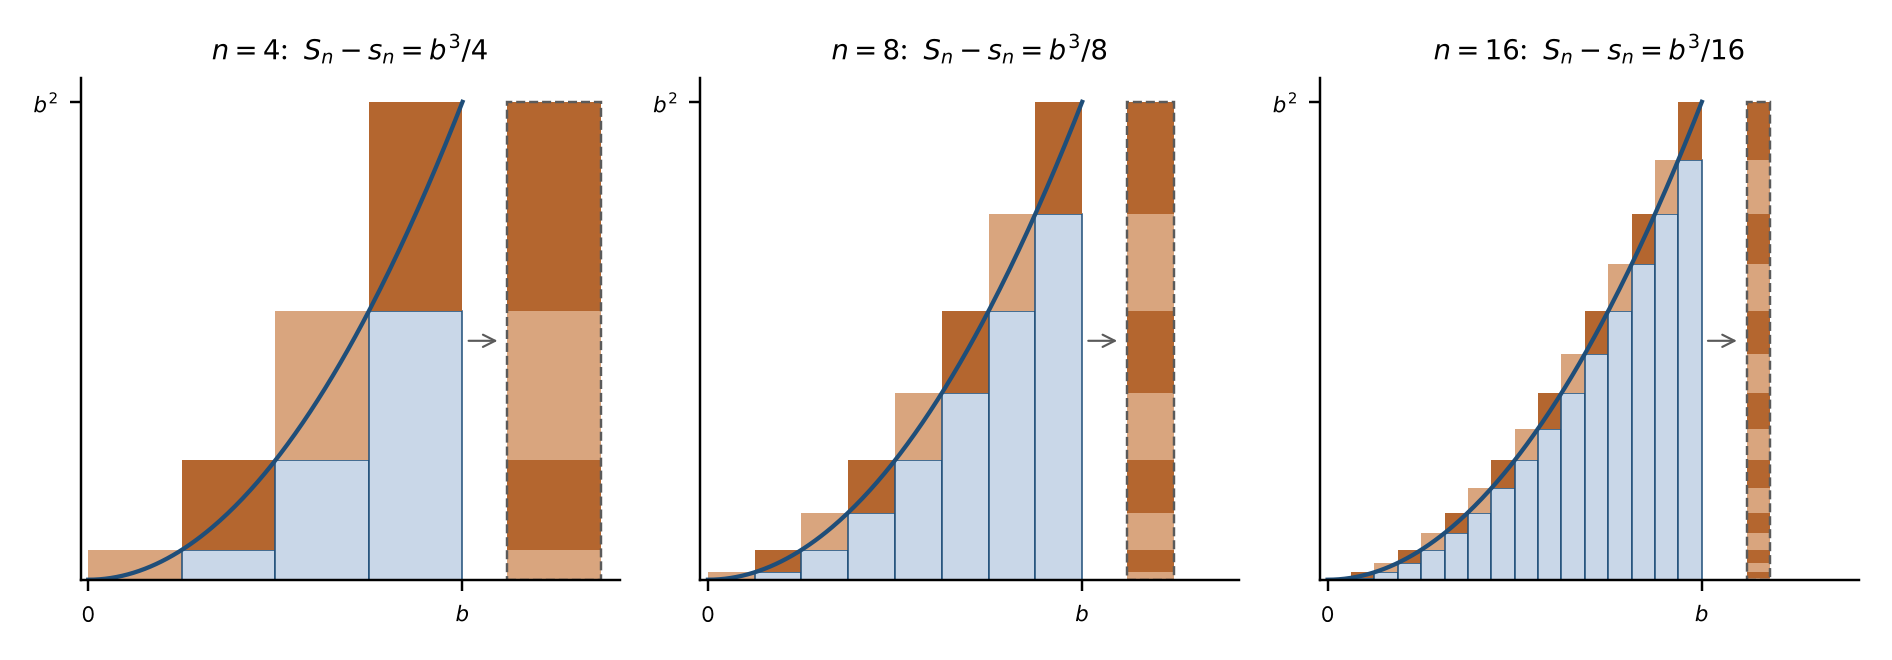
\includegraphics[width=\textwidth]{figure/esaustione.png}
\caption{La differenza $S_{n}-s_{n}=b^{3}/n$ per $n=4,8,16$. I rettangolini in color rame
(la parte di plurirettangolo circoscritto che eccede quello inscritto) si possono
traslare nell'ultima colonna, dove formano il rettangolo tratteggiato di base $b/n$ e
altezza $b^{2}$: la differenza vale esattamente $b^{3}/n$
(\texttt{python/fig\_esaustione.py}).}
\label{fig:telescopica}
\end{figure}

\needspace{12\baselineskip}
\subsection{L'area del settore di parabola}

\begin{proposizione}[Area del settore di parabola]\label{prop:settore-parabola}
Sia $b>0$ e siano $s_{n}$, $S_{n}$ le somme
\eqref{eq:somma-inferiore-parabola}--\eqref{eq:somma-superiore-parabola}. Allora
$b^{3}/3$ è l'\emph{unico} numero reale $c$ tale che
\begin{equation}\label{eq:separatore-parabola}
  s_{n}\le c\le S_{n} \qquad\perogni n\in\N .
\end{equation}
\end{proposizione}

\begin{schema}
\Ipotesi{$b>0$; \ $s_{n}$, $S_{n}$ somme inferiori e superiori di $x^{2}$ in $[0,b]$
relative alla suddivisione in $n$ parti uguali.}
\Tesi{(i) $s_{n}<\frac{b^{3}}3<S_{n}$ per ogni $n$; \ (ii) se $s_{n}\le c\le S_{n}$ per ogni
$n$, allora $c=\frac{b^{3}}3$.}
\end{schema}

\begin{strategia}
Le formule \eqref{eq:Sn-parabola} e \eqref{eq:sn-parabola} sono esplicite: sviluppando i
prodotti, entrambe si scrivono come $\frac{b^{3}}3$ più o meno termini che contengono
$\frac1n$ e $\frac1{n^{2}}$, e un confronto di segni prova la (i). Per l'unicità basta
osservare che due numeri compresi tra $s_{n}$ e $S_{n}$ distano al più
$S_{n}-s_{n}=\frac{b^{3}}n$, quantità che, per la proprietà di Archimede, diventa più
piccola di qualsiasi numero positivo assegnato.
\end{strategia}

\begin{dimostrazione}
(i) Sviluppando i prodotti nelle \eqref{eq:Sn-parabola} e \eqref{eq:sn-parabola},
\[
\begin{aligned}
  S_{n}&=\frac{b^{3}}6\cdot\frac{2n^{2}+3n+1}{n^{2}}
  =\frac{b^{3}}3+\frac{b^{3}}{2n}+\frac{b^{3}}{6n^{2}},\\
  s_{n}&=\frac{b^{3}}6\cdot\frac{2n^{2}-3n+1}{n^{2}}
  =\frac{b^{3}}3-\frac{b^{3}}{6n^{2}}\,(3n-1) .
\end{aligned}
\]
La prima mostra che $S_{n}>\frac{b^{3}}3$; nella seconda $3n-1>0$ per ogni $n\ge1$, e
quindi $s_{n}<\frac{b^{3}}3$.

(ii) Sia $c$ un numero che verifica la \eqref{eq:separatore-parabola}. Poiché anche
$\frac{b^{3}}3$ la verifica, i due numeri appartengono entrambi all'intervallo
$[s_{n},S_{n}]$, e quindi, per la \eqref{eq:differenza-parabola},
\[
  \Bigl|c-\frac{b^{3}}3\Bigr|\le S_{n}-s_{n}=\frac{b^{3}}n \qquad\perogni n\in\N .
\]
Se fosse $c\neq\frac{b^{3}}3$, per la proprietà di Archimede (\cref{teo:archimede})
esisterebbe $n\in\N$ con $n\,\bigl|c-\frac{b^{3}}3\bigr|>b^{3}$, contro la disuguaglianza
appena scritta. Dunque $c=\frac{b^{3}}3$.
\end{dimostrazione}

Dalle \eqref{eq:stime-parabola} e dalla proposizione segue che, se il settore $S$ ha
un'area, essa non può che essere
\begin{equation}\label{eq:area-parabola}
  \text{area }S=\frac{b^{3}}3 ,
\end{equation}
cioè \emph{un terzo} dell'area del rettangolo $[0,b]\times[0,b^{2}]$ che lo contiene.
È il risultato di Archimede. Allo stesso valore si arriva passando al limite nelle
\eqref{eq:Sn-parabola}--\eqref{eq:sn-parabola} (basta dividere numeratore e denominatore
per $n^{2}$): $s_{n}\to\frac{b^{3}}3$ e $S_{n}\to\frac{b^{3}}3$. Le due strade sono
equivalenti, ma la prima, che caratterizza l'area come \emph{unico elemento separatore}
tra le stime per difetto e quelle per eccesso, è quella che generalizzeremo.

Il programma seguente calcola le somme in aritmetica razionale esatta, con il modulo
\texttt{fractions}, per $b=1$: si vede la differenza $S_{n}-s_{n}=\frac1n$ e
l'avvicinamento di entrambe le somme a $\frac13$.

\begin{python}[Somme integrali del settore di parabola in aritmetica esatta]
from fractions import Fraction as F

def somme(n, b=F(1)):
    """Somme inferiore e superiore di x^2 in [0, b], n intervalli."""
    x = [F(k, n) * b for k in range(n + 1)]
    s = sum(x[k - 1]**2 * (x[k] - x[k - 1]) for k in range(1, n + 1))
    S = sum(x[k]**2 * (x[k] - x[k - 1]) for k in range(1, n + 1))
    return s, S

print(f"{'n':>5} {'s_n':>10} {'S_n':>10} {'S_n - s_n':>10}")
for n in (1, 2, 5, 10, 100, 1000):
    s, S = somme(n)
    print(f"{n:5d} {float(s):10.6f} {float(S):10.6f}"
          f" {float(S - s):10.6f}")
s, S = somme(10)
print("n = 10, valori esatti:", s, "< 1/3 <", S)
\end{python}
\begin{risultato}
    n        s_n        S_n  S_n - s_n
    1   0.000000   1.000000   1.000000
    2   0.125000   0.625000   0.500000
    5   0.240000   0.440000   0.200000
   10   0.285000   0.385000   0.100000
  100   0.328350   0.338350   0.010000
 1000   0.332834   0.333834   0.001000
n = 10, valori esatti: 57/200 < 1/3 < 77/200
\end{risultato}

\begin{osservazione}[Un indizio del teorema fondamentale]\label{oss:indizio-tfc}
Pensiamo l'area \eqref{eq:area-parabola} come funzione dell'estremo $b$ e deriviamola:
\begin{equation}\label{eq:derivata-area}
  \frac{d}{db}\Bigl(\frac{b^{3}}3\Bigr)=b^{2} .
\end{equation}
La derivata dell'area è il valore in $x=b$ della funzione $f(x)=x^{2}$ che delimita la
regione. Non è una coincidenza: se si sposta l'estremo da $b$ a $b+h$, l'area aumenta
di una striscia di base $h$ e altezza circa $b^{2}$, e il rapporto incrementale è
circa $b^{2}$. Questa osservazione, resa rigorosa, è il \emph{teorema fondamentale del
calcolo integrale}, che dimostreremo nel prossimo capitolo e che trasformerà il
calcolo delle aree in un problema di derivate.
\end{osservazione}

\begin{idea}[La teoria delle strisce e la portanza di un'ala]
Lungo l'apertura alare la portanza non è distribuita uniformemente: si descrive con la
\emph{portanza per unità di apertura} $l(y)$, misurata in N/m, dove $y\in[-\frac b2,
\frac b2]$ è la coordinata lungo l'apertura $b$. La portanza totale è l'«area» sotto il
grafico di $l$: per calcolarla, la \emph{teoria delle strisce} divide l'ala in strisce
di larghezza $\Delta y$ e somma i contributi $l(y_{k})\,\Delta y$, esattamente come
abbiamo fatto per la parabola. Un caso fondamentale è la \emph{distribuzione
ellittica}
\begin{equation}\label{eq:portanza-ellittica}
  l(y)=l_{0}\sqrt{1-\Bigl(\frac{2y}b\Bigr)^{2}}, \qquad -\frac b2\le y\le\frac b2,
\end{equation}
che, secondo la teoria della linea portante di Ludwig Prandtl (1918), rende minima la
resistenza indotta a parità di portanza e di apertura; la si ottiene, ad esempio, con
un'ala di pianta ellittica come quella dello Spitfire (\cref{fig:portanza-ellittica}).
Poiché $l$ è crescente in $[-\frac b2,0]$ e decrescente in $[0,\frac b2]$, se lo zero è
un estremo delle strisce, in ogni striscia il minimo e il massimo di $l$ sono assunti
negli estremi della striscia, e le somme per difetto e per eccesso si calcolano
facilmente. Vedremo nell'\cref{es:portanza-ellittica-esatta} che l'area sotto la
\eqref{eq:portanza-ellittica} vale $\frac\pi4l_{0}b$; per un velivolo di peso
$W=10\,000$~N e apertura $b=10$~m, il volo livellato ($L=W$) richiede dunque
$l_{0}=\frac{4W}{\pi b}\approx1273$~N/m.
\end{idea}

\begin{python}[Portanza totale con la teoria delle strisce]
import math

b, W = 10.0, 10000.0                  # apertura [m], peso [N]
l0 = 4 * W / (math.pi * b)            # carico al centro [N/m]

def l(y):
    """Portanza per unità di apertura, distribuzione ellittica."""
    return l0 * math.sqrt(max(0.0, 1 - (2 * y / b)**2))

def strisce(n):
    """Somme per difetto e per eccesso con n strisce (n pari)."""
    y = [-b / 2 + k * b / n for k in range(n + 1)]
    s = S = 0.0
    for k in range(1, n + 1):
        lo, hi = sorted((l(y[k - 1]), l(y[k])))  # l monotona
        s += lo * (y[k] - y[k - 1])
        S += hi * (y[k] - y[k - 1])
    return s, S

print(f"l0 = {l0:.2f} N/m")
for n in (4, 16, 64, 256, 1024):
    s, S = strisce(n)
    print(f"n = {n:4d}: {s:8.1f} N <= L <= {S:8.1f} N"
          f"   (S - s = {S - s:6.1f} N)")
\end{python}
\begin{risultato}
l0 = 1273.24 N/m
n =    4:   5513.3 N <= L <=  11879.5 N   (S - s = 6366.2 N)
n =   16:   9039.4 N <= L <=  10631.0 N   (S - s = 1591.5 N)
n =   64:   9780.4 N <= L <=  10178.3 N   (S - s =  397.9 N)
n =  256:   9947.7 N <= L <=  10047.2 N   (S - s =   99.5 N)
n = 1024:   9987.2 N <= L <=  10012.1 N   (S - s =   24.9 N)
\end{risultato}

\begin{figure}[htb]
\centering
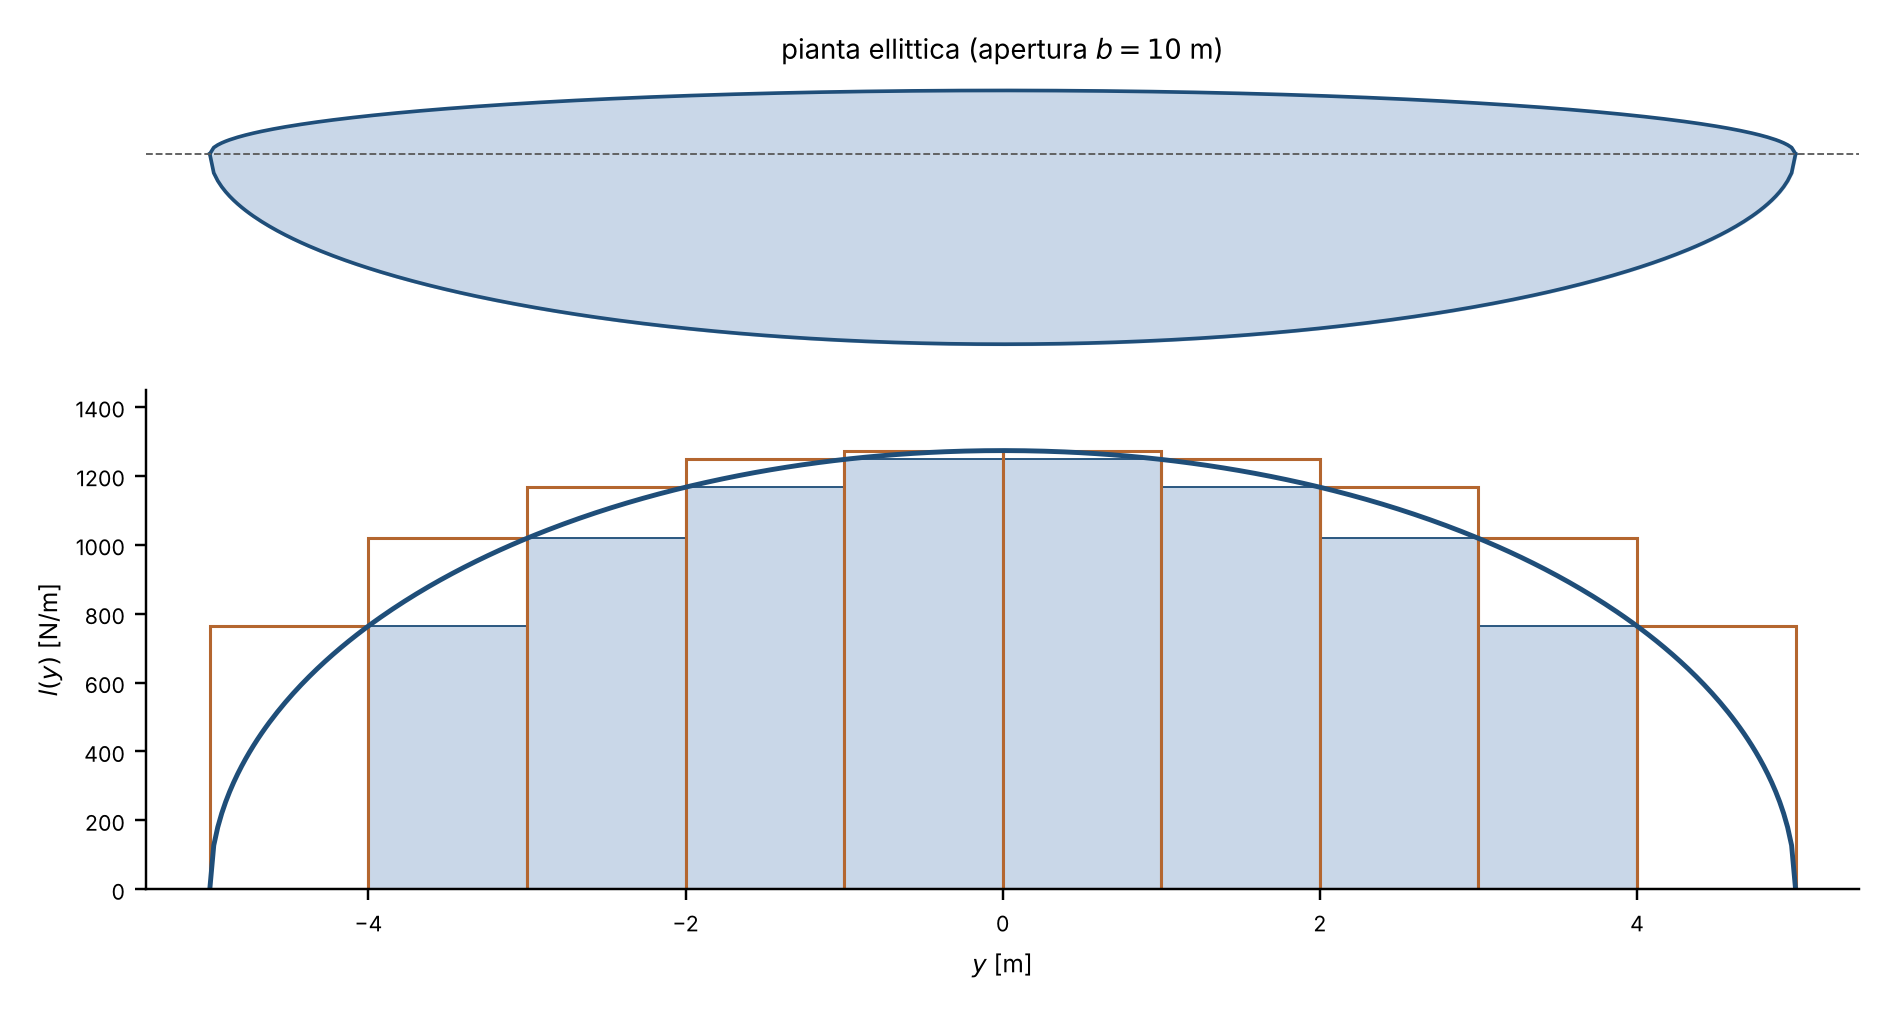
\includegraphics[width=\textwidth]{figure/portanza_ellittica.png}
\caption{In alto, la pianta ellittica di un'ala di apertura $b=10$~m. In basso, la
distribuzione ellittica della portanza \eqref{eq:portanza-ellittica} con $10$ strisce:
in azzurro i rettangoli della somma per difetto, in color rame il contorno di quelli
della somma per eccesso (\texttt{python/fig\_portanza\_ellittica.py}).}
\label{fig:portanza-ellittica}
\end{figure}

Anche qui la differenza tra le due somme è telescopica: in ciascuna delle due metà
dell'ala, dove $l$ è monotòna e passa dal valore $0$ al valore $l_{0}$, essa vale
$\frac{l_{0}b}n$, e in totale $S-s=\frac{2l_{0}b}n$. Le somme convergono al valore
esatto $10\,000$~N, ma lentamente, come $1/n$: nel \cref{sec:integrabilita-continue}
vedremo formule di approssimazione molto più efficienti.

\begin{notastorica}[Da Eudosso a Fermat]
Eudosso di Cnido (circa 408--355 a.C.) è considerato l'inventore del metodo di
esaustione, con il quale dimostrò, ad esempio, che il volume di un cono è un terzo di
quello del cilindro con la stessa base e la stessa altezza. Archimede di Siracusa
(circa 287--212 a.C.) ne fece uno strumento potentissimo: nella \emph{Quadratura della
parabola} dimostrò che il segmento parabolico ha un'area uguale ai $\frac43$ di quella
del triangolo inscritto con la stessa base e lo stesso vertice (ne seguiremo il
ragionamento nel \S\ref{subsec:archimede-parabola}). L'esaustione restò per due
millenni il modello del rigore, ma andava reinventata per ogni figura; nel Seicento si
cercarono scorciatoie. Keplero, nella \emph{Nova stereometria doliorum vinariorum}
(1615), vide il cerchio come formato da infiniti triangolini con il vertice nel centro.
Bonaventura Cavalieri, allievo di Galileo, nella \emph{Geometria indivisibilibus
continuorum} (1635) trattò le figure piane come insiemi di infinite corde parallele, gli
\emph{indivisibili}, e ne ricavò il \emph{principio di Cavalieri}: due figure tagliate da
ogni parallela a una retta data secondo corde uguali hanno la stessa area. Evangelista
Torricelli, nell'\emph{Opera geometrica} (1644), diede una ventina di dimostrazioni del
teorema di Archimede, alcune alla maniera degli antichi, altre con gli indivisibili.
John Wallis, nell'\emph{Arithmetica infinitorum} (1656), osservò che il rapporto tra
$0^{2}+1^{2}+\dots+n^{2}$ e $(n+1)\,n^{2}$ vale $\frac13+\frac1{6n}$, e ne concluse che
«all'infinito» esso diventa $\frac13$: è la \eqref{eq:area-parabola}. Pierre de Fermat,
negli stessi anni, calcolò l'area sotto le curve $y=x^{n}$ suddividendo l'intervallo
con punti in progressione geometrica. Questi metodi guadagnavano in generalità ciò che perdevano in rigore; le
somme integrali di questo capitolo conservano l'una e l'altro.
\end{notastorica}

\subsection{Approfondimento: la quadratura della parabola di Archimede}
\label{subsec:archimede-parabola}

Archimede non usò rettangoli, ma «esaurì» il segmento di parabola con triangoli:
inscrisse nel segmento un triangolo, nei due segmenti rimasti scoperti altri due
triangoli, e così via. Seguiamo il suo ragionamento sulla parabola $y=x^{2}$, con le
coordinate, che Archimede non aveva. Come nel \cref{sec:esaustione}, attribuiamo
all'area le proprietà suggerite dall'intuizione (aree elementari, additività per figure
senza punti interni comuni, confronto per inclusione); non useremo né limiti né serie,
ma soltanto una somma finita e la proprietà di Archimede.

Siano $p<r$ e siano $A=(p,p^{2})$, $B=(r,r^{2})$ due punti della parabola. La retta
$AB$ ha equazione $y=c(x)$, con $c(x)=(p+r)x-pr$, come si verifica sostituendo $x=p$ e
$x=r$. Chiamiamo \emph{segmento parabolico} di corda $AB$ la regione
\begin{equation}\label{eq:segmento-parabolico}
  \Sigma(p,r)=\set{(x,y)\in\R^{2} \tc p\le x\le r,\ \ x^{2}\le y\le c(x)} ,
\end{equation}
compresa tra l'arco di parabola e la corda, e \emph{triangolo di Archimede} del segmento
il triangolo $ABC$, dove $C=(q,q^{2})$ è il punto della parabola di ascissa
$q=\frac{p+r}2$ (\cref{fig:archimede-parabola}, a sinistra).

\begin{lemma}[Il triangolo di Archimede]\label{lem:triangolo-archimede}
Siano $p<r$, $w=r-p$, $q=\frac{p+r}2$, e sia $t(x)=(p+r)x-q^{2}$ la retta per $C$
parallela alla corda. Allora:
\begin{enumerate}[label=\textup{(\alph*)}]
  \item $t(x)\le x^{2}\le c(x)$ per ogni $x\in[p,r]$;
  \item il triangolo $ABC$ ha area $\frac{w^{3}}8$;
  \item il segmento $\Sigma(p,r)$ è contenuto nel parallelogramma delimitato dalle rette
  $y=c(x)$, $y=t(x)$, $x=p$, $x=r$, che ha area $\frac{w^{3}}4$, doppia di quella del
  triangolo.
\end{enumerate}
\end{lemma}

\begin{schema}
\Ipotesi{$p<r$; \ $A$, $B$, $C$ punti della parabola $y=x^{2}$ di ascisse $p$, $r$,
$q=\frac{p+r}2$.}
\Tesi{(a) $t\le x^{2}\le c$ in $[p,r]$; \ (b) area $ABC=\frac{(r-p)^{3}}8$; \
(c) $\Sigma(p,r)$ sta in un parallelogramma di area doppia di quella di $ABC$.}
\end{schema}

\begin{strategia}
Tutto si riduce a due fattorizzazioni: $c(x)-x^{2}=(x-p)(r-x)$ e
$x^{2}-t(x)=(x-q)^{2}$. La prima dice che l'arco sta sotto la corda, la seconda che sta
sopra la parallela per $C$, cioè che questa è la tangente in $C$. Per l'area del
triangolo lo si taglia con la verticale per $C$, che lo divide in due triangoli con un
lato verticale comune.
\end{strategia}

\begin{dimostrazione}
(a) Sviluppando i prodotti si verifica che $c(x)-x^{2}=-x^{2}+(p+r)x-pr=(x-p)(r-x)$,
che è non negativo per $p\le x\le r$. Inoltre, poiché $p+r=2q$,
$x^{2}-t(x)=x^{2}-2qx+q^{2}=(x-q)^{2}\ge0$ per ogni $x$: la retta $y=t(x)$, la cui
pendenza $2q$ è la derivata di $x^{2}$ in $q$, tocca la parabola soltanto in $C$.

(b) Sia $D=(q,c(q))$ il punto della corda sulla verticale per $C$. Per la (a), la
lunghezza del segmento $CD$ è
\[
  d=c(q)-q^{2}=(q-p)(r-q)=\frac w2\cdot\frac w2=\frac{w^{2}}4 .
\]
Il segmento $CD$ divide il triangolo $ABC$ nei triangoli $ACD$ e $DCB$, che hanno $CD$
come lato comune e altezze relative a esso uguali alle distanze orizzontali $q-p=\frac
w2$ e $r-q=\frac w2$. Dunque l'area di $ABC$ è
$\frac12\,d\,\frac w2+\frac12\,d\,\frac w2=\frac{dw}2=\frac{w^{3}}8$.

(c) Se $(x,y)\in\Sigma(p,r)$, allora $p\le x\le r$ e, per la (a),
$t(x)\le x^{2}\le y\le c(x)$: il punto appartiene al parallelogramma descritto
nell'enunciato. Le rette $y=c(x)$ e $y=t(x)$ hanno la stessa pendenza, quindi la
distanza verticale tra esse è costante e vale $c(q)-t(q)=c(q)-q^{2}=d$. Il
parallelogramma ha due lati verticali di lunghezza $d$ a distanza $w$, e la sua area è
$dw=\frac{w^{3}}4$, il doppio dell'area del triangolo.
\end{dimostrazione}

\begin{figure}[htb]
\centering
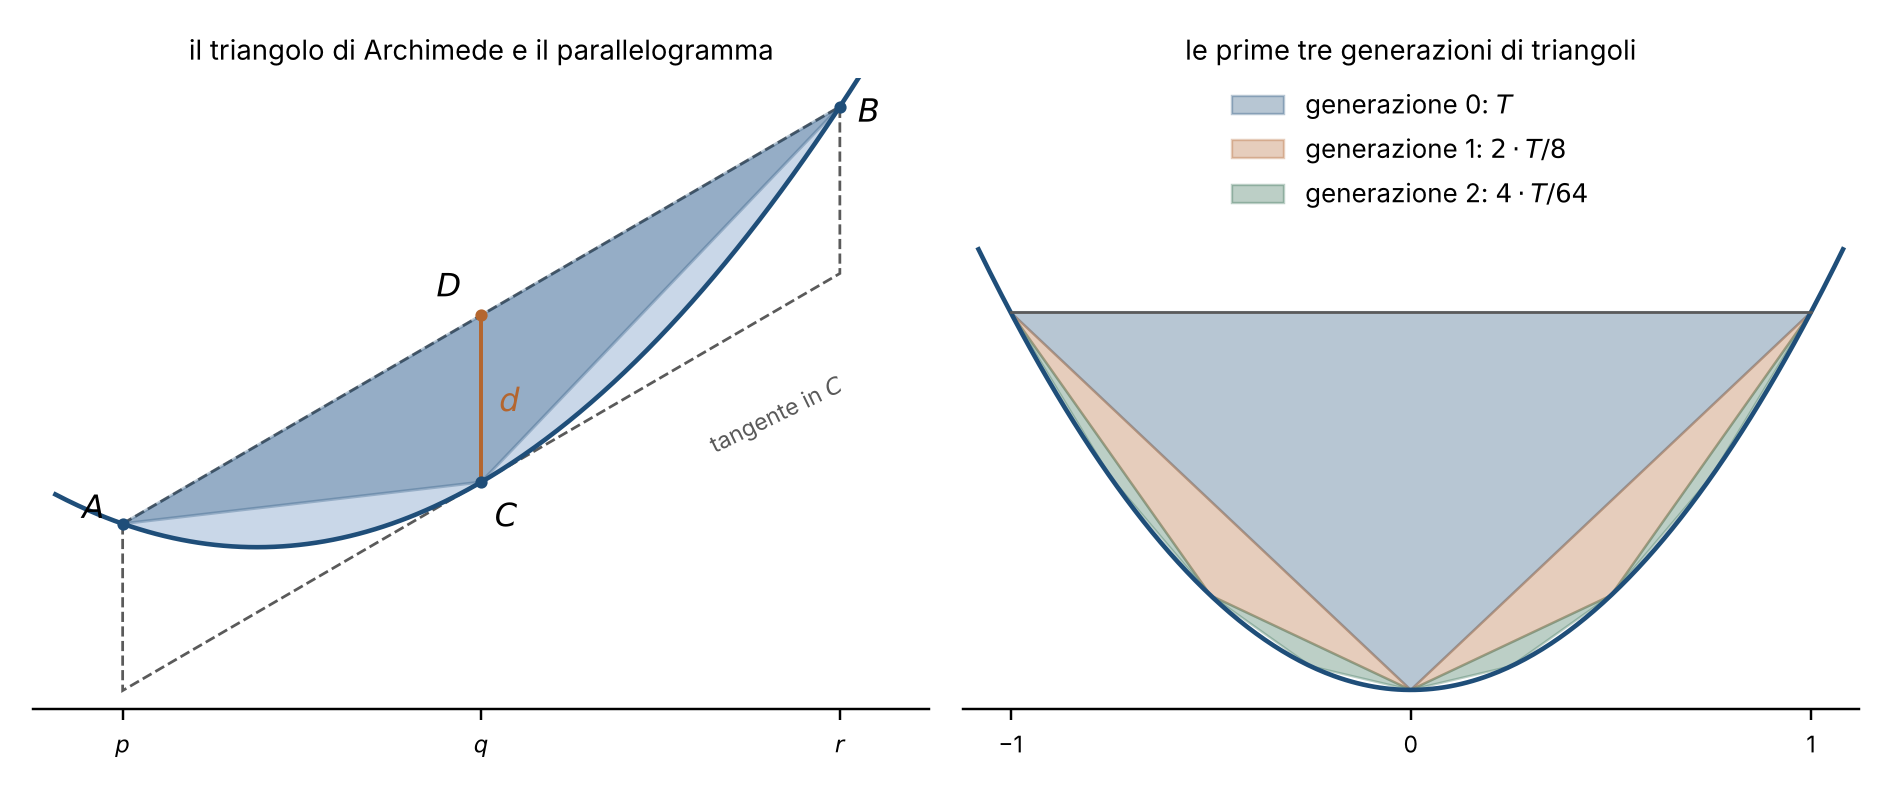
\includegraphics[width=\textwidth]{figure/archimede_parabola.png}
\caption{A sinistra, il segmento parabolico $\Sigma(p,r)$ (azzurro chiaro), il suo
triangolo di Archimede $ABC$ e il parallelogramma tratteggiato del
\cref{lem:triangolo-archimede}, delimitato dalla corda e dalla tangente in $C$, che
contiene il segmento e ha area doppia di quella del triangolo. A destra, i triangoli
delle prime tre generazioni per la corda di estremi $(\pm1,1)$: ogni generazione ha
area totale pari a $\frac14$ della precedente
(\texttt{python/fig\_archimede\_parabola.py}).}
\label{fig:archimede-parabola}
\end{figure}

\needspace{10\baselineskip}
Il segmento $\Sigma(p,r)$ si scompone nel triangolo $ABC$ e nei due segmenti
$\Sigma(p,q)$ e $\Sigma(q,r)$, di corde $AC$ e $CB$, senza punti interni comuni: per
$p\le x\le q$, ad esempio, la corda $AC$ divide il segmento verticale di $\Sigma(p,r)$
sopra $x$ in una parte che sta in $\Sigma(p,q)$ e una che sta nel triangolo. I due nuovi
segmenti hanno corde di larghezza $\frac w2$ e, per il lemma, triangoli di Archimede di
area $\frac18\cdot\frac{w^{3}}8$ ciascuno: insieme, un quarto del primo triangolo. È il
motore della dimostrazione.

\begin{proposizione}[Quadratura della parabola]\label{prop:quadratura-archimede}
Siano $p<r$ e sia $T=\frac{(r-p)^{3}}8$ l'area del triangolo di Archimede del segmento
parabolico $\Sigma(p,r)$. Se il segmento ha un'area, essa vale
\begin{equation}\label{eq:quadratura-archimede}
  \text{area }\Sigma(p,r)=\frac43\,T=\frac{(r-p)^{3}}6 .
\end{equation}
\end{proposizione}

\begin{schema}
\Ipotesi{$p<r$; \ l'area gode delle proprietà intuitive (aree elementari, additività,
confronto per inclusione).}
\Tesi{area $\Sigma(p,r)=\frac43\,T$, \ dove $T=\frac{(r-p)^{3}}8$ è l'area del
triangolo di Archimede.}
\end{schema}

\begin{strategia}
Si inscrivono nel segmento triangoli di generazioni successive: ogni generazione ha
area totale $\frac14$ della precedente, e l'unione delle prime $n+1$ generazioni è un
poligono la cui area è una somma geometrica finita, minore di $\frac43T$ per
$\frac T{3\cdot4^{n}}$. Ciò che resta scoperto è formato da segmenti più piccoli, e per
il \cref{lem:triangolo-archimede}(c) ha area al più doppia di quella della generazione
successiva. Archimede conclude con una \emph{doppia riduzione all'assurdo}: l'area del
segmento non può essere né maggiore né minore di $\frac43T$.
\end{strategia}

\begin{dimostrazione}
Sia $w=r-p$. Per $k\ge0$ intero, i punti $x_{j}=p+j\frac w{2^{k}}$,
$j=0,\dots,2^{k}$, dividono $[p,r]$ in $2^{k}$ parti uguali; chiamiamo \emph{segmenti di
generazione $k$} i $2^{k}$ segmenti parabolici $\Sigma(x_{j-1},x_{j})$, di corde di
larghezza $\frac w{2^{k}}$. Per il \cref{lem:triangolo-archimede}(b), ciascuno di essi
ha un triangolo di Archimede di area $\frac18\bigl(\frac w{2^{k}}\bigr)^{3}=\frac
T{8^{k}}$, e i triangoli di generazione $k$ hanno area totale
$2^{k}\cdot\frac T{8^{k}}=\frac T{4^{k}}$. Per la scomposizione descritta prima
dell'enunciato, ogni segmento di generazione $k$ è l'unione del suo triangolo e di due
segmenti di generazione $k+1$, senza punti interni comuni. Ripetendo la scomposizione,
per ogni $n\in\N$ il segmento $\Sigma(p,r)$ è l'unione del poligono $P_{n}$, formato dai
triangoli delle generazioni $0,1,\dots,n$, e dei $2^{n+1}$ segmenti di generazione
$n+1$, senza punti interni comuni.

\emph{L'area del poligono.} Per l'additività e per la somma della progressione
geometrica (\cref{prop:geometrica}) con $x=\frac14$,
\begin{equation}\label{eq:poligono-archimede}
  \text{area }P_{n}=T\Bigl(1+\frac14+\dots+\frac1{4^{n}}\Bigr)
  =T\,\frac{1-\frac1{4^{n+1}}}{1-\frac14}=\frac43\,T-\frac T{3\cdot4^{n}} .
\end{equation}

\emph{Ciò che resta scoperto.} Per il \cref{lem:triangolo-archimede}(c) e il confronto
per inclusione, ogni segmento di generazione $n+1$ ha area minore o uguale del doppio
del suo triangolo, cioè di $\frac{2T}{8^{n+1}}$. Sommando sui $2^{n+1}$ segmenti, la parte
scoperta $R_{n}=\text{area }\Sigma(p,r)-\text{area }P_{n}$ verifica
\begin{equation}\label{eq:resto-archimede}
  R_{n}\le2^{n+1}\cdot\frac{2T}{8^{n+1}}=\frac{2T}{4^{n+1}}=\frac T{2\cdot4^{n}} .
\end{equation}

\emph{La doppia riduzione all'assurdo.} Poniamo $\mathcal A=\text{area }\Sigma(p,r)$ e
$K=\frac43T$. Osserviamo che $4^{n}=(1+3)^{n}\ge1+3n>n$ per la disuguaglianza di
Bernoulli (\cref{teo:bernoulli}). Se fosse $\mathcal A>K$, per la proprietà di
Archimede (\cref{teo:archimede}) esisterebbe $n\in\N$ con $n>\frac T{2(\mathcal A-K)}$;
per la \eqref{eq:resto-archimede} si avrebbe $R_{n}\le\frac T{2\cdot4^{n}}<\frac T{2n}
<\mathcal A-K$, cioè $\text{area }P_{n}=\mathcal A-R_{n}>K$, contro la
\eqref{eq:poligono-archimede}, che dà $\text{area }P_{n}<K$. Se fosse $\mathcal A<K$,
esisterebbe $n\in\N$ con $n>\frac T{3(K-\mathcal A)}$, e per la
\eqref{eq:poligono-archimede} $K-\text{area }P_{n}=\frac T{3\cdot4^{n}}<\frac T{3n}<
K-\mathcal A$, cioè $\text{area }P_{n}>\mathcal A$: impossibile, perché il poligono $P_{n}$
è contenuto nel segmento. Esclusi i due casi, resta $\mathcal A=K=\frac43T$, e
$\frac43\cdot\frac{(r-p)^{3}}8=\frac{(r-p)^{3}}6$.
\end{dimostrazione}

\begin{osservazione}[La somma di Archimede e la serie geometrica]
\label{oss:somma-archimede}
Archimede ottenne la \eqref{eq:poligono-archimede} con una somma telescopica: ogni
termine, aumentato di un suo terzo, è un terzo del precedente,
$\frac1{4^{k}}+\frac13\cdot\frac1{4^{k}}=\frac13\cdot\frac1{4^{k-1}}$, e sommando per
$k=1,\dots,n$ si ha $1+\frac14+\dots+\frac1{4^{n}}+\frac13\cdot\frac1{4^{n}}=\frac43$.
Nel linguaggio del \cref{cap:serie}, la serie geometrica $1+\frac14+\frac1{16}+\cdots$
ha somma $\frac43$: la doppia riduzione all'assurdo fa le veci del passaggio al limite.
\end{osservazione}

\begin{esempio}[Due verifiche con il settore di parabola]\label{es:archimede-settore}
Per la corda di estremi $(\pm b,b^{2})$ la \eqref{eq:quadratura-archimede} dà
$\frac{(2b)^{3}}6=\frac43b^{3}$; con la \eqref{eq:area-parabola}, il segmento è il
rettangolo $[-b,b]\times[0,b^{2}]$ privato di due regioni congruenti al settore
\eqref{eq:settore-parabola}, e ha area $2b^{3}-2\cdot\frac{b^{3}}3=\frac43b^{3}$. Per la
corda di estremi $(0,0)$ e $(b,b^{2})$ si ottiene $\frac{b^{3}}6$, e infatti togliendo
il settore $S$ dal triangolo di vertici $(0,0)$, $(b,0)$, $(b,b^{2})$ resta
$\frac{b^{3}}2-\frac{b^{3}}3=\frac{b^{3}}6$. I triangoli di Archimede e i rettangoli
delle somme integrali portano allo stesso risultato.
\end{esempio}

\begin{notastorica}[Il \emph{Metodo} di Archimede]
La \emph{Quadratura della parabola}, indirizzata all'astronomo Dositeo di Pelusio,
contiene due dimostrazioni del teorema dei $\frac43$: una «meccanica», che equilibra il
segmento con un triangolo su una bilancia ideale, e quella con i triangoli inscritti che
abbiamo appena seguito. Entrambe, però, presuppongono di conoscere il risultato:
l'esaustione è un metodo di dimostrazione, non di scoperta, e già nel Seicento si
sospettava che Archimede possedesse un procedimento segreto per trovare i suoi teoremi.
La risposta arrivò nel 1906, quando il filologo danese Johan Ludvig Heiberg riconobbe, in
un libro di preghiere conservato a Costantinopoli, il testo raschiato di un codice di
opere di Archimede copiato nel \textsc{x} secolo, la cui pergamena era stata riutilizzata
nel 1229. Vi si trovava, in copia unica, il \emph{Metodo sui teoremi meccanici}, una
lettera a Eratostene in cui Archimede racconta di aver scoperto i suoi risultati
scomponendo le figure in infinite strisce parallele e bilanciandole su una leva, e
avverte che questo modo di ragionare suggerisce la verità ma non la dimostra. Il primo
esempio della lettera è proprio il segmento di parabola. Rimasto a lungo irreperibile,
il palinsesto ricomparve a un'asta nel 1998 ed è stato poi studiato a Baltimora con
tecniche di imaging multispettrale, che hanno restituito passi che Heiberg non era
riuscito a leggere. Le strisce del \emph{Metodo} sono le antenate degli indivisibili di
Cavalieri e dei rettangoli delle nostre somme integrali.
\end{notastorica}

%% ----------------------------------------------------------------------------
%%  §8.2  Somme integrali e integrale definito
%% ----------------------------------------------------------------------------
\section{Somme integrali e integrale definito}
\label{sec:integrale-definito}

Generalizziamo il procedimento del paragrafo precedente a una funzione qualsiasi,
purché \emph{limitata}. In tutto il paragrafo $[a,b]$ è un intervallo chiuso e limitato,
con $a<b$, e $f:[a,b]\to\R$ è una funzione limitata: esistono due costanti $m$, $M$ tali
che
\begin{equation}\label{eq:f-limitata}
  m\le f(x)\le M \qquad\perogni x\in[a,b] .
\end{equation}
Rispetto al settore di parabola cambiano due cose. La suddivisione dell'intervallo non
sarà più necessariamente in parti uguali; e, poiché $f$ non è più monotòna, l'altezza
dei rettangoli inscritti e circoscritti non sarà più il valore di $f$ in un estremo,
ma l'estremo inferiore e l'estremo superiore di $f$ nell'intervallo.

\subsection{Partizioni e somme integrali}

\begin{definizione}[Partizione]\label{def:partizione}\index{partizione}
Si chiama \emph{partizione} dell'intervallo $[a,b]$ un insieme finito
$P=\set{x_{0},x_{1},\dots,x_{n}}$ di punti, con $n\in\N$, tali che
\begin{equation}\label{eq:partizione}
  a=x_{0}<x_{1}<\dots<x_{k-1}<x_{k}<\dots<x_{n}=b .
\end{equation}
Gli $n+1$ punti individuano $n$ intervalli $I_{k}=[x_{k-1},x_{k}]$, $k=1,\dots,n$, di
ampiezza $\Delta x_{k}=x_{k}-x_{k-1}$. Il numero $\abs P=\max_{k}\Delta x_{k}$ si chiama
\emph{ampiezza} della partizione. Se $P$ e $Q$ sono partizioni di $[a,b]$ e
$P\subseteq Q$, si dice che $Q$ è \emph{più fine} di $P$, o che è un
\emph{raffinamento} di $P$.
\end{definizione}

Le ampiezze degli intervalli hanno per somma la lunghezza dell'intervallo:
$\sum_{k=1}^{n}\Delta x_{k}=x_{n}-x_{0}=b-a$ (ancora una somma telescopica). L'esempio
più semplice è la \emph{partizione uniforme} in $n$ parti uguali, con
$x_{k}=a+k\frac{b-a}n$ e $\abs P=\frac{b-a}n$, che abbiamo usato nel paragrafo
precedente. Se $P$ e $Q$ sono due partizioni di $[a,b]$, l'insieme
\begin{equation}\label{eq:unione-partizioni}
  R=P\cup Q ,
\end{equation}
ottenuto prendendo insieme i punti di $P$ e quelli di $Q$ (e ordinandoli), è ancora una
partizione di $[a,b]$, più fine sia di $P$ sia di $Q$.

\begin{definizione}[Somme integrali]\label{def:somme-integrali}\index{somma integrale}
Sia $P=\set{x_{0},\dots,x_{n}}$ una partizione di $[a,b]$. Per $k=1,\dots,n$ poniamo
\begin{equation}\label{eq:mk-Mk}
\begin{aligned}
  m_{k}&=\inf\set{f(x) \tc x\in[x_{k-1},x_{k}]},\\
  M_{k}&=\sup\set{f(x) \tc x\in[x_{k-1},x_{k}]} .
\end{aligned}
\end{equation}
Si chiamano \emph{somma integrale inferiore} e \emph{somma integrale superiore} di $f$
relative a $P$ i numeri
\begin{equation}\label{eq:somme-integrali}
  s(P)=\sum_{k=1}^{n}m_{k}\,(x_{k}-x_{k-1}), \qquad
  S(P)=\sum_{k=1}^{n}M_{k}\,(x_{k}-x_{k-1}) .
\end{equation}
Quando occorre ricordare la funzione si scrive $s(P,f)$ e $S(P,f)$.
\end{definizione}

Gli estremi $m_{k}$ e $M_{k}$ esistono finiti per il \cref{teo:esistenza-sup}, perché
l'insieme dei valori di $f$ in $[x_{k-1},x_{k}]$ è non vuoto e limitato; inoltre, per la
\eqref{eq:f-limitata}, $m\le m_{k}\le M_{k}\le M$. Moltiplicando per $\Delta x_{k}>0$ e
sommando si ottiene la stima
\begin{equation}\label{eq:stime-somme}
  m(b-a)\le s(P)\le S(P)\le M(b-a) \qquad\text{per ogni partizione } P .
\end{equation}
Se $f\ge0$, le somme integrali hanno il chiaro significato geometrico di somme delle
aree dei rettangoli rispettivamente inscritti nella regione sotto il grafico e
circoscritti a essa (\cref{fig:somme-integrali}). Si noti però che $s(P)$ e $S(P)$ sono
definite indipendentemente da ogni significato geometrico, anche se $f$ cambia segno.
Per $f(x)=x^{2}$ in $[0,b]$ e la partizione uniforme si ha $m_{k}=x_{k-1}^{2}$ e
$M_{k}=x_{k}^{2}$, e ritroviamo le somme $s_{n}$ e $S_{n}$ del \cref{sec:esaustione}.

\begin{figure}[htb]
\centering
\begin{tikzpicture}
\begin{axis}[width=0.9\textwidth, height=5.6cm, axis lines=left, xmin=0, xmax=4.95,
  ymin=0, ymax=3.1, xtick={0.3,1.3,2.5,3.3,4.5},
  xticklabels={$a=x_{0}$,$x_{1}$,$x_{2}$,$x_{3}$,$b=x_{4}$},
  ytick={1.345,2.424,2.733}, yticklabels={$m_{1}$,$m_{2}=M_{1}$,$M_{2}$},
  tick label style={font=\scriptsize}, clip=false]
  \fill[blu!20] (axis cs:0.3,0) rectangle (axis cs:1.3,1.345);
  \fill[blu!20] (axis cs:1.3,0) rectangle (axis cs:2.5,2.424);
  \fill[blu!20] (axis cs:2.5,0) rectangle (axis cs:3.3,1.899);
  \fill[blu!20] (axis cs:3.3,0) rectangle (axis cs:4.5,1.413);
  \draw[rame, thick] (axis cs:0.3,0) rectangle (axis cs:1.3,2.424);
  \draw[rame, thick] (axis cs:1.3,0) rectangle (axis cs:2.5,2.733);
  \draw[rame, thick] (axis cs:2.5,0) rectangle (axis cs:3.3,2.569);
  \draw[rame, thick] (axis cs:3.3,0) rectangle (axis cs:4.5,1.899);
  \addplot[curva, domain=0.2:4.65, samples=150] {1.7+0.8*sin(deg(1.3*x-0.9))+0.12*x};
  \addplot[tratteggio] coordinates {(0,1.345) (0.3,1.345)};
  \addplot[tratteggio] coordinates {(0,2.424) (1.3,2.424)};
  \addplot[tratteggio] coordinates {(0,2.733) (1.3,2.733)};
  \node[font=\scriptsize, blu, anchor=west] at (axis cs:4.67,1.53) {$y=f(x)$};
\end{axis}
\end{tikzpicture}
\caption{Somme integrali relative a una partizione non uniforme con $n=4$ intervalli.
L'area azzurra è la somma inferiore $s(P)$, quella racchiusa dai contorni in color rame
è la somma superiore $S(P)$. Nel secondo intervallo il massimo $M_{2}$ è assunto in un
punto interno, nel quarto il minimo $m_{4}$: le altezze dei rettangoli non sono, in
generale, i valori di $f$ negli estremi.}
\label{fig:somme-integrali}
\end{figure}

Il risultato seguente afferma che raffinando una partizione la somma inferiore
\emph{aumenta} (o resta uguale) e quella superiore \emph{diminuisce} (o resta uguale): le
due stime migliorano. Ne segue che \emph{ogni} somma inferiore è minore o uguale di
\emph{ogni} somma superiore, anche relativa a un'altra partizione.

\begin{lemma}[Raffinamento delle partizioni]\label{lem:raffinamento}
Siano $P$ e $Q$ partizioni di $[a,b]$.
\begin{enumerate}[label=\textup{(\alph*)}]
  \item Se $P\subseteq Q$, allora $s(P)\le s(Q)\le S(Q)\le S(P)$.
  \item In ogni caso, posto $R=P\cup Q$, risulta
  \begin{equation}\label{eq:s-minore-S}
    s(P)\le s(R)\le S(R)\le S(Q) .
  \end{equation}
\end{enumerate}
\end{lemma}

\begin{schema}
\Ipotesi{$f$ limitata in $[a,b]$; \ $P$, $Q$ partizioni di $[a,b]$.}
\Tesi{(a) $P\subseteq Q \implica s(P)\le s(Q)\le S(Q)\le S(P)$; \
(b) $s(P)\le S(Q)$ per ogni coppia $P$, $Q$.}
\end{schema}

\begin{strategia}
Il caso essenziale è quello in cui $Q$ ha un solo punto $\bar x$ in più di $P$. Allora
le due somme inferiori differiscono soltanto per i termini relativi all'intervallo di
$P$ che contiene $\bar x$, e tutto si riduce a un'osservazione sugli estremi inferiori:
l'estremo inferiore di $f$ su un insieme più piccolo è \emph{maggiore o uguale} di quello
sull'insieme più grande. Il caso generale si ottiene aggiungendo i punti di $Q$ uno alla
volta. La (b) segue dalla (a) applicata a $R$, che raffina sia $P$ sia $Q$.
\end{strategia}

\begin{dimostrazione}
(a) Supponiamo dapprima che $Q=P\cup\set{\bar x}$, con $x_{k-1}<\bar x<x_{k}$ per un certo
$k$, e poniamo
\[
  m'=\inf\set{f(x) \tc x\in[x_{k-1},\bar x]}, \qquad
  m''=\inf\set{f(x) \tc x\in[\bar x,x_{k}]} .
\]
Gli insiemi dei valori di $f$ in $[x_{k-1},\bar x]$ e in $[\bar x,x_{k}]$ sono contenuti
nell'insieme dei valori di $f$ in $[x_{k-1},x_{k}]$; poiché $m_{k}$ è un minorante di
quest'ultimo, è un minorante anche dei due sottoinsiemi, e quindi è minore o uguale dei
loro estremi inferiori: $m'\ge m_{k}$, $m''\ge m_{k}$. Le somme $s(Q)$ e $s(P)$ hanno in
comune tutti i termini tranne quelli relativi a $[x_{k-1},x_{k}]$, e dunque
\[
\begin{aligned}
  s(Q)-s(P)&=m'(\bar x-x_{k-1})+m''(x_{k}-\bar x)-m_{k}(x_{k}-x_{k-1})\\
  &\ge m_{k}\bigl[(\bar x-x_{k-1})+(x_{k}-\bar x)-(x_{k}-x_{k-1})\bigr]=0 .
\end{aligned}
\]
In modo analogo, gli estremi superiori sui due sottointervalli sono minori o uguali di
$M_{k}$, e si ottiene $S(Q)\le S(P)$. Se $Q$ contiene $p\ge2$ punti che non stanno in $P$,
si costruisce una catena $P=Q_{0}\subset Q_{1}\subset\dots\subset Q_{p}=Q$ in cui ciascuna
partizione si ottiene dalla precedente aggiungendo un solo punto; applicando il caso già
dimostrato a ogni anello della catena (cioè ragionando per induzione su $p$) si ottiene
$s(P)\le s(Q)$ e $S(Q)\le S(P)$. Infine $s(Q)\le S(Q)$ perché $m_{k}\le M_{k}$ per ogni
intervallo di $Q$.

(b) La partizione $R=P\cup Q$ è più fine sia di $P$ sia di $Q$. Applicando la (a) alla
coppia $P\subseteq R$ si ha $s(P)\le s(R)\le S(R)$, e applicandola alla coppia
$Q\subseteq R$ si ha $S(R)\le S(Q)$.
\end{dimostrazione}

\begin{figure}[htb]
\centering
\begin{tikzpicture}
\begin{axis}[width=0.62\textwidth, height=5cm, axis lines=left, xmin=0.4, xmax=4.1,
  ymin=0, ymax=4.3, xtick={1,2.4,3.6}, xticklabels={$x_{k-1}$,$\bar x$,$x_{k}$},
  ytick={0.85,2.04,3.84}, yticklabels={$m_{k}$,$m''=M'$,$M_{k}$},
  tick label style={font=\scriptsize}, clip=false]
  \fill[blu!20] (axis cs:1,0) rectangle (axis cs:3.6,0.85);
  \fill[verde!35] (axis cs:2.4,0.85) rectangle (axis cs:3.6,2.04);
  \fill[pattern=north east lines, pattern color=rame] (axis cs:1,2.04) rectangle
    (axis cs:2.4,3.84);
  \draw[rame, thick] (axis cs:1,0) rectangle (axis cs:3.6,3.84);
  \draw[grigio] (axis cs:2.4,0) -- (axis cs:2.4,3.84);
  \addplot[curva, domain=0.8:3.75, samples=80] {0.6+0.25*x^2};
  \addplot[tratteggio] coordinates {(0.4,2.04) (2.4,2.04)};
  \node[font=\scriptsize, verde!70!black] at (axis cs:3.0,1.45) {$+$};
  \node[font=\scriptsize, rame, fill=white, inner sep=1pt] at (axis cs:1.7,2.94) {$-$};
\end{axis}
\end{tikzpicture}
\caption{Aggiungendo il punto $\bar x$ all'intervallo $[x_{k-1},x_{k}]$, la somma
inferiore guadagna il rettangolo verde, perché in $[\bar x,x_{k}]$ l'estremo inferiore
sale da $m_{k}$ a $m''$; la somma superiore perde il rettangolo tratteggiato, perché in
$[x_{k-1},\bar x]$ l'estremo superiore scende da $M_{k}$ a $f(\bar x)=m''$.}
\label{fig:raffinamento}
\end{figure}

\subsection{L'integrale definito}

Indichiamo con $A$ l'insieme numerico costituito dalle somme inferiori $s(P)$, al variare
di $P$ tra tutte le partizioni di $[a,b]$, e con $B$ l'insieme delle corrispondenti somme
superiori:
\begin{equation}\label{eq:insiemi-A-B}
\begin{aligned}
  A&=\set{s(P) \tc P \text{ partizione di }[a,b]},\\
  B&=\set{S(P) \tc P \text{ partizione di }[a,b]} .
\end{aligned}
\end{equation}
Per il \cref{lem:raffinamento}(b), $a'\le b'$ per ogni $a'\in A$ e ogni $b'\in B$: i due
insiemi sono \emph{separati}. Per l'assioma di completezza (\cref{ass:completezza})
esiste almeno un numero reale $c$ maggiore o uguale di tutti gli elementi di $A$ e
minore o uguale di tutti gli elementi di $B$, cioè un \emph{elemento separatore}:
\[
  s(P)\le c\le S(Q) \qquad\text{per ogni coppia di partizioni } P, Q .
\]
In generale l'elemento separatore non è unico. Per descrivere tutti gli elementi
separatori introduciamo i numeri
\begin{equation}\label{eq:integrali-inf-sup}
\begin{aligned}
  s(f)&=\sup\set{s(P) \tc P \text{ partizione di }[a,b]},\\
  S(f)&=\inf\set{S(P) \tc P \text{ partizione di }[a,b]},
\end{aligned}
\end{equation}
detti rispettivamente \emph{integrale inferiore} e \emph{integrale superiore} di $f$.
Esistono finiti perché $A$ è non vuoto e limitato superiormente (da ogni elemento di
$B$), e $B$ è non vuoto e limitato inferiormente (da ogni elemento di $A$).

\begin{proposizione}[Gli elementi separatori]\label{prop:separatori}
Risulta $s(f)\le S(f)$, e un numero $c$ è elemento separatore tra $A$ e $B$ se e solo se
$s(f)\le c\le S(f)$.
\end{proposizione}

\begin{schema}
\Ipotesi{$f$ limitata in $[a,b]$; \ $A$, $B$ come in \eqref{eq:insiemi-A-B}.}
\Tesi{$s(f)\le S(f)$; \ gli elementi separatori sono tutti e soli i numeri
dell'intervallo $[s(f),S(f)]$.}
\end{schema}

\begin{strategia}
Tutto discende dalla definizione di estremo superiore come \emph{minimo dei maggioranti}
e di estremo inferiore come \emph{massimo dei minoranti}: un elemento separatore è un
maggiorante di $A$ che è anche un minorante di $B$.
\end{strategia}

\begin{dimostrazione}
Ogni elemento $S(Q)$ di $B$ è un maggiorante di $A$, e quindi è maggiore o uguale del
minimo dei maggioranti: $s(f)\le S(Q)$ per ogni $Q$. Dunque $s(f)$ è un minorante di $B$,
e quindi è minore o uguale del massimo dei minoranti: $s(f)\le S(f)$. Inoltre $c$ è
elemento separatore se e solo se è un maggiorante di $A$ e un minorante di $B$, cioè se
e solo se $c\ge\sup A=s(f)$ e $c\le\inf B=S(f)$.
\end{dimostrazione}

\begin{figure}[htb]
\centering
\begin{tikzpicture}[scale=1]
  \draw[-Latex, grigio] (0,1.1) -- (9.4,1.1);
  \foreach \x in {0.5,1.4,2.2,2.9,3.4,3.75,3.95} \fill[blu] (\x,1.1) circle (1.6pt);
  \foreach \x in {8.7,7.6,6.5,5.6,5.0,4.6,4.35} \fill[rame] (\x,1.1) circle (1.6pt);
  \draw[verde, very thick] (4.15,0.95) -- (4.15,1.25);
  \node[font=\scriptsize, above] at (4.15,1.25) {$s(f)=S(f)$};
  \node[font=\scriptsize, blu, below] at (2.0,1.0) {somme inferiori $s(P)$};
  \node[font=\scriptsize, rame, below] at (6.6,1.0) {somme superiori $S(P)$};
  \node[font=\scriptsize, anchor=west] at (9.5,1.1) {$f$ integrabile};
  \draw[-Latex, grigio] (0,0) -- (9.4,0);
  \foreach \x in {0.5,1.3,1.9,2.4,2.75,2.95,3.05} \fill[blu] (\x,0) circle (1.6pt);
  \foreach \x in {8.7,7.9,7.0,6.3,5.85,5.6,5.5} \fill[rame] (\x,0) circle (1.6pt);
  \draw[verde, very thick] (3.2,-0.15) -- (3.2,0.15);
  \draw[verde, very thick] (5.35,-0.15) -- (5.35,0.15);
  \fill[verde!25] (3.2,-0.06) rectangle (5.35,0.06);
  \node[font=\scriptsize, below] at (3.2,-0.15) {$s(f)$};
  \node[font=\scriptsize, below] at (5.35,-0.15) {$S(f)$};
  \node[font=\scriptsize, anchor=west] at (9.5,0) {$f$ non integrabile};
\end{tikzpicture}
\caption{In alto, le somme inferiori e quelle superiori si addensano attorno a un unico
elemento separatore: $f$ è integrabile. In basso, tra le une e le altre resta un
intervallo $[s(f),S(f)]$ di elementi separatori: $f$ non è integrabile.}
\label{fig:separatori}
\end{figure}

\begin{definizione}[Integrale definito secondo Riemann]\label{def:integrale}
\index{integrale definito}\index{funzione!integrabile}
Si dice che la funzione limitata $f$ è \emph{integrabile secondo Riemann} in $[a,b]$ se
esiste un \emph{unico} elemento separatore tra gli insiemi $A$ e $B$ delle somme
inferiori e superiori, cioè se $s(f)=S(f)$. Tale elemento si chiama \emph{integrale
definito} di $f$ in $[a,b]$ e si indica con il simbolo
\begin{equation}\label{eq:integrale}
  \int_{a}^{b}f(x)\,dx=s(f)=S(f) ,
\end{equation}
che si legge «integrale da $a$ a $b$ di $f(x)$ in $dx$».
\end{definizione}

Il termine «definito» distingue questo integrale, che è un numero, dagli
\emph{integrali indefiniti} del prossimo capitolo, nei quali gli estremi $a$, $b$ non
sono fissati. Vediamo subito due esempi opposti.

\begin{esempio}[Funzioni costanti]\label{es:integrale-costante}
Se $f(x)=c$ per ogni $x\in[a,b]$, in ogni intervallo di ogni partizione si ha
$m_{k}=M_{k}=c$, e quindi $s(P)=S(P)=c\sum\Delta x_{k}=c(b-a)$ per ogni $P$. Gli insiemi
$A$ e $B$ si riducono entrambi al numero $c(b-a)$, che è l'unico elemento separatore:
\begin{equation}\label{eq:integrale-costante}
  \int_{a}^{b}c\,dx=c\,(b-a) .
\end{equation}
\end{esempio}

\begin{esempio}[Una funzione limitata non integrabile]\label{es:dirichlet-non-integrabile}
Consideriamo in $[0,1]$ la funzione di Dirichlet $D$ dell'\cref{oss:dirichlet}, che
vale $1$ nei razionali e $0$ negli irrazionali. Per la densità dei razionali e degli
irrazionali (\cref{teo:densita-Q,cor:densita-irrazionali}), ogni intervallo
$[x_{k-1},x_{k}]$, con $x_{k-1}<x_{k}$, contiene sia punti razionali sia punti
irrazionali, e quindi $m_{k}=0$, $M_{k}=1$. Ne segue
\[
  s(P)=0, \qquad S(P)=\sum_{k=1}^{n}\Delta x_{k}=1 \qquad\text{per ogni partizione } P,
\]
dunque $s(D)=0<1=S(D)$: ogni numero di $[0,1]$ è un elemento separatore, e $D$ non è
integrabile secondo Riemann. La limitatezza, da sola, non basta all'integrabilità.
\end{esempio}

\subsection{Il criterio di integrabilità}

Verificare l'integrabilità calcolando $s(f)$ e $S(f)$, cioè un estremo superiore e un
estremo inferiore su \emph{tutte} le partizioni, è in genere impraticabile. Il teorema
seguente riduce il problema alla ricerca di \emph{una sola} partizione per ogni
tolleranza assegnata.

\begin{teorema}[Criterio di integrabilità]\label{teo:criterio-integrabilita}
\index{criterio!di integrabilità}
Una funzione $f$ limitata in $[a,b]$ è integrabile secondo Riemann in $[a,b]$ se e solo
se per ogni $\epsilon>0$ esiste una partizione $P$ di $[a,b]$ tale che
\begin{equation}\label{eq:criterio-integrabilita}
  S(P)-s(P)<\epsilon .
\end{equation}
\end{teorema}

\begin{schema}
\Ipotesi{$f$ limitata in $[a,b]$.}
\Tesi{$f$ integrabile $\sse$ $\perogni\epsilon>0\ \esiste P$ : $S(P)-s(P)<\epsilon$.}
\end{schema}

\begin{strategia}
\emph{Necessità}: se $s(f)=S(f)$, per le proprietà caratteristiche dell'estremo superiore
e dell'estremo inferiore esistono una somma inferiore e una somma superiore vicine a
meno di $\frac\epsilon2$ al valore comune, eventualmente relative a partizioni diverse
$P$ e $Q$; la partizione $R=P\cup Q$ le migliora entrambe (\cref{lem:raffinamento}).
\emph{Sufficienza}: $s(f)$ e $S(f)$ sono intrappolati tra $s(P)$ e $S(P)$, quindi distano
meno di $\epsilon$; un numero non negativo minore di ogni $\epsilon>0$ è nullo.
\end{strategia}

\begin{dimostrazione}
\emph{Necessità.} Sia $f$ integrabile, cioè $s(f)=S(f)$, e sia $\epsilon>0$. Per la
caratterizzazione dell'estremo superiore (\cref{prop:caratt-sup}) esiste una partizione
$P$ con $s(f)-\frac\epsilon2<s(P)$, e per quella dell'estremo inferiore
\eqref{eq:caratt-inf} esiste una partizione $Q$ con $S(Q)<S(f)+\frac\epsilon2$. Posto
$R=P\cup Q$, per la \eqref{eq:s-minore-S}
\[
  s(f)-\frac\epsilon2<s(P)\le s(R)\le S(R)\le S(Q)<S(f)+\frac\epsilon2 ,
\]
e quindi, essendo $s(f)=S(f)$,
\[
  S(R)-s(R)<\Bigl(S(f)+\frac\epsilon2\Bigr)-\Bigl(s(f)-\frac\epsilon2\Bigr)=\epsilon .
\]
La partizione cercata è $R$.

\emph{Sufficienza.} Per ogni partizione $P$ si ha $s(P)\le s(f)$, perché $s(f)$ è un
maggiorante delle somme inferiori, e $S(f)\le S(P)$, perché $S(f)$ è un minorante delle
somme superiori. Insieme alla \cref{prop:separatori} si ottiene
$s(P)\le s(f)\le S(f)\le S(P)$, e quindi
\[
  0\le S(f)-s(f)\le S(P)-s(P) .
\]
Se vale l'ipotesi, per ogni $\epsilon>0$ possiamo scegliere $P$ in modo che il secondo
membro sia minore di $\epsilon$: il numero $S(f)-s(f)$, che non dipende da $\epsilon$, è
non negativo e minore di ogni numero positivo, e dunque è nullo. Perciò $s(f)=S(f)$, cioè
$f$ è integrabile.
\end{dimostrazione}

Nella pratica il criterio si usa quasi sempre attraverso una successione di partizioni,
come abbiamo fatto per la parabola.

\begin{corollario}[Integrale come limite di somme]\label{cor:limite-somme}
Sia $f$ limitata in $[a,b]$ e sia $P_{n}$ una successione di partizioni di $[a,b]$ tale
che $S(P_{n})-s(P_{n})\to0$. Allora $f$ è integrabile e
\begin{equation}\label{eq:limite-somme}
  \int_{a}^{b}f(x)\,dx=\lim_{n\to+\infty}s(P_{n})=\lim_{n\to+\infty}S(P_{n}) .
\end{equation}
\end{corollario}

\begin{schema}
\Ipotesi{$f$ limitata in $[a,b]$; \ $S(P_{n})-s(P_{n})\to0$.}
\Tesi{$f$ integrabile; \ $s(P_{n})\to\int_{a}^{b}f$ e $S(P_{n})\to\int_{a}^{b}f$.}
\end{schema}

\begin{strategia}
L'integrabilità è il criterio appena dimostrato. Poi l'integrale, come ogni elemento
separatore, sta tra $s(P_{n})$ e $S(P_{n})$, e il teorema dei carabinieri fa il resto.
\end{strategia}

\begin{dimostrazione}
Dato $\epsilon>0$, per la definizione di limite esiste $n$ con
$S(P_{n})-s(P_{n})<\epsilon$, e per il \cref{teo:criterio-integrabilita} $f$ è
integrabile. Posto $I=\int_{a}^{b}f(x)\,dx$, si ha $s(P_{n})\le I\le S(P_{n})$, quindi
\[
  0\le I-s(P_{n})\le S(P_{n})-s(P_{n}), \qquad 0\le S(P_{n})-I\le S(P_{n})-s(P_{n}) ,
\]
e per il teorema dei carabinieri (\cref{teo:carabinieri}) $I-s(P_{n})\to0$ e
$S(P_{n})-I\to0$.
\end{dimostrazione}

\begin{esempio}[Gli integrali di $x$ e di $x^{2}$]\label{es:integrale-x-x2}
Sia $f(x)=x$ in $[0,b]$, e sia $P_{n}$ la partizione uniforme con $x_{k}=\frac{kb}n$.
Poiché $f$ è crescente, $m_{k}=x_{k-1}$ e $M_{k}=x_{k}$; con la somma dei primi
$n$ numeri naturali (\cref{prop:gauss}),
\[
\begin{aligned}
  S(P_{n})&=\frac bn\sum_{k=1}^{n}\frac{kb}n=\frac{b^{2}}{n^{2}}\cdot\frac{n(n+1)}2
  =\frac{b^{2}}2\cdot\frac{n+1}n,\\
  s(P_{n})&=\frac{b^{2}}2\cdot\frac{n-1}n ,
\end{aligned}
\]
e $S(P_{n})-s(P_{n})=\frac{b^{2}}n\to0$. Per il \cref{cor:limite-somme}
\begin{equation}\label{eq:integrale-x}
  \int_{0}^{b}x\,dx=\frac{b^{2}}2 ,
\end{equation}
che è l'area del triangolo di vertici $(0,0)$, $(b,0)$, $(b,b)$, come deve essere. Allo
stesso modo, le somme \eqref{eq:Sn-parabola}--\eqref{eq:sn-parabola} del settore di
parabola hanno differenza $\frac{b^{3}}n\to0$, e quindi
\begin{equation}\label{eq:integrale-x2}
  \int_{0}^{b}x^{2}\,dx=\frac{b^{3}}3 .
\end{equation}
\end{esempio}

Per una funzione non monotòna il calcolo di $m_{k}$ e $M_{k}$ richiede un po' più di
lavoro. Se $f$ è derivabile, però, gli strumenti del \cref{cap:applicazioni-derivate}
bastano: in ogni intervallo $[x_{k-1},x_{k}]$ la funzione, continua, ha massimo e minimo
(\cref{teo:weierstrass}), e se uno di essi è assunto in un punto interno, lì la derivata
si annulla (\cref{teo:fermat}). Dunque $m_{k}$ e $M_{k}$ vanno cercati tra i valori negli
estremi e quelli nei punti critici interni. Il programma seguente applica questa
osservazione a $f(x)=x^{3}-3x$ in $[-2,2]$, i cui punti critici sono $\pm1$.

\begin{python}[Somme integrali di una funzione non monotòna]
def darboux(f, a, b, n, critici=()):
    """Somme s(P), S(P) per la partizione uniforme in n parti:
    m_k e M_k si cercano tra gli estremi dell'intervallo e i
    punti critici interni (Weierstrass + Fermat)."""
    x = [a + k * (b - a) / n for k in range(n + 1)]
    s = S = 0.0
    for k in range(1, n + 1):
        cand = [x[k - 1], x[k]]
        cand += [c for c in critici if x[k - 1] < c < x[k]]
        v = [f(t) for t in cand]
        s += min(v) * (x[k] - x[k - 1])
        S += max(v) * (x[k] - x[k - 1])
    return s, S

f = lambda x: x**3 - 3 * x            # punti critici: -1 e 1
for n in (3, 30, 300, 3000):
    s, S = darboux(f, -2, 2, n, critici=(-1, 1))
    print(f"n = {n:4d}: s = {s:9.5f}  S = {S:8.5f}"
          f"  S-s = {S - s:8.5f}  n(S-s) = {n * (S - s):5.2f}")
\end{python}
\begin{risultato}
n =    3: s =  -7.60494  S =  7.60494  S-s = 15.20988  n(S-s) = 45.63
n =   30: s =  -0.79826  S =  0.79826  S-s =  1.59652  n(S-s) = 47.90
n =  300: s =  -0.08000  S =  0.08000  S-s =  0.16000  n(S-s) = 48.00
n = 3000: s =  -0.00800  S =  0.00800  S-s =  0.01600  n(S-s) = 48.00
\end{risultato}

Le due somme si stringono attorno a $0$, il valore suggerito dalla simmetria ($f$ è
dispari, e le aree sopra e sotto l'asse si compensano), e la differenza decresce come
$1/n$. Il prodotto $n(S-s)$ si stabilizza intorno a $48$, e il motivo è semplice: $f$
sale da $-2$ a $2$ in $[-2,-1]$, scende a $-2$ in $[-1,1]$ e risale a $2$ in $[1,2]$;
in ogni intervallo $M_{k}-m_{k}$ è al più la variazione totale di $f$ in
quell'intervallo (la somma delle sue salite e delle sue discese), e la somma di tutte le
salite e discese in $[-2,2]$ è $4+4+4=12$. Quindi
$S-s=\sum(M_{k}-m_{k})\frac4n\le\frac{48}n$.

\subsection{Significato geometrico e notazioni}

\begin{definizione}[Rettangoloide]\label{def:rettangoloide}\index{rettangoloide}
Sia $f\ge0$ in $[a,b]$. L'insieme
\begin{equation}\label{eq:rettangoloide}
  R_{f}=\set{(x,y)\in\R^{2} \tc a\le x\le b,\ 0\le y\le f(x)}
\end{equation}
si chiama \emph{rettangoloide} (o \emph{trapezoide}) di base $[a,b]$ relativo a $f$.
\end{definizione}

Per ogni partizione $P$, la somma $s(P)$ è l'area di un plurirettangolo contenuto in
$R_{f}$, e $S(P)$ quella di un plurirettangolo che contiene $R_{f}$
(\cref{fig:somme-integrali}). Il criterio di integrabilità afferma che, se $f$ è
integrabile, si possono trovare un plurirettangolo contenuto in $R_{f}$ e uno che lo
contiene le cui aree differiscono per meno di un qualsiasi $\epsilon>0$ assegnato. È
dunque ragionevole \emph{definire} l'area del rettangoloide come l'unico numero che
separa le aree dei plurirettangoli inscritti da quelle dei plurirettangoli
circoscritti:
\begin{equation}\label{eq:area-rettangoloide}
  \text{area }R_{f}=\int_{a}^{b}f(x)\,dx \qquad (f\ge0 \text{ integrabile}) .
\end{equation}
La definizione è coerente con le aree elementari: per una funzione costante si ottiene
l'area del rettangolo, per $f(x)=x$ quella del triangolo, per $f(x)=x^{2}$ quella del
settore di parabola calcolata da Archimede. È il punto di partenza della teoria della
misura delle figure piane di Peano e Jordan.

Nella scrittura $\int_{a}^{b}f(x)\,dx$ i numeri $a$ e $b$ si chiamano \emph{estremi di
integrazione}, la funzione $f$ \emph{funzione integranda}, la variabile $x$
\emph{variabile di integrazione}. Il risultato è un numero e non dipende da $x$, che è
una variabile «muta», come l'indice di una sommatoria: $\int_{a}^{b}f(x)\,dx$,
$\int_{a}^{b}f(t)\,dt$ e $\int_{a}^{b}f(s)\,ds$ indicano lo stesso numero. È utile
considerare l'integrale anche quando il primo estremo non è minore del secondo: si pone
\begin{equation}\label{eq:estremi-invertiti}
  \int_{a}^{b}f(x)\,dx=-\int_{b}^{a}f(x)\,dx \quad (a>b), \qquad
  \int_{a}^{a}f(x)\,dx=0 .
\end{equation}

\begin{osservazione}[Somme di Riemann]\label{oss:somme-riemann}\index{somma di Riemann}
Data una partizione $P$, scegliamo in ciascun intervallo $[x_{k-1},x_{k}]$ un punto
$\xi_{k}$ arbitrario e formiamo la \emph{somma di Riemann}
\begin{equation}\label{eq:somma-riemann}
  \sigma(P,\xi)=\sum_{k=1}^{n}f(\xi_{k})\,(x_{k}-x_{k-1}) .
\end{equation}
Poiché $m_{k}\le f(\xi_{k})\le M_{k}$, si ha $s(P)\le\sigma(P,\xi)\le S(P)$; se $f$ è
integrabile, anche l'integrale sta tra $s(P)$ e $S(P)$, e quindi
\begin{equation}\label{eq:riemann-stima}
  \Bigl|\sigma(P,\xi)-\int_{a}^{b}f(x)\,dx\Bigr|\le S(P)-s(P) .
\end{equation}
Le somme di Riemann sono quelle che si calcolano in pratica, perché richiedono soltanto
valori di $f$ e non estremi inferiori e superiori: scegliendo come $\xi_{k}$ l'estremo
sinistro, l'estremo destro o il punto medio di ogni intervallo si ottengono le formule
dei rettangoli che studieremo nel \cref{sec:integrabilita-continue}. La notazione di
Leibniz ricorda proprio queste somme: il simbolo $\int$ è una «S» allungata, iniziale
di \emph{summa}, e $dx$ ricorda le ampiezze $\Delta x_{k}$.
\end{osservazione}

\begin{notastorica}[Leibniz, Cauchy, Riemann, Darboux]
Gottfried Wilhelm Leibniz introdusse il simbolo $\int$ in un manoscritto del 29 ottobre
1675, sostituendo l'abbreviazione \emph{omn.} (\emph{omnia}, la «somma di tutte» le
linee di una figura) con una S allungata, iniziale di \emph{summa}; fu poi Joseph
Fourier, intorno al 1820, a proporre di scrivere gli estremi in basso e in alto. Per i
successori di Leibniz, a partire da Johann Bernoulli ed Eulero, l'integrale divenne
soprattutto l'operazione inversa della derivazione. Il primo a definirlo in modo
autonomo, come limite di somme, fu Augustin-Louis Cauchy nel \emph{Résumé des leçons}
del 1823, per le funzioni continue e con le somme costruite sugli estremi sinistri: il
legame con la derivata, che per Leibniz era quasi una definizione, diventò così un
teorema, quello fondamentale del prossimo capitolo. Cauchy deduceva l'esistenza del
limite dal fatto che due somme relative a partizioni abbastanza fini differiscono poco,
un passaggio che richiede la completezza dei reali, allora non ancora formulata; inoltre
la somma dipende da tutta la partizione e non dalla sola ampiezza, e un limite «per
ampiezza tendente a zero» sfuggiva alle definizioni di limite note (per questo nel
\cref{teo:riemann-continue} useremo successioni di partizioni). Una teoria dei limiti
adatta a questi casi fu proposta solo nel 1922 da Eliakim H.~Moore e Herman L.~Smith.
Bernhard Riemann, nella dissertazione di abilitazione del 1854 sulle serie
trigonometriche (pubblicata postuma, a cura di Dedekind, nel 1867), si pose la domanda
dell'epigrafe e rispose con le somme \eqref{eq:somma-riemann} a punti $\xi_{k}$
arbitrari, ammettendo funzioni qualsiasi purché limitate; diede anche il criterio di
integrabilità. La formulazione con le somme inferiori e superiori, che abbiamo seguito,
è dovuta a Gaston Darboux (1875); le due definizioni sono equivalenti.
\end{notastorica}

\subsection{Approfondimento: l'integrale con le funzioni a scala}
\label{subsec:funzioni-scala}

Molti testi, tra cui \cite{giusti}, definiscono l'integrale in un modo che a prima vista
sembra diverso dal nostro: al posto delle somme inferiori e superiori usano le
\emph{funzioni a scala} che stanno sotto e sopra $f$. Mostriamo che le due definizioni
coincidono; la verifica richiede un po' di attenzione nei punti di suddivisione.

\begin{definizione}[Funzione a scala]\label{def:funzione-scala}\index{funzione!a scala}
Una funzione $\varphi:[a,b]\to\R$ si dice \emph{a scala} se esiste una partizione
$P=\set{x_{0},\dots,x_{n}}$ di $[a,b]$ tale che $\varphi$ è costante in ciascun
intervallo aperto $(x_{k-1},x_{k})$: $\varphi(x)=c_{k}$ per $x_{k-1}<x<x_{k}$. Una tale
partizione si dice \emph{adatta} a $\varphi$; i valori di $\varphi$ nei punti $x_{k}$
sono arbitrari. Il numero
\begin{equation}\label{eq:integrale-scala}
  I(\varphi)=\sum_{k=1}^{n}c_{k}\,(x_{k}-x_{k-1})
\end{equation}
si chiama \emph{integrale elementare} di $\varphi$.
\end{definizione}

Il numero $I(\varphi)$ non dipende dalla partizione adatta. Se si aggiunge a $P$ un
punto $\bar x\in(x_{k-1},x_{k})$, la partizione resta adatta e il termine
$c_{k}(x_{k}-x_{k-1})$ si spezza in $c_{k}(\bar x-x_{k-1})+c_{k}(x_{k}-\bar x)$, con la
stessa somma; aggiungendo i punti uno alla volta, come nel \cref{lem:raffinamento}, la
somma non cambia passando a un raffinamento. Se $P$ e $P'$ sono adatte, $P\cup P'$
raffina entrambe, e le tre somme coincidono. Se $f\ge0$ e $\varphi\le f$, $I(\varphi)$ è
l'area di un plurirettangolo contenuto nel rettangoloide di $f$, come una somma
inferiore.

Sia ora $f$ limitata in $[a,b]$, con $m\le f\le M$. Poniamo
\begin{equation}\label{eq:integrali-scala}
\begin{aligned}
  I_{-}(f)&=\sup\set{I(\psi) \tc \psi \text{ a scala},\ \psi\le f \text{ in }[a,b]},\\
  I^{+}(f)&=\inf\set{I(\varphi) \tc \varphi \text{ a scala},\ \varphi\ge f \text{ in }[a,b]} .
\end{aligned}
\end{equation}
Gli insiemi sono non vuoti, perché le costanti $m$ e $M$ sono funzioni a scala; e se
$\psi\le f$ è a scala, i suoi valori $c_{k}$ sono minori o uguali di $M$, quindi
$I(\psi)\le M(b-a)$. Analogamente $I(\varphi)\ge m(b-a)$, e i due numeri sono finiti.

\begin{proposizione}[Funzioni a scala e somme integrali]\label{prop:scala-darboux}
Se $f$ è limitata in $[a,b]$, allora $I_{-}(f)=s(f)$ e $I^{+}(f)=S(f)$. In particolare
$f$ è integrabile secondo Riemann se e solo se $I_{-}(f)=I^{+}(f)$, e in tal caso il
valore comune è $\int_{a}^{b}f(x)\,dx$.
\end{proposizione}

\begin{schema}
\Ipotesi{$f$ limitata in $[a,b]$, \ $m\le f\le M$.}
\Tesi{$I_{-}(f)=s(f)$ \ e \ $I^{+}(f)=S(f)$, \ con $I_{-}$, $I^{+}$ definiti dalla
\eqref{eq:integrali-scala}.}
\end{schema}

\begin{strategia}
Ogni somma inferiore è l'integrale elementare di una funzione a scala minorante:
quella che vale $m_{k}$ all'interno del $k$-esimo intervallo e coincide con $f$ nei punti
di suddivisione. Dunque $I_{-}(f)\ge s(f)$. Il viceversa è più delicato, perché una
funzione a scala minorante può superare $m_{k}$ all'interno di un intervallo, se $f$
assume valori piccoli soltanto negli estremi: si rimedia isolando i punti di
suddivisione in intervallini di ampiezza $\eta$, il cui contributo è proporzionale a
$\eta$. Per $I^{+}(f)$ basta passare a $-f$.
\end{strategia}

\begin{dimostrazione}
\emph{$I_{-}(f)\ge s(f)$.} Sia $P=\set{x_{0},\dots,x_{n}}$ una partizione, e sia
$\psi_{P}$ la funzione che vale $m_{k}$ in $(x_{k-1},x_{k})$ e $f(x_{k})$ nei punti
$x_{k}$. È una funzione a scala, con $P$ adatta, e $\psi_{P}\le f$: all'interno degli
intervalli perché $m_{k}$ è un minorante di $f$ in $[x_{k-1},x_{k}]$, nei punti di
suddivisione per costruzione. Dunque $s(P)=I(\psi_{P})\le I_{-}(f)$ per ogni $P$, e
passando all'estremo superiore $s(f)\le I_{-}(f)$.

\emph{$I_{-}(f)\le s(f)$.} Sia $\psi\le f$ a scala, con partizione adatta
$P=\set{x_{0},\dots,x_{n}}$ e valori $c_{k}$; come osservato, $c_{k}\le M$. Fissiamo
$\eta$ con $0<2\eta<\min_{k}\Delta x_{k}$ e sia $Q$ la partizione ottenuta aggiungendo a
$P$ i punti $x_{k-1}+\eta$ e $x_{k}-\eta$, per $k=1,\dots,n$. Ogni intervallo
$[x_{k-1},x_{k}]$ si divide così in due intervallini di ampiezza $\eta$ adiacenti agli
estremi e nell'intervallo centrale $J_{k}=[x_{k-1}+\eta,x_{k}-\eta]$. Poiché $J_{k}$ è
contenuto in $(x_{k-1},x_{k})$, dove $f\ge\psi=c_{k}$, l'estremo inferiore di $f$ in
$J_{k}$ è maggiore o uguale di $c_{k}$; negli intervallini è maggiore o uguale di $m$.
La partizione $Q$ è adatta a $\psi$, e con essa
\[
  I(\psi)=\sum_{k=1}^{n}\bigl(c_{k}\abs{J_{k}}+2c_{k}\eta\bigr), \qquad
  s(Q)\ge\sum_{k=1}^{n}\bigl(c_{k}\abs{J_{k}}+2m\eta\bigr),
\]
dove $\abs{J_{k}}$ è l'ampiezza di $J_{k}$. Sottraendo,
\[
  I(\psi)-s(Q)\le2\eta\sum_{k=1}^{n}(c_{k}-m)\le2n(M-m)\,\eta ,
\]
e quindi $I(\psi)\le s(f)+2n(M-m)\eta$. Qui $n$ dipende soltanto da $\psi$, mentre $\eta$
si può scegliere piccolo a piacere: il numero $I(\psi)-s(f)$ è minore o uguale di ogni
numero positivo, e quindi $I(\psi)\le s(f)$. Passando all'estremo superiore su $\psi$,
$I_{-}(f)\le s(f)$.

\emph{Integrali superiori.} Si ha $\varphi\ge f$ se e solo se $-\varphi\le-f$, e
$I(-\varphi)=-I(\varphi)$; quindi $I^{+}(f)=-I_{-}(-f)$. D'altra parte, in ogni
intervallo l'estremo inferiore di $-f$ è l'opposto dell'estremo superiore di $f$, per cui
$s(P,-f)=-S(P,f)$ e $s(-f)=-S(f)$. Applicando a $-f$ quanto già dimostrato,
$I^{+}(f)=-I_{-}(-f)=-s(-f)=S(f)$. L'ultima affermazione segue dalla
\cref{def:integrale}.
\end{dimostrazione}

\begin{osservazione}[Integrale delle funzioni a scala]\label{oss:integrale-scala}
Ogni funzione a scala $\varphi$ è integrabile, e $\int_{a}^{b}\varphi(x)\,dx=I(\varphi)$.
Infatti $\varphi$, che assume un numero finito di valori, è limitata, ed è minorante e
maggiorante di sé stessa; per la \eqref{eq:integrali-scala}, la
\cref{prop:scala-darboux} e la \cref{prop:separatori},
$I(\varphi)\le I_{-}(\varphi)=s(\varphi)\le S(\varphi)=I^{+}(\varphi)\le I(\varphi)$, e
tutte le disuguaglianze sono uguaglianze. Ad esempio, una funzione nulla tranne che in
un numero finito di punti è a scala, con integrale nullo: con la linearità del
\cref{sec:proprieta-integrale} si ritrova l'\cref{es:valore-in-un-punto}. Le due
definizioni sono dunque la stessa idea, l'\emph{unico elemento separatore}, vista con
due strumenti: le somme sulle partizioni o i plurirettangoli delle funzioni a scala.
\end{osservazione}

\begin{notastorica}[Il commerciante di Lebesgue]
Approssimare $f$ dal basso e dall'alto con funzioni costanti su intervalli è anche il
punto di partenza della teoria della misura. Giuseppe Peano nel 1887 e Camille Jordan
pochi anni dopo definirono la misura interna ed esterna di un insieme mediante i
plurirettangoli contenuti nell'insieme e quelli che lo contengono, come le somme
inferiori e superiori del rettangoloide; ma l'insieme dei razionali di $[0,1]$ ha misura
interna $0$ ed esterna $1$, e non è misurabile. Émile Borel, nel 1898, chiese alla misura
di essere additiva anche per successioni di insiemi disgiunti, e su questa base Henri
Lebesgue, nella tesi \emph{Intégrale, longueur, aire} (1902), costruì un integrale nuovo.
In una conferenza del 1926 ne spiegò l'idea con un'immagine: Riemann somma i valori di
$f$ nell'ordine in cui li incontra percorrendo l'intervallo, come un commerciante
disordinato che conta le monete nell'ordine in cui gli capitano in mano; Lebesgue
invece le raggruppa per valore, come il commerciante metodico che conta quante monete
ha di ciascun taglio. Si suddivide cioè l'insieme dei \emph{valori} di $f$, non
l'intervallo, e si approssima $f$ con funzioni costanti su insiemi più generali degli
intervalli, dei quali occorre conoscere la misura. Il guadagno non è soltanto una classe
più ampia di funzioni integrabili (la funzione di Dirichlet lo è, con integrale nullo),
ma soprattutto i teoremi di passaggio al limite sotto il segno di integrale, essenziali
per le serie di Fourier. Non tutti gli insiemi, però, sono misurabili: nel 1905
Giuseppe Vitali ne costruì uno che non lo è, servendosi dell'assioma della scelta,
formulato da Ernst Zermelo l'anno prima.
\end{notastorica}

%% ----------------------------------------------------------------------------
%%  §8.3  Proprietà degli integrali definiti
%% ----------------------------------------------------------------------------
\section{Proprietà degli integrali definiti}
\label{sec:proprieta-integrale}

Esaminiamo le proprietà fondamentali dell'integrale definito di una funzione
integrabile secondo Riemann in un intervallo chiuso e limitato. Molte hanno un chiaro
significato geometrico quando si interpretano gli integrali di funzioni positive come
aree; le dimostrazioni, però, non possono appoggiarsi a questo significato, perché
l'area del rettangoloide è stata \emph{definita} mediante l'integrale. Tutte poggiano
sul criterio di integrabilità e sul lemma di raffinamento. Cominciamo con uno strumento
che useremo più volte.

\subsection{L'oscillazione}

\begin{lemma}[Oscillazione]\label{lem:oscillazione}\index{oscillazione}
Sia $f$ limitata in un insieme non vuoto $I$, e siano $m_{I}=\inf_{I}f$,
$M_{I}=\sup_{I}f$. Allora
\begin{equation}\label{eq:oscillazione}
  M_{I}-m_{I}=\sup\set{\abs{f(x)-f(x')} \tc x,x'\in I} .
\end{equation}
Il numero \eqref{eq:oscillazione} si chiama \emph{oscillazione} di $f$ in $I$.
\end{lemma}

\begin{schema}
\Ipotesi{$f$ limitata in $I\neq\emptyset$.}
\Tesi{$\sup_{I}f-\inf_{I}f=\sup_{x,x'\in I}\abs{f(x)-f(x')}$.}
\end{schema}

\begin{strategia}
Una disuguaglianza è immediata: due valori di $f$ in $I$ stanno entrambi tra $m_{I}$ e
$M_{I}$, quindi distano al più $M_{I}-m_{I}$. Per l'altra, si scelgono due valori
$f(x)$ e $f(x')$ vicini quanto si vuole rispettivamente a $M_{I}$ e a $m_{I}$, come
permette la caratterizzazione degli estremi.
\end{strategia}

\begin{dimostrazione}
Sia $D$ l'insieme a secondo membro. Per $x,x'\in I$ si ha $m_{I}\le f(x)\le M_{I}$ e
$m_{I}\le f(x')\le M_{I}$, quindi $f(x)-f(x')\le M_{I}-m_{I}$ e
$f(x')-f(x)\le M_{I}-m_{I}$, cioè $\abs{f(x)-f(x')}\le M_{I}-m_{I}$: il numero
$M_{I}-m_{I}$ è un maggiorante di $D$, e quindi $\sup D\le M_{I}-m_{I}$. Viceversa, fissato
$\epsilon>0$, per le caratterizzazioni \eqref{eq:caratt-sup} e \eqref{eq:caratt-inf}
esistono $x,x'\in I$ con $f(x)>M_{I}-\frac\epsilon2$ e $f(x')<m_{I}+\frac\epsilon2$, e allora
$\abs{f(x)-f(x')}\ge f(x)-f(x')>M_{I}-m_{I}-\epsilon$. Dunque nessun numero
$M_{I}-m_{I}-\epsilon$ è un maggiorante di $D$, e $\sup D\ge M_{I}-m_{I}$.
\end{dimostrazione}

Indicando con $\omega_{k}=M_{k}-m_{k}$ l'oscillazione di $f$ nell'intervallo
$[x_{k-1},x_{k}]$ di una partizione $P$, la differenza tra le somme integrali si scrive
\begin{equation}\label{eq:S-s-oscillazioni}
  S(P)-s(P)=\sum_{k=1}^{n}\omega_{k}\,\Delta x_{k} ,
\end{equation}
una somma di termini non negativi: il criterio di integrabilità chiede che le
oscillazioni, pesate con le ampiezze degli intervalli, abbiano somma piccola.

\subsection{Additività rispetto all'intervallo}

\begin{lemma}[Integrabilità sui sottointervalli e sull'unione]\label{lem:sottointervallo}
\begin{enumerate}[label=\textup{(\alph*)}]
  \item Se $f$ è integrabile in $[a,b]$ e $[c,d]\subseteq[a,b]$, allora $f$ è integrabile
  in $[c,d]$.
  \item Se $a<c<b$ e $f$ è integrabile in $[a,c]$ e in $[c,b]$, allora $f$ è integrabile
  in $[a,b]$.
\end{enumerate}
\end{lemma}

\begin{schema}
\Ipotesi{(a) $f$ integrabile in $[a,b]$, $[c,d]\subseteq[a,b]$; \
(b) $f$ integrabile in $[a,c]$ e in $[c,b]$.}
\Tesi{(a) $f$ integrabile in $[c,d]$; \ (b) $f$ integrabile in $[a,b]$.}
\end{schema}

\begin{strategia}
Si usa il criterio di integrabilità con la scrittura \eqref{eq:S-s-oscillazioni}. Per la
(a), si aggiungono $c$ e $d$ a una partizione «buona» di $[a,b]$: i suoi intervalli
contenuti in $[c,d]$ formano una partizione di $[c,d]$, e la corrispondente somma di
termini non negativi è minore della somma totale. Per la (b), si uniscono due
partizioni «buone» dei due intervalli.
\end{strategia}

\begin{dimostrazione}
(a) Sia $\epsilon>0$. Per il \cref{teo:criterio-integrabilita} esiste una partizione $P$
di $[a,b]$ con $S(P)-s(P)<\epsilon$; per il \cref{lem:raffinamento} anche
$P'=P\cup\set{c,d}$ verifica $S(P')-s(P')<\epsilon$. I punti di $P'$ che stanno in
$[c,d]$ formano una partizione $P''$ di $[c,d]$, i cui intervalli sono intervalli di
$P'$, con gli stessi estremi inferiori e superiori di $f$. Per la
\eqref{eq:S-s-oscillazioni}, $S(P'')-s(P'')$ è una parte della somma di termini non
negativi che dà $S(P')-s(P')$, e quindi $S(P'')-s(P'')<\epsilon$. Per il criterio, $f$ è
integrabile in $[c,d]$.

(b) Sia $\epsilon>0$ e siano $P_{1}$, $P_{2}$ partizioni di $[a,c]$ e di $[c,b]$ con
$S(P_{i})-s(P_{i})<\frac\epsilon2$. L'insieme $P=P_{1}\cup P_{2}$ è una partizione di
$[a,b]$ i cui intervalli sono quelli di $P_{1}$ e quelli di $P_{2}$; quindi
\begin{equation}\label{eq:somme-unione}
  s(P)=s(P_{1})+s(P_{2}), \qquad S(P)=S(P_{1})+S(P_{2}),
\end{equation}
e $S(P)-s(P)<\epsilon$. Per il criterio, $f$ è integrabile in $[a,b]$.
\end{dimostrazione}

\begin{teorema}[Additività dell'integrale rispetto all'intervallo]\label{teo:additivita}
\index{integrale definito!additività}
Sia $f$ integrabile in un intervallo $[\alpha,\beta]$ e siano $a,b,c$ tre punti
qualsiasi di $[\alpha,\beta]$. Allora
\begin{equation}\label{eq:additivita}
  \int_{a}^{b}f(x)\,dx=\int_{a}^{c}f(x)\,dx+\int_{c}^{b}f(x)\,dx .
\end{equation}
\end{teorema}

\begin{schema}
\Ipotesi{$f$ integrabile in $[\alpha,\beta]$; \ $a,b,c\in[\alpha,\beta]$ (in ordine
qualsiasi).}
\Tesi{$\int_{a}^{b}f=\int_{a}^{c}f+\int_{c}^{b}f$.}
\end{schema}

\begin{strategia}
Gli integrali hanno senso per il \cref{lem:sottointervallo}(a), e, se gli estremi non
sono in ordine crescente, per le convenzioni \eqref{eq:estremi-invertiti}. Il caso
essenziale è $a<c<b$: unendo una partizione di $[a,c]$ e una di $[c,b]$, le somme
integrali si sommano \eqref{eq:somme-unione}, e i due membri della
\eqref{eq:additivita} risultano intrappolati in uno stesso intervallo, di ampiezza
piccola a piacere. Gli altri ordinamenti dei tre punti si riconducono a questo grazie
alle convenzioni, che sono state scelte proprio a questo scopo.
\end{strategia}

\begin{dimostrazione}
\emph{Caso $a<c<b$.} Per il \cref{lem:sottointervallo}(a), $f$ è integrabile in
$[a,b]$, in $[a,c]$ e in $[c,b]$. Sia $\epsilon>0$; per il criterio di integrabilità
esistono partizioni $P_{1}$ di $[a,c]$ e $P_{2}$ di $[c,b]$ con
$S(P_{i})-s(P_{i})<\frac\epsilon2$. Posto $P=P_{1}\cup P_{2}$, per la
\eqref{eq:somme-unione} e perché l'integrale sta tra ogni somma inferiore e ogni somma
superiore,
\[
  s(P_{1})+s(P_{2})=s(P)\le\int_{a}^{b}f(x)\,dx\le S(P)=S(P_{1})+S(P_{2}) .
\]
D'altra parte $s(P_{1})\le\int_{a}^{c}f\le S(P_{1})$ e $s(P_{2})\le\int_{c}^{b}f\le S(P_{2})$,
e sommando
\[
  s(P_{1})+s(P_{2})\le\int_{a}^{c}f(x)\,dx+\int_{c}^{b}f(x)\,dx\le S(P_{1})+S(P_{2}) .
\]
I due membri della \eqref{eq:additivita} appartengono dunque allo stesso intervallo
$[s(P),S(P)]$, di ampiezza minore di $\epsilon$, e distano meno di $\epsilon$. Poiché
$\epsilon>0$ è arbitrario, sono uguali.

\emph{Altri casi.} Se due dei tre punti coincidono, la tesi segue dalle convenzioni
\eqref{eq:estremi-invertiti}: ad esempio, per $c=a$ essa si riduce a
$\int_{a}^{b}f=0+\int_{a}^{b}f$, e per $b=a$ a $0=\int_{a}^{c}f+\int_{c}^{a}f$. Se i tre
punti sono distinti, ma non nell'ordine $a<c<b$, si applica il caso già dimostrato
ai tre punti riordinati. Ad esempio, se $c<a<b$, si ha
$\int_{c}^{b}f=\int_{c}^{a}f+\int_{a}^{b}f$, da cui
$\int_{a}^{b}f=\int_{c}^{b}f-\int_{c}^{a}f=\int_{a}^{c}f+\int_{c}^{b}f$; se $b<c<a$, dal
caso dimostrato $\int_{b}^{a}f=\int_{b}^{c}f+\int_{c}^{a}f$, e cambiando i segni si ottiene la
tesi. Tutti i casi si riassumono così: per le convenzioni
\eqref{eq:estremi-invertiti}, la \eqref{eq:additivita} equivale a
$\int_{a}^{b}f+\int_{b}^{c}f+\int_{c}^{a}f=0$, un'espressione che non cambia permutando
ciclicamente $a$, $b$, $c$ e cambia segno scambiandone due; se vale per una
disposizione dei tre punti, vale quindi per tutte.
\end{dimostrazione}

\begin{figure}[htb]
\centering
\begin{tikzpicture}
\begin{axis}[name=q1, width=0.5\textwidth, height=4.4cm, axis lines=left, xmin=0,
  xmax=4.5, ymin=0, ymax=2.6, xtick={0.6,2.1,3.9}, xticklabels={$a$,$c$,$b$},
  ytick=\empty]
  \addplot[draw=none, fill=blu!20, domain=0.6:3.9, samples=80]
    {1.3+0.5*sin(deg(1.4*x))+0.12*x} \closedcycle;
  \addplot[curva, domain=0.3:4.2, samples=80] {1.3+0.5*sin(deg(1.4*x))+0.12*x};
  \node[font=\small, blu] at (axis cs:2.25,0.7) {$A$};
\end{axis}
\begin{axis}[at={(q1.east)}, anchor=west, xshift=0.8cm, width=0.5\textwidth,
  height=4.4cm, axis lines=left, xmin=0, xmax=4.5, ymin=0, ymax=2.6,
  xtick={0.6,2.1,3.9}, xticklabels={$a$,$c$,$b$}, ytick=\empty]
  \addplot[draw=none, fill=blu!20, domain=0.6:2.1, samples=40]
    {1.3+0.5*sin(deg(1.4*x))+0.12*x} \closedcycle;
  \addplot[draw=none, fill=rame!25, domain=2.1:3.9, samples=40]
    {1.3+0.5*sin(deg(1.4*x))+0.12*x} \closedcycle;
  \addplot[curva, domain=0.3:4.2, samples=80] {1.3+0.5*sin(deg(1.4*x))+0.12*x};
  \addplot[grigio] coordinates {(2.1,0) (2.1,1.652)};
  \node[font=\small, blu] at (axis cs:1.35,0.7) {$A_{1}$};
  \node[font=\small, rame] at (axis cs:3.0,0.7) {$A_{2}$};
\end{axis}
\end{tikzpicture}
\caption{Additività: se $f\ge0$ e $a<c<b$, la \eqref{eq:additivita} afferma che l'area
del rettangoloide $A$ è la somma delle aree di $A_{1}$ e $A_{2}$, che non hanno punti
interni in comune.}
\label{fig:additivita}
\end{figure}

Il \cref{lem:sottointervallo}(b) ha una conseguenza pratica: per stabilire che una
funzione è integrabile si può spezzare l'intervallo in un numero finito di parti e
verificare l'integrabilità su ciascuna; l'integrale complessivo è poi la somma degli
integrali sulle parti, per la \eqref{eq:additivita}.

\subsection{Linearità}

\begin{teorema}[Linearità dell'integrale]\label{teo:linearita}
\index{integrale definito!linearità}
Se $f$ e $g$ sono integrabili in $[a,b]$ e $c\in\R$, anche $f+g$ e $cf$ sono integrabili
in $[a,b]$, e risulta
\begin{align}
  \int_{a}^{b}\bigl[f(x)+g(x)\bigr]dx&=\int_{a}^{b}f(x)\,dx+\int_{a}^{b}g(x)\,dx ;
  \label{eq:linearita-somma}\\
  \int_{a}^{b}c\,f(x)\,dx&=c\int_{a}^{b}f(x)\,dx .
  \label{eq:linearita-prodotto}
\end{align}
\end{teorema}

\begin{schema}
\Ipotesi{$f$, $g$ integrabili in $[a,b]$; \ $c\in\R$.}
\Tesi{$f+g$ e $cf$ integrabili; \ $\int(f+g)=\int f+\int g$; \ $\int cf=c\int f$.}
\end{schema}

\begin{strategia}
Per la somma, il punto chiave è una disuguaglianza tra estremi: l'estremo inferiore di
$f+g$ in un intervallo non è minore della somma degli estremi inferiori, e
analogamente per gli estremi superiori. Ne seguono disuguaglianze tra somme integrali
che, con una partizione buona \emph{sia per $f$ sia per $g$} (l'unione di due
partizioni), danno l'integrabilità di $f+g$ e intrappolano i due membri della
\eqref{eq:linearita-somma} in uno stesso intervallo piccolo. Per il prodotto per una
costante si osserva che moltiplicare per $c$ conserva l'ordine se $c\ge0$ e lo inverte
se $c<0$: nel secondo caso gli estremi inferiori diventano superiori e viceversa.
\end{strategia}

\begin{dimostrazione}
\emph{Somma.} Sia $P$ una partizione di $[a,b]$ e sia $I_{k}$ un suo intervallo. Per
$x\in I_{k}$ si ha $f(x)+g(x)\ge m_{k}(f)+m_{k}(g)$; dunque $m_{k}(f)+m_{k}(g)$ è un
minorante di $f+g$ in $I_{k}$, ed è minore o uguale del suo estremo inferiore. In modo
analogo $M_{k}(f)+M_{k}(g)$ è un maggiorante di $f+g$ in $I_{k}$. Moltiplicando per
$\Delta x_{k}$ e sommando,
\begin{equation}\label{eq:somme-somma}
  s(P,f)+s(P,g)\le s(P,f+g)\le S(P,f+g)\le S(P,f)+S(P,g) .
\end{equation}
Sia $\epsilon>0$ e siano $P_{1}$, $P_{2}$ partizioni con
$S(P_{1},f)-s(P_{1},f)<\frac\epsilon2$ e $S(P_{2},g)-s(P_{2},g)<\frac\epsilon2$. Per il
\cref{lem:raffinamento}, la partizione $R=P_{1}\cup P_{2}$ verifica entrambe le
disuguaglianze, e per la \eqref{eq:somme-somma}
\[
  S(R,f+g)-s(R,f+g)\le\bigl[S(R,f)-s(R,f)\bigr]+\bigl[S(R,g)-s(R,g)\bigr]<\epsilon :
\]
per il criterio di integrabilità, $f+g$ è integrabile. Infine, per la
\eqref{eq:somme-somma}, il numero $\int_{a}^{b}(f+g)$, compreso tra $s(R,f+g)$ e
$S(R,f+g)$, appartiene all'intervallo $\bigl[s(R,f)+s(R,g),\,S(R,f)+S(R,g)\bigr]$, al
quale appartiene anche $\int_{a}^{b}f+\int_{a}^{b}g$. Tale intervallo ha ampiezza minore
di $\epsilon$; per l'arbitrarietà di $\epsilon$ i due numeri coincidono.

\emph{Prodotto per una costante.} Se $c\ge0$, la funzione $t\mapsto ct$ è crescente, e
quindi trasforma minoranti e maggioranti di un insieme in minoranti e maggioranti
dell'insieme moltiplicato per $c$: in ogni intervallo $m_{k}(cf)=c\,m_{k}(f)$ e
$M_{k}(cf)=c\,M_{k}(f)$. Ne segue $s(P,cf)=c\,s(P,f)$ e $S(P,cf)=c\,S(P,f)$ per ogni $P$; le
differenze $S-s$ si moltiplicano per $c$, e il criterio dà l'integrabilità di $cf$
(per $c>0$ basta scegliere $P$ con $S(P,f)-s(P,f)<\frac\epsilon c$; per $c=0$ la funzione
è nulla). Inoltre $\int cf=\sup_{P}c\,s(P,f)=c\sup_{P}s(P,f)=c\int f$. Se $c<0$, la
funzione $t\mapsto ct$ è decrescente e scambia minoranti e maggioranti: $m_{k}(cf)=c\,
M_{k}(f)$ e $M_{k}(cf)=c\,m_{k}(f)$, quindi
\[
  s(P,cf)=c\,S(P,f), \qquad S(P,cf)=c\,s(P,f),
\]
da cui $S(P,cf)-s(P,cf)=\abs c\,\bigl[S(P,f)-s(P,f)\bigr]$.
Ancora per il criterio $cf$ è integrabile, e
$\int cf=\sup_{P}c\,S(P,f)=c\,\inf_{P}S(P,f)=c\int f$, perché moltiplicando un insieme per
un numero negativo l'estremo inferiore diventa estremo superiore.
\end{dimostrazione}

Combinando le due formule, per ogni $\alpha,\beta\in\R$ si ha
$\int_{a}^{b}(\alpha f+\beta g)=\alpha\int_{a}^{b}f+\beta\int_{a}^{b}g$; in particolare
$\int_{a}^{b}(f-g)=\int_{a}^{b}f-\int_{a}^{b}g$. Ad esempio, per le \eqref{eq:integrale-x},
\eqref{eq:integrale-x2} e \eqref{eq:integrale-costante},
\[
  \int_{0}^{1}(1+x)^{2}\,dx=\int_{0}^{1}\bigl(1+2x+x^{2}\bigr)dx
  =1+2\cdot\frac12+\frac13=\frac73 .
\]

\subsection{Confronto e valore assoluto}

\begin{teorema}[Confronto tra integrali]\label{teo:confronto-integrali}
\index{integrale definito!confronto}
Se $f$ e $g$ sono integrabili in $[a,b]$ e $f(x)\le g(x)$ per ogni $x\in[a,b]$, allora
\begin{equation}\label{eq:confronto-integrali}
  \int_{a}^{b}f(x)\,dx\le\int_{a}^{b}g(x)\,dx .
\end{equation}
\end{teorema}

\begin{schema}
\Ipotesi{$f$, $g$ integrabili in $[a,b]$, $a<b$; \ $f\le g$ in $[a,b]$.}
\Tesi{$\int_{a}^{b}f\le\int_{a}^{b}g$.}
\end{schema}

\begin{strategia}
Il confronto passa dalle funzioni agli estremi inferiori, da questi alle somme
inferiori, e dalle somme inferiori al loro estremo superiore, che è l'integrale.
\end{strategia}

\begin{dimostrazione}
In ogni intervallo $I_{k}$ di una partizione $P$, $m_{k}(f)\le f(x)\le g(x)$ per ogni
$x\in I_{k}$, quindi $m_{k}(f)$ è un minorante di $g$ in $I_{k}$ e $m_{k}(f)\le m_{k}(g)$.
Moltiplicando per $\Delta x_{k}>0$ e sommando, $s(P,f)\le s(P,g)\le\int_{a}^{b}g$. Il numero
$\int_{a}^{b}g$ è dunque un maggiorante di tutte le somme inferiori di $f$, e quindi è
maggiore o uguale del loro estremo superiore, che è $\int_{a}^{b}f$.
\end{dimostrazione}

Due conseguenze immediate, ottenute confrontando $f$ con la funzione nulla e con le
costanti $m$, $M$ della \eqref{eq:f-limitata} (e usando la \eqref{eq:integrale-costante}),
sono, per $a<b$,
\begin{equation}\label{eq:positivita-stima}
\begin{gathered}
  f\ge0 \ \implica\ \int_{a}^{b}f(x)\,dx\ge0,\\
  m\le f\le M \ \implica\ m(b-a)\le\int_{a}^{b}f(x)\,dx\le M(b-a) .
\end{gathered}
\end{equation}

\begin{esempio}[Stima di un integrale non elementare]\label{es:stima-gaussiana}
La funzione $e^{-x^{2}}$, la «campana» di Gauss che descrive la distribuzione degli
errori di misura, è decrescente in $[0,1]$ e quindi integrabile (lo dimostreremo nel
\cref{teo:integrabilita-monotone}). Poiché $e^{-1}\le e^{-x^{2}}\le1$ in $[0,1]$, la
seconda delle \eqref{eq:positivita-stima} dà $\frac1e\le\int_{0}^{1}e^{-x^{2}}dx\le1$.
Una stima migliore dal basso viene dalla disuguaglianza $e^{t}\ge1+t$
(\cref{es:disuguaglianze-exp-log}) con $t=-x^{2}$: per il confronto, la linearità e la
\eqref{eq:integrale-x2},
\[
  \int_{0}^{1}e^{-x^{2}}dx\ge\int_{0}^{1}\bigl(1-x^{2}\bigr)dx=1-\frac13=\frac23 .
\]
L'integrale non si può calcolare in termini di funzioni elementari: la teoria del
prossimo capitolo non basterà, e il suo valore si ottiene numericamente. Poiché la
funzione è decrescente, in ogni intervallo $m_{k}=f(x_{k})$ e $M_{k}=f(x_{k-1})$, e per la
partizione uniforme la differenza $S-s$ è ancora telescopica:
$S(P_{n})-s(P_{n})=\frac1n\bigl(f(0)-f(1)\bigr)=\frac{1-e^{-1}}n$.
\end{esempio}

\begin{python}[Somme integrali di una funzione decrescente]
import math

f = lambda x: math.exp(-x * x)        # decrescente in [0, 1]

def somme_decrescente(f, a, b, n):
    """s(P) e S(P) per la partizione uniforme, f decrescente."""
    h = (b - a) / n
    x = [a + k * h for k in range(n + 1)]
    s = h * sum(f(x[k]) for k in range(1, n + 1))      # m_k
    S = h * sum(f(x[k - 1]) for k in range(1, n + 1))  # M_k
    return s, S

for n in (10, 100, 1000, 10000):
    s, S = somme_decrescente(f, 0.0, 1.0, n)
    print(f"n = {n:5d}:  {s:.6f} <= I <= {S:.6f}"
          f"   S - s = {S - s:.2e}")
print(f"(1 - 1/e)/10000 = {(1 - math.exp(-1)) / 10000:.2e}")
ref = math.erf(1) * math.sqrt(math.pi) / 2
print(f"valore di riferimento (funzione erf): {ref:.6f}")
\end{python}
\begin{risultato}
n =    10:  0.714605 <= I <= 0.777817   S - s = 6.32e-02
n =   100:  0.743657 <= I <= 0.749979   S - s = 6.32e-03
n =  1000:  0.746508 <= I <= 0.747140   S - s = 6.32e-04
n = 10000:  0.746793 <= I <= 0.746856   S - s = 6.32e-05
(1 - 1/e)/10000 = 6.32e-05
valore di riferimento (funzione erf): 0.746824
\end{risultato}

\begin{teorema}[Integrale del valore assoluto]\label{teo:valore-assoluto}
Se $f$ è integrabile in $[a,b]$, anche $\abs f$ è integrabile in $[a,b]$, e
\begin{equation}\label{eq:valore-assoluto-integrale}
  \Bigl|\int_{a}^{b}f(x)\,dx\Bigr|\le\int_{a}^{b}\abs{f(x)}\,dx \qquad (a<b) .
\end{equation}
\end{teorema}

\begin{schema}
\Ipotesi{$f$ integrabile in $[a,b]$, $a<b$.}
\Tesi{$\abs f$ integrabile; \ $\bigl|\int_{a}^{b}f\bigr|\le\int_{a}^{b}\abs f$.}
\end{schema}

\begin{strategia}
L'integrabilità di $\abs f$ non è ovvia (le somme di $\abs f$ non sono legate in modo
semplice a quelle di $f$), ma l'oscillazione la rende evidente: per la disuguaglianza
triangolare inversa, $\abs f$ oscilla meno di $f$ in ogni intervallo. La disuguaglianza
segue poi dal confronto tra $-\abs f$, $f$ e $\abs f$.
\end{strategia}

\begin{dimostrazione}
Per $x,x'$ in un intervallo $I_{k}$ di una partizione $P$, la disuguaglianza
triangolare inversa (\cref{cor:triangolare-inversa}) dà
$\bigl|\abs{f(x)}-\abs{f(x')}\bigr|\le\abs{f(x)-f(x')}$. Prendendo gli estremi superiori e
usando il \cref{lem:oscillazione}, l'oscillazione di $\abs f$ in $I_{k}$ non supera
quella di $f$, e per la \eqref{eq:S-s-oscillazioni}
\[
  S(P,\abs f)-s(P,\abs f)\le S(P,f)-s(P,f) \qquad\text{per ogni } P .
\]
Per il criterio di integrabilità, $\abs f$ è integrabile. Poiché
$-\abs{f(x)}\le f(x)\le\abs{f(x)}$ per ogni $x$, il \cref{teo:confronto-integrali} e la
\eqref{eq:linearita-prodotto} con $c=-1$ danno
\[
  -\int_{a}^{b}\abs{f(x)}\,dx\le\int_{a}^{b}f(x)\,dx\le\int_{a}^{b}\abs{f(x)}\,dx ,
\]
che equivale alla \eqref{eq:valore-assoluto-integrale} per la \eqref{eq:mod-le}.
\end{dimostrazione}

Il viceversa è falso: la funzione che vale $1$ nei razionali e $-1$ negli irrazionali
non è integrabile in $[0,1]$ (in ogni intervallo $m_{k}=-1$ e $M_{k}=1$, quindi
$S(P)-s(P)=2$ per ogni $P$), mentre il suo valore assoluto è la costante $1$.

\subsection{L'area con segno}

Se $f$ cambia segno, l'integrale non è più un'area, ma una differenza di aree. Poniamo
\begin{equation}\label{eq:parte-positiva-negativa}
  f^{+}=\max\set{f,0}=\frac{\abs f+f}2, \qquad f^{-}=\max\set{-f,0}=\frac{\abs f-f}2 ,
\end{equation}
dette \emph{parte positiva} e \emph{parte negativa} di $f$. Sono funzioni non negative,
integrabili per il \cref{teo:valore-assoluto} e la linearità, e $f=f^{+}-f^{-}$,
$\abs f=f^{+}+f^{-}$. Dunque
\begin{equation}\label{eq:area-segno}
\begin{aligned}
  \int_{a}^{b}f(x)\,dx&=\int_{a}^{b}f^{+}(x)\,dx-\int_{a}^{b}f^{-}(x)\,dx,\\
  \int_{a}^{b}\abs{f(x)}\,dx&=\int_{a}^{b}f^{+}(x)\,dx+\int_{a}^{b}f^{-}(x)\,dx :
\end{aligned}
\end{equation}
l'integrale di $f$ è l'area della parte di piano compresa tra il grafico e l'asse $x$ che
sta \emph{sopra} l'asse, meno l'area della parte che sta \emph{sotto}; l'integrale di
$\abs f$ è l'area totale (\cref{fig:area-segno}). Se le due aree si equivalgono,
l'integrale è nullo anche se $f$ non lo è: è ciò che abbiamo osservato per
$x^{3}-3x$ in $[-2,2]$.

\begin{figure}[htb]
\centering
\begin{tikzpicture}
\begin{axis}[width=0.85\textwidth, height=4.6cm, axis lines=middle, xmin=-0.2,
  xmax=6.9, ymin=-1.5, ymax=1.8, xtick={0.3,6.2}, xticklabels={$a$,$b$},
  ytick=\empty, clip=false]
  \addplot[draw=none, fill=blu!25, domain=0.3:2.970, samples=50]
    {1.2*sin(deg(1.1*x))+0.15} \closedcycle;
  \addplot[draw=none, fill=rame!30, domain=2.970:5.598, samples=60]
    {1.2*sin(deg(1.1*x))+0.15} \closedcycle;
  \addplot[draw=none, fill=blu!25, domain=5.598:6.2, samples=30]
    {1.2*sin(deg(1.1*x))+0.15} \closedcycle;
  \addplot[curva, domain=0.1:6.5, samples=150] {1.2*sin(deg(1.1*x))+0.15};
  \node[font=\small, blu] at (axis cs:1.5,0.6) {$+$};
  \node[font=\small, rame] at (axis cs:4.3,-0.55) {$-$};
  \node[font=\small, blu] at (axis cs:6.08,0.2) {$+$};
  \node[font=\scriptsize, anchor=west] at (axis cs:6.5,1.0) {$y=f(x)$};
\end{axis}
\end{tikzpicture}
\caption{L'area con segno: $\int_{a}^{b}f$ è l'area azzurra (dove $f>0$) meno l'area
in color rame (dove $f<0$); $\int_{a}^{b}\abs f$ è la somma delle due.}
\label{fig:area-segno}
\end{figure}

\begin{idea}[Il variometro di un aliante]
Il variometro misura la velocità verticale $v_{z}$ di un aliante: positiva in salita,
quando l'aliante spirala in una corrente ascensionale, negativa in planata. Se
$v_{z}$ fosse costante in un intervallo di tempo $\Delta t$, la variazione di quota
sarebbe $v_{z}\,\Delta t$; per una velocità variabile, la variazione di quota tra gli
istanti $t_{0}$ e $t_{1}$ è l'integrale $\int_{t_{0}}^{t_{1}}v_{z}(t)\,dt$, cioè l'area
\emph{con segno} sotto il grafico di $v_{z}$ (lo giustificheremo nel prossimo capitolo con
il teorema fondamentale), mentre $\int_{t_{0}}^{t_{1}}\abs{v_{z}(t)}\,dt$ è il dislivello
complessivo percorso in salita e in discesa. Ad esempio, se l'aliante sale a
$3$~m/s per $120$~s, plana scendendo a $1{,}5$~m/s per $300$~s e risale a $2$~m/s per
$90$~s, l'additività e la \eqref{eq:integrale-costante} danno una variazione di quota di
$360-450+180=90$~m, a fronte di un dislivello complessivo di $360+450+180=990$~m. (Il
valore di $v_{z}$ nei due istanti di passaggio da un regime all'altro non influisce
sull'integrale, come mostra l'\cref{es:valore-in-un-punto}.)
\end{idea}

%% ----------------------------------------------------------------------------
%%  §8.4  Il teorema della media
%% ----------------------------------------------------------------------------
\section{Il teorema della media}
\label{sec:media}

La media aritmetica di $n$ numeri $y_{1},\dots,y_{n}$ è $\frac1n\sum y_{k}$. Che cosa si
deve intendere per valore medio di una funzione $f$ in un intervallo $[a,b]$, cioè di
infiniti valori? Campioniamo $f$ in $n$ punti $\xi_{k}$, uno in ciascun intervallo della
partizione uniforme di $[a,b]$, i cui intervalli hanno ampiezza $\frac{b-a}n$: la media
aritmetica dei campioni è
\[
  \frac1n\sum_{k=1}^{n}f(\xi_{k})=\frac1{b-a}\sum_{k=1}^{n}f(\xi_{k})\,\frac{b-a}n
  =\frac{\sigma(P_{n},\xi)}{b-a} ,
\]
cioè una somma di Riemann divisa per la lunghezza dell'intervallo. Per la
\eqref{eq:riemann-stima}, se $S(P_{n})-s(P_{n})\to0$ (e vedremo nel
\cref{sec:integrabilita-continue} che ciò accade, ad esempio, per tutte le funzioni
continue), queste medie aritmetiche tendono a $\frac1{b-a}\int_{a}^{b}f$. È naturale
allora la definizione seguente.

\begin{definizione}[Media integrale]\label{def:media-integrale}\index{media integrale}
Sia $f$ integrabile in $[a,b]$, con $a<b$. Il numero
\begin{equation}\label{eq:media-integrale}
  \frac1{b-a}\int_{a}^{b}f(x)\,dx
\end{equation}
si chiama \emph{media integrale}, o \emph{valor medio}, di $f$ in $[a,b]$.
\end{definizione}

\begin{proposizione}[Primo teorema della media]\label{prop:media-stima}
Se $f$ è integrabile in $[a,b]$ e $m\le f(x)\le M$ per ogni $x\in[a,b]$, allora
\begin{equation}\label{eq:media-stima}
  m\le\frac1{b-a}\int_{a}^{b}f(x)\,dx\le M .
\end{equation}
\end{proposizione}

\begin{schema}
\Ipotesi{$f$ integrabile in $[a,b]$, $a<b$; \ $m\le f\le M$ in $[a,b]$.}
\Tesi{la media integrale di $f$ è compresa tra $m$ e $M$.}
\end{schema}

\begin{strategia}
È la seconda delle \eqref{eq:positivita-stima}, divisa per la quantità positiva
$b-a$.
\end{strategia}

\begin{dimostrazione}
Per la \eqref{eq:positivita-stima}, $m(b-a)\le\int_{a}^{b}f\le M(b-a)$; dividendo tutti i
membri per $b-a>0$, che non cambia il verso delle disuguaglianze, si ottiene la tesi.
\end{dimostrazione}

Se $f$ è continua, la media non è soltanto compresa tra il minimo e il massimo:
è uno dei valori di $f$.

\begin{teorema}[della media]\label{teo:media}\index{teorema!della media}
Sia $f$ una funzione continua nell'intervallo $[a,b]$. Esiste un punto
$x_{0}\in[a,b]$ tale che
\begin{equation}\label{eq:teorema-media}
  \int_{a}^{b}f(x)\,dx=f(x_{0})\,(b-a) .
\end{equation}
\end{teorema}

\begin{schema}
\Ipotesi{$f$ continua in $[a,b]$, $a<b$.}
\Tesi{$\esiste x_{0}\in[a,b]$ : $\frac1{b-a}\int_{a}^{b}f(x)\,dx=f(x_{0})$.}
\end{schema}

\begin{strategia}
Tre risultati, ciascuno dei quali richiede la continuità, si concatenano. Il
\cref{teo:integrabilita-continue} dell'appendice garantisce che l'integrale esiste. Il
teorema di Weierstrass fornisce il minimo $m$ e il massimo $M$ di $f$, e per il primo
teorema della media la media integrale è compresa tra $m$ e $M$. Infine il secondo
teorema dei valori intermedi assicura che $f$ assume ogni valore compreso tra il suo
minimo e il suo massimo, e quindi anche la media.
\end{strategia}

\begin{dimostrazione}
Per il \cref{teo:integrabilita-continue}, $f$ è integrabile in $[a,b]$. Per il teorema
di Weierstrass (\cref{teo:weierstrass}) esistono il minimo $m$ e il massimo $M$ di $f$ in
$[a,b]$, e per la \cref{prop:media-stima} il numero
\[
  y_{0}=\frac1{b-a}\int_{a}^{b}f(x)\,dx
\]
verifica $m\le y_{0}\le M$. Per il secondo teorema dei valori intermedi
(\cref{teo:valori-intermedi-2}) esiste $x_{0}\in[a,b]$ con $f(x_{0})=y_{0}$, cioè
$f(x_{0})=\frac1{b-a}\int_{a}^{b}f(x)\,dx$, che equivale alla \eqref{eq:teorema-media}.
\end{dimostrazione}

Si noti che il rinvio al \cref{teo:integrabilita-continue} non crea circoli viziosi:
la sua dimostrazione, nell'appendice, usa soltanto il teorema di Cantor sull'uniforme
continuità e il criterio di integrabilità, e non il teorema della media.

Se $f\ge0$, il teorema ha un'interpretazione geometrica immediata
(\cref{fig:media}): l'area del rettangoloide di $f$ è uguale all'area di un rettangolo
che ha per base l'intervallo $[a,b]$ e per altezza un valore $f(x_{0})$ opportuno, cioè
non scelto a caso, ma determinato dalla funzione. Equivalentemente, la parte del
rettangolo che sta sopra il grafico ha la stessa area della parte del rettangoloide che
sporge dal rettangolo.

\begin{figure}[htb]
\centering
\begin{tikzpicture}
\begin{axis}[name=m1, width=0.38\textwidth, height=0.36\textwidth, axis lines=left,
  xmin=0, xmax=2.3, ymin=0, ymax=4.4, xtick={0.3,2}, xticklabels={$a$,$b$},
  ytick=\empty, title={\scriptsize rettangoloide $A$}]
  \addplot[draw=none, fill=blu!22, domain=0.3:2, samples=50] {0.8+0.75*x^2}
    \closedcycle;
  \addplot[curva, domain=0.2:2.1, samples=50] {0.8+0.75*x^2};
  \node[font=\scriptsize, blu] at (axis cs:1.2,0.8) {$A$};
\end{axis}
\begin{axis}[at={(m1.east)}, anchor=west, xshift=0.45cm, name=m2,
  width=0.38\textwidth, height=0.36\textwidth, axis lines=left, xmin=0, xmax=2.3,
  ymin=0, ymax=4.4, xtick={0.3,1.25,2}, xticklabels={$a$,$x_{0}$,$b$},
  ytick=\empty, title={\scriptsize rettangolo $R$},
  tick label style={font=\scriptsize}, clip=false]
  \fill[rame!25] (axis cs:0.3,0) rectangle (axis cs:2,1.9725);
  \draw[rame, thick] (axis cs:0.3,0) rectangle (axis cs:2,1.9725);
  \addplot[curva, dashed, domain=0.2:2.1, samples=50] {0.8+0.75*x^2};
  \addplot[tratteggio] coordinates {(1.25,0) (1.25,1.9725)};
  \node[font=\scriptsize, rame, anchor=south] at (axis cs:0.72,1.9725) {$f(x_{0})$};
  \node[font=\scriptsize, rame] at (axis cs:1.6,0.8) {$R$};
\end{axis}
\begin{axis}[at={(m2.east)}, anchor=west, xshift=0.45cm, width=0.38\textwidth,
  height=0.36\textwidth, axis lines=left, xmin=0, xmax=2.3, ymin=0, ymax=4.4,
  xtick={0.3,1.25,2}, xticklabels={$a$,$x_{0}$,$b$}, ytick=\empty,
  title={\scriptsize area $C$ = area $D$}]
  \addplot[fill=rame!35, draw=none, domain=0.3:1.25, samples=30] {0.8+0.75*x^2}
    -- (axis cs:0.3,1.9725) -- cycle;
  \addplot[fill=blu!30, draw=none, domain=1.25:2, samples=30] {0.8+0.75*x^2}
    -- (axis cs:2,1.9725) -- cycle;
  \draw[rame, thick] (axis cs:0.3,0) rectangle (axis cs:2,1.9725);
  \addplot[curva, domain=0.2:2.1, samples=50] {0.8+0.75*x^2};
  \addplot[tratteggio] coordinates {(1.25,0) (1.25,1.9725)};
  \node[font=\scriptsize] at (axis cs:0.52,1.68) {$C$};
  \node[font=\scriptsize] at (axis cs:1.86,2.55) {$D$};
\end{axis}
\end{tikzpicture}
\caption{Il teorema della media per una funzione positiva: il rettangoloide $A$ (a
sinistra) e il rettangolo $R$ di base $[a,b]$ e altezza $f(x_{0})$ (al centro) hanno la
stessa area; a destra, la parte $C$ del rettangolo che sta sopra il grafico e la parte
$D$ del rettangoloide che sporge dal rettangolo hanno la stessa area.}
\label{fig:media}
\end{figure}

\begin{esempio}[Media di $x^{2}$]\label{es:media-x2}
Per la \eqref{eq:integrale-x2}, la media integrale di $f(x)=x^{2}$ in $[0,b]$ è
$\frac1b\cdot\frac{b^{3}}3=\frac{b^{2}}3$, e il punto del teorema della media è
$x_{0}=\frac b{\sqrt3}\approx0{,}577\,b$. Non è il punto medio $\frac b2$: la media dei
valori non è il valore nel punto medio, e per questa funzione, che cresce sempre più
rapidamente, la supera ($\frac{b^{2}}3>\frac{b^{2}}4$).
\end{esempio}

\begin{osservazione}[La continuità è essenziale]\label{oss:media-discontinua}
Sia $f(x)=-1$ per $0\le x<1$ e $f(x)=1$ per $1\le x\le2$. Per $0<\delta<1$, la
partizione $P_{\delta}=\set{0,1-\delta,1,2}$ ha
\[
  s(P_{\delta})=-(1-\delta)-\delta+1=0, \qquad S(P_{\delta})=-(1-\delta)+\delta+1=2\delta ,
\]
perché soltanto nell'intervallo $[1-\delta,1]$ la funzione assume entrambi i valori. Per
il \cref{cor:limite-somme}, con $\delta=\frac1n$, $f$ è integrabile in $[0,2]$ e
$\int_{0}^{2}f=0$. La media integrale è dunque $0$, ma $f$ assume soltanto i valori
$\pm1$: la tesi del teorema della media è falsa. L'ipotesi violata è la continuità nel
punto $1$.
\end{osservazione}

\subsection{Corda media e corda media aerodinamica}

\begin{esempio}[L'ala trapezia]\label{es:corda-media}
Consideriamo un'ala trapezia di apertura $b$, con corda alla radice $c_{r}$ e corda
all'estremità $c_{t}$, e indichiamo con $s=\frac b2$ la semiapertura e con $S$ la
superficie alare, secondo l'uso aeronautico (in questo esempio $s$ e $S$ non sono somme
integrali). Lungo la semiala
la corda varia linearmente:
\begin{equation}\label{eq:corda-trapezia}
  c(y)=c_{r}-\frac{c_{r}-c_{t}}s\,y, \qquad 0\le y\le s .
\end{equation}
La superficie della semiala è l'area del rettangoloide di $c$ sull'intervallo $[0,s]$;
per la linearità, la \eqref{eq:integrale-costante} e la \eqref{eq:integrale-x},
\[
  \int_{0}^{s}c(y)\,dy=c_{r}s-\frac{c_{r}-c_{t}}s\cdot\frac{s^{2}}2=\frac{c_{r}+c_{t}}2\,s .
\]
Le due semiali sono simmetriche, e i loro integrali coincidono
(\cref{es:riflessione}); quindi la superficie alare è
$S=(c_{r}+c_{t})\,s=\frac{c_{r}+c_{t}}2\,b$, l'area del trapezio, come deve essere.
La \emph{corda media geometrica} è la media integrale della corda:
\begin{equation}\label{eq:corda-media}
  \bar c=\frac1s\int_{0}^{s}c(y)\,dy=\frac{c_{r}+c_{t}}2=\frac Sb ,
\end{equation}
e l'allungamento si scrive $AR=\frac{b^{2}}S=\frac b{\bar c}$. Il teorema della media
garantisce l'esistenza di una stazione $y_{0}$ in cui la corda è uguale alla corda
media; qui, per la linearità di $c$, è $y_{0}=\frac s2$.

In aerodinamica è ancora più importante la \emph{corda media aerodinamica}, una media
\emph{pesata} della corda in cui ogni striscia pesa in proporzione alla propria area:
\[
  c_{MA}=\frac{\int_{0}^{s}c(y)\cdot c(y)\,dy}{\int_{0}^{s}c(y)\,dy}
  =\frac2S\int_{0}^{s}c(y)^{2}\,dy .
\]
È la lunghezza di riferimento per il coefficiente di momento di beccheggio, e la
posizione del baricentro di un velivolo si esprime in percentuale di $c_{MA}$.
Sviluppando il quadrato $c(y)^{2}=c_{r}^{2}-2c_{r}ky+k^{2}y^{2}$, con
$k=\frac{c_{r}-c_{t}}s$, e usando le \eqref{eq:integrale-costante}, \eqref{eq:integrale-x}
e \eqref{eq:integrale-x2},
\[
  \int_{0}^{s}c(y)^{2}\,dy=c_{r}^{2}s-c_{r}ks^{2}+\frac{k^{2}s^{3}}3
  =\frac s3\bigl(c_{r}^{2}+c_{r}c_{t}+c_{t}^{2}\bigr),
\]
e quindi
\begin{equation}\label{eq:corda-media-aerodinamica}
  c_{MA}=\frac23\cdot\frac{c_{r}^{2}+c_{r}c_{t}+c_{t}^{2}}{c_{r}+c_{t}} ,
  \qquad
  y_{MA}=\frac s3\cdot\frac{c_{r}+2c_{t}}{c_{r}+c_{t}} ,
\end{equation}
dove $y_{MA}$ è la stazione in cui $c(y_{MA})=c_{MA}$, che si ricava risolvendo
un'equazione di primo grado. Per un velivolo leggero con $b=11$~m, $c_{r}=1{,}6$~m e
$c_{t}=1{,}1$~m si ottengono la superficie $S=14{,}85$~m$^{2}$, la corda media
$\bar c=1{,}35$~m e l'allungamento $AR\approx8{,}15$; la corda media aerodinamica è
$c_{MA}\approx1{,}365$~m, alla stazione $y_{MA}\approx2{,}58$~m
(\cref{fig:corda-media}).
\end{esempio}

\begin{figure}[htb]
\centering
\begin{tikzpicture}[x=1.15cm, y=1.15cm]
  \fill[blu!10] (0,0) -- (5.5,0.125) -- (5.5,1.225) -- (0,1.6) -- cycle;
  \draw[blu, thick] (0,0) -- (5.5,0.125) -- (5.5,1.225) -- (0,1.6) -- cycle;
  \draw[grigio, -Latex] (0,-0.5) -- (6.3,-0.5) node[right, font=\scriptsize] {$y$};
  \draw[grigio] (0,-0.58) -- (0,-0.42) node[below=3pt, font=\scriptsize] {$0$};
  \draw[grigio] (5.5,-0.58) -- (5.5,-0.42) node[below=3pt, font=\scriptsize] {$s$};
  \draw[verde!70!black, very thick] (2.75,0.0625) -- (2.75,1.4125);
  \draw[rame, very thick] (2.58,0.0586) -- (2.58,1.4240);
  \draw[grigio, densely dashed] (2.75,-0.5) -- (2.75,0.0625);
  \draw[grigio, densely dashed] (2.58,-0.5) -- (2.58,0.0586);
  \node[font=\scriptsize, anchor=north west, inner sep=1pt] at (2.73,-0.56) {$y_{0}$};
  \node[font=\scriptsize, anchor=north east, inner sep=1pt] at (2.60,-0.56) {$y_{MA}$};
  \node[font=\scriptsize, verde!70!black, anchor=west] at (2.8,0.75) {$\bar c$};
  \node[font=\scriptsize, rame, anchor=east] at (2.53,0.75) {$c_{MA}$};
  \node[font=\scriptsize, anchor=east] at (-0.05,0.8) {$c_{r}$};
  \node[font=\scriptsize, anchor=west] at (5.55,0.675) {$c_{t}$};
  \draw[grigio] (0,0) -- (0,1.6);
\end{tikzpicture}
\caption{Pianta della semiala trapezia dell'\cref{es:corda-media}, con
$c_{r}=1{,}6$~m, $c_{t}=1{,}1$~m e $s=5{,}5$~m: la corda media geometrica $\bar c$ si
trova a metà semiala, la corda media aerodinamica $c_{MA}$, un po' più lunga, a
$y_{MA}\approx2{,}58$~m dalla radice.}
\label{fig:corda-media}
\end{figure}

Il programma seguente verifica i valori dell'esempio calcolando le medie integrali con
somme di Riemann ai punti medi, che anticipano la formula di quadratura del
\cref{sec:integrabilita-continue}.

\begin{python}[Corda media e corda media aerodinamica]
b, cr, ct = 11.0, 1.6, 1.1           # apertura e corde [m]
s = b / 2                            # semiapertura

def c(y):
    """Corda della semiala trapezia alla stazione y."""
    return cr - (cr - ct) * y / s

def media(g, a, b, n=1000):
    """Media integrale di g con una somma ai punti medi."""
    h = (b - a) / n
    return sum(g(a + (k + 0.5) * h) for k in range(n)) / n

c_med = media(c, 0, s)               # corda media geometrica
S = 2 * s * c_med                    # superficie alare
c_ma = media(lambda y: c(y)**2, 0, s) / c_med
ex = 2 / 3 * (cr**2 + cr * ct + ct**2) / (cr + ct)
print(f"S = {S:.4f} m^2   (esatto {(cr + ct) * s:.4f})")
print(f"corda media  = {c_med:.4f} m   AR = {b**2 / S:.3f}")
print(f"corda m.a.   = {c_ma:.4f} m   (esatto {ex:.4f})")
y0 = (cr - c_med) * s / (cr - ct)    # c(y0) = corda media
y_ma = (cr - c_ma) * s / (cr - ct)   # c(y_ma) = corda m.a.
print(f"stazioni: y0 = {y0:.3f} m,  y_ma = {y_ma:.3f} m")
\end{python}
\begin{risultato}
S = 14.8500 m^2   (esatto 14.8500)
corda media  = 1.3500 m   AR = 8.148
corda m.a.   = 1.3654 m   (esatto 1.3654)
stazioni: y0 = 2.750 m,  y_ma = 2.580 m
\end{risultato}

\begin{osservazione}[Media integrale e teorema di Lagrange]
Il teorema della media per gli integrali e il teorema di Lagrange
(\cref{teo:lagrange}) si somigliano: entrambi affermano che una media («globale») è
uguale a un valore («locale») assunto in un punto opportuno. Nel prossimo capitolo
vedremo che non si tratta di un'analogia: grazie al teorema fondamentale del calcolo
integrale, il primo diventa un caso particolare del secondo.
\end{osservazione}

%% ----------------------------------------------------------------------------
%%  §8.5  Appendice: uniforme continuità, teorema di Cantor, funzioni lipschitziane
%% ----------------------------------------------------------------------------
\section{Appendice: uniforme continuità e funzioni lipschitziane}
\label{sec:uniforme-continuita}

Allo scopo di dimostrare che una funzione continua in un intervallo chiuso e limitato è
integrabile secondo Riemann, introduciamo in questo paragrafo il concetto di
\emph{uniforme continuità}. Vediamo prima perché la continuità, da sola, non basta al
nostro scopo. Per applicare il criterio di integrabilità occorre una partizione in cui
\emph{tutte} le oscillazioni $M_{k}-m_{k}$ siano piccole; se gli intervalli hanno
ampiezza minore di un certo $\delta$, ciò significa che $f$ deve variare poco su
\emph{ogni} intervallo di ampiezza $\delta$, ovunque esso si trovi. La continuità
garantisce qualcosa di più debole.

Sia $f$ continua in un intervallo $I$. Per la \cref{prop:caratt-continuita}, per ogni
$x_{0}\in I$ e per ogni $\epsilon>0$ esiste $\delta=\delta(x_{0},\epsilon)>0$ tale che
$\abs{f(x)-f(x_{0})}<\epsilon$ per ogni $x\in I$ con $\abs{x-x_{0}}<\delta$. Il numero
$\delta$ dipende, in generale, \emph{sia da $\epsilon$ sia da $x_{0}$}.

\begin{esempio}[La funzione $x^{2}$ su $\R$]\label{es:x2-non-uniforme}
Sia $f(x)=x^{2}$, $x\in\R$. Fissato $\epsilon>0$, supponiamo che esista $\delta>0$,
dipendente soltanto da $\epsilon$ e non da $x_{0}$, tale che
\begin{equation}\label{eq:x2-uniforme-ipotesi}
  \abs{x-x_{0}}<\delta \ \implica\ \abs{x^{2}-x_{0}^{2}}<\epsilon \qquad\perogni x_{0}\in\R .
\end{equation}
Posto $x=x_{0}+h$ con $h=\frac\delta2$, si avrebbe
$\abs{(x_{0}+h)^{2}-x_{0}^{2}}=\abs{2x_{0}h+h^{2}}<\epsilon$ per ogni $x_{0}\in\R$. Ma ciò è
assurdo, perché per $x_{0}>\frac\epsilon{2h}$ si ha $2x_{0}h+h^{2}>\epsilon$. Dunque il
$\delta$ della continuità di $x^{2}$ non può essere scelto indipendentemente dal punto.
Più precisamente, per $x_{0}\ge0$ il più grande $\delta$ ammissibile è quello per cui
$(x_{0}+\delta)^{2}-x_{0}^{2}=\epsilon$ (a destra di $x_{0}$ la funzione cresce più
rapidamente che a sinistra), cioè
\begin{equation}\label{eq:delta-x2}
  \delta_{\max}(x_{0},\epsilon)=\sqrt{x_{0}^{2}+\epsilon}-x_{0}
  =\frac{\epsilon}{\sqrt{x_{0}^{2}+\epsilon}+x_{0}} ,
\end{equation}
che tende a zero per $x_{0}\to+\infty$: dove il grafico è più ripido, occorre restare più
vicini a $x_{0}$ per non far variare $f$ più di $\epsilon$ (\cref{fig:uniforme}, a
sinistra).
\end{esempio}

\begin{figure}[htb]
\centering
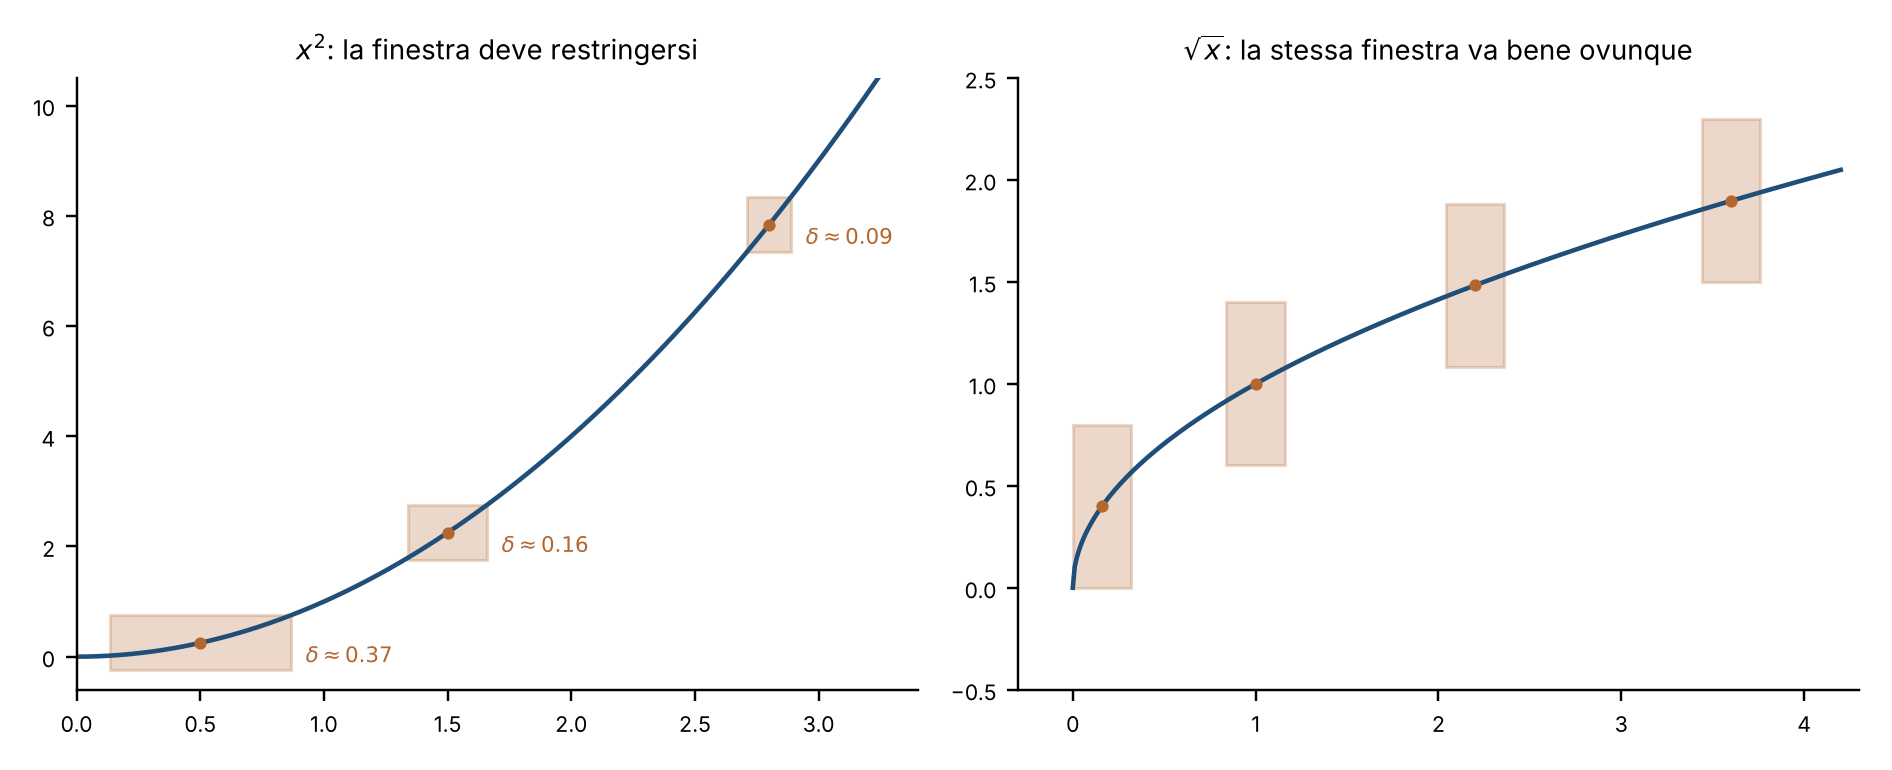
\includegraphics[width=\textwidth]{figure/uniforme.png}
\caption{A sinistra, $f(x)=x^{2}$ con $\epsilon=0{,}5$: per mantenere le variazioni di
$f$ entro $\pm\epsilon$, la finestra deve restringersi man mano che il grafico diventa
più ripido, e la sua semiampiezza è la \eqref{eq:delta-x2}. A destra,
$f(x)=\sqrt x$ con $\epsilon=0{,}4$: la stessa finestra, di semiampiezza
$\delta=\epsilon^{2}=0{,}16$, va bene ovunque, anche vicino all'origine dove la tangente è
verticale (\texttt{python/fig\_uniforme.py}).}
\label{fig:uniforme}
\end{figure}

È opportuno introdurre la definizione seguente.

\begin{definizione}[Funzione uniformemente continua]\label{def:uniformemente-continua}
\index{funzione!uniformemente continua}\index{uniforme continuità}
Si dice che $f:I\to\R$ è \emph{uniformemente continua} nell'intervallo $I$ se per ogni
$\epsilon>0$ esiste $\delta=\delta(\epsilon)>0$ tale che, per ogni $x,x'\in I$,
\begin{equation}\label{eq:uniforme-continuita}
  \abs{x-x'}<\delta \ \implica\ \abs{f(x)-f(x')}<\epsilon .
\end{equation}
\end{definizione}

La differenza con la continuità sta tutta nell'\emph{ordine dei quantificatori}.
Indicata con (C) la condizione
$\abs{x-x_{0}}<\delta\implica\abs{f(x)-f(x_{0})}<\epsilon$, si ha
\[
  \begin{aligned}
    &\text{continuità in } I: &&\perogni x_{0}\in I\ \ \perogni\epsilon>0\ \
    \esiste\delta>0\ \ \perogni x\in I : \ \text{(C)};\\
    &\text{uniforme continuità}: &&\perogni\epsilon>0\ \ \esiste\delta>0\ \
    \perogni x_{0}\in I\ \ \perogni x\in I : \ \text{(C)} .
  \end{aligned}
\]
Nella seconda riga $\delta$ viene scelto \emph{prima} del punto, e deve quindi andar bene
per tutti i punti. Una funzione uniformemente continua è ovviamente continua; il
viceversa è falso, come mostra l'\cref{es:x2-non-uniforme}. Geometricamente, $f$ è
uniformemente continua se un rettangolo di dimensioni fisse $2\delta\times2\epsilon$, fatto
scorrere con il centro sul grafico, è sempre attraversato dal grafico soltanto attraverso
i lati verticali (\cref{fig:uniforme}).

\begin{python}[Il $\delta$ massimo per $x^{2}$ e per $\sqrt x$]
import math

eps = 0.1
print("f(x) = x^2: delta massimo in x0, eps = 0.1")
for x0 in (0, 1, 10, 100, 1000):
    d = math.sqrt(x0**2 + eps) - x0            # formula (delta-x2)
    print(f"   x0 = {x0:7.2f}:  delta = {d:.3e}")
print("f(x) = sqrt(x): delta massimo in x0, eps = 0.1")
for x0 in (0, 0.0025, 1, 100, 1000):
    r = math.sqrt(x0)
    # a destra: (r + eps)^2 - x0;  a sinistra: x0 - (r - eps)^2
    d = 2 * eps * r + eps**2 if r < eps else 2 * eps * r - eps**2
    print(f"   x0 = {x0:7.4g}:  delta = {d:.3e}")
\end{python}
\begin{risultato}
f(x) = x^2: delta massimo in x0, eps = 0.1
   x0 =    0.00:  delta = 3.162e-01
   x0 =    1.00:  delta = 4.881e-02
   x0 =   10.00:  delta = 4.999e-03
   x0 =  100.00:  delta = 5.000e-04
   x0 = 1000.00:  delta = 5.000e-05
f(x) = sqrt(x): delta massimo in x0, eps = 0.1
   x0 =       0:  delta = 1.000e-02
   x0 =  0.0025:  delta = 2.000e-02
   x0 =       1:  delta = 1.900e-01
   x0 =     100:  delta = 1.990e+00
   x0 =    1000:  delta = 6.315e+00
\end{risultato}

Per $x^{2}$ il $\delta$ massimo decresce come $\frac\epsilon{2x_{0}}$; per $\sqrt x$, al
contrario, il più piccolo dei $\delta$ massimi è $\epsilon^{2}>0$ (lo si ha, ad esempio,
nell'origine):
come vedremo nell'\cref{es:radice-uniforme}, la radice quadrata è uniformemente continua
su tutta la semiretta $[0,+\infty)$.

\subsection{Il teorema di Cantor}

Riprendendo l'esempio di $x^{2}$: la funzione non è uniformemente continua su $\R$, ma lo
è in ogni intervallo chiuso e limitato $[a,b]$, grazie al teorema seguente.

\begin{teorema}[di Cantor]\label{teo:cantor}\index{teorema!di Cantor}
Sia $f$ una funzione continua nell'intervallo chiuso e limitato $[a,b]$. Allora $f$ è
uniformemente continua in $[a,b]$.
\end{teorema}

\begin{schema}
\Ipotesi{$f$ continua in $[a,b]$ (chiuso e limitato).}
\Tesi{$\perogni\epsilon>0\ \esiste\delta>0$ : $x,x'\in[a,b]$, $\abs{x-x'}<\delta\implica
\abs{f(x)-f(x')}<\epsilon$.}
\end{schema}

\begin{strategia}
Procediamo per assurdo. Se $f$ non è uniformemente continua, per un certo $\epsilon_{0}$
nessun $\delta$ funziona: scegliendo $\delta=\frac1n$ troviamo coppie di punti
$x_{n}$, $x_{n}'$ sempre più vicine, sulle quali però $f$ differisce di almeno
$\epsilon_{0}$. Qui entra in gioco l'ipotesi che l'intervallo sia chiuso e limitato:
per il teorema di Bolzano--Weierstrass i punti $x_{n}$ hanno un'estratta convergente a
un punto $x_{0}$ di $[a,b]$, e le $x_{n}'$ corrispondenti, vicinissime alle $x_{n}$,
convergono allo stesso punto. La continuità di $f$ in $x_{0}$ costringe allora
$f(x_{n})-f(x_{n}')$ a tendere a zero, in contraddizione con la scelta delle coppie.
\end{strategia}

\begin{dimostrazione}
Procediamo per assurdo. La definizione di uniforme continuità in $[a,b]$ si scrive
\[
  \perogni\epsilon>0\ \ \esiste\delta>0\ \ \perogni x,x'\in[a,b] : \
  \abs{x-x'}<\delta\implica\abs{f(x)-f(x')}<\epsilon ;
\]
la sua negazione afferma che esiste $\epsilon_{0}>0$ tale che, qualunque sia $\delta>0$,
esistono $x,x'\in[a,b]$ (dipendenti da $\delta$) con
\begin{equation}\label{eq:negazione-uc}
  \abs{x-x'}<\delta, \qquad \abs{f(x)-f(x')}\ge\epsilon_{0} .
\end{equation}
Scegliamo $\delta=\frac1n$, con $n\in\N$, e indichiamo con $x_{n}$, $x_{n}'$ i
corrispondenti punti di $[a,b]$ per cui vale la \eqref{eq:negazione-uc}:
\[
  \abs{x_{n}-x_{n}'}<\frac1n, \qquad \abs{f(x_{n})-f(x_{n}')}\ge\epsilon_{0}
  \qquad\perogni n\in\N .
\]
La successione $x_{n}$ è limitata, perché $a\le x_{n}\le b$; per il teorema di
Bolzano--Weierstrass (\cref{teo:bolzano-weierstrass}) esiste un'estratta $x_{n_{k}}$
convergente a un punto $x_{0}$; poiché $a\le x_{n_{k}}\le b$ per ogni $k$, per il
confronto dei limiti (\cref{cor:confronto-limiti}) anche $a\le x_{0}\le b$. È qui che
serve la \emph{chiusura} dell'intervallo. Inoltre
\[
  x_{n_{k}}-\frac1{n_{k}}<x_{n_{k}}'<x_{n_{k}}+\frac1{n_{k}} \qquad\perogni k\in\N,
\]
e poiché $n_{k}\ge k$ (\cref{lem:nk-maggiore-k}) si ha $\frac1{n_{k}}\to0$: per il teorema
dei carabinieri anche $x_{n_{k}}'\to x_{0}$. Le successioni $x_{n_{k}}$ e $x_{n_{k}}'$
sono formate da punti di $[a,b]$ e convergono a $x_{0}\in[a,b]$; per la continuità di
$f$ in $x_{0}$, nella forma (b) della \cref{prop:caratt-continuita},
\[
  \lim_{k\to+\infty}\bigl[f(x_{n_{k}})-f(x_{n_{k}}')\bigr]=f(x_{0})-f(x_{0})=0 ,
\]
in contrasto con il fatto che $\abs{f(x_{n_{k}})-f(x_{n_{k}}')}\ge\epsilon_{0}$ per ogni
$k$. La contraddizione prova la tesi.
\end{dimostrazione}

Entrambe le ipotesi sull'intervallo sono necessarie. Sulla semiretta $[0,+\infty)$,
che è chiusa ma non limitata, $x^{2}$ è continua ma non uniformemente continua
(\cref{es:x2-non-uniforme}); nell'intervallo $(0,1]$, che è limitato ma non chiuso, la
funzione $\frac1x$ è continua ma non uniformemente continua
(\cref{es:uno-su-x-non-uniforme}). In entrambi i casi la dimostrazione si inceppa nello
stesso punto: nel primo la successione $x_{n}$ può non essere limitata, e allora
un'estratta convergente può mancare; nel secondo l'estratta può convergere al punto
$0$, che non appartiene al dominio.

\subsection{Funzioni lipschitziane}

A conclusione del paragrafo riprendiamo una notevole classe di funzioni uniformemente
continue, già incontrata nel \cref{cap:applicazioni-derivate}.

\begin{definizione}[Funzione lipschitziana]\label{def:lipschitziana}
\index{funzione!lipschitziana}
Si dice che $f$ è \emph{lipschitziana} nell'intervallo $I$ se esiste una costante
$L\ge0$, detta \emph{costante di Lipschitz}, tale che
\begin{equation}\label{eq:lipschitziana}
  \abs{f(x)-f(x')}\le L\,\abs{x-x'} \qquad\perogni x,x'\in I .
\end{equation}
\end{definizione}

Per $x\neq x'$ la \eqref{eq:lipschitziana} afferma che le pendenze di tutte le
secanti al grafico sono comprese tra $-L$ e $L$: in ogni punto $(x',f(x'))$ il grafico è
contenuto nel «doppio cono» delimitato dalle rette di pendenza $\pm L$ passanti per quel
punto (\cref{fig:lipschitz}).

\begin{proposizione}[Le lipschitziane sono uniformemente continue]
\label{prop:lipschitz-uniforme}
Una funzione lipschitziana in un intervallo $I$ è uniformemente continua in $I$.
\end{proposizione}

\begin{schema}
\Ipotesi{$\abs{f(x)-f(x')}\le L\abs{x-x'}$ per ogni $x,x'\in I$.}
\Tesi{$f$ uniformemente continua in $I$.}
\end{schema}

\begin{strategia}
La \eqref{eq:lipschitziana} fornisce un $\delta$ esplicito, uguale per tutti i punti:
basta $\delta=\frac\epsilon L$.
\end{strategia}

\begin{dimostrazione}
Se $L=0$, $f$ è costante e la tesi è ovvia. Se $L>0$, fissato $\epsilon>0$ poniamo
$\delta=\frac\epsilon L$: per ogni coppia $x,x'\in I$ con $\abs{x-x'}<\delta$ si ha
$\abs{f(x)-f(x')}\le L\abs{x-x'}<L\delta=\epsilon$.
\end{dimostrazione}

Per le funzioni derivabili la lipschitzianità si legge sulla derivata.

\begin{teorema}[Funzioni derivabili e lipschitziane]\label{teo:lipschitz-derivata}
Sia $f$ derivabile nell'intervallo $I$. Allora $f$ è lipschitziana in $I$ con costante
$L$ se e solo se $\abs{f'(x)}\le L$ per ogni $x\in I$.
\end{teorema}

\begin{schema}
\Ipotesi{$f$ derivabile nell'intervallo $I$; \ $L\ge0$.}
\Tesi{$\abs{f(x)-f(x')}\le L\abs{x-x'}\ \perogni x,x'\in I \ \sse\ \abs{f'}\le L$ in $I$.}
\end{schema}

\begin{strategia}
Una implicazione è il corollario del teorema di Lagrange già dimostrato nel
\cref{cap:applicazioni-derivate}. Per l'altra, la \eqref{eq:lipschitziana} dice che i
rapporti incrementali sono in valore assoluto al più $L$, e il confronto dei limiti
trasmette la stima alla derivata.
\end{strategia}

\begin{dimostrazione}
Se $\abs{f'(x)}\le L$ per ogni $x\in I$, la \eqref{eq:lipschitziana} è la tesi del
\cref{cor:lipschitz}, conseguenza del teorema di Lagrange. Viceversa, sia $f$
lipschitziana con costante $L$ e sia $x\in I$. Per $h\neq0$ con $x+h\in I$ si ha
\[
  \biggl|\frac{f(x+h)-f(x)}h\biggr|\le L .
\]
Per $h\to0$ il rapporto incrementale tende a $f'(x)$, e il suo valore assoluto a
$\abs{f'(x)}$ (per la continuità del valore assoluto); per il confronto dei limiti
(\cref{teo:confronto-funzioni}(ii)) si ottiene $\abs{f'(x)}\le L$.
\end{dimostrazione}

\begin{esempio}[Tre funzioni a confronto]\label{es:lipschitz-esempi}
Tre esempi mostrano i legami tra derivabilità, lipschitzianità e uniforme continuità.
\begin{enumerate}[label=\textup{(\alph*)}]
  \item $\sen x$ è lipschitziana in $\R$ con costante $1$, perché
  $\abs{D\sen x}=\abs{\cos x}\le1$ per ogni $x$; la stessa disuguaglianza
  $\abs{\sen x-\sen x'}\le\abs{x-x'}$ era stata ottenuta nell'\cref{es:seno-lipschitz}
  con le formule di prostaferesi e la disuguaglianza $\abs{\sen t}\le\abs t$.
  \item $\abs x$ è lipschitziana in $\R$ con costante $1$, per la disuguaglianza
  triangolare inversa \eqref{eq:modulo-lipschitz}, ma non è derivabile in $0$: il
  \cref{teo:lipschitz-derivata} non si applica, e una funzione lipschitziana non è
  necessariamente derivabile.
  \item $\sqrt x$ è uniformemente continua in $[0,1]$ per il teorema di Cantor, ma non è
  lipschitziana: la pendenza della secante tra $0$ e $x$ è
  $\frac{\sqrt x-0}{x-0}=\frac1{\sqrt x}$, che tende a $+\infty$ per $x\to0^{+}$, mentre
  dovrebbe essere al più $L$. Equivalentemente, per il \cref{teo:lipschitz-derivata}
  applicato in $(0,1]$, la derivata $\frac1{2\sqrt x}$ non è limitata.
\end{enumerate}
\end{esempio}

\begin{figure}[htb]
\centering
\begin{tikzpicture}
\begin{axis}[name=l1, width=0.55\textwidth, height=4.6cm, axis lines=middle, axis on top,
  xmin=-0.3, xmax=6.5, ymin=-1.9, ymax=2.4, xtick=\empty, ytick=\empty,
  title={\scriptsize $\sen x$: il doppio cono di pendenza $\pm1$}]
  \fill[verde!15] (axis cs:2,0.909) -- (axis cs:6.3,5.209) -- (axis cs:6.3,-3.391)
    -- cycle;
  \fill[verde!15] (axis cs:2,0.909) -- (axis cs:-0.3,3.209) -- (axis cs:-0.3,-1.391)
    -- cycle;
  \addplot[verde!60!black, domain=-0.3:6.3] {0.909+(x-2)};
  \addplot[verde!60!black, domain=-0.3:6.3] {0.909-(x-2)};
  \addplot[curva, domain=-0.3:6.3, samples=120] {sin(deg(x))};
  \addplot[only marks, mark=*, mark size=1.6pt, rame] coordinates {(2,0.909)};
\end{axis}
\begin{axis}[at={(l1.east)}, anchor=west, xshift=0.7cm, width=0.5\textwidth,
  height=4.6cm, axis lines=middle, xmin=-0.05, xmax=1.1, ymin=-0.05, ymax=1.15,
  xtick=\empty, ytick=\empty, title={\scriptsize $\sqrt x$: secanti sempre più ripide}]
  \addplot[curva, domain=0:1.05, samples=200] {sqrt(x)};
  \addplot[rame, domain=0:1.05] {x};
  \addplot[rame, domain=0:0.3] {2*x};
  \addplot[rame, domain=0:0.12] {5*x};
  \addplot[rame, domain=0:0.055] {12*x};
  \addplot[only marks, mark=*, mark size=1.2pt, rame] coordinates
    {(1,1) (0.25,0.5) (0.04,0.2) (0.00694,0.0833)};
  \node[font=\scriptsize, rame, anchor=west] at (axis cs:0.9,0.82) {$1$};
  \node[font=\scriptsize, rame, anchor=west] at (axis cs:0.28,0.62) {$2$};
  \node[font=\scriptsize, rame, anchor=west] at (axis cs:0.11,0.62) {$5$};
  \node[font=\scriptsize, rame, anchor=south] at (axis cs:0.052,0.66) {$12$};
\end{axis}
\end{tikzpicture}
\caption{A sinistra, una funzione lipschitziana con costante $L=1$: il grafico di
$\sen x$ resta nel doppio cono verde, delimitato dalle rette di pendenza $\pm1$ per il
punto evidenziato, e così per ogni altro punto. A destra, le secanti al grafico di
$\sqrt x$ uscenti dall'origine hanno pendenze $1$, $2$, $5$, $12$, \dots, non limitate:
nessun cono di apertura finita contiene il grafico vicino all'origine.}
\label{fig:lipschitz}
\end{figure}

\begin{esempio}[La radice quadrata è uniformemente continua su $\lbrack0,+\infty)$]
\label{es:radice-uniforme}
Il teorema di Cantor non si applica alla semiretta, ma per la radice quadrata vale una
stima diretta: per $0\le x'\le x$,
\begin{equation}\label{eq:radice-holder}
  \sqrt x-\sqrt{x'}\le\sqrt{x-x'} .
\end{equation}
Infatti, elevando al quadrato i due membri non negativi di
$\sqrt x\le\sqrt{x-x'}+\sqrt{x'}$, la disuguaglianza equivale a
$x\le(x-x')+2\sqrt{x'(x-x')}+x'$, cioè a $0\le2\sqrt{x'(x-x')}$, che è vera. Dunque
$\abs{\sqrt x-\sqrt{x'}}\le\sqrt{\abs{x-x'}}$ per ogni $x,x'\ge0$, e posto
$\delta=\epsilon^{2}$ si ha $\abs{\sqrt x-\sqrt{x'}}<\epsilon$ non appena
$\abs{x-x'}<\delta$: la radice è uniformemente continua in $[0,+\infty)$ pur non essendo
lipschitziana. Una stima del tipo $\abs{f(x)-f(x')}\le L\abs{x-x'}^{\alpha}$, con
$0<\alpha\le1$, si chiama \emph{condizione di Hölder}; per $\alpha=1$ è la
lipschitzianità.
\end{esempio}

\begin{python}[Pendenze delle secanti: seno e radice quadrata]
import math, random

random.seed(1)
pend = []
for _ in range(100000):
    x, y = random.uniform(-10, 10), random.uniform(-10, 10)
    if x != y:
        pend.append(abs(math.sin(x) - math.sin(y)) / abs(x - y))
print(f"sen x: pendenza massima delle secanti = {max(pend):.6f}")
for h in (1e-2, 1e-4, 1e-6, 1e-8):
    print(f"sqrt(x): pendenza della secante tra 0 e {h:.0e}"
          f" = {math.sqrt(h) / h:7.0f}")
\end{python}
\begin{risultato}
sen x: pendenza massima delle secanti = 0.999970
sqrt(x): pendenza della secante tra 0 e 1e-02 =      10
sqrt(x): pendenza della secante tra 0 e 1e-04 =     100
sqrt(x): pendenza della secante tra 0 e 1e-06 =    1000
sqrt(x): pendenza della secante tra 0 e 1e-08 =   10000
\end{risultato}

Riassumendo, per una funzione definita in un intervallo valgono le implicazioni
illustrate nella \cref{fig:gerarchia}, nessuna delle quali si può invertire.

\begin{figure}[htb]
\centering
\begin{tikzpicture}[box/.style={draw=blu, fill=blu!8, rounded corners=2pt,
  font=\scriptsize, align=center, inner sep=4pt, minimum height=1.0cm,
  text width=1.95cm}]
  \node[box] (a) at (0,0) {derivabile con\\ $f'$ limitata};
  \node[box] (b) at (2.85,0) {lipschitziana};
  \node[box] (c) at (5.7,0) {uniformemente\\ continua};
  \node[box] (d) at (8.55,0) {continua};
  \draw[-Latex, thick, grigio] (a) -- (b);
  \draw[-Latex, thick, grigio] (b) -- (c);
  \draw[-Latex, thick, grigio] (c) -- (d);
  \node[font=\scriptsize, rame, align=center] at (1.425,-1.0) {$\abs x$ su $\R$};
  \node[font=\scriptsize, rame, align=center] at (4.275,-1.0) {$\sqrt x$ su $[0,1]$};
  \node[font=\scriptsize, rame, align=center] at (7.125,-1.05)
    {$x^{2}$ su $\R$,\\ $\frac1x$ su $(0,1]$};
\end{tikzpicture}
\caption{Le implicazioni tra le classi di funzioni in un intervallo. Sotto ciascuna
freccia, una funzione che appartiene alla classe di destra ma non a quella di sinistra.
Per un intervallo chiuso e limitato, il teorema di Cantor rende equivalenti le ultime
due classi.}
\label{fig:gerarchia}
\end{figure}

\begin{notastorica}[Dirichlet, Heine, Cantor]
Nella dimostrazione dell'integrabilità delle funzioni continue data da Cauchy nel 1823
c'era una lacuna: Cauchy usava senza accorgersene la continuità \emph{uniforme}, non
distinguendola da quella puntuale. La distinzione maturò negli anni successivi.
Peter Gustav Lejeune Dirichlet dimostrò il teorema che abbiamo chiamato di Cantor nelle
sue lezioni berlinesi del 1854 sugli integrali definiti, pubblicate però soltanto nel
1904. Il primo a pubblicare questi risultati fu Eduard Heine: la definizione di
uniforme continuità nel 1870, il teorema nel 1872, in un articolo sui fondamenti della
teoria delle funzioni nel quale riconosceva il proprio debito verso le idee di
Weierstrass e di Georg Cantor; per questo il teorema è noto anche come teorema di
Heine--Cantor. Rudolf Lipschitz considerò per la prima volta una condizione del tipo
\eqref{eq:lipschitziana} nel 1864, studiando la convergenza delle serie di Fourier; nel
1876 la pose come ipotesi che garantisce l'esistenza e l'unicità delle soluzioni delle
equazioni differenziali. È ancora oggi l'ipotesi standard dei teoremi di esistenza e
unicità che si incontrano, ad esempio, nello studio della dinamica del volo.
\end{notastorica}

%% ----------------------------------------------------------------------------
%%  §8.6  Appendice: integrabilità delle funzioni continue e monotòne
%% ----------------------------------------------------------------------------
\section{Appendice: integrabilità delle funzioni continue e monotòne}
\label{sec:integrabilita-continue}

Possiamo ora dimostrare il risultato che rende la teoria dell'integrale utilizzabile in
pratica: tutte le funzioni continue in un intervallo chiuso e limitato sono
integrabili. Lo otterremo in una forma più forte, che riguarda \emph{tutte} le
partizioni di ampiezza sufficientemente piccola, e che giustificherà le formule di
quadratura numerica.

\begin{teorema}[Integrabilità delle funzioni continue]\label{teo:integrabilita-continue}
\index{funzione!continua!integrabilità}
Sia $f$ una funzione continua in $[a,b]$. Allora $f$ è integrabile secondo Riemann in
$[a,b]$. Più precisamente, per ogni $\epsilon>0$ esiste $\delta>0$ tale che
\begin{equation}\label{eq:ampiezza-piccola}
  \abs P<\delta \ \implica\ S(P)-s(P)<\epsilon \qquad\text{per ogni partizione $P$ di }
  [a,b] .
\end{equation}
\end{teorema}

\begin{schema}
\Ipotesi{$f$ continua in $[a,b]$, $a<b$.}
\Tesi{$f$ integrabile in $[a,b]$; \ $\perogni\epsilon>0\ \esiste\delta>0$ :
$\abs P<\delta\implica S(P)-s(P)<\epsilon$.}
\end{schema}

\begin{strategia}
Per la \eqref{eq:S-s-oscillazioni} basta rendere tutte le oscillazioni $M_{k}-m_{k}$
minori di $\frac\epsilon{b-a}$: allora $S(P)-s(P)<\frac\epsilon{b-a}\sum\Delta
x_{k}=\epsilon$. Il teorema di Weierstrass assicura che $m_{k}$ e $M_{k}$ sono valori di
$f$ in due punti dell'intervallo $[x_{k-1},x_{k}]$, la cui distanza non supera
l'ampiezza della partizione; il teorema di Cantor fornisce un $\delta$, \emph{uguale per
tutti gli intervalli}, che rende piccola la differenza tra due valori di $f$ in punti
distanti meno di $\delta$.
\end{strategia}

\begin{dimostrazione}
La funzione $f$ è limitata per il teorema di Weierstrass, quindi le somme integrali
sono definite. Fissato $\epsilon>0$, per il teorema di Cantor (\cref{teo:cantor}) $f$ è
uniformemente continua in $[a,b]$, ed esiste $\delta>0$ tale che
\begin{equation}\label{eq:cantor-integrabilita}
  \abs{f(x)-f(x')}<\frac\epsilon{b-a} \qquad\text{per ogni } x,x'\in[a,b] \text{ con }
  \abs{x-x'}<\delta .
\end{equation}
Sia $P=\set{x_{0},\dots,x_{n}}$ una partizione con $\abs P<\delta$. In ogni intervallo
$[x_{k-1},x_{k}]$ la funzione continua $f$ assume minimo e massimo (\cref{teo:weierstrass}):
esistono $\xi_{k},\eta_{k}\in[x_{k-1},x_{k}]$ con $m_{k}=f(\xi_{k})$ e $M_{k}=f(\eta_{k})$.
Poiché $\abs{\xi_{k}-\eta_{k}}\le\Delta x_{k}\le\abs P<\delta$, per la
\eqref{eq:cantor-integrabilita}
\[
  M_{k}-m_{k}=f(\eta_{k})-f(\xi_{k})<\frac\epsilon{b-a} \qquad\perogni k=1,\dots,n ,
\]
e quindi
\[
  S(P)-s(P)=\sum_{k=1}^{n}(M_{k}-m_{k})\,\Delta x_{k}
  <\frac\epsilon{b-a}\sum_{k=1}^{n}\Delta x_{k}=\epsilon .
\]
Questo prova la \eqref{eq:ampiezza-piccola}. Partizioni di ampiezza minore di $\delta$
esistono (ad esempio la partizione uniforme in $n$ parti, con $n>\frac{b-a}\delta$), e il
criterio di integrabilità (\cref{teo:criterio-integrabilita}) dà l'integrabilità di
$f$.
\end{dimostrazione}

La forma forte \eqref{eq:ampiezza-piccola} ha una conseguenza importante: per una
funzione continua, l'integrale è il limite di \emph{qualsiasi} successione di somme di
Riemann, purché l'ampiezza delle partizioni tenda a zero.

\begin{teorema}[Convergenza delle somme di Riemann]\label{teo:riemann-continue}
Sia $f$ continua in $[a,b]$, sia $P_{n}$ una successione di partizioni di $[a,b]$ con
$\abs{P_{n}}\to0$, e sia $\sigma_{n}$ una somma di Riemann \eqref{eq:somma-riemann}
relativa a $P_{n}$, con punti $\xi_{k}$ scelti in modo arbitrario. Allora
\begin{equation}\label{eq:riemann-limite}
  \lim_{n\to+\infty}\sigma_{n}=\int_{a}^{b}f(x)\,dx .
\end{equation}
\end{teorema}

\begin{schema}
\Ipotesi{$f$ continua in $[a,b]$; \ $\abs{P_{n}}\to0$; \ $\sigma_{n}$ somma di Riemann
relativa a $P_{n}$.}
\Tesi{$\sigma_{n}\to\int_{a}^{b}f$.}
\end{schema}

\begin{strategia}
Ogni somma di Riemann dista dall'integrale al più $S(P)-s(P)$ \eqref{eq:riemann-stima}, e
questa quantità è piccola quando l'ampiezza della partizione è piccola, per la
\eqref{eq:ampiezza-piccola}.
\end{strategia}

\begin{dimostrazione}
Sia $\epsilon>0$ e sia $\delta$ quello del \cref{teo:integrabilita-continue}. Poiché
$\abs{P_{n}}\to0$, esiste $\nu$ tale che $\abs{P_{n}}<\delta$ per ogni $n>\nu$; per tali $n$,
la \eqref{eq:riemann-stima} e la \eqref{eq:ampiezza-piccola} danno
$\bigl|\sigma_{n}-\int_{a}^{b}f\bigr|\le S(P_{n})-s(P_{n})<\epsilon$.
\end{dimostrazione}

In particolare, per $f$ continua le medie aritmetiche di $n$ campioni equispaziati,
come quelle considerate all'inizio del \cref{sec:media}, tendono alla media integrale.

\subsection{Funzioni monotòne}

La continuità è sufficiente ma non necessaria per l'integrabilità: la funzione
dell'\cref{oss:media-discontinua} è discontinua ma integrabile. Un'altra classe
importante di funzioni integrabili, che comprende funzioni discontinue, è quella delle
funzioni monotòne.

\begin{teorema}[Integrabilità delle funzioni monotòne]\label{teo:integrabilita-monotone}
\index{funzione!monotòna!integrabilità}
Sia $f$ monotòna in $[a,b]$. Allora $f$ è integrabile secondo Riemann in $[a,b]$, e per
la partizione uniforme $P_{n}$ in $n$ parti risulta
\begin{equation}\label{eq:monotone-S-s}
  S(P_{n})-s(P_{n})=\frac{\abs{f(b)-f(a)}\,(b-a)}n .
\end{equation}
\end{teorema}

\begin{schema}
\Ipotesi{$f$ monotòna in $[a,b]$.}
\Tesi{$f$ integrabile; \ $S(P_{n})-s(P_{n})=\abs{f(b)-f(a)}\frac{b-a}n$.}
\end{schema}

\begin{strategia}
È il calcolo già fatto per $x^{2}$, per la distribuzione ellittica e per
$e^{-x^{2}}$: in ogni intervallo gli estremi di una funzione monotòna sono i valori negli
estremi dell'intervallo, e la differenza tra le somme è telescopica.
\end{strategia}

\begin{dimostrazione}
Una funzione monotòna in $[a,b]$ è limitata, perché i suoi valori sono compresi tra
$f(a)$ e $f(b)$. Sia $f$ crescente e sia $x_{k}=a+k\frac{b-a}n$. Per
$x\in[x_{k-1},x_{k}]$ si ha $f(x_{k-1})\le f(x)\le f(x_{k})$, e i valori $f(x_{k-1})$,
$f(x_{k})$ sono assunti; quindi $m_{k}=f(x_{k-1})$ e $M_{k}=f(x_{k})$, e
\[
  S(P_{n})-s(P_{n})=\frac{b-a}n\sum_{k=1}^{n}\bigl[f(x_{k})-f(x_{k-1})\bigr]
  =\frac{b-a}n\bigl[f(b)-f(a)\bigr] .
\]
Se $f$ è decrescente, si scambiano i ruoli di $x_{k-1}$ e $x_{k}$ e si ottiene
$\frac{b-a}n\bigl[f(a)-f(b)\bigr]$. In entrambi i casi vale la \eqref{eq:monotone-S-s}, che
tende a zero, e il \cref{cor:limite-somme} dà l'integrabilità.
\end{dimostrazione}

Una funzione monotòna può avere infiniti punti di discontinuità (che sono salti, per il
\cref{cor:monotone-salti}). Ad esempio, la funzione definita in $[0,1]$ da $f(0)=0$ e
$f(x)=\frac1n$ per $\frac1{n+1}<x\le\frac1n$, $n\in\N$, è crescente, ha un salto in ciascuno
dei punti $\frac1n$ con $n\ge2$, ed è integrabile per il \cref{teo:integrabilita-monotone}.

\subsection{Formule di quadratura}

Il \cref{teo:riemann-continue} giustifica il calcolo numerico degli integrali delle
funzioni continue mediante somme di Riemann. Con la partizione uniforme di passo
$h=\frac{b-a}n$ e nodi $x_{k}=a+kh$, le formule più semplici sono quella dei
\emph{rettangoli} (con l'estremo sinistro), quella del \emph{punto medio} e quella dei
\emph{trapezi}:
\begin{align}
  R_{n}&=h\sum_{k=0}^{n-1}f(x_{k}),
  \label{eq:quadratura-rettangoli}\\
  M_{n}&=h\sum_{k=1}^{n}f\Bigl(\frac{x_{k-1}+x_{k}}2\Bigr),
  \label{eq:quadratura-medio}\\
  T_{n}&=h\Bigl[\frac{f(x_{0})+f(x_{n})}2+\sum_{k=1}^{n-1}f(x_{k})\Bigr].
  \label{eq:quadratura-trapezi}
\end{align}
Le prime due sono somme di Riemann, e convergono all'integrale per il
\cref{teo:riemann-continue}. La terza è la media aritmetica della somma dei rettangoli
con l'estremo sinistro e di quella con l'estremo destro, e converge per lo stesso
motivo; il nome deriva dal fatto che, per $f\ge0$, $T_{n}$ è la somma delle aree dei
trapezi di altezza $h$ e basi $f(x_{k-1})$, $f(x_{k})$ (\cref{fig:quadratura}).

Le tre formule non convergono però con la stessa rapidità. Per una funzione monotòna
l'errore della formula dei rettangoli non supera la \eqref{eq:monotone-S-s}, che è
dell'ordine di $\frac1n$, e in generale non è più piccolo. Per il punto medio e per i
trapezi, invece, si dimostra con la formula di Taylor (lo si fa nei corsi di Calcolo
numerico) che, se $f$ ha derivata seconda continua,
\begin{equation}\label{eq:errori-quadratura}
\begin{aligned}
  \Bigl|M_{n}-\int_{a}^{b}f\Bigr|&\le\frac{(b-a)\,h^{2}}{24}\max_{[a,b]}\abs{f''},\\
  \Bigl|T_{n}-\int_{a}^{b}f\Bigr|&\le\frac{(b-a)\,h^{2}}{12}\max_{[a,b]}\abs{f''} :
\end{aligned}
\end{equation}
raddoppiando $n$ l'errore si riduce di circa quattro volte. Inoltre l'errore del punto
medio è circa la metà di quello dei trapezi e di segno opposto, per cui la combinazione
$\frac{2M_{n}+T_{n}}3$, che è la \emph{formula di Cavalieri--Simpson}, elimina il termine
principale dell'errore. Il programma seguente lo verifica sull'integrale
$\int_{0}^{1}e^{-x^{2}}dx$ dell'\cref{es:stima-gaussiana}.

\begin{python}[Formule di quadratura a confronto]
import math

f = lambda x: math.exp(-x * x)
I = math.erf(1) * math.sqrt(math.pi) / 2     # valore di riferimento

def quadrature(f, a, b, n):
    """Rettangoli, punto medio, trapezi, Cavalieri-Simpson."""
    h = (b - a) / n
    x = [a + k * h for k in range(n + 1)]
    ret = h * sum(f(x[k]) for k in range(n))
    med = h * sum(f(x[k] + h / 2) for k in range(n))
    tra = h * (sum(f(t) for t in x) - (f(a) + f(b)) / 2)
    return ret, med, tra, (2 * med + tra) / 3

print("errori assoluti")
print(f"{'n':>4} {'rettangoli':>11} {'p. medio':>10}"
      f" {'trapezi':>10} {'Simpson':>10}")
for n in (4, 8, 16, 32, 64):
    err = [abs(q - I) for q in quadrature(f, 0, 1, n)]
    print(f"{n:4d} " + " ".join(f"{e:10.2e}" for e in err))
\end{python}
\begin{risultato}
errori assoluti
   n  rettangoli   p. medio    trapezi    Simpson
   4   7.52e-02   1.92e-03   3.84e-03   1.99e-06
   8   3.85e-02   4.79e-04   9.59e-04   1.25e-07
  16   1.95e-02   1.20e-04   2.40e-04   7.79e-09
  32   9.82e-03   2.99e-05   5.99e-05   4.87e-10
  64   4.92e-03   7.48e-06   1.50e-05   3.05e-11
\end{risultato}

\begin{figure}[htb]
\centering
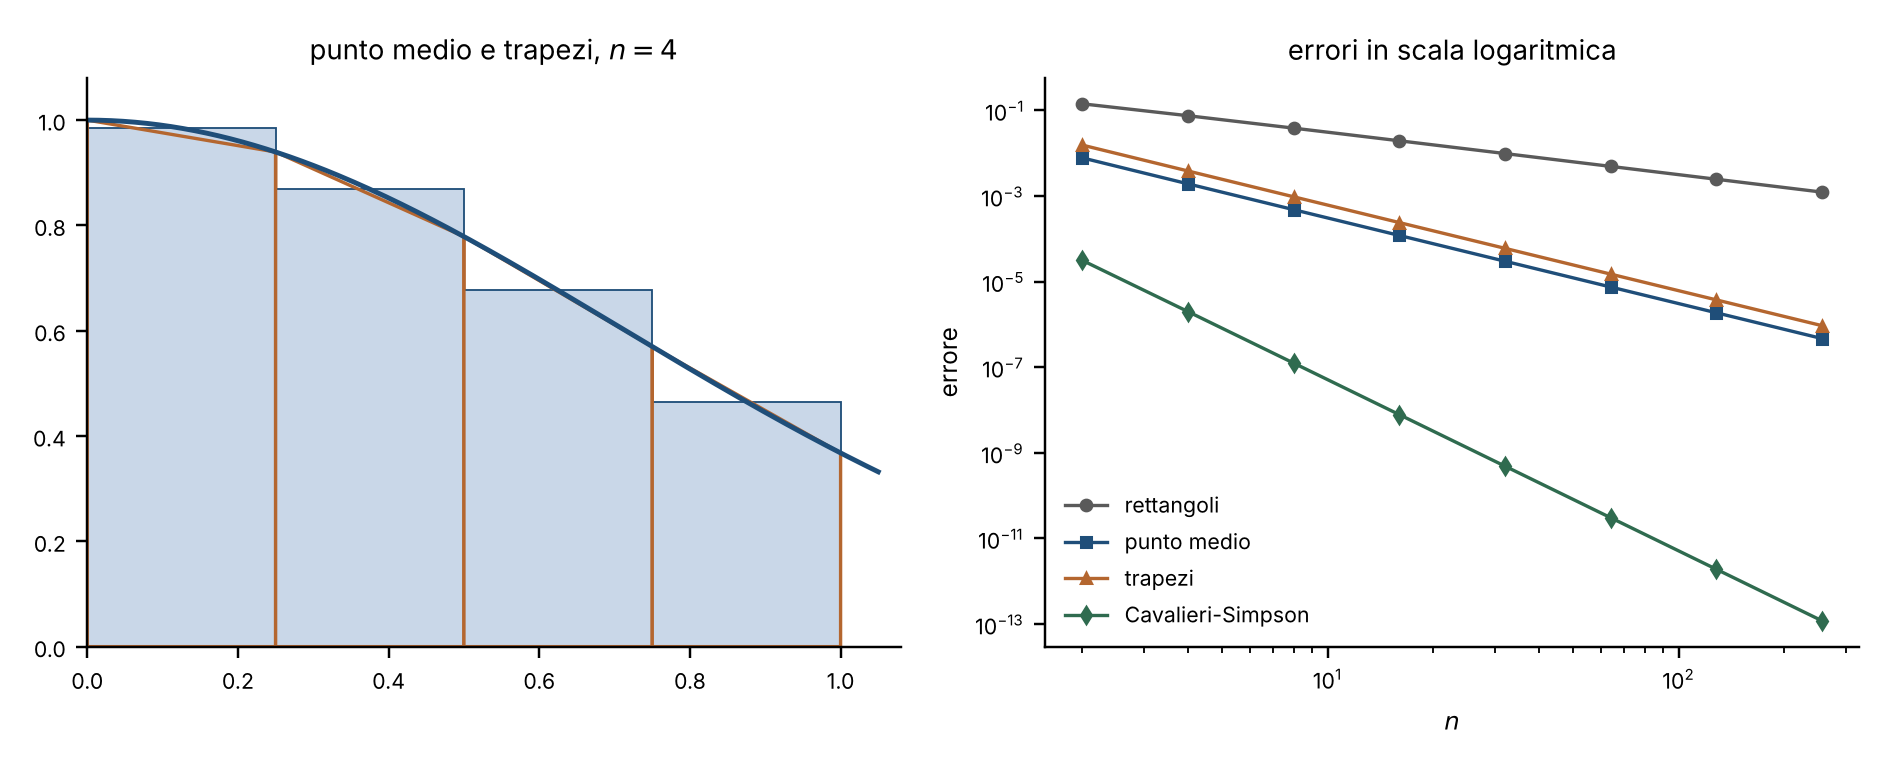
\includegraphics[width=\textwidth]{figure/quadratura.png}
\caption{A sinistra, le formule del punto medio (rettangoli azzurri) e dei trapezi
(contorni in color rame) per $e^{-x^{2}}$ in $[0,1]$ con $n=4$. A destra, gli errori
delle quattro formule in funzione di $n$, in scala logaritmica: le pendenze $-1$, $-2$
e $-4$ corrispondono a errori proporzionali a $\frac1n$, $\frac1{n^{2}}$, $\frac1{n^{4}}$
(\texttt{python/fig\_quadratura.py}).}
\label{fig:quadratura}
\end{figure}

\begin{notastorica}[Da Cauchy a Lebesgue]
Cauchy dimostrò nel 1823 che le somme costruite sugli estremi sinistri di una funzione
continua convergono, quando l'ampiezza della partizione tende a zero, a un limite
indipendente dalle partizioni: è un caso particolare del nostro
\cref{teo:riemann-continue} (sulla lacuna della dimostrazione si veda la nota del
\S\ref{sec:uniforme-continuita}). Riemann, con il suo criterio, estese l'integrale a
funzioni con infinite discontinuità: quali funzioni limitate sono integrabili?
Dirichlet, nella memoria del 1829 in cui compare la sua funzione (\cref{oss:dirichlet}),
aveva indicato come necessario che tra due punti qualsiasi si trovasse sempre un
intervallo di continuità; ma Riemann costruì una funzione integrabile discontinua in un
insieme denso. Hermann Hankel (1870) credette che un insieme non denso in alcun
intervallo si potesse racchiudere in un numero finito di intervalli di lunghezza totale
piccola a piacere; Henry Smith (1875) mostrò che non è così. La risposta
definitiva venne all'inizio del Novecento da Henri Lebesgue e, indipendentemente, da
Giuseppe Vitali (1903): sono integrabili le funzioni limitate il cui insieme dei punti di
discontinuità ha \emph{misura nulla}, cioè si può ricoprire con una successione di
intervalli di lunghezza totale piccola a piacere (come l'insieme numerabile dei salti di
una funzione monotòna, ma non $[0,1]$, dove è discontinua la funzione di Dirichlet).
Quanto alle formule di quadratura, quella che in Italia porta il nome di
Cavalieri--Simpson era nota, in forme equivalenti, a Keplero, che nel 1615 la usò per
stimare il volume delle botti, a Bonaventura Cavalieri e a James Gregory, prima che
Thomas Simpson la diffondesse nel 1743.
\end{notastorica}

%% ----------------------------------------------------------------------------
%%  §8.7  Esercizi di riepilogo
%% ----------------------------------------------------------------------------
\section{Esercizi di riepilogo}
\label{sec:esercizi-cap8}

Come nei capitoli precedenti, ogni soluzione è accompagnata da una nota sulla
\emph{scelta logica} che la guida.

\needspace{8\baselineskip}
\subsection*{Somme integrali e definizione}

\begin{esercizio}\label{es:integrale-x3}
Dimostrare per induzione che $\sum_{k=1}^{n}k^{3}=\bigl(\frac{n(n+1)}2\bigr)^{2}$ e dedurne
che $\int_{0}^{b}x^{3}\,dx=\frac{b^{4}}4$ per ogni $b>0$.
\begin{soluzione}
Per $n=1$ entrambi i membri valgono $1$. Se la formula vale per $n$, allora
$\sum_{k=1}^{n+1}k^{3}=\frac{n^{2}(n+1)^{2}}4+(n+1)^{3}=\frac{(n+1)^{2}}4\bigl(n^{2}+4n+4\bigr)
=\frac{(n+1)^{2}(n+2)^{2}}4$, che è la formula per $n+1$. Per la partizione uniforme di
$[0,b]$ e la funzione crescente $x^{3}$, $M_{k}=x_{k}^{3}$ e $m_{k}=x_{k-1}^{3}$:
\[
  S(P_{n})=\frac bn\sum_{k=1}^{n}\frac{k^{3}b^{3}}{n^{3}}=\frac{b^{4}}4\cdot\frac{(n+1)^{2}}{n^{2}},
  \qquad
  s(P_{n})=\frac{b^{4}}4\cdot\frac{(n-1)^{2}}{n^{2}} ,
\]
con $S(P_{n})-s(P_{n})=\frac{b^{4}}n\to0$ (somma telescopica, come nella
\eqref{eq:monotone-S-s}). Per il \cref{cor:limite-somme} l'integrale è il limite comune,
$\frac{b^{4}}4$. \emph{Scelta logica:} lo schema è quello del settore di parabola; i
risultati $\frac{b^{2}}2$, $\frac{b^{3}}3$, $\frac{b^{4}}4$ suggeriscono
$\int_{0}^{b}x^{p}\,dx=\frac{b^{p+1}}{p+1}$, e la derivata rispetto a $b$ di ciascuno è
$b^{p}$: è ancora l'indizio dell'\cref{oss:indizio-tfc}.
\end{soluzione}
\end{esercizio}

\begin{esercizio}\label{es:integrale-esponenziale}
Calcolare $\int_{0}^{1}2^{x}\,dx$ con le somme integrali relative alla partizione
uniforme.
\begin{soluzione}
La funzione è crescente, quindi $M_{k}=2^{k/n}$. Posto $q=2^{1/n}$, la somma superiore è
una progressione geometrica (\cref{prop:geometrica}):
\[
  S(P_{n})=\frac1n\sum_{k=1}^{n}q^{k}=\frac1n\cdot\frac{q\,(q^{n}-1)}{q-1}
  =2^{1/n}\cdot\frac{1/n}{2^{1/n}-1},
\]
perché $q^{n}=2$. Per il limite notevole \eqref{eq:ln-exp}, calcolato lungo la
successione $\frac1n\to0$, $\frac{2^{1/n}-1}{1/n}\to\log2$; inoltre $2^{1/n}\to1$. Dunque
$S(P_{n})\to\frac1{\log2}$. Per il \cref{teo:integrabilita-monotone},
$S(P_{n})-s(P_{n})=\frac1n(2-1)\to0$, e quindi anche $s(P_{n})\to\frac1{\log2}$: per il
\cref{cor:limite-somme}
$\int_{0}^{1}2^{x}\,dx=\frac1{\log2}\approx1{,}4427$. \emph{Scelta logica:} per gli
esponenziali la partizione uniforme trasforma la somma in una progressione geometrica
(nel procedimento di Fermat la progressione geometrica compariva invece nei nodi della
partizione); il calcolo si chiude con un limite notevole del
\cref{cap:funzioni-continue}.
\end{soluzione}
\end{esercizio}

\begin{esercizio}\label{es:integrale-a-b}
Dimostrare che, per $0\le a<b$, $\int_{a}^{b}x\,dx=\frac{b^{2}-a^{2}}2$ e
$\int_{a}^{b}x^{2}\,dx=\frac{b^{3}-a^{3}}3$, e calcolare la media integrale di $x^{2}$ in
$[a,b]$.
\begin{soluzione}
Per l'additività (\cref{teo:additivita}), $\int_{0}^{b}=\int_{0}^{a}+\int_{a}^{b}$, quindi
$\int_{a}^{b}x^{2}\,dx=\frac{b^{3}}3-\frac{a^{3}}3$ per la \eqref{eq:integrale-x2}, e
analogamente per $x$. La media è
$\frac{b^{3}-a^{3}}{3(b-a)}=\frac{a^{2}+ab+b^{2}}3$. \emph{Scelta logica:} l'additività
permette di ottenere l'integrale su un intervallo qualsiasi da quelli con primo estremo
nell'origine, senza nuove somme.
\end{soluzione}
\end{esercizio}

\begin{esercizio}\label{es:valore-in-un-punto}
Sia $f$ integrabile in $[a,b]$ e sia $g$ una funzione che differisce da $f$ in un solo
punto $\bar x$. Dimostrare che $g$ è integrabile e che $\int_{a}^{b}g=\int_{a}^{b}f$.
\begin{soluzione}
La funzione $h=g-f$ è nulla tranne che in $\bar x$, dove vale $d\neq0$; supponiamo
$d>0$ (altrimenti si ragiona su $-h$). In ogni intervallo di una partizione $P$ esistono
punti diversi da $\bar x$, quindi $m_{k}=0$ e $s(P,h)=0$; inoltre $M_{k}=d$ negli intervalli
(al più due) che contengono $\bar x$, e $M_{k}=0$ negli altri, quindi
$0\le S(P,h)\le2d\abs P$. Per la partizione uniforme $P_{n}$, $S(P_{n},h)-s(P_{n},h)\to0$, e
per il \cref{cor:limite-somme} $h$ è integrabile con integrale $0$. Per la linearità,
$g=f+h$ è integrabile e $\int g=\int f+0$. Ripetendo il ragionamento, la conclusione vale
anche se $g$ differisce da $f$ in un numero finito di punti. \emph{Scelta logica:} un
punto «non ha larghezza», e i rettangoli che lo contengono hanno area totale piccola
quanto l'ampiezza della partizione. Modificando $f$ in \emph{infiniti} punti, invece,
l'integrabilità si può perdere: la funzione di Dirichlet si ottiene dalla funzione
nulla cambiandone il valore nei razionali.
\end{soluzione}
\end{esercizio}

\begin{esercizio}
Sia $f(x)=x$ per $x\in\Q$ e $f(x)=0$ per $x\notin\Q$. Calcolare l'integrale inferiore e
l'integrale superiore di $f$ in $[0,1]$.
\begin{soluzione}
In ogni intervallo $[x_{k-1},x_{k}]$ ci sono irrazionali, dove $f=0$, e razionali
arbitrariamente vicini a $x_{k}$, per la densità di $\Q$; poiché
$0\le f(x)\le x\le x_{k}$ in $[x_{k-1},x_{k}]$, risulta $m_{k}=0$ e $M_{k}=x_{k}$. Dunque $s(P,f)=0$ per ogni $P$, e $s(f)=0$; e
$S(P,f)=\sum x_{k}\Delta x_{k}=S(P,\mathrm{id})$ è la somma superiore della funzione
$\mathrm{id}(x)=x$, quindi $S(f)=\inf_{P}S(P,\mathrm{id})=\int_{0}^{1}x\,dx=\frac12$. Poiché
$0\neq\frac12$, $f$ non è integrabile. \emph{Scelta logica:} le somme di $f$ si
riconducono a quelle di funzioni note (la funzione nulla e l'identità); l'esempio
mostra che $s(f)$ e $S(f)$ possono essere entrambi calcolabili e diversi.
\end{soluzione}
\end{esercizio}

\needspace{8\baselineskip}
\subsection*{Proprietà, simmetrie, stime}

\begin{esercizio}\label{es:riflessione}
Sia $f$ integrabile in $[-a,a]$, con $a>0$. Dimostrare che
$\int_{-a}^{0}f(x)\,dx=\int_{0}^{a}f(-t)\,dt$, e dedurne che
$\int_{-a}^{a}f=0$ se $f$ è dispari e $\int_{-a}^{a}f=2\int_{0}^{a}f$ se $f$ è pari.
\begin{soluzione}
Sia $g(t)=f(-t)$ per $t\in[0,a]$. A ogni partizione $P=\set{x_{0},\dots,x_{n}}$ di
$[0,a]$ corrisponde la partizione $-P=\set{-x_{n},\dots,-x_{0}}$ di $[-a,0]$, e la
corrispondenza è biunivoca. I valori di $g$ in $[x_{k-1},x_{k}]$ sono i valori di $f$ in
$[-x_{k},-x_{k-1}]$, intervallo della stessa ampiezza: quindi $s(P,g)=s(-P,f)$ e
$S(P,g)=S(-P,f)$. Gli insiemi delle somme inferiori e superiori di $g$ in $[0,a]$
coincidono con quelli di $f$ in $[-a,0]$, e così gli integrali. Se $f$ è dispari,
$f(-t)=-f(t)$, e per l'additività e la linearità
$\int_{-a}^{a}f=\int_{0}^{a}f(-t)\,dt+\int_{0}^{a}f=-\int_{0}^{a}f+\int_{0}^{a}f=0$; se $f$ è pari
si ottiene $2\int_{0}^{a}f$. \emph{Scelta logica:} una trasformazione che manda partizioni
in partizioni conservando le ampiezze, e valori in valori, conserva le somme integrali
e quindi l'integrale. Ritroviamo così il valore $0$ trovato numericamente per
$x^{3}-3x$ in $[-2,2]$, e la simmetria delle due semiali nell'\cref{es:corda-media}.
\end{soluzione}
\end{esercizio}

\begin{esercizio}\label{es:scala-traslazione}
Sia $f$ integrabile in $[a,b]$. Dimostrare che, per ogni $\alpha>0$ e ogni $c\in\R$,
\[
  \int_{\alpha a}^{\alpha b}f\Bigl(\frac x\alpha\Bigr)dx=\alpha\int_{a}^{b}f(t)\,dt, \qquad
  \int_{a+c}^{b+c}f(x-c)\,dx=\int_{a}^{b}f(t)\,dt .
\]
\begin{soluzione}
Si ragiona come nell'esercizio precedente. La corrispondenza $P\mapsto\alpha P$ è
biunivoca tra le partizioni di $[a,b]$ e quelle di $[\alpha a,\alpha b]$; la funzione
$x\mapsto f(x/\alpha)$ assume nell'intervallo $[\alpha x_{k-1},\alpha x_{k}]$ gli stessi
valori che $f$ assume in $[x_{k-1},x_{k}]$, mentre le ampiezze si moltiplicano per
$\alpha$. Quindi tutte le somme inferiori e superiori si moltiplicano per $\alpha$, e
così l'integrale. Per la traslazione le ampiezze non cambiano. \emph{Scelta logica:}
sono i primi, semplicissimi casi della \emph{formula di cambiamento di variabile} che
studieremo nel prossimo capitolo.
\end{soluzione}
\end{esercizio}

\begin{esercizio}\label{es:portanza-ellittica-esatta}
Calcolare la portanza totale $L=\int_{-b/2}^{b/2}l(y)\,dy$ per la distribuzione
ellittica \eqref{eq:portanza-ellittica}.
\begin{soluzione}
La funzione $l$ è continua, quindi integrabile. Con la formula di cambiamento di scala
dell'esercizio precedente, con $\alpha=\frac b2$,
\[
  L=l_{0}\int_{-b/2}^{b/2}\sqrt{1-\Bigl(\frac{2y}b\Bigr)^{2}}\,dy
  =l_{0}\,\frac b2\int_{-1}^{1}\sqrt{1-t^{2}}\,dt .
\]
L'ultimo integrale è l'area, nel senso della \eqref{eq:area-rettangoloide}, del
rettangoloide di $\sqrt{1-t^{2}}$ in $[-1,1]$, cioè del semicerchio di raggio $1$. Nel
\cref{teo:area-cerchio} l'area del cerchio è stata definita in altro modo, come limite
delle aree dei poligoni inscritti; \emph{ammettendo per ora} che le due definizioni diano
lo stesso valore (lo verificheremo nel prossimo capitolo calcolando direttamente
l'integrale), si ha $\int_{-1}^{1}\sqrt{1-t^{2}}\,dt=\frac\pi2$. Dunque $L=\frac\pi4\,l_{0}b$, e il volo livellato $L=W$ richiede
$l_{0}=\frac{4W}{\pi b}$. \emph{Scelta logica:} il cambiamento di scala riconduce
qualsiasi distribuzione ellittica alla stessa funzione di riferimento, il semicerchio
unitario: per questo $\pi$ compare nelle formule dell'aerodinamica delle ali, come nella
resistenza indotta $C_{Di}=\frac{C_{L}^{2}}{\pi AR}$.
\end{soluzione}
\end{esercizio}

\begin{esercizio}
Dimostrare che $\frac12\le\int_{0}^{1}\frac{dx}{1+x^{2}}\le1$, e migliorare la stima con la
partizione $P=\set{0,\frac12,1}$.
\begin{soluzione}
La funzione è decrescente in $[0,1]$, quindi integrabile, con minimo $\frac12$ e massimo
$1$: la prima stima segue dalla \eqref{eq:positivita-stima}. Con la partizione $P$, per
la decrescenza $m_{1}=f(\frac12)=\frac45$, $M_{1}=1$, $m_{2}=\frac12$, $M_{2}=\frac45$, e
\[
  s(P)=\frac12\Bigl(\frac45+\frac12\Bigr)=0{,}65, \qquad
  S(P)=\frac12\Bigl(1+\frac45\Bigr)=0{,}9 .
\]
La media dei due valori, $0{,}775$, è la formula dei trapezi con $n=2$. Nel prossimo
capitolo vedremo che l'integrale vale $\frac\pi4\approx0{,}785$. \emph{Scelta logica:} per
una funzione monotòna gli estremi su ogni intervallo si leggono negli estremi
dell'intervallo, e ogni punto aggiunto alla partizione migliora entrambe le stime.
\end{soluzione}
\end{esercizio}

\needspace{8\baselineskip}
\subsection*{Il teorema della media}

\begin{esercizio}
Durante la corsa di decollo un velivolo accelera uniformemente da fermo fino alla
velocità di rotazione $V=30$~m/s in $T=20$~s, con velocità $v(t)=at$. Calcolare la
lunghezza della corsa, la velocità media e l'istante in cui essa viene raggiunta.
\begin{soluzione}
L'accelerazione è $a=\frac VT=1{,}5$~m/s$^{2}$. Lo spazio percorso è il limite delle
somme $\sum v(t_{k})\,\Delta t_{k}$, cioè l'integrale della velocità (lo giustificheremo
con il teorema fondamentale): per la \eqref{eq:integrale-x},
$\int_{0}^{T}at\,dt=\frac{aT^{2}}2=\frac{VT}2=300$~m. La velocità media è
$\frac1T\int_{0}^{T}v=\frac V2=15$~m/s, raggiunta all'istante $t_{0}=\frac T2=10$~s,
come garantisce il teorema della media. \emph{Scelta logica:} con accelerazione costante
la velocità è lineare, la sua media è la semisomma dei valori estremi e l'area sotto il
grafico è quella di un triangolo.
\end{soluzione}
\end{esercizio}

\begin{esercizio}\label{es:media-interno}
(a) Sia $g$ continua e non negativa in $[a,b]$, con $\int_{a}^{b}g=0$. Dimostrare che $g$
è identicamente nulla. (b) Dedurne che nel teorema della media il punto $x_{0}$ si può
scegliere \emph{interno} all'intervallo $[a,b]$.
\begin{soluzione}
(a) Se fosse $g(x_{1})=\eta>0$ per qualche $x_{1}$, per la permanenza del segno
(\cref{teo:permanenza-segno-continue}) applicata a $g-\frac\eta2$ si avrebbe
$g\ge\frac\eta2$ in un intervallo $[c,d]\subseteq[a,b]$ con $c<d$. Per l'additività e il
confronto, $\int_{a}^{b}g\ge\int_{c}^{d}g\ge\frac\eta2(d-c)>0$, contro l'ipotesi.
(b) Se $f$ è costante, ogni punto va bene. Altrimenti $m<M$; se fosse
$y_{0}=\frac1{b-a}\int f=M$, la funzione $g=M-f$ sarebbe continua, non negativa, con
integrale nullo e non identicamente nulla, contro la (a); dunque $y_{0}<M$, e
analogamente $y_{0}>m$. Siano $x_{1}$, $x_{2}$ punti di minimo e di massimo: applicando il
teorema degli zeri (\cref{teo:zeri}) alla funzione $f-y_{0}$ (oppure a $y_{0}-f$, se
$x_{2}<x_{1}$) nell'intervallo di estremi $x_{1}$ e $x_{2}$,
negli estremi del quale essa ha segni opposti e diversi da zero, si trova $x_{0}$
strettamente compreso tra $x_{1}$ e $x_{2}$, quindi interno ad $[a,b]$, con
$f(x_{0})=y_{0}$. \emph{Scelta logica:} una funzione continua positiva in un punto è
positiva in tutto un intervallo, e un intervallo «pesa» nell'integrale; la (a) si usa
spesso, ad esempio per dimostrare che due funzioni continue con gli stessi integrali
su ogni intervallo coincidono.
\end{soluzione}
\end{esercizio}

\needspace{8\baselineskip}
\subsection*{Uniforme continuità}

\begin{esercizio}\label{es:uno-su-x-non-uniforme}
Dimostrare che $f(x)=\frac1x$ non è uniformemente continua in $(0,1]$, mentre è
lipschitziana, e quindi uniformemente continua, in ogni semiretta $[a,+\infty)$ con
$a>0$.
\begin{soluzione}
I punti $x_{n}=\frac1n$ e $x_{n}'=\frac1{n+1}$ distano $\frac1{n(n+1)}$, che tende a zero,
mentre $\abs{f(x_{n})-f(x_{n}')}=1$: con $\epsilon_{0}=1$, nessun $\delta$ soddisfa la
\eqref{eq:uniforme-continuita}. In $[a,+\infty)$, invece,
$\bigl|\frac1x-\frac1{x'}\bigr|=\frac{\abs{x-x'}}{xx'}\le\frac{\abs{x-x'}}{a^{2}}$: la
funzione è lipschitziana con $L=\frac1{a^{2}}$, in accordo con il
\cref{teo:lipschitz-derivata}, perché $\abs{f'(x)}=\frac1{x^{2}}\le\frac1{a^{2}}$.
\emph{Scelta logica:} per negare l'uniforme continuità si cercano coppie di punti
sempre più vicine con valori lontani, e conviene cercarle dove il grafico è più
ripido, cioè vicino a $0$.
\end{soluzione}
\end{esercizio}

\begin{esercizio}
Stabilire se le funzioni $\sen\frac1x$ e $x\sen\frac1x$ sono uniformemente continue in
$(0,1]$.
\begin{soluzione}
Per $\sen\frac1x$ si scelgano $x_{n}=\frac1{\pi/2+2n\pi}$ e $x_{n}'=\frac1{3\pi/2+2n\pi}$:
distano meno di $\frac1{n^{2}}$, mentre i valori sono $1$ e $-1$; la funzione non è
uniformemente continua. Invece $x\sen\frac1x$, posto $f(0)=0$, diventa continua in
$[0,1]$, perché $\abs{x\sen\frac1x}\le\abs x\to0$; per il teorema di Cantor è
uniformemente continua in $[0,1]$, e quindi anche in $(0,1]$. \emph{Scelta logica:} una
funzione continua in $(0,1]$ che si prolunga per continuità in $0$ è uniformemente
continua per Cantor; si può dimostrare che vale anche il viceversa, e $\sen\frac1x$,
che non ha limite per $x\to0^{+}$, non si prolunga.
\end{soluzione}
\end{esercizio}

\needspace{8\baselineskip}
\subsection*{Somme di Riemann e integrabilità}

\begin{esercizio}\label{es:limiti-riemann}
Calcolare i limiti
\[
  \text{(a)}\ \lim_{n\to+\infty}\sum_{k=1}^{n}\frac{k^{2}}{n^{3}}, \qquad
  \text{(b)}\ \lim_{n\to+\infty}\sum_{k=1}^{n}\frac n{n^{2}+k^{2}}
\]
riconoscendo nelle somme delle somme di Riemann.
\begin{soluzione}
(a) $\sum\frac{k^{2}}{n^{3}}=\frac1n\sum\bigl(\frac kn\bigr)^{2}$ è la somma di Riemann di $x^{2}$
in $[0,1]$ con la partizione uniforme e i punti $\xi_{k}=\frac kn$ (estremi destri); per
il \cref{teo:riemann-continue} tende a $\int_{0}^{1}x^{2}\,dx=\frac13$. (b) Raccogliendo
$n^{2}$ al denominatore, $\frac n{n^{2}+k^{2}}=\frac1n\cdot\frac1{1+(k/n)^{2}}$: la somma è la
somma di Riemann di $\frac1{1+x^{2}}$ in $[0,1]$ con gli estremi destri, e tende a
$\int_{0}^{1}\frac{dx}{1+x^{2}}$, che vedremo valere $\frac\pi4$. \emph{Scelta logica:}
una somma di $n$ termini con un fattore $\frac1n$ e la dipendenza da $k$ soltanto
attraverso $\frac kn$ è una somma di Riemann: il teorema di convergenza trasforma un
limite di successione in un integrale.
\end{soluzione}
\end{esercizio}

\begin{esercizio}\label{es:continua-tratti}
Sia $f$ limitata in $[a,b]$ e continua in $(a,b)$. Dimostrare che $f$ è integrabile
in $[a,b]$, e dedurne che è integrabile ogni funzione limitata che sia continua tranne
che in un numero finito di punti (ad esempio $\sen\frac1x$, con un valore qualsiasi in
$0$, nell'intervallo $[0,1]$).
\begin{soluzione}
Sia $\abs f\le K$ e sia $\epsilon>0$. Scegliamo $\eta>0$ con $\eta<\frac{b-a}2$ e
$4K\eta<\frac\epsilon2$. In $[a+\eta,b-\eta]$ la funzione è continua, quindi integrabile,
ed esiste una sua partizione $P'$ con $S(P')-s(P')<\frac\epsilon2$. La partizione
$P=P'\cup\set{a,b}$ di $[a,b]$ ha in più i due intervalli $[a,a+\eta]$ e $[b-\eta,b]$, in
ciascuno dei quali $M_{k}-m_{k}\le2K$; dunque
$S(P)-s(P)<\frac\epsilon2+2\cdot2K\eta<\epsilon$, e $f$ è integrabile per il criterio. Se i
punti di discontinuità sono in numero finito, si spezza $[a,b]$ in intervalli che li
hanno come estremi, si applica il risultato a ciascuno e si conclude con il
\cref{lem:sottointervallo}(b). \emph{Scelta logica:} vicino ai punti in cui non si sa
nulla sulla continuità si rinuncia a controllare l'oscillazione e si controlla invece
l'ampiezza degli intervalli; poiché $f$ è limitata, il loro contributo è piccolo. È lo stesso principio
dell'\cref{es:valore-in-un-punto}.
\end{soluzione}
\end{esercizio}

Il programma seguente verifica numericamente alcuni risultati degli esercizi.

\begin{python}[Verifiche numeriche degli esercizi]
import math

def punto_medio(f, a, b, n=100000):
    """Formula del punto medio con n intervalli."""
    h = (b - a) / n
    return h * sum(f(a + (k + 0.5) * h) for k in range(n))

i2 = punto_medio(lambda x: 2**x, 0, 1)
print(f"int_0^1 2^x dx = {i2:.8f}   1/log 2 = {1 / math.log(2):.8f}")
sc = punto_medio(lambda t: math.sqrt(1 - t * t), -1, 1)
print(f"int_-1^1 sqrt(1 - t^2) dt = {sc:.6f}"
      f"   pi/2 = {math.pi / 2:.6f}")
for n in (10, 100, 10000):
    a = sum(k * k for k in range(1, n + 1)) / n**3
    b = sum(n / (n * n + k * k) for k in range(1, n + 1))
    print(f"n = {n:5d}:  somma (a) = {a:.6f}   somma (b) = {b:.6f}")
print(f"1/3 = {1 / 3:.6f}   pi/4 = {math.pi / 4:.6f}")
\end{python}
\begin{risultato}
int_0^1 2^x dx = 1.44269504   1/log 2 = 1.44269504
int_-1^1 sqrt(1 - t^2) dt = 1.570796   pi/2 = 1.570796
n =    10:  somma (a) = 0.385000   somma (b) = 0.759981
n =   100:  somma (a) = 0.338350   somma (b) = 0.782894
n = 10000:  somma (a) = 0.333383   somma (b) = 0.785373
1/3 = 0.333333   pi/4 = 0.785398
\end{risultato}

%% ----------------------------------------------------------------------------
%%  §8.8  Punti fondamentali del capitolo
%% ----------------------------------------------------------------------------
\section{Punti fondamentali del capitolo}
\label{sec:sintesi-cap08}

L'idea centrale del capitolo è quella di Archimede, resa rigorosa dall'assioma di
completezza: si approssima la grandezza da accumulare per difetto e per eccesso con
somme di rettangoli, e l'integrale è l'unico numero che separa tutte le stime per
difetto da tutte quelle per eccesso. Le proprietà dell'integrale e il teorema della
media discendono da questa definizione; l'uniforme continuità garantisce che ogni
funzione continua in un intervallo chiuso e limitato sia integrabile.

\begin{puntichiave}
\item \textbf{Somme integrali.} Per $f$ limitata in $[a,b]$ e una partizione $P$,
$s(P)=\sum m_{k}\Delta x_{k}$ e $S(P)=\sum M_{k}\Delta x_{k}$, dove $m_{k}$ e $M_{k}$
sono l'estremo inferiore e l'estremo superiore di $f$ in $[x_{k-1},x_{k}]$.
Raffinando la partizione $s(P)$ non diminuisce e $S(P)$ non aumenta, e ogni somma
inferiore è minore o uguale di ogni somma superiore
(\cref{def:somme-integrali,lem:raffinamento}).
\item \textbf{Integrale di Riemann.} Gli elementi separatori tra somme inferiori e
superiori sono tutti e soli i numeri di $[s(f),S(f)]$, con $s(f)=\sup_{P}s(P)$ e
$S(f)=\inf_{P}S(P)$; $f$ è integrabile se il separatore è unico, cioè se $s(f)=S(f)$, e
tale numero è $\int_{a}^{b}f(x)\,dx$ (\cref{prop:separatori,def:integrale}). La sola
limitatezza non basta: per la funzione di Dirichlet $s=0$ e $S=1$
(\cref{es:dirichlet-non-integrabile}).
\item \textbf{Criterio di integrabilità.} Una funzione limitata è integrabile se e solo
se per ogni $\epsilon>0$ esiste una partizione con $S(P)-s(P)<\epsilon$. In pratica
basta una successione di partizioni con $S(P_{n})-s(P_{n})\to0$: allora l'integrale è
il limite comune di $s(P_{n})$ e $S(P_{n})$
(\cref{teo:criterio-integrabilita,cor:limite-somme}).
\item \textbf{I primi integrali.} Con la partizione uniforme e le differenze
telescopiche si ottengono $\int_{a}^{b}c\,dx=c(b-a)$, $\int_{0}^{b}x\,dx=\frac{b^{2}}2$ e
$\int_{0}^{b}x^{2}\,dx=\frac{b^{3}}3$, l'area del settore di parabola calcolata da
Archimede (\cref{es:integrale-costante,es:integrale-x-x2,prop:settore-parabola}).
\item \textbf{Proprietà dell'integrale.} Per $f$, $g$ integrabili valgono l'additività
$\int_{a}^{b}f=\int_{a}^{c}f+\int_{c}^{b}f$ (per ogni ordine di $a,b,c$, con le
convenzioni sugli estremi), la linearità, il confronto ($f\le g$ implica
$\int_{a}^{b}f\le\int_{a}^{b}g$) e, se $f$ è integrabile, anche $\abs f$ lo è con
$\bigl|\int_{a}^{b}f\bigr|\le\int_{a}^{b}\abs f$
(\cref{teo:additivita,teo:linearita,teo:confronto-integrali,teo:valore-assoluto}).
\item \textbf{Area e area con segno.} Per $f\ge0$ integrabile l'integrale
\emph{definisce} l'area del rettangoloide. Se $f$ cambia segno,
$\int_{a}^{b}f=\int_{a}^{b}f^{+}-\int_{a}^{b}f^{-}$ è una differenza di aree, mentre
$\int_{a}^{b}\abs f$ è l'area totale (\cref{def:rettangoloide,fig:area-segno}).
\item \textbf{Teorema della media.} Se $f$ è integrabile e $m\le f\le M$ in $[a,b]$, la
media integrale $\frac1{b-a}\int_{a}^{b}f$ è compresa tra $m$ e $M$; se $f$ è
\emph{continua} in $[a,b]$, esiste $x_{0}\in[a,b]$ con
$\int_{a}^{b}f=f(x_{0})\,(b-a)$, e $x_{0}$ si può scegliere interno
(\cref{prop:media-stima,teo:media,es:media-interno}). Senza continuità la tesi può
essere falsa (\cref{oss:media-discontinua}).
\item \textbf{Uniforme continuità.} Nella definizione il $\delta$ dipende soltanto da
$\epsilon$, non dal punto: conta l'ordine dei quantificatori. Le funzioni $x^{2}$ su
$\R$ e $\frac1x$ su $(0,1]$ sono continue ma non uniformemente continue
(\cref{def:uniformemente-continua,es:x2-non-uniforme,es:uno-su-x-non-uniforme}).
\item \textbf{Teorema di Cantor.} Una funzione continua in un intervallo
\emph{chiuso e limitato} è uniformemente continua; la dimostrazione, per assurdo, usa
il teorema di Bolzano--Weierstrass, ed entrambe le ipotesi sull'intervallo sono
necessarie (\cref{teo:cantor}).
\item \textbf{Funzioni lipschitziane.} Una funzione lipschitziana è uniformemente
continua; una funzione derivabile in un intervallo è lipschitziana con costante $L$ se
e solo se $\abs{f'}\le L$. La funzione $\sqrt x$ è uniformemente continua in $[0,1]$ ma
non lipschitziana
(\cref{prop:lipschitz-uniforme,teo:lipschitz-derivata,es:lipschitz-esempi}).
\item \textbf{Funzioni integrabili.} Sono integrabili in $[a,b]$ le funzioni continue
(con $S(P)-s(P)<\epsilon$ per \emph{ogni} partizione di ampiezza minore di un
opportuno $\delta$), le funzioni monotòne e le funzioni limitate continue tranne che in
un numero finito di punti; modificare $f$ in un numero finito di punti non cambia
l'integrale
(\cref{teo:integrabilita-continue,teo:integrabilita-monotone,es:continua-tratti,es:valore-in-un-punto}).
\item \textbf{Somme di Riemann e quadratura.} Per $f$ continua, le somme di Riemann
relative a partizioni di ampiezza tendente a zero convergono all'integrale, con punti
$\xi_{k}$ arbitrari. Ne derivano le formule dei rettangoli (errore dell'ordine di
$\frac1n$ per $f$ monotòna), del punto medio e dei trapezi (ordine $\frac1{n^{2}}$ se
$f''$ è continua) e di Cavalieri--Simpson (\cref{teo:riemann-continue,fig:quadratura}).
\item \textbf{Errori da evitare.} Integrabilità e continuità non coincidono: esistono
funzioni discontinue integrabili e funzioni limitate non integrabili; l'integrabilità
di $\abs f$ non implica quella di $f$; l'integrale di una funzione che cambia segno non
è un'area; la media integrale non è, in generale, il valore nel punto medio
(\cref{teo:valore-assoluto,es:media-x2}).
\item \textbf{Applicazioni aeronautiche.} Con la teoria delle strisce la portanza
totale è l'integrale della portanza per unità di apertura; per la distribuzione
ellittica vale $L=\frac\pi4\,l_{0}b$. La corda media geometrica è $\bar c=\frac Sb$, con
$AR=\frac b{\bar c}$, e la corda media aerodinamica è
$c_{MA}=\frac2S\int_{0}^{s}c(y)^{2}\,dy$
(\cref{es:portanza-ellittica-esatta,es:corda-media}).
\end{puntichiave}

\paragraph{Il filo del discorso.} Il capitolo ha definito l'integrale e ne ha
garantito l'esistenza per le funzioni continue e monotòne, ma il calcolo effettivo è
rimasto faticoso: abbiamo dovuto ricorrere a formule ad hoc per le somme, e alcuni
valori, come l'area $\frac\pi2$ del semicerchio, sono stati soltanto ammessi. Il
prossimo capitolo trasforma l'indizio dell'\cref{oss:indizio-tfc} nel teorema
fondamentale del calcolo integrale: per calcolare $\int_{a}^{b}f$ basterà trovare una
primitiva $G$ di $f$ e calcolare $G(b)-G(a)$.


%% ============================================================================
%%  CAPITOLO 9 — Integrali indefiniti
%%  Fonte principale per argomenti e dimostrazioni: Marcellini–Sbordone, cap. 9
%%  (§67 teorema fondamentale del calcolo integrale; §68 primitive, formula
%%  fondamentale; §69 l'integrale indefinito; §70 integrazione per decomposizione
%%  in somma; §71 funzioni razionali; §72 integrazione per parti; §73 integrazione
%%  per sostituzione; §74 calcolo di aree di figure piane; appendice: §75 integrali
%%  impropri; §76 definizione di logaritmo, esponenziale, potenza).
%% ============================================================================
\aperturacapitolo{Integrali indefiniti}{cap:integrali-indefiniti}

\epigraph{Data aequatione quotcunque fluentes quantitates involvente, fluxiones
invenire; et vice versa.\\[2pt]
\upshape(Data un'equazione che contenga un numero qualsiasi di quantità fluenti,
trovarne le flussioni; e viceversa.)}{Isaac Newton, soluzione dell'anagramma inviato a
Leibniz nell'\emph{Epistola posterior} (1676)}

\lettrine[lines=3, findent=2pt, nindent=0pt]{N}{el capitolo precedente} abbiamo
definito l'integrale come elemento separatore tra somme inferiori e superiori, e lo
abbiamo calcolato con fatica in pochissimi casi: $x$, $x^{2}$, $x^{3}$, $2^{x}$, sempre
ricorrendo a formule ad hoc per le somme. Avevamo però notato una curiosa
coincidenza: la derivata dell'area $\frac{b^{3}}3$ del settore di parabola, pensata
come funzione dell'estremo $b$, è proprio $b^{2}$, il valore della funzione integranda.
In questo capitolo trasformiamo la coincidenza in un teorema, il \emph{teorema
fondamentale del calcolo integrale}: integrazione e derivazione sono operazioni
inverse l'una dell'altra. È la scoperta di Newton e di Leibniz che ha dato origine al
calcolo infinitesimale, e la sua conseguenza pratica è enorme: per calcolare
$\int_{a}^{b}f(x)\,dx$ basta conoscere una funzione $G$ la cui derivata sia $f$, cioè
una \emph{primitiva} di $f$, e calcolare $G(b)-G(a)$.

Il problema del calcolo degli integrali diventa così quello della ricerca delle
primitive, cioè degli \emph{integrali indefiniti}. Leggendo «al contrario» le regole di
derivazione otterremo gli integrali immediati e i tre metodi generali di integrazione:
per decomposizione in somma, per parti, per sostituzione, insieme a un procedimento
sistematico per le funzioni razionali. Li applicheremo al calcolo di aree, tra cui
quella del cerchio e dell'ellisse (verificando ciò che avevamo ammesso nel
\cref{cap:integrali-definiti}), e a un problema centrale delle costruzioni aeronautiche:
il taglio e il momento flettente lungo l'apertura di un'ala. Nelle appendici
estenderemo l'integrale agli intervalli illimitati e alle funzioni non limitate, e
mostreremo come il logaritmo, e con esso l'esponenziale e le potenze, si possa
\emph{definire} mediante un integrale. Seguiremo il testo di riferimento
\cite{marcellini-sbordone}.

\medskip
\noindent\textbf{In questo capitolo.}
\begin{itemize}
  \item La funzione integrale e il teorema fondamentale del calcolo integrale
  (\S\ref{sec:teorema-fondamentale}).
  \item Primitive e formula fondamentale del calcolo integrale (\S\ref{sec:primitive}).
  \item Approfondimento: la formula fondamentale per le funzioni regolari a tratti
  (\S\ref{subsec:regolari-tratti}).
  \item L'integrale indefinito, gli integrali immediati, la decomposizione in somma
  (\S\ref{sec:integrale-indefinito}).
  \item L'integrazione delle funzioni razionali (\S\ref{sec:razionali}).
  \item L'integrazione per parti (\S\ref{sec:per-parti}).
  \item L'integrazione per sostituzione (\S\ref{sec:sostituzione}).
  \item Approfondimento: le sostituzioni standard per le funzioni razionali di $\sen x$ e
  $\cos x$ e di $x$ e $\sqrt{x^{2}+a}$ (\S\ref{subsec:sostituzioni-standard}).
  \item Aree di figure piane e applicazioni: cerchio, ellisse, spazio percorso, taglio e
  momento flettente in un'ala (\S\ref{sec:applicazioni-integrali}).
  \item Appendice: integrali impropri (\S\ref{sec:impropri}).
  \item Approfondimento: un integrale convergente ma non assolutamente convergente
  (\S\ref{subsec:seno-su-x}).
  \item Appendice: logaritmo, esponenziale e potenza definiti mediante un integrale
  (\S\ref{sec:logaritmo-integrale}).
  \item Esercizi di riepilogo (\S\ref{sec:esercizi-cap9}).
  \item Punti fondamentali del capitolo (\S\ref{sec:sintesi-cap09}).
\end{itemize}

%% ----------------------------------------------------------------------------
%%  §9.1  Il teorema fondamentale del calcolo integrale
%% ----------------------------------------------------------------------------
\section{Il teorema fondamentale del calcolo integrale}
\label{sec:teorema-fondamentale}

Ci proponiamo di mettere in evidenza una relazione tra integrali e derivate che avrà
applicazioni in tutto il calcolo integrale. L'idea è di far variare uno degli estremi
di integrazione e di studiare l'integrale come \emph{funzione} di tale estremo.

\subsection{La funzione integrale}

Sia $f$ una funzione integrabile nell'intervallo $[a,b]$. Per il
\cref{lem:sottointervallo}, $f$ è integrabile in ogni intervallo $[a,x]$ con
$x\in[a,b]$, e possiamo considerare
\begin{equation}\label{eq:funzione-integrale}
  F(x)=\int_{a}^{x}f(t)\,dt, \qquad x\in[a,b] ,
\end{equation}
con $F(a)=0$ per la convenzione \eqref{eq:estremi-invertiti}. Abbiamo indicato la
variabile di integrazione con $t$ invece che con $x$: è un puro scambio di simboli,
perché la variabile di integrazione è muta, ma ci permette di riservare la lettera $x$
al secondo estremo. Per ogni $x$ l'integrale è un numero, e al variare di $x$ si ottiene
una funzione, detta \emph{funzione integrale} di $f$ con punto iniziale
$a$.\index{funzione!integrale} Ad esempio, per le \eqref{eq:integrale-x} e
\eqref{eq:integrale-x2},
\begin{equation}\label{eq:funzioni-integrali-esempi}
  \int_{0}^{x}t\,dt=\frac{x^{2}}2, \qquad \int_{0}^{x}t^{2}\,dt=\frac{x^{3}}3
  \qquad (x\ge0) .
\end{equation}
In entrambi i casi la derivata della funzione integrale ($x$ e $x^{2}$) è la funzione
integranda calcolata nel secondo estremo. È il fenomeno osservato
nell'\cref{oss:indizio-tfc}; vedremo che vale in generale.

Se si sceglie un altro punto iniziale $c\in[a,b]$, per l'additività
(\cref{teo:additivita}) si ha $\int_{c}^{x}f=\int_{a}^{x}f-\int_{a}^{c}f=F(x)-F(c)$: le
funzioni integrali con punti iniziali diversi differiscono per una costante.

\begin{proposizione}[La funzione integrale è lipschitziana]\label{prop:integrale-lipschitz}
Sia $f$ integrabile in $[a,b]$, con $\abs{f(t)}\le K$ per ogni $t\in[a,b]$. Allora
\begin{equation}\label{eq:integrale-lipschitz}
  \abs{F(x)-F(x')}\le K\,\abs{x-x'} \qquad\perogni x,x'\in[a,b] ;
\end{equation}
in particolare $F$ è uniformemente continua in $[a,b]$.
\end{proposizione}

\begin{schema}
\Ipotesi{$f$ integrabile in $[a,b]$; \ $\abs f\le K$.}
\Tesi{$F$ lipschitziana con costante $K$, e quindi uniformemente continua.}
\end{schema}

\begin{strategia}
Per l'additività, $F(x)-F(x')$ è l'integrale di $f$ tra $x'$ e $x$; lo si stima con il
valore assoluto e il confronto con la costante $K$.
\end{strategia}

\begin{dimostrazione}
Siano $x'<x$ (se $x=x'$ non c'è nulla da dimostrare, e il caso $x<x'$ è simmetrico).
Per l'additività, $F(x)-F(x')=\int_{x'}^{x}f(t)\,dt$, e per il \cref{teo:valore-assoluto}
e il \cref{teo:confronto-integrali},
\[
  \abs{F(x)-F(x')}\le\int_{x'}^{x}\abs{f(t)}\,dt\le\int_{x'}^{x}K\,dt=K\,(x-x') .
\]
L'uniforme continuità segue dalla \cref{prop:lipschitz-uniforme}.
\end{dimostrazione}

La funzione integrale è dunque sempre continua, anche quando $f$ non lo è; ma può non
essere derivabile. Ad esempio, se in $[-1,1]$ si pone $f(t)=-1$ per $t<0$ e $f(t)=1$ per
$t\ge0$, si trova $\int_{-1}^{x}f(t)\,dt=-(x+1)$ per $x\le0$ e $-1+x$ per $x\ge0$ (il
valore di $f$ nel solo punto $0$ non conta, per l'\cref{es:valore-in-un-punto}),
cioè $F(x)=\abs x-1$, che non è derivabile in $0$: il salto della funzione integranda
diventa un punto angoloso della funzione integrale. Il teorema seguente afferma che,
dove $f$ è continua, $F$ è derivabile.

\subsection{Il teorema fondamentale}

\begin{teorema}[fondamentale del calcolo integrale]\label{teo:fondamentale}
\index{teorema!fondamentale del calcolo integrale}
Sia $f$ una funzione continua nell'intervallo $[a,b]$. La funzione integrale
\eqref{eq:funzione-integrale} è derivabile in $[a,b]$ e la sua derivata vale
\begin{equation}\label{eq:teorema-fondamentale}
  F'(x)=f(x) \qquad\perogni x\in[a,b]
\end{equation}
(negli estremi $a$ e $b$ si intendono la derivata destra e la derivata sinistra).
\end{teorema}

\begin{schema}
\Ipotesi{$f$ continua in $[a,b]$; \ $F(x)=\int_{a}^{x}f(t)\,dt$.}
\Tesi{$F$ derivabile in $[a,b]$ e $F'(x)=f(x)$ per ogni $x$.}
\end{schema}

\begin{strategia}
Dobbiamo calcolare il limite del rapporto incrementale di $F$. Per l'additività,
l'incremento $F(x+h)-F(x)$ è l'integrale di $f$ tra $x$ e $x+h$, e il rapporto
incrementale è quindi la \emph{media integrale} di $f$ sull'intervallo di estremi $x$ e
$x+h$. Il teorema della media la trasforma in un valore $f(\xi_{h})$, con $\xi_{h}$ compreso
tra $x$ e $x+h$; quando $h\to0$ il punto $\xi_{h}$ è costretto a tendere a $x$, e la
continuità di $f$ in $x$ fa il resto. Geometricamente: la striscia di base $h$ aggiunta
al rettangoloide ha un'area molto vicina a quella del rettangolo di altezza $f(x)$.
\end{strategia}

\begin{dimostrazione}
Sia $x\in[a,b]$ e sia $h\neq0$ tale che $x+h\in[a,b]$. Per l'additività
(\cref{teo:additivita}),
\begin{equation}\label{eq:rapporto-funzione-integrale}
  \frac{F(x+h)-F(x)}h=\frac1h\Bigl[\int_{a}^{x+h}f(t)\,dt-\int_{a}^{x}f(t)\,dt\Bigr]
  =\frac1h\int_{x}^{x+h}f(t)\,dt .
\end{equation}
Se $h>0$, l'ultimo membro è la media integrale di $f$ in $[x,x+h]$; se $h<0$, per la
\eqref{eq:estremi-invertiti} esso vale $\frac1{\abs h}\int_{x+h}^{x}f(t)\,dt$, cioè la media
integrale di $f$ in $[x+h,x]$. In entrambi i casi, per il teorema della media
(\cref{teo:media}) applicato alla funzione continua $f$, esiste un punto $\xi_{h}$
dell'intervallo di estremi $x$ e $x+h$ tale che
\begin{equation}\label{eq:rapporto-media}
  \frac{F(x+h)-F(x)}h=f(\xi_{h}), \qquad \abs{\xi_{h}-x}\le\abs h .
\end{equation}
Sia ora $\epsilon>0$. Per la continuità di $f$ in $x$ esiste $\delta>0$ tale che
$\abs{f(t)-f(x)}<\epsilon$ per ogni $t\in[a,b]$ con $\abs{t-x}<\delta$. Se $0<\abs h<\delta$,
allora $\abs{\xi_{h}-x}\le\abs h<\delta$, e quindi
\[
  \Bigl|\frac{F(x+h)-F(x)}h-f(x)\Bigr|=\abs{f(\xi_{h})-f(x)}<\epsilon .
\]
Questo prova che il rapporto incrementale tende a $f(x)$ per $h\to0$ (soltanto da destra
se $x=a$, soltanto da sinistra se $x=b$), cioè la \eqref{eq:teorema-fondamentale}.
\end{dimostrazione}

\begin{figure}[htb]
\centering
\begin{tikzpicture}
\begin{axis}[name=t1, width=0.5\textwidth, height=4.6cm, axis lines=left, xmin=0,
  xmax=4.4, ymin=0, ymax=2.5, xtick={0.5,2.6}, xticklabels={$a$,$x$}, ytick=\empty,
  title={\scriptsize $F(x)$ = area da $a$ a $x$}, clip=false]
  \addplot[draw=none, fill=blu!22, domain=0.5:2.6, samples=50]
    {1.1+0.6*sin(deg(1.3*x))+0.1*x} \closedcycle;
  \addplot[curva, domain=0.3:4.2, samples=100] {1.1+0.6*sin(deg(1.3*x))+0.1*x};
  \node[font=\scriptsize, blu] at (axis cs:1.55,0.6) {$F(x)$};
  \node[font=\scriptsize] at (axis cs:3.7,1.45) {$y=f(t)$};
\end{axis}
\begin{axis}[at={(t1.east)}, anchor=west, xshift=0.7cm, width=0.5\textwidth,
  height=4.6cm, axis lines=left, xmin=0, xmax=4.4, ymin=0, ymax=2.5,
  xtick={2.6,3.2}, xticklabels={$x$,$x+h$}, ytick={1.2183},
  yticklabels={$f(x)$}, title={\scriptsize l'incremento $F(x+h)-F(x)$},
  tick label style={font=\scriptsize}]
  \addplot[draw=none, fill=rame!35, domain=2.6:3.2, samples=30]
    {1.1+0.6*sin(deg(1.3*x))+0.1*x} \closedcycle;
  \draw[blu, thick] (axis cs:2.6,0) rectangle (axis cs:3.2,1.2183);
  \addplot[curva, domain=0.3:4.2, samples=100] {1.1+0.6*sin(deg(1.3*x))+0.1*x};
  \addplot[tratteggio] coordinates {(0,1.2183) (2.6,1.2183)};
\end{axis}
\end{tikzpicture}
\caption{A sinistra, la funzione integrale $F(x)$ come area del rettangoloide da $a$ a
$x$. A destra, l'incremento $F(x+h)-F(x)$ è l'area della striscia in color rame, che
differisce poco da quella del rettangolo $f(x)\,h$ (contorno blu): dividendo per $h$ e
facendo tendere $h$ a zero si ottiene $F'(x)=f(x)$.}
\label{fig:teorema-fondamentale}
\end{figure}

La dimostrazione usa la continuità di $f$ soltanto nel punto $x$ (oltre che per poter
applicare il teorema della media). In effetti vale un risultato più generale, che spiega
il punto angoloso dell'esempio precedente.

\begin{osservazione}[Basta la continuità nel punto]\label{oss:fondamentale-puntuale}
Sia $f$ integrabile in $[a,b]$ e continua in un punto $x_{0}$. Allora $F$ è derivabile
in $x_{0}$ e $F'(x_{0})=f(x_{0})$. Infatti, poiché $\frac1h\int_{x_{0}}^{x_{0}+h}f(x_{0})\,dt
=f(x_{0})$, dalla \eqref{eq:rapporto-funzione-integrale} si ha
\[
  \frac{F(x_{0}+h)-F(x_{0})}h-f(x_{0})=\frac1h\int_{x_{0}}^{x_{0}+h}\bigl[f(t)-f(x_{0})\bigr]dt ,
\]
e se $\abs{f(t)-f(x_{0})}<\epsilon$ per $\abs{t-x_{0}}<\delta$, per $0<\abs h<\delta$ il secondo
membro non supera in valore assoluto $\frac1{\abs h}\,\epsilon\abs h=\epsilon$ (per il
\cref{teo:valore-assoluto} e il confronto). Dove $f$ ha un salto, invece, i rapporti
incrementali destro e sinistro di $F$ tendono ai due limiti laterali di $f$ (con lo
stesso argomento, usando i limiti laterali al posto di $f(x_{0})$), e $F$ ha un punto
angoloso.
\end{osservazione}

Il teorema fondamentale si combina con la regola di derivazione delle funzioni composte.

\begin{corollario}[Estremi variabili]\label{cor:estremi-variabili}
Sia $f$ continua in un intervallo $I$, siano $c\in I$ e $\varphi$ una funzione
derivabile in un intervallo $J$, con valori in $I$. Allora, rispettivamente per ogni
$x\in I$ e per ogni $x\in J$,
\begin{equation}\label{eq:estremi-variabili}
  \frac{d}{dx}\int_{x}^{c}f(t)\,dt=-f(x), \qquad
  \frac{d}{dx}\int_{c}^{\varphi(x)}f(t)\,dt=f\bigl(\varphi(x)\bigr)\,\varphi'(x) .
\end{equation}
\end{corollario}

\begin{schema}
\Ipotesi{$f$ continua nell'intervallo $I$; \ $c\in I$; \ $\varphi:J\to I$ derivabile
($J$ intervallo).}
\Tesi{le due formule \eqref{eq:estremi-variabili}.}
\end{schema}

\begin{strategia}
Con $F(x)=\int_{c}^{x}f$ si ha $\int_{x}^{c}f=-F(x)$ e $\int_{c}^{\varphi(x)}f=F(\varphi(x))$;
basta derivare con il teorema fondamentale e la regola della catena.
\end{strategia}

\begin{dimostrazione}
Sia $F(x)=\int_{c}^{x}f(t)\,dt$. Per la \eqref{eq:estremi-invertiti},
$\int_{x}^{c}f=-F(x)$, la cui derivata è $-f(x)$ per il \cref{teo:fondamentale} (applicato
in un intervallo chiuso e limitato contenuto in $I$ che contenga $c$ e $x$, con $x$ al suo
interno se $x$ non è un estremo di $I$). Inoltre
$\int_{c}^{\varphi(x)}f=F(\varphi(x))$, e per il \cref{teo:derivata-composta} la sua derivata
è $F'(\varphi(x))\,\varphi'(x)=f(\varphi(x))\,\varphi'(x)$.
\end{dimostrazione}

Ad esempio, $\frac{d}{dx}\int_{0}^{x^{2}}e^{-t^{2}}dt=2x\,e^{-x^{4}}$: la derivata si calcola
senza conoscere alcuna formula esplicita per l'integrale. È proprio questo il punto di
forza del teorema: la funzione $\int_{0}^{x}e^{-t^{2}}dt$, che non si esprime mediante
funzioni elementari, ha comunque derivata nota, ed è quindi crescente, con un flesso
nell'origine, dove $e^{-x^{2}}$ ha il massimo (\cref{fig:funzione-integrale}). Il programma
seguente calcola numericamente la funzione integrale e ne verifica la derivata con il
rapporto incrementale simmetrico; come riferimento usa la funzione \texttt{erf} di Python,
definita proprio come $\frac2{\sqrt\pi}\int_{0}^{x}e^{-t^{2}}dt$.

\begin{python}[La funzione integrale di $e^{-t^2}$ e la sua derivata]
import math

f = lambda t: math.exp(-t * t)

def F(x, n=2000):
    """Funzione integrale int_0^x f(t) dt (punto medio)."""
    h = x / n
    return h * sum(f((k + 0.5) * h) for k in range(n))

h = 1e-3
print("  x      F(x)  sqrt(pi)/2 erf(x)   rapp. incr.     f(x)")
for x in (0.0, 0.5, 1.0, 1.5, 2.0):
    rif = math.sqrt(math.pi) / 2 * math.erf(x)
    d = (F(x + h) - F(x - h)) / (2 * h)
    print(f"{x:4.1f}  {F(x):.6f}      {rif:.6f}      {d:.6f}"
          f"   {f(x):.6f}")
\end{python}
\begin{risultato}
  x      F(x)  sqrt(pi)/2 erf(x)   rapp. incr.     f(x)
 0.0  0.000000      0.000000      1.000000   1.000000
 0.5  0.461281      0.461281      0.778801   0.778801
 1.0  0.746824      0.746824      0.367880   0.367879
 1.5  0.856188      0.856188      0.105399   0.105399
 2.0  0.882081      0.882081      0.018316   0.018316
\end{risultato}

\begin{figure}[htb]
\centering
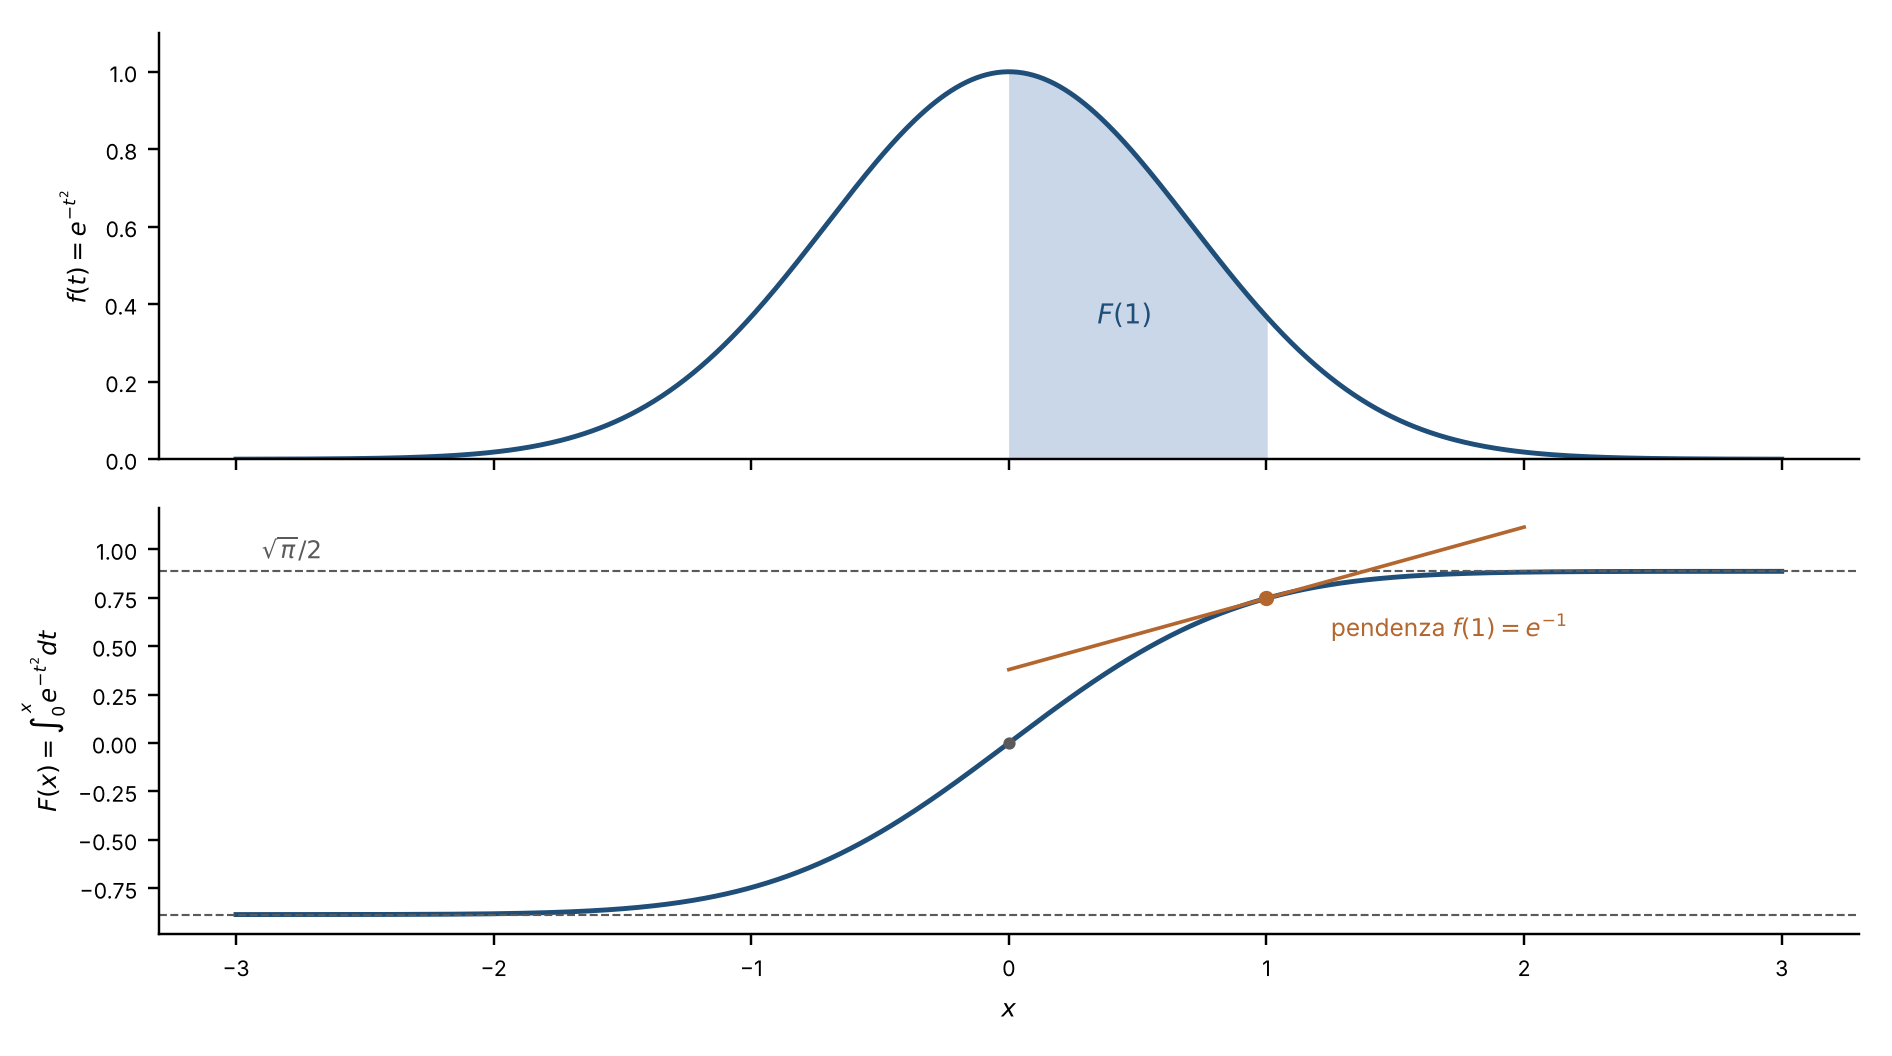
\includegraphics[width=\textwidth]{figure/funzione_integrale.png}
\caption{In alto, la funzione $f(t)=e^{-t^{2}}$ con l'area da $0$ a $x=1$; in basso, la
sua funzione integrale $F(x)=\int_{0}^{x}e^{-t^{2}}dt$, con la retta tangente in $x=1$, di
pendenza $f(1)=e^{-1}$. Dove $f$ è massima, $F$ ha il flesso; l'esistenza degli asintoti
orizzontali sarà dimostrata nel \cref{sec:impropri}, mentre il loro valore $\pm\frac{\sqrt\pi}2$ si
calcola in un corso di Analisi Matematica~2
(\texttt{python/fig\_funzione\_integrale.py}).}
\label{fig:funzione-integrale}
\end{figure}

\begin{notastorica}[Newton, Leibniz e la disputa sulla priorità]
Il legame tra il problema delle tangenti e quello delle aree fu intravisto da diversi
matematici del Seicento: Evangelista Torricelli, James Gregory e soprattutto Isaac
Barrow, che nelle \emph{Lectiones geometricae} (1670) ne diede una formulazione
geometrica. Furono però Isaac Newton, intorno al 1665--1666, e Gottfried Wilhelm
Leibniz, a Parigi, intorno al 1675, a farne lo strumento di un calcolo generale, con
notazioni e regole valide per tutte le curve (Newton, nel 1669, succedette proprio a
Barrow sulla cattedra lucasiana di Cambridge). Nello stesso 1669 Newton raccolse i suoi
metodi nel \emph{De analysi}, stampato soltanto nel 1711: vi mostrava che l'area sotto
una curva, pensata come funzione dell'ascissa, cresce con velocità uguale all'ordinata
(il nostro $F'=f$), e calcolava le aree sviluppando in serie e integrando termine a
termine. Newton
comunicò il risultato a Leibniz in forma cifrata, con l'anagramma dell'epigrafe, nella
lettera del 24 ottobre 1676; Leibniz pubblicò per primo, nel 1684 e nel 1686, sugli
\emph{Acta Eruditorum}. Ne seguì una violenta disputa sulla priorità, che la Royal
Society, presieduta da Newton, chiuse nel 1712 a favore del suo presidente (il rapporto
fu pubblicato nel 1713 nel \emph{Commercium epistolicum}) e che divise
per un secolo i matematici inglesi da quelli del continente. Oggi si riconosce che le
due scoperte furono indipendenti. La parola «integrale» comparve a stampa nel 1690, in
una memoria di Jakob Bernoulli sugli \emph{Acta Eruditorum}; Leibniz, che parlava di
\emph{calculus summatorius}, adottò poi il nome \emph{calculus integralis} proposto da
Johann Bernoulli. La dimostrazione rigorosa che abbiamo seguito, basata sul teorema
della media, è dovuta a Cauchy (1823). Avendo definito l'integrale come limite di somme
(si veda la nota storica del \S\ref{sec:integrale-definito}), Cauchy dovette
\emph{dimostrare} ciò che per i predecessori, per i quali integrare significava trovare
una primitiva, era quasi una definizione.
\end{notastorica}

%% ----------------------------------------------------------------------------
%%  §9.2  Primitive. Formula fondamentale del calcolo integrale
%% ----------------------------------------------------------------------------
\section{Primitive. Formula fondamentale del calcolo integrale}
\label{sec:primitive}

\begin{definizione}[Primitiva]\label{def:primitiva}\index{primitiva}
Sia $f$ una funzione definita in un intervallo $I$. Una funzione $F$ si dice una
\emph{primitiva} di $f$ in $I$ se $F$ è derivabile in $I$ e $F'(x)=f(x)$ per ogni $x\in I$.
\end{definizione}

Ad esempio, una primitiva di $f(x)=x$ in $\R$ è $F(x)=\frac{x^{2}}2$; una primitiva di
$\sen x$ è $-\cos x$; una primitiva di $\frac1x$ nell'intervallo $(0,+\infty)$ è $\log x$.
Con la definizione di primitiva, il teorema fondamentale si enuncia così: \emph{se $f$ è
continua in $[a,b]$, la funzione integrale $F(x)=\int_{a}^{x}f(t)\,dt$ è una primitiva di
$f$}. Più in generale, se $f$ è continua in un intervallo $I$ qualsiasi (aperto,
semiaperto o illimitato) e $c\in I$, la funzione $\int_{c}^{x}f(t)\,dt$ è una primitiva di
$f$ in $I$: basta applicare il \cref{teo:fondamentale} in un intervallo chiuso e
limitato contenuto in $I$ che contenga $c$ e il punto $x$ considerato, con $x$ al suo
interno se $x$ non è un estremo di $I$. Dunque:

\begin{center}
\emph{ogni funzione continua in un intervallo ammette primitive.}
\end{center}

Non tutte le funzioni, però, ammettono primitive, neppure se sono integrabili. La
funzione $f$ che vale $-1$ per $x<0$ e $1$ per $x\ge0$ è integrabile in $[-1,1]$, ma non ha
primitive: se fosse $G'=f$ in $[-1,1]$, la derivata $G'$ non si annullerebbe mai e
cambierebbe segno, contro il lemma di Darboux (\cref{lem:darboux}). Viceversa, esistono
funzioni discontinue che ammettono primitive, come la derivata di $x^{2}\sen\frac1x$
(\cref{oss:f2-non-C1}).

\subsection{Le primitive di una funzione in un intervallo}

Se $F$ è una primitiva di $f$, anche $F+c$ lo è, qualunque sia la costante $c$, perché la
derivata di una costante è nulla. Il teorema seguente afferma che in un intervallo non
ce ne sono altre.

\begin{teorema}[Caratterizzazione delle primitive in un intervallo]
\label{teo:caratterizzazione-primitive}
Se $F$ e $G$ sono due primitive di una stessa funzione $f$ in un intervallo $I$, esiste
una costante $c$ tale che
\begin{equation}\label{eq:primitive-costante}
  G(x)=F(x)+c \qquad\perogni x\in I .
\end{equation}
\end{teorema}

\begin{schema}
\Ipotesi{$I$ intervallo; \ $F'=G'=f$ in $I$.}
\Tesi{$G-F$ è costante in $I$.}
\end{schema}

\begin{strategia}
La differenza $H=G-F$ ha derivata nulla in $I$. Una funzione con derivata nulla in un
intervallo è costante: è una conseguenza del teorema di Lagrange, già dimostrata nel
\cref{cap:applicazioni-derivate}. L'ipotesi che $I$ sia un intervallo serve proprio a
poter applicare il teorema di Lagrange tra due punti qualsiasi.
\end{strategia}

\begin{dimostrazione}
Sia $H=G-F$; allora $H$ è derivabile in $I$ e $H'(x)=G'(x)-F'(x)=f(x)-f(x)=0$ per ogni
$x\in I$. Fissato $x_{0}\in I$, sia $x\in I$ con $x\neq x_{0}$. Poiché $I$ è un intervallo,
contiene l'intervallo chiuso di estremi $x_{0}$ e $x$, nel quale $H$ è continua (perché
derivabile) con derivata nulla; per il \cref{cor:funzioni-costanti}, $H$ è costante in
tale intervallo, e quindi $H(x)=H(x_{0})$. Posto $c=H(x_{0})$, si ha $G(x)=F(x)+c$ per ogni
$x\in I$.
\end{dimostrazione}

L'ipotesi che il dominio sia un intervallo è essenziale. Le funzioni $F(x)=\log\abs x$ e
\[
  G(x)=\begin{cases} \log\abs x+1 & \text{se } x>0,\\ \log\abs x+2 & \text{se } x<0 \end{cases}
\]
hanno entrambe derivata $\frac1x$ in $\R\setminus\set{0}$ (lo verificheremo nella
\eqref{eq:derivata-log-abs}), ma la loro differenza non è costante: su ciascuno dei due
intervalli $(-\infty,0)$ e $(0,+\infty)$ la costante può essere scelta indipendentemente.

\begin{figure}[htb]
\centering
\begin{tikzpicture}
\begin{axis}[name=p1, width=0.52\textwidth, height=5cm, axis lines=middle,
  xmin=-0.4, xmax=6.6, ymin=-2.3, ymax=3.4, xtick=\empty,
  ytick=\empty, title={\scriptsize primitive di $\cos x$: $\sen x+c$}, clip=false]
  \addplot[curva3, domain=-0.3:6.4, samples=100] {sin(deg(x))-1};
  \addplot[curva, domain=-0.3:6.4, samples=100] {sin(deg(x))};
  \addplot[curva2, domain=-0.3:6.4, samples=100] {sin(deg(x))+1};
  \addplot[curva3, domain=-0.3:6.4, samples=100] {sin(deg(x))+2};
  \addplot[tratteggio] coordinates {(1.2,-2.2) (1.2,3.3)};
  \addplot[grigio, thick] coordinates {(0.4,-0.358) (2.0,0.222)};
  \addplot[grigio, thick] coordinates {(0.4,0.642) (2.0,1.222)};
  \addplot[grigio, thick] coordinates {(0.4,1.642) (2.0,2.222)};
  \addplot[grigio, thick] coordinates {(0.4,2.642) (2.0,3.222)};
  \addplot[only marks, mark=*, mark size=1.1pt, grigio] coordinates
    {(1.2,-0.068) (1.2,0.932) (1.2,1.932) (1.2,2.932)};
  \node[font=\scriptsize, anchor=north] at (axis cs:1.2,-2.25) {$x_{0}$};
\end{axis}
\begin{axis}[at={(p1.east)}, anchor=west, xshift=0.7cm, width=0.46\textwidth,
  height=5cm, axis lines=middle, xmin=-0.3, xmax=3.6, ymin=-0.2, ymax=1.35,
  xtick={1.5708,3.1416}, xticklabels={$\frac\pi2$,$\pi$}, ytick={1},
  title={\scriptsize $\int_{0}^{\pi}\sen x\,dx=2$}]
  \addplot[draw=none, fill=blu!22, domain=0:3.1416, samples=60] {sin(deg(x))}
    \closedcycle;
  \addplot[curva, domain=0:3.1416, samples=80] {sin(deg(x))};
  \node[font=\scriptsize, blu] at (axis cs:1.5708,0.42) {area $=2$};
\end{axis}
\end{tikzpicture}
\caption{A sinistra, alcune primitive di $\cos x$: i loro grafici si ottengono l'uno
dall'altro per traslazione verticale, e nello stesso punto $x_{0}$ hanno tangenti
parallele, di pendenza $\cos x_{0}$. A destra, l'area sotto un arco di sinusoide, calcolata
con la formula fondamentale \eqref{eq:formula-fondamentale}.}
\label{fig:primitive}
\end{figure}

\subsection{La formula fondamentale}

Il risultato seguente riconduce il calcolo degli integrali definiti alla ricerca delle
primitive.

\begin{teorema}[Formula fondamentale del calcolo integrale]\label{teo:formula-fondamentale}
\index{formula fondamentale del calcolo integrale}
Sia $f$ una funzione continua in $[a,b]$ e sia $G$ una primitiva di $f$ in $[a,b]$. Allora
\begin{equation}\label{eq:formula-fondamentale}
  \int_{a}^{b}f(x)\,dx=\Bigl[G(x)\Bigr]_{a}^{b}=G(b)-G(a) .
\end{equation}
\end{teorema}

\begin{schema}
\Ipotesi{$f$ continua in $[a,b]$; \ $G'=f$ in $[a,b]$.}
\Tesi{$\int_{a}^{b}f=G(b)-G(a)$.}
\end{schema}

\begin{strategia}
La funzione integrale $F(x)=\int_{a}^{x}f$ è una primitiva di $f$ (teorema fondamentale),
come $G$. Per la caratterizzazione delle primitive, $G=F+c$; la costante si determina
calcolando in $x=a$, dove $F$ si annulla, e la tesi si ottiene calcolando in $x=b$.
\end{strategia}

\begin{dimostrazione}
Per il \cref{teo:fondamentale}, $F(x)=\int_{a}^{x}f(t)\,dt$ è una primitiva di $f$ in
$[a,b]$; per il \cref{teo:caratterizzazione-primitive} esiste una costante $c$ tale che
\[
  G(x)=F(x)+c=c+\int_{a}^{x}f(t)\,dt \qquad\perogni x\in[a,b] .
\]
Per $x=a$ si ottiene $G(a)=c+0=c$; sostituendo, $G(x)=G(a)+\int_{a}^{x}f(t)\,dt$, e per
$x=b$ si ha la tesi.
\end{dimostrazione}

Il simbolo $\bigl[G(x)\bigr]_{a}^{b}$ indica la differenza $G(b)-G(a)$; si scrive anche
$G(x)\big|_{a}^{b}$. La formula vale anche se $a>b$, per la \eqref{eq:estremi-invertiti}.

\begin{esempio}[Primi integrali calcolati con la formula fondamentale]
\label{es:formula-fondamentale}
Ecco alcuni integrali che il \cref{cap:integrali-definiti} non permetteva di calcolare, o
permetteva di calcolare soltanto con fatica.
\begin{enumerate}[label=\textup{(\alph*)}]
  \item Il settore di parabola: $G(x)=\frac{x^{3}}3$ è una primitiva di $x^{2}$, e
  \[
    \int_{0}^{b}x^{2}\,dx=\Bigl[\frac{x^{3}}3\Bigr]_{0}^{b}=\frac{b^{3}}3 .
  \]
  Il risultato di Archimede,
  che ci era costato un paragrafo, si ottiene in una riga.
  \item L'arco di sinusoide (\cref{fig:primitive}, a destra):
  $\int_{0}^{\pi}\sen x\,dx=\bigl[-\cos x\bigr]_{0}^{\pi}=-\cos\pi+\cos0=2$.
  \item Poiché $D\operatorname{arctg}x=\frac1{1+x^{2}}$ \eqref{eq:derivata-arctg},
  $\int_{0}^{1}\frac{dx}{1+x^{2}}=\operatorname{arctg}1-\operatorname{arctg}0=\frac\pi4$: è il
  valore annunciato negli esercizi del \cref{cap:integrali-definiti}, e quindi anche
  $\sum_{k=1}^{n}\frac n{n^{2}+k^{2}}\to\frac\pi4$ (\cref{es:limiti-riemann}).
  \item Poiché $D\,2^{x}=2^{x}\log2$ \eqref{eq:derivata-ax}, una primitiva di $2^{x}$ è
  $\frac{2^{x}}{\log2}$, e $\int_{0}^{1}2^{x}\,dx=\frac{2-1}{\log2}=\frac1{\log2}$, come avevamo
  trovato con le progressioni geometriche (\cref{es:integrale-esponenziale}).
\end{enumerate}
\end{esempio}

\begin{osservazione}[La formula fondamentale senza il teorema fondamentale]
\label{oss:formula-fondamentale-integrabili}
La formula \eqref{eq:formula-fondamentale} vale anche se $f$ è soltanto integrabile in
$[a,b]$, purché abbia una primitiva $G$ in $[a,b]$. Infatti, per ogni partizione
$P=\set{x_{0},\dots,x_{n}}$, il teorema di Lagrange applicato a $G$ in ciascun intervallo
$[x_{k-1},x_{k}]$ fornisce punti $\xi_{k}$ con $G(x_{k})-G(x_{k-1})=f(\xi_{k})\,\Delta x_{k}$, e
sommando (la somma a primo membro è telescopica)
\[
  G(b)-G(a)=\sum_{k=1}^{n}f(\xi_{k})\,\Delta x_{k} ,
\]
che è una somma di Riemann, compresa tra $s(P)$ e $S(P)$. Il numero $G(b)-G(a)$ è dunque un
elemento separatore tra le somme inferiori e superiori di $f$, e poiché $f$ è
integrabile coincide con l'integrale. Questa dimostrazione mostra anche perché la
formula funziona: in una qualsiasi partizione, l'incremento totale di $G$ è la somma
degli incrementi sui singoli intervalli, ciascuno uguale a «derivata per ampiezza».
\end{osservazione}

\begin{idea}[Spazio percorso e velocità]
Se $s(t)$ è la posizione di un velivolo lungo la pista e la velocità $v(t)=s'(t)$ è
continua, la formula fondamentale dà
\begin{equation}\label{eq:spazio-velocita}
  s(t_{1})-s(t_{0})=\int_{t_{0}}^{t_{1}}v(t)\,dt :
\end{equation}
lo spazio percorso è l'area sotto il grafico della velocità. È la giustificazione
promessa nel \cref{cap:integrali-definiti} per la corsa di decollo e per il variometro
dell'aliante: la quota $h(t)$ ha derivata $v_{z}(t)$, e la variazione di quota è
$\int v_{z}\,dt$. Allo stesso modo, il teorema della media per gli integrali diventa il
teorema di Lagrange per la primitiva: $\frac1{b-a}\int_{a}^{b}f=\frac{G(b)-G(a)}{b-a}=G'(\xi)=f(\xi)$
per un $\xi\in(a,b)$, come avevamo anticipato.
\end{idea}

\subsection{Approfondimento: la formula fondamentale per le funzioni regolari a tratti}
\label{subsec:regolari-tratti}

Nelle applicazioni si incontrano spesso funzioni continue che sono derivabili tranne che in
un numero finito di punti, dove il grafico ha un punto angoloso: $\abs x$, la funzione
integrale $\abs x-1$ del \cref{sec:teorema-fondamentale}, o, come vedremo, il momento
flettente di un'ala che porta un motore. Seguendo \cite{giusti}, estendiamo a queste
funzioni la formula fondamentale.

\begin{definizione}[Funzione regolare a tratti]\label{def:regolare-tratti}
\index{funzione!regolare a tratti}
Una funzione $G:[a,b]\to\R$ si dice \emph{regolare a tratti} se esistono punti
$a=z_{0}<z_{1}<\dots<z_{r}=b$ tali che, in ciascuno degli intervalli aperti
$(z_{k-1},z_{k})$, $G$ è derivabile con derivata $G'$ continua e limitata.
\end{definizione}

Nei punti $z_{k}$ la derivata può non esistere. Assegnandole in quei punti valori
arbitrari si ottiene però una funzione limitata e continua tranne che in un numero finito
di punti, quindi integrabile (\cref{es:continua-tratti}), il cui integrale non dipende dai
valori scelti (\cref{es:valore-in-un-punto}): è questo il numero che indichiamo con
$\int_{a}^{b}G'(x)\,dx$.

\begin{teorema}[Formula fondamentale per le funzioni regolari a tratti]
\label{teo:formula-regolari-tratti}
Se $G$ è continua in $[a,b]$ e regolare a tratti, allora
\begin{equation}\label{eq:formula-regolari-tratti}
  \int_{a}^{b}G'(x)\,dx=G(b)-G(a) .
\end{equation}
\end{teorema}

\begin{schema}
\Ipotesi{$G$ continua in $[a,b]$; \ $G$ derivabile, con $G'$ continua e limitata, in
ciascun intervallo $(z_{k-1},z_{k})$.}
\Tesi{$\int_{a}^{b}G'(x)\,dx=G(b)-G(a)$.}
\end{schema}

\begin{strategia}
Per l'additività basta ragionare su un intervallo $[z_{k-1},z_{k}]$, negli estremi del
quale $G$ può non essere derivabile. Ce ne teniamo lontani: in un intervallo $[t,s]$ più
piccolo vale la formula ordinaria; poi facciamo tendere $t$ e $s$ agli estremi, usando
la continuità della funzione integrale e quella di $G$, che è dunque essenziale.
\end{strategia}

\begin{dimostrazione}
Fissato $k$, poniamo $\alpha=z_{k-1}$, $\beta=z_{k}$; sia $g$ una funzione uguale a $G'$
in $(\alpha,\beta)$, con valori arbitrari in $\alpha$ e $\beta$, e sia
$\Phi(x)=\int_{\alpha}^{x}g(t)\,dt$ per $x\in[\alpha,\beta]$. Se $\alpha<t<s<\beta$, la
funzione $G$ è derivabile in $[t,s]$ con derivata continua, e per l'additività e il
\cref{teo:formula-fondamentale}
\[
  \Phi(s)-\Phi(t)=\int_{t}^{s}G'(x)\,dx=G(s)-G(t) .
\]
La funzione $\Phi$ è continua in $[\alpha,\beta]$ (\cref{prop:integrale-lipschitz}), e
così pure $G$, per ipotesi. Facendo tendere $t$ ad $\alpha$ da destra si ottiene
$\Phi(s)=G(s)-G(\alpha)$ per ogni $s\in(\alpha,\beta)$, perché $\Phi(\alpha)=0$; facendo
poi tendere $s$ a $\beta$ da sinistra, $\Phi(\beta)=G(\beta)-G(\alpha)$, cioè
$\int_{z_{k-1}}^{z_{k}}G'=G(z_{k})-G(z_{k-1})$. Sommando su $k$ e usando l'additività
(\cref{teo:additivita}), il secondo membro è una somma telescopica che vale $G(b)-G(a)$.
\end{dimostrazione}

\begin{osservazione}[La continuità di $G$ è essenziale]\label{oss:regolari-tratti-salti}
La funzione segno $G$, che vale $-1$ per $x<0$, $0$ in $0$ e $1$ per $x>0$, è regolare a tratti
in $[-1,1]$, con derivata nulla per $x\neq0$: dunque $\int_{-1}^{1}G'=0$, mentre
$G(1)-G(-1)=2$. La differenza è il salto in $0$: la derivata «non vede» i salti. In
generale, se $G$ è regolare a tratti, continua in $a$ e in $b$, e nei punti interni
$z_{k}$ ha limiti destro e sinistro, la stessa dimostrazione (dove ora, per $t\to z_{k-1}^{+}$
e $s\to z_{k}^{-}$, compaiono i limiti laterali di $G$) dà
\[
  \int_{a}^{b}G'(x)\,dx=G(b)-G(a)-\sum_{k=1}^{r-1}\sigma_{k}, \qquad
  \sigma_{k}=\lim_{x\to z_{k}^{+}}G(x)-\lim_{x\to z_{k}^{-}}G(x) .
\]
\end{osservazione}

\begin{esempio}[Una funzione integranda con un salto]\label{es:integranda-salto}
Sia $f(x)=-1$ per $x<0$ e $f(x)=x$ per $x\ge0$. La funzione $f$ non ha primitive in
$[-1,2]$ (se fosse $H'=f$, la derivata di $H(x)+\frac x2$ non si annullerebbe mai e
cambierebbe segno, contro il \cref{lem:darboux}), ma fuori dall'origine è la derivata di
\[
  G(x)=\begin{cases} -x & \text{se } x<0,\\[2pt] \dfrac{x^{2}}2+c & \text{se } x\ge0, \end{cases}
\]
qualunque sia la costante $c$. Con $c=0$ la funzione $G$ è continua e regolare a tratti, e
per il \cref{teo:formula-regolari-tratti} $\int_{-1}^{2}f=G(2)-G(-1)=2-1=1$, come conferma
il calcolo spezzato in $0$. Con $c\neq0$, invece, $G$ ha in $0$ il salto $\sigma_{1}=c$, e
$G(2)-G(-1)=1+c$ è sbagliato proprio di $c$: le costanti dei diversi tratti vanno scelte
in modo da «incollare» i pezzi di $G$ con continuità.
\end{esempio}

\begin{notastorica}[Derivate non integrabili: Volterra e Lebesgue]
Nell'\cref{oss:formula-fondamentale-integrabili} e nel \cref{teo:formula-regolari-tratti}
abbiamo supposto la derivata integrabile. L'ipotesi sembra superflua quando la derivata è
limitata; invece nel 1881 Vito Volterra, allora studente di Ulisse Dini alla Scuola
Normale di Pisa, costruì una funzione derivabile in ogni punto, con derivata limitata ma
non integrabile secondo Riemann, perché discontinua in un insieme che non ha misura
nulla (nel senso della nota storica del \S\ref{sec:integrabilita-continue}): per essa il
primo membro della formula fondamentale non esiste. La questione fu risolta da Henri
Lebesgue: con il suo integrale, introdotto nella tesi del 1902, ogni derivata limitata è
integrabile e la formula $\int_{a}^{b}G'=G(b)-G(a)$ vale sempre. Non a caso le sue lezioni
del 1904 si intitolano \emph{Leçons sur l'intégration et la recherche des fonctions
primitives}: ritrovare una funzione dalla sua derivata è il problema di questo capitolo.
\end{notastorica}

%% ----------------------------------------------------------------------------
%%  §9.3  L'integrale indefinito. Integrali immediati. Decomposizione in somma
%% ----------------------------------------------------------------------------
\section{L'integrale indefinito}
\label{sec:integrale-indefinito}

Nel paragrafo precedente abbiamo ricondotto il calcolo di un integrale definito alla
ricerca di una primitiva della funzione integranda. È perciò naturale porre la
definizione seguente.

\begin{definizione}[Integrale indefinito]\label{def:integrale-indefinito}
\index{integrale indefinito}
Sia $f$ una funzione continua in un intervallo $I$. L'insieme di tutte le primitive di
$f$ in $I$ si chiama \emph{integrale indefinito} di $f$ e si indica con il simbolo
\begin{equation}\label{eq:integrale-indefinito}
  \int f(x)\,dx .
\end{equation}
\end{definizione}

Per il \cref{teo:caratterizzazione-primitive}, se $F$ è una primitiva di $f$ in $I$,
\begin{equation}\label{eq:integrale-indefinito-c}
  \int f(x)\,dx=F(x)+c ,
\end{equation}
dove $c$ è una costante arbitraria: la scrittura significa che l'insieme delle
primitive è $\set{F+c \tc c\in\R}$. C'è una differenza sostanziale tra l'integrale
definito $\int_{a}^{b}f(x)\,dx$, che è un \emph{numero}, e l'integrale indefinito $\int f(x)\,dx$,
che è un \emph{insieme di funzioni}; il legame tra i due è la formula fondamentale
\eqref{eq:formula-fondamentale}. Nella pratica si scrive $\int f(x)\,dx=F(x)+c$ e si dice,
con un abuso di linguaggio, che $F$ «è» l'integrale indefinito di $f$.

Poiché la derivata di una somma è la somma delle derivate e la derivata di $cF$ è
$cF'$ (\cref{teo:operazioni-derivate}), se $F$ e $G$ sono primitive di $f$ e $g$, allora
$F+G$ è una primitiva di $f+g$ e $cF$ è una primitiva di $cf$. In termini di integrali
indefiniti,
\begin{equation}\label{eq:linearita-indefinito}
\begin{gathered}
  \int\bigl[f(x)+g(x)\bigr]dx=\int f(x)\,dx+\int g(x)\,dx,\\
  \int c\,f(x)\,dx=c\int f(x)\,dx \quad (c\neq0),
\end{gathered}
\end{equation}
in analogia con la linearità dell'integrale definito (\cref{teo:linearita}). Le
uguaglianze vanno intese a meno di costanti additive.

\subsection{Integrali immediati}

Leggendo da destra a sinistra la tabella delle derivate elementari
(\cref{tab:derivate-elementari}) e le derivate delle funzioni trigonometriche inverse
\eqref{eq:derivata-arcsen}, \eqref{eq:derivata-arctg} si ottengono gli \emph{integrali immediati} della
\cref{tab:integrali-immediati}. Ciascuno si verifica derivando il secondo membro, e
ciascuno vale in ogni intervallo in cui la funzione integranda è continua.

\begin{table}[htb]
\centering
\renewcommand{\arraystretch}{1.9}
\begin{tabular}{@{}l@{\qquad}l@{}}
\toprule
$\displaystyle\int x^{b}\,dx=\frac{x^{b+1}}{b+1}+c \quad (b\neq-1)$ &
$\displaystyle\int\frac{dx}x=\log\abs x+c$\\
$\displaystyle\int e^{x}\,dx=e^{x}+c$ &
$\displaystyle\int a^{x}\,dx=\frac{a^{x}}{\log a}+c \quad (a>0,\ a\neq1)$\\
$\displaystyle\int\sen x\,dx=-\cos x+c$ &
$\displaystyle\int\cos x\,dx=\sen x+c$\\
$\displaystyle\int\frac{dx}{\cos^{2}x}=\tg x+c$ &
$\displaystyle\int\frac{dx}{\sqrt{1-x^{2}}}=\arcsen x+c$\\
$\displaystyle\int\frac{dx}{1+x^{2}}=\operatorname{arctg}x+c$ & \\
\bottomrule
\end{tabular}
\caption{Integrali immediati. Ciascuna formula vale in ogni intervallo in cui la
funzione integranda è continua: ad esempio, la prima con $b=-2$ vale in $(-\infty,0)$ e
in $(0,+\infty)$, la seconda in ciascuno dei due intervalli che non contengono lo zero.}
\label{tab:integrali-immediati}
\end{table}

A proposito del logaritmo, osserviamo che
\begin{equation}\label{eq:derivata-log-abs}
  D\log\abs x=\frac1x \qquad\perogni x\neq0 .
\end{equation}
Per $x>0$ è la \eqref{eq:derivata-log}. Per $x<0$ si ha $\abs x=-x$, e per la regola di
derivazione delle funzioni composte
\[
  D\log\abs x=D\log(-x)=\frac1{-x}\cdot(-1)=\frac1x \qquad (x<0) .
\]
Dunque $\int\frac{dx}x=\log\abs x+c$, intendendo che l'integrale è considerato in un intervallo
che non contiene il punto $x=0$.

\subsection{Integrali immediati di funzioni composte}

Molti integrali si riconducono a quelli della tabella grazie alla regola di derivazione
delle funzioni composte (\cref{teo:derivata-composta}). Se $G$ è una primitiva di $g$ e
$\varphi$ è derivabile, allora $D\,G(\varphi(x))=g(\varphi(x))\,\varphi'(x)$, cioè
\begin{equation}\label{eq:composta-indefinito}
  \int g\bigl(\varphi(x)\bigr)\,\varphi'(x)\,dx=G\bigl(\varphi(x)\bigr)+c .
\end{equation}
In particolare, per una funzione $\varphi$ derivabile (positiva nella prima formula se $b$
non è intero, non nulla se $b$ è intero negativo; non nulla nella seconda),
\begin{equation}\label{eq:integrali-composti}
\begin{aligned}
  \int\varphi(x)^{b}\,\varphi'(x)\,dx&=\frac{\varphi(x)^{b+1}}{b+1}+c \qquad (b\neq-1),\\
  \int\frac{\varphi'(x)}{\varphi(x)}\,dx&=\log\abs{\varphi(x)}+c,\\
  \int e^{\varphi(x)}\varphi'(x)\,dx&=e^{\varphi(x)}+c,\\
  \int\frac{\varphi'(x)}{1+\varphi^{2}(x)}\,dx&=\operatorname{arctg}\varphi(x)+c .
\end{aligned}
\end{equation}
Il caso più frequente è quello di un argomento lineare, $\varphi(x)=\alpha x+\beta$ con
$\alpha\neq0$: allora $\varphi'=\alpha$, e
\begin{equation}\label{eq:argomento-lineare}
  \int g(\alpha x+\beta)\,dx=\frac1\alpha\,G(\alpha x+\beta)+c ;
\end{equation}
ad esempio, $\int\cos2x\,dx=\frac12\sen2x+c$ e $\int e^{-3x}\,dx=-\frac13e^{-3x}+c$.

\begin{esempio}[Integrali di funzioni composte]\label{es:integrali-composti}
\begin{enumerate}[label=\textup{(\alph*)}]
  \item In $\tg x=\frac{\sen x}{\cos x}$ il numeratore è, a meno del segno, la derivata
  del denominatore:
  \begin{equation}\label{eq:integrale-tg}
    \int\tg x\,dx=-\int\frac{-\sen x}{\cos x}\,dx=-\log\abs{\cos x}+c .
  \end{equation}
  \item $\int\frac x{1+x^{2}}\,dx=\frac12\int\frac{2x}{1+x^{2}}\,dx=\frac12\log(1+x^{2})+c$ (il valore
  assoluto non serve, perché $1+x^{2}>0$).
  \item $\int x\,e^{x^{2}}dx=\frac12\int e^{x^{2}}\,2x\,dx=\frac12e^{x^{2}}+c$.
  \item $\int\sen x\cos x\,dx=\int\sen x\,D(\sen x)\,dx=\frac12\sen^{2}x+c$.
  \item $\int\frac{dx}{x\log x}=\int\frac{1/x}{\log x}\,dx=\log\abs{\log x}+c$, in $(0,1)$ o in
  $(1,+\infty)$.
\end{enumerate}
\end{esempio}

\subsection{Integrazione per decomposizione in somma}

In molti casi il calcolo dell'integrale indefinito di una funzione si riconduce a quello
di integrali già noti, o più semplici, decomponendo la funzione integranda nella somma
di due o più funzioni e applicando la linearità \eqref{eq:linearita-indefinito}.

\begin{esempio}[Quattro decomposizioni]\label{es:decomposizione}
\begin{enumerate}[label=\textup{(\alph*)}]
  \item Sommando e sottraendo $1$ al numeratore:
  \[
  \begin{aligned}
    \int\frac x{x+1}\,dx&=\int\frac{x+1-1}{x+1}\,dx=\int\Bigl(1-\frac1{x+1}\Bigr)dx\\
    &=x-\log\abs{x+1}+c .
  \end{aligned}
  \]
  \item Poiché $\tg^{2}x=\frac{\sen^{2}x}{\cos^{2}x}=\frac{1-\cos^{2}x}{\cos^{2}x}=\frac1{\cos^{2}x}-1$,
  \[
    \int\tg^{2}x\,dx=\int\Bigl(\frac1{\cos^{2}x}-1\Bigr)dx=\tg x-x+c .
  \]
  \item Scrivendo $1=\sen^{2}x+\cos^{2}x$ al numeratore, la frazione si scinde:
  \[
  \begin{aligned}
    \int\frac{dx}{\sen x\cos x}&=\int\Bigl(\frac{\sen x}{\cos x}+\frac{\cos x}{\sen x}\Bigr)dx\\
    &=-\log\abs{\cos x}+\log\abs{\sen x}+c=\log\abs{\tg x}+c .
  \end{aligned}
  \]
  \item Dalla formula di duplicazione $\cos2x=\cos^{2}x-\sen^{2}x=1-2\sen^{2}x$
  \eqref{eq:duplicazione} si ha $\sen^{2}x=\frac{1-\cos2x}2$, e per la
  \eqref{eq:argomento-lineare}
  \begin{equation}\label{eq:integrale-sen2}
  \begin{split}
    \int\sen^{2}x\,dx&=\frac12\int(1-\cos2x)\,dx=\frac x2-\frac{\sen2x}4+c\\
    &=\frac12\,(x-\sen x\cos x)+c ,
  \end{split}
  \end{equation}
  dove nell'ultimo passaggio si è usata la duplicazione $\sen2x=2\sen x\cos x$. Ne segue
  \begin{equation}\label{eq:integrale-cos2}
    \int\cos^{2}x\,dx=\int(1-\sen^{2}x)\,dx=\frac12\,(x+\sen x\cos x)+c .
  \end{equation}
\end{enumerate}
\end{esempio}

Il calcolo simbolico permette di verificare rapidamente un integrale indefinito. Il
programma seguente usa \texttt{sympy}: per ciascuna funzione calcola una primitiva $F$
e controlla che $F'-f$ si semplifichi a zero.

\begin{python}[Integrali indefiniti con sympy, e la loro verifica]
import sympy as sp

x = sp.symbols("x", real=True)
esempi = [x / (x + 1), sp.tan(x)**2, sp.sin(x)**2, sp.tan(x),
          x * sp.exp(x**2), 1 / (x * sp.log(x))]
for f in esempi:
    F = sp.integrate(f, x)
    verifica = sp.simplify(sp.diff(F, x) - f)
    print(f"f = {f}")
    print(f"    F = {F}      F' - f = {verifica}")
\end{python}
\begin{risultato}
f = x/(x + 1)
    F = x - log(x + 1)      F' - f = 0
f = tan(x)**2
    F = -x + sin(x)/cos(x)      F' - f = 0
f = sin(x)**2
    F = x/2 - sin(x)*cos(x)/2      F' - f = 0
f = tan(x)
    F = -log(cos(x))      F' - f = 0
f = x*exp(x**2)
    F = exp(x**2)/2      F' - f = 0
f = 1/(x*log(x))
    F = log(log(x))      F' - f = 0
\end{risultato}

Si osservi che \texttt{sympy} non scrive la costante arbitraria e scrive $\log(x+1)$,
$\log(\cos x)$, $\log(\log x)$ senza valore assoluto: le sue primitive sono corrette
negli intervalli in cui l'argomento del logaritmo è positivo (per $\cos x<0$, ad
esempio, \texttt{sympy} lavora in campo complesso). Il risultato di un programma di
calcolo simbolico va sempre letto con senso critico, controllando l'intervallo in cui
vale.

\begin{notastorica}[Le tavole degli integrali e i limiti del calcolo]
Tra le prime raccolte sistematiche di integrali indefiniti vi furono quelle delle
\emph{Institutiones calculi integralis} di Eulero (1768--1770), che fissarono per più di
un secolo i metodi che studieremo nei prossimi paragrafi. Ci si accorse presto che
alcune funzioni elementari molto semplici, come $e^{-x^{2}}$, $\frac{\sen x}x$, $\frac1{\log x}$,
resistevano a ogni tentativo di integrazione: Joseph Liouville dimostrò, in una serie di
memorie del 1833--1841, che le loro primitive non si possono esprimere mediante un numero
finito di funzioni elementari. Le primitive esistono (per il teorema fondamentale), ma
definiscono funzioni nuove, come la funzione degli errori $\operatorname{erf}$, che si
calcolano numericamente. Nel 1969 Robert Risch pubblicò un algoritmo (completo nel caso delle funzioni
trascendenti) che decide se una funzione elementare ha una primitiva elementare e, in
caso affermativo, la calcola: i programmi di calcolo simbolico come \texttt{sympy} ne
implementano versioni parziali, affiancate da procedimenti euristici.
\end{notastorica}

%% ----------------------------------------------------------------------------
%%  §9.4  Integrazione delle funzioni razionali
%% ----------------------------------------------------------------------------
\section{Integrazione delle funzioni razionali}
\label{sec:razionali}

È sempre possibile, in linea di principio, calcolare per decomposizione in somma
l'integrale indefinito delle \emph{funzioni razionali}, cioè delle funzioni che sono
rapporto di due polinomi:
\begin{equation}\label{eq:funzione-razionale}
  \frac{f(x)}{g(x)}=\frac{a_{m}x^{m}+a_{m-1}x^{m-1}+\dots+a_{1}x+a_{0}}
  {b_{n}x^{n}+b_{n-1}x^{n-1}+\dots+b_{1}x+b_{0}}, \qquad a_{m},b_{n}\neq0 .
\end{equation}
Il procedimento si svolge in due tempi: prima ci si riconduce al caso in cui il grado del
numeratore è minore di quello del denominatore, poi si scompone la frazione in frazioni
«semplici», i cui integrali sono immediati.

\subsection{La divisione tra polinomi}

Se $m\ge n$, si esegue la \emph{divisione} tra i polinomi $f$ e $g$: come si dimostra in
algebra (per induzione sul grado di $f$), esistono e sono unici due polinomi $q$, il
\emph{quoziente}, e $r$, il \emph{resto}, con $r$ nullo oppure di grado minore di $n$, tali
che
\begin{equation}\label{eq:divisione-polinomi}
  f(x)=g(x)\,q(x)+r(x), \qquad\text{cioè}\qquad \frac{f(x)}{g(x)}=q(x)+\frac{r(x)}{g(x)} .
\end{equation}
Il polinomio $q$ si integra immediatamente, e resta da integrare la funzione razionale
$\frac rg$, nella quale il grado del numeratore è minore di quello del denominatore.

\begin{esempio}[Una divisione]\label{es:divisione-polinomi}
Dividiamo $f(x)=x^{5}-3x^{4}+x+3$ per $g(x)=x^{2}-1$, procedendo come nella divisione tra
numeri naturali: a ogni passo si divide il termine di grado massimo del dividendo
parziale per $x^{2}$, si moltiplica il risultato per $g$ e lo si sottrae:
\[
\begin{aligned}
  x^{5}-3x^{4}+x+3-x^{3}(x^{2}-1)&=-3x^{4}+x^{3}+x+3,\\
  -3x^{4}+x^{3}+x+3+3x^{2}(x^{2}-1)&=x^{3}-3x^{2}+x+3,\\
  x^{3}-3x^{2}+x+3-x(x^{2}-1)&=-3x^{2}+2x+3,\\
  -3x^{2}+2x+3+3(x^{2}-1)&=2x .
\end{aligned}
\]
Il quoziente è $q(x)=x^{3}-3x^{2}+x-3$ e il resto è $r(x)=2x$. Poiché $2x$ è la derivata
di $x^{2}-1$,
\[
\begin{aligned}
  \int\frac{x^{5}-3x^{4}+x+3}{x^{2}-1}\,dx&=\int(x^{3}-3x^{2}+x-3)\,dx
  +\int\frac{2x}{x^{2}-1}\,dx\\
  &=\frac{x^{4}}4-x^{3}+\frac{x^{2}}2-3x+\log\abs{x^{2}-1}+c .
\end{aligned}
\]
\end{esempio}

\subsection{Denominatore di secondo grado}

Consideriamo ora una funzione razionale $\frac{r(x)}{g(x)}$ con $g$ di secondo grado e $r$ di
grado al più uno. Raccogliendo il coefficiente direttore di $g$ ci si riduce al caso
\begin{equation}\label{eq:razionale-secondo-grado}
  \frac{mx+n}{x^{2}+px+q}, \qquad \Delta=p^{2}-4q ,
\end{equation}
e occorre distinguere tre casi, secondo che l'equazione $x^{2}+px+q=0$ abbia due radici
reali distinte, due radici coincidenti, o nessuna radice reale.

\begin{proposizione}[Integrali delle frazioni con denominatore di secondo grado]
\label{prop:razionali-secondo-grado}
Siano $m,n,p,q\in\R$ e $\Delta=p^{2}-4q$.
\begin{enumerate}[label=\textup{(\roman*)}]
  \item Se $\Delta>0$ e $x_{1}\neq x_{2}$ sono le radici di $x^{2}+px+q$, esistono e sono unici
  $A,B\in\R$ tali che
  \begin{equation}\label{eq:fratti-semplici-distinte}
  \begin{gathered}
    \frac{mx+n}{(x-x_{1})(x-x_{2})}=\frac A{x-x_{1}}+\frac B{x-x_{2}},\\
    A=\frac{mx_{1}+n}{x_{1}-x_{2}}, \qquad B=\frac{mx_{2}+n}{x_{2}-x_{1}},
  \end{gathered}
  \end{equation}
  e quindi l'integrale vale $A\log\abs{x-x_{1}}+B\log\abs{x-x_{2}}+c$.
  \item Se $\Delta=0$ e $x_{1}$ è la radice doppia,
  \begin{equation}\label{eq:fratti-semplici-doppia}
    \int\frac{mx+n}{(x-x_{1})^{2}}\,dx=m\log\abs{x-x_{1}}-\frac{mx_{1}+n}{x-x_{1}}+c .
  \end{equation}
  \item Se $\Delta<0$, posto $\delta=\frac{\sqrt{-\Delta}}2>0$,
  \begin{equation}\label{eq:fratti-semplici-complesse}
  \begin{split}
    \int\frac{mx+n}{x^{2}+px+q}\,dx&=\frac m2\log\bigl(x^{2}+px+q\bigr)\\
    &\quad+\frac{n-\frac{mp}2}{\delta}\,\operatorname{arctg}\frac{x+\frac p2}\delta+c .
  \end{split}
  \end{equation}
\end{enumerate}
\end{proposizione}

\begin{schema}
\Ipotesi{$\frac{mx+n}{x^{2}+px+q}$, con discriminante $\Delta$ positivo, nullo o negativo.}
\Tesi{le decomposizioni e le primitive \eqref{eq:fratti-semplici-distinte},
\eqref{eq:fratti-semplici-doppia}, \eqref{eq:fratti-semplici-complesse}, ciascuna valida in
ogni intervallo in cui il denominatore non si annulla.}
\end{schema}

\begin{strategia}
Nel primo caso si cercano $A$ e $B$ imponendo che la somma delle due frazioni, ridotta
allo stesso denominatore, abbia numeratore $mx+n$: è un'identità tra polinomi, che basta
valutare nelle radici per trovare $A$ e $B$. Nel secondo caso si scrive il numeratore come
$m(x-x_{1})+(mx_{1}+n)$. Nel terzo il denominatore non si scompone; si scrive il numeratore
come multiplo della derivata $2x+p$ del denominatore (che dà un logaritmo) più una
costante, e si completa il quadrato al denominatore, che diventa $(x+\frac p2)^{2}+\delta^{2}$
(che dà un arcotangente).
\end{strategia}

\begin{dimostrazione}
(i) Riducendo allo stesso denominatore, la \eqref{eq:fratti-semplici-distinte} equivale a
\[
  mx+n=A(x-x_{2})+B(x-x_{1}) \qquad\text{per ogni } x\neq x_{1},x_{2} .
\]
I due membri sono polinomi di grado al più uno che coincidono in infiniti punti, quindi
hanno gli stessi coefficienti e coincidono per ogni $x$ (la differenza è un polinomio
di grado al più uno con più di una radice, dunque nullo). Ponendo $x=x_{1}$ si ottiene
$mx_{1}+n=A(x_{1}-x_{2})$, e ponendo $x=x_{2}$ si ottiene $mx_{2}+n=B(x_{2}-x_{1})$: $A$ e $B$ sono
determinati univocamente come nella \eqref{eq:fratti-semplici-distinte}; con tali valori
l'identità è verificata, perché due polinomi di grado al più uno che coincidono in due
punti distinti sono uguali. L'integrale segue da $\int\frac{dx}{x-x_{i}}=\log\abs{x-x_{i}}+c$.

(ii) Si ha $mx+n=m(x-x_{1})+(mx_{1}+n)$, e quindi
$\frac{mx+n}{(x-x_{1})^{2}}=\frac m{x-x_{1}}+\frac{mx_{1}+n}{(x-x_{1})^{2}}$; poiché
$\int(x-x_{1})^{-2}dx=-(x-x_{1})^{-1}+c$, si ottiene la \eqref{eq:fratti-semplici-doppia}.

(iii) Scriviamo $mx+n=\frac m2(2x+p)+\bigl(n-\frac{mp}2\bigr)$. Il primo addendo dà, per la
seconda delle \eqref{eq:integrali-composti}, $\frac m2\log(x^{2}+px+q)$, senza valore
assoluto perché il denominatore, privo di radici reali, è sempre positivo. Per il
secondo, completiamo il quadrato:
\[
  x^{2}+px+q=\Bigl(x+\frac p2\Bigr)^{2}+q-\frac{p^{2}}4=\Bigl(x+\frac p2\Bigr)^{2}+\delta^{2}
  =\delta^{2}\Bigl[1+\Bigl(\frac{x+p/2}\delta\Bigr)^{2}\Bigr] ,
\]
con $\delta^{2}=q-\frac{p^{2}}4=-\frac\Delta4>0$. Per la \eqref{eq:argomento-lineare} con
$\alpha=\frac1\delta$,
\[
\begin{aligned}
  \int\frac{dx}{x^{2}+px+q}&=\frac1{\delta^{2}}\int\frac{dx}{1+\bigl(\frac{x+p/2}\delta\bigr)^{2}}
  =\frac1{\delta^{2}}\cdot\delta\,\operatorname{arctg}\frac{x+p/2}\delta+c\\
  &=\frac1\delta\operatorname{arctg}\frac{x+p/2}\delta+c ,
\end{aligned}
\]
e la \eqref{eq:fratti-semplici-complesse} segue per la linearità.
\end{dimostrazione}

\begin{esempio}[I tre casi]\label{es:tre-casi}
\begin{enumerate}[label=\textup{(\alph*)}]
  \item $\Delta>0$. Le radici di $x^{2}-x-2$ sono $x_{1}=-1$ e $x_{2}=2$. Per la
  \eqref{eq:fratti-semplici-distinte} con $m=1$, $n=7$: $A=\frac{-1+7}{-3}=-2$,
  $B=\frac{2+7}3=3$, e
  \[
  \begin{aligned}
    \int\frac{x+7}{x^{2}-x-2}\,dx&=\int\Bigl(\frac{-2}{x+1}+\frac3{x-2}\Bigr)dx\\
    &=-2\log\abs{x+1}+3\log\abs{x-2}+c .
  \end{aligned}
  \]
  \item $\Delta=0$. Per $\frac x{x^{2}+2x+1}=\frac x{(x+1)^{2}}$ si ha $x_{1}=-1$, $m=1$, $n=0$:
  \[
    \int\frac x{(x+1)^{2}}\,dx=\int\Bigl(\frac1{x+1}-\frac1{(x+1)^{2}}\Bigr)dx
    =\log\abs{x+1}+\frac1{x+1}+c .
  \]
  \item $\Delta<0$. Per $\frac{1-2x}{x^{2}+2x+5}$ si ha $p=2$, $q=5$, $\delta=2$, $m=-2$, $n=1$:
  \[
    \int\frac{1-2x}{x^{2}+2x+5}\,dx=-\log(x^{2}+2x+5)+\frac32\operatorname{arctg}\frac{x+1}2+c .
  \]
  Allo stesso modo, per $\frac x{x^{2}+x+1}$ ($p=q=1$, $\delta=\frac{\sqrt3}2$, $m=1$, $n=0$),
  \[
    \int\frac x{x^{2}+x+1}\,dx=\frac12\log(x^{2}+x+1)-\frac{\sqrt3}3\operatorname{arctg}
    \frac{2x+1}{\sqrt3}+c .
  \]
\end{enumerate}
\end{esempio}

\subsection{Denominatori di grado superiore}

Il metodo si estende a denominatori di grado qualsiasi, purché se ne conoscano
esplicitamente le radici. Si dimostra in algebra (è una conseguenza del teorema
fondamentale dell'algebra, ricordato nel \cref{cap:complementi}) che ogni polinomio
reale si scompone nel prodotto di fattori di primo grado $x-x_{i}$ e di fattori di secondo
grado $x^{2}+px+q$ con $\Delta<0$, eventualmente ripetuti; e che ogni funzione razionale con
il numeratore di grado minore del denominatore è somma di \emph{fratti semplici} del
tipo
\[
  \frac A{(x-x_{i})^{k}}, \qquad \frac{Bx+C}{(x^{2}+px+q)^{k}} ,
\]
uno per ogni potenza di ciascun fattore che compare nel denominatore. Le costanti si
determinano, come nella \cref{prop:razionali-secondo-grado}, imponendo l'identità dei
numeratori.

\begin{esempio}[Un denominatore di quarto grado]\label{es:quarto-grado}
Dividendo il numeratore per il denominatore,
$\frac{x^{5}-x+1}{x^{4}+x^{2}}=x-\frac{x^{3}+x-1}{x^{4}+x^{2}}$. Il denominatore è
$x^{2}(x^{2}+1)$, con il fattore $x$ ripetuto due volte e il fattore irriducibile $x^{2}+1$;
cerchiamo dunque
\[
  \frac{x^{3}+x-1}{x^{2}(x^{2}+1)}=\frac Ax+\frac B{x^{2}}+\frac{C+Dx}{x^{2}+1} .
\]
Riducendo allo stesso denominatore e uguagliando i coefficienti dei numeratori
($x^{3}+x-1=Ax(x^{2}+1)+B(x^{2}+1)+(C+Dx)x^{2}$) si trova $A=C=1$, $B=-1$, $D=0$, e quindi
\[
  \int\frac{x^{5}-x+1}{x^{4}+x^{2}}\,dx=\frac{x^{2}}2-\log\abs x-\frac1x-\operatorname{arctg}x+c .
\]
\end{esempio}

\begin{python}[Divisione, fratti semplici e integrazione con sympy]
import sympy as sp

x = sp.symbols("x", real=True)
q, r = sp.div(x**5 - 3*x**4 + x + 3, x**2 - 1, x)
print("quoziente:", q, "   resto:", r)
for f in [(x + 7) / (x**2 - x - 2), x / (x**2 + 2*x + 1),
          (1 - 2*x) / (x**2 + 2*x + 5),
          (x**5 - x + 1) / (x**4 + x**2)]:
    print("f =", f)
    print("    fratti semplici:", sp.apart(f, x))
    print("    integrale:      ", sp.integrate(f, x))
\end{python}
\begin{risultato}
quoziente: x**3 - 3*x**2 + x - 3    resto: 2*x
f = (x + 7)/(x**2 - x - 2)
    fratti semplici: -2/(x + 1) + 3/(x - 2)
    integrale:       3*log(x - 2) - 2*log(x + 1)
f = x/(x**2 + 2*x + 1)
    fratti semplici: 1/(x + 1) - 1/(x + 1)**2
    integrale:       log(x + 1) + 1/(x + 1)
f = (1 - 2*x)/(x**2 + 2*x + 5)
    fratti semplici: -(2*x - 1)/(x**2 + 2*x + 5)
    integrale:       -log(x**2 + 2*x + 5) + 3*atan(x/2 + 1/2)/2
f = (x**5 - x + 1)/(x**4 + x**2)
    fratti semplici: x - 1/(x**2 + 1) - 1/x + x**(-2)
    integrale:       x**2/2 - log(x) - atan(x) - 1/x
\end{risultato}

Il calcolo simbolico conferma le decomposizioni e le primitive (ancora una volta senza
valori assoluti nei logaritmi). Si noti però che il metodo richiede le radici del
denominatore: per un polinomio di grado elevato esse si calcolano, in generale, soltanto
numericamente, e la decomposizione in fratti semplici diventa un procedimento
approssimato.

\begin{notastorica}[Leibniz, Johann Bernoulli e i fratti semplici]
Il metodo dei fratti semplici fu pubblicato quasi contemporaneamente, nel 1702, da
Leibniz e da Johann Bernoulli sugli \emph{Acta Eruditorum}. Leibniz incontrò una
difficoltà che lo portò ad affermare, erroneamente, che non tutte le funzioni razionali
si possono integrare con logaritmi e arcotangenti: non riusciva a scomporre $x^{4}+1$ in
fattori reali di secondo grado. A posteriori l'errore è evidente:
$x^{4}+1=(x^{2}+\sqrt2\,x+1)(x^{2}-\sqrt2\,x+1)$, come si verifica moltiplicando. Il
problema fu risolto in generale soltanto dal teorema fondamentale dell'algebra, che nacque
dunque come questione di calcolo integrale: il primo tentativo di dimostrarlo, di Jean Le
Rond d'Alembert (1746), compare in una memoria intitolata \emph{Recherches sur le calcul
intégral}. La prima dimostrazione sostanzialmente completa, pubblicata da Gauss nel 1799,
conteneva una lacuna topologica colmata da Alexander Ostrowski nel 1920. In Inghilterra la
scuola di Newton seguiva un'altra strada: sviluppava in serie di potenze la funzione
integranda e integrava termine a termine, senza bisogno di scomporre il denominatore. Il
metodo era efficace per i calcoli numerici, ma non dava le formule chiuse in termini di
logaritmi e arcotangenti cercate dai continentali.
\end{notastorica}

%% ----------------------------------------------------------------------------
%%  §9.5  Integrazione per parti
%% ----------------------------------------------------------------------------
\section{Integrazione per parti}
\label{sec:per-parti}

Il metodo di integrazione per decomposizione in somma si basa sulla regola di
derivazione della somma; il metodo di integrazione per parti, che descriviamo ora, si
basa sulla regola di derivazione del prodotto.

\begin{teorema}[Formula di integrazione per parti]\label{teo:per-parti}
\index{integrazione!per parti}
Se $f$ e $g$ sono due funzioni derivabili con derivata continua in un intervallo $I$,
risulta
\begin{equation}\label{eq:per-parti}
  \int f(x)\,g'(x)\,dx=f(x)\,g(x)-\int f'(x)\,g(x)\,dx .
\end{equation}
\end{teorema}

\begin{schema}
\Ipotesi{$f$, $g$ derivabili in $I$, con $f'$, $g'$ continue.}
\Tesi{$\int fg'\,dx=fg-\int f'g\,dx$ (a meno di costanti additive).}
\end{schema}

\begin{strategia}
La regola di Leibniz $(fg)'=f'g+fg'$ dice che $fg$ è una primitiva di $f'g+fg'$. Basta
integrare entrambi i membri e usare la linearità; la continuità delle derivate garantisce
che gli integrali indefiniti abbiano senso.
\end{strategia}

\begin{dimostrazione}
Le funzioni $f'g$ e $fg'$ sono continue (prodotti di funzioni continue, poiché $f$ e $g$,
derivabili, sono continue), e quindi ammettono primitive. Per la regola di derivazione
del prodotto \eqref{eq:derivata-prodotto},
\[
  \bigl[f(x)\,g(x)\bigr]'=f'(x)\,g(x)+f(x)\,g'(x) ,
\]
cioè $fg$ è una primitiva di $f'g+fg'$. Per la linearità \eqref{eq:linearita-indefinito},
\[
  f(x)\,g(x)+c=\int f'(x)\,g(x)\,dx+\int f(x)\,g'(x)\,dx ,
\]
e la tesi si ottiene portando a primo membro il primo integrale del secondo membro (la
costante arbitraria si incorpora negli integrali indefiniti).
\end{dimostrazione}

La funzione $f$ si chiama \emph{fattore finito}, la funzione $g'$ \emph{fattore
differenziale}. L'ipotesi che $f'$ e $g'$ siano continue assicura che gli integrali nella
\eqref{eq:per-parti} siano ben definiti; non la si confonda con la condizione, più debole,
che $f$ e $g$ siano continue. Il metodo è utile quando l'integrale a secondo membro è più
semplice di quello di partenza: conviene scegliere come fattore finito una funzione che
si semplifica derivando (un polinomio, un logaritmo, un'arcotangente) e come fattore
differenziale una funzione di cui si conosce una primitiva.

\begin{esempio}[Integrazioni per parti]\label{es:per-parti}
\begin{enumerate}[label=\textup{(\alph*)}]
  \item Con $f(x)=x$ e $g'(x)=\cos x$, quindi $g(x)=\sen x$:
  \[
    \int x\cos x\,dx=x\sen x-\int\sen x\,dx=x\sen x+\cos x+c .
  \]
  Si sarebbe potuto scegliere $g(x)=\sen x+k$, con $k$ costante: il risultato finale non
  cambia, perché $k$ compare nei due termini $x(\sen x+k)$ e $-\int(\sen x+k)\,dx$ e si
  elide.
  \item Con $f(x)=x^{2}$, $g'(x)=\cos x$, e poi di nuovo per parti con $f(x)=x$,
  $g'(x)=\sen x$:
  \[
  \begin{aligned}
    \int x^{2}\cos x\,dx&=x^{2}\sen x-2\int x\sen x\,dx\\
    &=x^{2}\sen x+2x\cos x-2\sen x+c .
  \end{aligned}
  \]
  \item Con $f(x)=\log x$ e $g'(x)=1$, in $(0,+\infty)$:
  \begin{equation}\label{eq:integrale-log}
    \int\log x\,dx=x\log x-\int\frac1x\cdot x\,dx=x\log x-x+c .
  \end{equation}
  Allo stesso modo $\int\operatorname{arctg}x\,dx=x\operatorname{arctg}x-\int\frac x{1+x^{2}}\,dx
  =x\operatorname{arctg}x-\frac12\log(1+x^{2})+c$.
  \item Con fattore finito $x$ e fattore differenziale $e^{x}$:
  $\int x\,e^{x}dx=x\,e^{x}-\int e^{x}dx=(x-1)\,e^{x}+c$.
\end{enumerate}
\end{esempio}

Talvolta, dopo due integrazioni per parti, ricompare l'integrale di partenza: si ottiene
allora un'equazione da cui ricavarlo.

\begin{esempio}[Integrali «ciclici»]\label{es:per-parti-ciclico}
Sia $I=\int e^{x}\sen x\,dx$. Con fattore finito $e^{x}$ e fattore differenziale $\sen x$,
e poi ancora per parti con fattore finito $e^{x}$ e fattore differenziale $\cos x$,
\[
  I=-e^{x}\cos x+\int e^{x}\cos x\,dx=-e^{x}\cos x+e^{x}\sen x-I .
\]
Per ricavare $I$ conviene ragionare su una primitiva: se $F$ è una primitiva di
$e^{x}\sen x$, l'uguaglianza dice che $F=e^{x}(\sen x-\cos x)-F+k$ per una costante $k$, e
quindi
\begin{equation}\label{eq:integrale-exp-sen}
  \int e^{x}\sen x\,dx=\frac{e^{x}}2\,(\sen x-\cos x)+c ,
\end{equation}
come si verifica derivando. Con lo stesso metodo si ritrova la \eqref{eq:integrale-cos2}:
\[
\begin{aligned}
  \int\cos^{2}x\,dx&=\sen x\cos x+\int\sen^{2}x\,dx\\
  &=\sen x\cos x+\int(1-\cos^{2}x)\,dx\\
  &=\sen x\cos x+x-\int\cos^{2}x\,dx ,
\end{aligned}
\]
da cui $\int\cos^{2}x\,dx=\frac12(\sen x\cos x+x)+c$.
\end{esempio}

\begin{figure}[htb]
\centering
\begin{tikzpicture}[x=1.15cm, y=1.0cm]
  \fill[blu!20] (1.2,0) -- plot[domain=1.2:4.6, samples=40, smooth]
    (\x,{0.6+0.12*\x*\x}) -- (4.6,0) -- cycle;
  \fill[rame!28] (0,0.7728) -- plot[domain=1.2:4.6, samples=40, smooth]
    (\x,{0.6+0.12*\x*\x}) -- (0,3.1392) -- cycle;
  \draw[curva] plot[domain=1.0:4.8, samples=50, smooth] (\x,{0.6+0.12*\x*\x});
  \draw[-Latex, grigio] (-0.2,0) -- (5.4,0) node[right, font=\scriptsize] {$u=g(x)$};
  \draw[-Latex, grigio] (0,-0.2) -- (0,3.7) node[above, font=\scriptsize] {$v=f(x)$};
  \draw[tratteggio] (1.2,0) -- (1.2,0.7728) -- (0,0.7728);
  \draw[tratteggio] (4.6,0) -- (4.6,3.1392) -- (0,3.1392);
  \node[font=\scriptsize, below] at (1.2,0) {$g(a)$};
  \node[font=\scriptsize, below] at (4.6,0) {$g(b)$};
  \node[font=\scriptsize, left] at (0,0.7728) {$f(a)$};
  \node[font=\scriptsize, left] at (0,3.1392) {$f(b)$};
  \node[font=\scriptsize, blu] at (3.1,0.75) {$\int_{a}^{b}f\,g'\,dx$};
  \node[font=\scriptsize, rame] at (1.25,2.3) {$\int_{a}^{b}f'g\,dx$};
\end{tikzpicture}
\caption{Interpretazione geometrica dell'integrazione per parti, per $f$ e $g$ crescenti.
La curva è descritta dal punto $(u,v)=(g(x),f(x))$ al variare di $x\in[a,b]$. L'area
azzurra, sotto la curva, è $\int v\,du=\int_{a}^{b}f\,g'\,dx$; l'area in color rame, a sinistra
della curva, è $\int u\,dv=\int_{a}^{b}f'g\,dx$. Insieme formano il rettangolo grande meno il
rettangolo piccolo: la loro somma è $f(b)g(b)-f(a)g(a)$, cioè la
\eqref{eq:per-parti-definito}.}
\label{fig:per-parti}
\end{figure}

Tenendo conto della formula fondamentale, la \eqref{eq:per-parti} dà la regola di
integrazione per parti per gli integrali definiti.

\needspace{8\baselineskip}
\begin{teorema}[Integrazione per parti negli integrali definiti]
\label{teo:per-parti-definito}
Se $f$ e $g$ sono derivabili con derivata continua in $[a,b]$,
\begin{equation}\label{eq:per-parti-definito}
  \int_{a}^{b}f(x)\,g'(x)\,dx=\Bigl[f(x)\,g(x)\Bigr]_{a}^{b}-\int_{a}^{b}f'(x)\,g(x)\,dx .
\end{equation}
\end{teorema}

\begin{schema}
\Ipotesi{$f$, $g$ derivabili in $[a,b]$, con $f'$, $g'$ continue.}
\Tesi{la \eqref{eq:per-parti-definito}.}
\end{schema}

\begin{strategia}
Si applica la formula fondamentale alla funzione continua $f'g+fg'$, di cui $fg$ è una
primitiva, e si usa la linearità dell'integrale definito.
\end{strategia}

\begin{dimostrazione}
La funzione $f'g+fg'$ è continua in $[a,b]$ e ha per primitiva $fg$; per il
\cref{teo:formula-fondamentale} e la linearità (\cref{teo:linearita}),
$\int_{a}^{b}f'g\,dx+\int_{a}^{b}fg'\,dx=f(b)g(b)-f(a)g(a)$, che è la tesi.
\end{dimostrazione}

Ad esempio, $\int_{0}^{\pi}x\sen x\,dx=\bigl[-x\cos x\bigr]_{0}^{\pi}+\int_{0}^{\pi}\cos x\,dx=\pi+0=\pi$,
e per la \eqref{eq:integrale-log} $\int_{1}^{e}\log x\,dx=\bigl[x\log x-x\bigr]_{1}^{e}=0-(-1)=1$.
Nel \cref{sec:applicazioni-integrali} useremo la \eqref{eq:per-parti-definito} per calcolare
il momento flettente alla radice di un'ala.

\begin{python}[Verifica delle integrazioni per parti]
import sympy as sp

x = sp.symbols("x", real=True)
for f in [x * sp.cos(x), x**2 * sp.cos(x), sp.log(x), sp.atan(x),
          sp.exp(x) * sp.sin(x)]:
    F = sp.integrate(f, x)
    ok = sp.simplify(sp.diff(F, x) - f) == 0
    print(f"f = {f}:  F = {F}")
    print(f"    verifica F' = f: {ok}")
print("int_0^pi x sen x dx =",
      sp.integrate(x * sp.sin(x), (x, 0, sp.pi)))
print("int_1^e  log x dx   =", sp.integrate(sp.log(x), (x, 1, sp.E)))
\end{python}
\begin{risultato}
f = x*cos(x):  F = x*sin(x) + cos(x)
    verifica F' = f: True
f = x**2*cos(x):  F = x**2*sin(x) + 2*x*cos(x) - 2*sin(x)
    verifica F' = f: True
f = log(x):  F = x*log(x) - x
    verifica F' = f: True
f = atan(x):  F = x*atan(x) - log(x**2 + 1)/2
    verifica F' = f: True
f = exp(x)*sin(x):  F = exp(x)*sin(x)/2 - exp(x)*cos(x)/2
    verifica F' = f: True
int_0^pi x sen x dx = pi
int_1^e  log x dx   = 1
\end{risultato}

\begin{notastorica}[La formula di integrazione per parti]
La formula è implicita nel «teorema di trasmutazione» con cui Leibniz, nel 1673, calcolò
l'area del cerchio trasformandola in quella di un'altra figura, e che lo condusse alla
celebre serie $\frac\pi4=1-\frac13+\frac15-\frac17+\cdots$. In forma esplicita compare nei trattati
del Settecento, ad esempio nel \emph{Methodus incrementorum} di Brook Taylor (1715). È anche l'origine della formula di Taylor
con resto integrale, che si ottiene integrando ripetutamente per parti
$f(b)-f(a)=\int_{a}^{b}f'(x)\,dx$.
\end{notastorica}

%% ----------------------------------------------------------------------------
%%  §9.6  Integrazione per sostituzione
%% ----------------------------------------------------------------------------
\section{Integrazione per sostituzione}
\label{sec:sostituzione}

Il metodo di integrazione per decomposizione in somma si basa sulla regola di
derivazione della somma, quello per parti sulla regola di derivazione del prodotto. Il
metodo di integrazione per sostituzione si basa sulla regola di derivazione delle
funzioni composte.

\begin{teorema}[Formula di integrazione per sostituzione]\label{teo:sostituzione}
\index{integrazione!per sostituzione}
Sia $f$ una funzione continua in un intervallo $I$ e sia $g$ una funzione definita in un
intervallo $J$, a valori in $I$, derivabile con derivata continua. Allora
\begin{equation}\label{eq:sostituzione}
  \Bigl[\int f(x)\,dx\Bigr]_{x=g(t)}=\int f\bigl(g(t)\bigr)\,g'(t)\,dt ,
\end{equation}
nel senso che, se $F$ è una primitiva di $f$ in $I$, allora $F\bigl(g(t)\bigr)$ è una
primitiva di $f\bigl(g(t)\bigr)\,g'(t)$ in $J$.
\end{teorema}

\begin{schema}
\Ipotesi{$f$ continua nell'intervallo $I$; \ $g:J\to I$ derivabile con $g'$ continua.}
\Tesi{$F'=f \implica \bigl(F\circ g\bigr)'=(f\circ g)\,g'$; \ cioè la
\eqref{eq:sostituzione}.}
\end{schema}

\needspace{5\baselineskip}
\begin{strategia}
È la regola della catena letta al contrario: si deriva $F(g(t))$ e si trova
$F'(g(t))\,g'(t)=f(g(t))\,g'(t)$.
\end{strategia}

\begin{dimostrazione}
La funzione $f(g(t))\,g'(t)$ è continua in $J$, come prodotto della composta di funzioni
continue per una funzione continua, e quindi ha primitive. Se $F$ è una primitiva di $f$
in $I$, per il \cref{teo:derivata-composta}
\[
  \frac{d}{dt}F\bigl(g(t)\bigr)=F'\bigl(g(t)\bigr)\,g'(t)=f\bigl(g(t)\bigr)\,g'(t)
  \qquad\perogni t\in J ,
\]
cioè $F\circ g$ è una primitiva di $(f\circ g)\,g'$, come volevasi dimostrare.
\end{dimostrazione}

Il primo membro della \eqref{eq:sostituzione} significa: si calcola $\int f(x)\,dx=F(x)+c$
e poi si sostituisce $x=g(t)$, ottenendo $F(g(t))+c$. La formula non richiede che $g$ sia
invertibile; il risultato dell'integrazione, però, è espresso in funzione di $t$. Per
esprimerlo in funzione di $x$ occorre che $g$ sia invertibile (ad esempio strettamente
monotòna), e si effettua l'ulteriore sostituzione $t=g^{-1}(x)$. Come vedremo, per il
calcolo di un integrale \emph{definito} l'inversione non è necessaria.

La formula si ricorda facilmente con la notazione di Leibniz. Se $x=g(t)$, la quantità
$g'(t)\,dt$ si chiama \emph{differenziale} della funzione $g$ e si indica con $dx$:
\begin{equation}\label{eq:differenziale-sostituzione}
  dx=g'(t)\,dt
\end{equation}
(è il differenziale del \cref{sec:differenziabilita}, per una funzione di una variabile).
Nella \eqref{eq:sostituzione} la variabile $x$ si trasforma in $g(t)$ e il simbolo $dx$ si
trasforma secondo la \eqref{eq:differenziale-sostituzione}, come se fosse un prodotto. È
uno dei motivi del successo della notazione di Leibniz: le regole di calcolo sono
suggerite dai simboli stessi.

La formula si usa in due direzioni. Nella prima, già incontrata nella
\eqref{eq:composta-indefinito}, si riconosce nella funzione integranda la forma
$f(g(t))\,g'(t)$ e si pone $x=g(t)$ per ricondursi a $\int f(x)\,dx$. Nella seconda, si
sceglie una sostituzione $x=g(t)$ che renda più semplice la funzione integranda,
tipicamente eliminando una radice.

\begin{esempio}[Sostituzioni che eliminano una radice]\label{es:sostituzioni}
\begin{enumerate}[label=\textup{(\alph*)}]
  \item Nell'integrale $\int\frac{dx}{\sqrt x-3}$ è naturale porre $x=t^{2}$, con $t\ge0$
  e $t\neq3$, così che $dx=2t\,dt$ e $\sqrt x=t$:
  \[
  \begin{aligned}
    \int\frac{dx}{\sqrt x-3}&=\int\frac{2t}{t-3}\,dt=2\int\Bigl(1+\frac3{t-3}\Bigr)dt\\
    &=2t+6\log\abs{t-3}+c ,
  \end{aligned}
  \]
  e, tornando alla variabile $x$ con $t=\sqrt x$,
  \[
    \int\frac{dx}{\sqrt x-3}=2\sqrt x+6\log\abs{\sqrt x-3}+c .
  \]
  \item Con la sostituzione $2x-1=t^{2}$, cioè $x=\frac{t^{2}+1}2$ con $t\ge0$, si ha $dx=t\,dt$ e
  $x-\sqrt{2x-1}=\frac{(t-1)^{2}}2$, che si annulla per $t=1$, cioè $x=1$:
  \[
    \int\frac{x+\sqrt{2x-1}}{x-\sqrt{2x-1}}\,dx=\int\frac{(t^{2}+1)/2+t}{(t-1)^{2}/2}\,t\,dt
    =\int\frac{t^{3}+2t^{2}+t}{t^{2}-2t+1}\,dt .
  \]
  È l'integrale di una funzione razionale, con denominatore a radici coincidenti; la
  divisione e la \eqref{eq:fratti-semplici-doppia} danno
  \[
    \frac{t^{3}+2t^{2}+t}{(t-1)^{2}}=t+4+\frac8{t-1}+\frac4{(t-1)^{2}} ,
  \]
  e quindi l'integrale vale
  \[
    \frac{t^{2}}2+4t+8\log\abs{t-1}-\frac4{t-1}+c, \qquad\text{con } t=\sqrt{2x-1} .
  \]
  \item Con la sostituzione $x=\sen t$, $t\in[-\frac\pi2,\frac\pi2]$, si ha $dx=\cos t\,dt$ e
  $\sqrt{1-\sen^{2}t}=\cos t$, perché in questo intervallo $\cos t\ge0$; per la
  \eqref{eq:integrale-cos2},
  \begin{equation}\label{eq:integrale-semicerchio}
  \begin{split}
    \int\sqrt{1-x^{2}}\,dx&=\int\cos^{2}t\,dt=\frac12(t+\sen t\cos t)+c\\
    &=\frac12\Bigl(\arcsen x+x\sqrt{1-x^{2}}\Bigr)+c .
  \end{split}
  \end{equation}
  Nell'ultimo passaggio si è invertita la sostituzione: $t=\arcsen x$, $\cos t=\sqrt{1-x^{2}}$.
\end{enumerate}
\end{esempio}

\subsection{Sostituzione negli integrali definiti}

\begin{teorema}[Sostituzione negli integrali definiti]\label{teo:sostituzione-definita}
Sia $f$ continua in un intervallo $I$ e sia $g$ derivabile con derivata continua in
$[c,d]$, a valori in $I$, con
\begin{equation}\label{eq:estremi-sostituzione}
  g(c)=a, \qquad g(d)=b .
\end{equation}
Allora
\begin{equation}\label{eq:sostituzione-definita}
  \int_{a}^{b}f(x)\,dx=\int_{c}^{d}f\bigl(g(t)\bigr)\,g'(t)\,dt .
\end{equation}
\end{teorema}

\begin{schema}
\Ipotesi{$f$ continua in $I$; \ $g\in C^{1}([c,d])$, $g([c,d])\subseteq I$; \ $g(c)=a$,
$g(d)=b$.}
\Tesi{$\int_{a}^{b}f(x)\,dx=\int_{c}^{d}f(g(t))\,g'(t)\,dt$.}
\end{schema}

\begin{strategia}
Con una primitiva $F$ di $f$, entrambi i membri si calcolano con la formula fondamentale:
il primo vale $F(b)-F(a)$, il secondo, poiché $F\circ g$ è una primitiva della sua funzione
integranda, vale $F(g(d))-F(g(c))$. Le condizioni \eqref{eq:estremi-sostituzione} dicono che
i due numeri coincidono.
\end{strategia}

\begin{dimostrazione}
Sia $F$ una primitiva di $f$ in $I$, che esiste perché $f$ è continua. Per la formula
fondamentale, $\int_{a}^{b}f(x)\,dx=F(b)-F(a)$ (anche se $a>b$, per la
\eqref{eq:estremi-invertiti}). Per il \cref{teo:sostituzione}, $F\circ g$ è una primitiva
della funzione continua $(f\circ g)\,g'$ in $[c,d]$, e quindi, ancora per la formula
fondamentale e per le \eqref{eq:estremi-sostituzione},
\[
  \int_{c}^{d}f\bigl(g(t)\bigr)\,g'(t)\,dt=F\bigl(g(d)\bigr)-F\bigl(g(c)\bigr)=F(b)-F(a) . \qedhere
\]
\end{dimostrazione}

Si osservi che non si richiede che $g$ sia invertibile, né che sia monotòna: conta
soltanto che $g$ porti gli estremi $c$, $d$ negli estremi $a$, $b$. Con $g(t)=\alpha t$ o
$g(t)=t+\tau$ si ritrovano, per le funzioni continue, le formule di cambiamento di scala e
di traslazione dell'\cref{es:scala-traslazione}; con $g(t)=-t$ quella di riflessione
dell'\cref{es:riflessione}.

\begin{esempio}[L'area del semicerchio]\label{es:semicerchio}
Calcoliamo $\int_{-1}^{1}\sqrt{1-x^{2}}\,dx$ con la sostituzione $x=\sen t$. Poiché
$\sen(-\frac\pi2)=-1$ e $\sen\frac\pi2=1$, per la \eqref{eq:sostituzione-definita} e la
\eqref{eq:integrale-cos2},
\begin{equation}\label{eq:area-semicerchio}
\begin{split}
  \int_{-1}^{1}\sqrt{1-x^{2}}\,dx&=\int_{-\pi/2}^{\pi/2}\cos^{2}t\,dt\\
  &=\Bigl[\frac12(t+\sen t\cos t)\Bigr]_{-\pi/2}^{\pi/2}=\frac\pi2 .
\end{split}
\end{equation}
È la verifica promessa nell'\cref{es:portanza-ellittica-esatta}: l'area del semicerchio
unitario definita mediante l'integrale è $\frac\pi2$, in accordo con la definizione di area
del cerchio mediante i poligoni inscritti (\cref{teo:area-cerchio}). Di conseguenza la
portanza totale della distribuzione ellittica è davvero $L=\frac\pi4\,l_{0}b$.
\end{esempio}

\begin{python}[Verifica delle sostituzioni]
import sympy as sp

x = sp.symbols("x", real=True)
F = (sp.asin(x) + x * sp.sqrt(1 - x**2)) / 2       # formula trovata
d = sp.simplify(sp.diff(F, x) - sp.sqrt(1 - x**2))
print("F' - sqrt(1-x^2) =", d)
print("int_-1^1 sqrt(1-x^2) dx =",
      sp.integrate(sp.sqrt(1 - x**2), (x, -1, 1)))
t = sp.sqrt(2*x - 1)                                # esempio (b)
G = t**2 / 2 + 4*t + 8 * sp.log(sp.Abs(t - 1)) - 4 / (t - 1)
f = (x + sp.sqrt(2*x - 1)) / (x - sp.sqrt(2*x - 1))
for x0 in (sp.Rational(3, 4), 3, 7):
    d = sp.simplify(sp.diff(G, x).subs(x, x0) - f.subs(x, x0))
    print(f"x = {x0}:  G'(x) - f(x) = {sp.nsimplify(d)}")
\end{python}
\begin{risultato}
F' - sqrt(1-x^2) = 0
int_-1^1 sqrt(1-x^2) dx = pi/2
x = 3/4:  G'(x) - f(x) = 0
x = 3:  G'(x) - f(x) = 0
x = 7:  G'(x) - f(x) = 0
\end{risultato}

\begin{notastorica}[Il differenziale di Leibniz]
Per Leibniz $dx$ era una quantità «infinitamente piccola», e l'integrale una somma di
infiniti termini $f(x)\,dx$: in questa visione la regola di sostituzione è quasi ovvia,
perché un rettangolino di base $dx$ si trasforma in uno di base $g'(t)\,dt$. La teoria dei
limiti di Cauchy e Weierstrass eliminò gli infinitesimi attuali, e il simbolo $dx$
sopravvisse come pura notazione, giustificata dai teoremi di questo paragrafo. Soltanto
nel 1961 Abraham Robinson mostrò, con l'\emph{analisi non standard} (esposta poi nel libro
omonimo del 1966), che gli infinitesimi di Leibniz si possono rendere rigorosi, ampliando
i numeri reali con numeri infinitamente piccoli e infinitamente grandi.
\end{notastorica}

\subsection{Approfondimento: alcune sostituzioni standard}
\label{subsec:sostituzioni-standard}

Per alcune classi di funzioni esistono sostituzioni che riconducono \emph{sempre}
l'integrale a quello di una funzione razionale (\cref{sec:razionali}). Ne presentiamo
due, seguendo \cite{giusti}. Indichiamo con $R(u,v)$ una \emph{funzione razionale di due
variabili}, quoziente di due polinomi in $u$ e $v$.

\paragraph{Funzioni razionali di $\sen x$ e $\cos x$.} Si pone $t=\tg\frac x2$.

\begin{proposizione}[La sostituzione $t=\tg\frac x2$]\label{prop:sostituzione-tg-mezzi}
Per $x\in(-\pi,\pi)$, posto $t=\tg\frac x2$, cioè $x=2\operatorname{arctg}t$, si ha
\begin{equation}\label{eq:formule-parametriche}
  \sen x=\frac{2t}{1+t^{2}}, \qquad \cos x=\frac{1-t^{2}}{1+t^{2}}, \qquad
  dx=\frac{2\,dt}{1+t^{2}} .
\end{equation}
Di conseguenza, se $f(x)=R(\sen x,\cos x)$ è continua in un intervallo $J\subseteq(-\pi,\pi)$,
$K$ è l'intervallo descritto da $\tg\frac x2$ per $x\in J$, e $\Phi$ è una primitiva in $K$
della funzione razionale
\begin{equation}\label{eq:integranda-razionale-t}
  r(t)=R\Bigl(\frac{2t}{1+t^{2}},\frac{1-t^{2}}{1+t^{2}}\Bigr)\,\frac2{1+t^{2}} ,
\end{equation}
allora $\Phi\bigl(\tg\frac x2\bigr)$ è una primitiva di $f$ in $J$.
\end{proposizione}

\begin{schema}
\Ipotesi{$J\subseteq(-\pi,\pi)$ intervallo; \ $f=R(\sen x,\cos x)$ continua in $J$; \ $\Phi'=r$.}
\Tesi{le \eqref{eq:formule-parametriche}; \ $\frac{d}{dx}\Phi\bigl(\tg\frac x2\bigr)=f(x)$
per ogni $x\in J$.}
\end{schema}

\begin{strategia}
Si usano le formule di duplicazione nell'angolo $\frac x2$, divise per
$\cos^{2}\frac x2+\sen^{2}\frac x2=1$, così da far comparire soltanto la tangente. Poi si
deriva $\Phi(\tg\frac x2)$ con la regola della catena: il fattore $\frac2{1+t^{2}}$ di $r$ si
semplifica con la derivata di $\tg\frac x2$.
\end{strategia}

\begin{dimostrazione}
Se $x\in(-\pi,\pi)$, allora $\frac x2\in(-\frac\pi2,\frac\pi2)$ e $\cos\frac x2>0$, quindi
$t=\tg\frac x2$ è definita. Per le formule di duplicazione \eqref{eq:duplicazione},
dividendo numeratore e denominatore per $\cos^{2}\frac x2$,
\[
\begin{gathered}
  \sen x=\frac{2\sen\frac x2\cos\frac x2}{\cos^{2}\frac x2+\sen^{2}\frac x2}
  =\frac{2t}{1+t^{2}},\\
  \cos x=\frac{\cos^{2}\frac x2-\sen^{2}\frac x2}{\cos^{2}\frac x2+\sen^{2}\frac x2}
  =\frac{1-t^{2}}{1+t^{2}} .
\end{gathered}
\]
La funzione $h(x)=\tg\frac x2$ è strettamente crescente in $(-\pi,\pi)$, con inversa
$2\operatorname{arctg}t$ (la cui derivata $\frac2{1+t^{2}}$ è il fattore $dx$ della
\eqref{eq:formule-parametriche}) e derivata $h'(x)=\frac12\bigl(1+\tg^{2}\frac x2\bigr)
=\frac{1+t^{2}}2$. La funzione $r(t)=f(2\operatorname{arctg}t)\frac2{1+t^{2}}$ è continua in $K$
e, per il \cref{teo:derivata-composta}, per ogni $x\in J$,
\[
  \frac{d}{dx}\Phi\bigl(h(x)\bigr)=r\bigl(h(x)\bigr)\,h'(x)
  =f(x)\,\frac2{1+t^{2}}\cdot\frac{1+t^{2}}2=f(x) . \qedhere
\]
\end{dimostrazione}

\begin{esempio}[Una primitiva che vale soltanto in un intervallo]\label{es:due-piu-coseno}
Per $f(x)=\frac1{2+\cos x}$, che è continua in $\R$, la
\eqref{eq:integranda-razionale-t} dà
$r(t)=\frac{1+t^{2}}{3+t^{2}}\cdot\frac2{1+t^{2}}=\frac2{3+t^{2}}$, e per la
\eqref{eq:argomento-lineare}
\[
  \int\frac{dx}{2+\cos x}=\frac2{\sqrt3}\operatorname{arctg}\Bigl(\frac1{\sqrt3}\tg\frac x2\Bigr)+c
  \qquad\text{in }(-\pi,\pi) .
\]
La primitiva trovata, $G$, \emph{non} vale in tutto $\R$: per $x\to\pi^{-}$ tende a
$\frac\pi{\sqrt3}$, per $x\to\pi^{+}$ (in $(\pi,3\pi)$ la stessa formula è ancora una
primitiva) tende a $-\frac\pi{\sqrt3}$. Il calcolo $\bigl[G(x)\bigr]_{0}^{2\pi}=0$ è
quindi sbagliato, come mostra il segno positivo della funzione integranda; quello
corretto spezza l'intervallo:
la funzione integrale $F(x)=\int_{0}^{x}f$ è continua in $[0,\pi]$ e, essendo come $G$ una
primitiva di $f$ in $[0,\pi)$ nulla in $0$, coincide con $G$ in $[0,\pi)$
(\cref{teo:caratterizzazione-primitive}); quindi
$\int_{0}^{\pi}f=F(\pi)=\lim_{x\to\pi^{-}}G(x)=\frac\pi{\sqrt3}$. Poiché
$\cos(2\pi-x)=\cos x$, la sostituzione $x=2\pi-u$ dà $\int_{\pi}^{2\pi}f=\int_{0}^{\pi}f$, e
in conclusione $\int_{0}^{2\pi}\frac{dx}{2+\cos x}=\frac{2\pi}{\sqrt3}$.
\end{esempio}

\paragraph{Funzioni razionali di $x$ e $\sqrt{x^{2}+a}$.} Qui l'idea, dovuta a Eulero, è
di eliminare la radice imponendo $\sqrt{x^{2}+a}=t-x$: elevando al quadrato il termine
$x^{2}$ si cancella, e resta un'equazione di primo grado in $x$.

\begin{proposizione}[La sostituzione di Eulero]\label{prop:sostituzione-eulero}
Siano $a\neq0$ e $J$ un intervallo in cui $x^{2}+a>0$. La funzione
$t=x+\sqrt{x^{2}+a}$ non si annulla ed è strettamente monotòna in $J$, e
\begin{equation}\label{eq:sostituzione-eulero}
  x=\frac{t^{2}-a}{2t}, \qquad \sqrt{x^{2}+a}=\frac{t^{2}+a}{2t}, \qquad
  dx=\frac{t^{2}+a}{2t^{2}}\,dt ;
\end{equation}
la sostituzione trasforma quindi $\int R\bigl(x,\sqrt{x^{2}+a}\bigr)\,dx$ nell'integrale
di una funzione razionale di $t$. In particolare,
\begin{equation}\label{eq:integrale-eulero}
  \int\frac{dx}{\sqrt{x^{2}+a}}=\log\Bigl|x+\sqrt{x^{2}+a}\Bigr|+c
  \qquad (x\in J) .
\end{equation}
\end{proposizione}

\begin{schema}
\Ipotesi{$a\neq0$; \ $J$ intervallo con $x^{2}+a>0$; \ $t(x)=x+\sqrt{x^{2}+a}$.}
\Tesi{$t\neq0$ e $t$ strettamente monotòna in $J$; \ le \eqref{eq:sostituzione-eulero}; \
la primitiva \eqref{eq:integrale-eulero}.}
\end{schema}

\begin{strategia}
Si risolve l'equazione di primo grado descritta sopra. La derivata di $t(x)$ risulta
proporzionale a $t$ stessa: ciò dà la monotonia, che serve per tornare alla variabile
$x$, e mostra che $\frac1{\sqrt{x^{2}+a}}$ è del tipo $\frac{\varphi'}\varphi$.
\end{strategia}

\begin{dimostrazione}
Se fosse $t=0$, cioè $\sqrt{x^{2}+a}=-x$, elevando al quadrato si avrebbe $a=0$: dunque
$t\neq0$ in $J$. Da $\sqrt{x^{2}+a}=t-x$ si ricava $x^{2}+a=t^{2}-2tx+x^{2}$, cioè
$x=\frac{t^{2}-a}{2t}$, e quindi $\sqrt{x^{2}+a}=t-x=\frac{t^{2}+a}{2t}$. La funzione $t(x)$ è
derivabile in $J$, con
\[
  t'(x)=1+\frac x{\sqrt{x^{2}+a}}=\frac{t(x)}{\sqrt{x^{2}+a}} .
\]
Poiché $t$ è continua e non si annulla nell'intervallo $J$, per il teorema degli zeri
(\cref{teo:zeri}) ha segno costante, e così $t'$: per il \cref{cor:derivata-positiva}
(applicato a $t$ o a $-t$), $t$ è strettamente monotòna. La sua inversa
$x(t)=\frac{t^{2}-a}{2t}$ ha derivata $\frac12+\frac a{2t^{2}}=\frac{t^{2}+a}{2t^{2}}$, che è il
fattore $dx$ della \eqref{eq:sostituzione-eulero}; per il \cref{teo:sostituzione}, con
$g(t)=\frac{t^{2}-a}{2t}$, la funzione integranda diventa
$R\bigl(\frac{t^{2}-a}{2t},\frac{t^{2}+a}{2t}\bigr)\frac{t^{2}+a}{2t^{2}}$, razionale in $t$.
Infine, per la seconda delle \eqref{eq:integrali-composti} con $\varphi=t(x)$,
\[
  \int\frac{dx}{\sqrt{x^{2}+a}}=\int\frac{t'(x)}{t(x)}\,dx=\log\abs{t(x)}+c . \qedhere
\]
\end{dimostrazione}

\begin{esempio}[L'integrale di $\sqrt{x^{2}+1}$]\label{es:radice-x2-piu-1}
Con $a=1$ si ha $t=x+\sqrt{x^{2}+1}>0$ e, per le \eqref{eq:sostituzione-eulero},
\[
  \sqrt{x^{2}+1}\,dx=\frac{(t^{2}+1)^{2}}{4t^{3}}\,dt
  =\Bigl(\frac t4+\frac1{2t}+\frac1{4t^{3}}\Bigr)dt ,
\]
la cui primitiva è $\frac{t^{2}}8+\frac12\log t-\frac1{8t^{2}}$. Per tornare alla variabile
$x$ conviene osservare che $t-\frac1t=\frac{t^{2}-1}t=2x$ e $t+\frac1t=2\sqrt{x^{2}+1}$, così che
$\frac{t^{2}}8-\frac1{8t^{2}}=\frac18\bigl(t-\frac1t\bigr)\bigl(t+\frac1t\bigr)=\frac12x\sqrt{x^{2}+1}$:
\[
  \int\sqrt{x^{2}+1}\,dx=\frac12\Bigl(x\sqrt{x^{2}+1}+\log\bigl(x+\sqrt{x^{2}+1}\bigr)\Bigr)+c ,
\]
analoga alla \eqref{eq:integrale-semicerchio}, con il logaritmo al posto
dell'arcoseno.
\end{esempio}

Un radicando di secondo grado qualsiasi, $\alpha x^{2}+\beta x+\gamma$, si riconduce ai
casi precedenti completando il quadrato, come nella \cref{prop:razionali-secondo-grado}.
Se $\alpha>0$, con $u=\sqrt\alpha\,\bigl(x+\frac\beta{2\alpha}\bigr)$ esso diventa $u^{2}+a$, e si
applica la sostituzione di Eulero; se $\alpha<0$, con $u=\sqrt{-\alpha}\,\bigl(x+\frac\beta{2\alpha}\bigr)$
diventa $k^{2}-u^{2}$, e la sostituzione $u=k\sen\theta$, come nell'\cref{es:sostituzioni}(c),
porta a una funzione razionale di $\sen\theta$ e $\cos\theta$, cioè al primo caso. Sostituzioni di entrambi i tipi compaiono
già nelle \emph{Institutiones calculi integralis} di Eulero (1768); quella con
$\tg\frac x2$ è oggi spesso attribuita, senza riscontri documentari, a Weierstrass.


%% ----------------------------------------------------------------------------
%%  §9.7  Calcolo di aree e altre applicazioni
%% ----------------------------------------------------------------------------
\needspace{10\baselineskip}
\section{Calcolo di aree e altre applicazioni}
\label{sec:applicazioni-integrali}

\subsection{Aree di figure piane}

Abbiamo introdotto l'integrale definito con lo scopo principale di calcolare aree di
figure piane del tipo $A=\set{(x,y) \tc a\le x\le b,\ 0\le y\le f(x)}$, con $f$ continua e non
negativa in $[a,b]$; in tal caso l'area di $A$ è $\int_{a}^{b}f(x)\,dx$
\eqref{eq:area-rettangoloide}. Più in generale consideriamo una regione delimitata dai
grafici di due funzioni continue $f$, $g$ con $g\le f$ in $[a,b]$ (\cref{fig:area-tra-curve}):
\begin{equation}\label{eq:regione-normale}
  T=\set{(x,y)\in\R^{2} \tc a\le x\le b,\ g(x)\le y\le f(x)} .
\end{equation}
Se $g\ge0$, la regione $T$ si ottiene togliendo dal rettangoloide di $f$ quello di $g$
(tranne i punti del grafico di $g$, che non hanno area), e la sua area è la differenza
delle due aree. Se $g$ assume anche valori negativi, si trasla tutto verso l'alto di una
costante $k$ tale che $g+k\ge0$: la traslazione non cambia le aree, e
$\int_{a}^{b}(f+k)-\int_{a}^{b}(g+k)=\int_{a}^{b}(f-g)$. In ogni caso, dunque,
\begin{equation}\label{eq:area-tra-curve}
  \text{area di }T=\int_{a}^{b}\bigl[f(x)-g(x)\bigr]\,dx ,
\end{equation}
formula che prendiamo come definizione dell'area di una regione del tipo
\eqref{eq:regione-normale}.

\begin{figure}[htb]
\centering
\begin{tikzpicture}
\begin{axis}[name=r1, width=0.52\textwidth, height=4.8cm, axis lines=left, axis on top, xmin=0,
  xmax=4.6, ymin=0, ymax=3.2, xtick={0.7,4.0}, xticklabels={$a$,$b$}, ytick=\empty,
  title={\scriptsize la regione $T$}]
  \addplot[draw=none, fill=blu!22, domain=0.7:4.0, samples=50]
    {2.3+0.3*sin(deg(1.5*x))} \closedcycle;
  \addplot[draw=none, fill=white, domain=0.7:4.0, samples=50]
    {1.0+0.25*cos(deg(1.2*x))} \closedcycle;
  \addplot[curva, domain=0.5:4.2, samples=80] {2.3+0.3*sin(deg(1.5*x))};
  \addplot[curva2, domain=0.5:4.2, samples=80] {1.0+0.25*cos(deg(1.2*x))};
  \addplot[tratteggio] coordinates {(0.7,0) (0.7,2.560)};
  \addplot[tratteggio] coordinates {(4.0,0) (4.0,2.216)};
  \node[font=\scriptsize, blu] at (axis cs:2.3,1.7) {$T$};
  \node[font=\scriptsize, anchor=south] at (axis cs:2.7,2.62) {$y=f(x)$};
  \node[font=\scriptsize, rame, anchor=north] at (axis cs:2.2,0.72) {$y=g(x)$};
\end{axis}
\begin{axis}[at={(r1.east)}, anchor=west, xshift=0.7cm, width=0.46\textwidth,
  height=4.8cm, axis lines=middle, xmin=-1.4, xmax=1.5, ymin=-0.15, ymax=1.35,
  xtick={-1,1}, ytick={1}, yticklabel style={anchor=south east, font=\scriptsize},
  title={\scriptsize segmento parabolico: area $\frac43$}]
  \addplot[draw=none, fill=blu!22, domain=-1:1, samples=50] {x^2} -- (axis cs:1,1)
    -- (axis cs:-1,1) -- cycle;
  \addplot[curva, domain=-1.2:1.2, samples=60] {x^2};
  \addplot[curva2, domain=-1.3:1.3] {1};
  \draw[grigio, densely dashed] (axis cs:-1,1) -- (axis cs:0,0) -- (axis cs:1,1);
\end{axis}
\end{tikzpicture}
\caption{A sinistra, una regione delimitata dai grafici di due funzioni: la sua area è
$\int_{a}^{b}(f-g)$. A destra, il segmento parabolico tra $y=x^{2}$ e la corda $y=1$: la sua
area è i $\frac43$ di quella del triangolo inscritto (tratteggiato), come aveva scoperto
Archimede.}
\label{fig:area-tra-curve}
\end{figure}

Ad esempio, il segmento parabolico compreso tra la parabola $y=x^{2}$ e la retta $y=1$ ha
area $\int_{-1}^{1}(1-x^{2})\,dx=\bigl[x-\frac{x^{3}}3\bigr]_{-1}^{1}=\frac43$, mentre il triangolo
inscritto di vertici $(\pm1,1)$ e $(0,0)$ ha area $1$: ritroviamo il rapporto $\frac43$ di
Archimede (\cref{fig:area-tra-curve}, a destra).

\needspace{9\baselineskip}
\begin{esempio}[Area del cerchio e dell'ellisse]\label{es:cerchio-ellisse}
Il cerchio di centro l'origine e raggio $r$ è la regione
\[
  C=\set{(x,y)\in\R^{2} \tc -r\le x\le r,\ -\sqrt{r^{2}-x^{2}}\le y\le\sqrt{r^{2}-x^{2}}} ,
\]
del tipo \eqref{eq:regione-normale}. Per la \eqref{eq:area-tra-curve} e la sostituzione $x=rt$
(\cref{teo:sostituzione-definita}), e poi per la \eqref{eq:area-semicerchio},
\begin{equation}\label{eq:area-cerchio-integrale}
\begin{split}
  \text{area di }C&=2\int_{-r}^{r}\sqrt{r^{2}-x^{2}}\,dx
  =2\int_{-1}^{1}\sqrt{r^{2}-r^{2}t^{2}}\,r\,dt\\
  &=2r^{2}\int_{-1}^{1}\sqrt{1-t^{2}}\,dt=\pi r^{2} .
\end{split}
\end{equation}
La regione racchiusa dall'ellisse $\frac{x^{2}}{a^{2}}+\frac{y^{2}}{b^{2}}=1$ ($a,b>0$) è
\[
  E=\Bigl\{(x,y)\in\R^{2} \tc -a\le x\le a,\ \abs y\le\frac ba\sqrt{a^{2}-x^{2}}\Bigr\} ,
\]
e con la sostituzione $x=at$
\begin{equation}\label{eq:area-ellisse}
\begin{split}
  \text{area di }E&=2\,\frac ba\int_{-a}^{a}\sqrt{a^{2}-x^{2}}\,dx\\
  &=2ab\int_{-1}^{1}\sqrt{1-t^{2}}\,dt=\pi ab .
\end{split}
\end{equation}
Per un'ala di pianta ellittica con apertura $b$ e corda alla radice $c_{0}$ (i semiassi
sono $\frac b2$ e $\frac{c_{0}}2$) la superficie alare è quindi $S=\frac\pi4\,c_{0}b$, e
l'allungamento è $AR=\frac{b^{2}}S=\frac{4b}{\pi c_{0}}$: per un'ala come quella della
\cref{fig:portanza-ellittica}, con $b=10$~m e $c_{0}=1{,}6$~m, $S\approx12{,}57$~m$^{2}$ e
$AR\approx7{,}96$.
\end{esempio}

\subsection{Il tempo di salita}

\begin{esempio}[Tempo di salita e quota di tangenza]\label{es:tempo-salita}
Per un velivolo con motore a pistoni aspirato la velocità di salita massima diminuisce
con la quota, in prima approssimazione linearmente:
\[
  v_{z}(h)=v_{z0}\Bigl(1-\frac hH\Bigr), \qquad 0\le h<H ,
\]
dove $H$ è la \emph{quota di tangenza teorica}, alla quale il velivolo non riesce più a
salire. Se $h(t)$ è la quota all'istante $t$, salendo sempre alla massima velocità di
salita si ha $h'(t)=v_{z}(h(t))>0$; la funzione $h(t)$ è strettamente crescente, e la sua
inversa $t(h)$, il tempo necessario per raggiungere la quota $h$, ha derivata
$t'(h)=\frac1{v_{z}(h)}$ (\cref{teo:derivata-inversa}). Per la formula fondamentale e la
\eqref{eq:argomento-lineare},
\begin{equation}\label{eq:tempo-salita}
  t(h)=\int_{0}^{h}\frac{d\eta}{v_{z0}(1-\eta/H)}
  =\Bigl[-\frac H{v_{z0}}\log\Bigl(1-\frac\eta H\Bigr)\Bigr]_{0}^{h}
  =\frac H{v_{z0}}\log\frac H{H-h} .
\end{equation}
Con $v_{z0}=5$~m/s e $H=4000$~m, il tempo per salire a $3000$~m è
$800\log4\approx1109$~s, circa $18{,}5$ minuti. La \emph{quota di tangenza pratica} è
convenzionalmente quella alla quale la velocità di salita si riduce a $0{,}5$~m/s (circa
$100$ piedi al minuto): qui $h=0{,}9\,H=3600$~m, raggiunta in $800\log10\approx1842$~s,
circa $31$ minuti. Per $h\to H$ il tempo tende a $+\infty$: la quota di tangenza teorica non
si raggiunge in un tempo finito. Nel linguaggio del \cref{sec:impropri}, l'integrale
improprio $\int_{0}^{H}\frac{d\eta}{v_{z}(\eta)}$ è divergente.
\end{esempio}

\subsection{La pressione nella troposfera standard}

\begin{esempio}[La legge della pressione nell'atmosfera standard]\label{es:pressione-isa}
In un'atmosfera in quiete la pressione $p(h)$ diminuisce con la quota secondo la legge
dell'idrostatica $p'(h)=-\rho(h)\,g$, con $g=9{,}80665$~m/s$^{2}$, e l'aria segue l'equazione di stato dei gas
$p=\rho RT$, con $R=287{,}05$~J/(kg\,K). Nella troposfera dell'atmosfera standard la
temperatura decresce linearmente, $T(h)=T_{0}-Lh$, con $T_{0}=288{,}15$~K e
$L=0{,}0065$~K/m. Eliminando $\rho$,
\[
  \frac{d}{dh}\log p(h)=\frac{p'(h)}{p(h)}=-\frac g{R\,(T_{0}-Lh)} .
\]
Per la formula fondamentale applicata alla funzione $\log p$, e per la
\eqref{eq:argomento-lineare},
\[
\begin{aligned}
  \log\frac{p(h)}{p_{0}}&=-\frac gR\int_{0}^{h}\frac{d\eta}{T_{0}-L\eta}
  =\frac g{RL}\Bigl[\log(T_{0}-L\eta)\Bigr]_{0}^{h}\\
  &=\frac g{RL}\log\Bigl(1-\frac{Lh}{T_{0}}\Bigr),
\end{aligned}
\]
cioè
\begin{equation}\label{eq:pressione-isa}
  p(h)=p_{0}\Bigl(1-\frac{Lh}{T_{0}}\Bigr)^{g/(RL)}, \qquad \frac g{RL}\approx5{,}2559 .
\end{equation}
Con $p_{0}=101\,325$~Pa, alla tropopausa ($h=11\,000$~m, $T=216{,}65$~K) si ottiene
$p\approx22\,632$~Pa, il valore tabulato. Dividendo per $RT(h)$ si ottiene la densità
$\rho(h)=\rho_{0}\bigl(1-\frac{Lh}{T_{0}}\bigr)^{n}$ con $n=\frac g{RL}-1\approx4{,}2559$: è la formula
che nel \cref{cap:derivate} avevamo preso come dato per derivarla, e che qui abbiamo
\emph{ricavato} integrando.
\end{esempio}

\subsection{Taglio e momento flettente in un'ala}

Concludiamo con un'applicazione centrale delle costruzioni aeronautiche. In volo, la
semiala si comporta come una trave incastrata alla fusoliera (la radice, $y=0$) e libera
all'estremità ($y=s=\frac b2$), caricata dalla portanza distribuita $l(y)$. Trascuriamo il
peso proprio dell'ala. In ogni stazione $y$ la parte di semiala esterna, cioè
$[y,s]$, trasmette alla parte interna una forza, il \emph{taglio} $T(y)$, e un momento, il
\emph{momento flettente} $M(y)$, che equilibrano i carichi che agiscono su di essa. La
striscia $[\eta,\eta+d\eta]$ porta la forza $l(\eta)\,d\eta$, con braccio $\eta-y$ rispetto alla
stazione $y$; sommando,
\begin{equation}\label{eq:taglio-momento}
  T(y)=\int_{y}^{s}l(\eta)\,d\eta, \qquad M(y)=\int_{y}^{s}(\eta-y)\,l(\eta)\,d\eta .
\end{equation}

\begin{proposizione}[Relazioni tra carico, taglio e momento]\label{prop:taglio-momento}
Sia $l$ continua in $[0,s]$ e siano $T$, $M$ definiti dalle \eqref{eq:taglio-momento}.
Allora $T$ e $M$ sono derivabili, con
\begin{equation}\label{eq:relazioni-trave}
  T'(y)=-l(y), \qquad M'(y)=-T(y), \qquad T(s)=M(s)=0 ,
\end{equation}
e il momento alla radice vale
\begin{equation}\label{eq:momento-radice}
  M(0)=\int_{0}^{s}T(y)\,dy=\int_{0}^{s}y\,l(y)\,dy .
\end{equation}
\end{proposizione}

\begin{schema}
\Ipotesi{$l$ continua in $[0,s]$; \ $T$, $M$ come nelle \eqref{eq:taglio-momento}.}
\Tesi{$T'=-l$, $M'=-T$, $T(s)=M(s)=0$; \ $M(0)=\int_{0}^{s}T=\int_{0}^{s}yl$.}
\end{schema}

\begin{strategia}
Il taglio è una funzione integrale con estremo inferiore variabile, e il
\cref{cor:estremi-variabili} ne dà la derivata. Per il momento, la variabile $y$ compare
anche dentro l'integrale: la si porta fuori spezzando $\eta-y$, e si deriva un prodotto.
La seconda uguaglianza della \eqref{eq:momento-radice} è un'integrazione per parti.
\end{strategia}

\begin{dimostrazione}
Per il \cref{cor:estremi-variabili}, $T'(y)=-l(y)$; ovviamente $T(s)=M(s)=0$. Per la
linearità, $M(y)=\int_{y}^{s}\eta\,l(\eta)\,d\eta-y\,T(y)$; il primo addendo ha derivata
$-y\,l(y)$, ancora per il \cref{cor:estremi-variabili}, mentre il prodotto $y\,T(y)$, per la
regola di derivazione del prodotto, ha derivata $T(y)+y\,T'(y)=T(y)-y\,l(y)$. Dunque
$M'(y)=-y\,l(y)-T(y)+y\,l(y)=-T(y)$. Per la formula fondamentale,
$M(0)=M(0)-M(s)=-\int_{0}^{s}M'(y)\,dy=\int_{0}^{s}T(y)\,dy$. Infine, integrando per parti
(\cref{teo:per-parti-definito}) con fattore finito $T$ e fattore differenziale $1$,
\[
  \int_{0}^{s}T(y)\,dy=\Bigl[y\,T(y)\Bigr]_{0}^{s}-\int_{0}^{s}y\,T'(y)\,dy=0+\int_{0}^{s}y\,l(y)\,dy ,
\]
perché $T(s)=0$. (Il risultato si legge anche direttamente nella seconda delle
\eqref{eq:taglio-momento} con $y=0$.)
\end{dimostrazione}

\begin{esempio}[Taglio e momento per la distribuzione ellittica]\label{es:taglio-ellittico}
Per la distribuzione ellittica \eqref{eq:portanza-ellittica}, $l(y)=l_{0}\sqrt{1-(y/s)^{2}}$,
posto $u=\frac ys$, la sostituzione $\eta=sw$ e la \eqref{eq:integrale-semicerchio} danno
\begin{equation}\label{eq:taglio-ellittico}
  T(y)=l_{0}s\int_{u}^{1}\sqrt{1-w^{2}}\,dw
  =\frac{l_{0}s}2\Bigl[\frac\pi2-\arcsen u-u\sqrt{1-u^{2}}\Bigr] .
\end{equation}
Alla radice $T(0)=\frac\pi4\,l_{0}s=\frac W2$: ciascuna semiala trasmette alla fusoliera metà
del peso. Per il momento alla radice, la \eqref{eq:momento-radice} e la sostituzione
$w=1-(y/s)^{2}$, con $dw=-\frac{2y}{s^{2}}\,dy$, danno
\begin{equation}\label{eq:momento-ellittico}
  M(0)=l_{0}\int_{0}^{s}y\sqrt{1-\frac{y^{2}}{s^{2}}}\,dy=\frac{l_{0}s^{2}}2\int_{0}^{1}\sqrt w\,dw
  =\frac{l_{0}s^{2}}3=\frac{Wb}{3\pi} ,
\end{equation}
avendo usato $l_{0}=\frac{4W}{\pi b}$ e $s=\frac b2$. Il braccio della risultante $\frac W2$ è
$\frac{M(0)}{T(0)}=\frac{2b}{3\pi}=\frac{4s}{3\pi}$, l'ascissa del baricentro di un quarto di ellisse.
Per $W=10\,000$~N e $b=10$~m: $T(0)=5000$~N, $M(0)\approx10\,610$~N\,m, con un braccio di
circa $2{,}12$~m. Con un carico uniforme $l=\frac Wb$ il braccio sarebbe $\frac s2=2{,}5$~m e il
momento $\frac{Wb}8=12\,500$~N\,m: la distribuzione ellittica, concentrando la portanza verso
la radice, riduce il momento flettente alla radice di circa il $15\%$ (il rapporto è
$\frac8{3\pi}\approx0{,}849$).
\end{esempio}

\begin{figure}[htb]
\centering
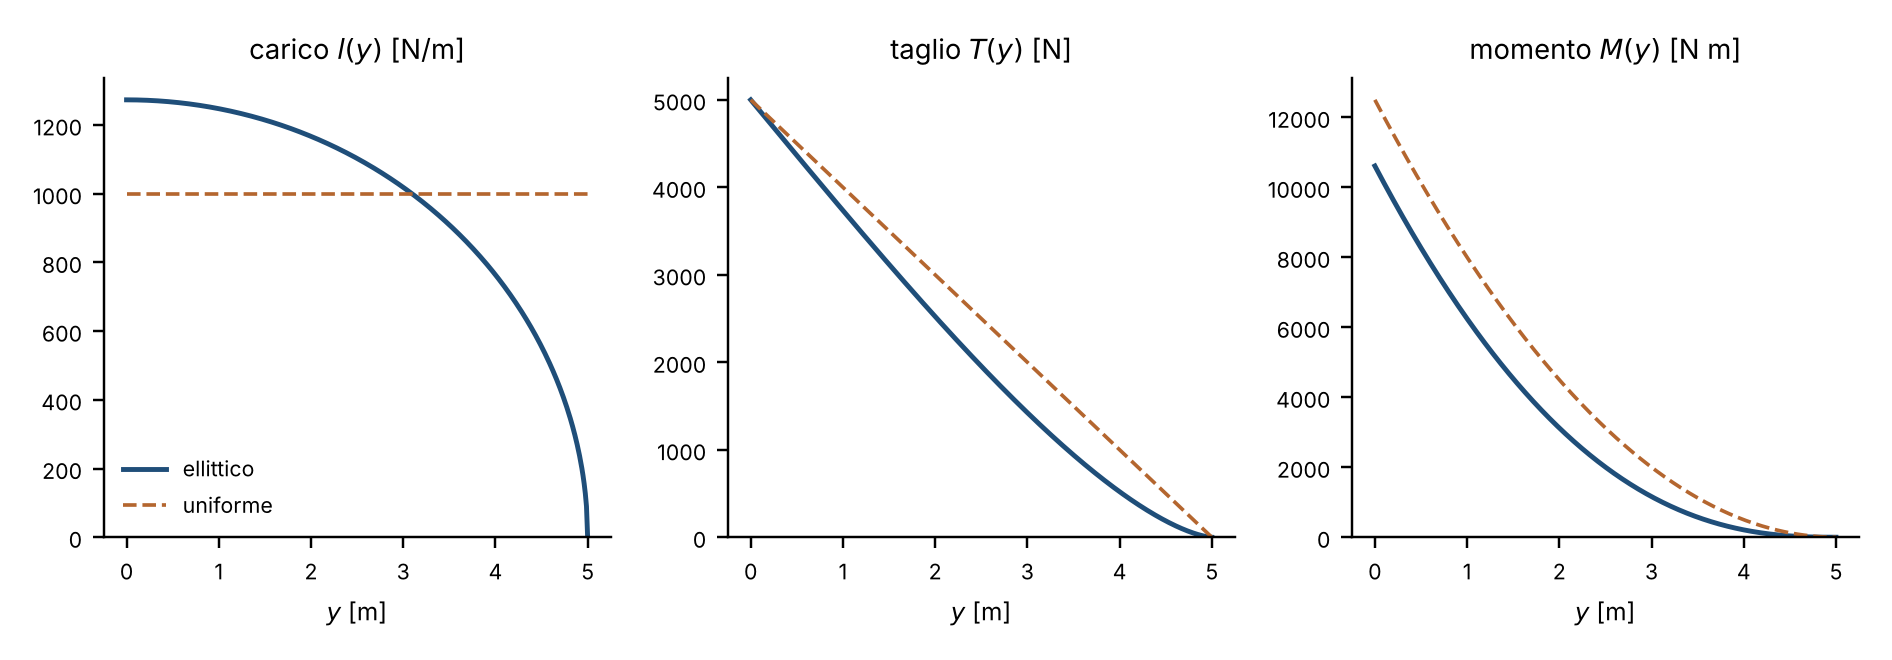
\includegraphics[width=\textwidth]{figure/taglio_momento.png}
\caption{Carico, taglio e momento flettente lungo la semiala per la distribuzione
ellittica ($W=10\,000$~N, $b=10$~m), confrontati con quelli di un carico uniforme con la
stessa portanza totale (tratteggio). Il taglio è l'area del carico all'esterno della
stazione, il momento l'area del taglio; le pendenze sono $T'=-l$ e $M'=-T$
(\texttt{python/fig\_taglio\_momento.py}).}
\label{fig:taglio-momento}
\end{figure}

Il programma seguente calcola il taglio e il momento numericamente, integrando il
carico dall'estremità verso la radice con la formula dei trapezi, e li confronta con le
formule \eqref{eq:taglio-ellittico} e \eqref{eq:momento-ellittico}.

\begin{python}[Taglio e momento flettente lungo la semiala]
import math

W, b = 10000.0, 10.0
s, l0 = b / 2, 4 * W / (math.pi * b)
l = lambda y: l0 * math.sqrt(max(0.0, 1 - (y / s)**2))

def T_esatto(y):
    u = y / s
    q = math.pi / 2 - math.asin(u) - u * math.sqrt(1 - u * u)
    return l0 * s / 2 * q

n = 5000                     # trapezi, dall'estremità alla radice
h = s / n
y = [s - k * h for k in range(n + 1)]
T, M = [0.0], [0.0]
for k in range(1, n + 1):
    T.append(T[-1] + h * (l(y[k - 1]) + l(y[k])) / 2)    # T' = -l
    M.append(M[-1] + h * (T[k - 1] + T[k]) / 2)          # M' = -T
print("  y [m]   T num. [N]  T esatto [N]   M num. [N m]")
for k in range(n, -1, -1000):
    print(f"{y[k]:6.1f}  {T[k]:10.1f}  {T_esatto(y[k]):11.1f}"
          f"  {M[k]:12.1f}")
print(f"M(0) esatto = W b/(3 pi) = {W * b / (3 * math.pi):.1f} N m")
\end{python}
\begin{risultato}
  y [m]   T num. [N]  T esatto [N]   M num. [N m]
   0.0      5000.0       5000.0       10610.3
   1.0      3735.3       3735.3        6244.8
   2.0      2523.2       2523.2        3122.3
   3.0      1423.8       1423.8        1161.1
   4.0       520.4        520.4         210.1
   5.0         0.0          0.0           0.0
M(0) esatto = W b/(3 pi) = 10610.3 N m
\end{risultato}

\begin{osservazione}[Un carico concentrato: il motore in ala]\label{oss:motore-ala}
Supponiamo che la semiala porti, oltre alla portanza $l$, il peso $P$ di un motore,
applicato nella stazione $y_{m}\in(0,s)$ e diretto verso il basso. Per $y<y_{m}$ il tratto
esterno $[y,s]$ comprende il motore, e le \eqref{eq:taglio-momento} diventano
\[
\begin{aligned}
  T(y)&=\int_{y}^{s}l(\eta)\,d\eta-P,\\
  M(y)&=\int_{y}^{s}(\eta-y)\,l(\eta)\,d\eta-P\,(y_{m}-y) \qquad (0\le y<y_{m}),
\end{aligned}
\]
mentre per $y\ge y_{m}$ restano invariate. Il taglio ha in $y_{m}$ un salto $P$; il
momento è continuo, ma ha in $y_{m}$ un punto angoloso, e $M'=-T$ vale soltanto per
$y\neq y_{m}$ (con la dimostrazione della \cref{prop:taglio-momento}). Dunque $M$ è
continua e regolare a tratti, e per il \cref{teo:formula-regolari-tratti}
$M(0)=-\int_{0}^{s}M'\,dy=\int_{0}^{s}T\,dy$: il momento alla radice è ancora l'area del
diagramma del taglio, mentre la stessa formula applicata al taglio, discontinuo,
sbaglierebbe di $P$ (\cref{oss:regolari-tratti-salti}). Si ha poi
$M(0)=\int_{0}^{s}y\,l(y)\,dy-P\,y_{m}$: il motore \emph{riduce} il momento alla radice, ed
è uno dei motivi per cui motori e combustibile si sistemano in ala. Con i dati
dell'\cref{es:taglio-ellittico}, $P=1000$~N e $y_{m}=1{,}5$~m, il momento scende da circa
$10\,610$ a circa $9\,110$~N\,m.
\end{osservazione}

\begin{notastorica}[Dalla trave di Galileo alle ali a sbalzo]
Il problema della resistenza di una trave incastrata a un estremo e caricata, la
\emph{mensola} o trave a sbalzo, fu posto da Galileo nei \emph{Discorsi e dimostrazioni
matematiche intorno a due nuove scienze} (1638), che lo risolse in modo errato quanto
alla distribuzione delle tensioni nella sezione. Le relazioni differenziali
$T'=-l$, $M'=-T$ e la teoria della flessione si consolidarono nel Settecento e
nell'Ottocento, con Jakob Bernoulli, Eulero e Navier. Tra le prime ali a sbalzo di impiego pratico, prive di
montanti e tiranti esterni, vi furono quelle realizzate da Hugo Junkers nel 1915 con il monoplano
metallico J~1: da allora il calcolo del taglio e del momento flettente lungo l'apertura,
cioè l'integrazione ripetuta della distribuzione di portanza, è il punto di partenza del
dimensionamento strutturale di ogni ala.
\end{notastorica}

%% ----------------------------------------------------------------------------
%%  §9.8  Appendice: integrali impropri
%% ----------------------------------------------------------------------------
\section{Appendice: integrali impropri}
\label{sec:impropri}

Nei paragrafi precedenti abbiamo studiato l'integrale definito di una funzione limitata
in un intervallo chiuso e limitato $[a,b]$. Nelle applicazioni è utile considerare anche
integrali come
\begin{equation}\label{eq:impropri-esempi}
  \int_{1}^{+\infty}\frac{dx}{x^{2}}, \qquad \int_{0}^{1}\frac{dx}{\sqrt x} .
\end{equation}
Tali integrali non rientrano nei casi trattati: nel primo l'intervallo di integrazione
è illimitato, nel secondo la funzione integranda non è limitata per $x\to0^{+}$. Integrali
di questo tipo si chiamano \emph{integrali impropri}.\index{integrale improprio} Come nel
testo di riferimento, ci limitiamo a funzioni \emph{continue} e \emph{non negative}
nell'intervallo considerato, e accenneremo al caso generale in un'osservazione.

\subsection{Intervalli illimitati}

Il punto di partenza è un fatto generale sulle funzioni monotòne, analogo al teorema
sulle successioni monotòne.

\begin{lemma}[Limite all'infinito di una funzione crescente]\label{lem:monotona-infinito}
Sia $F$ crescente in $[a,+\infty)$. Allora esiste il limite di $F(b)$ per $b\to+\infty$, ed è
uguale a $\sup\set{F(b) \tc b\ge a}$, finito se $F$ è limitata superiormente, $+\infty$ altrimenti.
\end{lemma}

\begin{schema}
\Ipotesi{$F$ crescente in $[a,+\infty)$.}
\Tesi{$\lim_{b\to+\infty}F(b)=\sup_{b\ge a}F(b)\in\R\cup\set{+\infty}$.}
\end{schema}

\begin{strategia}
È la stessa dimostrazione del teorema sulle successioni monotòne: un valore $F(b_{0})$
vicino all'estremo superiore si trova per la caratterizzazione dell'estremo superiore, e
la monotonia garantisce che tutti i valori successivi sono ancora più vicini.
\end{strategia}

\begin{dimostrazione}
Sia $\ell=\sup F$ finito e sia $\epsilon>0$. Per la \cref{prop:caratt-sup} esiste $b_{0}$ con
$F(b_{0})>\ell-\epsilon$; per $b>b_{0}$, la monotonia dà $\ell-\epsilon<F(b_{0})\le F(b)\le\ell$, cioè
$\abs{F(b)-\ell}<\epsilon$. Se invece $F$ non è limitata superiormente, per ogni $M$ esiste $b_{0}$
con $F(b_{0})>M$, e allora $F(b)>M$ per ogni $b>b_{0}$: $F(b)\to+\infty$.
\end{dimostrazione}

Sia ora $f$ continua e non negativa in $[a,+\infty)$, e sia $F(b)=\int_{a}^{b}f(x)\,dx$ per
$b\ge a$. Per l'additività e la positività dell'integrale, se $b_{1}<b_{2}$ si ha
$F(b_{2})-F(b_{1})=\int_{b_{1}}^{b_{2}}f\ge0$: $F$ è crescente (lo si vede anche dal teorema
fondamentale, perché $F'=f\ge0$). Per il lemma, esiste il limite di $F(b)$ per
$b\to+\infty$, ed è lecita la definizione seguente.

\begin{definizione}[Integrale improprio su un intervallo illimitato]
\label{def:improprio-illimitato}
Sia $f$ continua e non negativa in $[a,+\infty)$. Si pone
\begin{equation}\label{eq:improprio-illimitato}
  \int_{a}^{+\infty}f(x)\,dx=\lim_{b\to+\infty}\int_{a}^{b}f(x)\,dx .
\end{equation}
L'integrale improprio si dice \emph{convergente} se il limite è finito, \emph{divergente}
se il limite è $+\infty$.
\end{definizione}

In modo analogo si definisce l'integrale improprio di una funzione continua e non
negativa in $(-\infty,a]$, come limite per $b\to+\infty$ di $\int_{-b}^{a}f$, e in $(-\infty,+\infty)$,
come limite di $\int_{-b}^{b}f$. Per una funzione non negativa, quest'ultimo è convergente se e
solo se lo sono i due integrali su $(-\infty,0]$ e su $[0,+\infty)$, e ne è la somma.

\begin{esempio}[Gli integrali $\int_{1}^{+\infty}x^{-p}\,dx$]\label{es:impropri-p-infinito}
Per $p\neq1$, per la formula fondamentale,
\[
  \int_{1}^{b}\frac{dx}{x^{p}}=\Bigl[\frac{x^{1-p}}{1-p}\Bigr]_{1}^{b}=\frac{b^{1-p}}{1-p}+\frac1{p-1} ,
\]
e per $p=1$ si ha $\int_{1}^{b}\frac{dx}x=\log b$. Passando al limite per $b\to+\infty$,
\begin{equation}\label{eq:impropri-p-infinito}
  \int_{1}^{+\infty}\frac{dx}{x^{p}}=
  \begin{cases} \dfrac1{p-1} & \text{se } p>1,\\[4pt] +\infty & \text{se } p\le1 . \end{cases}
\end{equation}
In particolare $\int_{1}^{+\infty}\frac{dx}{x^{2}}=1$ (\cref{fig:impropri}, a sinistra): una regione
illimitata può avere area finita.
\end{esempio}

\begin{figure}[htb]
\centering
\begin{tikzpicture}
\begin{axis}[name=i1, width=0.52\textwidth, height=4.6cm, axis lines=middle,
  xmin=-0.2, xmax=8.4, ymin=-0.1, ymax=1.35, xtick={1,4,8}, ytick={1},
  title={\scriptsize $\int_{1}^{+\infty}x^{-2}dx=1$}, clip=false]
  \addplot[draw=none, fill=blu!22, domain=1:8.2, samples=80] {1/x^2} \closedcycle;
  \addplot[curva, domain=0.87:8.2, samples=80] {1/x^2};
  \addplot[curva2, dashed, domain=0.77:8.2, samples=80] {1/x};
  \node[font=\scriptsize, rame, anchor=south] at (axis cs:6.0,0.3) {$\frac1x$: area $+\infty$};
\end{axis}
\begin{axis}[at={(i1.east)}, anchor=west, xshift=0.7cm, width=0.46\textwidth,
  height=4.6cm, axis lines=middle, xmin=-0.1, xmax=1.25, ymin=-0.3, ymax=6.2,
  xtick={1}, ytick={1,5}, title={\scriptsize $\int_{0}^{1}x^{-1/2}dx=2$}]
  \addplot[draw=none, fill=blu!22, domain=0.026:1, samples=100] {1/sqrt(x)}
    \closedcycle;
  \addplot[curva, domain=0.026:1.2, samples=100] {1/sqrt(x)};
\end{axis}
\end{tikzpicture}
\caption{Due integrali impropri convergenti. A sinistra, la regione illimitata sotto
$\frac1{x^{2}}$ per $x\ge1$ ha area $1$, mentre quella sotto $\frac1x$ (tratteggio) ha area
infinita. A destra, la regione sotto $\frac1{\sqrt x}$ in $(0,1]$, illimitata verso l'alto, ha
area $2$.}
\label{fig:impropri}
\end{figure}

\begin{notastorica}[Il solido iperbolico acuto di Torricelli]
Che una figura illimitata possa avere misura finita fu una delle sorprese del Seicento.
Intorno al 1641 Evangelista Torricelli, che di lì a poco sarebbe succeduto a Galileo come
matematico del granduca di Toscana, studiò il solido generato dalla rotazione attorno
all'asse $x$ della regione sotto l'iperbole $y=\frac1x$, per $x\ge1$: un «corno»
infinitamente lungo, il \emph{solido iperbolico acuto}. Con gli indivisibili di Cavalieri
resi «curvi» (superfici cilindriche coassiali al posto delle sezioni piane) dimostrò che
il suo volume è uguale a quello di un cilindro finito, e pubblicò il risultato nel 1644,
nell'\emph{Opera geometrica}, con una seconda dimostrazione alla maniera di Archimede per
i lettori diffidenti verso gli indivisibili. In termini moderni, le sezioni
perpendicolari all'asse sono cerchi di area $\frac\pi{x^{2}}$, e il volume è
$\pi\int_{1}^{+\infty}\frac{dx}{x^{2}}=\pi$ per la \eqref{eq:impropri-p-infinito}, mentre la
superficie laterale è infinita, come lascia intuire il confronto con $\int_{1}^{+\infty}\frac{dx}x$.
Il risultato alimentò a lungo le discussioni filosofiche sull'infinito, come la polemica
tra Thomas Hobbes e John Wallis.
\end{notastorica}

Non sempre è possibile calcolare esplicitamente una primitiva. In tal caso può essere
utile il criterio seguente.

\begin{teorema}[Criterio del confronto]\label{teo:confronto-impropri}
\index{criterio!del confronto per gli integrali impropri}
Siano $f$ e $g$ continue in $[a,+\infty)$, con $0\le f(x)\le g(x)$ per ogni $x\ge a$. Se
l'integrale improprio di $g$ in $[a,+\infty)$ è convergente, anche quello di $f$ è
convergente, e $\int_{a}^{+\infty}f\le\int_{a}^{+\infty}g$. Se l'integrale di $f$ è divergente, anche
quello di $g$ è divergente.
\end{teorema}

\needspace{6\baselineskip}
\begin{schema}
\Ipotesi{$f$, $g$ continue in $[a,+\infty)$; \ $0\le f\le g$.}
\Tesi{$\int_{a}^{+\infty}g<+\infty\implica\int_{a}^{+\infty}f<+\infty$;\\
$\int_{a}^{+\infty}f=+\infty\implica\int_{a}^{+\infty}g=+\infty$.}
\end{schema}

\begin{strategia}
Il confronto vale per gli integrali su $[a,b]$, per ogni $b$; i due membri hanno limite per
$b\to+\infty$, e il confronto passa ai limiti.
\end{strategia}

\begin{dimostrazione}
Per il \cref{teo:confronto-integrali}, $\int_{a}^{b}f\le\int_{a}^{b}g$ per ogni $b>a$. Entrambi i membri
hanno limite per $b\to+\infty$; per il confronto dei limiti (\cref{teo:confronto-funzioni}),
il limite del primo membro non supera quello del secondo. Se il secondo è finito, lo è
anche il primo; se il primo è $+\infty$, lo è anche il secondo.
\end{dimostrazione}

\begin{esempio}[L'integrale di Gauss converge]\label{es:gauss-converge}
Verifichiamo che $\int_{0}^{+\infty}e^{-x^{2}}dx<+\infty$. L'integrale converge se e solo se converge
quello su $[1,+\infty)$, perché i due differiscono per l'integrale (finito) su $[0,1]$. Per
$x\ge1$ si ha $1\le x$ e, moltiplicando per $e^{-x^{2}}>0$,
\[
  e^{-x^{2}}\le x\,e^{-x^{2}} \qquad\perogni x\ge1 .
\]
La funzione a destra ha il vantaggio di avere una primitiva facilmente calcolabile, per
la \eqref{eq:integrali-composti}:
\[
  \int_{1}^{+\infty}x\,e^{-x^{2}}dx=\lim_{b\to+\infty}\Bigl[-\frac12e^{-x^{2}}\Bigr]_{1}^{b}
  =\lim_{b\to+\infty}\Bigl(\frac1{2e}-\frac12e^{-b^{2}}\Bigr)=\frac1{2e} .
\]
Per il criterio del confronto, l'integrale di $e^{-x^{2}}$ converge. Il suo valore,
$\int_{0}^{+\infty}e^{-x^{2}}dx=\frac{\sqrt\pi}2$, si calcola con gli integrali doppi (in un corso di Analisi
Matematica~2); qui lo verifichiamo numericamente. La convergenza appena dimostrata,
insieme alla parità di $e^{-x^{2}}$, giustifica gli asintoti orizzontali della funzione
integrale nella \cref{fig:funzione-integrale}: $F(x)=\int_{0}^{x}e^{-t^{2}}dt$ è crescente e
tende a un limite finito per $x\to+\infty$, e $F(-x)=-F(x)$.
\end{esempio}

\begin{esempio}[La velocità di fuga]\label{es:velocita-fuga}
Il lavoro necessario per vincere la forza di gravità $F(r)=\frac{GMm}{r^{2}}$ (l'opposto del
lavoro della forza peso) quando una massa $m$ si allontana dalla superficie terrestre
($r=R$) fino a una distanza $r_{1}$ è, come limite delle somme
$\sum F(r_{k})\,\Delta r_{k}$, l'integrale $\int_{R}^{r_{1}}\frac{GMm}{r^{2}}\,dr=GMm\bigl(\frac1R-\frac1{r_{1}}\bigr)$. Per
$r_{1}\to+\infty$ si ottiene l'integrale improprio convergente
\[
  \int_{R}^{+\infty}\frac{GMm}{r^{2}}\,dr=\frac{GMm}R=m\,g\,R ,
\]
dove $g=\frac{GM}{R^{2}}$ è l'accelerazione di gravità al suolo. Un corpo lanciato con velocità
$v$ sfugge all'attrazione terrestre (trascurando l'atmosfera) se la sua energia cinetica
$\frac12mv^{2}$ basta a compiere questo lavoro, cioè se $v\ge\sqrt{2gR}$: con $g=9{,}81$~m/s$^{2}$ e
$R=6371$~km si ottiene la velocità di fuga $\sqrt{2gR}\approx11{,}2$~km/s. Che il lavoro
per portare un corpo «all'infinito» sia finito dipende dal fatto che la forza decresce
come $r^{-2}$, cioè con esponente $p=2>1$ nella \eqref{eq:impropri-p-infinito}.
\end{esempio}

\subsection{Funzioni non limitate}

In modo analogo si procede per una funzione non limitata in prossimità di un estremo
dell'intervallo di integrazione, ad esempio dell'estremo $a$. Sia $f$ continua e non
negativa in $(a,b]$; per $0<h<b-a$ la funzione $h\mapsto\int_{a+h}^{b}f$ è decrescente (al crescere
di $h$ l'intervallo si restringe e la funzione integranda è non negativa), e quindi
esiste il limite per $h\to0^{+}$ (con la stessa dimostrazione del
\cref{lem:monotona-infinito}). Si pone
\begin{equation}\label{eq:improprio-non-limitata}
  \int_{a}^{b}f(x)\,dx=\lim_{h\to0^{+}}\int_{a+h}^{b}f(x)\,dx ,
\end{equation}
e l'integrale improprio si dice convergente se il limite è finito, divergente
altrimenti. Vale un criterio del confronto del tutto analogo al
\cref{teo:confronto-impropri}, con la stessa dimostrazione.

\begin{esempio}[Gli integrali $\int_{0}^{1}x^{-p}\,dx$]\label{es:impropri-p-zero}
Per $p\neq1$, $\int_{h}^{1}x^{-p}\,dx=\frac1{1-p}-\frac{h^{1-p}}{1-p}$, e per $p=1$ si ha
$\int_{h}^{1}\frac{dx}x=-\log h$. Passando al limite per $h\to0^{+}$,
\begin{equation}\label{eq:impropri-p-zero}
  \int_{0}^{1}\frac{dx}{x^{p}}=
  \begin{cases} \dfrac1{1-p} & \text{se } p<1,\\[4pt] +\infty & \text{se } p\ge1 . \end{cases}
\end{equation}
In particolare $\int_{0}^{1}\frac{dx}{\sqrt x}=2$ (\cref{fig:impropri}, a destra). Si noti che i ruoli di
$p>1$ e $p<1$ sono scambiati rispetto alla \eqref{eq:impropri-p-infinito}: all'infinito
conviene che la funzione decresca rapidamente, vicino a $0$ che cresca lentamente. Il
tempo di salita alla quota di tangenza teorica dell'\cref{es:tempo-salita},
$\int_{0}^{H}\frac{d\eta}{v_{z0}(1-\eta/H)}$, è un integrale di questo tipo nell'estremo $H$ (con
$p=1$, dopo la sostituzione $\eta=H-x$), e quindi diverge.
\end{esempio}

\begin{osservazione}[Funzioni di segno qualsiasi]\label{oss:convergenza-assoluta}
Se $f$ è continua in $[a,+\infty)$ ma cambia segno, la funzione $\int_{a}^{b}f$ non è più
monotòna e il suo limite può non esistere. Se però $\int_{a}^{+\infty}\abs f$ converge, si dice che
l'integrale di $f$ è \emph{assolutamente convergente}, e il limite
$\lim_{b\to+\infty}\int_{a}^{b}f$ esiste finito. Infatti le parti positiva e negativa
\eqref{eq:parte-positiva-negativa} verificano $0\le f^{\pm}\le\abs f$ e sono continue; per il
criterio del confronto i loro integrali convergono, e
$\int_{a}^{b}f=\int_{a}^{b}f^{+}-\int_{a}^{b}f^{-}$ tende alla differenza dei due limiti. Ad esempio,
$\int_{1}^{+\infty}\frac{\sen x}{x^{2}}\,dx$ converge assolutamente, perché
$\bigl|\frac{\sen x}{x^{2}}\bigr|\le\frac1{x^{2}}$. Esistono anche integrali convergenti ma non
assolutamente convergenti, come $\int_{0}^{+\infty}\frac{\sen x}x\,dx$, che studieremo nel
\S\ref{subsec:seno-su-x}.
\end{osservazione}

\begin{python}[Integrali impropri: verifiche numeriche]
import math

def punto_medio(f, a, b, n=200000):
    h = (b - a) / n
    return h * sum(f(a + (k + 0.5) * h) for k in range(n))

for B in (1, 2, 4, 6):
    I = punto_medio(lambda x: math.exp(-x * x), 0, B)
    print(f"int_0^{B} exp(-x^2) dx = {I:.10f}")
print(f"sqrt(pi)/2           = {math.sqrt(math.pi) / 2:.10f}")
for p in (0.5, 1, 2):
    v = [punto_medio(lambda x: x**-p, 1, B, 20000)
         for B in (10, 100, 1000)]
    print(f"p = {p}: int_1^B x^-p dx (B = 10, 100, 1000) =",
          ", ".join(f"{w:.3f}" for w in v))
g, R = 9.81, 6.371e6
print(f"velocità di fuga = {math.sqrt(2 * g * R) / 1000:.2f} km/s")
\end{python}
\begin{risultato}
int_0^1 exp(-x^2) dx = 0.7468241328
int_0^2 exp(-x^2) dx = 0.8820813908
int_0^4 exp(-x^2) dx = 0.8862269118
int_0^6 exp(-x^2) dx = 0.8862269255
sqrt(pi)/2           = 0.8862269255
p = 0.5: int_1^B x^-p dx (B = 10, 100, 1000) = 4.325, 18.000, 61.246
p = 1: int_1^B x^-p dx (B = 10, 100, 1000) = 2.303, 4.605, 6.908
p = 2: int_1^B x^-p dx (B = 10, 100, 1000) = 0.900, 0.990, 0.999
velocità di fuga = 11.18 km/s
\end{risultato}

\begin{notastorica}[L'integrale di Gauss]
L'integrale $\int_{-\infty}^{+\infty}e^{-x^{2}}dx=\sqrt\pi$ comparve per la prima volta nei lavori di Abraham
de Moivre (1733) sull'approssimazione della distribuzione binomiale, e il suo valore fu
poi stabilito da Laplace e da Gauss, che lo usò nel 1809 nella teoria degli errori di
misura legata al metodo dei minimi quadrati (\cref{sec:estremi-due}). Per questo la
funzione $e^{-x^{2}}$, opportunamente normalizzata, si chiama «gaussiana». Gli integrali
impropri, definiti come limiti di integrali ordinari, furono trattati sistematicamente
da Cauchy nelle lezioni del 1823.
\end{notastorica}

\subsection{Approfondimento: un integrale convergente ma non assolutamente convergente}
\label{subsec:seno-su-x}

Se $f$ è continua in $[a,+\infty)$ e ha segno qualsiasi, diciamo che l'integrale improprio
$\int_{a}^{+\infty}f(x)\,dx$ è \emph{convergente} se esiste finito il limite di $\int_{a}^{b}f$
per $b\to+\infty$, e indichiamo il limite con lo stesso simbolo. Per l'\cref{oss:convergenza-assoluta},
un integrale assolutamente convergente è convergente; il viceversa è falso, e l'esempio
classico è quello di $\frac{\sen x}x$, che, seguendo \cite{giusti}, possiamo studiare con i
soli strumenti di questo capitolo. Ci limitiamo all'intervallo $[1,+\infty)$: in $[0,1]$
la funzione $\frac{\sen x}x$, prolungata con il valore $1$ in $x=0$ (per il limite notevole
\eqref{eq:lim-senx-x}), è continua, e il suo integrale è un integrale ordinario.

\begin{proposizione}[L'integrale di $\frac{\sen x}x$]\label{prop:seno-su-x}
L'integrale improprio $\int_{1}^{+\infty}\frac{\sen x}x\,dx$ è convergente, ma non
assolutamente convergente: $\int_{1}^{+\infty}\frac{\abs{\sen x}}x\,dx=+\infty$.
\end{proposizione}

\begin{schema}
\Ipotesi{$f(x)=\frac{\sen x}x$, continua in $[1,+\infty)$.}
\Tesi{$\lim_{b\to+\infty}\int_{1}^{b}f$ esiste finito; \ $\int_{1}^{+\infty}\abs f=+\infty$.}
\end{schema}

\begin{strategia}
$\frac{\sen x}x$ decresce soltanto come $\frac1x$, che da solo non basterebbe; ma le
oscillazioni del seno producono compensazioni, che un'integrazione per parti rende
visibili, trasformando l'integrale in uno con $\frac{\cos x}{x^{2}}$, assolutamente
convergente. Per $\int\abs f$ si stima dal basso l'integrale su ogni arco
$[k\pi,(k+1)\pi]$ e si confronta la somma delle stime con $\int\frac{dt}t$, che diverge.
\end{strategia}

\begin{dimostrazione}
Per $b>1$, integrando per parti (\cref{teo:per-parti-definito}) con fattore finito
$\frac1x$ e fattore differenziale $\sen x$,
\begin{equation}\label{eq:seno-su-x-parti}
\begin{split}
  \int_{1}^{b}\frac{\sen x}x\,dx&=\Bigl[-\frac{\cos x}x\Bigr]_{1}^{b}
  -\int_{1}^{b}\frac{\cos x}{x^{2}}\,dx\\
  &=\cos1-\frac{\cos b}b-\int_{1}^{b}\frac{\cos x}{x^{2}}\,dx .
\end{split}
\end{equation}
Per $b\to+\infty$, $\frac{\cos b}b\to0$, perché $\abs{\cos b}\le1$; l'ultimo integrale ha limite
finito, perché $\bigl|\frac{\cos x}{x^{2}}\bigr|\le\frac1{x^{2}}$ e quindi converge assolutamente
(\cref{oss:convergenza-assoluta} e \eqref{eq:impropri-p-infinito} con $p=2$). Dunque il primo
membro ha limite finito.

Per la seconda affermazione, sia $k\in\N$. Con la sostituzione $x=u+k\pi$, poiché
$\abs{\sen(u+k\pi)}=\sen u$ per $u\in[0,\pi]$, si ha
$\int_{k\pi}^{(k+1)\pi}\abs{\sen x}\,dx=\int_{0}^{\pi}\sen u\,du=2$; inoltre
$\frac1x\ge\frac1{(k+1)\pi}$ per $x\le(k+1)\pi$. Per il confronto,
\[
  \int_{k\pi}^{(k+1)\pi}\frac{\abs{\sen x}}x\,dx\ge\frac2{(k+1)\pi}
  \ge\frac2\pi\int_{k+1}^{k+2}\frac{dt}t ,
\]
perché $\frac1t\le\frac1{k+1}$ in $[k+1,k+2]$. Sommando per $k=1,\dots,n$ e usando l'additività,
\[
  \int_{1}^{(n+1)\pi}\frac{\abs{\sen x}}x\,dx\ge\int_{\pi}^{(n+1)\pi}\frac{\abs{\sen x}}x\,dx
  \ge\frac2\pi\int_{2}^{n+2}\frac{dt}t=\frac2\pi\log\frac{n+2}2 ,
\]
che tende a $+\infty$. La funzione crescente $b\mapsto\int_{1}^{b}\frac{\abs{\sen x}}x\,dx$ non è
dunque limitata, e per il \cref{lem:monotona-infinito} tende a $+\infty$.
\end{dimostrazione}

Le compensazioni tra archi positivi e negativi sono decisive, come nelle serie a segni
alterni del \cref{cap:serie}. Il valore $\int_{0}^{+\infty}\frac{\sen x}x\,dx=\frac\pi2$ si
calcola in Analisi Matematica~2; il programma seguente lo verifica numericamente, con la
crescita logaritmica di $\int_{0}^{B}\frac{\abs{\sen x}}x\,dx$ prevista dalla dimostrazione.

\begin{python}[Convergenza semplice e divergenza assoluta]
import math

def punto_medio(f, a, b, n):
    h = (b - a) / n
    return h * sum(f(a + (k + 0.5) * h) for k in range(n))

f = lambda x: math.sin(x) / x
g = lambda x: abs(math.sin(x)) / x
print("    B   int_0^B sen x/x   int_0^B |sen x|/x   (2/pi) log B")
for B in (10, 100, 1000, 10000):
    I = punto_medio(f, 0, B, 100 * B)
    J = punto_medio(g, 0, B, 100 * B)
    L = 2 / math.pi * math.log(B)
    print(f"{B:5d}   {I:15.6f}   {J:17.6f}   {L:12.6f}")
print(f"pi/2 = {math.pi / 2:.6f}")
\end{python}
\begin{risultato}
    B   int_0^B sen x/x   int_0^B |sen x|/x   (2/pi) log B
   10          1.658348            2.558747       1.465871
  100          1.562225            4.046675       2.931742
 1000          1.570233            5.510356       4.397614
10000          1.570892            6.976394       5.863485
pi/2 = 1.570796
\end{risultato}

La prima colonna si stabilizza su $\frac\pi2$; la seconda differisce dall'ultima per circa
$1{,}11$: l'integrale di $\frac{\abs{\sen x}}x$ cresce come $\frac2\pi\log B$.

%% ----------------------------------------------------------------------------
%%  §9.9  Appendice: definizione di logaritmo, esponenziale, potenza
%% ----------------------------------------------------------------------------
\section{Appendice: logaritmo, esponenziale e potenza mediante un integrale}
\label{sec:logaritmo-integrale}

Nel \cref{cap:numeri} abbiamo introdotto le funzioni potenza, esponenziale e logaritmo a
partire dall'espressione $a^{b}$, appoggiandoci inizialmente all'idea intuitiva di
elevamento a potenza con esponente reale; nel \cref{cap:complementi} abbiamo dato un
significato rigoroso ad $a^{b}$ mediante l'estremo superiore. In questo paragrafo seguiamo
una strada diversa, basata sull'integrale definito: \emph{definiamo} il logaritmo come
una funzione integrale, e da esso deduciamo l'esponenziale e la potenza. Supponiamo
validi gli assiomi dei numeri reali, con il prodotto, il quoziente e le potenze $a^{n}$
con esponente naturale, e utilizziamo soltanto risultati dimostrati senza far uso delle
tre funzioni che vogliamo definire: in particolare, il numero $e$ definito come limite
della successione $\bigl(1+\frac1n\bigr)^{n}$ (\cref{teo:numero-e}), il teorema fondamentale, la
formula di sostituzione con una funzione lineare e i teoremi sulle funzioni monotòne e
sulle funzioni inverse.

La funzione $\frac1t$ è continua e decrescente per $t>0$. Poniamo, per $x>0$,
\begin{equation}\label{eq:L-definizione}
  L(x)=\int_{1}^{x}\frac{dt}t \qquad (x>0) .
\end{equation}
Per $x>1$, $L(x)$ è l'area sotto l'iperbole $y=\frac1t$ tra $1$ e $x$; per $0<x<1$ è l'opposto
dell'area tra $x$ e $1$ (\cref{fig:logaritmo-area}).

\begin{proposizione}[Proprietà della funzione $L$]\label{prop:L-proprieta}
La funzione $L$ definita dalla \eqref{eq:L-definizione} ha le proprietà seguenti.
\begin{enumerate}[label=\textup{(\alph*)}]
  \item $L$ è derivabile in $(0,+\infty)$ con $L'(x)=\frac1x$; è quindi continua e strettamente
  crescente, e $L(1)=0$.
  \item $L(x_{1}x_{2})=L(x_{1})+L(x_{2})$ per ogni $x_{1},x_{2}>0$; in particolare
  $L(x^{n})=n\,L(x)$ per ogni $n\in\N$ e $L\bigl(\frac1x\bigr)=-L(x)$.
  \item $L(e)=1$.
  \item $L$ è una biiezione di $(0,+\infty)$ su $\R$.
\end{enumerate}
\end{proposizione}

\needspace{9\baselineskip}
\begin{schema}
\Ipotesi{$L(x)=\int_{1}^{x}\frac{dt}t$ per $x>0$; \ $e=\lim\bigl(1+\frac1n\bigr)^{n}$.}
\Tesi{(a) $L'=\frac1x$, $L$ strettamente crescente, $L(1)=0$; \ (b) $L(x_{1}x_{2})=L(x_{1})+L(x_{2})$;
\ (c) $L(e)=1$; \ (d) $L:(0,+\infty)\to\R$ biiettiva.}
\end{schema}

\begin{strategia}
(a) è il teorema fondamentale. (b) è il cuore della questione: l'area sotto l'iperbole tra
$x_{1}$ e $x_{1}x_{2}$ è uguale a quella tra $1$ e $x_{2}$, perché la sostituzione $t=x_{1}s$ allarga
le basi di un fattore $x_{1}$ e riduce le altezze dello stesso fattore. (c) si ottiene
riconoscendo in $L\bigl((1+\frac1n)^{n}\bigr)=n\,L(1+\frac1n)$ un rapporto incrementale di $L$ in $1$. Per (d),
la (b) mostra che $L$ non è limitata né superiormente né inferiormente, e il teorema dei
valori intermedi fa il resto.
\end{strategia}

\begin{dimostrazione}
(a) Per il \cref{teo:fondamentale} (applicato in un intervallo chiuso contenuto in
$(0,+\infty)$ che contenga $1$ e abbia $x$ al suo interno), $L$ è derivabile con
$L'(x)=\frac1x>0$; per il
\cref{cor:derivata-positiva} è strettamente crescente, ed è continua perché derivabile.
Inoltre $L(1)=\int_{1}^{1}=0$.

(b) Fissati $x_{1},x_{2}>0$, per l'additività
\[
  L(x_{1}x_{2})=\int_{1}^{x_{1}x_{2}}\frac{dt}t=\int_{1}^{x_{1}}\frac{dt}t+\int_{x_{1}}^{x_{1}x_{2}}\frac{dt}t .
\]
Nell'ultimo integrale effettuiamo la sostituzione $t=g(s)=x_{1}s$, con $g'(s)=x_{1}$,
$g(1)=x_{1}$ e $g(x_{2})=x_{1}x_{2}$; per il \cref{teo:sostituzione-definita},
\[
  \int_{x_{1}}^{x_{1}x_{2}}\frac{dt}t=\int_{1}^{x_{2}}\frac{x_{1}\,ds}{x_{1}s}=\int_{1}^{x_{2}}\frac{ds}s=L(x_{2}) ,
\]
(se $x_{2}<1$ gli estremi sono in ordine decrescente, e le formule valgono per la
\eqref{eq:estremi-invertiti}), e quindi $L(x_{1}x_{2})=L(x_{1})+L(x_{2})$. Per induzione su $n$ si ottiene $L(x^{n})=nL(x)$; con
$x_{1}=x$, $x_{2}=\frac1x$ si ottiene $0=L(1)=L(x)+L\bigl(\frac1x\bigr)$.

(c) Sia $x_{n}=\bigl(1+\frac1n\bigr)^{n}$. Per la (b) e poiché $L(1)=0$,
\[
  L(x_{n})=n\,L\Bigl(1+\frac1n\Bigr)=\frac{L(1+\frac1n)-L(1)}{\frac1n} ,
\]
che è il rapporto incrementale di $L$ nel punto $1$ con incremento $\frac1n$; per la (a) esso
tende a $L'(1)=1$ (lungo la successione $h=\frac1n$, per la definizione stessa di limite di una
funzione, \cref{def:limite-funzione}). D'altra parte $x_{n}\to e$ e $L$ è continua, quindi $L(x_{n})\to L(e)$ (per la
\cref{prop:caratt-continuita}). Per l'unicità del limite, $L(e)=1$.

(d) Per la (a), $L$ è iniettiva. Poiché $L(2)>L(1)=0$, per la (b) si ha $L(2^{n})=nL(2)\to+\infty$
e $L(2^{-n})=-nL(2)\to-\infty$. Dato $y\in\R$, esistono quindi $n\in\N$ con $L(2^{-n})<y<L(2^{n})$, e
per il teorema dei valori intermedi (\cref{teo:valori-intermedi-2}), applicato alla funzione
continua $L$ nell'intervallo $[2^{-n},2^{n}]$, esiste $x$ con $L(x)=y$: $L$ è suriettiva su $\R$.
\end{dimostrazione}

\begin{figure}[htb]
\centering
\begin{tikzpicture}
\begin{axis}[name=g1, width=0.5\textwidth, height=4.6cm, axis lines=middle,
  xmin=-0.1, xmax=4.4, ymin=-0.1, ymax=2.3, xtick={1,3}, xticklabels={$1$,$x$},
  ytick={1}, title={\scriptsize $L(x)=\int_{1}^{x}\frac{dt}t$}]
  \addplot[draw=none, fill=blu!22, domain=1:3, samples=50] {1/x} \closedcycle;
  \addplot[curva, domain=0.45:4.3, samples=100] {1/x};
  \node[font=\scriptsize, blu] at (axis cs:1.9,0.22) {$L(x)$};
\end{axis}
\begin{axis}[at={(g1.east)}, anchor=west, xshift=0.7cm, width=0.5\textwidth,
  height=4.6cm, axis lines=middle, xmin=-0.1, xmax=4.4, ymin=-0.1, ymax=1.3,
  xtick={1,1.5,2.5,3.75}, xticklabels={$1$,$x_{2}$,$x_{1}$,$x_{1}x_{2}$},
  ytick=\empty, title={\scriptsize aree uguali: $L(x_{1}x_{2})-L(x_{1})=L(x_{2})$},
  tick label style={font=\scriptsize}]
  \addplot[draw=none, fill=blu!22, domain=1:1.5, samples=40] {1/x} \closedcycle;
  \addplot[draw=none, fill=rame!30, domain=2.5:3.75, samples=40] {1/x} \closedcycle;
  \addplot[curva, domain=0.8:4.3, samples=100] {1/x};
\end{axis}
\end{tikzpicture}
\caption{A sinistra, il logaritmo come area sotto l'iperbole. A destra, la regione tra
$1$ e $x_{2}$ e quella tra $x_{1}$ e $x_{1}x_{2}$ (qui $x_{1}=2{,}5$, $x_{2}=1{,}5$) hanno la stessa area: la
seconda si ottiene dalla prima allargando le basi di un fattore $x_{1}$ e riducendo le
altezze dello stesso fattore. È la proprietà $L(x_{1}x_{2})=L(x_{1})+L(x_{2})$.}
\label{fig:logaritmo-area}
\end{figure}

Per la \cref{prop:L-proprieta}(d), la funzione $L$ è invertibile. Indichiamo con
$E:\R\to(0,+\infty)$ la funzione inversa, definita da
\begin{equation}\label{eq:E-definizione}
  E(y)=x \quad\sse\quad L(x)=y .
\end{equation}

\needspace{9\baselineskip}
\begin{proposizione}[Proprietà della funzione $E$]\label{prop:E-proprieta}
La funzione $E$ è continua, strettamente crescente e derivabile in $\R$, con
\begin{equation}\label{eq:E-proprieta}
\begin{gathered}
  E'(y)=E(y), \qquad E(0)=1, \qquad E(1)=e,\\
  E(y_{1}+y_{2})=E(y_{1})\,E(y_{2}) .
\end{gathered}
\end{equation}
Inoltre, per ogni $a>0$ e $n\in\N$, $E\bigl(n\,L(a)\bigr)=a^{n}$.
\end{proposizione}

\begin{schema}
\Ipotesi{$E=L^{-1}:\R\to(0,+\infty)$.}
\Tesi{$E$ continua, strettamente crescente, $E'=E$; \ $E(0)=1$, $E(1)=e$;
\ $E(y_{1}+y_{2})=E(y_{1})E(y_{2})$; \ $E(nL(a))=a^{n}$.}
\end{schema}

\begin{strategia}
Le proprietà di regolarità passano dalla funzione alla sua inversa per i teoremi sulle
funzioni inverse. Le identità algebriche si ottengono applicando $L$, che è iniettiva, a
entrambi i membri e usando la \cref{prop:L-proprieta}.
\end{strategia}

\begin{dimostrazione}
In ogni intervallo chiuso $[\alpha,\beta]\subset(0,+\infty)$ la funzione $L$ è continua e strettamente
crescente; per i \cref{teo:continuita-inversa,teo:derivata-inversa} la sua inversa è
continua e strettamente crescente in $[L(\alpha),L(\beta)]$, e derivabile con
$E'(y)=\frac1{L'(E(y))}=E(y)$. Poiché ogni $y\in\R$ è interno a un intervallo di questo tipo,
le proprietà valgono in tutto $\R$. Da $L(1)=0$ e $L(e)=1$ seguono $E(0)=1$ ed $E(1)=e$. Posto
$x_{i}=E(y_{i})$, per la \cref{prop:L-proprieta}(b) $L(x_{1}x_{2})=y_{1}+y_{2}$, cioè
$E(y_{1}+y_{2})=x_{1}x_{2}=E(y_{1})E(y_{2})$. Infine $L(a^{n})=nL(a)$, cioè $E(nL(a))=a^{n}$.
\end{dimostrazione}

L'identità $a^{n}=E\bigl(n\,L(a)\bigr)$ esprime la potenza a esponente naturale mediante
$E$ e $L$, e suggerisce come definire la potenza con esponente reale.

\begin{definizione}[Potenza con esponente reale]\label{def:potenza-integrale}
Se $a$ e $x$ sono numeri reali, con $a>0$, si pone
\begin{equation}\label{eq:potenza-integrale}
  a^{x}=E\bigl(x\,L(a)\bigr) .
\end{equation}
\end{definizione}

La definizione è coerente con quella elementare: per $x=n\in\N$ restituisce $a^{n}$ (per la
\cref{prop:E-proprieta}); per $x=\frac mn$, con $m,n\in\N$, il numero $a^{m/n}$ così definito è
positivo e verifica, per la \eqref{eq:E-proprieta},
$\bigl(a^{m/n}\bigr)^{n}=E\bigl(\frac mnL(a)\bigr)^{n}=E\bigl(mL(a)\bigr)=a^{m}$, cioè è la radice $n$-esima
positiva di $a^{m}$, come nella \eqref{eq:potenza-razionale}. Inoltre $E(0)=1=a^{0}$ e,
poiché $E(y)\,E(-y)=E(0)=1$, si ha $a^{-m/n}=E\bigl(-\frac mnL(a)\bigr)=\frac1{a^{m/n}}$, ancora in
accordo con la \eqref{eq:potenza-razionale}. Le due funzioni $x\mapsto E(xL(a))$ e $x\mapsto a^{x}$
(quella del \cref{cap:complementi}, continua per il \cref{teo:continuita-esponenziale})
sono continue in $\R$ e coincidono sui razionali; poiché ogni numero reale $x$ è limite di
una successione di razionali (basta scegliere $q_{k}\in\Q\cap(x-\frac1k,x)$, che esiste per il
\cref{teo:densita-Q}), per la \cref{prop:caratt-continuita} esse coincidono ovunque. In particolare, per $a=e$,
poiché $L(e)=1$, si ha la \emph{funzione esponenziale}
\begin{equation}\label{eq:esponenziale-integrale}
  e^{x}=E(x) ,
\end{equation}
e, poiché il logaritmo naturale è la funzione inversa di $e^{x}$,
\begin{equation}\label{eq:logaritmo-integrale}
  \log x=L(x)=\int_{1}^{x}\frac{dt}t \qquad (x>0) .
\end{equation}
Risultano così definite le funzioni potenza, esponenziale e logaritmo, e si riconosce
facilmente che esse godono delle proprietà illustrate nel \cref{cap:numeri}. Ad esempio,
$\log(x_{1}x_{2})=\log x_{1}+\log x_{2}$ è la \cref{prop:L-proprieta}(b), che applicata a
$\frac{x_{1}}{x_{2}}$ e $x_{2}$ dà $\log\frac{x_{1}}{x_{2}}=\log x_{1}-\log x_{2}$.

\begin{python}[Il logaritmo come area e l'esponenziale come sua inversa]
import math

def L(x, n=100000):
    """L(x) = int_1^x dt/t, formula del punto medio."""
    h = (x - 1) / n
    return h * sum(1 / (1 + (k + 0.5) * h) for k in range(n))

def E(y):
    """Inversa di L, per bisezione (L è crescente)."""
    a, b = 1e-6, 1e6
    for _ in range(80):
        m = math.sqrt(a * b)            # bisezione «geometrica»
        a, b = (m, b) if L(m, 2000) < y else (a, m)
    return math.sqrt(a * b)

for x in (0.5, 2, 3, 6, math.e):
    print(f"L({x:.4f}) = {L(x):.8f}   log = {math.log(x):.8f}")
print(f"L(2) + L(3) = {L(2) + L(3):.8f} = L(6)")
for y in (-1, 1, 2):
    print(f"E({y:2d}) = {E(y):.5f}   exp = {math.exp(y):.5f}")
\end{python}
\begin{risultato}
L(0.5000) = -0.69314718   log = -0.69314718
L(2.0000) = 0.69314718   log = 0.69314718
L(3.0000) = 1.09861229   log = 1.09861229
L(6.0000) = 1.79175947   log = 1.79175947
L(2.7183) = 1.00000000   log = 1.00000000
L(2) + L(3) = 1.79175947 = L(6)
E(-1) = 0.36788   exp = 0.36788
E( 1) = 2.71828   exp = 2.71828
E( 2) = 7.38906   exp = 7.38906
\end{risultato}

Nella funzione \texttt{E} la bisezione sostituisce a ogni passo il rapporto $b/a$ tra gli
estremi con la sua radice quadrata, invece di dimezzarne la differenza, perché l'intervallo di partenza $[10^{-6},10^{6}]$ copre
molti ordini di grandezza; per contenere i tempi di calcolo vi si usa una formula meno
precisa per $L$ ($n=2000$), e stampiamo soltanto cinque decimali, che bastano a
riconoscere $e^{-1}$, $e$ ed $e^{2}$.

\begin{notastorica}[Il logaritmo e l'iperbole]
Che le aree sotto l'iperbole si comportino come logaritmi fu scoperto prima che si
conoscessero il calcolo integrale e il numero $e$. La proprietà (a)
della \cref{prop:L-proprieta} era già, in un certo senso, nella definizione cinematica di
Nepero (1614): un punto percorre un segmento con velocità uguale alla distanza che gli
resta da percorrere, un altro si muove con velocità costante, e il logaritmo della
distanza residua del primo è lo spazio percorso dal secondo; la velocità di variazione
del logaritmo è quindi inversamente proporzionale al numero. Il gesuita Grégoire de Saint-Vincent
mostrò nel 1647 che, se le ascisse crescono in progressione geometrica, le aree
corrispondenti sotto l'iperbole crescono in progressione aritmetica (è la nostra
\cref{fig:logaritmo-area}); il suo allievo Alphonse Antonio de Sarasa ne dedusse nel 1649
che tali aree hanno le proprietà dei logaritmi. Nicolaus Mercator, nella
\emph{Logarithmotechnia} (1668), calcolò l'area sotto $\frac1{1+t}$ sviluppandola in serie e
ottenne $\log(1+x)=x-\frac{x^{2}}2+\frac{x^{3}}3-\cdots$, da lui chiamato «logaritmo naturale».
In quale base fossero questi logaritmi «iperbolici», come furono chiamati per tutto il
Settecento, lo chiarì Eulero nell'\emph{Introductio in analysin infinitorum} (1748),
definendo il logaritmo come inverso dell'esponenziale: la base è $e$, come dice la (c)
della \cref{prop:L-proprieta}.
L'impostazione di questo paragrafo, che fa del logaritmo una funzione integrale, è
quella adottata da molti trattati moderni, perché rende immediate la derivabilità e la
proprietà fondamentale del logaritmo.
\end{notastorica}

%% ----------------------------------------------------------------------------
%%  §9.10  Esercizi di riepilogo
%% ----------------------------------------------------------------------------
\section{Esercizi di riepilogo}
\label{sec:esercizi-cap9}

Come nei capitoli precedenti, ogni soluzione è accompagnata da una nota sulla
\emph{scelta logica} che la guida.

\needspace{8\baselineskip}
\subsection*{Teorema fondamentale e funzioni integrali}

\begin{esercizio}
Calcolare la derivata di $G(x)=\int_{x}^{x^{2}}e^{-t^{2}}\,dt$.
\begin{soluzione}
Per l'additività, $G(x)=\int_{0}^{x^{2}}e^{-t^{2}}dt-\int_{0}^{x}e^{-t^{2}}dt$, e per il
\cref{cor:estremi-variabili} $G'(x)=2x\,e^{-x^{4}}-e^{-x^{2}}$. \emph{Scelta logica:} quando
entrambi gli estremi variano, si spezza l'integrale in un punto fisso, riducendosi a due
funzioni integrali; non serve (e non sarebbe possibile) calcolare una primitiva di
$e^{-t^{2}}$.
\end{soluzione}
\end{esercizio}

\begin{esercizio}
Determinare i punti di massimo e di minimo relativo di
$F(x)=\int_{0}^{x}(t^{2}-1)\,e^{-t^{2}}\,dt$.
\begin{soluzione}
Per il teorema fondamentale $F'(x)=(x^{2}-1)\,e^{-x^{2}}$, che è negativa in $(-1,1)$ e positiva
fuori. Per il criterio di monotonia, $F$ cresce in $(-\infty,-1]$, decresce in $[-1,1]$ e cresce
in $[1,+\infty)$: $x=-1$ è punto di massimo relativo, $x=1$ di minimo relativo.
\emph{Scelta logica:} della funzione integrale si conosce la derivata, e lo studio della
monotonia si fa come per qualsiasi funzione derivabile.
\end{soluzione}
\end{esercizio}

\begin{esercizio}
Calcolare $\displaystyle\lim_{x\to0}\frac1{x^{3}}\int_{0}^{x}\sen(t^{2})\,dt$.
\begin{soluzione}
Numeratore e denominatore tendono a $0$; il numeratore è derivabile con derivata
$\sen(x^{2})$, per il teorema fondamentale. Per il teorema di L'Hôpital
(\cref{teo:hopital}) il limite è quello di $\frac{\sen(x^{2})}{3x^{2}}$, che vale $\frac13$ per il limite
notevole \eqref{eq:lim-senx-x}. \emph{Scelta logica:} il teorema fondamentale permette di
applicare il teorema di L'Hôpital a quozienti in cui compare una funzione integrale; il risultato
dice che $\int_{0}^{x}\sen(t^{2})\,dt\approx\frac{x^{3}}3$ per $x$ piccolo, come se $\sen(t^{2})$ fosse $t^{2}$.
\end{soluzione}
\end{esercizio}

\needspace{8\baselineskip}
\subsection*{Calcolo di integrali}

\begin{esercizio}
Calcolare (a) $\int\frac{e^{2x}}{1+e^{2x}}\,dx$; \ (b) $\int\sen^{3}x\,dx$; \ (c) $\int\frac{dx}{x^{2}+4}$; \
(d) $\int\frac{3x+1}{x^{2}-4}\,dx$.
\begin{soluzione}
(a) Il numeratore è metà della derivata del denominatore: l'integrale è
$\frac12\log(1+e^{2x})+c$. (b) Si scrive $\sen^{3}x=\sen x\,(1-\cos^{2}x)$; poiché $\sen x=-D\cos x$,
$\int\sen^{3}x\,dx=-\cos x+\frac{\cos^{3}x}3+c$. (c) Per la \eqref{eq:argomento-lineare},
$\frac1{x^{2}+4}=\frac14\cdot\frac1{1+(x/2)^{2}}$, e l'integrale è $\frac12\operatorname{arctg}\frac x2+c$. (d) Le radici
del denominatore sono $\pm2$; per la \eqref{eq:fratti-semplici-distinte} con $x_{1}=2$,
$x_{2}=-2$, $A=\frac74$, $B=\frac54$, e l'integrale è $\frac74\log\abs{x-2}+\frac54\log\abs{x+2}+c$.
\emph{Scelta logica:} prima di ogni metodo generale conviene cercare la derivata di una
funzione «interna» (a, b), o un'arcotangente con argomento lineare (c); il metodo dei
fratti semplici è sistematico ma più lungo.
\end{soluzione}
\end{esercizio}

\begin{esercizio}\label{es:wallis}
(a) Calcolare $\int x^{2}e^{x}\,dx$. (b) Dimostrare che, per $n\ge2$,
$I_{n}=\int_{0}^{\pi/2}\sen^{n}x\,dx$ verifica $I_{n}=\frac{n-1}n\,I_{n-2}$, e calcolare $I_{2}$, $I_{3}$, $I_{4}$.
\begin{soluzione}
(a) Per parti due volte, con fattore finito $x^{2}$ e poi $x$:
$\int x^{2}e^{x}dx=x^{2}e^{x}-2\int xe^{x}dx=(x^{2}-2x+2)\,e^{x}+c$. (b) Per parti con fattore finito
$\sen^{n-1}x$ e fattore differenziale $\sen x$:
\[
\begin{aligned}
  I_{n}&=\Bigl[-\sen^{n-1}x\cos x\Bigr]_{0}^{\pi/2}
  +(n-1)\int_{0}^{\pi/2}\sen^{n-2}x\cos^{2}x\,dx\\
  &=(n-1)\,(I_{n-2}-I_{n}) ,
\end{aligned}
\]
perché il termine finito si annulla in entrambi gli estremi e $\cos^{2}x=1-\sen^{2}x$. Quindi
$nI_{n}=(n-1)I_{n-2}$. Con $I_{0}=\frac\pi2$ e $I_{1}=1$: $I_{2}=\frac\pi4$, $I_{3}=\frac23$, $I_{4}=\frac{3\pi}{16}$.
\emph{Scelta logica:} quando l'integrazione per parti riproduce un integrale dello
stesso tipo con esponente più basso, si ottiene una \emph{formula di riduzione}; da
questa si ricava il celebre prodotto infinito per $\pi$, che John Wallis aveva ottenuto
nel 1656, nell'\emph{Arithmetica infinitorum}, con un procedimento di interpolazione.
\end{soluzione}
\end{esercizio}

\begin{esercizio}
Calcolare (a) $\int_{0}^{1}x\sqrt{1-x^{2}}\,dx$; \ (b) $\int\frac{dx}{e^{x}+e^{-x}}$.
\begin{soluzione}
(a) Con la sostituzione $w=1-x^{2}$, $dw=-2x\,dx$, che porta $x=0$ in $w=1$ e $x=1$ in $w=0$:
$\int_{0}^{1}x\sqrt{1-x^{2}}\,dx=\frac12\int_{0}^{1}\sqrt w\,dw=\frac13$. (b) Moltiplicando numeratore e
denominatore per $e^{x}$, $\frac1{e^{x}+e^{-x}}=\frac{e^{x}}{1+e^{2x}}$, e con $u=e^{x}$, $du=e^{x}dx$:
$\int\frac{du}{1+u^{2}}=\operatorname{arctg}e^{x}+c$. \emph{Scelta logica:} in (a) il fattore $x$ è,
a meno di una costante, la derivata di $1-x^{2}$: la sostituzione $w=1-x^{2}$ elimina la radice
senza introdurre funzioni trigonometriche; nella forma definita gli estremi si
trasformano e non occorre tornare alla variabile $x$. In (b) l'integranda è una funzione
razionale di $e^{x}$, e la sostituzione $u=e^{x}$ la trasforma in una funzione razionale di $u$.
\end{soluzione}
\end{esercizio}

\needspace{8\baselineskip}
\subsection*{Aree, valori medi, applicazioni}

\begin{esercizio}
Calcolare l'area della regione compresa tra i grafici di $\sen x$ e $\cos x$ in
$[\frac\pi4,\frac{5\pi}4]$.
\begin{soluzione}
In questo intervallo $\sen x\ge\cos x$ (le due funzioni si incontrano agli estremi), e per la
\eqref{eq:area-tra-curve} l'area è
$\int_{\pi/4}^{5\pi/4}(\sen x-\cos x)\,dx=\bigl[-\cos x-\sen x\bigr]_{\pi/4}^{5\pi/4}
=\sqrt2+\sqrt2=2\sqrt2$. \emph{Scelta logica:} prima di integrare si stabilisce quale delle
due funzioni è maggiore; se si scambiassero nel corso dell'intervallo, occorrerebbe
spezzarlo nei punti di intersezione.
\end{soluzione}
\end{esercizio}

\begin{esercizio}
La rete elettrica di bordo di molti velivoli è in corrente alternata a $400$~Hz, con
tensione $v(t)=V_{0}\sen\omega t$. Il \emph{valore efficace} è la radice della media integrale
di $v^{2}$ su un periodo $[0,\frac{2\pi}\omega]$. Calcolarlo, e ricavare $V_{0}$ per una rete da $115$~V
efficaci.
\begin{soluzione}
Con la sostituzione $x=\omega t$ e la \eqref{eq:integrale-sen2},
\[
\begin{aligned}
  \frac\omega{2\pi}\int_{0}^{2\pi/\omega}V_{0}^{2}\sen^{2}\omega t\,dt
  &=\frac{V_{0}^{2}}{2\pi}\int_{0}^{2\pi}\sen^{2}x\,dx\\
  &=\frac{V_{0}^{2}}{2\pi}\Bigl[\frac{x-\sen x\cos x}2\Bigr]_{0}^{2\pi}=\frac{V_{0}^{2}}2 ,
\end{aligned}
\]
quindi il valore efficace è $\frac{V_{0}}{\sqrt2}$, e per $115$~V efficaci la tensione di picco è
$V_{0}=115\sqrt2\approx162{,}6$~V. \emph{Scelta logica:} la potenza dissipata in un resistore è
proporzionale a $v^{2}$; il valore efficace è la tensione continua che dissiperebbe la
stessa potenza media, e la media integrale è lo strumento giusto per definirlo.
\end{soluzione}
\end{esercizio}

\begin{esercizio}
Un gas perfetto viene compresso a temperatura costante dal volume $V_{1}$ al volume $V_{2}<V_{1}$.
Calcolare il lavoro $\int_{V_{2}}^{V_{1}}p\,dV$ necessario, e valutarlo per $1$~m$^{3}$ d'aria a
$101\,325$~Pa compresso a metà volume.
\begin{soluzione}
Per la legge di Boyle, $pV=p_{1}V_{1}$ è costante, quindi $p=\frac{p_{1}V_{1}}V$ e
$\int_{V_{2}}^{V_{1}}\frac{p_{1}V_{1}}V\,dV=p_{1}V_{1}\log\frac{V_{1}}{V_{2}}$. Con i dati,
$101\,325\cdot\log2\approx70\,200$~J, cioè circa $70$~kJ. \emph{Scelta logica:} il lavoro di una forza
variabile è un integrale (come nell'\cref{es:velocita-fuga}); poiché $p$ è proporzionale a
$\frac1V$, compare il logaritmo. È la legge di Boyle (temperatura costante),
la stessa che governa l'atmosfera isoterma del \cref{cap:applicazioni-derivate}
(\cref{es:atmosfera-isoterma}).
\end{soluzione}
\end{esercizio}

\begin{esercizio}
Calcolare taglio e momento flettente lungo la semiala per un carico uniforme
$l(y)=\frac Wb$, $0\le y\le s=\frac b2$, e confrontare il momento alla radice con quello della
distribuzione ellittica.
\begin{soluzione}
Per le \eqref{eq:taglio-momento}, $T(y)=\frac Wb(s-y)$; poiché $M'=-T$ e $M(s)=0$
(\cref{prop:taglio-momento}), $M(y)=\int_{y}^{s}T=\frac W{2b}(s-y)^{2}$; alla
radice $T(0)=\frac W2$ e $M(0)=\frac{Ws^{2}}{2b}=\frac{Wb}8$. Il rapporto con il momento ellittico
\eqref{eq:momento-ellittico} è $\frac{Wb/(3\pi)}{Wb/8}=\frac8{3\pi}\approx0{,}85$. \emph{Scelta logica:}
il taglio è lineare e il momento parabolico, come prevedono le relazioni $T'=-l$ e $M'=-T$
con $l$ costante: ogni integrazione aumenta di uno il grado del polinomio.
\end{soluzione}
\end{esercizio}

\needspace{8\baselineskip}
\subsection*{Integrali impropri e logaritmo}

\begin{esercizio}
Stabilire il carattere e, se possibile, calcolare: (a) $\int_{0}^{+\infty}x\,e^{-x}\,dx$; \
(b) $\int_{0}^{+\infty}\frac{dx}{1+x^{2}}$; \ (c) $\int_{2}^{+\infty}\frac{dx}{x\log x}$; \ (d) $\int_{2}^{+\infty}\frac{dx}{x\log^{2}x}$.
\begin{soluzione}
(a) Per parti, $\int_{0}^{b}xe^{-x}dx=\bigl[-(x+1)e^{-x}\bigr]_{0}^{b}=1-(b+1)e^{-b}\to1$, perché
$\frac{b+1}{e^{b}}\to0$ (per il teorema di L'Hôpital, \cref{teo:hopital}): converge e vale
$1$.
(b) $\int_{0}^{b}\frac{dx}{1+x^{2}}=\operatorname{arctg}b\to\frac\pi2$ \eqref{eq:arctg-infinito}. (c) Una primitiva è
$\log(\log x)$, che tende a $+\infty$: diverge. (d) Una primitiva è $-\frac1{\log x}$, e
$\int_{2}^{b}=\frac1{\log2}-\frac1{\log b}\to\frac1{\log2}$: converge. \emph{Scelta logica:} quando
si conosce una primitiva, si calcola l'integrale su $[a,b]$ e si passa al limite per
$b\to+\infty$, come vuole la definizione. Gli integrali (c) e (d) mostrano che il confine
tra convergenza e divergenza è sottile: un fattore $\log x$ in più al denominatore basta a
far convergere l'integrale, pur crescendo $\log x$ più lentamente di qualsiasi potenza.
\end{soluzione}
\end{esercizio}

\begin{esercizio}
Usando la \eqref{eq:logaritmo-integrale}, dimostrare che $\frac{x-1}x\le\log x\le x-1$ per ogni
$x>0$.
\begin{soluzione}
Sia $x>1$. Per $t\in[1,x]$ si ha $\frac1x\le\frac1t\le1$, e per il confronto
$\frac{x-1}x\le\int_{1}^{x}\frac{dt}t\le x-1$. Se $0<x<1$, per $t\in[x,1]$ si ha $1\le\frac1t\le\frac1x$, quindi
$1-x\le\int_{x}^{1}\frac{dt}t\le\frac{1-x}x$; cambiando segno, $\frac{x-1}x\le\log x\le x-1$. Per $x=1$ i tre
membri sono nulli. \emph{Scelta logica:} definito il logaritmo come area, le
disuguaglianze si ottengono confrontando l'area sotto l'iperbole con quelle di due
rettangoli; ritroviamo, per altra via, la disuguaglianza
dell'\cref{es:disuguaglianze-exp-log}.
\end{soluzione}
\end{esercizio}

Il programma seguente verifica con \texttt{sympy} alcuni risultati degli esercizi.

\begin{python}[Verifiche simboliche degli esercizi]
import sympy as sp

x, t = sp.symbols("x t", real=True)
G = sp.integrate(sp.exp(-t**2), (t, x, x**2))
print("G'(x) =", sp.simplify(sp.diff(G, x)))
lim = sp.limit(sp.integrate(sp.sin(t**2), (t, 0, x)) / x**3, x, 0)
print("lim =", sp.gammasimp(lim))
print("int x^2 e^x =", sp.factor(sp.integrate(x**2 * sp.exp(x), x)))
I = [sp.integrate(sp.sin(x)**n, (x, 0, sp.pi / 2)) for n in range(5)]
print("I_0..I_4 =", I)
print("int_0^oo x e^-x =",
      sp.integrate(x * sp.exp(-x), (x, 0, sp.oo)))
print("int_2^oo 1/(x log^2 x) =",
      sp.integrate(1 / (x * sp.log(x)**2), (x, 2, sp.oo)))
\end{python}
\begin{risultato}
G'(x) = 2*x*exp(-x**4) - exp(-x**2)
lim = 1/3
int x^2 e^x = (x**2 - 2*x + 2)*exp(x)
I_0..I_4 = [pi/2, 1, pi/4, 2/3, 3*pi/16]
int_0^oo x e^-x = 1
int_2^oo 1/(x log^2 x) = 1/log(2)
\end{risultato}

%% ----------------------------------------------------------------------------
%%  §9.11  Punti fondamentali del capitolo
%% ----------------------------------------------------------------------------
\section{Punti fondamentali del capitolo}
\label{sec:sintesi-cap09}

Integrazione e derivazione sono operazioni inverse: la funzione integrale di una
funzione continua ne è una primitiva, e un integrale definito si calcola come differenza
dei valori di una primitiva negli estremi. Il calcolo degli integrali diventa così la
ricerca delle primitive, per la quale bastano poche tecniche generali, ciascuna figlia di
una regola di derivazione.

\begin{puntichiave}
\item \textbf{Funzione integrale.} Se $f$ è integrabile in $[a,b]$ e $\abs f\le K$, la
funzione $F(x)=\int_{a}^{x}f(t)\,dt$ è lipschitziana con costante $K$, quindi continua
(\cref{prop:integrale-lipschitz}); può però non essere derivabile: un salto di $f$
diventa un punto angoloso di $F$.
\item \textbf{Teorema fondamentale.} Se $f$ è continua in $[a,b]$, allora $F$ è
derivabile e $F'(x)=f(x)$ per ogni $x\in[a,b]$ (\cref{teo:fondamentale}); se $f$ è soltanto
integrabile, basta la continuità in un punto $x_{0}$ per avere $F'(x_{0})=f(x_{0})$
(\cref{oss:fondamentale-puntuale}). Con la regola della
catena, $\frac{d}{dx}\int_{c}^{\varphi(x)}f(t)\,dt=f(\varphi(x))\,\varphi'(x)$
(\cref{cor:estremi-variabili}).
\item \textbf{Primitive.} Ogni funzione continua in un intervallo ha primitive; in un
intervallo due primitive della stessa funzione differiscono per una costante
(\cref{teo:caratterizzazione-primitive}). Fuori dagli intervalli la tesi è falsa: su
$\R\setminus\set{0}$ la costante può cambiare tra $x<0$ e $x>0$.
\item \textbf{Formula fondamentale.} Se $f$ è continua in $[a,b]$ e $G'=f$, allora
$\int_{a}^{b}f(x)\,dx=G(b)-G(a)$ (\cref{teo:formula-fondamentale}); la formula vale anche
per $f$ soltanto integrabile, purché dotata di primitiva
(\cref{oss:formula-fondamentale-integrabili}).
\item \textbf{Integrale indefinito.} $\int f(x)\,dx=F(x)+c$ indica l'insieme delle
primitive in un intervallo (\cref{def:integrale-indefinito}): è un insieme di funzioni,
non un numero. Si calcola con la linearità, gli integrali immediati
(\cref{tab:integrali-immediati}) e la regola $\int g(\varphi(x))\,\varphi'(x)\,dx
=G(\varphi(x))+c$.
\item \textbf{Funzioni razionali.} Si divide il numeratore per il denominatore e si
scompone il resto in fratti semplici; con denominatore di secondo grado si ottengono
logaritmi se $\Delta>0$, un termine $-\frac{mx_{1}+n}{x-x_{1}}$ se $\Delta=0$, un logaritmo e
un'arcotangente se $\Delta<0$ (\cref{prop:razionali-secondo-grado}).
\item \textbf{Integrazione per parti.} Se $f$ e $g$ hanno derivata continua,
$\int fg'\,dx=fg-\int f'g\,dx$ (\cref{teo:per-parti}), e negli integrali definiti compare
il termine $\bigl[fg\bigr]_{a}^{b}$ (\cref{teo:per-parti-definito}). Come fattore finito
si sceglie una funzione che si semplifica derivando; talvolta ricompare l'integrale di
partenza, o uno dello stesso tipo (formule di riduzione).
\item \textbf{Integrazione per sostituzione.} Se $f$ è continua e $g$ ha derivata
continua, $F\circ g$ è una primitiva di $(f\circ g)\,g'$ (\cref{teo:sostituzione}); negli
integrali definiti $\int_{a}^{b}f(x)\,dx=\int_{c}^{d}f(g(t))\,g'(t)\,dt$ con $g(c)=a$,
$g(d)=b$, senza che $g$ debba essere invertibile (\cref{teo:sostituzione-definita}).
\item \textbf{Errori da evitare.} Una primitiva vale in un intervallo: $\int\frac{dx}x
=\log\abs x+c$, non $\log x+c$, e i programmi di calcolo simbolico omettono spesso il valore
assoluto. Non tutte le funzioni integrabili hanno primitive (la funzione che vale $-1$ per
$x<0$ e $1$ per $x\ge0$ non ne ha, per il lemma di Darboux), e le primitive di $e^{-x^{2}}$ o
di $\frac{\sen x}x$ esistono ma non sono elementari.
\item \textbf{Aree.} La regione compresa tra i grafici di $g\le f$ continue in $[a,b]$ ha
area $\int_{a}^{b}(f-g)\,dx$ \eqref{eq:area-tra-curve}; con le sostituzioni $x=\sen t$ e
$x=rt$ si ottengono l'area $\pi r^{2}$ del cerchio e l'area $\pi ab$ dell'ellisse
(\cref{es:cerchio-ellisse}).
\item \textbf{Taglio e momento flettente.} Per un carico $l$ continuo sulla semiala,
$T'=-l$, $M'=-T$, $T(s)=M(s)=0$ e $M(0)=\int_{0}^{s}y\,l(y)\,dy$
(\cref{prop:taglio-momento}); la distribuzione ellittica dà $M(0)=\frac{Wb}{3\pi}$, circa il
$15\%$ in meno del carico uniforme (\cref{es:taglio-ellittico}). Integrando si ricavano
anche il tempo di salita e la legge della pressione nella troposfera standard
(\cref{es:tempo-salita,es:pressione-isa}).
\item \textbf{Integrali impropri.} Per $f$ continua e non negativa in $[a,+\infty)$,
l'integrale improprio $\int_{a}^{+\infty}f$, limite di $\int_{a}^{b}f$ per $b\to+\infty$, esiste
sempre, finito o $+\infty$ (\cref{def:improprio-illimitato}); $\int_{1}^{+\infty}x^{-p}\,dx$ converge se e solo se
$p>1$, $\int_{0}^{1}x^{-p}\,dx$ se e solo se $p<1$
(\cref{es:impropri-p-infinito,es:impropri-p-zero}), e il criterio del confronto
(\cref{teo:confronto-impropri}) prova, ad esempio, la convergenza di
$\int_{0}^{+\infty}e^{-x^{2}}dx$.
\item \textbf{Il logaritmo come integrale.} Posto $L(x)=\int_{1}^{x}\frac{dt}t$ per $x>0$,
si ha $L'=\frac1x$, $L(x_{1}x_{2})=L(x_{1})+L(x_{2})$, $L(e)=1$, e $L$ è una biiezione di
$(0,+\infty)$ su $\R$ (\cref{prop:L-proprieta}); la sua inversa $E$ verifica $E'=E$
(\cref{prop:E-proprieta}), e $a^{x}=E(x\,L(a))$ ritrova la potenza a esponente reale
(\cref{def:potenza-integrale}).
\end{puntichiave}

\paragraph{Il filo del discorso.} Il calcolo integrale ci ha dato un modo nuovo di
rappresentare una funzione di classe $C^{1}$: come integrale della sua derivata,
$f(x)=f(x_{0})+\int_{x_{0}}^{x}f'(t)\,dt$. Nel \cref{cap:taylor} integreremo ripetutamente
per parti questa identità, ottenendo la formula di Taylor con il resto integrale e con il
resto di Lagrange, che permettono di \emph{stimare} l'errore delle approssimazioni
polinomiali; la stessa formula, applicata al momento flettente di questo capitolo, darà
la freccia di un'ala a sbalzo.


%% ============================================================================
%%  CAPITOLO 10 — La formula di Taylor
%%  Fonte principale per argomenti e dimostrazioni: Marcellini–Sbordone, cap. 10
%%  (§77 resto di Peano, o piccolo, sviluppi delle funzioni elementari; §78 uso
%%  della formula di Taylor nel calcolo di limiti, proprietà degli o piccoli;
%%  §79 resto integrale; §80 resto di Lagrange; appendice: §81 tabulazione di
%%  funzioni, stima del resto).
%% ============================================================================
\aperturacapitolo{La formula di Taylor}{cap:taylor}

\epigraph{Théorie des fonctions analytiques, contenant les principes du calcul
différentiel, dégagés de toute considération d'infiniment petits ou d'évanouissans, de
limites ou de fluxions, et réduits à l'analyse algébrique des quantités finies.\\[2pt]
\upshape(Teoria delle funzioni analitiche, contenente i principi del calcolo
differenziale, liberati da ogni considerazione di infinitamente piccoli o di quantità
evanescenti, di limiti o di flussioni, e ridotti all'analisi algebrica delle quantità
finite.)}{Joseph-Louis Lagrange, frontespizio della \emph{Théorie des fonctions
analytiques} (1797)}

\lettrine[lines=3, findent=2pt, nindent=0pt]{L}{a formula di Taylor} con il resto di
Peano è stata introdotta nel \cref{sec:taylor}, dove ne abbiamo visto le prime
conseguenze: gli sviluppi delle funzioni elementari, il calcolo di qualche limite, le
approssimazioni per piccoli angoli e il criterio per i punti di massimo e di minimo
basato sulle derivate successive. In questo capitolo la riprendiamo e la completiamo in
tre direzioni.

La prima è \emph{operativa}: impariamo a manipolare gli «o piccoli» con regole precise,
che rendono la formula di Taylor lo strumento più potente per il calcolo dei limiti, e
a ottenere nuovi sviluppi senza calcolare derivate, componendo e integrando quelli già
noti. La seconda è \emph{quantitativa}: il resto di Peano dice che l'errore è
trascurabile vicino al punto iniziale, ma non quanto vale; il resto in forma integrale e
quello nella forma di Lagrange, ricavati con il calcolo integrale, permettono di
\emph{stimarlo}. La terza è \emph{numerica}: con queste stime si calcolano le funzioni
elementari con precisione prefissata, come facevano i compilatori delle tavole dei
logaritmi e come fanno, con metodi più raffinati, i computer di bordo. Lungo la
strada calcoleremo la distanza dell'orizzonte vista da un velivolo, le cifre di $\pi$ con
la formula di Machin, e dimostreremo che il numero $e$ è irrazionale. Seguiremo il testo
di riferimento \cite{marcellini-sbordone}.

\medskip
\noindent\textbf{In questo capitolo.}
\begin{itemize}
  \item Il resto di Peano; polinomi e loro sviluppi; nuovi sviluppi per composizione e
  per integrazione; lo sviluppo dell'arcotangente (\S\ref{sec:taylor-peano}).
  \item L'algebra degli o piccoli e il calcolo dei limiti (\S\ref{sec:o-piccoli}).
  \item Il resto integrale (\S\ref{sec:resto-integrale}) e il resto di Lagrange
  (\S\ref{sec:resto-lagrange}).
  \item Approfondimento: la forma di Cauchy del resto (\S\ref{subsec:resto-cauchy}).
  \item Appendice: stima del resto, tabulazione, irrazionalità di $e$
  (\S\ref{sec:tabulazione}); approfondimento: una tavola dei logaritmi
  (\S\ref{subsec:tavola-logaritmi}).
  \item Esercizi di riepilogo (\S\ref{sec:esercizi-cap10}).
  \item Punti fondamentali del capitolo (\S\ref{sec:sintesi-cap10}).
\end{itemize}

%% ----------------------------------------------------------------------------
%%  §10.1  Il resto di Peano. Nuovi sviluppi
%% ----------------------------------------------------------------------------
\section{Il resto di Peano}
\label{sec:taylor-peano}

\subsection{Polinomi e loro sviluppi}

Consideriamo un polinomio di grado $n$ a coefficienti reali,
$p(x)=a_{0}+a_{1}x+a_{2}x^{2}+\dots+a_{n}x^{n}$. La funzione $p$ è derivabile infinite volte in
$\R$, le sue derivate di ordine maggiore di $n$ sono tutte nulle, e, come nella
dimostrazione del \cref{lem:derivate-taylor}, $p^{(k)}(0)=k!\,a_{k}$ per ogni $k\le n$.
Ricavando i coefficienti, il polinomio si scrive
\begin{equation}\label{eq:polinomio-mac-laurin}
  p(x)=p(0)+\frac{p'(0)}{1!}\,x+\frac{p''(0)}{2!}\,x^{2}+\dots+\frac{p^{(n)}(0)}{n!}\,x^{n} :
\end{equation}
un polinomio di grado $n$ è noto una volta noti il suo valore e quelli delle sue prime
$n$ derivate nello zero. Lo stesso vale per un qualsiasi punto $x_{0}$.

\begin{proposizione}[Un polinomio coincide con il proprio sviluppo]
\label{prop:polinomio-sviluppo}
Sia $p$ un polinomio di grado $\le n$ e sia $x_{0}\in\R$. Allora
\begin{equation}\label{eq:polinomio-sviluppo}
  p(x)=\sum_{k=0}^{n}\frac{p^{(k)}(x_{0})}{k!}\,(x-x_{0})^{k} \qquad\perogni x\in\R .
\end{equation}
In particolare, un polinomio di grado $\le n$ è univocamente determinato dai valori che
esso e le sue prime $n$ derivate assumono in $x_{0}$.
\end{proposizione}

\begin{schema}
\Ipotesi{$p$ polinomio di grado $\le n$; \ $x_{0}\in\R$.}
\Tesi{$p(x)=\sum_{k=0}^{n}\frac{p^{(k)}(x_{0})}{k!}(x-x_{0})^{k}$ per ogni $x$: il resto della formula di
Taylor di ordine $n$ è identicamente nullo.}
\end{schema}

\begin{strategia}
Si cambia variabile ponendo $h=x-x_{0}$: il polinomio $q(h)=p(x_{0}+h)$, sviluppati i
binomi, è un polinomio di grado $\le n$ in $h$, e per esso vale la
\eqref{eq:polinomio-mac-laurin}. Resta da osservare che le derivate di $q$ in $0$ sono quelle
di $p$ in $x_{0}$.
\end{strategia}

\begin{dimostrazione}
Sia $q(h)=p(x_{0}+h)$. Sviluppando ciascuna potenza $(x_{0}+h)^{j}$ con la formula del binomio
(\cref{teo:binomio}) e raccogliendo, $q$ è un polinomio di grado $\le n$ nella variabile
$h$, diciamo $q(h)=\sum_{k=0}^{n}c_{k}h^{k}$, e quindi $c_{k}=\frac{q^{(k)}(0)}{k!}$. Per la regola di
derivazione delle funzioni composte (con la funzione interna $h\mapsto x_{0}+h$, di derivata
$1$), $q^{(k)}(h)=p^{(k)}(x_{0}+h)$, e in particolare $q^{(k)}(0)=p^{(k)}(x_{0})$. Dunque
$p(x)=q(x-x_{0})=\sum_{k=0}^{n}\frac{p^{(k)}(x_{0})}{k!}(x-x_{0})^{k}$. L'ultima affermazione segue
perché il secondo membro dipende soltanto dai numeri $p^{(k)}(x_{0})$.
\end{dimostrazione}

Ad esempio, il polinomio $p(x)=x^{3}$ ha in $x_{0}=1$ le derivate $p(1)=1$, $p'(1)=3$,
$p''(1)=6$, $p'''(1)=6$, e quindi $x^{3}=1+3(x-1)+3(x-1)^{2}+(x-1)^{3}$, come si verifica
anche con la formula del binomio applicata a $\bigl(1+(x-1)\bigr)^{3}$.

\begin{notastorica}[Taylor, Mac Laurin e le differenze finite]
Taylor arrivò al suo sviluppo partendo da un analogo «discreto» della
\cref{prop:polinomio-sviluppo}. Fissato un passo $h$, le \emph{differenze in avanti}
$\Delta f(x_{0})=f(x_{0}+h)-f(x_{0})$, $\Delta^{2}f(x_{0})=\Delta f(x_{0}+h)-\Delta f(x_{0})$, \dots\
ricostruiscono i valori di $f$ nei punti $x_{0}+mh$ mediante la formula di interpolazione
di Newton (\emph{Principia}, 1687, già in una lettera di James Gregory del 1670):
\[
\begin{aligned}
  f(x_{0}+mh)&=\sum_{k=0}^{m}\binom mk\Delta^{k}f(x_{0})\\
  &=\sum_{k=0}^{m}\frac{v(v-h)\cdots\bigl(v-(k-1)h\bigr)}{k!}\cdot\frac{\Delta^{k}f(x_{0})}{h^{k}} ,
\end{aligned}
\]
dove $v=mh$. Taylor, che annunciò il teorema in una lettera del 26 luglio 1712 a John
Machin (lo stesso della formula \eqref{eq:machin}), fissò $v=x-x_{0}$ e lasciò «svanire»
gli incrementi: per $h\to0$ il primo fattore diventa $\frac{(x-x_{0})^{k}}{k!}$ e il secondo la
flussione, cioè la derivata $f^{(k)}(x_{0})$. Ecco l'origine dei coefficienti
$\frac{f^{(k)}(x_{0})}{k!}$; ma il passaggio al limite non era giustificato, perché il numero
dei termini cresce con $m$. Mac Laurin, nel \emph{Treatise of Fluxions} (1742), scritto per
rispondere alle critiche di Berkeley (\S\ref{sec:def-limite}), seguì un'altra strada:
supposto $f(x)=A+Bx+Cx^{2}+\cdots$, derivò ripetutamente e pose $x=0$, esattamente come
per la \eqref{eq:polinomio-mac-laurin}, riconoscendo che la formula era un caso
particolare di quella di Taylor; essa compariva già nel \emph{Methodus differentialis}
(1730) di James Stirling. Né Taylor né Mac Laurin si chiesero quanto valesse l'errore
commesso arrestando la somma: è la domanda a cui risponde questo capitolo.
\end{notastorica}

Sia ora $f$ una funzione derivabile $n$ volte in un punto $x_{0}$ (nel senso della
\cref{not:derivabile-n-volte}). Per la \cref{prop:polinomio-sviluppo}, il polinomio di
grado $\le n$ che ha nel punto $x_{0}$ lo stesso valore e le stesse prime $n$ derivate di
$f$ esiste, è unico, ed è il polinomio di Taylor $T_{n}$ della
\eqref{eq:polinomio-taylor}. La funzione $R_{n}(x)=f(x)-T_{n}(x)$, il \emph{resto}, rappresenta
l'errore che si commette sostituendo a $f(x)$ il suo polinomio di Taylor, e il
\cref{teo:taylor} afferma che
\begin{equation}\label{eq:peano-richiamo}
  f(x)=\sum_{k=0}^{n}\frac{f^{(k)}(x_{0})}{k!}(x-x_{0})^{k}+o\bigl((x-x_{0})^{n}\bigr)
  \qquad (x\to x_{0}) .
\end{equation}
Ricordiamo che la dimostrazione data nel \cref{sec:taylor} richiede soltanto l'esistenza
di $f^{(n)}(x_{0})$, e non la continuità di $f^{(n)}$ in $x_{0}$. Ad esempio, la funzione
$f(x)=x^{4}\sen\frac1x$, prolungata con $f(0)=0$, ha $f'(0)=f''(0)=0$, ma $f''$ non è continua
in $0$ (per $x\neq0$ contiene il termine $-\sen\frac1x$, che oscilla); la formula di Taylor di
ordine $2$ dice che $f(x)=o(x^{2})$, come è evidente da $\abs{f(x)}\le x^{4}$.

\subsection{Nuovi sviluppi senza calcolare derivate}

Calcolare le derivate successive di una funzione composta è in genere laborioso. Per la
\cref{prop:unicita-taylor}, però, \emph{qualunque} procedimento produca un polinomio di grado
$\le n$ che approssima $f$ con un errore $o\bigl((x-x_{0})^{n}\bigr)$ fornisce il polinomio di
Taylor. I due procedimenti più utili sono la sostituzione e l'integrazione.

\begin{lemma}[Sostituzione negli o piccoli]\label{lem:sostituzione-o}
Sia $g(t)=o(t^{m})$ per $t\to0$, e sia $\varphi$ una funzione con $\varphi(x)\to0$ per $x\to x_{0}$ e
$\varphi(x)\neq0$ per $x\neq x_{0}$. Allora $g\bigl(\varphi(x)\bigr)=o\bigl(\varphi(x)^{m}\bigr)$ per $x\to x_{0}$.
\end{lemma}

\begin{schema}
\Ipotesi{$\frac{g(t)}{t^{m}}\to0$ per $t\to0$; \ $\varphi(x)\to0$, $\varphi(x)\neq0$ per $x\neq x_{0}$.}
\Tesi{$\frac{g(\varphi(x))}{\varphi(x)^{m}}\to0$ per $x\to x_{0}$.}
\end{schema}

\begin{strategia}
Il rapporto $\frac{g(\varphi(x))}{\varphi(x)^{m}}$ è la funzione $\frac{g(t)}{t^{m}}$ calcolata in $t=\varphi(x)$: è il
teorema sul limite delle funzioni composte.
\end{strategia}

\begin{dimostrazione}
Posto $h(t)=\frac{g(t)}{t^{m}}$ per $t\neq0$, si ha $h(t)\to0$ per $t\to0$, e
$\frac{g(\varphi(x))}{\varphi(x)^{m}}=h(\varphi(x))$, con $\varphi(x)\to0$ e $\varphi(x)\neq0$ per $x\neq x_{0}$. Per il
teorema sul limite delle funzioni composte (\cref{teo:limite-composta}), $h(\varphi(x))\to0$.
\end{dimostrazione}

Ad esempio, da $\sen t=t-\frac{t^{3}}6+o(t^{4})$ \eqref{eq:taylor-sen}, con $t=x^{2}$ e $t=x^{3}$ si
ottiene
\begin{equation}\label{eq:sen-x2-x3}
  \sen x^{2}=x^{2}-\frac{x^{6}}6+o(x^{8}), \qquad \sen x^{3}=x^{3}-\frac{x^{9}}6+o(x^{12}) ,
\end{equation}
e in particolare $\sen x^{2}=x^{2}+o(x^{4})$ e $\sen x^{3}=x^{3}+o(x^{6})$: vicino a $0$ le funzioni
$\sen x^{2}$ e $\sen x^{3}$ hanno un «comportamento» simile a quello di $x^{2}$ e di $x^{3}$
(\cref{fig:taylor-composte}). Allo stesso modo, con $e^{x}-1=x+\frac{x^{2}}2+\frac{x^{3}}6+o(x^{3})$ e
$\sen u=u-\frac{u^{3}}6+o(u^{3})$, si trova
\[
  1+\sen\bigl(e^{x}-1\bigr)=1+x+\frac{x^{2}}2+o(x^{3}) ,
\]
perché il termine $\frac{x^{3}}6$ dello sviluppo di $e^{x}-1$ si elide con il $-\frac{u^{3}}6=-\frac{x^{3}}6+o(x^{3})$
del seno (le regole di calcolo degli o piccoli che stiamo usando saranno giustificate nel
\cref{sec:o-piccoli}): la funzione $1+\sen(e^{x}-1)$ ha in $0$ lo stesso polinomio di Taylor di ordine $2$
di $e^{x}$, e i due grafici sono simili vicino all'origine, mentre lontano da essa si
comportano in modo completamente diverso.

\begin{figure}[htb]
\centering
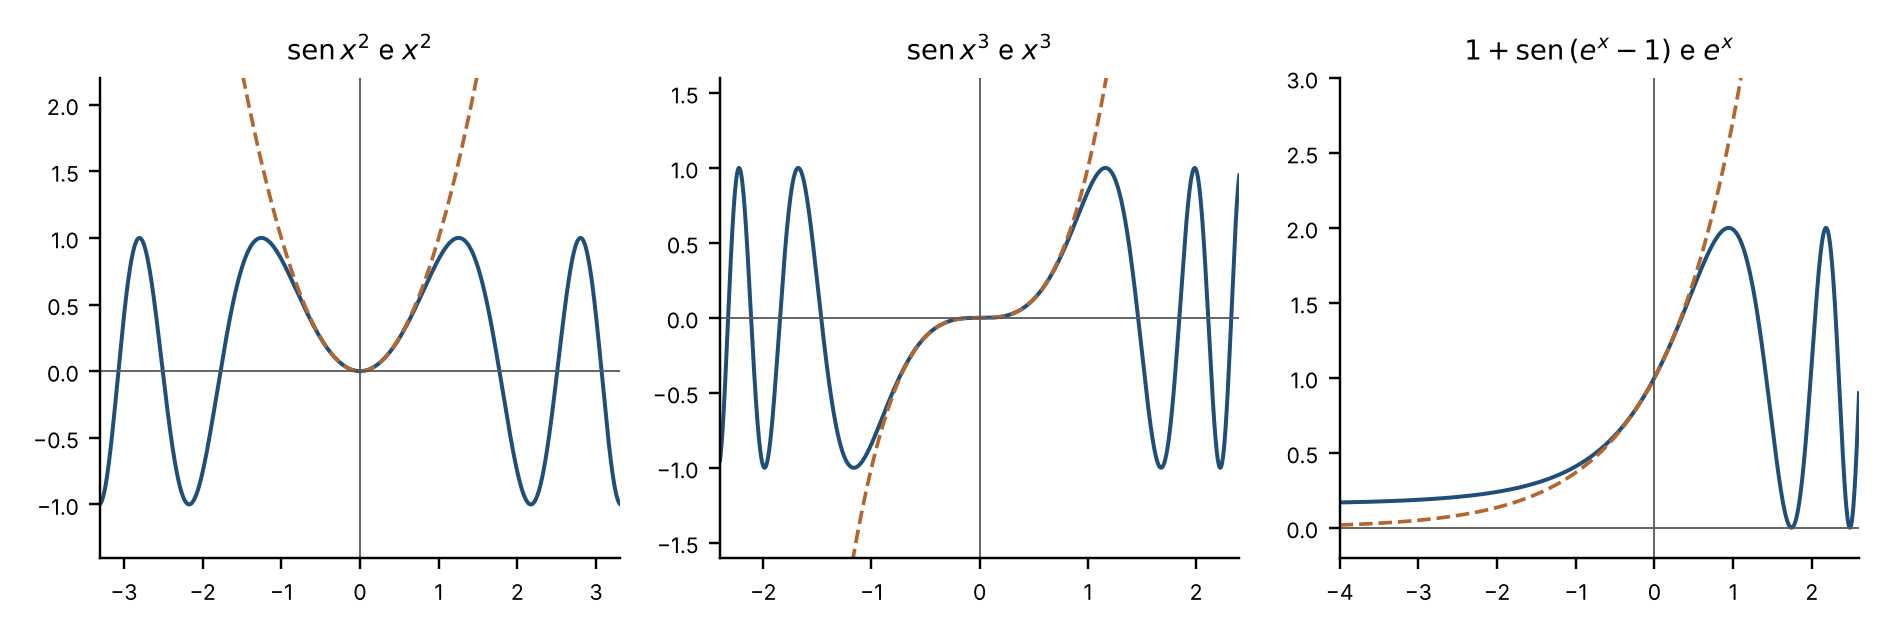
\includegraphics[width=\textwidth]{figure/taylor_composte.png}
\caption{Le funzioni $\sen x^{2}$, $\sen x^{3}$ e $1+\sen(e^{x}-1)$ (in blu) e le loro approssimazioni
vicino all'origine $x^{2}$, $x^{3}$, $e^{x}$ (tratteggio rame). Lontano dall'origine la
somiglianza scompare: $\sen x^{2}$ e $\sen x^{3}$ oscillano sempre più rapidamente, e
$1+\sen(e^{x}-1)$ oscilla per $x\to+\infty$ mentre tende a $1+\sen(-1)>0$ per $x\to-\infty$
(\texttt{python/fig\_taylor\_composte.py}).}
\label{fig:taylor-composte}
\end{figure}

Il secondo procedimento consiste nell'integrare uno sviluppo noto.

\begin{lemma}[Integrazione degli o piccoli]\label{lem:integrazione-o}
Sia $m\ge0$ un intero, e sia $g$ continua in un intorno $I$ di $0$, con $g(t)=o(t^{m})$ per
$t\to0$. Allora
\begin{equation}\label{eq:integrazione-o}
  \int_{0}^{x}g(t)\,dt=o(x^{m+1}) \qquad (x\to0) .
\end{equation}
\end{lemma}

\begin{schema}
\Ipotesi{$m\ge0$ intero; \ $g$ continua in $I\ni0$; \ $\frac{g(t)}{t^{m}}\to0$ per $t\to0$.}
\Tesi{$\frac1{x^{m+1}}\int_{0}^{x}g(t)\,dt\to0$ per $x\to0$.}
\end{schema}

\begin{strategia}
Vicino a $0$ si ha $\abs{g(t)}\le\epsilon\abs t^{m}$; integrando la disuguaglianza tra $0$ e $x$ si
ottiene una stima con $\frac{\epsilon\abs x^{m+1}}{m+1}$.
\end{strategia}

\begin{dimostrazione}
Sia $\epsilon>0$. Per l'ipotesi esiste $\delta>0$, che possiamo scegliere in modo che
$(-\delta,\delta)\subseteq I$, tale che $\abs{g(t)}\le\epsilon\abs t^{m}$ per $\abs t<\delta$
(anche per $t=0$, perché $g(0)=\lim_{t\to0}g(t)=0$ per la continuità). Per $0<\abs x<\delta$, per il
\cref{teo:valore-assoluto} e il confronto, applicati nell'intervallo di estremi $0$ e $x$,
\[
  \Bigl|\int_{0}^{x}g(t)\,dt\Bigr|\le\Bigl|\int_{0}^{x}\epsilon\abs t^{m}\,dt\Bigr|=\frac{\epsilon\abs x^{m+1}}{m+1}\le\epsilon\abs x^{m+1} ,
\]
cioè $\Bigl|\frac1{x^{m+1}}\int_{0}^{x}g\Bigr|\le\epsilon$, che è la tesi.
\end{dimostrazione}

Ne segue che uno sviluppo della derivata si può integrare «termine a termine»: se $f'$ è
continua vicino a $0$ e $f'(x)=\sum_{k=0}^{n}a_{k}x^{k}+o(x^{n})$, allora, per la formula
fondamentale e il lemma,
\begin{equation}\label{eq:integrazione-termine}
  f(x)=f(0)+\int_{0}^{x}f'(t)\,dt=f(0)+\sum_{k=0}^{n}\frac{a_{k}}{k+1}\,x^{k+1}+o(x^{n+1}) .
\end{equation}
Il procedimento inverso, cioè derivare uno sviluppo termine a termine, non è lecito in
generale: $x^{3}\sen\frac1x=o(x^{2})$, ma la sua derivata $3x^{2}\sen\frac1x-x\cos\frac1x$ non è $o(x)$.

\subsection{Lo sviluppo dell'arcotangente}

Applichiamo l'idea dell'integrazione all'arcotangente, le cui derivate successive sono
sempre più complicate. Il punto di partenza è che la sua derivata $\frac1{1+t^{2}}$ è la somma
di una progressione geometrica di ragione $-t^{2}$, a meno di un resto esplicito; in questo
modo otteniamo non soltanto lo sviluppo, ma anche una stima del resto valida per
\emph{ogni} $x$.

\begin{proposizione}[Sviluppo dell'arcotangente]\label{prop:sviluppo-arctg}
Per ogni $n\in\N\cup\set0$ e ogni $x\in\R$,
\begin{equation}\label{eq:sviluppo-arctg}
\begin{gathered}
  \operatorname{arctg}x=x-\frac{x^{3}}3+\frac{x^{5}}5-\dots+(-1)^{n}\frac{x^{2n+1}}{2n+1}+R(x),\\
  R(x)=(-1)^{n+1}\int_{0}^{x}\frac{t^{2n+2}}{1+t^{2}}\,dt, \qquad
  \abs{R(x)}\le\frac{\abs x^{2n+3}}{2n+3} .
\end{gathered}
\end{equation}
In particolare $R(x)=o(x^{2n+2})$ per $x\to0$, e il polinomio a secondo membro è il polinomio
di Taylor di ordine $2n+2$ dell'arcotangente in $0$.
\end{proposizione}

\begin{schema}
\Ipotesi{$n\ge0$ intero; \ $x\in\R$.}
\Tesi{la \eqref{eq:sviluppo-arctg}, con il resto in forma integrale e
$\abs{R(x)}\le\frac{\abs x^{2n+3}}{2n+3}$; \ $R(x)=o(x^{2n+2})$.}
\end{schema}

\begin{strategia}
La somma della progressione geometrica $1-t^{2}+t^{4}-\dots+(-1)^{n}t^{2n}$ è
$\frac{1-(-t^{2})^{n+1}}{1+t^{2}}$: dunque $\frac1{1+t^{2}}$ è uguale a questa somma più il resto esplicito
$\frac{(-1)^{n+1}t^{2n+2}}{1+t^{2}}$. Integrando tra $0$ e $x$, la somma dà il polinomio e il resto si
stima con $t^{2n+2}$, perché $1+t^{2}\ge1$. L'unicità del polinomio di Taylor fa il resto.
\end{strategia}

\begin{dimostrazione}
Per la formula della somma della progressione geometrica (\cref{prop:geometrica}) con
ragione $-t^{2}\neq1$,
\[
  \sum_{k=0}^{n}(-t^{2})^{k}=\frac{1-(-t^{2})^{n+1}}{1+t^{2}} ,
\]
cioè
\[
  \frac1{1+t^{2}}=\sum_{k=0}^{n}(-1)^{k}t^{2k}+(-1)^{n+1}\frac{t^{2n+2}}{1+t^{2}} .
\]
Integriamo tra $0$ e $x$: per la formula fondamentale, poiché $D\operatorname{arctg}t=\frac1{1+t^{2}}$
\eqref{eq:derivata-arctg} e $\operatorname{arctg}0=0$,
\[
  \operatorname{arctg}x=\sum_{k=0}^{n}(-1)^{k}\frac{x^{2k+1}}{2k+1}+R(x), \qquad
  R(x)=(-1)^{n+1}\int_{0}^{x}\frac{t^{2n+2}}{1+t^{2}}\,dt .
\]
Poiché $0\le\frac{t^{2n+2}}{1+t^{2}}\le t^{2n+2}$, per il confronto
$\abs{R(x)}\le\bigl|\int_{0}^{x}t^{2n+2}\,dt\bigr|=\frac{\abs x^{2n+3}}{2n+3}$. Ne segue
$\bigl|\frac{R(x)}{x^{2n+2}}\bigr|\le\frac{\abs x}{2n+3}\to0$, cioè $R(x)=o(x^{2n+2})$; per la
\cref{prop:unicita-taylor} il polinomio trovato è il polinomio di Taylor di ordine $2n+2$.
\end{dimostrazione}

Lo stesso ragionamento, con $\frac1{1+t}=\sum_{k=0}^{n-1}(-t)^{k}+\frac{(-t)^{n}}{1+t}$ ($n\ge1$), ritrova lo
sviluppo \eqref{eq:taylor-log} del logaritmo, con il resto
$R(x)=(-1)^{n}\int_{0}^{x}\frac{t^{n}}{1+t}\,dt$ e la stima $\abs{R(x)}\le\frac{x^{n+1}}{n+1}$ per ogni $x\ge0$ (per
$-1<x<0$ si trova invece $\abs{R(x)}\le\frac{\abs x^{n+1}}{(n+1)(1+x)}$).

La stima della \cref{prop:sviluppo-arctg} dice di più del resto di Peano. Se $\abs x\le1$,
il resto tende a zero per $n\to+\infty$: il valore di $\operatorname{arctg}x$ è il limite dei
polinomi. Per $x=1$ si ottiene la \emph{serie di Leibniz}
\begin{equation}\label{eq:serie-leibniz}
  \frac\pi4=\operatorname{arctg}1=1-\frac13+\frac15-\frac17+\cdots ,
\end{equation}
nel senso che le somme parziali differiscono da $\frac\pi4$ al più di $\frac1{2n+3}$. La
convergenza è però lentissima: per garantire un errore su $\pi$ inferiore a $10^{-6}$ la
stima richiede circa due milioni di termini. Molto più efficiente è la
\emph{formula di Machin}
\begin{equation}\label{eq:machin}
  \frac\pi4=4\operatorname{arctg}\frac15-\operatorname{arctg}\frac1{239}
\end{equation}
(che si verifica con la formula di addizione della tangente, \cref{es:machin}): con
$x=\frac15$ il resto è al più $\frac{5^{-(2n+3)}}{2n+3}$, e ogni termine aggiunge circa una cifra e
mezza. Se invece $\abs x>1$ la stima non serve, e infatti i polinomi di Taylor
dell'arcotangente si allontanano dalla funzione al crescere del grado
(\cref{fig:taylor-arctg}): a differenza di quanto accade per il seno
(\cref{fig:taylor-seno}), un'ottima approssimazione vicino a $0$ non garantisce nulla
lontano da $0$, anche per una funzione derivabile infinite volte su tutto $\R$. La ragione profonda di questo
comportamento è nascosta nel campo complesso: la funzione $\frac1{1+t^{2}}$, derivata
dell'arcotangente, non è definita nei numeri complessi $t=\pm i$, che distano $1$
dall'origine. La chiarisce la teoria delle serie di potenze, che si studia nei corsi
successivi e a cui accenneremo alla fine del \cref{cap:serie}.

\begin{figure}[htb]
\centering
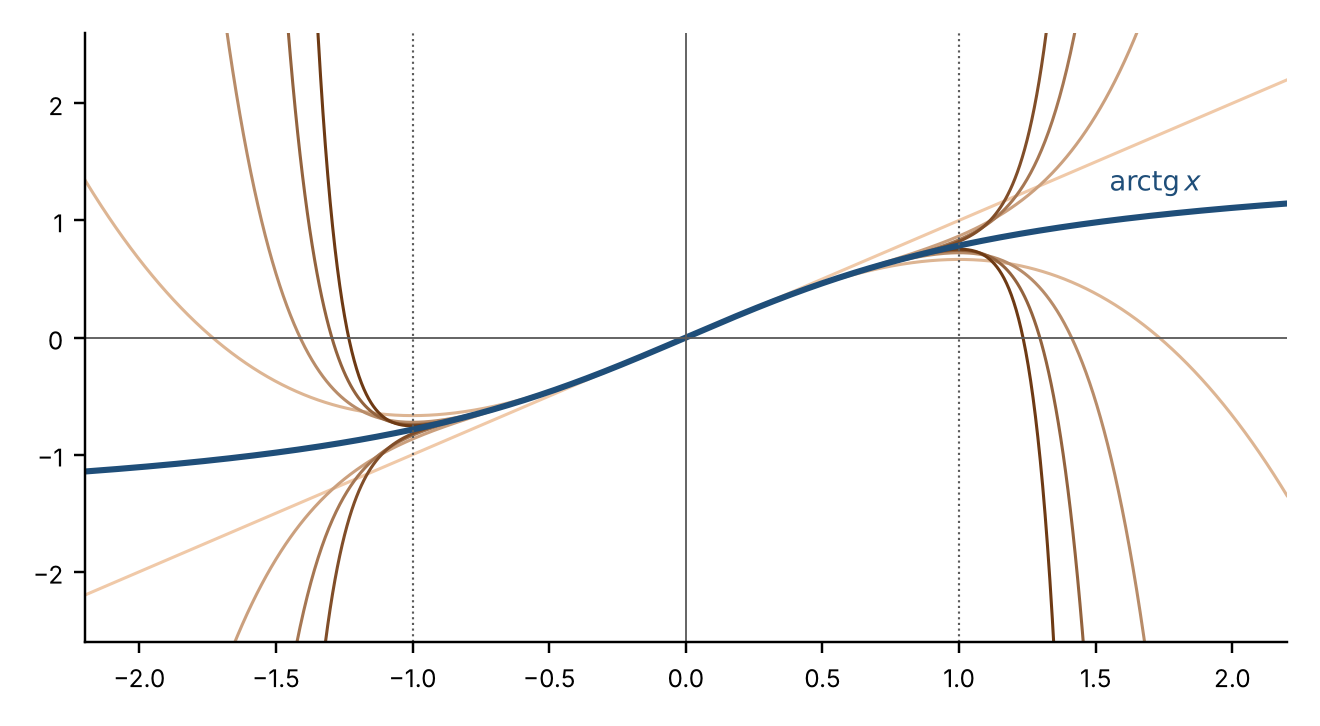
\includegraphics[width=\textwidth]{figure/taylor_arctg.png}
\caption{L'arcotangente (blu) e i suoi polinomi di Taylor in $0$ di grado $1,3,5,\dots,15$
(rame, più scuri al crescere del grado). In $[-1,1]$ i polinomi si avvicinano alla
funzione; per $\abs x>1$ se ne allontanano sempre di più
(\texttt{python/fig\_taylor\_arctg.py}).}
\label{fig:taylor-arctg}
\end{figure}

\begin{python}[Le cifre di $\pi$: serie di Leibniz e formula di Machin]
from fractions import Fraction as F
import math

def arctg(x, n):
    """T(x) = x - x^3/3 + ... + (-1)^n x^(2n+1)/(2n+1)."""
    return sum((-1)**k * x**(2*k + 1) / (2*k + 1)
               for k in range(n + 1))

for n in (10, 100, 1000):
    print(f"Leibniz, n = {n:4d}:  4*T = {4 * arctg(1.0, n):.10f}")
for n in (2, 4, 6, 8):
    p = 4 * (4 * arctg(F(1, 5), n) - arctg(F(1, 239), n))
    print(f"Machin,  n = {n}:     4*T = {float(p):.15f}")
print(f"                  pi    = {math.pi:.15f}")
\end{python}
\begin{risultato}
Leibniz, n =   10:  4*T = 3.2323158094
Leibniz, n =  100:  4*T = 3.1514934011
Leibniz, n = 1000:  4*T = 3.1425916543
Machin,  n = 2:     4*T = 3.141621029325035
Machin,  n = 4:     4*T = 3.141592682404399
Machin,  n = 6:     4*T = 3.141592653623555
Machin,  n = 8:     4*T = 3.141592653589836
                  pi    = 3.141592653589793
\end{risultato}

\begin{idea}[La distanza dell'orizzonte]
Da un velivolo che vola alla quota $h$ sopra una Terra sferica di raggio
$R\approx6371$~km, la visuale verso l'orizzonte è tangente alla superficie
(\cref{fig:orizzonte}). Se $\vartheta$ è l'angolo al centro della Terra tra la verticale del
velivolo e il punto di tangenza, il triangolo rettangolo formato dal centro, dal velivolo
e dal punto di tangenza dà $\cos\vartheta=\frac R{R+h}$, cioè $1-\cos\vartheta=\frac h{R+h}$, e la
distanza dell'orizzonte misurata sulla superficie è $d=R\vartheta$. Per la
\eqref{eq:taylor-cos}, $1-\cos\vartheta=\frac{\vartheta^{2}}2\,(1+o(1))$ per $\vartheta\to0$; poiché $h$ è piccolo
rispetto a $R$, anche $\vartheta$ è piccolo, e
\begin{equation}\label{eq:orizzonte}
  \vartheta\approx\sqrt{\frac{2h}{R}}, \qquad d\approx\sqrt{2Rh} .
\end{equation}
A $10\,000$~m di quota l'orizzonte dista circa $\sqrt{2\cdot6371\cdot10}\approx357$~km. La stessa
formula dà la portata «ottica» di un radar o di un collegamento radio in visibilità; in
radiotecnica, per tener conto della rifrazione atmosferica, si usa un raggio terrestre
equivalente pari ai $\frac43$ di quello reale. Il programma confronta la formula
approssimata con quella esatta $d=R\arccos\frac R{R+h}$. Si vedrà che l'approssimazione
sovrastima leggermente la distanza; l'\cref{es:orizzonte-secondo-ordine} ne spiega il
motivo e ne calcola l'errore.
\end{idea}

\begin{figure}[htb]
\centering
\begin{tikzpicture}[scale=1.0]
  \fill[blu!8] (0,0) circle (2.2);
  \draw[blu, thick] (0,0) circle (2.2);
  \coordinate (O) at (0,0);
  \coordinate (A) at (0,3.3);
  \coordinate (T) at ({2.2*sin(48.19)},{2.2*cos(48.19)});
  \draw[grigio] (O) -- (A);
  \draw[grigio] (O) -- (T);
  \draw[rame, thick] (A) -- (T) -- ($(T)!-0.35!(A)$);
  \fill[rame] (A) circle (1.8pt) node[above, font=\scriptsize] {velivolo};
  \fill (T) circle (1.4pt) node[above right, font=\scriptsize] {orizzonte};
  \draw[grigio] (0,0.5) arc (90:41.81:0.5);
  \node[font=\scriptsize] at (0.33,0.78) {$\vartheta$};
  \draw[verde!70!black, very thick] (0,2.2) arc (90:41.81:2.2);
  \node[font=\scriptsize, verde!70!black] at (0.8,1.78) {$d$};
  \node[font=\scriptsize, left] at (0,1.1) {$R$};
  \node[font=\scriptsize, left] at (0,2.75) {$h$};
  \coordinate (P) at ($(T)!0.2cm!(O)$);
  \coordinate (Q) at ($(T)!0.2cm!(A)$);
  \draw[grigio] (P) -- ($(P)+(Q)-(T)$) -- (Q);
\end{tikzpicture}
\caption{La distanza dell'orizzonte. La visuale dal velivolo al punto di tangenza è
perpendicolare al raggio; l'angolo al centro $\vartheta$ verifica $\cos\vartheta=\frac R{R+h}$, e
la distanza sulla superficie è l'arco $d=R\vartheta$. La quota è fortemente esagerata.}
\label{fig:orizzonte}
\end{figure}

\begin{python}[Distanza dell'orizzonte: formula esatta e approssimata]
import math

R = 6371.0                                 # raggio terrestre [km]
print(" h [km]   esatta [km]   sqrt(2Rh) [km]   differenza")
for h in (0.1, 1.0, 3.0, 10.0, 12.0):
    d = R * math.acos(R / (R + h))         # arco R*theta
    a = math.sqrt(2 * R * h)
    print(f"{h:6.1f}   {d:10.2f}    {a:12.2f}     {a - d:8.3f}")
\end{python}
\begin{risultato}
 h [km]   esatta [km]   sqrt(2Rh) [km]   differenza
   0.1        35.70           35.70        0.000
   1.0       112.87          112.88        0.007
   3.0       195.48          195.51        0.038
  10.0       356.73          356.96        0.233
  12.0       390.72          391.03        0.307
\end{risultato}

\begin{notastorica}[Madhava, Gregory, Leibniz, Machin]
Lo sviluppo dell'arcotangente fu scoperto in India, intorno al 1400, da Madhava di
Sangamagrama, fondatore della scuola astronomica e matematica del Kerala, che ne ricavò
anche la serie \eqref{eq:serie-leibniz}; i suoi risultati, tramandati in testi in sanscrito
e in malayalam, rimasero sconosciuti in Europa. Qui la serie fu riscoperta da James Gregory
(1671) e da Leibniz (1673--1674), che vi giunse con il suo teorema di trasmutazione. Nel
1706 l'astronomo inglese John Machin, con la formula \eqref{eq:machin}, calcolò cento
cifre decimali di $\pi$ a mano; formule dello stesso tipo sono state usate nei record di
calcolo di $\pi$ fino al 2002, quando Yasumasa Kanada ne calcolò con il computer più di
mille miliardi di cifre.
\end{notastorica}

%% ----------------------------------------------------------------------------
%%  §10.2  L'algebra degli o piccoli e il calcolo dei limiti
%% ----------------------------------------------------------------------------
\section{L'algebra degli o piccoli e il calcolo dei limiti}
\label{sec:o-piccoli}

La formula di Taylor con il resto di Peano è lo strumento più efficace per il calcolo
dei limiti che si presentano in forma indeterminata. Cominciamo con un esempio, che ci
mostrerà di quali regole di calcolo abbiamo bisogno.

\begin{esempio}\label{es:limite-taylor-1}
Calcoliamo
\begin{equation}\label{eq:limite-taylor-1}
  \lim_{x\to0}\Bigl(\frac1{x^{2}}-\frac1{x\sen x}\Bigr) ,
\end{equation}
che si presenta nella forma indeterminata $+\infty-(+\infty)$. Riducendo allo stesso
denominatore e usando lo sviluppo $\sen x=x-\frac{x^{3}}6+o(x^{4})$ (la \eqref{eq:taylor-sen} con
$n=1$),
\[
  \frac1{x^{2}}-\frac1{x\sen x}=\frac{\sen x-x}{x^{2}\sen x}
  =\frac{-\frac{x^{3}}6+o(x^{4})}{x^{3}-\frac{x^{5}}6+o(x^{6})} ,
\]
dove abbiamo usato il fatto che $x^{2}\cdot o(x^{4})=o(x^{6})$. Dividendo numeratore e
denominatore per $x^{3}$, e osservando che $\frac{o(x^{4})}{x^{3}}=x\cdot\frac{o(x^{4})}{x^{4}}\to0$ e che
$\frac{o(x^{6})}{x^{3}}\to0$, si ottiene
\[
  \lim_{x\to0}\frac{-\frac16+\frac{o(x^{4})}{x^{3}}}{1-\frac{x^{2}}6+\frac{o(x^{6})}{x^{3}}}=-\frac16 .
\]
Si noti la scelta dell'ordine dello sviluppo. Con il solo $\sen x=x+o(x^{2})$ il numeratore
sarebbe stato $o(x^{2})$, e il rapporto $\frac{o(x^{2})}{x^{3}}$ è ancora indeterminato: occorre
spingere lo sviluppo fino al primo termine che \emph{non si elide}.
\end{esempio}

Nel calcolo precedente abbiamo trattato il simbolo $o(\cdot)$ come se fosse un numero,
sommandolo, moltiplicandolo per potenze, dividendolo. Occorre dare un senso preciso a
queste operazioni.

\begin{notazione}[Uguaglianze con gli o piccoli]
In una formula, il simbolo $o(x^{n})$ (per $x\to0$) indica \emph{una qualsiasi} funzione $f$
tale che $\frac{f(x)}{x^{n}}\to0$; per $n=0$, $o(1)$ indica una qualsiasi funzione infinitesima.
Un'uguaglianza tra espressioni che contengono simboli $o$, come $x^{2}\cdot o(x^{4})=o(x^{6})$,
significa: \emph{ogni} funzione della forma scritta a sinistra è anche della forma
scritta a destra. Queste uguaglianze vanno quindi lette da sinistra a destra, e non sono
simmetriche: $o(x^{2})=o(x)$ è vera (ogni funzione che è $o(x^{2})$ è anche $o(x)$), mentre
$o(x)=o(x^{2})$ è falsa (si pensi a $x^{3/2}$, per $x>0$).
\end{notazione}

\begin{proposizione}[Algebra degli o piccoli]\label{prop:algebra-o}
Per $x\to0$ e per ogni coppia di interi $m,n\ge0$ valgono le proprietà
\begin{align}
  & o(x^{n})+o(x^{n})=o(x^{n}), \qquad o(x^{n})-o(x^{n})=o(x^{n}); \label{eq:o-somma}\\
  & c\cdot o(x^{n})=o(x^{n}), \qquad o(c\,x^{n})=o(x^{n}) \qquad (c\neq0 \text{ costante}); \label{eq:o-costante}\\
  & x^{m}\cdot o(x^{n})=o(x^{m+n}); \label{eq:o-potenza}\\
  & o(x^{m})\cdot o(x^{n})=o(x^{m+n}); \label{eq:o-prodotto}\\
  & o(x^{m})=o(x^{n}) \ \text{ se } m\ge n, \qquad x^{m}=o(x^{n}) \ \text{ se } m>n; \label{eq:o-ordine}\\
  & \frac{o(x^{n})}{x^{m}}=o(x^{n-m}) \qquad (m\le n); \label{eq:o-quoziente}\\
  & o\bigl(o(x^{n})\bigr)=o(x^{n}); \label{eq:o-o}\\
  & o\bigl(x^{n}+o(x^{n})\bigr)=o(x^{n}). \label{eq:o-somma-interna}
\end{align}
\end{proposizione}

\begin{schema}
\Ipotesi{$x\to0$; \ $m,n\ge0$ interi; \ ogni simbolo $o(g)$ denota una funzione $f$ con
$\frac fg\to0$.}
\Tesi{ogni funzione della forma a primo membro delle
\eqref{eq:o-somma}--\eqref{eq:o-somma-interna} è anche della forma a secondo membro.}
\end{schema}

\begin{strategia}
Ogni proprietà si traduce in un'affermazione sui limiti: si scrivono esplicitamente le
funzioni che compaiono a primo membro, si divide per la potenza che compare a secondo
membro e si riconosce, con un'opportuna moltiplicazione e divisione, un prodotto o una
somma di quozienti che tendono a zero per ipotesi. Le ultime due proprietà, in cui un o
piccolo compare \emph{dentro} un altro, richiedono di passare attraverso la funzione
intermedia.
\end{strategia}

\begin{dimostrazione}
Siano $f$ e $g$ funzioni definite vicino a $0$ (escluso al più $0$).

\eqref{eq:o-somma}: se $\frac{f(x)}{x^{n}}\to0$ e $\frac{g(x)}{x^{n}}\to0$, allora
$\frac{f(x)\pm g(x)}{x^{n}}=\frac{f(x)}{x^{n}}\pm\frac{g(x)}{x^{n}}\to0$.

\eqref{eq:o-costante}: se $\frac{f(x)}{x^{n}}\to0$ allora $\frac{c\,f(x)}{x^{n}}=c\,\frac{f(x)}{x^{n}}\to0$; se invece
$\frac{f(x)}{c\,x^{n}}\to0$, allora $\frac{f(x)}{x^{n}}=c\,\frac{f(x)}{c\,x^{n}}\to0$.

\eqref{eq:o-potenza}: se $\frac{f(x)}{x^{n}}\to0$, allora $\frac{x^{m}f(x)}{x^{m+n}}=\frac{f(x)}{x^{n}}\to0$.

\eqref{eq:o-prodotto}: se $\frac{f(x)}{x^{m}}\to0$ e $\frac{g(x)}{x^{n}}\to0$, allora
$\frac{f(x)g(x)}{x^{m+n}}=\frac{f(x)}{x^{m}}\cdot\frac{g(x)}{x^{n}}\to0$.

\eqref{eq:o-ordine}: se $m\ge n$ e $\frac{f(x)}{x^{m}}\to0$, allora $\frac{f(x)}{x^{n}}=x^{m-n}\,\frac{f(x)}{x^{m}}\to0$,
perché $x^{m-n}$ vale $1$ se $m=n$ e tende a $0$ se $m>n$. Se $m>n$, inoltre,
$\frac{x^{m}}{x^{n}}=x^{m-n}\to0$.

\eqref{eq:o-quoziente}: se $\frac{f(x)}{x^{n}}\to0$, allora $\frac{f(x)/x^{m}}{x^{n-m}}=\frac{f(x)}{x^{n}}\to0$.

\eqref{eq:o-o}: sia $g=o(x^{n})$, con $g(x)\neq0$ per $x\neq0$ (condizione richiesta dalla
\cref{def:o-piccolo} perché abbia senso scrivere $o(g)$), e sia $f=o(g)$. Allora
\[
  \frac{f(x)}{x^{n}}=\frac{f(x)}{g(x)}\cdot\frac{g(x)}{x^{n}}\longrightarrow0\cdot0=0 .
\]

\eqref{eq:o-somma-interna}: sia $g(x)=x^{n}+h(x)$ con $h=o(x^{n})$, e sia $f=o(g)$. Poiché
$\frac{g(x)}{x^{n}}=1+\frac{h(x)}{x^{n}}\to1$, la funzione $g$ è diversa da zero vicino a $0$ (per la
permanenza del segno), e
\[
  \frac{f(x)}{x^{n}}=\frac{f(x)}{g(x)}\cdot\frac{g(x)}{x^{n}}
  =\frac{f(x)}{g(x)}\cdot\Bigl(1+\frac{h(x)}{x^{n}}\Bigr)\longrightarrow0\cdot1=0 . \qedhere
\]
\end{dimostrazione}

\begin{attenzione}
Non è lecito scrivere $o(x^{n})-o(x^{n})=0$: i due simboli denotano, in generale, due funzioni
\emph{diverse}, entrambe trascurabili rispetto a $x^{n}$, e la loro differenza è soltanto
un'altra funzione trascurabile rispetto a $x^{n}$, come afferma la \eqref{eq:o-somma}. Ad
esempio $x^{3}=o(x^{2})$ e $2x^{3}=o(x^{2})$, ma $x^{3}-2x^{3}=-x^{3}\neq0$. Per la stessa ragione un
rapporto come $\frac{o(x^{n})}{o(x^{n})}$ non ha alcun significato preciso: può tendere a qualunque
valore, o non avere limite.
\end{attenzione}

Le proprietà \eqref{eq:o-o} e \eqref{eq:o-somma-interna} si generalizzano a un argomento che
sia un qualunque infinitesimo con parte principale nota; è la forma che useremo più
spesso.

\begin{corollario}[o piccoli di infinitesimi con parte principale]\label{cor:o-composto}
Sia $\varphi(x)=a\,x^{k}+o(x^{k})$ per $x\to0$, con $a\neq0$ e $k\ge1$. Allora, per ogni intero
$m\ge1$,
\begin{equation}\label{eq:o-composto}
  \varphi(x)^{m}=a^{m}x^{km}+o(x^{km}), \qquad o\bigl(\varphi(x)^{m}\bigr)=o(x^{km}) .
\end{equation}
\end{corollario}

\begin{schema}
\Ipotesi{$\frac{\varphi(x)}{x^{k}}\to a\neq0$ per $x\to0$; \ $m\ge1$ intero.}
\Tesi{$\frac{\varphi(x)^{m}}{x^{km}}\to a^{m}$; \ se $\frac{f(x)}{\varphi(x)^{m}}\to0$, allora $\frac{f(x)}{x^{km}}\to0$.}
\end{schema}

\begin{strategia}
Tutto discende dal fatto che il rapporto $\frac{\varphi(x)}{x^{k}}$ tende ad $a\neq0$: la potenza
$m$-esima di questo rapporto tende ad $a^{m}$, il che dà la prima uguaglianza. Per la
seconda si procede come per la \eqref{eq:o-o}, scrivendo $\frac{f}{x^{km}}$ come prodotto di
$\frac{f}{\varphi^{m}}$, che tende a zero, e di $\bigl(\frac{\varphi}{x^{k}}\bigr)^{m}$, che resta limitato;
la permanenza del segno garantisce che $\varphi$ non si annulli vicino a $0$.
\end{strategia}

\begin{dimostrazione}
Per ipotesi $\frac{\varphi(x)}{x^{k}}=a+\frac{o(x^{k})}{x^{k}}\to a$, e quindi
$\frac{\varphi(x)^{m}}{x^{km}}=\bigl(\frac{\varphi(x)}{x^{k}}\bigr)^{m}\to a^{m}$, cioè
$\varphi(x)^{m}-a^{m}x^{km}=o(x^{km})$. In particolare $\varphi(x)\neq0$ vicino a $0$, per la permanenza
del segno. Se poi $f=o(\varphi^{m})$,
\[
  \frac{f(x)}{x^{km}}=\frac{f(x)}{\varphi(x)^{m}}\cdot\Bigl(\frac{\varphi(x)}{x^{k}}\Bigr)^{m}\longrightarrow0\cdot a^{m}=0 .
  \qedhere
\]
\end{dimostrazione}

Con questo corollario sono giustificati i calcoli fatti nel \cref{sec:taylor-peano} per la
funzione $1+\sen(e^{x}-1)$: con $u=e^{x}-1=x+o(x)$, si ha $u^{3}=x^{3}+o(x^{3})$ e
$o(u^{3})=o(x^{3})$.

Gli sviluppi di Taylor permettono di confrontare tra loro gli infinitesimi in modo
preciso. Fissiamo il linguaggio.

\begin{definizione}[Ordine di infinitesimo, parte principale, equivalenza]
\label{def:parte-principale}\index{infinitesimo!ordine di}\index{parte principale}
Sia $f$ definita vicino a $0$ (escluso al più $0$). Se esistono un numero $a\neq0$ e un
intero $p\ge0$ tali che
\[
  f(x)=a\,x^{p}+o(x^{p}) \qquad (x\to0),
\]
cioè $\frac{f(x)}{x^{p}}\to a\neq0$, si dice che $f$ è un \emph{infinitesimo di ordine $p$} (se $p\ge1$)
e che $a\,x^{p}$ è la sua \emph{parte principale}. Due funzioni $f$ e $g$ si dicono
\emph{equivalenti} per $x\to0$, e si scrive $f\sim g$, se $\frac{f(x)}{g(x)}\to1$.
\end{definizione}

Ad esempio $\sen x-x$ è un infinitesimo di ordine $3$ con parte principale $-\frac{x^{3}}6$, e
$1-\cos x\sim\frac{x^{2}}2$. Il numero $a$ e l'esponente $p$, quando esistono, sono univocamente
determinati: se fosse anche $f(x)=b\,x^{q}+o(x^{q})$ con $q\neq p$, ad esempio $q>p$ (l'altro
caso è simmetrico), dividendo per $x^{p}$ si avrebbe $\frac{f(x)}{x^{p}}\to0\neq a$; e se $q=p$,
allora $a=b=\lim\frac{f(x)}{x^{p}}$. Una funzione con una parte
principale è equivalente a essa. La proposizione che segue riassume il metodo con cui la
formula di Taylor si usa nel calcolo dei limiti di rapporti.

\begin{proposizione}[Principio della parte principale]\label{prop:parte-principale}
Siano $f(x)=a\,x^{p}+o(x^{p})$ e $g(x)=b\,x^{q}+o(x^{q})$ per $x\to0$, con $a,b\neq0$ e
$p,q\ge0$ interi. Allora
\begin{equation}\label{eq:parte-principale}
  \frac{f(x)}{g(x)}=\frac ab\,x^{p-q}\bigl(1+o(1)\bigr) ;
\end{equation}
in particolare $\frac{f(x)}{g(x)}\to\frac ab$ se $p=q$, e $\frac{f(x)}{g(x)}\to0$ se $p>q$, mentre se $p<q$ il
rapporto diverge in valore assoluto.
\end{proposizione}

\begin{schema}
\Ipotesi{$\frac{f(x)}{x^{p}}\to a\neq0$, \ $\frac{g(x)}{x^{q}}\to b\neq0$ per $x\to0$.}
\Tesi{$\frac{f(x)}{g(x)}\sim\frac ab\,x^{p-q}$: nel limite di un rapporto si possono sostituire numeratore
e denominatore con le loro parti principali.}
\end{schema}

\begin{strategia}
Si confronta il rapporto $\frac fg$ con il rapporto delle parti principali, cioè si mostra
che il loro quoziente tende a $1$. Dividendo numeratore per $x^{p}$ e denominatore per
$x^{q}$, questo quoziente diventa il prodotto di $\frac{f(x)/x^{p}}{a}$ e di
$\frac{b}{g(x)/x^{q}}$, che tendono entrambi a $1$ per ipotesi. Il comportamento di $x^{p-q}$
decide poi il limite.
\end{strategia}

\begin{dimostrazione}
Per $x\neq0$ vicino a $0$ (dove $g(x)\neq0$, per la permanenza del segno applicata a
$\frac{g(x)}{x^{q}}\to b\neq0$),
\[
  \frac{f(x)}{g(x)}\cdot\frac b{a\,x^{p-q}}=\frac{f(x)/x^{p}}{a}\cdot\frac{b}{g(x)/x^{q}}\longrightarrow\frac aa\cdot\frac bb=1 .
\]
Le affermazioni sul limite seguono perché $x^{p-q}$ vale $1$ se $p=q$, tende a $0$ se $p>q$
e diverge in valore assoluto se $p<q$.
\end{dimostrazione}

Nell'\cref{es:limite-taylor-1}, ad esempio, il numeratore $\sen x-x$ ha parte principale
$-\frac{x^{3}}6$ e il denominatore $x^{2}\sen x$ ha parte principale $x^{3}$: il limite è $-\frac16$, senza
altri calcoli. Il problema si riduce dunque a trovare la parte principale del numeratore
e del denominatore, cioè il primo termine non nullo dei loro sviluppi.

\begin{esempio}\label{es:limite-taylor-2}
Calcoliamo
\[
  \lim_{x\to0}\Bigl(\frac1x-\frac{\cos x}{x^{3}}+\frac{\sen3x}{3x^{4}}\Bigr)
  =\lim_{x\to0}\frac{3x^{3}-3x\cos x+\sen3x}{3x^{4}} .
\]
Il denominatore ha parte principale $3x^{4}$; occorre dunque sviluppare il numeratore
almeno fino all'ordine $4$. Ponendo $3x$ al posto di $x$ nello sviluppo del seno
(\cref{lem:sostituzione-o} e \eqref{eq:o-costante}) si ottiene $\sen3x=3x-\frac92\,x^{3}+o(x^{4})$;
inoltre, per la \eqref{eq:taylor-cos} e la \eqref{eq:o-potenza},
$3x\cos x=3x\bigl(1-\frac{x^{2}}2+o(x^{3})\bigr)=3x-\frac32\,x^{3}+o(x^{4})$. Allora
\[
  3x^{3}-3x\cos x+\sen3x=3x^{3}-3x+\frac32\,x^{3}+3x-\frac92\,x^{3}+o(x^{4})=o(x^{4}) ,
\]
e il limite vale $\lim_{x\to0}\frac{o(x^{4})}{3x^{4}}=0$. Tutti i termini fino all'ordine $4$ si sono
elisi. Spingendo gli sviluppi di un ordine (o di due) si trova la parte principale del
numeratore, $\frac{19}{10}\,x^{5}$, e quindi, per la \cref{prop:parte-principale}, la funzione
tende a zero come $\frac{19}{30}\,x$ (\cref{es:verifica-19-30}).
\end{esempio}

\begin{esempio}\label{es:limite-taylor-3}
Studiamo il limite della successione
\[
  \lim_{n\to+\infty}\Bigl(\cos\frac1n\Bigr)^{-n^{2}} .
\]
Per la definizione di limite di funzione mediante successioni (\cref{def:limite-funzione}),
con $x_{n}=\frac1n\to0$, basta calcolare il limite di funzione
\[
  \lim_{x\to0}(\cos x)^{-1/x^{2}}=\lim_{x\to0}e^{-\frac{\log\cos x}{x^{2}}} ,
\]
che è della forma indeterminata $1^{\infty}$. Dalla \eqref{eq:taylor-cos}, $\cos x=1+u$ con
$u=-\frac{x^{2}}2+o(x^{3})$; dalla \eqref{eq:taylor-log} con $n=1$, $\log(1+u)=u+o(u)$, e per il
\cref{cor:o-composto} (con $a=-\frac12$, $k=2$, $m=1$) $o(u)=o(x^{2})$. Dunque
\[
  \log\cos x=-\frac{x^{2}}2+o(x^{3})+o(x^{2})=-\frac{x^{2}}2+o(x^{2}) ,
\]
e quindi $-\frac{\log\cos x}{x^{2}}\to\frac12$. Per la continuità dell'esponenziale (\cref{teo:continuita-esponenziale}) entrambi i
limiti valgono $e^{1/2}=\sqrt e$.
\end{esempio}

\begin{figure}[htb]
\centering
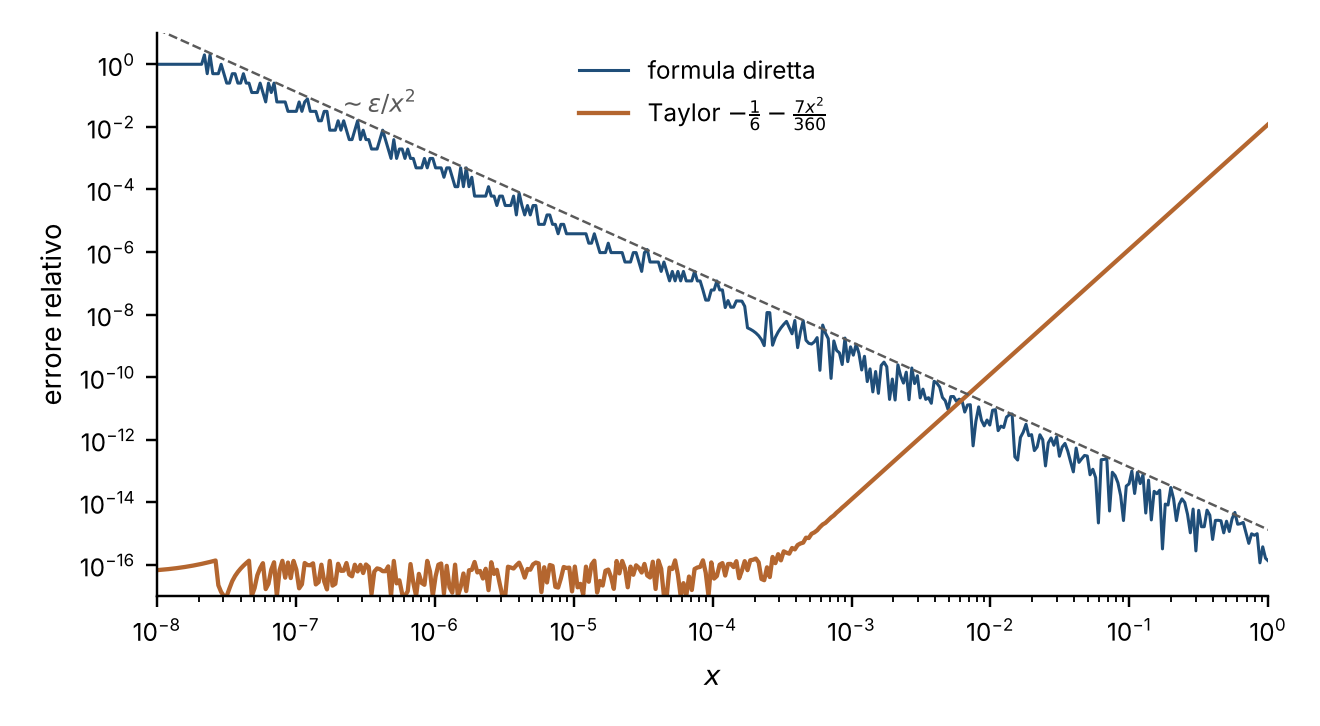
\includegraphics[width=\textwidth]{figure/cancellazione.png}
\caption{Errore relativo nel calcolo di $f(x)=\frac1{x^{2}}-\frac1{x\sen x}$ in aritmetica a
virgola mobile (precisione doppia). La formula diretta (blu) perde cifre come
$\frac{\varepsilon}{x^{2}}$, con $\varepsilon\approx2{,}2\cdot10^{-16}$, per la cancellazione tra due numeri quasi
uguali; il polinomio di Taylor $-\frac16-\frac{7x^{2}}{360}$ (rame) ha un errore che decresce come
$x^{4}$. Le due curve si incrociano per $x$ dell'ordine di $10^{-2}$
(\texttt{python/fig\_cancellazione.py}).}
\label{fig:cancellazione}
\end{figure}

La formula di Taylor non serve soltanto a calcolare limiti «a mano»: è indispensabile
anche nel calcolo numerico. Nel \cref{cap:funzioni-continue} abbiamo incontrato il
fenomeno della \emph{cancellazione}, a proposito di $1-\cos x$ e delle funzioni
\texttt{log1p} ed \texttt{expm1}. La funzione dell'\cref{es:limite-taylor-1}, calcolata con
un computer per $x$ piccolo, ne è un esempio estremo: è la differenza di due numeri
grandi e quasi uguali, ciascuno affetto da un errore di arrotondamento relativo
dell'ordine di $\varepsilon\approx2{,}2\cdot10^{-16}$, e quindi da un errore assoluto dell'ordine di
$\frac\varepsilon{x^{2}}$, che la sottrazione non elimina. Per $x=10^{-8}$ il risultato è privo di
significato. Lo sviluppo $-\frac16-\frac{7x^{2}}{360}+o(x^{3})$ non soffre di questo difetto
(\cref{fig:cancellazione}): la formula di Taylor è il rimedio \emph{sistematico} alla
cancellazione, perché esegue la sottrazione «sulla carta», una volta per tutte. Le
librerie numeriche seguono la stessa idea: per $x$ vicino a zero calcolano funzioni come
\texttt{expm1} e \texttt{log1p} con approssimazioni polinomiali o razionali costruite in
modo da non formare la differenza (i loro coefficienti non sono esattamente quelli di
Taylor, come vedremo nel \cref{sec:tabulazione}), e passano alla formula diretta soltanto
quando la cancellazione non è più pericolosa.

\begin{python}[Limiti con la formula di Taylor: verifica simbolica e numerica]
import math
import sympy as sp
from mpmath import mp, mpf, sin as msin

x = sp.symbols('x')
f = 1 / x**2 - 1 / (x * sp.sin(x))
print(sp.series(f, x, 0, 4))
g = 1 / x - sp.cos(x) / x**3 + sp.sin(3 * x) / (3 * x**4)
print(sp.series(g, x, 0, 3))
print(sp.limit(sp.cos(x)**(-1 / x**2), x, 0))

mp.dps = 40                         # 40 cifre: valore "esatto"
print("     x      formula diretta      Taylor       esatto")
for k in (1, 3, 5, 7, 8):
    t = 10.0**(-k)
    d = 1 / t**2 - 1 / (t * math.sin(t))
    p = -1 / 6 - 7 * t**2 / 360
    e = 1 / mpf(t)**2 - 1 / (mpf(t) * msin(mpf(t)))
    print(f"  1e-{k}  {d:17.12f}  {p:14.12f}  {float(e):14.12f}")
\end{python}
\begin{risultato}
-1/6 - 7*x**2/360 + O(x**4)
19*x/30 + O(x**3)
exp(1/2)
     x      formula diretta      Taylor       esatto
  1e-1    -0.166861316348  -0.166861111111  -0.166861316348
  1e-3    -0.166666686186  -0.166666686111  -0.166666686111
  1e-5    -0.166667938232  -0.166666666669  -0.166666666669
  1e-7    -0.156250000000  -0.166666666667  -0.166666666667
  1e-8     0.000000000000  -0.166666666667  -0.166666666667
\end{risultato}

\begin{notastorica}[I simboli di Landau]
Il simbolo $O$ («o grande»: $f=O(g)$ se $\frac fg$ è limitato) fu introdotto dal teorico dei
numeri tedesco Paul Bachmann nel 1894, nel secondo volume della sua \emph{Zahlentheorie}.
Edmund Landau lo adottò e vi affiancò il simbolo $o$ nel suo trattato sulla distribuzione
dei numeri primi (1909), e da allora entrambi portano il suo nome. L'uso sistematico
degli sviluppi di Taylor per il calcolo dei limiti, però, è molto più antico: già i
matematici del Settecento, a partire da Eulero, trattavano le funzioni come «polinomi
infiniti» e ne confrontavano i termini di grado più basso, anche se senza un controllo
rigoroso del resto. È proprio questo controllo che i simboli di Landau e la formula di
Peano permettono di esercitare con poca fatica.
\end{notastorica}

%% ----------------------------------------------------------------------------
%%  §10.3  La formula di Taylor con il resto integrale
%% ----------------------------------------------------------------------------
\section{La formula di Taylor con il resto integrale}
\label{sec:resto-integrale}

Il resto di Peano descrive il comportamento dell'errore $R_{n}(x)=f(x)-T_{n}(x)$ per
$x\to x_{0}$, ma non dice nulla sul suo valore per un $x$ \emph{fissato}: sapere che
$R_{n}(x)=o\bigl((x-x_{0})^{n}\bigr)$ non permette di affermare, ad esempio, che l'errore
commesso calcolando $\sen\frac1{10}$ con il polinomio $x-\frac{x^{3}}6$ è minore di $10^{-7}$. Per
questo occorre un'espressione esplicita del resto. Se la funzione è abbastanza regolare,
il calcolo integrale la fornisce.

\begin{teorema}[Formula di Taylor con il resto integrale]\label{teo:resto-integrale}
\index{formula di Taylor!con il resto integrale}
Sia $f$ derivabile $n+1$ volte nell'intervallo $[a,b]$, con derivata $f^{(n+1)}$ continua
(cioè $f$ di classe $C^{n+1}$ in $[a,b]$), e sia $x_{0}\in[a,b]$. Allora il resto
$R_{n}(x)=f(x)-T_{n}(x)$ della formula di Taylor di ordine $n$ con centro $x_{0}$ si
rappresenta nella forma
\begin{equation}\label{eq:resto-integrale}
  R_{n}(x)=\int_{x_{0}}^{x}\frac{(x-t)^{n}}{n!}\,f^{(n+1)}(t)\,dt \qquad\perogni x\in[a,b] .
\end{equation}
\end{teorema}

\begin{schema}
\Ipotesi{$f\in C^{n+1}([a,b])$; \ $x_{0}\in[a,b]$.}
\Tesi{$f(x)=\displaystyle\sum_{k=0}^{n}\frac{f^{(k)}(x_{0})}{k!}(x-x_{0})^{k}
+\int_{x_{0}}^{x}\frac{(x-t)^{n}}{n!}\,f^{(n+1)}(t)\,dt$ per ogni $x\in[a,b]$.}
\end{schema}

\begin{strategia}
Procediamo per induzione su $n$. Per $n=0$ la tesi è la formula fondamentale del calcolo
integrale: $f(x)-f(x_{0})=\int_{x_{0}}^{x}f'(t)\,dt$. Per passare da $n$ a $n+1$ osserviamo che
$R_{n}$ e $R_{n+1}$ differiscono per un solo termine,
$R_{n}(x)-R_{n+1}(x)=\frac{f^{(n+1)}(x_{0})}{(n+1)!}(x-x_{0})^{n+1}$: dobbiamo «estrarre» questo termine
dall'integrale \eqref{eq:resto-integrale}. Lo strumento è l'integrazione per parti nella
variabile $t$ (con $x$ fissato), derivando $f^{(n+1)}$ e integrando il peso
$\frac{(x-t)^{n}}{n!}$, la cui primitiva $-\frac{(x-t)^{n+1}}{(n+1)!}$ si annulla per $t=x$: in questo modo il
termine di bordo in $t=x$ scompare, e quello in $t=x_{0}$ è proprio il termine cercato.
\end{strategia}

\begin{dimostrazione}
Dimostriamo per induzione su $n\ge0$ la proposizione
\begin{quote}
$P(n)$: \emph{per ogni funzione $f$ di classe $C^{n+1}$ in $[a,b]$ e per ogni
$x_{0},x\in[a,b]$ vale la \eqref{eq:resto-integrale}.}
\end{quote}

\emph{Base} ($n=0$). Il polinomio di Taylor di ordine $0$ è la costante $f(x_{0})$, e
$R_{0}(x)=f(x)-f(x_{0})$. Poiché $f'$ è continua, per la formula fondamentale del calcolo
integrale (\cref{teo:formula-fondamentale})
\[
  \int_{x_{0}}^{x}f'(t)\,dt=\Bigl[f(t)\Bigr]_{t=x_{0}}^{t=x}=f(x)-f(x_{0})=R_{0}(x) ,
\]
che è la \eqref{eq:resto-integrale} per $n=0$ (si ricordi che $0!=1$ e $(x-t)^{0}=1$).

\emph{Passo induttivo.} Supponiamo vera $P(n)$ e sia $f$ di classe $C^{n+2}$ in $[a,b]$. In
particolare $f$ è di classe $C^{n+1}$, e per l'ipotesi induttiva
\[
  R_{n}(x)=\int_{x_{0}}^{x}\frac{(x-t)^{n}}{n!}\,f^{(n+1)}(t)\,dt .
\]
Fissato $x$, integriamo per parti (\cref{teo:per-parti-definito}) con
$F(t)=f^{(n+1)}(t)$, di classe $C^{1}$, e $G(t)=-\frac{(x-t)^{n+1}}{(n+1)!}$, che ha derivata
$G'(t)=\frac{(x-t)^{n}}{n!}$. Il teorema è enunciato per un intervallo $[\alpha,\beta]$ con $\alpha<\beta$, ma
vale anche quando l'estremo inferiore supera quello superiore, perché scambiando gli
estremi entrambi i membri cambiano segno; possiamo quindi usarlo anche se $x<x_{0}$.
Poiché $G(x)=0$,
\begin{align*}
  R_{n}(x)&=\int_{x_{0}}^{x}G'(t)F(t)\,dt
  =\Bigl[G(t)F(t)\Bigr]_{t=x_{0}}^{t=x}-\int_{x_{0}}^{x}G(t)F'(t)\,dt\\
  &=\frac{(x-x_{0})^{n+1}}{(n+1)!}\,f^{(n+1)}(x_{0})
  +\int_{x_{0}}^{x}\frac{(x-t)^{n+1}}{(n+1)!}\,f^{(n+2)}(t)\,dt .
\end{align*}
D'altra parte $T_{n+1}(x)=T_{n}(x)+\frac{f^{(n+1)}(x_{0})}{(n+1)!}(x-x_{0})^{n+1}$, e quindi
\[
\begin{aligned}
  R_{n+1}(x)&=R_{n}(x)-\frac{f^{(n+1)}(x_{0})}{(n+1)!}(x-x_{0})^{n+1}\\
  &=\int_{x_{0}}^{x}\frac{(x-t)^{n+1}}{(n+1)!}\,f^{(n+2)}(t)\,dt ,
\end{aligned}
\]
che è la \eqref{eq:resto-integrale} con $n+1$ al posto di $n$. Dunque vale $P(n+1)$, e per il
principio di induzione la tesi è dimostrata per ogni $n$.
\end{dimostrazione}

\begin{osservazione}[Il significato del peso]
La \eqref{eq:resto-integrale} dice che l'errore è una «media pesata» della derivata
$f^{(n+1)}$ lungo l'intervallo di estremi $x_{0}$ e $x$, con peso $\frac{(x-t)^{n}}{n!}$. Per $n=1$,
\[
  f(x)=f(x_{0})+f'(x_{0})(x-x_{0})+\int_{x_{0}}^{x}(x-t)\,f''(t)\,dt :
\]
la distanza tra il grafico e la retta tangente in $x_{0}$ dipende soltanto dalla derivata
seconda. Se $f''\ge0$, per $x>x_{0}$ l'integrando è non negativo, e per $x<x_{0}$ si ha
$\int_{x_{0}}^{x}(x-t)f''(t)\,dt=\int_{x}^{x_{0}}(t-x)f''(t)\,dt\ge0$: il grafico di una funzione con
derivata seconda non negativa sta sopra ciascuna delle sue rette tangenti, come sappiamo
dallo studio della convessità (\cref{cap:applicazioni-derivate}). Il peso $(x-t)$ è
massimo vicino a $x_{0}$ e nullo in $t=x$: la curvatura che si trova vicino al centro dello
sviluppo «pesa» di più, perché il suo effetto si accumula lungo tutto il tratto
successivo.
\end{osservazione}

\begin{esempio}[L'esponenziale supera i suoi polinomi di Taylor]\label{es:exp-maggiore-taylor}
Sia $f(x)=e^{x}$, $x_{0}=0$. Poiché $f^{(n+1)}(t)=e^{t}>0$, per $x>0$ l'integrando della
\eqref{eq:resto-integrale} è positivo in $(0,x)$, e quindi $R_{n}(x)>0$:
\begin{equation}\label{eq:exp-maggiore-taylor}
  e^{x}>1+x+\frac{x^{2}}2+\dots+\frac{x^{n}}{n!} \qquad\perogni x>0,\ \perogni n\ge0 .
\end{equation}
In particolare, con $x=1$, $e>\sum_{k=0}^{n}\frac1{k!}$ per ogni $n$: le somme $\sum_{k=0}^{n}\frac1{k!}$ sono
approssimazioni \emph{per difetto} di $e$. Nel \cref{sec:tabulazione} maggioreremo
l'errore $R_{n}(1)$, e otterremo così anche approssimazioni per eccesso.
\end{esempio}

\subsection{Un'applicazione: la freccia di un'ala a sbalzo}

Il resto integrale ha un'interpretazione fisica immediata nella teoria della trave. Nel
\cref{sec:applicazioni-integrali} abbiamo modellato la semiala come una trave incastrata
alla radice $y=0$ e libera all'estremità $y=s$, caricata dalla portanza distribuita
$l(y)$, e ne abbiamo calcolato il momento flettente
$M(y)=\int_{y}^{s}(\eta-y)\,l(\eta)\,d\eta$ \eqref{eq:taglio-momento}. Indichiamo con $v(y)$ lo
spostamento verticale (la \emph{freccia}) della linea d'asse nella stazione $y$. Nella
teoria di Eulero--Bernoulli la curvatura $\frac1\rho$ della linea d'asse deformata è
proporzionale al momento flettente, $\frac1\rho=\frac M{EI}$, dove $E$ è il modulo di
elasticità del materiale e $I$ il momento d'inerzia del second'ordine della sezione
rispetto all'asse neutro; supponiamo per ora $E$ e $I$ costanti. La curvatura del grafico
di $v$ vale $\frac{v''}{(1+v'^{2})^{3/2}}$ e, per piccole rotazioni ($\abs{v'}\ll1$), si riduce a $v''$.
Con $v$ positivo verso l'alto e $M>0$ per una portanza diretta verso l'alto (la
convenzione del \cref{sec:applicazioni-integrali}; molti testi usano la convenzione
opposta e scrivono $v''=-\frac M{EI}$), si ottiene l'equazione della linea elastica
\begin{equation}\label{eq:linea-elastica}
  v''(y)=\frac{M(y)}{EI} .
\end{equation}
L'incastro impone $v(0)=0$ e $v'(0)=0$: alla radice l'ala non si sposta e non ruota.

\begin{proposizione}[Freccia di una trave a sbalzo]\label{prop:freccia}
Sia $l$ continua in $[0,s]$, e sia $v$ di classe $C^{2}$ in $[0,s]$, soluzione della
\eqref{eq:linea-elastica} con $v(0)=v'(0)=0$. Allora
\begin{equation}\label{eq:freccia}
  v(y)=\frac1{EI}\int_{0}^{y}(y-t)\,M(t)\,dt \qquad\perogni y\in[0,s] .
\end{equation}
In particolare, per un carico uniforme $l(y)=l$ la freccia all'estremità vale
$v(s)=\frac{l\,s^{4}}{8EI}$.
\end{proposizione}

\begin{schema}
\Ipotesi{$l$ continua; \ $v\in C^{2}([0,s])$; \ $v''=\frac M{EI}$; \ $v(0)=v'(0)=0$.}
\Tesi{$v(y)=\frac1{EI}\int_{0}^{y}(y-t)M(t)\,dt$; \ con carico uniforme $v(s)=\frac{ls^{4}}{8EI}$.}
\end{schema}

\begin{strategia}
È la formula di Taylor di ordine $1$ con centro nell'incastro e resto integrale: il
polinomio di Taylor $v(0)+v'(0)y$ è nullo per le condizioni di incastro, e resta soltanto
il resto, in cui $v''$ si sostituisce con la \eqref{eq:linea-elastica}. Per il carico
uniforme si calcola $M$ e un integrale di potenze.
\end{strategia}

\begin{dimostrazione}
Per il \cref{teo:resto-integrale} con $n=1$ e $x_{0}=0$,
\[
  v(y)=v(0)+v'(0)\,y+\int_{0}^{y}(y-t)\,v''(t)\,dt=\frac1{EI}\int_{0}^{y}(y-t)\,M(t)\,dt .
\]
Se $l$ è costante, $M(t)=l\int_{t}^{s}(\eta-t)\,d\eta=\frac l2(s-t)^{2}$, e
\[
  v(s)=\frac l{2EI}\int_{0}^{s}(s-t)^{3}\,dt=\frac l{2EI}\Bigl[-\frac{(s-t)^{4}}4\Bigr]_{0}^{s}
  =\frac{l\,s^{4}}{8EI} . \qedhere
\]
\end{dimostrazione}

\begin{figure}[htb]
\centering
\begin{tikzpicture}[x=1.6cm, y=1.6cm]
  \fill[pattern=north east lines, pattern color=grigio] (-0.25,-0.9) rectangle (0,1.3);
  \draw[thick] (0,-0.9) -- (0,1.3);
  \draw[tratteggio] (0,0) -- (4.2,0);
  \draw[blu, very thick, domain=0:4, samples=60]
    plot (\x, {0.9*(\x/4)^2*(6-4*(\x/4)+(\x/4)^2)/3});
  \foreach \y in {0.25,0.75,...,3.75} {
    \pgfmathsetmacro{\v}{0.9*(\y/4)^2*(6-4*(\y/4)+(\y/4)^2)/3}
    \pgfmathsetmacro{\h}{0.6*sqrt(1-(\y/4)^2)}
    \draw[rame, -{Stealth[length=1.6mm]}] (\y,\v-0.06-\h) -- (\y,\v-0.06);
  }
  \node[rame, font=\scriptsize] at (1.0,-0.62) {$l(y)$};
  \draw[grigio, {Stealth[length=1.2mm]}-{Stealth[length=1.2mm]}] (3,0) -- (3,0.601);
  \node[font=\scriptsize] at (3,0.8) {$v(y)$};
  \draw[{Stealth[length=1.6mm]}-{Stealth[length=1.6mm]}] (4.15,0) -- (4.15,0.9)
    node[midway, right, font=\scriptsize] {$v(s)$};
  \draw[-{Stealth[length=1.8mm]}] (0,-1.05) -- (4.4,-1.05) node[right, font=\scriptsize] {$y$};
  \draw (4,-1.0) -- (4,-1.1) node[below, font=\scriptsize] {$s$};
  \draw (3,-1.0) -- (3,-1.1) node[below, font=\scriptsize] {$y$};
  \node[font=\scriptsize, below] at (0,-1.1) {$0$};
\end{tikzpicture}
\caption{La semiala come trave a sbalzo: incastrata alla radice, si inflette verso l'alto
sotto la portanza distribuita $l(y)$. Il polinomio di Taylor della freccia $v$ con
centro nell'incastro è nullo, e la freccia coincide con il resto integrale
\eqref{eq:freccia}. Gli spostamenti sono fortemente esagerati, e la deformata e il
profilo del carico sono soltanto qualitativi.}
\label{fig:linea-elastica}
\end{figure}

La \eqref{eq:freccia} si legge così: il tratto $[t,t+dt]$ della trave, dove il momento vale
$M(t)$, ruota di un angolo $\frac{M(t)}{EI}\,dt$, e questa rotazione, propagata con braccio $y-t$
fino alla stazione $y$, produce lo spostamento $(y-t)\frac{M(t)}{EI}\,dt$. Il peso $(y-t)$ del
resto integrale è proprio questo braccio. Per la semiala del
\cref{es:taglio-ellittico} ($W=10\,000$~N, $b=10$~m) e una rigidezza flessionale
$EI=2\cdot10^{6}$~N\,m$^{2}$ (un valore puramente indicativo), il carico uniforme
$l=\frac Wb=1000$~N/m dà una freccia all'estremità di circa $3{,}9$~cm; con la
distribuzione ellittica, che concentra la portanza verso la radice, la freccia scende a
circa $3{,}0$~cm, cioè si riduce di circa il $23\%$ (il rapporto esatto è calcolato
nell'\cref{es:freccia-ellittica}). Il programma calcola le due frecce integrando
numericamente. Si noti infine che la dimostrazione della \cref{prop:freccia} non usa la
costanza di $EI$: per un'ala reale, rastremata, la rigidezza $EI(t)$ diminuisce verso
l'estremità, e la stessa formula di Taylor dà $v(y)=\int_{0}^{y}(y-t)\frac{M(t)}{EI(t)}\,dt$, purché
$EI$ sia continua e positiva.

\begin{python}[Freccia all'estremità della semiala]
import math
from scipy.integrate import quad

W, b, EI = 10000.0, 10.0, 2.0e6            # N, m, N*m^2
s = b / 2
carichi = {
    "uniforme": lambda y: W / b,
    "ellittico": lambda y: 4 * W / (math.pi * b)
                           * math.sqrt(max(0.0, 1 - (y / s)**2)),
}
v_tip = {}
for nome, l in carichi.items():
    M = lambda t: quad(lambda e: (e - t) * l(e), t, s)[0]
    v_tip[nome] = quad(lambda t: (s - t) * M(t), 0, s)[0] / EI
    print(f"{nome:9s}:  v(s) = {100 * v_tip[nome]:.3f} cm")
print(f"formula l*s^4/(8EI): {100 * (W/b) * s**4 / (8*EI):.3f} cm")
print(f"rapporto ellittico/uniforme = "
      f"{v_tip['ellittico'] / v_tip['uniforme']:.4f}")
\end{python}
\begin{risultato}
uniforme :  v(s) = 3.906 cm
ellittico:  v(s) = 3.022 cm
formula l*s^4/(8EI): 3.906 cm
rapporto ellittico/uniforme = 0.7736
\end{risultato}

%% ----------------------------------------------------------------------------
%%  §10.4  La formula di Taylor con il resto di Lagrange
%% ----------------------------------------------------------------------------
\section{La formula di Taylor con il resto di Lagrange}
\label{sec:resto-lagrange}

Il resto integrale è esatto, ma per stimarlo non occorre calcolare l'integrale: basta
sapere tra quali valori varia $f^{(n+1)}$. Il peso $\frac{(x-t)^{n}}{n!}$, infatti, non cambia segno
nell'intervallo di integrazione, e per una media pesata con peso di segno costante vale
un analogo del teorema della media (\cref{teo:media}).

\begin{lemma}[Teorema della media pesata]\label{lem:media-pesata}
\index{teorema!della media pesata}
Siano $g$ e $w$ continue in $[\alpha,\beta]$, con $w(t)\ge0$ per ogni $t\in[\alpha,\beta]$. Esiste un punto
$\xi\in[\alpha,\beta]$ tale che
\begin{equation}\label{eq:media-pesata}
  \int_{\alpha}^{\beta}g(t)\,w(t)\,dt=g(\xi)\int_{\alpha}^{\beta}w(t)\,dt .
\end{equation}
\end{lemma}

\begin{schema}
\Ipotesi{$g$, $w$ continue in $[\alpha,\beta]$; \ $w\ge0$.}
\Tesi{$\esiste\xi\in[\alpha,\beta]$ : $\int_{\alpha}^{\beta}g\,w=g(\xi)\int_{\alpha}^{\beta}w$.}
\end{schema}

\begin{strategia}
Si stringe $g$ tra il suo minimo $m$ e il suo massimo $M$ e si moltiplica per $w\ge0$, che
conserva le disuguaglianze; integrando si trova che il rapporto
$\frac{\int gw}{\int w}$ è compreso tra $m$ e $M$, e il teorema dei valori intermedi fornisce il
punto $\xi$. Va trattato a parte il caso $\int w=0$, in cui il rapporto non ha senso.
\end{strategia}

\begin{dimostrazione}
Per il teorema di Weierstrass (\cref{teo:weierstrass}) esistono
$m=\min_{[\alpha,\beta]}g$ e $M=\max_{[\alpha,\beta]}g$. Poiché $w\ge0$, da $m\le g(t)\le M$ segue
$m\,w(t)\le g(t)\,w(t)\le M\,w(t)$ per ogni $t$, e per il confronto tra integrali
(\cref{teo:confronto-integrali}), essendo $gw$ continua e quindi integrabile,
\begin{equation}\label{eq:media-pesata-stima}
  m\int_{\alpha}^{\beta}w(t)\,dt\le\int_{\alpha}^{\beta}g(t)\,w(t)\,dt\le M\int_{\alpha}^{\beta}w(t)\,dt .
\end{equation}
Se $\int_{\alpha}^{\beta}w=0$, la \eqref{eq:media-pesata-stima} dà $\int_{\alpha}^{\beta}gw=0$, e la tesi vale con
qualunque $\xi$. Altrimenti $\int_{\alpha}^{\beta}w>0$, e dividendo si ottiene
$m\le\frac{\int_{\alpha}^{\beta}gw}{\int_{\alpha}^{\beta}w}\le M$. Per il secondo teorema dei valori intermedi
(\cref{teo:valori-intermedi-2}) la funzione continua $g$ assume in $[\alpha,\beta]$ tutti i valori
compresi tra $m$ e $M$: esiste dunque $\xi$ con $g(\xi)=\frac{\int gw}{\int w}$, che è la tesi.
\end{dimostrazione}

Con $w\equiv1$ si ritrova il teorema della media. Applichiamo ora il lemma al resto
integrale.

\begin{teorema}[Formula di Taylor con il resto di Lagrange]\label{teo:resto-lagrange}
\index{formula di Taylor!con il resto di Lagrange}
Sia $f$ derivabile $n+1$ volte in $[a,b]$, con derivata $f^{(n+1)}$ continua, e sia
$x_{0}\in[a,b]$. Per ogni $x\in[a,b]$ esiste un punto $x_{1}$ compreso tra $x_{0}$ e $x$ tale che
\begin{equation}\label{eq:resto-lagrange}
  R_{n}(x)=\frac{f^{(n+1)}(x_{1})}{(n+1)!}\,(x-x_{0})^{n+1} ,
\end{equation}
cioè
\[
  f(x)=\sum_{k=0}^{n}\frac{f^{(k)}(x_{0})}{k!}(x-x_{0})^{k}+\frac{f^{(n+1)}(x_{1})}{(n+1)!}(x-x_{0})^{n+1} .
\]
\end{teorema}

\begin{schema}
\Ipotesi{$f\in C^{n+1}([a,b])$; \ $x_{0},x\in[a,b]$.}
\Tesi{$\esiste x_{1}$ tra $x_{0}$ e $x$ : \ $R_{n}(x)=\frac{f^{(n+1)}(x_{1})}{(n+1)!}(x-x_{0})^{n+1}$.}
\end{schema}

\begin{strategia}
Il resto è l'integrale \eqref{eq:resto-integrale} di $f^{(n+1)}$ contro il peso
$\frac{(x-t)^{n}}{n!}$, che ha segno costante tra $x_{0}$ e $x$. Il \cref{lem:media-pesata} porta
fuori dall'integrale $f^{(n+1)}$, calcolata in un punto intermedio, e l'integrale del peso
si calcola esplicitamente. Se $x<x_{0}$ occorre prima riportare l'integrale a un intervallo
orientato e un peso non negativo, controllando i segni.
\end{strategia}

\begin{dimostrazione}
Se $x=x_{0}$ si ha $R_{n}(x_{0})=0$ e la tesi vale con $x_{1}=x_{0}$.

\emph{Caso $x>x_{0}$.} Il peso $w(t)=\frac{(x-t)^{n}}{n!}$ è continuo e non negativo in
$[x_{0},x]$, e
\begin{equation}\label{eq:integrale-peso}
  \int_{x_{0}}^{x}\frac{(x-t)^{n}}{n!}\,dt=\Bigl[-\frac{(x-t)^{n+1}}{(n+1)!}\Bigr]_{t=x_{0}}^{t=x}
  =\frac{(x-x_{0})^{n+1}}{(n+1)!} .
\end{equation}
Per il \cref{teo:resto-integrale} e il \cref{lem:media-pesata} con $g=f^{(n+1)}$, esiste
$x_{1}\in[x_{0},x]$ tale che
\[
  R_{n}(x)=\int_{x_{0}}^{x}\frac{(x-t)^{n}}{n!}\,f^{(n+1)}(t)\,dt
  =f^{(n+1)}(x_{1})\,\frac{(x-x_{0})^{n+1}}{(n+1)!} .
\]

\emph{Caso $x<x_{0}$.} Scambiando gli estremi e scrivendo $(x-t)^{n}=(-1)^{n}(t-x)^{n}$,
\[
\begin{aligned}
  R_{n}(x)&=-\int_{x}^{x_{0}}\frac{(x-t)^{n}}{n!}\,f^{(n+1)}(t)\,dt\\
  &=(-1)^{n+1}\int_{x}^{x_{0}}\frac{(t-x)^{n}}{n!}\,f^{(n+1)}(t)\,dt .
\end{aligned}
\]
Ora il peso $\frac{(t-x)^{n}}{n!}$ è non negativo in $[x,x_{0}]$, e il suo integrale vale
$\frac{(x_{0}-x)^{n+1}}{(n+1)!}$; per il \cref{lem:media-pesata} esiste $x_{1}\in[x,x_{0}]$ tale che
\[
  R_{n}(x)=(-1)^{n+1}f^{(n+1)}(x_{1})\,\frac{(x_{0}-x)^{n+1}}{(n+1)!}
  =f^{(n+1)}(x_{1})\,\frac{(x-x_{0})^{n+1}}{(n+1)!} ,
\]
perché $(-1)^{n+1}(x_{0}-x)^{n+1}=(x-x_{0})^{n+1}$.
\end{dimostrazione}

\begin{osservazione}\label{oss:lagrange-n0}
Per $n=0$ la \eqref{eq:resto-lagrange} si riduce a
$f(x)-f(x_{0})=R_{0}(x)=f'(x_{1})\,(x-x_{0})$: è il teorema di Lagrange
(\cref{teo:lagrange}), di cui la formula di Taylor con il resto di Lagrange è dunque
una generalizzazione. Si noti che il teorema di Lagrange richiede soltanto la
derivabilità di $f$, e non la continuità di $f'$: l'ipotesi di continuità di $f^{(n+1)}$
nel \cref{teo:resto-lagrange} è dovuta al metodo dimostrativo, che passa per il resto
integrale, e non è necessaria. Lo mostriamo ora, generalizzando il procedimento usato
nel \cref{lem:taylor-lagrange} del \cref{cap:piu-variabili}.
\end{osservazione}

\begin{teorema}[Resto di Lagrange, ipotesi minime]\label{teo:resto-lagrange-generale}
Sia $f$ derivabile $n+1$ volte in un intervallo aperto $I$, e siano $x_{0},x\in I$ con
$x\neq x_{0}$. Esiste un punto $x_{1}$ strettamente compreso tra $x_{0}$ e $x$ per cui vale la
\eqref{eq:resto-lagrange}.
\end{teorema}

\begin{schema}
\Ipotesi{$f$ derivabile $n+1$ volte in $I$ aperto (nessuna ipotesi di continuità su
$f^{(n+1)}$); \ $x_{0}\neq x$ in $I$.}
\Tesi{$\esiste x_{1}$ strettamente tra $x_{0}$ e $x$ : \ $R_{n}(x)=\frac{f^{(n+1)}(x_{1})}{(n+1)!}(x-x_{0})^{n+1}$.}
\end{schema}

\begin{strategia}
Confrontiamo il resto $F(t)=R_{n}(t)$ con la funzione $G(t)=(t-x_{0})^{n+1}$, che ha la
stessa «struttura»: entrambe si annullano in $x_{0}$ insieme alle loro prime $n$
derivate. Il rapporto $\frac{F(x)}{G(x)}$ è quindi un rapporto di incrementi, a cui si applica il
teorema di Cauchy; il risultato è un rapporto di derivate prime, che è ancora un
rapporto di incrementi tra $x_{0}$ e un punto intermedio, e così via. Dopo $n+1$ passi
compaiono le derivate di ordine $n+1$: $F^{(n+1)}=f^{(n+1)}$ e $G^{(n+1)}=(n+1)!$. È lo
stesso schema della dimostrazione del teorema di L'Hôpital, percorso al finito.
\end{strategia}

\begin{dimostrazione}
Supponiamo $x>x_{0}$ (il caso $x<x_{0}$ è identico, con gli intervalli $[\xi,x_{0}]$ al posto
di $[x_{0},\xi]$). Siano $F(t)=f(t)-T_{n}(t)$ e $G(t)=(t-x_{0})^{n+1}$ per $t\in I$. Poiché $T_{n}$ è
un polinomio di grado $\le n$, $F$ è derivabile $n+1$ volte in $I$, con
$F^{(n+1)}=f^{(n+1)}$; per il \cref{lem:derivate-taylor},
$F^{(k)}(x_{0})=f^{(k)}(x_{0})-T_{n}^{(k)}(x_{0})=0$ per $k=0,1,\dots,n$. Inoltre
\[
  G^{(k)}(t)=\frac{(n+1)!}{(n+1-k)!}\,(t-x_{0})^{n+1-k} \qquad (k=0,1,\dots,n+1),
\]
sicché $G^{(k)}(x_{0})=0$ per $k\le n$, $G^{(k)}(t)\neq0$ per $t\neq x_{0}$, e $G^{(n+1)}\equiv(n+1)!$.

Poniamo $\xi_{0}=x$ e costruiamo per ricorrenza punti $x_{0}<\xi_{n+1}<\xi_{n}<\dots<\xi_{1}<\xi_{0}$ tali
che
\begin{equation}\label{eq:catena-cauchy}
  \frac{F^{(k-1)}(\xi_{k-1})}{G^{(k-1)}(\xi_{k-1})}=\frac{F^{(k)}(\xi_{k})}{G^{(k)}(\xi_{k})} \qquad (k=1,\dots,n+1) .
\end{equation}
Dato $\xi_{k-1}\in(x_{0},x]$, con $k\le n+1$, le funzioni $F^{(k-1)}$ e $G^{(k-1)}$ sono derivabili in
$I$ (perché $k-1\le n$), dunque continue in $[x_{0},\xi_{k-1}]$ e derivabili in $(x_{0},\xi_{k-1})$, e
$G^{(k)}\neq0$ in $(x_{0},\xi_{k-1})$. Per il teorema di Cauchy (\cref{teo:cauchy}) esiste
$\xi_{k}\in(x_{0},\xi_{k-1})$ con
\[
  \frac{F^{(k)}(\xi_{k})}{G^{(k)}(\xi_{k})}=\frac{F^{(k-1)}(\xi_{k-1})-F^{(k-1)}(x_{0})}{G^{(k-1)}(\xi_{k-1})-G^{(k-1)}(x_{0})}
  =\frac{F^{(k-1)}(\xi_{k-1})}{G^{(k-1)}(\xi_{k-1})} ,
\]
perché $F^{(k-1)}(x_{0})=G^{(k-1)}(x_{0})=0$. Concatenando le \eqref{eq:catena-cauchy} e posto
$x_{1}=\xi_{n+1}\in(x_{0},x)$,
\[
  \frac{R_{n}(x)}{(x-x_{0})^{n+1}}=\frac{F(\xi_{0})}{G(\xi_{0})}=\frac{F^{(n+1)}(x_{1})}{G^{(n+1)}(x_{1})}
  =\frac{f^{(n+1)}(x_{1})}{(n+1)!} ,
\]
che è la tesi.
\end{dimostrazione}

\begin{strategia}[Un'altra via]
Invece di derivare $n+1$ volte, teniamo fisso il punto $x$ e facciamo variare il
\emph{centro} dello sviluppo. La funzione $\Phi(t)$, valore in $x$ del polinomio di Taylor
con centro $t$, vale $T_{n}(x)$ per $t=x_{0}$ e $f(x)$ per $t=x$; la sua derivata, per una
cancellazione «telescopica», contiene soltanto $f^{(n+1)}$. Basta allora \emph{una sola}
applicazione del teorema di Cauchy, confrontando $\Phi$ con $\Psi(t)=(x-t)^{n+1}$: una funzione
ausiliaria ben scelta sostituisce la catena di passaggi della prima dimostrazione.
\end{strategia}

\begin{dimostrazione}[Seconda dimostrazione]
Per $t\in I$ poniamo
\begin{equation}\label{eq:taylor-centro-variabile}
  \Phi(t)=\sum_{k=0}^{n}\frac{f^{(k)}(t)}{k!}\,(x-t)^{k}, \qquad \Psi(t)=(x-t)^{n+1} .
\end{equation}
Per $t=x_{0}$ la somma è il polinomio di Taylor con centro $x_{0}$ calcolato in $x$, e per
$t=x$ sopravvive soltanto il termine con $k=0$; dunque $\Phi(x_{0})=T_{n}(x)$, $\Phi(x)=f(x)$ e
$\Phi(x)-\Phi(x_{0})=R_{n}(x)$, mentre $\Psi(x)-\Psi(x_{0})=-(x-x_{0})^{n+1}$. Poiché $f^{(k)}$ è
derivabile in $I$ per $k\le n$, la funzione $\Phi$ è derivabile in $I$, e per la regola del
prodotto
\[
\begin{aligned}
  \Phi'(t)&=\sum_{k=0}^{n}\frac{f^{(k+1)}(t)}{k!}(x-t)^{k}
  -\sum_{k=1}^{n}\frac{f^{(k)}(t)}{(k-1)!}(x-t)^{k-1}\\
  &=\frac{f^{(n+1)}(t)}{n!}\,(x-t)^{n} :
\end{aligned}
\]
posto $j=k-1$, la seconda somma diventa $\sum_{j=0}^{n-1}\frac{f^{(j+1)}(t)}{j!}(x-t)^{j}$, che si elide
con i termini della prima di indice $k\le n-1$, e resta soltanto quello con $k=n$. Inoltre
$\Psi'(t)=-(n+1)(x-t)^{n}\neq0$ per $t\neq x$. Le funzioni $\Phi$ e $\Psi$ sono continue e derivabili
nell'intervallo chiuso di estremi $x_{0}$ e $x$, contenuto in $I$, e $\Psi'$ non si annulla
nei suoi punti interni; poiché il rapporto degli incrementi non cambia scambiando gli
estremi, il teorema di Cauchy (\cref{teo:cauchy}) fornisce un punto $x_{1}$ strettamente
compreso tra $x_{0}$ e $x$ con
\[
  \frac{R_{n}(x)}{-(x-x_{0})^{n+1}}=\frac{\Phi'(x_{1})}{\Psi'(x_{1})}=-\frac{f^{(n+1)}(x_{1})}{(n+1)!} ,
\]
dove si è semplificato il fattore $(x-x_{1})^{n}\neq0$. È la \eqref{eq:resto-lagrange}.
\end{dimostrazione}

\begin{osservazione}[Le due dimostrazioni a confronto]\label{oss:confronto-resto-lagrange}
Entrambe le dimostrazioni usano soltanto il teorema di Cauchy, e per questo nessuna
delle due richiede la continuità di $f^{(n+1)}$. La prima applica il teorema $n+1$ volte,
a funzioni che si annullano in $x_{0}$ insieme alle loro derivate: è il teorema di
L'Hôpital «al finito». La seconda lo applica una sola volta, ma a una funzione costruita
con un'idea nuova, quella di trattare il centro dello sviluppo come variabile. La
funzione $\Phi$ ha anche un'altra virtù: la scelta di $\Psi$ è libera, e cambiando $\Psi$ si
ottengono altre forme del resto, come vedremo nel \S\ref{subsec:resto-cauchy}.
\end{osservazione}

In entrambe le versioni il resto di Lagrange paga, rispetto al resto integrale, un prezzo:
il punto $x_{1}$ è soltanto «garantito». Come nel teorema di Lagrange, non sappiamo dove si
trovi, se non che sta tra $x_{0}$ e $x$, e in generale dipende sia da $x$ sia da $n$. Per le stime, però, questo basta, come mostrano gli
esempi che seguono.

\begin{figure}[htb]
\centering
\begin{tikzpicture}
\begin{axis}[width=0.86\textwidth, height=6.2cm, xmin=-1.2, xmax=2.1, ymin=0, ymax=6.2,
  axis lines=middle, xlabel={$x$}, ylabel={$y$}, clip=false,
  xtick={0.4522,1.6}, xticklabels={$x_{1}$,$x$}, ytick=\empty]
  \addplot[curva, domain=-1.2:1.82, samples=80] {exp(x)};
  \addplot[curva2, tratteggio, domain=-1.2:2.05, samples=60] {1+x+x^2/2};
  \draw[verde, very thick] (axis cs:1.6,3.88) -- (axis cs:1.6,4.953);
  \fill[blu] (axis cs:1.6,4.953) circle (1.6pt);
  \fill[rame] (axis cs:1.6,3.88) circle (1.6pt);
  \draw[verde, thin] (axis cs:1.6,4.42) -- (axis cs:1.8,3.3);
  \node[verde, font=\scriptsize, anchor=north] at (axis cs:1.8,3.3) {$R_{2}(x)$};
  \fill (axis cs:0.4522,0) circle (1.4pt);
  \node[blu, font=\scriptsize, anchor=west] at (axis cs:1.84,6.05) {$e^{x}$};
  \node[rame, font=\scriptsize] at (axis cs:-0.9,1.7) {$T_{2}(x)$};
\end{axis}
\end{tikzpicture}
\caption{La funzione $e^{x}$ e il suo polinomio di Taylor $T_{2}(x)=1+x+\frac{x^{2}}2$ in $x_{0}=0$.
Per $x=1{,}6$ il resto vale $R_{2}(x)=e^{1{,}6}-3{,}88\approx1{,}073$; per il
\cref{teo:resto-lagrange} è $R_{2}(x)=\frac{e^{x_{1}}}{6}\,x^{3}$, e risolvendo si trova
$x_{1}=\log\frac{6R_{2}(x)}{x^{3}}\approx0{,}452$. Il punto $x_{1}$ non è il punto medio di
$[0,x]$.}
\label{fig:resto-lagrange}
\end{figure}

\begin{esempio}[Approssimazione dei piccoli angoli, con stima]\label{es:piccoli-angoli-stima}
Nel \cref{sec:taylor} abbiamo osservato che l'approssimazione $\sen\varphi\approx\varphi$ ha un errore
relativo di circa $\frac{\varphi^{2}}6$. Il resto di Lagrange trasforma l'«all'incirca» in una
disuguaglianza valida per ogni $\varphi$. Il polinomio di Taylor del seno di ordine $2$ in
$0$ è $T_{2}(\varphi)=\varphi$ (il coefficiente di $\varphi^{2}$ è nullo), e la derivata terza del seno è
$-\cos$; dunque, per qualche $\varphi_{1}$ tra $0$ e $\varphi$,
\[
  \sen\varphi-\varphi=-\frac{\cos\varphi_{1}}{6}\,\varphi^{3} ,
\]
e quindi
\begin{equation}\label{eq:stima-seno}
  \abs{\sen\varphi-\varphi}\le\frac{\abs\varphi^{3}}6 \qquad\perogni\varphi\in\R .
\end{equation}
Per $\varphi=10^{\circ}\approx0{,}1745$~rad l'errore relativo $\frac{\abs{\sen\varphi-\varphi}}{\abs{\sen\varphi}}$ è quindi al
più $\frac{\varphi^{3}/6}{\varphi-\varphi^{3}/6}\approx0{,}51\%$. Si noti l'utilità di aver scelto $n=2$ invece di
$n=1$: i due polinomi coincidono, ma con $n=1$ si otterrebbe soltanto
$\abs{\sen\varphi-\varphi}\le\frac{\varphi^{2}}2$, una stima molto peggiore per $\varphi$ piccolo.
\end{esempio}

\begin{python}[Il punto $x_{1}$ di Lagrange per $e^{x}$, con $x=1$]
import math
from scipy.integrate import quad

print(" n      R_n(1)       integrale       x_1     1/(n+2)")
for n in range(1, 8):
    T = sum(1 / math.factorial(k) for k in range(n + 1))
    R = math.e - T                                 # resto esatto
    I = quad(lambda t: (1 - t)**n / math.factorial(n)
             * math.exp(t), 0, 1)[0]               # resto integrale
    x1 = math.log(math.factorial(n + 1) * R)       # da e^x1/(n+1)!
    print(f"{n:2d}  {R:.9f}  {I:.9f}  {x1:.5f}  {1/(n+2):.5f}")
\end{python}
\begin{risultato}
 n      R_n(1)       integrale       x_1     1/(n+2)
 1  0.718281828  0.718281828  0.36225  0.33333
 2  0.218281828  0.218281828  0.26979  0.25000
 3  0.051615162  0.051615162  0.21411  0.20000
 4  0.009948495  0.009948495  0.17716  0.16667
 5  0.001615162  0.001615162  0.15093  0.14286
 6  0.000226273  0.000226273  0.13139  0.12500
 7  0.000027860  0.000027860  0.11629  0.11111
\end{risultato}

Il programma conferma che il resto integrale coincide con il resto calcolato per
differenza, e mostra che il punto $x_{1}$ si avvicina a $x_{0}=0$ al crescere di $n$, circa
come $\frac1{n+2}$. La ragione è che il peso $(1-t)^{n}$ si concentra sempre più vicino a $x_{0}$:
il suo baricentro in $[0,1]$ è
\[
  \frac{\int_{0}^{1}t\,(1-t)^{n}\,dt}{\int_{0}^{1}(1-t)^{n}\,dt}=\frac{\frac1{(n+1)(n+2)}}{\frac1{n+1}}=\frac1{n+2}
\]
(il numeratore si calcola con la sostituzione $u=1-t$), e la media pesata di $e^{t}$, che
vicino a $0$ è quasi lineare, viene raggiunta in un punto vicino al baricentro.

\subsection{Approfondimento: la forma di Cauchy del resto}
\label{subsec:resto-cauchy}

Il resto di Lagrange non è sempre la forma più conveniente. Sia $f(x)=\log(1+x)$, con
$x_{0}=0$ e $-1<x<0$. Poiché $f^{(n+1)}(t)=\frac{(-1)^{n}n!}{(1+t)^{n+1}}$ (\cref{sec:taylor}), la
\eqref{eq:resto-lagrange} dà, per qualche $x_{1}\in(x,0)$,
\[
  \abs{R_{n}(x)}=\frac{\abs x^{n+1}}{(n+1)(1+x_{1})^{n+1}}
  \le\frac1{n+1}\Bigl(\frac{\abs x}{1+x}\Bigr)^{n+1} ,
\]
perché $1+x_{1}>1+x$. Se $-\frac12\le x<0$ il rapporto $\frac{\abs x}{1+x}$ non supera $1$, e la stima
tende a zero per $n\to+\infty$; ma se $-1<x<-\frac12$ il rapporto supera $1$ e la stima
diverge. Poiché di $x_{1}$ sappiamo soltanto che sta in $(x,0)$, non possiamo fare di
meglio: il resto di Lagrange, da solo, non permette di decidere se $R_{n}(x)$ tenda a zero.
Una forma diversa del resto, dovuta a Cauchy, supera l'ostacolo.

\begin{teorema}[Forma di Cauchy del resto]\label{teo:resto-cauchy}
\index{formula di Taylor!con il resto di Cauchy}
Sia $f$ derivabile $n+1$ volte in un intervallo aperto $I$, e siano $x_{0},x\in I$ con
$x\neq x_{0}$. Esiste un punto $x_{2}$ strettamente compreso tra $x_{0}$ e $x$ tale che
\begin{equation}\label{eq:resto-cauchy}
  R_{n}(x)=\frac{f^{(n+1)}(x_{2})}{n!}\,(x-x_{2})^{n}\,(x-x_{0}) .
\end{equation}
\end{teorema}

\begin{schema}
\Ipotesi{$f$ derivabile $n+1$ volte in $I$ aperto; \ $x_{0}\neq x$ in $I$.}
\Tesi{$\esiste x_{2}$ strettamente compreso tra $x_{0}$ e $x$ per cui vale la
\eqref{eq:resto-cauchy}.}
\end{schema}

\begin{strategia}
Si riprende la funzione $\Phi$ della \eqref{eq:taylor-centro-variabile}, per la quale
$\Phi(x)-\Phi(x_{0})=R_{n}(x)$ e $\Phi'(t)=\frac{f^{(n+1)}(t)}{n!}(x-t)^{n}$. Al teorema di Cauchy con
$\Psi(t)=(x-t)^{n+1}$ si sostituisce il teorema di Lagrange, cioè il teorema di Cauchy con
$\Psi(t)=t$: così la derivata $\Phi'$ viene calcolata \emph{per intero} nel punto intermedio,
compreso il fattore $(x-t)^{n}$.
\end{strategia}

\begin{dimostrazione}
Come nella seconda dimostrazione del \cref{teo:resto-lagrange-generale}, la funzione $\Phi$
è continua e derivabile nell'intervallo chiuso di estremi $x_{0}$ e $x$. Per il teorema di
Lagrange (\cref{teo:lagrange}), applicato in questo intervallo (il rapporto
$\frac{\Phi(x)-\Phi(x_{0})}{x-x_{0}}$ non cambia scambiando gli estremi), esiste $x_{2}$ strettamente
compreso tra $x_{0}$ e $x$ con
\[
\begin{aligned}
  R_{n}(x)&=\Phi(x)-\Phi(x_{0})=\Phi'(x_{2})\,(x-x_{0})\\
  &=\frac{f^{(n+1)}(x_{2})}{n!}\,(x-x_{2})^{n}\,(x-x_{0}) .
\end{aligned}
\qedhere
\]
\end{dimostrazione}

Torniamo al logaritmo. Per $-1<x<x_{2}<0$ la \eqref{eq:resto-cauchy} dà
\[
  \abs{R_{n}(x)}=\frac{\abs x\,(x_{2}-x)^{n}}{(1+x_{2})^{n+1}}
  =\frac{\abs x}{1+x_{2}}\Bigl(\frac{x_{2}-x}{1+x_{2}}\Bigr)^{n}\le\frac{\abs x^{n+1}}{1+x} .
\]
Infatti $\frac1{1+x_{2}}<\frac1{1+x}$; e $\frac{x_{2}-x}{1+x_{2}}\le\abs x=-x$ equivale, moltiplicando per
$1+x_{2}>0$, a $x_{2}\le-x\,x_{2}$, cioè a $x_{2}(1+x)\le0$, che è vera. Ora la stima tende a zero
per ogni $x\in(-1,0)$. Il punto intermedio compare due volte nel fattore
$\frac{x_{2}-x}{1+x_{2}}$, e i due effetti si compensano: se $x_{2}$ è vicino a $x$, dove il
denominatore $1+x_{2}$ è piccolo, è piccolo anche il numeratore $x_{2}-x$.

\begin{osservazione}[Tre forme dello stesso resto]\label{oss:tre-forme-resto}
Se $f$ è di classe $C^{n+1}$, la forma di Cauchy si ricava anche dal resto integrale,
come fa Giusti \cite{giusti}: invece di portare fuori dall'integrale
\eqref{eq:resto-integrale} il solo fattore $f^{(n+1)}$, con il \cref{lem:media-pesata}, si
applica all'intero integrando $\frac{(x-t)^{n}}{n!}f^{(n+1)}(t)$ il teorema della media
(\cref{teo:media}). Le forme di Lagrange e di Cauchy sono dunque due «riassunti» diversi
della stessa formula integrale, e nessuna delle due è sempre la migliore. Più in
generale, con $\Psi(t)=\abs{x-t}^{p}$ e $p>0$ la seconda dimostrazione del
\cref{teo:resto-lagrange-generale} produce la forma del resto detta di Schlömilch e
Roche, che per $p=n+1$ e per $p=1$ restituisce le due precedenti. Quando si sa
stimare direttamente, il resto integrale resta il più preciso: per il logaritmo con
$-1<x<0$ il \cref{sec:taylor-peano} ha dato $\abs{R_{n}(x)}\le\frac{\abs x^{n+1}}{(n+1)(1+x)}$, migliore
di un fattore $n+1$. Il programma confronta le tre stime con il resto vero.
\end{osservazione}

\begin{python}[Resto di $\log(1+x)$ in $x=-0{,}8$: tre stime]
import math

x = -0.8                          # log(1+x) con x < -1/2
q = abs(x) / (1 + x)              # = 4
print("  n    |R_n(x)|   Lagrange     Cauchy   integrale")
for n in (1, 2, 5, 10, 20, 40):
    T = sum((-1)**(k + 1) * x**k / k for k in range(1, n + 1))
    R = abs(math.log(1 + x) - T)
    lag = q**(n + 1) / (n + 1)
    cau = abs(x)**(n + 1) / (1 + x)
    itg = cau / (n + 1)
    print(f"{n:3d}  {R:.3e}  {lag:.3e}  {cau:.3e}  {itg:.3e}")
\end{python}
\begin{risultato}
  n    |R_n(x)|   Lagrange     Cauchy   integrale
  1  8.094e-01  8.000e+00  3.200e+00  1.600e+00
  2  4.894e-01  2.133e+01  2.560e+00  8.533e-01
  5  1.508e-01  6.827e+02  1.311e+00  2.185e-01
 10  3.056e-02  3.813e+05  4.295e-01  3.905e-02
 20  1.892e-03  2.094e+11  4.612e-02  2.196e-03
 40  1.192e-05  1.179e+23  5.317e-04  1.297e-05
\end{risultato}

Per $x=-0{,}8$ il rapporto $\frac{\abs x}{1+x}$ vale $4$: la stima di Lagrange cresce come
$\frac{4^{n+1}}{n+1}$ e non dice nulla, mentre quella di Cauchy decresce come $\frac{0{,}8^{n+1}}{0{,}2}$ e
quella integrale segue da vicino il resto vero.

\begin{notastorica}[Lagrange, Cauchy e il resto]
Per oltre mezzo secolo il teorema di Taylor rimase un risultato tra tanti, finché
Lagrange, in una memoria del 1772 per l'Accademia di Berlino, non lo proclamò il
principio fondamentale del calcolo differenziale. Nella \emph{Théorie des fonctions
analytiques} (1797), il cui frontespizio è l'epigrafe di questo capitolo, tentò di
fondare l'intero calcolo sugli sviluppi in serie, definendo la derivata come
coefficiente del termine di primo grado, senza infinitesimi né limiti (si veda la nota
storica del \S\ref{sec:def-derivata}). Interessato ai calcoli approssimati, Lagrange volle anche sapere
quale errore si commette arrestando la serie, e trovò il resto del
\cref{teo:resto-lagrange}: lo strinse tra i valori minimo e massimo di $f^{(n+1)}$ e
concluse con la proprietà dei valori intermedi, che allora si riteneva evidente, secondo
lo stesso schema del \cref{lem:media-pesata}. Il programma conteneva però un circolo
vizioso, come osserva Giusti \cite{giusti}: per sapere se una funzione è uguale alla
propria serie bisogna studiarne il resto, e quindi proprio le derivate che si volevano
evitare. Cauchy, nel \emph{Résumé des leçons} (1823), rovesciò l'ordine: definita la
derivata come limite, la formula di Taylor diventò un teorema, e il resto, che egli
scrisse anche nella forma \eqref{eq:resto-cauchy}, ne divenne il contenuto essenziale.
Cauchy mostrò inoltre, con la funzione $e^{-1/x^{2}}$ (\cref{prop:cauchy-controesempio}), che
funzioni diverse possono avere la stessa serie di Taylor: una funzione non è determinata
dalla sua serie, e la definizione di Lagrange non poteva reggere. Del suo programma
sopravvissero il resto e la notazione $f'$.
\end{notastorica}

%% ----------------------------------------------------------------------------
%%  §10.5  Appendice: stima del resto e tabulazione delle funzioni
%% ----------------------------------------------------------------------------
\section{Appendice: la stima del resto e la tabulazione delle funzioni}
\label{sec:tabulazione}

La formula di Taylor serve, oltre che per il calcolo dei limiti, per il calcolo
numerico delle funzioni elementari: si approssima il valore $f(x)$ con quello di un
polinomio di Taylor, scegliendo il centro $x_{0}$ e l'ordine $n$ in modo che il resto sia
inferiore alla precisione richiesta. Con questo metodo si possono costruire le tavole
dei logaritmi e delle funzioni trigonometriche. Occorre una stima del resto.

\begin{corollario}[Stima del resto]\label{cor:stima-resto}
\index{formula di Taylor!stima del resto}
Sia $f$ derivabile $n+1$ volte in un intervallo $[a,b]$ contenente $x_{0}$, con derivata
$f^{(n+1)}$ continua in $[a,b]$, e sia
\begin{equation}\label{eq:M-n+1}
  M_{n+1}=\max\bigl\{\abs{f^{(n+1)}(x)} : x\in[a,b]\bigr\} .
\end{equation}
Allora il resto della formula di Taylor di ordine $n$ con centro $x_{0}$ verifica
\begin{equation}\label{eq:stima-resto}
  \abs{R_{n}(x)}\le M_{n+1}\,\frac{\abs{x-x_{0}}^{n+1}}{(n+1)!} \qquad\perogni x\in[a,b] .
\end{equation}
\end{corollario}

\begin{schema}
\Ipotesi{$f\in C^{n+1}([a,b])$; \ $x_{0}\in[a,b]$; \ $M_{n+1}=\max_{[a,b]}\abs{f^{(n+1)}}$.}
\Tesi{$\abs{R_{n}(x)}\le M_{n+1}\frac{\abs{x-x_{0}}^{n+1}}{(n+1)!}$ per ogni $x\in[a,b]$.}
\end{schema}

\begin{strategia}
Il resto di Lagrange \eqref{eq:resto-lagrange} contiene la derivata $f^{(n+1)}$ calcolata in un
punto $x_{1}$ sconosciuto, ma compreso tra $x_{0}$ e $x$, e quindi in $[a,b]$. Basta allora
maggiorare $\abs{f^{(n+1)}(x_{1})}$ con il massimo di $\abs{f^{(n+1)}}$ su tutto l'intervallo, che
esiste per il teorema di Weierstrass: l'ignoranza sulla posizione di $x_{1}$ diventa
irrilevante.
\end{strategia}

\begin{dimostrazione}
Il massimo $M_{n+1}$ esiste per il teorema di Weierstrass, perché $\abs{f^{(n+1)}}$ è continua
in $[a,b]$. Fissato $x\in[a,b]$, sia $x_{1}$ il punto (compreso tra $x_{0}$ e $x$, quindi in
$[a,b]$) per cui vale la \eqref{eq:resto-lagrange}. Allora
\[
  \abs{R_{n}(x)}=\abs{f^{(n+1)}(x_{1})}\,\frac{\abs{x-x_{0}}^{n+1}}{(n+1)!}
  \le M_{n+1}\,\frac{\abs{x-x_{0}}^{n+1}}{(n+1)!} . \qedhere
\]
\end{dimostrazione}

In particolare, per una funzione di classe $C^{n+1}$ la stima \eqref{eq:stima-resto} implica
$\frac{R_{n}(x)}{(x-x_{0})^{n}}\to0$: il resto di Lagrange contiene l'informazione del resto di Peano,
e in più dice \emph{quanto} vale l'errore.

\subsection{Il procedimento}

Si fissa preliminarmente la precisione con cui si vuole conoscere il risultato. Si
calcola il valore del polinomio di Taylor, trascurando il resto, e si stima l'errore
commesso con la \eqref{eq:stima-resto}, scegliendo $n$ abbastanza grande. Due accorgimenti
rendono il procedimento efficiente: scegliere il centro $x_{0}$ vicino a $x$, perché il
fattore $\abs{x-x_{0}}^{n+1}$ sia piccolo, e scegliere $x_{0}$ in modo che le derivate $f^{(k)}(x_{0})$
siano note esattamente (ad esempio $x_{0}=0$ per $e^{x}$, $\sen x$, $\cos x$).

\begin{esempio}[Il seno di un decimo di radiante]\label{es:sen-un-decimo}
Calcoliamo $\sen\frac1{10}$ con un errore inferiore a $10^{-7}$. Scriviamo la formula di Taylor di
$f(x)=\sen x$ con $x_{0}=0$. Le derivate di $\sen x$ sono $\pm\sen x$ oppure $\pm\cos x$, e quindi
$\abs{f^{(n+1)}(x)}\le1$ e $M_{n+1}\le1$ in qualunque intervallo. Per $0\le x\le\frac1{10}$,
\[
  \abs{R_{n}(x)}\le\frac{x^{n+1}}{(n+1)!}\le\frac1{(n+1)!\,10^{n+1}} .
\]
Calcolando $(n+1)!\,10^{n+1}$ per i primi valori di $n$ si trova che per $n+1=5$
\[
  \abs{R_{4}(x)}\le\frac1{5!\,10^{5}}=\frac1{120\cdot10^{5}}<\frac1{10^{7}} .
\]
Il polinomio di Taylor di ordine $4$ del seno è $T_{4}(x)=x-\frac{x^{3}}6$ (il coefficiente di
$x^{4}$ è nullo), e dunque
\[
  \sen\frac1{10}\simeq\frac1{10}-\frac1{6\cdot10^{3}}=\frac{599}{6000}=0{,}0998333\ldots
\]
con un errore inferiore a $10^{-7}$: possiamo affermare che $\sen\frac1{10}=0{,}099833\ldots$, con
le prime sei cifre decimali esatte. Si noti che, ancora una volta, conviene considerare
$x-\frac{x^{3}}6$ come polinomio di ordine $4$ e non di ordine $3$: la stima di $R_{3}$ darebbe soltanto
$\frac1{4!\,10^{4}}\approx4\cdot10^{-6}$. Volendo un errore inferiore a $10^{-10}$ basta prendere $n=6$:
$\abs{R_{6}(x)}\le\frac1{7!\,10^{7}}<10^{-10}$, e
\[
  \sen\frac1{10}\simeq\frac{599}{6000}+\frac1{120\cdot10^{5}}=0{,}099833416\ldots ,
\]
esatto fino alla nona cifra decimale.
\end{esempio}

\begin{esempio}[Il numero di Nepero]\label{es:calcolo-e}
Calcoliamo $e$ usando la formula di Taylor di $f(x)=e^{x}$ con $x_{0}=0$ e $x=1$. Tutte le
derivate di $e^{x}$ coincidono con $e^{x}$, che è crescente; quindi in $[0,1]$
\[
  M_{n+1}=\max\{e^{x}:x\in[0,1]\}=e<3
\]
per il \cref{cor:e-tra-2-e-3}. La \eqref{eq:stima-resto} dà
\begin{equation}\label{eq:stima-e}
  0<R_{n}(1)=e-\sum_{k=0}^{n}\frac1{k!}<\frac3{(n+1)!} ,
\end{equation}
dove la positività del resto è l'\cref{es:exp-maggiore-taylor}. Per $n=10$ si ha
$\frac3{11!}=\frac3{39\,916\,800}<10^{-7}$, e
\[
  e\simeq1+1+\frac12+\frac1{3!}+\dots+\frac1{10!}=2{,}7182818011\ldots ,
\]
con un errore positivo e inferiore a $7{,}6\cdot10^{-8}$. Dunque
$2{,}7182818011<e<2{,}7182818764$, e in particolare $e=2{,}718281\ldots$ e anche
$e=2{,}7182818\ldots$ Con $n$ più grande si ottengono quante cifre si vogliono; ad
esempio le prime trenta cifre decimali sono
\[
  e=2{,}718281828459045235360287471352\ldots
\]
Si confronti con la successione $\bigl(1+\frac1n\bigr)^{n}$ con cui avevamo definito $e$ nel
\cref{cap:successioni}: per $n=10^{6}$ essa fornisce appena cinque cifre decimali esatte,
mentre qui undici termini ne danno sette.
\end{esempio}

\begin{python}[Tabulazione: $\sen\frac1{10}$ e le cifre di $e$]
import math
from fractions import Fraction as F

x = F(1, 10)
for n in (2, 4, 6):                  # sen x: T_n con n pari
    T = sum((-1)**k * x**(2*k+1) / math.factorial(2*k+1)
            for k in range(n // 2))
    stima = x**(n+1) / math.factorial(n+1)
    print(f"n={n}: T={float(T):.12f} stima={float(stima):.1e}")
print(f"math.sin(0.1) = {math.sin(0.1):.12f}")

n = 30                               # e con 31 termini, in frazioni
S = sum(F(1, math.factorial(k)) for k in range(n + 1))
stima = F(3, math.factorial(n + 1))
cifre = (S.numerator * 10**30) // S.denominator
print(f"e = 2.{str(cifre)[1:]}...  (errore < {float(stima):.1e})")
print(f"(1+1/n)^n, n=10^6: {(1 + 1e-6)**1e6:.10f}")
\end{python}
\begin{risultato}
n=2: T=0.100000000000 stima=1.7e-04
n=4: T=0.099833333333 stima=8.3e-08
n=6: T=0.099833416667 stima=2.0e-11
math.sin(0.1) = 0.099833416647
e = 2.718281828459045235360287471352...  (errore < 3.6e-34)
(1+1/n)^n, n=10^6: 2.7182804691
\end{risultato}

\begin{figure}[htb]
\centering
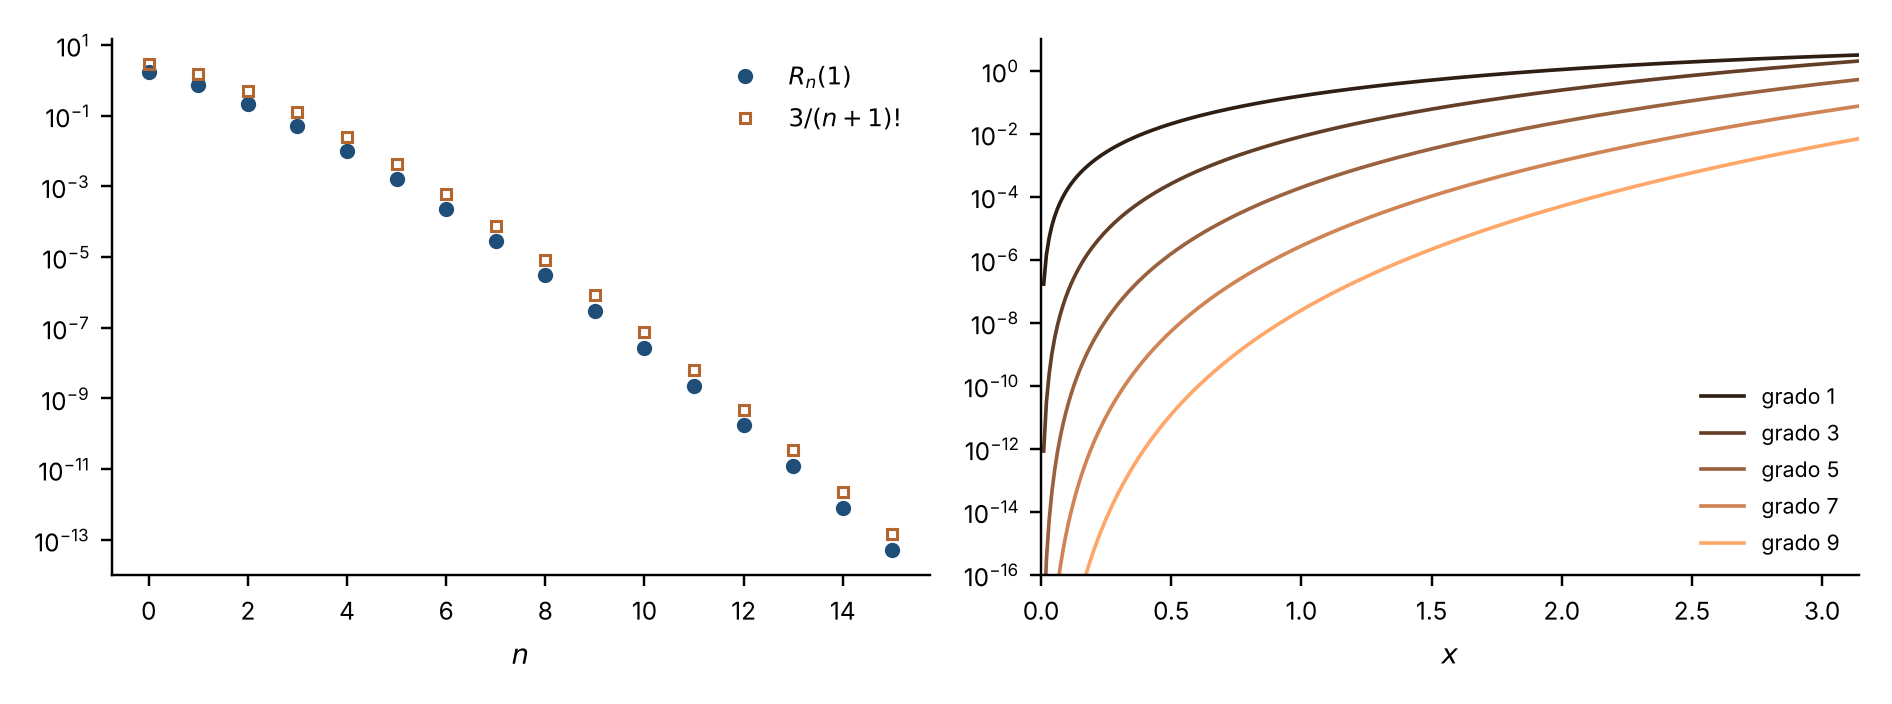
\includegraphics[width=\textwidth]{figure/errore_taylor.png}
\caption{A sinistra: l'errore $R_{n}(1)=e-\sum_{k=0}^{n}\frac1{k!}$ (punti blu) e la stima
$\frac3{(n+1)!}$ (punti rame), in scala logaritmica: la stima segue fedelmente l'errore vero.
A destra: l'errore $\abs{\sen x-T_{2n+1}(x)}$ in $[0,\pi]$ per $2n+1=1,3,5,7,9$; vicino a $0$ i
polinomi di grado alto sono straordinariamente precisi, mentre allontanandosi da $0$
l'errore cresce, pur restando sotto la stima $\frac{x^{2n+3}}{(2n+3)!}$ fornita dal resto di
Lagrange (\texttt{python/fig\_errore\_taylor.py}).}
\label{fig:errore-taylor}
\end{figure}

\begin{idea}[Come calcolano le calcolatrici]
Nessuna calcolatrice usa direttamente lo sviluppo di Taylor per $\sen x$ con $x$ grande:
la \cref{fig:errore-taylor} mostra che l'errore cresce rapidamente allontanandosi dal
centro. Si usa prima la periodicità e la simmetria per ricondurre l'argomento in un
intervallo piccolo, ad esempio $[0,\frac\pi4]$ (\emph{riduzione dell'argomento}), e poi un
polinomio di grado moderato, i cui coefficienti sono spesso leggermente modificati
rispetto a quelli di Taylor per distribuire l'errore uniformemente sull'intervallo
(polinomi di \emph{migliore approssimazione}). Un metodo diverso, che usa soltanto
somme e scorrimenti di cifre, è l'algoritmo CORDIC, ideato nel 1956 da Jack Volder alla
Convair per il calcolatore di navigazione del bombardiere B-58 e poi adottato nelle
prime calcolatrici tascabili.
\end{idea}

\subsection{L'irrazionalità del numero \texorpdfstring{$e$}{e}}

La stima \eqref{eq:stima-e} è così precisa da permettere di dimostrare che $e$ non è un
numero razionale. La dimostrazione, che risale a Fourier, è un piccolo gioiello: si
moltiplica la \eqref{eq:stima-e} per un fattoriale opportuno, in modo da rendere intero
tutto ciò che può esserlo, e si osserva che ciò che resta è un intero strettamente
compreso tra $0$ e $1$.

\begin{teorema}[Irrazionalità di $e$]\label{teo:e-irrazionale}
\index{numero di Nepero!irrazionalità}
Il numero $e$ è irrazionale.
\end{teorema}

\begin{schema}
\Ipotesi{la stima \eqref{eq:stima-e}: $0<e-\sum_{k=0}^{n}\frac1{k!}<\frac3{(n+1)!}$ per ogni $n\ge1$; \
$2<e<3$.}
\Tesi{non esistono interi $p,q\ge1$ con $e=\frac pq$.}
\end{schema}

\begin{strategia}
Ragioniamo per assurdo, supponendo $e=\frac pq$. Moltiplichiamo la \eqref{eq:stima-e}, con
$n=q$, per $q!$: il termine $q!\,e=p\,(q-1)!$ è intero, e lo è anche $q!\sum_{k=0}^{q}\frac1{k!}$, perché
ogni $k!$ con $k\le q$ divide $q!$. Allora anche $q!\,R_{q}(1)$ è un intero; ma la stima del resto
lo pone strettamente tra $0$ e $\frac3{q+1}$, che non supera $1$ se $q\ge2$. Un intero
strettamente compreso tra $0$ e $1$ non esiste.
\end{strategia}

\begin{dimostrazione}
Supponiamo per assurdo che sia $e=\frac pq$ con $p,q$ interi positivi. Poiché $2<e<3$, $e$ non è
intero, e quindi $q\ge2$. Applichiamo la \eqref{eq:stima-e} con $n=q$ e moltiplichiamo per
$q!$:
\[
  0<q!\,e-\sum_{k=0}^{q}\frac{q!}{k!}<\frac{3\,q!}{(q+1)!}=\frac3{q+1} .
\]
Il numero $q!\,e=q!\,\frac pq=p\,(q-1)!$ è intero; anche ogni $\frac{q!}{k!}=(k+1)(k+2)\cdots q$, con
$0\le k\le q$, è intero (per $k=q$ vale $1$). Dunque il numero
$N=q!\,e-\sum_{k=0}^{q}\frac{q!}{k!}$ è intero, e verifica $0<N<\frac3{q+1}\le1$, perché $q\ge2$. Ma non
esistono interi strettamente compresi tra $0$ e $1$: l'assurdo prova la tesi.
\end{dimostrazione}

\subsection{Approfondimento: una tavola dei logaritmi}
\label{subsec:tavola-logaritmi}

Il procedimento del paragrafo funziona male per il logaritmo, se si parte dallo sviluppo
di $\log(1+x)$: per $x=1$ la stima del \cref{sec:taylor-peano} dà soltanto
$\abs{R_{n}(1)}\le\frac1{n+1}$, e per avere $\log2$ con sei decimali esatti occorrerebbero milioni
di termini; per $x>1$, poi, i polinomi si allontanano dalla funzione. Giusti
\cite{giusti} suggerisce invece lo sviluppo di $\log\frac{1+x}{1-x}$, che si ottiene con lo stesso
artificio usato per l'arcotangente nella \cref{prop:sviluppo-arctg}.

\begin{proposizione}[Sviluppo di $\log\frac{1+x}{1-x}$]\label{prop:sviluppo-log-rapporto}
Per ogni intero $n\ge0$ e ogni $x\in(-1,1)$,
\begin{equation}\label{eq:sviluppo-log-rapporto}
\begin{gathered}
  \log\frac{1+x}{1-x}=2\Bigl(x+\frac{x^{3}}3+\frac{x^{5}}5+\dots+\frac{x^{2n+1}}{2n+1}\Bigr)+R(x),\\
  R(x)=2\int_{0}^{x}\frac{t^{2n+2}}{1-t^{2}}\,dt, \qquad
  \abs{R(x)}\le\frac{2\abs x^{2n+3}}{(2n+3)(1-x^{2})} ,
\end{gathered}
\end{equation}
e il resto $R(x)$ ha il segno di $x$.
\end{proposizione}

\begin{schema}
\Ipotesi{$n\ge0$ intero; \ $\abs x<1$.}
\Tesi{la \eqref{eq:sviluppo-log-rapporto}: il resto in forma integrale, la sua stima, e
$R(x)$ dello stesso segno di $x$.}
\end{schema}

\begin{strategia}
La derivata di $\log(1+x)-\log(1-x)$ è $\frac2{1-x^{2}}$, e $\frac1{1-t^{2}}$ è la somma della
progressione geometrica di ragione $t^{2}$, a meno di un resto esplicito. Integrando tra $0$
e $x$ la somma dà il polinomio, e nel resto il denominatore $1-t^{2}$ si minora con il suo
valore nell'estremo $x$.
\end{strategia}

\begin{dimostrazione}
Per $\abs t<1$, la formula della progressione geometrica (\cref{prop:geometrica}) con
ragione $t^{2}\neq1$ dà $\sum_{k=0}^{n}t^{2k}=\frac{1-t^{2n+2}}{1-t^{2}}$, cioè
\[
  \frac1{1-t^{2}}=\sum_{k=0}^{n}t^{2k}+\frac{t^{2n+2}}{1-t^{2}} .
\]
La funzione $g(x)=\log(1+x)-\log(1-x)=\log\frac{1+x}{1-x}$ è derivabile in $(-1,1)$, con
$g'(x)=\frac1{1+x}+\frac1{1-x}=\frac2{1-x^{2}}$ per la \eqref{eq:derivata-log} e la regola della catena,
e $g(0)=0$. Per la formula fondamentale (\cref{teo:formula-fondamentale}), integrando
l'uguaglianza precedente moltiplicata per $2$,
\[
  g(x)=2\int_{0}^{x}\frac{dt}{1-t^{2}}=2\sum_{k=0}^{n}\frac{x^{2k+1}}{2k+1}+R(x) .
\]
Sia $0<x<1$. Per $0\le t\le x$ si ha $1\ge1-t^{2}\ge1-x^{2}>0$, e quindi
$t^{2n+2}\le\frac{t^{2n+2}}{1-t^{2}}\le\frac{t^{2n+2}}{1-x^{2}}$; integrando tra $0$ e $x$, per il
confronto (\cref{teo:confronto-integrali}),
\[
  0<\frac{2x^{2n+3}}{2n+3}\le R(x)\le\frac{2x^{2n+3}}{(2n+3)(1-x^{2})} .
\]
Infine, poiché l'integrando è una funzione pari di $t$, la
sostituzione $t=-u$ mostra che $R(-x)=-R(x)$, e il caso $-1<x<0$ si riconduce al
precedente; per $x=0$ tutto è ovvio.
\end{dimostrazione}

La stima è tanto migliore quanto più $x$ è piccolo, e il quoziente $\frac{1+x}{1-x}$ assume
valori comodi se $x=\frac1{2N+1}$, con $N\in\N$: allora $\frac{1+x}{1-x}=\frac{2N+2}{2N}=\frac{N+1}N$ e
$1-x^{2}=\frac{4N(N+1)}{(2N+1)^{2}}$, sicché
\begin{equation}\label{eq:log-N}
\begin{gathered}
  \log\frac{N+1}N=2\sum_{k=0}^{n}\frac1{(2k+1)\,(2N+1)^{2k+1}}+R, \\
  0<R\le\frac1{2N(N+1)\,(2n+3)\,(2N+1)^{2n+1}} .
\end{gathered}
\end{equation}
Con $N=1$, cioè $x=\frac13$, si ottiene $\log2$: quattro termini ($n=3$) danno
\[
  \log2\simeq2\Bigl(\frac13+\frac1{81}+\frac1{1215}+\frac1{15\,309}\Bigr)=\frac{53\,056}{76\,545}=0{,}6931347\ldots ,
\]
con un errore positivo e inferiore a $\frac1{4\cdot9\cdot3^{7}}=\frac1{78\,732}<1{,}3\cdot10^{-5}$: dunque
$0{,}693134<\log2<0{,}693148$, e $\log2=0{,}6931\ldots$ con quattro decimali esatti; con lo
sviluppo di $\log(1+x)$, per garantire lo stesso errore, la stima richiederebbe quasi
ottantamila termini. Noto $\log2$, si calcolano
$\log3=\log2+\log\frac32$ (con $N=2$), $\log5=2\log2+\log\frac54$ (con $N=4$),
$\log7=\log2+\log3+\log\frac76$ (con $N=6$), e in generale il logaritmo di un primo $p$ dispari
da quelli dei primi minori, perché $p-1$ si scompone in essi, aggiungendo $\log\frac p{p-1}$
con $N=p-1$. Al crescere di $N$ la convergenza diventa sempre più rapida, e i
logaritmi dei primi successivi richiedono pochi termini. Per la proprietà $\log(ab)=\log a+\log b$, dai
logaritmi dei primi si ottengono per somma quelli di tutti gli interi, e dividendo per
$\log10=\log2+\log5$ i logaritmi decimali di Briggs, di cui parla la nota storica che
segue. Il programma costruisce questa piccola tavola con un errore garantito inferiore a
$10^{-13}$ per ciascun termine $\log\frac{N+1}N$, e la confronta con la libreria \texttt{math}.

\needspace{10\baselineskip}
\begin{python}[Una tavola dei logaritmi con errore garantito]
import math
from fractions import Fraction as F

def logN(N, tol=F(1, 10**13)):
    """log((N+1)/N) con x = 1/(2N+1), errore garantito < tol."""
    n = 0
    while F(1, 2*N*(N+1)*(2*n+3)*(2*N+1)**(2*n+1)) >= tol:
        n += 1
    x = F(1, 2*N + 1)
    T = 2 * sum(x**(2*k + 1) / (2*k + 1) for k in range(n + 1))
    return T, n + 1                  # valore e numero di termini

l2, t1 = logN(1)                     # log 2
l32, t2 = logN(2)                    # log 3/2
l54, t4 = logN(4)                    # log 5/4
l76, t6 = logN(6)                    # log 7/6
print("termini per N = 1, 2, 4, 6:", t1, t2, t4, t6)
tavola = {2: l2, 3: l2 + l32, 5: 2*l2 + l54}
tavola[7] = tavola[2] + tavola[3] + l76
for p, v in tavola.items():
    print(f"log {p} = {float(v):.12f}   (math.log: "
          f"{math.log(p):.12f})")
l10 = tavola[2] + tavola[5]
print(f"log10(2) = {float(tavola[2] / l10):.12f}")
\end{python}
\begin{risultato}
termini per N = 1, 2, 4, 6: 13 9 6 6
log 2 = 0.693147180560   (math.log: 0.693147180560)
log 3 = 1.098612288668   (math.log: 1.098612288668)
log 5 = 1.609437912434   (math.log: 1.609437912434)
log 7 = 1.945910149055   (math.log: 1.945910149055)
log10(2) = 0.301029995664
\end{risultato}

Per $N=1$ servono tredici termini, per $N=4$ e $N=6$ ne bastano sei. Gli errori dei
singoli termini si sommano, ma restano dell'ordine di $10^{-13}$: le dodici cifre decimali
stampate coincidono con quelle della libreria. Il valore $\log_{10}2=0{,}30103\ldots$ è quello
che si legge in ogni tavola dei logaritmi decimali.

\begin{notastorica}[Tavole e irrazionalità]
Le prime tavole dei logaritmi furono pubblicate da John Napier nel 1614 (\emph{Mirifici
logarithmorum canonis descriptio}); nel 1624 Henry Briggs pubblicò l'\emph{Arithmetica
logarithmica}, con i logaritmi decimali degli interi da $1$ a $20\,000$ e da $90\,000$ a
$100\,000$, calcolati con quattordici cifre. Quei calcoli, eseguiti a mano con metodi
ingegnosi ma faticosissimi, precedono di decenni la scoperta degli sviluppi in serie.
In seguito le serie fornirono i valori «di appoggio» con grande precisione, come
abbiamo fatto nel \S\ref{subsec:tavola-logaritmi}, mentre il
resto della tavola si completava per interpolazione con il metodo delle differenze
finite: così furono calcolate le grandi tavole francesi dirette da Gaspard de Prony
negli anni Novanta del Settecento, e lo stesso metodo ispirò la macchina alle differenze
di Charles Babbage. Le tavole furono lo strumento quotidiano di astronomi, navigatori e
ingegneri fino all'avvento delle calcolatrici elettroniche. L'irrazionalità
di $e$ fu dimostrata da Eulero nel 1737, mediante lo sviluppo in frazione continua; la
dimostrazione qui riportata, dovuta a Fourier, fu pubblicata nel 1815. Che $e$ sia
addirittura \emph{trascendente}, cioè non sia radice di alcun polinomio a coefficienti
interi, fu dimostrato da Charles Hermite nel 1873.
\end{notastorica}

%% ----------------------------------------------------------------------------
%%  §10.6  Esercizi di riepilogo
%% ----------------------------------------------------------------------------
\section{Esercizi di riepilogo}
\label{sec:esercizi-cap10}

Come nei capitoli precedenti, ogni soluzione è accompagnata da una nota sulla
\emph{scelta logica} che la guida.

\needspace{8\baselineskip}
\subsection*{Sviluppi di Taylor}

\begin{esercizio}[La formula di Machin]\label{es:machin}
Verificare la formula di Machin \eqref{eq:machin}:
$\frac\pi4=4\operatorname{arctg}\frac15-\operatorname{arctg}\frac1{239}$.
\begin{soluzione}
Dividendo le formule di addizione \eqref{eq:addizione-sen} e \eqref{eq:addizione-cos} per
$\cos\alpha\cos\beta$ si ottiene $\tg(\alpha\pm\beta)=\frac{\tg\alpha\pm\tg\beta}{1\mp\tg\alpha\,\tg\beta}$. Sia $\alpha=\operatorname{arctg}\frac15$.
Allora
\[
\begin{gathered}
  \tg2\alpha=\frac{2/5}{1-1/25}=\frac5{12}, \qquad
  \tg4\alpha=\frac{2\cdot5/12}{1-25/144}=\frac{120}{119},\\
  \tg\Bigl(4\alpha-\frac\pi4\Bigr)=\frac{\frac{120}{119}-1}{1+\frac{120}{119}}=\frac1{239} .
\end{gathered}
\]
Poiché $0<\alpha<\frac15$ (si ha $\operatorname{arctg}x<x$ per $x>0$: per la \eqref{eq:sviluppo-arctg}
con $n=0$, il resto $R(x)=-\int_{0}^{x}\frac{t^{2}}{1+t^{2}}\,dt$ è negativo), risulta
$-\frac\pi4<4\alpha-\frac\pi4<\frac45-\frac\pi4<\frac\pi2$; in $(-\frac\pi2,\frac\pi2)$ la tangente è invertibile, e
quindi $4\alpha-\frac\pi4=\operatorname{arctg}\frac1{239}$. \emph{Scelta logica:} un'identità tra
arcotangenti si dimostra calcolando la tangente di entrambi i membri; ma la tangente non
è iniettiva, ed è indispensabile controllare che gli angoli cadano nell'intervallo in cui
essa è invertibile.
\end{soluzione}
\end{esercizio}

\begin{esercizio}\label{es:sviluppo-tangente}
Determinare il polinomio di Taylor di ordine $5$ della funzione $\tg x$ in $x_{0}=0$.
\begin{soluzione}
La funzione $\tg x$ è derivabile infinite volte in $(-\frac\pi2,\frac\pi2)$ ed è dispari; le sue
derivate di ordine pari sono dispari, e quindi nulle in $0$. Il polinomio cercato ha
dunque la forma $x+a_{3}x^{3}+a_{5}x^{5}$ (il coefficiente di $x$ è $\tg'(0)=1$), e
$\tg x=x+a_{3}x^{3}+a_{5}x^{5}+o(x^{5})$. Moltiplicando per
$\cos x=1-\frac{x^{2}}2+\frac{x^{4}}{24}+o(x^{5})$ e usando le regole della \cref{prop:algebra-o},
\[
  \sen x=\tg x\cos x=x+\Bigl(a_{3}-\frac12\Bigr)x^{3}+\Bigl(a_{5}-\frac{a_{3}}2+\frac1{24}\Bigr)x^{5}+o(x^{5}) .
\]
Per l'unicità del polinomio di Taylor (\cref{prop:unicita-taylor}) i coefficienti devono
coincidere con quelli di $\sen x=x-\frac{x^{3}}6+\frac{x^{5}}{120}+o(x^{5})$: $a_{3}-\frac12=-\frac16$, cioè
$a_{3}=\frac13$, e $a_{5}=\frac1{120}+\frac16-\frac1{24}=\frac2{15}$. Dunque
\[
  \tg x=x+\frac{x^{3}}3+\frac{2x^{5}}{15}+o(x^{6}) ,
\]
dove il resto è $o(x^{6})$ perché anche il coefficiente di $x^{6}$ è nullo.
\emph{Scelta logica:} invece di calcolare cinque derivate della tangente, sempre più complicate, si
usa la relazione $\sen x=\tg x\cos x$ tra funzioni di cui conosciamo gli sviluppi, e
l'unicità permette di identificare i coefficienti (\emph{metodo dei coefficienti
indeterminati}).
\end{soluzione}
\end{esercizio}

\begin{esercizio}
Determinare lo sviluppo di Mac Laurin di ordine $5$ di $\arcsen x$.
\begin{soluzione}
Per la \eqref{eq:derivata-arcsen}, $D\arcsen x=(1-x^{2})^{-1/2}$. Dalla \eqref{eq:taylor-potenza}
con $b=-\frac12$, $(1+u)^{-1/2}=1-\frac u2+\frac38\,u^{2}+o(u^{2})$, e con $u=-t^{2}$ (\cref{lem:sostituzione-o})
\[
  \frac1{\sqrt{1-t^{2}}}=1+\frac{t^{2}}2+\frac38\,t^{4}+o(t^{4}) .
\]
Integrando termine a termine tra $0$ e $x$, per la \eqref{eq:integrazione-termine} e poiché
$\arcsen0=0$,
\[
  \arcsen x=x+\frac{x^{3}}6+\frac3{40}\,x^{5}+o(x^{5}) .
\]
\emph{Scelta logica:} come per l'arcotangente, si sviluppa la derivata, che è una
potenza di un binomio, e si integra; il \cref{lem:integrazione-o} garantisce che il resto
integrato è ancora trascurabile, con un ordine in più.
\end{soluzione}
\end{esercizio}

\begin{esercizio}\label{es:derivata-decima}
Sia $f(x)=\sen(x^{2})$. Calcolare $f^{(9)}(0)$ e $f^{(10)}(0)$.
\begin{soluzione}
Dalla \eqref{eq:taylor-sen} con $n=2$ e la sostituzione $t=x^{2}$,
\[
  \sen(x^{2})=x^{2}-\frac{x^{6}}6+\frac{x^{10}}{120}+o(x^{12}) .
\]
Il polinomio a secondo membro, di grado $10$, approssima $f$ con un errore $o(x^{10})$; per
l'unicità è il polinomio di Taylor di ordine $10$, il cui coefficiente di $x^{k}$ è
$\frac{f^{(k)}(0)}{k!}$. Dunque $f^{(9)}(0)=0$ e $\frac{f^{(10)}(0)}{10!}=\frac1{120}$, cioè
$f^{(10)}(0)=\frac{3\,628\,800}{120}=30\,240$. \emph{Scelta logica:} calcolare dieci derivate di
$\sen(x^{2})$ sarebbe proibitivo; l'unicità del polinomio di Taylor permette di leggere le
derivate nei coefficienti di uno sviluppo ottenuto per sostituzione.
\end{soluzione}
\end{esercizio}

\needspace{8\baselineskip}
\subsection*{Limiti e parti principali}

\begin{esercizio}
Calcolare (a) $\displaystyle\lim_{x\to0}\frac{\log(1+x)-\sen x}{x^{2}}$; \
(b) $\displaystyle\lim_{x\to0}\frac{e^{x^{2}}-\cos x-\frac32x^{2}}{x^{4}}$; \
(c) $\displaystyle\lim_{x\to0}\frac{\tg x-\sen x}{x^{3}}$.
\begin{soluzione}
(a) Il denominatore ha ordine $2$: basta sviluppare al secondo ordine.
$\log(1+x)=x-\frac{x^{2}}2+o(x^{2})$ e $\sen x=x+o(x^{2})$, dunque il numeratore è
$-\frac{x^{2}}2+o(x^{2})$ e il limite vale $-\frac12$.

(b) Occorre il quarto ordine. Con $t=x^{2}$ nello sviluppo dell'esponenziale,
$e^{x^{2}}=1+x^{2}+\frac{x^{4}}2+o(x^{4})$; inoltre $\cos x=1-\frac{x^{2}}2+\frac{x^{4}}{24}+o(x^{5})$. Il
numeratore è
$x^{2}+\frac{x^{2}}2-\frac32\,x^{2}+\bigl(\frac12-\frac1{24}\bigr)x^{4}+o(x^{4})=\frac{11}{24}\,x^{4}+o(x^{4})$, e il
limite vale $\frac{11}{24}$.

(c) Per l'\cref{es:sviluppo-tangente}, $\tg x-\sen x=\frac{x^{3}}3+\frac{x^{3}}6+o(x^{4})=\frac{x^{3}}2+o(x^{4})$, e
il limite vale $\frac12$.

\emph{Scelta logica:} l'ordine dello sviluppo è dettato dal denominatore (la sua parte
principale); se i termini del numeratore si elidono fino a quell'ordine, il limite è
zero, altrimenti la \cref{prop:parte-principale} lo fornisce subito.
\end{soluzione}
\end{esercizio}

\begin{esercizio}
Calcolare $\displaystyle\lim_{n\to+\infty}n^{2}\Bigl(1-n\sen\frac1n\Bigr)$.
\begin{soluzione}
Con $x=\frac1n\to0$ il limite è quello di $\frac{1}{x^{2}}\bigl(1-\frac{\sen x}x\bigr)=\frac{x-\sen x}{x^{3}}$. Poiché
$x-\sen x=\frac{x^{3}}6+o(x^{4})$, il limite vale $\frac16$. \emph{Scelta logica:} un limite di
successione che contiene $\frac1n$ in funzioni elementari si riconduce, mediante la
definizione di limite con le successioni, a un limite di funzione per $x\to0$, dove gli
sviluppi di Taylor sono disponibili.
\end{soluzione}
\end{esercizio}

\begin{esercizio}\label{es:verifica-19-30}
Determinare la parte principale, per $x\to0$, di $N(x)=3x^{3}-3x\cos x+\sen3x$, e
dedurre che la funzione dell'\cref{es:limite-taylor-2} è un infinitesimo equivalente a
$\frac{19}{30}\,x$.
\begin{soluzione}
Nell'\cref{es:limite-taylor-2} gli sviluppi fino all'ordine $4$ hanno dato $N(x)=o(x^{4})$.
Aggiungiamo un termine: $\cos x=1-\frac{x^{2}}2+\frac{x^{4}}{24}+o(x^{5})$, quindi
$3x\cos x=3x-\frac32x^{3}+\frac18x^{5}+o(x^{6})$, e
$\sen3x=3x-\frac92x^{3}+\frac{243}{120}x^{5}+o(x^{6})$. Allora
\[
  N(x)=\Bigl(-\frac18+\frac{81}{40}\Bigr)x^{5}+o(x^{6})=\frac{19}{10}\,x^{5}+o(x^{6}) .
\]
Per la \cref{prop:parte-principale} con $p=5$, $q=4$, la funzione $\frac{N(x)}{3x^{4}}$ è
$\frac{19}{30}\,x\,(1+o(1))$. \emph{Scelta logica:} quando tutti i termini fino a un certo ordine si
elidono, il limite è zero; per sapere \emph{come} la funzione tende a zero occorre
spingere lo sviluppo fino al primo termine superstite.
\end{soluzione}
\end{esercizio}

\begin{esercizio}
Determinare l'ordine di infinitesimo e la parte principale di $f(x)=\sen x-x\cos x$ per
$x\to0$, e calcolare $\displaystyle\lim_{x\to0}\frac{\sen x-x\cos x}{x-\sen x}$.
\begin{soluzione}
$\sen x=x-\frac{x^{3}}6+o(x^{4})$ e $x\cos x=x-\frac{x^{3}}2+o(x^{4})$, dunque
$f(x)=\frac{x^{3}}3+o(x^{4})$: $f$ è un infinitesimo di ordine $3$ con parte principale $\frac{x^{3}}3$.
Poiché $x-\sen x=\frac{x^{3}}6+o(x^{4})$, per la \cref{prop:parte-principale} il limite vale
$\frac{1/3}{1/6}=2$. \emph{Scelta logica:} con il teorema di L'Hôpital occorrerebbero più
applicazioni successive, con derivate sempre più lunghe; con gli sviluppi bastano due
righe.
\end{soluzione}
\end{esercizio}

\needspace{8\baselineskip}
\subsection*{Resto e stime}

\begin{esercizio}\label{es:log-disuguaglianza}
Dimostrare che per ogni $x>0$ si ha $x-\frac{x^{2}}2<\log(1+x)<x$.
\begin{soluzione}
Sia $f(x)=\log(1+x)$: $f'(x)=\frac1{1+x}$, $f''(x)=-\frac1{(1+x)^{2}}$, $f'''(x)=\frac2{(1+x)^{3}}$. Per il
\cref{teo:resto-lagrange-generale}, applicato in $(-1,+\infty)$ con $x_{0}=0$, esistono
$x_{1},x_{2}\in(0,x)$ tali che
\[
\begin{aligned}
  \log(1+x)&=x-\frac{x^{2}}{2(1+x_{1})^{2}}<x,\\
  \log(1+x)&=x-\frac{x^{2}}2+\frac{x^{3}}{3(1+x_{2})^{3}}>x-\frac{x^{2}}2 .
\end{aligned}
\]
\emph{Scelta logica:} quando la derivata $f^{(n+1)}$ ha segno costante, il resto di
Lagrange ha segno noto, e la formula di Taylor diventa una disuguaglianza.
\end{soluzione}
\end{esercizio}

\begin{esercizio}
Calcolare $\sqrt{1{,}1}$ con un errore inferiore a $10^{-4}$.
\begin{soluzione}
Sia $f(x)=\sqrt{1+x}$, $x_{0}=0$, $x=\frac1{10}$. Le derivate sono
$f'=\frac12(1+x)^{-1/2}$, $f''=-\frac14(1+x)^{-3/2}$, $f'''=\frac38(1+x)^{-5/2}$. Con $n=1$ la stima
\eqref{eq:stima-resto} dà $\abs{R_{1}}\le\frac14\cdot\frac{10^{-2}}2=1{,}25\cdot10^{-3}$, insufficiente. Con
$n=2$, poiché $0<f'''\le\frac38$ in $[0,\frac1{10}]$,
\[
  0<R_{2}\Bigl(\frac1{10}\Bigr)\le\frac38\cdot\frac{10^{-3}}{6}=6{,}25\cdot10^{-5}<10^{-4} ,
\]
e $T_{2}(\frac1{10})=1+\frac1{20}-\frac1{800}=1{,}04875$. Dunque
$1{,}04875<\sqrt{1{,}1}\le1{,}0488125$ (il valore esatto è $1{,}0488088\ldots$).
\emph{Scelta logica:} si aumenta $n$ finché la stima del resto scende sotto la precisione richiesta;
il segno di $f'''$ dice inoltre da che parte sta l'errore.
\end{soluzione}
\end{esercizio}

\begin{esercizio}[L'integrale della campana di Gauss]\label{es:integrale-gauss-taylor}
Calcolare $\int_{0}^{1}e^{-x^{2}}\,dx$ con un errore inferiore a $10^{-5}$, e confrontare il risultato
con le stime dell'\cref{es:stima-gaussiana}.
\begin{soluzione}
Per il \cref{teo:resto-lagrange} applicato a $g(t)=e^{-t}$ con centro $0$, per ogni $t>0$
esiste $\tau\in(0,t)$ tale che
\[
  e^{-t}=\sum_{k=0}^{n}\frac{(-t)^{k}}{k!}+R_{n}(t), \qquad R_{n}(t)=(-1)^{n+1}\frac{e^{-\tau}}{(n+1)!}\,t^{n+1} ;
\]
dunque $\abs{R_{n}(t)}\le\frac{t^{n+1}}{(n+1)!}$, e $R_{n}(t)$ ha il segno di $(-1)^{n+1}$. Con $t=x^{2}$ la
funzione $R_{n}(x^{2})$, differenza di funzioni continue, è integrabile in $[0,1]$, e per
la linearità e il confronto (\cref{teo:confronto-integrali,teo:valore-assoluto})
\[
\begin{gathered}
  \int_{0}^{1}e^{-x^{2}}dx=\sum_{k=0}^{n}\frac{(-1)^{k}}{k!\,(2k+1)}+E_{n},\\
  \abs{E_{n}}\le\int_{0}^{1}\frac{x^{2n+2}}{(n+1)!}\,dx=\frac1{(n+1)!\,(2n+3)} .
\end{gathered}
\]
Per $n=6$ la stima vale $\frac1{75\,600}\approx1{,}3\cdot10^{-5}$, insufficiente; per $n=7$ vale
$\frac1{685\,440}<1{,}5\cdot10^{-6}$, e inoltre $E_{7}\ge0$, perché $R_{7}\ge0$. Dunque
\[
\begin{aligned}
  \int_{0}^{1}e^{-x^{2}}dx&\simeq1-\frac13+\frac1{10}-\frac1{42}+\frac1{216}-\frac1{1320}
  +\frac1{9360}-\frac1{75\,600}\\
  &=0{,}7468228\ldots
\end{aligned}
\]
per difetto, con un errore inferiore a $1{,}5\cdot10^{-6}$: $0{,}7468228<\int_{0}^{1}e^{-x^{2}}dx<0{,}7468243$.
Otto termini bastano dove le somme integrali dell'\cref{es:stima-gaussiana}, con
$10\,000$ suddivisioni, lasciano un'incertezza di $6\cdot10^{-5}$. \emph{Scelta logica:} se la
funzione integranda non ha una primitiva elementare, la si sostituisce con un polinomio
di Taylor, che si integra esattamente; la stima del resto, integrata, certifica
l'errore.
\end{soluzione}
\end{esercizio}

\begin{esercizio}[Freccia dell'ala con portanza ellittica]\label{es:freccia-ellittica}
Con le notazioni del \cref{sec:applicazioni-integrali} e della \cref{prop:freccia}, sia
$T(y)=\int_{y}^{s}l$ il taglio (da non confondere con un polinomio di Taylor). Dimostrare
che
\[
  \int_{0}^{s}(s-t)M(t)\,dt=\frac{s^{2}}2M(0)-\frac{s^{3}}6T(0)+\frac16\int_{0}^{s}(s-t)^{3}l(t)\,dt ,
\]
e dedurne che per la distribuzione ellittica $l(y)=l_{0}\sqrt{1-(y/s)^{2}}$ la freccia
all'estremità vale $v(s)=\frac{l_{0}s^{4}}{EI}\bigl(\frac\pi{32}-\frac1{45}\bigr)$, cioè
$1-\frac{32}{45\pi}\approx0{,}774$ volte quella dovuta a un carico uniforme con la stessa portanza
totale.
\begin{soluzione}
Si integra per parti due volte, usando $M'=-T$, $T'=-l$ e $M(s)=T(s)=0$
(\cref{prop:taglio-momento}). Con la primitiva $-\frac{(s-t)^{2}}2$ di $s-t$,
\[
\begin{aligned}
  \int_{0}^{s}(s-t)M\,dt&=\Bigl[-\frac{(s-t)^{2}}2M\Bigr]_{0}^{s}-\int_{0}^{s}\frac{(s-t)^{2}}2\,T\,dt\\
  &=\frac{s^{2}}2M(0)-\int_{0}^{s}\frac{(s-t)^{2}}2\,T\,dt ;
\end{aligned}
\]
con la primitiva $-\frac{(s-t)^{3}}6$ di $\frac{(s-t)^{2}}2$,
$\int_{0}^{s}\frac{(s-t)^{2}}2T\,dt=\frac{s^{3}}6T(0)-\frac16\int_{0}^{s}(s-t)^{3}l\,dt$, e la formula segue.
Per la distribuzione ellittica, dall'\cref{es:taglio-ellittico}, $M(0)=\frac{l_{0}s^{2}}3$ e
$T(0)=\frac\pi4l_{0}s$; con $t=sw$,
$\int_{0}^{s}(s-t)^{3}l\,dt=l_{0}s^{4}\int_{0}^{1}(1-w)^{3}\sqrt{1-w^{2}}\,dw$. Sviluppando il cubo e usando
\[
\begin{gathered}
  \int_{0}^{1}\!\sqrt{1-w^{2}}\,dw=\frac\pi4, \qquad \int_{0}^{1}\!w\sqrt{1-w^{2}}\,dw=\frac13,\\
  \int_{0}^{1}\!w^{2}\sqrt{1-w^{2}}\,dw=\frac\pi{16}, \qquad \int_{0}^{1}\!w^{3}\sqrt{1-w^{2}}\,dw=\frac2{15}
\end{gathered}
\]
(il secondo e il quarto con $u=1-w^{2}$, il terzo con $w=\sen\theta$), si trova
$\int_{0}^{1}(1-w)^{3}\sqrt{1-w^{2}}\,dw=\frac\pi4-1+\frac{3\pi}{16}-\frac2{15}=\frac{7\pi}{16}-\frac{17}{15}$. Allora
\[
  EI\,v(s)=l_{0}s^{4}\Bigl[\frac16-\frac\pi{24}+\frac16\Bigl(\frac{7\pi}{16}-\frac{17}{15}\Bigr)\Bigr]
  =l_{0}s^{4}\Bigl(\frac\pi{32}-\frac1{45}\Bigr) .
\]
Con $l_{0}=\frac4\pi\cdot\frac Wb$ e, per il carico uniforme $l=\frac Wb$, $EI\,v(s)=\frac{W}{b}\frac{s^{4}}8$, il
rapporto è $\frac{32}\pi\bigl(\frac\pi{32}-\frac1{45}\bigr)=1-\frac{32}{45\pi}\approx0{,}7736$, in accordo con il
calcolo numerico del \cref{sec:resto-integrale}. \emph{Scelta logica:} ogni integrazione
per parti trasferisce una derivata dal peso polinomiale alle grandezze della trave,
scendendo da $M$ a $T$ e da $T$ al carico $l$, che è noto esplicitamente; i termini di
bordo all'estremità libera si annullano perché lì taglio e momento sono nulli.
\end{soluzione}
\end{esercizio}

\needspace{8\baselineskip}
\subsection*{Taylor e calcolo numerico}

\begin{esercizio}[L'errore delle differenze finite]\label{es:errore-differenze}
Sia $f$ di classe $C^{3}$ in un intervallo contenente $[x-h,x+h]$, con $h>0$, e siano
$M_{2}$ e $M_{3}$ i massimi di $\abs{f''}$ e di $\abs{f'''}$ in quell'intervallo. Dimostrare che
\[
\begin{aligned}
  \Bigl|\frac{f(x+h)-f(x)}h-f'(x)\Bigr|&\le\frac{M_{2}}2\,h ,\\
  \Bigl|\frac{f(x+h)-f(x-h)}{2h}-f'(x)\Bigr|&\le\frac{M_{3}}6\,h^{2} .
\end{aligned}
\]
\begin{soluzione}
Per il \cref{teo:resto-lagrange} con $n=1$, $f(x+h)=f(x)+f'(x)h+\frac{f''(\xi)}2h^{2}$ con $\xi$
tra $x$ e $x+h$: dividendo per $h$ si ottiene la prima stima. Con $n=2$,
\[
  f(x\pm h)=f(x)\pm f'(x)h+\frac{f''(x)}2h^{2}\pm\frac{f'''(\xi_{\pm})}6h^{3} ,
\]
con $\xi_{+}\in(x,x+h)$ e $\xi_{-}\in(x-h,x)$. Sottraendo, i termini con $f(x)$ e con $f''(x)$ si
elidono:
\[
  \frac{f(x+h)-f(x-h)}{2h}-f'(x)=\frac{f'''(\xi_{+})+f'''(\xi_{-})}{12}\,h^{2} ,
\]
che in valore assoluto non supera $\frac{2M_{3}}{12}h^{2}=\frac{M_{3}}6h^{2}$. Sono le leggi osservate
numericamente nel \cref{cap:derivate}: dividendo $h$ per $10$, l'errore della differenza in
avanti si divide per $10$, quello della differenza centrata per $100$. \emph{Scelta
logica:} la simmetria della differenza centrata fa elidere il termine di secondo ordine;
per vederlo basta scrivere la formula di Taylor nei due punti $x\pm h$ e sottrarre.
\end{soluzione}
\end{esercizio}

\begin{esercizio}[La convergenza quadratica del metodo di Newton]\label{es:newton-quadratico}
Sia $f$ di classe $C^{2}$ in un intervallo $I$ contenente una radice $r$ di $f$, con $f'\neq0$
in $I$, e sia $x_{n+1}=x_{n}-\frac{f(x_{n})}{f'(x_{n})}$ la successione del metodo di Newton
(\cref{es:newton}). Dimostrare che, se $x_{n}\in I$, esiste $\xi$ tra $x_{n}$ e $r$ tale che
\[
  x_{n+1}-r=\frac{f''(\xi)}{2f'(x_{n})}\,(x_{n}-r)^{2} ,
\]
e dedurne che, se $\abs{f''}\le M_{2}$ e $\abs{f'}\ge m_{1}>0$ in $I$, l'errore verifica
$\abs{x_{n+1}-r}\le\frac{M_{2}}{2m_{1}}\abs{x_{n}-r}^{2}$.
\begin{soluzione}
Per il \cref{teo:resto-lagrange} con centro $x_{n}$, calcolato in $r$,
$0=f(r)=f(x_{n})+f'(x_{n})(r-x_{n})+\frac{f''(\xi)}2(r-x_{n})^{2}$. Dividendo per $f'(x_{n})$ e
ricordando che $\frac{f(x_{n})}{f'(x_{n})}=x_{n}-x_{n+1}$,
\[
  0=x_{n}-x_{n+1}+r-x_{n}+\frac{f''(\xi)}{2f'(x_{n})}(r-x_{n})^{2} ,
\]
che è la tesi. La stima segue maggiorando $\abs{f''(\xi)}$ con $M_{2}$ e minorando $\abs{f'(x_{n})}$
con $m_{1}$. Se l'errore è dell'ordine di $10^{-k}$, al passo successivo è dell'ordine di
$10^{-2k}$ (a meno della costante $\frac{M_{2}}{2m_{1}}$): il numero di cifre esatte all'incirca
raddoppia a ogni iterazione, come si era osservato nel \cref{cap:derivate}. \emph{Scelta
logica:} l'errore del metodo di Newton è il resto della formula di Taylor di ordine $1$,
perché il metodo sostituisce $f$ con la sua retta tangente; il resto di Lagrange lo
rende esplicito.
\end{soluzione}
\end{esercizio}

\needspace{8\baselineskip}
\subsection*{Applicazioni aeronautiche}

\begin{esercizio}[Arco e corda di cerchio massimo]
Due aeroporti distano $s=1000$~km lungo un cerchio massimo della Terra ($R=6371$~km).
Stimare di quanto la corda che li congiunge (la distanza in linea retta) è più corta
dell'arco, e controllare l'errore della stima.
\begin{soluzione}
L'angolo al centro è $\frac sR$, e la corda vale $2R\sen\frac s{2R}$. Posto $u=\frac s{2R}$, la
differenza è $s-2R\sen u=2R(u-\sen u)$. Per il \cref{teo:resto-lagrange} con $n=4$
($T_{4}(u)=u-\frac{u^{3}}6$, e $\abs{\sen^{(5)}}=\abs{\cos}\le1$),
$u-\sen u=\frac{u^{3}}6-R_{4}(u)$ con $\abs{R_{4}(u)}\le\frac{u^{5}}{120}$. Dunque
\[
  s-2R\sen\frac s{2R}=\frac{s^{3}}{24R^{2}}+E, \qquad
  \abs E\le2R\,\frac{u^{5}}{120}=\frac{s^{5}}{1920R^{4}} .
\]
Numericamente $\frac{s^{3}}{24R^{2}}\approx1{,}0265$~km e $\abs E\le3{,}2\cdot10^{-4}$~km: la corda è più corta
dell'arco di circa $1026$~m, con un'incertezza di qualche decimetro.
\emph{Scelta logica:} la differenza di due quantità quasi uguali si calcola sviluppando,
in modo che la cancellazione avvenga «sulla carta» e non nel calcolo numerico; il resto
di Lagrange certifica l'accuratezza della stima.
\end{soluzione}
\end{esercizio}

\begin{esercizio}[L'orizzonte, al secondo ordine]\label{es:orizzonte-secondo-ordine}
Con le notazioni del riquadro sulla distanza dell'orizzonte (\cref{sec:taylor-peano}),
dimostrare che per $h\to0$
\[
  d=R\arccos\frac R{R+h}=\sqrt{2Rh}\,\Bigl(1-\frac{5h}{12R}+o(h)\Bigr) ,
\]
e spiegare la colonna «differenza» della tabella prodotta dal programma.
\begin{soluzione}
Posto $\varepsilon=\frac hR$, l'angolo $\vartheta$ verifica $\cos\vartheta=\frac1{1+\varepsilon}$, e quindi
$1-\cos\vartheta=\frac\varepsilon{1+\varepsilon}=\varepsilon-\varepsilon^{2}+o(\varepsilon^{2})$. D'altra parte
$1-\cos\vartheta=\frac{\vartheta^{2}}2-\frac{\vartheta^{4}}{24}+o(\vartheta^{5})$. Al primo ordine si trova
$\vartheta^{2}=2\varepsilon+o(\varepsilon)$, dunque $\vartheta^{4}=4\varepsilon^{2}+o(\varepsilon^{2})$ e, poiché
$\frac{\vartheta^{5}}{\varepsilon^{2}}\to0$, anche $o(\vartheta^{5})=o(\varepsilon^{2})$. Allora
\[
  \frac{\vartheta^{2}}2=\varepsilon-\varepsilon^{2}+\frac{\varepsilon^{2}}6+o(\varepsilon^{2}) ,
  \qquad\text{cioè}\qquad
  \vartheta^{2}=2\varepsilon\Bigl(1-\frac56\,\varepsilon+o(\varepsilon)\Bigr) ,
\]
e, con lo sviluppo $(1+u)^{1/2}=1+\frac u2+o(u)$, $\vartheta=\sqrt{2\varepsilon}\,\bigl(1-\frac5{12}\,\varepsilon+o(\varepsilon)\bigr)$.
Moltiplicando per $R$ si ottiene la tesi. L'approssimazione $\sqrt{2Rh}$ \emph{sovrastima}
dunque la distanza, di circa $\sqrt{2Rh}\,\frac{5h}{12R}$: per $h=10$~km sono
$356{,}96\cdot\frac{50}{76\,452}\approx0{,}233$~km, proprio la differenza calcolata dal programma.
\emph{Scelta logica:} per conoscere l'errore di un'approssimazione «al primo ordine» si
spinge lo sviluppo all'ordine successivo; qui l'incognita $\vartheta$ compare in uno
sviluppo, e la si ricava per approssimazioni successive.
\end{soluzione}
\end{esercizio}

\begin{esercizio}[La correzione di compressibilità del tubo di Pitot]
\label{es:compressibilita}
In un flusso subsonico di un gas perfetto con $\gamma=1{,}4$, la pressione totale $p_{0}$
misurata dal tubo di Pitot e la pressione statica $p$ sono legate al numero di Mach $M$
dalla relazione isentropica $\frac{p_{0}}p=\bigl(1+\frac{\gamma-1}2M^{2}\bigr)^{\gamma/(\gamma-1)}=\bigl(1+\frac{M^{2}}5\bigr)^{7/2}$,
mentre la pressione dinamica vale $q=\frac\gamma2pM^{2}=0{,}7\,pM^{2}$. Dimostrare che
\[
  \frac{p_{0}-p}{q}=1+\frac{M^{2}}4+\frac{M^{4}}{40}+o(M^{4}) \qquad (M\to0) ,
\]
e valutare l'errore che si commette usando l'equazione di Bernoulli incomprimibile
$p_{0}-p=q$ a $M=0{,}3$.
\begin{soluzione}
Dalla \eqref{eq:taylor-potenza} con $b=\frac72$,
$(1+u)^{7/2}=1+\frac72u+\frac{35}8u^{2}+\frac{35}{16}u^{3}+o(u^{3})$, e con $u=\frac{M^{2}}5$
(\cref{lem:sostituzione-o} e \cref{prop:algebra-o})
\[
  \frac{p_{0}}p=1+0{,}7\,M^{2}+0{,}175\,M^{4}+0{,}0175\,M^{6}+o(M^{6}) .
\]
Sottraendo $1$ e dividendo per $\frac qp=0{,}7\,M^{2}$, per la \eqref{eq:o-quoziente},
$\frac{p_{0}-p}q=1+0{,}25\,M^{2}+0{,}025\,M^{4}+o(M^{4})$. A $M=0{,}3$ la correzione vale
$\frac{0{,}09}4+\frac{0{,}0081}{40}\approx0{,}0227$: a velocità assegnata, l'equazione di Bernoulli
incomprimibile sottostima la pressione di impatto $p_{0}-p$ di circa il $2{,}3\%$.
Viceversa, se dalla pressione di impatto misurata si deduce la velocità con l'equazione
incomprimibile, la si \emph{sovrastima}; poiché la velocità è proporzionale alla radice
di $p_{0}-p$, l'errore è circa la metà, l'$1{,}1\%$.
Il risultato è coerente con la regola pratica secondo cui la compressibilità è
trascurabile fino a $M\approx0{,}3$ (regola che di solito si giustifica con la variazione
relativa di densità, circa $\frac{M^{2}}2\approx4{,}5\%$ a $M=0{,}3$).
\emph{Scelta logica:} lo sviluppo del binomio con esponente reale trasforma
una relazione esatta ma poco trasparente in una correzione «a potenze di $M^{2}$», il cui
primo termine misura l'effetto della compressibilità.
\end{soluzione}
\end{esercizio}

\begin{python}[Verifica degli esercizi]
import math
import sympy as sp

x, M = sp.symbols('x M')
print(sp.series(sp.tan(x), x, 0, 7))
print(sp.series(sp.asin(x), x, 0, 7))
print(sp.diff(sp.sin(x**2), x, 10).subs(x, 0))
for e in (sp.log(1 + x) - sp.sin(x),
          sp.exp(x**2) - sp.cos(x) - sp.Rational(3, 2) * x**2,
          sp.tan(x) - sp.sin(x)):
    k = sp.Poly(sp.series(e, x, 0, 6).removeO(), x).monoms()[-1][0]
    print(f"limite = {sp.limit(e / x**k, x, 0)}  (ordine {k})")

R, s = 6371.0, 1000.0
print(f"arco - corda = {1000 * (s - 2*R*math.sin(s/(2*R))):.2f} m"
      f",  s^3/(24R^2) = {1000 * s**3 / (24 * R**2):.2f} m")

r = sp.Rational
esatto = ((1 + M**2 / 5)**r(7, 2) - 1) / (r(7, 10) * M**2)
print(sp.series(esatto, M, 0, 6))
for m in (0.1, 0.3, 0.5, 0.7):
    serie = 1 + m**2 / 4 + m**4 / 40
    print(f"M = {m}:  esatto {float(esatto.subs(M, m)):.5f}"
          f"   serie {serie:.5f}")
\end{python}
\begin{risultato}
x + x**3/3 + 2*x**5/15 + O(x**7)
x + x**3/6 + 3*x**5/40 + O(x**7)
30240
limite = -1/2  (ordine 2)
limite = 11/24  (ordine 4)
limite = 1/2  (ordine 3)
arco - corda = 1026.22 m,  s^3/(24R^2) = 1026.53 m
1 + M**2/4 + M**4/40 + O(M**6)
M = 0.1:  esatto 1.00250   serie 1.00250
M = 0.3:  esatto 1.02270   serie 1.02270
M = 0.5:  esatto 1.06407   serie 1.06406
M = 0.7:  esatto 1.12858   serie 1.12850
\end{risultato}

%% ----------------------------------------------------------------------------
%%  §10.7  Punti fondamentali del capitolo
%% ----------------------------------------------------------------------------
\section{Punti fondamentali del capitolo}
\label{sec:sintesi-cap10}

Il capitolo ha completato la formula di Taylor in due direzioni. Il resto di Peano,
manipolato con l'algebra degli o piccoli, descrive l'errore \emph{vicino} al punto
iniziale ed è lo strumento più efficace per i limiti; il resto integrale e quello di
Lagrange ne danno invece il \emph{valore} per un $x$ fissato, e trasformano
l'approssimazione con un polinomio in un calcolo con precisione garantita.

\begin{puntichiave}
\item \textbf{Il polinomio di Taylor senza derivate.} Un polinomio di grado $\le n$
coincide con il proprio sviluppo di ordine $n$ in ogni punto
(\cref{prop:polinomio-sviluppo}). Se $f$ è derivabile $n$ volte in $x_{0}$, qualunque
polinomio di grado $\le n$ che differisce da $f$ per un $o\bigl((x-x_{0})^{n}\bigr)$ è il
polinomio di Taylor (\cref{prop:unicita-taylor}): gli sviluppi si possono ottenere con
qualunque procedimento, senza calcolare derivate.
\item \textbf{Sostituzione e integrazione.} Se $g(t)=o(t^{m})$ per $t\to0$, e $\varphi(x)\to0$
con $\varphi(x)\neq0$ per $x\neq x_{0}$, allora $g(\varphi(x))=o(\varphi(x)^{m})$
(\cref{lem:sostituzione-o}). Se inoltre $g$ è continua vicino a $0$, allora
$\int_{0}^{x}g(t)\,dt=o(x^{m+1})$
(\cref{lem:integrazione-o}): lo sviluppo di una derivata continua si integra termine a
termine. Derivare termine a termine, invece, non è lecito in generale.
\item \textbf{L'arcotangente.} Per ogni $n\ge0$ e ogni $x\in\R$,
$\operatorname{arctg}x=\sum_{k=0}^{n}(-1)^{k}\frac{x^{2k+1}}{2k+1}+R(x)$ con
$\abs{R(x)}\le\frac{\abs x^{2n+3}}{2n+3}$ (\cref{prop:sviluppo-arctg}). Per $\abs x\le1$ il resto
tende a zero (serie di Leibniz, formula di Machin per le cifre di $\pi$); per $\abs x>1$ i
polinomi si allontanano dalla funzione (\cref{fig:taylor-arctg}).
\item \textbf{L'algebra degli o piccoli.} Le uguaglianze con gli o piccoli si leggono
da sinistra a destra (\cref{prop:algebra-o}): ad esempio $x^{m}\,o(x^{n})=o(x^{m+n})$,
$o(x^{m})\,o(x^{n})=o(x^{m+n})$ e $\frac{o(x^{n})}{x^{m}}=o(x^{n-m})$ per $m\le n$. Errore tipico:
$o(x^{n})-o(x^{n})$ non è zero, ma ancora $o(x^{n})$, e un rapporto $\frac{o(x^{n})}{o(x^{n})}$
non ha un significato preciso.
\item \textbf{Parti principali.} Se $\varphi(x)=a\,x^{k}+o(x^{k})$ con $a\neq0$ e $k,m\ge1$, allora
$\varphi(x)^{m}=a^{m}x^{km}+o(x^{km})$ e $o(\varphi(x)^{m})=o(x^{km})$
(\cref{cor:o-composto}), il che permette di comporre gli sviluppi. Se
$f(x)=a\,x^{p}+o(x^{p})$ e $g(x)=b\,x^{q}+o(x^{q})$ con $a,b\neq0$, allora
$\frac{f(x)}{g(x)}=\frac ab\,x^{p-q}\bigl(1+o(1)\bigr)$ (\cref{prop:parte-principale}): nel limite
di un rapporto numeratore e denominatore si sostituiscono con le loro parti principali
(\cref{def:parte-principale}).
\item \textbf{Fino a che ordine sviluppare.} L'ordine è dettato dalla parte principale
del denominatore, e il numeratore va sviluppato fino al primo termine che non si elide.
Uno sviluppo troppo corto lascia una forma indeterminata come $\frac{o(x^{2})}{x^{3}}$
(\cref{es:limite-taylor-1}); se tutto si elide fino all'ordine del denominatore, il
limite è zero (\cref{es:limite-taylor-2}).
\item \textbf{Taylor contro la cancellazione.} Nel calcolo in virgola mobile la
differenza di due numeri grandi e quasi uguali perde cifre significative; lo sviluppo di
Taylor esegue la sottrazione «sulla carta» ed è il rimedio sistematico
(\cref{fig:cancellazione}).
\item \textbf{Il resto integrale.} Se $f$ è di classe $C^{n+1}$ in $[a,b]$ e
$x_{0},x\in[a,b]$, allora $R_{n}(x)=\int_{x_{0}}^{x}\frac{(x-t)^{n}}{n!}f^{(n+1)}(t)\,dt$
(\cref{teo:resto-integrale}), formula che si dimostra per induzione integrando per parti.
Ad esempio, poiché le derivate di $e^{x}$ sono positive, $e^{x}$ supera tutti i suoi
polinomi di Taylor per $x>0$ (\cref{es:exp-maggiore-taylor}).
\item \textbf{La freccia di un'ala a sbalzo.} Se il carico $l$ è continuo, $EI$ è
costante e $v$, di classe $C^{2}$, verifica $v''=\frac M{EI}$ con $v(0)=v'(0)=0$, la
formula di Taylor di ordine $1$ con resto integrale dà
$v(y)=\frac1{EI}\int_{0}^{y}(y-t)M(t)\,dt$ (\cref{prop:freccia}). Con un carico uniforme la
freccia all'estremità vale $\frac{l\,s^{4}}{8EI}$; a parità di portanza totale, la
distribuzione ellittica la riduce a circa $0{,}774$ volte questo valore
(\cref{es:freccia-ellittica}).
\item \textbf{Il resto di Lagrange.} Se $f$ è di classe $C^{n+1}$ in $[a,b]\ni x_{0}$, per
ogni $x\in[a,b]$ esiste $x_{1}$ tra $x_{0}$ e $x$ con
$R_{n}(x)=\frac{f^{(n+1)}(x_{1})}{(n+1)!}\,{(x-x_{0})}^{n+1}$
(\cref{teo:resto-lagrange}), grazie al teorema della media pesata
(\cref{lem:media-pesata}). Basta in realtà che $f$ sia derivabile $n+1$ volte in un
intervallo aperto (\cref{teo:resto-lagrange-generale}); per $n=0$ si ritrova il teorema
di Lagrange. Il punto $x_{1}$ non è noto, e dipende sia da $x$ sia da $n$.
\item \textbf{La stima del resto.} Se $f$ è di classe $C^{n+1}$ in $[a,b]\ni x_{0}$ e
$M_{n+1}$ è il massimo di $\abs{f^{(n+1)}}$ in $[a,b]$, allora
$\abs{R_{n}(x)}\le M_{n+1}\frac{\abs{x-x_{0}}^{n+1}}{(n+1)!}$ (\cref{cor:stima-resto}).
Per calcolare una funzione con precisione prefissata si sceglie $x_{0}$ vicino a $x$, con
derivate note, e si aumenta $n$ finché la stima scende sotto la tolleranza; per il seno
conviene leggere $x-\frac{x^{3}}6$ come polinomio di ordine $4$, e non $3$
(\cref{es:sen-un-decimo}).
\item \textbf{Il segno del resto.} Se $f^{(n+1)}$ ha segno costante, anche il resto di
Lagrange lo ha, e la formula di Taylor diventa una disuguaglianza: ad esempio
$x-\frac{x^{2}}2<\log(1+x)<x$ per $x>0$ (\cref{es:log-disuguaglianza}), e
$\abs{\sen\varphi-\varphi}\le\frac{\abs\varphi^{3}}6$ per ogni $\varphi$, che controlla
l'approssimazione dei piccoli angoli (\cref{es:piccoli-angoli-stima}).
\item \textbf{Il numero $e$.} Per ogni $n\ge0$ vale
$0<e-\sum_{k=0}^{n}\frac1{k!}<\frac3{(n+1)!}$ (\cref{es:calcolo-e}): undici termini danno sette
decimali esatti. Moltiplicando questa stima per $q!$ si dimostra che $e$ è irrazionale
(\cref{teo:e-irrazionale}).
\item \textbf{Applicazioni aeronautiche.} La distanza dell'orizzonte da una quota $h$ è
$d=\sqrt{2Rh}\,\bigl(1-\frac{5h}{12R}+o(h)\bigr)$: la formula $\sqrt{2Rh}$ la sovrastima
leggermente (\cref{es:orizzonte-secondo-ordine}). Per il tubo di Pitot, con $\gamma=1{,}4$,
$\frac{p_{0}-p}{q}=1+\frac{M^{2}}4+\frac{M^{4}}{40}+o(M^{4})$, e a $M=0{,}3$ l'equazione di
Bernoulli incomprimibile sottostima la pressione d'impatto di circa il $2{,}3\%$
(\cref{es:compressibilita}).
\end{puntichiave}

\paragraph{Il filo del discorso.} Le stime del resto hanno mostrato che per alcune
funzioni e alcuni valori di $x$ il resto $R_{n}(x)$ tende a zero per $n\to+\infty$ (per
l'arcotangente con $\abs x\le1$, per l'esponenziale in $x=1$), mentre per l'arcotangente
con $\abs x>1$ non tende a zero.
Resta aperta la domanda di fondo: che senso dare a una «somma di infiniti termini», e
quando la somma dei termini dello sviluppo restituisce proprio $f(x)$? Il
\cref{cap:serie} risponde con la teoria delle serie numeriche e, nella sua appendice,
con le serie di Taylor e i criteri di sviluppabilità (\cref{teo:sviluppabilita}).


%% ============================================================================
%%  CAPITOLO 11 — Serie
%%  Fonte principale per argomenti e dimostrazioni: Marcellini–Sbordone, cap. 11
%%  (§82 serie numeriche, condizione necessaria, criterio di Cauchy, resto;
%%  §83 serie a termini non negativi; §84 serie geometrica; §85 serie armonica e
%%  armonica generalizzata; §86 criteri del confronto, degli infinitesimi, del
%%  rapporto e della radice; §87 serie alternate; §88 convergenza assoluta;
%%  appendice: §89 serie di Taylor). Chiude il capitolo, e il volume, il paragrafo
%%  di sintesi con «Uno sguardo oltre». Integrazioni da Giusti, Analisi 1, cap. 2
%%  (§14 condensazione, §17 prodotti infiniti, notizie storiche) e Analisi 2,
%%  cap. 2 (serie di potenze, notizie storiche).
%% ============================================================================
\aperturacapitolo{Serie}{cap:serie}

\epigraph{Il più lento non sarà mai raggiunto nella corsa dal più veloce: è necessario
infatti che l'inseguitore giunga prima là donde è partito il fuggitivo, sicché il più
lento avrà sempre un certo vantaggio.}{Aristotele, \emph{Fisica}, VI 9, 239b, riferendo
l'argomento di Zenone di Elea detto «l'Achille»}

\lettrine[lines=3, findent=2pt, nindent=0pt]{S}{ommare infiniti numeri} sembra
un'operazione priva di senso: nessuno può eseguire infinite addizioni. Eppure abbiamo già
incontrato più volte somme di questo tipo. Il numero $\frac13=0{,}333\ldots$ è la «somma»
$\frac3{10}+\frac3{100}+\frac3{1000}+\cdots$; nel \cref{cap:taylor} abbiamo scritto
$\frac\pi4=1-\frac13+\frac15-\cdots$ e abbiamo calcolato $e$ sommando i reciproci dei fattoriali.
Zenone di Elea, venticinque secoli fa, ne traeva la conclusione paradossale che il
veloce Achille non avrebbe mai raggiunto la tartaruga, perché avrebbe dovuto percorrere
infiniti tratti. La risposta al paradosso è che una somma di infiniti termini può
benissimo avere un valore finito, purché la si \emph{definisca} nel modo giusto: come
limite delle somme dei primi $n$ termini.

In questo capitolo, l'ultimo del volume, diamo questa definizione e ne studiamo le
conseguenze. Una serie può convergere, divergere o non avere affatto una somma, e
raramente si sa calcolarne la somma esattamente; diventano allora essenziali i
\emph{criteri di convergenza}, che decidono il carattere di una serie senza calcolarne la
somma. Studieremo le serie modello, la geometrica e l'armonica, i criteri del confronto,
del rapporto e della radice per le serie a termini positivi, le serie a segni alterni e
la convergenza assoluta, con le sue sorprendenti conseguenze sul riordinamento dei
termini. Nell'appendice torneremo alla formula di Taylor, facendo tendere all'infinito
l'ordine del polinomio: nascono le \emph{serie di Taylor}, con cui le funzioni
elementari si rappresentano come «polinomi di grado infinito». Lungo la strada
incontreremo un'applicazione aeronautica classica: la resistenza indotta di un'ala come
somma di una serie a termini non negativi. Seguiremo il testo di riferimento
\cite{marcellini-sbordone}, con qualche integrazione da \cite{giusti} e \cite{giusti2}.

\medskip
\noindent\textbf{In questo capitolo.}
\begin{itemize}
  \item Serie numeriche, carattere di una serie, condizione necessaria per la
  convergenza; serie telescopiche (\S\ref{sec:serie-numeriche}).
  \item Proprietà delle serie: linearità, resto, criterio di Cauchy
  (\S\ref{sec:proprieta-serie}).
  \item Serie a termini non negativi (\S\ref{sec:serie-positive}).
  \item La serie geometrica; i numeri decimali periodici; il paradosso di Zenone
  (\S\ref{sec:serie-geometrica}).
  \item La serie armonica e l'armonica generalizzata; il criterio dell'integrale
  (\S\ref{sec:serie-armonica}).
  \item Approfondimento: il criterio di condensazione di Cauchy
  (\S\ref{subsec:condensazione}).
  \item Criteri di convergenza: confronto, confronto asintotico, rapporto, radice; la
  resistenza indotta di un'ala (\S\ref{sec:criteri-convergenza}).
  \item Approfondimento: prodotti infiniti e il prodotto di Wallis
  (\S\ref{subsec:prodotti-infiniti}).
  \item Serie alternate e criterio di Leibniz (\S\ref{sec:serie-alternate}).
  \item Convergenza assoluta e riordinamenti (\S\ref{sec:convergenza-assoluta}).
  \item Appendice: serie di Taylor (\S\ref{sec:serie-taylor}).
  \item Esercizi di riepilogo (\S\ref{sec:esercizi-cap11}).
  \item Punti fondamentali del capitolo e uno sguardo oltre (\S\ref{sec:sintesi-cap11}).
\end{itemize}

%% ----------------------------------------------------------------------------
%%  §11.1  Serie numeriche
%% ----------------------------------------------------------------------------
\section{Serie numeriche}
\label{sec:serie-numeriche}

Sia $a_{n}$ una successione di numeri reali. Vogliamo dare un significato alla «somma di
tutti i suoi termini»
\begin{equation}\label{eq:serie-formale}
  a_{1}+a_{2}+a_{3}+\dots+a_{n}+\cdots .
\end{equation}
L'idea è di sommare i termini uno alla volta, osservando come si comportano le somme
così ottenute.

\begin{definizione}[Serie, somme parziali, carattere]\label{def:serie}
\index{serie}\index{serie!somma parziale}\index{serie!carattere}
Data una successione $a_{n}$, la \emph{somma parziale} (o \emph{ridotta}) $n$-esima è
\begin{equation}\label{eq:somma-parziale}
  s_{n}=a_{1}+a_{2}+\dots+a_{n}=\sum_{k=1}^{n}a_{k} .
\end{equation}
La successione $s_{n}$ si chiama \emph{serie di termine generale $a_{n}$} e si indica con
$\sum_{k=1}^{\infty}a_{k}$. La serie si dice
\begin{itemize}
  \item \emph{convergente}, se $s_{n}$ ha limite finito $s$; il numero $s$ si chiama
  \emph{somma} della serie e si scrive
  \begin{equation}\label{eq:somma-serie}
    \sum_{k=1}^{\infty}a_{k}=\lim_{n\to+\infty}s_{n}=\lim_{n\to+\infty}\sum_{k=1}^{n}a_{k}=s ;
  \end{equation}
  \item \emph{divergente} (positivamente o negativamente), se $s_{n}\to+\infty$ oppure
  $s_{n}\to-\infty$, e si scrive $\sum_{k=1}^{\infty}a_{k}=+\infty$ oppure $-\infty$;
  \item \emph{indeterminata}, se $s_{n}$ non ha limite.
\end{itemize}
Una serie convergente o divergente si dice \emph{regolare}. Il \emph{carattere} di una
serie è la proprietà di essere convergente, divergente oppure indeterminata.
\end{definizione}

Il simbolo $\sum_{k=1}^{\infty}a_{k}$ indica dunque due cose diverse: la serie, cioè la
successione delle somme parziali, e, quando esiste, la sua somma. Il contesto chiarisce
sempre di quale si tratti. Spesso conviene far partire l'indice da $0$ o da un altro
intero $k_{0}$: si scrive allora $\sum_{k=0}^{\infty}a_{k}$ o $\sum_{k=k_{0}}^{\infty}a_{k}$, con
le ovvie modifiche nella definizione delle somme parziali. Si noti infine che una serie
non è altro che una successione (quella delle somme parziali); viceversa ogni successione
$s_{n}$ è la successione delle somme parziali della serie di termine generale $a_{1}=s_{1}$,
$a_{k}=s_{k}-s_{k-1}$ per $k\ge2$. Lo studio delle serie è quindi un capitolo dello studio
delle successioni, ma con un punto di vista diverso: i dati sono i \emph{termini} $a_{k}$, e
la successione $s_{n}$ va dedotta da essi.

\begin{esempio}[La serie di Mengoli]\label{es:mengoli}\index{serie!di Mengoli}
Consideriamo la serie
\begin{equation}\label{eq:mengoli}
  \sum_{k=1}^{\infty}\frac1{k(k+1)}=\frac1{1\cdot2}+\frac1{2\cdot3}+\frac1{3\cdot4}+\dots
\end{equation}
Per la \cref{prop:telescopica}, dimostrata per induzione nel \cref{cap:numeri},
$s_{n}=\frac n{n+1}$, che tende a $1$: la serie è convergente e la sua somma vale $1$. Il
risultato si capisce meglio osservando che $\frac1{k(k+1)}=\frac1k-\frac1{k+1}$: nella somma
parziale
\[
  s_{n}=\Bigl(1-\frac12\Bigr)+\Bigl(\frac12-\frac13\Bigr)+\dots+\Bigl(\frac1n-\frac1{n+1}\Bigr)=1-\frac1{n+1}
\]
tutti i termini intermedi si elidono a due a due.
\end{esempio}

\begin{esempio}\label{es:serie-indeterminata}
La serie $\sum_{k=1}^{\infty}(-1)^{k}=-1+1-1+1-\cdots$ ha somme parziali $s_{1}=-1$, $s_{2}=0$,
$s_{3}=-1$, $s_{4}=0$, \dots, cioè $s_{n}=-1$ per $n$ dispari e $s_{n}=0$ per $n$ pari. La
successione $s_{n}$ non ha limite (\cref{cor:estratte-limiti-diversi}): la serie è
indeterminata.
\end{esempio}

Il fenomeno della serie di Mengoli, in cui le somme parziali si «accorciano» come un
cannocchiale, si generalizza.

\begin{proposizione}[Serie telescopiche]\label{prop:serie-telescopica}
\index{serie!telescopica}
Sia $a_{k}=b_{k}-b_{k+1}$ per ogni $k\ge1$, dove $b_{k}$ è una successione di numeri reali.
Allora $s_{n}=b_{1}-b_{n+1}$, e la serie $\sum_{k=1}^{\infty}a_{k}$ ha lo stesso carattere della
successione $b_{n}$: converge se e solo se $b_{n}$ ha limite finito $b$, e in tal caso
\begin{equation}\label{eq:serie-telescopica}
  \sum_{k=1}^{\infty}(b_{k}-b_{k+1})=b_{1}-\lim_{n\to+\infty}b_{n}=b_{1}-b ;
\end{equation}
diverge a $+\infty$ (a $-\infty$) se e solo se $b_{n}\to-\infty$ (rispettivamente $+\infty$);
è indeterminata se e solo se $b_{n}$ non ha limite.
\end{proposizione}

\begin{schema}
\Ipotesi{$a_{k}=b_{k}-b_{k+1}$ per ogni $k\ge1$.}
\Tesi{$s_{n}=b_{1}-b_{n+1}$; \ il carattere della serie è quello di $b_{n}$, e
$\sum_{k=1}^{\infty}a_{k}=b_{1}-\lim b_{n}$ quando il limite esiste.}
\end{schema}

\begin{strategia}
Basta calcolare la somma parziale: i termini $-b_{k+1}$ e $+b_{k+1}$ di due addendi
consecutivi si elidono, e restano solo il primo e l'ultimo. Poi si passa al limite.
\end{strategia}

\begin{dimostrazione}
Dimostriamo per induzione che $s_{n}=b_{1}-b_{n+1}$. Per $n=1$, $s_{1}=a_{1}=b_{1}-b_{2}$. Se
$s_{n}=b_{1}-b_{n+1}$, allora $s_{n+1}=s_{n}+a_{n+1}=b_{1}-b_{n+1}+b_{n+1}-b_{n+2}=b_{1}-b_{n+2}$. Dunque
$s_{n}=b_{1}-b_{n+1}$ per ogni $n$. Poiché $b_{1}$ è una costante, per i teoremi sulle
operazioni con i limiti (\cref{teo:operazioni-limiti,teo:operazioni-infinite}) la
successione $s_{n}$ ha limite se e solo se lo ha $b_{n+1}$, cioè $b_{n}$, e in tal caso
$\lim s_{n}=b_{1}-\lim b_{n}$, con la convenzione $b_{1}-(\pm\infty)=\mp\infty$.
\end{dimostrazione}

La serie di Mengoli corrisponde a $b_{k}=\frac1k\to0$, e la sua somma è $b_{1}=1$. La
proposizione permette di decidere il carattere di molte altre serie.

\begin{esempio}\label{es:serie-radici}
Il termine generale della serie
\begin{equation}\label{eq:serie-radici}
  \sum_{k=1}^{\infty}\frac1{\sqrt{k+1}+\sqrt k}
\end{equation}
tende a zero. Razionalizzando,
$\frac1{\sqrt{k+1}+\sqrt k}=\frac{\sqrt{k+1}-\sqrt k}{(k+1)-k}=\sqrt{k+1}-\sqrt k$, cioè $a_{k}=b_{k}-b_{k+1}$ con
$b_{k}=-\sqrt k$. Per la \cref{prop:serie-telescopica}, $s_{n}=\sqrt{n+1}-1\to+\infty$: la serie
\emph{diverge}, pur avendo il termine generale infinitesimo.
\end{esempio}

Nella serie indeterminata dell'\cref{es:serie-indeterminata} il termine generale $(-1)^{k}$
non tende a zero. Non è un caso: se i termini non diventano piccoli, le somme parziali
non possono stabilizzarsi.

\begin{teorema}[Condizione necessaria per la convergenza]\label{teo:condizione-necessaria}
\index{serie!condizione necessaria per la convergenza}
Se la serie $\sum_{k=1}^{\infty}a_{k}$ è convergente, allora $\lim_{n\to+\infty}a_{n}=0$.
\end{teorema}

\begin{schema}
\Ipotesi{$s_{n}=\sum_{k=1}^{n}a_{k}\to s\in\R$.}
\Tesi{$a_{n}\to0$.}
\end{schema}

\begin{strategia}
Il termine $a_{n+1}$ è la differenza di due somme parziali consecutive,
$a_{n+1}=s_{n+1}-s_{n}$. Se le somme parziali convergono a $s$, la loro differenza tende a
$s-s=0$.
\end{strategia}

\begin{dimostrazione}
Sia $s$ la somma della serie. Per ogni $n\in\N$ si ha $s_{n+1}=s_{n}+a_{n+1}$. Le successioni
$s_{n}$ e $s_{n+1}$ convergono entrambe a $s$ (la seconda è la prima con gli indici
traslati di uno), e quindi, per il teorema sul limite della differenza
(\cref{teo:operazioni-limiti}),
\[
  \lim_{n\to+\infty}a_{n+1}=\lim_{n\to+\infty}s_{n+1}-\lim_{n\to+\infty}s_{n}=s-s=0 .
\]
Dunque anche $a_{n}\to0$.
\end{dimostrazione}

\begin{attenzione}
La condizione $a_{n}\to0$ è \emph{necessaria} ma \emph{non sufficiente} per la convergenza:
la serie \eqref{eq:serie-radici} ha il termine generale infinitesimo ed è divergente.
Il teorema si usa quindi soltanto «in negativo»: se $a_{n}$ non tende a zero, la serie
certamente non converge. Se invece $a_{n}\to0$, non si può concludere nulla, e occorre
un'analisi più fine. È uno degli errori più frequenti all'esame.
\end{attenzione}

\begin{figure}[htb]
\centering
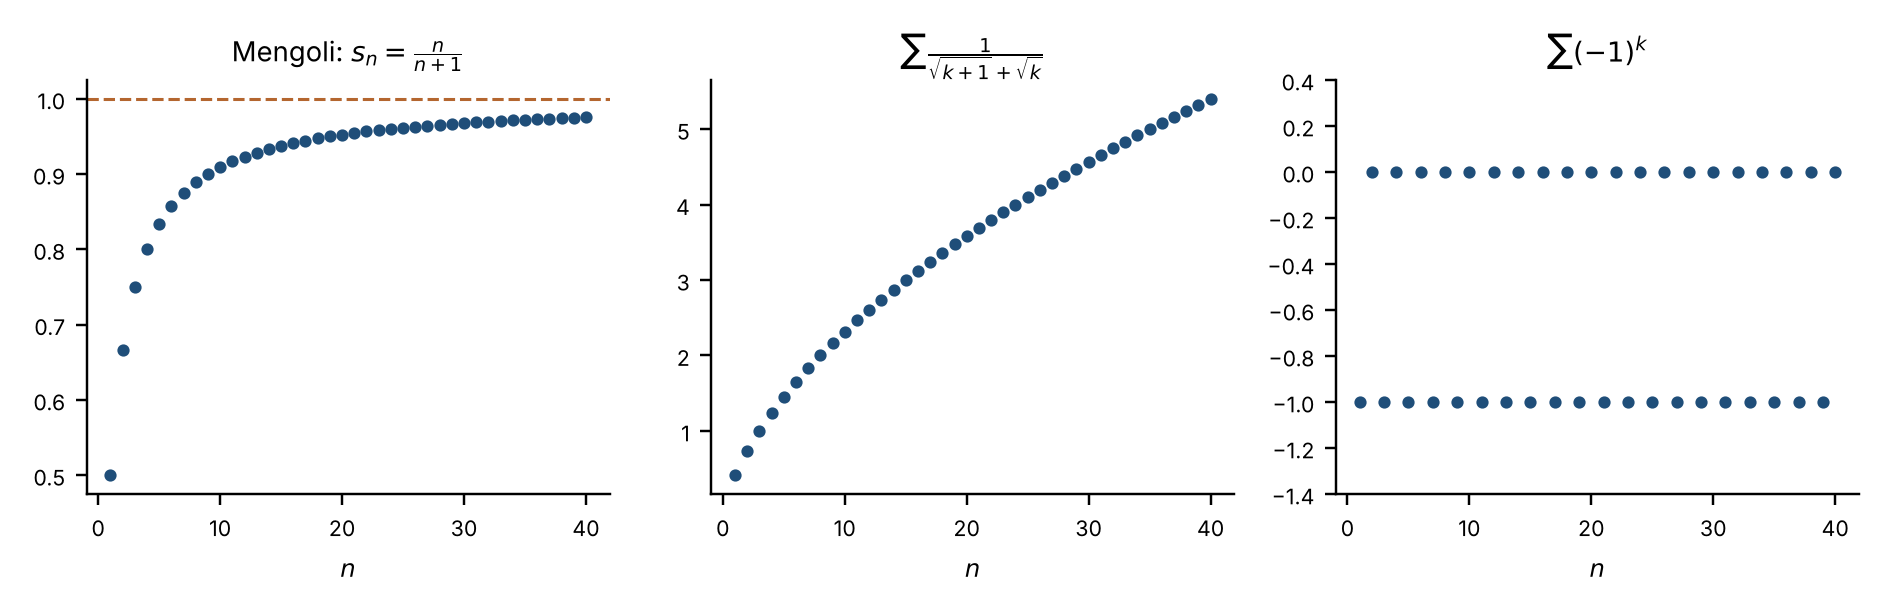
\includegraphics[width=\textwidth]{figure/somme_parziali.png}
\caption{Le somme parziali di tre serie. A sinistra la serie di Mengoli: $s_{n}=\frac n{n+1}$
converge a $1$. Al centro la serie \eqref{eq:serie-radici}: $s_{n}=\sqrt{n+1}-1$ diverge, pur
con termini che tendono a zero. A destra la serie $\sum(-1)^{k}$: le somme parziali
oscillano tra $-1$ e $0$ (\texttt{python/fig\_somme\_parziali.py}).}
\label{fig:somme-parziali}
\end{figure}

\begin{python}[Somme parziali di alcune serie]
import math

def somme_parziali(a, N):
    """Restituisce la lista s_1, ..., s_N delle somme parziali."""
    s, out = 0.0, []
    for k in range(1, N + 1):
        s += a(k)
        out.append(s)
    return out

serie = {
    "Mengoli": lambda k: 1 / (k * (k + 1)),
    "radici":  lambda k: 1 / (math.sqrt(k + 1) + math.sqrt(k)),
    "(-1)^k":  lambda k: (-1)**k,
}
for nome, a in serie.items():
    s = somme_parziali(a, 10000)
    print(f"{nome:8s}: s_10 = {s[9]:9.5f}  s_100 = {s[99]:9.5f}"
          f"  s_10000 = {s[-1]:9.5f}")
\end{python}
\begin{risultato}
Mengoli : s_10 =   0.90909  s_100 =   0.99010  s_10000 =   0.99990
radici  : s_10 =   2.31662  s_100 =   9.04988  s_10000 =  99.00500
(-1)^k  : s_10 =   0.00000  s_100 =   0.00000  s_10000 =   0.00000
\end{risultato}

\needspace{8\baselineskip}
\begin{notastorica}[Da Zenone a Mengoli]
I paradossi di Zenone di Elea (V secolo a.C.), noti attraverso la \emph{Fisica} di
Aristotele, mostrano quanto antica sia la difficoltà di pensare una somma di infiniti
termini. Archimede, nella \emph{Quadratura della parabola}, calcolò di fatto la somma
della serie geometrica $1+\frac14+\frac1{16}+\cdots=\frac43$, evitando però accuratamente
l'infinito con un ragionamento per assurdo (lo abbiamo ripercorso nel
\S\ref{subsec:archimede-parabola}). Non risulta invece che nell'antichità i
paradossi di Zenone siano stati discussi con la serie geometrica: la lettura che ne
daremo nel \S\ref{sec:serie-geometrica} è moderna. Il primo studio sistematico di serie
numeriche si deve al bolognese Pietro Mengoli, allievo di Bonaventura Cavalieri, che nelle
\emph{Novae quadraturae arithmeticae} (1650) sommò la serie che porta il suo nome e altre
serie telescopiche, dimostrò la divergenza della serie armonica e pose il problema di
calcolare $\sum\frac1{k^{2}}$, che sarebbe stato risolto da Eulero quasi un secolo dopo.
\end{notastorica}

%% ----------------------------------------------------------------------------
%%  §11.2  Proprietà delle serie
%% ----------------------------------------------------------------------------
\section{Proprietà delle serie}
\label{sec:proprieta-serie}

Poiché il carattere e la somma di una serie sono definiti mediante il limite delle somme
parziali, le proprietà dei limiti di successioni si traducono in proprietà delle serie.
Cominciamo dalla linearità.

\begin{proposizione}[Linearità]\label{prop:linearita-serie}
\index{serie!linearità}
\begin{enumerate}[label=\textup{(\roman*)}]
  \item Se le serie $\sum a_{k}$ e $\sum b_{k}$ sono regolari e la somma
  $\sum_{k=1}^{\infty}a_{k}+\sum_{k=1}^{\infty}b_{k}$ ha significato in $\overline\R$ (cioè non è della forma
  $+\infty-\infty$), allora la serie $\sum(a_{k}+b_{k})$ è regolare e
  \begin{equation}\label{eq:serie-somma}
    \sum_{k=1}^{\infty}(a_{k}+b_{k})=\sum_{k=1}^{\infty}a_{k}+\sum_{k=1}^{\infty}b_{k} .
  \end{equation}
  \item Se la serie $\sum a_{k}$ è regolare e $c\neq0$ è un numero reale, anche la serie
  $\sum c\,a_{k}$ è regolare e
  \begin{equation}\label{eq:serie-costante}
    \sum_{k=1}^{\infty}c\,a_{k}=c\sum_{k=1}^{\infty}a_{k} ,
  \end{equation}
  con le usuali regole dei segni se la serie diverge. Se $\sum a_{k}$ converge, la
  \eqref{eq:serie-costante} vale anche per $c=0$.
\end{enumerate}
\end{proposizione}

\begin{schema}
\Ipotesi{(i) $\sum a_{k}$, $\sum b_{k}$ regolari, con somme non della forma $+\infty-\infty$; \
(ii) $\sum a_{k}$ regolare, $c\neq0$.}
\Tesi{$\sum(a_{k}+b_{k})=\sum a_{k}+\sum b_{k}$; \ $\sum c\,a_{k}=c\sum a_{k}$.}
\end{schema}

\begin{strategia}
Le somme parziali di $\sum(a_{k}+b_{k})$ e di $\sum c\,a_{k}$ si ottengono da quelle delle serie date
con le operazioni corrispondenti, perché per le somme \emph{finite} le proprietà
associativa, commutativa e distributiva valgono senza restrizioni. Il passaggio al limite
è allora garantito dai teoremi sulle operazioni con i limiti, che escludono proprio le
forme indeterminate $+\infty-\infty$ e $0\cdot\infty$.
\end{strategia}

\begin{dimostrazione}
Le somme parziali di $\sum(a_{k}+b_{k})$ e di $\sum c\,a_{k}$ sono, per le proprietà delle
somme finite, $\sum_{k=1}^{n}(a_{k}+b_{k})=\sum_{k=1}^{n}a_{k}+\sum_{k=1}^{n}b_{k}$ e
$\sum_{k=1}^{n}c\,a_{k}=c\sum_{k=1}^{n}a_{k}$. La tesi segue dai teoremi sulle operazioni con i
limiti, nel caso finito (\cref{teo:operazioni-limiti}) e in quello infinito
(\cref{teo:operazioni-infinite}), esclusi appunto i casi di indeterminazione.
\end{dimostrazione}

Ad esempio, dalla serie di Mengoli si ricava subito
$\sum_{k=1}^{\infty}\frac3{k(k+1)}=3$. Si osservi che la somma di due serie indeterminate può
essere convergente: $\sum(-1)^{k}$ e $\sum(-1)^{k+1}$ sono indeterminate, ma la loro somma è la
serie con tutti i termini nulli.

\subsection{Il resto di una serie}

Le prime somme parziali di una serie possono essere qualsiasi: il carattere dipende
soltanto da ciò che accade «in fondo». Per precisare questa idea, data la serie
$\sum_{k=1}^{\infty}a_{k}$ e fissato $n\in\N$, consideriamo la serie \emph{resto $n$-esimo}
\begin{equation}\label{eq:serie-resto}
  \sum_{k=n+1}^{\infty}a_{k}=a_{n+1}+a_{n+2}+a_{n+3}+\cdots ,
\end{equation}
ottenuta trascurando i primi $n$ termini.

\begin{teorema}[del resto]\label{teo:resto-serie}\index{serie!resto}
Per ogni $n\in\N$ la serie resto $n$-esimo \eqref{eq:serie-resto} ha lo stesso carattere
della serie $\sum_{k=1}^{\infty}a_{k}$. Se la serie converge e $s$ è la sua somma, detta
$R_{n}=\sum_{k=n+1}^{\infty}a_{k}$ la somma del resto, si ha
\begin{equation}\label{eq:resto-serie}
  s=s_{n}+R_{n} \qquad\text{e}\qquad \lim_{n\to+\infty}R_{n}=0 .
\end{equation}
\end{teorema}

\begin{schema}
\Ipotesi{$\sum_{k=1}^{\infty}a_{k}$ serie qualsiasi; \ $n\in\N$ fissato.}
\Tesi{$\sum_{k=n+1}^{\infty}a_{k}$ ha lo stesso carattere di $\sum_{k=1}^{\infty}a_{k}$; \ se
$\sum a_{k}=s\in\R$, allora $R_{n}=s-s_{n}\to0$.}
\end{schema}

\begin{strategia}
Le somme parziali del resto sono differenze di somme parziali della serie data:
$\sum_{k=n+1}^{m}a_{k}=s_{m}-s_{n}$. Con $n$ fissato, $s_{n}$ è una costante, e le due successioni
(nell'indice $m$) hanno lo stesso comportamento. Che il resto tenda a zero è allora la
definizione di convergenza riletta.
\end{strategia}

\begin{dimostrazione}
Fissato $n$, per ogni $m>n$ la somma parziale $(m-n)$-esima del resto è
\[
  \sum_{k=n+1}^{m}a_{k}=\sum_{k=1}^{m}a_{k}-\sum_{k=1}^{n}a_{k}=s_{m}-s_{n} .
\]
Poiché $s_{n}$ non dipende da $m$, la successione $m\mapsto s_{m}-s_{n}$ ha limite (finito o
infinito) se e solo se lo ha $s_{m}$, e i due limiti differiscono per la costante $s_{n}$.
Dunque il resto e la serie hanno lo stesso carattere, e se $s_{m}\to s$ si ha
$R_{n}=\lim_{m\to+\infty}(s_{m}-s_{n})=s-s_{n}$. Infine $R_{n}=s-s_{n}\to s-s=0$ per $n\to+\infty$.
\end{dimostrazione}

Il teorema ha una conseguenza pratica importante: \emph{modificare un numero finito di
termini non cambia il carattere di una serie} (ne cambia, in generale, la somma). Infatti
due serie che differiscono soltanto nei primi $n$ termini hanno lo stesso resto
$n$-esimo. Per questo, nei criteri di convergenza che seguono, le ipotesi potranno essere
richieste soltanto «da un certo indice in poi». Il teorema dice anche che cosa significhi
calcolare la somma di una serie con una somma parziale: l'errore commesso è esattamente
il resto $R_{n}$, e tutto il problema consiste nello \emph{stimarlo}, come abbiamo già fatto
con la formula di Taylor nel \cref{cap:taylor}.

\subsection{Il criterio di Cauchy}

Il criterio di convergenza di Cauchy per le successioni (\cref{teo:criterio-cauchy}),
applicato alle somme parziali, fornisce una condizione necessaria e sufficiente per la
convergenza di una serie che non richiede di conoscerne la somma.

\begin{teorema}[Criterio di Cauchy per le serie]\label{teo:cauchy-serie}
\index{criterio di Cauchy!per le serie}
La serie $\sum_{k=1}^{\infty}a_{k}$ è convergente se e solo se per ogni $\epsilon>0$ esiste
$\nu\in\N$ tale che
\begin{equation}\label{eq:cauchy-serie}
  \Bigl|\sum_{k=n+1}^{n+p}a_{k}\Bigr|=\abs{a_{n+1}+a_{n+2}+\dots+a_{n+p}}<\epsilon
  \qquad\perogni n>\nu,\ \perogni p\in\N .
\end{equation}
\end{teorema}

\begin{schema}
\Ipotesi{$a_{k}$ successione di numeri reali.}
\Tesi{$\sum a_{k}$ convergente $\sse$ $\perogni\epsilon>0\ \esiste\nu$:
$\bigl|\sum_{k=n+1}^{n+p}a_{k}\bigr|<\epsilon$ per ogni $n>\nu$ e ogni $p\in\N$.}
\end{schema}

\begin{strategia}
La serie converge se e solo se la successione $s_{n}$ converge, cioè, per il criterio di
Cauchy, se e solo se $s_{n}$ è di Cauchy. Resta da tradurre la condizione
$\abs{s_{m}-s_{n}}<\epsilon$ in termini degli $a_{k}$: per $m=n+p>n$, la differenza $s_{m}-s_{n}$ è
la somma dei termini da $a_{n+1}$ a $a_{n+p}$.
\end{strategia}

\begin{dimostrazione}
Per il \cref{teo:criterio-cauchy}, la serie converge se e solo se per ogni $\epsilon>0$ esiste
$\nu$ tale che $\abs{s_{m}-s_{n}}<\epsilon$ per ogni $m,n>\nu$. Poiché $\abs{s_{m}-s_{n}}=\abs{s_{n}-s_{m}}$ e
$\abs{s_{n}-s_{n}}=0$, basta considerare le coppie con $m>n$; scritto $m=n+p$ con $p\in\N$,
\[
  s_{m}-s_{n}=\sum_{k=1}^{n+p}a_{k}-\sum_{k=1}^{n}a_{k}=\sum_{k=n+1}^{n+p}a_{k} ,
\]
e la condizione diventa la \eqref{eq:cauchy-serie}.
\end{dimostrazione}

Con $p=1$ la \eqref{eq:cauchy-serie} dà $\abs{a_{n+1}}<\epsilon$ per $n>\nu$: si ritrova la condizione
necessaria del \cref{teo:condizione-necessaria}. Il criterio dice di più: non basta che
i singoli termini siano piccoli, devono essere piccoli anche tutti i «blocchi» di termini
consecutivi, comunque lunghi. Lo useremo per dimostrare il teorema sulla convergenza
assoluta (\S\ref{sec:convergenza-assoluta}) e, nel \S\ref{sec:serie-armonica}, per una terza
dimostrazione della divergenza della serie armonica.

\begin{osservazione}[Parentesi in una serie]\label{oss:parentesi}
Raggruppare con parentesi termini consecutivi di una serie regolare non ne cambia la
somma: le somme parziali della serie raggruppata sono una estratta $s_{n_{1}},s_{n_{2}},\dots$
delle somme parziali della serie data, e un'estratta ha lo stesso limite della
successione (\cref{prop:estratta-limite}). Il viceversa è falso: la serie
$(1-1)+(1-1)+(1-1)+\cdots$ ha tutti i termini nulli e somma $0$, ma togliendo le parentesi si
ottiene la serie indeterminata $1-1+1-1+\cdots$. Le parentesi si possono togliere
liberamente soltanto se si sa già che la serie senza parentesi è regolare.
\end{osservazione}

\begin{osservazione}[Termini nulli]\label{oss:termini-nulli}
Inserire o togliere termini nulli in una serie non ne cambia né il carattere né la
somma. Togliendo gli zeri, infatti, le somme parziali della nuova serie sono un'estratta
di quelle della serie data, e ne hanno lo stesso limite; viceversa, inserendo degli zeri
le somme parziali si ripetono, nello stesso ordine, e le nuove somme parziali hanno lo
stesso limite delle vecchie (se una successione tende a $s$, vi tende anche quella
ottenuta ripetendo un numero finito di volte ciascun termine, come si verifica subito
con la definizione di limite).
\end{osservazione}

%% ----------------------------------------------------------------------------
%%  §11.3  Serie a termini non negativi
%% ----------------------------------------------------------------------------
\section{Serie a termini non negativi}
\label{sec:serie-positive}

Diremo che una serie $\sum a_{k}$ è \emph{a termini non negativi} se $a_{n}\ge0$ per ogni $n$,
e \emph{a termini positivi} se $a_{n}>0$ per ogni $n$. Per queste serie la situazione è
particolarmente semplice, perché la successione delle somme parziali è monotòna: da
$a_{n+1}\ge0$ segue
\begin{equation}\label{eq:somme-crescenti}
  s_{n+1}=s_{n}+a_{n+1}\ge s_{n} \qquad\perogni n\in\N .
\end{equation}

\begin{teorema}[sulle serie a termini non negativi]\label{teo:serie-positive}
\index{serie!a termini non negativi}
Una serie a termini non negativi non può essere indeterminata: è convergente oppure
divergente positivamente. Più precisamente, è convergente se e solo se la successione
delle sue somme parziali è limitata, e in tal caso
\begin{equation}\label{eq:somma-sup}
  \sum_{k=1}^{\infty}a_{k}=\sup_{n\in\N}s_{n} .
\end{equation}
\end{teorema}

\needspace{5\baselineskip}
\begin{schema}
\Ipotesi{$a_{n}\ge0$ per ogni $n$.}
\Tesi{$s_{n}$ ha limite, finito o $+\infty$; \ $\sum a_{k}<+\infty$ $\sse$ $s_{n}$ limitata; \
$\sum a_{k}=\sup s_{n}$.}
\end{schema}

\begin{strategia}
Per la \eqref{eq:somme-crescenti} la successione $s_{n}$ è crescente, e il teorema sulle
successioni monotòne dice tutto: il limite esiste ed è l'estremo superiore, finito se e
solo se la successione è limitata superiormente. Inferiormente $s_{n}$ è limitata da $s_{1}$.
\end{strategia}

\begin{dimostrazione}
Per la \eqref{eq:somme-crescenti} la successione $s_{n}$ è crescente; per il teorema sulle
successioni monotòne (\cref{teo:monotone}) essa ha limite, e $\lim s_{n}=\sup_{n}s_{n}$.
Il limite non può essere $-\infty$, perché $s_{n}\ge s_{1}$ per ogni $n$, e quindi la serie è
convergente o divergente a $+\infty$. Inoltre $\sup_{n}s_{n}<+\infty$ se e solo se $s_{n}$ è
limitata superiormente, cioè (essendo $s_{n}\ge s_{1}$) limitata.
\end{dimostrazione}

In particolare, \emph{la somma di una serie convergente a termini non negativi è
maggiore o uguale a ciascuna delle sue somme parziali}. Per una serie a termini non
negativi si scrive spesso $\sum a_{k}<+\infty$ per dire che la serie converge, e la
condizione necessaria (\cref{teo:condizione-necessaria}) diventa un criterio di
divergenza: se $a_{n}$ non tende a zero, la serie diverge a $+\infty$.

\begin{esempio}\label{es:k-su-k1}
La serie $\sum_{k=1}^{\infty}\frac k{k+1}$ è a termini positivi, quindi convergente o divergente
a $+\infty$. Non è convergente, perché il suo termine generale tende a $1$ e non a $0$.
Dunque $\sum_{k=1}^{\infty}\frac k{k+1}=+\infty$.
\end{esempio}

\begin{esempio}[La serie dei reciproci dei fattoriali]\label{es:serie-fattoriali}
Consideriamo la serie a termini positivi $\sum_{k=0}^{\infty}\frac1{k!}$ (con $0!=1$). Per $k\ge1$
si ha $k!=1\cdot2\cdots k\ge2^{k-1}$, perché ciascuno dei $k-1$ fattori $2,3,\dots,k$ è almeno
$2$. Quindi, per la formula della progressione geometrica (\cref{prop:geometrica}),
\[
  s_{n}=1+\sum_{k=1}^{n}\frac1{k!}\le1+\sum_{k=1}^{n}\frac1{2^{k-1}}=1+\frac{1-2^{-n}}{1-\frac12}<3 :
\]
le somme parziali sono limitate, e la serie converge, con somma compresa tra $s_{1}=2$ e
$3$. La stima del resto \eqref{eq:stima-e} della formula di Taylor dice di più:
$0<e-\sum_{k=0}^{n}\frac1{k!}<\frac3{(n+1)!}\to0$, e quindi
\begin{equation}\label{eq:e-serie}
  \sum_{k=0}^{\infty}\frac1{k!}=1+1+\frac12+\frac1{3!}+\frac1{4!}+\dots=e .
\end{equation}
Il teorema sulle serie a termini non negativi ha garantito l'\emph{esistenza} della
somma con un ragionamento elementare; la formula di Taylor ne ha fornito il
\emph{valore}. (Lo stesso valore si ottiene anche senza Taylor, direttamente dalla
definizione di $e$ come limite di $\bigl(1+\frac1n\bigr)^{n}$: si veda
l'\cref{oss:e-due-vie}.) È il metodo efficiente per il calcolo di $e$ annunciato nel
\cref{cap:successioni}: undici termini danno sette cifre decimali esatte, mentre la
successione $\bigl(1+\frac1n\bigr)^{n}$ ne dà appena cinque con $n=10^{6}$.
\end{esempio}

%% ----------------------------------------------------------------------------
%%  §11.4  La serie geometrica
%% ----------------------------------------------------------------------------
\section{La serie geometrica}
\label{sec:serie-geometrica}

Per ogni numero reale $x$ consideriamo la \emph{serie geometrica} di \emph{ragione} $x$
\begin{equation}\label{eq:serie-geometrica-def}
  \sum_{k=0}^{\infty}x^{k}=1+x+x^{2}+\dots+x^{n}+\cdots .
\end{equation}
È la serie più importante di tutta la teoria: è una delle pochissime di cui si conosce
esplicitamente la somma parziale, e servirà da termine di paragone per molte altre.

\begin{teorema}[Serie geometrica]\label{teo:serie-geometrica}\index{serie!geometrica}
La serie geometrica di ragione $x$ è convergente se $\abs x<1$, divergente
positivamente se $x\ge1$, indeterminata se $x\le-1$. Inoltre
\begin{equation}\label{eq:serie-geometrica}
  \sum_{k=0}^{\infty}x^{k}=\frac1{1-x} \qquad\text{se } -1<x<1 .
\end{equation}
\end{teorema}

\begin{schema}
\Ipotesi{$x\in\R$.}
\Tesi{$\sum x^{k}=\frac1{1-x}$ se $\abs x<1$; \ $\sum x^{k}=+\infty$ se $x\ge1$; \ $\sum x^{k}$
indeterminata se $x\le-1$.}
\end{schema}

\begin{strategia}
Per $x\neq1$ la somma parziale è nota esplicitamente, $s_{n}=\frac{1-x^{n+1}}{1-x}$, e il suo
comportamento dipende soltanto da quello di $x^{n+1}$, che conosciamo dal capitolo sulle
successioni. Il caso $x=1$ si tratta a parte.
\end{strategia}

\begin{dimostrazione}
Se $x=1$, $s_{n}=n+1\to+\infty$. Se $x\neq1$, per la \cref{prop:geometrica}
\begin{equation}\label{eq:somma-parziale-geometrica}
  s_{n}=\sum_{k=0}^{n}x^{k}=\frac{1-x^{n+1}}{1-x} .
\end{equation}
Per il \cref{teo:lim-geometrica}, $x^{n+1}\to0$ se $-1<x<1$, $x^{n+1}\to+\infty$ se $x>1$, e
$x^{n+1}$ non ha limite se $x\le-1$. Nel primo caso $s_{n}\to\frac1{1-x}$. Nel secondo, poiché
$1-x<0$, $s_{n}=\frac{x^{n+1}-1}{x-1}\to+\infty$. Nel terzo, se $s_{n}$ avesse limite $\ell$, anche
$x^{n+1}=1-(1-x)s_{n}$ avrebbe limite $1-(1-x)\ell$ (finito o infinito), il che è falso.
\end{dimostrazione}

Moltiplicando per una costante (\cref{prop:linearita-serie}) e trascurando i primi
termini, si ottiene la forma in cui la serie geometrica si usa più spesso: per $\abs x<1$,
$a\in\R$ e $m\ge0$ intero,
\begin{equation}\label{eq:geometrica-generale}
  \sum_{k=m}^{\infty}a\,x^{k}=a\,x^{m}+a\,x^{m+1}+\dots=\frac{a\,x^{m}}{1-x} ,
\end{equation}
cioè «il primo termine diviso per uno meno la ragione». Ad esempio
$\frac12+\frac14+\frac18+\cdots=\frac{1/2}{1-1/2}=1$, come mostra la \cref{fig:quadrato-geometrico}.

\begin{figure}[htb]
\centering
\begin{tikzpicture}[scale=3.2]
  \fill[blu!35] (0,0) rectangle (0.5,1);
  \fill[blu!25] (0.5,0) rectangle (1,0.5);
  \fill[blu!17] (0.5,0.5) rectangle (0.75,1);
  \fill[blu!11] (0.75,0.5) rectangle (1,0.75);
  \fill[blu!7]  (0.75,0.75) rectangle (0.875,1);
  \fill[blu!4]  (0.875,0.75) rectangle (1,0.875);
  \draw[blu] (0,0) rectangle (1,1);
  \draw[blu] (0.5,0) -- (0.5,1) (0.5,0.5) -- (1,0.5) (0.75,0.5) -- (0.75,1)
    (0.75,0.75) -- (1,0.75) (0.875,0.75) -- (0.875,1) (0.875,0.875) -- (1,0.875);
  \node[font=\small] at (0.25,0.5) {$\frac12$};
  \node[font=\small] at (0.75,0.25) {$\frac14$};
  \node[font=\footnotesize] at (0.625,0.75) {$\frac18$};
  \node[font=\scriptsize] at (0.875,0.625) {$\frac1{16}$};
  \node[font=\tiny] at (0.8125,0.875) {$\frac1{32}$};
\end{tikzpicture}
\caption{La serie geometrica $\frac12+\frac14+\frac18+\cdots=1$: ogni rettangolo è metà della
parte del quadrato unitario non ancora coperta, e i rettangoli riempiono l'intero
quadrato. Le somme parziali sono $1-\frac1{2^{n}}$.}
\label{fig:quadrato-geometrico}
\end{figure}

\subsection{I numeri decimali periodici}

Con la serie geometrica possiamo giustificare la regola, nota dalla scuola media, con
cui un numero decimale periodico si trasforma nella sua \emph{frazione generatrice}. Un
allineamento decimale infinito $0{,}c_{1}c_{2}c_{3}\ldots$, con cifre $c_{k}\in\{0,1,\dots,9\}$, è per
definizione la somma della serie a termini non negativi $\sum_{k=1}^{\infty}c_{k}10^{-k}$, che
converge perché le sue somme parziali sono limitate da $\sum_{k=1}^{\infty}9\cdot10^{-k}=1$.

\begin{proposizione}[Frazione generatrice]\label{prop:periodici}
Sia $0{,}\overline{c_{1}c_{2}\ldots c_{p}}$ un numero decimale periodico semplice con periodo di $p$
cifre, e sia $C=c_{1}c_{2}\ldots c_{p}$ l'intero che ha quelle cifre. Allora
\begin{equation}\label{eq:periodici}
  0{,}\overline{c_{1}c_{2}\ldots c_{p}}=\frac C{10^{p}-1}=\frac C{99\ldots9} ,
\end{equation}
dove il denominatore $99\ldots9$ è formato da $p$ cifre uguali a $9$. In particolare, ogni
numero decimale periodico è razionale.
\end{proposizione}

\begin{schema}
\Ipotesi{$0{,}\overline{c_{1}\ldots c_{p}}=\sum_{k=1}^{\infty}c_{k}10^{-k}$ con $c_{k+p}=c_{k}$; \ $C=c_{1}c_{2}\ldots c_{p}$.}
\Tesi{$0{,}\overline{c_{1}\ldots c_{p}}=\frac C{10^{p}-1}$.}
\end{schema}

\begin{strategia}
Le cifre si ripetono a blocchi di $p$: ogni blocco vale $C$ volte una potenza di
$10^{-p}$, e raggruppando i termini a blocchi la serie delle cifre diventa una serie
geometrica di ragione $10^{-p}$, di cui conosciamo la somma.
\end{strategia}

\begin{dimostrazione}
Il numero è la somma della serie in cui il blocco di cifre si ripete: il primo blocco
vale $C\cdot10^{-p}$, il secondo $C\cdot10^{-2p}$, e così via. Raggruppando le cifre a blocchi
di $p$ (\cref{oss:parentesi}) e usando la \eqref{eq:geometrica-generale} con $x=10^{-p}$,
\[
  0{,}\overline{c_{1}\ldots c_{p}}=\sum_{j=1}^{\infty}C\,10^{-jp}=\frac{C\,10^{-p}}{1-10^{-p}}=\frac C{10^{p}-1} .
\]
Un numero periodico misto si riconduce a questo caso moltiplicando per una potenza di
$10$ e sottraendo l'antiperiodo, che è un numero razionale.
\end{dimostrazione}

Ad esempio $0{,}\overline{13}=\frac{13}{99}$, e $0{,}\overline{9}=\frac99=1$: l'allineamento $0{,}999\ldots$
\emph{non} è «un po' meno» di $1$, ma è esattamente $1$, perché la sua somma è il
\emph{limite} delle somme parziali $1-10^{-n}$. Molte perplessità sull'uguaglianza
$0{,}\overline9=1$ nascono proprio dal confondere una serie con le sue somme parziali.

\subsection{Il paradosso di Achille}

\begin{idea}[Achille e la tartaruga, in volo]
Un velivolo $A$ insegue alla velocità $v_{A}$ un velivolo $B$ che lo precede di una
distanza $d$ e vola sulla stessa rotta alla velocità $v_{B}<v_{A}$. Ragioniamo come
Zenone (\cref{fig:zenone}). Nel tempo $t_{0}=\frac d{v_{A}}$ che $A$ impiega a raggiungere la
posizione iniziale di $B$, questo avanza di $d\,\frac{v_{B}}{v_{A}}$; nel tempo $t_{1}=t_{0}\frac{v_{B}}{v_{A}}$ che
$A$ impiega a colmare questo nuovo distacco, $B$ avanza di $d\bigl(\frac{v_{B}}{v_{A}}\bigr)^{2}$; e così
via. I tempi $t_{k}=t_{0}q^{k}$, con $q=\frac{v_{B}}{v_{A}}<1$, sono infiniti, ma la loro somma è la
serie geometrica
\[
  T=\sum_{k=0}^{\infty}\frac d{v_{A}}\,q^{k}=\frac d{v_{A}}\cdot\frac1{1-\frac{v_{B}}{v_{A}}}=\frac d{v_{A}-v_{B}} ,
\]
che è finita, ed è proprio il tempo che si ottiene ragionando con la velocità relativa
$v_{A}-v_{B}$. Ad esempio, con $d=20$~km, $v_{A}=900$~km/h e $v_{B}=750$~km/h, il
raggiungimento avviene dopo $T=\frac{20}{150}$~h, cioè $8$~minuti. Dal punto di vista matematico, il
paradosso nasce dal supporre che infiniti intervalli di tempo debbano avere una durata
complessiva infinita. (Aristotele, che riferisce l'argomento, rispondeva distinguendo
l'infinito «in atto» da quello «in potenza»: un dibattito filosofico che la definizione
di somma di una serie non esaurisce, ma rende innocuo per il calcolo.)
\end{idea}

\begin{figure}[htb]
\centering
\begin{tikzpicture}[x=0.95cm]
  \draw[grigio, -{Stealth[length=2mm]}] (-0.3,0) -- (10.6,0) node[above, font=\scriptsize] {rotta};
  \foreach \x/\lab in {0/{$A_{0}$}, 4/{$A_{1}=B_{0}$}, 6.4/{$A_{2}=B_{1}$}, 7.84/{$B_{2}$}}
    \fill (\x,0) circle (1.4pt) node[below=2pt, font=\scriptsize] {\lab};
  \fill (8.704,0) circle (1pt);
  \fill (9.222,0) circle (1pt);
  \fill (9.533,0) circle (0.8pt);
  \draw[rame, thick] (10,-0.12) -- (10,0.12);
  \node[rame, font=\scriptsize, below=2pt] at (10,0) {incontro};
  \draw[blu, -{Stealth[length=1.6mm]}] (0,0.35) -- node[above, font=\scriptsize] {$t_{0}$} (4,0.35);
  \draw[blu, -{Stealth[length=1.6mm]}] (4,0.35) -- node[above, font=\scriptsize] {$t_{1}=qt_{0}$} (6.4,0.35);
  \draw[blu, -{Stealth[length=1.6mm]}] (6.4,0.35) -- node[above, font=\scriptsize] {$t_{2}$} (7.84,0.35);
  \draw[blu, -{Stealth[length=1.6mm]}] (7.84,0.35) -- (8.704,0.35);
\end{tikzpicture}
\caption{Il ragionamento di Zenone per l'inseguimento ($q=\frac{v_{B}}{v_{A}}=0{,}6$ nel disegno):
$A$ raggiunge successivamente le posizioni $B_{0},B_{1},B_{2},\dots$ occupate da $B$ un passo
prima. I tratti, e i tempi, formano una progressione geometrica di ragione $q$, e la loro
somma è finita: l'incontro avviene a distanza $\frac d{1-q}$ dal punto di partenza di $A$.}
\label{fig:zenone}
\end{figure}

\begin{python}[Serie geometrica e frazioni generatrici]
from fractions import Fraction as F

def periodico(antiperiodo, periodo):
    """Frazione di 0,antiperiodo(periodo), es. ('1', '6') -> 1/6."""
    m, p = len(antiperiodo), len(periodo)
    A = int(antiperiodo) if antiperiodo else 0
    C = int(periodo)
    # 0,a(c) = (A + C/(10^p - 1)) / 10^m
    return (A + F(C, 10**p - 1)) / 10**m

for a, c in (("", "13"), ("", "9"), ("1", "6"), ("", "142857")):
    print(f"0,{a}({c}) = {periodico(a, c)}")

x = 0.6                                    # somme parziali, q = 0,6
s = [sum(x**k for k in range(n + 1)) for n in (5, 10, 20, 40)]
print("s_n:", [round(v, 8) for v in s], " 1/(1-x) =", 1 / (1 - x))
\end{python}
\begin{risultato}
0,(13) = 13/99
0,(9) = 1
0,1(6) = 1/6
0,(142857) = 1/7
s_n: [2.38336, 2.49093007, 2.49994516, 2.5]  1/(1-x) = 2.5
\end{risultato}

\begin{notastorica}[Eulero e le «somme» delle serie divergenti]
La formula \eqref{eq:serie-geometrica} vale soltanto per $-1<x<1$, ma per tutto il
Settecento fu usata spesso senza questa restrizione. Con $x=-1$ se ne ricava
$1-1+1-1+\cdots=\frac12$: il camaldolese Guido Grandi, professore a Pisa, vi vide nel 1703
un'immagine della creazione dal nulla, e Leibniz, in una lettera a Christian Wolff
pubblicata nel 1713, difese il valore $\frac12$ osservando che le somme parziali valgono $1$
e $0$ «con uguale probabilità». Con $x=2$ si ottiene addirittura $-1=1+2+4+8+\cdots$.
Eulero discusse proprio questa uguaglianza nella memoria \emph{De seriebus divergentibus}
(1760), e propose di chiamare somma di una serie l'espressione finita dal cui sviluppo
essa nasce, qui $\frac1{1-x}$: nelle sue mani la regola condusse a scoperte profonde, in mani
meno esperte a contraddizioni. Cauchy, nel \emph{Cours d'analyse} (1821), tagliò il nodo
con la definizione che abbiamo adottato: una serie divergente non ha somma, e le
operazioni sulle serie sono lecite soltanto per quelle convergenti. Nel 1826 il giovane
Niels Henrik Abel scriveva a un amico che le serie divergenti sono «qualcosa di funesto»,
su cui è una vergogna fondare una dimostrazione. Più tardi si capì come recuperare in
modo coerente almeno una parte di quei valori: Ernesto Cesàro (1890) propose di
sostituire alle somme parziali le loro medie aritmetiche, che per la serie di Grandi
tendono proprio a $\frac12$. Nacque così la teoria della \emph{sommabilità}, che non
contraddice la definizione di Cauchy, ma la estende.
\end{notastorica}

%% ----------------------------------------------------------------------------
%%  §11.5  La serie armonica
%% ----------------------------------------------------------------------------
\section{La serie armonica}
\label{sec:serie-armonica}

La serie
\begin{equation}\label{eq:serie-armonica}
  \sum_{k=1}^{\infty}\frac1k=1+\frac12+\frac13+\dots+\frac1n+\cdots
\end{equation}
si chiama \emph{serie armonica}\index{serie!armonica}. Il suo termine generale tende a zero,
e le somme parziali crescono molto lentamente: ci vogliono più di dodicimila termini
perché superino $10$. Eppure la serie diverge. Poiché il risultato è importante e un po'
sorprendente, ne diamo tre dimostrazioni, ciascuna delle quali insegna qualcosa.

\begin{teorema}[Divergenza della serie armonica]\label{teo:armonica}
La serie armonica è divergente: $\sum_{k=1}^{\infty}\frac1k=+\infty$. Più precisamente, le sue
somme parziali $H_{n}=\sum_{k=1}^{n}\frac1k$ verificano
\begin{equation}\label{eq:armonica-log}
  H_{n}\ge\log(n+1) \qquad\perogni n\in\N .
\end{equation}
\end{teorema}

\begin{schema}
\Ipotesi{$H_{n}=\sum_{k=1}^{n}\frac1k$.}
\Tesi{$H_{n}\ge\log(n+1)$ per ogni $n$; \ quindi $H_{n}\to+\infty$.}
\end{schema}

\begin{strategia}
Confrontiamo la somma con un'area. Il termine $\frac1k$ è l'area di un rettangolo di base
$[k,k+1]$ e altezza $\frac1k$, che contiene la regione sotto il grafico di $\frac1x$ nello stesso
intervallo, perché $\frac1x\le\frac1k$ per $x\ge k$ (\cref{fig:armonica-integrale}, a sinistra).
Sommando, $H_{n}$ supera l'integrale di $\frac1x$ tra $1$ e $n+1$, cioè $\log(n+1)$, che diverge.
\end{strategia}

\begin{dimostrazione}[Prima dimostrazione (con l'integrale)]
Per ogni $k\in\N$ e ogni $x\in[k,k+1]$ si ha $\frac1x\le\frac1k$. Per il confronto tra integrali
(\cref{teo:confronto-integrali}),
\begin{equation}\label{eq:armonica-rettangolo}
  \int_{k}^{k+1}\frac{dx}x\le\int_{k}^{k+1}\frac{dx}k=\frac1k .
\end{equation}
Sommando per $k$ da $1$ a $n$ e usando l'additività dell'integrale (\cref{teo:additivita})
e la formula fondamentale del calcolo integrale,
\[
  H_{n}=\sum_{k=1}^{n}\frac1k\ge\sum_{k=1}^{n}\int_{k}^{k+1}\frac{dx}x=\int_{1}^{n+1}\frac{dx}x=\log(n+1) .
\]
Poiché $\log(n+1)\to+\infty$, per il teorema del confronto (\cref{teo:confronto-infinito})
anche $H_{n}\to+\infty$.
\end{dimostrazione}

La seconda dimostrazione ottiene la stessa disuguaglianza senza il calcolo integrale,
usando le proprietà del numero $e$.

\begin{dimostrazione}[Seconda dimostrazione (con il numero $e$)]
Per il \cref{teo:numero-e} si ha $\bigl(1+\frac1k\bigr)^{k}<e$ per ogni $k\in\N$. Poiché il
logaritmo è crescente,
\[
  k\log\Bigl(1+\frac1k\Bigr)=\log\Bigl(1+\frac1k\Bigr)^{k}<\log e=1 ,
\]
cioè
\[
  \frac1k>\log\frac{k+1}k=\log(k+1)-\log k .
\]
Sommando per $k=1,\dots,n$, il secondo membro è una somma telescopica
(\cref{prop:serie-telescopica}):
$H_{n}>\log(n+1)-\log1=\log(n+1)$.
\end{dimostrazione}

La terza dimostrazione, la più antica, raggruppa i termini a blocchi e usa il criterio di
Cauchy.

\begin{dimostrazione}[Terza dimostrazione (con il criterio di Cauchy)]
Per ogni $n\in\N$, il blocco dei $n$ termini da $\frac1{n+1}$ a $\frac1{2n}$ verifica
\[
  \sum_{k=n+1}^{2n}\frac1k=\frac1{n+1}+\frac1{n+2}+\dots+\frac1{2n}\ge n\cdot\frac1{2n}=\frac12 ,
\]
perché ciascuno dei suoi $n$ termini è almeno $\frac1{2n}$. Dunque la condizione
\eqref{eq:cauchy-serie} è violata con $\epsilon=\frac12$ e $p=n$, per ogni $n$: la serie non
converge (\cref{teo:cauchy-serie}). Essendo a termini positivi, diverge a $+\infty$
(\cref{teo:serie-positive}).
\end{dimostrazione}

\begin{figure}[htb]
\centering
\begin{tikzpicture}
\begin{axis}[width=0.53\textwidth, height=4.6cm, xmin=0, xmax=8.6, ymin=0, ymax=1.15,
  axis lines=left, xtick={1,2,...,8}, ytick={0,0.5,1}, axis on top,
  title={\scriptsize $H_{n}\ge\int_{1}^{n+1}\frac{dx}x$}, tick label style={font=\scriptsize}]
  \addplot[fill=blu!20, draw=blu, ybar interval]
    coordinates {(1,1) (2,0.5) (3,0.3333) (4,0.25) (5,0.2) (6,0.1667) (7,0.1429) (8,0)};
  \addplot[curva, domain=0.87:8.6, samples=80] {1/x};
\end{axis}
\end{tikzpicture}\hfill
\begin{tikzpicture}
\begin{axis}[width=0.53\textwidth, height=4.6cm, xmin=0, xmax=8.6, ymin=0, ymax=1.15,
  axis lines=left, xtick={1,2,...,8}, ytick={0,0.5,1}, axis on top,
  title={\scriptsize $H_{n+1}-1\le\int_{1}^{n+1}\frac{dx}x$}, tick label style={font=\scriptsize}]
  \addplot[fill=rame!30, draw=rame, ybar interval]
    coordinates {(1,0.5) (2,0.3333) (3,0.25) (4,0.2) (5,0.1667) (6,0.1429) (7,0.125) (8,0)};
  \addplot[curva, domain=0.87:8.6, samples=80] {1/x};
\end{axis}
\end{tikzpicture}
\caption{Il confronto tra la serie armonica e l'integrale di $\frac1x$. A sinistra i
rettangoli di altezza $\frac1k$ sulle basi $[k,k+1]$ contengono la regione sotto il grafico:
$H_{n}\ge\log(n+1)$. A destra i rettangoli di altezza $\frac1{k+1}$ sono contenuti in essa:
$H_{n+1}-1\le\log(n+1)$. Le somme parziali sono quindi «intrappolate» tra due logaritmi.}
\label{fig:armonica-integrale}
\end{figure}

\subsection{Il criterio dell'integrale e la serie armonica generalizzata}

Il ragionamento della prima dimostrazione funziona per ogni funzione positiva e
decrescente, e collega il carattere di una serie a quello di un integrale improprio
(\S\ref{sec:impropri}).

\begin{teorema}[Criterio dell'integrale]\label{teo:criterio-integrale}
\index{criterio dell'integrale}
Sia $f$ continua, non negativa e decrescente in $[1,+\infty)$, e sia $a_{k}=f(k)$. Allora
per ogni $n\in\N$
\begin{equation}\label{eq:criterio-integrale}
  \int_{1}^{n+1}f(x)\,dx\le\sum_{k=1}^{n}a_{k}\le a_{1}+\int_{1}^{n}f(x)\,dx ,
\end{equation}
e la serie $\sum_{k=1}^{\infty}a_{k}$ converge se e solo se converge l'integrale improprio
$\int_{1}^{+\infty}f(x)\,dx$. In tal caso il resto $R_{n}=\sum_{k=n+1}^{\infty}a_{k}$ verifica
\begin{equation}\label{eq:resto-integrale-serie}
  \int_{n+1}^{+\infty}f(x)\,dx\le R_{n}\le\int_{n}^{+\infty}f(x)\,dx .
\end{equation}
\end{teorema}

\begin{schema}
\Ipotesi{$f$ continua, $f\ge0$, decrescente in $[1,+\infty)$; \ $a_{k}=f(k)$.}
\Tesi{la \eqref{eq:criterio-integrale}; \ $\sum a_{k}<+\infty$ $\sse$
$\int_{1}^{+\infty}f<+\infty$; \ la stima \eqref{eq:resto-integrale-serie} del resto.}
\end{schema}

\begin{strategia}
Come nella \cref{fig:armonica-integrale}: nell'intervallo $[k,k+1]$ la funzione
decrescente sta tra $f(k+1)$ e $f(k)$, e integrando si ottiene
$a_{k+1}\le\int_{k}^{k+1}f\le a_{k}$. Sommando si ottengono le due stime. Le somme parziali e la
funzione integrale $b\mapsto\int_{1}^{b}f$ sono entrambe crescenti, e le stime dicono che una è
limitata se e solo se lo è l'altra.
\end{strategia}

\begin{dimostrazione}
Per $x\in[k,k+1]$ la monotonia dà $f(k+1)\le f(x)\le f(k)$, e per il confronto tra
integrali
\begin{equation}\label{eq:integrale-intrappolato}
  a_{k+1}\le\int_{k}^{k+1}f(x)\,dx\le a_{k} \qquad\perogni k\in\N .
\end{equation}
Sommando la disuguaglianza di destra per $k=1,\dots,n$ si ottiene
$\int_{1}^{n+1}f\le\sum_{k=1}^{n}a_{k}$; sommando quella di sinistra per $k=1,\dots,n-1$ si ottiene
$\sum_{k=2}^{n}a_{k}\le\int_{1}^{n}f$, cioè la seconda delle \eqref{eq:criterio-integrale}.

Poiché $f\ge0$, la funzione $F(b)=\int_{1}^{b}f$ è crescente, e per il \cref{lem:monotona-infinito}
ha limite per $b\to+\infty$, finito se e solo se $F$ è limitata; inoltre, essendo crescente,
$F$ è limitata se e solo se lo è la successione $F(n)$. Le \eqref{eq:criterio-integrale}
mostrano che $s_{n}$ è limitata se e solo se $F(n)$ lo è, e per il \cref{teo:serie-positive}
la serie converge se e solo se converge l'integrale.

Infine, sommando le \eqref{eq:integrale-intrappolato} per $k$ da $n+1$ a $m$ si ha
$\int_{n+1}^{m+1}f\le\sum_{k=n+1}^{m}a_{k}$ e, per $k$ da $n$ a $m-1$, $\sum_{k=n+1}^{m}a_{k}\le\int_{n}^{m}f$;
per $m\to+\infty$ si ottiene la \eqref{eq:resto-integrale-serie}.
\end{dimostrazione}

\begin{teorema}[Serie armonica generalizzata]\label{teo:armonica-generalizzata}
\index{serie!armonica generalizzata}
La serie
\begin{equation}\label{eq:armonica-generalizzata}
  \sum_{k=1}^{\infty}\frac1{k^{p}}=1+\frac1{2^{p}}+\frac1{3^{p}}+\dots+\frac1{n^{p}}+\cdots
\end{equation}
è convergente se $p>1$ ed è divergente se $p\le1$.
\end{teorema}

\begin{schema}
\Ipotesi{$p\in\R$.}
\Tesi{$\sum\frac1{k^{p}}<+\infty$ $\sse$ $p>1$.}
\end{schema}

\begin{strategia}
Per $p>0$ la funzione $\frac1{x^{p}}$ è positiva e decrescente, e il criterio dell'integrale
riduce il problema all'integrale improprio $\int_{1}^{+\infty}\frac{dx}{x^{p}}$, già calcolato nel
\cref{cap:integrali-indefiniti}. Per $p\le0$ il termine generale non tende a zero.
\end{strategia}

\begin{dimostrazione}
Se $p\le0$, $\frac1{k^{p}}=k^{-p}\ge1$ non tende a zero, e la serie (a termini positivi) diverge
per il \cref{teo:condizione-necessaria}. Se $p>0$, la funzione $f(x)=x^{-p}$ è continua,
positiva e decrescente in $[1,+\infty)$; per il \cref{teo:criterio-integrale} e la
\eqref{eq:impropri-p-infinito}, la serie converge se e solo se $p>1$.
\end{dimostrazione}

Per $p>1$ la \eqref{eq:criterio-integrale} dà anche
$\frac{(n+1)^{1-p}-1}{1-p}\le s_{n}\le1+\frac{1-n^{1-p}}{p-1}$, e passando al limite
$\frac1{p-1}\le\sum_{k=1}^{\infty}\frac1{k^{p}}\le\frac p{p-1}$. Ad esempio $1\le\sum\frac1{k^{2}}\le2$; il valore esatto
è $\frac{\pi^{2}}6\approx1{,}6449$, come scoprì Eulero nel 1734. La stima del resto
\eqref{eq:resto-integrale-serie} con $f(x)=\frac1{x^{2}}$ dice che
$\frac1{n+1}\le\frac{\pi^{2}}6-\sum_{k=1}^{n}\frac1{k^{2}}\le\frac1n$: con cento termini si ottiene una sola cifra
decimale esatta (l'errore è circa $10^{-2}$).

\subsection{La costante di Eulero--Mascheroni}

Le somme parziali della serie armonica divergono, ma in modo molto regolare: sono vicine
a $\log n$, e la differenza ha un limite.

\begin{proposizione}[Costante di Eulero--Mascheroni]\label{prop:eulero-mascheroni}
\index{costante di Eulero--Mascheroni}
La successione $d_{n}=H_{n}-\log n$ è decrescente e verifica $0\le d_{n}\le1$. Il suo limite
\begin{equation}\label{eq:eulero-mascheroni}
  \gamma=\lim_{n\to+\infty}\Bigl(1+\frac12+\dots+\frac1n-\log n\Bigr)=0{,}5772156649\ldots
\end{equation}
si chiama \emph{costante di Eulero--Mascheroni}. In particolare $H_{n}=\log n+\gamma+o(1)$.
\end{proposizione}

\begin{schema}
\Ipotesi{$d_{n}=H_{n}-\log n$.}
\Tesi{$d_{n+1}\le d_{n}$; \ $0\le d_{n}\le1$; \ quindi $d_{n}\to\gamma\in[0,1]$.}
\end{schema}

\begin{strategia}
Basta mostrare che $d_{n}$ è monotòna e limitata. La differenza $d_{n}-d_{n+1}$ è l'area compresa,
nell'intervallo $[n,n+1]$, tra il grafico di $\frac1x$ e il rettangolo di altezza $\frac1{n+1}$:
è positiva. La limitazione dal basso viene dalla stima \eqref{eq:armonica-log}, che dice
che $H_{n}$ supera $\log(n+1)$, e quindi anche $\log n$.
\end{strategia}

\begin{dimostrazione}
Si ha $d_{n}-d_{n+1}=\log(n+1)-\log n-\frac1{n+1}=\int_{n}^{n+1}\bigl(\frac1x-\frac1{n+1}\bigr)dx\ge0$,
perché l'integrando è non negativo in $[n,n+1]$: la successione è decrescente, e quindi
$d_{n}\le d_{1}=1$. Inoltre, per la \eqref{eq:armonica-log},
$d_{n}\ge\log(n+1)-\log n>0$. Per il teorema sulle successioni monotòne $d_{n}$ converge a un
limite $\gamma\in[0,1]$.
\end{dimostrazione}

La relazione $H_{n}\approx\log n+\gamma$ spiega la lentezza della divergenza: per avere
$H_{n}>10$ occorre $n\approx e^{10-\gamma}\approx12\,367$, e per $H_{n}>100$ un numero di termini
dell'ordine di $10^{43}$. Non si sa ancora se $\gamma$ sia un numero razionale.

\begin{python}[Serie armonica, costante di Eulero e problema di Basilea]
import math

H, n = 0.0, 0
while H <= 10:                        # primo n con H_n > 10
    n += 1
    H += 1 / n
print(f"H_n > 10 per la prima volta con n = {n}")

H, N = 0.0, 1
for k in range(1, 10**6 + 1):
    H += 1 / k
    if k == N:
        print(f"n = {k:>7}:  H_n - log n = {H - math.log(k):.8f}")
        N *= 10

s = sum(1 / k**2 for k in range(1, 101))
print(f"pi^2/6 - s_100 = {math.pi**2 / 6 - s:.6f}"
      f"   (stima: tra {1/101:.6f} e {1/100:.6f})")
\end{python}
\begin{risultato}
H_n > 10 per la prima volta con n = 12367
n =       1:  H_n - log n = 1.00000000
n =      10:  H_n - log n = 0.62638316
n =     100:  H_n - log n = 0.58220733
n =    1000:  H_n - log n = 0.57771558
n =   10000:  H_n - log n = 0.57726566
n =  100000:  H_n - log n = 0.57722066
n = 1000000:  H_n - log n = 0.57721616
pi^2/6 - s_100 = 0.009950   (stima: tra 0.009901 e 0.010000)
\end{risultato}

\subsection{Approfondimento: il criterio di condensazione di Cauchy}
\label{subsec:condensazione}

La terza dimostrazione della divergenza della serie armonica raggruppava i termini in
blocchi sempre più lunghi. Se i blocchi hanno lunghezza $1,2,4,8,\dots$, l'idea funziona
per ogni successione non negativa e decrescente, e conduce a un criterio, dovuto a
Cauchy (\emph{Cours d'analyse}, 1821), che non richiede il calcolo integrale: la serie
data ha lo stesso carattere di una serie formata soltanto dai termini di indice $2^{k}$,
ciascuno moltiplicato per $2^{k}$, cioè per il numero dei termini del blocco che
rappresenta.

\begin{teorema}[Criterio di condensazione]\label{teo:condensazione}
\index{criterio di condensazione}
Sia $a_{n}$ una successione non negativa e decrescente. Allora le serie
\begin{equation}\label{eq:condensazione}
  \sum_{n=1}^{\infty}a_{n} \qquad\text{e}\qquad
  \sum_{k=0}^{\infty}2^{k}a_{2^{k}}=a_{1}+2a_{2}+4a_{4}+8a_{8}+\cdots
\end{equation}
hanno lo stesso carattere. Più precisamente, dette $s_{n}=\sum_{j=1}^{n}a_{j}$ e
$t_{m}=\sum_{k=0}^{m}2^{k}a_{2^{k}}$ le somme parziali delle due serie, per ogni intero $m\ge0$
\begin{equation}\label{eq:condensazione-stime}
  \tfrac12\,t_{m}\le s_{2^{m}} \qquad\text{e}\qquad s_{2^{m+1}-1}\le t_{m} .
\end{equation}
\end{teorema}

\begin{schema}
\Ipotesi{$a_{n}\ge0$; \ $a_{n+1}\le a_{n}$ per ogni $n\in\N$.}
\Tesi{$\sum a_{n}<+\infty$ $\sse$ $\sum 2^{k}a_{2^{k}}<+\infty$; \ le stime
\eqref{eq:condensazione-stime}.}
\end{schema}

\begin{strategia}
Si dividono gli indici in blocchi compresi tra due potenze di $2$ consecutive. Il blocco
da $2^{k}$ a $2^{k+1}-1$ ha $2^{k}$ termini, tutti non maggiori del primo, $a_{2^{k}}$, perché la
successione decresce; il blocco da $2^{k-1}+1$ a $2^{k}$ ha $2^{k-1}$ termini, tutti non minori
dell'ultimo, $a_{2^{k}}$. Sommando sui blocchi si ottengono le due stime, e per le serie a
termini non negativi la limitatezza delle somme parziali passa dall'una all'altra.
\end{strategia}

\begin{dimostrazione}
Per ogni $k\ge0$ il blocco degli indici $j$ con $2^{k}\le j\le2^{k+1}-1$ contiene $2^{k}$ indici,
e per la monotonia $a_{j}\le a_{2^{k}}$; quindi la somma dei termini del blocco è al più
$2^{k}a_{2^{k}}$. Gli indici da $1$ a $2^{m+1}-1$ sono l'unione dei blocchi con $k=0,1,\dots,m$, e
sommando si ottiene $s_{2^{m+1}-1}\le\sum_{k=0}^{m}2^{k}a_{2^{k}}=t_{m}$.

Per ogni $k\ge1$ il blocco degli indici $j$ con $2^{k-1}+1\le j\le2^{k}$ contiene $2^{k-1}$ indici, e
$a_{j}\ge a_{2^{k}}$; la somma dei suoi termini è quindi almeno $2^{k-1}a_{2^{k}}$. Gli indici da $2$
a $2^{m}$ sono l'unione di questi blocchi con $k=1,\dots,m$, e
\[
  s_{2^{m}}\ge a_{1}+\sum_{k=1}^{m}2^{k-1}a_{2^{k}}=a_{1}+\tfrac12\,(t_{m}-a_{1})\ge\tfrac12\,t_{m} .
\]
Le due serie sono a termini non negativi, e per il \cref{teo:serie-positive} basta
confrontare la limitatezza delle somme parziali. Se $t_{m}\le T$ per ogni $m$, dato $n$ si
ha $n\le2^{n+1}-1$, e poiché $s_{n}$ è crescente $s_{n}\le s_{2^{n+1}-1}\le t_{n}\le T$: le $s_{n}$ sono limitate.
Se invece $s_{n}\le S$ per ogni $n$, la prima stima dà $t_{m}\le2s_{2^{m}}\le2S$. Dunque le due
serie convergono o divergono insieme.
\end{dimostrazione}

Passando al limite nelle \eqref{eq:condensazione-stime}, la somma della serie data risulta
compresa tra la metà della somma della serie condensata e la somma stessa. Il criterio
richiede soltanto la monotonia, non una funzione continua di cui calcolare l'integrale:
è la versione «discreta» del criterio dell'integrale.

\begin{esempio}[L'armonica generalizzata senza integrali]\label{es:condensazione-armonica}
Ritroviamo il \cref{teo:armonica-generalizzata}. Se $p\le0$, il termine generale non
tende a zero. Se $p>0$, la successione $a_{n}=n^{-p}$ è positiva e decrescente, e
\[
  2^{k}a_{2^{k}}=2^{k}\,(2^{k})^{-p}=\bigl(2^{1-p}\bigr)^{k} :
\]
la serie condensata è la serie geometrica di ragione $2^{1-p}>0$, che converge se e solo
se $2^{1-p}<1$, cioè $p>1$ (\cref{teo:serie-geometrica}). Per $p=1$ la serie condensata
è $1+1+1+\cdots$: è l'argomento di Oresme. Per $p>1$ si ha anche
$\sum_{n\ge1}\frac1{n^{p}}\le\frac1{1-2^{1-p}}$, che per $p=2$ vale $2$.
\end{esempio}

\begin{esempio}[Serie con il logaritmo]\label{es:condensazione-log}
Sia $p>0$. I termini della serie $\sum_{n=2}^{\infty}\frac1{n(\log n)^{p}}$ sono positivi e
decrescenti, perché il denominatore cresce; ponendo $a_{1}=a_{2}$, il che non cambia il carattere (\cref{teo:resto-serie}),
si può applicare il criterio. Per $k\ge1$
\[
  2^{k}a_{2^{k}}=\frac{2^{k}}{2^{k}\,(k\log2)^{p}}=\frac1{(\log2)^{p}}\cdot\frac1{k^{p}} ,
\]
e la serie condensata è, a meno della costante $(\log2)^{-p}$, la serie armonica
generalizzata di esponente $p$. Dunque $\sum_{n\ge2}\frac1{n(\log n)^{p}}$ converge se e solo se
$p>1$. Per $p=1$ si ottiene la divergenza di $\sum\frac1{n\log n}$, una serie che, come
vedremo nel \S\ref{sec:criteri-convergenza}, sfugge al criterio degli infinitesimi.
\end{esempio}

\begin{notastorica}[Oresme, i Bernoulli, Eulero]
La terza dimostrazione della divergenza della serie armonica risale a Nicola d'Oresme,
che intorno al 1350 raggruppò i termini a blocchi di lunghezza $1,2,4,8,\dots$, ciascuno di
somma almeno $\frac12$: sono i blocchi da $\frac1{n+1}$ a $\frac1{2n}$ con $n=2^{j}$: è il criterio di
condensazione applicato alla serie armonica. La dimostrazione cadde nell'oblio e il risultato fu ritrovato da Pietro
Mengoli (1650) e dai fratelli Jakob e Johann Bernoulli (1689). Il problema di calcolare
$\sum\frac1{k^{2}}$, posto da Mengoli, divenne noto come \emph{problema di Basilea}, dalla città
dei Bernoulli, che non riuscirono a risolverlo; lo risolse nel 1734 il giovane Eulero,
che trovò $\frac{\pi^{2}}6$ con un ragionamento audace, reso rigoroso solo in seguito. Nello
stesso periodo Eulero introdusse la costante $\gamma$; Lorenzo Mascheroni, matematico di
Bergamo, ne calcolò nel 1790 trentadue cifre decimali, non tutte esatte.
\end{notastorica}

%% ----------------------------------------------------------------------------
%%  §11.6  Criteri di convergenza per le serie a termini non negativi
%% ----------------------------------------------------------------------------
\section{Criteri di convergenza}
\label{sec:criteri-convergenza}

Calcolare esplicitamente la somma di una serie è possibile solo in pochi casi (le
serie geometriche, le telescopiche, poche altre); per questo, nelle applicazioni, la somma
si calcola spesso numericamente. Prima di farlo, però, occorre sapere se la serie
converge: sommare con un calcolatore il primo milione di termini della serie armonica
darebbe circa $14{,}4$, un numero del tutto privo di significato come «somma». I \emph{criteri di
convergenza} stabiliscono il carattere di una serie senza calcolarne la somma. In tutto
questo paragrafo consideriamo serie \emph{a termini non negativi}, che per il
\cref{teo:serie-positive} sono convergenti o divergenti a $+\infty$. Per il teorema del resto
(\cref{teo:resto-serie}) basta che le ipotesi siano verificate da un certo indice in poi.

\subsection{Il criterio del confronto}

\begin{teorema}[Criterio del confronto]\label{teo:confronto-serie}
\index{criterio del confronto!per le serie}
Siano $a_{n}$ e $b_{n}$ due successioni tali che $0\le a_{n}\le b_{n}$ per ogni $n$. Allora
\begin{align}
  \sum_{k=1}^{\infty}b_{k}<+\infty &\implica \sum_{k=1}^{\infty}a_{k}<+\infty ; \label{eq:confronto-conv}\\
  \sum_{k=1}^{\infty}a_{k}=+\infty &\implica \sum_{k=1}^{\infty}b_{k}=+\infty . \label{eq:confronto-div}
\end{align}
\end{teorema}

\begin{schema}
\Ipotesi{$0\le a_{n}\le b_{n}$ per ogni $n$ (o per ogni $n>\nu$).}
\Tesi{se converge la serie maggiorante $\sum b_{k}$, converge la minorante $\sum a_{k}$; se
diverge la minorante, diverge la maggiorante.}
\end{schema}

\begin{strategia}
Le somme parziali $s_{n}$ di $\sum a_{k}$ e $t_{n}$ di $\sum b_{k}$ verificano $s_{n}\le t_{n}$, e hanno
entrambe limite perché le serie sono a termini non negativi. Basta allora confrontare i
limiti.
\end{strategia}

\begin{dimostrazione}
Siano $s_{n}=\sum_{k=1}^{n}a_{k}$ e $t_{n}=\sum_{k=1}^{n}b_{k}$. Dall'ipotesi segue $s_{n}\le t_{n}$ per ogni $n$,
e per il \cref{teo:serie-positive} entrambe le successioni hanno limite. Se
$\lim t_{n}=t<+\infty$, allora $s_{n}\le t_{n}\le t$ per ogni $n$ (una successione crescente non
supera il proprio limite), e $s_{n}$, crescente e limitata, converge: vale la
\eqref{eq:confronto-conv}. Se invece $s_{n}\to+\infty$, da $t_{n}\ge s_{n}$ e dal teorema del
confronto (\cref{teo:confronto-infinito}) segue $t_{n}\to+\infty$: vale la
\eqref{eq:confronto-div}. Se l'ipotesi vale solo per $n>\nu$, si applica quanto detto ai
resti $\nu$-esimi e si conclude con il \cref{teo:resto-serie}.
\end{dimostrazione}

\begin{esempio}\label{es:confronto}
\begin{enumerate}[label=(\alph*)]
  \item $\sum\frac1{k^{2}+k+1}$ converge, perché $0<\frac1{k^{2}+k+1}<\frac1{k^{2}}$ e $\sum\frac1{k^{2}}<+\infty$.
  \item $\sum\frac{\sen^{2}k}{k^{2}}$ converge, perché $0\le\frac{\sen^{2}k}{k^{2}}\le\frac1{k^{2}}$.
  \item $\sum\frac{\log k}k$ diverge, perché $\frac{\log k}k\ge\frac1k$ per $k\ge3$ (essendo $\log k\ge1$
  per $k\ge e$) e la serie armonica diverge.
\end{enumerate}
\end{esempio}

\subsection{Il criterio degli infinitesimi e il confronto asintotico}

Spesso il termine generale non è maggiorato da quello di una serie nota, ma è
«dello stesso ordine» di $\frac1{n^{p}}$. Trasportiamo alle successioni il linguaggio degli
infinitesimi introdotto per le funzioni (\cref{def:parte-principale}): due successioni
$a_{n}$ e $b_{n}>0$ si dicono \emph{equivalenti}, e si scrive $a_{n}\sim b_{n}$, se $\frac{a_{n}}{b_{n}}\to1$; se
$n^{p}a_{n}\to\ell\in(0,+\infty)$ per un numero reale $p>0$, si dice che $a_{n}$ è un \emph{infinitesimo di
ordine $p$} (rispetto a $\frac1n$) con \emph{parte principale} $\frac\ell{n^{p}}$, e si ha $a_{n}\sim\frac\ell{n^{p}}$. Il
criterio seguente traduce il confronto in un limite.

\needspace{12\baselineskip}
\begin{teorema}[Criterio degli infinitesimi]\label{teo:criterio-infinitesimi}
\index{criterio degli infinitesimi}
Sia $a_{n}\ge0$ e supponiamo che, per un numero reale $p$, esista il limite
\begin{equation}\label{eq:limite-infinitesimi}
  \ell=\lim_{n\to+\infty}n^{p}a_{n}\in[0,+\infty] .
\end{equation}
Allora
\begin{align}
  \ell<+\infty,\ p>1 &\implica \sum_{k=1}^{\infty}a_{k}<+\infty ; \label{eq:infinitesimi-conv}\\
  \ell>0,\ p\le1 &\implica \sum_{k=1}^{\infty}a_{k}=+\infty . \label{eq:infinitesimi-div}
\end{align}
\end{teorema}

\begin{schema}
\Ipotesi{$a_{n}\ge0$; \ $n^{p}a_{n}\to\ell\in[0,+\infty]$.}
\Tesi{$\ell$ finito e $p>1$ $\implica$ convergenza; \ $\ell\neq0$ e $p\le1$ $\implica$ divergenza.}
\end{schema}

\begin{strategia}
Se $n^{p}a_{n}$ ha limite finito, da un certo punto in poi è minore di $\ell+1$, cioè
$a_{n}<\frac{\ell+1}{n^{p}}$: si confronta con la serie armonica generalizzata, che converge per
$p>1$. Se il limite è positivo, da un certo punto in poi $n^{p}a_{n}$ supera un numero
positivo $c$, cioè $a_{n}>\frac c{n^{p}}$, e per $p\le1$ la minorante diverge.
\end{strategia}

\begin{dimostrazione}
Sia $\ell<+\infty$ e $p>1$. Per la definizione di limite (con $\epsilon=1$) esiste $\nu$ tale che
$n^{p}a_{n}<\ell+1$ per ogni $n>\nu$, cioè $0\le a_{n}<\frac{\ell+1}{n^{p}}$. La serie di termine generale
$\frac{\ell+1}{n^{p}}$ converge (\cref{teo:armonica-generalizzata,prop:linearita-serie}), e per il
criterio del confronto converge anche $\sum a_{k}$.

Sia $\ell>0$ e $p\le1$. Scegliamo un numero $c$ con $0<c<\ell$ (ad esempio $c=\frac\ell2$ se
$\ell$ è finito, $c=1$ se $\ell=+\infty$). Poiché $n^{p}a_{n}-c$ ha limite positivo (o $+\infty$),
per la permanenza del segno esiste $\nu$ tale che $n^{p}a_{n}>c$ per $n>\nu$, cioè $a_{n}>\frac c{n^{p}}$. La serie di
termine generale $\frac c{n^{p}}$ diverge, e per il criterio del confronto diverge anche
$\sum a_{k}$.
\end{dimostrazione}

Il criterio non decide quando $\ell=0$ e $p\le1$, oppure $\ell=+\infty$ e $p>1$. Ad esempio, per
$a_{n}=\frac1{n\log n}$ si ha $na_{n}\to0$ e $n^{p}a_{n}\to+\infty$ per ogni $p>1$: il criterio degli
infinitesimi tace. Il criterio dell'integrale, invece, decide (la sua dimostrazione vale
senza modifiche per una funzione continua, non negativa e decrescente su $[k_{0},+\infty)$, con
le somme che partono da $k_{0}$): con $f(x)=\frac1{x\log x}$, decrescente per $x\ge2$, si ha $\int_{2}^{b}\frac{dx}{x\log x}=\log\log b-\log\log2\to+\infty$, e la serie
$\sum_{k=2}^{\infty}\frac1{k\log k}$ diverge, ancora più lentamente della serie armonica. Allo stesso
risultato conduce, senza integrali, il criterio di condensazione
(\cref{es:condensazione-log}).

Quando il limite \eqref{eq:limite-infinitesimi} è finito e positivo, cioè quando $a_{n}$ è un
infinitesimo di ordine $p$ con parte principale $\frac\ell{n^{p}}$, la serie converge se e solo
se $p>1$. È un caso particolare di un principio generale.

\begin{corollario}[Confronto asintotico]\label{cor:confronto-asintotico}
\index{criterio del confronto!asintotico}
Siano $a_{n}\ge0$ e $b_{n}>0$, con $\frac{a_{n}}{b_{n}}\to L$, dove $0<L<+\infty$. Allora le serie
$\sum a_{k}$ e $\sum b_{k}$ hanno lo stesso carattere. In particolare, se $a_{n}\sim b_{n}$ le due serie
convergono o divergono insieme.
\end{corollario}

\begin{schema}
\Ipotesi{$a_{n}\ge0$, $b_{n}>0$; \ $\frac{a_{n}}{b_{n}}\to L\in(0,+\infty)$.}
\Tesi{$\sum a_{k}<+\infty\ \sse\ \sum b_{k}<+\infty$.}
\end{schema}

\begin{strategia}
Se il rapporto tende a un numero positivo e finito, da un certo punto in poi è compreso
tra due costanti positive, ad esempio $\frac L2$ e $\frac{3L}2$: ciascuna delle due successioni è
allora maggiorata da un multiplo dell'altra, e il criterio del confronto si applica
nelle due direzioni.
\end{strategia}

\begin{dimostrazione}
Per la definizione di limite, con $\epsilon=\frac L2$, esiste $\nu$ tale che
$\frac L2<\frac{a_{n}}{b_{n}}<\frac{3L}2$, cioè $\frac L2\,b_{n}<a_{n}<\frac{3L}2\,b_{n}$, per $n>\nu$. Se $\sum b_{k}$
converge, converge $\sum\frac{3L}2b_{k}$, e quindi $\sum a_{k}$; se $\sum b_{k}$ diverge, diverge
$\sum\frac L2b_{k}$, e quindi $\sum a_{k}$. Si conclude con il criterio del confronto e il
\cref{teo:resto-serie}.
\end{dimostrazione}

\begin{esempio}\label{es:infinitesimi}
\begin{enumerate}[label=(\alph*)]
  \item La serie $\sum\frac{2k+1}{k^{5}+4k+3}$ converge: con $p=4$,
  $n^{4}\frac{2n+1}{n^{5}+4n+3}\to2$. Il termine generale «si comporta come» $\frac2{n^{4}}$.
  \item La serie $\sum\bigl(1-\cos\frac1k\bigr)$ converge: dallo sviluppo del coseno,
  $1-\cos\frac1n=\frac1{2n^{2}}+o\bigl(\frac1{n^{2}}\bigr)$, cioè $n^{2}\bigl(1-\cos\frac1n\bigr)\to\frac12$.
  \item La serie $\sum\sen\frac1k$ diverge: $n\sen\frac1n\to1$ (limite notevole), e $p=1$.
  \item La serie $\sum\bigl(\frac1k-\sen\frac1k\bigr)$ converge: per lo sviluppo del seno il termine
  generale ha parte principale $\frac1{6n^{3}}$. La differenza di due serie divergenti può
  dunque convergere.
\end{enumerate}
In tutti questi esempi lo strumento decisivo è la parte principale del termine generale,
che gli sviluppi di Taylor del \cref{cap:taylor} forniscono con poca fatica.
\end{esempio}

\subsection{I criteri del rapporto e della radice}

Gli ultimi due criteri confrontano la serie con la serie geometrica, e sono adatti
quando il termine generale contiene potenze di esponente $n$ o fattoriali.

\needspace{10\baselineskip}
\begin{teorema}[Criterio del rapporto]\label{teo:criterio-rapporto-serie}
\index{criterio del rapporto!per le serie}
Sia $a_{n}>0$ e supponiamo che esista il limite
\begin{equation}\label{eq:limite-rapporto}
  \ell=\lim_{n\to+\infty}\frac{a_{n+1}}{a_{n}} .
\end{equation}
Allora: se $\ell<1$ la serie $\sum a_{k}$ converge; se $\ell>1$ (anche $\ell=+\infty$) la serie
diverge.
\end{teorema}

\begin{schema}
\Ipotesi{$a_{n}>0$; \ $\frac{a_{n+1}}{a_{n}}\to\ell\in[0,+\infty]$.}
\Tesi{$\ell<1\implica\sum a_{k}<+\infty$; \ $\ell>1\implica\sum a_{k}=+\infty$.}
\end{schema}

\begin{strategia}
Se il rapporto tra termini consecutivi è definitivamente minore di un numero $q<1$, i
termini decrescono almeno come quelli di una progressione geometrica di ragione $q$, e la
serie si confronta con la serie geometrica convergente. Se invece il rapporto è
definitivamente maggiore di $1$, i termini crescono e non possono tendere a zero.
\end{strategia}

\begin{dimostrazione}
Sia $\ell<1$ e fissiamo $q$ con $\ell<q<1$. Per la definizione di limite (con $\epsilon=q-\ell$)
esiste $\nu$ tale che $\frac{a_{n+1}}{a_{n}}<q$ per ogni $n\ge\nu$. Allora $a_{\nu+1}<a_{\nu}q$,
$a_{\nu+2}<a_{\nu+1}q<a_{\nu}q^{2}$ e, per induzione,
\[
  a_{n}\le a_{\nu}\,q^{n-\nu}=\frac{a_{\nu}}{q^{\nu}}\,q^{n} \qquad\perogni n\ge\nu .
\]
La serie di termine generale $\frac{a_{\nu}}{q^{\nu}}q^{n}$ è una serie geometrica di ragione
$q\in(0,1)$, moltiplicata per una costante, e quindi converge; per il criterio del confronto
converge anche $\sum a_{k}$.

Sia $\ell>1$. Per la permanenza del segno esiste $\nu$ tale che $\frac{a_{n+1}}{a_{n}}>1$ per $n>\nu$:
la successione $a_{n}$ è strettamente crescente da $\nu$ in poi, e poiché $a_{n}>0$ si ha
$a_{n}>a_{\nu+1}>0$ per $n>\nu+1$. Dunque $a_{n}$ non tende a zero, e la serie diverge
(\cref{teo:condizione-necessaria,teo:serie-positive}).
\end{dimostrazione}

\begin{teorema}[Criterio della radice]\label{teo:criterio-radice}\index{criterio della radice}
Sia $a_{n}\ge0$ e supponiamo che esista il limite
\begin{equation}\label{eq:limite-radice}
  \ell=\lim_{n\to+\infty}\sqrt[n]{a_{n}} .
\end{equation}
Allora: se $\ell<1$ la serie $\sum a_{k}$ converge; se $\ell>1$ la serie diverge.
\end{teorema}

\begin{schema}
\Ipotesi{$a_{n}\ge0$; \ $\sqrt[n]{a_{n}}\to\ell\in[0,+\infty]$.}
\Tesi{$\ell<1\implica\sum a_{k}<+\infty$; \ $\ell>1\implica\sum a_{k}=+\infty$.}
\end{schema}

\begin{strategia}
Come per il criterio del rapporto, si confronta con una serie geometrica. Se
$\sqrt[n]{a_{n}}$ è definitivamente minore di un numero $q<1$, elevando alla $n$ si ottiene
$a_{n}<q^{n}$; se è definitivamente maggiore di $1$, il termine generale non tende a zero.
\end{strategia}

\begin{dimostrazione}
Sia $\ell<1$ e $q$ con $\ell<q<1$. Esiste $\nu$ tale che $\sqrt[n]{a_{n}}<q$, cioè $a_{n}<q^{n}$, per
$n\ge\nu$; la serie geometrica di ragione $q$ converge, e per il confronto converge anche
$\sum a_{k}$. Se $\ell>1$, esiste $\nu$ tale che $\sqrt[n]{a_{n}}>1$, cioè $a_{n}>1$, per $n>\nu$: il
termine generale non tende a zero, e la serie diverge.
\end{dimostrazione}

\begin{attenzione}
Se $\ell=1$ i criteri del rapporto e della radice \emph{non decidono}. Per la serie
armonica e per la serie $\sum\frac1{k^{2}}$ si ha in entrambi i casi
$\frac{a_{n+1}}{a_{n}}\to1$ e $\sqrt[n]{a_{n}}\to1$ (\cref{cor:radice-n-nb}), ma la prima diverge e la
seconda converge. Lo stesso accade per tutte le serie il cui termine generale è
dell'ordine di una potenza di $n$: per esse servono il confronto o il criterio degli
infinitesimi.
\end{attenzione}

\begin{esempio}\label{es:rapporto-radice}
\begin{enumerate}[label=(\alph*)]
  \item La \emph{serie esponenziale} $\sum_{k=0}^{\infty}\frac{x^{k}}{k!}$, con $x>0$ fissato: il rapporto
  è $\frac{x^{n+1}}{(n+1)!}\cdot\frac{n!}{x^{n}}=\frac x{n+1}\to0$, e la serie converge per ogni $x>0$.
  Nell'appendice (\S\ref{sec:serie-taylor}) vedremo che la sua somma è $e^{x}$.
  \item La serie $\sum\frac{k!}{k^{k}}$: il rapporto è
  $\frac{(n+1)!}{(n+1)^{n+1}}\cdot\frac{n^{n}}{n!}=\bigl(\frac n{n+1}\bigr)^{n}=\frac1{(1+\frac1n)^{n}}\to\frac1e<1$, e la serie converge.
  In particolare, per la condizione necessaria, $\frac{n!}{n^{n}}\to0$.
  \item La serie $\sum\frac{k^{10}}{2^{k}}$ converge (il rapporto tende a $\frac12$), mentre
  $\sum\frac{2^{k}}{k^{10}}$ diverge (il rapporto tende a $2$).
  \item La serie $\sum\bigl(\frac k{2k+1}\bigr)^{k}$ converge per il criterio della radice:
  $\sqrt[n]{a_{n}}=\frac n{2n+1}\to\frac12$.
\end{enumerate}
\end{esempio}

\begin{python}[Criteri di convergenza: verifiche simboliche e numeriche]
import math
import sympy as sp

k, n = sp.symbols('k n', positive=True, integer=True)
print(sp.summation(1 / k**2, (k, 1, sp.oo)))           # Eulero
print(sp.summation(1 / (k * (k + 1)), (k, 1, sp.oo)))  # Mengoli
print(sp.limit(n**4 * (2*n + 1) / (n**5 + 4*n + 3), n, sp.oo))
print(sp.limit(n**2 * (1 - sp.cos(1 / n)), n, sp.oo))
a = sp.factorial(n) / n**n
print(sp.limit(sp.simplify(a.subs(n, n + 1) / a), n, sp.oo))

s = sum(math.factorial(j) / j**j for j in range(1, 60))
print(f"somma di k!/k^k (59 termini) = {s:.10f}")
\end{python}
\begin{risultato}
pi**2/6
1
2
1/2
exp(-1)
somma di k!/k^k (59 termini) = 1.8798538622
\end{risultato}

\subsection{Un'applicazione: la resistenza indotta di un'ala}

Nella teoria della linea portante di Prandtl, un'ala di apertura $b$ in una corrente di
velocità $V_{\infty}$ è sostituita da un vortice aderente la cui intensità, la
\emph{circolazione} $\Gamma$, varia lungo l'apertura. Le variazioni di $\Gamma$ generano una scia
di vortici liberi, che induce sull'ala una velocità verso il basso (il \emph{downwash}):
inclinando la risultante aerodinamica all'indietro, questa produce una componente di
resistenza, la \emph{resistenza indotta}. Posto $y=-\frac b2\cos\theta$, con
$\theta\in[0,\pi]$, Glauert rappresentò la distribuzione di circolazione con una serie di seni
\begin{equation}\label{eq:glauert}
  \Gamma(\theta)=2bV_{\infty}\sum_{n=1}^{\infty}A_{n}\sen n\theta ,
\end{equation}
i cui coefficienti $A_{n}$ dipendono dalla forma in pianta, dallo svergolamento,
dall'incidenza e dalla pendenza della retta di portanza dei profili. Per un'ala non
svergolata gli $A_{n}$ sono proporzionali all'incidenza (misurata dalla portanza nulla), e
i rapporti $\frac{A_{n}}{A_{1}}$ dipendono soltanto dalla forma in pianta e dalla pendenza.
Dalla teoria, che qui non sviluppiamo, si ricava che il coefficiente di portanza dipende
soltanto dal primo coefficiente, $C_{L}=\pi\,AR\,A_{1}$, mentre il coefficiente di resistenza
indotta è la somma di una serie:
\begin{equation}\label{eq:resistenza-indotta}
  C_{D,i}=\pi\,AR\sum_{n=1}^{\infty}nA_{n}^{2}
  =\frac{C_{L}^{2}}{\pi\,AR}\,(1+\delta), \qquad
  \delta=\sum_{n=2}^{\infty}n\Bigl(\frac{A_{n}}{A_{1}}\Bigr)^{2} .
\end{equation}
La serie che definisce $\delta$ è \emph{a termini non negativi}: per il
\cref{teo:serie-positive} è convergente oppure divergente a $+\infty$, e la sua somma non è
mai negativa. Ne seguono due fatti fondamentali dell'aerodinamica. Primo, a parità di
portanza e di allungamento $C_{D,i}\ge\frac{C_{L}^{2}}{\pi AR}$, con l'uguaglianza se e solo se tutti i
termini sono nulli, cioè $A_{n}=0$ per $n\ge2$: allora $\Gamma=2bV_{\infty}A_{1}\sen\theta$, e poiché
$\sen\theta=\sqrt{1-\cos^{2}\theta}=\sqrt{1-(2y/b)^{2}}$ la distribuzione di circolazione è
\emph{ellittica}. Secondo, per qualsiasi altra distribuzione il fattore $\frac1{1+\delta}<1$,
detto \emph{fattore di efficienza di apertura} (da non confondere con il fattore di
Oswald, che si riferisce al velivolo completo), misura quanto l'ala si allontana
dall'ottimo; per un'ala simmetrica i coefficienti di
indice pari sono nulli, e nella serie compaiono soltanto $n=3,5,7,\dots$

Per un'ala rettangolare non svergolata i coefficienti $A_{n}$ si calcolano imponendo
l'equazione di Glauert in un numero finito di stazioni lungo l'apertura, il che porta a
un sistema lineare. Il programma che segue lo risolve per $AR=6$, con una pendenza della
retta di portanza del profilo pari a $2\pi$, e mostra che i termini della serie decrescono
rapidamente: bastano pochi termini per ottenere $\delta\approx0{,}048$, cioè una resistenza
indotta superiore di circa il $5\%$ a quella dell'ala ellittica con la stessa portanza e lo
stesso allungamento (\cref{fig:resistenza-indotta}).

\needspace{10\baselineskip}
\begin{python}[Coefficienti di Glauert e fattore di resistenza indotta]
import numpy as np

AR, N = 6.0, 12                    # allungamento, termini (dispari)
n = np.arange(1, 2 * N, 2)         # n = 1, 3, 5, ..., 23
th = np.arange(1, N + 1) * np.pi / (2 * N)   # stazioni in (0, pi/2]
mu = 2 * np.pi / (4 * AR)          # a0 c / (4 b), ala rettangolare
M = np.sin(np.outer(th, n)) * (np.sin(th)[:, None] + n * mu)
A = np.linalg.solve(M, mu * np.sin(th))     # incidenza di 1 rad
r = A / A[0]
termini = n[1:] * r[1:]**2
print("A_n/A_1 :", np.array2string(r[:5], precision=5))
print("delta_N :", np.array2string(np.cumsum(termini)[:5],
                                   precision=5))
print(f"delta = {termini.sum():.4f},  C_L/alpha = "
      f"{np.pi * AR * A[0]:.3f} /rad,  1/(1+delta) = "
      f"{1 / (1 + termini.sum()):.4f}")
\end{python}
\begin{risultato}
A_n/A_1 : [1.      0.12172 0.02587 0.00746 0.00272]
delta_N : [0.04444 0.04779 0.04818 0.04825 0.04826]
delta = 0.0483,  C_L/alpha = 4.530 /rad,  1/(1+delta) = 0.9540
\end{risultato}

\begin{figure}[htb]
\centering
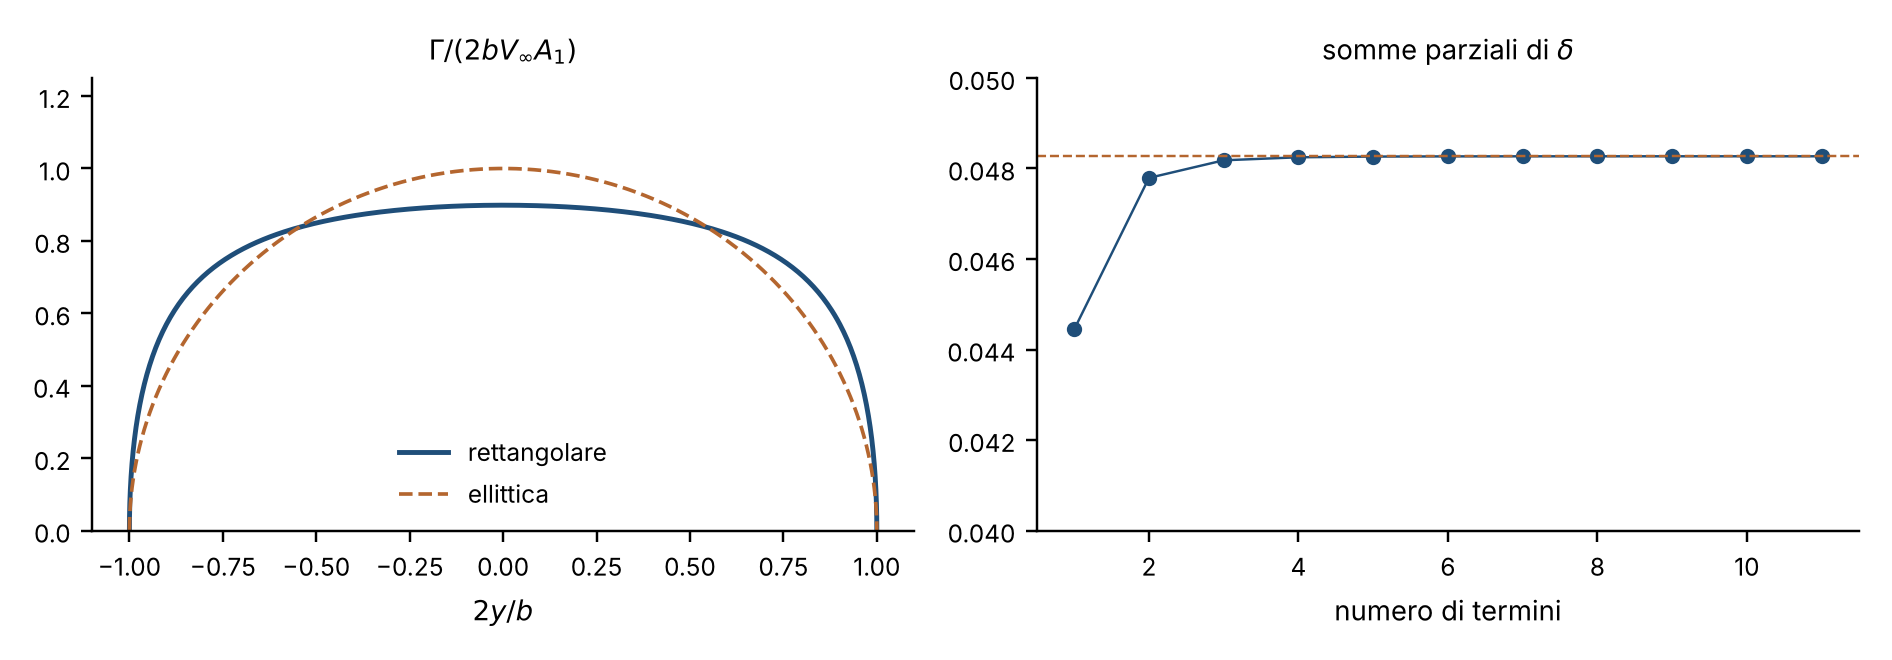
\includegraphics[width=\textwidth]{figure/resistenza_indotta.png}
\caption{A sinistra: la distribuzione di circolazione lungo l'apertura di un'ala
rettangolare con $AR=6$ (blu), confrontata con la distribuzione ellittica con la stessa
portanza (tratteggio rame). A destra: le somme parziali $\delta_{N}$ della serie
$\delta=\sum n(A_{n}/A_{1})^{2}$, crescenti e rapidamente convergenti, come deve accadere per
una serie convergente a termini non negativi (\texttt{python/fig\_resistenza\_indotta.py}).}
\label{fig:resistenza-indotta}
\end{figure}

\subsection{Approfondimento: prodotti infiniti e il prodotto di Wallis}
\label{subsec:prodotti-infiniti}

Come una serie è il limite delle somme dei suoi primi $n$ termini, così un \emph{prodotto
infinito} è il limite dei prodotti dei suoi primi $n$ fattori. Lo studio dei prodotti
infiniti si riconduce a quello delle serie, e conduce a una delle più antiche formule
per $\pi$.

\begin{definizione}[Prodotto infinito]\label{def:prodotto-infinito}
\index{prodotto infinito}
Sia $b_{k}>0$ per ogni $k\in\N$, e sia $p_{n}=b_{1}b_{2}\cdots b_{n}=\prod_{k=1}^{n}b_{k}$ il \emph{prodotto
parziale} $n$-esimo. Il prodotto infinito $\prod_{k=1}^{\infty}b_{k}$ si dice \emph{convergente} se
$p_{n}$ ha limite $P$ finito e \emph{positivo}, e allora si scrive $\prod_{k=1}^{\infty}b_{k}=P$; si
dice \emph{divergente} se $p_{n}\to+\infty$ oppure $p_{n}\to0$.
\end{definizione}

L'esclusione del limite $0$ è naturale. Passando ai logaritmi,
$\log p_{n}=\sum_{k=1}^{n}\log b_{k}$: se la serie $\sum\log b_{k}$ ha somma $L\in\R$, per la continuità
dell'esponenziale $p_{n}=e^{\log p_{n}}\to e^{L}>0$; viceversa, se $p_{n}\to P>0$, per la continuità del
logaritmo $\log p_{n}\to\log P$. Dunque \emph{il prodotto converge se e solo se converge la
serie dei logaritmi dei fattori}, e il caso $p_{n}\to0$ corrisponde a $\sum\log b_{k}=-\infty$. Come
per le serie, inoltre, se il prodotto converge i fattori $b_{n}=\frac{p_{n}}{p_{n-1}}$ tendono a
$\frac PP=1$: conviene scriverli nella forma $b_{k}=1+a_{k}$, con $a_{k}\to0$.

\begin{teorema}[Prodotti a fattori non minori di uno]\label{teo:prodotti-infiniti}
Sia $a_{k}\ge0$ per ogni $k$. Il prodotto $\prod_{k=1}^{\infty}(1+a_{k})$ converge se e solo se
converge la serie $\sum_{k=1}^{\infty}a_{k}$; altrimenti diverge a $+\infty$. Inoltre, dette $s_{n}$ e
$p_{n}$ le somme e i prodotti parziali,
\begin{equation}\label{eq:prodotti-stime}
  1+s_{n}\le p_{n}\le e^{s_{n}} \qquad\perogni n\in\N .
\end{equation}
\end{teorema}

\begin{schema}
\Ipotesi{$a_{k}\ge0$ per ogni $k$; \ $s_{n}=\sum_{k=1}^{n}a_{k}$, \ $p_{n}=\prod_{k=1}^{n}(1+a_{k})$.}
\Tesi{$1+s_{n}\le p_{n}\le e^{s_{n}}$; \ $\prod(1+a_{k})$ converge $\sse$ $\sum a_{k}<+\infty$; \
altrimenti $p_{n}\to+\infty$.}
\end{schema}

\begin{strategia}
Sviluppando il prodotto $(1+a_{1})\cdots(1+a_{n})$ si ottengono il termine $1$, tutti gli $a_{k}$ e
i loro prodotti, che sono non negativi: quindi $p_{n}\ge1+s_{n}$. La disuguaglianza
$1+x\le e^{x}$, applicata a ogni fattore, dà $p_{n}\le e^{a_{1}}\cdots e^{a_{n}}=e^{s_{n}}$. Le successioni $s_{n}$
e $p_{n}$ sono crescenti, e le due stime dicono che l'una è limitata se e solo se lo è
l'altra.
\end{strategia}

\begin{dimostrazione}
La prima delle \eqref{eq:prodotti-stime} si dimostra per induzione. Per $n=1$,
$p_{1}=1+a_{1}=1+s_{1}$. Se $p_{n}\ge1+s_{n}$, moltiplicando per $1+a_{n+1}>0$,
\[
  \begin{aligned}
  p_{n+1}&=p_{n}(1+a_{n+1})\ge(1+s_{n})(1+a_{n+1})\\
  &=1+s_{n+1}+s_{n}a_{n+1}\ge1+s_{n+1} .
  \end{aligned}
\]
Per la seconda, la \eqref{eq:exp-log-disuguaglianze} dà $0<1+a_{k}\le e^{a_{k}}$ per ogni $k$, e
moltiplicando membro a membro queste disuguaglianze tra numeri positivi
$p_{n}\le e^{a_{1}}e^{a_{2}}\cdots e^{a_{n}}=e^{s_{n}}$. La successione $p_{n}$ è crescente, perché
$p_{n+1}=p_{n}(1+a_{n+1})\ge p_{n}$, e $p_{n}\ge1$; per il \cref{teo:monotone} ha limite $P\in[1,+\infty]$.
Se $\sum a_{k}=s<+\infty$, allora $p_{n}\le e^{s_{n}}\le e^{s}$ e $P\in[1,e^{s}]$ è finito e positivo: il
prodotto converge. Se invece $s_{n}\to+\infty$, da $p_{n}\ge1+s_{n}$ e dal
\cref{teo:confronto-infinito} segue $p_{n}\to+\infty$.
\end{dimostrazione}

\begin{esempio}\label{es:prodotti-infiniti}
\begin{enumerate}[label=(\alph*)]
  \item Il prodotto $\prod_{k=1}^{\infty}\bigl(1+\frac1k\bigr)$ diverge: i fattori $\frac{k+1}k$ si semplificano «a
  cannocchiale» e $p_{n}=\frac21\cdot\frac32\cdots\frac{n+1}n=n+1$. La seconda delle \eqref{eq:prodotti-stime}
  diventa $n+1\le e^{H_{n}}$, cioè $H_{n}\ge\log(n+1)$: è la stima \eqref{eq:armonica-log}, che
  ritroviamo così per una quarta via.
  \item Il prodotto $\prod_{k=1}^{\infty}\bigl(1+\frac1{k^{2}}\bigr)$ converge, perché $\sum\frac1{k^{2}}$ converge, e per le
  \eqref{eq:prodotti-stime} il suo valore è compreso tra $1+\frac{\pi^{2}}6\approx2{,}64$ e
  $e^{\pi^{2}/6}\approx5{,}18$. (Il valore esatto è $\frac{e^{\pi}-e^{-\pi}}{2\pi}\approx3{,}68$.)
\end{enumerate}
\end{esempio}

Il prodotto infinito più celebre è quello di Wallis. I suoi fattori sono
$\frac{(2k)^{2}}{(2k-1)(2k+1)}=\frac{4k^{2}}{4k^{2}-1}=1+\frac1{4k^{2}-1}$, e poiché
$\frac1{4k^{2}-1}=\frac12\bigl(\frac1{2k-1}-\frac1{2k+1}\bigr)$, la serie $\sum\frac1{4k^{2}-1}$ è telescopica e
converge, con somma $\frac12$ (\cref{prop:serie-telescopica}): per il
\cref{teo:prodotti-infiniti} il prodotto converge, a un valore compreso tra $\frac32$ e
$e^{1/2}$. Il valore esatto viene dal calcolo integrale.

\begin{teorema}[Prodotto di Wallis]\label{teo:wallis}\index{prodotto di Wallis}
\begin{equation}\label{eq:wallis}
  \frac\pi2=\prod_{k=1}^{\infty}\frac{(2k)^{2}}{(2k-1)(2k+1)}
  =\frac21\cdot\frac23\cdot\frac43\cdot\frac45\cdot\frac65\cdot\frac67\cdots
\end{equation}
\end{teorema}

\begin{schema}
\Ipotesi{$I_{n}=\int_{0}^{\pi/2}\sen^{n}x\,dx$, con la formula di riduzione $I_{n}=\frac{n-1}nI_{n-2}$
per $n\ge2$ (\cref{es:wallis}); \ $W_{m}=\prod_{k=1}^{m}\frac{(2k)^{2}}{(2k-1)(2k+1)}$.}
\Tesi{$W_{m}\to\frac\pi2$.}
\end{schema}

\begin{strategia}
Iterando la formula di riduzione a partire da $I_{0}=\frac\pi2$ e $I_{1}=1$, l'integrale di indice
pari $I_{2m}$ contiene il fattore $\frac\pi2$ e quello di indice dispari $I_{2m+1}$ no, e il loro
rapporto risulta proprio $\frac\pi{2W_{m}}$. D'altra parte, poiché $0\le\sen x\le1$, le potenze
di $\sen x$ decrescono al crescere dell'esponente, e così i loro integrali:
$I_{2m+1}\le I_{2m}\le I_{2m-1}$. Questa catena intrappola il rapporto tra $1$ e $\frac{2m+1}{2m}$, che
tende a $1$, e il teorema dei carabinieri conclude.
\end{strategia}

\begin{dimostrazione}
Applicando $m$ volte la formula di riduzione (formalmente, per induzione su $m$),
\[
  I_{2m}=\frac{2m-1}{2m}\cdot\frac{2m-3}{2m-2}\cdots\frac12\cdot\frac\pi2 ,\qquad
  I_{2m+1}=\frac{2m}{2m+1}\cdot\frac{2m-2}{2m-1}\cdots\frac23\cdot1 .
\]
In particolare $I_{2m+1}>0$, e dividendo
\[
  \frac{I_{2m}}{I_{2m+1}}=\frac\pi2\prod_{k=1}^{m}\frac{2k-1}{2k}\cdot\prod_{k=1}^{m}\frac{2k+1}{2k}
  =\frac\pi2\prod_{k=1}^{m}\frac{(2k-1)(2k+1)}{(2k)^{2}}=\frac\pi{2W_{m}} .
\]
Per $x\in[0,\frac\pi2]$ si ha $0\le\sen x\le1$, e quindi
$\sen^{2m+1}x\le\sen^{2m}x\le\sen^{2m-1}x$; per il confronto tra integrali
(\cref{teo:confronto-integrali}), $I_{2m+1}\le I_{2m}\le I_{2m-1}$. Dividendo per $I_{2m+1}$ e usando la
formula di riduzione con $n=2m+1$, cioè $I_{2m-1}=\frac{2m+1}{2m}I_{2m+1}$, si ottiene
\[
  1\le\frac\pi{2W_{m}}\le\frac{2m+1}{2m}=1+\frac1{2m} \qquad\perogni m\in\N .
\]
Per il teorema dei carabinieri (\cref{teo:carabinieri}) $\frac\pi{2W_{m}}\to1$, e dunque
$W_{m}\to\frac\pi2$ (\cref{teo:operazioni-limiti}).
\end{dimostrazione}

L'ultima catena di disuguaglianze dice anche che
$0\le\frac\pi2-W_{m}\le\frac\pi2\bigl(1-\frac{2m}{2m+1}\bigr)=\frac\pi{2(2m+1)}$: l'errore è dell'ordine di $\frac1m$,
e la convergenza è lentissima. Il programma che segue mostra che ogni volta che il
numero dei fattori si moltiplica per dieci si guadagna una sola cifra esatta: il
prodotto $m\bigl(\frac\pi2-W_{m}\bigr)$ si stabilizza attorno a $\frac\pi8\approx0{,}3927$, cioè
$\frac\pi2-W_{m}\approx\frac\pi{8m}$, in accordo con la maggiorazione $\frac\pi{2(2m+1)}\approx\frac\pi{4m}$. Il
prodotto di Wallis non è dunque un metodo per calcolare $\pi$, ma un ponte tra il mondo
discreto dei prodotti di numeri interi e quello continuo degli integrali, che ritorna
nel calcolo delle probabilità e nella formula di Stirling per $n!$.

\needspace{14\baselineskip}
\begin{python}[La lenta convergenza del prodotto di Wallis]
import math

W = 1.0                                   # prodotto parziale W_m
for m in range(1, 10**6 + 1):
    W *= 4 * m * m / (4 * m * m - 1)
    if m in (10, 100, 1000, 10**4, 10**5, 10**6):
        err = math.pi / 2 - W
        print(f"m = {m:>7}: W_m = {W:.9f}  errore = {err:.2e}"
              f"  m*errore = {m * err:.5f}")
print(f"pi/2 = {math.pi / 2:.9f},  pi/8 = {math.pi / 8:.5f}")
\end{python}
\begin{risultato}
m =      10: W_m = 1.533851903  errore = 3.69e-02  m*errore = 0.36944
m =     100: W_m = 1.566893745  errore = 3.90e-03  m*errore = 0.39026
m =    1000: W_m = 1.570403873  errore = 3.92e-04  m*errore = 0.39245
m =   10000: W_m = 1.570757059  errore = 3.93e-05  m*errore = 0.39267
m =  100000: W_m = 1.570792400  errore = 3.93e-06  m*errore = 0.39270
m = 1000000: W_m = 1.570795934  errore = 3.93e-07  m*errore = 0.39270
pi/2 = 1.570796327,  pi/8 = 0.39270
\end{risultato}

\begin{notastorica}[Viète, Wallis, Brouncker, Newton]
Il primo prodotto infinito della storia è di François Viète (1593), che ottenne $\frac2\pi$
come prodotto di radici quadrate annidate studiando i poligoni regolari inscritti nel
cerchio. Il prodotto \eqref{eq:wallis} fu trovato da John Wallis, professore di geometria a
Oxford, nell'\emph{Arithmetica infinitorum} (1656), cercando l'area del quarto di cerchio,
cioè $\int_{0}^{1}\sqrt{1-x^{2}}\,dx=\frac\pi4$. Wallis sapeva calcolare gli integrali di $(1-x^{2})^{n}$ per
$n$ intero e ne «interpolò» il valore per $n=\frac12$, supponendo che la regolarità osservata
continuasse: un procedimento audace e senza dimostrazione, che il nostro
\cref{teo:wallis} giustifica a posteriori. Lord William Brouncker, futuro primo
presidente della Royal Society, trasformò il risultato in una frazione continua per
$\frac4\pi$, pubblicata nella stessa opera. Nell'inverno 1664--65 il giovane Isaac Newton
studiò l'\emph{Arithmetica infinitorum} e, applicando l'interpolazione di Wallis agli
integrali di $(1-t^{2})^{n}$ tra $0$ e un estremo variabile $x$, scoprì la serie binomiale
per esponenti frazionari (nota storica del \S\ref{sec:serie-taylor}). Circa ottant'anni
dopo il prodotto ricomparve come caso particolare di una scoperta di Eulero, la
scrittura del seno come prodotto infinito,
$\sen x=x\prod_{k=1}^{\infty}\bigl(1-\frac{x^{2}}{k^{2}\pi^{2}}\bigr)$, con cui nel 1734 egli ricavò la somma
$\frac{\pi^{2}}6$: con $x=\frac\pi2$ se ne ottiene proprio il prodotto di Wallis.
\end{notastorica}

%% ----------------------------------------------------------------------------
%%  §11.7  Serie alternate
%% ----------------------------------------------------------------------------
\section{Serie alternate}
\label{sec:serie-alternate}

Finora abbiamo studiato quasi esclusivamente serie a termini non negativi. Eliminiamo
questa restrizione, cominciando dalle \emph{serie alternate}\index{serie!alternata},
cioè le serie del tipo
\begin{equation}\label{eq:serie-alternata}
  \sum_{k=1}^{\infty}(-1)^{k-1}a_{k}=a_{1}-a_{2}+a_{3}-a_{4}+\dots+(-1)^{n-1}a_{n}+\cdots, \qquad a_{n}\ge0 ,
\end{equation}
in cui i termini cambiano segno a ogni passo. L'esempio tipico è la \emph{serie armonica
alternata}
\begin{equation}\label{eq:armonica-alternata}
  \sum_{k=1}^{\infty}\frac{(-1)^{k-1}}k=1-\frac12+\frac13-\frac14+\cdots ,
\end{equation}
che, a differenza della serie armonica, converge. Il meccanismo è visibile nella
\cref{fig:alternata}: ogni termine «corregge» il precedente con una correzione più
piccola, e le somme parziali oscillano attorno alla somma con oscillazioni sempre più
strette. Ci servirà un semplice lemma sulle successioni.

\begin{lemma}\label{lem:pari-dispari}
Se le estratte di indici pari $s_{2k}$ e di indici dispari $s_{2k+1}$ di una successione
$s_{n}$ convergono allo stesso limite $s$, allora $s_{n}\to s$.
\end{lemma}

\begin{schema}
\Ipotesi{$s_{2k}\to s$ \ e \ $s_{2k+1}\to s$ per $k\to+\infty$, con $s\in\R$.}
\Tesi{$s_{n}\to s$.}
\end{schema}

\begin{strategia}
Ogni indice $n$ è pari o dispari. Fissato $\epsilon>0$, le due estratte entrano
definitivamente nell'intorno $(s-\epsilon,s+\epsilon)$, ciascuna da un proprio indice in poi: basta
prendere il più grande dei due indici, tradotto in termini di $n$.
\end{strategia}

\begin{dimostrazione}
Sia $\epsilon>0$. Esistono $k_{1}$ e $k_{2}$ tali che $\abs{s_{2k}-s}<\epsilon$ per $k>k_{1}$ e
$\abs{s_{2k+1}-s}<\epsilon$ per $k>k_{2}$. Posto $\nu=2\max\{k_{1},k_{2}\}+1$, ogni $n>\nu$ è della forma
$2k$ con $k>k_{1}$ oppure $2k+1$ con $k>k_{2}$, e in entrambi i casi $\abs{s_{n}-s}<\epsilon$.
\end{dimostrazione}

\begin{teorema}[Criterio di Leibniz]\label{teo:leibniz}\index{criterio di Leibniz}
Sia $a_{n}\ge0$ una successione decrescente e infinitesima. Allora la serie alternata
\eqref{eq:serie-alternata} è convergente. Inoltre, detta $s$ la sua somma e $s_{n}$ la
somma parziale $n$-esima, si ha
\begin{equation}\label{eq:stima-leibniz}
  \abs{s_{n}-s}\le a_{n+1} \qquad\perogni n\in\N ,
\end{equation}
e la somma $s$ è compresa tra due somme parziali consecutive qualsiasi.
\end{teorema}

\begin{schema}
\Ipotesi{$a_{n}\ge0$; \ $a_{n+1}\le a_{n}$ per ogni $n$; \ $a_{n}\to0$.}
\Tesi{$\sum(-1)^{k-1}a_{k}$ converge; \ $\abs{s_{n}-s}\le a_{n+1}$.}
\end{schema}

\begin{strategia}
Separiamo le somme parziali di indice pari da quelle di indice dispari. Passando da
$s_{2k}$ a $s_{2k+2}$ si aggiunge $a_{2k+1}-a_{2k+2}\ge0$: le somme pari crescono. Passando da
$s_{2k-1}$ a $s_{2k+1}$ si aggiunge $-a_{2k}+a_{2k+1}\le0$: le somme dispari decrescono. Inoltre
ogni somma dispari supera ogni somma pari. Abbiamo due successioni monotòne e
limitate, una che sale e una che scende, la cui distanza $a_{2k+1}$ tende a zero: come in una
successione di intervalli incapsulati, convergono allo stesso limite, che è compreso tra
loro. La stima dell'errore segue proprio da questo «incapsulamento».
\end{strategia}

\begin{dimostrazione}
Per ogni $k\in\N$, poiché $a_{n}$ è decrescente,
\begin{align}
  s_{2k+2}&=s_{2k}+(a_{2k+1}-a_{2k+2})\ge s_{2k} , \label{eq:leibniz-pari}\\
  s_{2k+1}&=s_{2k-1}-(a_{2k}-a_{2k+1})\le s_{2k-1} . \label{eq:leibniz-dispari}
\end{align}
Dunque $s_{2}\le s_{4}\le s_{6}\le\cdots$ e $s_{1}\ge s_{3}\ge s_{5}\ge\cdots$. Inoltre
$s_{2k+1}-s_{2k}=a_{2k+1}\ge0$, e quindi
\begin{equation}\label{eq:leibniz-incapsulati}
  s_{2}\le s_{2k}\le s_{2k+1}\le s_{1} \qquad\perogni k\in\N .
\end{equation}
La successione $s_{2k}$ è crescente e limitata superiormente da $s_{1}$, la successione
$s_{2k+1}$ è decrescente e limitata inferiormente da $s_{2}$; per il teorema sulle successioni
monotòne (\cref{teo:monotone}) esse convergono, a limiti $s'$ e $s''$. Passando al limite
in $s_{2k+1}-s_{2k}=a_{2k+1}$ si ottiene $s''-s'=0$, perché $a_{n}\to0$. Per il
\cref{lem:pari-dispari} la serie converge, e la sua somma è $s=s'=s''$.

Per il teorema sulle successioni monotòne, inoltre, $s=\sup_{k}s_{2k}=\inf_{k}s_{2k+1}$, e quindi
$s_{2k}\le s\le s_{2k+1}$ e $s\le s_{2k-1}$ per ogni $k$. Ne segue
\begin{align*}
  0&\le s-s_{2k}\le s_{2k+1}-s_{2k}=a_{2k+1} ,\\
  0&\le s_{2k+1}-s\le s_{2k+1}-s_{2k+2}=a_{2k+2} ,
\end{align*}
cioè $\abs{s_{n}-s}\le a_{n+1}$ sia per $n=2k$ sia per $n=2k+1$; per $n=1$ la stessa disuguaglianza
segue da $s_{2}\le s\le s_{1}$. Le disuguaglianze $s_{2k}\le s\le s_{2k\pm1}$ dicono anche che $s$ è
compresa tra due somme parziali consecutive.
\end{dimostrazione}

La \eqref{eq:stima-leibniz} si enuncia spesso così: \emph{per una serie alternata che
verifica le ipotesi del criterio di Leibniz, l'errore che si commette sostituendo alla
somma la somma dei primi $n$ termini è maggiorato, in valore assoluto, dal primo termine
trascurato}. Si sa anche il segno dell'errore: è quello del primo termine trascurato.

\begin{esempio}[La serie armonica alternata]\label{es:armonica-alternata}
La successione $a_{n}=\frac1n$ è positiva, decrescente e infinitesima: la serie
\eqref{eq:armonica-alternata} converge. Quanti termini occorre sommare per avere
$\abs{s-s_{n}}\le\frac1{100}$? Per la \eqref{eq:stima-leibniz} basta che $a_{n+1}=\frac1{n+1}\le\frac1{100}$,
cioè $n\ge99$. Il valore della somma si ottiene dallo sviluppo del logaritmo: nel
\S\ref{sec:taylor-peano} abbiamo visto che
$\log(1+x)=\sum_{k=1}^{n}\frac{(-1)^{k-1}}kx^{k}+R(x)$ con $\abs{R(x)}\le\frac{x^{n+1}}{n+1}$ per $x\ge0$. Con
$x=1$, $\abs{\log2-s_{n}}\le\frac1{n+1}\to0$, e dunque
\begin{equation}\label{eq:somma-log2}
  1-\frac12+\frac13-\frac14+\dots=\log2=0{,}693147\ldots
\end{equation}
Allo stesso modo la serie di Leibniz \eqref{eq:serie-leibniz},
$1-\frac13+\frac15-\cdots=\frac\pi4$, verifica le ipotesi del criterio, e la stima
$\abs{s_{n}-\frac\pi4}\le\frac1{2n+1}$ ritrova quella del \cref{cap:taylor}.
\end{esempio}

\begin{attenzione}
L'ipotesi che $a_{n}$ sia \emph{decrescente} non si può omettere. Si consideri la serie
alternata con $a_{2j-1}=\frac1j$ e $a_{2j}=\frac1{4j^{2}}$:
\[
  1-\frac14+\frac12-\frac1{16}+\frac13-\frac1{36}+\cdots .
\]
I termini tendono a zero, ma non in modo monotòno. Le somme parziali di indice pari sono
$s_{2m}=\sum_{j=1}^{m}\bigl(\frac1j-\frac1{4j^{2}}\bigr)=H_{m}-\frac14\sum_{j=1}^{m}\frac1{j^{2}}$, che tende a $+\infty$
perché $H_{m}\to+\infty$ mentre $\sum\frac1{j^{2}}$ converge. Anche $s_{2m+1}=s_{2m}+\frac1{m+1}>s_{2m}$ tende a
$+\infty$, e per il \cref{lem:pari-dispari} (che vale, con la stessa dimostrazione e con gli
intorni di $+\infty$ al posto di quelli di $s$, anche per limiti infiniti) la serie diverge.
\end{attenzione}

\begin{figure}[htb]
\centering
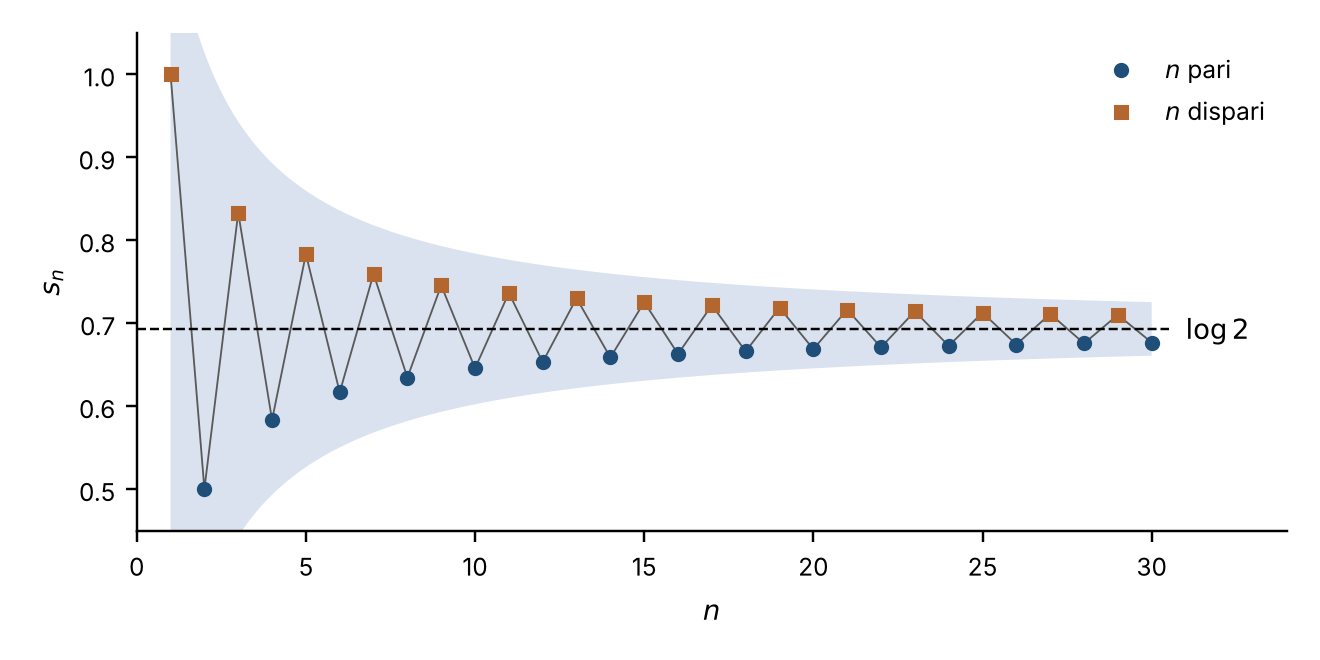
\includegraphics[width=\textwidth]{figure/alternata.png}
\caption{Le somme parziali della serie armonica alternata (punti) oscillano attorno alla
somma $\log2$: quelle di indice pari crescono, quelle di indice dispari decrescono, e la
somma è sempre compresa tra due somme consecutive. La fascia grigia ha semiampiezza
$a_{n+1}=\frac1{n+1}$, la stima dell'errore del criterio di Leibniz
(\texttt{python/fig\_alternata.py}).}
\label{fig:alternata}
\end{figure}

\needspace{10\baselineskip}
\begin{python}[La serie armonica alternata]
import math

s, err_max = 0.0, 0.0
for n in range(1, 10001):
    s += (-1)**(n - 1) / n
    errore = abs(s - math.log(2))
    err_max = max(err_max, errore * (n + 1))   # errore / a_(n+1)
    if n in (10, 99, 100, 1000, 10000):
        print(f"n = {n:5d}: s_n = {s:.8f}  errore = {errore:.2e}"
              f"  a_(n+1) = {1/(n+1):.2e}")
print(f"max di |s_n - log 2| / a_(n+1) = {err_max:.4f}  (<= 1)")
\end{python}
\begin{risultato}
n =    10: s_n = 0.64563492  errore = 4.75e-02  a_(n+1) = 9.09e-02
n =    99: s_n = 0.69817218  errore = 5.02e-03  a_(n+1) = 1.00e-02
n =   100: s_n = 0.68817218  errore = 4.98e-03  a_(n+1) = 9.90e-03
n =  1000: s_n = 0.69264743  errore = 5.00e-04  a_(n+1) = 9.99e-04
n = 10000: s_n = 0.69309718  errore = 5.00e-05  a_(n+1) = 1.00e-04
max di |s_n - log 2| / a_(n+1) = 0.6137  (<= 1)
\end{risultato}

%% ----------------------------------------------------------------------------
%%  §11.8  Convergenza assoluta
%% ----------------------------------------------------------------------------
\section{Convergenza assoluta}
\label{sec:convergenza-assoluta}

Per una serie a termini di segno qualsiasi, il primo passo è spesso studiare la serie
dei valori assoluti, che è a termini non negativi e alla quale si applicano tutti i
criteri del \S\ref{sec:criteri-convergenza}.

\begin{definizione}[Convergenza assoluta]\label{def:convergenza-assoluta}
\index{serie!assolutamente convergente}
La serie $\sum a_{k}$ si dice \emph{assolutamente convergente} se è convergente la serie dei
valori assoluti
\begin{equation}\label{eq:serie-valori-assoluti}
  \sum_{k=1}^{\infty}\abs{a_{k}}=\abs{a_{1}}+\abs{a_{2}}+\dots+\abs{a_{n}}+\cdots .
\end{equation}
\end{definizione}

Una serie convergente non è necessariamente assolutamente convergente: la serie armonica
alternata converge, ma la serie dei suoi valori assoluti è la serie armonica, che
diverge. Una serie convergente ma non assolutamente convergente si dice
\emph{semplicemente} (o \emph{condizionatamente}) convergente. Il viceversa, invece, vale.

\begin{teorema}[La convergenza assoluta implica la convergenza]
\label{teo:convergenza-assoluta}
Una serie assolutamente convergente è convergente, e
\begin{equation}\label{eq:disuguaglianza-serie}
  \Bigl|\sum_{k=1}^{\infty}a_{k}\Bigr|\le\sum_{k=1}^{\infty}\abs{a_{k}} .
\end{equation}
\end{teorema}

\needspace{9\baselineskip}
\begin{schema}
\Ipotesi{$\sum\abs{a_{k}}<+\infty$.}
\Tesi{$\sum a_{k}$ converge e $\abs{\sum a_{k}}\le\sum\abs{a_{k}}$.}
\end{schema}

\begin{strategia}
Non conosciamo la somma della serie, e quindi conviene un criterio che non la richieda:
quello di Cauchy. I blocchi di termini consecutivi della serie data sono, per la
disuguaglianza triangolare, più piccoli dei corrispondenti blocchi della serie dei valori
assoluti, che verificano la condizione di Cauchy perché questa serie converge. Daremo
anche una seconda dimostrazione, che riconduce il problema a serie a termini non
negativi.
\end{strategia}

\begin{dimostrazione}[Prima dimostrazione (con il criterio di Cauchy)]
Poiché $\sum\abs{a_{k}}$ converge, per il criterio di Cauchy (\cref{teo:cauchy-serie}), dato
$\epsilon>0$ esiste $\nu$ tale che $\sum_{k=n+1}^{n+p}\abs{a_{k}}<\epsilon$ per ogni $n>\nu$ e ogni $p\in\N$. Per gli
stessi indici, per la disuguaglianza triangolare,
\[
  \Bigl|\sum_{k=n+1}^{n+p}a_{k}\Bigr|\le\sum_{k=n+1}^{n+p}\abs{a_{k}}<\epsilon ,
\]
e quindi, ancora per il criterio di Cauchy, la serie $\sum a_{k}$ converge. Infine, per
ogni $n$, $\abs{\sum_{k=1}^{n}a_{k}}\le\sum_{k=1}^{n}\abs{a_{k}}$; passando al limite (il valore assoluto è
continuo e le disuguaglianze larghe si conservano) si ottiene la
\eqref{eq:disuguaglianza-serie}.
\end{dimostrazione}

\begin{dimostrazione}[Seconda dimostrazione (con il confronto)]
Per ogni $k$ si ha $0\le a_{k}+\abs{a_{k}}\le2\abs{a_{k}}$. La serie di termine generale $2\abs{a_{k}}$
converge, e per il criterio del confronto converge anche la serie a termini non negativi
$\sum(a_{k}+\abs{a_{k}})$. Allora, per la linearità (\cref{prop:linearita-serie}), converge
anche la serie
\[
  \sum_{k=1}^{\infty}a_{k}=\sum_{k=1}^{\infty}\bigl(a_{k}+\abs{a_{k}}\bigr)-\sum_{k=1}^{\infty}\abs{a_{k}} ,
\]
differenza di due serie convergenti. La \eqref{eq:disuguaglianza-serie} si dimostra come
nella prima dimostrazione.
\end{dimostrazione}

Applicando i criteri del \S\ref{sec:criteri-convergenza} alla serie dei valori assoluti si
ottengono criteri di convergenza per serie a termini di segno qualsiasi. Ad esempio, dai
criteri del rapporto e della radice:

\begin{corollario}\label{cor:rapporto-assoluto}
Sia $a_{n}\neq0$ e supponiamo che esista $\ell=\lim\frac{\abs{a_{n+1}}}{\abs{a_{n}}}$ oppure
$\ell=\lim\sqrt[n]{\abs{a_{n}}}$. Se $\ell<1$ la serie $\sum a_{k}$ converge assolutamente; se $\ell>1$ la
serie non converge.
\end{corollario}

\begin{schema}
\Ipotesi{$a_{n}\neq0$; \ $\frac{\abs{a_{n+1}}}{\abs{a_{n}}}\to\ell$ oppure $\sqrt[n]{\abs{a_{n}}}\to\ell$.}
\Tesi{$\ell<1\implica\sum a_{k}$ assolutamente convergente; \ $\ell>1\implica\sum a_{k}$ non converge.}
\end{schema}

\begin{strategia}
Si applicano i criteri del rapporto e della radice alla serie dei valori assoluti. Per
$\ell<1$ si conclude con il teorema appena dimostrato; per $\ell>1$ si riutilizza ciò che le
dimostrazioni di quei criteri hanno mostrato: il termine generale non tende a zero.
\end{strategia}

\begin{dimostrazione}
Se $\ell<1$, la serie $\sum\abs{a_{k}}$ converge per il \cref{teo:criterio-rapporto-serie} o per il
\cref{teo:criterio-radice}, e si applica il \cref{teo:convergenza-assoluta}. Se $\ell>1$, nelle
dimostrazioni di quei criteri abbiamo visto che $\abs{a_{n}}$ non tende a zero; allora neppure
$a_{n}$ tende a zero, e la serie non converge per il \cref{teo:condizione-necessaria}.
\end{dimostrazione}

\begin{esempio}\label{es:assoluta}
\begin{enumerate}[label=(\alph*)]
  \item $\sum\frac{\sen k}{k^{2}}$ converge assolutamente, perché $\frac{\abs{\sen k}}{k^{2}}\le\frac1{k^{2}}$. I segni dei
  suoi termini non seguono alcuno schema regolare: il criterio di Leibniz non sarebbe
  applicabile.
  \item La serie esponenziale $\sum\frac{x^{k}}{k!}$ converge assolutamente per \emph{ogni}
  $x\in\R$: il rapporto dei valori assoluti è $\frac{\abs x}{n+1}\to0$.
  \item $\sum\frac{(-1)^{k}}{\sqrt k}$ converge per il criterio di Leibniz, ma non assolutamente,
  perché $\sum\frac1{\sqrt k}$ diverge ($p=\frac12$).
\end{enumerate}
\end{esempio}

\subsection{Riordinare una serie}

In una somma finita l'ordine degli addendi è irrilevante. Per le serie la questione è
delicata, perché la somma è un limite, e il limite dipende dall'ordine in cui si
presentano le somme parziali. Un \emph{riordinamento} della serie $\sum a_{k}$ è una serie
$\sum a_{\sigma(k)}$, dove $\sigma:\N\to\N$ è una funzione biunivoca: gli stessi termini, ciascuno
preso una e una sola volta, in un ordine diverso.

\begin{teorema}[di Dirichlet]\label{teo:dirichlet-riordinamento}
\index{teorema!di Dirichlet sui riordinamenti}
Se la serie $\sum a_{k}$ è assolutamente convergente, ogni suo riordinamento è
assolutamente convergente e ha la stessa somma.
\end{teorema}

\begin{schema}
\Ipotesi{$\sum\abs{a_{k}}<+\infty$; \ $\sigma:\N\to\N$ biunivoca.}
\Tesi{$\sum a_{\sigma(k)}$ converge assolutamente e $\sum_{k=1}^{\infty}a_{\sigma(k)}=\sum_{k=1}^{\infty}a_{k}$.}
\end{schema}

\begin{strategia}
Per le serie a termini non negativi la somma è l'estremo superiore delle somme parziali,
e ogni somma parziale della serie riordinata è maggiorata da una somma parziale della
serie data (basta prendere abbastanza termini da includere tutti quelli usati): dunque la
somma riordinata non supera quella originale, e per simmetria vale anche il viceversa.
Il caso generale si riconduce a questo scrivendo ogni termine come differenza della sua
parte positiva e della sua parte negativa.
\end{strategia}

\begin{dimostrazione}
\emph{Primo passo: $a_{k}\ge0$.} Sia $s=\sum a_{k}$ e sia $t_{n}=\sum_{k=1}^{n}a_{\sigma(k)}$. Posto
$N=\max\{\sigma(1),\dots,\sigma(n)\}$, gli indici $\sigma(1),\dots,\sigma(n)$ sono distinti e compresi tra $1$ e $N$,
e poiché i termini sono non negativi $t_{n}\le\sum_{j=1}^{N}a_{j}\le s$. Dunque la serie riordinata, a
termini non negativi, converge (\cref{teo:serie-positive}) e la sua somma $t$ verifica
$t\le s$. Ma la serie data è a sua volta un riordinamento di quella riordinata (mediante
la funzione inversa $\sigma^{-1}$), e lo stesso ragionamento dà $s\le t$. Quindi $t=s$.

\emph{Secondo passo: caso generale.} Poniamo $a_{k}^{+}=\max\{a_{k},0\}$ e $a_{k}^{-}=\max\{-a_{k},0\}$, in modo
che $a_{k}=a_{k}^{+}-a_{k}^{-}$ e $\abs{a_{k}}=a_{k}^{+}+a_{k}^{-}$. Poiché $0\le a_{k}^{\pm}\le\abs{a_{k}}$, le serie $\sum a_{k}^{+}$ e
$\sum a_{k}^{-}$ convergono per il confronto. Per il primo passo, applicato alle serie
$\sum\abs{a_{k}}$, $\sum a_{k}^{+}$ e $\sum a_{k}^{-}$, i loro riordinamenti convergono alle stesse somme; in
particolare $\sum a_{\sigma(k)}$ converge assolutamente e, per la linearità,
\[
  \sum_{k=1}^{\infty}a_{\sigma(k)}=\sum_{k=1}^{\infty}a_{\sigma(k)}^{+}-\sum_{k=1}^{\infty}a_{\sigma(k)}^{-}
  =\sum_{k=1}^{\infty}a_{k}^{+}-\sum_{k=1}^{\infty}a_{k}^{-}=\sum_{k=1}^{\infty}a_{k} . \qedhere
\]
\end{dimostrazione}

Per le serie semplicemente convergenti la situazione è opposta, e sorprendente.

\begin{esempio}[Un riordinamento della serie armonica alternata]\label{es:riordinamento}
Sia $L=\log2=1-\frac12+\frac13-\frac14+\cdots$. Moltiplicando per $\frac12$ (\cref{prop:linearita-serie})
e intercalando degli zeri, il che non cambia né il carattere né la somma
(\cref{oss:termini-nulli}),
\[
  \tfrac12L=0+\tfrac12+0-\tfrac14+0+\tfrac16+0-\tfrac18+\cdots .
\]
Sommando termine a termine con la serie di $L$, ancora per la linearità,
\[
  \tfrac32L=1+0+\tfrac13-\tfrac12+\tfrac15+0+\tfrac17-\tfrac14+\cdots ,
\]
e, togliendo gli zeri (ancora per l'\cref{oss:termini-nulli}),
\begin{equation}\label{eq:riordinamento}
  1+\frac13-\frac12+\frac15+\frac17-\frac14+\frac19+\frac1{11}-\frac16+\dots=\frac32\log2 .
\end{equation}
Il primo membro contiene esattamente i termini della serie armonica alternata, ciascuno
una volta, in un ordine diverso (due positivi e un negativo): è un suo riordinamento, ma
la somma è aumentata del $50\%$ (\cref{fig:riordinamento}).
\end{esempio}

Il fenomeno è del tutto generale, come dimostrò Riemann; ci limitiamo a enunciare il
risultato e a descrivere l'idea della dimostrazione.

\begin{teorema}[di Riemann, senza dimostrazione]\label{teo:riemann-riordinamento}
\index{teorema!di Riemann sui riordinamenti}
Se la serie $\sum a_{k}$ è semplicemente convergente, per ogni $L\in\overline\R$ esiste un suo
riordinamento che ha somma $L$; esistono inoltre riordinamenti indeterminati.
\end{teorema}

\begin{schema}
\Ipotesi{$\sum a_{k}$ convergente; \ $\sum\abs{a_{k}}=+\infty$; \ $L\in\overline\R$.}
\Tesi{esiste $\sigma:\N\to\N$ biunivoca con $\sum_{k=1}^{\infty}a_{\sigma(k)}=L$; \ esistono
riordinamenti indeterminati.}
\end{schema}

\begin{strategia}[Idea della dimostrazione]
Le serie $\sum a_{k}^{+}$ delle parti positive e $\sum a_{k}^{-}$ delle parti negative sono entrambe
divergenti (se una convergesse, convergerebbe anche l'altra, e quindi la serie dei valori
assoluti), mentre $a_{k}\to0$. Per ottenere la somma $L\in\R$ si prendono termini positivi
finché la somma parziale supera $L$, poi termini negativi finché scende sotto $L$, e così
via: le risorse non si esauriscono mai, perché ciascuna delle due serie diverge, e le
oscillazioni attorno a $L$ sono maggiorate dagli ultimi termini usati, che tendono a zero.
\end{strategia}

Il programma che segue mette in pratica questo algoritmo.

\begin{figure}[htb]
\centering
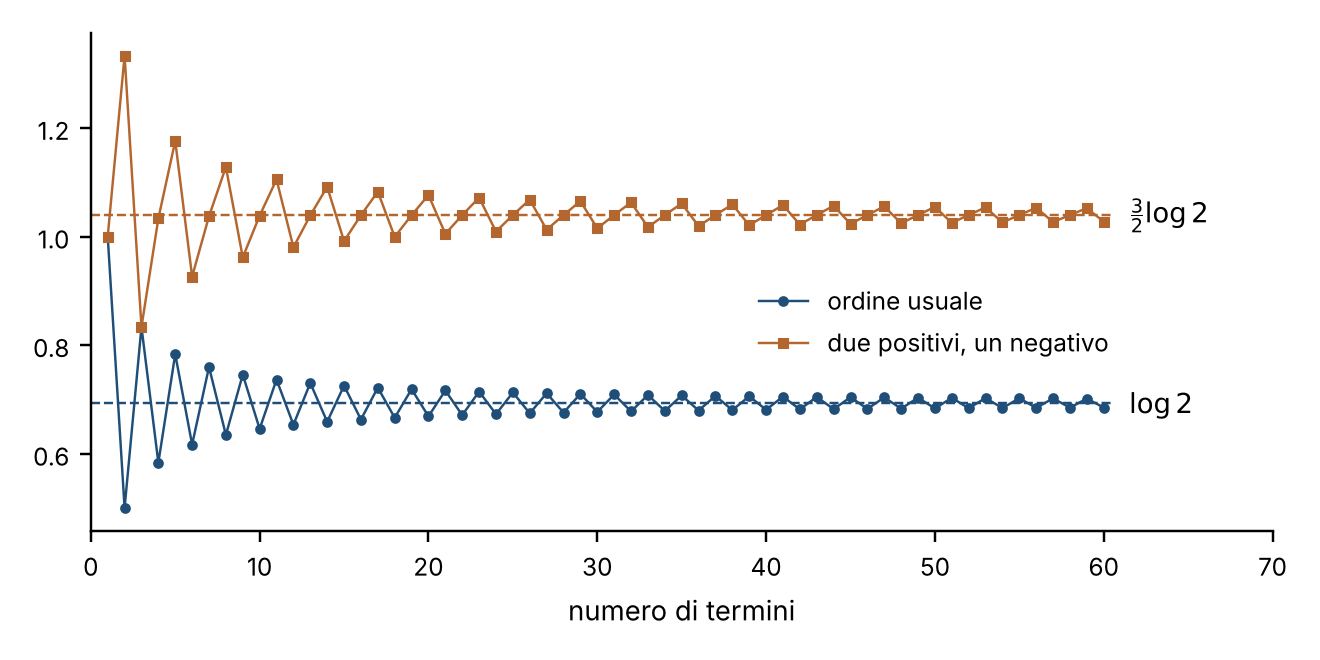
\includegraphics[width=\textwidth]{figure/riordinamento.png}
\caption{Somme parziali della serie armonica alternata nell'ordine usuale (blu), che
convergono a $\log2$, e del riordinamento \eqref{eq:riordinamento} con due termini positivi
e uno negativo (rame), che convergono a $\frac32\log2$. Gli stessi termini, sommati in un
ordine diverso, danno una somma diversa (\texttt{python/fig\_riordinamento.py}).}
\label{fig:riordinamento}
\end{figure}

\needspace{10\baselineskip}
\begin{python}[Riordinamenti della serie armonica alternata]
import math

def riordina(L, N):
    """Somma N termini di 1 - 1/2 + 1/3 - ... riordinati in modo
    che le somme parziali tendano a L (algoritmo di Riemann)."""
    s, p, q = 0.0, 1, 2          # prossimo dispari, prossimo pari
    for _ in range(N):
        if s <= L:
            s += 1 / p; p += 2   # termine positivo
        else:
            s -= 1 / q; q += 2   # termine negativo
    return s

s, p, q = 0.0, 1, 2              # due positivi e un negativo
for _ in range(100000):
    s += 1 / p + 1 / (p + 2) - 1 / q
    p, q = p + 4, q + 2
print(f"due +, un -:  {s:.6f}   (3/2) log 2 = {1.5*math.log(2):.6f}")
for L in (0.0, 1.0, math.pi):
    print(f"obiettivo L = {L:.6f}:  "
          f"somma = {riordina(L, 10**6):.6f}")
\end{python}
\begin{risultato}
due +, un -:  1.039718   (3/2) log 2 = 1.039721
obiettivo L = 0.000000:  somma = -0.000000
obiettivo L = 1.000000:  somma = 1.000000
obiettivo L = 3.141593:  somma = 3.141585
\end{risultato}

\begin{osservazione}
Il teorema di Dirichlet ha una conseguenza pratica: i termini di una serie
assolutamente convergente si possono raggruppare e riordinare nel modo più conveniente
senza alterare la somma, ad esempio sommando separatamente i termini positivi e quelli
negativi, o calcolando a parte certi blocchi di termini di cui si conosce la somma. Per
una serie semplicemente convergente, invece, l'ordine dei termini fa parte della
definizione stessa della serie. (Un'altra cosa è l'ordine in cui il calcolatore esegue
le addizioni di una somma parziale, che è una somma \emph{finita}: lì sommare dal termine
più piccolo al più grande riduce gli errori di arrotondamento, senza bisogno di alcun
teorema.)
\end{osservazione}

\begin{notastorica}[Cauchy, Dirichlet, Riemann]
Per tutto il Settecento le serie furono usate con grande disinvoltura, e talvolta con
risultati contraddittori. Fu Augustin-Louis Cauchy, nel \emph{Cours d'analyse} del 1821, a
fondarne la teoria sulla definizione di somma come limite delle somme parziali, con il
criterio che porta il suo nome (anticipato da Bernard Bolzano nel 1817), il criterio
della radice e quello di condensazione; quello del rapporto era già stato usato da d'Alembert. Nel 1837 Peter
Gustav Lejeune Dirichlet osservò che il valore di una serie semplicemente convergente
dipende dall'ordine dei termini e dimostrò che ciò non accade per le serie
assolutamente convergenti. Bernhard Riemann dimostrò il teorema che porta il suo nome nella
dissertazione di abilitazione sulle serie trigonometriche (1854), pubblicata postuma nel
1867.
\end{notastorica}

%% ----------------------------------------------------------------------------
%%  §11.9  Appendice: serie di Taylor
%% ----------------------------------------------------------------------------
\section{Appendice: serie di Taylor}
\label{sec:serie-taylor}

Sia $f$ una funzione derivabile infinite volte in un intorno di un punto $x_{0}$. La
formula di Taylor del \cref{cap:taylor} approssima $f$ con polinomi di grado $n$
arbitrario; è naturale chiedersi che cosa accada facendo tendere $n$ all'infinito.

\needspace{14\baselineskip}
\begin{definizione}[Serie di Taylor]\label{def:serie-taylor}\index{serie!di Taylor}
La serie
\begin{equation}\label{eq:serie-taylor}
  \sum_{k=0}^{\infty}\frac{f^{(k)}(x_{0})}{k!}(x-x_{0})^{k}
  =f(x_{0})+f'(x_{0})(x-x_{0})+\frac{f''(x_{0})}2(x-x_{0})^{2}+\cdots
\end{equation}
si chiama \emph{serie di Taylor} di $f$ con centro $x_{0}$ (\emph{serie di Mac Laurin} se
$x_{0}=0$). La funzione $f$ si dice \emph{sviluppabile in serie di Taylor} con centro $x_{0}$
se esiste $\delta>0$ tale che
\begin{equation}\label{eq:sviluppabile}
  f(x)=\sum_{k=0}^{\infty}\frac{f^{(k)}(x_{0})}{k!}(x-x_{0})^{k} \qquad\perogni x:\ \abs{x-x_{0}}<\delta .
\end{equation}
\end{definizione}

La somma parziale $n$-esima della serie di Taylor è il polinomio di Taylor $T_{n}(x)$, e
$f(x)=T_{n}(x)+R_{n}(x)$. Dunque, per un $x$ fissato, \emph{la serie di Taylor converge a
$f(x)$ se e solo se il resto $R_{n}(x)$ tende a zero per $n\to+\infty$}. Si noti che non basta
che la serie converga: deve convergere proprio a $f(x)$. Il resto di Peano, che descrive
$R_{n}$ per $x\to x_{0}$ con $n$ fissato, non dice nulla su questa domanda; servono le stime del
resto del \S\ref{sec:resto-integrale} e del \S\ref{sec:resto-lagrange}.

\begin{teorema}[Sviluppabilità con derivate equilimitate]\label{teo:sviluppabilita}
Sia $f$ derivabile infinite volte nell'intervallo $[x_{0}-\delta,x_{0}+\delta]$, con $\delta>0$, e
supponiamo che esista un numero $M$ tale che
\begin{equation}\label{eq:derivate-equilimitate}
  \abs{f^{(n)}(x)}\le M \qquad\perogni x\in[x_{0}-\delta,x_{0}+\delta],\ \perogni n\in\N .
\end{equation}
Allora $f$ è sviluppabile in serie di Taylor con centro $x_{0}$, e la \eqref{eq:sviluppabile}
vale per ogni $x\in[x_{0}-\delta,x_{0}+\delta]$.
\end{teorema}

\begin{schema}
\Ipotesi{$f\in C^{\infty}([x_{0}-\delta,x_{0}+\delta])$; \ $\abs{f^{(n)}}\le M$ per ogni $n$, con $M$
indipendente da $n$.}
\Tesi{$f(x)=\sum_{k=0}^{\infty}\frac{f^{(k)}(x_{0})}{k!}(x-x_{0})^{k}$ per ogni $x\in[x_{0}-\delta,x_{0}+\delta]$.}
\end{schema}

\begin{strategia}
Basta mostrare che $R_{n}(x)\to0$. La stima del resto (\cref{cor:stima-resto}) dà
$\abs{R_{n}(x)}\le M\frac{\delta^{n+1}}{(n+1)!}$, e il fattoriale al denominatore vince sulla potenza al
numeratore. È essenziale che $M$ non dipenda da $n$.
\end{strategia}

\begin{dimostrazione}
Fissato $x\in[x_{0}-\delta,x_{0}+\delta]$, per il \cref{cor:stima-resto} e l'ipotesi
\eqref{eq:derivate-equilimitate}, con $\abs{x-x_{0}}\le\delta$,
\[
  \abs{R_{n}(x)}\le M\,\frac{\abs{x-x_{0}}^{n+1}}{(n+1)!}\le M\,\frac{\delta^{n+1}}{(n+1)!} .
\]
Per la gerarchia degli infiniti (\cref{teo:gerarchia}) $\frac{\delta^{n+1}}{(n+1)!}\to0$ (se $\delta\le1$
basta maggiorare con $\frac1{(n+1)!}$), e quindi $R_{n}(x)\to0$, cioè $T_{n}(x)=f(x)-R_{n}(x)\to f(x)$.
\end{dimostrazione}

Si noti che la maggiorazione $M\frac{\delta^{n+1}}{(n+1)!}$ \emph{non dipende da $x$}: l'errore commesso
sostituendo $f$ con $T_{n}$ è piccolo, per $n$ grande, contemporaneamente in tutti i punti
dell'intervallo. È il fatto, osservato nel \cref{sec:taylor} per il seno
(\cref{fig:taylor-seno}), che i polinomi di Taylor di grado alto approssimano bene la
funzione su intervalli sempre più ampi.

\begin{notastorica}[Cauchy, Abel e la convergenza uniforme]
Nel \emph{Cours d'analyse} (1821) Cauchy enunciò un teorema in apparenza naturale: se una
serie di funzioni continue converge in ogni punto di un intervallo, la sua somma è
continua. Cinque anni dopo Niels Henrik Abel, nella memoria del 1826 sulla serie
binomiale di Newton, di cui studiava la convergenza anche per esponenti e variabile
complessi, osservò in nota che il teorema «ammette eccezioni»: la serie
$\sen x-\frac12\sen2x+\frac13\sen3x-\cdots$, i cui termini sono funzioni continue, converge per ogni
$x$ e ha somma $\frac x2$ per $-\pi<x<\pi$, ma per $x=\pi$ vale $0$: la somma ha un salto. Serie di
seni e coseni di questo tipo erano al centro della \emph{Théorie analytique de la chaleur}
di Joseph Fourier (1822, con risultati presentati già nel 1807), che vi sviluppava
funzioni qualsiasi, anche discontinue; la serie di Glauert \eqref{eq:glauert} appartiene
alla stessa famiglia. Al teorema di Cauchy manca l'ipotesi che l'errore commesso
troncando la serie sia piccolo \emph{contemporaneamente} in tutti i punti, come accade
nella stima del \cref{teo:sviluppabilita}: è la \emph{convergenza uniforme}. Intravista
negli anni Quaranta da Philipp Seidel e George Stokes, e usata da Cauchy stesso nel 1853
per correggere il proprio enunciato, essa divenne con Karl Weierstrass, che la usava già
nel 1841, uno strumento fondamentale dell'analisi.
\end{notastorica}

\begin{esempio}[Seno, coseno, esponenziale]\label{es:serie-elementari}
Le derivate di $\sen x$ e di $\cos x$ sono $\pm\sen x$ o $\pm\cos x$, e quindi sono limitate da
$M=1$ su qualunque intervallo. Per il \cref{teo:sviluppabilita}, con $x_{0}=0$ e $\delta$
arbitrario, e per gli sviluppi \eqref{eq:taylor-sen}, \eqref{eq:taylor-cos},
\begin{align}
  \sen x&=x-\frac{x^{3}}{3!}+\frac{x^{5}}{5!}-\dots=\sum_{k=0}^{\infty}(-1)^{k}\frac{x^{2k+1}}{(2k+1)!} , \label{eq:serie-seno}\\
  \cos x&=1-\frac{x^{2}}{2}+\frac{x^{4}}{4!}-\dots=\sum_{k=0}^{\infty}(-1)^{k}\frac{x^{2k}}{(2k)!} , \label{eq:serie-coseno}
\end{align}
per ogni $x\in\R$. Per l'esponenziale, $\abs{D^{n}e^{x}}=e^{x}\le e^{\delta}=M$ in $[-\delta,\delta]$; poiché $\delta$
è arbitrario,
\begin{equation}\label{eq:serie-esponenziale}
  e^{x}=1+x+\frac{x^{2}}{2!}+\dots+\frac{x^{n}}{n!}+\dots=\sum_{k=0}^{\infty}\frac{x^{k}}{k!} \qquad\perogni x\in\R ,
\end{equation}
che per $x=1$ ritrova la \eqref{eq:e-serie}. Le tre serie convergono assolutamente per ogni
$x$: l'esponenziale per l'\cref{es:assoluta}, il seno e il coseno per confronto con la
serie $\sum\frac{\abs x^{k}}{k!}$.
\end{esempio}

\needspace{12\baselineskip}
\begin{osservazione}[L'esponenziale definito da una serie]\label{oss:exp-serie}
Nel \cref{cap:numeri} avevamo annunciato una definizione alternativa delle potenze a
esponente reale. Eccola: si può \emph{definire} la funzione esponenziale mediante la
serie, $\exp x=\sum_{k=0}^{\infty}\frac{x^{k}}{k!}$, che converge per ogni $x$ reale, e poi porre
$a^{b}=\exp(b\log a)$ per $a>0$. Per la \eqref{eq:serie-esponenziale} e la relazione
$a^{b}=e^{b\log a}$ \eqref{eq:potenza-esponenziale}, questa definizione coincide con quella
data mediante l'estremo superiore. Molti testi seguono la strada inversa e costruiscono
tutta la teoria di esponenziali e logaritmi a partire dalla serie: la proprietà
fondamentale $\exp(x+y)=\exp x\cdot\exp y$ richiede allora di saper moltiplicare due serie
(il \emph{prodotto di Cauchy}), argomento dei corsi successivi.
\end{osservazione}

\subsection{Logaritmo e arcotangente}

Anche la serie geometrica è una serie di Taylor: per $f(x)=\frac1{1-x}$ si ha
$f^{(n)}(x)=\frac{n!}{(1-x)^{n+1}}$, cioè $\frac{f^{(n)}(0)}{n!}=1$, e il \cref{teo:serie-geometrica} dice che
$\frac1{1-x}=\sum_{k=0}^{\infty}x^{k}$ per $\abs x<1$. Il resto è esplicito,
$\frac1{1-x}-\sum_{k=0}^{n}x^{k}=\frac{x^{n+1}}{1-x}$, e integrandolo (con $-t$ o $-t^{2}$ al posto di $x$) abbiamo
ottenuto nel \S\ref{sec:taylor-peano} gli sviluppi del logaritmo e dell'arcotangente con
il resto in forma esplicita. Per queste funzioni le derivate non sono equilimitate, ma
il resto si può studiare direttamente.

\begin{proposizione}[Serie del logaritmo e dell'arcotangente]\label{prop:serie-log-arctg}
\begin{align}
  \log(1+x)&=\sum_{k=1}^{\infty}(-1)^{k-1}\frac{x^{k}}k=x-\frac{x^{2}}2+\frac{x^{3}}3-\cdots
  && (-1<x\le1), \label{eq:serie-log}\\
  \operatorname{arctg}x&=\sum_{k=0}^{\infty}(-1)^{k}\frac{x^{2k+1}}{2k+1}=x-\frac{x^{3}}3+\frac{x^{5}}5-\cdots
  && (-1\le x\le1). \label{eq:serie-arctg}
\end{align}
Per $\abs x>1$ entrambe le serie non convergono.
\end{proposizione}

\begin{schema}
\Ipotesi{$-1<x\le1$ per il logaritmo, $-1\le x\le1$ per l'arcotangente; \ $\abs x>1$ per
l'ultima affermazione.}
\Tesi{le somme parziali delle due serie tendono a $\log(1+x)$ e a $\operatorname{arctg}x$;
\ per $\abs x>1$ le serie non convergono.}
\end{schema}

\begin{strategia}
Per entrambe le funzioni il resto è stato ottenuto integrando il resto esplicito della
progressione geometrica, e ne conosciamo una maggiorazione: basta verificare che tende a
zero per $n\to+\infty$ quando $\abs x\le1$ (escluso $x=-1$ per il logaritmo, dove la funzione non
è definita). Per $\abs x>1$ si usa la condizione necessaria.
\end{strategia}

\begin{dimostrazione}
Per il logaritmo, nel \S\ref{sec:taylor-peano} abbiamo trovato
$\abs{R_{n}(x)}\le\frac{x^{n+1}}{n+1}$ per $0\le x\le1$ e $\abs{R_{n}(x)}\le\frac{\abs x^{n+1}}{(n+1)(1+x)}$ per $-1<x<0$; in
entrambi i casi $R_{n}(x)\to0$, perché $\abs x\le1$ e $\frac1{n+1}\to0$. Per l'arcotangente, la
\cref{prop:sviluppo-arctg} dà $\abs{R(x)}\le\frac{\abs x^{2n+3}}{2n+3}\to0$ per $\abs x\le1$. Se infine
$\abs x>1$, i termini $\frac{\abs x^{k}}k$ e $\frac{\abs x^{2k+1}}{2k+1}$ tendono a $+\infty$ (gerarchia degli
infiniti), e le serie non convergono per la condizione necessaria.
\end{dimostrazione}

Con $x=1$ si ritrovano le somme $\log2$ della serie armonica alternata e $\frac\pi4$ della
serie di Leibniz. Le due serie convergono però lentamente; per calcolare davvero $\log2$
conviene un'altra serie. Sottraendo dalla \eqref{eq:serie-log} la stessa formula con $-x$
al posto di $x$ (\cref{prop:linearita-serie}), per $\abs x<1$ i termini di grado pari si
elidono e
\begin{equation}\label{eq:serie-log-rapporto}
  \log\frac{1+x}{1-x}=2\Bigl(x+\frac{x^{3}}3+\frac{x^{5}}5+\cdots\Bigr)=2\sum_{k=0}^{\infty}\frac{x^{2k+1}}{2k+1} .
\end{equation}
Con $x=\frac13$ si ottiene $\frac{1+x}{1-x}=2$: la serie ha i termini dell'ordine di $9^{-k}$, e dieci
termini danno $\log2$ con un errore dell'ordine di $10^{-11}$, mentre dieci termini della
serie armonica alternata danno a stento la prima cifra decimale (errore $\approx5\cdot10^{-2}$). È lo stesso principio della formula di Machin
per $\pi$. Con il resto integrale, la \cref{prop:sviluppo-log-rapporto} del
\cref{cap:taylor} dà anche una stima esplicita dell'errore, ed è il punto di partenza per
costruire un'intera tavola di logaritmi.

\begin{osservazione}[Il raggio di convergenza]\label{oss:raggio-convergenza}
\index{raggio di convergenza}
Le serie di questo paragrafo sono \emph{serie di potenze} $\sum_{k=0}^{\infty}c_{k}x^{k}$ (con centro $0$;
per un centro $x_{0}$ basta scrivere $x-x_{0}$ al posto di $x$), e l'insieme degli $x$ in cui
convergono ha una struttura semplice. Se la serie converge in un punto $y\neq0$, i
termini $c_{k}y^{k}$ tendono a zero e sono quindi limitati, $\abs{c_{k}y^{k}}\le M$; per $\abs x<\abs y$
si ha allora $\abs{c_{k}x^{k}}\le M\abs{x/y}^{k}$, e per il confronto con una serie geometrica la
serie converge assolutamente in $x$ (\emph{lemma di Abel}). Posto
$r=\sup\{\abs y\tc\text{la serie converge in }y\}\in[0,+\infty]$, la serie converge dunque
assolutamente per $\abs x<r$ e, per definizione di $r$, non converge per $\abs x>r$; negli
estremi $x=\pm r$ può accadere di tutto. Il numero $r$ si chiama \emph{raggio di
convergenza}: nel campo complesso l'insieme $\abs z<r$ è un disco, e il nome viene di lì.

Quando esiste $L=\lim\frac{\abs{c_{k+1}}}{\abs{c_{k}}}$ (con $c_{k}\neq0$) oppure $L=\lim\sqrt[k]{\abs{c_{k}}}$, il
raggio si calcola con il \cref{cor:rapporto-assoluto}: per i termini $c_{k}x^{k}$ il limite
corrispondente vale $L\abs x$, e quindi $r=\frac1L$, con $r=+\infty$ se $L=0$ e $r=0$ se $L=+\infty$.
Così la serie esponenziale ha $r=+\infty$, quella del logaritmo $r=1$; per l'arcotangente,
che ha nulli i coefficienti di indice pari, si applica il criterio direttamente ai
termini non nulli, il cui rapporto tende a $x^{2}$, e si trova ancora $r=1$. La serie
$\sum\frac{x^{k}}k$ dell'\cref{es:serie-xk-su-k} ha $r=1$, converge in $-1$ e non in $1$.
Quando nessuno dei due limiti esiste, il raggio si calcola con il massimo limite
(\S\ref{subsec:massimo-minimo-limite}): vale sempre la \emph{formula di
Cauchy--Hadamard}\index{formula di Cauchy--Hadamard}
$\frac1r=\limsup_{k}\sqrt[k]{\abs{c_{k}}}$ (con le convenzioni $\frac10=+\infty$ e
$\frac1{+\infty}=0$, e il massimo limite $+\infty$ per le successioni non limitate
superiormente), che qui non dimostriamo.
\end{osservazione}

\subsection{Una funzione non sviluppabile}

Ci si potrebbe aspettare che ogni funzione derivabile infinite volte sia sviluppabile in
serie di Taylor. Non è così, e il controesempio, dovuto a Cauchy, è istruttivo.

\begin{proposizione}[Controesempio di Cauchy]\label{prop:cauchy-controesempio}
La funzione
\begin{equation}\label{eq:cauchy-controesempio}
  f(x)=\begin{cases} e^{-1/x^{2}} & \text{se } x\neq0,\\ 0 & \text{se } x=0 \end{cases}
\end{equation}
è derivabile infinite volte in $\R$, e $f^{(n)}(0)=0$ per ogni $n$. Dunque la sua serie di
Mac Laurin è identicamente nulla e converge a $f(x)$ soltanto per $x=0$: $f$ non è
sviluppabile in serie di Taylor con centro $0$.
\end{proposizione}

\begin{schema}
\Ipotesi{$f$ definita dalla \eqref{eq:cauchy-controesempio}.}
\Tesi{$f\in C^{\infty}(\R)$; \ $f^{(n)}(0)=0$ per ogni $n$; \ $f(x)\neq0=\sum\frac{f^{(k)}(0)}{k!}x^{k}$ per
$x\neq0$.}
\end{schema}

\begin{strategia}
Per $x\neq0$ le derivate si calcolano con le regole usuali, e per induzione hanno tutte
la forma $P(\frac1x)\,e^{-1/x^{2}}$, con $P$ polinomio. Il punto delicato è l'origine: lì la
funzione è «infinitamente piatta», perché $e^{-1/x^{2}}$ tende a zero più rapidamente di
qualunque potenza di $x$. Dimostreremo per induzione che ogni derivata esiste in $0$ e
vale $0$, calcolando il limite del rapporto incrementale.
\end{strategia}

\begin{dimostrazione}
\emph{Primo passo: un limite.} Per ogni intero $m\ge0$,
\begin{equation}\label{eq:piatta}
  \lim_{x\to0}\frac{e^{-1/x^{2}}}{\abs x^{m}}=0 .
\end{equation}
Infatti, posto $u=\frac1{x^{2}}\to+\infty$, il quoziente vale $u^{m/2}e^{-u}$, che tende a $0$ per la
\eqref{eq:hopital-potenza-exp} (per $m=0$ è ovvio) e il teorema sul limite delle funzioni
composte. Ne segue che $Q(\frac1x)\,e^{-1/x^{2}}\to0$ per $x\to0$, per ogni polinomio $Q$: è una
combinazione lineare di termini del tipo $\frac{e^{-1/x^{2}}}{x^{m}}$.

\emph{Secondo passo: le derivate per $x\neq0$.} Dimostriamo per induzione che per $x\neq0$
si ha $f^{(n)}(x)=P_{n}(\frac1x)\,e^{-1/x^{2}}$, con $P_{n}$ polinomio. Per $n=0$, $P_{0}=1$. Se la
formula vale per $n$, derivando con la regola del prodotto e quella delle funzioni
composte, e ricordando che $D\frac1x=-\frac1{x^{2}}$ e $D\bigl(-\frac1{x^{2}}\bigr)=\frac2{x^{3}}$,
\[
  f^{(n+1)}(x)=\Bigl[-\frac1{x^{2}}P_{n}'\Bigl(\frac1x\Bigr)+\frac2{x^{3}}P_{n}\Bigl(\frac1x\Bigr)\Bigr]e^{-1/x^{2}}
  =P_{n+1}\Bigl(\frac1x\Bigr)e^{-1/x^{2}} ,
\]
con $P_{n+1}(t)=-t^{2}P_{n}'(t)+2t^{3}P_{n}(t)$, che è un polinomio.

\emph{Terzo passo: le derivate in $0$.} Dimostriamo per induzione che $f^{(n)}(0)$ esiste e
vale $0$. Per $n=0$ è la definizione. Se $f^{(n)}(0)=0$, il rapporto incrementale di $f^{(n)}$
in $0$ è
\[
  \frac{f^{(n)}(x)-f^{(n)}(0)}{x}=\frac1x\,P_{n}\Bigl(\frac1x\Bigr)e^{-1/x^{2}} ,
\]
cioè $Q(\frac1x)e^{-1/x^{2}}$ con $Q(t)=tP_{n}(t)$, che tende a $0$ per il primo passo. Dunque
$f^{(n+1)}(0)=0$. In particolare ogni $f^{(n)}$ è derivabile in tutto $\R$, e quindi $f$ è
derivabile infinite volte. Infine la serie di Mac Laurin di $f$ ha tutti i coefficienti
nulli, e la sua somma è $0\neq e^{-1/x^{2}}=f(x)$ per ogni $x\neq0$.
\end{dimostrazione}

\begin{figure}[htb]
\centering
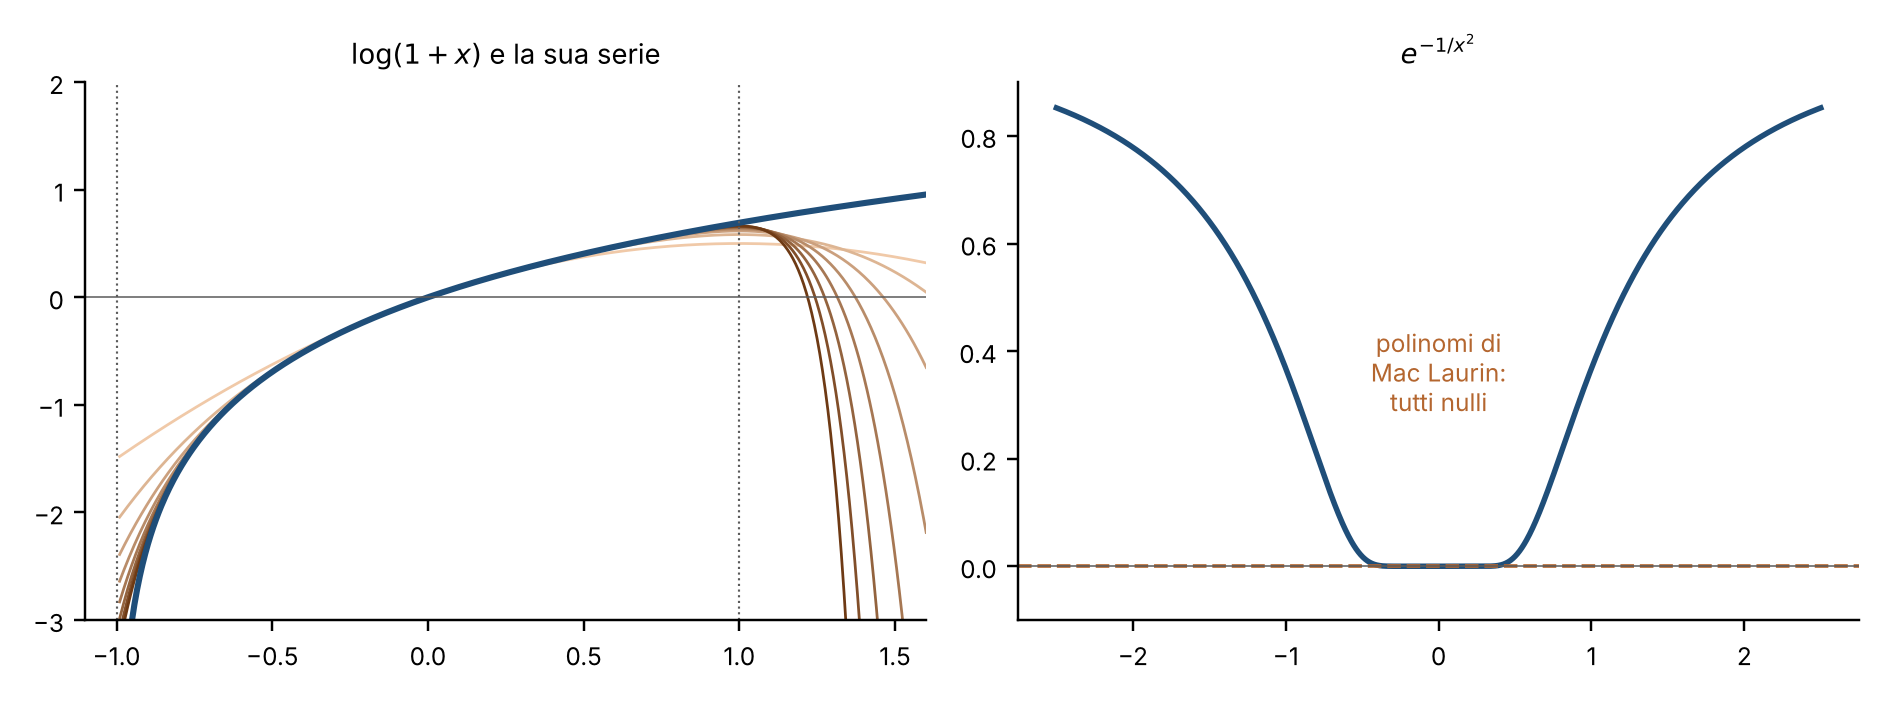
\includegraphics[width=\textwidth]{figure/serie_taylor.png}
\caption{A sinistra: $\log(1+x)$ (blu) e le somme parziali della sua serie di Mac Laurin di
grado $2,4,\dots,16$ (rame): in $(-1,1]$ esse convergono alla funzione, per $x>1$ si
allontanano. A destra: la funzione di Cauchy $e^{-1/x^{2}}$, così piatta nell'origine che tutti
i suoi polinomi di Mac Laurin sono nulli (\texttt{python/fig\_serie\_taylor.py}).}
\label{fig:serie-taylor}
\end{figure}

\subsection{La formula di Eulero}

Nel \cref{cap:complementi} abbiamo introdotto la notazione $e^{i\vartheta}=\cos\vartheta+i\sen\vartheta$
\eqref{eq:eulero}, promettendo di mostrare che si tratta in realtà di un teorema. Le serie
permettono di mantenere la promessa. Diciamo che una successione di numeri complessi
$z_{n}=x_{n}+iy_{n}$ converge a $z=x+iy$ se $x_{n}\to x$ e $y_{n}\to y$, e che una serie di numeri
complessi converge se convergono le sue somme parziali. Poiché la serie esponenziale
\eqref{eq:serie-esponenziale} converge per ogni $x$ reale, è naturale \emph{definire}
l'esponenziale di un numero complesso $z$ come
\begin{equation}\label{eq:esponenziale-complesso}
  e^{z}=\sum_{k=0}^{\infty}\frac{z^{k}}{k!} ,
\end{equation}
definizione che per $z$ reale coincide con l'esponenziale già nota. La serie converge per
ogni $z\in\mathbb C$. Infatti la parte reale e la parte immaginaria di un numero complesso non
superano in valore assoluto il suo modulo, e $\abs{z^{k}}=\abs z^{k}$ (per la
\eqref{eq:prodotto-trigonometrico}); quindi
$\bigl|\operatorname{Re}\frac{z^{k}}{k!}\bigr|\le\frac{\abs z^{k}}{k!}$ e $\bigl|\operatorname{Im}\frac{z^{k}}{k!}\bigr|\le\frac{\abs z^{k}}{k!}$. La serie
$\sum\frac{\abs z^{k}}{k!}$ converge, e per il confronto e il \cref{teo:convergenza-assoluta}
convergono le serie delle parti reali e delle parti immaginarie.

\begin{teorema}[Formula di Eulero]\label{teo:formula-eulero}\index{formula di Eulero}
Per ogni $\vartheta\in\R$ la serie $\sum_{k=0}^{\infty}\frac{(i\vartheta)^{k}}{k!}$ converge, e
\begin{equation}\label{eq:formula-eulero}
  e^{i\vartheta}=\sum_{k=0}^{\infty}\frac{(i\vartheta)^{k}}{k!}=\cos\vartheta+i\sen\vartheta .
\end{equation}
\end{teorema}

\begin{schema}
\Ipotesi{$\vartheta\in\R$; \ $e^{z}$ definito dalla \eqref{eq:esponenziale-complesso}; \ le serie
\eqref{eq:serie-seno} e \eqref{eq:serie-coseno}.}
\Tesi{$\sum_{k=0}^{\infty}\frac{(i\vartheta)^{k}}{k!}=\cos\vartheta+i\sen\vartheta$.}
\end{schema}

\begin{strategia}
Le potenze di $i$ valgono ciclicamente $1,i,-1,-i$: nella serie esponenziale calcolata in
$i\vartheta$, i termini di indice pari sono reali e riproducono, con i loro segni alterni, la serie
del coseno; quelli di indice dispari sono immaginari e riproducono la serie del seno.
Basta allora separare parte reale e parte immaginaria delle somme parziali e
riconoscere in esse le somme parziali delle due serie note.
\end{strategia}

\begin{dimostrazione}
Le potenze di $i$ si ripetono con periodo $4$: $i^{2m}=(-1)^{m}$ e $i^{2m+1}=(-1)^{m}i$. Quindi i
termini di indice pari della serie sono reali, $\frac{(i\vartheta)^{2m}}{(2m)!}=(-1)^{m}\frac{\vartheta^{2m}}{(2m)!}$, e
quelli di indice dispari sono immaginari puri,
$\frac{(i\vartheta)^{2m+1}}{(2m+1)!}=i\,(-1)^{m}\frac{\vartheta^{2m+1}}{(2m+1)!}$. La parte reale della somma parziale
$S_{n}=\sum_{k=0}^{n}\frac{(i\vartheta)^{k}}{k!}$ è allora la somma dei termini della serie del coseno
\eqref{eq:serie-coseno} con $2m\le n$, e la parte immaginaria è la somma dei termini della
serie del seno \eqref{eq:serie-seno} con $2m+1\le n$. Dette $C_{m}$ e $D_{m}$ le somme parziali
$m$-esime delle serie del coseno e del seno (con $m+1$ termini), si ha dunque
$\operatorname{Re}S_{2m}=\operatorname{Re}S_{2m+1}=C_{m}$ e $\operatorname{Im}S_{2m+1}=\operatorname{Im}S_{2m+2}=D_{m}$:
le estratte di indici pari e dispari di $\operatorname{Re}S_{n}$ tendono entrambe a $\cos\vartheta$, quelle di
$\operatorname{Im}S_{n}$ a $\sen\vartheta$, e per il \cref{lem:pari-dispari} si ha
$S_{n}\to\cos\vartheta+i\sen\vartheta$.
\end{dimostrazione}

Con $\vartheta=\pi$ si ottiene la celebre identità $e^{i\pi}+1=0$, che lega i cinque numeri più
importanti della matematica. Ora che $e^{i\vartheta}$ è definito dalla serie, la
\eqref{eq:prodotto-esponenziale} del \cref{cap:complementi},
$e^{i\vartheta}e^{i\vartheta'}=e^{i(\vartheta+\vartheta')}$, è un teorema: segue dalla formula di Eulero e dalle
formule di addizione, attraverso la \eqref{eq:prodotto-trigonometrico}. Per dimostrare
invece che $e^{z+w}=e^{z}e^{w}$ per $z$ e $w$ complessi qualsiasi occorre una regola per
moltiplicare due serie (il \emph{prodotto di Cauchy}), che si studia nei corsi
successivi.

\begin{python}[Serie di Taylor al lavoro]
import math

def exp_serie(x, N=100):
    """Somma dei primi N termini della serie esponenziale."""
    t, s = 1.0, 1.0
    for k in range(1, N):
        t *= x / k
        s += t
    return s

for x in (1.0, 5.0, -10.0, -20.0):
    print(f"x = {x:6.1f}: serie {exp_serie(x):.10e}   "
          f"exp {math.exp(x):.10e}")
print(f"e^-20 come 1/serie(20): {1 / exp_serie(20.0):.10e}")

lento = sum((-1)**(k - 1) / k for k in range(1, 11))
veloce = 2 * sum((1/3)**(2*k + 1) / (2*k + 1) for k in range(10))
print(f"log 2: lenta {lento:.6f}, veloce {veloce:.12f}, "
      f"esatto {math.log(2):.12f}")
print("e^(i pi) =", sum((1j * math.pi)**k / math.factorial(k)
                        for k in range(40)))
\end{python}
\begin{risultato}
x =    1.0: serie 2.7182818285e+00   exp 2.7182818285e+00
x =    5.0: serie 1.4841315910e+02   exp 1.4841315910e+02
x =  -10.0: serie 4.5399929670e-05   exp 4.5399929762e-05
x =  -20.0: serie 6.1475618289e-09   exp 2.0611536224e-09
e^-20 come 1/serie(20): 2.0611536224e-09
log 2: lenta 0.645635, veloce 0.693147180550, esatto 0.693147180560
e^(i pi) = (-1.0000000000000002+3.4586691443274427e-16j)
\end{risultato}

Il programma mette in luce un fatto importante per il calcolo numerico: per $x$ negativo
e grande in valore assoluto la serie esponenziale ha termini grandi di segno alterno, che
si cancellano quasi completamente, e la somma calcolata in virgola mobile perde tutte le
cifre significative. Il rimedio è calcolare $e^{x}=\frac1{e^{\abs x}}$ con la serie a termini
positivi: matematicamente le due strade sono equivalenti, numericamente no.

\needspace{10\baselineskip}
\begin{notastorica}[Le serie di potenze]
Isaac Newton scoprì nel 1665 la serie binomiale $(1+x)^{b}=\sum\binom bk x^{k}$ per esponenti $b$
qualsiasi, e ne fece lo strumento principale del suo calcolo; James Gregory (1671), Brook Taylor (1715) e
Colin Mac Laurin (1742) diedero il metodo generale per ottenere la serie di una funzione dalle
sue derivate. Eulero, nell'\emph{Introductio in analysin infinitorum} (1748), fondò sulle
serie di potenze la teoria delle funzioni elementari, ricavando tra l'altro la formula
che porta il suo nome. Per tutto il Settecento si ritenne, con Lagrange, che ogni funzione
«ragionevole» fosse uguale alla propria serie di Taylor; il controesempio di Cauchy, del
1823, mostrò che la derivabilità infinita non basta. Le funzioni sviluppabili in serie di
Taylor in un intorno di ogni punto si chiamano oggi \emph{analitiche}, e il loro studio,
che si svolge in modo naturale nel campo complesso, è uno dei capitoli più belli
dell'analisi.
\end{notastorica}

%% ----------------------------------------------------------------------------
%%  §11.10  Esercizi di riepilogo
%% ----------------------------------------------------------------------------
\section{Esercizi di riepilogo}
\label{sec:esercizi-cap11}

Come nei capitoli precedenti, ogni soluzione è accompagnata da una nota sulla
\emph{scelta logica} che la guida.

\needspace{8\baselineskip}
\subsection*{Somme di serie}

\begin{esercizio}
Calcolare $\displaystyle\sum_{k=1}^{\infty}\frac1{k(k+2)}$.
\begin{soluzione}
Decomponendo in fratti semplici, $\frac1{k(k+2)}=\frac12\bigl(\frac1k-\frac1{k+2}\bigr)$. Posto
$b_{k}=\frac1k+\frac1{k+1}$, si ha $b_{k}-b_{k+1}=\frac1k-\frac1{k+2}$, e per la \cref{prop:serie-telescopica}
$\sum_{k=1}^{\infty}\bigl(\frac1k-\frac1{k+2}\bigr)=b_{1}-\lim b_{n}=1+\frac12=\frac32$. Per la linearità la somma
cercata è $\frac34$. \emph{Scelta logica:} quando il termine generale è una funzione razionale,
la decomposizione in fratti semplici può rivelare una struttura telescopica; qui i
termini si elidono «a distanza due», e il trucco è raggruppare due addendi consecutivi
in $b_{k}$.
\end{soluzione}
\end{esercizio}

\begin{esercizio}
Studiare la serie $\sum_{k=1}^{\infty}\log\bigl(1+\frac1k\bigr)$.
\begin{soluzione}
Si ha $\log\bigl(1+\frac1k\bigr)=\log(k+1)-\log k=b_{k}-b_{k+1}$ con $b_{k}=-\log k$: per la
\cref{prop:serie-telescopica}, $s_{n}=\log(n+1)$, e poiché $b_{n}\to-\infty$ la serie diverge a
$+\infty$. In alternativa: $\log\bigl(1+\frac1n\bigr)\sim\frac1n$, e il confronto asintotico
(\cref{cor:confronto-asintotico}) con la serie armonica dà la divergenza.
\emph{Scelta logica:} il termine generale tende a zero, ma la condizione necessaria non
basta; due strade indipendenti (somma esplicita, parte principale) conducono alla stessa
conclusione.
\end{soluzione}
\end{esercizio}

\begin{esercizio}
Calcolare $\displaystyle\sum_{k=1}^{\infty}\frac{2^{k}+3^{k}}{6^{k}}$.
\begin{soluzione}
Il termine generale è $\bigl(\frac13\bigr)^{k}+\bigl(\frac12\bigr)^{k}$. Per la \eqref{eq:geometrica-generale}
con $m=1$, $\sum_{k\ge1}\bigl(\frac13\bigr)^{k}=\frac{1/3}{1-1/3}=\frac12$ e $\sum_{k\ge1}\bigl(\frac12\bigr)^{k}=1$; per la linearità
la somma è $\frac32$. \emph{Scelta logica:} si spezza il termine generale in somma di termini
geometrici; la linearità è lecita perché entrambe le serie convergono.
\end{soluzione}
\end{esercizio}

\begin{esercizio}
Per quali $x>0$ converge la serie $\sum_{k=0}^{\infty}(\log x)^{k}$? Calcolarne la somma.
\begin{soluzione}
È una serie geometrica di ragione $\log x$: converge se e solo se $\abs{\log x}<1$, cioè
$\frac1e<x<e$, e la somma è $\frac1{1-\log x}$. Per $x\ge e$ diverge, per $0<x\le\frac1e$ è indeterminata.
\emph{Scelta logica:} riconoscere una serie geometrica «travestita» è il primo passo di
fronte a una serie i cui termini sono potenze di un'unica espressione.
\end{soluzione}
\end{esercizio}

\begin{esercizio}
Calcolare $\displaystyle\sum_{k=0}^{\infty}\frac k{k!}$ e $\displaystyle\sum_{k=0}^{\infty}\frac{k^{2}}{k!}$.
\begin{soluzione}
Per $k\ge1$, $\frac k{k!}=\frac1{(k-1)!}$; il termine con $k=0$ è nullo. Quindi
$\sum_{k=0}^{\infty}\frac k{k!}=\sum_{j=0}^{\infty}\frac1{j!}=e$ per la \eqref{eq:e-serie} (con $j=k-1$). Analogamente
$\frac{k^{2}}{k!}=\frac k{(k-1)!}=\frac{(k-1)+1}{(k-1)!}$, e per $k\ge2$ si ha $\frac{k-1}{(k-1)!}=\frac1{(k-2)!}$; dunque
$\sum_{k=0}^{\infty}\frac{k^{2}}{k!}=\sum_{j=0}^{\infty}\frac1{j!}+\sum_{j=0}^{\infty}\frac1{j!}=2e$. \emph{Scelta logica:} semplificando il
fattoriale e cambiando indice ci si riconduce alla serie esponenziale; la linearità è
lecita perché tutte le serie coinvolte convergono.
\end{soluzione}
\end{esercizio}

\needspace{8\baselineskip}
\subsection*{Criteri di convergenza}

\begin{esercizio}\label{es:carattere}
Studiare il carattere delle serie
(a) $\sum\frac{k+1}{k^{3}+2}$; \ (b) $\sum\frac1{\sqrt{k(k+1)}}$; \ (c) $\sum\frac{k^{2}}{3^{k}}$; \
(d) $\sum\frac{k!}{(2k)!}$; \ (e) $\sum\bigl(1-\frac1k\bigr)^{k^{2}}$; \ (f) $\sum_{k\ge2}\frac1{\log k}$.
\begin{soluzione}
(a) Converge: $n^{2}\cdot\frac{n+1}{n^{3}+2}\to1$, criterio degli infinitesimi con $p=2$.
(b) Diverge: $n\cdot\frac1{\sqrt{n(n+1)}}\to1$, con $p=1$.
(c) Converge per il criterio del rapporto: $\frac{(n+1)^{2}}{3^{n+1}}\cdot\frac{3^{n}}{n^{2}}\to\frac13$.
(d) Converge per il criterio del rapporto: $\frac{(n+1)!}{(2n+2)!}\cdot\frac{(2n)!}{n!}=\frac{n+1}{(2n+1)(2n+2)}\to0$.
(e) Converge per il criterio della radice: $\sqrt[n]{a_{n}}=\bigl(1-\frac1n\bigr)^{n}\to\frac1e<1$
(\cref{teo:e-generalizzato}).
(f) Diverge per il confronto: $\log k<k$, e quindi $\frac1{\log k}>\frac1k$.
\emph{Scelta logica:} il criterio si sceglie guardando la forma del termine generale:
potenze di $n$ (confronto, infinitesimi), esponenziali e fattoriali (rapporto), potenze
con esponente $n$ (radice).
\end{soluzione}
\end{esercizio}

\needspace{7\baselineskip}
\begin{esercizio}
Per quali $\alpha>0$ converge la serie $\sum_{k=1}^{\infty}\bigl(e^{1/k^{\alpha}}-1\bigr)$?
\begin{soluzione}
I termini sono positivi. Dallo sviluppo $e^{t}-1=t+o(t)$ con $t=\frac1{n^{\alpha}}\to0$ si ha
$e^{1/n^{\alpha}}-1\sim\frac1{n^{\alpha}}$, e per il confronto asintotico la serie ha lo stesso carattere
dell'armonica generalizzata con $p=\alpha$: converge se e solo se $\alpha>1$. \emph{Scelta logica:}
la parte principale del termine generale riduce ogni serie di questo tipo a una serie
armonica generalizzata.
\end{soluzione}
\end{esercizio}

\begin{esercizio}
Quanti termini della serie $\sum\frac1{k^{3}}$ occorre sommare per avere la somma con un
errore inferiore a $10^{-4}$?
\begin{soluzione}
Per la \eqref{eq:resto-integrale-serie} con $f(x)=\frac1{x^{3}}$, il resto verifica
$R_{n}\le\int_{n}^{+\infty}\frac{dx}{x^{3}}=\frac1{2n^{2}}$. Basta $\frac1{2n^{2}}<10^{-4}$, cioè $n^{2}>5000$, $n\ge71$. La
stima dal basso $R_{n}\ge\frac1{2(n+1)^{2}}$ mostra che non si può fare molto meglio: per $n=60$
l'errore è certamente maggiore di $10^{-4}$. \emph{Scelta logica:} per le serie a termini
positivi e decrescenti il criterio dell'integrale fornisce non soltanto il carattere, ma
anche una stima del resto dall'alto e dal basso.
\end{soluzione}
\end{esercizio}

\needspace{8\baselineskip}
\subsection*{Serie a segni alterni e convergenza assoluta}

\begin{esercizio}
Dimostrare che $\sum_{k=1}^{\infty}(-1)^{k}\frac k{k^{2}+1}$ converge, ma non assolutamente.
\begin{soluzione}
La funzione $g(x)=\frac x{x^{2}+1}$ ha derivata $g'(x)=\frac{1-x^{2}}{(x^{2}+1)^{2}}\le0$ per $x\ge1$: la
successione $a_{n}=g(n)$ è decrescente, positiva e infinitesima, e la serie converge per il
criterio di Leibniz. La serie dei valori assoluti diverge, perché $\frac n{n^{2}+1}\sim\frac1n$.
\emph{Scelta logica:} la monotonia di una successione definita da una funzione si
verifica comodamente con il segno della derivata.
\end{soluzione}
\end{esercizio}

\begin{esercizio}
Calcolare $\sum_{k=1}^{\infty}\frac{(-1)^{k-1}}{k^{3}}$ con un errore inferiore a $10^{-3}$.
\begin{soluzione}
La serie verifica le ipotesi del criterio di Leibniz, e per la \eqref{eq:stima-leibniz}
basta $\frac1{(n+1)^{3}}\le10^{-3}$, cioè $n+1\ge10$. La somma dei primi $9$ termini è
$s_{9}\approx0{,}90212$, e la somma vera è compresa tra $s_{10}=s_{9}-10^{-3}$ e $s_{9}$; poiché i termini sono
strettamente decrescenti, essa è diversa da entrambi (le estratte pari e dispari sono
strettamente monotòne), e l'errore è strettamente minore di $10^{-3}$. Il valore è
$0{,}901543\ldots$ \emph{Scelta logica:} la serie converge anche assolutamente, ma per la
stima dell'errore il criterio di Leibniz è molto più preciso di quello dell'integrale
applicato alla serie dei valori assoluti.
\end{soluzione}
\end{esercizio}

\begin{esercizio}\label{es:serie-xk-su-k}
Determinare gli $x\in\R$ per cui converge la serie $\sum_{k=1}^{\infty}\frac{x^{k}}k$, e calcolarne la
somma.
\begin{soluzione}
Il rapporto dei valori assoluti è $\frac{\abs x\,n}{n+1}\to\abs x$: per il \cref{cor:rapporto-assoluto}
la serie converge assolutamente se $\abs x<1$ e non converge se $\abs x>1$. Per $x=1$ è la
serie armonica, divergente; per $x=-1$ è l'opposto della serie armonica alternata,
convergente. Dunque la serie converge se e solo se $-1\le x<1$, e, per la \eqref{eq:serie-log}
con $-x$ al posto di $x$, la somma è $-\log(1-x)$. \emph{Scelta logica:} il criterio del
rapporto decide all'interno e all'esterno dell'intervallo $(-1,1)$, ma non agli estremi,
dove $\ell=1$: lì servono considerazioni specifiche.
\end{soluzione}
\end{esercizio}

\needspace{8\baselineskip}
\subsection*{Applicazioni}

\begin{esercizio}[Resistenza indotta di un'ala non ellittica]
Per un'ala simmetrica i coefficienti di Glauert valgono $\frac{A_{3}}{A_{1}}=0{,}05$, $\frac{A_{5}}{A_{1}}=0{,}01$,
e i successivi sono trascurabili. Stimare l'aumento percentuale della resistenza indotta
rispetto all'ala ellittica con la stessa portanza e lo stesso allungamento.
\begin{soluzione}
Per la \eqref{eq:resistenza-indotta}, $\delta\approx3\cdot0{,}05^{2}+5\cdot0{,}01^{2}=0{,}0075+0{,}0005=0{,}008$: la
resistenza indotta è maggiore di circa lo $0{,}8\%$. Poiché la serie è a termini non
negativi, trascurare i termini successivi porta a una stima \emph{per difetto} di $\delta$.
\emph{Scelta logica:} in una serie a termini non negativi ogni somma parziale è un
minorante della somma; il segno dell'errore di troncamento è quindi noto.
\end{soluzione}
\end{esercizio}

\begin{esercizio}[Un rimbalzo smorzato]
Un corpo lasciato cadere da un'altezza $h_{0}$ rimbalza ogni volta fino a un'altezza pari a
una frazione $r<1$ della precedente. Calcolare lo spazio totale percorso e la durata
totale del moto, trascurando la resistenza dell'aria e la durata degli urti.
\begin{soluzione}
Lo spazio è $h_{0}+2rh_{0}+2r^{2}h_{0}+\dots=h_{0}+2h_{0}\frac r{1-r}=h_{0}\frac{1+r}{1-r}$. Il tempo di caduta da
un'altezza $h$ è $\sqrt{2h/g}$, e quindi una salita e una discesa dall'altezza $r^{k}h_{0}$ durano
$2\sqrt{2h_{0}/g}\,(\sqrt r)^{k}$. La durata totale è
$t_{0}+2t_{0}\sum_{k\ge1}(\sqrt r)^{k}=t_{0}\frac{1+\sqrt r}{1-\sqrt r}$, con $t_{0}=\sqrt{2h_{0}/g}$: infiniti rimbalzi in
un tempo finito (il numero $\sqrt r$ è il coefficiente di restituzione dell'urto; gli
infiniti rimbalzi sono naturalmente un'idealizzazione del modello). Con $h_{0}=1$~m e
$r=0{,}64$ lo spazio è $4{,}56$~m e la durata
$9t_{0}\approx4{,}06$~s. \emph{Scelta logica:} ogni grandezza che si riduce a ogni passo di un
fattore costante dà luogo a una serie geometrica; spazio e tempo sono due serie
geometriche di ragioni diverse, $r$ e $\sqrt r$.
\end{soluzione}
\end{esercizio}

\begin{python}[Verifica degli esercizi]
import math
import sympy as sp

k = sp.symbols('k', integer=True, positive=True)
print(sp.summation(1 / (k * (k + 2)), (k, 1, sp.oo)))
print(sp.summation((2**k + 3**k) / 6**k, (k, 1, sp.oo)))
print(sp.summation(k / sp.factorial(k), (k, 1, sp.oo)),
      sp.summation(k**2 / sp.factorial(k), (k, 1, sp.oo)))
s3 = sp.summation((-1)**(k - 1) / k**3, (k, 1, sp.oo))
print(s3, "=", sp.N(s3, 8))
s9 = sum((-1)**(j - 1) / j**3 for j in range(1, 10))
print(f"s_9 = {s9:.6f}")
n = next(n for n in range(1, 1000) if 1 / (2 * n**2) < 1e-4)
print("termini per 1/k^3 con errore < 1e-4:", n)
r, t0 = 0.64, math.sqrt(2 / 9.81)
print(f"rimbalzi: spazio {(1+r)/(1-r):.2f} m, durata "
      f"{t0 * (1 + math.sqrt(r)) / (1 - math.sqrt(r)):.2f} s")
\end{python}
\begin{risultato}
3/4
3/2
E 2*E
dirichlet_eta(3) = 0.90154268
s_9 = 0.902116
termini per 1/k^3 con errore < 1e-4: 71
rimbalzi: spazio 4.56 m, durata 4.06 s
\end{risultato}

%% ----------------------------------------------------------------------------
%%  §11.11  Punti fondamentali del capitolo
%% ----------------------------------------------------------------------------
\section{Punti fondamentali del capitolo}
\label{sec:sintesi-cap11}

Una serie è la successione delle sue somme parziali, e tutta la teoria poggia sui limiti
di successioni. Poiché la somma si sa calcolare solo in pochi casi, il cuore del capitolo
sono i criteri che ne decidono il carattere confrontando il termine generale con due
modelli, la serie geometrica e l'armonica generalizzata. La convergenza assoluta estende
i criteri alle serie di segno qualsiasi, e le serie di Taylor rappresentano le funzioni
elementari come «polinomi di grado infinito».

\begin{puntichiave}
\item \textbf{Serie e carattere.} La serie $\sum a_{k}$ è la successione delle somme parziali
$s_{n}=a_{1}+\dots+a_{n}$: è convergente, divergente o indeterminata secondo che $s_{n}$ abbia
limite finito, limite infinito o nessun limite (\cref{def:serie}). Modificare un numero
finito di termini non cambia il carattere, e per una serie convergente il resto
$R_{n}=s-s_{n}$ tende a zero (\cref{teo:resto-serie}).
\item \textbf{Condizione necessaria.} Se $\sum a_{k}$ converge, allora $a_{n}\to0$
(\cref{teo:condizione-necessaria}). La condizione non è sufficiente, come mostrano la serie
armonica e la serie telescopica $\sum\bigl(\sqrt{k+1}-\sqrt k\bigr)$: serve soltanto a escludere la
convergenza, e usarla «in positivo» è l'errore più frequente.
\item \textbf{Serie telescopiche e criterio di Cauchy.} Se $a_{k}=b_{k}-b_{k+1}$, allora
$s_{n}=b_{1}-b_{n+1}$ e la serie ha il carattere della successione $b_{n}$
(\cref{prop:serie-telescopica}). Senza conoscerne la somma, la serie converge se e solo se
per ogni $\epsilon>0$ esiste $\nu$ tale che $\abs{a_{n+1}+\dots+a_{n+p}}<\epsilon$ per ogni $n>\nu$ e
ogni $p\in\N$ (\cref{teo:cauchy-serie}).
\item \textbf{Termini non negativi.} Se $a_{n}\ge0$ la serie non è mai indeterminata:
converge se e solo se le somme parziali sono limitate, e allora $\sum a_{k}=\sup_{n}s_{n}$
(\cref{teo:serie-positive}). Ogni somma parziale è quindi un'approssimazione per difetto
della somma.
\item \textbf{Le serie modello.} La serie geometrica $\sum_{k\ge0}x^{k}$ converge se e solo se
$\abs x<1$, con somma $\frac1{1-x}$; diverge a $+\infty$ per $x\ge1$ ed è indeterminata per
$x\le-1$ (\cref{teo:serie-geometrica}). L'armonica generalizzata $\sum\frac1{k^{p}}$ converge
se e solo se $p>1$ (\cref{teo:armonica-generalizzata}); per $p=1$ le somme parziali
divergono come $\log n$, e $H_{n}-\log n\to\gamma$ (\cref{teo:armonica,prop:eulero-mascheroni}).
\item \textbf{Criterio dell'integrale.} Se $f$ è continua, non negativa e decrescente in
$[1,+\infty)$, la serie $\sum f(k)$ e l'integrale improprio $\int_{1}^{+\infty}f(x)\,dx$
convergono o divergono insieme, e il resto verifica
$\int_{n+1}^{+\infty}f\le R_{n}\le\int_{n}^{+\infty}f$ (\cref{teo:criterio-integrale}).
\item \textbf{Confronto.} Se $0\le a_{n}\le b_{n}$ da un certo indice in poi, la convergenza
di $\sum b_{k}$ implica quella di $\sum a_{k}$, e la divergenza di $\sum a_{k}$ implica quella di
$\sum b_{k}$ (\cref{teo:confronto-serie}). Se $a_{n}\ge0$, $b_{n}>0$ e
$\frac{a_{n}}{b_{n}}\to L\in(0,+\infty)$, le due serie hanno lo stesso carattere
(\cref{cor:confronto-asintotico}).
\item \textbf{Infinitesimi e parte principale.} Se $a_{n}\ge0$ e $n^{p}a_{n}\to\ell$, la serie
converge per $\ell<+\infty$ e $p>1$, diverge per $\ell>0$ e $p\le1$
(\cref{teo:criterio-infinitesimi}). In pratica si determina la parte principale del
termine generale con gli sviluppi di Taylor del \cref{cap:taylor}.
\item \textbf{Rapporto e radice.} Se $a_{n}>0$ e $\frac{a_{n+1}}{a_{n}}\to\ell$, oppure $a_{n}\ge0$ e
$\sqrt[n]{a_{n}}\to\ell$, la serie converge per $\ell<1$ e diverge per $\ell>1$
(\cref{teo:criterio-rapporto-serie,teo:criterio-radice}): sono i criteri adatti a
fattoriali e potenze di esponente $n$. Per $\ell=1$ non decidono, ed è il caso di tutte le
serie $\sum\frac1{k^{p}}$.
\item \textbf{Criterio di Leibniz.} Se $a_{n}\ge0$ è decrescente e infinitesima, la serie
$\sum(-1)^{k-1}a_{k}$ converge e $\abs{s-s_{n}}\le a_{n+1}$: l'errore è maggiorato dal primo
termine trascurato e ne ha il segno (\cref{teo:leibniz}). L'ipotesi di monotonia non si
può omettere.
\item \textbf{Convergenza assoluta.} Se $\sum\abs{a_{k}}$ converge, converge anche $\sum a_{k}$, e
$\abs{\sum a_{k}}\le\sum\abs{a_{k}}$ (\cref{teo:convergenza-assoluta}); il viceversa è falso, come
mostra la serie armonica alternata. I criteri del rapporto e della radice applicati a
$\abs{a_{n}}$ danno la convergenza assoluta per $\ell<1$ e la non convergenza per $\ell>1$
(\cref{cor:rapporto-assoluto}).
\item \textbf{Riordinamenti.} Ogni riordinamento di una serie assolutamente convergente
converge assolutamente alla stessa somma (\cref{teo:dirichlet-riordinamento}). Una serie
semplicemente convergente si può invece riordinare in modo da ottenere qualunque somma
in $\overline\R$ (\cref{teo:riemann-riordinamento}): riordinata con due termini positivi e
uno negativo, la serie armonica alternata ha somma $\frac32\log2$ (\cref{es:riordinamento}).
\item \textbf{Serie di Taylor.} La serie di Taylor di $f$ converge a $f(x)$ se e solo se il
resto $R_{n}(x)$ tende a zero; basta che tutte le derivate siano limitate da una stessa
costante in $[x_{0}-\delta,x_{0}+\delta]$ (\cref{teo:sviluppabilita}). Così $e^{x}$, $\sen x$ e $\cos x$
sono somme delle loro serie per ogni $x\in\R$, $\log(1+x)$ per $-1<x\le1$ e
$\operatorname{arctg}x$ per $\abs x\le1$ (\cref{es:serie-elementari,prop:serie-log-arctg}), mentre
$e^{-1/x^{2}}$ non è sviluppabile in $0$ (\cref{prop:cauchy-controesempio}). Definito $e^{z}$
con la serie, $e^{i\vartheta}=\cos\vartheta+i\sen\vartheta$ diventa un teorema (\cref{teo:formula-eulero}).
\item \textbf{Resistenza indotta.} Nella teoria di Prandtl e Glauert
$C_{D,i}=\frac{C_{L}^{2}}{\pi\,AR}(1+\delta)$, dove $\delta=\sum_{n\ge2}n\bigl(\frac{A_{n}}{A_{1}}\bigr)^{2}$ è la
somma di una serie a termini non negativi \eqref{eq:resistenza-indotta}: a parità di
$C_{L}$ e di $AR$ la resistenza indotta è minima, cioè $\delta=0$, se e solo se la
distribuzione di circolazione è ellittica.
\end{puntichiave}

\section*{Uno sguardo oltre}
\addcontentsline{toc}{section}{Uno sguardo oltre}

Con le serie si chiude questo primo volume. Il lettore che ci ha seguiti fin qui ha
percorso la strada che va dagli assiomi dei numeri reali al calcolo differenziale e
integrale, e ha visto come tutto discenda, attraverso una catena di teoremi di
esistenza, dall'assioma di completezza (\cref{fig:schema-teoremi}). Molte domande, però,
sono rimaste aperte, e indicano la strada dei corsi successivi.

\begin{itemize}
  \item Abbiamo sommato serie di \emph{numeri}. Le serie di Taylor sono invece serie di
  \emph{funzioni}, e per derivarle o integrarle termine a termine (ad esempio per calcolare
  $\int_{0}^{1}e^{-x^{2}}dx$ integrando la serie esponenziale) occorre un tipo di convergenza più
  forte, la \emph{convergenza uniforme}.
  \item La serie di Taylor dell'arcotangente non converge per $\abs x>1$, pur essendo la
  funzione regolarissima su tutto $\R$ (\cref{prop:serie-log-arctg,fig:taylor-arctg}). La
  spiegazione viene dalle \emph{serie di potenze} nel campo complesso, dove la sua derivata
  $\frac1{1+z^{2}}$ ha due singolarità, $z=\pm i$, a distanza $1$ dall'origine: il \emph{raggio di
  convergenza} della serie (\cref{oss:raggio-convergenza}) è proprio questa distanza.
  \item La serie di Glauert \eqref{eq:glauert} è una serie di seni: un esempio di
  \emph{serie di Fourier}, lo strumento con cui si studiano le vibrazioni delle strutture,
  il flutter, l'acustica e l'elaborazione dei segnali.
  \item Le grandezze dell'ingegneria dipendono quasi sempre da più variabili: il
  \cref{cap:piu-variabili} ne ha dato un primo assaggio, ma il calcolo integrale in più
  variabili resta da costruire. Le leggi della fisica, poi, si esprimono con
  \emph{equazioni differenziali}: la linea elastica \eqref{eq:linea-elastica}
  ne è un primo esempio, e la dinamica del volo, la meccanica dei fluidi e la meccanica
  delle strutture ne sono piene.
\end{itemize}

Sono gli argomenti dell'Analisi Matematica Due. Ma il metodo resta lo stesso che abbiamo
cercato di praticare in queste pagine: dire con esattezza che cosa si suppone e che cosa
si vuole dimostrare, avere un piano prima di cominciare, e verificare, anche con un
calcolatore, che ciò che si è dimostrato descriva davvero il mondo.



%% ============================ APPENDICI ====================================
\appendix
% \input{capitoli/appA-...}

%% ============================ PAGINE FINALI ================================
\backmatter
% due righe in più nell'ultima pagina dell'indice, perché la voce finale non resti sola
\addtocontents{toc}{\protect\enlargethispage{3\baselineskip}}
%% ============================================================================
%%  Bibliografia
%% ============================================================================
\begin{thebibliography}{9}
\addcontentsline{toc}{chapter}{Bibliografia}

\bibitem{marcellini-sbordone}
P.~Marcellini, C.~Sbordone, \emph{Elementi di Analisi Matematica uno}, Liguori Editore,
Napoli, 2002.

\bibitem{marcellini-sbordone-es}
P.~Marcellini, C.~Sbordone, \emph{Esercitazioni di Matematica}, vol.~1, parti prima e
seconda, Liguori Editore, Napoli.

\bibitem{giusti}
E.~Giusti, \emph{Analisi Matematica 1}, terza edizione, Bollati Boringhieri, Torino,
2003.

\bibitem{giusti2}
E.~Giusti, \emph{Analisi Matematica 2}, seconda edizione, Bollati Boringhieri, Torino,
1989.

\bibitem{tao1}
T.~Tao, \emph{Analysis I}, third edition, Texts and Readings in Mathematics 37,
Hindustan Book Agency / Springer, 2016.

\bibitem{tao2}
T.~Tao, \emph{Analysis II}, Texts and Readings in Mathematics 38, Hindustan Book Agency,
2006.

\bibitem{paolini}
E.~Paolini, \emph{Analisi Uno}, dispense rilasciate con licenza CC~BY-SA,
\url{https://github.com/paolini/AnalisiUno}.

\bibitem{dedekind}
R.~Dedekind, \emph{Stetigkeit und irrationale Zahlen}, Vieweg, Braunschweig, 1872
(trad.\ it.\ \emph{Continuità e numeri irrazionali}, in \emph{Scritti sui fondamenti
della matematica}, Bibliopolis, Napoli, 1982).

\bibitem{florilegium}
K.~Raymond, \emph{florilegium} --- procedurally generated floral page margins for
LuaLaTeX, \url{https://github.com/kevinraymond/florilegium}, licenza MIT.
\end{thebibliography}

\cleardoublepage
\printindex

\end{document}
